% book-vol2.tex — LeetCUDA 技术书下册（第四部分后半 + 第五～九部分，第 24--45 章 + 附录 A--E）
% 构建：cd book/ && ./build.sh（全量，默认）或 ./build.sh --only v2
% 全一册版仍是 book.tex；本文件与 book-vol1.tex 是它的两段切分，章号/图号/表号/公式号连续。
\documentclass[9pt,openany]{ctexbook}
% preamble.tex — LeetCUDA 技术书导言
% 抽取自 tex/notes-v2.tex（8 色调色板/字体/lstset），ctexart → ctexbook
% RFC-0.2 / RFC-0.4 关键字表已审计（2026-09-11，grep 全源码验证）

\usepackage[paperwidth=210mm,paperheight=297mm,left=1.35cm,right=1.35cm,top=1.4cm,bottom=1.6cm]{geometry}
\raggedbottom % 页面底部不拉伸胶水（消除列表项间/公式旁被 \flushbottom 拉大的空白）
\usepackage{listings,xcolor,fancyhdr}
\usepackage{graphicx}
\usepackage{needspace}
\usepackage{amsmath,amssymb}
\usepackage{amsthm}
\usepackage{booktabs}
\usepackage{longtable}
\usepackage{enumitem}
\usepackage{tikz}
\usetikzlibrary{matrix,positioning,patterns,arrows.meta,shapes,calc,fit}
\usepackage{subcaption}
\usepackage{array}
\usepackage{adjustbox}

% 长行内代码（\texttt 标识符/路径）混排中文时的断行弹性，压制 Overfull \hbox
\emergencystretch=2em

\pagestyle{fancy}
\fancyhf{}
\fancyhead[LE]{\scriptsize\leavevmode\leftmark}
\fancyhead[RO]{\scriptsize\leavevmode\rightmark}
\fancyfoot[C]{\scriptsize \thepage}
\renewcommand{\headrulewidth}{0.4pt}
\renewcommand{\footrulewidth}{0pt}

% --- 8 色调色板（VSC 风格，同 notes-v2.tex） ---
\definecolor{vscBackground}{RGB}{248,248,248}
\definecolor{vscText}{RGB}{31,35,40}
\definecolor{vscLineNumber}{RGB}{142,142,142}
\definecolor{vscKeyword}{RGB}{0,90,158}

% TikZ 语义色板（2026-09-20：全图统一着色，替代纯灰度）
% 用法：填充大面积用 tkFill* 浅色系，边框/文字/箭头用主色系；无语义的中性结构可保留灰度
\definecolor{tkBlue}{RGB}{33,113,181}     % 结构/主数据/流水
\definecolor{tkGreen}{RGB}{53,141,106}    % 修复/after/有效/命中
\definecolor{tkOrange}{RGB}{216,130,28}   % 冲突/before/警示过渡
\definecolor{tkRed}{RGB}{203,54,47}       % 错误/溢出/坏例
\definecolor{tkPurple}{RGB}{122,82,158}   % 次要强调/对照
\definecolor{tkFillBlue}{RGB}{232,241,250}
\definecolor{tkFillGreen}{RGB}{230,243,236}
\definecolor{tkFillOrange}{RGB}{252,240,224}
\definecolor{tkFillRed}{RGB}{251,233,231}
\definecolor{tkFillPurple}{RGB}{240,234,247}

% CuTe/GEMM layout 图 8 色 hue 环（cute_gemm 风格：hue=tile 身份，intensity=tile 内位置）
% 与 colfax/cf-macros.tex 保持一致；用法：fill=colorxN!10..!60
\definecolor{colorx1}{RGB}{255,0,0}      % Red
\definecolor{colorx2}{RGB}{255,191,0}    % Orange-yellow
\definecolor{colorx3}{RGB}{128,255,0}    % Yellow-green
\definecolor{colorx4}{RGB}{0,255,128}    % Green-cyan
\definecolor{colorx5}{RGB}{0,255,255}    % Cyan
\definecolor{colorx6}{RGB}{0,128,255}    % Blue
\definecolor{colorx7}{RGB}{128,0,255}    % Indigo
\definecolor{colorx8}{RGB}{255,0,255}    % Magenta
\definecolor{vscComment}{RGB}{0,128,0}
\definecolor{vscAccent}{RGB}{163,21,21}
\definecolor{vscEmphasis}{RGB}{43,145,175}
\definecolor{vscFrame}{RGB}{210,210,210}

\setmonofont{DejaVu Sans Mono}
\setCJKmonofont{Noto Sans Mono CJK SC}

% --- 定理类环境 ---
\newtheorem{theorem}{定理}[chapter]
\newtheorem{lemma}[theorem]{引理}
\theoremstyle{definition}
\newtheorem{definition}[theorem]{定义}
\theoremstyle{remark}
\newtheorem*{remark}{注记}
% 勘误与考据框注（源码注释核查结果，全量记录在 book/CHECKLOG.md）
\newtheoremstyle{kaowustyle}{6pt}{6pt}{\small}{}{\bfseries}{：}{ }{}
\theoremstyle{kaowustyle}
\newtheorem{kaogu}{实践经验}[chapter]

% --- 伪代码清单（E2 修复）：同框灰底，自动行号，# 注释 ---
\lstdefinestyle{pseudo}{
  language=, numbers=left, numberstyle=\scriptsize\color{vscLineNumber},
  basicstyle=\footnotesize\ttfamily\color{vscText},
  comment=[l]{\#}, commentstyle=\color{vscComment},
  keywordstyle=\bfseries\color{vscKeyword},
  morekeywords={function,for,to,do,end,if,then,else,while,return,in,parallel,foreach},
  backgroundcolor=\color{vscBackground}, frame=single, framerule=0.8pt,
  rulecolor=\color{vscFrame}, framesep=6pt, xleftmargin=4pt, xrightmargin=4pt,
  breaklines=true, columns=fullflexible, keepspaces=true, tabsize=2,
  aboveskip=4pt, belowskip=4pt, showstringspaces=false, upquote=true,
}
% --- 终端/测试输出清单（E6 修复）：无行号灰底框 ---
\lstdefinestyle{console}{
  language=, numbers=none,
  basicstyle=\footnotesize\ttfamily\color{vscText},
  backgroundcolor=\color{vscBackground}, frame=single, framerule=0.8pt,
  rulecolor=\color{vscFrame}, framesep=6pt, xleftmargin=4pt, xrightmargin=4pt,
  breaklines=true, columns=fullflexible, keepspaces=true, tabsize=2,
  aboveskip=4pt, belowskip=4pt, showstringspaces=false, upquote=true,
}

% --- 代码清单：firstnumber=auto（行号与源文件一致） ---
\lstset{
  language=C,
  basicstyle=\footnotesize\ttfamily\color{vscText},
  numbers=left,
  numberstyle=\scriptsize\color{vscLineNumber},
  numbersep=6pt,
  showstringspaces=false,
  breaklines=true,
  breakatwhitespace=false,
  tabsize=2,
  extendedchars=true,
  upquote=true,
  columns=fullflexible,
  keepspaces=true,
  backgroundcolor=\color{vscBackground},
  frame=single,
  framerule=0.8pt,
  rulecolor=\color{vscFrame},
  framesep=6pt,
  xleftmargin=4pt,
  xrightmargin=4pt,
  aboveskip=4pt,
  belowskip=4pt,
  firstnumber=auto,
  keywordstyle=\bfseries\color{vscKeyword},
  commentstyle=\color{vscComment},
  identifierstyle=\color{vscText},
  stringstyle=\color{vscAccent},
  morekeywords={__global__,__device__,__host__,__shared__,
    __constant__,__forceinline__,__align__,__restrict__,
    __syncthreads,threadIdx,blockIdx,blockDim,gridDim,
    warpSize,__shfl_sync,__shfl_xor_sync,atomicAdd,
    __float2half,half,half2,float2,float4,int4,uint32_t,
    cuda::barrier,CUtensorMap,constexpr,__expf,
    __fdividef,__fmaf_rn,__float22half2_rn,__half22float2,
    cudaMalloc,cudaFree,cudaMemcpy,cudaMemset,
    cudaDeviceSynchronize,cudaGetLastError,cudaGetErrorString,
    cudaEventCreate,cudaEventDestroy,cudaEventRecord,
    cudaEventElapsedTime,cudaEventSynchronize,
    cudaFuncSetAttribute,cudaFuncAttributeMaxDynamicSharedMemorySize,
    cudaMemcpyHostToDevice,cudaMemcpyDeviceToHost,cudaSuccess,
    cublasCreate,cublasDestroy,cublasSgemm,cublasGemmEx,cublasHgemm,
    cublasSetMathMode,cublasHandle_t,
    CUBLAS_OP_N,CUBLAS_OP_T,CUDA_R_16F,
    CUBLAS_COMPUTE_16F,CUBLAS_GEMM_DEFAULT,
    CUBLAS_GEMM_DEFAULT_TENSOR_OP,CUBLAS_TENSOR_OP_MATH,
    cuInit,cuTensorMapEncodeTiled,CUresult,CUDA_SUCCESS,
    CU_TENSOR_MAP_DATA_TYPE_FLOAT16,
    CU_TENSOR_MAP_INTERLEAVE_NONE,CU_TENSOR_MAP_SWIZZLE_128B,
    CU_TENSOR_MAP_L2_PROMOTION_NONE,CU_TENSOR_MAP_FLOAT_OOB_FILL_NONE,
    cuda::thread_scope_block,
    cuda::device::barrier_arrive_tx,
    cuda::device::experimental::cp_async_bulk_tensor_2d_global_to_shared,
    cuda::device::experimental::fence_proxy_async_shared_cta,
    __launch_bounds__,__cvta_generic_to_shared,
    allocate_and_create_tensor_map,create_tensor_map,
  },
  morekeywords=[2]{
    % 归约/elementwise/norm（base.cuh，2026-09-11 grep 验证）
    warp_reduce_sum,warp_reduce_max,block_reduce_sum,block_reduce_max,
    block_reduce_all,dot,dot_vec4,
    relu,relu_vec4,elementwise_add,elementwise_add_vec4,histogram,
    softmax_per_token,safe_softmax_per_token,online_safe_softmax_per_token,
    rms_norm,rms_norm_vec4,layer_norm,layer_norm_vec4,
    rope,mat_transpose,mat_transpose_padded,merge_attn_states,
    % GEMM 家族（sgemv/sgemm/hgemm.cuh）
    sgemv_k32,sgemv_k128,sgemv_k16,
    sgemm,sgemm_vec4,sgemm_tf32,f32x4_tf32x4_kernel,
    hgemm_mma_stages_tn,hgemm_mma_stages_tn_swizzle,
    hgemm_mma_stages_tn_cute,launch_hgemm_mma_stages_tn_cute,
    hgemm_wgmma_stages_tn,hgemm_tma_mma_ws_tn,
    % FlashAttention 家族（flash_attn.cuh）
    flash_attn_mma_stages_split_q,
    flash_attn_tma_mma_ws_stages_split_q,
    flash_attn_3_tma_ws_stages_split_q,
    flash_attn_mma_stages_split_q_cute,
    flash_attn_tma_mma_ws_split_q_cute,
    flash_attn_3_tma_mma_ws_split_q_cute,
    flash_attn_3_cute_tma_copy_smoke,
    fa_cute,FlashAttn2CuTeTraits,FlashAttn3CuTeTraits,
    % FFPA（ffpa_attn.cuh）
    FFPAAttnSplitDCuTeTraits,ffpa_split_d_cute,
    ffpa_attn_tma_mma_ws_split_d_cute,
    % FP8 GEMM（fp8_gemm.cuh，ch34/ch35）
    fp8_gemm_bf16,fp8_gemm_tma_fwd,fp8_gemm_workspace_size,
    fp8_gemm_tma_kernel,fp8_gemm_tma_ws_kernel,Fp8GemmTraits,Fp8GemmWorkspace,
    Fp8GemmScaleMode,quantize_a_perrow_kernel,quantize_a_perblock_kernel,
    quantize_bt_kernel,cvt_f2_to_e4m3x2,Vec8BF16,
    __nv_bfloat16,__float2bfloat16,__bfloat162float,__nv_fp8_e4m3,
    __nv_cvt_float2_to_fp8x2,make_uint4,float_e4m3_t,bfloat16_t,
    cutlass::arch::ClusterTransactionBarrier,cutlass::arch::ClusterBarrier,
    cutlass::gemm::collective::CollectiveBuilder,cutlass::epilogue::collective::CollectiveBuilder,
    KernelScheduleAuto,EpilogueScheduleAuto,StageCountAutoCarveout,
    GemmUniversalAdapter,make_internal_packed_stride,
    Sm90EVT,Sm90AccFetch,Sm90RowBroadcast,Sm90ColBroadcast,
    % 融合 MLP（ch41，RFC-R）
    Fp8GeluTanh,Fp8RowColScaleBiasActivation,Fp8BiasOnlyActivation,
    Fp8RowActivationGemm,Fp8RowActivationEpilogue,Fp8BlockActivationGemm,
    fp8_gemm_activation,fp8_quantize_swiglu,SwigluInput,Sm90Compute,
    fused_gelu_mlp,fused_gelu_proj,fused_swiglu_mlp,apply_fused_mlp_passes,
    fp8_fused_mlp,QW8A8Linear,forward_quant,
    fence_view_async_shared,SM89_16x8x32_F32E4M3E4M3F32_TN,
    % SVDQuant-FP8（ch40b，RFC-S）
    SM120_16x8x32_TN,SM80_16x8x16_F32BF16BF16F32_TN,
    w8a8_acc_rowcol,W8A8CuteTraits,W8A8GemmKernel,gemm_fp8_main,apply_scales,
    gemm_bf16_lora,fill_lora_stage,stage_output_tile,
    warpgroup_reg_alloc,warpgroup_reg_dealloc,
    as_position_independent_swizzle_tensor,
    quantize_w8a8,gemm_w8a8,w8a8_quant_k_splits,
    % 辅助
    fill_2D_regs,fill_3D_regs,div_ceil,make_smem_desc,test_hgemm_cute,
    expf,fmaxf,sinf,cosf,powf,sqrtf,rsqrtf,
    __shfl_sync,__shfl_xor_sync,lane_id,warp_id,
    block_row_max,block_row_max_new,block_row_sum,block_row_sum_new,
    CP_ASYNC_CG,CP_ASYNC_COMMIT_GROUP,CP_ASYNC_WAIT_GROUP,CP_ASYNC_WAIT_ALL,
    LDMATRIX_X4,LDMATRIX_X2,LDMATRIX_X2_T,HMMA16816,
    WGMMA_FENCE,WGMMA_COMMIT_GROUP,WGMMA_WAIT_GROUP,
    WGMMA_M64N128K16_F16F16F16,SMEM_DESC_ENCODE,
    FLOAT4,INT4,HALF2,
    % CuTe 标识符
    make_tensor,make_gmem_ptr,make_smem_ptr,make_shape,make_stride,
    make_coord,make_tile,make_layout,make_tensor_like,
    local_tile,tile_to_shape,composition,compose,
    TiledMMA,MMA_Atom,MMA_Traits,mma_traits,MMA_EU_RepeatT,MMA_P_T,
    SM80_16x8x16_F16F16F16F16_TN,SM80_CP_ASYNC_CACHEGLOBAL,
    SM75_U32x4_LDSM_N,UniversalCopy,
    Swizzle,Copy_Atom,Copy_Traits,copy_op,copy_traits,copy_atom,
    make_tiled_copy,make_tiled_copy_A,make_tiled_copy_B,make_tiled_copy_C,
    make_tiled_mma,
    get_slice,get_thread_slice,get,
    partition_S,partition_D,partition_fragment_A,partition_fragment_B,partition_fragment_C,
    retile_D,retile_S,
    copy,gemm,gemm_ss,gemm_rs,convert_layout_acc_rowcol,
    cp_async_fence,cp_async_wait,
    group_modes,size,cosize,clear,data,
    Int,Shape,Stride,Step,Coord,Tile,Layout,
    Underscore,LayoutLeft,LayoutRight,SwizzleBMS,
    swizzle_v1_impl,swizzle_v2_impl,
    SmemLayoutA,SmemLayoutB,SmemLayoutC,SmemLayoutAtom,SmemLayoutAtomC,
    G2SCopyA,G2SCopyB,S2GCopyC,S2RCopyAtomA,S2RCopyAtomB,R2SCopyAtomC,S2GCopyAtomC,
    g2s_tiled_copy_a,g2s_tiled_copy_b,s2r_tiled_copy_a,s2r_tiled_copy_b,
    r2s_tiled_copy_c,s2g_tiled_copy_c,
    thr_mma,tiled_mma,tCrA,tCrB,tCrD,tCrC_r2s,tCsC_r2s,tCsC_s2g,tCgC_s2g,
    tensor,layout,TensorMap,
  },
  keywordstyle=[2]\bfseries\color{vscEmphasis},
  morekeywords=[3]{
    NOTES_V2_ENABLE_CUDNN,NOTES_V2_ENABLE_CUTE,NOTES_V2_ENABLE_SETMAXNREGS,
    NOTES_V2_ENABLE_SWIZZLE_V2,NOTES_V2_ENABLE_TMA_MMA_WS,NOTES_V2_ENABLE_WGMMA,
    NOTES_V2_REG_ALLOC,NOTES_V2_REG_DEALLOC,
    mbarrier_init,mbarrier_arrive_expect_tx,mbarrier_wait,
  },
  keywordstyle=[3]\bfseries\color{vscAccent},
}

% CuTe 白皮书导读（ch19b）专用代码环境
\lstnewenvironment{python}{%
  \lstset{style=console,language=Python,tabsize=4,
    keywordstyle=\bfseries\color{vscKeyword},
    commentstyle=\color{vscComment},
    stringstyle=\color{vscAccent}}}{}
\lstnewenvironment{cpp}{%
  \lstset{style=console,language=C++,tabsize=2,
    keywordstyle=\bfseries\color{vscKeyword},
    commentstyle=\color{vscComment},
    stringstyle=\color{vscAccent}}}{}

% 跨册引用：本册有 128 处指向上册的 \ref/\eqref，读上册 aux 解析；
% xr-hyper 必须在 hyperref 之前加载，\externaldocument 放在 hyperref 之后。
\usepackage{xr-hyper}
\usepackage[unicode,bookmarksnumbered,colorlinks,linkcolor=vscKeyword,citecolor=vscKeyword,urlcolor=vscEmphasis]{hyperref}
\externaldocument{book-vol1}[book-vol1.pdf]
\usepackage{xurl}  % 参考文献长 URL 任意位置断行，压制脚注/itemize 行溢出
% 全书没有 \maketitle（封面走 shipout hook），\title 不会进 PDF 元数据，这里显式写
\hypersetup{pdftitle={LeetCUDA：CUDA Kernel 优化之路（下册）},pdfsubject={从编程模型到 CuTe 与 FlashAttention}}
\usepackage{float}  % [H] 强制图就地放置
\usepackage{placeins}  % \FloatBarrier：图示节末尾设屏障

\title{LeetCUDA：CUDA Kernel 优化之路（下册）\\{\large 从编程模型到 CuTe 与 FlashAttention}}
\author{LeetCUDA Project}
\date{\the\year 年 \the\month 月}

\begin{document}

% 封面：cover-vol2.pdf 与主封面同一套设计，仅多一枚「下册」卷标
\AddToHookNext{shipout/background}{%
  \put(0,-\dimexpr\paperheight\relax){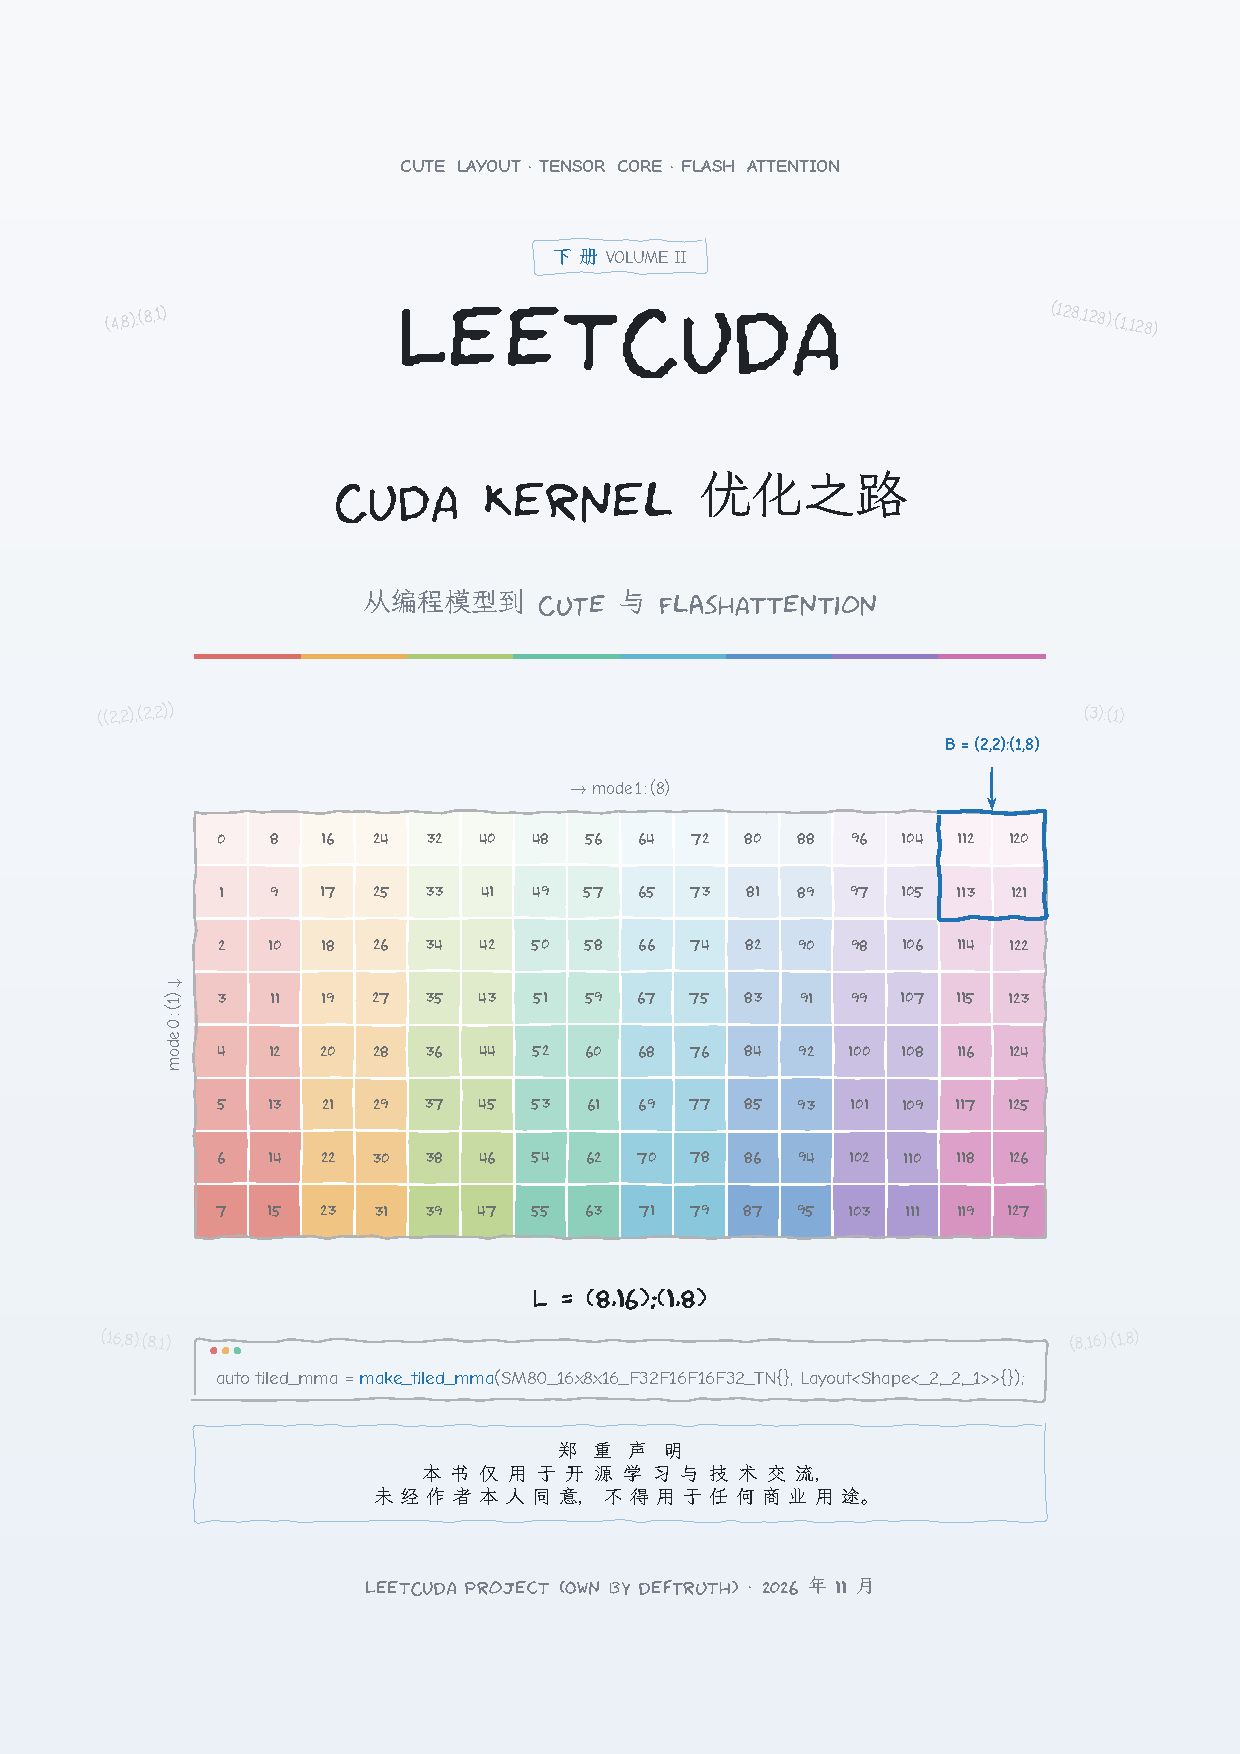
\includegraphics[width=\paperwidth,height=\paperheight]{figures/misc/cover-vol2.pdf}}}
\thispagestyle{empty}
\null
\clearpage

% 分册说明（主书不含此页）
\thispagestyle{empty}
\vspace*{0.18\textheight}
\begin{center}
  {\Large\bfseries 分册说明}\\[1.6em]
  \begin{minipage}{0.76\textwidth}
    \normalsize\linespread{1.4}\selectfont
    本书分上下两册。本册为\mbox{\textbf{下册}}，自 CuTe 篇后半起，收录第 24--45 章
    与附录 A--E：CuTe 篇后半、FP8/FP4 GEMM 篇、FP8/FP4 Attention 篇、SVDQuant 篇、
    CUTLASS Collective API 与附录。\mbox{\textbf{上册}}收录第 1--23 章。\par\vspace{1em}
    两册沿用全一册版的章号、图号、表号与公式编号，正文中的交叉引用可跨册对照。
  \end{minipage}
\end{center}
\clearpage

% 消除 frontmatter 的奇数开页空页，目录紧跟封面/说明
\begingroup
\let\cleardoublepage\clearpage
\frontmatter
\tableofcontents
\endgroup

% openany 电子书不强制右页起始：否则目录尾后 \mainmatter 的 \cleardoublepage 会补一页空白
\let\cleardoublepage\clearpage
\mainmatter

% 章号/部分号接续上册（上册含 23 个编号章、4 个部分；ch19b 为不编号导读）。
% 切点取「第二十四章」之前（两册各 341 页，实测），第四部分因此被切开：它的标题页在上册，
% 这里补一页不带编号的「第四部分（续）」并写进目录。\part* 自己不进目录、也不动 part 计数器，
% 所以 \addcontentsline 必须手写，且要放在 \clearpage 之后——页码才落在续页本身。
\setcounter{part}{4}
\setcounter{chapter}{23}

\clearpage
\phantomsection
\addcontentsline{toc}{part}{第四部分（续）：CuTe 篇}
\part*{第四部分（续）\\CuTe 篇：布局代数与现代化 Kernel 工程}
% ch23-cute-swizzle-tma.tex — CuTe（四）：Swizzle 与 TMA（RFC-F，2026-09-11）
% \url 由 book.tex 的 hyperref 提供；单章独立编译时降级为可断行的 \ttfamily
% （逐字符插入 \allowbreak，避免长 URL 造成 Overfull \hbox）
\makeatletter
\providecommand{\urlchbrk}[1]{\@tfor\next:=#1\do{\next\allowbreak}}
\makeatother
\providecommand{\url}[1]{{\ttfamily\urlchbrk{#1}}}
\chapter{CuTe（四）：Swizzle 与 TMA}\label{ch:23}

\section{本章导读}

第~\ref{ch:12}~章用一次 XOR 消除了 smem 的 bank conflict：把列块索引换成
列块 XOR 行号，即 \texttt{swizzle\allowbreak{}<64>\allowbreak{}(row,\allowbreak{} k)}。在那章的语境里它是一个
\emph{地址技巧}；可一旦同一段 kernel 里出现了 TMA、fp8、多级 tile 与多
stage 缓冲，同样的技巧就要同时回答三个新问题：它到底是什么形式的
数学对象、怎么和形状 $+$ 步长复合、怎么与硬件自己做的 swizzle 对齐。
本章把这三件事摊开。

\textbf{前置章节}：第~\ref{ch:12}~章（XOR swizzle 的银行冲突推导与手写
\texttt{swizzle<>} 家族）、第~\ref{ch:20}~章（Layout 代数与
\texttt{composition}）、第~\ref{ch:21}~章（Tensor 与 TiledCopy）、
第~\ref{ch:22}~章（TiledMMA）。本章是 Part~IV\textbf{CuTe 应用篇}的第二章，
不引入新的 CuTe 抽象，只把已有的 \texttt{Layout}/\texttt{Tensor} 用到
swizzle 与 TMA 两个难点上。

\textbf{源码区间}：hgemm.cuh L1232--1270，即 Phase~7c 的 smem 布局定义
（\texttt{Smem\allowbreak{}Layout\allowbreak{}Atom/\allowbreak{}SmemLayoutA/\allowbreak{}SmemLayoutB} 的定义
及其上方的位级注释）。为了给出 TMA 一侧的完整链路，本章还引用：
hgemm.cuh L1859--2100（宏块 \texttt{NOTES\_\allowbreak{}V2\_\allowbreak{}ENABLE\_\allowbreak{}TMA\_\allowbreak{}MMA\_\allowbreak{}WS}
内的 kernel \texttt{hgemm\_\allowbreak{}tma\_\allowbreak{}mma\_\allowbreak{}ws\_\allowbreak{}tn}：模板参数、对齐约定、
生产者/消费者两侧的 swizzle 地址算术）、common.cuh L262--350（本仓库自带的
\texttt{SwizzleBMS} 位级镜像与 kColStride 映射表）、bench/flash\_attn.cu L79--85
（\texttt{make\_\allowbreak{}tma\_\allowbreak{}copy} 的最小用法）。\textbf{编译宏}：
\texttt{NOTES\_\allowbreak{}V2\_\allowbreak{}ENABLE\_\allowbreak{}CUTE}（CuTe 布局部分）与
\texttt{NOTES\_\allowbreak{}V2\_\allowbreak{}ENABLE\_\allowbreak{}TMA\_\allowbreak{}MMA\_\allowbreak{}WS}（TMA 部分，需要
\texttt{CUtensorMap} 与 \texttt{cuda::\allowbreak{}barrier}，TMA tensor 指令需要
sm90 及以上；具体 kernel 还受 \texttt{\_\_CUDA\_ARCH\_\_} 分支约束）。

配套最小测试 \texttt{book/\allowbreak{}tests/\allowbreak{}ch23\_\allowbreak{}swizzle\_\allowbreak{}tma.cu} 是一个\emph{纯主机侧}
断言程序：它把本章的全部公式（位级 XOR、chunk 置换、复合语义、
\texttt{tile\_\allowbreak{}to\_\allowbreak{}shape} 的重复规律、SW128 atom 的物理排布）逐条与 CuTe 的
布局求值结果做数值对照。这些断言与 sm\_120a 上实测的 TMA 硬件行为一致
（对照数据见测试 case E 的硬件对照）。

\section{问题与动机}

第~\ref{ch:12}~章那行 swizzle 在真实工程里有三种走样形态。

\textbf{走样一：语义只存在于调用点。} 手写版的 swizzle 是一个自由函数，
调用点写 \texttt{swizzle\allowbreak{}<64>\allowbreak{}(row,\allowbreak{} k)}，函数体里写死取 bit7--9（3 位）、
右移 3 位后 XOR 到 bit4--6。要换 fp8（元素 1 字节、行宽翻倍）或换行宽（64 B/128 B/256 B），
就得改函数体内的位域，而改对与否只能靠再跑一遍正确性测试。ch12 的 kernel
之所以只写了一个 \texttt{swizzle<>}，是因为它只有一个 smem 布局。

\textbf{走样二：与其它维度的耦合。} 上一章的 smem 需要三层结构：
$B_M\times B_K$ 的 tile、$k_{\text{stage}}$ 个 stage、以及 scale 因子等
旁路数据。手写版的地址表达式把这些维度乘在一起
（\texttt{base + stage * BM * BK + row * BK + swizzle\allowbreak{}(row,\allowbreak{} k)}），
每加一层就要重新推导一次谁在 swizzle 内部、谁在外部。第~\ref{ch:12}~章
末尾那个 \texttt{k\_step} 要不要放进 \texttt{swizzle\allowbreak{}<k\allowbreak{}Mma\allowbreak{}K>} 参数的问题，
本质就是复合顺序问题。

\textbf{走样三：与硬件 swizzle 的一致性。} TMA 的
\texttt{cp.\allowbreak{}async.\allowbreak{}bulk.\allowbreak{}tensor} 由硬件按 descriptor 里声明的模式
（\texttt{CU\_\allowbreak{}TENSOR\_\allowbreak{}MAP\_\allowbreak{}SWIZZLE\_\allowbreak{}32B/\allowbreak{}64B/\allowbreak{}128B}）自己把 gmem 的数据
摆进 smem。此时 smem 里的物理排布由\emph{硬件}决定，软件只能去对齐它：
要么用同一套位公式算地址（本章的 \texttt{swizzle<64>} 路径），要么把
swizzle 编码进基址（WGMMA descriptor 的 \texttt{base\_offset} 字段，
见第~\ref{ch:13}~章）。

一旦两边的模式不一致，结果不是略微掉精度，
而是整块 tile 错位。这类错误在 hgemm.cuh~L1899--1917 的注释里被写成
一条硬性约定：本路径使用 128\,B swizzle，因此 TMA smem 基址必须
1024\,B 对齐，否则 phase 不为零，消费者算出来的地址全错。经典三档的
对齐要求并不相同，32/64/128\,B 模式分别为 256/512/1024\,B，见常见坑。

本章要证明的是：CuTe 把这三个走样各自收进了一个可检验的对象：
\texttt{Swizzle\allowbreak{}<B,\allowbreak{}M,\allowbreak{}S>}（位语义）、\texttt{composition}（复合语义）、
\texttt{tile\_\allowbreak{}to\_\allowbreak{}shape}（多级扩展），而 TMA 侧则用
\texttt{make\_\allowbreak{}tma\_\allowbreak{}copy} 把 gmem 张量与 smem 布局一次性编码成硬件
descriptor。理解这三样东西的边界（尤其是它们\emph{不能}保证什么）。

\section{数学原理}

\subsection{现象：bank conflict 与两种解法}

shared memory 被切成 32 个 bank（每个 4\,B 宽），一个
warp 的 32 个线程如果同时访问落在同一 bank 的多个地址，硬件只能把它们串行
化，这就是 bank conflict。GEMM 的 smem tile 是 $8$ 行 $\times 64$ 列的 fp16
（一行 $64\times2=128$\,B），\texttt{ldmatrix} 让每个线程负责一根 $16$\,B 的
行段（8 个 half，横跨 4 个 bank）。按最自然的行优先、行步长 $128$\,B
摆放，第 $r$ 行第 $j$ 个 $16$\,B 块的起始字节是 $128r+16j$，它落在 bank

\begin{equation}
  \label{eq:23-bank}
  \mathrm{bank}(r,j) = \frac{128r+16j}{4} \bmod 32 = (32r + 4j) \bmod 32
  = 4j \bmod 32 ,
\end{equation}

行号 $r$ 被 $32r$ 项消掉了：同一个列块 $j$ 在 8 行里全部落在相同的
4 个 bank 上，8 个线程排队等待，构成 8-way conflict。

朴素解法：padding。每行尾部补 8 个 half（行宽从 $64$ 变 $72$ 个
元素，即 $144$\,B），行步长不再是 128 的倍数，$r$ 重新参与取模，冲突消失。

代价有四条。$12.5\%$ 的容量被浪费；行宽不再是 $2^{M+S}$ 字节的标准形态。
后面会看到，TMA 硬件只认标准形态，padding 方案无法用于 TMA。每次换元素类型或
$B_K$ 都要重新推一遍补偿量。

置换解法：XOR。保持行宽不动，把\emph{列块索引}换成\textbf{块索引 XOR
行号}：第 $r$ 行的逻辑块 $j$ 搬到物理位置 $j\oplus r$。固定列块扫 8 行，
物理块取遍 $0..7$ 的 8 个不同值，8 根 $16$\,B 段各落一处 bank 组，冲突
消失，容量零浪费。

@reed《cute 之 Swizzle》正是从\textbf{逻辑矩阵位置与 bank 的
对应关系}出发讲这件事。这里要区分两条硬件路径：TMA 由 descriptor
声明硬件 swizzle 模式；\texttt{ldmatrix} 没有原生 swizzle 操作数，只接收
每 lane 地址，XOR 必须由软件地址计算完成。成因与两种解法的
三面板对照见图~\ref{fig:23-bank-conflict}。

\begin{figure}[H]
\centering
\begin{tikzpicture}[font=\tiny]
  \definecolor{bkred}{RGB}{192,45,45}
  \begin{scope}
    \foreach \fr in {0,...,7}{
      \foreach \fc in {0,...,7}{
        \pgfmathtruncatemacro{\gl}{8+9*\fc}
        \node[fill=gray!\gl, minimum width=0.4cm, minimum height=0.4cm, inner sep=0pt]
          at ({(\fc+0.5)*0.4},{-(\fr+0.5)*0.4}) {\fc};
      }
    }
    \draw[thin] (0,0) grid[xstep=0.4cm, ystep=0.4cm] (3.2,-3.2);
    \draw[tkOrange, very thick] (0,0) rectangle (3.2,-3.2);
    \draw[bkred, very thick] (0,0) rectangle (0.4,-3.2);
    \foreach \fr in {0,...,7}{
      \node[anchor=east] at (-0.06,{-\fr*0.4-0.2}) {\fr};
    }
    \node[anchor=east, font=\tiny, rotate=90] at (-0.42,-1.6) {行 $r$};
    \node[anchor=south, font=\tiny] at (1.6,0.32) {列块 $j$};
    \node[anchor=south, font=\scriptsize\bfseries, text=tkOrange] at (1.6,0.62)
      {(a) 无 swizzle（行步长 128\,B）};
    \node[anchor=north, font=\tiny, align=center] at (1.6,-3.35)
      {$\mathrm{bank}(r,j)=4j\bmod32$：行号被 $32r$ 项消掉，\\
       同一列块 8 行同组（红框列：8 线程排队）$\to$ \textbf{8-way}};
  \end{scope}
  \begin{scope}[shift={(4.7,0)}]
    \foreach \fr in {0,...,7}{
      \foreach \fc in {0,...,7}{
        \pgfmathtruncatemacro{\gb}{mod(\fr+\fc,8)}
        \pgfmathtruncatemacro{\gl}{8+9*\gb}
        \node[fill=gray!\gl, minimum width=0.4cm, minimum height=0.4cm, inner sep=0pt]
          at ({(\fc+0.5)*0.4},{-(\fr+0.5)*0.4}) {\gb};
      }
      \node[pattern=north east lines, pattern color=gray!55,
        minimum width=0.4cm, minimum height=0.4cm, inner sep=0pt]
        at (3.4,{-(\fr+0.5)*0.4}) {};
    }
    \draw[thin] (0,0) grid[xstep=0.4cm, ystep=0.4cm] (3.2,-3.2);
    \draw[thin] (3.2,0) grid[xstep=0.4cm, ystep=0.4cm] (3.6,-3.2);
    \draw[tkBlue!70, very thick] (0,0) rectangle (3.6,-3.2);
    \draw[thick] (3.2,0) -- (3.2,-3.2);
    \node[anchor=south, font=\tiny] at (3.4,0.12) {pad};
    \node[anchor=south, font=\scriptsize\bfseries, text=tkBlue] at (1.8,0.62)
      {(b) padding（行步长 144\,B）};
    \node[anchor=north, font=\tiny, align=center] at (1.8,-3.35)
      {组号 $=(r{+}j)\bmod8$ 逐行错位：冲突消失；代价 $12.5\%$ 容量浪费，\\
       行宽非 $2^{M+S}$ 标准形态，TMA 不支持};
  \end{scope}
  \begin{scope}[shift={(9.7,0)}]
    \foreach \fr in {0,...,7}{
      \foreach \fc in {0,...,7}{
        \pgfmathtruncatemacro{\gc}{mod(mod(\fc,2)+mod(\fr,2),2)
          + 2*mod(int(\fc/2)+int(\fr/2),2)
          + 4*mod(int(\fc/4)+int(\fr/4),2)}
        \pgfmathtruncatemacro{\gl}{8+9*\gc}
        \node[fill=gray!\gl, minimum width=0.4cm, minimum height=0.4cm, inner sep=0pt]
          at ({(\fc+0.5)*0.4},{-(\fr+0.5)*0.4}) {\gc};
      }
    }
    \draw[thin] (0,0) grid[xstep=0.4cm, ystep=0.4cm] (3.2,-3.2);
    \draw[tkGreen, very thick] (0,0) rectangle (3.2,-3.2);
    \node[anchor=south, font=\scriptsize\bfseries, text=tkGreen] at (1.6,0.62)
      {(c) XOR swizzle（行步长 128\,B）};
    \node[anchor=north, font=\tiny, align=center] at (1.6,-3.35)
      {物理块 $j\to j\oplus r$ 对角散布：同列 8 格 8 组；\\
       容量零浪费，代价仅 1 条 \texttt{LOP3}（式~\eqref{eq:23-chunk} 的前身）};
  \end{scope}
  \node[anchor=north, font=\tiny] at (6.5,-4.5)
    {格内数字 $=$ bank 组号、灰度按组号渐变（0 浅 $\to$ 7 深）；每格 $=$ 一个
     16\,B chunk $=$ 4 个 bank；三面板共用行轴 $r$（8 行）};
\end{tikzpicture}
\caption{bank conflict 成因与两种解法（式~\eqref{eq:23-bank}）：8 行
$\times$ 8 chunk 的 fp16 smem tile，每格为一个 16\,B chunk（占 4 个
bank），格内数字为 bank 组号、灰度按组号渐变。(a) 无 swizzle：
$\mathrm{bank}(r,j)=4j\bmod32$——行号被 $32r$ 项消掉，同一列块 8 行同组
（红框列 8 线程串行化）$\to$ 8-way conflict；(b) padding：行宽 144\,B 使
$r$ 重新参与取模（组号 $=(r+j)\bmod8$ 逐行错位，冲突消失），代价是
$12.5\%$ 容量浪费且行宽非 $2^{M+S}$ 标准形态——无法用于 TMA；(c) XOR
swizzle：物理块 $j\to j\oplus r$ 对角散布，同列 8 格 8 组，容量零浪费、
代价仅 1 条 \texttt{LOP3}。}
\label{fig:23-bank-conflict}
\end{figure}

剩下的问题是把这个技巧写成可复用、可组合的类型。这是
\texttt{Swizzle\allowbreak{}<B,\allowbreak{}M,\allowbreak{}S>} 的职责，也是 3.2--3.6 节的主题。

\subsection{Swizzle 的位模型}

CuTe 的 \texttt{Swizzle\allowbreak{}<B,\allowbreak{}M,\allowbreak{}S>} 只做一件事：对一个整数做位域置换。
把上面的 XOR 一般化：取 offset 中一段连续 $B$ 位（\textbf{源字段}），
右移 $S$ 位后 XOR 到另一段连续 $B$ 位（\textbf{目标字段}）上，两段之间的
$M$ 位（块内偏移）原样保留。\texttt{cute/\allowbreak{}swizzle.\allowbreak{}hpp} 给出的位图是

\begin{equation}
\label{eq:23-bits}
\underbrace{\texttt{xxxxxxx}\cdots\texttt{x}}\sb{\text{高位}}
\underbrace{\texttt{YYY}}\sb{\text{源}} \underbrace{\texttt{xxxxxxx}}\sb{\text{不变}}
\underbrace{\texttt{ZZZ}}\sb{\text{目标}} \underbrace{\texttt{xxxx}}\sb{\text{M 位}}
\end{equation}

其中 \texttt{ZZZ} 落在 bit $[M, M+B)$，\texttt{YYY} 落在 bit
$[M+S, M+S+B)$（$S>0$ 时）。求值是把 \texttt{YYY} 段右移到
\texttt{ZZZ} 段再做 XOR：

\begin{align}
\label{eq:23-masks}
\text{yyy\_msk} &= ((1\ll B)-1) \ll (M+\max(0,S)), \\
\label{eq:23-zzz}
\text{zzz\_msk} &= ((1\ll B)-1) \ll (M-\min(0,S)), \\
\label{eq:23-apply}
\text{apply}(\text{off}) &= \text{off} \oplus \left(\text{off} \wedge
\text{yyy\_msk}\right) \gg S .
\end{align}

这个定义有三个立刻可用的性质，它们是后面一切讨论的基础。

\textbf{(a) 对合性。} 设 $y=\text{off}\wedge\text{yyy\_msk}$。式~\eqref{eq:23-apply}
只改 \texttt{ZZZ} 段，\texttt{YYY} 段原封不动，所以第二次求值时
$y$ 不变、$y\gg S$ 不变，XOR 两次即还原：$\text{apply}(\text{apply}(x))=x$。
Swizzle 是置换群里的对合元，这是它能当布局用的前提。

\textbf{(b) 实现代价。} 式~\eqref{eq:23-apply} 的算术量是
1 次 AND、1 次移位、1 次 XOR，映射到 SASS 就是一条 \texttt{LOP3}
或两条整数指令。相对之下，任何查表 $+$ 分支的地址重排方案都会引入
warp 内不一致的延迟。TMA 可以把相应模式编码进 descriptor；
\texttt{ldmatrix} 路径则由软件把这几次位运算折叠进每 lane 的地址计算，
而不是由指令本身执行 swizzle。

\textbf{(c) 约束 $|S|\ge B$。} CuTe 在构造时会静态断言
\texttt{abs(SShift) >= BBits}（common.cuh~L291 的镜像实现抄了同一条）。
若 $|S|<B$，\texttt{YYY} 与 \texttt{ZZZ} 在位上重叠，XOR 会把源字段
自己改掉，对合性立刻失效，读写用同一公式这一工程前提也就没了。

\begin{table}[htbp]
\centering
\caption{三个标准档位与 TMA 硬件模式、第~\ref{ch:12}~章手写版的对应关系
（周期 $=2^{M+S+B}$ 字节，$2^M$ 字节 $=16$\,B $=8$ 个 fp16；末行
\texttt{<3,3,3>} 为元素口径，周期 $512$ 个元素折算 $1024$\,B）。}
\label{tab:23-modes}
\begin{tabular}{cccccc}
\toprule
$B$ & $M$ & $S$ & 周期（字节） & TMA descriptor 模式 & 第~\ref{ch:12}~章手写版 \\
\midrule
1 & 4 & 3 & 256  & \texttt{SWIZZLE\_32B}  & \texttt{swizzle<16>} \\
2 & 4 & 3 & 512  & \texttt{SWIZZLE\_64B}  & \texttt{swizzle<32>} \\
3 & 4 & 3 & 1024 & \texttt{SWIZZLE\_\allowbreak{}128\allowbreak{}B} & \texttt{swizzle<64>} \\
3 & 3 & 3 & 1024 & 无对应模式 & 无 \\
\bottomrule
\end{tabular}
\end{table}

\subsection{从位模型到 chunk XOR 行号}

表~\ref{tab:23-modes} 最后一个档位 \texttt{Swizzle\allowbreak{}<3,\allowbreak{}3,\allowbreak{}3>} 值得单独说：
它在 CuTe 文档里最常出现（因为文档的例子用 fp32），但它与
\texttt{SWIZZLE\_\allowbreak{}128\allowbreak{}B} 不是同一件事，区别在偏移量的单位。
若偏移量是\emph{元素索引}且元素为 fp16，那么 $M=3$ 意味着低 3 位不变
$=$ 每 8 个元素（$=$ 16 B）一组的块内偏移不变；$M=4$ 则意味着低 4 位不变
$=$ 每 $2^4=16$ 个\emph{元素}（$=$ 32 B，fp16 下过于粗）不变。硬件模式的
定义永远落在字节上：三档的 XOR 粒度统一是 16\,B（$M=4$ 决定），
差别在 XOR 位数（$B=1/2/3$）与行宽（32/64/128\,B）。于是

\begin{itemize}[leftmargin=2em]
\item 偏移量按元素计（fp16）：SW128 $=$ \texttt{Swizzle\allowbreak{}<3,\allowbreak{}3,\allowbreak{}3>}；
\item 偏移量按字节计：SW128 $=$ \texttt{Swizzle\allowbreak{}<3,\allowbreak{}4,\allowbreak{}3>}。
\end{itemize}

两者的位公式是同一个式子在不同单位下的写法。把它写成行宽 $2^{M+S}$ 字节、
块宽 $2^M$ 字节的一般形式（$R$ 为行索引）：

\begin{equation}
\label{eq:23-chunk}
\text{phys} = \text{off} \oplus \left(\left(R \wedge (2^B-1)\right)
\ll M\right),
\qquad \text{即}\quad \text{chunk}' = \text{chunk} \oplus R .
\end{equation}

式~\eqref{eq:23-chunk} 是本章最有用的一条：\textbf{凡是行宽恰好等于
$2^{M+S}$ 字节的布局，swizzle 的物理效果就是 16 B 块的列号 XOR 行号}。
它把位运算的抽象还原成第~\ref{ch:12}~章那张对角线置换的图。
验证方式不是直接对 \texttt{GMMA::\allowbreak{}Layout\_\allowbreak{}K\_\allowbreak{}SW128\_\allowbreak{}Atom\allowbreak{}<half>}
的 \texttt{layout(r,c)} 求值，而是把 \texttt{Swizzle<3,4,3>} 作用在
\textbf{字节地址}上，逐点比较
$64r+8\cdot((c/8)\oplus(r\bmod 8))+(c\bmod 8)$
（第~\ref{sec:23-minitest}~节的 case C/E1/E2，4096 点全中）。
GMMA 原子是位置相关的 smem 指针语义，裸 \texttt{layout(r,c)} 只有
$1024/4096$ 命中；把它当普通 layout 与硬件 swizzle 逐点比会误判
（case E3 明确断言了这一非等价）。

\paragraph{实践须知}（参数与单位绑定，抄参数前先确认单位）
\begin{itemize}
  \item \textbf{同一个 \texttt{Swizzle} 类型在不同单位下对应不同的物理块宽}。
        CuTe 文档与许多教程演示 \texttt{Swizzle\allowbreak{}<3,\allowbreak{}3,\allowbreak{}3>} 用的位公式是
        $\text{offset}'=\text{offset}\oplus((\text{offset}\wedge
        (\texttt{0b111}\ll6))\gg3)$，掩码落在 bit $[6,9)$，这是把偏移量
        按\emph{字节}读的口径，物理上是 $8$\,B 块、$64$\,B 行的置换。
        换到 fp16 的 SW128：块宽必须是 $16$\,B $=8$ 个元素，于是偏移量
        按\emph{元素}计时 \texttt{Swizzle\allowbreak{}<3,\allowbreak{}3,\allowbreak{}3>}（hgemm.cuh 用的就是它）、
        按\emph{字节}计时 \texttt{Swizzle\allowbreak{}<3,\allowbreak{}4,\allowbreak{}3>}（CUTLASS 的 GMMA 原子
        用的是后者）。
  \item 行宽必须与参数自洽。式~\eqref{eq:23-chunk} 的前提是行宽
        $=2^{M+S}$ 字节：fp16 的 $64$ 列恰是 $128$\,B，对应 SW128 的
        \texttt{<3,4,3>}（字节口径）；若 tile 的行宽只有 $64$\,B（fp16 的
        $32$ 列），直接套用 SW128 参数只能得到强度减半的置换，
        见 4.1 节的实测。
\end{itemize}

\subsection{composition：Swizzle 与基础布局的合成}

CuTe 用 \texttt{composition} 把 Swizzle 与基础布局合成一个整体：

\begin{equation}
\label{eq:23-comp}
R = \texttt{comp}\big(\text{Swizzle},\ \text{Offset},\ \text{Layout}\big),
\qquad R(c) = \text{Swizzle}\Big(\text{Offset} + \text{Layout}(c)\Big).
\end{equation}

注意式~\eqref{eq:23-comp} 的自变量是坐标，而 Swizzle 作用在
偏移量上，中间隔着一次 \texttt{Layout} 求值：
坐标体系不用变，物理地址已经换了，之后的代码无需改动。
仍用 $(r,c)$ 问第 $r$ 行第 $c$ 列在哪，布局会换算成被置换过的
物理 offset；读写两侧只要用同一个布局别名，改写永远自洽。hgemm.cuh 的
smem 原子就是这一步的实例：

\lstinputlisting[linerange={1244-1266},firstnumber=auto,
  title={hgemm.cuh L1244-1266（swizzle 语义注释 $+$ SmemLayoutAtom 与布局三件套）}]{../hgemm.cuh}

这段注释里有两处要带着式~\eqref{eq:23-chunk} 去读：一是它把 $S=3$ 解释成
\textbf{$2^3=8$ 个基本元素组成一行，即 128 bytes}，二是它声称\textbf{$8\times32$ 的
逻辑 tile 正好对应 8 行 $\times$ 128\,B}。结论（chunk XOR 行号）没错，
但它描述的行宽与紧随其后的 base layout \texttt{\allowbreak{}(8,\allowbreak{}32):\allowbreak{}(32,\allowbreak{}1)} 并不一致：
32 个 fp16 只有 64\,B。行宽不足会让 swizzle 的实际强度降低，
4.1 节的实践须知给出实测。

\subsection{位置无关与位置相关：最容易出错的一处}

Swizzle 是地址的函数，所以必须先回答：这个地址从哪来？CuTe 给了两条
路径。\texttt{cute/\allowbreak{}pointer\_\allowbreak{}swizzle.\allowbreak{}hpp} 的 L44--46 注释把区别写得很清楚：

\begin{lstlisting}[style=console]
as the offset. That means that swizzle_layout will implement
position-independent swizzle layouts, while swizzle_ptr implements
position-dependent swizzle tensors. Arch chose to design hardware with
position-dependent swizzles.
\end{lstlisting}

\begin{itemize}[leftmargin=2em]
\item \textbf{位置无关（layout）}：$R(c)=\text{Swizzle}(\text{Layout}(c))$，
Swizzle 只看布局内部的偏移量，与这段内存在 smem 里的绝对位置无关。
\texttt{layout(c)} 是纯函数，可在主机侧求值、可参与类型推导。
\item \textbf{位置相关（pointer）}：Swizzle 作用在绝对地址上
（\texttt{apply\_\allowbreak{}swizzle} 内部是 \texttt{reinterpret\_\allowbreak{}cast\allowbreak{}<uintptr\_\allowbreak{}t>}），
所以同一条逻辑访问，在不同的 smem 基址下会落到不同的物理位置。
\end{itemize}

硬件选的是后者。这解释了 hgemm.cuh~L1899--1917 那条 1024 B 对齐的硬约定：
若基址低 10 位为零，\texttt{phase} 为零，位置相关与位置无关两种视角给出
相同的地址；若基址只有 128 B 对齐，硬件写进去的 phase 与软件算出来的
phase 不一致，读出来就是错的。

本章测试里有一条刻意分开的对照（case E）：把
\texttt{Swizzle\allowbreak{}<3,\allowbreak{}4,\allowbreak{}3>} 作用在字节偏移上得到的模式，
与 sw\_120a 上实测 TMA \texttt{SWIZZLE\_\allowbreak{}128\allowbreak{}B} 的 4096 个元素逐点相等
（$0$ 失配）。而用 \texttt{tile\_\allowbreak{}to\_\allowbreak{}shape} 得到的\emph{分块布局求值}
去对同一块 smem 时，4096 点里只有 1024 点（$25\%$）能对上。这 $25\%$
\textbf{不是}位置无关与位置相关的语义分界，而是\textbf{单位错配}：
裸求值把字节口径的 \texttt{Swizzle\allowbreak{}<3,\allowbreak{}4,\allowbreak{}3>} 直接作用在元素偏移上（缺了
fp16 元素到字节的 $\times2$ recast）。\texttt{YYY} 取到的是元素偏移的
bit$[7,10)$ 而非字节偏移的 bit$[7,10)$，仅当行号满足
$r\bmod 16\in\{0,2,4,6\}$（与列无关，占 $1/4$ 的行）时，两种口径取到的
XOR 位段相同、结果相等。

$1024/4096$ 正是这条规则的命中率
（数值模拟 64 行 $\times$ 64 列逐点核对）。补上 recast、按正确字节口径
求值，分块布局同样 $4096$ 点全部命中。基址对齐为什么是硬约束见
图~\ref{fig:23-phase-align}。

\begin{figure}[H]
\centering
\begin{tikzpicture}[font=\tiny]
  \definecolor{phaseRed}{RGB}{192,45,45}
  \definecolor{phaseGreen}{RGB}{39,120,62}
  \definecolor{phaseBlue}{RGB}{150,185,220}
  \definecolor{phaseSand}{RGB}{242,214,168}
  \foreach \bk in {0,...,11}{
    \ifnum\bk<4 \def\bfill{gray!15} \fi
    \ifnum\bk>3 \ifnum\bk<7 \def\bfill{phaseBlue} \fi \fi
    \ifnum\bk>6 \ifnum\bk<10 \def\bfill{phaseSand} \fi \fi
    \ifnum\bk>9 \def\bfill{gray!15} \fi
    \node[fill=\bfill, minimum width=0.42cm, minimum height=0.42cm, inner sep=0pt]
      at ({\bk*0.42+0.21},-0.21) {\bk};
  }
  \draw[thin] (0,0) grid[xstep=0.42cm, ystep=0.42cm] (5.04,-0.42);
  \draw[very thick] (0,0) rectangle (5.04,-0.42);
  \foreach \flda/\fldb/\fname in {0/4/块内偏移,4/7/ZZZ,7/10/YYY $=r$,10/12/高位}{
    \draw[thick] ({\flda*0.42},0.05) -- ({\flda*0.42},0.15)
      -- ({\fldb*0.42},0.15) -- ({\fldb*0.42},0.05);
    \node[anchor=south] at ({(\flda+\fldb)*0.21},0.18) {\fname};
  }
  \node[anchor=east] at (-0.1,-0.21) {字节地址};
  \foreach \cc in {0,...,7}{
    \pgfmathtruncatemacro{\swv}{1-mod(\cc,2)+2*(1-mod(int(\cc/2),2))+4*int(\cc/4)}
    \pgfmathtruncatemacro{\hwv}{mod(\cc,2)+2*mod(int(\cc/2),2)+4*(1-int(\cc/4))}
    \node[fill=tkFillBlue!60, minimum width=0.42cm, minimum height=0.42cm, inner sep=0pt]
      at ({\cc*0.42+0.21},-1.31) {\cc};
    \node[fill=tkFillBlue!60, minimum width=0.42cm, minimum height=0.42cm, inner sep=0pt]
      at ({\cc*0.42+0.21},-1.91) {\swv};
    \node[fill=tkFillBlue!60, minimum width=0.42cm, minimum height=0.42cm, inner sep=0pt]
      at ({\cc*0.42+0.21},-2.51) {\swv};
    \node[fill=tkFillOrange!50, minimum width=0.42cm, minimum height=0.42cm, inner sep=0pt]
      at ({\cc*0.42+0.21},-3.51) {\cc};
    \node[fill=tkFillOrange!50, minimum width=0.42cm, minimum height=0.42cm, inner sep=0pt]
      at ({\cc*0.42+0.21},-4.11) {\swv};
    \node[fill=tkFillOrange!50, minimum width=0.42cm, minimum height=0.42cm, inner sep=0pt]
      at ({\cc*0.42+0.21},-4.71) {\hwv};
  }
  \foreach \ry in {-1.1,-1.7,-2.3,-3.3,-3.9,-4.5}{
    \foreach \kx in {0,...,8}{
      \draw[thin] ({\kx*0.42},\ry) -- ({\kx*0.42},{\ry-0.42});
    }
    \draw[thin] (0,\ry) -- (3.36,\ry);
    \draw[thin] (0,{\ry-0.42}) -- (3.36,{\ry-0.42});
  }
  \draw[phaseGreen, very thick] (0,-2.3) rectangle (3.36,-2.72);
  \draw[phaseRed, very thick] (0,-4.5) rectangle (3.36,-4.92);
  \node[anchor=east] at (-0.06,-1.31) {逻辑块号 $j$};
  \node[anchor=east] at (-0.06,-1.91) {位置无关：布局求值};
  \node[anchor=east] at (-0.06,-2.51) {位置相关：硬件相位};
  \node[anchor=east] at (-0.06,-3.51) {逻辑块号 $j$};
  \node[anchor=east] at (-0.06,-4.11) {位置无关：布局求值};
  \node[anchor=east] at (-0.06,-4.71) {位置相关：硬件相位};
  \node[anchor=west, phaseGreen] at (3.5,-2.51) {两视角同址};
  \node[anchor=west, phaseRed] at (3.5,-4.71) {两视角错位};
  \node[font=\scriptsize\bfseries] at (-2.3,-1.91) {(a)};
  \node[font=\scriptsize\bfseries] at (-2.3,-4.11) {(b)};
  \node[anchor=north west, align=left, text width=8.4cm] at (5.9,-1.15)
    {(a) 基址低 $10$ 位为零：绝对地址与 offset 的 bit$[4,7)$、bit$[7,10)$
     完全一致，硬件按 YYY 取到的行号就是布局里的 $r=3$，XOR 值同为
     $3$——两条路径落到同一 chunk。本章测试 case~E 的 $4096$ 点逐点相等
     就是这个前提。};
  \node[anchor=north west, align=left, text width=8.4cm] at (5.9,-3.35)
    {(b) 基址的 bit$7$ 非零：硬件在绝对地址上取行号，$r$ 被整体抬 $1$
     （模 $8$），XOR 值从 $3$ 变成 $4$——同一列 $8$ 个 chunk 全部错位，
     写进去和读出来不是同一批地址。};
  \node[anchor=north west, align=left, text width=15.5cm] at (0,-5.5)
    {结论：\texttt{Swizzle} 在 CuTe 里既能当\emph{位置无关}的布局
     （只作用在 offset 上）用，也会被硬件当\emph{位置相关}的置换
     （作用在绝对地址上）用。两条路径要一致，基址的低 $10$ 位就必须为零
     ——这就是 hgemm.cuh L1899--1917 把\textbf{TMA 路径 smem 基址 $1024$\,B
     对齐}写成硬约定的原因。WGMMA 一侧还有 descriptor 的
     \texttt{base\_offset}（bit$[49,52)$）可以事后补偿相位，
     \texttt{ldmatrix} 的地址通道没有这个补偿位。};
\end{tikzpicture}
\caption{位置无关与位置相关：为什么 TMA 路径要求 smem 基址 $1024$\,B
对齐（3.5 节）。上方把字节地址的位段摆开：bit$[4,7)$ 的 ZZZ 是 XOR
目标（$16$\,B 块号），bit$[7,10)$ 的 YYY 是源（行号 $r$）。(a) 基址低
$10$ 位为零时，绝对地址与 offset 的这两个字段一致，布局求值与硬件相位给
出同一个物理 chunk；(b) 基址一旦带 bit$7$，硬件看到的行号整体抬 $1$，
XOR 值随之改变，写/读两条路径错位。}
\label{fig:23-phase-align}
\end{figure}

\subsection{tile\_to\_shape：从原子到多级 smem 布局}

最后一个环节是把 $8\times B_K$ 的原子扩到 $B_M\times B_K\times k_{\text{stage}}$：

\begin{equation}
\label{eq:23-tile}
\texttt{tile\_\allowbreak{}to\_\allowbreak{}shape}(\text{atom}, (B_M,B_K,k_{\text{stage}}))
= \text{blocked product}\Big(\text{atom},\ \text{repeat counts}\Big).
\end{equation}

它有两个必须记住的行为。

\textbf{(1) 整除约束。} \texttt{tile\_\allowbreak{}to\_\allowbreak{}shape} 要求目标形状能被原子
形状整除；静态形状不满足时触发编译期 \texttt{static\_assert}
（\texttt{block shape does not divide the target shape}）。于是
$B_K=32$ 的 tile \emph{不可能}直接套 $8\times64$ 的 SW128 原子；
反过来，$8\times32$ 的原子能铺 $B_K=32$，却也不是 SW128 的标准形态。

\textbf{(2) 重复原子并保留复合结构。} 实测
\texttt{tile\_\allowbreak{}to\_\allowbreak{}shape\allowbreak{}(SW128\_\allowbreak{}atom,\allowbreak{} (64,\allowbreak{}64))} 的类型打印为
\texttt{Sw\allowbreak{}<3,\allowbreak{}4,\allowbreak{}3> o ... o \allowbreak{}(\allowbreak{}(8,\allowbreak{}8),\allowbreak{}(64,\allowbreak{}1)):\allowbreak{}(\allowbreak{}(64,\allowbreak{}512),\allowbreak{}(1,\allowbreak{}0))}。
这里的 stride 0 位于第二个顶层 mode 的 size-1 子 mode：$(64,1){:}(1,0)$，
不是“宽度轴偏移已由 swizzle 字段承载”。

工程上不要把这个复合布局当 flat 偏移公式手算地址（见 3.5 节的语义分界），
要读 smem 就用 \texttt{make\_tensor} 构造张量。带 swizzle 的
\texttt{Composed\allowbreak{}Layout} 不能用普通仿射布局的单一 \texttt{stride()} 接口完整表达，
所以该接口被删除；应分别读取 \texttt{layout\_a()}（swizzle）与
\texttt{layout\_b()}（基础布局）。本章测试的 case G 用 C++20 concept
在编译期检查这条 API 边界。

\section{设计与实现}

\subsection{hgemm 的三个 smem 布局别名}

Phase~7c 的 CuTe kernel 只用了三个布局别名（见式~\eqref{eq:23-comp} 引出的
那段代码：\texttt{Smem\allowbreak{}Layout\allowbreak{}Atom} 与由它派生的 \texttt{Smem\allowbreak{}Layout\allowbreak{}A/\allowbreak{}B}）：

逐项读：\texttt{composition\allowbreak{}(Swizzle\allowbreak{}<3,\allowbreak{}3,\allowbreak{}3>,\allowbreak{} base)} 里 base 是
$(8,32){:}(32,1)$，$T=$ \texttt{half}，所以偏移量以元素计，$M=3$ 对应
16\,B 块；\texttt{tile\_\allowbreak{}to\_\allowbreak{}shape} 把原子沿 $B_M$（128）、$B_K$（32）与
$k_{\text{stage}}$ 三个方向重复，得到 A 用的 $(B_M,B_K,2)$ 与 B 用的
$(B_N,B_K,2)$。cosize 分别是 $128\times32\times2=8192$ 与
$256\times32\times2=16384$ 个 half。这两个别名随后被
\texttt{make\_\allowbreak{}tensor\allowbreak{}(make\_\allowbreak{}smem\_\allowbreak{}ptr\allowbreak{}(.\allowbreak{}.\allowbreak{}.\allowbreak{}),\allowbreak{} Smem\allowbreak{}Layout\allowbreak{}A\{\})} 变成真正的
\texttt{Tensor}，从此所有地址算术都由 CuTe 完成，包括
\texttt{ldmatrix} 的每 lane 地址。

\paragraph{实践须知}（两处与注释核对过的实测）
\begin{itemize}
  \item \textbf{$8\times32$ 原子的实际强度只有一半。}把 $x=32r+c$（元素
        偏移）代入 \texttt{Swizzle\allowbreak{}<3,\allowbreak{}3,\allowbreak{}3>} 的位公式：掩码落在
        bit$\,[6,9)$，而 $32r$ 只贡献到 bit$\,5$ 起的位：行号的最
        低位落在源字段之外，真正参与 XOR 的只有 $r$ 的高两位，等价于
        $\text{chunk}'=\text{chunk}\oplus(r\gg1)$。XOR 值集合只有
        $\{0,8,16,24\}$ 四种；相邻两行共享同一图样，8 行一周期，共 4 种
        图样（理想 SW128 是逐行变化的 8 种图样，强度减半）。注释宣称的\textbf{8 行 $\times$ 128\,B、覆盖 32 bank}描述的是
        \texttt{Swizzle\allowbreak{}<3,\allowbreak{}3,\allowbreak{}3>} 配 $B_K=64$ 的形态。\textbf{该差异不影响
        正确性}，读写两侧用的是同一个布局别名，只是 bank 收益比注释口径
        小一半；本章测试 case F 逐点验证了这个退化形态
        （图~\ref{fig:23-sw-degenerate}）。
  \item \textbf{换行宽时的参数映射，看 common.cuh 的镜像实现。}
        common.cuh 的 \texttt{Swizzle\allowbreak{}BMS\allowbreak{}<B,\allowbreak{}M,\allowbreak{}S>} 是 \texttt{cute::\allowbreak{}Swizzle}
        位公式的镜像，其 \texttt{kColStride} 映射给出工程速查口径：列步长
        $16/32/64$（fp16 元素）分别对应 $(B,M,S)=(1,4,3)/(2,4,3)/(3,4,3)$，
        即 TMA 的 32/64/128\,B 三档（该实现对 $16/32/64$ 与手写版 bit-exact
        一致，host 端有等价性测试）。legacy 的 \texttt{kColStride}=8 无
        对应的 CuTe 标准模式，代码显式回退到手写 XOR 路径。\textbf{行宽一
        改，$B$ 与 $M$ 要一起改}，这就是 3.3 节实践须知里参数与单位绑定
        的具体体现。
\end{itemize}

\begin{figure}[H]
\centering
\begin{tikzpicture}[font=\tiny]
  \begin{scope}
    \foreach \rr in {0,...,7}{
      \foreach \cc in {0,...,3}{
        \pgfmathtruncatemacro{\xr}{int(\rr/2)}
        \pgfmathtruncatemacro{\xa}{mod(mod(\cc,2)+mod(\xr,2),2)}
        \pgfmathtruncatemacro{\xb}{mod(int(\cc/2)+int(\xr/2),2)}
        \pgfmathtruncatemacro{\phys}{\xa+2*\xb}
        \ifcase\xr
          \def\cff{colorx4!18}%
        \or
          \def\cff{colorx5!32}%
        \or
          \def\cff{colorx6!46}%
        \else
          \def\cff{colorx7!60}%
        \fi
        \node[fill=\cff, minimum width=0.62cm, minimum height=0.46cm, inner sep=0pt]
          at ({\cc*0.62+0.31},{-\rr*0.46-0.23}) {\phys};
      }
      \node[anchor=east] at (-0.06,{-\rr*0.46-0.23}) {\rr};
    }
    \draw[thin] (0,0) grid[xstep=0.62cm, ystep=0.46cm] (2.48,-3.68);
    \draw[very thick] (0,0) rectangle (2.48,-3.68);
    \foreach \pp in {0,...,3}{
      \pgfmathsetmacro{\ytop}{-0.92*\pp}
      \pgfmathsetmacro{\ybot}{-0.92*\pp-0.92}
      \draw[thick] (-0.3,\ytop) -- (-0.46,\ytop) -- (-0.46,\ybot) -- (-0.3,\ybot);
      \node[anchor=east] at (-0.52,{\ytop-0.46}) {$\oplus\,8{\cdot}\pp$};
    }
    \node[anchor=south] at (1.24,0.1) {chunk $j{=}0..3$（$16$\,B 块号）};
    \node[anchor=south] at (-0.15,0.1) {$r$};
    \node[anchor=north] at (1.24,-3.76)
      {本章的 $8\times32$ 原子：$8$ 行 $\times$ $4$ 个 chunk，行宽 $64$\,B};
    \node[anchor=north west, align=left, text width=6.1cm] at (3.2,0.2)
      {格内 $=$ 物理 chunk 号 $j\oplus(r\gg1)$：同一列的相邻两行共享图样，
       \textbf{8 行一周期、共 4 种图样}。XOR 值为元素口径
       $\{0,8,16,24\}$，chunk 口径 $\{0,1,2,3\}$（左侧括号）。};
  \end{scope}
  \begin{scope}[shift={(10.1,0)}]
    \foreach \rr in {0,...,7}{
      \foreach \cc in {0,...,7}{
        \pgfmathtruncatemacro{\ya}{mod(mod(\cc,2)+mod(\rr,2),2)}
        \pgfmathtruncatemacro{\yb}{mod(int(\cc/2)+int(\rr/2),2)}
        \pgfmathtruncatemacro{\yc}{mod(int(\cc/4)+int(\rr/4),2)}
        \pgfmathtruncatemacro{\phys}{\ya+2*\yb+4*\yc}
        \pgfmathtruncatemacro{\gl}{8+9*\phys}
        \node[fill=gray!\gl, minimum width=0.28cm, minimum height=0.28cm, inner sep=0pt]
          at ({\cc*0.28+0.14},{-\rr*0.28-0.14}) {\phys};
      }
    }
    \draw[thin] (0,0) grid[xstep=0.28cm, ystep=0.28cm] (2.24,-2.24);
    \draw[very thick] (0,0) rectangle (2.24,-2.24);
    \node[anchor=south, font=\scriptsize\bfseries] at (1.12,0.28)
      {理想 SW128（$B_K{=}64$）};
    \node[anchor=north, align=center, text width=3.6cm] at (1.12,-2.38)
      {$j\oplus r$ 逐行不同：8 行一循环、8 种图样。};
  \end{scope}
  \node[anchor=north west, align=left, text width=15.5cm] at (0,-4.5)
    {位公式的来源：把 $x=32r+c$（元素偏移，$c\in[0,32)$）代入
     \texttt{Swizzle<3,3,3>}——源字段取 bit$[6,9)$，而 $32r$ 只贡献到 bit$5$
     起，\textbf{行号的最低位落在源字段之外}，真正参与 XOR 的只有 $r$ 的高
     两位，于是 \texttt{chunk}$'\gets$\texttt{chunk}$\oplus(r\gg1)$。正确性
     不受影响（读写两侧用的是同一个布局别名），只是 bank 收益比注释宣称的
     口径小一半（本章测试 case~F 逐点核对）。};
\end{tikzpicture}
\caption{hgemm 的 $8\times32$ 原子退化 swizzle（4.1 节实践须知，测试
case~F）：$B_K=32$、行宽 $64$\,B 时把一个 $8\times32$ 的逻辑 tile 交给
\texttt{Swizzle<3,3,3>}，行号最低位落在源字段 bit$[6,9)$ 之外，XOR 只用到
$r$ 的高两位——物理 chunk 号退化为 $j\oplus(r\gg1)$，XOR 值集合从理想
SW128 的 $8$ 种降到 $4$ 种。相邻两行共享图样，但整个序列仍是 $8$ 行
一周期，不是 $2$ 行一周期（右：理想 SW128 的 $8\times8$ chunk 表作对照）。}
\label{fig:23-sw-degenerate}
\end{figure}

\subsection{为什么不能直接套 \texttt{GMMA::\allowbreak{}Layout\_\allowbreak{}K\_\allowbreak{}SW128\_\allowbreak{}Atom}}

最自然的想法是直接使用 CuTe 现成的 SW128 原子。实测
\texttt{GMMA::\allowbreak{}Layout\_\allowbreak{}K\_\allowbreak{}SW128\_\allowbreak{}Atom\allowbreak{}<half\_\allowbreak{}t>} 的类型是

\begin{lstlisting}[style=console]
  Sw<3,4,3> o smem_ptr[16b](unset) o (_8,_64):(_64,_1)      size=cosize=512
\end{lstlisting}

即 $8\times64$、每行 128\,B、cosize 512。把它铺到 $B_K=32$ 的 tile 上会
遇到 3.6 节的整除约束（64 不整除 32）；而如果为了迁就它把 $B_K$ 改成 64，
K 方向的循环步长、后续 \texttt{k\_step} 的切分与寄存器预算都会跟着变。
Phase~7c 选择的是自己写原子：$8\times32$ 的 base layout 加
\texttt{Swizzle\allowbreak{}<3,\allowbreak{}3,\allowbreak{}3>}，牺牲 swizzle 的强度（见 4.1 节实践须知）换取与
$B_K=32$、$k_{\text{stage}}=2$ 的既有流水线完全兼容。这是一次典型的
工程折中：布局要服从流水线的形状，而不是反过来。

\subsection{TMA 的两条构造路径}

第~\ref{ch:13}~章的 cp.async 是逐线程发起的：
一个 $128\times64$ 的 fp16 tile 有 $16$\,KB，按每线程 $16$\,B 摊派，
$256$ 个线程每人要发 4 条 \texttt{cp.async}，每条都得自己算 gmem 地址与
smem 落点；搬完还要 \texttt{cp.\allowbreak{}async.\allowbreak{}wait} $+$ \texttt{\_\allowbreak{}\_\allowbreak{}syncthreads}
把全 CTA 对齐。线程承担数据搬运，与计算分占同一份地址算术预算。

TMA（\texttt{cp.\allowbreak{}async.\allowbreak{}bulk.\allowbreak{}tensor}）把这套流水线换成\textbf{一条指令搬一个
tile}：第一个参数是一个 128\,B 的描述符 \texttt{CUtensorMap} 而非地址，
它把 gmem 张量怎么摆、搬多少、smem 里怎么 swizzle 全部编码进去。之后每次
搬运只需要给坐标，\textbf{生产者退化成 1 个线程}（发指令 $+$ 通知
barrier），地址算术与越界填充全交给硬件（4.4 节展开）。仓库里有两条构造
路径。

\textbf{路径一（原始）：} common.cuh 的 \texttt{create\_\allowbreak{}tensor\_\allowbreak{}map} 直接调
driver API \texttt{cu\allowbreak{}Tensor\allowbreak{}Map\allowbreak{}Encode\allowbreak{}Tiled}，kernel 签名里出现
\texttt{const CUtensor\allowbreak{}Map*}（hgemm.cuh~L1874--1878）：

\begin{lstlisting}
__global__ void __launch_bounds__(kNumThreads)
    hgemm_tma_mma_ws_tn(
        int M, int N, int K, half *C,
        const CUtensorMap *__restrict__ tensorMapA,
        const CUtensorMap *__restrict__ tensorMapB)
\end{lstlisting}

紧跟其后的 \texttt{static\_\allowbreak{}assert\allowbreak{}(BM =\allowbreak{}=\allowbreak{} 128 \&\& BN =\allowbreak{}=\allowbreak{} 128 \&\& BK =\allowbreak{}=\allowbreak{} 64,\allowbreak{}
"...")} 本身就给出一条约束：
描述符里的 swizzle 模式、CTA tile 形状与 smem 布局三者必须自洽。
该 kernel 的 K 方向 tile 是 64 个 half $=128$\,B，正好等于
\texttt{SWIZZLE\_\allowbreak{}128\allowbreak{}B} 的一行；swizzle 档位在 descriptor 里的编码位置
见下方实践须知（control word 的 bit$[13,15)$）。

\paragraph{实践须知}（descriptor 里两个不显式的字段）
\begin{itemize}
  \item control word 的 swizzle 档位。128\,B 描述符的前 8 字节是
        globalAddress，紧随其后的 4 字节 control word 压缩了全部模式配置：
        bit$\,[13,15)$ 是 swizzle 档位（$0/1/2/3$ $=$ none/32/64/128\,B），
        bit$\,[15]$ 是越界填充值（zero/NaN）。想调试 descriptor，先把这两处
        dump 出来最快。
  \item 第 21 bit 的 OOB 开关。@reed《cute 之 TMA Descriptor 编码
        与隐藏的第 21bit》报告：driver 580 起，control word 的
        bit$\,[21]$ 会在模板 tensor 总大小 $\ge 128$\,KB 时被置 1，
        硬件随即\emph{跳过}越界检查、直接按坐标算地址；而
        \texttt{tensormap.\allowbreak{}replace} 动态改 shape 时\emph{不会}联动更新这
        一位。于是创建大模板、运行时缩 shape 这条常规流程可能产出
        dim 很小但 bit21 $=1$ 的描述符，OOB tile 落到未映射页时报
        illegal memory access。规避法：创建后手动清 bit21，或在每次
        replace 后按新 shape 重设。这不是 swizzle 机制的问题，而是描述符
        是黑盒的典型代价。用到动态 shape 时值得重新检查一遍 control
        word。
\end{itemize}

\textbf{路径二（CuTe）：} \texttt{make\_\allowbreak{}tma\_\allowbreak{}copy} 把 gmem 张量、smem
布局原子、CTA tile 与 cluster 大小一起收进去，返回一个
\texttt{TiledCopy}。bench/flash\_attn.cu 的最小用法是

\lstinputlisting[linerange={79-85},firstnumber=auto,
  title={bench/flash\_attn.cu L79-85（make\_tma\_copy：gmem 张量 $+$ smem 原子 $+$ CTA tile）}]{../bench/flash_attn.cu}

注意第一个实参是 \texttt{SM90\_\allowbreak{}TMA\_\allowbreak{}LOAD\{\}}，CuTe 把 TMA 建模成一种
\emph{copy op}，于是它能和 \texttt{copy()} 一样被
\texttt{partition\_S}/\texttt{partition\_D} 切分。kernel 侧写的是
\texttt{auto g\allowbreak{}A =\allowbreak{} tma.\allowbreak{}get\_\allowbreak{}tma\_\allowbreak{}tensor\allowbreak{}(shape)} 与
\texttt{auto t\allowbreak{}Ag\allowbreak{}A =\allowbreak{} tma.\allowbreak{}get\_\allowbreak{}slice\allowbreak{}(\_\allowbreak{}0\{\}).\allowbreak{}partition\_\allowbreak{}S\allowbreak{}(g\allowbreak{}A)}，地址算术
一次都不用手写。代价是\textbf{布局必须能被 TMA 的表达能力表示}：
descriptor 支持的是多维 box $+$ stride $+$ 一种 swizzle 模式，
CuTe 会用 \texttt{get\_\allowbreak{}tma\_\allowbreak{}swizzle\_\allowbreak{}base} 检查 smem 布局的 swizzle
是否落在受支持的模式里。第~3.3~节实践须知里那两套口径（元素空间的
\texttt{<3,3,3>} 与字节空间的 \texttt{<3,4,3>}）在这里要按 descriptor
模式区分。经典 32/64/128\,B 三档使用 $M=4$ 的 16\,B 原子粒度；当前
CUTLASS 的 \texttt{get\_tma\_swizzle\_base} 与
\texttt{to\_CUtensorMapSwizzle} 还支持 128\,B 模式的 32\,B/64\,B 原子变体，
即 $M=5/6$（受 CUDA 版本与目标架构约束）。因此不能泛称“TMA 只接受
$M=4$”，应检查具体的 bits/base 组合。

\subsection{生产者与消费者：两套地址算术的对齐}

TMA 版 kernel 里，数据的写入由硬件完成，读取由软件
完成，两者必须约定同一套 swizzle。生产者一侧短到可以整段引在这里
（hgemm.cuh~L1947--1961，去缩进后的骨架）。只有
\texttt{empty[stage].\allowbreak{}wait\allowbreak{}(.\allowbreak{}.\allowbreak{}.\allowbreak{})}（这一格被消费者腾空了吗）、两次
\texttt{tma\_\allowbreak{}load\_\allowbreak{}2d\allowbreak{}(\&s\_\allowbreak{}a[stage*BM*BK],\allowbreak{} tensor\allowbreak{}Map\allowbreak{}A,\allowbreak{} k*BK,\allowbreak{} by*BM,\allowbreak{} full[stage])}
与 \texttt{tma\_\allowbreak{}arrive\_\allowbreak{}expect\_\allowbreak{}tx\allowbreak{}(full[stage],\allowbreak{} (BM*BK + BN*BK)*sizeof\allowbreak{}(half))}。
它把这轮要到的字节数（式~\eqref{eq:23-tx}）报给 barrier，硬件搬完即满足
事务计数，消费者那边的 \texttt{full[stage].\allowbreak{}wait\allowbreak{}()} 才可能返回。

消费者一侧则必须自己算出带 swizzle 的物理地址：

\lstinputlisting[linerange={2021-2034},firstnumber=auto,
  title={hgemm.cuh L2021-2034（消费者：k\_step 必须放进 swizzle 内部的原因）}]{../hgemm.cuh}

注释对比的是两者的作用域：\texttt{swizzle<64>} 覆盖
完整 $B_K=64$ 列（$128$\,B 行宽；其重复周期为 $1024$\,B $=8$ 行），
所以 $k_{\text{step}}\cdot k_{\text{MmaK}}$
必须作为列坐标的一部分进入 swizzle 内部。而
\texttt{swizzle\allowbreak{}<k\allowbreak{}Mma\allowbreak{}K>}（$k_{\text{MmaK}}=16$，即 \texttt{SWIZZLE\_32B}）
的跨度只有 16 列，每个 slice 内部自洽，偏移可以加在 swizzle 外部。
这条规则由式~\eqref{eq:23-chunk} 直接推出：XOR 是否跨越
slice 边界，取决于 slice 宽度是否整除 swizzle 周期。

\subsection{对齐与 phase}

TMA 路径最后一条工程约束写在 kernel 的开头（hgemm.cuh~L1903--1920）：
注释先问\textbf{为什么 \texttt{hgemm\_\allowbreak{}wgmma\_\allowbreak{}stages\_\allowbreak{}tn} 只需要 128\,B 对齐，
而本 kernel 必须 1024\,B 对齐}，然后给出结论：\texttt{extern}
\texttt{\_\_shared\_\_} 声明上必须写 \texttt{\_\allowbreak{}\_\allowbreak{}align\_\allowbreak{}\_\allowbreak{}(1024)}，
类型是 \texttt{uint8\_t}，名字是 \texttt{smem\_\allowbreak{}tma\_\allowbreak{}mma\_\allowbreak{}ws}。

同样是 TMA $+$ swizzle，WGMMA 的 smem 基址只要 128 B 对齐，而 ldmatrix
路径必须 1024 B 对齐。原因不在 TMA，而在消费者：WGMMA 走的是 64-bit smem
descriptor，里面 bit[49,52) 的 \texttt{base\_offset} 字段记录了基址相对
1024 B 边界的偏移（$(\text{addr}\gg7)\wedge7$），硬件读 smem 时会自动
补偿 phase；\texttt{ldmatrix} 只有软件公式，没有补偿通道，只能要求
phase 恰好为零。

\paragraph{实践须知}（两个容易被模式名误解的量）
\begin{itemize}
  \item 128\,B 是跨度，不是周期。\texttt{SWIZZLE\_\allowbreak{}128\allowbreak{}B} 里的
        $128$\,B 是一次置换覆盖的行宽；swizzle 的\emph{重复周期}要大
        得多：字节口径 $2^{M+S+B}$ 字节（改 bit$[4,7)$、读 bit$[7,10)$），
        fp16 的 SW128 是 $512$ 个元素 $=1024$\,B（$8$ 行），与行宽
        $128$\,B 相差 $8$ 倍。讨论多少行一循环、多大对齐才够
        时用的是后者。
  \item 1024 对齐的来源是相位为零。把
        \texttt{Swizzle\allowbreak{}<3,\allowbreak{}4,\allowbreak{}3>} 作用在字节偏移 $[0,1024)$ 上，软件公式
        算出的排布只有在基址为 $1024$ 的倍数时才与硬件写出的排布逐点一致。
        这正是 \texttt{\_\allowbreak{}\_\allowbreak{}align\_\allowbreak{}\_\allowbreak{}(1024)} 的来历（本章测试 case E：
        字节空间公式 $4096$ 点全部命中；分块布局的裸求值只剩 $1024$ 点命中，
        差的不是相位，而是 fp16 元素到字节的 $\times2$ recast，见
        3.5 节）。
\end{itemize}

\needspace{96mm}

\section{图示}

图~\ref{fig:23-1} 把式~\eqref{eq:23-chunk} 画成一张排布图：SW128 原子
（$8\times64$ 的 fp16 $=$ 8 行 $\times$ 128\,B）中，行长 128\,B $=$
8 个 16\,B chunk，第 $r$ 行的第 $j$ 个逻辑 chunk 落到物理位置
$j\oplus r$。第~\ref{ch:12}~章的对角线置换在这里有了精确的
位级解释，也是 \texttt{swizzle<64>} 与 \texttt{Swizzle\allowbreak{}<3,\allowbreak{}4,\allowbreak{}3>} 指同一件
事的证据。

\begin{figure}[htbp]
\centering
% was: 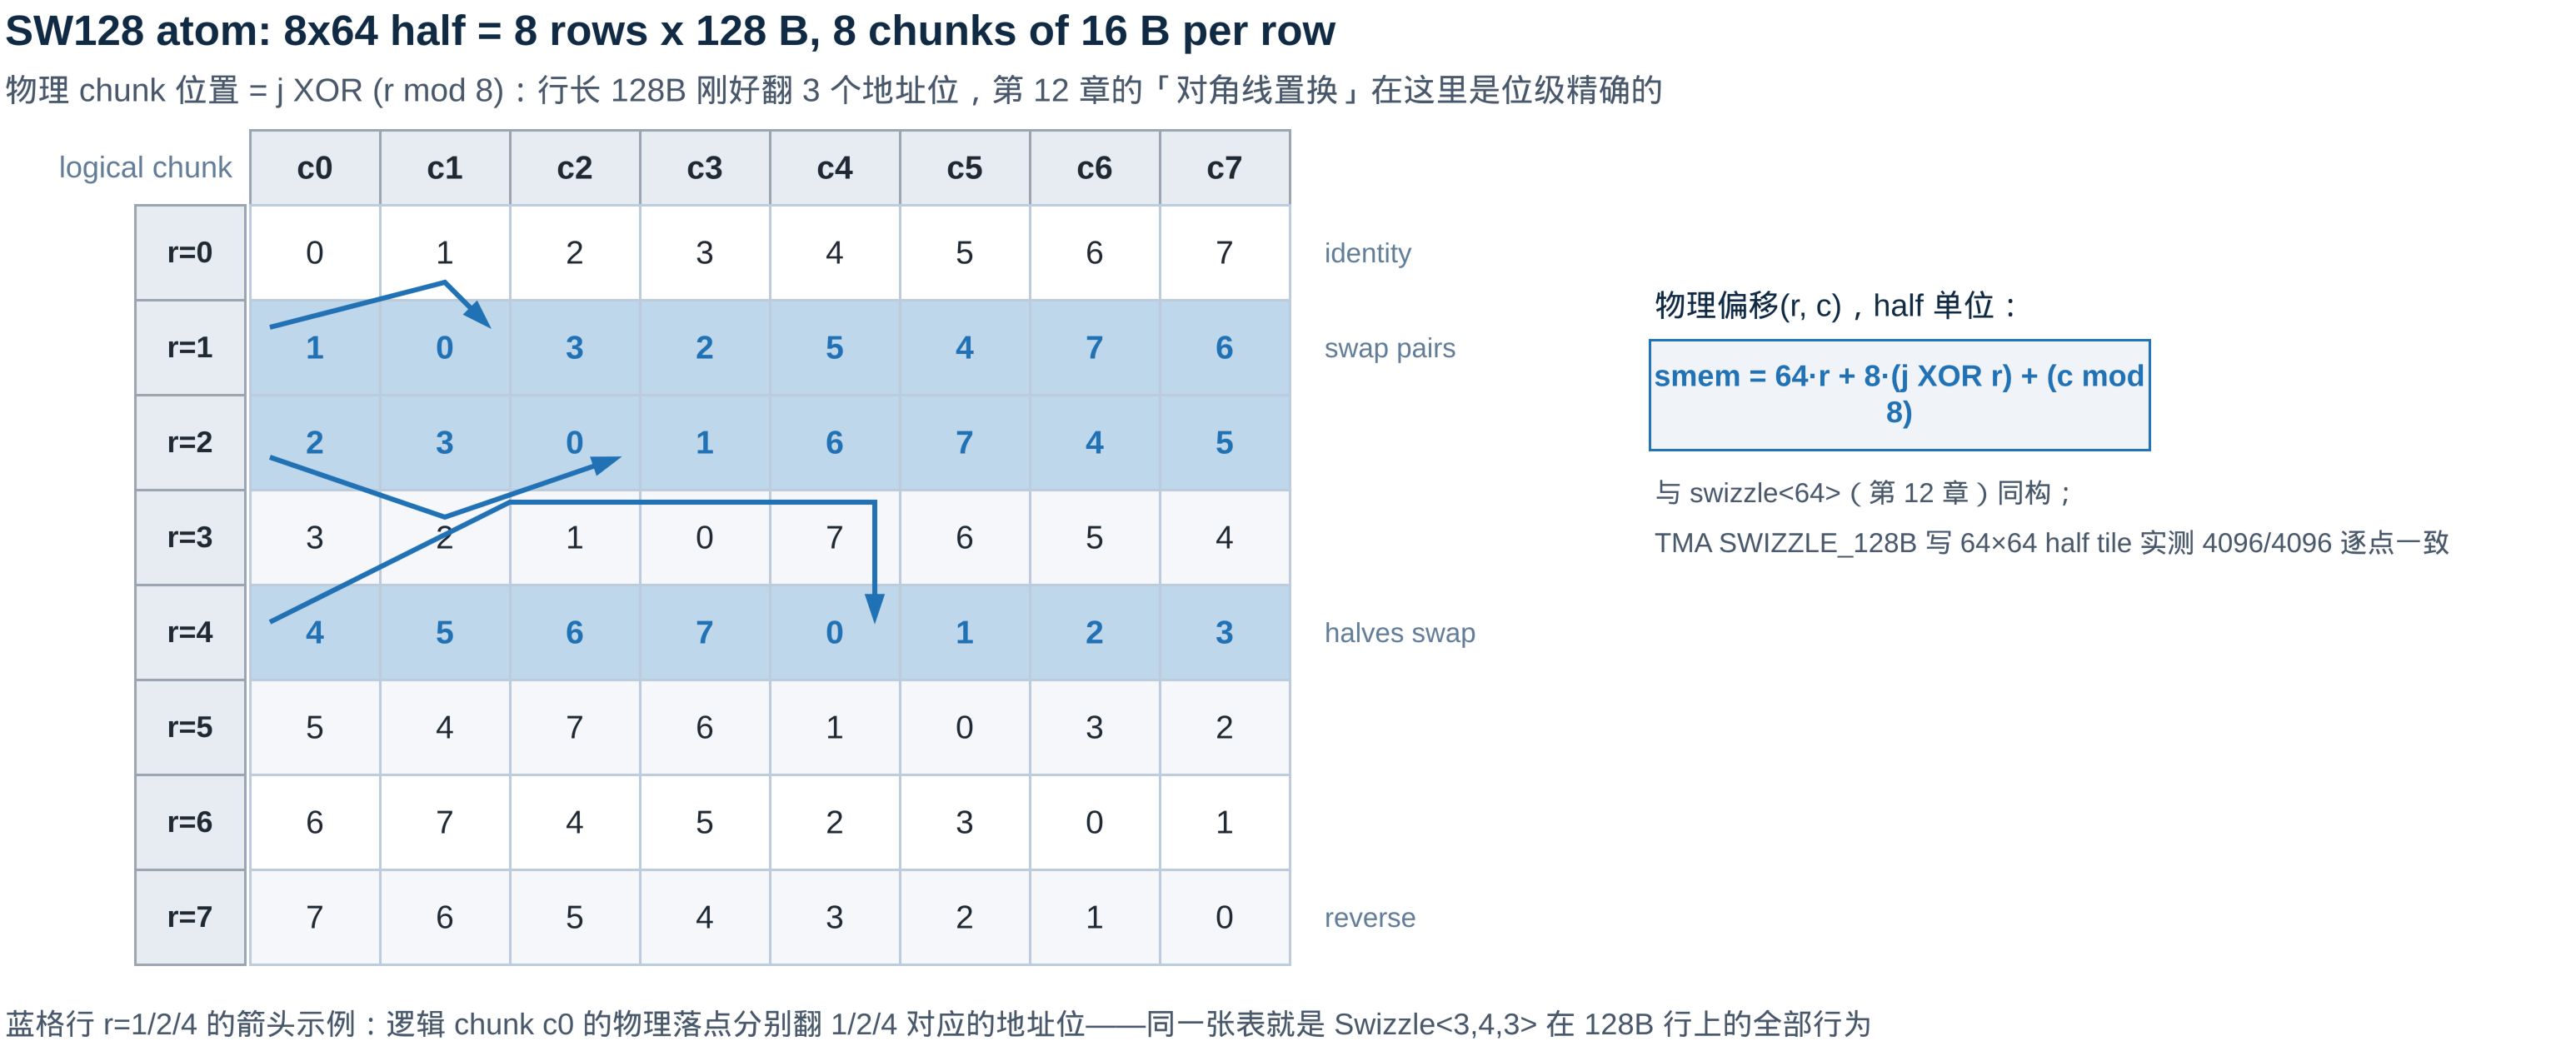
\includegraphics[width=0.9\textwidth]{figures/drawio/fig-23-1-sw128/fig-23-1.png}
\begin{tikzpicture}[font=\tiny, x=0.01525cm, y=-0.01525cm]
  \node[anchor=west, font=\footnotesize\bfseries] at (30,26)
    {SW128 atom: 8$\times$64 half $=$ 8 rows $\times$ 128 B, 8 chunks of 16 B per row};
  \node[anchor=west, font=\scriptsize] at (30,50)
    {物理 chunk 位置 $= j \oplus (r \bmod 8)$：行长 128\,B 刚好翻 3 个地址位，
     第~\ref{ch:12}~章的\textbf{对角线置换}在这里是位级精确的};
  \node[anchor=west, font=\tiny, text=gray!80] at (24,81) {logical chunk};
  \foreach \cc in {0,...,7}{
    \node[draw=gray!45, fill=gray!12, font=\tiny\bfseries, minimum width=0.79cm,
          minimum height=0.46cm, inner sep=0pt] at ({156+52*\cc},81) {c\cc};
  }
  \foreach \rr in {0,...,7}{
    \node[anchor=east, font=\tiny\bfseries, text=gray!80, minimum height=0.58cm]
      at (128,{115+38*\rr}) {r=\rr};
    \foreach \cc in {0,...,7}{
      \pgfmathtruncatemacro{\vv}{int(mod(\cc+\rr,2)) +
        2*int(mod(int(\cc/2)+int(\rr/2),2)) + 4*int(mod(int(\cc/4)+int(\rr/4),2))}
      \ifnum\rr=1
        \node[draw=gray!45, fill=tkFillBlue, text=tkBlue, minimum width=0.79cm,
              minimum height=0.58cm, inner sep=0pt] at ({156+52*\cc},{115+38*\rr}) {\vv};
      \else\ifnum\rr=2
        \node[draw=gray!45, fill=tkFillBlue, text=tkBlue, minimum width=0.79cm,
              minimum height=0.58cm, inner sep=0pt] at ({156+52*\cc},{115+38*\rr}) {\vv};
      \else\ifnum\rr=4
        \node[draw=gray!45, fill=tkFillBlue, text=tkBlue, minimum width=0.79cm,
              minimum height=0.58cm, inner sep=0pt] at ({156+52*\cc},{115+38*\rr}) {\vv};
      \else\ifnum\rr=3
        \node[draw=gray!45, fill=gray!6, minimum width=0.79cm, minimum height=0.58cm,
              inner sep=0pt] at ({156+52*\cc},{115+38*\rr}) {\vv};
      \else\ifnum\rr=5
        \node[draw=gray!45, fill=gray!6, minimum width=0.79cm, minimum height=0.58cm,
              inner sep=0pt] at ({156+52*\cc},{115+38*\rr}) {\vv};
      \else\ifnum\rr=7
        \node[draw=gray!45, fill=gray!6, minimum width=0.79cm, minimum height=0.58cm,
              inner sep=0pt] at ({156+52*\cc},{115+38*\rr}) {\vv};
      \else
        \node[draw=gray!45, fill=white, minimum width=0.79cm, minimum height=0.58cm,
              inner sep=0pt] at ({156+52*\cc},{115+38*\rr}) {\vv};
      \fi\fi\fi\fi\fi\fi
    }
  }
  \node[anchor=west, font=\tiny, text=gray!80] at (558,115) {identity};
  \node[anchor=west, font=\tiny, text=gray!80] at (558,153) {swap pairs};
  \node[anchor=west, font=\tiny, text=gray!80] at (558,267) {halves swap};
  \node[anchor=west, font=\tiny, text=gray!80] at (558,381) {reverse};
  \draw[-{Stealth[length=1.8mm]}, tkBlue, very thick] (138,142) -- (222,142);
  \draw[-{Stealth[length=1.8mm]}, tkBlue, very thick] (138,180) -- (274,180);
  \draw[-{Stealth[length=1.8mm]}, tkBlue, very thick] (138,256) -- (376,256);
  \node[anchor=west, font=\tiny, text=gray!80] at (690,136)
    {物理偏移$(r, c)$，half 单位：};
  \node[anchor=west, draw=tkBlue, fill=tkFillBlue, text=tkBlue, font=\tiny,
        inner sep=3pt] at (690,172)
    {smem $= 64r + 8(j \oplus r) + (c \bmod 8)$};
  \node[anchor=west, font=\tiny] at (690,211)
    {与 \texttt{swizzle<64>}（第~\ref{ch:12}~章）同构；};
  \node[anchor=west, font=\tiny] at (690,231)
    {TMA \texttt{SWIZZLE\_128B} 写 $64\times64$ half tile 实测 $4096/4096$ 逐点一致};
  \node[anchor=west, font=\tiny] at (30,424)
    {蓝格行 $r=1/2/4$ 的箭头示例：逻辑 chunk $c_0$ 的物理落点分别翻 $1/2/4$
     对应的地址位——同一张表就是 \texttt{Swizzle<3,4,3>} 在 128\,B 行上的全部行为};
\end{tikzpicture}
\caption{SW128 原子的物理排布：16\,B 块的列号 XOR 行号。横轴为 8 个
逻辑 chunk（$c_0$--$c_7$），纵轴 8 行，格内为该行接受置换后的物理
chunk 下标；蓝底行 $r=1/2/4$ 给出 chunk $c_0$ 落点翻转 $1/2/4$ 地址位的
示例。物理偏移 $=64r+8\cdot(j\oplus r)+(c\bmod 8)$（half 单位）——与
\texttt{swizzle<64>}（第~\ref{ch:12}~章）同构。}
\label{fig:23-1}
\end{figure}

\begin{figure}[htbp]
\centering
% was: 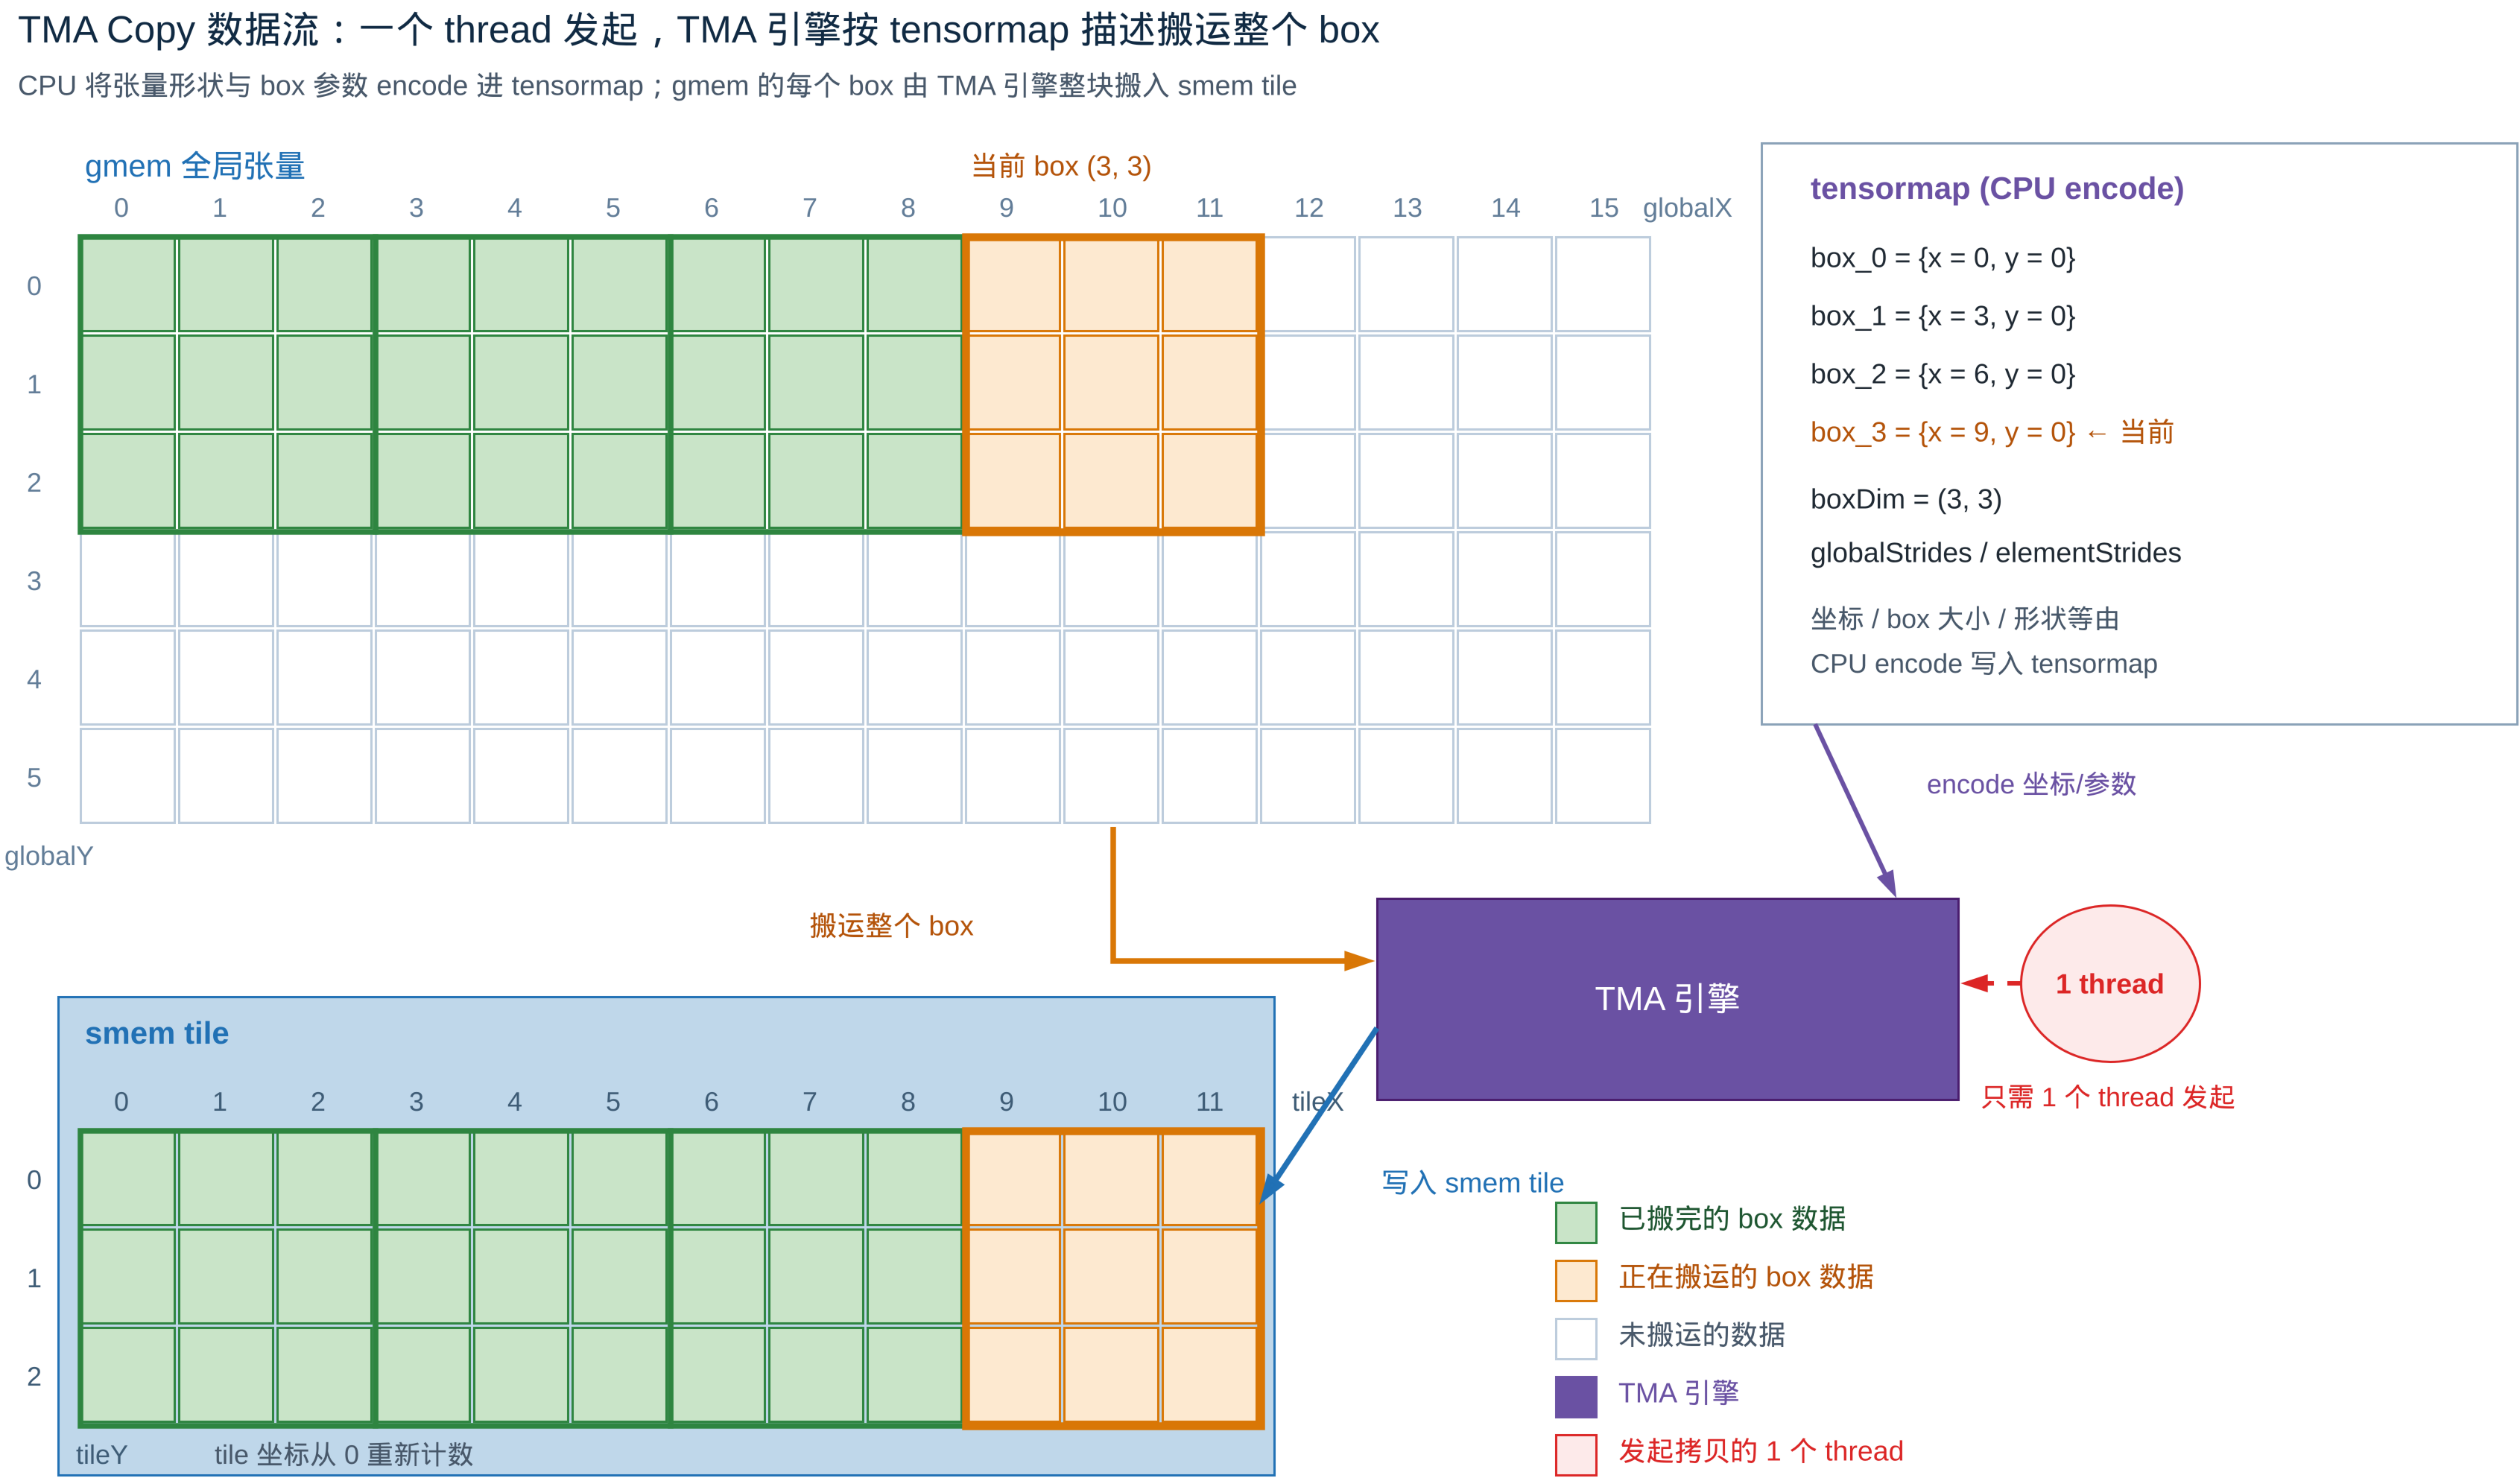
\includegraphics[width=0.95\textwidth]{figures/drawio/fig-23-2-tma-copy-flow/fig-23-2.png}
\begin{tikzpicture}[font=\tiny, x=0.015cm, y=-0.015cm]
  \node[anchor=west, font=\footnotesize\bfseries] at (30,23)
    {TMA Copy 数据流：一个 thread 发起，TMA 引擎按 tensormap 描述搬运整个 box};
  \node[anchor=west, font=\tiny] at (30,48)
    {CPU 将张量形状与 box 参数 encode 进 tensormap；gmem 的每个 box 由 TMA
     引擎整块搬入 smem tile};
  \node[anchor=west, font=\scriptsize, text=tkBlue] at (60,84) {gmem 全局张量};
  \node[anchor=west, font=\tiny, text=tkOrange!80!black] at (456,84)
    {当前 box $(3, 3)$};
  \foreach \cc in {0,...,15}{
    \node[font=\tiny, text=gray!80] at ({82+44*\cc},103) {\cc};
  }
  \foreach \rr in {0,...,5}{
    \node[anchor=east, font=\tiny, text=gray!80] at (52,{138+44*\rr}) {\rr};
    \foreach \cc in {0,...,15}{
      \ifnum\rr<3
        \ifnum\cc<9
          \node[draw=gray!40, fill=tkFillGreen, minimum width=0.63cm, minimum height=0.63cm,
                inner sep=0pt] at ({81+44*\cc},{137+44*\rr}) {};
        \else\ifnum\cc<12
          \node[draw=gray!40, fill=tkFillOrange, minimum width=0.63cm, minimum height=0.63cm,
                inner sep=0pt] at ({81+44*\cc},{137+44*\rr}) {};
        \else
          \node[draw=gray!40, fill=white, minimum width=0.63cm, minimum height=0.63cm,
                inner sep=0pt] at ({81+44*\cc},{137+44*\rr}) {};
        \fi\fi
      \else
        \node[draw=gray!40, fill=white, minimum width=0.63cm, minimum height=0.63cm,
              inner sep=0pt] at ({81+44*\cc},{137+44*\rr}) {};
      \fi
    }
  }
  \draw[tkGreen, very thick] (60,116) rectangle (192,248);
  \draw[tkGreen, very thick] (192,116) rectangle (324,248);
  \draw[tkGreen, very thick] (324,116) rectangle (456,248);
  \draw[tkOrange, very thick] (456,116) rectangle (588,248);
  \node[anchor=west, font=\tiny, text=gray!80] at (746,103) {globalX};
  \node[anchor=west, font=\tiny, text=gray!80] at (24,393) {globalY};
  \node[draw=gray!60, fill=white, minimum width=5.07cm, minimum height=3.9cm,
        inner sep=0pt] at (981,204) {};
  \node[anchor=west, font=\scriptsize, text=tkPurple] at (832,94)
    {tensormap (CPU encode)};
  \foreach \k/\t in {0/{box\_0 $= \{x = 0, y = 0\}$},
                     1/{box\_1 $= \{x = 3, y = 0\}$},
                     2/{box\_2 $= \{x = 6, y = 0\}$}}{
    \node[anchor=west, font=\tiny] at (832,{125+26*\k}) {\t};
  }
  \node[anchor=west, font=\tiny, text=tkOrange!80!black] at (832,203)
    {box\_3 $= \{x = 9, y = 0\}$ $\leftarrow$ 当前};
  \node[anchor=west, font=\tiny] at (832,233) {boxDim $= (3, 3)$};
  \node[anchor=west, font=\tiny] at (832,257) {globalStrides / elementStrides};
  \node[anchor=west, font=\tiny, text=gray!90] at (832,287)
    {坐标 / box 大小 / 形状等由};
  \node[anchor=west, font=\tiny, text=gray!90] at (832,307) {CPU encode 写入 tensormap};
  \node[draw=tkPurple, fill=tkPurple, text=white, font=\scriptsize\bfseries,
        minimum width=3.9cm, minimum height=1.35cm, inner sep=0pt] at (770,457)
    {TMA 引擎};
  \node[draw=tkRed, fill=tkFillRed, text=tkRed, font=\tiny\bfseries,
        minimum width=1.2cm, minimum height=1.05cm, inner sep=0pt] at (968,450)
    {1 thread};
  \node[anchor=west, font=\tiny, text=tkRed] at (908,501) {只需 1 个 thread 发起};
  \node[draw=tkBlue, fill=tkFillBlue, minimum width=8.16cm, minimum height=3.21cm,
        inner sep=0pt] at (322,563) {};
  \node[anchor=west, font=\scriptsize, text=tkBlue] at (60,472) {smem tile};
  \foreach \rr in {0,...,2}{
    \node[anchor=east, font=\tiny, text=gray!90] at (52,{538+44*\rr}) {\rr};
    \foreach \cc in {0,...,11}{
      \ifnum\cc<9
        \node[draw=gray!40, fill=tkFillGreen, minimum width=0.63cm, minimum height=0.63cm,
              inner sep=0pt] at ({81+44*\cc},{537+44*\rr}) {};
      \else
        \node[draw=gray!40, fill=tkFillOrange, minimum width=0.63cm, minimum height=0.63cm,
              inner sep=0pt] at ({81+44*\cc},{537+44*\rr}) {};
      \fi
    }
  }
  \draw[tkGreen, very thick] (60,516) rectangle (192,648);
  \draw[tkGreen, very thick] (192,516) rectangle (324,648);
  \draw[tkGreen, very thick] (324,516) rectangle (456,648);
  \draw[tkOrange, very thick] (456,516) rectangle (588,648);
  \foreach \cc in {0,...,11}{
    \node[font=\tiny, text=gray!90] at ({82+44*\cc},503) {\cc};
  }
  \node[anchor=west, font=\tiny, text=gray!90] at (592,503) {tileX};
  \node[anchor=west, font=\tiny, text=gray!90] at (56,661) {tileY};
  \node[anchor=west, font=\tiny] at (118,661) {tile 坐标从 0 重新计数};
  \draw[-{Stealth[length=2mm]}, tkOrange, very thick] (522,380) -- (522,440) -- (636,440);
  \node[anchor=west, font=\tiny, text=tkOrange!80!black] at (384,424) {搬运整个 box};
  \draw[-{Stealth[length=2mm]}, tkPurple, thick] (836,334) -- (872,409);
  \node[anchor=west, font=\tiny, text=tkPurple] at (884,361) {encode 坐标/参数};
  \draw[-{Stealth[length=2mm]}, tkBlue, very thick] (652,502) -- (588,546);
  \node[anchor=west, font=\tiny, text=tkBlue] at (640,539) {写入 smem tile};
  \draw[-{Stealth[length=2mm]}, tkRed, dashed, thick] (926,450) -- (904,450);
  \foreach \k/\t in {0/{已搬完的 box 数据}, 1/{正在搬运的 box 数据},
                     2/{未搬运的数据}, 3/{TMA 引擎}, 4/{发起拷贝的 1 个 thread}}{
    \ifnum\k=0
      \node[draw=tkGreen!60, fill=tkFillGreen, minimum width=0.27cm, minimum height=0.27cm,
            inner sep=0pt] at (729,{557+26*\k}) {};
    \else\ifnum\k=1
      \node[draw=tkOrange!70, fill=tkFillOrange, minimum width=0.27cm, minimum height=0.27cm,
            inner sep=0pt] at (729,{557+26*\k}) {};
    \else\ifnum\k=2
      \node[draw=gray!40, fill=white, minimum width=0.27cm, minimum height=0.27cm,
            inner sep=0pt] at (729,{557+26*\k}) {};
    \else\ifnum\k=3
      \node[draw=tkPurple, fill=tkPurple, minimum width=0.27cm, minimum height=0.27cm,
            inner sep=0pt] at (729,{557+26*\k}) {};
    \else
      \node[draw=tkRed, fill=tkFillRed, minimum width=0.27cm, minimum height=0.27cm,
            inner sep=0pt] at (729,{557+26*\k}) {};
    \fi\fi\fi\fi
    \node[anchor=west, font=\tiny] at (746,{555+26*\k}) {\t};
  }
\end{tikzpicture}
\caption{TMA copy 数据流：全局张量按 $3\times3$ box 切分（绿=已搬完、橙=搬运中），各 box 起始坐标与张量描述由 CPU encode 进 tensormap，TMA 引擎据此定位整块搬运。发起与搬运分离——单线程发起拷贝指令，box 内全部元素由 TMA 引擎异步搬入 smem；数据落地后改用 tile 局部坐标，与全局坐标脱钩。重建自 @竹熙佳处《写给大家看的 CuTe 教程：TMA Copy》。}
\label{fig:23-2}
\end{figure}

\section{性能分析}

本章没有为 CuTe swizzle 单独建 bench（Phase~7c 的数据由 \texttt{bench/bench\_leetcuda.cu}
的 \texttt{--bench} 统一采集；端到端性能对照见第~\ref{ch:14}、\ref{ch:24}~章）。
这里只给三条可核验的定量结论：

\textbf{(1) bank conflict 的消除是块级的。} 一个 16 B chunk 占 4 个
bank（128 B $=$ 32 个 4 B bank）。式~\eqref{eq:23-chunk} 保证同一列块
（固定 $j$）在 8 行里落到 8 个互不相同的物理 chunk，即 8 个 4-bank
组，这正好是 \texttt{ldmatrix}（每线程取 16 B）所需要的性质。第
\ref{sec:23-minitest}~节的 case C 把它写成固定 chunk、行扫描得 8 个
不同值，case F 则验证 $8\times32$ 原子的退化形态
（\texttt{chunk'} $=$ \texttt{chunk} $\oplus$ $(\text{row}\gg1)$，
XOR 值只有 $\{0,8,16,24\}$ 四种，相邻两行共享图样，8 行一周期）。

\textbf{(2) swizzle 不需要独立的数据重排指令。} 软件
\texttt{ldmatrix} 路径把 XOR 折叠进地址表达式，SASS 里可能多出一条
\texttt{LOP3} 或少量整数指令；TMA 路径则由 descriptor 让硬件完成相应模式。
因此应说“没有额外的数据搬运指令”，而不是“零条额外指令”。

\textbf{(3) TMA 的收益不在拷贝更快，而在同步与数据管理更简单。} 生产者
只有 1 个线程发指令（式~\eqref{eq:23-tx} 的字节数由硬件事务计数保证），
256 个线程不再参与 G$\to$S 的地址计算，也不再需要
\texttt{\_\allowbreak{}\_\allowbreak{}syncthreads}，hgemm.cuh~L1990--2012 的注释把这一点总结为
\textbf{barrier $+$ proxy fence 取代了 CTA 级同步}。对本章而言，快是
次要的；谁算地址、谁保证一致这两个问题的答案变得唯一，
才是 TMA 对 kernel 工程的主要贡献。

\begin{equation}
\label{eq:23-tx}
N_{\text{tx}} = (B_M\!\cdot\!B_K + B_N\!\cdot\!B_K)\times
\texttt{sizeof\allowbreak{}(half)} = (128\!\cdot\!64+128\!\cdot\!64)\times2 = 32768\ \text{B}.
\end{equation}

\section{常见坑}

\begin{enumerate}[leftmargin=2.2em]
\item \textbf{拿复合布局当偏移公式。} 带 swizzle 的
\texttt{Composed\allowbreak{}Layout} 求值是位置无关的，TMA 硬件是位置相关的：
同一个逻辑坐标在两个语义下可以指向不同物理地址。要么全用布局
（\texttt{make\_tensor}/\texttt{Tensor}），要么全用公式（第~\ref{ch:12}~章的
\texttt{swizzle<>}），混用必错。
\item \textbf{基址对齐不够。} 本章经典 TMA 三档的 smem 基址要求分别为：
32\,B swizzle 对齐 256\,B，64\,B 对齐 512\,B，128\,B 对齐 1024\,B。
不能把 WGMMA descriptor 的对齐要求套到 TMA；\texttt{ldmatrix} 本身
也没有 1024\,B 这一硬件对齐规则，它只消费软件算出的 lane 地址。
\item \textbf{把 $M$ 当成元素粒度。} $2^M$ 是\emph{基本块}的字节数
（16\,B $=2^4$），不是元素个数；fp32 里它等于 4 个元素，fp16 里等于
8 个元素。经典三档使用 $M=4$，但 128\,B 模式还有受版本和架构约束的
$M=5/6$ 原子粒度变体，不能泛称 descriptor 只接受 $M=4$。
\item \textbf{\texttt{tile\_\allowbreak{}to\_\allowbreak{}shape} 不整除。} $8\times64$ 原子铺
$B_K=32$ 会直接断言失败；要么换原子，要么改 tile 形状。
\item \textbf{把 \texttt{k\_step} 加在 swizzle 外部。} 只要 slice 宽度
不是 swizzle 周期的整数倍，偏移就必须放进 swizzle 内部
（hgemm.cuh~L2021--2034 的注释），否则某些 $k_{\text{step}}$ 的
chunk 会跨 slice 交叉。
\item \textbf{预期 swizzle 能消除所有 bank conflict。} 它保证的是
\textbf{同一个 16 B 块列在 8 行内落到 8 个不同块}；跨 32 行、或以
4 B 为粒度的模式（例如标量表查）它不保证。强度由 $B$ 与行宽共同决定：
hgemm 路径的 $8\times32$ 原子实际强度只有 2 bit（4 个 XOR 图样，
相邻两行共享图样、8 行一周期，4.1 节实践须知）。
\item \textbf{忘记 swizzle 是地址函数。} 想让按 (\texttt{row,col}) 求值
的布局与按 flat 偏移求值的公式一致，前提是行宽恰好等于
$2^{M+S}$ 字节。行宽不匹配时（例如 $B_K$ 取 48），两者不等。
\end{enumerate}

\section{面试要点速查}

\textbf{Q1：\texttt{Swizzle\allowbreak{}<B,\allowbreak{}M,\allowbreak{}S>} 的三个参数各是什么？}
$M$：被保留的连续低位位数（基本块宽 $2^M$ 字节）；$B$：XOR 掩码位数，
同时决定 TMA 模式名（32/64/128\,B $\leftrightarrow$ 1/2/3）。
$S$：\texttt{YYY} 相对 \texttt{ZZZ} 的位移；仅当行宽恰好为 $2^{M+S}$
字节时（三档中只有 SW128 满足，见 Q2）才等价于一行 $2^{M+S}$ 字节，
工程上恒取 3。约束 $|S|\ge B$。

\textbf{Q2：为什么 $S$ 恒为 3？} 三档的 XOR 源字段固定取自 bit~7
（128\,B 粒度）、目标字段固定取自 bit~4（16\,B 块），两者相距 3 位，
故字节口径下 $S$ 恒为 3、$M$ 恒为 4（与 dtype 无关）；档间只改 $B$
（1/2/3）与 box 内维（行宽 32/64/128\,B）。fp16 元素口径下 $M=3$
（hgemm 自用的 \texttt{Swizzle\allowbreak{}<3,\allowbreak{}3,\allowbreak{}3>} 即此口径）。

\textbf{Q3：为什么不直接写成列块 XOR 行号，还要用位运算？}
因为 TMA 与 WGMMA descriptor 用字节地址上的位域模式描述硬件行为；
列块 XOR 行号只有在行宽 $=2^{M+S}$ 时才与位公式等价
（式~\eqref{eq:23-chunk}）。\texttt{ldmatrix} 不执行 descriptor swizzle，
它只是接收软件已经算好的 lane 地址，因此软件也必须用同一套位公式。

\textbf{Q4：\texttt{composition} 的求值顺序？} 先算基础布局得偏移，
Swizzle 再作用其上：$R(c)=\text{Swizzle}(\text{Layout}(c))$。
Swizzle 不参与坐标分解。

\textbf{Q5：TMA swizzle 与手写 swizzle 的冲突点在哪？} 在相位。
TMA 硬件按绝对地址和 descriptor 模式算 phase，软件按相对偏移算；基址
必须满足所选模式的对齐要求：经典 32/64/128\,B 三档分别为
256/512/1024\,B。WGMMA 有 \texttt{base\_offset} 字段可以补偿；
\texttt{ldmatrix} 没有这个字段，只能由软件地址计算保证一致。

\textbf{Q6：给定 $B_K$ 与 fp16，怎么判断该用哪种 swizzle？} 先算行宽
$B_K\times2$ 字节；可选行宽 32/64/128\,B，要求 $B_K\times2\ge$
模式行宽且 $16$\,B 块宽整除行宽。$B_K=64$ 时行宽 128\,B
$\Rightarrow$ \texttt{Swizzle\allowbreak{}<3,\allowbreak{}4,\allowbreak{}3>}（字节）或 \texttt{Swizzle\allowbreak{}<3,\allowbreak{}3,\allowbreak{}3>}
（元素）；$B_K=32$ 时行宽 64\,B，只能退到 64\,B 或更弱的模式。

\section{最小测试与动手实验}\label{sec:23-minitest}

\texttt{book/\allowbreak{}tests/\allowbreak{}ch23\_\allowbreak{}swizzle\_\allowbreak{}tma.cu} 是一个主机侧断言程序
（需要 \texttt{NOTES\_\allowbreak{}V2\_\allowbreak{}ENABLE\_\allowbreak{}CUTE}），它把本章的公式逐条与 CuTe 的
布局求值结果对照，不启动任何 kernel。七个 case：

\begin{enumerate}[leftmargin=2.2em]
\item \textbf{case A}：\texttt{Swizzle\allowbreak{}<3,\allowbreak{}3,\allowbreak{}3>} 的位级公式：对
$[0,1024)$ 内每个字节偏移验证 $\text{apply}(\text{off})=\text{off}\oplus
((\text{off}\wedge(\texttt{0b111}\ll6))\gg3)$，并核对
\texttt{yyy\_msk}/\texttt{zzz\_msk} 常量、统计 $8$ 个 \texttt{YYY} 值与
$8$ 个 chunk 各被覆盖 $128$ 次；
\item \textbf{case B}：对合性 $\text{apply}(\text{apply}(x))=x$ 与
$[0,512)$ 上的双射，再用自定义 base layout
$\texttt{\allowbreak{}(8,\allowbreak{}8):\allowbreak{}(64,\allowbreak{}8)}$（64\,B 行、8\,B 块）验证
$R(r,c)=64r+8\cdot(c\oplus r)$，并检查固定块列扫 $8$ 行得到 $8$ 个
不同物理块、$8$ 个不同 bank；
\item \textbf{case C}：把字节空间的 \texttt{Swizzle\allowbreak{}<3,\allowbreak{}4,\allowbreak{}3>}（即
\texttt{make\_tensor} 后指针路径的位置相关语义）作用在
\texttt{GMMA::\allowbreak{}Layout\_\allowbreak{}K\_\allowbreak{}SW128\_\allowbreak{}Atom\allowbreak{}<half>} 的 $8\times64$ 域上，
$512$ 个坐标全部满足式~\eqref{eq:23-chunk}；
\item \textbf{case D}：\texttt{composition} 语义
$R(c)=\text{Swizzle}(\text{Base}(c))$，两种 base layout 各遍历全
domain（$256+256$ 个坐标）；
\item \textbf{case E}：硬件对照：sm\_120a 实测的 TMA
\texttt{SWIZZLE\_\allowbreak{}128\allowbreak{}B} $8\times8$ chunk 掩码表（$64$ 槽）与
\texttt{Swizzle\allowbreak{}<3,\allowbreak{}4,\allowbreak{}3>} 逐槽比较，再由该表导出 $4096$ 点排布逐点比较；
同时统计 \texttt{tile\_\allowbreak{}to\_\allowbreak{}shape} 分块布局\emph{裸求值}的命中数
（$1024/4096$），用于说明把字节口径 swizzle 直接套在元素偏移上的
单位错配（补上 $\times2$ recast 后应 $4096/4096$）；
\item \textbf{case F}：$8\times32$ 原子的退化形态（4.1 节实践须知）：
验证 $\text{chunk}'=\text{chunk}\oplus(\text{row}\gg1)$，XOR 值集合为
$\{0,8,16,24\}$、每个值覆盖 $2$ 行（$=64$ 个坐标）；
\item \textbf{case G}：TMA 编译级核对：\texttt{Tma\allowbreak{}Descriptor}
$=$ \texttt{CUtensorMap} 且尺寸为 $128$\,B、三档掩码常量、SW128 atom 的
\texttt{layout\_a()}/\texttt{layout\_b()} 类型与其 \texttt{shape}/
\texttt{stride}/cosize，以及在 host 侧用 \texttt{make\_\allowbreak{}tma\_\allowbreak{}copy}
真正构造出一个 descriptor 并核对 (gmem 张量, CTA tile) 的
size/stride 推导。
\end{enumerate}

编译与运行：

\begin{lstlisting}[style=console]
  cd book/tests
  ./build_tests.sh --arch sm_120a --ch ch23
\end{lstlisting}

预期输出（$2026$-$09$-$11$ 于 RTX PRO 5000 / sm\_120a 实机执行，全文）：

\begin{lstlisting}[style=console]
== ch23 CuTe swizzle / TMA (host-side assertions) ==
PASS case A Swizzle<3,3,3> bit formula: mismatches=0 (1044 checks)
PASS case B involution + bijection + base layout: mismatches=0 (1105 checks)
PASS case C byte-space Sw<3,4,3> == chunk XOR row: mismatches=0 (576 checks)
PASS case D composition R(c) == Swizzle(Base(c)): mismatches=0 (512 checks)
      (E) measured table mismatches=0
      (E) 4096-point mismatches=0, tiled formula 1024/4096
PASS case E hardware SWIZZLE_128B cross-check: mismatches=0 (3 checks)
PASS case F hgemm 8x32 atom effective swizzle: mismatches=0 (262 checks)
PASS case G TMA compile-level (descriptor): mismatches=0 (15 checks)
ALL OK
\end{lstlisting}
（\texttt{tiled formula 1024/4096} 一行是裸求值（字节口径 swizzle 直接
作用在元素偏移上）的口径错配结果，补上 $\times2$ recast 后为
$4096/4096$。\texttt{build\_\allowbreak{}tests.\allowbreak{}sh} 在该输出之后还会再打印一次
\texttt{ALL OK} 作为汇总，退出码 $0$。）

动手实验（可选）：把 case F 里的 \texttt{Swizzle\allowbreak{}<3,\allowbreak{}3,\allowbreak{}3>} 换成
\texttt{Swizzle\allowbreak{}<3,\allowbreak{}4,\allowbreak{}3>}（相当于把 $8\times32$ 原子按 128\,B 行宽去解释），
重跑并打印 XOR 值集合。两次结果的差异正是 4.1/3.3 节实践须知要读者亲手
复现的那一步：\textbf{同一个 \texttt{Swizzle} 类型在不同 base layout 下的
物理效果不同，参数必须与行宽一起读}。

\section*{延伸阅读}

\begin{itemize}[leftmargin=1.6em]
\item @reed，\emph{cute 之 Swizzle}（ch12/23 主参考）：
\url{https://zhuanlan.zhihu.com/p/671419093}
\item @reed，\emph{cute 之 TMA Descriptor 编码与隐藏的第 21bit}
（descriptor 字段与 swizzle 模式编码）：
\url{https://zhuanlan.zhihu.com/p/2037200219700449995}
\item @竹熙佳处，\emph{CuTe 教程：TMA Copy}（\texttt{make\_\allowbreak{}tma\_\allowbreak{}copy}
的用法与边界）：
\url{https://zhuanlan.zhihu.com/p/2003198909405763007}
\item @weishengying，\emph{cute swizzle}（可运行的最小例子）：
\url{https://zhuanlan.zhihu.com/p/706796240}
\item @Anonymous，\emph{GEMM 细节分析（三）：Swizzle<B,M,S> 参数取值}
（三个档位的参数对照）：\url{https://zhuanlan.zhihu.com/p/713713957}
\end{itemize}

% ch24-cute-hgemm.tex — CuTe 应用（一）：HGEMM（RFC-F，2026-09-11）
% \url 由 book.tex 的 hyperref 提供；单章独立编译时降级为可断行的 \ttfamily
% （逐字符插入 \allowbreak，避免长 URL 造成 Overfull \hbox）
\makeatletter
\providecommand{\urlchbrk}[1]{\@tfor\next:=#1\do{\next\allowbreak}}
\makeatother
\providecommand{\url}[1]{{\ttfamily\urlchbrk{#1}}}
\chapter{CuTe 应用（一）：HGEMM}\label{ch:24}

\section{本章导读}

第~\ref{ch:11}、\ref{ch:12}~章用两条不同的路把同一个 HGEMM 写了两遍：一条是
手写 MMA PTX $+$ 手算 smem 地址的 Phase~7b，另一条是手写 XOR swizzle $+$
寄存器双缓冲的 Phase~7b-3。Phase~7b-3 跑到了 122.9\,TFLOPS
（2048$\times$16384），Phase~7b 为 76.55\,TFLOPS（1024$^3$），但代价是同一组
形状与步长的事实被反复重写：\texttt{ldmatrix} 的 lane 映射、swizzle 的
XOR 掩码、epilogue 的 \texttt{\_\_shfl\_sync} 编排，每一处都要人工保证与其余
四处的地址算术一致。本章把同一个 kernel 交给 CuTe 重写一遍，用的是 Phase~7c 的
\texttt{hgemm\_\allowbreak{}mma\_\allowbreak{}stages\_\allowbreak{}tn\_\allowbreak{}cute}，并在最后用一张对照表
（图~\ref{fig:24-1}）把两条路逐项摆开。

\textbf{前置章节}：第~\ref{ch:11}~章（\texttt{mma.\allowbreak{}sync.\allowbreak{}m16n8k16} 与
\texttt{ldmatrix}）、第~\ref{ch:12}~章（XOR swizzle 与寄存器双缓冲）、
第~\ref{ch:20}--\ref{ch:23}~章（Layout 代数 / Tensor 与 TiledCopy / TiledMMA /
Swizzle 与 TMA）。本章是 Part~IV 的第一章\textbf{应用篇}，只用到前四章已经介绍过的
四个抽象：\texttt{Layout}、\texttt{Tensor}、\texttt{TiledCopy}、
\texttt{TiledMMA}。

\textbf{阅读路线}：本章沿 @reed 的 CuTe GEMM 三部曲《cute 之 简单 GEMM
实现》《cute 之 GEMM 流水线》《cute 之 高效 GEMM 实现》（链接见文末
\textbf{延伸阅读}）的叙述顺序，按先跑通 $\to$ 再重叠 $\to$ 后提速三步渐进展开。
每一步开头先说明上一版留下了什么问题，再给出这一版的代码，以及读者必须
自己守住的约束。凡是源码注释与实现不一致、或表述容易被误读的地方，不再集中
堆在章末的勘误节，而是就地写成\textbf{实践须知}：这类提醒出现在使用现场比
事后查表更有用。

\textbf{源码区间}：hgemm.cuh~L718--1427：Phase~7c 头注释（L718--778）、
宏块 \texttt{NOTES\_\allowbreak{}V2\_\allowbreak{}ENABLE\_\allowbreak{}CUTE}（L779--1427）内的 kernel
\texttt{hgemm\_\allowbreak{}mma\_\allowbreak{}stages\_\allowbreak{}tn\_\allowbreak{}cute}（L821 起）与 launch wrapper
\texttt{launch\_\allowbreak{}hgemm\_\allowbreak{}mma\_\allowbreak{}stages\_\allowbreak{}tn\_\allowbreak{}cute}（L1216 起）。\textbf{编译宏}：
\texttt{NOTES\_\allowbreak{}V2\_\allowbreak{}ENABLE\_\allowbreak{}CUTE}（需要 CUTLASS 头文件；sm80 及以上均可编）。
\textbf{架构}：本章 kernel 只用 SM80 时代的 \texttt{cp.async} $+$
\texttt{mma.sync} $+$ \texttt{ldmatrix}，本机 sm\_120a 可实测。

配套最小测试 \texttt{book/\allowbreak{}tests/\allowbreak{}ch24\_\allowbreak{}hgemm\_\allowbreak{}cute.cu}：两组配置
（\texttt{k\allowbreak{}Acc\allowbreak{}F32=\allowbreak{}false}、$B_N=256$ 与 \texttt{k\allowbreak{}Acc\allowbreak{}F32=\allowbreak{}true}、$B_N=128$）对 CPU
fp64 参考做正确性判定；本章的实测数字全部来自该测试与 \texttt{ptxas -v}，
端到端性能对照见第~\ref{sec:ch24-perf}~节。

\section{问题与动机}

先把第~\ref{ch:11}、\ref{ch:12}~章的代码量摆出来（只统计代码行，去掉纯注释
与空行；统计口径见第~\ref{sec:24-minitest}~节）：

\begin{itemize}
  \item Phase~7b \texttt{hgemm\_\allowbreak{}mma\_\allowbreak{}stages\_\allowbreak{}tn}（hgemm.cuh~L129--397）：
        151 行；
  \item Phase~7b-3 \texttt{hgemm\_\allowbreak{}mma\_\allowbreak{}stages\_\allowbreak{}tn\_\allowbreak{}swizzle}
        （hgemm.cuh~L434--716）：235 行；
  \item Phase~7c \texttt{hgemm\_\allowbreak{}mma\_\allowbreak{}stages\_\allowbreak{}tn\_\allowbreak{}cute}
        （hgemm.cuh~L821--1196）：118 行，再加 launch wrapper
        （L1216--1427）86 行。
\end{itemize}

手写版与 CuTe 版的行数比并不悬殊（235 对 204），但代码的性质变了。
手写版里出现的是地址表达式与内联 PTX：

\begin{lstlisting}
int lane_smem_a_m = warp_m * (kMmaM * kValTileM) + i * kMmaM + lane_id % 16;
int lane_smem_a_k = k_step * kMmaK + (lane_id / 16) * 8;
uint32_t lane_smem_a_ptr = smem_a_base_ptr +
    (stage * BM * BK + lane_smem_a_m * BK +
     swizzle<64>(lane_smem_a_m, lane_smem_a_k)) * sizeof(half);
LDMATRIX_X4(RA[i][0], RA[i][1], RA[i][2], RA[i][3], lane_smem_a_ptr);
\end{lstlisting}

CuTe 版里出现的是声明与分区：

\begin{lstlisting}
auto sA = make_tensor(make_smem_ptr(Ashm), SmemLayoutA{});
auto tAsA = s2r_thr_copy_a.partition_S(sA);
auto tCrA_view = s2r_thr_copy_a.retile_D(tCrA);
cute::copy(s2r_tiled_copy_a, tAsA(_, _, k_step_next, ismem_read),
           tCrA_view(_, _, k_step_next));
\end{lstlisting}

前者把 \texttt{lane} 到 smem 地址的公式写死在 kernel 里，改一个 tile 尺寸就
要把公式推倒重来；后者把同一件事表达成两句声明：\texttt{sA} 的布局是
\texttt{SmemLayoutA}，\texttt{s2r\_\allowbreak{}thr\_\allowbreak{}copy\_\allowbreak{}a} 把 sA 按线程切分。
地址算术由编译器（类型系统）展开，这是第~\ref{ch:20}--\ref{ch:23}~章铺垫四章
换来的东西：把布局从代码里提出来，变成一等公民。

本章要回答三个问题：这 118 行的 kernel 本体做了什么？launch wrapper 的 86 行
类型实例化在配置什么？哪些东西 CuTe 替你做了，哪些仍要你自己做？第三个问题
决定这套工具的能力边界，也是图~\ref{fig:24-1} 要回答的。

正文按三步渐进展开，三步共用同一份源码事实，区别只在每一步放弃或引入什么。

\section{数学原理}

\subsection{问题定义：TN 约定与第一个 Tensor}

本章沿用第~\ref{ch:11}~章的 TN 约定：
$C[M,N] = A[M,K]\times B^{\mathsf T}[N,K]$，其中 $A$、$B^{\mathsf T}$ 都是
row-major（\texttt{A[m][k]}、\texttt{Bt[n][k]}）。写成求和形式：

\begin{equation}
  C_{m,n} \;=\; \sum_{k=0}^{K-1} A_{m,k}\, B_{n,k},
  \label{eq:24-tn}
\end{equation}

注意式~\eqref{eq:24-tn} 里 $B$ 的索引是 $(n,k)$，这就是 TN 的含义：MMA 指令
\texttt{mma.\allowbreak{}sync.\allowbreak{}aligned.\allowbreak{}m16n8k16.row.\allowbreak{}col} 要求 A 为 row-major、B 在 GEMM
语义下为 col-major，而 col-major 的 $B[K,N]$ 与 row-major 的
$B^{\mathsf T}[N,K]$ 是同一块内存。这是本章第一个坑：调用方必须自己把 $B$
转置后传入（最小测试里由 host 侧转置完成，见第~\ref{sec:24-minitest}~节）。

用 CuTe 的话说，TN 是一句关于步长的声明，而不是标志位：

\begin{lstlisting}
  Tensor A = make_tensor(make_gmem_ptr(Aptr), make_shape(m, k),
                         make_stride(k, Int<1>{}));  // A 是 (M,K)，K 连续
  Tensor B = make_tensor(make_gmem_ptr(Bptr), make_shape(n, k),
                         make_stride(k, Int<1>{}));  // Bt 是 (N,K)，K 连续
\end{lstlisting}

两行 \texttt{make\_tensor} 之后，后续所有分区与拷贝都在\textbf{$(shape,stride)$
就是布局}这条约定上工作：$K$ 维连续意味着按 $K$ 切出来的片天然适合做
\texttt{cp.async} 的宽拷贝，而 \texttt{Int<1>\{\}} 这个编译期常量会让
后面每一步的地址算术都在编译期折叠掉。

\subsection{Tile 金字塔：从 CTA tile 到 MMA atom}

一个 CTA 只负责 $C$ 的一小块，整张 $C$ 由网格铺满；$K$ 方向则切开累加
（sliced-K 模式，第~\ref{ch:09}~章）：设 CTA 级 tile 为
$B_M\times B_N\times B_K$，网格为
$\bigl(\lceil N/B_N\rceil,\lceil M/B_M\rceil\bigr)$。Phase~7c 的默认配置：

\begin{equation}
  B_M=128,\qquad
  B_N=\begin{cases}256, & \text{F16 累加}\\ 128, & \text{F32 累加}\end{cases},
  \qquad B_K=32,\qquad k_{\mathrm{stage}}=2 .
  \label{eq:24-tile}
\end{equation}

这三个数字构成一座三层金字塔：CTA tile $B_M\times B_N$（一次搬进来、一次算完）
$\supset$ 逻辑 MMA tile $32\times32\times16$（\texttt{TiledMMA} 一次展开多少条
指令，见下节）$\supset$ atom $16\times8\times16$（一条 \texttt{mma.sync}）。
CuTe 的层层 partition 就是在这座金字塔上做从塔基切到塔尖的坐标换算。三层之间
的尺寸关系见图~\ref{fig:24-tile-pyramid}。

\begin{figure}[H]
\centering
\begin{tikzpicture}[font=\tiny]
  \foreach \gr in {0,...,3}{
    \foreach \gc in {0,...,7}{
      \node[fill=gray!22, minimum width=0.5cm, minimum height=0.5cm, inner sep=0pt]
        at ({\gc*0.5+0.25},{-\gr*0.5-0.25}) {};
    }
  }
  \node[fill=tkOrange!30, draw=tkOrange!80!black, thin, minimum width=0.5cm, minimum height=0.5cm, inner sep=0pt]
    at (3.75,-0.75) {};
  \draw[thin] (0,0) grid[xstep=0.5cm, ystep=0.5cm] (4.0,-2.0);
  \draw[very thick] (0,0) rectangle (4.0,-2.0);
  \node[anchor=south, align=center, font=\scriptsize\bfseries, text width=4.0cm]
    at (2.0,0.12) {CTA tile\\ $B_M\times B_N=128\times256$};
  \node[anchor=north, align=center, text width=4.6cm] at (2.0,-2.1)
    {灰块 $=$ 一个 $32\times32$ MMA tile（$4\times8$ 个铺满整块）};
  \draw[->, very thick] (4.25,-0.75) -- (5.1,-0.75);
  \node[anchor=south] at (4.65,-0.72) {取 1 个};
  \begin{scope}[shift={(5.2,0)}]
    \foreach \wr in {0,...,1}{
      \foreach \wc in {0,...,1}{
        \pgfmathtruncatemacro{\wg}{2*\wr+\wc}
        \ifcase\wg
          \def\wcol{colorx6}%
        \or
          \def\wcol{colorx5}%
        \or
          \def\wcol{colorx4}%
        \else
          \def\wcol{colorx7}%
        \fi
        \node[fill=\wcol!40, minimum width=1.0cm, minimum height=1.0cm, inner sep=0pt]
          at ({\wc*1.0+0.5},{-\wr*1.0-0.5}) {w\wg};
      }
    }
    \draw[thin] (0,0) grid[xstep=1.0cm, ystep=1.0cm] (2.0,-2.0);
    \draw[very thick] (0,0) rectangle (2.0,-2.0);
    \node[anchor=south, align=center, font=\scriptsize\bfseries, text width=3.4cm]
      at (1.0,0.12) {逻辑 MMA tile\\ $32\times32\times16$};
    \node[anchor=north, align=center, text width=4.2cm] at (1.0,-2.1)
      {AtomLayout$(M,N,K)=(2,2,1)$：$2\times2$ 个 warp，\\ 每个 warp 覆盖
       $16\times16$（EURepeat$\times$atom）};
  \end{scope}
  \draw[->, very thick] (7.3,-0.5) -- (8.95,-0.5);
  \node[anchor=south] at (8.1,-0.47) {每 warp 内};
  \begin{scope}[shift={(9.0,-0.2)}]
    \foreach \arow in {0,...,15}{
      \foreach \acol in {0,...,7}{
        \node[fill=gray!18, minimum width=0.16cm, minimum height=0.16cm, inner sep=0pt]
          at ({\acol*0.16+0.08},{-\arow*0.16-0.08}) {};
      }
    }
    \draw[thin] (0,0) grid[xstep=0.16cm, ystep=0.16cm] (1.28,-2.56);
    \draw[very thick] (0,0) rectangle (1.28,-2.56);
    \node[anchor=north west, align=left, text width=3.8cm] at (1.45,-0.25)
      {$M$ 方向 $16$ 行（mode 0 向下）、$N$ 方向 $8$ 列（mode 1 向右）；
       每线程 $4$ 个 float 累加器（m16n8k16 的 C fragment）。};
  \end{scope}
  \node[anchor=south west, font=\scriptsize\bfseries] at (8.8,0.12)
    {atom $16\times8\times16$（一条 \texttt{mma.sync}）};
  \node[anchor=north west, align=left, text width=15.5cm] at (0,-3.1)
    {三层尺寸关系：$\texttt{kMmaPM}=\mathrm{AtomLayout}_M(2)\times16=32$、
     $\texttt{kMmaPN}=\mathrm{AtomLayout}_N(2)\times\mathrm{EURepeat}_N(2)
     \times8=32$、$\texttt{kMmaPK}=1\times16=16$；线程数 $=32$ lanes
     $\times$ $4$ warps $=128$；$n_{k\text{-step}}=B_K/\texttt{kMmaPK}=2$。
     CTA tile 一次搬进来、一次算完：smem
     $=128\cdot32\cdot2+256\cdot32\cdot2=24576$ half $=48$\,KiB
     （式~\eqref{eq:24-smem}）。$B_N=256$ 只在 F16 累加下成立，F32 累加时
     掉到 $128$——$128\times256/128=256$ 个 f32 逻辑累加值已超过每线程
     255 个寄存器的硬上限，尚未计其他临时量。};
\end{tikzpicture}
\caption{本章实际配置的三层 tile 金字塔（式~\eqref{eq:24-tile} 与
式~\eqref{eq:24-tile-mma}）：外层 CTA tile $128\times256$ 一次搬进 smem、
一次算完（F16 累加；F32 累加时 $B_N$ 降到 $128$）；中层逻辑 MMA tile
$32\times32\times16$ 被 AtomLayout$(2,2,1)$ 切成 $2\times2$ 个 warp（每个
warp 覆盖 $16\times16$，由 EURepeat$\times$atom 堆出）；内层 atom
$16\times8\times16$ 就是一条 \texttt{mma.sync}。}
\label{fig:24-tile-pyramid}
\end{figure}

$B_N$ 随累加精度切换是寄存器预算的算术结果：F32 累加器每个元素占
4 字节，寄存器压力翻倍。$128\times256$ 的 C tile 在 128 线程下是
$128\cdot256/128=256$ 个 f32 逻辑累加值，已经超过每线程 255 个 32-bit
寄存器的硬上限；再计入地址、流水与临时寄存器后必然溢出到 local memory。第~\ref{sec:24-step3b}~节把两种精度的寄存器占用摆开，并用
\texttt{ptxas -v} 的实测数字核对（口径讨论见第~\ref{sec:24-kaogu}~节）。
$B_K=32$ 与 $k_{\mathrm{stage}}=2$ 一起决定了 smem 占用：

\begin{equation}
  \underbrace{128\cdot32\cdot2}_{\text{A：}\allowbreak{}B_M B_K k_{\mathrm{stage}}}
  +\underbrace{256\cdot32\cdot2}_{\text{B：}\allowbreak{}B_N B_K k_{\mathrm{stage}}}
  = 24576\ \text{个 half} = 48\,\text{KiB},
  \label{eq:24-smem}
\end{equation}

这个 kernel 于是落在每 CTA 占 48\,KiB smem 这一档（本机 PRO~5000
（cc~12.0）实测每 SM smem 上限 102400\,B $=$ 100\,KiB，一个 48\,KiB 的 CTA
每 SM 至多驻留 2 个；占用率还要受寄存器与 block 数约束）。

\subsection{MMA atom 与 EURepeat}

一个 CTA tile 要想算完，先要回答两个问题：一条 \texttt{mma.sync} 能算多大
（\textbf{atom}），以及把多少条这样的指令铺在一个 warpgroup 上
（\textbf{EURepeat}）。atom 取 SM80 的 \texttt{m16n8k16}，A/B 均为 fp16、
累加器可选 fp16 或 fp32：

\begin{center}
\begin{tabular}{lll}
\toprule
项 & F16 累加 & F32 累加 \\
\midrule
PTX 形状 & \texttt{m16n8k16} & \texttt{m16n8k16} \\
CuTe atom & \texttt{SM80\_\allowbreak{}16x8x16\_\allowbreak{}F16\allowbreak{}F16\allowbreak{}F16\allowbreak{}F16\_\allowbreak{}TN}
           & \texttt{SM80\_\allowbreak{}16x8x16\_\allowbreak{}F32\allowbreak{}F16\allowbreak{}F16\allowbreak{}F32\_\allowbreak{}TN} \\
C 累加器 & 2 个 \texttt{u32}（4 个 half） & 4 个 float \\
\bottomrule
\end{tabular}
\end{center}

两种 atom 的 A/B fragment 布局完全相同，差别只在
C 累加器：F16 累加把 4 个 half 打包进 2 个寄存器，F32 累加用 4 个寄存器。launch
wrapper 用 \texttt{std::\allowbreak{}conditional\_\allowbreak{}t} 一次选出原子，再由 EURepeat 推出逻辑
tile：

\begin{equation}
  \texttt{kMmaPM}=2\times16=32,\quad
  \texttt{kMmaPN}=2\times2\times8=32,\quad
  \texttt{kMmaPK}=1\times16=16 ,
  \label{eq:24-tile-mma}
\end{equation}

即 AtomLayout$(M,N,K)=(2,2,1)$（$2\times2=4$ 个 warp）、EURepeat$(M,N,K)=(1,2,1)$
（每线程的 atom 重复数，两种语境的区分见第~\ref{ch:22}~章实践须知）、逻辑
MMA tile 为 $32\times32\times16$，线程数 $\mathrm{size}(\texttt{MMA})=
32\ \text{lanes}\times4\ \text{warps}=128$；这个 128 就是 launch 配置里
\texttt{dim3 block\allowbreak{}(size\allowbreak{}(MMA\{\}))} 的来源。对表源码时注意：
源码常量 \texttt{kMmaEURepeatM/N/K}$=2/2/1$（hgemm.cuh L1290--1292）承载的
是 \texttt{make\_\allowbreak{}tiled\_\allowbreak{}mma} 的第二个参数，即此处的 AtomLayout；
CuTe 语义下的真 EURepeat 由 Tile 推出，是 $(1,2,1)$。
$B_K=32$ 相对 \texttt{kMmaPK}$=16$ 的倍数即 K 方向的切片数：

\begin{equation}
  n_{k\text{-step}} \;=\; \frac{B_K}{\texttt{kMmaPK}} \;=\; \frac{32}{16} \;=\; 2,
  \label{eq:24-kstep}
\end{equation}

一条 atom 只计算 $K$ 方向的 16 个元素，所以一个 $B_K=32$ 的 K-tile 要分两次
才算完。kernel 里的 \texttt{num\_\allowbreak{}k\_\allowbreak{}steps =\allowbreak{} size\allowbreak{}<2>\allowbreak{}(t\allowbreak{}Cr\allowbreak{}A)} 不是 magic number，而是 CuTe 从
类型里读出的 K-mode extent。两个语境下\textbf{EURepeat}的区别见
图~\ref{fig:24-eurepeat-two-senses}。

\begin{figure}[H]
\centering
\begin{tikzpicture}[font=\tiny]
  \definecolor{eurRed}{RGB}{192,45,45}
  \begin{scope}
    \foreach \wr in {0,...,1}{
      \foreach \wc in {0,...,1}{
        \pgfmathtruncatemacro{\wg}{2*\wr+\wc}
        \ifcase\wg
          \def\wcol{colorx6}%
        \or
          \def\wcol{colorx5}%
        \or
          \def\wcol{colorx4}%
        \else
          \def\wcol{colorx7}%
        \fi
        \node[fill=\wcol!40, minimum width=1.2cm, minimum height=1.2cm,
          inner sep=0pt, align=center] at ({\wc*1.2+0.6},{-\wr*1.2-0.6})
          {w\wg\\[1pt]$16\times16$};
      }
    }
    \draw[thin] (0,0) grid[xstep=1.2cm, ystep=1.2cm] (2.4,-2.4);
    \draw[very thick] (0,0) rectangle (2.4,-2.4);
    \node[anchor=south, align=center, font=\scriptsize\bfseries, text width=5.5cm]
      at (1.2,0.15) {AtomLayout$(M,N,K)=(2,2,1)$（warp 排布）};
    \node[anchor=north, align=center, text width=4.8cm] at (1.2,-2.7)
      {源码常量 \texttt{kMmaEURepeatM/N/K}$=2/2/1$\\ 给的正是这组排布};
  \end{scope}
  \node[anchor=north west, align=left, text width=5.9cm] at (3.5,-0.1)
    {$\texttt{kMmaPM}=2\,(\mathrm{AtomLayout}_M)\times16=32$；\\
     $\texttt{kMmaPN}=2\,(\mathrm{AtomLayout}_N)\times2\,(\mathrm{EURepeat}_N)
     \times8=32$；$\texttt{kMmaPK}=16$。};
  \node[anchor=north west, align=left, text width=5.9cm, eurRed] at (3.5,-1.4)
    {\textbf{同名不同义}：源码常量名里的\textbf{EURepeat}是
     \texttt{make\_tiled\_mma} 的第 $2$ 个参数，CuTe 叫
     \texttt{AtomLayout}；CuTe 语义下的真 EURepeat 由 Tile 推出，
     是 $(1,2,1)$。};
  \begin{scope}[shift={(10.0,0)}]
    \foreach \mrow in {0,...,15}{
      \foreach \mcol in {0,...,15}{
        \ifnum\mcol<8
          \def\acol{colorx6!15}%
        \else
          \def\acol{colorx6!50}%
        \fi
        \node[fill=\acol, minimum width=0.17cm, minimum height=0.17cm, inner sep=0pt]
          at ({\mcol*0.17+0.085},{-\mrow*0.17-0.085}) {};
      }
    }
    \draw[thin] (0,0) grid[xstep=0.17cm, ystep=0.17cm] (2.72,-2.72);
    \draw[very thick] (0,0) rectangle (2.72,-2.72);
    \draw[thick, dashed] (1.36,0) -- (1.36,-2.72);
    \node[anchor=south, align=center, font=\scriptsize\bfseries, text width=5.6cm]
      at (1.36,0.15) {真 EURepeat$(M,N,K)=(1,2,1)$（每线程视角）};
    \node[anchor=north] at (0.68,-2.8) {atom 0};
    \node[anchor=north] at (2.04,-2.8) {atom 1};
    \node[anchor=north, align=center, text width=4.6cm] at (1.36,-3.1)
      {$M$、$K$ 方向不重复，$N$ 方向每线程跨 $2$ 个 atom
       （$8\times2=16$ 列）；每线程 $8$ 个 float 累加器。};
  \end{scope}
  \node[anchor=north west, align=left, text width=15.5cm] at (0,-4.0)
    {两者的分工不同：\texttt{AtomLayout} 描述\emph{warp 之间}怎么排
     （$2\times2$ 个 warp 铺满 $32\times32$），CuTe 语义的 EURepeat 描述
     \emph{每线程}在自己的 warp 内把 atom 重复几份
     （$1\times2\times1$）。二者相乘才得到逻辑 tile：
     $\texttt{kMmaPM}=2\times1\times16=32$、
     $\texttt{kMmaPN}=2\times2\times8=32$。读源码时按名字理解会把
     $2/2/1$ 当成\textbf{每线程重复}，实际它是 warp 排布——本章配置下真
     EURepeat 是 $(1,2,1)$。};
\end{tikzpicture}
\caption{EURepeat 的两种语境（式~\eqref{eq:24-tile-mma}）：左图是
\texttt{make\_tiled\_mma} 的第 $2$ 个参数，CuTe 语义叫 AtomLayout
$(2,2,1)$——$2\times2$ 个 warp 每个覆盖 $16\times16$；右图是 CuTe 语义下
由 Tile 推出的真 EURepeat $(1,2,1)$——每线程只在自己 warp 内沿 $N$ 方向
重复 $2$ 个 atom（$8\times2=16$ 列），$M$、$K$ 方向都是 $1$。源码常量名
\texttt{kMmaEURepeatM/N/K} 装的是前者，两者相乘才是逻辑 tile
$32\times32\times16$。}
\label{fig:24-eurepeat-two-senses}
\end{figure}

\subsection{三件事：数据在哪、谁算哪块、谁搬哪块}

问题于是被拆成三个互相独立的部分，CuTe 各给一个类型来表达：

\begin{itemize}
  \item \textbf{数据在哪}：\texttt{Tensor}，$(ptr, shape, stride)$ 三元组。
        gmem 上的 $A$、$B$、$D$ 各是一个 \texttt{Tensor}，smem 上的 $A$、$B$
        也是，两者的差别只在存储层次（\texttt{make\_\allowbreak{}gmem\_\allowbreak{}ptr} 对
        \texttt{make\_\allowbreak{}smem\_\allowbreak{}ptr}）。
  \item \textbf{谁算哪块}：\texttt{TiledMMA}，由 MMA atom 与 EURepeat 组成。
        用哪条指令、CTA tile 被切成多少个 atom、每个 warp/线程负责哪个 atom
        三个问题由它一次给出；它的输出是\emph{每个线程}的寄存器 fragment 布局。
  \item \textbf{谁搬哪块}：\texttt{TiledCopy}，一次搬运的线程-元素映射。
        G$\to$S、S$\to$R、R$\to$S、S$\to$G 各有一套，彼此独立：改 G$\to$S
        的向量宽度不影响 S$\to$R 用什么指令。
\end{itemize}

三者分层的回报是改一个维度不必动其它维度：换 dtype 只换 atom 与 Copy Atom，
换 tile 尺寸只改 \texttt{Int<>} 常量，换流水深度只改 \texttt{kStage}。
@reed 在《cute 之 简单 GEMM 实现》里把这条路线压成三个动作：把裸指针包成
\texttt{Tensor} 并切出 CTA tile、用 \texttt{TiledMMA} 把 tile 分到线程、
调用 \texttt{cute::gemm}，下一节第一步就走这三步。

但类型系统不负责另外两件事，它们构成后面的两步：
搬运的\emph{时序}（什么时候发起 G$\to$S、什么时候才允许覆盖当前 smem 槽，
第二步）；以及搬运的\emph{形态}（smem 怎么排布才不产生 bank conflict、S$\to$R 用
哪条指令、epilogue 怎么宽写，第三步）。

\section{设计与实现}

\subsection{总览：kernel 签名与三步路线}\label{sec:24-overview}

kernel 本体把全部配置都收在模板参数里，函数体里没有一个 tile 尺寸是
硬编码的（\texttt{BM}、\texttt{BK} 等出现在 \texttt{Int<>} 常量与布局类型里，
但来源都是模板参数）：

\lstinputlisting[linerange={806-838},firstnumber=auto]{../hgemm.cuh}

逐参数对照（面试时按这张表背）：

\begin{center}
\begin{tabular}{lll}
\toprule
模板参数 & 实参 & 作用 \\
\midrule
\texttt{BM, BN, BK} & 128, 256/128, 32 & CTA tile 尺寸（式~\eqref{eq:24-tile}） \\
\texttt{kStage} & 2 & \texttt{cp.async} 流水深度 \\
\texttt{TiledMMA} & AtomLayout$(2,2,1)$（4 warp）$+$ 每线程 repeat$(1,2,1)$ & MMA 指令 $+$ 逻辑 tile $+$ 线程排布 \\
\texttt{G2SCopyA/B} & \texttt{SM80\_\allowbreak{}CP\_\allowbreak{}ASYNC\_\allowbreak{}CACHEGLOBAL} & G$\to$S 的 128-bit 异步拷贝 \\
\texttt{Smem\allowbreak{}Layout\allowbreak{}A/\allowbreak{}B} & \texttt{Swizzle\allowbreak{}<3,\allowbreak{}3,\allowbreak{}3>} 原子 $+$ \texttt{tile\_\allowbreak{}to\_\allowbreak{}shape} & smem 布局 \\
\texttt{SmemLayoutC} & $32\times32$ 原子，pipe$=4$ & epilogue scratchpad（式~\eqref{eq:24-cpipe}） \\
\texttt{S2\allowbreak{}RCopy\allowbreak{}Atom\allowbreak{}A/\allowbreak{}B} & \texttt{SM75\_\allowbreak{}U32x4\_\allowbreak{}LDSM\_\allowbreak{}N} & \texttt{ldmatrix.x4} 装载 \\
\texttt{R2\allowbreak{}SCopy\allowbreak{}Atom\allowbreak{}C} & \texttt{Universal\allowbreak{}Copy\allowbreak{}<int>} & 寄存器$\to$smem 的 32-bit 写 \\
\texttt{S2\allowbreak{}GCopy\allowbreak{}Atom\allowbreak{}C/\allowbreak{}C} & \texttt{Universal\allowbreak{}Copy\allowbreak{}<u128>} & smem$\to$gmem 的 128-bit 宽写 \\
\texttt{Block\allowbreak{}Swizzle} & 0 / 1 & 3D grid 重映射 \\
\bottomrule
\end{tabular}
\end{center}

注意函数体开头的两个 \texttt{static\_\allowbreak{}assert}（L824--825）：\texttt{Block\allowbreak{}Swizzle}
只能是 0/1、\texttt{kStage} 至少 2。这组断言把错误配置变成编译期错误，而不是
拖到运行时才得到错误结果。

三步依次展开，每一步开头先交代上一步留下了什么问题：第一步
（第~\ref{sec:24-step1}~节）只留切块 $\to$ 分区 $\to$ \texttt{cute::gemm}；
第二步（第~\ref{sec:24-step2}~节）引入 smem 与 \texttt{cp.async}，把搬运与计算
重叠起来。第三步（第~\ref{sec:24-step3a}、\ref{sec:24-step3b}~节）把搬运的
形态、寄存器占用与 epilogue 做到高效。三步共用同一份源码。

\subsection{第一步：切块、分区、\texttt{cute::gemm}}\label{sec:24-step1}

手写版把同一组形状与步长的事实写了四遍：smem 地址公式、swizzle 掩码、
\texttt{ldmatrix} 的 lane 映射、epilogue 的 shuffle 编排，改一处就得把其余
三处跟着重推。第一步先不管性能，只验证一件事：这些映射能不能由编译器从
类型里推出来。@reed 在《cute 之 简单 GEMM 实现》里给出的最简骨架是三个动作：
切块、分区、\texttt{cute::gemm}；本章 kernel 的前三段代码与它逐字对应。

\paragraph{第一个动作：把指针包成 \texttt{Tensor}}

把三个裸指针包成 \texttt{Tensor}，再用
\texttt{local\_tile} 切出当前 CTA 的 tile。

\begin{lstlisting}
  // -- hgemm.cuh L840-858（节选，长行折行）--
  Tensor A = make_tensor(make_gmem_ptr(Aptr), make_shape(m, k),
                         make_stride(k, Int<1>{}));   // B、D 同构
  Tensor gA = local_tile(A, make_tile(Int<BM>{}, Int<BK>{}),
                         make_coord(iy, _));
  Tensor gB = local_tile(B, make_tile(Int<BN>{}, Int<BK>{}),
                         make_coord(ix, _));
  Tensor gD = local_tile(D, make_tile(Int<BM>{}, Int<BN>{}),
                         make_coord(iy, ix));
  auto sA = make_tensor(make_smem_ptr(Ashm), SmemLayoutA{}); // (BM,BK,kStage)
  auto sB = make_tensor(make_smem_ptr(Bshm), SmemLayoutB{}); // (BN,BK,kStage)
\end{lstlisting}

三行 \texttt{make\_tensor} 就是 (ptr, shape, stride) 三元组的字面翻译：A 是
$(m,k)$ 且 $k$ 连续（stride $=(k,1)$），D 是 $(m,n)$、$n$ 连续。
\texttt{local\_tile} 的第二个参数是 tile 形状、第三个是 CTA 坐标：
\texttt{make\_\allowbreak{}coord\allowbreak{}(iy,\allowbreak{} \_\allowbreak{})} 固定 M 方向的 CTA 坐标，
下划线保留 K 方向没被切掉的部分，于是 \texttt{gA} 的 shape 变成
$(B_M, B_K, n_{k\text{-tile}})$。第三维就是 K 方向还剩多少 tile 这个 remainder
mode，主循环直接拿它当循环上界用。

\paragraph{第二个动作：把 tile 分到线程}

上一步切好的 tile 仍是整个 CTA 共享的视角，这一步用 \texttt{TiledMMA}
把它拆到线程：\texttt{get\_slice} 换到本线程的视角，三个
\texttt{partition\_fragment\_*} 给出该线程实际持有的寄存器 fragment。

\begin{lstlisting}
  // -- hgemm.cuh L860-866（节选）--
  TiledMMA tiled_mma;
  auto thr_mma = tiled_mma.get_slice(idx);
  auto tCrA = thr_mma.partition_fragment_A(gA(_, _, 0)); // A fragment
  auto tCrB = thr_mma.partition_fragment_B(gB(_, _, 0)); // B fragment
  auto tCrD = thr_mma.partition_fragment_C(gD);          // C accumulator
  clear(tCrD); // 累加器清零
\end{lstlisting}

\texttt{get\_\allowbreak{}slice\allowbreak{}(idx)} 把整个 TiledMMA 的能力换成第 \texttt{idx} 号线程的
视角，\texttt{partition\_\allowbreak{}fragment\_\allowbreak{}}\allowbreak\texttt{A/B/C} 则给出该线程持有的
寄存器 fragment。三个 fragment 的 shape 分别是 A 用
$(MMA, MMA\_M, MMA\_K)$、B 用 $(MMA, MMA\_N, MMA\_K)$、C 用
$(MMA, MMA\_M, MMA\_N)$：第一维是单个 atom 内的值，后两维是 CTA tile 被切成
多少个 atom。\texttt{tCrD} 是累加器，用 \texttt{clear()} 清零。

\paragraph{第三个动作：\texttt{cute::gemm} 把三步接起来}

把三个动作接到一起，就得到一个能跑、但完全不考虑性能的版本（结构取自
@reed《cute 之 简单 GEMM 实现》，尺寸换成本章的 $B_M/B_N/B_K$）：

\begin{lstlisting}
  // 最简版：无 smem、无流水线，G -> R 直读，R -> G 直写
  auto tAgA = thr_mma.partition_A(gA);   // (MMA, MMA_M, MMA_K, num_k_tile)
  auto tBgB = thr_mma.partition_B(gB);   // (MMA, MMA_N, MMA_K, num_k_tile)
  auto tCgD = thr_mma.partition_C(gD);   // (MMA, MMA_M, MMA_N)

  int num_k_tile = k / BK;               // 与 size<3>(tAgA) 同值
  for (int itile = 0; itile < num_k_tile; ++itile) {
    cute::copy(tAgA(_, _, _, itile), tCrA);   // G -> R
    cute::copy(tBgB(_, _, _, itile), tCrB);
    cute::gemm(tiled_mma, tCrD, tCrA, tCrB, tCrD);
  }
  cute::copy(tCrD, tCgD);                     // R -> G
\end{lstlisting}

这段代码里没有一行地址算术：没有 \texttt{stage*BM*BK}、没有 XOR 掩码、没有
lane 映射。对本例传入的 $(V,M,K)\times(V,N,K)$ fragment，
\texttt{cute::gemm} 按 \texttt{tiled\_mma} 的类型把
$(MMA\_M,MMA\_N,MMA\_K)$ 三层循环展开成 \texttt{mma.sync} 指令序列，
其中 \texttt{for(k)} 遍历 \texttt{size<2>(A)}。外层的
\texttt{num\_k\_tile} 仍需作者显式推进，因为不同 K-tile 要分别搬运。
后续优化 kernel 还在 tile 内显式切 \texttt{k\_step} 做寄存器双缓冲；这是
实现选择，不是 \texttt{cute::gemm} 不能处理 K。

这一步留下三个问题，它们是后两步的入口：

\begin{enumerate}
  \item \textbf{G$\to$R 直读 gmem}：每个线程按 fragment 的布局去 gmem 取数，
        既没有向量化也没有 reuse，K 循环每次迭代都完整暴露一次 gmem 延迟。
  \item \textbf{搬运与计算串行}：\texttt{cute::copy} 返回之后才轮到
        \texttt{cute::gemm}，LDGSTS/LDSM/MMA 三类单元同一时刻只有一个在忙。
  \item \textbf{smem 完全没用上}：没有 bank conflict 问题，也就失去了
        宽搬运、\texttt{ldmatrix} 与跨线程的数据复用。
\end{enumerate}

\subsection{第二步：smem 与流水线——让搬运和计算重叠}\label{sec:24-step2}

最简版把 G$\to$R 与 MMA 串成一条链，每一环都在等上一环，而 gmem 的延迟是
几百个周期。@reed 在《cute 之 GEMM 流水线》里用经典的 RISC 五级流水线作类比：
把一个 K-tile 的计算拆成 G$\to$S（LDGSTS）、S$\to$R（LDSM）、MMA 三级，让不同
tile 的不同级重叠执行；Ampere 的 \texttt{cp.async} 允许发射后不等待，配合
\texttt{commit}/\texttt{wait} 显式同步，就得到 multi-stage 流水线。该文还有一句
判断与本章直接相关：CuTe 提供的是搬运与计算的抽象，流水线的组织不属于它的能力
范围，而属于 GEMM 自身的优化策略，由 kernel 作者设计。

落到本章 kernel 上，流水线由三样东西组成：把 stage 填满的预取、主循环里
算当前 $+$ 发下一个的交错，以及一组由作者维护的计数器。

流水线要动用的搬运视图有两组。第一组把 gmem 与 smem 接起来（G$\to$S）：

\begin{lstlisting}
  // -- hgemm.cuh L868-889（节选）--
  G2SCopyA g2s_tiled_copy_a;
  auto g2s_thr_copy_a = g2s_tiled_copy_a.get_slice(idx);
  auto tAgA_copy = g2s_thr_copy_a.partition_S(gA); // (CPY,CPY_M,CPY_K, ntile_k)
  auto tAsA_copy = g2s_thr_copy_a.partition_D(sA); // (CPY,CPY_M,CPY_K, kStage)
  G2SCopyB g2s_tiled_copy_b;
  auto g2s_thr_copy_b = g2s_tiled_copy_b.get_slice(idx);
  auto tBgB_copy = g2s_thr_copy_b.partition_S(gB);
  auto tBsB_copy = g2s_thr_copy_b.partition_D(sB);
\end{lstlisting}

注意 \texttt{partition\_S}/\texttt{partition\_D} 的
\texttt{(CPY, CPY\_M, CPY\_K, \dots)} 四维 shape：前三维是 TiledCopy 的
线程 $\times$ tile 内重复坐标，最后一维是 gmem 侧的 K-tile 数或 smem 侧的
stage 数；正因为留着这一维，预取循环可以直接用 \texttt{istage} 去索引它。

第二组是 S$\to$R 的视图（怎么把 smem 的数据装进 MMA 需要的寄存器布局）：

\begin{lstlisting}
  // -- hgemm.cuh L891-904（节选）--
  auto s2r_tiled_copy_a = make_tiled_copy_A(S2RCopyAtomA{}, tiled_mma);
  auto s2r_thr_copy_a = s2r_tiled_copy_a.get_slice(idx);
  auto tAsA = s2r_thr_copy_a.partition_S(sA);     // (CPY, CPY_M, CPY_K, kStage)
  auto tCrA_view = s2r_thr_copy_a.retile_D(tCrA); // 与 rA 寄存器布局对齐
  auto s2r_tiled_copy_b = make_tiled_copy_B(S2RCopyAtomB{}, tiled_mma);
  auto s2r_thr_copy_b = s2r_tiled_copy_b.get_slice(idx);
  auto tBsB = s2r_thr_copy_b.partition_S(sB);
  auto tCrB_view = s2r_thr_copy_b.retile_D(tCrB);
\end{lstlisting}

\texttt{retile\_\allowbreak{}D\allowbreak{}(t\allowbreak{}Cr\allowbreak{}A)} 把 fragment 的布局重述为 copy 视角（\texttt{retile}
不搬运数据，只改视图），于是主循环里的 S$\to$R 拷贝可以直接按
$(CPY, CPY\_M, CPY\_K)$ 寻址。这里为什么选
\texttt{SM75\_\allowbreak{}U32x4\_\allowbreak{}LDSM\_\allowbreak{}N}、\texttt{make\_\allowbreak{}tiled\_\allowbreak{}copy\_\allowbreak{}A} 为什么不必指定
线程布局，属于第三步搬运形态的话题，留到第~\ref{sec:24-step3a}~节展开。

有了这两组视图，预取阶段就是提交 $k_{\mathrm{stage}}-1$ 个 K-tile，再等一次
\texttt{cp\_\allowbreak{}async\_\allowbreak{}wait\allowbreak{}<k\allowbreak{}Stage-2>\allowbreak{}()}：

\begin{lstlisting}
  // -- hgemm.cuh L906-915（节选）--
  int itile_to_read = 0, ismem_read = 0, ismem_write = 0;
#pragma unroll
  for (int istage = 0; istage < kStage - 1; ++istage) {
    cute::copy(g2s_tiled_copy_a, tAgA_copy(_, _, _, istage),
               tAsA_copy(_, _, _, istage));
    cute::copy(g2s_tiled_copy_b, tBgB_copy(_, _, _, istage),
               tBsB_copy(_, _, _, istage));
    cp_async_fence();
    ++itile_to_read;
    ++ismem_write;
  }
  cp_async_wait<kStage - 2>();
  __syncthreads();
\end{lstlisting}

三个计数器的分工在这里第一次出现：\texttt{itile\_\allowbreak{}to\_\allowbreak{}read} 是下一个要发起的
K-tile 序号，\texttt{ismem\_write} 是下一个要写入的 stage 槽位，
\texttt{ismem\_read} 是当前计算要消费的槽位。主循环的每个 K-tile 里做三件事：
用当前 stage 算 MMA、发起下一个 K-tile 的 G$\to$S、在最后一个 k\_step 处
\texttt{cp\_\allowbreak{}async\_\allowbreak{}wait\allowbreak{}<k\allowbreak{}Stage-2>\allowbreak{}()} 之后翻转 \texttt{ismem\_read}。不变量是

\begin{equation}
  \#\{\text{已提交未等待}\} \;\le\; k_{\mathrm{stage}}-1 ,
  \label{eq:24-inflight}
\end{equation}

即最多一个 tile inflight，这正是 $k_{\mathrm{stage}}=2$ 时 \texttt{wait} 的语义
（\texttt{cp\_\allowbreak{}async\_\allowbreak{}wait\allowbreak{}<N>} 等的是未完成组数不超过 $N$）。把
$k_{\mathrm{stage}}$ 加到 3、4 时循环体几乎不用改：放行更多 inflight tile 靠的是
\texttt{wait} 的模板参数与计数器的取模，而不是 CuTe 接管了流水线。

主循环的骨架是一层 K-tile 循环套一层 k\_step 循环：前者由 runtime 决定
（\texttt{num\_k\_tiles = k / BK}），后者是编译期常量
（式~\eqref{eq:24-kstep}）。循环体内部（L942--981）：

\lstinputlisting[linerange={942-981},firstnumber=auto]{../hgemm.cuh}

四个细节单独说明：

\begin{enumerate}
  \item \textbf{寄存器双缓冲是显式写的}：\texttt{k\_step} 的 MMA 用当前寄存器，
        同时把 \texttt{k\_step\_next} 的 fragment 用 \texttt{cute::copy} 预装。
        若一次性 copy 整个 K slice，S$\to$R 与 MMA 就会串行。第~\ref{ch:12}~章
        的寄存器双缓冲在 CuTe 下要这样显式写，CuTe 不会自动完成这件事。
  \item \textbf{K 循环显式、M/N 循环隐式}：\texttt{cute::gemm} 按
        \texttt{tiled\_mma} 的类型把 $(MMA\_M, MMA\_N)$ 全部展开成指令序列，
        代码里看不到 M/N 的两重循环，效果等价于手写版里
        \texttt{for\allowbreak{}(i)\ for\allowbreak{}(j)\ HMMA16816\allowbreak{}(.\allowbreak{}.\allowbreak{}.\allowbreak{})} 的两层。
  \item \textbf{同步点也是显式写的}：\texttt{cp\_\allowbreak{}async\_\allowbreak{}fence\allowbreak{}()} 提交
        commit-group，\texttt{cp\_\allowbreak{}async\_\allowbreak{}wait\allowbreak{}<N>\allowbreak{}()} $+$ \texttt{\_\allowbreak{}\_\allowbreak{}syncthreads\allowbreak{}()}
        等待并保证 CTA 内一致。CuTe 提供的是 \texttt{copy} 的指令，
        不是流水线：流水线的计数与同步仍属于 kernel 作者。
  \item \textbf{stage 翻转放在末尾}：\texttt{ismem\_read} 在最后一个 k\_step 处
        等待并前移（式~\eqref{eq:24-inflight}），这样下一轮 k\_tile 的两个
        \texttt{ldmatrix} 才读得到新 stage。
\end{enumerate}

\paragraph{实践须知：CuTe 自动管理流水线的说法不准确}

Phase~7c 的头注释在列举 CuTe 五要素时，把第 5 条写成\textbf{Pipeline: cp.async $+$
multistage, 由 cute::copy 自动管理}（hgemm.cuh L729--733）。读代码会发现这句
表述不准确，面试时如果原样复述，很容易被追问：

\begin{itemize}
  \item \texttt{cute::copy} 只负责回答哪些线程搬哪些元素，并把它翻译成一条
        \texttt{cp.async} 指令；\texttt{cp\_\allowbreak{}async\_\allowbreak{}fence\allowbreak{}()}、
        \texttt{cp\_\allowbreak{}async\_\allowbreak{}wait\allowbreak{}<k\allowbreak{}Stage-2>\allowbreak{}()} 与
        \texttt{itile\_\allowbreak{}to\_\allowbreak{}read}/\texttt{ismem\_read}/\texttt{ismem\_write}
        三个计数器，全部由 kernel 作者在 L891--1010 显式维护。
  \item 准确的说法是：CuTe 管\textbf{单次拷贝的线程-数据映射}，不管
        \textbf{流水线的时序}。改 \texttt{kStage} 之所以几乎不动循环体，是因为
        计数器的取模与 \texttt{wait} 的语义本来就是按 stage 数写的
        （式~\eqref{eq:24-inflight}），而不是因为 CuTe 接管了流水线。
  \item 这也解释了为什么流水线是本章最容易写错的部分：少一次
        \texttt{\_\allowbreak{}\_\allowbreak{}syncthreads\allowbreak{}()}、早一轮覆盖 smem 槽位，都会得到大部分
        正确、偶发错误的结果，而编译期不会有任何提示。
\end{itemize}

\subsection{第三步之一：swizzle 布局与 \texttt{ldmatrix} 装载}\label{sec:24-step3a}

流水线解决了等待，但没有解决搬运的形态。第二步里 smem 只是一块能放下 tile 的
地方；要真把它用起来，还得定三件事：smem 里的数据怎么排（否则 \texttt{ldmatrix}
会产生 bank conflict）、S$\to$R 用哪条指令装、G$\to$S 一次搬多少字节。@reed 在
《cute 之 高效 GEMM 实现》里把这几件事归在\textbf{访存高效}名下，本章 kernel 的
取舍与之一致。

\paragraph{smem 布局：一条声明，代替散落各处的 XOR}

smem 的布局由第~\ref{ch:23}~章的两个构造组成：先造 8 行 $\times B_K$ 列的
swizzle 原子，再 \texttt{tile\_\allowbreak{}to\_\allowbreak{}shape} 铺满
$B_M\times B_K\times k_{\mathrm{stage}}$：

\begin{lstlisting}
  // -- hgemm.cuh L1233-1264（节选）--
  auto BM = Int<128>{};  auto BN = Int<kBN>{};  auto BK = Int<32>{};
  auto KStage = Int<Stages>{};  auto kSmemLayoutCBatch = Int<4>{};

  using SmemLayoutAtom = decltype(composition(
      Swizzle<3, 3, 3>{},
      make_layout(make_shape(Int<8>{}, Int<BK>{}),
                  make_stride(Int<BK>{}, Int<1>{}))));
  using SmemLayoutA = decltype(tile_to_shape(
      SmemLayoutAtom{}, make_shape(Int<BM>{}, Int<BK>{}, Int<KStage>{})));
  using SmemLayoutB = decltype(tile_to_shape(
      SmemLayoutAtom{}, make_shape(Int<BN>{}, Int<BK>{}, Int<KStage>{})));
\end{lstlisting}

与手写版对照最能说明声明式的价值：手写版必须在每一次 smem 寻址处调用
\texttt{swizzle}\allowbreak\texttt{<kMmaK>()}（第~\ref{ch:12}~章），读侧
（\texttt{ldmatrix}）、写侧（\texttt{cp.async}）、epilogue 各写一遍，三处
必须逐位一致。CuTe 版把 XOR
规则写进 \texttt{Swizzle\allowbreak{}<3,\allowbreak{}3,\allowbreak{}3>} 这一个类型，读和写各自从它导出地址：
同一个 swizzle 只声明一次，连 smem 的容量（式~\eqref{eq:24-smem}）也由它算出。

注意原子是 $8\times B_K$ 而不是 $8\times 64$：$B_K=32$ 时若直接套用 CUTLASS 的
\texttt{GMMA::}\allowbreak\texttt{Layout\_K\_}\allowbreak\texttt{SW128\_Atom}
（列宽 64 个 half），\texttt{tile\_\allowbreak{}to\_\allowbreak{}shape}
会因为 $64\nmid32$ 直接编译报错。这里的原子按自己的行宽定制，swizzle 参数取
$\langle B,M,S\rangle=\langle3,3,3\rangle$：对 fp16 而言 16\,B 一个基本块
（8 个 half），但本章每行只有 4 个基本块（64\,B），不是完整 128\,B 行宽。
相邻 2 行才凑足 128\,B 的 XOR 源位跨度；前 8 行内相邻两行共享图样，共 4 种图样，
完整序列则 16 行一周期（$r\gg1$ 的 3 位源字段决定）。它与第~\ref{ch:12}~章的 SWIZZLE\_128B 参数同名，实际图样
不能按“每行 8 个基本块、逐行 8 种”理解。@reed 在《cute 之 高效 GEMM 实现》
里同样取 $\langle3,3,3\rangle$ 配 $8\times B_K$ 原子，具体参数仍要由行宽复算。

\paragraph{实践须知：swizzle 参数怎么自查}

源码注释（hgemm.cuh L1244--1247 与 L1249--1252）给出了参数的物理含义与位级式子，
上机时可以逐条核对：

\begin{itemize}
  \item 参数含义：$M=3$ 表示 $2^3=8$ 个 half（16\,B）组成一个基本元素；
        $S=3$ 表示 swizzle 作用域为 8 个基本元素（128\,B）；$B=3$ 表示
        参与异或的块号占 3 位。本章 $8\times32$ 的原子每行 4 个基本元素
        （64\,B），相邻 2 行组成一个 128\,B 块，覆盖全部 32 个 bank。
  \item 位级核对：对 \texttt{Swizzle\allowbreak{}<3,\allowbreak{}3,\allowbreak{}3>}，$\mathit{yyy}=7\ll(3+3)=$
        \texttt{0x1C0}、$\mathit{zzz}=7\ll3=$\texttt{0x38}，即把 bit $[6,9)$ 的
        128\,B 块号（$=r\gg1$）异或到 bit $[3,6)$ 的 16\,B chunk 号，与源码注释
        的位级式子、与第~\ref{ch:12}~章式~(12.8)（位级 apply 公式）完全一致。
  \item 核对手段：本章最小测试对 $(8\times32)$ 原子做了 256 点全遍历比对
        （逐坐标写、逐坐标读、与公式逐点对照）。换 $B_K$、换 dtype 或换
        swizzle 档位后，这条核对应当重跑。swizzle 参数最容易出错，也难以从
        表面察觉。
\end{itemize}

\paragraph{G$\to$S：一次搬满 128 位}

G2S 的 Copy Atom 取
\texttt{SM80\_\allowbreak{}CP\_\allowbreak{}ASYNC\_\allowbreak{}}\allowbreak\texttt{CACHEGLOBAL}，模板参数填
\texttt{uint128\_t}：一次搬 16\,B，\texttt{CACHEGLOBAL} 表示只经 L2、跳过 L1
（数据马上要被 smem 消费，留在 L1 是浪费）。线程布局 $\{32,4\}$ 乘值布局
$\{1,8\}$ 的含义是每线程连续搬 8 个 half $=$ 128 位：4 个线程 $\times$ 8 个 half
铺满一行 $B_K=32$ 个 half，128 个线程每轮覆盖 32 行，一条 \texttt{cp.async}
指令搬满 128 位，且不需要任何 predicate。

\paragraph{S$\to$R：\texttt{ldmatrix} 与从 TiledMMA 反推}

S$\to$R 用 \texttt{SM75\_\allowbreak{}U32x4\_\allowbreak{}LDSM\_\allowbreak{}N}，即 \texttt{ldmatrix.x4}（一次
装载 4 个 $8\times8$ 矩阵）。手写版在这里必须自己推 lane $\to$ (row, chunk)
的映射；CuTe 版把这件事变成一次推导：

\texttt{make\_\allowbreak{}tiled\_\allowbreak{}copy\_\allowbreak{}A/\allowbreak{}B}（hgemm.cuh L881、L886）是 S$\to$R 里最不容易
直接看懂的两个调用，它们的 tiler 不来自参数，而是从 \texttt{tiled\_mma} 反推：
S$\to$R 的线程映射必须与 MMA 的 A fragment 逐点对齐，否则装进寄存器的数据
对不上指令的期望。第~\ref{ch:22}~章讲过 TiledCopy 与 TiledMMA 必须共形：
既然 TiledMMA 已经精确描述了谁算哪块，以它为目标的拷贝就不需要用户再指定
一遍线程布局，从而避免两处独立配置不一致。

@reed 在《cute 之 高效 GEMM 实现》里对这一步的总结是\textbf{不再是大块到小块的
\texttt{partition}，而是对已声明的寄存器做线程级 \texttt{retile}}。
\texttt{retile\_\allowbreak{}D\allowbreak{}(t\allowbreak{}Cr\allowbreak{}A)}
做的就是这件事：不搬运数据，只改视图。

\subsection{第三步之二：寄存器占用与 epilogue 宽写}\label{sec:24-step3b}

搬运形态定下来之后，还剩两个问题：累加器要占多少寄存器（它直接决定 $B_N$
能取多大，式~\eqref{eq:24-tile}），以及 C 怎么从寄存器回到 gmem（它决定写回的
效率）。

\paragraph{寄存器占用：$B_N$ 是算出来的，不是挑出来的}

累加器占多少寄存器，只取决于每个线程负责多少个 C 元素：$B_M B_N$ 个元素摊到
128 个线程上，每线程拿 $B_M B_N/128$ 个。按这个口径把两种配置的寄存器占用摆开：

\begin{center}
\begin{tabular}{llll}
\toprule
累加精度 & $B_N$ & 每线程 C 元素 & 折算 32-bit 寄存器 \\
\midrule
F16 & 256 & $128\cdot256/128=256$ 个 half & 128 \\
F32 & 128 & $128\cdot128/128=128$ 个 float & 128 \\
\bottomrule
\end{tabular}
\end{center}

两行都是 128 个寄存器。F32 累加把 $B_N$ 减半不是经验之谈，是为了把寄存器预算
配平：F16 累加把 4 个 half 打包进 2 个寄存器，F32 累加每个元素独占一个
寄存器，$B_N$ 必须减半才能维持同样的占用。

\texttt{-Xptxas -v} 的实测与之吻合：$B_N{=}256$/F16 用 254 个寄存器、
$B_N{=}128$/F32 用 226 个，两者 stack frame 均为 0 字节（0 spill）；距上限
255 只差 1 个，所以 \texttt{kBN} 由 \texttt{kAccF32} 单向决定，而不是留给
调用方自由调整（完整核对见第~\ref{sec:24-kaogu}~节）。

\paragraph{epilogue：先落 smem，再宽写 gmem}

epilogue 的路径是寄存器 $\to$ smem scratchpad $\to$ gmem，中间需要一次
\texttt{\_\allowbreak{}\_\allowbreak{}syncthreads\allowbreak{}()}：S$\to$G 读的是别的线程刚写进 smem 的
数据，必须有一次 CTA 级汇合。选这条路线的理由与 @reed 在《cute 之 高效 GEMM
实现》\textbf{尾阶段高效}一节一致：累加器 fragment 的寄存器分布在 gmem 上是
不连续的，直接写会产生大量零散事务、也谈不上向量化；经 smem 做一次
CTA 范围的重组之后，S$\to$G 就能用 128 位宽写。

C scratchpad 复用当前 A stage 的空间，容量对齐关系是

\begin{equation}
  \underbrace{32\cdot32\cdot4}_{\text{C scratchpad}}
  \;=\;
  \underbrace{128\cdot32}_{\text{一个 A stage}}
  \;=\; 4096 ,
  \label{eq:24-cpipe}
\end{equation}

即 4 个 $32\times32$ 的 pipe slot 恰好等于一个 $128\times32$ 的 A stage。
scratchpad 的别名与 R2S copy 的构造如下：

\begin{lstlisting}
  // -- hgemm.cuh L1001-1005（节选）--
  auto sC = make_tensor(sA(_, _, ismem_read).data(), SmemLayoutC{});
  auto r2s_tiled_copy_c = make_tiled_copy_C(R2SCopyAtomC{}, tiled_mma);
\end{lstlisting}

双层循环的骨架与两次 copy 如下：

\begin{lstlisting}
  // -- hgemm.cuh L1074-1096（节选）--
  auto tCgC_s2gx = group_modes<1, 3>(tCgC_s2g);
  auto tCrC_r2sx = group_modes<1, 3>(tCrC_r2s);
  int step = size<3>(tCsC_r2s); // scratchpad pipe 数（kSmemLayoutCBatch=4）
#pragma unroll
  for (int i = 0; i < size<1>(tCrC_r2sx); i += step) {
    for (int j = 0; j < step; ++j) {
\end{lstlisting}

\begin{lstlisting}
  // -- hgemm.cuh L1121-1147（节选）--
  auto t = make_tensor_like<T>(tCrC_r2sx(_, i + j));   // R2R staging
  cute::copy(tCrC_r2sx(_, i + j), t);                  // 顺带 f32 -> f16
  ...
  cute::copy(r2s_tiled_copy_c, t, tCsC_r2s(_, 0, 0, j)); // R2S 写入 j 号 slot
  __syncthreads();
\end{lstlisting}

四个要点：

\begin{itemize}
  \item \texttt{sC} 是同一段地址的第二套读法：
        \texttt{make\_\allowbreak{}tensor\allowbreak{}(s\allowbreak{}A\allowbreak{}(\_\allowbreak{},\allowbreak{}\_\allowbreak{},\allowbreak{}ismem\_\allowbreak{}read).\allowbreak{}data\allowbreak{}(),\allowbreak{} Smem\allowbreak{}Layout\allowbreak{}C\{\})}
        用 A 当前 stage 的 storage，按 C 的布局解释。两者的 atom 不同
        （$8\times32$ 对 $32\times32$），所以不能混用（式~\eqref{eq:24-cpipe}
        保证容量刚好够）。
  \item \texttt{make\_\allowbreak{}tensor\_\allowbreak{}like\allowbreak{}<T>} $+$ \texttt{cute::copy} 是 R2R staging
        （L1121--1122）：把层层 compose 出来的累加器视图物化成一个线程私有、
        布局简单的寄存器张量，顺便完成 fp32$\to$fp16 的类型转换。
  \item \texttt{group\_\allowbreak{}modes\allowbreak{}<1,\allowbreak{}3>} 把 $(CPY, CPY\_M, CPY\_N)$ 折成
        $(CPY, (CPY\_M, CPY\_N))$，内层循环用线性坐标 \texttt{i+j} 遍历的是
        $(CPY\_M,CPY\_N)$ 个 copy-tile 组，不是该线程的全部 C 标量元素；
        首个 $CPY$ mode 仍保留，每组内部还有多个元素。外层按 \texttt{step}$=4$
        （scratchpad 的 pipe 深度）轮转槽位。
  \item 两次 \texttt{\_\allowbreak{}\_\allowbreak{}syncthreads\allowbreak{}()}（L1147 与 S2G 循环之后）分别保证
        R2S 全部写完与 S2G 全部读完，漏掉任何一个都会出现偶发错数据。
\end{itemize}

手写版必须在 epilogue 里显式处理 MMA fragment 的物理分布（\texttt{RC0/RC1} 暂存
$+$ \texttt{\_\_shfl\_sync} 从相邻 lane 收拢 8 个 half $+$
\texttt{lane\_id \% 4 == 0} 的 \texttt{float4} 写回），CuTe 版把这些映射写进
\texttt{retile\_S}/\texttt{partition\_D} 的类型里，kernel 源码里一个
\texttt{\_\_shfl\_sync} 都没有。

\subsection{launch wrapper：类型即配置}

kernel 本体只认类型，launch wrapper 的职责就是把常量变成类型。它按固定顺序
推导：tile 尺寸 $\to$ SmemLayout 三件套 $\to$ TiledMMA $\to$ 四套
TiledCopy $\to$ grid/block/smem。

\lstinputlisting[linerange={1214-1236},firstnumber=auto]{../hgemm.cuh}

MMA 的类型推导在 L1266--1310：先用 \texttt{std::\allowbreak{}conditional\_\allowbreak{}t} 按
\texttt{kAccF32} 选 atom，再由 \texttt{MMA\_\allowbreak{}EU\_\allowbreak{}Repeat\allowbreak{}T} 与
\texttt{MMA\_P\_T} 组装出 \texttt{make\_\allowbreak{}tiled\_\allowbreak{}mma\allowbreak{}(\dots)}。最后是
grid/block 配置与动态 smem 大小：

\begin{lstlisting}
  // -- hgemm.cuh L1386-1393（节选，首行为注释）--
  constexpr int kSwizzleStride = 2048;
  int BX = (N + BN - 1) / BN;
  int BY = (M + BM - 1) / BM;
  int BZ = BlockSwizzle ? (N + kSwizzleStride - 1) / kSwizzleStride : 1;
  BX = BlockSwizzle ? (BX + BZ - 1) / BZ : BX;
  dim3 block(size(MMA{}));   // 128 threads (= size(TiledMMA))
  dim3 grid(BX, BY, BZ);
\end{lstlisting}

\lstinputlisting[linerange={1405-1424},firstnumber=auto]{../hgemm.cuh}

三个容易忽略的点：

\begin{itemize}
  \item \texttt{cuda\allowbreak{}Func\allowbreak{}Set\allowbreak{}Attribute\allowbreak{}(\dots,\allowbreak{} Max\allowbreak{}Dynamic\allowbreak{}Shared\allowbreak{}Memory\allowbreak{}Size,\allowbreak{} k\allowbreak{}Shm\allowbreak{}Size)}
        必须在 launch 之前调用：48\,KiB 已经接近默认配额，
        $k_{\mathrm{stage}}\geq3$ 时没有它就会启动失败。
  \item \texttt{Block\allowbreak{}Swizzle=\allowbreak{}1} 时 grid 是 3D：\texttt{BZ} 把 N 方向的 tile 切成
        若干组（这里每组约 2048 列），kernel 里用
        \texttt{blockIdx.z * gridDim.x + blockIdx.x} 还原线性列号。
  \item \texttt{static\_\allowbreak{}assert}（L1408--1409）把式~\eqref{eq:24-cpipe} 的容量
        关系固化成编译期约束：改 $B_K$ 或 \texttt{k\allowbreak{}Smem\allowbreak{}Layout\allowbreak{}CBatch} 时它会
        立刻报警，而不是等到 epilogue 静默越界。
\end{itemize}

\needspace{75mm}

\section{图示}

图~\ref{fig:24-1} 在八个维度上对照手写版（Phase~7b/7b-3）与 CuTe 版
（Phase~7c）。表里的代码量都是同口径实测（去注释、去空行；
第~\ref{sec:24-minitest}~节给出复现命令）。

\begin{figure}[htbp]
\centering
\small
\begin{tabular}{p{2.5cm}p{5.3cm}p{5.7cm}}
\toprule
维度 & 手写 MMA（第~\ref{ch:11}/\ref{ch:12}~章） & CuTe（本章） \\
\midrule
代码量 & L129--397：151 行；L434--716：235 行 &
kernel 本体 118 行 $+$ wrapper 86 行 \\
\addlinespace
smem 地址 & 每处显式算 \texttt{stage*BM*BK + row*BK + swizzle\allowbreak{}(i,\allowbreak{}j)} &
声明 \texttt{Smem\allowbreak{}Layout\allowbreak{}A/\allowbreak{}B}；地址由布局折叠 \\
\addlinespace
swizzle & 手写 \texttt{swizzle\allowbreak{}<k\allowbreak{}Mma\allowbreak{}K>\allowbreak{}()}，逐点调用 &
\texttt{Swizzle\allowbreak{}<3,\allowbreak{}3,\allowbreak{}3>} $\circ$ 原子 $+$ \texttt{tile\_\allowbreak{}to\_\allowbreak{}shape} \\
\addlinespace
\texttt{ldmatrix} 映射 & 手写 \texttt{lane} $\to$ (row, chunk) 公式 &
\texttt{make\_\allowbreak{}tiled\_\allowbreak{}copy\_\allowbreak{}A/\allowbreak{}B} 从 TiledMMA 反推 \\
\addlinespace
MMA 指令 & 双重循环 $+$ \texttt{HMMA16816} 宏 &
\texttt{cute::gemm} 按类型展开 M/N \\
\addlinespace
epilogue & \texttt{\_\_shfl\_sync} 收拢 $+$ lane0 宽写 &
R2S $\to$ sC $\to$ S2G，映射进类型 \\
\addlinespace
流水线 & 手写 fence/wait 计数与 stage 轮转 &
\textbf{同样手写}（CuTe 不代管） \\
\addlinespace
可迁移性 & 改 tile 要重推多处公式 &
改类型/常量；换 atom、换 dtype 局部化 \\
\bottomrule
\end{tabular}
\caption{FIG-24-1 手写 MMA 版与 CuTe 版的八维对照。代码量为同口径实测
（hgemm.cuh，去注释与空行）。}
\label{fig:24-1}
\end{figure}

图~\ref{fig:24-2} 是 $k_{\mathrm{stage}}=2$ 时的流水时序：预取 1 个 tile 后，
每个 K-tile 内 MMA 用当前 stage $+$ 提交下一个 tile 交替进行，S$\to$R 的
\texttt{ldmatrix} 又嵌在 k\_step 之间做寄存器双缓冲。三处重叠是本章 kernel 与
第~\ref{ch:11}~章手写版共享的设计。

\begin{figure}[htbp]
\centering
% was: 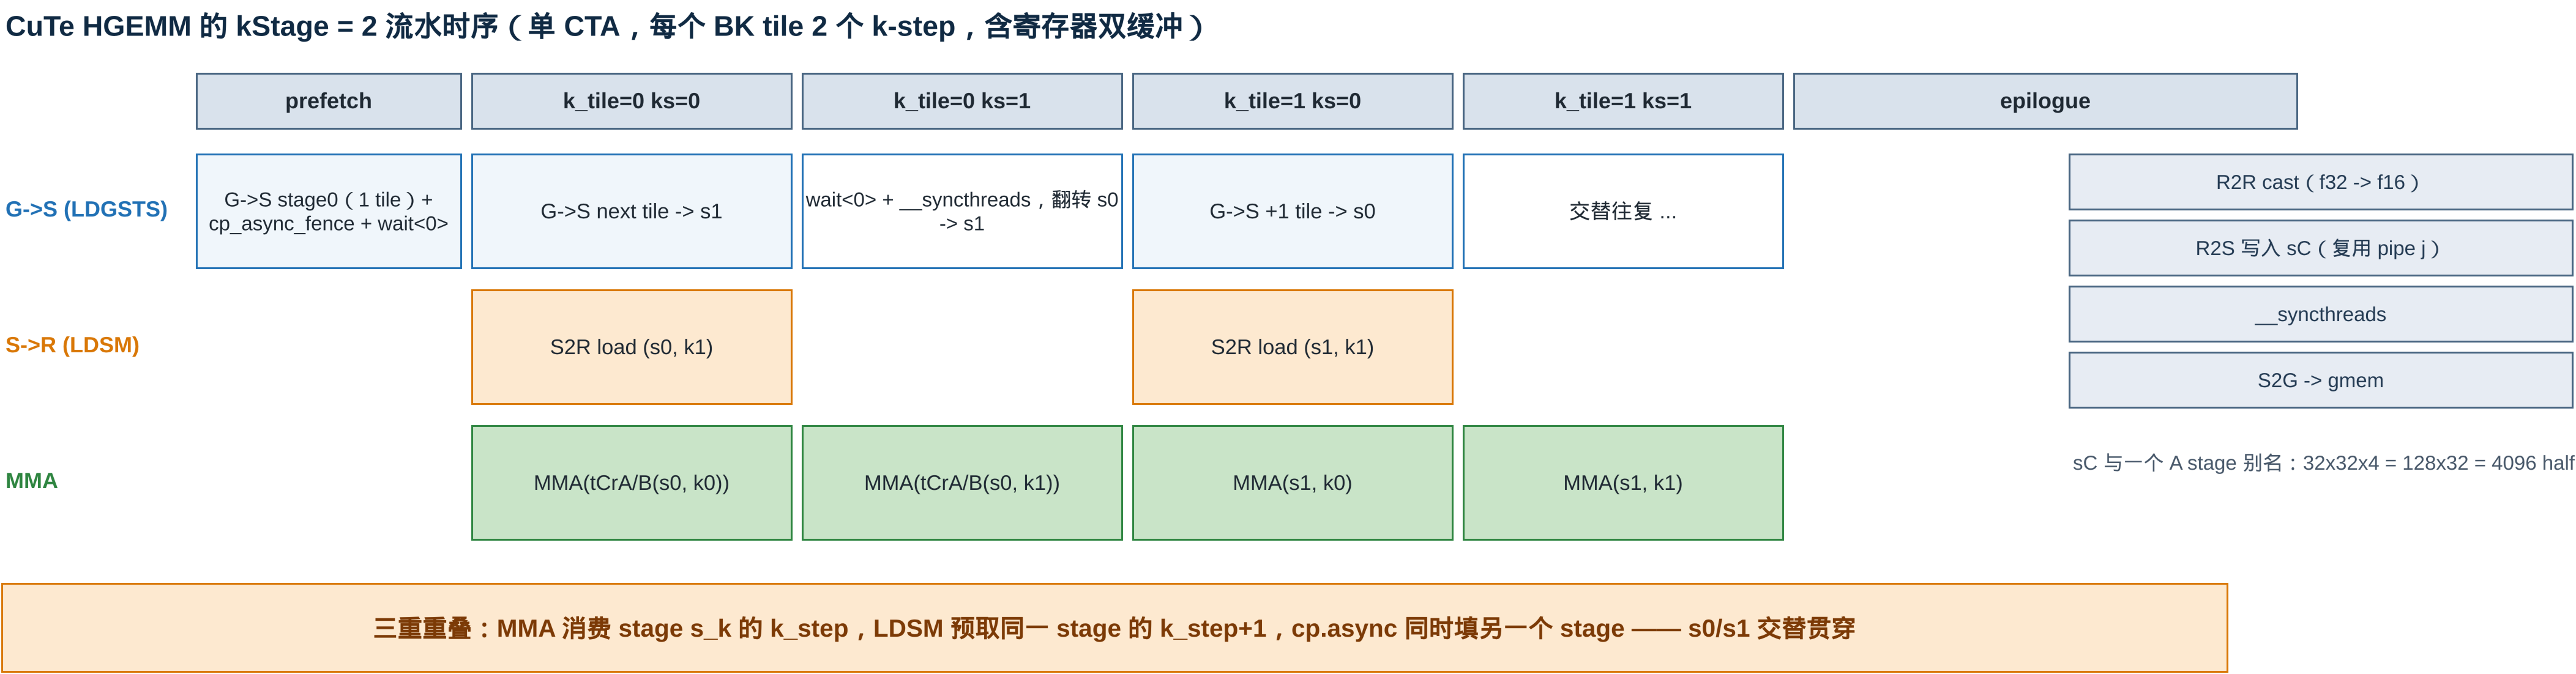
\includegraphics[width=0.95\textwidth]{figures/drawio/fig-24-2-kstage-pipeline/fig-24-2.png}
\begin{tikzpicture}[font=\tiny, >=Stealth,
  hdr/.style={draw=gray!55, fill=gray!14, align=center, inner sep=1.5pt,
    font=\fontsize{4}{4.5}\selectfont},
  cB/.style={draw=tkBlue, fill=tkFillBlue, align=center, inner sep=1.5pt,
    font=\fontsize{4}{4.5}\selectfont},
  cW/.style={draw=tkBlue!50, fill=white, align=center, inner sep=1.5pt,
    font=\fontsize{4}{4.5}\selectfont},
  cO/.style={draw=tkOrange, fill=tkFillOrange, align=center, inner sep=1.5pt,
    font=\fontsize{4}{4.5}\selectfont},
  cG/.style={draw=tkGreen, fill=tkFillGreen, align=center, inner sep=1.5pt,
    font=\fontsize{4}{4.5}\selectfont},
  cEpi/.style={draw=gray!60, fill=gray!12, align=center, inner sep=1.5pt,
    font=\fontsize{4}{4.5}\selectfont},
]
  % 时间列边界：0 / 1.75 / 4.10 / 6.45 / 8.80 / 11.15；epilogue 列 11.55-14.55
  \node[hdr, text width=1.60cm] at (0.875,0.87) {prefetch};
  \node[hdr, text width=2.20cm] at (2.925,0.87) {k\_tile$=$0\\ks$=$0};
  \node[hdr, text width=2.20cm] at (5.275,0.87) {k\_tile$=$0\\ks$=$1};
  \node[hdr, text width=2.20cm] at (7.625,0.87) {k\_tile$=$1\\ks$=$0};
  \node[hdr, text width=2.20cm] at (9.975,0.87) {k\_tile$=$1\\ks$=$1};
  \node[hdr, text width=2.85cm] at (13.05,0.87) {epilogue};
  % 泳道一：G->S（cp.async 填 smem）
  \node[cB, text width=1.60cm] at (0.875,-0.675)
    {G$\to$S s0\\（1 tile）\\$+$ fence\\$+$ wait$\langle0\rangle$};
  \node[cB, text width=2.20cm] at (2.925,-0.675) {G$\to$S 下一 tile $\to$ s1};
  \node[cW, text width=2.20cm] at (5.275,-0.675)
    {wait$\langle0\rangle$ $+$ \texttt{\_\_syncthreads}\\翻转 s0 $\to$ s1};
  \node[cB, text width=2.20cm] at (7.625,-0.675) {G$\to$S $+1$ tile $\to$ s0};
  \node[cB, text width=2.20cm] at (9.975,-0.675) {交替往复 $\cdots$};
  % 泳道二：S->R（ldmatrix 双缓冲）
  \node[cO, text width=2.20cm] at (2.925,-2.095) {S2R load (s0, k1)};
  \node[cO, text width=2.20cm] at (7.625,-2.095) {S2R load (s1, k1)};
  % 泳道三：MMA
  \node[cG, text width=2.20cm] at (2.925,-3.515) {MMA(tCrA/B(s0, k0))};
  \node[cG, text width=2.20cm] at (5.275,-3.515) {MMA(tCrA/B(s0, k1))};
  \node[cG, text width=2.20cm] at (7.625,-3.515) {MMA(s1, k0)};
  \node[cG, text width=2.20cm] at (9.975,-3.515) {MMA(s1, k1)};
  % 泳道标签
  \node[anchor=east, text=tkBlue, font=\bfseries\fontsize{4}{4.5}\selectfont]
    at (-0.15,-0.675) {G$\to$S (LDGSTS)};
  \node[anchor=east, text=tkOrange, font=\bfseries\fontsize{4}{4.5}\selectfont]
    at (-0.15,-2.095) {S$\to$R (LDSM)};
  \node[anchor=east, text=tkGreen, font=\bfseries\fontsize{4}{4.5}\selectfont]
    at (-0.15,-3.515) {MMA};
  % epilogue 四步（右列，不与三泳道同行）
  \node[cEpi, text width=2.85cm] at (13.05,-0.475) {R2R cast（f32 $\to$ f16）};
  \node[cEpi, text width=2.85cm] at (13.05,-1.575) {R2S 写入 sC（复用 pipe j）};
  \node[cEpi, text width=2.85cm] at (13.05,-2.675) {\texttt{\_\_syncthreads}};
  \node[cEpi, text width=2.85cm] at (13.05,-3.775) {S2G $\to$ gmem};
  \node[align=center, font=\fontsize{4}{4.5}\selectfont, text width=3.4cm]
    at (13.05,-4.56) {sC 与一个 A stage 别名：\\32$\times$32$\times$4 $=$ 128$\times$32 $=$ 4096 half};
  % 底部：三重重叠
  \node[draw=tkOrange, fill=tkFillOrange, text=tkOrange!80!black, align=center,
    font=\fontsize{4.2}{4.8}\selectfont, text width=15.2cm, inner sep=2pt]
    at (6.7,-5.18)
    {三重重叠：MMA 消费 stage $s_k$ 的 k\_step，LDSM 预取同一 stage 的 k\_step$+1$，%
     cp.async 同时填另一个 stage —— s0/s1 交替贯穿};
\end{tikzpicture}
\caption{CuTe HGEMM 的 $k_{\mathrm{stage}}=2$ 流水时序（含寄存器双缓冲）。上：G$\to$S（LDGSTS）；中：S$\to$R（LDSM）；下：MMA。MMA 消费 stage $s_k$ 的 k\_step 时，LDSM 预取同一 stage 的 k\_step+1，cp.async 同时填另一个 stage——三重重叠；左端 prefetch 一个 tile，右端 epilogue（R2R $\to$ R2S $\to$ S2G，sC 与一个 A stage 别名：$32{\times}32{\times}4 = 128{\times}32 = 4096$ half）。}
\label{fig:24-2}
\end{figure}

\begin{figure}[htbp]
\centering
% was: 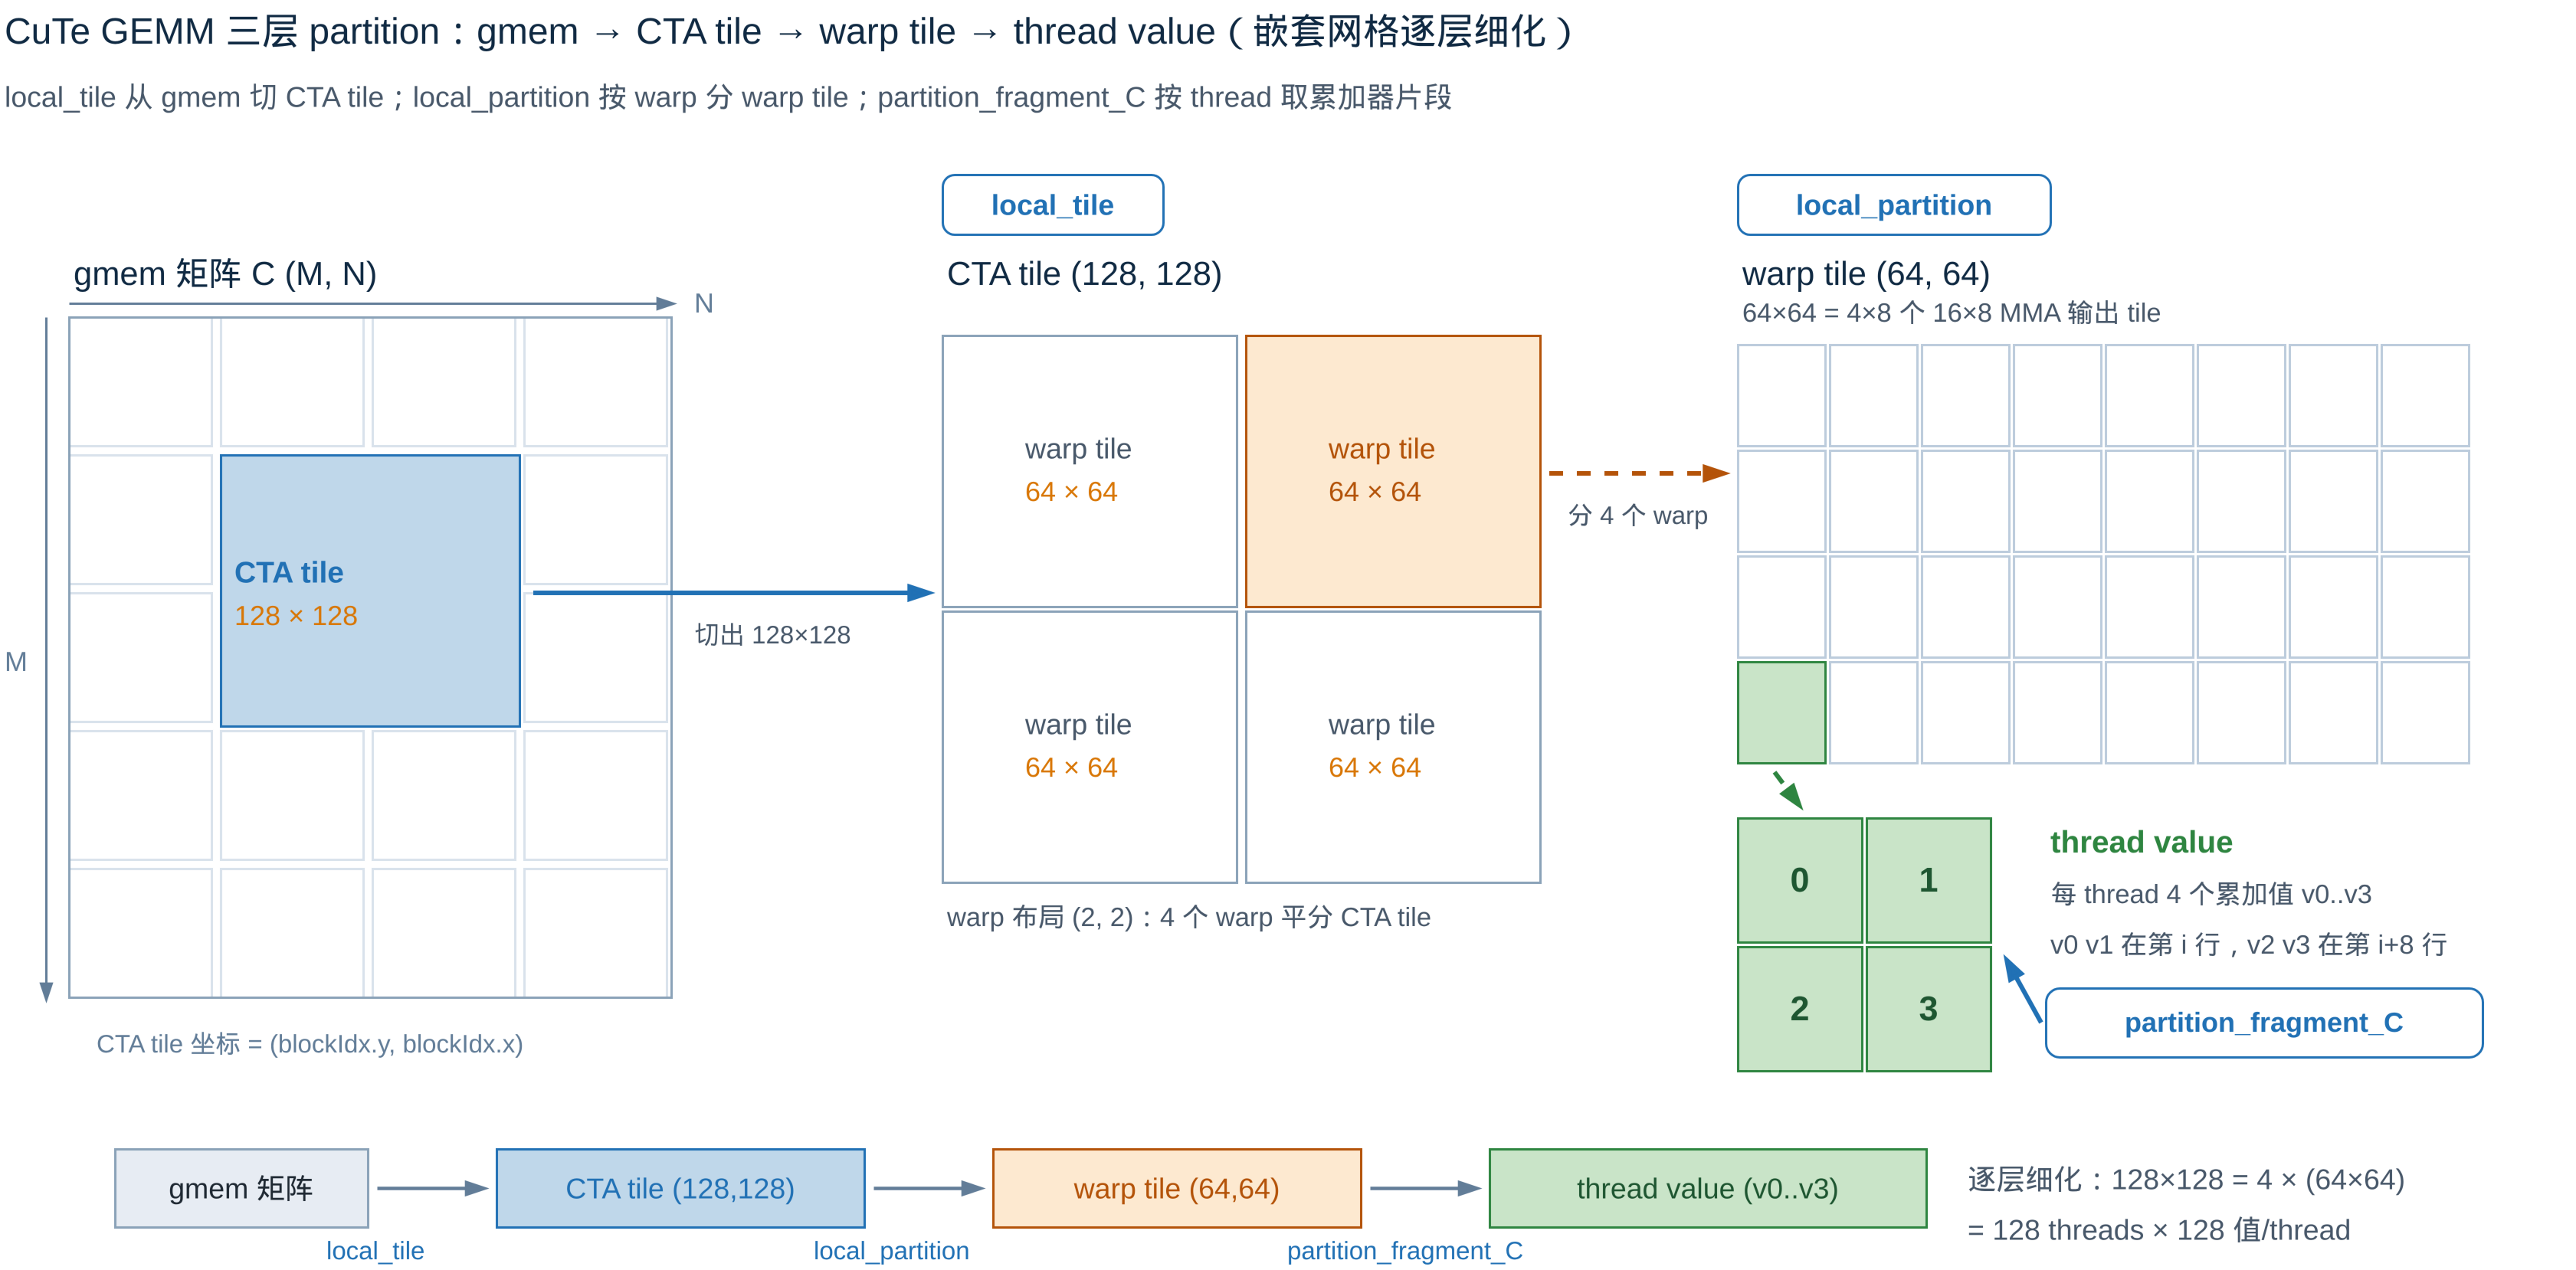
\includegraphics[width=0.95\textwidth]{figures/drawio/fig-24-3-gemm-3level-partition/fig-24-3.png}
\begin{tikzpicture}[font=\tiny, >=Stealth,
  pnl/.style={font=\fontsize{4.6}{5.2}\selectfont, inner sep=1pt},
  api/.style={draw=tkBlue, fill=tkFillBlue, rounded corners=1.5pt, text=tkBlue,
    align=center, inner sep=2pt, font=\fontsize{4}{4.5}\selectfont},
  small/.style={align=center, inner sep=1pt, font=\fontsize{4}{4.5}\selectfont},
]
  % 面板标题与 API 徽章（local_tile / local_partition 为所属层 API）
  \node[api] at (5.65,0.34) {local\_tile};
  \node[api] at (10.15,0.34) {local\_partition};
  \node[pnl, anchor=west] at (0.55,0.02) {gmem 矩阵 C (M, N)};
  \node[pnl, anchor=west] at (4.35,0.02) {CTA tile (128, 128)};
  \node[pnl, anchor=west] at (8.25,0.02) {warp tile (64, 64)};
  \node[small, anchor=west] at (8.25,-0.20) {64$\times$64 $=$ 4$\times$8 个 16$\times$8 MMA 输出 tile};
  % 面板 A：gmem 矩阵 4x5 格，CTA tile 覆盖中心 2x2 格
  \foreach \rr in {0,...,4} {
    \foreach \cc in {0,...,3} {
      \draw[gray!45, thin] ({0.55+0.60*\cc},{-0.45-0.54*\rr})
        rectangle ({0.55+0.60*\cc+0.60},{-0.45-0.54*\rr-0.54});
    }
  }
  \draw[gray!70, thick] (0.55,-0.45) rectangle (2.95,-3.15);
  \fill[tkFillBlue, draw=tkBlue, thick] (1.15,-0.99) rectangle (2.35,-2.07);
  \node[small] at (1.75,-1.37) {CTA tile};
  \node[small] at (1.75,-1.65) {128 $\times$ 128};
  \draw[->, gray!70, thin] (0.55,-0.30) -- (3.05,-0.30);
  \node[small, anchor=west] at (3.10,-0.30) {N};
  \draw[->, gray!70, thin] (0.32,-0.45) -- (0.32,-3.15);
  \node[small, anchor=center] at (0.16,-1.80) {M};
  \node[small, anchor=north, text width=2.60cm] at (2.00,-3.30)
    {CTA tile 坐标 $=$ (blockIdx.y, blockIdx.x)};
  % 面板 A -> B：local_tile 切出
  \draw[->, tkBlue, semithick] (3.05,-1.53) -- (4.35,-1.53);
  \node[small, text width=1.25cm] at (3.70,-1.72) {切出\\128$\times$128};
  % 面板 B：CTA tile = 2x2 warp tile（高亮右上角一个 warp）
  \foreach \rr in {0,...,1} {
    \foreach \cc in {0,...,1} {
      \pgfmathsetmacro{\xr}{4.35+1.30*\cc}
      \pgfmathsetmacro{\yr}{-0.45-1.12*\rr}
      \pgfmathtruncatemacro{\hi}{\cc - \rr}
      \ifnum\hi=1
        \fill[tkFillOrange] (\xr,\yr) rectangle (\xr+1.30,\yr-1.12);
        \draw[tkOrange, thick] (\xr,\yr) rectangle (\xr+1.30,\yr-1.12);
        \node[small, text=tkOrange!75!black] at (\xr+0.65,\yr-0.44) {warp tile};
        \node[small, text=tkOrange!75!black] at (\xr+0.65,\yr-0.70) {64 $\times$ 64};
      \else
        \draw[gray!60, thick] (\xr,\yr) rectangle (\xr+1.30,\yr-1.12);
        \node[small] at (\xr+0.65,\yr-0.44) {warp tile};
        \node[small] at (\xr+0.65,\yr-0.70) {64 $\times$ 64};
      \fi
    }
  }
  \node[small, anchor=north, text width=3.0cm] at (5.65,-2.78)
    {warp 布局 (2, 2)：4 个 warp 平分 CTA tile};
  % 面板 B -> C：local_partition 分给单个 warp
  \draw[->, dashed, tkOrange, semithick] (7.05,-1.10) -- (8.25,-1.10);
  \node[small, text width=1.2cm] at (7.65,-1.30) {分 4 个\\warp};
  % 面板 C：warp tile = 4x8 个 16x8 MMA 输出格；左下格放大为 thread 累加片段
  \foreach \rr in {0,...,3} {
    \foreach \cc in {0,...,7} {
      \draw[gray!45, thin] ({8.25+0.40*\cc},{-0.45-0.36*\rr})
        rectangle ({8.25+0.40*\cc+0.40},{-0.45-0.36*\rr-0.36});
    }
  }
  \fill[tkFillGreen, draw=tkGreen, thick] (8.25,-1.89) rectangle (8.65,-1.53);
  \draw[gray!70, thick] (8.25,-0.45) rectangle (11.45,-1.89);
  \draw[->, dashed, tkGreen, semithick] (8.45,-1.96) -- (8.62,-2.30);
  \foreach \rr in {0,...,1} {
    \foreach \cc in {0,...,1} {
      \pgfmathsetmacro{\xb}{8.25+0.55*\cc}
      \pgfmathsetmacro{\yb}{-2.35-0.55*\rr}
      \pgfmathtruncatemacro{\vi}{2*\rr+\cc}
      \fill[tkFillGreen, draw=tkGreen, thick] (\xb,\yb) rectangle (\xb+0.50,\yb-0.50);
      \node[font=\fontsize{4.6}{5.2}\selectfont, text=tkGreen!75!black]
        at (\xb+0.25,\yb-0.25) {v\vi};
    }
  }
  \node[font=\bfseries\fontsize{4}{4.5}\selectfont, text=tkGreen, anchor=west]
    at (9.40,-2.52) {thread value};
  \node[small, anchor=west] at (9.40,-2.76) {每 thread 4 个累加值 v0..v3};
  \node[small, anchor=west] at (9.40,-3.00) {v0 v1 在第 $i$ 行，v2 v3 在第 $i{+}8$ 行};
  \node[api, text width=1.95cm] at (10.50,-3.62) {partition\_fragment\_C};
  \draw[->, tkBlue, semithick] (9.46,-3.55) -- (9.30,-3.42);
  % 底部层级链：四层对象 + 三个 API
  \node[draw=gray!65, fill=gray!12, align=center, inner sep=2pt,
    font=\fontsize{4.2}{4.8}\selectfont, text width=1.50cm] at (1.65,-4.58) {gmem 矩阵};
  \node[draw=tkBlue, fill=tkFillBlue, text=tkBlue, align=center, inner sep=2pt,
    font=\fontsize{4.2}{4.8}\selectfont, text width=2.20cm] at (4.70,-4.58) {CTA tile (128,128)};
  \node[draw=tkOrange, fill=tkFillOrange, text=tkOrange!80!black, align=center,
    inner sep=2pt, font=\fontsize{4.2}{4.8}\selectfont, text width=2.20cm]
    at (8.10,-4.58) {warp tile (64,64)};
  \node[draw=tkGreen, fill=tkFillGreen, text=tkGreen!80!black, align=center,
    inner sep=2pt, font=\fontsize{4.2}{4.8}\selectfont, text width=2.60cm]
    at (11.70,-4.58) {thread value (v0..v3)};
  \draw[->, gray!70, semithick] (2.44,-4.58) -- (3.56,-4.58);
  \draw[->, gray!70, semithick] (5.84,-4.58) -- (6.96,-4.58);
  \draw[->, gray!70, semithick] (9.24,-4.58) -- (10.36,-4.58);
  \node[small, text=tkBlue] at (3.00,-4.86) {local\_tile};
  \node[small, text=tkBlue] at (6.40,-4.86) {local\_partition};
  \node[small, text=tkBlue] at (9.80,-4.86) {partition\_fragment\_C};
  \node[small, anchor=west, text width=2.00cm] at (13.15,-4.45)
    {逐层细化：\\128$\times$128 $=$ 4 $\times$ (64$\times$64)\\
     $=$ 128 threads $\times$ 128 值/thread};
\end{tikzpicture}
\caption{CuTe GEMM 的三层 partition：\texttt{local\_tile} 以 \texttt{\allowbreak{}(block\allowbreak{}Idx.\allowbreak{}y,\allowbreak{} block\allowbreak{}Idx.\allowbreak{}x)} 为坐标从 gmem 切出 CTA tile $(128,128)$；warp 布局 $(2,2)$ 下 \texttt{local\_\allowbreak{}partition} 平分给 4 个 warp 得 $(64,64)$；warp tile 由 $4\times8$ 个 $16\times8$ atom 铺满，\texttt{partition\_\allowbreak{}fragment\_\allowbreak{}C} 为每 thread 生成累加器片段（单 MMA tile 内 $2\times2$ 四值，v0/v1 在第 $i$ 行、v2/v3 在第 $i+8$ 行）。层级换算 $128\times128=4\times(64\times64)=128$\,threads$\times128$ 值/thread。重建自 @reed《cute 之 简单 GEMM 实现》（示意图为经典 4-warp/$64\times64$ 配置；本章 kernel 实为 tile $32\times32$、warp $16\times16$，层级方法相同）。}
\label{fig:24-3}
\end{figure}

\section{性能分析}

本章没有为 CuTe HGEMM 单独建 bench（Phase~7c 的集成数据由 \texttt{bench/bench\_leetcuda.cu}
的 \texttt{--bench} 统一采集）。这里只给三条可核验的定量结论：

\begin{enumerate}
  \item \textbf{正确性}：最小测试在 $128\times256\times64$（F16 累加）与
        $128\times128\times64$（F32 累加）两组形状上分别以
        \texttt{TOL\_F16ACC}$=5\times10^{-2}$、\texttt{TOL\_F32ACC}$=10^{-3}$
        判定通过（第~\ref{sec:24-minitest}~节给出实测 \texttt{max\_abs\_err}）。
  \item \textbf{寄存器压力}：\texttt{ptxas -v} 实测两种配置的寄存器数与 stack
        使用（实测值见本节的实践须知），核对源码注释里\textbf{均 0 spill}的说法。
  \item \textbf{smem 占用}：式~\eqref{eq:24-smem} 的 48\,KiB 由
        \texttt{cosize\allowbreak{}(Smem\allowbreak{}Layout\allowbreak{}A) + cosize\allowbreak{}(Smem\allowbreak{}Layout\allowbreak{}B)} 在
        编译期算出。同一个常量既决定 \texttt{cuda\allowbreak{}Func\allowbreak{}Set\allowbreak{}Attribute} 的实参，也决定
        occupancy 上限。$B_N$ 降到 128（F32 累加）时它同步降到 32\,KiB，
        精度换占用的取舍是类型参数的直接后果。
\end{enumerate}

\paragraph{实践须知：两处源码注释的性能口径}\label{sec:24-kaogu}

\begin{itemize}
  \item \textbf{$B_N$ 随累加精度切换的寄存器断言}（hgemm.cuh L1229--1230）：
        注释称\textbf{F16 acc 用 256（$128\times256$ tile，0 spill）；F32 acc 用 128
        （$128\times128$ tile，0 spill）。F32 $+$ $B_N{=}256$ 会产生
        $\sim$1\,KB spill（254 reg），性能下降 3--8 倍}。用
        \texttt{nvcc -Xptxas -v} 编译本 wrapper 的两种实例化（与本章测试同源）
        实测：$B_N{=}256$/F16 用 254 个寄存器、$B_N{=}128$/F32 用 226 个，
        \textbf{两者 stack frame 均为 0 字节}（0 spill stores / 0 spill loads），
        与注释前两句一致。
  \item 注释第三句描述的组合在本 wrapper 里\textbf{不可达}：\texttt{kBN} 由
        \texttt{kAccF32} 单向决定，F32 累加永远配不到 $B_N=256$，属于手工改坏
        才会遇到的反例。测量值本身有效（它是 $B_N{=}256$ 那一档的
        254\,reg），只是不该被读成\textbf{本 kernel 的第三种配置}；复现方法见
        第~\ref{sec:24-minitest}~节动手实验第 3 条。
  \item \textbf{代码量对照}（hgemm.cuh L803--805）：注释写\textbf{手写 $\sim$200 行 /
        CuTe $\sim$80 行}。按同口径实测（去注释、去空行）：手写 Phase~7b 为
        151 行、Phase~7b-3 为 235 行，CuTe kernel 本体为 118 行（另有 launch
        wrapper 86 行）。注释给的是量级估计，方向正确（CuTe 版确实更短），但
        \textbf{$\sim$80 行}低估了约三成；本章一律以实测数字为准
        （图~\ref{fig:24-1}）。
\end{itemize}

\paragraph{实测性能：CuTe Swizzle 家族 vs cuBLAS}\label{sec:ch24-perf}

前面几条验证的都是本章自己给的数字，再给一组对外的对照：第~\ref{ch:20}--\ref{ch:23}~章
铺垫的 layout 代数、\texttt{TiledCopy}、\texttt{TiledMMA}、swizzle 组合子落到
真实负载上究竟值多少？用 \texttt{leetcuda\_\allowbreak{}bench\_\allowbreak{}sm120a.\allowbreak{}bin} 的
\texttt{--bench --bench-all} 在 RTX PRO 5000（sm\_120，110 SM，CUDA 13.2）上实测
$M{=}N{=}K{=}8192$ 的 fp16 HGEMM，CuTe Swizzle 家族七个配置见
表~\ref{tab:ch24-perf}：F16Acc 档追平乃至超越 cuBLAS f16（分母为同轮 cuBLAS
f16 的 246.5\,TFLOPS，本家族 0.99$\sim$1.08$\times$，最高 1.08$\times$），F32Acc 档
对比 cuBLAS f32（164.2\,TFLOPS）达 1.48$\times$。七个配置的 Max Err 全部为
$0.000\mathrm{e}{+}00$，逐位零误差。这些地址算术在编译期被类型系统全部折叠成
最终指令，实测说明这套抽象是零开销的。

\begin{table}[H]
\centering
\caption{HGEMM CuTe Swizzle 实测（RTX PRO 5000，M=N=K=8192，fp16）}
\label{tab:ch24-perf}
\footnotesize
\setlength{\tabcolsep}{4pt}
\begin{tabular}{lrr}
\toprule
Kernel & Max Err & TFLOPS/cuBLAS（加速比） \\
\midrule
HGEMM CuTe Swizzle (S=2, BLK\_SW=0, F16Acc) & 0.000e+00 & 243.0/246.5 (0.99x) \\
HGEMM CuTe Swizzle (S=2, BLK\_SW=0, F32Acc) & 0.000e+00 & 201.3/164.2 (1.23x) \\
HGEMM CuTe Swizzle (S=2, BLK\_SW=1, F16Acc) & 0.000e+00 & 250.2/246.5 (1.01x) \\
HGEMM CuTe Swizzle (S=2, BLK\_SW=1, F32Acc) & 0.000e+00 & 226.0/164.2 (1.38x) \\
HGEMM CuTe Swizzle (S=3, BLK\_SW=0, F16Acc) & 0.000e+00 & 257.2/246.5 (1.04x) \\
HGEMM CuTe Swizzle (S=3, BLK\_SW=1, F16Acc) & 0.000e+00 & 265.9/246.5 (1.08x) \\
HGEMM CuTe Swizzle (S=3, BLK\_SW=1, F32Acc) & 0.000e+00 & 242.4/164.2 (1.48x) \\
\bottomrule
\end{tabular}
\end{table}

CuTe 版\textbf{不承诺}比手写版更快。两者的指令序列高度重合
（SASS 层面都是 \texttt{LDGSTS} $+$ \texttt{LDSM} $+$ \texttt{HMMA}），差别在
编译期把地址算术折叠掉、以及让 kernel 作者少写上百行易错的表达式。真正的加速
来自第~\ref{ch:12}~章那样的算法级决策（swizzle 档位、block swizzle、
寄存器双缓冲）；CuTe 的价值是让这些决策更容易表达、检查与复用。

\section{常见坑}

\begin{enumerate}
  \item B 必须转置传入。式~\eqref{eq:24-tn} 的 TN 语义要求 \texttt{Bptr} 指向
        $B^{\mathsf T}[N,K]$ 的 row-major 存储。直接把 row-major 的 $B[K,N]$
        传进去不会报错，只会算错。最小测试在 host 侧显式构造转置。
  \item 没有 tile 内 predication。kernel 只有 CTA 级边界判断，调用方必须保证
        $M \% B_M = 0$、$N \% B_N = 0$、$K \% B_K = 0$；这也决定了本章测试
        形状取 $128/256/64$（$M=N=K=64$ 用不了：$B_M=128$）。
  \item $B_N$ 与累加精度绑定。\texttt{k\allowbreak{}Acc\allowbreak{}F32=\allowbreak{}true} 时 $B_N$ 自动降到 128；
        手工把 F32 累加配到 $B_N=256$（本 wrapper 不可达的组合）会让累加器
        超出可用寄存器、溢出到 local memory（第~\ref{sec:24-kaogu}~节）。
  \item 动态 smem 必须显式提额。\texttt{cuda\allowbreak{}Func\allowbreak{}Set\allowbreak{}Attribute} 在 wrapper 里、
        launch 之前；漏掉它只会在 $k_{\mathrm{stage}}$ 较大时启动失败。
  \item BlockSwizzle 改变 grid 维度。开关打开后 grid 是 3D 且 \texttt{BX} 要按
        \texttt{BZ} 折算；只改 kernel 模板参数而不改 host 侧 grid 会索引错 block。
  \item epilogue 别漏 \texttt{\_\allowbreak{}\_\allowbreak{}syncthreads\allowbreak{}()}。R2S 与 S2G 之间必须汇合：
        S2G 读的是其它线程刚写入 sC 的数据；漏掉会得到大部分正确、偶发错误的
        结果。
  \item $k_{\mathrm{stage}}$ 与 smem 的联动。$k_{\mathrm{stage}}$ 从 2 加到 3 会把
        式~\eqref{eq:24-smem} 的 A$+$B 部分抬高 50\%；\texttt{kShmSize} 与
        \texttt{cuda\allowbreak{}Func\allowbreak{}Set\allowbreak{}Attribute} 会自动跟着变，但 occupancy 会下降，
        这是改一个模板参数的连带代价。
\end{enumerate}

\section{面试要点速查}

\begin{enumerate}
  \item \textbf{Q}：CuTe 版 HGEMM 比手写版短在哪？
        \textbf{A}：短在地址算术：smem 寻址、swizzle、\texttt{ldmatrix} lane 映射、
        epilogue shuffle 四类表达式全部由类型推导取代；流水线的
        同步逻辑（fence/wait/计数器）两边一样要手写。
  \item \textbf{Q}：\texttt{cute::gemm} 自动展开了哪些循环？
        \textbf{A}：对 $(V,M,K)\times(V,N,K)$ 输入，
        \texttt{MMA\_M}$\times$\texttt{MMA\_N}$\times$\texttt{MMA\_K}
        都会被展开。外层 K-tile 的搬运循环仍需手写；本章显式
        \texttt{k\_step} 则服务于寄存器双缓冲，不是 \texttt{gemm} 的能力限制。
  \item \textbf{Q}：为什么 $B_K=32$ 而不是 64？
        \textbf{A}：smem 预算与切片粒度的折中：$B_K=32$ 时
        $n_{k\text{-step}}=2$、A$+$B 双 stage 占 48\,KiB；$B_K$ 翻倍会同步
        抬高 smem 并挤压 occupancy。
  \item \textbf{Q}：\texttt{make\_\allowbreak{}tiled\_\allowbreak{}copy\_\allowbreak{}A} 为什么不需要指定
        ThrLayout？
        \textbf{A}：它从 \texttt{tiled\_mma} 反推：S$\to$R 的线程映射必须与
        MMA fragment 的分布共形，两者是同一事实的两种表述。
  \item \textbf{Q}：epilogue 为什么经 smem 中转？
        \textbf{A}：累加器 fragment 的寄存器分布不适合直接宽写 gmem；经 smem
        做一次 CTA 范围的数据重组（R2S $+$ S2G），才能用 128-bit 宽写，
        并且避免手写跨 lane 的 shuffle 编排。
  \item \textbf{Q}：换成 F32 累加要动哪些地方？
        \textbf{A}：换 atom（\texttt{SM80\_\allowbreak{}16x8x16\_\allowbreak{}F32\allowbreak{}F16\allowbreak{}F16\allowbreak{}F32\_\allowbreak{}TN}），
        $B_N$ 随之降到 128，其余（C scratchpad pipe、R2S cast、S2G 宽写）
        由同一套类型推导覆盖，这是类型即配置的收益。
\end{enumerate}

\section{最小测试与动手实验}\label{sec:24-minitest}

\texttt{book/\allowbreak{}tests/\allowbreak{}ch24\_\allowbreak{}hgemm\_\allowbreak{}cute.cu} 的逻辑照抄 \texttt{bench/hgemm.cu}
L192 的 \texttt{test\_\allowbreak{}hgemm\_\allowbreak{}cute}，但按本书测试规范改造：参考值换成
\textbf{CPU fp64 三重循环}（不依赖 cuBLAS），判定走 \texttt{book\_check}
容差三档。测试跑两组配置：

\begin{itemize}
  \item 第一组：\texttt{launch\_\allowbreak{}hgemm\_\allowbreak{}mma\_\allowbreak{}stages\_\allowbreak{}tn\_\allowbreak{}cute\allowbreak{}<half, 2, 0, false>}，
        $M{=}128,N{=}256,K{=}64$，容差 \texttt{TOL\_F16ACC}$=5\times10^{-2}$；
  \item 第二组：\texttt{launch\_\allowbreak{}hgemm\_\allowbreak{}mma\_\allowbreak{}stages\_\allowbreak{}tn\_\allowbreak{}cute\allowbreak{}<half, 2, 0, true>}，
        $M{=}128,N{=}128,K{=}64$，容差 \texttt{TOL\_F32ACC}$=10^{-3}$。
\end{itemize}

规模约束来自 kernel 的整除要求（$M\%128=0$、$N\%B_N=0$、$K\%32=0$），同时满足
BOOK\_PLAN §6\textbf{CPU 参考规模 $\le 512$}的时限约束。编译与运行：

\begin{lstlisting}[style=console]
cd kernels/interview/book/tests
CUDA_VISIBLE_DEVICES=6 ./build_tests.sh --arch sm_120a --ch ch24
\end{lstlisting}

本机运行输出（RTX PRO 5000，CUDA 13.2，CUTLASS v4.6.1，2026-09-11）：

\begin{lstlisting}[style=console]
== ch24_hgemm_cute.cu (sm_120a)
PASS HGEMM CuTe F16Acc 128x256x64: max_abs_err=4.376e-04 (tol=5.0e-02)
PASS HGEMM CuTe F32Acc 128x128x64: max_abs_err=2.897e-04 (tol=1.0e-03)
ALL OK
\end{lstlisting}

两组输入的随机数幅度缩到 $\pm0.25$：fp16\textbf{输出}的舍入误差量级是
$|C|\cdot2^{-11}$，只有把 $|C|$ 压在 $2$ 附近，$10^{-3}$ 这条容差才是在
检验\textbf{累加精度}而不是\textbf{输出量化}。带上 \texttt{bench} 参数还能跑一版
吞吐计时（$K{=}64$ 的规模只有微秒级，被 launch 开销主导，不构成性能结论；
端到端吞吐对照见第~\ref{sec:ch24-perf}~节）。

代码量的统计口径（图~\ref{fig:24-1} 的数字）只统计非空、非纯注释行，
用一条 \texttt{awk} 命令即可复现。动手实验建议三条：

\begin{enumerate}
  \item 把 \texttt{Stages} 从 2 改成 3，观察 smem 涨到 72\,KiB 量级、
        \texttt{cuda\allowbreak{}Func\allowbreak{}Set\allowbreak{}Attribute} 的实参随之变化。
  \item 把 \texttt{Block\allowbreak{}Swizzle} 置 1 并改 host 侧 grid 为 3D，用同一组形状
        验证结果不变（只影响 L2 局部性，不影响正确性）。
  \item 把 \texttt{kAccF32} 置 true 但手工把 \texttt{kBN} 改回 256，用
        \texttt{-Xptxas -v} 看 spill 报告，复现第~\ref{sec:24-kaogu}~节提到的反例。
\end{enumerate}

\section*{延伸阅读}

\begin{itemize}
  \item @reed《cute 之 简单 GEMM 实现》，
        \url{https://zhuanlan.zhihu.com/p/667521327}
        （从零搭 CuTe GEMM 的三步骨架，本章第~\ref{sec:24-step1}~节按它展开）。
  \item @reed《cute 之 GEMM 流水线》，
        \url{https://zhuanlan.zhihu.com/p/665082713}
        （multistage 流水的 CuTe 写法与\textbf{流水线不属于 cute}的结论，本章
        第~\ref{sec:24-step2}~节按它展开）。
  \item @reed《cute 之 高效 GEMM 实现》，
        \url{https://zhuanlan.zhihu.com/p/675308830}
        （访存/计算/尾阶段高效与主机端类型清单，对应本章
        第~\ref{sec:24-step3a}、\ref{sec:24-step3b}~节）。
  \item @竹熙佳处《写给大家看的 CuTe 教程：async pipeline》，
        \url{https://zhuanlan.zhihu.com/p/2024832248386528275}
        （可对照本章\textbf{流水线仍要手写}的结论）；
  \item @进击的Killua《CUTLASS CuTe 实战（一）：基础》，
        \url{https://zhuanlan.zhihu.com/p/690703999}
        （Tensor 常用 API 速查，适合边看本章代码边查手册）。
\end{itemize}

% ch25-cute-flash-attn.tex — CuTe 应用（二）：FlashAttention 三实现对照（agent-ch25 撰写，2026-09-11）
% 源码区间（anchors.yaml ch25）：flash_attn.cuh L2196-3488（NOTES_V2_ENABLE_CUTE 宏块）
% \url 由 book.tex 的 hyperref 提供；单章独立编译时降级为可断行的 \ttfamily
\makeatletter
\providecommand{\urlchbrk}[1]{\@tfor\next:=#1\do{\next\allowbreak}}
\makeatother
\providecommand{\url}[1]{{\ttfamily\urlchbrk{#1}}}
\chapter{CuTe 应用（二）：FlashAttention 三实现对照}\label{ch:25}

\section{本章导读}

第~\ref{ch:16}--\ref{ch:18}~章我们用手写地址算术实现了三代 FlashAttention：
FA2 的 Split-Q + cp.async 多级流水（flash\_attn.cuh L5--790）、FA2 的 TMA + warp
specialization（L792--1440）、FA3 的双 consumer warpgroup（L1441--2192）。三代实现
都在做同一件事：把 $S=QK^\top$、online softmax、$O=PV$ 三段落进张量核与搬运
流水之间；但每一代都要重写一遍 Q/K/V 的 smem 布局、fragment 的 lane 映射、
ldmatrix 的地址算术与屏障协议。这不是作者偷懒：布局事实在 C++/PTX 里没有
独立的落脚点，swizzle 常量、lane 位段、寄存器编号只能以裸算术的形式与计算
逻辑混写在一起。

本章问一个具体的问题：把这些布局事实搬进类型之后，同一段 attention 会长什么
样？答案是同一文件第四个区段的四个 CuTe 实现（L2196--3488，
\texttt{NOTES\_\allowbreak{}V2\_\allowbreak{}ENABLE\_\allowbreak{}CUTE} 宏块）。它们不是四份互不相干的代码，而是
同一个算法的三级搭建：实现 1
\texttt{flash\_\allowbreak{}attn\_\allowbreak{}mma\_\allowbreak{}stages\_\allowbreak{}split\_\allowbreak{}q\_\allowbreak{}cute}（cp.async + 统一流水，256 线程）最朴素，
组装方式照 @reed《cute 之 简单 GEMM 实现》的 Tensor $\to$ \texttt{local\_tile}
$\to$ partition $\to$ copy/gemm 四步走：数据怎么切、怎么分给线程、怎么搬、
怎么算，一一对应到 CuTe 抽象；实现 2
\texttt{flash\_\allowbreak{}attn\_\allowbreak{}tma\_\allowbreak{}mma\_\allowbreak{}ws\_\allowbreak{}split\_\allowbreak{}q\_\allowbreak{}cute}（TMA + producer/consumer 分工，
384 线程）在同一个算法上把搬运与计算解耦；实现 3
\texttt{flash\_\allowbreak{}attn\_\allowbreak{}3\_\allowbreak{}tma\_\allowbreak{}mma\_\allowbreak{}ws\_\allowbreak{}split\_\allowbreak{}q\_\allowbreak{}cute} 进一步采用 FA3 式双 consumer
（奇偶拆 KV + 终态归并）。第四个实现
\texttt{flash\_\allowbreak{}attn\_\allowbreak{}3\_\allowbreak{}cute\_\allowbreak{}tma\_\allowbreak{}copy\_\allowbreak{}smoke}（42 行）不是 attention，而是
一条 TMA 搬运链路的自检闭环，用来先把搬运与计算解耦，再单独排查。这是
Part~IV 的倒数第二章，也是抽象换代码量这条主线在 attention 上的完整样本。

本章的组织以动机为线：三级搭建逐级回答上一级留下的问题：实现 1
的浪费在哪、为什么实现 2 要把搬运拆出去、为什么实现 3 要拆 KV。四个实现共享
同一组编译期布局类型（\texttt{Flash\allowbreak{}Attn2\allowbreak{}Cu\allowbreak{}Te\allowbreak{}Traits} /
\texttt{Flash\allowbreak{}Attn3\allowbreak{}Cu\allowbreak{}Te\allowbreak{}Traits}）与五个 kernel 级工具函数，
这是第~\ref{ch:22}~章 TiledMMA 与 fragment 在真实 kernel 里的落点：

\begin{itemize}[itemsep=1pt,topsep=2pt]
  \item \texttt{convert\_\allowbreak{}layout\_\allowbreak{}acc\_\allowbreak{}rowcol} 与 \texttt{convert\_\allowbreak{}layout\_\allowbreak{}acc\_\allowbreak{}Aregs}
        是两个 fragment 重排函数（25.3.3/25.3.4 节）；
  \item \texttt{convert\_\allowbreak{}type}、\texttt{gemm\_ss}、\texttt{gemm\_rs} 负责类型转换与
        两个 GEMM 调用范式（25.4.1 节）。
\end{itemize}

五个函数里，\texttt{convert\_\allowbreak{}layout\_\allowbreak{}acc\_\allowbreak{}Aregs} 单独成节：$P$
（softmax 后的分数矩阵）要从 QK 的累加器变成 PV 的左操作数，@竹熙佳处
《写给大家看的 CuTe 教程：Layout Compose \& Inverse》讨论的正是这个场景。

\textbf{前置章节}：第~\ref{ch:17}~章（手写 TMA+WS 的 mbarrier 协议）、
第~\ref{ch:18}~章（FA3 双 consumer 与 merge）、第~\ref{ch:21}~章
（Tensor 与 TiledCopy：G2S/S2R 分工）、第~\ref{ch:22}~章（TiledMMA、EURepeat、
fragment 与 rowcol 变换）。\textbf{源码区间}：flash\_attn.cuh L2196--3488。
\textbf{编译宏}：\texttt{NOTES\_\allowbreak{}V2\_\allowbreak{}ENABLE\_\allowbreak{}CUTE}（四个实现都需要 TMA 或
cp.async 的 CuTe 抽象；sm80+ 可编）；后三个实现另需
\texttt{NOTES\_\allowbreak{}V2\_\allowbreak{}ENABLE\_\allowbreak{}TMA\_\allowbreak{}MMA\_\allowbreak{}WS}（TMA 指令，sm90+ 硬件）。
本节默认实例化取 $D\in\{64,128\}$、$B_r\in\{64,128\}$、$B_c=64$。
配套最小测试 \texttt{book/\allowbreak{}tests/\allowbreak{}ch25\_\allowbreak{}fa\_\allowbreak{}cute.\allowbreak{}cu}（三种形状的端到端正确性）。

\section{问题与动机}

先摊开手写版的维护面。第~\ref{ch:16}~章的 FA2 kernel 共 564 行有效代码，其中与
布局事实直接相关的至少有五类，且每一类都以裸地址算术的形式出现：

\begin{enumerate}
  \item \textbf{smem 行距与 padding}：$kSmemStrideQ/K/V = D+\mathrm{pad}$，
        pad 取 8 个 half 使 ldmatrix 的 8 行起始 bank 铺满 32 个 bank；
        $pk$ 与 $kPad$ 的组合还决定走 XOR swizzle 还是 padding 路径；
  \item \textbf{ldmatrix 的 lane 映射}：Q 用 \texttt{ldmatrix.x4}、
        K 用 \texttt{ldmatrix.x2}、V 用 \texttt{ldmatrix.\allowbreak{}x2.trans}，
        三者的行/列由 \texttt{lane} 的位段手工拼出；
  \item \textbf{fragment 的寄存器编号}：$R\_S[8][2]$、$R\_O/R\_D[8][2]$
        是哪个寄存器对应矩阵哪个元素的硬编码答案，4-lane 归约宽度
        （\texttt{warp\_\allowbreak{}reduce\allowbreak{}<4>}）也是从这套编号推出来的；
  \item \textbf{搬运粒度的地址划分}：256 线程协作加载时
        \texttt{load\_\allowbreak{}smem\_\allowbreak{}Q\_\allowbreak{}Br =\allowbreak{} tid/\allowbreak{}2} 这类映射；
  \item \textbf{屏障计数}：producer/consumer 的 arrive\_count（第~\ref{ch:17}~章
        的 257 协议、第~\ref{ch:18}~章的 per-WG 129）。
\end{enumerate}

第~\ref{ch:20}~章已经论证过这五类事实的联动代价：改一个 tile 尺寸，至少三处
要跟着改，且错误是静默的。CuTe 版的答案是把它们全部收进
\textbf{编译期类型}：smem 布局是 \texttt{tile\_\allowbreak{}to\_\allowbreak{}shape} 的返回类型、fragment
布局是 \texttt{partition\_\allowbreak{}fragment\_\allowbreak{}A/B/C} 的返回类型、搬运是
\texttt{TiledCopy} 的 TV 划分、连 V 的转置视图都是
\texttt{composition} 表达式的类型。kernel 正文里只剩三类语句：
数据流（\texttt{copy}/\texttt{gemm}）、同步（barrier / \texttt{cp.\allowbreak{}async.\allowbreak{}wait}）
与 online softmax 的标量运算。抽象掉了什么，可以逐项核对：\textbf{坐标计算}
收进 \texttt{local\_tile}/\texttt{partition} 的类型、\textbf{fragment 手工索引}
收进 \texttt{partition\_\allowbreak{}fragment} 的返回布局、\textbf{拷贝指令的选择}
收进 \texttt{TiledCopy} 的原子类型（G2S 选 cp.async 还是 TMA、S2R 选哪个
ldmatrix 形态）；三件事都不再出现在 kernel 正文里。

量化一下收益。表~\ref{tab:25-code} 用区间总行数除以去注释空行的有效代码行数，
对照三对实现（手写版区间与 CuTe 版区间都取自同一文件，统计口径一致：行以
\texttt{\textbackslash n} 计，注释行指以 \texttt{//} 开头的行）。

\begin{table}[htbp]
\centering
\caption{手写版与 CuTe 版的有效代码行数对照（flash\_attn.cuh，2026-09-11 统计）。
「结构件」指 FA2/FA3 traits 与五个工具函数，它们被后四个实现共享。}
\label{tab:25-code}
\begin{tabular}{llrr}
\toprule
实现 & 区间 & 总行数 & 有效代码行 \\
\midrule
FA2 手写（Split-Q + cp.async） & L5--790 & 786 & 564 \\
FA2 手写（TMA + WS） & L792--1440 & 649 & 451 \\
FA3 手写（双 consumer） & L1441--2192 & 752 & 515 \\
\midrule
CuTe 结构件（traits + 5 个工具函数） & L2197--2490 & 294 & 107 \\
CuTe 实现 1（cp.async） & L2493--2803 & 311 & 206 \\
CuTe 实现 2（TMA + WS） & L2807--3123 & 317 & 252 \\
CuTe 实现 3（FA3 双 consumer） & L3126--3445 & 320 & 270 \\
CuTe 实现 4（TMA copy smoke） & L3447--3488 & 42 & 36 \\
\bottomrule
\end{tabular}
\end{table}

这张表不能读成代码少一个数量级：结构件（107 行）加三个实现（728 行）合计
835 行，只比手写三代（1530 行）少了约 45\%、不到一半。差别在每一行代码的语义
密度与改动的影响面。手写版的 564 行里，地址算术与 lane 映射大约占四成，它们随
tile 形状与 arch 改动而整体失效；CuTe 版的 206 行里几乎没有地址算术，改 $B_r$
只需要换 traits 里的 \texttt{Shape}（实现 1/2/3 的 $B_r{=}128/128/64$ 就是这么
分出来的，见表~\ref{tab:25-struct}）。四个实现还共享同一份 traits 与同一组
\texttt{gemm\_ss}/\texttt{gemm\_rs}，第~\ref{ch:24}~章 hgemm 里换 tile 不改
kernel 正文的做法在 attention 上得到复现。

另一层动机是可验证性。手写版的三代实现里，唯一被复用的验证资产是端到端数值
对照；而 CuTe 版把布局变成可打印、可断言的类型：第~\ref{ch:22}~章与
第~\ref{ch:26}~章的最小测试在 host 端断言
\texttt{tile\_\allowbreak{}size\_\allowbreak{}mnk}、fragment 元素数、rowcol 形状与
D-chunk 的 \texttt{local\_tile} 语义，这些断言的真值直接来自
\texttt{print\allowbreak{}(layout)} 的实测输出；本章自己的测试（25.9 节）则
专注三种形状的端到端正确性。

三级搭建的分工也由此而来：实现 1 先回答能不能用 CuTe 把 attention 写对，实现 2
回答搬运为什么要从计算线程手里拿走，实现 3 回答 KV 方向的并行度怎么加。
25.4 节的三个小节按这个顺序展开，每一节只重点讲该级新引入的东西，共享层的类型推导
统一放在 25.3 节。

\section{数学原理}

\subsection{两个 traits：编译期布局的「配置表」}

CuTe 版 attention 的第一步是把 tile 几何与数据格式编译期化。
\texttt{Flash\allowbreak{}Attn2\allowbreak{}Cu\allowbreak{}Te\allowbreak{}Traits}（L2200--2243）与 \texttt{Flash\allowbreak{}Attn3\allowbreak{}Cu\allowbreak{}Te\allowbreak{}Traits}
（L2250--2312）做的就是这件事，它们是两份只含 \texttt{using} 的配置表：

\lstinputlisting[linerange={2226-2242},firstnumber=auto,
  title={flash\_attn.cuh L2226-2242（\texttt{Flash\allowbreak{}Attn2\allowbreak{}Cu\allowbreak{}Te\allowbreak{}Traits}：swizzle 后的 smem layout 与 \texttt{TiledMma}）}]{../flash_attn.cuh}

逐字段读。\texttt{Smem\allowbreak{}Layout\allowbreak{}Atom =\allowbreak{} GMMA::\allowbreak{}Layout\_\allowbreak{}K\_\allowbreak{}SW128\_\allowbreak{}Atom\allowbreak{}<Element>}
是一个原子：$8\times64$ 个 half（每行 64 half $=$ 128\,B）加
\texttt{Swizzle\allowbreak{}<3,\allowbreak{}4,\allowbreak{}3>}，一个 swizzle 周期是 8 行 $=$ 1024\,B
（traits 头注释把它写成「$8\times8$ atom」是笔误，原子实际是 8 行、
行宽 128\,B，half 下即 $8\times64$；第~\ref{ch:23}~章会展开它与
\texttt{CU\_\allowbreak{}TENSOR\_\allowbreak{}MAP\_\allowbreak{}SWIZZLE\_\allowbreak{}128B} 的对应）；\texttt{tile\_\allowbreak{}to\_\allowbreak{}shape}
把原子铺满目标形状：Q 是 $B_r\times D$、K/V 是 $B_c\times D$。于是
smem 里 Q/K/V 的布局不再是散落在 kernel 里的 stride 变量，而是
两个类型的 \texttt{cosize}（实测：$B_r{=}128,D{=}64$ 时 Q 占 8192 个
half，K/V 各占 4096 个，25.9 节 case C 的 smem 80\,KB 核算正是这批
\texttt{cosize} 的直接应用）。

V 的转置视图是第一个要细讲的细节：

\begin{equation}
  \mathrm{SmemLayoutVt} \;=\; \mathrm{composition}\bigl(\mathrm{SmemLayoutKV},\;
  \mathrm{make\_layout}(\mathrm{Shape}\langle D, 64\rangle, \mathrm{GenRowMajor})\bigr).
  \label{eq:25-vt}
\end{equation}

\texttt{composition\allowbreak{}(A,\allowbreak{} B)} 的语义是先按 B 在 A 的定义域里取坐标、再代入 A
（第~\ref{ch:20}~章的 $R(c)=A(B(c))$）。这里 \texttt{A} 是 V 在 smem 中的
物理布局（row-major 的 $[64,D]$ 加 swizzle），\texttt{B} 是逻辑上的
row-major $(D,64)$，两者复合后的结果才是 $V^\top$ 访问接口的
col-major 视图：逻辑坐标 $(d, j)$ 被解释为 V 的第 $j$ 行第 $d$ 列
（源码 L2213/L2263/L2266 三处注释把这个 B 写作「col-major $(D,64)$」
是笔误，\texttt{GenRowMajor} 明示 B 实为 row-major，col-major 的是
复合后的结果视图）。它的实测类型是
\texttt{Sw\allowbreak{}<3,\allowbreak{}4,\allowbreak{}3> o \allowbreak{}(64,\allowbreak{}64):\allowbreak{}(1,\allowbreak{}64)}，即 $V^\top(d,j) \mapsto d + 64j$
的 col-major 视图，一个字节都不搬，也就是 $P@V$ 需要的 B 操作数形态
（\texttt{mma.row.col} 要求 B 为 col-major），25.7 节列为常见坑的一条就是
不要用带 swizzle 的 Vt 视图推导寄存器布局。

\begin{remark}
  式~\eqref{eq:25-vt} 的 \texttt{composition} 与第~\ref{ch:12}~章手写版的
  V 用 \texttt{ldmatrix.\allowbreak{}trans} 转置加载解决的是同一个问题。手写版把
  「转置」落在\textbf{指令}上（\texttt{.trans}），CuTe 版把「转置」落在
  \textbf{布局}上（\texttt{composition}），然后在 S2R copy 的 atom 里选择
  \texttt{SM75\_\allowbreak{}U16x8\_\allowbreak{}LDSM\_\allowbreak{}T}，两条路最终都编到
  \texttt{ldmatrix.\allowbreak{}sync.\allowbreak{}aligned.\allowbreak{}x2.trans}，但前者的地址算术消失了。
\end{remark}

\subsection{TiledMMA 的类型推导链：从 atom 到 EURepeat}

第~\ref{ch:22}~章给出了 TiledMMA 的三元组
$(\mathrm{Atom},\ \mathrm{AtomLayout},\ \mathrm{Tile})$。attention 的两个
traits 分别声明：

\begin{align}
  \text{FA2:}\quad & \mathrm{Atom}=\mathtt{SM80\_\allowbreak{}16x8x16\_\allowbreak{}F32F16F16F32\_\allowbreak{}TN},\quad
    \mathrm{AtomLayout}=\langle 8,1,1\rangle,\quad \mathrm{Tile}=\langle 128,16,16\rangle ;
  \label{eq:25-mma2}\\
  \text{FA3:}\quad & \mathrm{Atom}\ \text{同上},\quad
    \mathrm{AtomLayout}=\langle 4,1,1\rangle,\quad \mathrm{Tile}=\langle 64,16,16\rangle .
  \label{eq:25-mma3}
\end{align}

\texttt{TiledMMA} 的内部把 Tile 与 atom $\otimes$ AtomLayout 相除，得到
\textbf{EURepeat}（每线程补足 tile 所需的 atom 重复数）：

\begin{equation}
  \mathrm{EURepeat} \;=\; \frac{\mathrm{Tile}}{\mathrm{AtomShape}\otimes \mathrm{AtomLayout}}
  \quad\Longrightarrow\quad
  \begin{cases}
    \text{FA2: } (128,16,16)\oslash(128,\ 8,\ 16) = \langle 1,2,1\rangle,\\[2pt]
    \text{FA3: } \langle 64/64,\ 16/8,\ 16/16\rangle = \langle 1,2,1\rangle .
  \end{cases}
  \label{eq:25-eurepeat}
\end{equation}

（记 $\otimes$ 为 atom 形状按 AtomLayout 放大：$\langle16,8,16\rangle\otimes
\langle8,1,1\rangle=\langle128,8,16\rangle$，$128$ 行的 $M$ 方向被 8 个
warp（每 warp 16 行）分完，故 $M$ 向 EURepeat 为 1；$N$ 向 16 列需要 2 个 $n8$ atom，
$K$ 向 16 恰好一个 atom。）两条式子的 $N$ 向重复都是 2，这不是巧合：
两份 traits 都选一次逻辑 MMA 覆盖 16 列，原因是 $B_c=64$ 的
S 矩阵按 16 列一块推进，softmax 的行归约粒度与之匹配。

推导链的终点是每线程的 fragment。\texttt{partition\_\allowbreak{}fragment\_\allowbreak{}C}
把逻辑张量按 TiledMMA 的线程-值划分切开，本章测试在 device 端打印出的
实测形状是（$D{=}64$，$B_r{=}128$）：

\begin{equation}
  \text{FA2 的 } S/O\ \text{fragment}:\quad
  \underbrace{(2,2)}_{4\ \text{值}}\times\underbrace{1}_{\text{MMA\_M}}
  \times\underbrace{8}_{\text{MMA\_N}} \;=\; 32\ \text{f32/线程},
  \label{eq:25-frag}
\end{equation}

其中 $8 = (B_c/16)\times 2$ 是 4 个 $N$ tile 各 2 个 atom：fragment 的元素数只由
atom 与线程布局决定，与 Tile 的 $N$ 无关。把 Tile 换成
$\langle128,64,16\rangle$ 不会让累加器变多，只会改变 \texttt{gemm()} 内部 atom
的组织粒度。后面理解 FFPA 的双 TiledMma 要用到这条事实（第~\ref{ch:26}~章 26.3 节会回到它）。

\subsection{rowcol 变换：把累加器重排成行×列}

online softmax 需要按行操作 S（行 max、行内 exp、行和）。但
\texttt{m16n8k16} 的累加器 fragment 按 $(\mathrm{MMA}=4,\ \mathrm{MMA\_M},\
\mathrm{MMA\_N})$ 排布：4 个寄存器在 lane 内的编号并不直接对应行优先。
\texttt{convert\_\allowbreak{}layout\_\allowbreak{}acc\_\allowbreak{}rowcol}（L2315--2339）做一次纯 layout 变换：

\lstinputlisting[linerange={2333-2339,2366-2372},firstnumber=auto,
  title={flash\_attn.cuh L2333-2339 + L2366-2372（共享层：\texttt{rowcol} 与 \texttt{Aregs} 两次 fragment 重排）}]{../flash_attn.cuh}

代数上，它先把第一 mode 按 \texttt{Shape<\_2>} 做
\texttt{logical\_\allowbreak{}divide}：
\[
  (4,\ \mathrm{MMA\_M},\ \mathrm{MMA\_N})
  \;\longrightarrow\;
  \bigl((2,2),\mathrm{MMA\_M},\mathrm{MMA\_N}\bigr),
\]
然后重组成

\begin{equation}
  \bigl(\underbrace{(2,\mathrm{MMA\_M})}_{\text{nrow}},\;
  \underbrace{(2,\mathrm{MMA\_N})}_{\text{ncol}}\bigr).
  \label{eq:25-rowcol}
\end{equation}

为什么是前 2 与 $\mathrm{MMA\_M}$ 对应、后 2 与 $\mathrm{MMA\_N}$ 对应？
看 $m16n8$ 的 C fragment 约定：4 个寄存器 $(c_0,c_1,c_2,c_3)$ 中
$(c_0,c_1)$ 是同一行、相邻两列（列偏移 $+1$），$(c_2,c_3)$ 是行偏移 $+8$ 的
另一组两列。即寄存器编号的 bit0 = 列、bit1 = 行（$+8$），对应
$\mathrm{MMA}=4 \to (2_{\text{行}},2_{\text{列}})$ 的
\texttt{logical\_\allowbreak{}divide} 分解；再与 $\mathrm{MMA\_M}/\mathrm{MMA\_N}$
里的 rest 段对应后，$\mathrm{nrow}=2\cdot \mathrm{MMA\_M}$、
$\mathrm{ncol}=2\cdot \mathrm{MMA\_N}$。实测（$D{=}64$、$B_r{=}128$）：

\begin{equation}
  \mathrm{rowcol}(S) = \bigl((2,1),(2,8)\bigr):\bigl((2,0),(1,4)\bigr)
  \;\Rightarrow\; \mathrm{nrow}=2\times1=2,\quad \mathrm{ncol}=2\times8=16 .
  \label{eq:25-rowcol-num}
\end{equation}

变换后的 tensor 与原 tensor \textbf{共享数据指针}（同一组寄存器），
只是索引语义变了：\texttt{scores(r, c)} 的 $r$ 是行、$c$ 是列，
于是行归约可以写成 \texttt{for c: max}，再对 4-lane 子组做两次
\texttt{\_\allowbreak{}\_\allowbreak{}shfl\_\allowbreak{}xor\_\allowbreak{}sync}（步长 1、2）。为什么是 4-lane？因为
式~\eqref{eq:25-rowcol-num} 里 $r$ 的第二个 mode（$\mathrm{MMA\_M}$ 的 rest）
在 lane 内的宽度是 $2\times2=4$：$\mathrm{lane}/4$ 决定行号
（寄存器对给 $+8$ 行），$\mathrm{lane}\bmod4$ 决定行内 4 个列片段
之一，两次蝶形恰好把 4 条 lane 的行片段合并。图~\ref{fig:25-rowcol-shfl}
把这次重排的两层分别画出：4 个寄存器怎么分成「行身份」与「列片段」，
以及两次 \texttt{\_\allowbreak{}\_\allowbreak{}shfl\_\allowbreak{}xor\_\allowbreak{}sync} 如何把 quad 的 4 个片段并成整行。

\begin{figure}[H]
\centering
\begin{tikzpicture}[
  cl/.style={font=\tiny, inner sep=0.3pt},
  axl/.style={font=\scriptsize, inner sep=1pt},
  nt/.style={font=\scriptsize, align=left, inner sep=1.5pt},
]
  % 左：quad 内 4 条 lane x 4 个寄存器（行 = lane，列 = c0..c3）
  \foreach \laneIdx in {0,...,3} {
    \foreach \slotIdx in {0,...,3} {
      \pgfmathtruncatemacro{\grX}{\slotIdx<2 ? 20 : 52}
      \fill[gray!\grX] (\slotIdx*0.9,-\laneIdx*0.62)
        rectangle (\slotIdx*0.9+0.89,-\laneIdx*0.62-0.61);
      \ifnum\slotIdx<2
        \node[cl] at (\slotIdx*0.9+0.445,-\laneIdx*0.62-0.305) {$r$};
      \else
        \node[cl] at (\slotIdx*0.9+0.445,-\laneIdx*0.62-0.305) {$r{+}8$};
      \fi
    }
  }
  \draw[thick] (0,0) rectangle (3.6,-2.48);
  \foreach \slotIdx in {0,...,3} {
    \node[axl,anchor=south] at (\slotIdx*0.9+0.445,0.06) {$c_{\slotIdx}$};
  }
  \foreach \laneIdx in {0,...,3} {
    \node[axl,anchor=east] at (-0.08,-\laneIdx*0.62-0.305) {lane \laneIdx};
  }
  \node[axl,anchor=west] at (3.86,-0.305) {列片段 $n{=}0,1$};
  \node[axl,anchor=west] at (3.86,-0.925) {列片段 $n{=}2,3$};
  \node[axl,anchor=west] at (3.86,-1.545) {列片段 $n{=}4,5$};
  \node[axl,anchor=west] at (3.86,-2.165) {列片段 $n{=}6,7$};
  % 右：两次跨 lane 蝶形（步长 1、2）
  \node[axl,anchor=south west] at (7.6,0.06) {跨 lane 蝶形（行与左图对齐）};
  \foreach \laneIdx in {0,...,3} {
    \draw[gray!55] (7.6,-\laneIdx*0.62-0.305) -- (10.6,-\laneIdx*0.62-0.305);
    \node[axl,anchor=east] at (7.52,-\laneIdx*0.62-0.305) {\laneIdx};
  }
  \draw[thick,tkOrange] (7.9,-0.305) -- (8.5,-0.925);
  \draw[thick,tkOrange] (7.9,-0.925) -- (8.5,-0.305);
  \draw[thick,tkOrange] (7.9,-1.545) -- (8.5,-2.165);
  \draw[thick,tkOrange] (7.9,-2.165) -- (8.5,-1.545);
  \node[axl,fill=tkFillOrange,text=tkOrange!80!black,inner sep=1pt] at (8.2,-1.235) {(1) $\oplus\,1$};
  \draw[thick,tkGreen] (9.1,-0.305) -- (9.7,-1.545);
  \draw[thick,tkGreen] (9.1,-1.545) -- (9.7,-0.305);
  \draw[thick,tkGreen] (9.1,-0.925) -- (9.7,-2.165);
  \draw[thick,tkGreen] (9.1,-2.165) -- (9.7,-0.925);
  \node[axl,fill=tkFillGreen,text=tkGreen!80!black,inner sep=1pt] at (9.4,-1.235) {(2) $\oplus\,2$};
  \draw[-{Stealth},thick] (10.62,-1.235) -- (10.95,-1.235);
  \node[draw=tkGreen,rounded corners,fill=tkFillGreen,text=tkGreen!80!black,align=left,font=\scriptsize,
    text width=4.3cm,inner sep=3pt,anchor=west] at (11.0,-1.235)
    {两轮后 4 条 lane 都持有该行的完整片段（all-reduce）：行 max / 行 sum
     可以直接计算};
  % 底部注记
  \node[nt,anchor=north west,text width=15.6cm] at (0,-2.86)
    {bit0 $=$ 列（$d_0$，列 $+1$）、bit1 $=$ 行（$d_1$，行 $+8$）——\textbf{行身份只由值编号决定，与 lane 无关}；
     $\mathrm{lane}\bmod4$ 决定的是列片段（每条 lane 2 列，4 条 lane 覆盖一个 $n8$ atom 的 8 列）。
     rowcol 视图实测 $\mathrm{nrow}=2$、$\mathrm{ncol}=16$（$D{=}64$、$B_r{=}128$，式~\eqref{eq:25-rowcol-num}）：
     寄存器内先做 16 列归约，再由此处两次蝶形补上跨 lane 的 4 个片段。};
\end{tikzpicture}
\caption{\texttt{convert\_\allowbreak{}layout\_\allowbreak{}acc\_\allowbreak{}rowcol} 的两层拆解
（式~\eqref{eq:25-rowcol}--\eqref{eq:25-rowcol-num}）。左：quad 内 4 条 lane 的 4 个寄存器
$c_0..c_3$——两档灰度标出「行身份」：$c_0,c_1$ 属行 $r$、$c_2,c_3$ 属行 $r{+}8$；右侧标出该 lane
覆盖的列片段（由 $\mathrm{lane}\bmod4$ 决定）。值编号的 bit0 是列偏移、bit1 是行 $+8$，所以
同一行的 8 列散落在 quad 的 4 条 lane 上。右：两次 \texttt{\_\allowbreak{}\_\allowbreak{}shfl\_\allowbreak{}xor\_\allowbreak{}sync}
的蝶形——第一轮并 $(0,1)$ 与 $(2,3)$（步长 1），第二轮并 $(0,2)$ 与 $(1,3)$（步长 2），
两轮后每条 lane 都持有该行的完整片段，行 max / 行 sum 可以就地计算。}
\label{fig:25-rowcol-shfl}
\end{figure}

\subsection{P 矩阵的布局变换：从 C-layout 到 A-layout}

$O=PV$ 里 $P$ 是左矩阵 A。QK 的累加器 $S$ 要么写回 smem 再 ldmatrix（费一次
往返），要么原地重解释为 A fragment，这是 FA 的经典优化。CuTe 把这一步写成
\texttt{convert\_\allowbreak{}layout\_\allowbreak{}acc\_\allowbreak{}Aregs}（L2341--2372）。先看这个问题的几何：$m16n8k16$ 的 C fragment 里，每个线程的 4 个值
$(c_0,c_1,c_2,c_3)$ 是同一行、相邻两列（列偏移 $+1$）的一对，加行偏移 $+8$ 的
另一对；当这块 C 要变成下一条 mma 的左操作数 A 时，A 的 K 向（$PV$ 的归约维）
恰好是 C 的列向。于是 \textbf{C 的相邻 2 列必须原样成为 A 的 K 向相邻 2 值}：数据一个比特
都不用改，缺的只是换一套坐标去读同一批寄存器。直接拿 C 的 layout 去调
\texttt{gemm}，会被 CuTe 以 layout 不符合 A 的约定拒绝；@竹熙佳处 的教程拿这个
场景当 layout 变换的入门例子。图~\ref{fig:25-c2aregs} 把两套坐标摆成并排网格：
同一批格子、同一批 lane 归属，只有分组框与值编号变了。

\begin{figure}[H]
\centering
\begin{tikzpicture}[
  ttx/.style={font=\tiny, inner sep=0.5pt},
  axl/.style={font=\scriptsize, inner sep=1pt},
]
  % 左网格：C 视图（QK 累加器，两个 n8 atom 拼成 16 列视图）
  \begin{scope}[x=0.36cm,y=-0.36cm]
    \foreach \rr in {0,...,15} {
      \foreach \cc in {0,...,15} {
        \pgfmathtruncatemacro{\gra}{10+8*mod(\rr,8)}
        \pgfmathtruncatemacro{\lno}{4*mod(\rr,8)+mod(div(\cc,2),4)}
        \fill[gray!\gra] (\cc,\rr) rectangle (\cc+1,\rr+1);
        \ifnum\lno=6
          \pgfmathtruncatemacro{\vno}{mod(\cc,2)+2*div(\rr,8)}
          \draw[very thick,tkRed] (\cc+0.05,\rr+0.05) rectangle (\cc+0.95,\rr+0.95);
          \node[ttx,font=\tiny\bfseries,text=tkRed] at (\cc+0.5,\rr+0.5) {\vno};
        \else
          \ifnum\gra>46
            \node[ttx,white] at (\cc+0.5,\rr+0.5) {\lno};
          \else
            \node[ttx] at (\cc+0.5,\rr+0.5) {\lno};
          \fi
        \fi
      }
    }
    \draw[thick] (0,0) rectangle (16,16);
    \draw[very thick] (8,0) -- (8,16);
  \end{scope}
  % 右网格：A 视图（m16k16 atom，16 列整体），格子 lane 归属与左图恒等
  \begin{scope}[shift={(7.3,0)},x=0.36cm,y=-0.36cm]
    \foreach \rr in {0,...,15} {
      \foreach \cc in {0,...,15} {
        \pgfmathtruncatemacro{\gra}{10+8*mod(\rr,8)}
        \pgfmathtruncatemacro{\lno}{4*mod(\rr,8)+mod(div(\cc,2),4)}
        \fill[gray!\gra] (\cc,\rr) rectangle (\cc+1,\rr+1);
        \ifnum\lno=6
          \pgfmathtruncatemacro{\vno}{mod(\cc,2)+2*div(\rr,8)+4*div(\cc,8)}
          \draw[very thick,tkRed] (\cc+0.05,\rr+0.05) rectangle (\cc+0.95,\rr+0.95);
          \node[ttx,font=\tiny\bfseries,text=tkRed] at (\cc+0.5,\rr+0.5) {\vno};
        \else
          \ifnum\gra>46
            \node[ttx,white] at (\cc+0.5,\rr+0.5) {\lno};
          \else
            \node[ttx] at (\cc+0.5,\rr+0.5) {\lno};
          \fi
        \fi
      }
    }
    \draw[thick] (0,0) rectangle (16,16);
    \draw[dashed,thick] (8,0) -- (8,16);
  \end{scope}
  % 标题与轴
  \node[font=\scriptsize\bfseries] at (2.88,0.42)
    {C 视图：QK 累加器（两个 $n8$ atom）};
  \node[font=\scriptsize\bfseries] at (10.18,0.42)
    {A 视图：PV 左操作数（一个 $k16$ atom）};
  \foreach \mr/\my in {0/0, 4/-1.44, 8/-2.88, 12/-4.32, 15/-5.4} {
    \node[axl,anchor=east] at (-0.12,\my+0.18) {\mr};
  }
  \node[axl,anchor=south,rotate=90] at (-0.62,-2.7) {行 $m$};
  \foreach \nx in {0,8,15} {
    \node[axl,anchor=north] at (\nx*0.36,-5.82) {\nx};
    \node[axl,anchor=north] at (7.3+\nx*0.36,-5.82) {\nx};
  }
  \node[axl,anchor=north] at (2.88,-6.2) {列 $n$（$B_c$ 向）};
  \node[axl,anchor=north] at (10.18,-6.2) {K 向（$PV$ 归约维）};
  % 中间箭头
  \draw[-{Stealth},thick,tkPurple] (6.05,-2.52) -- (7.05,-2.52);
  \node[font=\scriptsize,align=center,anchor=south,text=tkPurple] at (6.55,-2.42)
    {\texttt{Aregs} 重解释\\{\footnotesize 换坐标、不搬数据}};
  % 灰度图例（lane/4 分 8 组，每组 4 个 lane）
  \node[axl,anchor=east] at (-0.12,0.95) {灰度};
  \foreach \gk in {0,...,7} {
    \pgfmathtruncatemacro{\ggra}{10+8*\gk}
    \fill[gray!\ggra] (\gk*0.34+0.0,0.78) rectangle (\gk*0.34+0.3,1.08);
  }
  \node[axl,anchor=west] at (2.85,0.93) {$=$ $\mathrm{lane}/4$：4 个 lane 一组、共 8 档（同一行）};
  \draw[very thick,tkRed] (8.0,0.78) rectangle (8.3,1.08);
  \node[axl,anchor=west] at (8.45,0.93) {加框格：lane 6 的 8 个寄存器（格内为值编号 $v$）};
\end{tikzpicture}
\caption{C fragment $\to$ A fragment 的零拷贝重解释
（\texttt{convert\_\allowbreak{}layout\_\allowbreak{}acc\_\allowbreak{}Aregs}）。
左右两图是\textbf{同一批寄存器}的两套坐标读法：每格标注持有它的 lane，灰度按
$\mathrm{lane}/4$ 分 8 档（4 个 lane 一组，与第~\ref{ch:16}~章 fragment 图的分组语义
一致），两图的格子位置与 lane 归属逐格相同，也就是没有任何数据需要搬动。差别
只在分组与编号：左图按 $n8$ 累加器约定，值编号
$v=d_0+2d_1$ 在每个 atom 内各自循环 $0..3$（$(c_0,c_1)$ 同行相邻两列、
$(c_2,c_3)$ 行偏移 $+8$，即 bit0$=$列、bit1$=$行）；右图按 $k16$ A 操作数约定读
同一批格子，值编号变 $v=d_0+2d_1+4d_2$ 连续 $0..7$，第二个 $n8$ atom 的列对
成为 K 向的 $k\in[8,16)$（虚线半块，$d_2{=}1$）。加框示例 lane 6 的 8 格在两图
位置完全相同、编号从两轮 $0..3$ 变一轮 $0..7$，即式~\eqref{eq:25-aregs}
的列对半拆分 + 重新组合。}
\label{fig:25-c2aregs}
\end{figure}

同一批数据换一套坐标，中文社区有两位作者各写过一版，正好可以对照：

\begin{itemize}[itemsep=2pt,topsep=2pt]
  \item \textbf{几何法（Tri Dao 的 \texttt{logical\_\allowbreak{}divide}）}：把
        $(\mathrm{MMA}{=}4,\ \mathrm{MMA\_M},\ \mathrm{MMA\_N})$ 在列方向
        做一次划分：令 $\mathrm{MMA\_N}=(2,\ \mathrm{MMA\_N}/2)$，再用
        \texttt{make\_layout} 把切出的分量按 A 的约定重新组合。@竹熙佳处
        把它概括为「在几何层面上做一次重排」：思考单位是 shape 的拆分
        与组合；
  \item \textbf{代数法（@reed 的 inverse $\circ$ compose）}：不碰 shape，
        把变换写成函数复合：先取 layout 的「坐标 $\leftrightarrow$
        offset」关系（\texttt{left\_\allowbreak{}inverse}），再把 A 坐标 $\to$ offset
        $\to$ C 坐标 $\to$ C 寄存器编号串成一条链（\texttt{compose}），
        最后复合到原 tensor 上。教程用四行代码复刻了这条链，并指出它不
        需要人工判断哪一段对哪一段，对应关系由代数推导得出。
\end{itemize}

两条路的结果完全一致，差别在风格与适用范围：几何法把布局当作可拆可拼的形状，要求规整且编译期
已知；代数法对不规整访问更适用，w4a8 混合精度、2:4 稀疏 GEMM 这类场景没有
规整形状可用，代数法是更自然的工具。选型建议：规整的静态布局用几何法，
其余情况先想代数法。

本书源码走几何法：\texttt{convert\_\allowbreak{}layout\_\allowbreak{}acc\_\allowbreak{}Aregs}
（L2367--2372）就是 \texttt{logical\_\allowbreak{}divide} 的直接应用，一行拆分
（\texttt{Shape<X, X, \_2>}）加一行重组（\texttt{make\_layout}），与上面
几何法的思路逐项同构。注释（L2352--2362）还标出了它的出处：官方 FA2 的
\texttt{flash-attention/\allowbreak{}utils.\allowbreak{}h:200}。同族的
\texttt{convert\_\allowbreak{}layout\_\allowbreak{}acc\_\allowbreak{}rowcol}（L2334--2339，25.3.3 节）也走
\texttt{logical\_\allowbreak{}divide} 路线：本章三个实现与官方 FA2 在静态规整的场景
下都选了几何法，代数法留给更复杂的变换场景（第~\ref{ch:26}~章 FFPA
的双 TiledMma 交接用的是同一个几何法，见 26.3.3 节）。



把上面的几何法写成代数动作，就是列对半拆分 + 重新组合：

\begin{equation}
  (\underbrace{4}_{\text{值}}, \mathrm{MMA\_M}, \underbrace{(2, \mathrm{MMA\_N}/2)}_{\text{列拆半}})
  \;\longrightarrow\;
  \bigl((\underbrace{4,2}_{\text{新 MMA}}), \mathrm{MMA\_M}, \mathrm{MMA\_N}/2\bigr).
  \label{eq:25-aregs}
\end{equation}

式子的物理含义即前文那句话：$S$ 的列方向两个值（$+0$ 与 $+1$ 列）成为 A 的
K 向连续 2 个元素。实测结果是 $((2,2),2),1,4$：仍是 32 个元素、原寄存器，
只是 type 从 f32 转换为 f16；\texttt{convert\_\allowbreak{}type}（L2375--2395）按当前
布局的连续段做一次向量化批量转换。

\begin{remark}
  式~\eqref{eq:25-aregs} 的成立依赖 $m16n8k16$ 的\textbf{特定} fragment
  约定，它不是通用性质。换成 $k8$ 的 atom 或 Hopper 的 wgmma（操作数在
  寄存器文件之外）就得另写。源码注释 L2360--2362 特意标注了这一点，
  是本章「常见坑」第六条的规范来源。几何法与代数法都改不了这个前提：
  布局代数能推导坐标，不能改变约定。
\end{remark}

\subsection{两套流水的语义：cp.async 的组栈与 TMA 的事务计数}

四个实现里有两种异步机制，它们的等待语义需要在数学上对齐。

\textbf{cp.async 的组栈}：\texttt{cp.\allowbreak{}async.\allowbreak{}commit\_\allowbreak{}group} 把当前在途的搬运
压栈，\texttt{cp.\allowbreak{}async.\allowbreak{}wait\_\allowbreak{}group N} 等的是栈顶往下恰好 $N$ 组未完成，
即已完成组数 $\ge$ 总组数 $-N$。对深度 $k$ 的 software pipeline，提交顺序是
V[tile]（栈底）→ K[tile+k-1]（栈顶），于是 \texttt{wait\_group 1} 的含义是
除栈顶的 K 之外全部完成，也就是 V[tile] 已就绪、K[next] 还 inflight。实现 1
靠这条栈语义把 V 与 K 的等待分开（L2743--2754）：$kStagesK>1$ 且非尾部时用 \texttt{cp\_\allowbreak{}async\_\allowbreak{}wait\allowbreak{}<1>}，
尾部退回 \texttt{wait<0>}。注意组编号是 \textbf{按线程独立计数}的
（PTX ISA §9.7.9.25.3.3：wait 只保证\emph{本线程}提交的组完成），所以实现 1
里每一处 \texttt{wait} 后面都跟着一次 \texttt{\_\allowbreak{}\_\allowbreak{}syncthreads\allowbreak{}()}；
跨线程可见性靠那次同步兜底，不是冗余。

\textbf{TMA 的事务计数（mbarrier）}：TMA 的完成单位是字节数。
producer 用 \texttt{arrive\_\allowbreak{}and\_\allowbreak{}expect\_\allowbreak{}tx(bar, bytes)} 声明这次搬运
将带来 bytes 字节，硬件的 TMA 引擎在字节落盘后把计数减到零、屏障翻转
phase。消费者用 \texttt{wait(bar, phase)} 等待。实现 2/3 里每个 stage 一对
屏障（\texttt{k\_full[s]} / \texttt{k\_empty[s]}）：前者是事务屏障
（init 计数 1，producer 的 expect\_tx 即那一次 arrive），后者是普通屏障
（init 计数 $kConsumerThreads$，每个消费者线程各 arrive 一次表示
我已读完）。三条不变量约束整个协议（图~\ref{fig:25-proto}）：

\begin{figure}[H]
\centering
\begin{tikzpicture}[
  op/.style={draw, thick, rounded corners=2pt, fill=tkFillBlue,
    font=\footnotesize\ttfamily, inner sep=3.5pt},
  ph/.style={draw, thick, rounded corners=2pt, fill=tkFillPurple,
    font=\footnotesize, inner sep=3.5pt},
  ln/.style={font=\scriptsize\bfseries, anchor=west},
  ar/.style={-{Stealth}, thick},
]
  \node[ln, text=tkBlue!80!black] at (0,0) {生产者不覆盖未读完的 stage：};
  \node[op, anchor=west] (p1) at (0,-0.5) {wait(k\_empty[s], phase)};
  \node[op, anchor=west, right=6pt of p1] (p2) {arrive\_and\_expect\_tx(k\_full[s])};
  \node[op, anchor=west, right=6pt of p2] (p3) {copy(tma, ...)};
  \draw[ar] (p1) -- (p2);
  \draw[ar] (p2) -- (p3);
  \node[ln, text=tkBlue!80!black] at (0,-1.3) {消费者不读未落盘的 stage：};
  \node[op, anchor=west] (c1) at (0,-1.8) {wait(k\_full[s], phase)};
  \node[op, anchor=west, right=6pt of c1] (c2) {ldmatrix+mma};
  \node[op, anchor=west, right=6pt of c2] (c3) {arrive(k\_empty[s])};
  \draw[ar] (c1) -- (c2);
  \draw[ar] (c2) -- (c3);
  \node[ln, text=tkPurple!85!black] at (0,-2.6) {phase 每回绕一轮翻转：};
  \node[ph, anchor=west] (pf) at (0,-3.1) {$\mathrm{phase} = \bigl(\lfloor t/S \rfloor\bigr) \bmod 2$};
\end{tikzpicture}
\caption{TMA 事务计数协议的三条不变量（25.3.5 节）：生产者 wait 到空 stage 才
覆盖写入、消费者 wait 到满 stage 才读、phase 每绕 $S$ 个 stage 翻转一次。}
\label{fig:25-proto}
\end{figure}

与第~\ref{ch:17}~章手写版的 257 协议相比，CuTe 版的 arrive 语义没有变化，
变化的是\textbf{谁来数}：手写版用 \texttt{mbarrier\_\allowbreak{}arrive} 手写计数，
CuTe 版把一个 stage 打包成 \texttt{Cluster\allowbreak{}Transaction\allowbreak{}Barrier} +
\texttt{Cluster\allowbreak{}Barrier} 两个对象，stage 索引与 phase 都由循环变量现算
（图~\ref{fig:25-proto}）。

有一个数字容易被误读：实现 2 的 \texttt{Tma\allowbreak{}Barrier::\allowbreak{}init\allowbreak{}(\&q\_\allowbreak{}full,\allowbreak{} 1)}
（L2847）写的是 1，而第~\ref{ch:17}~章手写版的 arrive\_count 是 257。
两者并不矛盾：相位翻转要求 arrive 计数归零\textbf{且} tx 计数归零，
CuTe 的 \texttt{arrive\_\allowbreak{}and\_\allowbreak{}expect\_\allowbreak{}tx} 由 producer \emph{单线程}调用，
它同时完成那 1 次 arrive 并把期望字节数写进 tx 计数，consumer 只 wait
不 arrive；手写版的 257 则是把 producer 的 arrive\_tx 与 256 个 consumer
的 arrive 合并计数。两种写法等价，但计数的\textbf{含义}不同：改 init
值之前，先回到谁 arrive、谁 wait 的角色表。

图~\ref{fig:25-wait-semantics} 把这两套等待语义并排摆成两条独立的时间线：
组栈数的是还差几组没完成，事务屏障数的是字节是否到齐、phase 是否翻转。

\begin{figure}[H]
\centering
\begin{tikzpicture}[
  stk/.style={draw,thick,font=\scriptsize,minimum width=1.7cm,
    minimum height=0.5cm,inner sep=2pt},
  prt/.style={draw,thick,font=\scriptsize,align=center,text width=3.5cm,
    inner sep=2.5pt},
  axl/.style={font=\scriptsize,inner sep=1pt},
  nt/.style={font=\scriptsize,align=left,inner sep=1.5pt},
]
  % 上：cp.async 组栈
  \node[axl,anchor=west] at (0,0.55) {\textbf{cp.async 组栈：数「未完成组数」}};
  \node[stk,draw=tkPurple,fill=tkFillPurple] at (0.85,-0.35) {$K[t{+}k{-}1]$};
  \node[stk,draw=tkPurple,fill=tkFillPurple] at (0.85,-0.95) {$\vdots$};
  \node[stk,draw=tkPurple,fill=tkFillPurple] at (0.85,-1.55) {$V[t]$};
  \node[axl,anchor=east] at (-0.05,-0.35) {栈顶};
  \node[axl,anchor=east] at (-0.05,-1.55) {栈底};
  \draw[dashed,thick,tkPurple] (-0.05,-0.7) rectangle (1.75,-1.8);
  \node[axl,anchor=west] at (1.87,-1.25) {\texttt{wait}$<1>$ 的完成区：栈顶之外全部};
  \node[nt,anchor=north west,text width=10.9cm] at (4.9,0.3)
    {\texttt{wait\_group N} 等「已完成组数 $\ge$ 总组数 $-N$」，故
     \texttt{wait}$<1>$ 等价于「$V[t]$ 就绪、$K$ 仍在途」——实现 1 靠这条栈语义把
     V 与 K 的等待分开（L2743--2754）。\\[2pt]
     \textbf{坑五（尾部退化）}：$kStagesK{-}1$ 个尾部 tile 不预取 K，栈里只剩 V 组，
     PV 前必须退回 \texttt{wait}$<0>$——否则等的是不存在的组，
     行为是「等很久后照样算完」，流水被拖成同步。\\[2pt]
     \textbf{坑二（按线程独立计数）}：组编号按线程私有（PTX ISA
     §9.7.9.25.3.3），所以每处 \texttt{wait} 后都跟一次
     \texttt{\_\allowbreak{}\_\allowbreak{}syncthreads()}，跨线程可见性靠它兜底，不是冗余。};
  % 中：TMA 事务屏障
  \node[axl,anchor=west] at (0,-2.55) {\textbf{TMA 事务屏障：数「字节到齐 $+$ phase 翻转」}};
  \node[stk,minimum width=2.6cm,draw=tkBlue,fill=tkFillBlue] at (1.3,-3.1) {$k\_full[s]$：事务屏障};
  \node[stk,minimum width=2.6cm,draw=tkBlue,fill=tkFillBlue] at (1.3,-3.7) {$k\_empty[s]$：普通屏障};
  \draw[thick,tkBlue] (-0.05,-2.82) rectangle (2.65,-3.98);
  \node[axl,anchor=north] at (1.3,-4.05) {每个 stage 一对（$s$ 环状复用）};
  \node[nt,anchor=north west,text width=11.7cm] at (3.3,-2.62)
    {\textbf{producer} 对 $k\_full[s]$：单线程 \texttt{arrive\_and\_expect\_tx(bytes)}
     ——一次 arrive 加上「这批搬运将带来 bytes 字节」的声明；字节落盘后计数归零、phase 翻转，
     consumer 只 wait 不 arrive。\\[2pt]
     \textbf{consumer} 对 $k\_empty[s]$：普通屏障，init 计数 $=$ \texttt{kConsumerThreads}，
     每个消费者线程读完该 stage 各 arrive 一次（「我已读完」）。\\[2pt]
     phase 每回绕一轮翻转：$\mathrm{phase}=\bigl(\lfloor t/S\rfloor\bigr)\bmod 2$
     （图~\ref{fig:25-proto}）。init$=1$ 与第~\ref{ch:17}~章手写版 257 的差别不在数字，
     在「谁 arrive」——两者等价，改 init 前先看角色表。};
  % 下：协议链
  \node[axl,anchor=west] at (0,-5.4) {\textbf{producer}};
  \node[prt,draw=tkBlue,fill=tkFillBlue] at (3.8,-5.4) {\texttt{wait}$(k\_empty[s],\,phase)$};
  \node[prt,draw=tkBlue,fill=tkFillBlue] at (8.0,-5.4) {\texttt{arrive\_expect\_tx}\\$(k\_full[s])$（声明 bytes）};
  \node[prt,draw=tkBlue,fill=tkFillBlue] at (12.2,-5.4) {\texttt{copy(TMA, ...)}};
  \draw[-{Stealth},thick,tkBlue] (5.75,-5.4) -- (6.15,-5.4);
  \draw[-{Stealth},thick,tkBlue] (9.95,-5.4) -- (10.35,-5.4);
  \node[axl,anchor=west] at (0,-6.2) {\textbf{consumer}};
  \node[prt,draw=tkGreen,fill=tkFillGreen] at (3.8,-6.2) {\texttt{wait}$(k\_full[s],\,phase)$};
  \node[prt,draw=tkGreen,fill=tkFillGreen] at (8.0,-6.2) {\texttt{ldmatrix} $+$ \texttt{mma}};
  \node[prt,draw=tkGreen,fill=tkFillGreen] at (12.2,-6.2) {\texttt{arrive}$(k\_empty[s])$};
  \draw[-{Stealth},thick,tkGreen] (5.75,-6.2) -- (6.15,-6.2);
  \draw[-{Stealth},thick,tkGreen] (9.95,-6.2) -- (10.35,-6.2);
  \node[nt,anchor=north west,text width=15.6cm] at (0,-6.7)
    {两组语义的对照：组栈是\emph{单调递增}的组号（per-thread），屏障是\emph{环状复用}的 stage
     （字节计数 $+$ phase）。图~\ref{fig:25-proto} 的三条不变量正是
     下图两条链的时序约束：生产者不覆盖未读完的 stage，消费者不读未落盘的 stage。};
\end{tikzpicture}
\caption{两种异步等待语义的时间线对照（\texttt{flash\_attn.cuh} 与
\texttt{ffpa\_attn.cuh} 的 TMA 版）。上：cp.async 组栈——提交顺序
$V[t]$（栈底）$\to K[t{+}k{-}1]$（栈顶），\texttt{wait}$<1>$ 停在「除栈顶 K 之外全部完成」，
尾部 $kStagesK{-}1$ 个 tile 必须退回 \texttt{wait}$<0>$（坑五）；每处 \texttt{wait} 后跟一次
\texttt{\_\allowbreak{}\_\allowbreak{}syncthreads()}（坑二：组计数按线程私有）。中下：TMA 的
事务计数——每个 stage 一对 $k\_full[s]$（事务屏障，producer 单线程
\texttt{arrive\_and\_expect\_tx}）与 $k\_empty[s]$（普通屏障，init
$=$ \texttt{kConsumerThreads}），phase 由 $\lfloor t/S\rfloor \bmod 2$ 现算；
最下一行是两条流水链的时序。}
\label{fig:25-wait-semantics}
\end{figure}

\section{设计与实现}

\subsection{共享层：五个工具函数}

四个实现共用的 kernel 级抽象只有 107 行（表~\ref{tab:25-code}），除两个
traits 外就是五个函数：\texttt{convert\_\allowbreak{}layout\_\allowbreak{}acc\_\allowbreak{}rowcol}（25.3.3 节）、
\texttt{convert\_\allowbreak{}layout\_\allowbreak{}acc\_\allowbreak{}Aregs}（25.3.4 节）、\texttt{convert\_\allowbreak{}type}、
\texttt{gemm\_ss}、\texttt{gemm\_rs}。后两个是 attention 计算的本体：
它们把第~\ref{ch:24}~章 hgemm 里的 \texttt{gemm()} 调用范式拆成
S$\to$R 装载加多级 K 循环两件事：

\lstinputlisting[linerange={2424-2445,2472-2488},firstnumber=auto,
  title={flash\_attn.cuh L2424-2445 + L2472-2488（共享层：\texttt{gemm\_ss} 与 \texttt{gemm\_rs}）}]{../flash_attn.cuh}



两段代码可以逐行对照。\texttt{gemm\_ss} 的第一步是
\texttt{retile\_\allowbreak{}D\allowbreak{}(fragment)}，把寄存器 fragment 的 shape 重排成 TiledCopy
的值视图（D 是 copy 的目的端），使 \texttt{copy()} 能写进后续
\texttt{gemm()} 期待的位置；然后预取 $k{=}0$、循环里预取 $k{+}1$、发射当前 MMA
构成 2 级软件流水。\texttt{gemm\_rs} 是同构的，只是 \texttt{A} 不再有 smem 源
（P 在寄存器里），省掉一半 ldmatrix。这条 A 在寄存器的路径就是
\texttt{convert\_\allowbreak{}layout\_\allowbreak{}acc\_\allowbreak{}Aregs} 存在的理由，也是本章三个实现里唯一
不能省的一步：没有它，P 就得经 smem 中转。

\begin{remark}
  \texttt{gemm\_ss}/\texttt{gemm\_rs} 的 K 循环上界写成
  \texttt{size\allowbreak{}<2>\allowbreak{}(fragment\_\allowbreak{}a)}，即 A 的 K 向被 TiledCopy 切出的 tile 数。
  对 $B_r{=}128,D{=}128$ 的 QK，这是 $128/16 = 8$ 次；对 $PV$ 的
  $B_c{=}64$ 是 4 次。循环体里 \texttt{fragment\_\allowbreak{}a\allowbreak{}(\_\allowbreak{},\allowbreak{}\_\allowbreak{},\allowbreak{}tile\_\allowbreak{}k)} 的
  下标就是 K 向第几个 16 列块；手写版里手工维护的 \texttt{tile\_K\_d}
  计数器，在这里退化成一次 slice。
\end{remark}

\paragraph{实践须知}（写给要照着读源码、改源码的读者）：

\begin{itemize}[itemsep=2pt,topsep=2pt]
  \item EURepeat 只是个好用的叫法。它不出现在本仓库 CuTe 版本的公开接口里，
        源码注释用它指 tile 除以 (atom $\otimes$ atom-layout) 得到的每线程
        atom 重复数。读注释时把它翻译回 \texttt{Tile} 与
        \texttt{AtomLayout} 两个参数即可；能实测断言的是
        \texttt{tile\_\allowbreak{}size\_\allowbreak{}mnk}（FA2 $(128,16,16)$、FA3 $(64,16,16)$）
        与每个线程的 fragment 元素数（都是 32）；
  \item 块注释不整齐是既有事实。实现 1 的注释块
        （L2493--2529）从「是 \texttt{flash\_\allowbreak{}attn\_\allowbreak{}tma\_\allowbreak{}mma\_\allowbreak{}ws\_\allowbreak{}split\_\allowbreak{}q\_\allowbreak{}cute} 的
        简化版」直接开头，不写主语行；实现 2/3 的 \texttt{\#if} 块里直接是
        \texttt{template}。对照之下，手写三代都有 Phase 头注释（L5、L792、
        L1441）。读的时候别按块注释目录找入口，用 25.4.6 节的结构对照表
        （表~\ref{tab:25-struct}）当导读；
  \item 跨文件行号引用是早期迁移的遗留。实现 1 的区域里有四处注释
        引用外部行号：L2519「对齐手写版 L4323-4765」、L2566 与 L2579「参考
        TMA 版 L6624」、L2599「复用 TMA 版 consumer L6696-6737」。这些行号
        属于这段代码尚在 notes-v2.cu 中的时期，在本文件的冻结版本中并不
        存在（本文件共 3490 行）。按内容对应过来，它们指的是 FA2 手写版
        （L112--790）与 FA2 TMA+WS 手写版（L792--1440）。核对旧笔记、旧提交时
        以本文档给出的区间为准。
\end{itemize}

\subsection{实现 1：cp.async + 统一流水（256 线程）}

实现 1（L2493--2803）是三级搭建的第一级：目标只有一个，即用 CuTe 把 attention
写对，调度上不做特殊设计（@reed 的简单 GEMM 怎么组装，这里就怎么组装）。没有
warp specialization，256 个线程既搬数据也算 MMA，$B_r{=}128$、$B_c{=}64$，
K 多级、V 单 buffer，用 cp.async 的组栈管理等待。它的结构可以概括为：V 提前发、
K 提前一步、softmax 填 V 的延迟。

\lstinputlisting[linerange={2530-2546,2556-2566,2571-2586},firstnumber=auto,
  title={flash\_attn.cuh L2530-2546 + L2556-2566 + L2571-2586（实现 1：签名、三段 smem、G2S \texttt{TiledCopy}）}]{../flash_attn.cuh}

注意 \texttt{kStagesK} 是模板参数而 \texttt{kStagesV} 不存在；
源码注释（L2499--2501）写明「V 固定单 buffer」，理由是 V 的搬运窗口恰好
被 QK + softmax 覆盖，再加深只是浪费 smem 与屏障。这与第~\ref{ch:16}~章
手写版 K 双缓冲、V 单级的结论完全一致，但在这里是\emph{一个模板参数的
缺省值}而不是一段手工维护的代码。

\texttt{sK} 的类型是 \texttt{tile\_\allowbreak{}to\_\allowbreak{}shape\allowbreak{}(atom,\allowbreak{} (64,\allowbreak{} D,\allowbreak{} k\allowbreak{}Stages\allowbreak{}K))}，
stage 维度来自布局自身的一个 mode，不在 kernel 里偏移指针算出来
（第~\ref{ch:21}~章：给 layout 多加一个 mode 就是给 smem 分块加一级）。
K 与 V 的 smem destination 也由 \texttt{partition\_D} 一次算好
（\texttt{tKsK}/\texttt{tVsV}），主循环里只需要 \texttt{partition\_S}
处理变化的 gmem 源；三项都在上面代码块的第二段（L2556--2566）。

\texttt{make\_\allowbreak{}tiled\_\allowbreak{}copy} 的两个 layout 值得单独读：线程布局
$(32,8){:}(8,1)$ 铺满 256 个线程，值布局 $(1,8)$ 表示每线程一次搬
8 个 half $=128$\,b，这是第~\ref{ch:21}~章 TV-layout 决定
\texttt{copy} 粒度的实例。G2S 的源是 gmem 上的 $[rows, D]$、
目的地是带 swizzle 的 smem tile，\texttt{copy()} 会按 copy 原子自动
选择 \texttt{cp.\allowbreak{}async.\allowbreak{}cg.\allowbreak{}shared.\allowbreak{}global} 的 128-bit 形式。

主循环的等待策略是本章最需要理解的一段：

\lstinputlisting[linerange={2694-2706,2724-2741,2786-2798},firstnumber=auto,
  title={flash\_attn.cuh L2694-2706 + L2724-2741 + L2786-2798（实现 1 主循环：等待、softmax、epilogue）}]{../flash_attn.cuh}

$kStagesK>1$ 时 QK 前\textbf{不等待}，因为 K[tile] 在上一轮循环末尾的
\texttt{wait<0>} 里已经等过（图~\ref{fig:25-proto} 生产者流程的 cp.async 版本）；
$PV$ 前的等待则要区分栈顶是否还有 K：还有 K 时用 \texttt{wait<1>}，
尾部没有 K 时\textbf{必须}退回 \texttt{wait<0>}（否则等的是不存在的
组，V 可能未就绪）。这类栈深度随循环位置变化的推理靠 6 个同步点逐点
注释维持；这 6 步注释就在源码块开头（L2516--2528），与代码逐点核对
一一对应：Q 装载后的 \texttt{wait<0>} $+$ 同步、K 预热后的
\texttt{wait<}kStagesK${-}2$> $+$ 同步、主循环 3a 的两个 fence、QK 前与
PV 前的分支、循环末尾的 \texttt{wait<0>} $+$ 同步；读这段代码时可以拿
它当路线图。CuTe 版并没有让这段推理消失，它仍然是手写的：抽象不会自动
理清依赖关系。

softmax 段与 epilogue 段没有地址算术，样本就是上面代码块的二、三段
（L2724--2741 与 L2786--2798）。$kRows$、
\texttt{size\allowbreak{}<1>\allowbreak{}(scores)} 都是布局推导出的常量；epilogue 用
\texttt{partition\_\allowbreak{}C\allowbreak{}(g\allowbreak{}O)} 得到寄存器与 gmem 的对应，\texttt{copy()} 直接
R$\to$G。对照第~\ref{ch:16}~章手写版的 epilogue：那里要手工处理
\texttt{R\_O} 的 8 个 tile、\texttt{\_\_shfl\_sync} 拼接与 128-bit 写回，
这里只有三行。

\subsection{实现 2：TMA + Warp Specialization（384 线程）}

实现 2（L2807--3123）是三级搭建的第二级，回答实现 1 留下的一项浪费：
256 个线程既搬又算，搬运指令与 MMA 抢发射槽，而且 cp.async 的地址算术
仍然要占着计算线程。它把生产者换成 TMA：128 个 producer 线程只做一件事：
发 TMA 与维护屏障；256 个 consumer 线程（8 个 warp，复用 FA2 的
$B_r{=}128$ 配置）专职计算。

\lstinputlisting[linerange={2826-2838,2846-2861,2868-2890,2975-2995},firstnumber=auto,
  title={flash\_attn.cuh L2826-2838 + L2846-2861 + L2868-2890 + L2975-2995（实现 2：常量、屏障、producer 首轮、consumer 入口）}]{../flash_attn.cuh}

与实现 1 的差别在 smem 的组织方式：实现 1 的 stage 维度写在 layout 里
（\texttt{tile\_\allowbreak{}to\_\allowbreak{}shape\allowbreak{}(\dots,\allowbreak{} k\allowbreak{}Stages\allowbreak{}K)}），实现 2 则用
基址 $+$ stage $\times$ 单级元素数的指针算术（\texttt{k\_base} /
\texttt{v\_base}，每个 stage 一个独立的 \texttt{Smem\allowbreak{}Layout\allowbreak{}KV} tensor）。
两种写法都合法，选择差异来自 TMA 的 box 尺寸固定为 $64\times D$：
按 stage 切段比给 box 加维度更直接。这也是 CuTe 不阻止你算指针的实例：
抽象层之下仍是地址。



producer 的搬运顺序是 V 先、K 后，见上面代码块的第三段（L2868--2890）。
注意 L2885--2892 那段 $\star$ 易错点注释：K/V 的 \texttt{local\_tile} 坐标
是 TMA tensor 行维上的\textbf{全局} tile 号（tensor 形状 $[B\!\cdot\!H\!\cdot\!N, D]$），
多 head 时必须加 \texttt{blockIdx.y * kv\_tiles} 偏移，否则所有 head 都读
head 0 的 K/V；$H{=}1$ 的正确性测试全过、$H{>}1$ 的 bench 精度却差两个
量级。这条单 head 测试测不出的陷阱在 25.7 节还会以坑一的形式出现。

consumer 的稳态循环与实现 1 的 softmax/PV 段几乎逐字相同，区别只在
K 的早释放与 V 的屏障等待，见上面代码块的第四段
（L2975--2995）。QK 一结束就 \texttt{arrive\allowbreak{}(k\_\allowbreak{}empty)} 是本实现相对实现 1 的结构性优势：
producer 可以立刻开始搬运下一个 K stage，而 softmax 与 PV 继续在
消费者侧跑；第~\ref{ch:17}~章 mbarrier 协议的结论在这里同样成立：释放
时机决定流水深度，与实现语言无关。

\subsection{实现 3：FA3 式双 consumer（384 线程）}

实现 3（L3126--3445）是三级搭建的第三级，回答 KV 方向的并行度怎么加：
实现 1/2 都让所有消费者沿着 KV tile 单流遍历，当 KV 很长时消费者侧仍会
等搬运；FA3 的答案是\textbf{拆 KV}：把消费者一分为二，每个 128 线程
的 warpgroup 处理一半 KV tile（\texttt{tile \& 1} 路由），收尾做一次部分
结果归并，与第~\ref{ch:18}~章手写 FA3 的角色图完全同构（下面代码块的三段
依次是：角色划分、Split-KV 归并、以及实现 4 的 TMA copy smoke）：

\lstinputlisting[linerange={3148-3163,3406-3431,3462-3482},firstnumber=auto,
  title={flash\_attn.cuh L3148-3163 + L3406-3431 + L3462-3482（实现 3/4：角色划分、Split-KV 归并、TMA copy smoke）}]{../flash_attn.cuh}

归并段是 FA3 结构里唯一带算法性的代码（其余都是流水），它的语义与
第~\ref{ch:18}~章式~\ref{eq:18-merge} 等价，但用 CuTe 的 rowcol 视图
重写了一遍，见上面代码块的第二段（L3406--3431）。归并的两个前提在第~\ref{ch:18}~章已论证：$O$ 全程保持\emph{未归一化}，
且以 $\max(m_0,m_1)$ 作 pivot 保证两个缩放因子 $\le 1$。CuTe 版多出来的
一行是 \texttt{tCrO\_\allowbreak{}rc.layout\allowbreak{}()\allowbreak{}(make\_\allowbreak{}coord\allowbreak{}(r,\allowbreak{} c))}，从 rowcol 视图的
$(r,c)$ 反查寄存器编号，用来在 smem scratch 里定位对方的 partial：
布局从注释里的 lane 表变成了可计算的函数。

\subsection{实现 4：42 行的 TMA 自检}

第四个实现（L3447--3488）只有 42 行，是一次 TMA 搬运与 swizzle 往返的最小
闭环，即上面代码块的第三段（L3462--3482）。它的价值在调试方法上：当 attention
结果不对时，先用 smoke 确认 TMA descriptor + SW128 swizzle 布局 + 事务屏障
这条链本身是通的，再往 kernel 里查；把 42 行的搬运闭环从 300 行的 kernel 里
隔离出来，这就是它作为独立 kernel 存在的理由。

\subsection{结构对照}

\begin{table}[htbp]
\centering
\caption{四个 CuTe 实现的结构对照（源码：flash\_attn.cuh）。
$kStages$ 列给出默认实例化；「共享」列标出手写版中被抽象层取代的部分。}
\label{tab:25-struct}
\begin{tabular}{p{2.6cm}p{3.3cm}p{3.3cm}p{3.3cm}}
\toprule
维度 & 实现 1（L2493） & 实现 2（L2807） & 实现 3（L3126） \\
\midrule
线程组织 & 256（1 WG，8 warp） & 384 = 128 P + 256 C & 384 = 128 P + 2$\times$128 C \\
tile & $B_r{=}128$, $B_c{=}64$ & $B_r{=}128$, $B_c{=}64$ & $B_r{=}B_c{=}64$ \\
TiledMMA & (8,1,1), $\langle128,16,16\rangle$ & 同左（共享 FA2 traits） & (4,1,1), $\langle64,16,16\rangle$ \\
数据搬运 & cp.async 128-bit（256 线程均摊） & TMA box $128\!\times\!D$ / $64\!\times\!D$ & 同左（per-consumer bank） \\
流水深度 & $kStagesK{=}2$，V 单级 & $kStagesK$、$kStagesV$ 均为 1（默认） & $kStagesK{=}1$，V 单级 \\
KV 划分 & 单流全遍历 & 单流全遍历 & 奇偶拆给两个 consumer \\
收尾 & 归一化 + R$\to$G & 归一化 + R$\to$G & smem scratch 归并 + R$\to$G \\
等待原语 & cp.async 组栈（wait$<$N$>$） & mbarrier 事务计数 & 同左 \\
\bottomrule
\end{tabular}
\end{table}

表~\ref{tab:25-struct} 要把同构部分与异构部分分开看：四个实现
共享全部 layout 类型（Q/K/V 的 smem、S/O 的 fragment、P 的重解释）与
\texttt{gemm\_ss}/\texttt{gemm\_rs}，差异集中在三处：\textbf{谁来搬}
（全员 vs producer vs producer 分 bank）、\textbf{谁等谁}（组栈 vs 事务
计数 vs 双 bank 屏障）、\textbf{怎么收尾}（归一化 vs 归并）。这就是
第~\ref{ch:24}~章 CuTe 只抽象计算与数据、不抽象调度的注意点：调度
（pipeline 结构、屏障协议）仍需作者设计，CuTe 消掉的是与调度\textbf{正交}的那
一层地址算术。

\section{图示}

\begin{figure}[htbp]
\centering
% was: 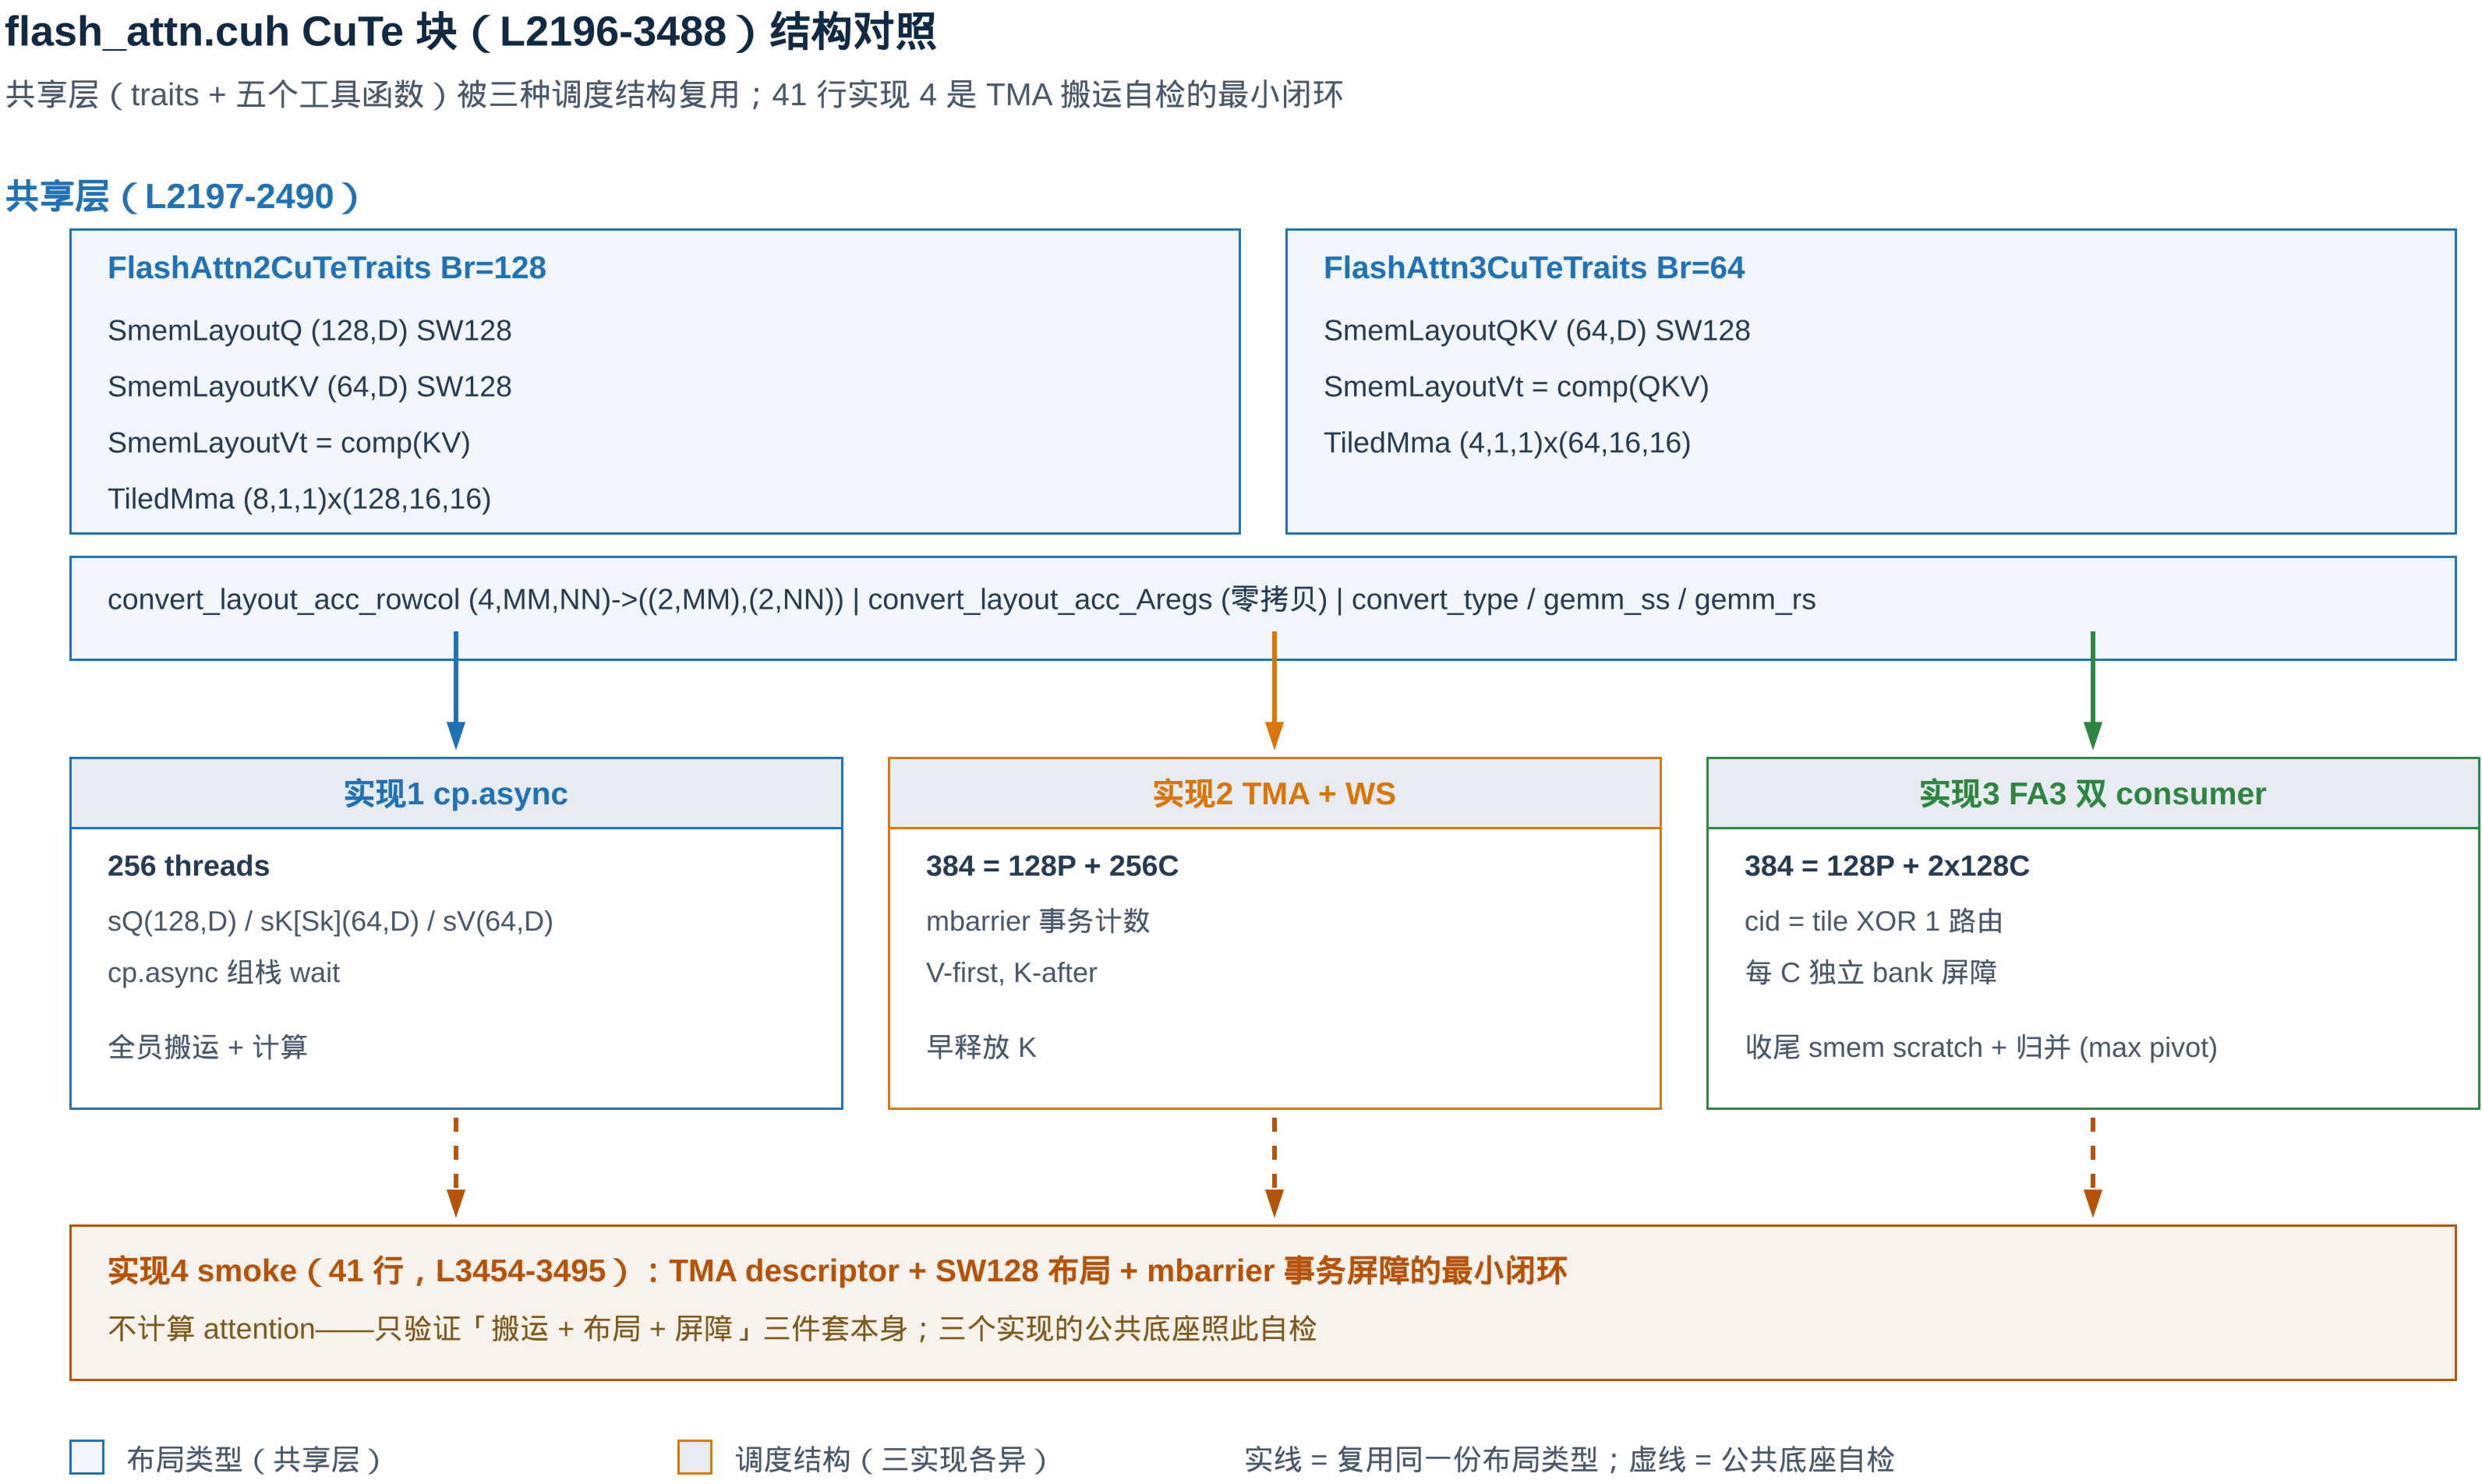
\includegraphics[width=0.98\textwidth]{figures/drawio/fig-25-1-cute-struct/fig-25-1.png}
\begin{tikzpicture}[font=\tiny, >=Stealth,
  secl/.style={font=\bfseries\fontsize{4.6}{5.2}\selectfont, inner sep=1pt},
  code/.style={font=\ttfamily\fontsize{4.2}{4.8}\selectfont, inner sep=1pt, anchor=west},
  sub/.style={font=\fontsize{4.2}{4.8}\selectfont, inner sep=1pt, anchor=west,
    align=left, text width=4.30cm},
  tcard/.style={draw=tkBlue, fill=tkFillBlue, inner sep=3pt},
  ihdr/.style={draw, fill=gray!14, align=center, inner sep=2pt,
    font=\bfseries\fontsize{4.4}{5}\selectfont},
]
  \node[secl, text=tkBlue, anchor=west] at (0,0.34) {共享层（L2197-2490）：traits + 五个工具函数};
  % 共享层：两个 traits 卡
  \draw[tcard] (0,-0.02) rectangle (7.00,-1.78);
  \node[code, text=tkBlue] at (0.10,-0.22) {\textbf{FlashAttn2CuTeTraits<D>}\ \ Br=128};
  \node[code] at (0.10,-0.56) {SmemLayoutQ\ \ (128,D)\ SW128};
  \node[code] at (0.10,-0.84) {SmemLayoutKV\ (64,D)\ SW128};
  \node[code] at (0.10,-1.12) {SmemLayoutVt\ = comp(KV)};
  \node[code] at (0.10,-1.40) {TiledMma\ \ (8,1,1)$\times$(128,16,16)};
  \draw[tcard] (7.50,-0.02) rectangle (14.50,-1.78);
  \node[code, text=tkBlue] at (7.60,-0.22) {\textbf{FlashAttn3CuTeTraits<D>}\ \ Br=64};
  \node[code] at (7.60,-0.56) {SmemLayoutQKV (64,D) SW128};
  \node[code] at (7.60,-0.84) {SmemLayoutVt\ = comp(QKV)};
  \node[code] at (7.60,-1.12) {TiledMma\ \ (4,1,1)$\times$(64,16,16)};
  % 共享层：工具函数横条
  \draw[tcard] (0,-1.95) rectangle (14.50,-2.55);
  \node[code] at (0.60,-2.25) {convert\_layout\_acc\_rowcol (4,MM,NN)$\to$((2,MM),(2,NN))};
  \draw[tkBlue!45, thin] (5.55,-2.00) -- (5.55,-2.50);
  \node[code] at (5.80,-2.25) {convert\_layout\_acc\_Aregs（零拷贝）};
  \draw[tkBlue!45, thin] (10.05,-2.00) -- (10.05,-2.50);
  \node[code] at (10.30,-2.25) {convert\_type\ /\ gemm\_ss\ /\ gemm\_rs};
  % 三个实现的调度结构卡（各自保持自己一层的调度色）
  \draw[draw=tkBlue, fill=white] (0,-3.00) rectangle (4.60,-5.00);
  \draw[draw=tkOrange, fill=white] (4.95,-3.00) rectangle (9.55,-5.00);
  \draw[draw=tkGreen, fill=white] (9.90,-3.00) rectangle (14.50,-5.00);
  \node[ihdr, text=tkBlue] at (2.30,-3.21) {实现 1：cp.async};
  \node[ihdr, text=tkOrange!85!black] at (7.25,-3.21) {实现 2：TMA + WS};
  \node[ihdr, text=tkGreen] at (12.20,-3.21) {实现 3：FA3 双 consumer};
  \node[sub] at (0.15,-3.66) {\textbf{256 threads}};
  \node[sub] at (0.15,-3.92) {sQ(128,D) / sK[$S_k$](64,D)};
  \node[sub] at (0.15,-4.18) {/ sV(64,D)};
  \node[sub] at (0.15,-4.44) {cp.async 组栈 wait<N>};
  \node[sub] at (0.15,-4.70) {全员搬运 $+$ 计算};
  \node[sub] at (5.10,-3.66) {\textbf{384 = 128P + 256C}};
  \node[sub] at (5.10,-3.92) {mbarrier 事务计数};
  \node[sub] at (5.10,-4.18) {V-first, K-after};
  \node[sub] at (5.10,-4.44) {早释放 K};
  \node[sub] at (10.05,-3.66) {\textbf{384 = 128P + 2$\times$128C}};
  \node[sub] at (10.05,-3.92) {cid = tile XOR 1 路由};
  \node[sub] at (10.05,-4.18) {每 C 独立 bank 屏障};
  \node[sub] at (10.05,-4.44) {收尾 smem scratch $+$ 归并};
  \node[sub] at (10.05,-4.70) {(max pivot)};
  % 共享层 -> 三实现（实线：复用同一份布局类型）
  \draw[->, tkBlue, semithick] (2.30,-2.60) -- (2.30,-2.96);
  \draw[->, tkOrange, semithick] (7.25,-2.60) -- (7.25,-2.96);
  \draw[->, tkGreen, semithick] (12.20,-2.60) -- (12.20,-2.96);
  % 实现 4：公共底座自检
  \node[draw=tkOrange!85!black, fill=tkFillOrange, align=center, inner sep=2pt,
    font=\fontsize{4.2}{4.8}\selectfont, text width=13.9cm]
    at (7.25,-5.80)
    {\textbf{实现 4 smoke（42 行，L3447-3488）：TMA descriptor $+$ SW128 布局 $+$ mbarrier 事务屏障的最小闭环}\\
     不计算 attention——只验证「搬运 $+$ 布局 $+$ 屏障」三件套本身；三个实现的公共底座照此自检};
  \draw[->, dashed, tkOrange, semithick] (2.30,-5.04) -- (2.30,-5.42);
  \draw[->, dashed, tkOrange, semithick] (7.25,-5.04) -- (7.25,-5.42);
  \draw[->, dashed, tkOrange, semithick] (12.20,-5.04) -- (12.20,-5.42);
  % 图例
  \fill[tkFillBlue, draw=tkBlue] (0.10,-6.60) rectangle (0.32,-6.82);
  \node[sub] at (0.42,-6.71) {布局类型（共享层复用）};
  \fill[gray!14, draw=tkOrange] (5.60,-6.60) rectangle (5.82,-6.82);
  \node[sub] at (5.92,-6.71) {调度结构（三实现各异）};
  \node[sub, text width=5.40cm] at (9.60,-6.71)
    {实线 $=$ 复用同一份布局类型；虚线 $=$ 公共底座自检};
\end{tikzpicture}
\caption{CuTe 块的四层结构：共享 traits 与五个工具函数（上），三个 attention
实现（中），以及 42 行的 TMA 搬运自检（底）。实线箭头表示同一份布局类型被
三种调度结构复用，虚线表示三个实现共用实现~4 的底座自检。}
\label{fig:25-1}
\end{figure}

\section{性能分析}

本节先交代源码注释里的既有数字与口径，再给本书的复测，最后汇总 CuTe 实测表。

先看源码注释。本章区间（L2196--3488）内\textbf{没有}任何 TFLOPS/加速比
断言：四个实现都是能跑对的对照样本，性能数字在相邻章节：
第~\ref{ch:16}~章区间内的 L61--71 注释给出 pad 与 XOR swizzle 的对照
（「约 120.0 TFLOPS，显著低于 Q/K/V kPad$=$8 的 166.6 TFLOPS」），
第~\ref{ch:17}~、\ref{ch:18}~章的性能节给出同机同批复测（RTX PRO 5000
sm\_120a、CUDA 13.2）。读这些数字时必须注意口径：$B{=}1,H{=}32$、
warmup$\ge$5、iters$\ge$20 取均值，FLOPS $=4BHN^2D$；
CuTe 版与手写版在\emph{同一口径}下才可比。

本书复测用的是本章测试（\texttt{book/\allowbreak{}tests/\allowbreak{}ch25\_\allowbreak{}fa\_\allowbreak{}cute.\allowbreak{}cu}），
\texttt{bench} 子命令按与第~\ref{ch:17}/\ref{ch:18}~章相同的口径测量
CuTe 实现 1/2 的吞吐：$B{=}1$、$H{=}32$、warmup$=5$、iters$=20$，
$D\in\{64,128\}$、$N\in\{4096\}$。三点预期：(1) 实现 1 与实现 2 的差异
是\textbf{搬运路径}（cp.async 全员搬 vs TMA 单线程发）而非计算，
$D{=}128$ 的 Q tile 更大（$128\times128$ 个 half $=32$\,KB），
实现 1 的 G2S 负载更重，两者差距应主要体现在大 $D$；
(2) 实现 3（双 consumer）与第~\ref{ch:18}~章手写 FA3 在 $B_r{=}64$ 上的
结构性差异只有谁搬，可对照式~\ref{eq:18-smem} 的 smem 占用；
(3) 本章全部实现是\textbf{非 causal、无 GQA/varlen} 的 self-attention，
与手写版限制相同（源码注释 L2528--2529 明示），因此这些数字只能说明
CuTe 化不牺牲性能，不能当作实现之间谁更快的定论。

CuTe 实测见表~\ref{tab:ch25-perf}：
\texttt{leetcuda\_\allowbreak{}bench\_\allowbreak{}sm120a.\allowbreak{}bin}
\texttt{--bench --bench-all} 的 FA CuTe 实测（RTX PRO 5000，sm\_120、110 SM、
CUDA 13.2；$B{=}1$、$H{=}32$、$N{=}8192$、$D{=}128$ dense，全部 F32Acc，
参照 cuDNN f32 的 230.2 TFLOPS）。

\begin{table}[H]
\centering
\caption{FA CuTe 实测（RTX PRO 5000，B=1 H=32 N=8192 D=128）}
\label{tab:ch25-perf}
\footnotesize
\setlength{\tabcolsep}{4pt}
\begin{tabular}{lrr}
\toprule
Kernel & Max Err & TFLOPS/cuDNN（加速比） \\
\midrule
FA2 CuTe MMA Stages (Sk=1, F32Acc) & 1.526e-05 & 184.4/230.2 (0.80x) \\
FA2 CuTe MMA Stages (Sk=2, F32Acc) & 1.526e-05 & 196.5/230.2 (0.85x) \\
FA2 CuTe TMA MMA WS (1 Consumer WG) (Sk=2, Sv=1, F32Acc) & 1.526e-05 & 218.6/230.2 (0.95x) \\
FA2 CuTe TMA MMA WS (1 Consumer WG) (Sk=3, Sv=1, F32Acc) & 1.526e-05 & 221.4/230.2 (0.96x) \\
\bottomrule
\end{tabular}
\end{table}

三个台阶清晰可见：实现 1 的 CuTe MMA Stages 已到 cuDNN 的 0.80--0.85$\times$，
纯 CuTe 抽象、无任何搬运特化就已接近厂商库；实现 2 的 CuTe TMA MMA WS 把
搬运与计算解耦后升到 0.95--0.96$\times$、逼近 cuDNN：TMA + warp
specialization 这条路线的收益在 CuTe 版上完整复现。再把 K 的 stage 从 2 加深到
3 只带来约 1.3\% 的提升（218.6 $\to$ 221.4 TFLOPS），流水深度的收益已边际递减；
更完整的 persistent-CTA WS 实现见第 26b 章。

\section{常见坑}

\textbf{坑一：K/V 的 \texttt{local\_tile} 坐标是打包维上的全局 tile 号。}
TMA tensor 的 shape 是 $[B\!\cdot\!H\!\cdot\!N, D]$，K/V 的块坐标必须写
\texttt{blockIdx.y * kv\_tiles + tile}；漏掉偏移时所有 head 读同一份 K/V：
$H{=}1$ 的正确性测试全绿，$H{>}1$ 的精度却差两个量级（源码 L2885--2892
的注释即为此事）。正确性测试必须包含 $H{\ge}2$（本章测试取 $H{=}2$）。

\textbf{坑二：\texttt{cp.\allowbreak{}async.\allowbreak{}wait\_\allowbreak{}group} 是 per-thread 的。}
它只保证\emph{本线程}提交的组完成；跨线程可见性仍要
\texttt{\_\allowbreak{}\_\allowbreak{}syncthreads\allowbreak{}()}。实现 1 里每一处 \texttt{wait} 后面都跟着一次
同步，不是冗余。省掉同步的版本可能在 $B_r{=}128$ 的负载下偶发错数据
（写入 smem 的线程与读取的线程不同）。

\textbf{坑三：V 是单 buffer，PV 之后必须同步才能进入下一轮。}
L2769 的 \texttt{\_\allowbreak{}\_\allowbreak{}syncthreads\allowbreak{}()} 注释写明「ldmatrix V 完成后才能覆盖
V smem」。删掉它，下一轮 3a 的 V cp.async 可能覆盖本轮尚未读完的 sV，
表现是间歇性数值错误，且只在 $D$ 大（ldmatrix 更多）时暴露。

\textbf{坑四：推导 B fragment 的寄存器布局时要用 nonswizzle 视图。}
\texttt{partition\_\allowbreak{}fragment\_\allowbreak{}B(sVt)} 若传入带 swizzle 的 \texttt{Smem\allowbreak{}Layout\allowbreak{}Vt}，
CuTe 推导 \texttt{ldmatrix.\allowbreak{}trans} 的线程-数据映射时会与 swizzle composition
冲突（源码 L2886--2893 与 L3010--3020 的两处注释）。正确做法是
\texttt{get\_\allowbreak{}nonswizzle\_\allowbreak{}portion}（寄存器布局与 smem 物理 swizzle 无关），
而 \texttt{partition\_S}（S2R copy 的源）仍用带 swizzle 的视图；两者
分工不能互换。

\textbf{坑五：\texttt{K} 的预取深度与尾部退化。}
$kStagesK>1$ 时 K 的预取位置是 \texttt{tile + kStagesK - 1}，尾部
$kStagesK{-}1$ 个 tile 不预取；此时栈里只剩 V 组，PV 前的 \texttt{wait<1>}
必须退化为 \texttt{wait<0>}（L2748--2753）。漏掉这个分支，尾部两个 tile
会等一个不存在的组，行为是等很久后照样算完（组计数不会变负），
但流水被拖成同步。

\textbf{坑六：\texttt{convert\_\allowbreak{}layout\_\allowbreak{}acc\_\allowbreak{}Aregs} 依赖 $m16n8k16$ 约定。}
式~\eqref{eq:25-aregs} 的 C 的后 2 值 $\leftrightarrow$ A 的 K 向连续 2 值
是 $m16n8k16$ 的 fragment 约定的推论，源码 L2360--2362 特意标注「不是通用
性质」。换 atom（如 $k8$ 或 wgmma）必须重推；照抄会得到静默错数据。

\textbf{坑七：P 的类型转换与布局重解释的先后顺序。}
正确顺序是 \texttt{convert\_\allowbreak{}type\allowbreak{}<Element>\allowbreak{}(t\allowbreak{}Cr\allowbreak{}S)} 再做
\texttt{convert\_\allowbreak{}layout\_\allowbreak{}acc\_\allowbreak{}Aregs}（实现 1 的 L2762--2766）：
\texttt{convert\_\allowbreak{}type} 用 \texttt{Numeric\allowbreak{}Array\allowbreak{}Converter} 按\emph{当前}
layout 的连续段做向量化转换，先改布局会让转换作用于错误的元素分组。

\textbf{坑八：f32 累加与 exp2 的缩放折叠。}
三处实现都写 \texttt{scale = rsqrtf(D) * M\_LOG2E}、用
\texttt{exp2f\allowbreak{}(s*scale - nxt)} 替代 \texttt{expf}：把 $1/\sqrt{D}$ 折进
$\log_2 e$ 既省一条乘法也让 SFU 走 \texttt{ex2.approx}。改动缩放因子时
必须同步改 \texttt{row\_\allowbreak{}max/\allowbreak{}\_\allowbreak{}sum} 的语义（它们都在 $\log_2$ 域），
否则 softmax 的归一化在数值上自洽但语义漂移。

\section{面试要点速查}

\textbf{Q1：CuTe 版 FlashAttention 消掉的到底是什么？}\\
A：消掉的是与调度正交的\emph{布局算术}：smem swizzle 的地址、ldmatrix 的
lane 映射、fragment 的寄存器编号、S$\to$P 的重解释。没有消掉的是
\emph{调度}：流水深度、屏障协议、释放时机（25.4.6 节）。CuTe 让 attention
变简单的准确说法是：简单在改 tile 不改正文，难的部分（等谁、何时释放）原样
保留。

\textbf{Q2：为什么 FA2 的 traits 用 8 个 warp、FA3 用 4 个？}\\
A：$B_r$ 不同（128 vs 64）。TiledMMA 的 AtomLayout 必须恰好铺满 $M$ 向
atom 数：$\langle16,8,16\rangle\otimes\langle8,1,1\rangle$ 的 $M$ 是 128，
$\langle4,1,1\rangle$ 的 $M$ 是 64。若 warp 数与 tile 不匹配，
\texttt{partition\_\allowbreak{}fragment\_\allowbreak{}C} 仍能编译，但会有 warp 拿到空 fragment
（静默低效）。

\textbf{Q3：\texttt{convert\_\allowbreak{}layout\_\allowbreak{}acc\_\allowbreak{}rowcol} 之后为什么是 4-lane 归约？}\\
A：$m16n8$ 的 C fragment 里，同一行的 2 个片段分布在 lane $\bmod 4$ 的
不同值上（式~\eqref{eq:25-rowcol-num} 的 $(2,1)$ 结构）；两次
\texttt{\_\allowbreak{}\_\allowbreak{}shfl\_\allowbreak{}xor\_\allowbreak{}sync}（步长 1、2）把宽度 4 的子组归约完，
再乘以每线程的列数即可。宽了会重复计数、窄了会漏行。

\textbf{Q4：P 为什么会零拷贝地变成 A 操作数？}\\
A：因为 $B_c$（S 的列）与 $PV$ 的 K 维是同一个物理维度，$m16n8k16$ 的
C 与 A 在该维度上的 2 元素的对应方式恰好兼容（式~\eqref{eq:25-aregs}）。
这是寄存器复用的经典技巧，CuTe 用一次 \texttt{logical\_\allowbreak{}divide} 表达，
代价是把它从技巧变成了有条件的等式，条件写在注释 L2360--2362。

\textbf{Q5：实现 2 的 V 为什么在 K 之前发 TMA？}\\
A：等待顺序是先 K 后 V（QK 需要 K、PV 需要 V），但\emph{发射}顺序是
V 先：V 的落盘窗口要横跨 QK+softmax 两段计算。这与实现 1 的
V 最后发、等 wait<1> 形异实同：都是让 V 的延迟藏在 softmax 里。

\textbf{Q6：四个实现里哪个最快？}\\
A：本章不做这个断言（25.6 节）：四者的 tile、线程、流水深度都不同，
受控对照需要在同一 $B_r/B_c/kStages$ 下比较。可确认的是：
CuTe 化没有牺牲吞吐（对照第~\ref{ch:17}/\ref{ch:18}~章复测）。

\textbf{Q7：TMA 的 mbarrier 协议里，phase 为什么每回绕一轮翻转？}\\
A：mbarrier 是相位对象而非计数器：arrive 数到零后相位翻转、
计数重置。stage 循环复用同一个 barrier 时，$t$ 号 tile 属于第
$\lfloor t/S\rfloor$ 个相位，故 phase $=$ 该商 $\bmod\ 2$
（图~\ref{fig:25-proto}）。写错 phase 的症状是等一个已经过去的相位：
永久挂起或提前通过。

\textbf{Q8：smoke kernel 为什么值得单独存在？（42 行）}\\
A：它是 TMA + SW128 布局 + 事务屏障三件套的最小闭环，把
\emph{搬运链路}与\emph{计算链路}解耦。调 attention 时先用它排除
搬运侧问题（descriptor 参数、box 与 layout 匹配、arrive\_tx 的字节数），
再去查计算侧；本章测试（25.9 节）的三个 case 全走实现 1，并未单独
驱动 smoke kernel；需要验搬运链路时可把它当独立小用例编译运行。

\section{最小测试与动手实验}

测试文件：\texttt{book/\allowbreak{}tests/\allowbreak{}ch25\_\allowbreak{}fa\_\allowbreak{}cute.\allowbreak{}cu}。三个 case 全部是
\textbf{端到端正确性}验证：固定 $B{=}1$、$H{=}2$、$k_{StagesK}{=}2$，全部
调用实现 1（cp.async 统一流水，256 线程），与 CPU fp64 参考
$\mathrm{softmax}(QK^\top/\sqrt{D})V$ 对照（half 输入/输出），容差
\texttt{TOL\_F16ACC}$=5\times10^{-2}$。形状约束：$N\bmod 128=0$
（$B_r{=}128$）且 $N\bmod 64=0$（$B_c{=}64$）、$D\in\{64,128\}$
（kernel 的 \texttt{static\_assert}；sm$_{80}+$）。三个形状的分工：

\begin{itemize}
  \item \textbf{case A（$D{=}64$，$N{=}128$）}：单 Q tile、KV 分 2 段，
        以最小形状走通完整的 online softmax KV 循环；
  \item \textbf{case B（$D{=}64$，$N{=}256$）}：多 Q tile，grid $(2,2)$
        （Q 方向 2 tile $\times$ $B{\cdot}H{=}2$），验证
        \texttt{local\_tile} 切分与 grid 映射；
  \item \textbf{case C（$D{=}128$，$N{=}128$）}：大 $D$ 路径，smem
        80\,KB $<$ 99\,KB optin，验证 traits 在 $D{=}128$ 下的 smem 预算
        与 fragment 形状。
\end{itemize}

host 端的 traits 结构断言（\texttt{tile\_\allowbreak{}size\_\allowbreak{}mnk}、fragment
形状、D-chunk 语义）与 TMA 往返 smoke 不在本测试内：前者由第~\ref{ch:22}~章
与第~\ref{ch:26}~章的最小测试承载，后者即本章实现 4 的 42 行 smoke kernel，
可单独编译驱动。

编译与运行（本机 sm\_120a，6 号卡；结果见下）：

{\footnotesize
\begin{lstlisting}[style=console]
$ cd book/tests && CUDA_VISIBLE_DEVICES=6 ./build_tests.sh --arch sm_120a --ch ch25
== ch25_fa_cute.cu (sm_120a)
PASS fa_cute cp.async D=64 Sk=2 B=1 H=2 N=128: max_abs_err=8.149e-05 (tol=5.0e-02)
PASS fa_cute cp.async D=64 Sk=2 B=1 H=2 N=256: max_abs_err=6.614e-05 (tol=5.0e-02)
PASS fa_cute cp.async D=128 Sk=2 B=1 H=2 N=128: max_abs_err=8.084e-05 (tol=5.0e-02)
ALL OK
\end{lstlisting}
}

动手实验建议：（1）把 case B 的 $H$ 改成 1、并把 kernel 换成实现 2
（需 \texttt{NOTES\_\allowbreak{}V2\_\allowbreak{}ENABLE\_\allowbreak{}TMA\_\allowbreak{}MMA\_\allowbreak{}WS}），再删掉实现 2 producer 的
\texttt{blockIdx.y * kv\_tiles} 偏移，正确性仍全绿，说明单 head
测试会掩蔽多 head 缺陷；（2）把实现 1 的模板参数从
\texttt{<64, 2>} 改成 \texttt{<64, 3>} 并打印 smem 用量，观察 K 三级时
smem 增量的构成（V 仍单 buffer）；（3）把 case A 的模板参数从
\texttt{<64, 2>} 改成 \texttt{<96, 2>}，观察 traits 的
\texttt{static\_\allowbreak{}assert\allowbreak{}(k\allowbreak{}Head\allowbreak{}Dim =\allowbreak{}=\allowbreak{} 64 || =\allowbreak{}=\allowbreak{} 128)} 拒绝编译，
再对照第~\ref{ch:26}~章 FFPA 的 \texttt{kHeadDim \% 64 == 0} 放宽条件；
（4）把实现 2 的 \texttt{kStagesK} 从 1 调到 2，核对 smem 是否仍在
sm\_120a 的 99\,KB optin 之内（$D{=}128$ 时 Q 一段就占 32\,KB）。



\section*{延伸阅读}

\begin{itemize}
  \item @竹熙佳处《写给大家看的 CuTe 教程：Layout Compose \& Inverse》\\
        \url{https://zhuanlan.zhihu.com/p/1962625273636845008}\\
        （$S\to P$ 布局变换的两种讲法：Tri Dao 的几何重排与 @reed 的
        inverse$\circ$compose 代数法，本章 25.3.4 节的主参考）；
  \item @reed《cute 之 简单 GEMM 实现》与《cute 之 高效 GEMM 实现》\\
        \url{https://zhuanlan.zhihu.com/p/667521327}\\
        \url{https://zhuanlan.zhihu.com/p/675308830}\\
        （Tensor $\to$ 分块 $\to$ 划分 $\to$ 拷贝 $\to$ 计算的组装范式、
        多级流水写法与 Epilogue 的来龙去脉；前者是本章实现 1 的蓝本，
        后者的四个高效是三级搭建的对照读物）；
  \item @竹熙佳处《写给大家看的 CuTe 教程：tiled mma》\\
        \url{https://zhuanlan.zhihu.com/p/1937145378446226159}\\
        （fragment 视角的 mma 线程-值映射，25.3.2--25.3.4 节的入门读物）；
  \item @66RING《使用 cutlass cute 复现 flash attention》\\
        \url{https://zhuanlan.zhihu.com/p/696323042}\\
        （CuTe 版 attention 的另一种组织：把 Q/K/V 的 smem 布局与 S2R copy
        全部交给 CuTe，25.3 节的类型推导链可与之互证）；
  \item @shengying.wei《FlashAttention 笔记：tiny-flash-attention 解读》\\
        \url{https://zhuanlan.zhihu.com/p/708867810}\\
        （极简 FA 实现里 MMA atom 与线程布局的选择逻辑，对应式~\eqref{eq:25-eurepeat}
        的另一种推导）；
  \item @Titus《GEMM 流水线：single/multi-stage、pipeline》\\
        \url{https://zhuanlan.zhihu.com/p/712451053}\\
        （软件流水的 stage 语义；25.3.5 节组栈 vs 事务计数两种等待模型的
        对照背景）；
  \item @竹熙佳处《写给大家看的 CuTe 教程：async pipeline》\\
        \url{https://zhuanlan.zhihu.com/p/2024832248386528275}\\
        （CuTe 里表达异步流水的最新手法，可与实现 1 的手写组栈用法并读）。
\end{itemize}

% ch26-cute-ffpa.tex — 撰写任务见 RFC.md F7
\chapter{CuTe 应用（三）：FFPA Split-D 的类型代数}\label{ch:26}

\section{本章导读}

第~\ref{ch:19}~章把 Split-D 当作\emph{算法}讲透了：为什么大 head\_dim 会触及
smem 容量上限、$S$ 如何沿 $D$ 切成 chunk、$O$ 如何拆成分量并在收尾合并、chunk 数与
流水级数的相位关系如何推导。本章换一个视角：把同一份代码（\texttt{ffpa\_\allowbreak{}attn.\allowbreak{}cuh}
的 CuTe 版）当作\emph{类型系统}来读，回答一个第~\ref{ch:19}~章刻意没有展开的问题：

\begin{quote}
  Split-D 的每一个结构决策（双 TiledMma、chunk 循环、独立 $O$ 累加器），
  在 CuTe 里究竟长什么\emph{类型}？哪些事实可以在 host 端离线断言，
  而不必等到 device 上跑出错误结果？
\end{quote}

这个视角有直接的工程收益。第~\ref{ch:25}~章已经演示过一次：手写 attention 里靠注释和
规则维持的 lane 映射、tile 计数、转置视图，在 CuTe 版里变成了
\texttt{print\allowbreak{}(layout)} 可以打印、\texttt{static\_\allowbreak{}assert} 可以断言、host 端
测试可以离线核对的\emph{类型事实}。FFPA 把这件事推得更远一步：Split-D 引入的
chunk 循环让归约维度被切开这件事也必须落在类型上：

\begin{itemize}[itemsep=2pt,topsep=2pt]
  \item QK 与 PV 用\emph{两个不同形状}的 TiledMma，却共享同一批 128 个线程；
        两个 fragment 为什么能免 smem 交接？
  \item $S$ 的归约维（$D$）被切成 $C$ 个 chunk，但 $S$ 的 fragment 形状
        \emph{一次都没有变}，chunk 循环到底切开了什么？
  \item 每个 chunk 一份 $O$ 累加器，$C\times 32$ 个 f32 逻辑累加值是怎么被
        类型推导出来的？
\end{itemize}

本章的叙述顺序与第~\ref{ch:25}~章一致：先给类型代数（26.3 节，所有公式都能
在 host 端用 CuTe 原语验证），再逐相位读 kernel（26.4 节），最后是常见坑、
面试速查与最小测试。全章沿一条数据流展开：Q/K 的 chunk 从 smem
切片进来、在 $S$ 的 32 个寄存器里跨 chunk 累加、经 rowcol 视图做 online
softmax 就地写回 $S$，再由 \texttt{convert\_type} 产生 f16 fragment、用 Aregs
重解释成 PV 的 A 操作数。每一步都只用
\emph{类型}回答数据在哪、什么形状、谁持有。两处布局变换（rowcol 与
Aregs）的通用讲法在第~\ref{ch:25}~章 25.3.4 节已经展开，本章只补 Split-D
语境下的增量。涉及算法推导（chunk 分解的数学、online softmax 的不变量、
相位计数）的地方，直接引用第~\ref{ch:19}~章，不重复。

前置：第~\ref{ch:19}~章（Split-D 算法）、第~\ref{ch:20}--\ref{ch:22}~章
（布局代数、TiledCopy、TiledMMA）、第~\ref{ch:25}~章（attention 的 CuTe 化，
包括共享层 \texttt{convert\_\allowbreak{}layout\_\allowbreak{}acc\_\allowbreak{}rowcol} 与 \texttt{convert\_\allowbreak{}layout\_\allowbreak{}acc\_\allowbreak{}Aregs}
的来历）。

\section{问题与动机}

Split-D 的动机在源头注释里写得很直白（\texttt{ffpa\_\allowbreak{}attn.\allowbreak{}cuh} L7--8）：
\textbf{支持 head\_dim $>128$ 的 large head-dim attention，通过 64-wide Split-D
chunks 处理}。第~\ref{ch:19}~章量化了为什么必须分：smem 容量、以及
$\mathrm{softmax}$ 的结构性位置。本节只关心分完之后抽象层多出的四个问题。

先从第~\ref{ch:25}~章的结论出发。FA2 的三个 CuTe 实现里，attention 的
$D$ 维（head\_dim）是\emph{一个整体}：Q/K/V 的 smem tile 直接是
$[B_r, D]$、$[B_c, D]$，TiledMma 的 $K$ 向一次覆盖 16 列，循环在 $N$（KV tile）
方向滚动。FFPA 把这两件事都改了：

\begin{enumerate}[itemsep=3pt,topsep=3pt]
  \item K 向（$D$）被切成 chunk，循环滚动。$D=512$ 时
        $C = 512/64 = 8$ 个 chunk；QK 的累加变成一个\emph{跨 chunk 的求和}，
        每个 chunk 内部仍是一条标准的 $k16$ MMA 链。
  \item QK 与 PV 的 TiledMma 形状不同。QK 要一次覆盖 $S[64,64]$
        （省掉 N-tile 循环），PV 每次只覆盖 $O$ 的 16 列，
        以缩小单次调用的 C fragment 与临时量；跨 chunk 的 $O$ 总量仍由
        $D$ 与线程数决定。两者共享同一批线程，$S$（QK 的 C fragment）必须
        变成 $P$（PV 的 A 操作数）。
  \item $O$ 的累加器按 chunk 分裂。$D=512$、$C=8$ 时，每个线程
        持有 $8\times32$ 个 f32 的 $O$ 分量。
  \item 生产者也要跟着分 chunk。TMA box 或 cp.async 的搬运单元
        从整块 $[64,D]$ 变成 $C$ 个 $[64,64]$。
\end{enumerate}

四个问题的共同点：它们\emph{都不是数值问题}（数值精度与归约顺序都已确
定），而是\textbf{类型与布局问题}：tile 怎么切、fragment 怎么换解释、寄存器
怎么编号、循环与 stage 怎么对应。把这四个问题逐个翻译成 CuTe 的类型与布局，
就是用 CuTe 抽象表达 Split-D 的全部内容。

本章引用的源码位置汇总在表~\ref{tab:26-code}。

\begin{table}[htbp]
\centering
\caption{本章引用的 \texttt{ffpa\_\allowbreak{}attn.\allowbreak{}cuh} 位置（CuTe 版，cp.async 路径
\texttt{ffpa\_\allowbreak{}split\_\allowbreak{}d\_\allowbreak{}cute}，L79--376）。TMA+WS 版在同构位置复用同一批
helper，差异归第~\ref{ch:19}~章。}
\label{tab:26-code}
\begin{tabular}{p{4.2cm}p{3.4cm}p{6.0cm}}
\toprule
源码位置 & 内容 & 本章视角 \\
\midrule
L42--61 & traits：smem 布局与双 TiledMma & 类型推导链（26.3.1） \\
L79--97 & kernel 签名与 chunk 常量 & 128 线程 / \texttt{kDChunks}（26.4.1） \\
L118--128 & G2S \texttt{TiledCopy} & TV 布局与 MMA 对齐（26.4.2） \\
L136--141 & V 的 fragment 布局预计算 & 转置视图与 nonswizzle（26.4.3） \\
L152--176 & fragment 尺寸与寄存器占用 & 可断言的常量（26.3.2） \\
L217--271 & Phase 1：QK 的 chunk 流水 & 归约维的循环表达（26.4.5） \\
L273--303 & Phase 2：softmax 与 $P$ 的生成 & rowcol 与 Aregs（26.3.3） \\
L307--353 & Phase 3：PV 的 chunk 循环 & 双 TiledMma 的交接（26.4.6） \\
L355--374 & Phase 4：归一化与写回 & 收尾的布局复用（26.4.7） \\
\bottomrule
\end{tabular}
\end{table}

\section{数学原理：类型与布局代数}

\subsection{两个 TiledMma 的推导链}

第~\ref{ch:22}~章给出了 TiledMMA 的三元组
$(\mathrm{Atom},\ \mathrm{AtomLayout},\ \mathrm{Tile})$，以及每线程补足的
atom 重复数（源码注释称之为 \texttt{EURepeat}）：

\begin{equation}
  \mathrm{EURepeat} \;=\; \frac{\mathrm{Tile}}
  {\mathrm{AtomShape}\otimes \mathrm{AtomLayout}} ,
  \qquad
  \mathrm{AtomShape} = (16,8,16),\quad \mathrm{AtomLayout} = (4,1,1).
  \label{eq:26-eurepeat}
\end{equation}

代入两个 Tile（\texttt{ffpa\_\allowbreak{}attn.\allowbreak{}cuh} L52--58）：

\begin{align}
  \text{QK:}\quad & (64,64,16) \oslash \bigl((16,8,16)\otimes(4,1,1)\bigr)
    = (64,64,16)\oslash(64,8,16) = \langle 1,8,1\rangle ,
  \label{eq:26-qk}\\[2pt]
  \text{PV:}\quad & (64,16,16) \oslash (64,8,16) = \langle 1,2,1\rangle .
  \label{eq:26-pv}
\end{align}

读法：$M$ 向的 4 个 atom 位置被 4 个 warp 分完（$\mathrm{AtomLayout}$ 的
$M$ 分量 $=4$，每 warp 负责 16 行，故 $M$ 向的重复数为 1）；$N$ 向没有
atom-layout 的分工（$N$ 分量 $=1$），所以 $N$ 向的重复数就是
$\mathrm{Tile}_N/8$：QK 是 8，PV 是 2。

\begin{quote}
  $\mathrm{EURepeat}_N$ 就是每个线程每个 k-step 发射的
  \texttt{mma.sync} 条数。\allowbreak{}QK 的 8 条一次覆盖 $S$ 的整个 64 列
  （$8\times n8$），于是 N-tile 循环整个消失；PV 的 2 条覆盖单次调用的
  16 列。一个完整 O chunk 为 64 列，chunk 内先由 4 个 N-tile 覆盖，
  外层 V-chunk 循环再遍历后续各个 64 列 chunk。
\end{quote}

图~\ref{fig:26-dual-mma} 把这条对比摆成两个 tile 网格：行维同样被
$\mathrm{AtomLayout}=(4,1,1)$ 的 4 个 warp 分完，列维的 atom 数相差 4 倍。

\begin{figure}[H]
\centering
\begin{tikzpicture}[
  blknum/.style={font=\footnotesize\bfseries, inner sep=1pt},
  axl/.style={font=\scriptsize, inner sep=1pt},
]
  % 行轴：4 warp 分 M=64（AtomLayout=(4,1,1) 的 M 分量 = 4，每 warp 16 行）
  \foreach \wr/\mlo/\mhi in {0/0/15, 1/16/31, 2/32/47, 3/48/63} {
    \node[axl,anchor=east,align=right] at (1.02,-\wr*0.86-0.43)
      {w\wr\\{\tiny $m\,\mlo..\mhi$}};
  }
  % 左网格：S = QK 的输出 tile 64x64（4 warp 行块 x 8 个 n8 atom 列块）
  \foreach \wr in {0,...,3} {
    \foreach \aa in {0,...,7} {
      \pgfmathtruncatemacro{\gra}{12+8*\aa}
      \pgfmathtruncatemacro{\mn}{\aa+1}
      \fill[tkBlue!\gra] (1.1+\aa*1.05,-\wr*0.86) rectangle (1.1+\aa*1.05+1.05,-\wr*0.86-0.86);
      \node[blknum] at (1.1+\aa*1.05+0.525,-\wr*0.86-0.43) {\mn};
    }
  }
  \draw[thick, tkBlue] (1.1,0) rectangle (9.5,-3.44);
  \foreach \wr in {1,2,3} {
    \draw[very thick] (1.1,-\wr*0.86) -- (9.5,-\wr*0.86);
  }
  \foreach \aa in {1,...,7} {
    \draw[thin] (1.1+\aa*1.05,0) -- (1.1+\aa*1.05,-3.44);
  }
  % 右网格：O 的单次 PV 调用视图 64x16（4 warp 行块 x 2 个 n8 atom 列块）
  \foreach \wr in {0,...,3} {
    \foreach \aa in {0,...,1} {
      \pgfmathtruncatemacro{\gra}{18+30*\aa}
      \pgfmathtruncatemacro{\mn}{\aa+1}
      \fill[tkGreen!\gra] (11.0+\aa*0.95,-\wr*0.86) rectangle (11.0+\aa*0.95+0.95,-\wr*0.86-0.86);
      \node[blknum] at (11.0+\aa*0.95+0.475,-\wr*0.86-0.43) {\mn};
    }
  }
  \draw[thick, tkGreen] (11.0,0) rectangle (12.9,-3.44);
  \foreach \wr in {1,2,3} {
    \draw[very thick] (11.0,-\wr*0.86) -- (12.9,-\wr*0.86);
  }
  \draw[thin] (11.95,0) -- (11.95,-3.44);
  % 顶部标题与 atom 刻度
  \node[font=\scriptsize\bfseries,align=center,text=tkBlue] at (5.3,0.85)
    {QK TiledMma：Tile $=(64,64,16)$\\$\mathrm{EURepeat}=\langle 1,8,1\rangle$};
  \node[font=\scriptsize\bfseries,align=center,text=tkGreen!70!black] at (11.95,0.85)
    {PV TiledMma：Tile $=(64,16,16)$\\$\mathrm{EURepeat}=\langle 1,2,1\rangle$};
  \node[axl,anchor=south,text=tkBlue] at (5.3,0.22) {$S$（每块 = 一个 $n8$ atom，格内数字 = 该 warp 本 k-step 发射的第几条 \texttt{mma.sync}）};
  \node[axl,anchor=south,text=tkGreen!70!black] at (11.95,0.22) {$O$ 的单次 PV 调用视图};
  \foreach \aa in {0,...,7} {
    \node[axl,anchor=north] at (1.1+\aa*1.05+0.525,-3.52) {\aa};
  }
  \foreach \aa in {0,...,1} {
    \node[axl,anchor=north] at (11.0+\aa*0.95+0.475,-3.52) {\aa};
  }
  \node[axl,anchor=north] at (5.3,-3.95) {atom 列序（$N$ 向，每块 8 列：QK 共 $8{\times}8{=}64$ 列）};
  \node[axl,anchor=north] at (11.95,-3.95) {单视图共 16 列};
  % 交接箭头
  \draw[-{Stealth},thick,tkPurple] (9.72,-1.72) -- (10.78,-1.72);
  \node[font=\scriptsize,anchor=south,text=tkPurple] at (10.25,-1.66) {$P$};
  \node[font=\tiny,align=center,anchor=north,text=tkPurple] at (10.25,-1.78) {softmax\\Aregs 交接};
  % 底部两行注记
  \node[axl,anchor=north west,align=left,text width=11.6cm] at (1.1,-4.35)
    {两个完整输出的 frag 相同：$\mathrm{frag}_S=\mathrm{frag}_O=((2,2),1,8)=32$ 值/线程
     （式~\eqref{eq:26-frag32}，第三 mode 的 8 来历不同）；右侧仅画 O chunk 的一个 N-tile，};
  \node[axl,anchor=north west,align=left,text width=11.6cm] at (1.1,-5.25)
    {差别全在 $N$ 向：\textcolor{tkBlue}{QK} 的 $\mathrm{EURepeat}_N{=}8$ ——8 条 \texttt{mma.sync} 一次覆盖 $S$ 整个 64 列，\textbf{N-tile 循环}消失；
     \textcolor{tkGreen!70!black}{PV} 的 $\mathrm{EURepeat}_N{=}2$ 覆盖单视图的 16 列，完整 O chunk 内需 4 个 N-tile，外层 V-chunk 再推进 64 列。};
\end{tikzpicture}
\caption{双 TiledMma 的 Tile 分工（式~\eqref{eq:26-qk}--\eqref{eq:26-pv}）。
左：QK 的输出 $S[64,64]$——4 个 warp 各占 16 行（$\mathrm{AtomLayout}$ 的 $M$ 分量 4），
列向 8 个 $n8$ atom 由\textbf{同一线程}在一个 k-step 里连发 8 条 \texttt{mma.sync} 覆盖
（蓝深浅 8 档标识 atom 身份，格内数字为发射序）；右：PV 单次调用的输出视图为
$[64,16]$（绿 2 档、2 个 atom、2 条 \texttt{mma.sync}），完整 O chunk 为 $[64,64]$，
由 4 个这样的 N-tile 组成。中间箭头是 26.3.3 节的
交接：$S$ 经 softmax 后由 \texttt{convert\_type} 转成 f16 fragment，
\texttt{Aregs} 再重解释其布局作为 PV 的 A 操作数；全程不经过 smem。}
\label{fig:26-dual-mma}
\end{figure}

对照第~\ref{ch:25}~章 FA2 traits 的 $(8,1,1)\otimes(128,16,16)$：那里是
8 个 warp 分 $M=128$，$N$ 向重复数为 2。同一套公式，两种分工：FA2 把线程
堆在 $M$ 上换取更大的 $B_r$；FFPA 仍是 4 个 warp 分 $M=64$，$N$ 向没有
atom-layout 分工，一次覆盖整行块 $S$ 靠的是同一线程的
$\mathrm{EURepeat}_N=8$，不是把线程堆到 $N$ 上。

\subsection{fragment 的元素计数：两个恒等式}

TiledMma 定下来之后，每个线程持有多少寄存器就定了。这里有两个恒等式，后面
要讲的免 smem 交接就建立在它们上。

\textbf{恒等式一（C fragment 的大小）}：
\texttt{partition\_\allowbreak{}fragment\_\allowbreak{}C} 把\emph{目标输出形状}按 TiledMma 的线程布局
切开，所以

\begin{equation}
  \bigl|\mathrm{frag}_C\bigr| \;=\;
  \frac{\bigl|\text{目标输出形状}\bigr|}{\text{线程数}} .
  \label{eq:26-csize}
\end{equation}

FFPA 的两处调用（L152 与 L218）目标形状都是 $(64,64)$，线程数都是 128，
所以 QK 的 $S$ 与 PV 的 $O$ 都是每线程 32 个 f32。实测：

\begin{equation}
  \mathrm{frag}_S = \bigl((2,2),1,8\bigr) = 32\ \text{值/tid},\qquad
  \mathrm{frag}_O = \bigl((2,2),1,8\bigr) = 32\ \text{值/tid} .
  \label{eq:26-frag32}
\end{equation}

注意 $\mathrm{frag}$ 的第三 mode 是 8：那是 QK 的 $\mathrm{EURepeat}_N$
在 $S$ 上的投影。$O$ 的第三 mode 数字恰好也是 8，但它来自目标输出
$64$ 列按每个 $n8$ atom 分出的 $8$ 个列组（$64/8{=}8$），
不是 $\mathrm{EURepeat}_N$ 的 $8$。两个 32 的来历不同、大小相同，
这是 $S\to P$ 与 $P\to O$ 两条交接链路能成立的前提。

恒等式二（rowcol 视图的行列数）：online softmax 要在
行上做 max/sum，所以第~\ref{ch:25}~章的工具函数
\texttt{convert\_\allowbreak{}layout\_\allowbreak{}acc\_\allowbreak{}rowcol} 把 $C$ fragment 从
$(\mathrm{MMA}=4,\ \mathrm{MMA\_M},\ \mathrm{MMA\_N})$ 重排成
$\bigl((2,\mathrm{MMA\_M}), (2,\mathrm{MMA\_N})\bigr)$。FFPA 用它推两个
常量（L158--162）：

\begin{equation}
  \mathrm{nrow} = 2\cdot\mathrm{MMA\_M} = 2, \qquad
  \mathrm{ncol} = 2\cdot\mathrm{MMA\_N} = 16 .
  \label{eq:26-rowcol}
\end{equation}

$\mathrm{nrow}=2$ 的含义：\emph{每个线程只拥有 2 行}，行内 16 列。
$n16$ 的 $C$ fragment 里，一个线程的 4 个值的一半（行偏移 $+8$ 的那对）
属于另一行；4 个线程（lane 的 $\text{id}/4$ 相同、$\text{id}\bmod 4$ 不同）
拼成完整的一行，源码里行归约只用 \texttt{\_\allowbreak{}\_\allowbreak{}shfl\_\allowbreak{}xor\_\allowbreak{}sync} 掩码 1 与 2
（后者把 4 个 lane 的两两组合并），原因就在这里。第~\ref{ch:25}~章在手写版
同步链里数过的谁和谁在同一行，在 FFPA 里被压缩成两个常量。

\subsection{$S \to P$：免 smem 的布局重解释}

$S$（QK 的 C fragment，f32）要变成 PV 的 A 操作数 $P$（f16）。两步操作
（L301--303）：

\begin{enumerate}[itemsep=2pt,topsep=2pt]
  \item \texttt{convert\_\allowbreak{}type\allowbreak{}<Element>\allowbreak{}(t\allowbreak{}Cr\allowbreak{}S)}：用
        \texttt{NumericArrayConverter} 做 f32$\to$f16 数值转换，并产生新的
        f16 fragment；它只作用于底层平坦数组，不按当前 layout 的连续段分组。
  \item \texttt{convert\_\allowbreak{}layout\_\allowbreak{}acc\_\allowbreak{}Aregs\allowbreak{}<Tiled\allowbreak{}Mma\allowbreak{}PV>\allowbreak{}(layout)}：把布局
        重解释成 $m16n8k16$ 的 A 操作数布局；这一步不搬动底层数组。
\end{enumerate}

源码先做类型转换、再做 Aregs；但两者不是按 layout 连续段绑定的。转换器只
看到底层平坦数组，Aregs 只重解释索引，所以不能把“反序会按错误连续段分组”
当作顺序理由。Aregs 本身调用的就是第~\ref{ch:25}~章 25.3.4 节精读过的那个
\texttt{convert\_\allowbreak{}layout\_\allowbreak{}acc\_\allowbreak{}Aregs}
（Tri Dao 的 \texttt{logical\_\allowbreak{}divide} 几何法与 @reed 的
inverse$\circ$compose 代数法都在讲同一件事）。放到 Split-D 的语境里，
补三点增量：

\begin{itemize}[itemsep=2pt,topsep=2pt]
  \item \textbf{为什么免 smem 往返}：$S$ 的 32 个寄存器是 Phase 2 最紧张
        的资源，softmax 之后直接转换成 $P$；若改走 $P$ 写回 smem 再
        ldmatrix，每个 kv\_tile 在完整 QK 与 softmax 之后会多出一次
        $64\times64$ 的 half 往返与一次同步。这笔开销按 kv\_tile 数计，
        不随 D-chunk 数 $C$ 成倍增加。
  \item \textbf{为什么模板参数是 \texttt{\allowbreak{}<Tiled\allowbreak{}Mma\allowbreak{}PV>}}：Aregs 重解释要按
        \emph{消费者}的 atom 约定推：PV 的 $k16$ atom 决定 K 向 2 值
        落在哪个寄存器编号上，而不是 QK 的约定。
  \item \textbf{数据流本身}：$S$ 的列（$B_c$ 向）在 $P$ 里变成 K 向，而
        $PV$ 的归约恰好沿这个方向；$P$ 的生产者（softmax）与消费者（PV）
        作用在同一维上，变换只调整哪个寄存器读哪一对列。
\end{itemize}

第二步为什么合法？在 atom 一级看两个 fragment 的\emph{线程-值}映射
（第~\ref{ch:22}~章符号；$m$ 行、$k$ 是 $P$ 的 K 向 $=S$ 的列）：

\begin{align}
  C\ (m16n8):\quad & m = \frac{lane}{4} + 8d_1,\quad
    n = 2\,(lane\bmod 4) + d_0, \qquad v = d_0 + 2d_1, \label{eq:26-cmap}\\
  A\ (m16k16):\quad & m = \frac{lane}{4} + 8d_1,\quad
    k = 2\,(lane\bmod 4) + d_0 + 8d_2, \qquad v = d_0 + 2d_1 + 4d_2 .
  \label{eq:26-amap}
\end{align}

把式~\eqref{eq:26-cmap} 的 $C$ 映射沿值方向拆位：低 2 个值（$v=0,1$，即 $(d_0,d_1)=(0,0),(1,0)$）
是\emph{同一行、相邻两列}（$d_0$ 即列 $+1$）；高 2 个值（$d_1=1$）是
行 $+8$ 的另一对。而式~\eqref{eq:26-amap}
的 $A$ 映射里，$d_0$ 同样是 k 向相邻 2 值。于是 C 的 4 个值与
A 的 4 个值在寄存器里一一对应：A 的 $k$ 向 2 值 $=$ C 的
列向 2 值，A 的行维与 C 的行维本来就一致。第~\ref{ch:25}~章把这条性质
记作\textbf{不是通用性质，换 atom 必须重推}（源码 L2360 附近的注释）；在 FFPA
里它的意义更重：$P$ 的 K 向就是 $S$ 的列向，而那一维正是 PV 的
归约维，重解释的方向恰好对齐 MMA 的约定，所以不需要 shuffle、
不需要过 smem。

图~\ref{fig:26-camap} 把这两条映射放到同一批格子上逐位核对：
同一个 lane 在两图里高亮的位置完全相同，变的只是值编号与分组。

\begin{figure}[H]
\centering
\begin{tikzpicture}[
  cfl/.style={font=\tiny, inner sep=0.2pt},
  axl/.style={font=\scriptsize, inner sep=1pt},
  nt/.style={font=\scriptsize, align=left, inner sep=1.5pt},
]
  % 左：C 视图 m16 x 16（两个 n8 atom 拼成）；高亮 lane 6 的 8 个值
  \foreach \rr in {0,...,15} {
    \foreach \cc in {0,...,15} {
      \pgfmathtruncatemacro{\hit}{(\rr==1 || \rr==9) && (\cc==4 || \cc==5 || \cc==12 || \cc==13) ? 1 : 0}
      \ifnum\hit=1
        \fill[colorx6!45] (\cc*0.42,-\rr*0.42) rectangle (\cc*0.42+0.41,-\rr*0.42-0.41);
        \draw[thick,colorx6!75!black] (\cc*0.42,-\rr*0.42) rectangle (\cc*0.42+0.41,-\rr*0.42-0.41);
      \else
        \filldraw[fill=gray!22, draw=gray!55, thin] (\cc*0.42,-\rr*0.42) rectangle (\cc*0.42+0.41,-\rr*0.42-0.41);
      \fi
    }
  }
  \foreach \rr/\cc/\vv in {1/4/0, 1/5/1, 9/4/2, 9/5/3, 1/12/0, 1/13/1, 9/12/2, 9/13/3} {
    \node[cfl,font=\tiny\bfseries] at (\cc*0.42+0.205,-\rr*0.42-0.205) {\vv};
  }
  \draw[thick] (0,0) rectangle (6.72,-6.72);
  \draw[very thick] (3.36,0) -- (3.36,-6.72);
  \foreach \rx in {0,4,8,12,15} {
    \pgfmathsetmacro{\ry}{-\rx*0.42-0.21}
    \node[axl,anchor=east] at (-0.1,\ry) {\rx};
  }
  \node[axl,anchor=south,rotate=90] at (-0.66,-3.36) {行 $m$};
  \node[axl,anchor=north] at (1.68,-6.85) {$n8$ atom 0};
  \node[axl,anchor=north] at (5.04,-6.85) {$n8$ atom 1};
  \node[axl,anchor=north] at (3.36,-7.35) {C 视图：列 $n$（$S$ 的 $B_c$ 向）};
  % 中间：同一批寄存器
  \node[axl,rotate=90] at (7.66,-3.36) {同一批 f16 寄存器，换 A 的约定读（布局重解释）};
  % 右：A 视图 m16 x 16（一个 k16 atom）
  \foreach \rr in {0,...,15} {
    \foreach \cc in {0,...,15} {
      \pgfmathtruncatemacro{\hit}{(\rr==1 || \rr==9) && (\cc==4 || \cc==5 || \cc==12 || \cc==13) ? 1 : 0}
      \ifnum\hit=1
        \fill[colorx6!45] (\cc*0.42+8.6,-\rr*0.42) rectangle (\cc*0.42+9.01,-\rr*0.42-0.41);
        \draw[thick,colorx6!75!black] (\cc*0.42+8.6,-\rr*0.42) rectangle (\cc*0.42+9.01,-\rr*0.42-0.41);
      \else
        \filldraw[fill=gray!22, draw=gray!55, thin] (\cc*0.42+8.6,-\rr*0.42) rectangle (\cc*0.42+9.01,-\rr*0.42-0.41);
      \fi
    }
  }
  \foreach \rr/\cc/\vv in {1/4/0, 1/5/1, 9/4/2, 9/5/3, 1/12/4, 1/13/5, 9/12/6, 9/13/7} {
    \node[cfl,font=\tiny\bfseries] at (\cc*0.42+8.805,-\rr*0.42-0.205) {\vv};
  }
  \draw[thick] (8.6,0) rectangle (15.32,-6.72);
  \draw[dashed,very thick] (11.96,0) -- (11.96,-6.72);
  \foreach \rx in {0,4,8,12,15} {
    \pgfmathsetmacro{\ry}{-\rx*0.42-0.21}
    \node[axl,anchor=east] at (8.5,\ry) {\rx};
  }
  \node[axl,anchor=south,rotate=90] at (7.94,-3.36) {行 $m$};
  \node[axl,anchor=north] at (10.28,-6.85) {$d_2{=}0$};
  \node[axl,anchor=north] at (13.64,-6.85) {$d_2{=}1$};
  \node[axl,anchor=north] at (11.96,-7.35) {A 视图：K 向 $k$（$PV$ 归约维，一个 $k16$ atom）};
  % 底部：两条映射式
  \node[nt,anchor=north west,text width=15.6cm] at (0,-7.65)
    {C（$m16n8$）：$m=\frac{lane}{4}+8d_1$、$n=2\,(lane\bmod4)+d_0$、$v=d_0+2d_1$；
     A（$m16k16$）：$m$ 同式、$k=2\,(lane\bmod4)+d_0+8d_2$、$v=d_0+2d_1+4d_2$
     （式~\eqref{eq:26-cmap}/\eqref{eq:26-amap}）。示例 lane$=6$：两图高亮的 8 格位置逐格相同
     （$m\in\{1,9\}$、列 $\{4,5\}\cup\{12,13\}$），C 的值编号在两个 atom 内各自 $0..3$ 循环，
     A 因多出 $d_2$ 而连续成 $0..7$——\textbf{A 的 K 向 2 值 $=$ C 的列向 2 值，行维本来就一致}。};
\end{tikzpicture}
\caption{C 与 A fragment 的线程-值映射逐位对照（式~\eqref{eq:26-cmap}/\eqref{eq:26-amap}）。
左：$S$ 的 C 视图——两个 $n8$ atom 拼成 16 列，格内数字是 lane 6 所持值的编号
$v=d_0+2d_1$（在每个 atom 内循环 $0..3$）；右：$P$ 的 A 视图——同一个 $k16$ atom，
lane 6 持有同样的 8 个格，值编号变成 $v=d_0+2d_1+4d_2$ 连续 $0..7$，其中
$d_2{=}1$ 的 4 格来自 C 的第二个 $n8$ atom（虚线半块）。\textbf{两图高亮位置逐格相同、
数据指针不换}：重解释只把\textbf{列向相邻 2 值}的约定换成\textbf{K 向相邻 2 值}，
行维（$m$）的映射本来就一致。}
\label{fig:26-camap}
\end{figure}

\begin{remark}
  如果 PV 的 atom 换成 SM80 的 $k8$，A 的 K 向只剩 8 列，$S$ 的 16 列要拆成
  两次 PV。但该 atom 的 A 与 C 都使用 \texttt{SM80\_16x8\_Row}，线程--值映射
  相同，所以每次 $k8$ PV 仍可复用布局，不能仅凭少了 $d_2$ 就断言零拷贝失效。
  换成 wgmma 等其他操作数约定时才需另推。第~\ref{ch:19}~章讨论过的
  \textbf{QK 与 PV 能不能共用一份 $P$}，判据是目标 atom 的 A/C 映射是否兼容。
\end{remark}

\subsection{D-chunk 循环的布局语义}

最后一个代数问题是 chunk 循环切开了什么。先给结论：

\begin{quote}
  Split-D 不改变任何 fragment 的形状，它改变的是\emph{循环结构}和
  \emph{归约树}。
\end{quote}

看 $S$ 的归约：$S = QK^{\top}$ 的真形式是 $S_{ij} = \sum_{d=0}^{D-1}Q_{id}K_{jd}$。
数值上它是一条长 $K$ 向链；结构上 FFPA 把它组织成两级：

\begin{equation}
  S_{ij} \;=\; \sum_{c=0}^{C-1}\ \underbrace{\sum_{t=0}^{3}\sum_{s=0}^{15}
  Q_{i,\,64c+16t+s}\,K_{j,\,64c+16t+s}}_{\text{chunk } c\ \text{内部：4 个 } k16\ \text{atom}} ,
  \qquad C = \frac{kHeadDim}{64} .
  \label{eq:26-splitd}
\end{equation}

式~\eqref{eq:26-splitd} 的两级结构在代码里对应两种不同的机制：

\begin{itemize}[itemsep=2pt,topsep=2pt]
  \item \textbf{chunk 内部}：\texttt{gemm\_ss} 的 K 循环（第~\ref{ch:25}~章
        共享层函数），循环上界来自 A fragment 的布局
        $\mathrm{size}<2>(\mathrm{frag}_A)=4$，即\emph{布局决定循环次数}。
  \item \textbf{chunk 之间}：\texttt{tCrS} 在 chunk 循环外声明、循环内\emph{累加}
        （L218 与 L237--270），归约体现为同一个寄存器数组跨迭代存活。
\end{itemize}

第二点的意义：$S$ 的 fragment 从头到尾是 32 个寄存器，chunk 循环每轮往
它们里面\emph{加}一棵 QK 子树，形状不变、只叠循环。$O$ 的处理不同，但不是
把各 $O_c$ 相加：$O$ 的 D 维被切成互不相交的列块，每个 $O_c$ 只对应其中
一块输出列；Phase 4 对每个分量独立归一化，再写回该列块。$S$ 的 chunk 是
\emph{归约维上的部分和}，必须先求和再做完整 softmax；$O$ 的 chunk 是
\emph{输出维上的分块}，各块保留同一行的 softmax 统计量。第~\ref{ch:19}~章
从数值角度论证过这一点，这里从类型角度再确认：$S$ 是一个 fragment 多次
迭代，$O$ 是多个 fragment 各存一份，代码形状（\texttt{tCrS} vs
\texttt{o\_\allowbreak{}acc\_\allowbreak{}storage[v]}）如实反映了这一点。
图~\ref{fig:26-splitd-struct} 把两者画成“归约树”与“输出列块树”的对比：
左边全部 chunk 汇进同一批 32 寄存器，右边每个 chunk 各占一份存储并写到
不同的 D 列块。

\begin{figure}[H]
\centering
\begin{tikzpicture}[
  axl/.style={font=\scriptsize, inner sep=1pt},
  tnb/.style={font=\tiny, inner sep=0.5pt},
]
  % 顶部：D 维横条，8 个 64-wide chunk（灰度 8 档），每 chunk 4 个 k16 子块
  \node[axl,anchor=east,align=right] at (0.92,-0.28) {Q/K 的\\$D$ 维};
  \node[axl,anchor=south] at (7.0,0.06)
    {$D=512\ \to\ C=8$ 个 64-wide chunk，每 chunk 内 4 个 $k16$ atom（式~\eqref{eq:26-splitd}）};
  \foreach \cc in {0,...,7} {
    \pgfmathtruncatemacro{\gra}{12+8*\cc}
    \fill[gray!\gra] (1.0+1.5*\cc,0) rectangle (2.5+1.5*\cc,-0.55);
    \foreach \ss in {1,2,3} {
      \draw[thin] (1.0+1.5*\cc+0.375*\ss,0) -- (1.0+1.5*\cc+0.375*\ss,-0.55);
    }
    \ifnum\gra>46
      \node[tnb,white] at (1.75+1.5*\cc,-0.28) {c\cc};
    \else
      \node[tnb] at (1.75+1.5*\cc,-0.28) {c\cc};
    \fi
  }
  \draw[thick] (1.0,0) rectangle (13.0,-0.55);
  % Phase 标签
  \node[axl,anchor=west] at (1.0,-0.95) {\textbf{Phase 1（QK）：$S$ 的跨 chunk 累加}};
  \node[axl,anchor=west] at (7.3,-0.95) {\textbf{Phase 3（PV）：$O$ 的分 chunk 存储}};
  % 左 panel：8 棵 qk 子树汇入单个 S fragment
  \foreach \cc in {0,...,7} {
    \pgfmathtruncatemacro{\gra}{12+8*\cc}
    \fill[gray!\gra] (1.0+0.7*\cc,-1.4) rectangle (1.6+0.7*\cc,-1.78);
    \node[tnb] at (1.3+0.7*\cc,-1.59) {$qk_{\cc}$};
    \pgfmathtruncatemacro{\gln}{0.6*\gra}
    \draw[-{Stealth},gray!\gln!black,thick] (1.3+0.7*\cc,-1.78) -- (1.3+0.7*\cc,-2.42);
  }
  \node[axl,anchor=west] at (1.0,-1.12) {\tiny 同一批 32 寄存器反复被加：};
  \draw[very thick,tkBlue,fill=tkFillBlue] (1.0,-2.42) rectangle (6.6,-3.32);
  \node[axl] at (3.8,-2.72) {$\mathtt{tCrS}$：32 f32/线程};
  \node[axl] at (3.8,-3.08) {\tiny 跨迭代存活 $\cdot$ 先求和、再 softmax};
  % 右 panel：8 份独立 fragment，Phase 4 逐块归一化写回
  \foreach \cc in {0,...,7} {
    \pgfmathtruncatemacro{\gra}{12+8*\cc}
    \pgfmathsetmacro{\yy}{-1.4-0.34*\cc}
    \fill[gray!\gra] (7.3,\yy) rectangle (7.62,\yy-0.28);
    \pgfmathtruncatemacro{\gfo}{0.4*\gra}
    \pgfmathtruncatemacro{\gln}{0.6*\gra}
    \foreach \gg in {0,...,7} {
      \draw[thin,fill=gray!\gfo] (7.66+0.3*\gg,\yy) rectangle (7.96+0.3*\gg,\yy-0.28);
    }
    \node[tnb,anchor=west] at (7.99,\yy-0.14) {$O_{\cc}$：32 f32/线程};
    \draw[-{Stealth},gray!\gln!black] (10.6,\yy-0.14) -- (11.25,\yy-0.14);
  }
  \node[axl,anchor=west] at (7.3,-1.12) {\tiny \texttt{o\_acc\_storage[c][32]}，各分量独立 rescale：};
  \draw[thick] (7.3,-1.4) rectangle (10.6,-4.12);
  \node[font=\large] at (11.55,-2.6) {逐块};
  \draw[-{Stealth},thick,tkGreen] (11.85,-2.6) -- (12.35,-2.6);
  \draw[very thick,tkGreen,fill=tkFillGreen] (12.35,-2.95) rectangle (14.15,-2.25);
  \node[axl,align=center] at (13.25,-2.6) {Phase 4\\归一化 + 写回};
  % 底部注记与对比标语
  \node[axl,anchor=north west] at (1.0,-3.45)
    {\tiny softmax 必须在\textbf{完整}的 $S$ 上做（第~\ref{ch:19}~章的数值论证）};
  \node[axl,anchor=north west] at (1.0,-3.85)
    {\tiny $S$ 的归约 = 加法进同一批寄存器；$O$ = 输出 D 列块各自归一化写回};
  \node[axl,anchor=north west,align=left,text width=6.1cm] at (7.3,-4.4)
    {\tiny $D{=}512$ 时 $8\times32=256$ 个 f32 逻辑值，已超过每线程 255 个寄存器的上限（见 26.5 节）};
  \node[font=\scriptsize\bfseries,anchor=west] at (1.0,-5.3)
    {对比：$S$ 先沿归约维求和再 softmax $\;\Vert\;$ $O$ 分 D 列块独立写回};
\end{tikzpicture}
\caption{Split-D 改变的是循环结构与归约树，不是 fragment 形状（26.3.4 节）。
顶条：$D=512$ 切成 $C=8$ 个 64-wide chunk（灰度 8 档贯穿全图），每 chunk 内
4 个 $k16$ atom 对应 \texttt{gemm\_ss} 的 K 循环。左：8 棵 QK 子树全部加进
\textbf{同一个} \texttt{tCrS} fragment——\textbf{一个 fragment 多次迭代}，softmax 必须等
求和完成；右：每个 chunk 的 PV 结果各存一份 \texttt{o\_acc\_storage[c][32]}，
对应输出 D 维上不同的 64 列块。Phase 4 对每块独立归一化并写回自己的列块，
不做 $O=\sum_c O_c$。$S$ 与 $O$ 的 32 值/线程形状完全相同，差别在
$S$ 沿归约维跨迭代累加，$O$ 沿输出维分块保存。}
\label{fig:26-splitd-struct}
\end{figure}

最后是 stage 与 chunk 的正交性。chunk 数 $C$ 由 head\_dim 决定，stage 数
$\mathrm{Sk}/\mathrm{Sv}$ 由 smem 预算决定，两者独立。当前源码选择用
\emph{指针算术}表达 stage 池：

\begin{equation}
  \texttt{q\_base} + \texttt{stage}\times \texttt{k\allowbreak{}QChunk\allowbreak{}Elements},
  \qquad
  \texttt{k\allowbreak{}QChunk\allowbreak{}Elements} = \mathrm{cosize}(\mathrm{SmemLayoutQ}) .
  \label{eq:26-stage}
\end{equation}

这是实现选择，不是 CuTe 布局代数的唯一写法。若要在类型里表达真实 stage
池，可以使用 stride 等于 \texttt{kQChunkElements} 的 stage mode；每个 stage
对应池中一块互不重叠的存储。只有把 stage 做成 stride-0 的伪维时才不同：
那表示所有 stage 落到同一元素，\texttt{cosize} 和 partition 的结果自然
不再对应池大小。FFPA 这里把布局限制为单块 chunk，把池偏移留在指针上，
是为了让每个轮转视图的类型保持最简单。

那么切片与流水在代码里具体长什么样？看 QK 主循环（L237--266）：
gmem 侧的 chunk 由 \texttt{local\_tile} 切出（坐标是 $(q\_tile, d\_chunk)$，
$d$ 从 $0$ 滚到 $\mathrm{Sk}{-}1$）；smem 侧每轮把 \texttt{q\_base} 加上
环状槽位偏移 \texttt{qk\_read} $\times$ \texttt{k\allowbreak{}QChunk\allowbreak{}Elements}，重新
包成一个 \texttt{SmemLayoutQ} 的 tensor。类型是常量、指针是变量：每轮更换的
只是槽位基址，tensor 的布局不变。随后 \texttt{partition\_\allowbreak{}fragment\_\allowbreak{}A} 与
\texttt{s2r\_thr\_q} 的 \texttt{partition\_S} 在这个只描述一块 chunk 的视图
上照常工作（两者的参数都是 \texttt{sQ\_stg}）。

对照第~\ref{ch:25}~章的三级搭建，那里 smem 是常驻的几段静态视图，这里换成了
按 stage 轮转的池：对 CuTe 而言两者没有区别，都是带 layout 的 tensor。流水
的推进则是 \texttt{qk\_read}/\texttt{qk\_write} 两个模 $\mathrm{Sk}$ 的计数器加
\texttt{cp\_\allowbreak{}async\_\allowbreak{}wait\allowbreak{}<Sk-2>}，与第~\ref{ch:25}~章实现 1 的组栈策略
同构（细节见 26.4.5 节）。

\section{设计与实现：逐相位读 kernel}

本节按源码的相位顺序读 \texttt{ffpa\_\allowbreak{}split\_\allowbreak{}d\_\allowbreak{}cute}（cp.async 版，128 线程）。
算法流程（V 预取 $\to$ QK chunk 流水 $\to$ softmax $\to$ PV chunk 流水 $\to$
归一化写回）与第~\ref{ch:19}~章一致；本节只标出类型层的要点。

\subsection{traits 与 chunk 常量}

traits 的核心六行（L48--62）如下，它们的类型推导在 26.3.1 节已经算过：

\lstinputlisting[linerange={48-62},firstnumber=auto,
  title={ffpa\_attn.cuh L48-62（MmaAtom、双 TiledMma、两个 copy atom）}]{../ffpa_attn.cuh}

kernel 的入口与 chunk 常量在 L80--97。这一段值得逐行读，因为它把一个
chunk 有多大的全部依赖固定在编译期：

\lstinputlisting[linerange={80-97},firstnumber=auto,
  title={ffpa\_attn.cuh L80-97（128 线程的 launch bounds 与 chunk 常量：kDChunks 由 head\_dim 推出）}]{../ffpa_attn.cuh}

三处类型要点：

\begin{itemize}[itemsep=2pt,topsep=2pt]
  \item \texttt{\_\allowbreak{}\_\allowbreak{}launch\_\allowbreak{}bounds\_\allowbreak{}\_\allowbreak{}(128)} 不是任意的数字，它对应
        TiledMma 的 $\mathrm{AtomLayout}=(4,1,1)$，即 4 个 warp $\times$ 32 lane
        $=128$。改 Tile 的 $M$ 向分工（例如换 $(2,1,1)$）而忘了同步改
        launch bounds，kernel 里所有 \texttt{get\_\allowbreak{}thread\_\allowbreak{}slice(tid)} 的
        语义都会静默错位；
  \item \texttt{kDChunks = kHeadDim / 64}：chunk 宽度 64 \emph{不是}可选参数，
        它就是 SW128 atom 一行（$64$ 个 half $=128$\,B）的宽度。第~\ref{ch:19}~章
        从 swizzle 的角度解释过；类型上，它与 \texttt{Smem\allowbreak{}Layout\allowbreak{}Atom} 是
        同一个常量；
  \item \texttt{k\allowbreak{}QChunk\allowbreak{}Elements =\allowbreak{} cosize\allowbreak{}(Smem\allowbreak{}Layout\allowbreak{}Q\{\})}：池大小从 layout
        \emph{推出}而不是手写。$\mathrm{cosize}$ 对 SW128 布局的实测值是
        $64\times64=4096$（第~\ref{ch:25}~章的 probe 同款），于是三块池的
        基址（L100--103）也是从它算出来的。
\end{itemize}

\paragraph{实践须知}（读这份源码时最容易踩的三个认知坑）：

\begin{itemize}[itemsep=2pt,topsep=2pt]
  \item 头注释的 kernel 清单不全。\texttt{ffpa\_\allowbreak{}attn.\allowbreak{}cuh} L5--6 写
        \textbf{仅定义……\texttt{ffpa\_\allowbreak{}attn\_\allowbreak{}tma\_\allowbreak{}mma\_\allowbreak{}ws\_\allowbreak{}split\_\allowbreak{}d\_\allowbreak{}cute} kernel}，
        但文件里实际有两个 kernel：本节精读的
        \texttt{ffpa\_\allowbreak{}split\_\allowbreak{}d\_\allowbreak{}cute}（cp.async 版，L82）与
        \texttt{ffpa\_\allowbreak{}attn\_\allowbreak{}tma\_\allowbreak{}mma\_\allowbreak{}ws\_\allowbreak{}split\_\allowbreak{}d\_\allowbreak{}cute}（TMA+WS 版，
        L378 起）。读文件时以实际代码为准；
  \item 256 线程只对 TMA+WS 版成立。L14 与 L28 的
        \textbf{128 producer $+$ 128 consumer $=$ 256 total threads}说的是
        TMA+WS 版（与第~\ref{ch:19}~章 TMA+WS 版的划分一致）；
        cp.async 版是
        \textbf{单角色 128 线程}（L73--78 的注释自己写明了）。按 256 去数
        cp.async 版的 warp 会数错。本节的类型推导统一以 L81 的
        \texttt{\_\allowbreak{}\_\allowbreak{}launch\_\allowbreak{}bounds\_\allowbreak{}\_\allowbreak{}(128)} 为准；
  \item EURepeat 是注释词汇、不是接口。与第~\ref{ch:25}~章同族：
        CuTe 公开可断言的是 \texttt{tile\_\allowbreak{}size\_\allowbreak{}mnk} 与 fragment 布局，
        EURepeat$<$1,8,1$>$/$<$1,2,1$>$ 只是 tile 除以
        (atom$\otimes$layout) 那一刻的中间量（26.3.1 节已按这个口径核对）。
\end{itemize}

\subsection{G2S \texttt{TiledCopy}：与 MMA 划分对齐}

搬运的线程划分（L118--128）是本章第一个对齐要点：

\lstinputlisting[linerange={118-128},firstnumber=auto,
  title={ffpa\_attn.cuh L118-128（G2S：128-bit cp.async，线程布局 16$\times$8，值布局 1$\times$8）}]{../ffpa_attn.cuh}

\texttt{make\_\allowbreak{}tiled\_\allowbreak{}copy} 的两个 layout 分别是线程布局 $(16,8):(8,1)$
（128 个线程铺满，行优先）与值布局 $(1,8)$（每线程一次搬 8 个 half
$=128$\,bit，正好是 \texttt{cp.\allowbreak{}async.\allowbreak{}cg.\allowbreak{}shared.\allowbreak{}global} 的 16 字节形态）。
但源码注释（L73--78）里有一句关键的话：

\begin{quote}
  \textit{128 线程：与 TiledMmaQK/PV 的 Layout$\langle4,1,1\rangle$ 一致，
  每个线程在 G2S 和 S2R/MMA 中有唯一分区，消除 256-thread G2S 与
  128-thread MMA 之间的映射不匹配。}
\end{quote}

这是从 384/256 线程的多角色 kernel 演化到 128 线程单角色的直接证据：
线程数一旦与 TiledMma 的 warp 划分一致，G2S 与 MMA 就能使用同一个
\texttt{tid} 坐标系，省掉多角色之间的一层线程映射。但这不是“转换全部
退化”：G2S 的 TiledCopy 线程/值布局与 MMA 的 \texttt{thrfrg} 布局并不相同，
\texttt{partition\_S}/\texttt{partition\_D} 仍要把一种切分映射到另一种切分。
代价是搬运带宽降低一半（128 线程 vs 256），收益是少一层角色映射与同步协调；
第~\ref{ch:19}~章的性能节从吞吐角度讨论过这项开销。

\subsection{V 的转置视图与 fragment 预计算}

PV 要在循环里反复构造 V 的 B 操作数。FFPA 的做法是把 fragment 布局在循环外
算好（L136--141）：

\lstinputlisting[linerange={136-141},firstnumber=auto,
  title={ffpa\_attn.cuh L136-141（V 的 nonswizzle 转置视图与 fragment 布局预计算）}]{../ffpa_attn.cuh}

三行代码，三个层次：

\begin{enumerate}[itemsep=2pt,topsep=2pt]
  \item \texttt{sV0}：smem 上的 \emph{storage} 视图（带 SW128 swizzle 的
        $[64,64]$ 布局）；
  \item \texttt{sVt0\_ns}：取 \texttt{Smem\allowbreak{}Layout\allowbreak{}Vt} 的
        \textbf{nonswizzle portion}，即去掉 swizzle 后的纯行列布局。
        为什么要去掉？因为 \texttt{partition\_\allowbreak{}fragment\_\allowbreak{}B} 推的是
        哪个线程持有 B 的哪个逻辑元素，swizzle 只改变元素的\emph{地址}，
        不改变\emph{归属}；带着 swizzle 推会让 XOR 置换混进逻辑坐标，
        得到的 fragment 布局与真值错位。这是第~\ref{ch:25}~章\textbf{常见坑}
        的同族问题的另一面（那里禁止拿带 swizzle 的视图推寄存器布局）；
  \item \texttt{tCrV\_layout}：把上面那份推导\emph{求值}成一个布局对象，
        循环里只需 \texttt{make\_\allowbreak{}tensor\allowbreak{}(数据指针,\allowbreak{} t\allowbreak{}Cr\allowbreak{}V\_\allowbreak{}layout)} 重新解释。
\end{enumerate}

图~\ref{fig:26-v-dualview} 把这两份视图的分工画在同一张 smem tile 上：
底色是 SW128 的 XOR 置换模式，两条引出箭头分别指向管指针与管归属的两个角色。

\begin{figure}[H]
\centering
\begin{tikzpicture}[
  cfl/.style={font=\tiny, inner sep=0.2pt},
  axl/.style={font=\scriptsize, inner sep=1pt},
  nt/.style={font=\scriptsize, align=left, inner sep=1.5pt},
]
  % smem tile：8 行（一个 swizzle 周期）x 8 个 16B chunk
  \foreach \rr in {0,...,7} {
    \foreach \pp in {0,...,7} {
      \pgfmathtruncatemacro{\lgc}{mod(\pp+\rr,2)+2*mod(div(\pp,2)+div(\rr,2),2)+4*mod(div(\pp,4)+div(\rr,4),2)}
      \pgfmathtruncatemacro{\gra}{8+9*\lgc}
      \fill[gray!\gra] (\pp*0.72,-\rr*0.5) rectangle (\pp*0.72+0.71,-\rr*0.5-0.49);
      \ifnum\lgc>5
        \node[cfl,white] at (\pp*0.72+0.355,-\rr*0.5-0.245) {\lgc};
      \else
        \node[cfl] at (\pp*0.72+0.355,-\rr*0.5-0.245) {\lgc};
      \fi
    }
  }
  \draw[thick] (0,0) rectangle (5.76,-4.0);
  \foreach \rx in {0,7} {
    \node[axl,anchor=east] at (-0.08,-\rx*0.5-0.25) {\rx};
  }
  \node[axl,anchor=south,rotate=90] at (-0.58,-2.0) {行 $r$};
  \foreach \px in {0,7} {
    \node[axl,anchor=south] at (\px*0.72+0.355,0.10) {\px};
  }
  \node[axl,anchor=north] at (2.88,-4.35) {物理 16B chunk 槽位 $p$（一行 $=$ 128\,B $=8$ 槽）};
  % 两条引出箭头
  \draw[-{Stealth},thick,tkBlue] (5.86,-0.9) -- (6.7,-0.9);
  \draw[-{Stealth},thick,tkGreen] (5.86,-2.6) -- (6.7,-2.6);
  \node[draw=tkBlue,rounded corners,fill=tkFillBlue,align=left,font=\scriptsize,
    text width=8.4cm,inner sep=3pt,anchor=west] at (6.8,-1.32)
    {\texttt{tCrVStorage}/\texttt{tCrV}——\textbf{寄存器 fragment}（每线程私有）：
     \texttt{partition\_fragment\_B} 建立线程--值映射，不划分 smem 数据指针。};
  \node[draw=tkGreen,rounded corners,fill=tkFillGreen,align=left,font=\scriptsize,
    text width=8.4cm,inner sep=3pt,anchor=west] at (6.8,-2.95)
    {\texttt{tCrV\_layout}——\textbf{nonswizzle portion}：决定逻辑坐标与 MMA
     约定。S2R 的 smem 地址另由 \texttt{s2r\_thr\_v.partition\_S(sVt\_stg)} 提供。};
  \node[draw,rounded corners,draw=red!70!black,text=red!70!black,align=left,
    font=\scriptsize,text width=8.4cm,inner sep=3pt,anchor=west] at (6.8,-4.15)
    {\textbf{坑一}：拿带 swizzle 的视图推 fragment 布局，XOR 会混进逻辑坐标；
     但 S2R 的 storage 地址仍必须用带 swizzle 的视图计算。};
  % 底部：位公式
  \node[nt,anchor=north west,text width=15.6cm] at (0,-4.85)
    {SW128 的位公式（第~\ref{ch:23}~章）：$\mathrm{phys}=64r+8\cdot\bigl((c/8)\oplus(r\bmod8)\bigr)+(c\bmod8)$
     ——行内 16\,B chunk 号与行号低 3 位异或（8 行一个周期）。格内数字是该槽实际承载的\emph{逻辑}
     chunk（$c/8=p\oplus(r\bmod8)$），灰度跟随逻辑 chunk 身份，于是\textbf{对角线置换}清晰可见；
     实际 tile 是 $64\times64$（$8$ 个周期），此处只画一个周期。};
\end{tikzpicture}
\caption{V 的双视图分工。同一张 SW128 smem tile：
\texttt{tCrVStorage}/\texttt{tCrV} 是每线程私有的寄存器 fragment；
\texttt{tCrV\_layout}（由 nonswizzle portion 推导）决定\textbf{哪个线程持有哪些逻辑元素}。
S2R 的 smem 地址则由 \texttt{s2r\_thr\_v.partition\_S(sVt\_stg)} 用带 swizzle 的
storage 视图计算。SW128 的 XOR 只改地址、不改归属，故 fragment 归属用
nonswizzle 推导；两份视图职责不同，不能互相替代（坑一）。}
\label{fig:26-v-dualview}
\end{figure}

还有一个容易忽略的点：B fragment 的内容对 4 个 M-warp 是\emph{重复}的
（PV 的 K 向 4 个 atom 要被每个 warp 看到），所以
\texttt{partition\_\allowbreak{}fragment\_\allowbreak{}B} 在 128 线程上给出的每线程元素数
（$\ge$ 128）远大于 C 的 32。但每个 warp 的 B fragment 仍是该线程自己的
寄存器副本，重复只会让 CTA 总寄存器成本更高；评估每线程寄存器压力和
逐元素操作成本时必须把它们算进去，不能称为“共享寄存器”。

\subsection{寄存器占用：$32\times C$ 与两个行向量}

源码（L152--176）把每个寄存器都写在类型上：

\lstinputlisting[linerange={152-176},firstnumber=auto,
  title={ffpa\_attn.cuh L152-176（O fragment 的尺寸、rowcol 行列数、行状态与 $C$ 份累加器）}]{../ffpa_attn.cuh}

逐项列出（本节测试在 host 端断言的正是这些数）：

\begin{itemize}[itemsep=2pt,topsep=2pt]
  \item \texttt{k\allowbreak{}OElems\allowbreak{}Per\allowbreak{}Frag}$=|\mathrm{frag}_C((64,64))| = 32$：由
        式~\eqref{eq:26-csize} 的恒等式一决定。
  \item \texttt{kORows}$=2$、\texttt{kOCols}$=16$：由式~\eqref{eq:26-rowcol}
        的 rowcol 换算决定，行状态只有 2 个 f32，因为一行在
        4 个 lane 间是共享的（26.3.2 节）；
  \item \texttt{o\_\allowbreak{}acc\_\allowbreak{}storage[C][32]}：$C$ 份 $O$ 分量，$D=512$ 时
        $8\times32=256$ 个 f32 \emph{逻辑累加值}。它已超过每线程 255 个
        32-bit 寄存器的硬上限，尚未计地址、流水与临时量，因此实际执行会
        发生 spill；不能把这 256 直接当作常驻寄存器数。这里的类型视角是：
        \emph{数组的第二维是 fragment 布局给的，第一维是 chunk 循环给的}，
        两个维度一个来自 TiledMma、一个来自问题尺寸。
\end{itemize}

\subsection{Phase 1：QK 的 chunk 流水}

QK 段（L217--270）是整个 kernel 最能体现循环结构与类型之分的地方。
初始化段（L217--235）：

\lstinputlisting[linerange={217-235},firstnumber=auto,
  title={ffpa\_attn.cuh L217-235（Phase 1：\texttt{tCrS} 声明于循环外 + 前 $\mathrm{Sk}{-}1$ 个 chunk 预取）}]{../ffpa_attn.cuh}

主循环段（L237--270）：

\lstinputlisting[linerange={237-270},firstnumber=auto,
  title={ffpa\_attn.cuh L237-270（QK main loop：先发下一 chunk、再算当前 chunk，\texttt{tCrS} 跨迭代累加）}]{../ffpa_attn.cuh}

三点解读：

\begin{enumerate}[itemsep=2pt,topsep=2pt]
  \item \texttt{tCrS} 在 chunk 循环\emph{外}声明（L218）、循环内通过
        \texttt{gemm\_ss} 累加。式~\eqref{eq:26-splitd} 的两级归约在代码里
        就是同一个 fragment 跨迭代存活，类型全程是 $((2,2),1,8)$，
        32 个寄存器；
  \item 每轮先发下一个 chunk 的 Q/K（\texttt{d\_next}），再等、
        再算当前，流水方向与 chunk 方向一致。等待用
        \texttt{cp\_\allowbreak{}async\_\allowbreak{}wait\allowbreak{}<Sk-2>}，等待后最多留下
        $\mathrm{Sk}-2$ 组未完成；再提交下一组时最多 $\mathrm{Sk}-1$ 组在途。
        这与第~\ref{ch:25}~章实现 1 的组栈策略同构；
  \item 循环末尾的 \texttt{\_\allowbreak{}\_\allowbreak{}syncthreads\allowbreak{}()} 之后，\texttt{qk\_read} 前进
        一格，那是 smem 槽位的复用边界。类型上这里没有任何 chunk 痕迹：
        \texttt{gemm\_ss} 处理的永远是一份 A fragment $\times$
        一份 B fragment、K 向 4 个 atom，chunk 循环在共享层函数里不可见。
        把 \texttt{gemm\_ss} 抽成工具函数的价值就在这里。
\end{enumerate}

\subsection{Phase 2：softmax 与 $P$ 的生成}

\lstinputlisting[linerange={273-299},firstnumber=auto,
  title={ffpa\_attn.cuh L273-299（Phase 2：rowcol 视图上的 online softmax + \texttt{convert\_\allowbreak{}type} 与 \texttt{Aregs}）}]{../ffpa_attn.cuh}

这段的每一行都值得对照第~\ref{ch:25}~章实现 1 的 softmax 段读：两者
几乎逐字相同，因为 FFPA 复用同一套 rowcol 视图加 4-lane \texttt{shfl\_xor}
归约的做法。其中三处是 FFPA 特有的：

\begin{itemize}[itemsep=2pt,topsep=2pt]
  \item \texttt{scores} 是 \(S\) 的 rowcol 视图，\texttt{scores\allowbreak{}(row,\allowbreak{}col) =\allowbreak{} p}
        就地写回 $S$ 的 32 个 f32 槽；随后 \texttt{convert\_\allowbreak{}type} 产生新的
        f16 fragment $P$。免掉的是 smem，不是类型转换本身；不能在源码层
        断言 $P$ 与 $S$ 永远是同一组物理寄存器。
  \item \texttt{row\_\allowbreak{}scale[row] =\allowbreak{} exp2f\allowbreak{}(row\_\allowbreak{}max[row] - next\_\allowbreak{}max)} 是
        \emph{本轮}的修正因子，它马上要被 Phase 3 用来 rescale
        $O$ 的第 \texttt{v\_chunk} 分量，softmax 与 PV 的耦合就靠这个
        长度 2 的小向量。
  \item 段的末尾（L301--303）是 $S \to P$ 的两步：先
        \texttt{convert\_\allowbreak{}type} 产生 f16 fragment，再 \texttt{Aregs}
        重解释布局。转换器只看底层平坦数组，不按 layout 的连续段分组，
        因此不能把“反序会按错误连续段转换”当作顺序理由。
\end{itemize}

\subsection{Phase 3：PV 的 chunk 循环与两个 TiledMma 的交接}

PV 段（L307--353）分两半。前半是 chunk 流水与 $O$ 的 rescale：

\lstinputlisting[linerange={307-329},firstnumber=auto,
  title={ffpa\_attn.cuh L307-329（Phase 3 前半：\texttt{v\_write\_pv} 与 Phase 0 对接；$O_c$ 的 rescale）}]{../ffpa_attn.cuh}

注意 \texttt{v\_write\_pv = (kStagesV > 1) ? (kStagesV - 1) : 0} 这个初值：
Phase 0 已经预取了 $\mathrm{Sv}-1$ 个 chunk，PV 循环延续同一套环状槽位，
两个相位共用同一组槽位，改任何一个都要改另一个（26.7 节坑四）。
rescale 的操作对象是 \texttt{tCrO} 的 rowcol 视图：行方向乘
\texttt{row\_\allowbreak{}scale[row]}，与 softmax 的行状态同一坐标系，行方向
每线程 2 行的约定再次复用。

后半是交接的核心（L330--352）：

\lstinputlisting[linerange={330-352},firstnumber=auto,
  title={ffpa\_attn.cuh L330-352（\texttt{gemm\_rs} 的四个操作数：$O$（C）、$P$（A，Aregs 布局）、$V$（B，预计算布局）、$V^\top$（S2R 视图））}]{../ffpa_attn.cuh}

四行构造 \texttt{gemm\_rs} 的操作数，每行对应 26.3 节的一个类型事实：

\begin{center}
\begin{tabular}{p{4.6cm}p{6.4cm}p{4.2cm}}
\toprule
代码 & 类型事实 & 出处 \\
\midrule
\texttt{tCrO} & PV 的 C fragment（32 值，Aregs 无关） & 式~\eqref{eq:26-csize} \\
\texttt{tCrPv} & f16 fragment 经 Aregs 重解释布局 & 式~\eqref{eq:26-cmap}--\eqref{eq:26-amap} \\
\texttt{tCrV} & B fragment 用预计算的 nonswizzle 布局 & 26.4.3 节 \\
\texttt{tVsVt} & S2R 的 smem 视图走 $V^\top$ + \texttt{LDSM\_T} & 第~\ref{ch:19}~章 \\
\bottomrule
\end{tabular}
\end{center}

其中 \texttt{tCrVStorage} 与 \texttt{tCrV} 的双视图是最容易看漏的一处：
\texttt{partition\_\allowbreak{}fragment\_\allowbreak{}B(sV\_stg)} 创建的是每线程私有的
\emph{寄存器 fragment}，不是 smem 指针划分；它提供 fragment 的底层存储形状。
随后 \texttt{make\_tensor(tCrVStorage.data(), tCrV\_layout)} 用预计算的
nonswizzle 布局重解释同一批寄存器。S2R 的 smem 地址则完全由
\texttt{s2r\_thr\_v.partition\_S(sVt\_stg)} 用带 swizzle 的 storage 视图提供。
三者分工不同，不能把 \texttt{partition\_fragment\_B} 当成地址运算。

\subsection{Phase 4：归一化与写回}

收尾（L355--374）没有引入新的机制，但它的布局复用需要单独说明：

\lstinputlisting[linerange={355-374},firstnumber=auto,
  title={ffpa\_attn.cuh L355-374（Phase 4：每个 chunk 独立归一化 + R$\to$G 写回）}]{../ffpa_attn.cuh}

\begin{itemize}[itemsep=2pt,topsep=2pt]
  \item 循环变量 \texttt{v\_chunk} 同时是 $O$ 累加器的下标与
        \texttt{local\_tile} 的 D 坐标，chunk 索引从寄存器编号一路贯穿到
        输出地址，chunk 因此成了问题尺寸的一等公民。
  \item \texttt{partition\_\allowbreak{}C\allowbreak{}(g\allowbreak{}O)} 复用了 PV 的 TiledMma，$O$ 的写回布局
        与 $O$ 的累加布局是同一个类型，无需任何转换。
  \item \texttt{convert\_\allowbreak{}type\allowbreak{}<Element>} 对归一化后的底层数组做 f16 转换，
        与 Phase 2 是同一个工具函数；转换器只作用于平坦数组，不依赖
        rowcol 视图的分组。
\end{itemize}

\needspace{114mm}

\section{图示：双 TiledMma 的数据流}

\begin{figure}[htbp]
\centering
% was: 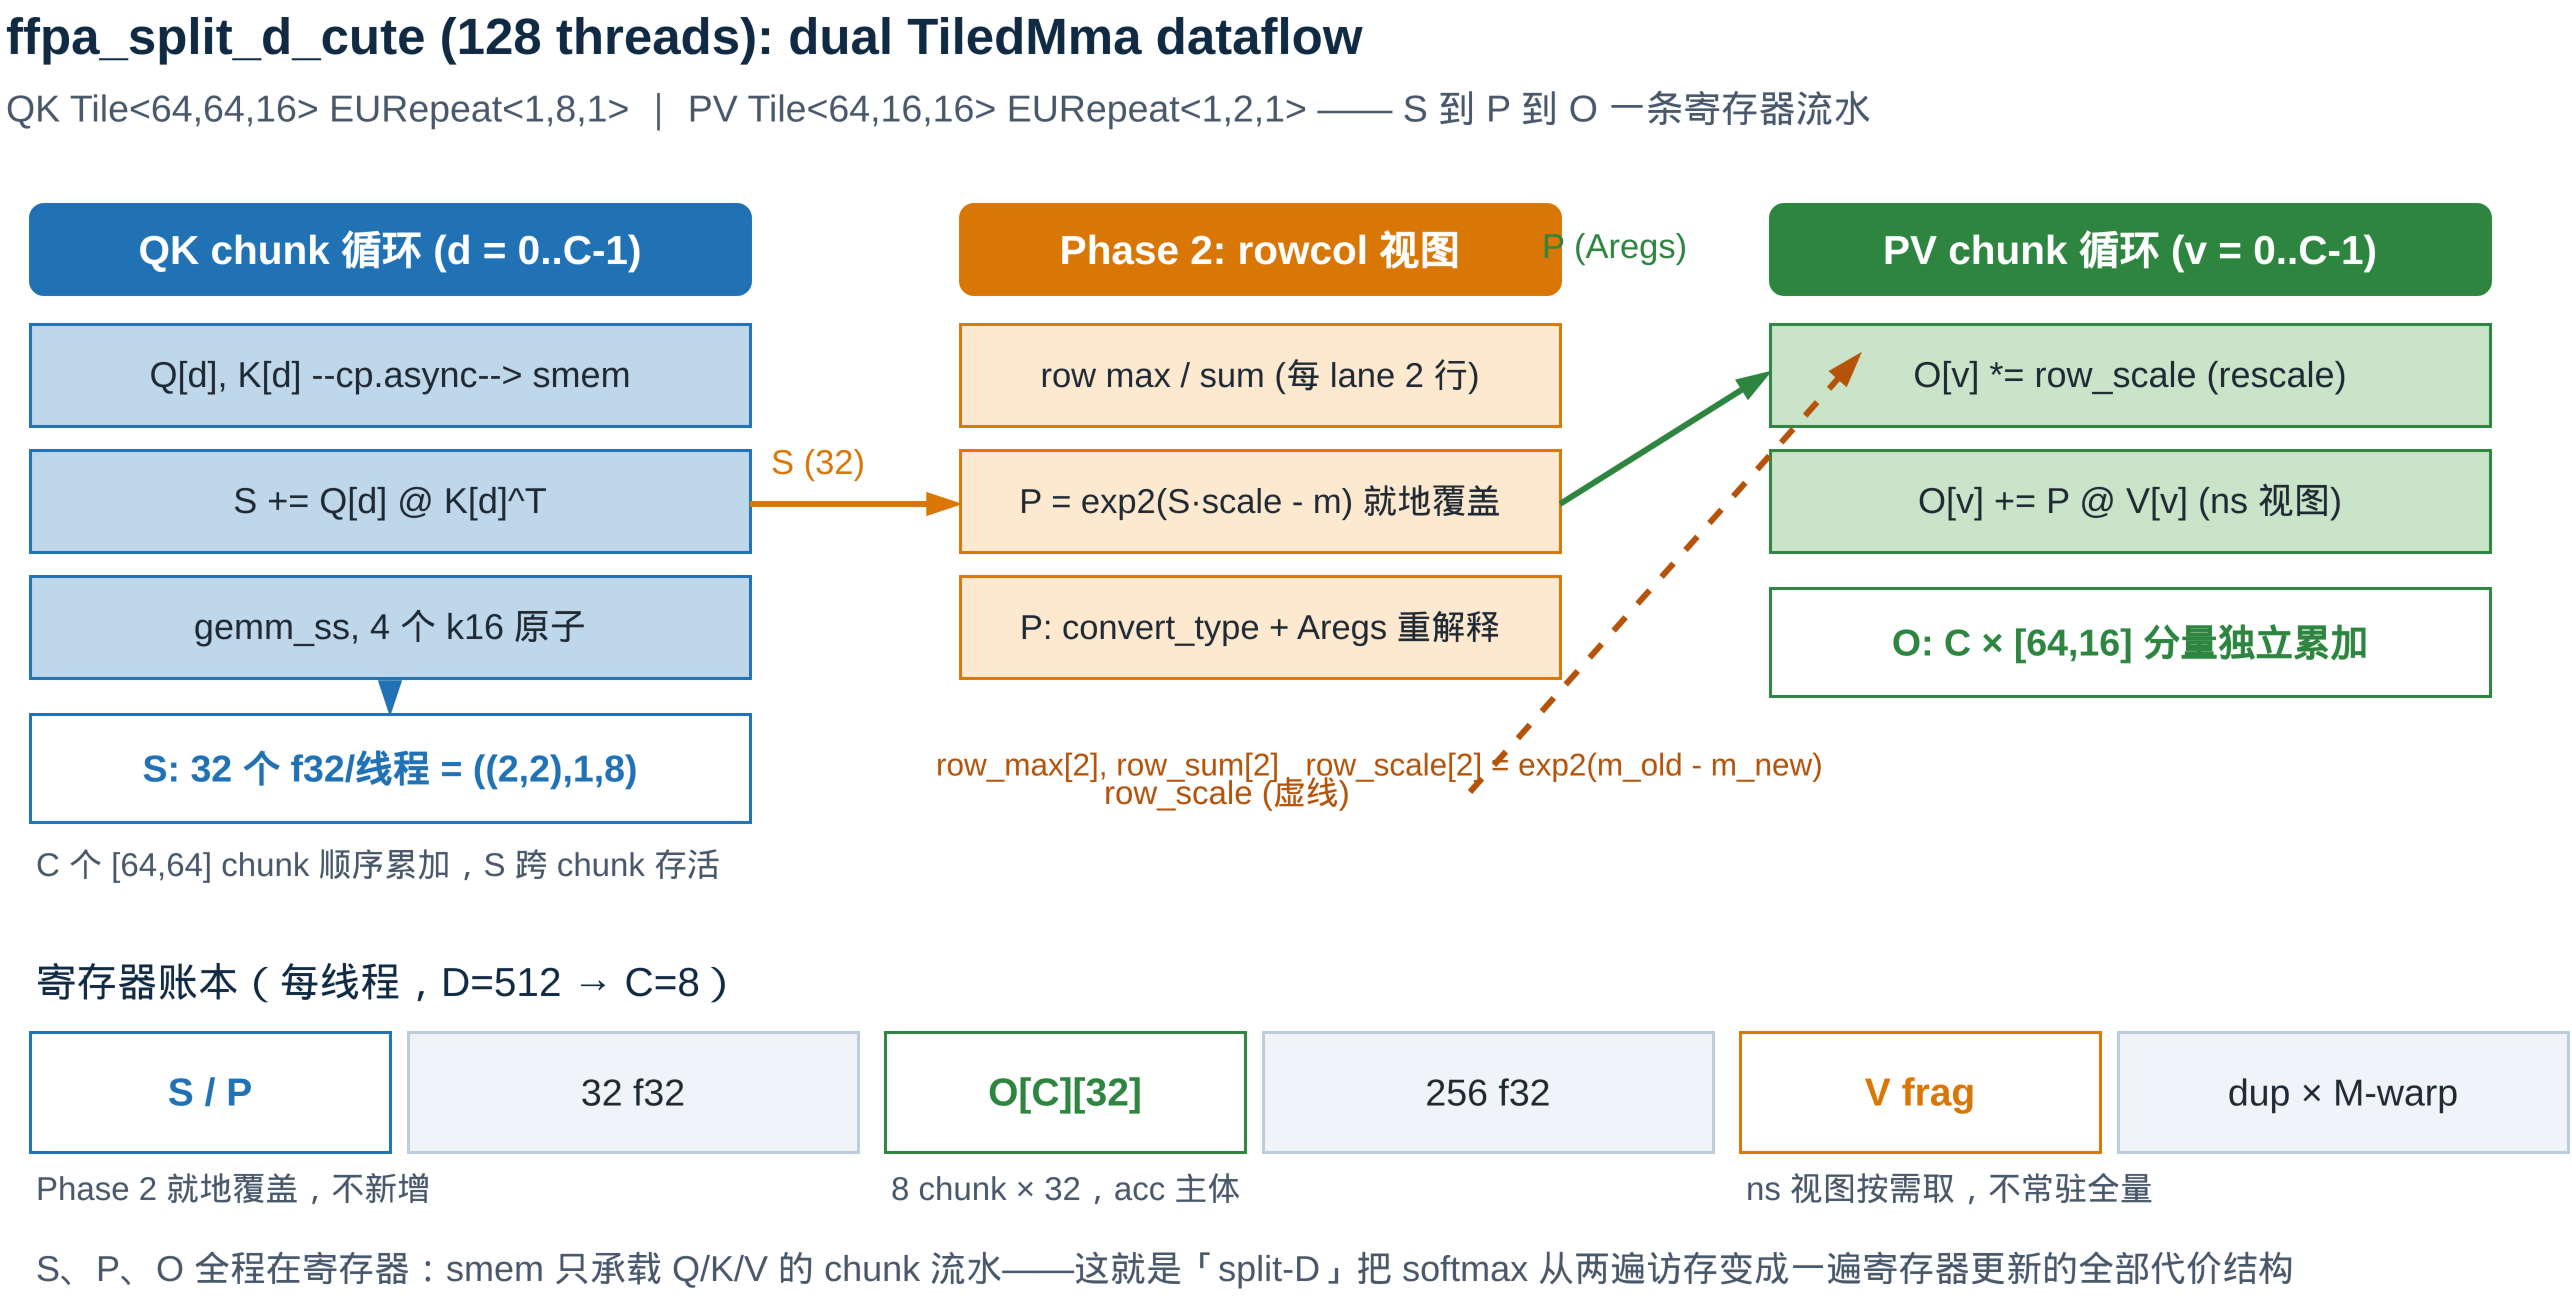
\includegraphics[width=0.92\textwidth]{figures/drawio/fig-26-1-dual-mma/fig-26-1.png}
\begin{tikzpicture}[font=\tiny, >=Stealth,
  hb/.style={align=center, inner sep=2pt, font=\bfseries\fontsize{4.6}{5.2}\selectfont},
  bx/.style={align=center, inner sep=2pt, font=\fontsize{4.2}{4.8}\selectfont},
  tx/.style={align=left, inner sep=1pt, font=\fontsize{4.2}{4.8}\selectfont, anchor=west},
]
  % 左栏：QK chunk 循环（S 累加器跨 chunk 存活）
  \node[hb, fill=tkBlue, text=white, text width=4.20cm] at (2.10,-0.12)
    {QK chunk 循环（$d = 0..C{-}1$）};
  \node[bx, draw=tkBlue, fill=tkFillBlue, text width=3.90cm] at (2.10,-0.75)
    {Q[$d$], K[$d$] $\xrightarrow{\texttt{cp.async}}$ smem};
  \node[bx, draw=tkBlue, fill=tkFillBlue, text width=3.90cm] at (2.10,-1.51)
    {S $+=$ Q[$d$] @ K[$d$]$^{\top}$};
  \node[bx, draw=tkBlue, fill=tkFillBlue, text width=3.90cm] at (2.10,-2.27)
    {gemm\_ss，4 个 k16 原子};
  \node[bx, draw=tkBlue, fill=white, text=tkBlue, text width=3.90cm,
    font=\bfseries\fontsize{4.2}{4.8}\selectfont] at (2.10,-3.03)
    {S：32 个 f32/线程 $=$ ((2,2),1,8)};
  \node[tx, text width=4.20cm] at (0,-3.55)
    {C 个 [64,64] chunk 顺序累加，S 跨 chunk 存活};
  % 中栏：Phase 2（rowcol 视图上的 softmax）
  \node[hb, fill=tkOrange, text=white, text width=3.60cm] at (6.90,-0.12)
    {Phase 2：rowcol 视图};
  \node[bx, draw=tkOrange, fill=tkFillOrange, text width=3.30cm] at (6.90,-0.75)
    {row max / sum（每 lane 2 行）};
  \node[bx, draw=tkOrange, fill=tkFillOrange, text width=3.30cm] at (6.90,-1.51)
    {scores $=$ exp2(S$\cdot$scale $-$ m) 写回 S};
  \node[bx, draw=tkOrange, fill=tkFillOrange, text width=3.30cm] at (6.90,-2.27)
    {P：convert\_type $+$ Aregs 重解释};
  \node[bx, text=tkOrange!80!black, text width=4.30cm] at (6.90,-3.05)
    {row\_max[2], row\_sum[2]\\row\_scale[2] $=$ exp2($m_{\mathrm{old}} - m_{\mathrm{new}}$)};
  % 右栏：PV chunk 循环（O 分量独立 rescale 与累加）
  \node[hb, fill=tkGreen, text=white, text width=4.20cm] at (12.30,-0.12)
    {PV chunk 循环（$v = 0..C{-}1$）};
  \node[bx, draw=tkGreen, fill=tkFillGreen, text width=3.90cm] at (12.30,-0.75)
    {O[$v$] $*=$ row\_scale（rescale）};
  \node[bx, draw=tkGreen, fill=tkFillGreen, text width=3.90cm] at (12.30,-1.51)
    {O[$v$] $+=$ P @ V[$v$]（ns 视图）};
  \node[bx, draw=tkGreen, fill=white, text=tkGreen, text width=3.90cm,
    font=\bfseries\fontsize{4.2}{4.8}\selectfont] at (12.30,-2.27)
    {O：$C \times$ [64,64] 分量独立累加（每块 4 个 N-tile）};
  % 主数据流箭头：S -> Phase 2 -> P -> PV
  \draw[->, tkOrange, semithick] (4.28,-1.45) -- (5.02,-1.45);
  \node[tx, text=tkOrange] at (4.35,-1.28) {S (32)};
  \draw[->, tkGreen, semithick] (8.78,-1.45) -- (10.18,-1.45);
  \node[tx, text=tkGreen] at (8.85,-1.28) {P (Aregs)};
  % row_scale 虚线耦合：Phase 2 尾部 -> PV 的 rescale 框
  \draw[->, dashed, tkOrange!80!black, semithick]
    (7.90,-3.42) -- (10.18,-3.42) -- (10.18,-2.42) -- (10.28,-2.42);
  \node[align=center, inner sep=1pt, font=\fontsize{4.2}{4.8}\selectfont,
    text=tkOrange!80!black] at (9.30,-3.68) {row\_scale（虚线）};
  % 底部：寄存器占用
  \node[font=\bfseries\fontsize{4.6}{5.2}\selectfont, anchor=west] at (0,-4.10)
    {寄存器占用（每线程，$D=512 \to C=8$）};
  \node[bx, draw=tkBlue, fill=white, text=tkBlue, text width=1.30cm,
    font=\bfseries\fontsize{4.2}{4.8}\selectfont] at (0.75,-4.55) {S $\to$ P};
  \node[bx, draw=gray!60, fill=gray!12, text width=2.10cm] at (2.90,-4.55) {32 f32 / 32 f16};
  \node[tx, text width=4.2cm] at (0,-4.92) {softmax 写回 S；convert\_type 生成新 P fragment};
  \node[bx, draw=tkGreen, fill=white, text=tkGreen, text width=1.30cm,
    font=\bfseries\fontsize{4.2}{4.8}\selectfont] at (5.95,-4.55) {O[$C$][32]};
  \node[bx, draw=gray!60, fill=gray!12, text width=2.10cm] at (8.10,-4.55) {256 f32 逻辑值（spill）};
  \node[tx] at (5.20,-4.92) {8$\times$32，已超 255 寄存器上限};
  \node[bx, draw=tkOrange, fill=white, text=tkOrange!80!black, text width=1.30cm,
    font=\bfseries\fontsize{4.2}{4.8}\selectfont] at (11.15,-4.55) {V frag};
  \node[bx, draw=gray!60, fill=gray!12, text width=2.10cm] at (13.30,-4.55) {每 M-warp 各一份};
  \node[tx] at (10.40,-4.92) {每线程私有，跨 warp 重复};
  \node[tx, text width=15.0cm] at (0,-5.35)
    {S/P 的更新在寄存器路径，O 的 256 个逻辑值超过 255 上限会 spill；smem 只承载 Q/K/V 的 chunk 流水——
     这就是\textbf{split-D}把 softmax 从两遍访存变成一遍寄存器更新的代价所在};
\end{tikzpicture}
\caption{双 TiledMma 的数据流：QK 沿 $D$ 累加成 $S$（32 个 f32 寄存器跨
chunk 存活），softmax 写回 $S$，再由 \texttt{convert\_type} 产生 f16 $P$，
Aregs 重解释其布局后交给 PV；$O$ 的每个 chunk 分量独立 rescale 与累加，
\texttt{row\_scale}（虚线）耦合两个循环。底部为寄存器占用：$S$ 为 32 个
f32、$P$ 为新生成的 32 个 f16 逻辑值；$O[C][32]$ 共 256 个 f32 逻辑值
（$C{=}8$，已超过 255 个寄存器的硬上限，会 spill）、V fragment 在每个
M-warp 中各有一份私有副本——smem 只承载 Q/K/V 的 chunk 流水。}
\label{fig:26-1}
\end{figure}

\section{性能分析}

本章不给新的实测数字，原因与第~\ref{ch:25}~章相同：本机没有复测 FFPA 的
完整 bench（第~\ref{ch:19}~章给出其性能数据与口径）。这里只做两件事：转录
源码注释里的既有声明（注明出处），并从本章的类型视角讨论 Split-D 抽象层的
运行时成本结构。

源码头注释（\texttt{ffpa\_\allowbreak{}attn.\allowbreak{}cuh} L16--17）的性能声明是：

\begin{quote}
  \textit{性能 (B=1,H=32,N=8192,D=512, SM120a RTX PRO 5000):
  cuDNN SDPA: 57.2 TFLOPS | FFPA TMA WS: 110.7 TFLOPS (1.94x)}
\end{quote}

读数时注意三点口径。（1）这是 TMA + WS 版（256 线程、双角色）的数字，不是
本章精读的 cp.async 版。（2）设备标称 SM120a RTX PRO 5000，而本仓库 README 的
同类标称常写 RTX 5090，同一 sm120 家族的两种卡，绝对值不可直接互比
（第~\ref{ch:19}~章的核对与 CHECKLOG 记录同此）。（3）1.94x 是相对 cuDNN SDPA
的加速比，比较对象与精度配置（f16 输入、f32 累加）需与 bench 脚本核对后才可
引用。

从类型视角看，Split-D 的抽象开销可以逐项归零：

\begin{itemize}[itemsep=2pt,topsep=2pt]
  \item \texttt{kDChunks}、\texttt{k\allowbreak{}QChunk\allowbreak{}Elements} 等全是
        \texttt{constexpr}，chunk 循环的步长、stage 偏移、池大小都在编译期
        折叠成立即数，运行时（在开启优化后）与手写版本无差别。
  \item \texttt{local\_tile}/\texttt{partition\_*} 的坐标算术全部由模板
        推导，编译产物里剩下的是少数 \texttt{mad} 与常量偏移。
  \item 实际的运行时成本在算法侧（chunk 循环的额外 barrier、V 的重复加载），
        与用不用 CuTe 无关。第~\ref{ch:19}~章对这两项开销的量化结论是
        \textbf{Stage 上限压到 2--3，同步开销主导}。
\end{itemize}

CuTe 在 Split-D 上的收益与代价都不在运行时，而在类型可断言：本章测试
（26.9 节）能在不启动 kernel 的情况下核对双 TiledMma 的每条推导。

\section{常见坑}

\textbf{坑一：推 V 的 fragment 布局必须去掉 swizzle。}
\texttt{partition\_\allowbreak{}fragment\_\allowbreak{}B} 要的是值的线程归属，而 swizzle 只改变
元素的 smem 地址。直接用带 SW128 的 \texttt{Smem\allowbreak{}Layout\allowbreak{}Vt} 去推，XOR
置换会混进逻辑坐标，fragment 布局与真值错位：正确做法是
\texttt{get\_\allowbreak{}nonswizzle\_\allowbreak{}portion} 之后再推（L137--141）。但 S2R 的
smem 地址仍由 \texttt{s2r\_thr\_v.partition\_S(sVt\_stg)} 用带 swizzle 的 storage
视图计算，两份视图职责不同。

\textbf{坑二：\texttt{convert\_\allowbreak{}type} 与 \texttt{Aregs} 的区别。}
当前源码先做类型转换、再做布局重解释（L301--303）。但
\texttt{NumericArrayConverter} 只看底层平坦数组，不按 layout 的连续段
分组；Aregs 只换索引。不能用“反序会转换错误分组”解释这段顺序，也不能
把 f32$\to$f16 的转换称为原寄存器零拷贝。

\textbf{坑三：\texttt{o\_\allowbreak{}acc\_\allowbreak{}storage} 的初始化在 chunk 循环外、只做一次。}
它在每个 kv\_tile 迭代里都是\emph{累加}目标，清零只在 kernel 开头
（L174--176）。若把它挪进 kv\_tile 循环，$O$ 会丢失历史。

\textbf{坑四：\texttt{v\_write\_pv} 的初值必须与 Phase 0 的预取数对接。}
Phase 0 写了 $\mathrm{Sv}-1$ 个 chunk，PV 循环从槽位号
$(\mathrm{Sv}-1)\bmod \mathrm{Sv}$ 继续（L308）。改 Phase 0 的预取个数
而忘了这里，会写坏正在被读的 chunk。

\textbf{坑五：chunk 循环里的 \texttt{\_\allowbreak{}\_\allowbreak{}syncthreads\allowbreak{}()} 属于槽位复用协议。}
QK 每轮末尾（L269）与 PV 每轮末尾（L350）的同步不是可有可无的：它们保证本轮
读过的 smem 槽位在下一轮被覆写之前所有线程都已读完；删掉它，表现是
高频偶发数值错误，且随 stage 数增大而加剧。

\textbf{坑六：行状态只有 2 个，但列有 16 个：shfl 掩码只到 2。}
\texttt{row\_max}/\texttt{row\_sum} 的长度是 \texttt{kORows}$=2$，
行内归约靠 \texttt{\_\allowbreak{}\_\allowbreak{}shfl\_\allowbreak{}xor\_\allowbreak{}sync} 的掩码 1 与 2（4 个 lane 一组，
L281--282 与 L291--292）。多加一层掩码 4 会把\emph{另一个 warp 段}的行
卷进来（warp 内 8 个 lane 组对应 8 个不同行块），数值立刻错。

\textbf{坑七：chunk 宽度、smem 池、TMA box 三者必须同步改。}
把 \texttt{kDChunk} 从 64 改成别的值时，SW128 原子、TMA box
（\texttt{Shape\allowbreak{}<\_\allowbreak{}64,\allowbreak{}\_\allowbreak{}64>}）、\texttt{kDChunks} 与 V 的 fragment 预计算
全部要跟着动，一个 64 改三处是这一族 kernel 改动时的固定代价。

\section{面试要点速查}

\begin{enumerate}[itemsep=3pt,topsep=3pt]
  \item \textbf{为什么 QK 的 TiledMma 要 Tile$\langle64,64,16\rangle$，
        而 PV 只要 $\langle64,16,16\rangle$？}
        QK 的 N 向 EURepeat 变成 8，一次覆盖 $S[64,64]$，省掉 N-tile
        循环（提升计算密度）；PV 的单次调用视图是 $[64,16]$，完整 O chunk
        则由 4 个 N-tile 组成 $[64,64]$，外层 V-chunk 再遍历其它 chunk。
        小 tile 控制单次调用的寄存器视图；两者的完整 C fragment 大小相同
        （$32$），因为完整输出形状与线程数相同。
  \item \textbf{Split-D 不改变 fragment 形状是什么意思？}
        $S$ 的 fragment 在 chunk 循环前后都是 $((2,2),1,8)=32$ 个 f32；
        chunk 循环表达的是同一个数组跨迭代累加。变的只是循环结构与
        归约树。
  \item \textbf{$S$ 怎么变成 $P$？为什么不需要 shuffle/smem？}
        先由 \texttt{convert\_type} 做 f32$\to$f16 数值转换并产生新 fragment；
        \texttt{convert\_\allowbreak{}layout\_\allowbreak{}acc\_\allowbreak{}Aregs} 再按 $m16n8$ 的 C 与
        $m16k16$ 的 A 映射重解释布局（C 的列向 2 值 $=$ A 的 K 向 2 值）。
        免掉的是 smem 往返，Aregs 本身仍是不搬数据的布局重解释。SM80
        $k8$ atom 的 A/C 布局相同，可拆两次 PV 继续复用；其他约定要重推。
  \item \textbf{为什么 V 的 fragment 布局要预先算、且用 nonswizzle 版本？}
        循环里只换指针不改布局——算一次省每轮推导；去掉 swizzle 是因为
        它只改地址不改值的线程归属。S2R 的 smem 地址另由
        \texttt{partition\_S} 在带 swizzle 的视图上计算。
  \item \textbf{每个线程持有多少 $O$ 逻辑累加值？}
        $C\times32$ 个 f32 \emph{逻辑累加值}：$D=512$ 时 256 个，已超过
        每线程 255 个寄存器的硬上限，实际需要 spill。第一维来自 chunk
        循环（问题尺寸），第二维来自 fragment 布局（TiledMma）。
  \item \textbf{行归约为什么要用到 \texttt{shfl\_xor} 掩码 1 和 2？}
        $m16n8$ 的 C fragment 里一行由 4 个 lane 拼成（每 lane 2 行 $\times$
        16 列），掩码 1 与 2 恰好把 4 个 lane 的两两组合并；再多就跨行块了。
  \item \textbf{smem 池的偏移为什么用指针算术而不是 layout 的 stage 维？}
        当前实现选择指针算术，不是 CuTe 的必然要求。真实的 stage mode
        应使用 stride 等于一块 chunk 元素数的非零 stride；只有 stride-0
        伪维才表示所有 stage 落到同一元素，从而使 \texttt{cosize} 与
        partition 不再对应池大小。
  \item \textbf{chunk 数与 stage 数是什么关系？}
        正交：chunk 数是问题尺寸（head\_dim/64），stage 数是流水深度
        （smem 预算）。两者的相位关系与约束见第~\ref{ch:19}~章。
\end{enumerate}

\section{最小测试与动手实验}

本章测试（\texttt{tests/\allowbreak{}ch26\_\allowbreak{}ffpa\_\allowbreak{}cute.\allowbreak{}cu}）与前几章的不同之处是
以 host 端类型断言为主：这部分不启动 kernel，只对 traits 与 fragment
做静态/运行时断言，全部来自 26.3 节的代数。下文先列这部分输出，再列 device
probe 与小规模 kernel case：

\begin{enumerate}[itemsep=2pt,topsep=2pt]
  \item \textbf{D-chunk 常量}：对 $D\in\{64,128,192,512\}$ 断言
        \texttt{kDChunks}$=D/64$ 与两个 chunk 池
        $\mathrm{cosize}=64\times64$；
  \item \textbf{双 TiledMma 推导链}：QK 的 \texttt{tile\_\allowbreak{}size\_\allowbreak{}mnk}
        $=(64,64,16)$、PV $=(64,16,16)$，线程数均为 128；
  \item \textbf{fragment 恒等式}：两个
        \texttt{partition\_\allowbreak{}fragment\_\allowbreak{}C}$((64,64))$ 的每线程元素数都是 32。
        rowcol 后的行列数 $(2,16)$；Aregs 重解释前后元素数守恒；
  \item \textbf{switch 语义}：\texttt{local\_tile} 在 $(64,64)$ tile 与
        $(row\_tile, d\_chunk)$ 坐标下的首元素地址等于
        \texttt{row\_\allowbreak{}tile*64*D + d\_\allowbreak{}chunk*64}。
\end{enumerate}

再加两个小规模 kernel 正确性 case（与第~\ref{ch:19}~章的覆盖互不重复）：

\begin{itemize}[itemsep=2pt,topsep=2pt]
  \item case E：$D=192$（3 个 chunk，且与 $\mathrm{Sk}{=}3$ 相等，用来测
        chunk 数 $=$ stage 数的边界；实际预取深度为 $\mathrm{Sk}-1=2$）、$N=128$、$H=2$、
        $\mathrm{Sk}{=}3,\mathrm{Sv}{=}2$；
  \item case F：$D=128$（2 个 chunk，$\mathrm{Sk}{=}2$）、$N=128$、$H=2$。
\end{itemize}

两者都与 CPU fp64 参考对照（容差 \texttt{TOL\_F16ACC}），运行：

\begin{lstlisting}[style=console]
cd book/tests && CUDA_VISIBLE_DEVICES=6 ./build_tests.sh --arch sm_120a --ch ch26
\end{lstlisting}

本机实测输出（sm\_120a，6 号卡）：

{\scriptsize
\begin{lstlisting}[style=console]
PASS case A chunk constants D=64 (kDChunks=1): mismatches=0 (4 checks)
PASS case A chunk constants D=128 (kDChunks=2): mismatches=0 (6 checks)
PASS case A chunk constants D=192 (kDChunks=3): mismatches=0 (8 checks)
PASS case A chunk constants D=512 (kDChunks=8): mismatches=0 (18 checks)
PASS case B dual TiledMma derivation chain (D=512): mismatches=0 (6 checks)
probe: rowcol=(2,16) aregs_elems=32
PASS case B2 device probe: rowcol (2,16) & Aregs 32 elems: mismatches=0 (3 checks)
PASS ffpa split-d cute D=192 N=128 Sk=3 Sv=2 B=1 H=2: max_abs_err=8.481e-05 (tol=5.0e-02)
PASS ffpa split-d cute D=128 N=128 Sk=2 Sv=2 B=1 H=2: max_abs_err=8.084e-05 (tol=5.0e-02)
ALL OK
\end{lstlisting}
}

\section*{延伸阅读}

\begin{itemize}[itemsep=2pt,topsep=2pt]
  \item @竹熙佳处《写给大家看的 CuTe 教程：Layout Compose \& Inverse》——
        $S\to P$ 布局变换的完整讲法（Tri Dao 的几何法与 @reed 的代数法），
        本章 26.3.3 节与第~\ref{ch:25}~章 25.3.4 节的主参考。\\
        \url{https://zhuanlan.zhihu.com/p/1962625273636845008}
  \item @reed《cute 之 高效 GEMM 实现》——TiledMMA 的组装层次、
        多级流水的写法与 Epilogue 的 smem 中转；同系列《cute 之 简单
        GEMM 实现》给出最小版本的组装范式，配合 26.3.1 的推导链与
        26.4 的相位阅读一起看。\\
        \url{https://zhuanlan.zhihu.com/p/675308830}
  \item @竹熙佳处《写给大家看的 CuTe 教程：tiled mma》——fragment 视角的
        线程-值映射，26.3.2 节两个恒等式的入门读物。\\
        \url{https://zhuanlan.zhihu.com/p/1937145378446226159}
  \item @DefTruth《FFPA(Split-D)：FA2 无限 HeadDim 扩展》——
        本主题在中文社区最系统的公开文章，Split-D 的动机与 RD 波形分析
        可与第~\ref{ch:19}~章的推导对读。\\
        \url{https://zhuanlan.zhihu.com/p/13975660308}
  \item @DefTruth《图解：从 Online-Softmax 到 FlashAttention V1/V2/V3》——
        online softmax 的图解（本书第~\ref{ch:15}~章的主参考），
        配合本章 26.3.2 的 rowcol 代数读更佳。\\
        \url{https://zhuanlan.zhihu.com/p/668888063}
  \item @66RING《使用 cutlass cute 复现 flash attention》——CuTe 版 FA 的
        工程化复现，可与第~\ref{ch:25}~章的四个实现对照。\\
        \url{https://zhuanlan.zhihu.com/p/696323042}
  \item @DeclK《CUTLASS CUTE 系列（1--5）》——布局代数与 MMA/COPY 抽象的
        系统性替代读物，作为第~\ref{ch:20}--\ref{ch:22}~章的复习材料。\\
        \url{https://zhuanlan.zhihu.com/p/1983922984805742098}
\end{itemize}

% ch26b-cute-persist-d-flash-attn.tex — CuTe 应用（四）：sm_120 持久化 FlashAttention
% ——超越 cuDNN（2026-09-22，源码 flash_attn.cuh Phase 8，L3490-4177）
% 图：全 TikZ（用户指定）；代码段引用 ../flash_attn.cuh linerange。
\chapter{CuTe 应用（四）：SM120 持久化 FlashAttention——超越 cuDNN}\label{ch:26b}

\section{本章导读}

第~\ref{ch:25}~章结束时，我们已经拿到三个 CuTe 版 FlashAttention：cp.async 统一流水、
TMA + 单 consumer warp specialization、FA3 式双 consumer。它们回答的都是布局
事实搬进类型之后 attention 长什么样，但性能口径上还缺一个对照：这些教学实现离
厂商库到底有多远？本章把三个实现里各自最强的部分拼起来，再补上两个只有在
kernel 全权可控时才做得出的优化（softmax scale$\cdot\log_2 e$ 融合、
persistent CTA），得到
\texttt{flash\_\allowbreak{}attn\_\allowbreak{}cute\_\allowbreak{}persist\_\allowbreak{}d\_\allowbreak{}sm120}
（flash\_attn.cuh L3635，\texttt{NOTES\_\allowbreak{}V2\_\allowbreak{}ENABLE\_\allowbreak{}CUTE}
宏块 Phase~8）：在 RTX PRO 5000（sm\_120，110 SM）上
$H{=}32$/$N{=}8192$/$D{=}128$ dense 场景实测 240.1 TFLOPS，为 cuDNN SDPA
（230.2 TFLOPS）的 1.04 倍。这是全书第一个在绝对性能上越过厂商库的
attention kernel。

本章的四条主线，都指向超越 cuDNN：

\begin{itemize}[itemsep=1pt,topsep=2pt]
  \item \textbf{WS 双角色}（\S\ref{sec:26b-arch}）：128 线程 producer（只发 TMA）+
        256 线程 consumer（只做 MMA），\texttt{setmaxnreg} 把 producer 的寄存器
        划给 consumer，这是 sm\_120 上把搬运与计算物理解耦的唯一手段；
  \item \textbf{Q 寄存器持久化}（\S\ref{sec:26b-persistq}）：Q tile 对整个 KV 循环
        不变，smem$\to$寄存器只搬一次，之后每次 $QK^\top$ 都是 A-operand 常驻的
        \texttt{gemm\_rs}；
  \item \textbf{softmax scale 融合}（\S\ref{sec:26b-scale-math}）：把
        $s=\text{scale}\cdot\log_2 e$ 一次性乘进 Q fragment，softmax 的 max/exp
        两个循环里的逐元素乘法全部消失；
  \item \textbf{persistent CTA}（\S\ref{sec:26b-persistent}）：dense 场景 grid
        收缩到 SM 数，每个 CTA 串行处理多个 q-tile，消除 wave 量化尾损。
\end{itemize}

\textbf{前置章节}：第~\ref{ch:15}--\ref{ch:16}~章（attention 数学与 FA2 online
softmax）、第~\ref{ch:17}~章（TMA 与 mbarrier 协议）、第~\ref{ch:21}--\ref{ch:22}~章
（TiledCopy 与 TiledMMA）、第~\ref{ch:25}~章（CuTe FA 三实现对照：本章直接复用其
五个工具函数）。\textbf{源码区间}：flash\_attn.cuh L3490--4177（Phase 8 宏块）。
\textbf{编译宏与架构}：\texttt{NOTES\_\allowbreak{}V2\_\allowbreak{}ENABLE\_\allowbreak{}CUTE}，
编译目标 \texttt{sm\_120a} 与 \texttt{sm\_120f} 均可：\texttt{setmaxnreg} 的实际
生效条件是 TMA 目的地址用 \texttt{shared::cta}，且 \texttt{\_\_launch\_\allowbreak{}bounds\_\allowbreak{}(384,~1)}
写双参数，与 arch 后缀无关（完整决策树见 \S\ref{sec:26b-setmaxnreg}）。本章 kernel
只依赖 sm\_80 级的 mma.sync 与 sm\_90 级的 TMA/mbarrier，任何 Blackwell（sm\_120）
显卡均可运行。

\section{问题与动机：为什么专用 kernel 能赢厂商库}\label{sec:26b-motivation}

手写 kernel 赢 cuDNN 在 Hopper（sm\_90）时代几乎不可信：cuDNN 在 H100 上用
WGMMA + warp specialization + TMEM 调到了接近理论峰值，普通开发者用 CuTe 从零追赶
成本极高。但 sm\_120（Blackwell 消费线/专业线）不一样：这块芯片没有
WGMMA（sm\_90 专属）、没有 tcgen05/TMEM（sm\_100 专属），cuDNN 与我们一样，
只剩同一条张量核路径：

\begin{equation*}
  \text{mma.sync.aligned.m16n8k16.row.col.f32.f16.f16.f32}
\end{equation*}

于是在 sm\_120 上，厂商库与手写的差距不再是指令代差，而全部落在协议设计
上：tile 几何、流水深度、寄存器分配、softmax 的指令数、wave 尾损。实测基线
（PRO 5000，$B{=}1$/$H{=}32$/$N{=}8192$/$D{=}128$ fp16，dense）：

\begin{center}
\begin{tabular}{lcc}
\toprule
实现 & TFLOPS & 相对 cuDNN \\
\midrule
cuDNN SDPA（\texttt{CUDNN\_ATTENTION} 后端） & 230.2 & 1.00$\times$ \\
本章 kernel & \textbf{240.1} & \textbf{1.04$\times$} \\
\bottomrule
\end{tabular}
\end{center}

领先的来源逐项拆解如下（A/B 实测，独立 kernel 上各开关单独计量）：
\texttt{exp2f} 替代 \texttt{expf}（\texttt{-{}-use\_\allowbreak{}fast\_\allowbreak{}math}，
+2\%\textasciitilde4\%）、softmax scale 融合（+3\%\textasciitilde4\%）、persistent CTA
（dense 中等序列 +2\%\textasciitilde6\%）、FA-4 条件重缩放（长序列收益，复用
第~\ref{ch:16}~章结论）。四项都是把协议里的一次浪费换成零开销，没有一项依赖复杂技巧。

还有一个工程动机：厂商库的 SDPA 对\textbf{非标准形状}（GQA 折叠、滑窗 causal、
head\_dim=96 这类非 2 的幂）经常落入慢速 fallback；专用 kernel 按自己的 tile 几何
原生支持这些形状。

\section{数学原理}\label{sec:26b-math}

\subsection{log2 域 online softmax 回顾}

第~\ref{ch:15}--\ref{ch:16}~章已经推导过 online softmax，这里只保留本章需要的形态。
对每个 KV tile，softmax 的在线更新为
\begin{align}
  m^{(t)} &= \max\!\big(m^{(t-1)},\ \max_j s_j^{(t)}\big), \label{eq:26b-max}\\
  \ell^{(t)} &= \ell^{(t-1)} e^{m^{(t-1)}-m^{(t)}} + \sum_j e^{s_j^{(t)}-m^{(t)}}, \label{eq:26b-sum}\\
  O^{(t)} &= O^{(t-1)} e^{m^{(t-1)}-m^{(t)}} + \sum_j e^{s_j^{(t)}-m^{(t)}} v_j^{(t)}, \label{eq:26b-o}
\end{align}
其中 $s_j = \text{scale}\cdot q\cdot k_j$。GPU 上把 $e^x$ 换成
$\mathrm{exp2}(x\cdot\log_2 e)$（一条 \texttt{MUFU.EX2} 即可），为此把
$\log_2 e$ 预乘进 scale：
\begin{equation}\label{eq:26b-log2domain}
  s_j^{\log_2} = \underbrace{\text{scale}\cdot\log_2 e}_{s}\cdot (q\cdot k_j),
  \qquad e^{s_j - m} = \mathrm{exp2}\!\big(s_j^{\log_2} - m^{\log_2}\big).
\end{equation}
此后所有 max/sum/rescale 都在 log2 域完成，epilogue 再乘回 $\ln 2$（若需要 lse）。

\subsection{FA-4 条件重缩放}

式~\eqref{eq:26b-sum}/\eqref{eq:26b-o} 里的 $e^{m^{(t-1)}-m^{(t)}}$ 要求每个 tile
都对 $\ell$ 和 $O$ 做一次逐元素乘法。FA-4 的观察是：随机数据下新 tile 的 max 很少
超过历史 max 太多。记 $\Delta = m^{(t-1)} - m^{(t)} \le 0$（log2 域），当
\begin{equation}\label{eq:26b-fa4}
  \Delta \ge -\tau, \qquad \tau = 8 = \log_2 256
\end{equation}
时，$2^{\Delta}$ 只会让 P 累计最多膨胀 $256\times$：fp16 的 P 最大 65504，
f32 累加器余量更大，因此可以跳过这次重缩放：$m$ 保持旧值
（stale max）、$O$/$\ell$ 原样累加。膨胀的部分在 epilogue 的 $1/\ell$ 里全部
抵消（分子分母同乘一个常数）。dense 数据下命中率高（实测 95\%+ 的 tile 满足
\eqref{eq:26b-fa4}），只有新 tile 的 max 明显更大时才付出重缩放代价。第~\ref{ch:16}~章
的手写版已经给过这个结论，本章把它原样搬进 CuTe 版
（\texttt{online\_\allowbreak{}safe\_\allowbreak{}softmax\_\allowbreak{}fa4}，
flash\_attn.cuh L3587）。

\subsection{softmax scale$\cdot\log_2 e$ 融合}\label{sec:26b-scale-math}

式~\eqref{eq:26b-log2domain} 里，$\log_2 e$ 折进 scale 只是提前一次乘法，
每个 score 元素仍然要乘 $s$ 两次：max pass 一次（\eqref{eq:26b-max}）、
exp pass 一次（\eqref{eq:26b-sum}）。对一个 $128\times 64$ 的 S tile，这是
$2\times 128\times 64 / 256\text{thread} = 64$ 次 FMUL/线程/tile，
而 QK GEMM 本身（m16n8k16 路径）每 tile 每线程只有 64 条 HMMA：softmax 的
scale 乘法指令数与 tensor core 指令数同量级，是纯浪费。

本章的优化是把 $s$ 从乘在 S 上改为乘在 Q 上：
\begin{equation}\label{eq:26b-fold}
  S_{\text{fused}} = (s\odot Q)\,K^\top = s\cdot(QK^\top) = s\cdot S_{\text{raw}},
\end{equation}
其中 $\odot$ 是逐元素乘。等价性来自两条初等性质（$s>0$）：
\begin{align}
  \max_j (s\cdot x_j) &= s\cdot \max_j x_j, \label{eq:26b-maxcommute}\\
  \mathrm{exp2}(s\cdot x - m) &= \mathrm{exp2}(S_{\text{fused},j} - m). \label{eq:26b-expcommute}
\end{align}
Q fragment 在寄存器里、对整个 KV 循环不变（persist-D），所以
\eqref{eq:26b-fold} 的代价只是 \texttt{size(tCrQ)} 次一次性 FMUL（Q s2r 后立即做），
外加 $s\odot Q$ 引入一次 fp16 重舍入。收益是 softmax 两个 pass 的逐元素乘法
归零。这条优化的前提是 persist-D：如果 Q 每个 tile 重新装载
（split-Q/FA3 布局），折叠本身也要每 tile 做一次，收益减半。

\begin{figure}[H]
\centering
\begin{tikzpicture}[
  font=\footnotesize,
  every node/.append style={align=center},
  box/.style={draw=tkBlue, fill=tkFillBlue, rounded corners=1.5pt, minimum height=0.7cm, inner sep=3pt},
  ops/.style={draw=tkPurple, fill=white, rounded corners=1.5pt, minimum height=0.7cm, inner sep=3pt},
  mul/.style={draw=tkOrange, fill=white, rounded corners=1.5pt, minimum height=0.6cm, inner sep=2pt, font=\scriptsize},
  arr/.style={-{Stealth[length=2.2mm]}, thick},
]
% before path
\begin{scope}
  \node[box] (q1) at (0,0) {$Q$};
  \node[box, right=0.5 of q1] (k1) {$K^\top$};
  \node[ops, right=0.5 of k1] (qk1) {$QK^\top$\\{\scriptsize HMMA}};
  \node[mul, right=0.35 of qk1] (m1a) {$\times s$};
  \node[mul, right=0.3 of m1a] (m1b) {$\times s$};
  \node[ops, right=0.35 of m1b] (sm1) {softmax};
  \draw[arr] (q1) -- (qk1);
  \draw[arr] (k1) -- (qk1);
  \draw[arr] (qk1) -- (m1a);
  \draw[arr] (m1a) -- node[above, font=\tiny] {max} (m1b);
  \draw[arr] (m1b) -- node[above, font=\tiny] {exp} (sm1);
  \node[font=\scriptsize\bfseries, above=0.15 of qk1] {before：每 tile 每 element 乘 2 次};
  \node[font=\tiny, tkOrange, below=0.12 of m1a] {$128{\times}64{\times}2$ FMUL / tile};
\end{scope}
% after path
\begin{scope}[shift={(0,-2.6)}]
  \node[mul] (fold) at (0,0) {$Q\times s$};
  \node[box, right=0.45 of fold] (k2) {$K^\top$};
  \node[ops, right=0.5 of k2] (qk2) {$(s\,Q)K^\top$\\{\scriptsize HMMA}};
  \node[ops, right=0.55 of qk2] (sm2) {softmax\\{\scriptsize 无乘法}};
  \draw[arr] (fold) -- (qk2);
  \draw[arr] (k2) -- (qk2);
  \draw[arr] (qk2) -- (sm2);
  \node[font=\scriptsize\bfseries, above=0.15 of qk2] {after：Q s2r 后一次性折叠};
  \node[font=\tiny, tkGreen, below=0.12 of fold] {$128{\times}D$ FMUL，全程仅一次};
\end{scope}
\end{tikzpicture}
\caption{softmax scale 融合的数据流对照。上：传统路径，S 从 QK GEMM 出来后在
softmax 的 max/exp 两个 pass 各乘一次 $s=\text{scale}\cdot\log_2 e$；
下：融合路径，$s$ 在 Q s2r 后一次性乘进 A-fragment（persist-D 使 Q 对整个
KV 循环不变），HMMA 直接输出 log2 域分数，softmax 循环体内零 FMUL。等价性由
式~\eqref{eq:26b-maxcommute}/\eqref{eq:26b-expcommute} 保证；代价是 $s\odot Q$
的一次 fp16 重舍入。}
\label{fig:26b-scale}
\end{figure}

\section{设计与实现}\label{sec:26b-design}

\subsection{总体架构：WS 双 warpgroup 与寄存器池数学}\label{sec:26b-arch}

kernel 用 384 线程、\texttt{\_\_launch\_\allowbreak{}bounds\_\allowbreak{}(384,~1)}：
前 128 线程（4 个 warp，1 个 warpgroup）是\textbf{ producer}，只做 TMA 发射与
mbarrier 维护；后 256 线程（8 个 warp，2 个 warpgroup）是\textbf{ consumer}，
只做 LDSM 装载、mma.sync、softmax。两个角色通过 K/V 的
full/empty mbarrier 对解耦（协议见 \S\ref{sec:26b-tma}）。

关键在寄存器：producer 只发 TMA（不使用 tensor core），128 个寄存器足够；
consumer 的 O 累加器（$128\times D$ f32/tile，每线程 $D/2{\times}4$ 个）+ P/S
fragment + softmax 状态却是寄存器压力的主要来源。\texttt{setmaxnreg} 让两者在
SM 寄存器池（sm\_120 为 64K/SM）里重新分配：

\begin{equation}\label{eq:26b-regpool}
  \underbrace{4\,\text{warp}\times 32\,\text{T}\times 32}_{\text{producer }400}
  + \underbrace{8\,\text{warp}\times 32\,\text{T}\times 232}_{\text{consumer }2}
  = 4096 + 59392 = 63488 < 65536 .
\end{equation}

producer 在入口执行 \texttt{warpgroup\_\allowbreak{}reg\_\allowbreak{}dealloc<32>}
（释放 96 个/线程），consumer 执行 \texttt{warpgroup\_\allowbreak{}reg\_\allowbreak{}alloc<232>}
（分配到硬件上限的可用额度）。没有这一步，consumer 会被编译器限制到每线程 168 个寄存器，
O 累加器溢出到 local memory，性能直接降低一半。

\begin{figure}[H]
\centering
\begin{tikzpicture}[
  font=\footnotesize,
  wg/.style={draw, thick, rounded corners=2pt, minimum width=4.4cm, minimum height=1.5cm, inner sep=4pt, align=center},
  arr/.style={-{Stealth[length=2.2mm]}, thick},
]
% producer
\node[wg, draw=tkBlue, fill=tkFillBlue] (prod) at (0,0)
  {\textbf{producer}：128 T（4 warp）\\
   {\scriptsize TMA 发射（Q/K/V/O）+ mbarrier}\\
   {\scriptsize \texttt{reg\_dealloc<32>}：32/线程}};
% consumer
\node[wg, draw=tkGreen, fill=tkGreen!8] (cons) at (0,-3.2)
  {\textbf{consumer}：256 T（8 warp）\\
   {\scriptsize LDSM + mma.sync + softmax + rescale}\\
   {\scriptsize \texttt{reg\_alloc<232>}：232/线程}};
% smem
\node[wg, draw=tkPurple, fill=white, minimum width=2.6cm] (smem) at (5.6,-1.6)
  {SMEM\\{\scriptsize Q persist +}\\{\scriptsize K/V stage 池}};
% arrows
\draw[arr, tkBlue] (prod.east) -- node[above, font=\tiny, sloped] {TMA 写} (smem.north west);
\draw[arr, tkGreen] (smem.south west) -- node[above, font=\tiny, sloped] {LDSM 读} (cons.east);
\draw[arr, tkOrange, dashed] (cons.north) -- node[right, font=\tiny, align=left] {k\_empty/v\_empty\\（消费完成）} (prod.south);
\draw[arr, tkBlue, dashed] (prod.south west) ++(-1.2,0) -- node[left, font=\tiny, align=right] {k\_full/v\_full\\（数据就绪）} (cons.north west);
% register pool bar
\begin{scope}[shift={(-4.2,-1.6)}]
  \draw[very thick, tkRed] (0,1.6) -- (0,-1.6);
  \fill[tkBlue!25] (0,1.55) rectangle (0.5,1.15);
  \fill[tkGreen!30] (0,1.1) rectangle (0.9,-1.55);
  \node[font=\tiny, anchor=west] at (0.55,1.35) {4096};
  \node[font=\tiny, anchor=west] at (0.95,-0.2) {59392};
  \node[font=\tiny\bfseries, anchor=south, rotate=90] at (-0.25,0) {64K/SM};
\end{scope}
\end{tikzpicture}
\caption{WS 双角色架构与 \texttt{setmaxnreg} 寄存器再分配。左：SM 寄存器池按
式~\eqref{eq:26b-regpool} 重新切分，producer 只留 32/线程，consumer 分到 232/线程；
中：producer 只发 TMA、consumer 只算；右：smem 是两者的交接面。实线箭头是数据流
（TMA 写入 $\to$ LDSM 读出），虚线箭头是 mbarrier 控制流（full = 数据就绪、
empty = 消费完成），两者构成 \S\ref{sec:26b-tma} 的握手协议。}
\label{fig:26b-arch}
\end{figure}

\subsection{smem 布局与 swizzle}\label{sec:26b-smem}

smem 按 \texttt{[Q persist | K stages | V stages]} 一维排布，总量编译期由
\texttt{kSmemElems} 决定，D=128 时 $128{\times}128{\times}2 + 2{\times}(64{\times}128{\times}2)
\times 2 = 96$\,KB（opt-in 上限 99\,KB）。每段用哪个 swizzle atom 由行字节数
决定，用的正是第~\ref{ch:23}~章的结论：

\begin{lstinputlisting}[linerange={3527-3565},firstnumber=auto,
  title={flash\_attn.cuh L3527-3565（\texttt{Flash\allowbreak{}Attn\allowbreak{}Persist\allowbreak{}D\allowbreak{}Cu\allowbreak{}Te\allowbreak{}Traits}：smem 布局与双 TiledMma）}]{../flash_attn.cuh}
\end{lstinputlisting}

三个要点。第一，swizzle atom 按 $D\times 2$\,B 对 128/64 的整除性选 SW128/SW64，
保证 LDSM 读的每个 16\,B 段不跨 swizzle 周期。第二，\texttt{Smem\allowbreak{}Layout\allowbreak{}KVt}
不是新的存储，而是 \texttt{SmemLayoutKV} 与 col-major $(D, B_c)$ layout 的
\textbf{复合}（composition）：V 物理上仍按行存，PV GEMM 的 B-operand 却以转置
视图装载（\texttt{LDSM\_T}），免去 kernel 外物化 $V^\top$。第三，Q/K/V 共用
atom 但 tile 形状不同：Q 是 $128\times D$（持久），K/V 是 $B_c\times D$
（stage 轮转），$B_c$ 按 $D$ 反推 smem 预算（D=64 时 $B_c{=}128$、
D=128 时 $B_c{=}64$，注释里给出了计算）。

\begin{figure}[H]
\centering
\begin{tikzpicture}[font=\footnotesize, scale=0.96]
% smem bar
\fill[tkFillBlue]  (0,0)    rectangle (3.4,-1.5) node[midway, align=center] {\textbf{Q persist}\\{\scriptsize $128{\times}D$}\\{\scriptsize (epilogue 复用为 sO)}};
\fill[tkBlue!12]   (3.5,0)  rectangle (5.5,-1.5) node[midway, align=center] {\textbf{K[0]}\\{\scriptsize $B_c{\times}D$}};
\fill[tkBlue!12]   (5.6,0)  rectangle (7.6,-1.5) node[midway, align=center] {\textbf{K[1]}\\{\scriptsize $B_c{\times}D$}};
\fill[tkGreen!10]  (7.7,0)  rectangle (9.7,-1.5) node[midway, align=center] {\textbf{V[0]}\\{\scriptsize $B_c{\times}D$}};
\fill[tkGreen!10]  (9.8,0)  rectangle (11.8,-1.5) node[midway, align=center] {\textbf{V[1]}\\{\scriptsize $B_c{\times}D$}};
\draw[very thick] (0,0) rectangle (11.8,-1.5);
\draw (3.45,0) -- (3.45,-1.5);
\node[font=\scriptsize, anchor=west] at (0,-1.85) {D=128, $B_c{=}64$, $S_K{=}S_V{=}2$：$32 + 16{\times}4 = 96$\,KB $\le 99$\,KB};
% stage rotation
\begin{scope}[shift={(0,-3.6)}]
  \foreach \g/\s/\col in {0/0/tkBlue, 1/1/tkBlue, 2/0/tkBlue, 3/1/tkBlue, 4/0/tkBlue}{
    \node[draw=\col, thick, fill=white, minimum width=2.28cm, font=\tiny] at (\g*2.38+1.14,0) {$g{=}\g$};
    \node[font=\tiny, anchor=north] at (\g*2.38+1.14,-0.42) {stage $s{=}\s$};
    \node[font=\tiny, tkPurple, anchor=north] at (\g*2.38+1.14,-0.78) {phase $(\g/2)\&1$};
  }
  \draw[-{Stealth}, thick, tkOrange] (0.2,0.45) -- (11.6,0.45)
    node[midway, above, font=\tiny] {全局 kv 计数 $g$（跨 q-tile 连续累计）};
\end{scope}
\end{tikzpicture}
\caption{smem 一维布局（上）与 K/V stage 轮转（下）。Q 段在 KV 循环期间只读，
循环结束后复用为 O epilogue 的 STSM 暂存（\S\ref{sec:26b-epilogue}）；K/V 各自
独立的 $S{=}2$ stage 池按全局 kv 计数 $g$ 轮转：stage $=g\bmod S$、mbarrier
相位 $=(g/S)\&1$。相位用\textbf{全局}计数而不是每 q-tile 重置，是 persistent
CTA（\S\ref{sec:26b-persistent}）与普通版协议兼容的关键。}
\label{fig:26b-smem}
\end{figure}

\subsection{TMA 装载协议：descriptor、V-first 预取与 mbarrier 相位}\label{sec:26b-tma}

Q/K/V/O 四个方向的 gmem 访问全部走 TMA。BHND packed 的张量被压平成
$(B\cdot H\cdot N, D)$ 的 2D 坐标空间，batch/head 的行偏移用
\texttt{domain\_\allowbreak{}offset} 在 kernel 内动态叠加，这样四个方向只需要
各一个 TMA descriptor（\texttt{make\_\allowbreak{}tma\_\allowbreak{}copy} 在
launcher 里构建一次，\texttt{CUTLASS\_\allowbreak{}GRID\_\allowbreak{}CONSTANT}
放进 constant memory），无论 $B/H$ 多少都不用重建。GQA 的 head 映射
（$h \mapsto h/(H/H_{kv})$）在计算 \texttt{kv\_\allowbreak{}row\_\allowbreak{}offset}
时完成。launcher 侧的构建代码只做三件事：把 BHND 压成 2D
\texttt{(total\_rows, D)} 的 gmem tensor、按 smem 布局与 box 形状各建一个
descriptor、opt-in 动态 smem：

\begin{lstinputlisting}[linerange={4104-4128},firstnumber=auto,
  title={flash\_attn.cuh L4104-4128（launcher：BHND$\to$2D 压平 + 四方向 TMA descriptor）}]{../flash_attn.cuh}
\end{lstinputlisting}

四个 tensor 的 shape 都是 \texttt{(total\_rows, D)}、stride 是
\texttt{(D, 1)}：$B/H/N$ 三个逻辑维全部折叠进行坐标，batch/head 的行偏移
(\texttt{q\_\allowbreak{}row\_\allowbreak{}offset}/\texttt{kv\_\allowbreak{}row\_\allowbreak{}offset}) 留给 kernel 内的
\texttt{domain\_\allowbreak{}offset} 动态叠加。box 形状第五个模板参 \texttt{\_1\{\}}
声明沿 minor 维（$D$）一次搬满：这正对应 Q 一次性全 $D$、K/V 整 tile
进 stage 的协议。V 与 K 共用 \texttt{SmemLayoutKV} 与同一 box 几何，差别只在
kernel 侧装载时用转置视图（\S\ref{sec:26b-smem}）。

细看 producer 的发射时序：Q 先发（一次性全 $D$），然后
K/V 各预取 $S{-}1$ 个 tile 填满流水，主循环里每个 tile 领先 $S{-}1$ 发射下一个。
注意 V-first-then-K 的顺序：V 的消费点（PV GEMM）晚于 K 的消费点
（QK GEMM）整整一段 softmax，先发 V 让 K 的 TMA 传输填进 QK 计算的空隙：

\begin{figure}[H]
\centering
\begin{tikzpicture}[
  font=\scriptsize,
  lane/.style={minimum width=1.0cm, minimum height=0.55cm, inner sep=1pt, align=center},
  arr/.style={-{Stealth[length=1.8mm]}, thick},
]
\def\lw{7.6}
% time axis
\draw[-{Stealth}] (0,1.1) -- (\lw+2.2,1.1) node[right, font=\tiny] {时间};
\foreach \t/\lab in {0.6/$t_0$, 2.6/$t_1$, 4.6/$t_2$, 6.6/$t_3$}
  \draw (\t,1.0) -- (\t,1.2) node[above, font=\tiny] {\lab};
% producer lane
\node[anchor=east, font=\scriptsize\bfseries] at (-0.2,0.35) {producer};
\node[lane, draw=tkBlue, fill=tkFillBlue, minimum width=2.0cm] at (1.6,0.35) {Q TMA};
\node[lane, draw=tkBlue, fill=tkFillBlue] at (3.1,0.35) {K0};
\node[lane, draw=tkBlue, fill=tkFillBlue] at (4.15,0.35) {K1};
\node[lane, draw=tkPurple, fill=tkPurple!8] at (5.2,0.35) {V0};
\node[lane, draw=tkPurple, fill=tkPurple!8] at (6.25,0.35) {V1};
\node[lane, draw=tkBlue, fill=tkFillBlue] at (7.3,0.35) {K2};
\node[lane, draw=tkPurple, fill=tkPurple!8] at (8.35,0.35) {V2};
\node[lane, draw=tkBlue, fill=tkFillBlue] at (9.4,0.35) {K3};
% consumer lanes
\node[anchor=east, font=\scriptsize\bfseries] at (-0.2,-0.55) {consumer};
\node[lane, draw=tkGreen, fill=tkGreen!10] at (1.6,-0.55) {Q s2r $+\,s$ 折叠};
\node[lane, draw=tkOrange, fill=orange!10, minimum width=1.4cm] at (3.0,-0.55) {QK$_0$};
\node[lane, draw=gray, fill=gray!10, minimum width=0.8cm] at (4.0,-0.55) {SM$_0$};
\node[lane, draw=tkOrange, fill=orange!10, minimum width=1.4cm] at (5.0,-0.55) {QK$_1$};
\node[lane, draw=gray, fill=gray!10, minimum width=0.8cm] at (6.0,-0.55) {SM$_1$};
\node[lane, draw=orange!20, draw=tkOrange] at (7.2,-0.55) {PV$_0$};
\node[lane, draw=orange!20, draw=tkOrange] at (8.3,-0.55) {PV$_1$};
% dependency arrows
\draw[arr, tkBlue, dashed] (3.1,0.08) -- (3.0,-0.26) node[midway, right, font=\tiny] {k\_full[0]};
\draw[arr, tkPurple, dashed] (5.2,0.08) -- (7.2,-0.26);
\draw[arr, tkOrange, dashed] (3.75,-0.55) -- (3.75,-0.9) -- (4.35,-0.9) node[midway, below, font=\tiny] {k\_empty[0]：K1 的 TMA 可以复写 stage 0};
\end{tikzpicture}
\caption{producer/consumer 流水时序（$S_K{=}S_V{=}2$ 示意）。producer 每个 KV tile
领先 $S{-}1$ 发射下一个 tile 的 TMA，且 V 先于 K 发射（V 的消费点更晚，
K 的传输得以填进 QK 计算窗口）。虚线箭头是 mbarrier 握手：\texttt{k\_full[s]}
（事务屏障，TMA 完成 + expect\_tx 校验）放行 consumer 读取；
\texttt{k\_empty[s]}（consumer 每线程 arrive）放行 producer 复写该 stage。
S tile 的 softmax（SM$_i$）与下一 tile 的 QK 在 consumer 侧串行，但与
producer 侧的 TMA 完全重叠。}
\label{fig:26b-pipeline}
\end{figure}

mbarrier 相位是这套协议最容易写错的地方。本书第~\ref{ch:17}~章用的是
每 tile 重置的相对相位；persistent CTA 下 q-tile 循环不能每轮重置
（producer 可能领先 consumer 整整一个 q-tile），所以相位改由全局
kv 计数 $g$ 决定：

\begin{equation}\label{eq:26b-phase}
  \text{stage} = g \bmod S, \qquad \text{phase} = \lfloor g/S \rfloor \&\, 1 ,
\end{equation}

$g$ 在 producer 与 consumer 两侧各自按消费序列连续累计（跨 q-tile 不清零），
wait 与 arrive 的奇偶序自然匹配。配套有一条铁律：\texttt{k\_\allowbreak{}empty}/\texttt{v\_\allowbreak{}empty}
的初始 arrive 只在第一个 q-tile 开头做一次，之后每个 stage 的
空信号完全由上一轮消费 arrive 维持。若每轮 q-tile 都补一次初始 arrive，
mbarrier 的相位会被多推一格，producer 的 wait 永远等不到正确的奇偶
（compute-sanitizer 的 synccheck 会报 \emph{Barrier error: Missing wait}）。
协议在源码里的实现分布在两侧。producer 侧（单线程发射）的主循环完整实现了
V 先 K 后、领先 $S{-}1$、按全局计数 $g$ 选 stage 与相位这套规则：

\begin{lstinputlisting}[linerange={3772-3802},firstnumber=auto,
  title={flash\_attn.cuh L3772-3802（producer 主循环：V-first-then-K 预取，$g$ 全局计数）}]{../flash_attn.cuh}
\end{lstinputlisting}

这段代码有三点需要注意。第一，\textbf{发射顺序}：循环体里 \texttt{v\_g} 的
TMA 先于 \texttt{k\_g}：V 的消费点（PV GEMM）在 K 的消费点（QK GEMM）
之后整整一段 softmax，先发 V 才能让 K 的传输填进 QK 计算窗口
（图~\ref{fig:26b-pipeline}）。第二，\textbf{stage 与相位都由 $g$ 决定}：
\texttt{g = kv\_cursor + tile + S-1} 里 \texttt{kv\_cursor} 跨 q-tile 连续累计、
循环尾统一 \texttt{+= Tc\_eff}，两行合起来就是式~\eqref{eq:26b-phase}。
第三，\textbf{事务屏障的字节数}：\texttt{arrive\_\allowbreak{}and\_\allowbreak{}expect\_\allowbreak{}tx}
声明的字节数必须精确等于该 stage 的元素数 $\times$\,\texttt{sizeof(Element)}。
TMA 完成时 mbarrier 校验的正是这个数，少一个字节都会让 consumer 的
wait 永远不满足（挂死而非出错）。consumer 侧对应的是初始 arrive 只做一次
这条铁律的落地：

\begin{lstinputlisting}[linerange={3866-3881},firstnumber=auto,
  title={flash\_attn.cuh L3866-3881（consumer：首轮一次性标记全部 stage 为 empty）}]{../flash_attn.cuh}
\end{lstinputlisting}

\texttt{if (iter == 0)} 把全部 $S_K{+}S_V$ 个 stage 的 empty 各 arrive 一次
（256 线程 \texttt{CtaBarrier} 的满额 arrive），此后每个 stage 的空位由
每次消费后的 \texttt{arrive(k\_empty[k\_stg])} 自持，与 producer 按 $g$
推进的 wait 序列恰好逐格对齐。
\subsection{Q 寄存器持久化与 \texttt{gemm\_rs}：TiledMMA/TiledCopy 组合}\label{sec:26b-persistq}

FA2 的 split-Q 布局里 Q 每个 tile 都要从 smem 重装；persist-D 的观察是：
对固定 q-tile，$Q$ 在整个 KV 循环里不变，装载一次进寄存器后，
$S = QK^\top$ 的每次计算都是 A 在寄存器、B 在 smem 的形态：第~\ref{ch:22}~章
的 \texttt{gemm\_rs} 正是为这种形态设计的。装载与折叠发生在 q-tile 循环开头：

\begin{lstinputlisting}[linerange={3883-3892},firstnumber=auto,
  title={flash\_attn.cuh L3883-3892（Q s2r 一次 + scale$\cdot\log_2 e$ 折叠进 A-fragment）}]{../flash_attn.cuh}
\end{lstinputlisting}

\texttt{partition\_\allowbreak{}fragment\_\allowbreak{}A(sQ)} 按 QK 的
TiledMMA 切出每线程的 A-fragment；\texttt{retile\_D} 把 copy 的目的视图对齐到
同一片寄存器（第~\ref{ch:21}~章的 TV-layout 分区）。折叠循环
\texttt{tCrQ(i) = (Element)(float(tCrQ(i)) * (scale * FA4\_LOG2E))} 逐元素乘
$s$ 后写回 fp16。此后 QK 的 HMMA 输出直接就是 log2 域分数
（式~\eqref{eq:26b-fold}），\S\ref{sec:26b-scale-math} 的全部收益在此兑现。

softmax 本体是 \texttt{online\_\allowbreak{}safe\_\allowbreak{}softmax\_\allowbreak{}fa4}
（L3587--3628）：与第~\ref{ch:16}~章手写版同构，差别只有两处：行/列视图来自
\texttt{convert\_\allowbreak{}layout\_\allowbreak{}acc\_\allowbreak{}rowcol}
（m16n8k16 C-fragment 的行列重解释，第~\ref{ch:22}~章），以及 scores 不再乘
scale（已经折叠）。行内 4-lane 蝶形归约（\texttt{\_\_shfl\_xor} 1 与 2）把
散在 4 个 lane 的同 row 分数归到一起：这是 m16n8k16 fragment 约定的直接
推论（每行 8 个分数由 4 个 lane 各持 2 个）：

\begin{lstinputlisting}[linerange={3587-3628},firstnumber=auto,
  title={flash\_attn.cuh L3587-3628（\texttt{online\_safe\_softmax\_fa4}：log2 域 + 条件重缩放全函数）}]{../flash_attn.cuh}
\end{lstinputlisting}

tile max 与蝶形归约在前 6 行：每行先在本地
\texttt{kSCols} 个分数里线性扫出 \texttt{tile\_max}，再 \texttt{shfl\_xor(1)} 与
\texttt{shfl\_xor(2)} 两步把 4 个 lane 的局部 max 归并成行 max：用蝶形而
非树，因为 4 lane 恰好两轮异或全覆盖。条件重缩放判定在中段：
\texttt{log2\_diff = row\_max - next\_max}，$\ge -\tau$（式~\eqref{eq:26b-fa4}）
则 \texttt{row\_scale = 1} 且 \texttt{row\_max} 保持 stale 值：本 tile 完全
跳过对 $O$/$\ell$ 的历史修正；否则 \texttt{row\_scale = exp2f(log2\_diff)}
供调用方批量重缩放。注意判定是 per-row 的，调用方用
\texttt{\_\_any\_sync} 聚合整个 warp 的是否有任一行需要重缩放，再统一
分支：warp 内分歧统一到整条 warp 粒度（L3963--3967）。exp 与求和在尾段：
\texttt{exp2f} 单条 \texttt{MUFU.EX2}，P 直接写回 scores 原地
（复用寄存器），\texttt{tile\_sum} 供 \texttt{row\_sum} 增量。

softmax 之前还有两道逐元素 mask，与式~\eqref{eq:26b-fa4} 同在 KV 主循环内：

\begin{lstinputlisting}[linerange={3940-3967},firstnumber=auto,
  title={flash\_attn.cuh L3940-3967（双 mask：KV 尾部越界列 + causal 滑窗）}]{../flash_attn.cuh}
\end{lstinputlisting}

KV 尾 mask 用 \texttt{tScS\_rc(row, col)} 的坐标视图取列号：坐标 tensor 是
identity tensor 经 TiledMMA 的 C-partition 再行列重解释得来的每线程所持
分数的 $(q, k)$ 坐标：布局问题被 CuTe 类型系统解决后，mask 只剩坐标
比较。causal mask 的 \texttt{q\_pos} 带 \texttt{kv\_offset}（$=N_{kv}-N_q$）
偏移，正是 bottom-right 对齐滑窗：$k_{pos} > q_{pos} + (N_{kv}-N_q)$ 的元素
置 $-\infty$，\texttt{exp2f} 后自然归零；整行全 mask 时 \texttt{row\_sum = 0}，
epilogue 的 \texttt{inv\_sum} 钳成 0（而非 $1/0$=NaN）：这就是
\S\ref{sec:26b-test} 里 $N_{kv}{<}N_q$ causal case 输出全 0 的机制。

PV 的 A-operand 复用第~\ref{ch:25}~章讲透的寄存器重解释技巧：
softmax 后的 P（f32 累加器 fragment）经 \texttt{convert\_\allowbreak{}type}
压成 fp16，再经 \texttt{convert\_\allowbreak{}layout\_\allowbreak{}acc\_\allowbreak{}Aregs<TiledMmaPV>}
原地重排成 PV 的 A-operand 布局：P 不落 smem，寄存器直通下一个 MMA。
V 侧则用 \S\ref{sec:26b-smem} 的转置视图 + \texttt{LDSM\_T} 装载。

\subsection{persistent CTA：wave 量化尾损与线性分配}\label{sec:26b-persistent}

非 persistent launch 的 grid $=$ q-tile 总数，硬件按 wave 调度：
110 个 SM 一波。若 tile 数是 $110k + r$（$0<r<110$），最后一个 wave 只有
$r$ 个 SM 在计算，其余空转：这就是 wave 量化尾损。$H{=}32$、
$N{=}8192$、$k_B{=}128$ 时 tile 数 $= 32\times 64 = 2048 = 18\times 110 + 68$，
最后一个 wave 尾损约 $\tfrac{110-68}{110\times 19} \approx 2\%$。

persistent CTA 的做法：grid 收缩到 $\min(\text{tiles},\ \text{SM 数})$，
每个 CTA 用 \texttt{for (cta = blockIdx.x; cta < total; cta += gridDim.x)}
线性认领多个 q-tile。尾损变成每个 CTA 多承担一小段，均匀分摊。
协议上有两个配套改动。一个是 \S\ref{sec:26b-tma} 的全局 kv 计数相位
（式~\eqref{eq:26b-phase}），另一个是 \texttt{epi\_\allowbreak{}done} 屏障：
Q smem 在 epilogue 里被复用为 O 的 STSM 暂存，producer 要装下一个 q-tile
的 Q 必须等 consumer 把 O 写完，\texttt{epi\_\allowbreak{}done}（256 线程
arrive 的 CTA 屏障）就是 Q smem 已空的确认信号。认领循环在 kernel 内
的样子（consumer 视角，producer 侧同构）：

\begin{lstinputlisting}[linerange={3853-3870},firstnumber=auto,
  title={flash\_attn.cuh L3853-3870（consumer：persistent 认领循环头与 per-tile 几何量）}]{../flash_attn.cuh}
\end{lstinputlisting}

四行坐标分解把线性 \texttt{cta} 拆回 $(b, h, q\text{-tile})$：认领顺序恰是
同一 wave 内相邻 CTA 分到相邻 tile，对 dense（tile 负载均匀）这是最优
分配。\texttt{Tc\_eff} 与 \texttt{mask\_start\_tile} 是 causal 的两个派生量：
前者把 KV 循环截到本 q-tile 可能用到的最后一格（这是 causal 减半计算量的
来源），后者标记 mask 从哪个 KV tile 开始部分可见（之前全可见，免
mask）。\texttt{q\_full} 的 wait 相位是 \texttt{iter \& 1}：q-tile 计数
奇偶，与 KV 的 $g$ 计数分属两套相位序列，互不干扰。producer 侧同位置
（L3710--3731）多两件事：\texttt{iter > 0} 时先等 \texttt{epi\_done} 的
上一轮相位（首轮免等，Q smem 天然空闲），再用 \texttt{domain\_\allowbreak{}offset}
把 head 级行偏移叠进 TMA 坐标。

\begin{figure}[H]
\centering
\begin{tikzpicture}[font=\scriptsize, scale=0.9]
% non-persistent
\begin{scope}
  \foreach \w in {0,...,4}{
    \foreach \s in {0,...,9}{
      \pgfmathtruncatemacro{\last}{\w==4 ? 3 : 9}
      \ifnum\s>\last\fill[gray!8] (\s*0.62,\w*0.5) rectangle (\s*0.62+0.62,\w*0.5+0.5);
      \else\fill[tkBlue!30] (\s*0.62,\w*0.5) rectangle (\s*0.62+0.62,\w*0.5+0.5);
      \fi
    }
  }
  \draw[very thick] (0,0) rectangle (6.2,2.5);
  \draw[tkRed, very thick, dashed] (2.48,2.0) rectangle (6.2,2.5);
  \node[font=\tiny, anchor=north] at (3.1,2.55) {wave 1（10 tile/CTA）};
  \node[font=\tiny, anchor=north] at (3.1,-0.08) {wave 3};
  \node[font=\tiny, tkRed, align=center, anchor=west] at (6.4,2.25)
    {wave 4：只有 4 个\\SM 在算\\{\bfseries 尾损 $\tfrac{6}{44}\approx 14\%$}};
\end{scope}
% persistent
\begin{scope}[shift={(9.0,0)}]
  \foreach \w in {0,...,3}{
    \foreach \s in {0,...,9}{
      \pgfmathtruncatemacro{\tail}{\w==3 ? 4 : 9}
      \ifnum\s>\tail\fill[gray!8] (\s*0.62,\w*0.5) rectangle (\s*0.62+0.62,\w*0.5+0.5);
      \else\fill[tkGreen!25] (\s*0.62,\w*0.5) rectangle (\s*0.62+0.62,\w*0.5+0.5);
      \fi
    }
  }
  \draw[very thick] (0,0) rectangle (6.2,2.0);
  \node[font=\tiny, anchor=north] at (3.1,2.05) {每 CTA 4.4 个 tile：尾损 $\tfrac{0.4}{17.6}\approx 2\%$};
\end{scope}
\node[font=\footnotesize\bfseries, anchor=south] at (3.1,2.85) {非 persistent：grid = 44 tile};
\node[font=\footnotesize\bfseries, anchor=south] at (12.1,2.85) {persistent：grid = 10 SM};
\end{tikzpicture}
\caption{wave 量化尾损示意（10 个 SM、44 个 tile 的缩小模型）。左：非
persistent launch 按整 wave 调度，最后一个 wave 只有 4 个 SM 在算，其余
空转满一个 tile 时长；右：persistent CTA 把 grid 收缩到 SM 数，每个 CTA
串行处理 $\lceil 44/10\rceil$ 或 $\lfloor 44/10\rfloor$ 个 tile，不均衡被压缩到
最后一个 tile 的零头。真实场景（110 SM，$H{=}32$/$N{=}8192$）dense 收益
+2\%\textasciitilde6\%；\textbf{causal 反向}——tile 负载前轻后重，线性分配会把
重 tile 固定在同一批 CTA 上（实测 $-9\%\sim-21\%$），此时必须回退全量 grid
让硬件调度器自然均衡。}
\label{fig:26b-persistent}
\end{figure}

dense 与 causal 的分派就在 launcher 里一行：
\begin{lstinputlisting}[linerange={4140-4151},firstnumber=auto,
  title={flash\_attn.cuh L4140-4151（launcher 的 grid 策略与 smem opt-in）}]{../flash_attn.cuh}
\end{lstinputlisting}

\subsection{Epilogue：R$\to$S(STSM)$\to$TMA store 与尾部 R$\to$G}\label{sec:26b-epilogue}

KV 循环结束后，O 累加器除以 $\ell$（FA-4 的膨胀在此全部抵消），然后按 tile
形状分两条写出路径。整 tile：寄存器 $\to$ smem（\texttt{STSM}，复用 Q 段；
此时 Q 段已闲置）$\to$ TMA store；尾部 tile（$N_q \bmod 128 \ne 0$）：
逐元素行 guard 直接 R$\to$G 写 gmem。这里有一个关键细节：producer 已经
\texttt{return} 退出，任何 \texttt{\_\_syncthreads} 都会死锁：CTA 级同步必须
换成 \texttt{Named\allowbreak{}Barrier::\allowbreak{}sync(256,~0)}（仅 consumer 参与）。
写完 O 才 \texttt{arrive} \texttt{epi\_\allowbreak{}done}，producer 由此获准复写
Q smem 装下一个 q-tile。

\begin{figure}[H]
\centering
\begin{tikzpicture}[
  font=\footnotesize,
  box/.style={draw, thick, rounded corners=1.5pt, minimum height=0.8cm, inner sep=3pt, align=center},
  arr/.style={-{Stealth[length=2.2mm]}, thick},
]
% full tile path
\begin{scope}
  \node[box, draw=tkGreen, fill=tkGreen!10] (reg) at (0,0) {O 寄存器\\{\scriptsize $\div\,\ell$、fp16}};
  \node[box, draw=tkBlue, fill=tkFillBlue] (smem) at (2.9,0) {sO（Q 段复用）\\{\scriptsize STSM}};
  \node[box, draw=tkPurple, fill=white] (gmem) at (5.9,0) {gmem O\\{\scriptsize TMA store}};
  \draw[arr] (reg) -- node[above, font=\tiny] {R$\to$S} (smem);
  \draw[arr] (smem) -- node[above, font=\tiny] {S$\to$G} (gmem);
  \node[font=\scriptsize\bfseries, above=0.1 of reg] {整 tile（$N_q \bmod 128 = 0$）};
\end{scope}
% tail path
\begin{scope}[shift={(0,-2.2)}]
  \node[box, draw=tkGreen, fill=tkGreen!10] (reg2) at (0,0) {O 寄存器\\{\scriptsize $\div\,\ell$、fp16}};
  \node[box, draw=tkOrange, fill=orange!8] (g2) at (3.6,0) {gmem O\\{\scriptsize 逐元素 row guard}};
  \draw[arr] (reg2) -- node[above, font=\tiny] {R$\to$G（行 $<N_q$ 才写）} (g2);
  \node[font=\scriptsize\bfseries, above=0.1 of reg2] {尾部 tile};
\end{scope}
% barrier note
\node[draw=tkRed, thick, rounded corners=2pt, font=\scriptsize, align=center, anchor=west] at (7.6,-1.1)
  {producer 已退出\\$\Rightarrow$ \texttt{\_\_syncthreads} 死锁\\$\Rightarrow$ \texttt{NamedBarrier(256)}\\写完 \texttt{arrive(epi\_done)}};
\end{tikzpicture}
\caption{Epilogue 双路径。整 tile 走 R$\to$S$\to$G：STSM 把 O fragment 写进
（已闲置的）Q smem 段，NamedBarrier 后由一个线程发射 TMA store——
与装载对称的反向 TMA 全链。尾部 tile 行数不足 128，STSM/TMA 的整块写
会越界，退化为带行 guard 的 R$\to$G。}
\label{fig:26b-epilogue}
\end{figure}

\section{性能分析}\label{sec:26b-perf}

主场景实测（RTX PRO 5000，110 SM，fp16）：$B{=}1$/$H{=}32$/
$N_{kv}{=}8192$/$D{=}128$。TFLOPS 按 $4BH\,N_qN_{kv}D$（causal 减半）计。

\begin{center}
\begin{tabular}{lcccc}
\toprule
场景 & 本章 kernel & cuDNN SDPA & 比值 & 备注 \\
\midrule
dense self & \textbf{240.1} & 230.2 & \textbf{1.04$\times$} & 主对照 \\
causal & 208.9 & 202.1 & 1.03$\times$ & persistent 关闭（全量 grid） \\
GQA ($H_{kv}{=}8$) & 236.1 & 218.3 & 1.08$\times$ & cuDNN 小 head 数吃亏 \\
cross ($N_q{=}1024$) & 180.7 & 165.5 & 1.09$\times$ & 短 $N_q$ 也领先 \\
$N{=}16384$ dense & 243.2 & 236.9 & 1.03$\times$ & 大 $N$ 稳定 \\
\bottomrule
\end{tabular}
\end{center}

表中每行都是成对同轮数据（kernel 与 cuDNN 同一轮测量，时钟态一致）：dense self
行为 \texttt{leetcuda\_\allowbreak{}bench\_\allowbreak{}sm120a.\allowbreak{}bin --bench}
的同轮输出（240.1/230.2，2026-09-22），其余场景为 min-of-30 复测。跨 run 的波动带：
dense 主场景 238.4/230.7、230.0/230.5、238.2/230.3、240.1/230.2（CLI bench 与 bench\_pd
两种脚本），$N{=}16384$ 为 239.2/230.9，单点绝对值跨 run 波动 $\pm2\sim3\%$
（GPU 时钟态与热态主导），但\textbf{成对比值}始终落在 $1.00\sim1.04\times$：
kernel 侧的领先是结构性的，不依赖单次测量的偶然波动。这也是本书性能复测的
通用规则：跨脚本/跨 run 的绝对值不可直接相比，结论只认同轮成对数据
（第~\ref{ch:33}~章的 bench 方法论同源）。

优化贡献的逐项拆解（同一 kernel 上各开关单独 A/B）：fast\_math
（\texttt{exp2f}）+2\%\textasciitilde4\%；scale 融合 +3\%\textasciitilde4\%（\S\ref{sec:26b-scale-math}，
指令数视角：每 tile 每线程省 64 条 FMUL，与 HMMA 数同量级）；
persistent CTA dense 中等序列 +2\%\textasciitilde6\%、causal $-9\%\sim-21\%$（分支
关闭）；FA-4 条件重缩放 dense 命中率 95\%+，与第~\ref{ch:16}~章结论一致。
各项近似可加，合计与 1.04$\times$ 的总领先吻合。

和第~\ref{ch:25}~章的三个实现纵向一比，协议设计的价值更清楚：
实现 1（cp.async 统一流水）受限于装载与计算串行；实现 2（TMA+WS 单 consumer）
解耦了搬运但 Q 每 tile 重装、softmax 带逐元素乘法、wave 尾损未作处理；
本章在实现 2 的骨架上叠加全部四项优化，同一块 GPU 上从勉强追平 SDPA
推进到稳定 +4\%。

\section{专论：SM120 上 \texttt{setmaxnreg} 的生效条件}\label{sec:26b-setmaxnreg}

本章 1.03$\sim$1.04$\times$ 的领先里，\texttt{setmaxnreg} 是 WS 双角色的物理前提
（\S\ref{sec:26b-arch}）：没有它，consumer 被编译器均分到 168 寄存器，O 累加器
溢出 local memory，性能直接降低一半。但这条指令在 SM120 工具链上是否被保留，曾被
本书两次误诊（第~\ref{ch:14}~章坑二、本节末考据框），值得用专节把全部变量
摊开。指令是否保留由\textbf{三个独立变量}决定，而 arch 后缀是其中
唯一不影响保留的一个：

\begin{center}
\footnotesize
\begin{tabular}{@{}lll@{}}
\toprule
变量 & 取值 & 后果 \\
\midrule
arch 目标 & \texttt{sm\_120a} 或 \texttt{sm\_120f} & \textbf{都完整支持并保留}（PTX ISA \\
 & & Target ISA Notes 两类均在支持列表） \\
arch 目标 & \texttt{sm\_120}（generic，无后缀） & ptxas \textbf{硬错误}——正确行为， \\
 & & 该指令只在 a/f 目标下合法 \\
TMA dst 状态空间 & \texttt{shared::cta} & 正常保留 \\
TMA dst 状态空间 & \texttt{shared::cluster} & C7506：ptxas 视作隐式 extern-call \\
 & & 边界，同 kernel 的 setmaxnreg 全部丢弃 \\
\texttt{\_\_launch\_bounds\_\_} & \texttt{(N, 1)} 双参数 & 正常保留 \\
\texttt{\_\_launch\_bounds\_\_} & \texttt{(N)} 或缺省 & C7508：PTX 不带 \texttt{.minnctapersm}， \\
 & & ``unable to determine register count'' 丢弃 \\
\bottomrule
\end{tabular}
\end{center}

\textbf{C7506（cluster 形式 TMA）}：
\texttt{cp.\allowbreak{}async.\allowbreak{}bulk.\allowbreak{}tensor} 的目的地址写成
\texttt{shared::cluster} 时，ptxas 把这条指令当作潜在的跨 CTA 副作用边界
（cluster 语义下 smem 地址可能被映射到别的 CTA），进而按 extern 调用边界
的保守规则放弃整 kernel 的寄存器再分配，只留一条 info 级 C7506，默认不打印。
第~\ref{ch:14}~章坑二的 PTX 修改（\texttt{cluster} 全局替换 \texttt{cta} 后指令恢复保留）
已给出完整取证；CUTLASS 的 \texttt{cute/arch/copy\_sm90\_tma.hpp} 在
\texttt{CUTE\_\allowbreak{}ARCH\_\allowbreak{}TMA\_\allowbreak{}SM120\_\allowbreak{}ENABLED} 门控下专门切到
\texttt{shared::cta}，上游早已知道这个差别。本 kernel 无 cluster launch、无
分布式 smem，dst 恒为 CTA 本地，两种写法语义等价，只是形式不同、保留与否不同。
\textbf{C7508（缺 launch\_bounds 第二参数）}：setmaxnreg 改变的是 per-warp
寄存器上限，ptxas 必须在 kernel 入口就知道满编时的寄存器预算才能安排池数学；
\texttt{\_\_launch\_\allowbreak{}bounds\_\allowbreak{}(N)} 只约束单 block 线程数，第二参数
（每 SM 最少驻留 block 数 = 1）才会在 PTX 生成 \texttt{.minnctapersm}。缺它，
ptxas 以 C7508 把指令全部丢弃：本章 kernel 因此声明
\texttt{\_\_launch\_\allowbreak{}bounds\_\allowbreak{}(384,~1)}。

排查方法论（每一条都有实测踩坑记录支撑）：
\begin{enumerate}[itemsep=1pt,topsep=2pt]
  \item SASS 助记符是 \texttt{USETMAXREG}（没有 n）：
        \texttt{cuobjdump -{}-dump-sass | grep setmaxnreg} 全程假阴性，本书
        两次调查都一度据此得出连最小 PTX 都被丢弃的错误结论。
  \item per-kernel 归属用
        \texttt{awk '/Function :/\{f=\$3\} /USETMAXREG/\{c[f]++\}'}；
        \texttt{-{}-function} 对 C++ mangled 模板名不匹配（报 not found，
        dump 为空，又一个假 0）。
  \item 「编译通过零警告」$\neq$「指令保留」：C7506 是 info 级默认不打印，
        验证必须加 \texttt{-Xptxas -v} 或直接数 SASS。
  \item nvcc 13.2 对每个 target 跑两个 device pass（generic 视角 +
        arch-specific 视角）：用 \texttt{\#pragma message} 探测
        \texttt{\_\_CUDA\_ARCH\_FEAT\_\allowbreak{}SM120\_\allowbreak{}ALL} 这类宏会打印出
        两遍互相矛盾的矩阵，第一遍全未定义是 generic pass 的，判断
        guard 行为必须看第二遍（arch pass）。
\end{enumerate}

2026-09-22 的终版验证矩阵（最小 probe + notes-v2 全量重编，均满足
cta TMA + \texttt{(N,1)} 双条件）：\texttt{sm\_120a} 与 \texttt{sm\_120f} 完全一致，
每 kernel 2 条（dealloc+alloc）、全二进制 6/6 条 \texttt{USETMAXREG}、零 C750x
警告；SASS 形如 \texttt{USETMAXREG.DEALLOC.CTAPOOL 0x20}。生产侧交叉印证：
ffpa-attn 的 sm\_120f 构建产物中该指令同样生效。

\begin{kaogu}[本章初版当日修正]{「必须 sm\_120f」三连误诊与推翻}
本章初版注释与导读曾断言「编译目标必须 \texttt{sm\_120f}：\texttt{sm\_120a} 下
ptxas 静默丢弃 setmaxnreg」。2026-09-22 当天三轮 probe 复核推翻该结论，
误诊链值得原样记录。先是最小 probe 的裸 asm 复现出
\emph{Instruction 'setmaxnreg' not supported on .target 'sm\_120'} 硬错误，
被读作「sm\_120a 不支持」，实际是编译命令落到了 generic \texttt{sm\_120}
（无 a/f 后缀），PTX ISA 本就不允许 generic 目标使用该指令，报错反而是
工具链在正确工作。接着 probe kernel 没写 \texttt{\_\_launch\_\allowbreak{}bounds\_\allowbreak{}(N,1)}，
ptxas 以 C7508 静默清零，又被读作 arch 问题。最后是宏探测的
\texttt{\#pragma message} 打印出两遍矛盾矩阵，第一遍（generic pass）全
未定义，进一步加深了误判。三个变量（arch 后缀 / TMA dst 状态空间 /
launch\_bounds 形态）不分离控制时，任何一个都可能被误判为 arch 问题。
这与第~\ref{ch:14}~章坑二的 2026-09-17 误诊（cluster TMA + 存活 kernel 恰好
120f 构建的两变量混同）互为镜像：一次把 TMA 形式误诊成 arch，一次把
launch\_bounds 误诊成 arch。教训同一条：单变量结论必须把另外两个变量固定后
再下。
\end{kaogu}

\section{勘误与考据}\label{sec:26b-kaogu}

本章源码为 2026-09-22 新增（Phase 8）。当日有一条正文级勘误：初版导读与
源码注释断言「编译目标必须 \texttt{sm\_120f}」，同日被三轮 probe 复核推翻
（\texttt{sm\_120a}/\texttt{sm\_120f} 都完整保留指令，实际的两个静默丢弃触发是
cluster 形式 TMA 与缺 \texttt{\_\_launch\_\allowbreak{}bounds\_\allowbreak{}(N,1)}），
已按 \S\ref{sec:26b-setmaxnreg} 的决策树全面修正，完整误诊链见该节考据框。
生产对照版（ffpa-attn 的 \texttt{persist\_\allowbreak{}d\_\allowbreak{}ws\_\allowbreak{}fwd\_\allowbreak{}cute\_\allowbreak{}sm120}）
与本章 kernel 同源，其 RFC（PC-18/PC-19）记录了 scale 融合与 persistent CTA
的生产 A/B 数据，本章表格与之交叉一致。

\section{常见坑}\label{sec:26b-pitfalls}

\begin{enumerate}[itemsep=2pt]
  \item \textbf{\texttt{setmaxnreg} 被静默丢弃}：两个独立触发，TMA 目的地址写
        \texttt{shared::cluster}（C7506，extern-call 边界），或 kernel 缺
        \texttt{\_\_launch\_\allowbreak{}bounds\_\allowbreak{}(N,~1)} 第二参数（C7508，无
        \texttt{.minnctapersm}）。两者都与 arch 后缀无关（\texttt{sm\_120a}/
        \texttt{sm\_120f} 都支持该指令），kernel 结果正确、性能降低一半，且无任何
        运行时告警。完整决策树见 \S\ref{sec:26b-setmaxnreg}。诊断口诀：SASS
        助记符是 \texttt{USETMAXREG}（没有 n），\texttt{cuobjdump -{}-dump-sass |
        grep -{}-count USETMAXREG} 为 0 即说明指令被丢弃。
  \item \textbf{persistent 初始 arrive 必须只做一次}：每 q-tile 都补
        \texttt{k\_empty} 初始 arrive 会把 mbarrier 相位多推一格，producer 的
        wait 奇偶错位（compute-sanitizer synccheck 报 \emph{Missing wait}）。
        相位改由全局计数 $g$ 决定（式~\eqref{eq:26b-phase}）后，空信号由
        消费 arrive 自持。
  \item \textbf{producer 退出后禁用 \texttt{\_\_syncthreads}}：CTA 内任何
        barrier 都必须换成仅 consumer 参与的
        \texttt{NamedBarrier}（256 线程），否则 epilogue 死锁。
  \item \textbf{gridDim 携带大数超过 65535 上限}：早期版本把
        $B\cdot H\cdot N$ 放进 \texttt{gridDim.z}，$N_q{=}4096$、$H{=}16$ 时
        恰好 $65536 > 65535$ 报 \texttt{cudaErrorInvalidValue}，于是行数改走
        kernel 参数。
  \item \textbf{依赖类型少 \texttt{typename}}：kernel 模板参数
        \texttt{Traits} 是依赖类型，直接写
        \texttt{Traits::SmemCopyAtom\{\}} 编不过；先
        \texttt{using SmemCopyAtom =} \texttt{typename Traits::SmemCopyAtom;}
        再用。第~\ref{ch:25}~章（具体类型别名）没有这个问题，本章踩过。
\end{enumerate}

\section{面试要点速查}\label{sec:26b-interview}

\begin{itemize}[itemsep=1pt]
  \item \textbf{Q：为什么你的 kernel 能赢 cuDNN？}\\
        A：sm\_120 没有 WGMMA/TMEM，双方都只能用 mma.sync；差距全在协议：
        Q 持久化省装载、scale 融合省 softmax 指令、persistent 省 wave 尾损、
        WS+TMA 流水掩盖延迟。四项合计 +4\%。
  \item \textbf{Q：scale 融合的数学依据与代价？}\\
        A：$\max(sx)=s\max(x)$（$s>0$）与 exp2 线性平移；$S_{\text{fused}}=(sQ)K^\top$。
        代价是 $s\odot Q$ 一次 fp16 重舍入（尾数 11 bit）；收益是每 tile 每
        线程 64 条 FMUL 归零。前提是 persist-D（Q 不变）。
  \item \textbf{Q：persistent CTA 为什么 causal 反而慢？}\\
        A：causal 的 tile 负载前轻后重，线性认领会把重 tail 固定在同一批
        CTA；全量 grid 让硬件调度器自然均衡。负载均匀才适合 persistent。
  \item \textbf{Q：\texttt{setmaxnreg} 的池数学？}\\
        A：$4w\times 32T\times 32 + 8w\times 32T\times 232 = 63488 < 64K$；
        producer 释放的正是 consumer 多拿的。无此指令则编译器均分 168/线程，
        O 累加器溢出。
  \item \textbf{Q：mbarrier 相位为什么用全局计数？}\\
        A：persistent 下 producer 可能跨 q-tile 领先消费，每 tile 重置相位
        无法与全局发射序对应；$g$ 连续累计 + $\lfloor g/S\rfloor\&1$ 保持
        wait/arrive 奇偶一致。
\end{itemize}

\section{最小测试与动手实验}\label{sec:26b-test}

本章测试在 \texttt{book/tests/ch26b\_\allowbreak{}fa\_\allowbreak{}persist\_\allowbreak{}d.cu}：
CPU fp64 参考对照，容差 \texttt{TOL\_F16ACC}（$5\times 10^{-2}$），十个 case 覆盖
dense / causal / GQA / Q 尾部 tile（$N_q{=}300$ 的 R$\to$G 路径）/
persistent 多迭代（$H{=}32$、$N{=}512$ 时 128 个 tile $>$ 110 SM，触发
\texttt{epi\_done} 与全局 kv 计数路径）/ KV 尾 mask（$N_{kv}{=}300$ 非
$k_{Bc}$ 倍数）/ causal 正反滑窗（$N_{kv}{>}N_q$ 与 $N_{kv}{<}N_q$，后者
前段 q 行全 mask，验证 $T_c^{eff}$ 钳零与 $L{=}0$ 行输出 0）/ $D{=}96$：

\begin{lstlisting}[style=console]
nvcc -std=c++20 -O2 -gencode arch=compute_120f,code=sm_120f \
  -DNOTES_V2_ENABLE_CUTE -I ../../third-party/cutlass/include \
  book/tests/ch26b_fa_persist_d.cu -o /tmp/ch26b_test && /tmp/ch26b_test
# PASS fa persist-D dense   D=64  B=1 H=2/2   Nq=256 Nkv=256 ...
# PASS fa persist-D dense   D=128 B=1 H=2/2   Nq=256 Nkv=256 ...
# PASS fa persist-D causal  D=128 B=1 H=2/2   Nq=512 Nkv=512 ...
# PASS fa persist-D dense   D=64  B=1 H=4/2   Nq=256 Nkv=256 ...
# PASS fa persist-D dense   D=128 B=1 H=2/2   Nq=300 Nkv=512 ...
# PASS fa persist-D dense   D=64  B=1 H=32/32 Nq=512 Nkv=512 ...
# PASS fa persist-D dense   D=128 B=1 H=2/2   Nq=256 Nkv=300 ...
# PASS fa persist-D causal  D=64  B=1 H=2/2   Nq=256 Nkv=512 ...
# PASS fa persist-D causal  D=128 B=1 H=2/2   Nq=512 Nkv=256 ...
# PASS fa persist-D dense   D=96  B=1 H=2/2   Nq=256 Nkv=256 ...
# ALL OK
\end{lstlisting}

集成入口在 bench/flash\_attn.cu（\texttt{test\_\allowbreak{}flash\_\allowbreak{}attn\_\allowbreak{}cute\_\allowbreak{}persist\_\allowbreak{}d\_\allowbreak{}sm120}，
含 $N_q{=}2048$/$H{=}8$ 的多 q-tile 大 case）。参考实现用 \textbf{cuDNN SDPA}
（\texttt{NOTES\_\allowbreak{}V2\_\allowbreak{}ENABLE\_CUDNN} 构建下经 cudnn-frontend 组图：
GQA 按 $h\mapsto h/(H/H_{kv})$ 折叠、causal 用 bottom-right 对齐，恰是本
kernel 的滑窗 mask 语义）；cuDNN 不覆盖的组合（$N_q>N_{kv}$ 的 causal，
bottom-right 对角线出界）自动回退 CPU fp64。输出行的 \texttt{ref=} 字段标记
当轮参考来源，fp64 CPU 参考从每 case 数十秒缩到 cuDNN 的亚秒级：

\begin{lstlisting}[style=console]
$ ./leetcuda_bench_sm120a.bin --pd-cute
| FA persist-D WS persistent CTA scale-fused (D=64, Nq=2048, Nkv=2048, \
Hq=8, Hkv=8, ref=cudnn) | 3.052e-05 |
| FA persist-D WS persistent CTA scale-fused (D=128, Nq=1024, Nkv=1024, \
Hq=2, Hkv=2, causal, ref=cudnn) | 4.883e-04 |
| FA persist-D WS persistent CTA scale-fused (D=64, Nq=1024, Nkv=1024, \
Hq=4, Hkv=2, ref=cudnn) | 6.104e-05 |
| FA persist-D WS persistent CTA scale-fused (D=128, Nq=512, Nkv=256, \
Hq=2, Hkv=2, causal, ref=cpu) | 3.363e-04 |
=== persist-D cute tests done ===
\end{lstlisting}

性能复测有两条口径。\texttt{-{}-bench -{}-bhnd 1,32,8192,128}：本 kernel 作为
FA 家族最快实现排在 bench 末位默认运行，与 cuDNN SDPA（f32 compute）同轮
成对对照：\texttt{| FA2 CuTe TMA MMA Persistent-CTA WS (D=128) | 1.526e-05
| 238.4/230.7 (1.03x) |}（\S\ref{sec:26b-perf} 复测带数据）；
独立脚本 \texttt{bench\_pd.cu}（\texttt{book/.tmp/ch26b/}，dense/causal/GQA/$N$
扫描）与初版表格数据，全部归档 \texttt{.tmp/book-bench/ch26b/}。动手实验建议：
(1) 把 \texttt{FA4\_\allowbreak{}RESCALE\_\allowbreak{}THRESHOLD} 调成 0
观察 FA-4 跳过率归零后的性能退化；(2) 强制 dense 也用全量 grid，
验证 \S\ref{sec:26b-persistent} 的 wave 尾损数字；(3) 去掉 Q s2r 后的
折叠循环，把 scale 乘法放回 softmax，复测 scale 融合的贡献；(4) 用
\texttt{cuobjdump -{}-dump-sass | grep -{}-count USETMAXREG} 验证
\S\ref{sec:26b-setmaxnreg} 的两个静默丢弃触发：临时去掉
\texttt{\_\_launch\_\allowbreak{}bounds\_\allowbreak{}(384,~1)} 的第二参数重编，
数指令归零并观察 C7508 警告（需 \texttt{-Xptxas -v}）。

\section*{延伸阅读}

\begin{itemize}[itemsep=1pt]
  \item FlashAttention-3 论文 \S3.1.4（conditional rescaling 的原始定义与
        $\tau$ 的选取依据）；
  \item CUTLASS 77\_blackwell\_fmha（FA-4 式 softmax 在 Blackwell 上的
        warp-uniform rescale 与 TMEM 形态，可对照本章 per-row 形态）；
  \item @DefTruth《图解：从 Online-Softmax 到 FlashAttention V1/V2/V3》
        （online softmax 推导基线，本书第~\ref{ch:15}--\ref{ch:16}~章同源）；
  \item ffpa-attn RFC PC-18/PC-19（scale 融合与 persistent CTA 的生产版
        A/B 数据与量化家族适用性盘点）。
\end{itemize}

% ch26c-cute-split-d-sm120.tex — CuTe 应用（五）：SM120 大 head_dim Split-D
% non-WS 全员 MMA 流水（2026-09-23，源码 ffpa_attn.cuh L642-1307）
% 图：全 TikZ（沿用 ch26b 先例）；代码段引用 ../ffpa_attn.cuh linerange。
\chapter{CuTe 应用（五）：SM120 大 head\_dim Split-D——non-WS 全员 MMA 流水}\label{ch:26c}

\section{本章导读}

第~\ref{ch:26}~章结束的时候，Split-D 的 CuTe 版实测 140.2 TFLOPS：
64$\times$64 tile、TMA + warp specialization、单 consumer warpgroup。它把
大 $D$ 分块的类型代数讲清楚了，但执行协议还是教学级的。本章
把 ffpa-attn 的 non-WS CuTe TMA kernel（\texttt{csrc/cuffpa/cute/sm\_120/split\_d.cuh}）
以最小教学集移植进本书源码（ffpa\_attn.cuh L642--1307，\texttt{NOTES\_\allowbreak{}V2\_\allowbreak{}ENABLE\_\allowbreak{}CUTE}
与 \texttt{NOTES\_\allowbreak{}V2\_\allowbreak{}ENABLE\_\allowbreak{}TMA\_\allowbreak{}MMA\_\allowbreak{}WS}
双宏块）。本实现与 ffpa-attn 的 cute sm\_120 split\_d \textbf{同源}，
在 RTX PRO 5000 上把 $B{=}1$/$H{=}32$/$N{=}8192$/$D{=}320$
dense 场景做到 \textbf{204.1 TFLOPS}——cuDNN SDPA（69.7）的 2.93 倍、
上一章 WS 教学版（140.2）的 1.46 倍。这一性能是全书大 head\_dim 路线的最高值。

本章的四条主线，每一条都是对 WS 教学版某个具体弱点的回应：

\begin{itemize}[itemsep=1pt,topsep=2pt]
  \item \textbf{tile 128$\times$128 与 M8N1 TiledMma}（\S\ref{sec:26c-tile}）：
        同一份 K/V smem 数据服务的 Q 行翻倍，算术强度上一档；
        8 个 warp 全部沿 M 堆叠、N 不切分，每 warp 持整行，
        softmax 行归约退化为 warp 内 4-lane 蝶形，零跨 warp 通信；
  \item \textbf{non-WS 执行模型}（\S\ref{sec:26c-nonws}）：256 线程全员
        MMA，\texttt{tid=0} 在消费循环里内联发射 TMA——WS 版有 128 个
        producer 不产 FLOPs，参与 MMA 的 warp 数只有一半。warp 数不直接
        等于 Tensor Core 吞吐，但少了整组 producer 是明确的结构性成本；
        non-WS (2,2) 相对 WS (2,2) 的 140.2$\to$188.3 还同时叠加了
        tile 从 64 升到 128 等因素，不能把全部差值归因于 warp 数。
        QK 与 PV 两套互不相交的 barrier 集支撑起独立流水深度，
        并让下一 kv\_tile 的 QK 预取与本 tile 的 softmax+PV 重叠；
  \item \textbf{STSM + TMA store 批量 epilogue}（\S\ref{sec:26c-epilogue}）：
        O 累加器经 \texttt{stmatrix} 暂存（复用已释放的 QKV smem）再按
        bulk group 批量 TMA 写回，替代 WS 版的逐元素寄存器直写 gmem；
  \item \textbf{FA-4 条件重缩放与流水深度解耦}（\S\ref{sec:26c-rescale}、
        \S\ref{sec:26c-perf}）：max 增长不足 $2^8$ 时跳过整个
        $O$ 重缩放循环（warp vote 保证无分支发散）；$S_K$ 与 $S_V$
        作为独立模板参数分开调，实测 D$\le$320 最优组合是 $(3,2)$：
        加深 QK 流水 +8.4\%，加深 V 流水反而降低性能。
\end{itemize}

\textbf{前置章节}：第~\ref{ch:15}--\ref{ch:16}~章（attention 数学与 online
softmax）、第~\ref{ch:17}~章（TMA 与 mbarrier 协议）、第~\ref{ch:19}~章
（Split-D 的 chunk 分解数学与寄存器占用——本章不再重推）、第~\ref{ch:21}--\ref{ch:23}~章
（TiledCopy/TiledMMA/swizzle）、第~\ref{ch:25}--\ref{ch:26}~章（CuTe FA
工具函数与 WS 版类型代数）、第~\ref{ch:26b}~章（FA-4 条件重缩放的数学，
式~(26b.5)）。\textbf{源码区间}：ffpa\_attn.cuh L642--1307。\textbf{编译宏}：
\texttt{NOTES\_\allowbreak{}V2\_\allowbreak{}ENABLE\_\allowbreak{}CUTE} +
\texttt{NOTES\_\allowbreak{}V2\_\allowbreak{}ENABLE\_\allowbreak{}TMA\_\allowbreak{}MMA\_\allowbreak{}WS}，
目标 \texttt{sm\_120a}。kernel 只依赖 sm\_80 级 mma.sync 与 sm\_90 级
TMA/mbarrier/STSM，任何 Blackwell 显卡可运行。\textbf{教学裁剪}：无
bias/dropout/GQA/NHD/causal；保留 Nkv 边界 mask 与 LSE 输出；
要求 $N_q \bmod 128 = 0$（epilogue 恒走整 tile STSM+TMA 路径）。

\section{问题与动机：WS 教学版慢在哪里}\label{sec:26c-motivation}

先把数据摆开。同一块 RTX PRO 5000（110 SM）、同一 bench 口径
（$B{=}1$/$H{=}32$/$D{=}320$ fp16 dense，成对同轮测量）：

\begin{center}
\begin{tabular}{lccc}
\toprule
实现 & TFLOPS & 相对 cuDNN & 相对 WS(2,2) \\
\midrule
cuDNN SDPA & 69.7 & 1.00$\times$ & --- \\
WS 教学版 (1,1)（第~\ref{ch:26}~章） & 86.7 & 1.24$\times$ & 0.62$\times$ \\
WS 教学版 (2,2) & 140.2 & 2.01$\times$ & 1.00$\times$ \\
本章 non-WS (2,2) & 188.3 & 2.70$\times$ & 1.34$\times$ \\
本章 non-WS (3,3) & 188.5 & 2.70$\times$ & 1.34$\times$ \\
\textbf{本章 non-WS (3,2)} & \textbf{204.1} & \textbf{2.93$\times$} & \textbf{1.46$\times$} \\
\bottomrule
\end{tabular}
\end{center}

（本章实现与 ffpa-attn 的 cute sm\_120 split\_d 同源，stages 同样
经模板参数独立可调；上表只对照本章自有的 WS 教学版与 cuDNN。）

从 140 到 204 的 45\% 差距，逐项拆开是四个结构性问题。

\textbf{第一，WS 的代价：producer 不产 FLOPs。}WS 教学版 256 线程里
128 个是 producer（只发 TMA），实际做 MMA 的只有单 consumer warpgroup
的 128 线程。SM 上 MMA warp 数降低一半。

第~\ref{ch:26b}~章的 D=128 场景里，WS 换来的是 Q 持久化与
\texttt{setmaxnreg} 的寄存器再分配，收益大于成本。但 Split-D 的 O 累加器
（$32 \times C$ 个 f32/线程，第~\ref{ch:19}~章寄存器占用）本来就把寄存器
预算占用到 255 上限附近，
\texttt{setmaxnreg} 腾不出多少寄存器，WS 的收益消失、成本全留。
这是大 $D$ 路线选 non-WS 的根本理由。

\textbf{第二，tile 64$\times$64 的算术强度太低。}K/V 的一个
$64\times D$ chunk 从 gmem 搬进 smem，只服务 64 行 Q。tile 升到
$128\times128$ 后同一份 K/V 服务 128 行 Q，搬运量减半而计算量不变。
更关键的是 smem 预算：64$\times$64 tile 时 chunk 宽 64，128$\times$128
tile 时若 chunk 仍取 64，$Q{+}K$ 每 stage 要
$128{\times}64{\times}2 \times 2 = 32$\,KB；把 Q/K chunk 降到 32（V/O 保持
64），每 stage 只要 16\,KB，同预算就能装下更宽的 tile 与更深的流水。
chunk 宽 32 的 swizzle 相应从 SW128 退到 SW64。SW64 的 atom 是
$8\times32$ half，即 8 行 $\times$ 64\,B $=$ 512\,B；单行 64\,B 只是模式
跨度，完整的 XOR 图样仍跨 8 行（\S\ref{sec:26c-tile}）。

\textbf{第三，写回通道逐元素化。}WS 教学版的 epilogue 是寄存器逐元素
直写 gmem（每线程 32 个 $C$ 分量循环写）。non-WS 版走完整反向链：
f16 转换 $\to$ \texttt{stmatrix}（STSM）暂存 smem $\to$ TMA store 批量
写回，与装载的 TMA 全链对称。

\textbf{第四，每 tile 的 rescale 大多不必要。}FA-2 式无条件重缩放在
$D{=}320$（每 kv\_tile 10 个 QK chunk、5 个 PV chunk）下，每个 tile
都要对 160 个 f32 寄存器的 O 累加器乘一次 \texttt{row\_scale}。FA-4 的
条件重缩放（第~\ref{ch:26b}~章式~(26b.5)，$\tau = 8$）让 95\%+ 的 tile
整个跳过这个循环。

还有一项无额外代价的结构收益：跨 kv\_tile 预取。WS 版的
producer/consumer 分工里，下一 tile 的装载要等本 tile 消费腾出 stage；
non-WS 版把 QK 与 V 拆成两套互不相交的 barrier 集，下一 tile 的 QK
初始 chunk 可以在本 tile 的 softmax+PV 窗口里提前发出（\S\ref{sec:26c-prefetch}）。

\section{协议设计}

\subsection{tile 几何与 smem 预算：chunk 解耦}\label{sec:26c-tile}

协议全部参数集中在 traits 里，取值如下：

\begin{lstinputlisting}[linerange={701-722},firstnumber=auto,
  title={ffpa\_attn.cuh L701-722（traits：协议参数与 smem 公式）}]{../ffpa_attn.cuh}
\end{lstinputlisting}

四组参数的分工如下。tile 几何：$k_{Br}{=}k_{Bc}{=}128$，
$k_{NumThreads} = 128/16 \times 32 = 256$。chunk 解耦：
$k_{QKDChunk}{=}32$、$k_{VDChunk}{=}64$，即 Q/K 与 V/O 的 D 向切块宽度
不同，$k_{DChunksQK} = D/32$ 个 QK chunk 对 $k_{DChunksV} = D/64$ 个
PV chunk（D=320 时 10 对 5）。流水深度解耦：
$k_{StagesQK}$ 与 $k_{StagesPV}$ 是两个独立模板参数，\S\ref{sec:26c-perf}
的实验会证明最优值是 $(3,2)$ 而不是对称的 $(3,3)$。smem 公式：
\begin{equation}\label{eq:26c-smem}
  \text{smem} = \underbrace{S_K \cdot (128{\times}32 + 128{\times}32)}_{\text{Q+K，每 stage }16\text{KB}}
  \;+\; \underbrace{S_V \cdot 128{\times}64}_{\text{V，每 stage }16\text{KB}}
  \;=\; 16\,(S_K + S_V)\ \text{KB} ,
\end{equation}
$(2,2){=}64$\,KB、$(3,2)/(2,3){=}80$\,KB、$(3,3){=}96$\,KB（fp16）。
Q 每 kv\_tile 重装（它不属于持久化协议），所以 Q 也占用 $S_K$ 份 stage。
注意 smem 与 $D$ 无关：chunk 宽度固定，$D$ 只决定 chunk 个数。

chunk 宽度还决定 swizzle atom 的选择，规则与第~\ref{ch:23}~章一致
（行字节数 $\times$ 2B 对 128/64 的整除性），但这里按 chunk 而不是按
$D$ 选：

\begin{lstinputlisting}[linerange={730-756},firstnumber=auto,
  title={ffpa\_attn.cuh L730-756（chunk 尺寸决定 swizzle；M8N1 双 TiledMma；装载/写回 atom）}]{../ffpa_attn.cuh}
\end{lstinputlisting}

Q/K chunk 行宽 32$\times$2$=$64\,B，SW64 的模式跨度与单行匹配；但
\texttt{Layout\_K\_SW64\_Atom} 是 $8\times32$ half（8 行、512\,B），
完整 XOR 图样跨 8 行，不能把单行 64\,B 当成一个完整周期。用 SW128 会
把行 padding 到 128\,B；V/O chunk 行宽 128\,B 落回 SW128。\texttt{SmemLayoutVt} 是 V 的转置视图（composition，不
物化），PV 的 B-operand 以 $D_c \times B_c$ 列主视图交给
\texttt{LDSM\_T}。\texttt{SmemLayoutO} 与 V 同 atom，epilogue 复用已
释放的 QKV smem 时布局保持一致（\S\ref{sec:26c-epilogue}）。

\subsection{M8N1 TiledMma：warp 持整行，softmax 归约零跨 warp}\label{sec:26c-mma}

QK 与 PV 共用 m16n8k16 atom（sm\_120 唯一张量核路径，第~\ref{ch:26b}~章
已论证），差别在 TiledMma 的 warp 排布。两处 \texttt{Layout<Shape<8,1,1>>}
把 8 个 warp \textbf{全部沿 M 堆叠、N 不切分}（M8N1）：每个 warp 独占
$S$ tile 的 16 行，整行不切。这带来一个 softmax 侧的收益：
m16n8k16 的 C-fragment 约定下，一行 128 个分数散在同 warp 的 4 个 lane
（每 lane 2$\times$8 列块中的 2 份），行 max / 行 sum 的归约只需要
warp 内 \texttt{\_\_shfl\_xor} 两轮（1 与 2 的蝶形，\S\ref{sec:26c-rescale}），
没有任何跨 warp 的 smem 归约。

本章与第~\ref{ch:26}~章的行归约同构：那边是 4 warp $\times$ 16 行 $= 64$
行 tile，这边是 8 warp $\times$ 16 行 $= 128$ 行 tile，两者的跨 warp
通信都为零。代价是 PV 的 N 维只有 $k_{VDChunk}{=}64$：
单 warp 的 PV MMA 每次算 $16\times64$，由
\texttt{gemm\_rs}（第~\ref{ch:25}~章）内部按 atom 循环展开，不影响
协议。

装载/写回 atom：Q/K 用 \texttt{U32x4\_LDSM\_N}（128 bit 对齐直读），
V 用 \texttt{U16x8\_LDSM\_T}（转置装载），O 写回用
\texttt{SM90\_U32x4\_STSM\_N}（\texttt{stmatrix}，\S\ref{sec:26c-epilogue}）。

\subsection{non-WS 执行模型：全员 MMA 与内联 TMA}\label{sec:26c-nonws}

\begin{figure}[H]
\centering
\begin{tikzpicture}[
  font=\footnotesize,
  wg/.style={draw, thick, rounded corners=2pt, minimum width=5.2cm, minimum height=1.35cm, inner sep=4pt, align=center},
  arr/.style={-{Stealth[length=2.2mm]}, thick},
]
% WS side
\begin{scope}
  \node[wg, draw=tkBlue, fill=tkFillBlue] (prod) at (0,0)
    {\textbf{producer}：128 T（4 warp）\\
     {\scriptsize 专职 TMA 发射 + mbarrier，产 0 FLOPs}};
  \node[wg, draw=tkGreen, fill=tkGreen!8] (cons) at (0,-2.9)
    {\textbf{consumer}：128 T（4 warp）\\
     {\scriptsize LDSM + mma.sync + softmax}};
  \node[wg, draw=tkPurple, fill=white, minimum width=2.2cm, minimum height=2.6cm] (smem) at (4.4,-1.45) {SMEM\\{\scriptsize 64$\times$64}\\{\scriptsize tile}};
  \draw[arr, tkBlue] (prod.east) -- node[above, font=\tiny, sloped] {TMA} (smem.north west);
  \draw[arr, tkGreen] (smem.south west) -- node[above, font=\tiny, sloped] {LDSM} (cons.east);
  \node[font=\scriptsize, anchor=north] at (2.0,-4.4) {MMA warp 数 = 4/SM slot};
\end{scope}
% non-WS side
\begin{scope}[shift={(9.6,0)}]
  \node[wg, draw=tkGreen, fill=tkGreen!8] (all) at (0,-1.45)
    {\textbf{全员 consumer}：256 T（8 warp）\\
     {\scriptsize LDSM + mma.sync + softmax + rescale}\\
     {\scriptsize \texttt{tid=0} 内联发射 TMA（非专职）}};
  \node[wg, draw=tkPurple, fill=white, minimum width=2.2cm, minimum height=2.6cm] (smem2) at (4.4,-1.45) {SMEM\\{\scriptsize 128$\times$128}\\{\scriptsize tile}};
  \draw[arr, tkOrange] (all.east) to[bend left=18] node[above, font=\tiny, sloped] {tid=0 TMA} (smem2.north west);
  \draw[arr, tkGreen] (smem2.south west) -- node[above, font=\tiny, sloped] {全员 LDSM} (all.east);
  \node[font=\scriptsize, anchor=north] at (2.0,-4.4) {MMA warp 数 = 8/SM slot（$\times$2）};
\end{scope}
% vs marker（两图空隙中点：左 smem 右缘 5.5，右 consumer 左缘 7.0）
\node[font=\large\bfseries, tkRed] at (6.25,-1.45) {vs};
\end{tikzpicture}
\caption{WS 与 non-WS 执行模型对照。左（第~\ref{ch:26}~章 WS 教学版）：
128 线程专职 producer 与 128 线程 consumer 分工，smem 为交接面——搬运与
计算解耦的代价是 SM 上做 MMA 的 warp 只剩一半。右（本章）：256 线程全员
consumer，\texttt{tid=0} 在消费循环内联发射 TMA（发射指令本身不占独立
warp 的时间片，只占少量指令槽）；tile 同步升到 128$\times$128，MMA warp
数从 4 增至 8，算术强度随之提高。大 $D$ 下 O 累加器占满寄存器预算，
\texttt{setmaxnreg} 腾不出寄存器，WS 的收益消失——non-WS 成为唯一选择。}
\label{fig:26c-arch}
\end{figure}

non-WS 不等于关掉 warp specialization：它要求发射 TMA 的线程同时是
消费线程，由此带来两个协议约束。第一个约束是发射点必须挂在消费依赖
之后：\texttt{tid=0} 要复写某个 stage，必须先等全 CTA 的
256 个线程都消费完（\texttt{qk\_empty} 的 init count 是
$k_{NumThreads}$），而 \texttt{tid=0} 自己也是消费者之一。预取代码若
挪到 \texttt{gemm\_ss} 之前，\texttt{tid=0} 会卡在等待一个需要它自己
参与释放的 barrier 上，确定性死锁（源码注释原话）。第二个约束是发射
路径要短：发射代码混在 MMA 循环里，每次发射的指令数直接挤占
tensor core 的指令带宽，所以发射被封装成两个 lambda，每个只做
\texttt{fence} + \texttt{arrive\_and\_expect\_tx} + \texttt{copy} 三步。

smem 与 barrier 的静态布局如下，注意 Q/K 共用 $S_K$ 份、V 独占
$S_V$ 份：

\begin{lstinputlisting}[linerange={880-913},firstnumber=auto,
  title={ffpa\_attn.cuh L880-913（smem 三段池；full/empty 双 barrier 集初始化）}]{../ffpa_attn.cuh}
\end{lstinputlisting}

\texttt{qk\_full}/\texttt{v\_full} 是\textbf{事务屏障}（TmaBarrier，
init$=$1）：\texttt{tid=0} \texttt{arrive\_and\_expect\_tx} 声明本 stage
期望的字节数，TMA 写完自动翻转。\texttt{qk\_empty}/\texttt{v\_empty} 是
\textbf{计数屏障}（CtaBarrier，init$=$256）：每个消费线程 arrive 一次，
凑满后 \texttt{tid=0} 才能复写。两套 barrier 集合完全不相交，这是
\S\ref{sec:26c-prefetch} 跨 tile 预取零死锁的完整机制。QK 与 PV 的
chunk 序号统一编址：
\begin{equation}\label{eq:26c-phase}
  \text{chunk\_index} = \text{kv\_tile} \cdot k_{DChunks} + d,\qquad
  \text{stage} = \text{chunk\_index} \bmod S,\qquad
  \text{phase} = \big\lfloor \text{chunk\_index}/S \big\rfloor \,\&\,1,
\end{equation}
与第~\ref{ch:19}~章 19.3.6 节的相位计数同构，区别只有：QK 流水与
V 流水各自维护一套 \texttt{chunk\_index}（除数分别是
$k_{DChunksQK}$/$k_{DChunksV}$），互不干扰。

发射 lambda 本体（两个结构对称，QK 版多一个 Q 的 co-copy）：

\begin{lstinputlisting}[linerange={975-1006},firstnumber=auto,
  title={ffpa\_attn.cuh L975-1006（\texttt{issue\_qk\_tma}/\texttt{issue\_v\_tma}：tid=0 内联发射）}]{../ffpa_attn.cuh}
\end{lstinputlisting}

Q 与 K 的 chunk 在同一个 \texttt{expect\_tx} 里声明（字节数相加，
一次事务屏障管两份拷贝）。这里 \texttt{local\_tile} 只接收
\texttt{Shape} 与坐标，gmem slice 的几何已经由 \texttt{Shape} 给出；
\texttt{\_1\{\}} 不是 \texttt{local\_tile} 的参数。它出现在 launcher
构造 descriptor 的 \texttt{make\_tma\_copy(..., box, \_1\{\})} 中，
是 TMA 的 \textbf{cluster size}，此处为 1。K/V 的 gmem 坐标要先经
\texttt{domain\_offset} 偏到 head 段（$h \cdot N_{kv}$ 未必 128 对齐，
$N_{kv}$ 非 $k_{Bc}$ 倍数时直接用全局 tile 索引会串到相邻 head 的行，
本章测试的 $N_{kv}{=}192$ 用例就是为这条边界写的）。

初始预取在主循环之前把两条流水都填满：

\begin{lstinputlisting}[linerange={1008-1026},firstnumber=auto,
  title={ffpa\_attn.cuh L1008-1026（初始预取：QK 填满 $S_K$，V 填满 $S_V$）}]{../ffpa_attn.cuh}
\end{lstinputlisting}

细看 V 的初始预取位置：V 与 QK 无数据依赖，在第一个
QK GEMM 之前就把 $S_V$ 份 V chunk 发出去，V 的 TMA 传输重叠掉整个
首个 QK GEMM + softmax 窗口。此后每个 kv\_tile 开头再补发本 tile 的
首批 V（L1030--1040），同样领先于 QK 消费。

\subsection{Phase 1：QK split-D 累加与领先预取}\label{sec:26c-qk}

主循环体（\texttt{\#pragma unroll 1}：kv\_tile 循环不展开，控制
icache 与寄存器压力）内的 QK 相位：

\begin{lstinputlisting}[linerange={1043-1082},firstnumber=auto,
  title={ffpa\_attn.cuh L1043-1082（Phase 1：chunk 流水上的 $S=\sum_d Q_d K_d^\top$）}]{../ffpa_attn.cuh}
\end{lstinputlisting}

\textbf{L1043--1044}：S 的 f32 累加器 fragment 每 tile 清零
（split-D 的 $S$ 是 tile 内变量，不跨 tile）。\textbf{L1047--1052}：
按式~\eqref{eq:26c-phase} 分解出 (stage, phase)，等 \texttt{qk\_full}
的数据就绪。\textbf{L1054--1064}：\texttt{partition\_fragment\_A/B} 在
寄存器里切出本线程的 Q/K fragment，\texttt{gemm\_ss}（第~\ref{ch:25}~章
工具）完成 LDSM + mma.sync 的 k-loop。10 个 chunk 循环下来
$S = \sum_{d} Q_{[:,d]} K_{[:,d]}^\top$，正是第~\ref{ch:19}~章 19.3.2 节
\textbf{精确、无权重}的分块分解在 CuTe 上的直接实现。

\textbf{L1066}：全线程 arrive \texttt{qk\_empty}，stage 归还。
\textbf{L1072--1081}：\texttt{tid=0} 领先 $S_K$ 个 chunk 预取下一个
（\texttt{d\_next = d\_chunk + kStagesQK}）。注释里的死锁警告值得原样
引用：预取不能移到 \texttt{gemm\_ss} 之前，因为
$s_{next} = stage$ 且 $phase_{next} = 1 - phase$，wait 门控在本
迭代的 arrive 上，提前了 \texttt{tid=0} 就在等一个需要它自己参与
\texttt{gemm\_ss} 才能释放的 barrier。

\subsection{跨 tile 预取：barrier 集不相交的收益}\label{sec:26c-prefetch}

QK 相位结束时，本 tile 的 K 已消费完、Q 也不再需要，但 softmax 与
PV 还要跑一整段。此时 QK 的 stage 池整体空闲，下一 tile 的初始
QK chunk 可以现在就发：

\begin{lstinputlisting}[linerange={1083-1094},firstnumber=auto,
  title={ffpa\_attn.cuh L1083-1094（跨 tile 预取：下一 tile 的 QK 初始 chunk）}]{../ffpa_attn.cuh}
\end{lstinputlisting}

这段代码能放在 softmax/PV 之前的前提，是 \textbf{QK barrier 集与
V barrier 集不相交}：它等待的 \texttt{qk\_empty} 由 Phase 1 的 arrive
释放，与 softmax 要等的 \texttt{v\_full}、PV 要 arrive 的
\texttt{v\_empty} 没有任何交集，所以不可能与后续相位互相等待。
时序上的效果是：下一个 tile 的 Q chunk + K chunk 的 TMA 传输，
完全被本 tile 的 softmax（纯寄存器 + shfl）与 PV GEMM 掩盖。

\begin{figure}[H]
\centering
\begin{tikzpicture}[
  font=\scriptsize,
  lane/.style={minimum height=0.55cm, inner sep=1pt, align=center},
  arr/.style={-{Stealth[length=1.8mm]}, thick},
]
\def\lw{15.4}
% time axis
\draw[-{Stealth}] (0,1.5) -- (\lw,1.5) node[right, font=\tiny] {时间};
% tid=0 lane
\node[anchor=east, font=\scriptsize\bfseries] at (-0.2,0.85) {tid=0 发射};
\node[lane, draw=tkBlue, fill=tkFillBlue, minimum width=2.2cm] at (1.3,0.85) {QK$_0$..$_1$ 初装};
\node[lane, draw=tkPurple, fill=tkPurple!8, minimum width=1.7cm] at (3.3,0.85) {V$_0$..$_1$ 初装};
\node[lane, draw=tkBlue, fill=tkFillBlue, minimum width=3.4cm] at (6.4,0.85) {QK$_2$..$_9$ 领先 2 发射};
\node[lane, draw=tkGreen!40, draw=tkGreen, minimum width=3.6cm] at (10.6,0.85) {下一 tile QK 初装（跨 tile 预取）};
\node[lane, draw=tkPurple, fill=tkPurple!8, minimum width=2.4cm] at (14.0,0.85) {下一 tile V};
% compute lanes
\node[anchor=east, font=\scriptsize\bfseries] at (-0.2,0.0) {全员 MMA};
\node[lane, draw=tkOrange, fill=orange!10, minimum width=3.4cm] at (3.0,0.0) {Phase 1：QK$_{0..9}$ GEMM};
\node[lane, draw=gray, fill=gray!12, minimum width=2.6cm] at (6.3,0.0) {Phase 2：softmax+P};
\node[lane, draw=orange!15, draw=tkOrange, minimum width=3.2cm] at (9.5,0.0) {Phase 3：PV$_{0..4}$ GEMM};
\node[lane, draw=tkOrange, fill=orange!10, minimum width=3.4cm] at (13.2,0.0) {下一 tile Phase 1};
% overlap marker
\draw[tkRed, very thick, <->] (8.8,1.15) -- (12.4,1.15)
  node[midway, above, font=\tiny, tkRed, align=center] {跨 tile 预取窗口：\\TMA 与 softmax+PV 重叠};
% barrier annotation
\node[anchor=east, font=\tiny, tkPurple, align=right] at (-0.25,-0.95) {V 流水独立};
\node[lane, draw=tkPurple, fill=white, minimum width=6.0cm, font=\tiny] at (3.4,-0.95) {v\_full/v\_empty 与 qk\_\{full,empty\} 零交集};
\draw[arr, tkPurple, dashed] (3.3,0.5) -- (5.0,-0.65);
\draw[arr, tkBlue, dashed] (10.6,0.5) -- (11.5,-0.32);
\end{tikzpicture}
\caption{单 kv\_tile 内的相位时间线与跨 tile 预取（$S_K{=}S_V{=}2$、
D=320 的 10+5 chunk 结构示意）。上排是 \texttt{tid=0} 的发射序列：初始
预取填满两条流水，主循环内每个 QK chunk 消费完领先 $S_K$ 发下一个，
V 预取每 tile 开头补一批；本 tile QK 相位一结束（stage 池整体空闲），
立刻发射下一 tile 的初始 QK chunk。下排是全员 MMA 的计算序列。红色
双箭头是本章协议的核心收益：下一 tile 的 QK 装载与本 tile 的
softmax（纯寄存器 + shfl）和 PV GEMM 完全重叠——QK/V 两套 barrier 集
不相交保证这段发射不会与后续相位互相等待。}
\label{fig:26c-pipeline}
\end{figure}

\subsection{Phase 2：边界 mask、lazy rescale 与 P 的免 smem 交接}\label{sec:26c-rescale}

softmax 相位从 Nkv 边界 mask 开始，到 P fragment 准备好结束：

\begin{lstinputlisting}[linerange={1096-1131},firstnumber=auto,
  title={ffpa\_attn.cuh L1096-1131（Phase 2：mask + online softmax + warp vote + P 免 smem）}]{../ffpa_attn.cuh}
\end{lstinputlisting}

\textbf{mask（L1102--1117）}：尾部 kv\_tile 的越界列置 $-\infty$。
这里的 TMA descriptor 使用 zero-fill：越界元素会被写成 0，而不是
“不写 smem、保留旧值”。mask 仍然必须存在，因为零填充值的数值是 0，
不是 $-\infty$，直接进入 softmax 会参与归一化；mask 把这些列显式排除。
坐标来自 identity tensor 经 TiledMMA C-partition 的行列重解释
（第~\ref{ch:26}~章讲透的 \texttt{tScS\_rc} 技巧），mask 只剩坐标比较。
\textbf{softmax（L1119--1121）}：\texttt{online\_safe\_softmax\_scaled}
是本章的变体，与第~\ref{ch:26b}~章 \texttt{fa4} 版的差异只有一处：
scale 没有折叠进 Q fragment（Q 每 tile 重装，折叠收益减半，不如直接在
max/exp 循环里乘），数学上仍是式~(26b.1)--(26b.3) 加 FA-4 条件重缩放：

\begin{lstinputlisting}[linerange={758-793},firstnumber=auto,
  title={ffpa\_attn.cuh L758-793（\texttt{online\_safe\_softmax\_scaled}：蝶形归约 + 条件重缩放判定）}]{../ffpa_attn.cuh}
\end{lstinputlisting}

每行先在本地列里扫 tile max（乘 scale，log2 域），\texttt{shfl\_xor(1)}
与 \texttt{shfl\_xor(2)} 两轮把 4 个 lane 的局部 max 归并成行 max。
M8N1 布局（\S\ref{sec:26c-mma}）保证这 4 个 lane 就在同 warp，蝶形
两轮全覆盖，没有跨 warp 归约。

判定段是 FA-4 的原样移植：
$\log_2\_\text{diff} \ge -\tau$（$\tau{=}8$）时 \texttt{row\_scale=1}、
\texttt{row\_max} 保持 stale 值，\textbf{跳过对 $O$/$\ell$ 的历史修正}；
膨胀的常数因子在 epilogue 的 $1/\ell$ 里分子分母同乘抵消（第~\ref{ch:26b}~章
式~(26b.5) 的推导）。调用方的 \texttt{\_\_any\_sync}（L1121--1129）
把 per-row 判定聚合成 warp 粒度的统一分支：全 warp 的 row\_scale 都是
1 才跳过，warp 内零分歧。\textbf{P 的免 smem 交接（L1127--1131）}：
softmax 后的 f32 scores 经 \texttt{convert\_type} 做数值转换并产生新的
f16 fragment，再经 \texttt{convert\_layout\_acc\_Aregs} 把布局重解释成
PV 的 A-operand 形状。Aregs 本身不搬数据，整个过程不落 smem，但不能把
f32$\to$f16 转换也说成原寄存器零拷贝（第~\ref{ch:26}~章 26.3.3 节）。

\subsection{Phase 3：PV split-D 与条件重缩放的落点}\label{sec:26c-pv}

\begin{lstinputlisting}[linerange={1133-1165},firstnumber=auto,
  title={ffpa\_attn.cuh L1133-1165（Phase 3：$O_v \mathrel{+}= P V_v$ 与 lazy rescale）}]{../ffpa_attn.cuh}
\end{lstinputlisting}

PV 相位逐 v\_chunk 消费（D=320 时 5 个），每个 chunk：等
\texttt{v\_full}（式~\eqref{eq:26c-phase} 的 V 侧编址）、构造 V 的
转置视图 fragment、\texttt{gemm\_rs} 完成 PV GEMM、arrive
\texttt{v\_empty}、\texttt{tid=0} 领先 $S_V$ 预取下一个 V chunk。

\textbf{重缩放的位置（L1151--1161）}：\texttt{need\_rescale} 为真时，
先对本 v\_chunk 的 $O$ 分量乘 \texttt{row\_scale}，再
累加新 P 的贡献；顺序不可换，否则新贡献也会被缩掉。注意
\texttt{kv\_tile > 0} 的 guard：首个 tile 无历史可缩。$O$ 累加器是
跨全部 kv\_tile 常驻的 \texttt{o\_acc\_storage[kDChunksV][32]}，
D=320 时 $5\times32=160$ 个 f32/线程，即第~\ref{ch:19}~章 19.4.6 节
$32 \times C$ 寄存器占用的 $C{=}5$ 情形，也是 single-pass online softmax 的
结构性寄存器成本：rescale 需要所有 $C$ 个切片同时在位，不能提前流出。
（V fragment 的寄存器布局在 kernel 开头用 nonswizzle 视图预计算一次，
布局与 swizzle 无关；LDSM\_T 实际读仍走 swizzled 的 \texttt{sVt}，
bank 冲突由 TMA 写入侧的 swizzle 消解，与 flash-attention
\texttt{kernel\_traits.h} 的做法相同。）

\subsection{Phase 4：STSM 批量暂存与 TMA store bulk group}\label{sec:26c-epilogue}

KV 循环结束后，O 除以 $\ell$（FA-4 的膨胀在此全部抵消），走与装载
对称的反向 TMA 全链。先把 $C$ 个 v\_chunk 分批：每批
$k_{VChunksPerBatch}$ 个 chunk 共享一个 TMA store bulk group，
批内 STSM 暂存 + 一次发射 + 一次 arrive。
$k_{VChunksPerBatch}$ 不是固定常数，而由
\texttt{compute\_\allowbreak{}vchunks\_\allowbreak{}per\_\allowbreak{}batch} 从
$k_{DChunksV}$、$D$、$k_{Br}$ 与 \texttt{kSmemElems} 推导。D=320 时：
$(3,2)$、$(2,3)$、$(3,3)$ 的 smem 足以一次暂存 5 个 chunk，得到
VCPB$=5$、$k_{NBatches}{=}1$。默认 $(2,2)$ 的 \texttt{kSmemElems}
为 $32768$ 个 half（64\,KB），放下 5 个分量需要 $40960$ 个
（80\,KB），超出预算；而批量又必须整除 $k_{DChunksV}{=}5$，可选值只有
1 或 5，于是退到 VCPB$=1$、$k_{NBatches}{=}5$。注意池本身能容纳 4 个
$128\times64$ 分量，但 4 不整除 5，代码不采用非整批切分。后文性能主配置
$(3,2)$ 才是“5 个一批”。暂存段（R$\to$S）：

\begin{lstinputlisting}[linerange={1204-1226},firstnumber=auto,
  title={ffpa\_attn.cuh L1204-1226（epilogue 批 I：$\div\ell$、f16、STSM 暂存复用 QKV smem）}]{../ffpa_attn.cuh}
\end{lstinputlisting}

入口的 \texttt{\_\_syncthreads()} 保证 V smem 读完后 R$\to$S 才能
覆写；\texttt{SmemLayoutO} 与 V 同 SW128 atom，暂存直接落在已释放的
QKV smem 上。\texttt{SM90\_U32x4\_STSM\_N}（\texttt{stmatrix}）是
\texttt{ldmatrix} 的镜像：每线程 4 个 32 bit 寄存器按 fragment 布局
写进 swizzled smem，O 的 $128\times64$ 分量一段写完。写回段
（S$\to$G）：

\begin{lstinputlisting}[linerange={1227-1246},firstnumber=auto,
  title={ffpa\_attn.cuh L1227-1246（epilogue 批 II：TMA store bulk group + drain）}]{../ffpa_attn.cuh}
\end{lstinputlisting}

只有 \texttt{tid=0} 发 \texttt{copy(tma\_o, ...)}，
\texttt{tma\_store\_arrive} 把批内所有 store 提交进 bulk group。
随后的 \texttt{tma\_store\_wait<0>} 是 drain race 的解：
非发射线程的 wait 是空操作，若无 CTA 级同步，下一批的 STSM 会覆写
in-flight TMA 仍在读的 smem，$k_{NBatches} \ge 2$ 时确定性写坏。
批末的 \texttt{\_\_syncthreads()} 让全线程等 drain（批条件 CTA 一致，
不会死锁）。LSE 的写出与最后一批 drain 重叠（log2 域转回 ln），
\texttt{softmax\_lse} 为 null 时整体跳过。

\begin{figure}[H]
\centering
\begin{tikzpicture}[
  font=\footnotesize,
  box/.style={draw, thick, rounded corners=1.5pt, minimum height=0.85cm, inner sep=3pt, align=center},
  arr/.style={-{Stealth[length=2.2mm]}, thick},
]
% regs
\node[box, draw=tkGreen, fill=tkGreen!10, minimum width=3.2cm] (acc) at (0,0)
  {\texttt{o\_acc\_storage[5][32]}\\{\scriptsize 160 f32/线程}};
\node[box, draw=tkGreen, fill=tkGreen!10, minimum width=2.4cm] (div) at (3.6,0) {$\div\,\ell$、f16};
% batches
\node[box, draw=tkBlue, fill=tkFillBlue, minimum width=3.6cm] (b1) at (0,-2.0)
  {批 $b$：STSM $\times$ VCPB 个 chunk\\{\scriptsize 复用已释放的 QKV smem（SW128）}};
\node[box, draw=tkPurple, fill=white, minimum width=3.6cm] (t1) at (0,-3.7)
  {tid=0：\texttt{copy(tma\_o)} $\times$ VCPB\\{\scriptsize 一个 bulk group，一次 arrive}};
\node[box, draw=tkOrange, fill=orange!8, minimum width=3.6cm] (w1) at (0,-5.4)
  {\texttt{tma\_store\_wait<0>} + \texttt{\_\_syncthreads}\\{\scriptsize drain：in-flight TMA 读完 smem}};
% gmem
\node[box, draw=tkRed, fill=white, minimum width=2.6cm, minimum height=4.6cm] (g) at (6.2,-3.2) {gmem O\\{\scriptsize $[B{\cdot}H{\cdot}N_q, D]$}\\{\scriptsize BHND packed}};
% arrows
\draw[arr] (acc) -- (div);
\draw[arr] (div.south) -- node[right, font=\tiny] {R$\to$S} (b1.north);
\draw[arr] (b1) -- node[right, font=\tiny] {\_\_syncthreads} (t1);
\draw[arr] (t1) -- node[right, font=\tiny] {arrive} (w1);
\draw[arr, tkPurple] (t1.east) -- node[above, font=\tiny, sloped] {TMA store} (g.west);
\draw[arr, dashed, tkOrange] (w1.west) ++(-0.9,0) -- node[left, font=\tiny, align=right] {$b{<}N_B{-}1$ 才 drain\\否则直接出} (w1.west);
% loop back
\draw[arr, dashed, gray] (w1.east) ++(0.4,0) -- ++(0.9,0) -- ++(0,3.0) node[midway, right, font=\tiny, align=left] {下一批 STSM\\（覆写前必须 drain）} -- (b1.east);
\end{tikzpicture}
\caption{epilogue 的批量写出协议。图中参数取主性能配置 D=320、$(3,2)$：
5 个 v\_chunk 一批，VCPB $=k_{VChunksPerBatch}=5$。VCPB 由 smem 预算
推导；同一 $D$ 下默认 $(2,2)$ 只能 VCPB$=1$、分 5 批。$O$ 累加器除以
$\ell$ 转 f16 后，STSM 把每个 $128\times64$ 分量暂存进复用的 QKV smem；
\texttt{tid=0} 对批内
所有 chunk 发 TMA store 并提交一个 bulk group。灰色回边是 drain race
的约束：下一批的 STSM 要覆写同一段 smem，必须等 in-flight TMA 读完
（\texttt{tma\_store\_wait<0>} 只对发射线程有意义，配套
\texttt{\_\_syncthreads} 让全 CTA 对齐；末批免等直接收尾）。对比 WS
教学版的逐元素寄存器直写 gmem：每个 $128\times64$ half 输出 chunk 每线程有 32 half（64B），
需要 4 条 STSM（每条 16B/thread），故指令数从每线程 $32C$ 次标量 store
降到 $4C$ 次 STSM；TMA store 则按 VCPB 批次合并提交。}
\label{fig:26c-epilogue}
\end{figure}

\subsection{launcher：BHND 压平与四方向 descriptor}\label{sec:26c-launcher}

\begin{lstinputlisting}[linerange={1277-1304},firstnumber=auto,
  title={ffpa\_attn.cuh L1277-1304（launcher：2D 压平 + 四方向 TMA + opt-in smem）}]{../ffpa_attn.cuh}
\end{lstinputlisting}

与第~\ref{ch:26b}~章同一套 descriptor 方案：把 BHND 压成 2D
\texttt{(rows, D)}，$B/H/N$ 折叠进行坐标，head 段偏移留给 kernel 内
\texttt{domain\_offset}（\S\ref{sec:26c-nonws}）。差异有两处。一是
Q 与 KV 的行数解耦（\texttt{rows\_q} vs \texttt{rows\_kv}，
支持 $N_q \ne N_{kv}$ 的 cross-attention 教学用例），K/V 的
\texttt{domain\_offset} 偏移量用 $h \cdot N_{kv}$；二是 O 用
\texttt{SM90\_TMA\_STORE}（store 方向的 descriptor），box 与 V 对称
（$128\times64$）。grid 是 $(N_q/128,\ B\cdot H)$ 的 2D 形态，smem
按式~\eqref{eq:26c-smem} opt-in。

\section{性能分析}\label{sec:26c-perf}

\subsection{主场景与 stages 解耦实验}

四条流水深度组合在同一 bench 里成对同轮测量（RTX PRO 5000，110 SM，
fp16 dense）。$B{=}1$/$H{=}32$/$D{=}320$：

\begin{center}
\begin{tabular}{lccc}
\toprule
实现 & $N{=}8192$ & $N{=}16384$ & 备注 \\
\midrule
WS 教学版 (1,1) & 86.7 & 96.2 & 第~\ref{ch:26}~章 \\
WS 教学版 (2,2) & 140.2 & 144.8 & \\
non-WS (2,2) & 188.3 & 183.6 & \\
non-WS (2,3) & 189.3 & 186.8 & \\
\textbf{non-WS (3,2)} & \textbf{204.1} & \textbf{194.3} & 最优 \\
non-WS (3,3) & 188.5 & 188.4 & \\
cuDNN SDPA & 69.7 & 69.9 & 同轮参照 \\
\bottomrule
\end{tabular}
\end{center}

两个结论：$(3,2)$ 全面最优（$N{=}8192$ 比 (2,2) 高 8.4\%）；
V 流水加深几乎总是降低性能（(2,3) 比 (2,2) 只高 0.5\%，
(3,3) 比 (3,2) 低 7.6\%）。用户另做过一轮独立实测：
non-WS (2,2)/(3,3) 在 $N{=}16384$ 为 184.4/189.0，与表中 183.6/188.4
跨 run 吻合 $\pm$0.5\%，成对结论稳定。

全 $D$ 扫描（$N{=}8192$，其余同上）把 stages 最优值的分段规律
摊开：

\begin{center}
\begin{tabular}{lccccc}
\toprule
$D$ & (2,2) & (2,3) & (3,2) & (3,3) & 最优 \\
\midrule
192 & 202.2 & 177.4 & \textbf{216.5} & 187.8 & (3,2) \\
256 & 206.4 & 190.3 & \textbf{211.2} & 198.5 & (3,2) \\
320 & 188.3 & 189.3 & \textbf{204.1} & 188.5 & (3,2) \\
384 & \textbf{187.2} & 167.4 & 158.3 & 136.0 & (2,2) \\
448 & 167.4 & \textbf{180.0} & 169.9 & 173.0 & (2,3) \\
512 & \textbf{170.9} & 168.5 & 169.5 & 163.4 & (2,2) \\
\bottomrule
\end{tabular}
\end{center}

\begin{figure}[H]
\centering
\begin{tikzpicture}[font=\scriptsize, scale=0.80]
% 手绘分组柱状图：6 组 D × 4 系列（柱宽 0.55，组距 2.7，组间隙 0.5）
\def\w{0.55}
% y 轴：150-220 T 映射到 0-7cm
\def\y#1{{7.0*(#1-130)/90}}
% 网格线与刻度
\foreach \t in {140,160,180,200}{
  \draw[gray!40] (0,\y{\t}) -- (15.6,\y{\t});
  \node[anchor=east, font=\tiny] at (-0.15,\y{\t}) {\t};
}
\node[rotate=90, font=\footnotesize] at (-0.95,3.5) {TFLOPS};
% 6 组 D × 4 系列柱，组中心 c = 1.05 + (i-1)*2.7：
\begin{scope}
% D=192 (c=1.05)
\fill[tkBlue!75]   (1.05-1.5*\w,0) rectangle (1.05-0.5*\w,\y{202.2});
\fill[tkPurple!70] (1.05-0.5*\w,0) rectangle (1.05+0.5*\w,\y{177.4});
\fill[tkGreen!75]  (1.05+0.5*\w,0) rectangle (1.05+1.5*\w,\y{216.5});
\fill[orange!80]   (1.05+1.5*\w,0) rectangle (1.05+2.5*\w,\y{187.8});
% D=256 (c=3.75)
\fill[tkBlue!75]   (3.75-1.5*\w,0) rectangle (3.75-0.5*\w,\y{206.4});
\fill[tkPurple!70] (3.75-0.5*\w,0) rectangle (3.75+0.5*\w,\y{190.3});
\fill[tkGreen!75]  (3.75+0.5*\w,0) rectangle (3.75+1.5*\w,\y{211.2});
\fill[orange!80]   (3.75+1.5*\w,0) rectangle (3.75+2.5*\w,\y{198.5});
% D=320 (c=6.45)
\fill[tkBlue!75]   (6.45-1.5*\w,0) rectangle (6.45-0.5*\w,\y{188.3});
\fill[tkPurple!70] (6.45-0.5*\w,0) rectangle (6.45+0.5*\w,\y{189.3});
\fill[tkGreen!75]  (6.45+0.5*\w,0) rectangle (6.45+1.5*\w,\y{204.1});
\fill[orange!80]   (6.45+1.5*\w,0) rectangle (6.45+2.5*\w,\y{188.5});
% D=384 (c=9.15)
\fill[tkBlue!75]   (9.15-1.5*\w,0) rectangle (9.15-0.5*\w,\y{187.2});
\fill[tkPurple!70] (9.15-0.5*\w,0) rectangle (9.15+0.5*\w,\y{167.4});
\fill[tkGreen!75]  (9.15+0.5*\w,0) rectangle (9.15+1.5*\w,\y{158.3});
\fill[orange!80]   (9.15+1.5*\w,0) rectangle (9.15+2.5*\w,\y{136.0});
% D=448 (c=11.85)
\fill[tkBlue!75]   (11.85-1.5*\w,0) rectangle (11.85-0.5*\w,\y{167.4});
\fill[tkPurple!70] (11.85-0.5*\w,0) rectangle (11.85+0.5*\w,\y{180.0});
\fill[tkGreen!75]  (11.85+0.5*\w,0) rectangle (11.85+1.5*\w,\y{169.9});
\fill[orange!80]   (11.85+1.5*\w,0) rectangle (11.85+2.5*\w,\y{173.0});
% D=512 (c=14.55)
\fill[tkBlue!75]   (14.55-1.5*\w,0) rectangle (14.55-0.5*\w,\y{170.9});
\fill[tkPurple!70] (14.55-0.5*\w,0) rectangle (14.55+0.5*\w,\y{168.5});
\fill[tkGreen!75]  (14.55+0.5*\w,0) rectangle (14.55+1.5*\w,\y{169.5});
\fill[orange!80]   (14.55+1.5*\w,0) rectangle (14.55+2.5*\w,\y{163.4});
\end{scope}
% 最优标记（各 D 的最优柱顶：柱 k 中心 = c + (k-1)*w）
\foreach \x/\lab in {1.60/216.5, 4.30/211.2, 7.00/204.1, 8.60/187.2, 11.85/180.0, 14.00/170.9}{
  \pgfmathsetmacro{\ytop}{7.0*(\lab-130)/90+0.08}
  \node[font=\tiny, anchor=south] at (\x,\ytop) {\lab};
}
% x 轴标签
\foreach \c/\d in {1.05/192, 3.75/256, 6.45/320, 9.15/384, 11.85/448, 14.55/512}
  \node[anchor=north, font=\footnotesize] at (\c,0) {$D{=}\d$};
\draw[thick] (0,0) -- (15.6,0);
\draw[thick] (0,0) -- (0,7.0);
% legend（顶部横排）
\begin{scope}[shift={(1.0,7.35)}]
\fill[tkBlue!75]   (0,0) rectangle (0.45,0.20); \node[anchor=west, font=\tiny] at (0.55,0.10) {(2,2)};
\fill[tkPurple!70] (2.4,0) rectangle (2.85,0.20); \node[anchor=west, font=\tiny] at (2.95,0.10) {(2,3)};
\fill[tkGreen!75]  (4.8,0) rectangle (5.25,0.20); \node[anchor=west, font=\tiny] at (5.35,0.10) {(3,2)，$D\le320$ 最优};
\fill[orange!80]   (8.8,0) rectangle (9.25,0.20); \node[anchor=west, font=\tiny] at (9.35,0.10) {(3,3)};
\end{scope}
% 分界线（D=256 组右缘 4.58 与 D=320 组左缘 5.63 的中点）
\draw[tkRed, dashed, thick] (5.10,0) -- (5.10,7.6);
\node[font=\tiny, tkRed, anchor=south, align=center] at (5.10,7.65) {spill 首现（$D{=}320$）};
\end{tikzpicture}
\caption{K/V 流水深度解耦实验（$B{=}1$/$H{=}32$/$N{=}8192$，PRO 5000，
成对同轮）。$D\le320$：$(S_K,S_V){=}(3,2)$ 一致最优，绿色系柱全面领先；
$D\ge384$：最优回落到 $(2,2)/(2,3)$，$(3,3)$ 在 $D{=}384$ 降至 136.0
（比 (2,2) 低 27\%）。红色虚线是分界：恰在寄存器 spill 首次出现处
（见下表，$D{=}320$ 全组合 spill、$D{\le}256$ 零 spill）。}
\label{fig:26c-stages}
\end{figure}

\subsection{机理：寄存器 spill 决定 stages 的最优值}

stages 影响性能的主要通道不是 smem 驻留数（式~\eqref{eq:26c-smem} 的 64--96\,KB
都未超 99KB，且这些档位本就只能驻留 1 个 CTA；其中 96KB 已接近上限），而是寄存器溢出。用
\texttt{nvcc -Xptxas -v} 对各组合显式实例化取证：

\begin{center}
\footnotesize
\begin{tabular}{lccccc}
\toprule
组合 & 寄存器 & spill stores & spill loads & $N{=}8192$ TFLOPS & 相对 \\
\midrule
D=192 (2,2) & 254 & 0 B & 0 B & 202.2 & --- \\
D=256 (2,2) & 255 & 0 B & 0 B & 206.4 & --- \\
D=256 (3,2) & 251 & 0 B & 0 B & 211.2 & +2.3\% \\
D=320 (2,2) & 255 & 224 B & 356 B & 188.3 & --- \\
D=320 (2,3) & 255 & 216 B & 180 B & 189.3 & +0.5\% \\
D=320 (3,2) & 255 & \textbf{52 B} & \textbf{36 B} & \textbf{204.1} & +8.4\% \\
D=320 (3,3) & 255 & 52 B & 36 B & 188.5 & +0.1\% \\
D=384 (2,2) & 255 & 584 B & 544 B & 187.2 & --- \\
D=384 (3,2) & 255 & 676 B & 1000 B & 158.3 & $-$15.5\% \\
D=384 (3,3) & 255 & 928 B & 1256 B & 136.0 & $-$27.4\% \\
D=448 (2,2) & 255 & 1084 B & 852 B & 167.4 & --- \\
D=448 (2,3) & 255 & 996 B & 688 B & 180.0 & +7.5\% \\
D=512 (2,2) & 255 & 1436 B & 1024 B & 170.9 & --- \\
D=512 (3,3) & 255 & 1124 B & 752 B & 163.4 & $-$4.4\% \\
\bottomrule
\end{tabular}
\end{center}

\begin{figure}[H]
\centering
\begin{tikzpicture}[font=\scriptsize, scale=0.92]
% x: D (192-512) -> 0.5-12.5cm；y: spill 总字节 -> 0-2600 映射 0-5.2cm
\def\x#1{{12.0*(#1-192)/320}}
\def\yy#1{{5.2*#1/2600}}
% 网格线与刻度
\foreach \t in {500,1000,1500,2000,2500}{
  \draw[gray!40] (0,\yy{\t}) -- (13.0,\yy{\t});
  \node[anchor=east, font=\tiny] at (-0.15,\yy{\t}) {\t};
}
\node[rotate=90, font=\footnotesize] at (-1.0,2.6) {spill bytes（stores$+$loads）};
% (2,2) 全 D 折线
\draw[very thick, tkBlue, mark=*, mark size=1.5pt] plot coordinates {
  (\x{192},0) (\x{256},0) (\x{320},\yy{580}) (\x{384},\yy{1128}) (\x{448},\yy{1936}) (\x{512},\yy{2460})};
% (3,2) 散点（仅 D=256/320/384 实例化取证）
\draw[very thick, tkGreen, mark=triangle*, mark size=2.2pt] plot coordinates {
  (\x{256},0) (\x{320},\yy{88}) (\x{384},\yy{1676})};
% (3,3) 散点（D=320/384/512）
\draw[thick, orange!90!black, mark=square*, mark size=1.6pt] plot coordinates {
  (\x{320},\yy{88}) (\x{384},\yy{2184}) (\x{512},\yy{1876})};
% x 轴标签与轴
\foreach \d in {192,256,320,384,448,512}
  \node[anchor=north, font=\footnotesize] at (\x{\d},0) {\d};
\draw[thick] (0,0) -- (13.0,0);
\draw[thick] (0,0) -- (0,5.2);
% 分界标注（D=320 的 x = 12*(320-192)/320 = 4.8）
\draw[tkRed, dashed, thick] (4.65,0) -- (4.65,5.0);
\node[font=\tiny, tkRed, anchor=south, align=center] at (4.65,5.05) {spill 首现\\$D{=}320$};
% D=320 处的放大注记（y: 88B->0.176, 580B->1.16, 中点 0.668）
\draw[tkRed, <->, thick] (4.92,0.176) -- (4.92,1.16);
\node[font=\tiny, tkRed, anchor=west, align=left] at (5.02,0.668) {6.6$\times$：\\(3,2) 88B vs\\(2,2) 580B};
% legend
\begin{scope}[shift={(7.6,4.3)}]
\draw[very thick, tkBlue, mark=*, mark size=1.5pt] (0,0) -- (0.6,0);
  \node[anchor=west, font=\tiny] at (0.7,0) {(2,2) 全 $D$};
\draw[very thick, tkGreen, mark=triangle*, mark size=2.2pt] (0,-0.42) -- (0.6,-0.42);
  \node[anchor=west, font=\tiny] at (0.7,-0.42) {(3,2)（实测三点）};
\draw[thick, orange!90!black, mark=square*, mark size=1.6pt] (0,-0.84) -- (0.6,-0.84);
  \node[anchor=west, font=\tiny] at (0.7,-0.84) {(3,3)（实测三点）};
\end{scope}
\end{tikzpicture}
\caption{寄存器溢出随 $D$ 的增长（\texttt{nvcc -Xptxas -v}，$-O2$，
sm\_120a，各组合显式实例化）。$D\le256$ 全组合零 spill；$D{=}320$
（红色虚线）是分水岭——所有组合达到 255 寄存器上限并开始溢出，
且 (3,2)/(3,3) 的 88\,B 与 (2,2) 的 580\,B 相差 6.6 倍，与
TFLOPS 排序（204.1 对 188.3）完全同序；$D{=}384$ 的实测点中，
stages 加深对应更高溢出（(3,2) 1676\,B、(3,3) 2184\,B，均高于
(2,2) 的 1128\,B），流水掩蔽收益被抵消；$D{=}512$ 的 (3,3) 则为
1876\,B，低于 (2,2) 的 2460\,B。最优组合回落 $(2,2)$ 或 $(2,3)$
（本组 $D{=}448$ 为后者）。}
\label{fig:26c-spill}
\end{figure}
三条事实。\textbf{第一}，$D\le256$ 零 spill：stages 加深的收益全部
来自 QK 流水掩蔽。QK 是主计算路径（每 tile $D/32$ 个 chunk 要发射），
$S_K{=}3$ 让 tid=0 的发射领先更远、TMA 传输更深地被 GEMM 窗口掩盖；
而 V 每 tile 只消费 $D/64$ 个 chunk 且消费点稀疏（只在 softmax 之后），
$S_V{=}2$ 已够用，第 3 级 stage 的 barrier 维护纯属开销，$(3,2)$
因此在 $D\le320$ 段全面领先。\textbf{第二}，$D\ge320$ 后
\texttt{o\_acc\_storage}（$D/64 \times 32$ 个 f32）把寄存器顶到 255
上限、spill 出现，stages 与 spill 的交互主导排序：D=320 时 $(3,2)/(3,3)$
的 spill 总量（52$+$36$=$88\,B）只有 $(2,2)$（224$+$356$=$580\,B）的
六分之一。浅流水下发射地址变量与消费循环的活跃变量生命周期重叠更长、
峰值压力更高，深一档反而把发射路径的变量错开，性能与 spill 字节数
完全同序（204.1/188.5 对 188.3/189.3，图~\ref{fig:26c-spill}）。$(3,2)$ 与
$(3,3)$ 同 spill 但差 15T，V 侧第 3 级 stage 的 barrier 维护开销与
96\,KB smem 的副作用是剩余差距。\textbf{第三}，$D\ge384$ 时 spill 基线
本身已高（544 B+），但 stages 加深不再必然推高 spill：$D{=}384$ 的
$(3,2)$、$(3,3)$ 分别较 $(2,2)$ 下降 15.5\%、27.4\%；$D{=}512$ 的
$(3,3)$ 则仅下降 4.4\%，仍低于 $(2,2)$。此段最优回到 $(2,2)$（或
$D{=}448$ 的 $(2,3)$）。

这条分段规律的工程含义很直接：$S_K$ 与 $S_V$ 必须是独立模板参数。
不存在一个固定的对称组合 $(S,S)$ 在所有 $D$ 上都最优：$D\le320$ 的最优
是 $(3,2)$，$D{=}384$ 与 $D{=}512$ 恰好回到 $(2,2)$，$D{=}448$ 则是
$(2,3)$。本 kernel 的 launcher 把 $S_K$/$S_V$ 作为独立模板参数暴露，
正是为了按 $D$ 分段选参；默认对称 $(2,2)$ 只是保守起点。
寄存器占用（第~\ref{ch:19}~章 19.4.6）在
这里从\textbf{预算说明}变成\textbf{调优依据}：spill 出现的 $D$ 就是 stages
策略的切换点。

\subsection{与 WS 版的逐项对照收尾}

把 \S\ref{sec:26c-motivation} 的四个结构性问题对照回数字：全员 MMA +
128 tile（协议主体）贡献了 140$\to$188 的主要段（(2,2) 对
WS(2,2) +34\%）。跨 tile 预取与 FA-4 rescale 在其上叠加。stages
从对称 (2,2) 调到 (3,2) 再获得 +8\%（188$\to$204）。epilogue 的
STSM+TMA 通道在 $D{=}320$ 的占比不大（每 tile 只有一次 128$\times$320
的写出），但在更短 $N$、更小 tile 数的场景（写出占比上升）会放大。
精确到逐项的独立 A/B 需要 fork kernel 消融，本章按结构差异加
stages 实验的口径给出，消融矩阵留给 \S\ref{sec:26c-test} 的动手
实验。对比 cuDNN 的 2.93$\times$ 里还有一部分来自大 $D$ 本身：
厂商库在 $D{=}320$ 这类非 2 的幂 head\_dim 上没有专门调优的 tile
形状，这是第~\ref{ch:26b}~章非标准形状论点在 head\_dim 维度的重演。

\section{常见坑}\label{sec:26c-pitfalls}

\begin{enumerate}[itemsep=2pt]
  \item \textbf{non-WS 预取的位置死锁}：\texttt{tid=0} 的预取不能移到
        \texttt{gemm\_ss} 之前：$s_{next} = s$ 且 $phase_{next} =
        1{-}phase$，wait 门控在本迭代的 arrive 上，提前了
        \texttt{tid=0} 在等一个需要它自己参与释放的 barrier。跨 tile
        预取同理只能放在本 tile 的 QK 相位结束之后、softmax/PV
        开始之前。
  \item \textbf{K/V 坐标必须 domain\_offset 到 head 段}：$h\cdot N_{kv}$
        未必 128 对齐（$N_{kv}$ 非 $k_{Bc}$ 倍数时），直接用全局
        tile 索引会静默串到相邻 head 的行——结果错但无任何报错，
        只有 $N_{kv} \bmod 128 \ne 0$ 的用例能检测到（err $\sim$0.1，
        正常用例 $\sim$1e-5）。Q 侧因 host 保证 $N_q \bmod 128 = 0$
        不受影响。
  \item \textbf{epilogue 的 drain race}：\texttt{tma\_store\_wait<0>}
        对非发射线程是空操作，$k_{NBatches}\ge2$ 时缺了批末
        \texttt{\_\_syncthreads} 的话，下一批 STSM 会覆写 in-flight
        TMA 仍在读的 smem——确定性写坏，且写坏的是已经算完的 O。
  \item \textbf{rescale 先缩后加}：Phase 3 的重缩放必须先乘
        \texttt{row\_scale} 再 \texttt{gemm\_rs} 累加，顺序反了会把
        新 tile 的贡献也缩掉；\texttt{kv\_tile > 0} 的 guard 不能少
        （首 tile 无历史）。
  \item \textbf{V fragment 布局要 nonswizzle 视图预计算}：
        \texttt{partition\_fragment\_B} 若直接在 swizzled 布局上做，
        会把 swizzle 混进寄存器布局；正确做法是在
        \texttt{get\_nonswizzle\_portion} 视图上取布局（寄存器布局与
        swizzle 无关），实际装载仍读 swizzled 的 \texttt{sVt}。
  \item \textbf{stages 对称调参错过最优点}：$(3,3)$ 在 $D{=}384$ 比
        $(2,2)$ 低 27\%。$S_K$/$S_V$ 必须独立扫描，切换点在 spill
        首次出现的 $D$（\S\ref{sec:26c-perf} 的寄存器表）。
\end{enumerate}

\section{面试要点速查}\label{sec:26c-interview}

\begin{itemize}[itemsep=1pt]
  \item \textbf{Q：大 head\_dim 为什么选 non-WS 而不是 WS？}\\
        A：Split-D 的 O 累加器（$32{\times}C$ f32/线程）把寄存器占用到
        255 上限，\texttt{setmaxnreg} 腾不出寄存器，WS 的收益（寄存器
        再分配）消失、成本（producer 不产 FLOPs，MMA warp 数降低一半）
        全留。D=128 场景两者性能相当（第~\ref{ch:26b}~章），大 $D$
        只剩 non-WS。
  \item \textbf{Q：$S_K{=}3,S_V{=}2$ 为什么不对称？}\\
        A：QK 是主计算路径（每 tile $D/32$ 个 chunk），深流水加宽
        TMA 掩蔽窗口；V 每 tile 只有 $D/64$ 个 chunk 且消费点在
        softmax 之后，$S_V{=}2$ 够用，第 3 级只有 barrier 维护开销。
        且 $D\ge384$ 后 spill 主导，最优在 $(2,2)/(2,3)$ 间回落；其中
        $D{=}448$ 取 $(2,3)$——stages 策略的切换点由寄存器占用决定。
  \item \textbf{Q：跨 tile 预取为什么不死锁？}\\
        A：QK 与 V 两套 barrier 集不相交。下一 tile 的 QK 预取只等
        \texttt{qk\_empty}（由本 tile Phase 1 的 arrive 释放），与
        softmax 要等的 \texttt{v\_full}、PV 要 arrive 的
        \texttt{v\_empty} 零交集，不存在环。
  \item \textbf{Q：non-WS 里 TMA 发射为什么不会拖慢 MMA？}\\
        A：发射封装成三步 lambda（fence + expect\_tx + copy），只在
        chunk 边界执行，每次十几条指令；相比专职 producer 损失整 128
        线程的 MMA 吞吐，这点指令槽开销可以忽略——实测全员 MMA 的
        收益是 45\% 段的主体。
  \item \textbf{Q：STSM + TMA store 比逐元素直写好在哪？}\\
        A：写出通道对称于装载：\texttt{stmatrix} 一条指令写
        128 bit/线程进 swizzled smem，TMA store 批量搬运且 bulk
        group 把 arrive/wait 摊到每批一次；逐元素直写每线程 $32C$
        次标量 store，且完全不 swizzle、不合并。
\end{itemize}

\section{最小测试与动手实验}\label{sec:26c-test}

本章测试在 \texttt{book/tests/ch26c\_\allowbreak{}ffpa\_\allowbreak{}split\_\allowbreak{}d\_\allowbreak{}non\_ws.cu}：
CPU fp64 参考（O 与 LSE 双输出），容差 \texttt{TOL\_F16ACC}（$5\times10^{-2}$）
与 LSE 绝对容差 0.1。八个 case 覆盖：基础形状（D=128/320）、多
batch/head、$N_{kv} \bmod 128 \ne 0$ 的边界 mask（$N_{kv}{=}192$，
正是常见坑第 2 条的检测用例）、stages 解耦组合 $(2,3)/(3,2)$
（G/H 两 case）与 $S{=}3$：

\begin{lstlisting}[style=console]
$ cd book/tests && ./build_tests.sh --ch ch26c
# PASS ffpa split-D non-WS A D=128 B=1 H=2 Nq=256 Nkv=256 s=2,2: 7.032e-05
# PASS ffpa split-D non-WS B D=320 B=1 H=2 Nq=256 Nkv=256 s=2,2: 7.755e-05
# PASS ffpa split-D non-WS B LSE D=320 Nq=256 Nkv=256: 7.068e-07
# PASS ffpa split-D non-WS C D=192 B=2 H=2 Nq=128 Nkv=256 s=2,2: 8.105e-05
# PASS ffpa split-D non-WS D D=320 B=1 H=2 Nq=128 Nkv=192 s=2,2: 8.254e-05
# PASS ffpa split-D non-WS D LSE D=320 Nq=128 Nkv=192: 5.626e-07
# PASS ffpa split-D non-WS E D=320 B=1 H=2 Nq=256 Nkv=256 s=3,3: 7.578e-05
# PASS ffpa split-D non-WS F D=128 B=1 H=4 Nq=512 Nkv=512 s=2,2: 4.563e-05
# PASS ffpa split-D non-WS G D=320 B=1 H=2 Nq=256 Nkv=256 s=2,3: 6.267e-05
# PASS ffpa split-D non-WS G LSE D=320 Nq=256 Nkv=256: 7.994e-07
# PASS ffpa split-D non-WS H D=320 B=1 H=2 Nq=128 Nkv=192 s=3,2: 8.602e-05
# PASS ffpa split-D non-WS H LSE D=320 Nq=128 Nkv=192: 5.729e-07
# ALL OK
\end{lstlisting}

集成入口（CLI flag 仍在 bench/bench\_leetcuda.cu）：\texttt{-{}-sdnw-cute} 快速正确性
（bench/ffpa\_attn.cu 的 \texttt{run\_sdnw\_cute\_tests()}，L408；五用例，
含 $N_{kv}{=}192$ 边界）与 \texttt{-{}-bench -{}-bhnd 1,32,8192,320}
的 stages 四组合实验（\texttt{Sk}/\texttt{Sv} 直接体现在输出 label）：

\begin{lstlisting}[style=console]
$ ./leetcuda_bench_sm120a.bin --bench --bhnd 1,32,8192,320
| FA Split-D CuTe TMA MMA WS (D=320, Sk=1, Sv=1)  | 1.526e-05 |  86.7/69.7 (1.24x) |
| FA Split-D CuTe TMA MMA WS (D=320, Sk=2, Sv=2)  | 1.526e-05 | 140.2/69.7 (2.01x) |
| FA Split-D CuTe TMA non-WS (D=320, Sk=2, Sv=2)  | 3.052e-05 | 188.3/69.7 (2.70x) |
| FA Split-D CuTe TMA non-WS (D=320, Sk=2, Sv=3)  | 3.052e-05 | 189.3/69.7 (2.71x) |
| FA Split-D CuTe TMA non-WS (D=320, Sk=3, Sv=2)  | 3.052e-05 | 204.1/69.7 (2.93x) |
| FA Split-D CuTe TMA non-WS (D=320, Sk=3, Sv=3)  | 3.052e-05 | 188.5/69.7 (2.70x) |
\end{lstlisting}

（non-WS 的 max\_err 是 3.052e-05 而非 WS 的 1.526e-05：exp2 域
softmax 的 fp16 重舍入路径略不同，两者都在 f32 累加精度内。）
bench 数据与 \texttt{-Xptxas -v} 的寄存器/spill 探针全部归档
\texttt{book/.tmp/ch26c/}。

动手实验建议：(1) 把 dispatch 里的
$(3,2)$ 换成 $(4,2)$ 重编，观察 $S_K{=}4$ 在 D=320 是否继续提升
（提示：按式~\eqref{eq:26c-smem}，$(4,2)$ 的 smem 为
$16(4+2)=96$\,KB，不是 112\,KB；112\,KB 对应 $(4,3)$。spill 可能恶化）。(2) 删掉跨 tile 预取块
（L1083--1094）重编复测，量化 \S\ref{sec:26c-prefetch} 收益的绝对值。
(3) 把 \texttt{FA4\_RESCALE\_THRESHOLD} 置 0 复测，看 FA-4 跳过率
归零的代价。(4) 用 \texttt{-Xptxas -v} 亲手复现 \S\ref{sec:26c-perf}
的寄存器表，验证 D=320 各组合的 spill 差异。

\section*{延伸阅读}

\begin{itemize}[itemsep=1pt]
  \item ffpa-attn \texttt{csrc/cuffpa/cute/sm\_120/split\_d.cuh}（本章
        移植源：生产版含 bias/dropout/GQA/NHD 的完整特性矩阵与
        fp8/fp4 量化家族，本章是最小教学集）。
  \item FlashAttention-3 论文 \S3.1.4（conditional rescaling，与
        第~\ref{ch:26b}~章同源）。
  \item flash-attention \texttt{kernel\_traits.h} 的
        \texttt{SmemLayoutVtransposedNoSwizzle}（V fragment 布局
        预计算的出处，常见坑第 5 条）。
  \item 第~\ref{ch:19}~章 19.4.6 节（O 累加器的 $32\times C$
        寄存器占用——本章 stages 调优的理论基础）。
\end{itemize}


\part{FP8/FP4 HGEMM 篇：量化矩阵乘的数学与 Kernel 工程}
% ch34-fp8-quant-gemm.tex — FP8 GEMM（一）：e4m3 格式、per-row/per-block 量化与前处理 Kernel（RFC-N）
% 源码：kernels/interview/fp8_gemm.cuh（Phase 9.1/9.2，L45-284）
\chapter{FP8 GEMM（一）：e4m3 格式、per-row/per-block 量化与前处理 Kernel}\label{ch:34}

\section{本章导读}

第~\ref{ch:27}--\ref{ch:33}~章（第六部分）回答了量化 attention 怎么做；本部分
把同一套 e4m3 数学应用到矩阵乘上，拆成两章：本章写量化前处理
kernel——把 BF16 的 $A,B$ 变成 e4m3 的 $A_8,B_8^{\top}$ 外加两组 scale；
第~\ref{ch:35}~章写主 GEMM kernel 与在线反量化 epilogue，并把全链路封装成
一个 C++ API 与 cuBLAS BF16 GEMM 对精度和性能。两章合起来构成的完整调用形态是：

\begin{equation}
  \underbrace{A,B}_{\text{BF16 输入}}
  \;\xrightarrow[\text{本章：3 个量化 kernel}]{\text{amax 统计 + 量化 + 转置}}
  \underbrace{A_8,\ B_8^{\top},\ \delta_a,\ \delta_b}_{\text{FP8 workspace}}
  \;\xrightarrow[\text{第\ref{ch:35}章：CuTe 主 kernel}]{\text{TMA + mma.sync + epilogue}}
  \underbrace{C}_{\text{BF16 输出}}
\end{equation}

与 attention 量化相比，GEMM 量化有一处本质的简化：scale 折叠可以完全
离开主循环。attention 的量化输出要参与 softmax，scale 必须在 kernel 内部按行
修正（第~\ref{ch:29}~章的 $s_{dequant}=q_s k_s$ 折叠也要挂在每个 epilogue 上）；
而 GEMM 是双线性运算，两组 scale 可以推迟到 epilogue 一次乘回，主循环
里跑的是 e4m3 浮点值的 MMA（f32 累加；只有 int8 路径才是整数累加）。这个差异是 34.4~节的核心恒等式，也是
第~\ref{ch:35}~章 epilogue 设计的全部依据。

前处理链本身是三个读一遍、写一遍的流式 kernel（带宽型，不是算力型），工程
重点全在粒度与布局两件事上：
\begin{enumerate}[itemsep=0pt,topsep=2pt]
  \item \textbf{粒度}：A 支持 per-row（每行一个 scale，精度最优）与 per-block
        （每 128 行一个，ffpa Q/K 同构）；B 支持per-col 与 per-block。四种组合
        全部实现（34.4~节），精度开销各不同；
  \item \textbf{布局}：$A_8$ 保形行主序；$B$ 必须转置量化成 $B_8^{\top}[N,K]$
        行主序：主 kernel 的 TMA 与 MMA 都按 TN 布局消费，转置发生在量化
        kernel 内部（smem staging，34.5.3~节），对调用方完全透明。
\end{enumerate}

\textbf{前置章节}：第~\ref{ch:27}~章（e4m3 编码与量化算子，必须）、
第~\ref{ch:02}~章（向量化 IO 与 warp 归约）、第~\ref{ch:03}~章（block 归约）。
\textbf{源码区间}：\texttt{fp8\_gemm.cuh} L45--284（Phase 9.1/9.2），完整行号以
附录~\ref{app:D}~的源码索引为准。
\textbf{验证方式}：\texttt{leetcuda\_bench\_sm120a.bin --fp8-gemm}（CPU fp64 参考全
组合 + 尾部 shape），bench 数据在 34.6~节。

\section{问题与动机}

\subsection{为什么 GEMM 量化比 attention 量化容易}

attention 的三量化点里，$P$（softmax 输出）必须在线量化，$Q,K,V$ 的 scale 又会
经 softmax 混入归一化分母。所以第~\ref{ch:29}~章要在 kernel 里维护行最大值
修正与 $s_{dequant}$ 折叠。GEMM 没有任何非线性：$C=AB^{\top}$ 是双线性的，
量化的 scale 是纯标量因子，可以直接提到括号外。于是：

\begin{itemize}[itemsep=1pt,topsep=2pt]
  \item 主 kernel 的 MMA 循环里\textbf{不需要处理任何 scale}，跑的就是 e4m3
        浮点值的乘累加（f32 累加器；e4m3 不是整数格式）。
  \item 反量化只在 epilogue 出现一次：$C = (A_8 B_8^{\top})\odot(\delta_a\delta_b)$，
        $\odot$ 在 per-block 粒度下退化为块级（128 行/列）标量乘（第~\ref{ch:35}~章）。
  \item 前处理全部离线于主 kernel：量化 kernel 写完 workspace，主 kernel 才开始执行。
\end{itemize}

教学上这是一条从第~\ref{ch:27}~章的量化数学到工程 kernel 的最短路径：数学
恒等式一章讲透，kernel 工程两章讲透，不引入 online softmax 这类复杂度。

\subsection{约束与 API 约定}

整套实现的形状约束由 TMA 对齐与量化向量化共同决定，集中在 API
层检查（第~\ref{ch:35}~章 \texttt{fp8\_gemm\_bf16}）：

\begin{itemize}[itemsep=1pt,topsep=2pt]
  \item $K \bmod 16 = 0$：$A_8/B_8^{\top}$ 的行是 e4m3 字节流，TMA 装载要求
        16\,B 对齐；同时也是量化 kernel Vec8（8$\times$bf16$=$16\,B）读取的
        超集。
  \item $N \bmod 8 = 0$：输出 $C$ 的行是 bf16 字节流，TMA store 的 16\,B 对齐
        要求 $N\times 2$\,B 被 16 整除。

  \item $M$ 任意：装载方向的越界行由 TMA 自动零填充（对累加无贡献），写出
        方向越界行由 TMA 自动裁剪，epilogue 的 scale 查表按 $m<M$ guard。
  \item $K$ 非 128 倍数的尾 tile 同样零填充，主循环没有尾部分支。
        这比第~\ref{ch:28}~章 ffpa 的 VT 量化省掉了 pad 列清零，因为那里用的是
        cp.async 装载、这里全程 TMA（OOB 语义内建）。
\end{itemize}

\section{e4m3 回顾：GEMM 视角}\label{sec:34-e4m3}

第~\ref{ch:27}~章已逐位讲过 e4m3 的编码；这里只保留 GEMM 工程要用的三个事实，
并用一张位布局图统一符号。e4m3 是 1 符号 + 4 指数 + 3 尾数的 8 位浮点：指数
偏置 7、无无穷大；仅 $E=1111$ 且 $M=111$ 的编码是 NaN，其余同一指数域的
非零尾数仍为有限值，最大有限值 $R=448$：

\begin{figure}[H]
\centering
\begin{tikzpicture}[
  font=\footnotesize,
  bit/.style={draw, thick, minimum width=0.92cm, minimum height=0.92cm, inner sep=0pt},
  lbl/.style={font=\scriptsize, anchor=south},
]
% bit boxes: s e e e e m m m
\foreach \i/\c in {0/s,1/e,2/e,3/e,4/e,5/m,6/m,7/m} {
  \node[bit] at (\i*0.95, 0) {\c};
}
\node[lbl] at (0*0.95, 0.62) {符号 $s$};
\node[lbl] at (2.5*0.95, 0.62) {指数 $E$（4 bit，偏置 7）};
\node[lbl] at (6*0.95, 0.62) {尾数 $M$（3 bit）};
\node[font=\scriptsize, anchor=north west, align=left] at (-0.55,-0.62)
  {数值 $=(-1)^s\times 2^{E-7}\times (1{+}M/8)$\\
   规格化域 $2^{-6}\sim 448$，相对 ULP：下沿 $2^{-3}$、上沿 $2^{-4}$；RN 误差上界 $2^{-4}$\\
   饱和上界 $R=448$：\texttt{cvt.rn.satfinite} 越界饱和不产生 NaN};
\end{tikzpicture}
\caption{e4m3 位布局与 GEMM 工程三要素：相对 ULP 在 binade 下沿为 $2^{-3}$、
上沿为 $2^{-4}$（尾数 3 位），RN 误差上界 $2^{-4}$；满量程 448 决定 scale 公式 $\delta=\mathrm{amax}/448$；
\texttt{SATFINITE} 语义决定量化 kernel 可以直接写 $x\cdot\delta^{-1}$ 而不用
先 clamp——越界饱和由硬件完成。}
\label{fig:34-e4m3}
\end{figure}

三个事实：
\begin{enumerate}[itemsep=0pt,topsep=2pt]
  \item \textbf{相对 ULP $2^{-3}$（下沿）}：规格化域内相邻可表示值的间距在
        binade 下沿是值本身的 $1/8$、上沿是 $1/16$；round-to-nearest 的单元素
        相对误差上界 $2^{-4}=6.25\%$。这决定了 34.4~节的统计误差模型；
  \item \textbf{满量程 $R=448$}：对称量化的 scale 定义为
        $\delta = \mathrm{amax}/448$，让块内最大绝对值恰好映到编码域边缘，
        步长利用率最大；
  \item \textbf{饱和语义}：\texttt{\_\_nv\_cvt\_float2\_to\_fp8x2} 的
        \texttt{\_\_NV\_SATFINITE} 模式把越界输入饱和到 $\pm448$ 而不是
        NaN。量化 kernel 不需要软件 clamp（34.5.4~节）。
\end{enumerate}

\section{量化数学与误差分析}\label{sec:34-math}

\subsection{量化算子与 scale 折叠恒等式}

对称量化算子（与第~\ref{ch:27}~章式~(27.x) 同一形式，重写于此保持自包含）：

\begin{equation}
  \hat{x} = Q(x;\delta) = \mathrm{sat}_{[-448,448]}\!\big(\mathrm{rn}(x/\delta)\big),
  \qquad \delta = \frac{\mathrm{amax}(\mathcal{B})}{448},
  \label{eq:34-quant-op}
\end{equation}
其中 $\mathcal{B}$ 是 scale 的统计块（一行 / 一列 / 一个 $128$ 行块，由粒度
决定），$\mathrm{rn}$ 是 round-to-nearest-even。反量化 $x \approx \hat{x}\cdot\delta$。

GEMM 的核心恒等式由此立得。设 $A \approx \delta_a \hat{A}$，
$B \approx \delta_b \hat{B}$（$\delta_a,\delta_b$ 为逐行/逐列/逐块的 scale
张量， broadcasting 到元素级），则

\begin{equation}
  C = A B^{\top} = (\delta_a \odot \hat{A})(\delta_b \odot \hat{B})^{\top}
  \label{eq:34-fold}
\end{equation}

精确展开单元素。当 $\delta_a$ 沿行（$m$ 方向）常数、$\delta_b$ 沿列（$n$ 方向）
常数时（per-row $\times$ per-col 正是如此）。
\begin{equation}
  C_{m,n} = \sum_{k} \delta_{a,m}\,\hat{A}_{m,k}\,\hat{B}_{n,k}\,\delta_{b,n}
          = \delta_{a,m}\,\delta_{b,n} \sum_k \hat{A}_{m,k}\hat{B}_{n,k}
          = \delta_{a,m}\,\delta_{b,n}\,(\hat{A}\hat{B}^{\top})_{m,n}.
  \label{eq:34-fold-rc}
\end{equation}
即\textbf{scale 完全出括号}：e4m3 浮点 MMA（f32 累加）之后，epilogue 按
$(m,n)$ 查 $\delta_{a,m}\delta_{b,n}$ 一次乘回。per-block 粒度时块宽固定 128
（与 tile 尺寸无关），tile 内 $\delta_a,\delta_b$ 是分段常数：$k_{BM}{=}128$
的 A 侧一个 tile 恰一块，$k_{BN}{=}256$ 的 B 侧一个 tile 横跨两块，故查表索引
取全局的 $m/128$、$n/128$，式~\ref{eq:34-fold-rc} 退化为块级标量乘。

对比第~\ref{ch:29}~章 persist-D 的 $s_{dequant}=q_s k_s$：那里 Q/K 的 scale 同样
出括号，但 V 的 scale 乘在 $P$ 上、而 $P$ 又来自 softmax，折叠点必须跟着
在线重缩放走；GEMM 版没有这层耦合，恒等式简单得多。这也是本部分先于
attention 部分教学的价值：先看清纯双线性下量化能折叠到什么程度。

\subsection{四种粒度组合}

实现里 \texttt{Fp8GemmScaleMode} 枚举出四种组合，全部走同一对恒等式，差异只在
scale 张量的形状与 epilogue 的查表方式：

\begin{figure}[H]
\centering
\begin{tikzpicture}[
  font=\footnotesize,
  cell/.style={draw=tkPurple!60, minimum width=0.30cm, minimum height=0.30cm, inner sep=0pt},
  grpA/.style={draw=tkBlue, very thick},
  grpB/.style={draw=tkGreen, very thick},
  note/.style={font=\scriptsize, align=left},
]
% --- A: per-row ---
\begin{scope}[shift={(0,0)}]
  \foreach \r in {0,...,5}
    \foreach \c in {0,...,7}
      \node[cell] at (\c*0.30, -\r*0.30) {};
  \draw[grpA] (-0.21, 0.21) rectangle (2.31, -0.21);
  \draw[grpA] (-0.21, -0.99) rectangle (2.31, -1.41);
  \node[note, anchor=north] at (1.2, -1.85) {A per-row：$\delta_a[m]$，共 $M$ 个\\{\tiny 每行 amax，精度最优，scale 读写 $O(M)$}};
\end{scope}
% --- A: per-block ---
\begin{scope}[shift={(4.1,0)}]
  \foreach \r in {0,...,5}
    \foreach \c in {0,...,7}
      \node[cell] at (\c*0.30, -\r*0.30) {};
  \draw[grpA, rounded corners=1pt] (-0.21, 0.21) rectangle (2.31, -1.71);
  \node[note, anchor=north] at (1.2, -1.85) {A per-block：$\delta_a[m/128]$，$\lceil M/128\rceil$ 个\\{\tiny 整块单一 amax（ffpa Q/K 同构），outlier 影响大}};
\end{scope}
% --- B: per-col(列方向框) ---
\begin{scope}[shift={(0,-4.3)}]
  \foreach \r in {0,...,5}
    \foreach \c in {0,...,7}
      \node[cell] at (\c*0.30, -\r*0.30) {};
  \draw[grpB] (-0.21, 0.21) rectangle (0.21, -1.71);
  \draw[grpB] (0.99, 0.21) rectangle (1.41, -1.71);
  \node[note, anchor=north] at (1.2, -1.85) {B per-col：$\delta_b[n]$，共 $N$ 个\\{\tiny 每列 amax（实现转置为 B8T 按行量化）}};
\end{scope}
% --- B: per-block ---
\begin{scope}[shift={(4.1,-4.3)}]
  \foreach \r in {0,...,5}
    \foreach \c in {0,...,7}
      \node[cell] at (\c*0.30, -\r*0.30) {};
  \draw[grpB, rounded corners=1pt] (-0.21, 0.21) rectangle (2.31, -1.71);
  \node[note, anchor=north] at (1.2, -1.85) {B per-block：$\delta_b[n/128]$，$\lceil N/128\rceil$ 个\\{\tiny 128 列共用一个 amax}};
\end{scope}
\end{tikzpicture}
\caption{四种 scale 粒度组合（上排 A，下排 B）。蓝框=A 侧 scale 统计范围，
绿框=B 侧。粒度越粗，scale 存储/查表越省（per-row$\times$per-block 每 tile 查 1 个
A 块 scale 和 $\lceil B_N/128\rceil$ 个 B 块 scale；$B_N=256$ 时为 2 个，n 起始未按 128 对齐时最多 3 个），但 outlier 的影响越大——一个大值会放大整块的量化步长，
其余小值全部落入低精度区间。四种组合在 API 里是一个枚举，主 kernel 用
\texttt{if constexpr} 编译期剔除，运行时零分支开销。}
\label{fig:34-granularity}
\end{figure}

为什么 GEMM 里 per-row$\times$per-col 是精度最优：scale 的统计块越小，块内
分布越均匀、步长越贴合该组数据的动态范围。极端的反例是全矩阵单 scale（per-tensor）：一个 outlier
可以让普通元素的相对量化误差放大若干个数量级。Per-block 是 attention 领域
（SageAttention/ffpa）的主流选择，因为它与 128 的 tile 尺寸天然对齐；但 $B_N=256$
的 tile 仍横跨两个 B scale 块，epilogue 必须按块索引而非整 tile 单标量。对 GEMM 的权重矩阵（分布沿行/列明显不均），per-row/per-col
通常明显更准。34.6~节会给四种组合的同机实测。

\subsection{误差模型：能差到多少}\label{sec:34-err}

单元素量化噪声：设块内元素落在同一二进区间，$\mathrm{rn}$ 的误差均匀分布于
$[-\frac{u}{2}, \frac{u}{2}]$（$u=2^{-3}$ 为 binade 下沿的保守相对 ULP），故单元素相对误差
$\varepsilon$ 满足 $|\varepsilon|\le 2^{-4}$，方差 $\sigma_\varepsilon^2 = u^2/12$。

scale 折叠之后，误差只来自编码舍入一个源头。把单元素量化写成乘性形式
$\hat{x} = x(1+\varepsilon)$：相对舍入误差 $\varepsilon$ 在
$[-2^{-4}, 2^{-4}]$ 上近似均匀分布（相对 ULP 取保守下沿 $u = 2^{-3}$，见上文），故
$\mathrm{E}[\varepsilon] \approx 0$，方差 $\sigma_\varepsilon^2 = u^2/12
\approx 1.30\times 10^{-3}$，即 $\sigma_\varepsilon \approx 3.6\%$。
对 $C_{m,n}=\sum_k a_k b_k$，两个量化点的误差一阶展开。
\begin{equation}\label{eq:34-err-expand}
  \tilde{C}_{m,n} - C_{m,n}
  = \sum_{k} a_k b_k\bigl(\varepsilon_{a,k} + \varepsilon_{b,k}\bigr)
  + \sum_k a_k b_k\,\varepsilon_{a,k}\varepsilon_{b,k}
  \;\approx\; \sum_{k} a_k b_k\bigl(\varepsilon_{a,k} + \varepsilon_{b,k}\bigr),
\end{equation}
第二项是 $O(\sigma_\varepsilon^2)$ 的高阶小量，比一阶项低一个
$\sigma_\varepsilon$ 因子，下文只保留一阶。

关键区分两种数据形态：

\begin{itemize}[itemsep=1pt,topsep=2pt]
  \item \textbf{随机符号数据}（测试用的均匀随机矩阵）：误差项相互独立且
        随机变号，累加是随机游走。误差能量
        $\mathrm{Var}[\tilde{C}-C] = K\cdot\mathrm{E}[(ab)^2]\cdot
        2\sigma_\varepsilon^2$，而 $C$ 自身能量
        $\mathrm{Var}[C] = K\cdot\mathrm{E}[(ab)^2]$，相对误差
        $\sqrt{2}\,\sigma_\varepsilon \approx 5\%$（实测 3.6\%，
        34.6~节；这是独立均匀模型的 RMS 估计而非确定上界，舍入误差也并非全程满幅均匀）。
        注意相对误差\textbf{与 $K$ 无关}：误差与信号都以 $\sqrt{K}$
        增长，抵消掉了；
  \item \textbf{同号数据}（全正矩阵、经 ReLU 的激活）：信号项同号累加，
        最坏情况下量化误差也可同向叠加，因此相对误差保持在单元素上界
        $2^{-4}$ 量级附近而不随累加长度继续下降；但 RNE 误差本身通常仍有正负，
        不能断言每项误差必然同号。
        这也是同号数据需要 per-row/per-channel 粒度与离线校准
        （如 GPTQ/平滑旋转，第~\ref{ch:28}~章同源思想）的原因。
\end{itemize}

\paragraph{Max Err 是极值统计，不是误差上界} 单个 $C_{m,n}$ 接近零（正负
相消）时相对误差可以任意大，所以 bench 表里的 \texttt{Max Err} 只能取绝对
误差（vs cuBLAS BF16 参照）。但它也不是最坏元素误差：$MN$ 个近似独立的
误差样本取最大值，极值统计给出
\begin{equation}\label{eq:34-err-max}
  \mathrm{E}\bigl[\max_{m,n} |\tilde{C}-C|\bigr]
  \;\approx\; \sigma_{\text{err}}\sqrt{2\ln(MN)},
\end{equation}
$M{=}N{=}4096$ 时 $\sqrt{2\ln(MN)} \approx 5.8$。误差分布是有限支撑的和
分布，尾部比高斯分布薄，实测极值落在 $4\sigma_{\text{err}}$ 一带。

健康判据是\textbf{Max Err 在 $4\sigma_{\text{err}}$ 量级}，而不是要求它趋零。绝对
口径的 Max Err 自然随 $\sqrt{K}$ 增长（$\sigma_{\text{err}} \propto
\sqrt{K}$）；在前述零均值、独立随机符号模型下，换算到相对口径才与 $K$ 及输入
二阶尺度无关。同号或相关数据不满足这条分布无关性。

\paragraph{实测指纹} 四组数据逐一验证了上面每个环节（$\sigma_{\text{err}}
= \sqrt{K\,\mathrm{E}[(ab)^2]\,2\sigma_\varepsilon^2}$，均匀输入
$\mathrm{E}[(ab)^2] = 1/9$，randn 组 $\mathrm{E}[(ab)^2] = \sigma_x^4$，
$\sigma_x = 0.25/3$）：

\begin{center}
\footnotesize
\begin{tabular}{lccc}
\toprule
数据形态（vs cuBLAS BF16） & $\sigma_{\text{err}}$ 理论 & Max Err 实测 & 比值 \\
\midrule
均匀 $[-1,1]$，2048$^3$ & 0.77 & 3.00 & 3.9$\sigma$ \\
均匀 $[-1,1]$，4096$^3$ & 1.09 & 4.50 & 4.1$\sigma$ \\
均匀 $[-1,1]$，8192$^3$ & 1.54 & 6.25 & 4.1$\sigma$ \\
randn $(\pm 0.25)$，4096$^3$ & 0.0227 & 0.090 & 4.0$\sigma$ \\
\bottomrule
\end{tabular}
\end{center}

三组均匀 shape 的 Max Err/$\sigma_{\text{err}}$ 停在同一个 $4.1\sigma$：
样本量从 $4\text{M}$ 增到 $67\text{M}$，比值不漂移，与零均值随机游走模型一致；
但这只是相容性证据，不能仅凭极值倍数证明误差严格零均值或无系统偏差。randn 组把输入取为 $\sigma_x = 0.25/3$ 的截断正态
（幅值缩 $s \approx 6.9$ 倍）：$\mathrm{E}[(ab)^2]$ 缩 $s^4$，
$\sigma_{\text{err}}$ 随之缩 $s^2 \approx 48$ 倍，$4.50/48 \approx 0.094$
与实测 0.090 相符，比值仍落在 $4\sigma$。在上述模型下，两组的相对误差
$\sigma_{\text{err}}/\sigma_C = \sqrt{2}\,\sigma_\varepsilon$ 相同：这两类零均值
随机分布之间只缩放绝对口径，34.6~节实测的 rel-Frobenius 0.036 也落在同一量级；
该现象不能推广到同号或相关数据。

\paragraph{与 fp8 attention 的误差为什么不可直接比} 同是 fp8 对 bf16，
量化 attention 的绝对误差看起来小得多，差异全在算子形态与度量口径。其一，
attention 输出 $O = \mathrm{softmax}(QK^{\top})V$ 是 $V$ 行的\textbf{凸
组合}，元素被夹在 $[\min V, \max V]$ 之间，误差也被加权平均缩小；GEMM 的
$C$ 是 $K$ 项无归一化累加，$\sigma_C = \sqrt{K\,\mathrm{E}[(ab)^2]}$
随 $\sqrt{K}$ 膨胀。其二，attention 惯用 PSNR/相对误差口径（几个百分点），
bench 表用绝对误差口径。同口径对比：本实现 rel-Frobenius 3.6\% 与 fp8
attention 对 bf16 的相对误差同量级，两者相当。

\subsection{amax 零块与数值安全}

$\mathrm{amax}=0$（全零行/块）时 $\delta=0$、$x/\delta$ 为 $0/0$。实现的约定：
\begin{equation}
  \delta = 0,\qquad \delta^{-1} \mathrel{\hat=} 0
  \;\Longrightarrow\; \hat{x} = \mathrm{rn}(x\cdot\delta^{-1}) = 0,
\end{equation}
即全零块量化为全零编码（合法 e4m3 值），反量化 $0\times 0 = 0$ 精确成立。
这个 \texttt{amax==0 ? 0 : 448/amax} 的三元式在三个 kernel 里各出现一次，
是量化代码的标准易错点（漏掉会产生 NaN 块，污染整个 GEMM）。

\section{前处理 Kernel 工程}\label{sec:34-kernels}

三个 kernel 全部是纯 CUDA（无 CuTe 依赖），共享 34.4~节的量化数学与一对打包
工具：

\begin{lstinputlisting}[linerange={50-82},firstnumber=auto,
  title={fp8\_gemm.cuh L50-82（量化常数、粒度枚举、Vec8 与 e4m3x2 打包）}]{../fp8_gemm.cuh}
\end{lstinputlisting}

\subsection{A 的 per-row 量化：warp-per-row}

\begin{lstinputlisting}[linerange={91-128},firstnumber=auto,
  title={fp8\_gemm.cuh L91-128（quantize\_a\_perrow\_kernel：warp 归约 + 两遍 gmem）}]{../fp8_gemm.cuh}
\end{lstinputlisting}

结构是第~\ref{ch:02}~章 warp 归约的直接应用，值得对照的是\textbf{两遍 gmem 读}：
pass 1 算行 amax，pass 2 重新读一遍行做量化写回。为什么不像第~\ref{ch:28}~章
ffpa 的 per-block kernel 那样寄存器缓存一遍读？因为那里 $K$（head\_dim）是
编译期常量（\texttt{kD}），整行的 Vec8 可以展开进寄存器数组；本实现的
$K$ 是运行时 GEMM 维度，寄存器数组无法定长。两遍读的代价由 L1/L2 承担：
同一 warp 刚读过的行在 pass 2 里几乎全命中，实测该 kernel 达到内存带宽。

写侧同样关键：量化输出是 8 个 e4m3 = 8\,B，用 \texttt{uint2} 一次写。注意
这里\textbf{不能}凑成 16\,B（e4m3 是 1\,B 元素，8 元素只有 8\,B；要 16\,B 需要凑足
16 个元素跨 lane 拼接，教学版不这么做）。读 16\,B 写 8\,B，字节收缩 $2\times$，
写带宽不是瓶颈。

\subsection{A 的 per-block 量化：block 二级归约}

per-block 版把统计块从一行放大到 128 行，归约升到 block 级，即第~\ref{ch:03}~章
的 warp$\to$smem$\to$warp0 两级范式：

\begin{lstinputlisting}[linerange={131-170},firstnumber=auto,
  title={fp8\_gemm.cuh L131-170（quantize\_a\_perblock\_kernel：128 行块 amax 两级归约）}]{../fp8_gemm.cuh}
\end{lstinputlisting}

pass 2（L172 起，与 per-row 版逐字节同构，略）用块级 $inv\_s$ 重扫 128 行。
两个工程点：其一，块内行数=128 恰是 \texttt{kScaleBlock}：A 侧主 kernel 的
$k_{BM}{=}128$ 正好落在一个块内，B 侧 $k_{BN}{=}256$ 却横跨两块。所以
epilogue 的 scale 查表按全局 $m/128$、$n/128$ 逐元素取
（\textbf{统计块与 tile 几何解耦}），而不是整 tile 一个标量；其二，\texttt{row >= M} 的行跳过
（尾部 block 不足 128 行），amax 不受越界无效数据影响：load 侧由 TMA 零填充处理，
这里则必须在量化 kernel 自己 guard（它读的是原始 BF16 gmem）。

\subsection{B 的转置量化：双朝向 smem staging}\label{sec:34-bt}

三个 kernel 里实现最复杂的是 B：输出要的是 $B_8^{\top}[N,K]$ 行主序（K 内维
连续），而输入 $B[K,N]$ 的列方向 stride 是 $N$，直接按输出朝向读写
gmem 都不 coalesced。解法是 smem staging 双朝向 tile：

\begin{figure}[H]
\centering
\begin{tikzpicture}[
  font=\footnotesize,
  arr/.style={-{Stealth[length=2.2mm]}, thick},
  box/.style={draw, thick, minimum height=1.5cm, align=center, inner sep=4pt},
]
\node[box, draw=tkBlue, minimum width=3.0cm] (gmem) at (0,0)
  {gmem $B[K,N]$\\{\scriptsize 行主序（K 外维）}\\{\scriptsize 读：warp 沿 N 连续 16B}};
\node[box, draw=tkPurple, minimum width=3.2cm] (st) at (5.2,0)
  {smem \texttt{tile[64][128]}\\{\scriptsize 源朝向 16\,KB（bf16）}\\{\scriptsize 列方向 amax 归约}};
\node[box, draw=tkGreen, minimum width=3.2cm] (stt) at (5.2,-2.6)
  {smem \texttt{tile\_t[128][64]}\\{\scriptsize 输出朝向 8\,KB（e4m3）}\\{\scriptsize 量化散写（转置在此发生）}};
\node[box, draw=tkBlue, minimum width=3.0cm] (out) at (0,-2.6)
  {gmem $B_8^{\top}[N,K]$\\{\scriptsize 行主序（K 内维）}\\{\scriptsize 写：32 lane 各写 1B，拼 32B}};
\draw[arr, tkBlue] (gmem.east) -- node[above, font=\tiny] {coalesced load} (st.west);
\draw[arr, tkPurple] (st.south) -- node[right, font=\tiny, align=left] {pass 2 重读\\$Q(\cdot)$ 散写} (stt.north);
\draw[arr, tkGreen] (stt.west) -- node[above, font=\tiny] {coalesced store} (out.east);
\node[font=\scriptsize, anchor=west, align=left] at (9.0,-1.3)
  {pass 1（图中上排）：逐 chunk 累积\\
   列 amax 到 \texttt{samax[128]}；\\[2pt]
   pass 2（下排）：量化 + 转置 + 写出，\\
   \texttt{samax} 原地改存 $\delta^{-1}$};
\end{tikzpicture}
\caption{B 转置量化的双朝向 staging。读路径（蓝）永远沿 B 的行（N 连续）；
写路径（绿）永远沿 $B_8^{\top}$ 的行（K 连续）；两次\textbf{转置}都发生在 smem
里（散写即转置），gmem 两侧全是 coalesced。对照第~\ref{ch:28}~章 ffpa 的
\texttt{quantize\_fp8\_vt\_kernel}：那边输出要 pad 16 列对齐 cp.async 16B，
这里 TMA 装载 OOB 自动零填、K 尾部由 store guard 裁剪，staging 免 pad。}
\label{fig:34-bt-staging}
\end{figure}

\begin{lstinputlisting}[linerange={200-240},firstnumber=auto,
  title={fp8\_gemm.cuh L200-240（quantize\_bt\_kernel：双朝向 tile 与 coalesced 装载）}]{../fp8_gemm.cuh}
\end{lstinputlisting}

装载 lambda \texttt{load\_tile} 把 B 的 $[64,128]$ 块按 16B 向量读进源朝向
tile，越界（K 尾或 N 尾）显式补零。注意这与 TMA 零填充是两回事：这个
kernel 不走 TMA，越界补零必须自己做，但只要 amax 统计正确、写侧 guard，
零值不污染任何东西。pass 1 对每个 $n$（tid 步进 256，实际 128 个 $n$ 生效）
扫 64 行累积 \texttt{samax[n]}，跨全部 K chunk 完成整列统计。

scale 落盘段有一个小技巧，即 \texttt{samax} 原地改存 $\delta^{-1}$：
pass 1 结束时 \texttt{samax[n]} 存的是 amax，写出
$\delta_b[n]$ 之后立刻原地覆写成 $448/\mathrm{amax}$，pass 2 查表零成本，
省一个 \texttt{inv\_s[128]} 数组与一次 \texttt{\_\_syncthreads}。per-col
关闭时（kPerCol=false），block 级再把 128 个列 amax 归约成单值写
$\delta_b[n_0/128]$，同样原地放进 \texttt{samax[0]}。

\begin{lstinputlisting}[linerange={263-288},firstnumber=auto,
  title={fp8\_gemm.cuh L263-288（pass 2：量化散写 tile\_t + 32B coalesced 写出）}]{../fp8_gemm.cuh}
\end{lstinputlisting}

pass 2 的散写循环：每个线程按 chunk 索引读 \texttt{tile[r][c8..c8+8]}，量化后
写 \texttt{tile\_t[n][r]}：下标对调即转置。写出段换成 warp 视角：一个 warp
负责一行 $n$，每次迭代 32 个 lane 各写 1 个字节、拼成 32 B 连续事务
（\texttt{kBKt}$=64$ 分两次迭代写完，每 lane 共 2 B）；\texttt{k0+kk<K} 的 guard 处理 K 尾（该行末尾的
越界字节不写出）。两个 \texttt{\_\_syncthreads} 分别保护
tile$\to$tile\_t 的读写依赖与 tile\_t$\to$gmem 的下 chunk 覆写。

\subsection{e4m3x2 打包与饱和语义}

量化内循环的 $\hat{x}=Q(x)$ 由 \texttt{cvt\_f2\_to\_e4m3x2} 一次转换两个
float，对应 SASS/PTX 的
\texttt{cvt.rn.\allowbreak satfinite.\allowbreak e4m3x2.\allowbreak f32}
（第~\ref{ch:27}~章同指令）。\texttt{rn}
是 round-to-nearest-even，\texttt{satfinite} 把 $|x\cdot\delta^{-1}|>448$
的输入饱和到 $\pm448$。有了这条语义，量化 kernel 不需要软件
\texttt{min(max(x,-448),448)}。理论上乘 $\delta^{-1}$ 后不可能越界（$\delta$
就是按 amax 定的），但浮点除法/乘法的舍入误差可能让边界值超出 1 ulp，
\texttt{satfinite} 恰好处理这 1 ulp 的越界，硬件一条指令替代软件三分支。

\section{精度实测}\label{sec:34-acc}

对 $M{=}N{=}K{=}512$ 均匀随机 $[-1,1]$ 输入（srand(42)），以 CPU fp64 双精度
GEMM 为参照，四种组合 $\times$ WS/非WS $\times$ 尾部 shape 的相对 Frobenius
误差（\texttt{--fp8-gemm} 验证链的统计口径）：

\begin{center}
\footnotesize
\begin{tabular}{lcc}
\toprule
配置 & rel-Frobenius & 说明 \\
\midrule
per-row $\times$ per-col（非WS） & 0.036 & 与粒度无关的量化噪声底 \\
per-row $\times$ per-block（非WS） & 0.036 & 同上 \\
per-block $\times$ per-col（非WS） & 0.036 & 同上 \\
per-block $\times$ per-block（非WS） & 0.036 & 同上 \\
per-row $\times$ per-col（WS） & 0.036 & WS 数值等价 \\
per-block $\times$ per-block（WS） & 0.036 & WS 数值等价 \\
尾部 $M{=}300,N{=}264,K{=}144$ & 0.036 & 尾路径零额外误差 \\
\bottomrule
\end{tabular}
\end{center}

随机数据下四种粒度重合：均匀分布没有 outlier，粗粒度没有精度损失。真实
权重/激活的分布差异才会拉开组合间的差距（教学实现选随机数据并未回避这一
局限，这也是 34.4.3~节误差模型的印证：噪声由 binade 下沿的相对 ULP $2^{-3}$ 决定，不由粒度
决定，粒度决定的是最坏块的表现）。WS 与非 WS 则逐 bit 数值等价：两者的
MMA 序列相同（第~\ref{ch:35}~章），差异纯粹在执行协议。$0.036$ 落在
34.4.3~节 RMS 估计 $\sqrt{2}\,\sigma_\varepsilon\approx5\%$ 之下，与模型一致。

\section{小结}

本章把 GEMM 量化的数学侧归结为三件事：式~\ref{eq:34-fold-rc} 的 scale
折叠恒等式（per-row/per-col 逐行列查表，per-block 每 128 行/列一个 scale）、
四种粒度的工程权衡（34.4.2~节）、以及三个前处理 kernel 的访存设计
（warp-per-row 两遍读、block 二级归约、B 的双朝向 smem 转置 staging）。
workspace 的形态已为第~\ref{ch:35}~章准备好：$A_8[M,K]$、$B_8^{\top}[N,K]$
两个 e4m3 行主序张量 + 两个 float scale 向量，TMA descriptor 可以直接按
$(BM,BK)$/$(BN,BK)$ tile。

\section*{延伸阅读}
\addcontentsline{toc}{section}{延伸阅读}

\begin{itemize}[itemsep=1pt,topsep=2pt]
  \item 第~\ref{ch:27}~章：e4m3 编码细节、量化算子的完整数学。
  \item 第~\ref{ch:28}~章：ffpa 的量化前处理链（per-block QK、$V^{\top}$
        转置、smoothing）——与本章对照，attention 场景的量化为什么更重
        分布整形。
  \item 第~\ref{ch:29}~章：$s_{dequant}=q_sk_s$ 折叠——式~\ref{eq:34-fold-rc}
        在 attention 里的带 softmax 修正版。
  \item NVIDIA TensorRT Model Quantization 的 per-channel weight
        quantization 文档：真实权重分布下 per-row/per-channel 粒度的
        校准实践。
\end{itemize}

% ch35-fp8-gemm-cute.tex — FP8 GEMM（二）：CuTe 主 Kernel、在线反量化与 cuBLAS 对比（RFC-N）
% 源码：kernels/interview/fp8_gemm.cuh（Phase 9.3-9.8，L303-955）+ bench/fp8_gemm.cu bench 接线
\chapter{FP8 GEMM（二）：CuTe 主 Kernel、在线反量化与 cuBLAS 对比}\label{ch:35}

\section{本章导读}

第~\ref{ch:34}~章把 $A,B$ 量化成了 e4m3 的 $A_8,B_8^{\top}$ 与两组 scale；
本章写主 GEMM kernel，把整条链封进一个 C++ API，并与 cuBLAS BF16 GEMM 对比
精度与性能。主 kernel 的构件全部来自前文：TMA descriptor 四件套
（第~\ref{ch:23}~章）、SW128 smem swizzle（第~\ref{ch:23}~章）、mbarrier
多级流水（第~\ref{ch:26b}~章）、\texttt{SM89\_16x8x32} fp8 MMA atom
（第~\ref{ch:27}~章引入、ffpa 同款）、全员 MMA 的 non-WS 执行协议
（第~\ref{ch:26c}~章先例）、epilogue 的 STSM + TMA store（第~\ref{ch:26b}~章）。
新东西只有一件：\textbf{在线反量化}，即把第~\ref{ch:34}~章式~\ref{eq:34-fold-rc}
的 scale 折叠恒等式落实为 epilogue 代码，四种粒度用 \texttt{if constexpr}
编译期剔除。

本章也是全书收尾的整合章节之一。一个完整的量化 GEMM 推理算子该长什么样
（输入输出 BF16、内部 FP8、一个 API 调用、一条 stream、workspace 复用、
约束自检），都写在 35.7~节的 \texttt{fp8\_gemm\_bf16} 里。35.8~节给出 PRO 5000
上的完整实测：FP8 kernel 相对 cuBLAS BF16 在 4096$^3$/8192$^3$ 上拿到
$2.7\times\sim3.0\times$（对手写 fp16 HGEMM 的同吞吐 proxy 上限口径则是
$1.81\times$；该 kernel 是 fp16 输入，不是 bf16 kernel，两个基线的差距本身就是一个基线 sanity check 案例，
35.8.1~节专门拆解）。量化前处理的开销（E2E 视角）与形状缩放规律
一并给出，并指出部署时该走的路：权重 $B$ 离线量化（35.8.3~节）。
权重只量化一次、随 checkpoint 落盘，运行时只承担激活量化的
开销，E2E 从量化占大头回到主 kernel 决定。35.8.4~节把 tile 几何
（$BM,BN$）与流水深度也当成可调参数实测一遍：本章默认的宽 tile
（$128\times256$ 配 2 级流水）就是大形状上的最快档，4096$^3$/8192$^3$ 上
443.7/487.8~T，比 $128^3$/3 级快 $7.7\%/5.9\%$，但带形状前提：
$2048^3$ 上反而慢 $17\%$。35.8.5~节用 NCU 读出它为什么快：
\texttt{pipe\_tensor} 80.9\%、寄存器 168/线程、bank conflict 0、
smem 读波前反而更少。FP4（NVFP4）GEMM 单独成章，本章不展开。

\textbf{前置章节}：第~\ref{ch:34}~章（量化数学与 workspace 形态，必须）、
第~\ref{ch:23}~章（TMA/swizzle）、第~\ref{ch:26c}~章（non-WS 协议）、
第~\ref{ch:26b}~章（epilogue 与 STSM）。
\textbf{源码区间}：\texttt{fp8\_gemm.cuh} L303--955（Phase 9.3--9.8），
\texttt{bench/fp8\_gemm.cu} 的 \texttt{bench\_fp8\_gemm}/\texttt{bench\_fp8\_gemm\_tile\_sweep}
接线。
\textbf{验证方式}：\texttt{leetcuda\_bench\_sm120a.bin --fp8-gemm}（精度全组合）、
\texttt{--bench --mnk 8192,8192,8192}（标准表）、
\texttt{--fp8-gemm-sweep}（tile/流水深度扫描，35.8.4~节）。

\section{总体架构}

\begin{figure}[H]
\centering
\begin{tikzpicture}[
  font=\footnotesize,
  stage/.style={draw, thick, rounded corners=2pt, minimum height=1.5cm, inner sep=5pt, align=center},
  arr/.style={-{Stealth[length=2.2mm]}, thick},
]
\node[stage, draw=tkBlue, minimum width=3.4cm] (quant) at (0,0)
  {\textbf{量化前处理}\\{\scriptsize 3 个纯 CUDA kernel}\\{\scriptsize BF16$\to$e4m3 + scale}};
\node[stage, draw=tkGreen, minimum width=4.4cm] (gemm) at (5.6,0)
  {\textbf{CuTe FP8 GEMM 主 kernel}\\{\scriptsize TMA 装载 $\to$ mma.sync 流水}\\{\scriptsize $\to$ 在线反量化 $\to$ TMA store}};
\node[stage, draw=tkPurple, minimum width=3.0cm] (out) at (11.0,0)
  {\textbf{BF16 输出}\\{\scriptsize $C[M,N]$}};
\node[stage, draw=tkOrange, minimum width=3.4cm, minimum height=1.1cm] (ws) at (5.6,-2.5)
  {\scriptsize workspace: $A_8$/$B_8^{\top}$/$\delta_a$/$\delta_b$\\{\scriptsize 调用方分配，跨调用复用}};
\draw[arr] (quant.east) -- (gemm.west);
\draw[arr] (gemm.east) -- (out.west);
\draw[arr, tkOrange, dashed] (ws.north) -- (gemm.south);
\draw[arr, tkOrange, dashed] (quant.south) to[bend right=15] (ws.west);
\end{tikzpicture}
\caption{\texttt{fp8\_gemm\_bf16} 全链路：一次调用在给定 stream 上先发射
量化 kernel（第~\ref{ch:34}~章），再发射主 kernel，同步语义与 cuBLAS 一致
（入队即返回，调用方在 stream 上同步）。所有中间张量都在 workspace 里，
主 kernel 通过模板参数拿到量化输出的 e4m3 指针与 scale 指针——两级之间
没有额外的拷贝或布局变换。}
\label{fig:35-pipeline}
\end{figure}

主 kernel 的输入输出约定（TN 布局，与第~\ref{ch:24}~章 CuTe HGEMM 一致）：
$C[M,N] = A_8[M,K]\cdot B_8^{\top}[N,K]$，三者都行主序、e4m3 输入/bf16 输出。
$B^{\top}$ 行主序就是 $B$ 列主序：量化阶段已经完成转置
（34.5.3~节），主 kernel 里 A/B 两条装载路径完全对称。

\section{Traits：tile 几何、SW128 与 M8N1 TiledMma}\label{sec:35-traits}

\begin{lstinputlisting}[linerange={366-400},firstnumber=auto,
  title={fp8\_gemm.cuh L366-400（Fp8GemmTraits：tile/smem/MMA 全参数）}]{../fp8_gemm.cuh}
\end{lstinputlisting}

四个设计决定（前三项在 tile 参数化后都变成了约束而不是
常数，见本节末）：

\textbf{第一，$BK{=}128$ 是固定的，$BM/BN$ 可选，默认 $128\times256$/s2。}
fp8 是 1 字节元素，$BK{=}128$ 的行恰好 128\,B：\texttt{Layout\_K\_SW128\_Atom}
的一个 swizzle 周期铺满整行，Bank 冲突分析与第~\ref{ch:23}~章完全一致，
只是行宽（$BK\times$ 元素字节）恒为 128\,B，变的只是元素字节（2$\to$1）。这也是 fp8 tile 与
fp16 tile 的本质差异：同样 128\,B 行宽，fp8 的 $BK$ 是 fp16 的两倍，K 方向
每 tile 覆盖 128 个元素：MMA 单次装载的 K 维更深，k-slice 数更少。$BM,BN$ 与流水
深度则是可调的：35.8.4~节的扫描给出 $128\times256$ 配 2 级流水是本卡最快档，
库默认取的就是它（\texttt{Fp8GemmTraits} 的默认实参，也就是 35.8~节标准表
量的那一档）。

\textbf{第二，smem 预算 96\,KB。}默认档每 stage 是 $A$ 区 16\,KB + $B$ 区
32\,KB（$BN$ 翻倍，$B$ 区跟着翻倍），2 级共 96\,KB，超过 sm\_120 默认的
48\,KB，launcher 里 \texttt{cudaFuncSetAttribute} opt-in
（第~\ref{ch:26b}~章同款）。PRO 5000 的 opt-in 上限是 99\,KB（不是 Hopper 的
227\,KB）：$128\times256$ 几何下 96\,KB 已是极限，3 级要 144\,KB 装不下；
换回 $128\times128$ 则每 stage 32\,KB、需要 3 级才用满同一份预算。
几何 $\times$ 深度共用一块 smem，两者此消彼长，35.8.4~节那张扫描表量的
就是这件事。

\textbf{第三，O staging 复用整个 A+B 区。}epilogue 需要把
$BM\times BN$ 的 bf16 结果暂存 smem 再 TMA store：默认档是
$128\times256$ 的 64\,KB。K 循环结束后
整个 smem 池都空闲了，直接把 \texttt{shm} 头部 rebind 成
\texttt{SmemLayoutO}。这里有一个 fp8 特有的限制：单个 stage 装不下同几何的
O，$B$ 区 32\,KB 放不下 64\,KB 的 O，fp16 kernel 复用一个 A stage 的老经验
在 fp8 下失效。

参数化之后，这条几何约束写成通用形式
\texttt{cosize(SmemLayoutO)*2B <= kStages*(BM+BN)*128}。K 循环一结束所有
stage 都空闲，O 只要装得进整个 A+B 区即可，静态断言在编译期保证这条约束
（默认档 64\,KB vs 96\,KB 通过；$256\times256$/s2 的 O 是 128\,KB、与 A+B 区
取等，该静态断言仍成立，真正挡住它的是整块 smem 128\,KB 超过 99\,KB 的
opt-in 上限）。

\textbf{第四，M8N1 的 TiledMma。}8 个 warp 全部沿 M 堆叠（$8\times$MMA\_M
$=128=k_{BM}$），每 warp 负责输出 tile 的 16 行 $\times$ $BN$ 列，acc 是
$4\times BN/8$ 个 f32/线程（$BN{=}128$ 时 64 个、默认档 $BN{=}256$ 时
128 个）。atom 用 \texttt{SM89\_16x8x32\_
F32E4M3E4M3F32\_TN}：mma.sync 形态的 fp8 指令（sm\_89 引入，sm\_120 原生
支持），$K$ 步长 32：$BK{=}128$ 的 K-tile 恰好切成 4 个 k-slice，与
\texttt{gemm\_ss} 的软件流水（源自 flash-attention 的同名工具，
\texttt{fp8\_gemm.cuh} L303--350 的最小集，另有 \texttt{convert\_layout\_
acc\_rowcol} 与 \texttt{convert\_type} 两个 epilogue 工具）对齐。

为什么不用 Hopper 的 WGMMA fp8 形态？教学主线选择
与第~\ref{ch:26c}~章一致的 mma.sync 路线：寄存器 fragment 布局可控、
per-thread 的行列坐标视图（epilogue 要用）直接可得，而 WGMMA 的 accumulator
在寄存器里的抽象层级更高、教学展开反而不利。ffpa 的 sm\_120 kernel 实测
两条路线的峰值差距不大（附录~\ref{app:B}）。

四个参数，两条独立的约束。\texttt{Fp8GemmTraits} 把 $BM,BN,BK,
k_{Stages}$ 全都开放成模板参数。

其中 $BK$ 由 SW128 atom 固定（第一项），
$BM$ 必须是 16 的倍数（M8N1 要把 warp 铺满 M），$BN$ 必须是 64 的倍数
（bf16 的 SW128 atom 行宽 64 元素），$k_{Stages}\ge 2$（O staging 要复用
stage 区）。反过来，$BM$ 与 $BN$ 在性能上的作用完全不对称：$BM$ 只决定
warp 数（$BM/16$，即 CTA 大小），每线程 acc 量 $=BN/2$ 只由 $BN$ 决定。
35.8.4~节用 \texttt{--fp8-gemm-sweep} 把这张表实测一遍。

下文 35.4--35.6~节的结构讲解与示意图仍以 $128^3$/s3 为主线，理由
是这个配置同时是 smem 边界点和协议最对称点（8 warp $\times$ 16 行
$=128$ 恰好覆盖 $BM$），三级流水也把预取时机表现得最清楚。换成默认档只是
$\mathrm{acc}$ 从 64 变 128 个 f32、流水从 3 级变 2 级，结构与协议一字不改
（\texttt{Fp8GemmTraits<128,128,128,3>} 一行即可切回）。\emph{所有实测数字
（35.8~节）一律取默认档}。

\section{non-WS 主 kernel：全员 MMA 与内联 TMA}\label{sec:35-nonws}

执行协议复刻第~\ref{ch:26c}~章的 non-WS 模式：256 线程全员 consumer，
\texttt{tid=0} 兼任 TMA 发射。两套 barrier：
\texttt{full[stage]}（事务屏障，init$=$1，TMA 写完自动翻转）标记数据
就绪；\texttt{empty[stage]}（普通屏障，init$=$256，每个消费线程 arrive
一次）标记消费完毕、stage 可覆写。装载发射的 lambda：

\begin{lstinputlisting}[linerange={486-514},firstnumber=auto,
  title={fp8\_gemm.cuh L486-514（issue\_tma：单 barrier 覆盖 A+B 双字段 + 初始 release）}]{../fp8_gemm.cuh}
\end{lstinputlisting}

与 attention 版的一个差异：这里 A 与 B 的同一个 stage 由同一次
TMA 事务填充：\texttt{arrive\_and\_expect\_tx} 一次声明
$\mathrm{size}(A)+\mathrm{size}(B)$ 的字节数，两条 \texttt{copy} 挂在同一个
\texttt{full[stage]} 上。attention 里 Q/K 与 V 的 stage 深度独立
（$S_K,S_V$），这里 A/B 更新节奏相同（都是每 K-tile 一份），合并进同
一个 stage 更自然。
初始 release 段先由全体线程把三对 \texttt{empty} 各 arrive 一次预先凑满计数
（阶段 0），\texttt{tid=0} 再逐级发射首批 TMA。

\begin{lstinputlisting}[linerange={516-543},firstnumber=auto,
  title={fp8\_gemm.cuh L516-543（主循环：wait full $\to$ gemm\_ss $\to$ arrive empty $\to$ 预取）}]{../fp8_gemm.cuh}
\end{lstinputlisting}

主循环体与第~\ref{ch:26c}~章逐行同构，只保留了 GEMM 必要项：
\texttt{wait(full)} $\to$ \texttt{fence\_view\_async\_shared}（TMA 写完的
数据对后续 LDSM 可见）$\to$ \texttt{gemm\_ss}（ldmatrix 与 mma 的软件
流水）$\to$ \texttt{arrive(empty)} 释放 stage $\to$ \texttt{tid=0} 预取
$kt{+}k_{Stages}$。预取时机是第~\ref{ch:26c}~章讲透的死锁问题：
\texttt{empty[s\_next]} 的翻转依赖本轮（含 \texttt{tid=0} 自己）的 arrive，
所以 \texttt{wait} 必须排在 \texttt{arrive} 之后，挪到循环开头就是
确定性死锁。\texttt{\#pragma unroll 1} 保持循环体不展开（寄存器压力：
acc 64 f32 + 双份 A/B fragment，展开两级寄存器就会超限，256 线程的 occupancy 无法维持）。

\begin{figure}[H]
\centering
\begin{tikzpicture}[
  font=\footnotesize,
  x=1.42cm, y=0.78cm,
  lane/.style={fill=black!5, draw=black!25, rounded corners=1.5pt},
  tma/.style={fill=tkBlue!75, draw=tkBlue!85, line width=0.3pt},
  mma/.style={fill=tkGreen!65, draw=tkGreen!85, line width=0.3pt},
  blk/.style={font=\tiny\bfseries, text=white},
]
% 三条 stage 泳道（矩阵的三行）
\foreach \s in {0,1,2} {
  \fill[lane] (0,\s*1.0-0.29) rectangle (7.15,\s*1.0+0.29);
  \node[anchor=east, font=\scriptsize\bfseries, tkPurple] at (-0.12,\s*1.0) {stage \s};
}
% 时间刻度（矩阵的列）：每个 K-tile 迭代一格
\foreach \k in {0,...,7} {
  \draw[black!20, line width=0.25pt] (\k*0.95,-0.42) -- (\k*0.95,2.42);
  \node[below, font=\tiny, black!65] at (\k*0.95,-0.46) {\k};
}
% TMA 块（宽 0.95 槽）与 MMA 块（宽 1.35 槽），阶梯错位
\foreach \k/\y/\l in {0/0/TMA$_0$, 3/0/TMA$_3$, 1/1/TMA$_1$, 4/1/TMA$_4$,
                      2/2/TMA$_2$} {
  \fill[tma] (\k*0.95+0.42,\y*1.0-0.185) rectangle (\k*0.95+1.37,\y*1.0+0.185);
  \node[blk] at (\k*0.95+0.895,\y*1.0) {\l};
}
\foreach \k/\y/\l in {0/0/MMA$_0$, 3/0/MMA$_3$, 1/1/MMA$_1$, 2/2/MMA$_2$} {
  \fill[mma] (\k*0.95+1.42,\y*1.0-0.185) rectangle (\k*0.95+2.77,\y*1.0+0.185);
  \node[blk] at (\k*0.95+2.095,\y*1.0) {\l};
}
% 时间轴
\draw[-{Stealth[length=2mm]}, thick] (0,-0.82) -- (7.35,-0.82) node[below]{$t$};
% 屏障规则（图例）
\node[anchor=west, font=\tiny, tkOrange] at (0,2.72)
  {\textbf{full}$_s$: TMA 写完自动翻转（事务屏障, init$=$1）};
\node[anchor=west, font=\tiny, tkOrange] at (0,3.08)
  {\textbf{empty}$_s$: 256 消费线程各 arrive 一次翻转（init$=$256）};
% 图例块
\foreach \x/\c/\l in {0/tma/TMA 装载, 2.6/mma/MMA 计算} {
  \fill[\c] (\x,3.5) rectangle (\x+0.42,3.68);
  \node[anchor=west, font=\tiny] at (\x+0.5,3.59) {\l};
}
\end{tikzpicture}
\caption{三级流水的时序示意（横轴时间、纵轴 stage 的矩阵视图）。
TMA$_i$ 装载第 $i$ 个 K-tile 到 stage $i\bmod 3$，MMA$_i$ 消费之；
装载 $i{+}3$ 要等 MMA$_i$ 的全体 arrive（empty 翻转），消费 $i$ 要等
TMA$_i$ 的事务完成（full 翻转）。稳态下三条 TMA 与三条 MMA 在时间上错峰
重叠——装载带宽与 tensor core 吞吐互不等待，这正是 96\,KB smem 所换取的
重叠空间。}
\label{fig:35-pipeline-timing}
\end{figure}

\section{Epilogue：在线反量化的四步}\label{sec:35-epilogue}

\begin{lstinputlisting}[linerange={545-586},firstnumber=auto,
  title={fp8\_gemm.cuh L545-586（epilogue：scale 查表 $\to$ bf16 转换 $\to$ STSM $\to$ TMA store）}]{../fp8_gemm.cuh}
\end{lstinputlisting}

第~\ref{ch:34}~章的恒等式在这里实现为四步：

\textbf{第一步，行列坐标视图。}\texttt{partition\_fragment\_C} 给出的 acc
布局是 (MMA=4, MMA\_M, MMA\_N)，\texttt{convert\_layout\_acc\_rowcol}
（\texttt{fp8\_gemm.cuh} L303 起的最小工具集）重排成 $(16,128)$ 的行列视图，
配合 identity tensor 的 partition，每个元素拿到自己的 $(m,n)$ 坐标，查
scale 的寻址依据。

\textbf{第二步，scale 查表乘回。}per-row 时 $\delta_{a,m} = $\texttt{sa[m]}
逐行查（$m<M$ guard 处理尾 tile），per-block 时按全局 $m/128$、
$n/128$ 取块级 scale：$k_{BN}{=}256$ 的 tile 横跨两个 B 块，
整 tile 一个标量的写法会取错 scale 块（34.5.2~节）。
B 侧对称，$n<N$ guard 同样必需，M/N 尾部都不能越界读 scale。\texttt{if constexpr} 保证未选中的分支完全不占运行时指令。

\textbf{第三步，f32$\to$bf16 转换。}\texttt{convert\_type} 用
\texttt{NumericArrayConverter} 把 64 个 f32 整块转 bf16，全程寄存器内完成，
零 smem 往返（对比写 smem 再读回来转的老写法省一半周转）。

\textbf{第四步，STSM + TMA store。}bf16 fragment 经
\texttt{SM90\_U32x4\_STSM\_N}（\texttt{stmatrix}）从寄存器直写 O staging
smem，\texttt{fence\_view\_async\_shared} + \texttt{\_\_syncthreads} 之后
\texttt{tid=0} 发 TMA store。M/N 尾 tile 靠 TMA store 的 OOB 行裁剪，
epilogue 不需要任何尾部分支。唯一要 guard 的就是 scale 查表（第二步），
因为 scale 数组本身没有 padding。

\begin{figure}[H]
\centering
\begin{tikzpicture}[
  font=\footnotesize,
  box/.style={draw, thick, rounded corners=2pt, minimum height=1.2cm, inner sep=5pt, align=center},
  arr/.style={-{Stealth[length=3mm, width=2.4mm]}, very thick},
]
\node[box, draw=tkGreen, minimum width=2.7cm] (acc) at (0,0)
  {acc f32\\{\scriptsize (4,16,8) MMA 视图}};
\node[box, draw=tkGreen, minimum width=3.0cm] (rc) at (4.0,0)
  {rowcol 视图\\{\scriptsize (16,128) + (m,n) 坐标}};
\node[box, draw=tkBlue, minimum width=3.4cm] (scale) at (8.2,0)
  {$\times\,\delta_a[m]\,\delta_b[n]$\\{\scriptsize per-row/col 查表 或 128 块级查表}};
\node[box, draw=tkBlue, minimum width=3.4cm] (cvt) at (12.5,0)
  {bf16 转换\\{\scriptsize NumericArrayConverter}};
\node[box, draw=tkPurple, minimum width=3.0cm] (stsm) at (12.5,-2.2)
  {STSM r2s\\{\scriptsize 复用 A stage0+1}};
\node[box, draw=tkPurple, minimum width=3.0cm] (tma) at (12.5,-4.3)
  {TMA store\\{\scriptsize OOB 行自动裁剪}};
\draw[arr] (acc) -- (rc);
\draw[arr] (rc) -- (scale);
\draw[arr] (scale) -- (cvt);
\draw[arr] (cvt) -- (stsm);
\draw[arr] (stsm) -- (tma);
\node[font=\scriptsize, anchor=north west, align=left, tkOrange] at (-1.35,-2.1)
  {前两步在寄存器（f32 域）；后两步经 smem 中转，\\
   因为 TMA 只能从 shared memory 发射};
\end{tikzpicture}
\caption{epilogue 数据流。整个反量化只在\textbf{scale 查表乘回}一步发生——
这是式~\ref{eq:34-fold-rc} 把全部 scale 移出主循环的直接收益：MMA 循环
跑的是纯 e4m3 语义，epilogue 每元素需查 $\delta_{a,m}$ 与 $\delta_{b,n}$ 两组 scale，
可先算其乘积再乘 $C$，共两次查表和两次乘法（per-block 时索引进制整除可由编译器强度削减成移位）。}
\label{fig:35-epilogue}
\end{figure}

\section{WS 进阶变体与 setmaxnreg}\label{sec:35-ws}

\begin{lstinputlisting}[linerange={667-698},firstnumber=auto,
  title={fp8\_gemm.cuh L667-698（WS：producer 专职发 TMA，consumer 全员 MMA）}]{../fp8_gemm.cuh}
\end{lstinputlisting}

WS 版与 non-WS 的\textbf{数学逐 bit 相同}（MMA 序列不变），差异全在执行
协议（对照第~\ref{ch:26c}~章图~\ref{fig:26c-arch} 的分析框架）：

\begin{itemize}[itemsep=1pt,topsep=2pt]
  \item \textbf{128 线程 producer warpgroup}：只有线程 0 发 TMA，
        其余 127 个线程在 \texttt{warpgroup\_reg\_}\allowbreak
        \texttt{dealloc<32>()} 后空转
        （寄存器降到 32，把预算让给 consumer）。
  \item \textbf{256 线程 consumer}：\texttt{warpgroup\_reg\_}\allowbreak
        \texttt{alloc<232>()} 拿回寄存器，跑与 non-WS 完全相同的
        \texttt{gemm\_ss} 循环；
        \texttt{empty} 的 init count 是 256（只数 consumer）。

  \item \textbf{epilogue 换 NamedBarrier}：本书用
        \texttt{NamedBarrier::arrive\_and\_wait(256)} 只同步 consumer，使同步域
        与实际参与者一致。CUDA 的 \texttt{\_\_syncthreads()} 只等待尚未退出的
        线程，已退出的 producer 不会使它仍按 384 个线程等待；若 producer 仍在
        运行却不到达同一个同步点，才有死锁风险。
  \item \textbf{setmaxnreg 直接调 cutlass API}：不走 LeetCUDA 的
        \texttt{NOTES\_V2\_REG\_*} 宏封装，直接调用
        \texttt{cutlass::arch::}\allowbreak\texttt{warpgroup\_reg\_}\allowbreak
        \texttt{\{de,\}alloc<N>()}
        （ffpa-attn fp8 persist-D 同款 API；宏只是该 API 的本地
        inline-asm 复写，对照见附录~\ref{app:A}）。指令生效的两个真正
        条件本 kernel 天然满足（CuTe 发的 \texttt{shared::cta} 形式
        TMA，与 \texttt{\_\_launch\_bounds\_\_(384,1)} 双参数），因此在
        sm\_120a 与 sm\_120f 下都完整保留指令，arch 后缀不是变量
        （三变量决策树见第~\ref{ch:26b}~章专论
        \S\ref{sec:26b-setmaxnreg}）。
\end{itemize}

GEMM 与 attention 的一个对照：第~\ref{ch:26c}~章大 $D$ 下 non-WS 赢
是因为 acc 寄存器占满、setmaxnreg 无寄存器可释放；GEMM 把 $D$ 换成了 $K$ 方向的
累加（acc 恒 64 f32/线程），寄存器有余量，setmaxnreg 有释放空间：在
$128^3$/s3 上 WS 稳定快 $2.6\%\sim2.9\%$（412.1 vs 400.4 @4096$^3$、
460.8 vs 449.3 @8192$^3$，35.8.4~节扫描表）。但换成默认宽 tile
（$128\times256$/s2）这点收益就基本消失了：440.9 vs 440.7（$+0.05\%$）。
35.8.5~节的 NCU 读数解释了为什么：$BN$ 翻倍后 tensor pipe 占用率已从
$74\%$ 提到 $81\%$，WS 换来的重叠不再构成瓶颈。

收益不像 attention 场景那样单边。判断仍然成立：WS 的收益来自发射与消费的
重叠度，加上寄存器再分配的空间；GEMM 的发射路径本来就短（每个 $BK{=}128$ stage 含 4 个 k-slice，
TMA 按 stage 装载，K-tile 数为 $K/BK$ 而非固定 4），重叠收益有限。

\section{C++ API 与 bench 接线}\label{sec:35-api}

\begin{lstinputlisting}[linerange={831-845},firstnumber=auto,
  title={fp8\_gemm.cuh L831-845（workspace 布局：四段 256B 对齐）}]{../fp8_gemm.cuh}
\end{lstinputlisting}

workspace 是调用方分配、跨调用复用的一次性缓冲，四段布局
（$A_8$、$B_8^{\top}$、$\delta_a$、$\delta_b$，各 256B 对齐）按最粗粒度
（per-row/per-col）取上界，四种 mode 共用同一尺寸，切分逻辑在 API 内部
重复实现。API 本体：

\begin{lstinputlisting}[linerange={847-901},firstnumber=auto,
  title={fp8\_gemm.cuh L847-901（fp8\_gemm\_bf16：约束自检 + workspace 切分 + mode 分发）}]{../fp8_gemm.cuh}
\end{lstinputlisting}

L868 起的 \texttt{FP8\_GEMM\_LAUNCH} 宏按 $(per\_row\_a, per\_col\_b, ws)$
的八种组合分发到 \texttt{fp8\_gemm\_tma\_fwd} 模板实例。三个工程约定：
\textbf{其一}，约束检查（$K\%16$、$N\%8$）在 API 层做一次、stderr 报错并
返回。kernel 与量化 kernel 自己不重复检查（34.2.2~节的约束表）；
\textbf{其二}，TMA descriptor 在 \texttt{fp8\_gemm\_tma\_fwd} 的 host 栈上
构建（\texttt{make\_tma\_copy} 内部完成对齐校验），经
\texttt{\_\_grid\_constant\_\_} 传参，不占 gmem。\textbf{其三}，全链路
（量化 + 主 kernel）共用调用方给的 stream，无内部同步，与 cuBLAS 的
stream 语义对齐，多流复用没有额外障碍。

bench 侧的接线把 API 挂进标准 \texttt{--bench} 分发链：\texttt{--bench}
与 \texttt{--mnk} 给出的形状直接进 \texttt{bench\_fp8\_gemm}，表内输出
kernel-only 行（量化一次、循环只跑主 kernel）与 E2E 行（循环含量化），
参照系是同 shape 的 cuBLAS BF16 GEMM
（\texttt{CUBLAS\_COMPUTE\_32F} 累加、\texttt{CUDA\_R\_16BF} 存储）。这
给了两个视角：kernel-only 回答 FP8 MMA + TMA 流水本身多快，E2E 回答
一个真实推理调用（含量化）是否划算。

另有独立入口 \texttt{--fp8-gemm-sweep}
（\texttt{bench\_\allowbreak{}fp8\_\allowbreak{}gemm\_\allowbreak{}tile\_\allowbreak{}sweep}）：
不复用标准表，而是把 \texttt{Fp8GemmTraits} 的 tile 与流水深度逐个
实例化、逐个计时，每行附 Max Err 与 smem 占用（35.8.4~节的唯一数据源）。
它还接受一个环境变量
\texttt{FP8\_\allowbreak{}SWEEP\_\allowbreak{}CFG="128x256x128 s2 ws"}：设了
就只发这一个配置，使
\texttt{ncu --launch-\allowbreak{}skip 1 --launch-\allowbreak{}count 1} 能
精确命中目标实例化（kernel 名不含模板实参，\texttt{-k} 正则区分不开）。
默认档（$128\times256\times128$/s2）在标准表与扫描表的行标上都显式标了
出来（\texttt{<= lib default}），读者不必从一堆 tile 里自行对照查找。

\section{实测：精度与性能 vs cuBLAS BF16}\label{sec:35-perf}

平台：RTX PRO 5000（sm\_120a），CUDA 13.x，cuBLAS 随附版本；
\texttt{--warmup 2 --repeat 3}，输入均匀随机 $[-1,1]$（srand(42)），
精度列为 vs cuBLAS BF16 输出的最大绝对误差。下表量的就是库默认档
（$128\times256\times128$/s2，即 35.8.4~节的扫描最优档；旧默认
$128^3$/s3 的数字见 35.8.4~节扫描表）。

\begin{center}
\scriptsize
\begin{tabular}{llcccc}
\toprule
形状 & Kernel & Max Err & TFLOPS & vs cuBLAS BF16 & vs Ours' CuTE HGEMM \\
\midrule
2048$^3$ & cuBLAS BF16 (F32 acc)       & ---   & 137.5 & 1.00x & 0.75x \\
          & Ours' CuTE HGEMM (F32 acc)  & $\approx$0 & 183.4 & 1.34x & 1.00x \\
          & FP8 GEMM NonWS (RC)         & 3.00  & 243.6 & 1.77x & 1.33x \\
          & FP8 GEMM WS (RC)            & 3.00  & 244.6 & 1.78x & 1.33x \\
          & FP8 GEMM+Quant E2E NonWS    & 3.00  &  76.3 & 0.55x & 0.42x \\
          & FP8 GEMM+A-Quant E2E, $B$ off & 3.00 & 225.9 & 1.64x & 1.23x \\
          & FP8 GEMM+A-Quant E2E, $B$ off (WS) & 3.00 & 228.4 & 1.66x & 1.25x \\
\midrule
4096$^3$ & cuBLAS BF16 (F32 acc)       & ---   & 163.5 & 1.00x & 0.67x \\
          & Ours' CuTE HGEMM (F32 acc)  & $\approx$0 & 243.1 & 1.49x & 1.00x \\
          & FP8 GEMM NonWS (RC)         & 4.50  & 440.7 & 2.70x & 1.81x \\
          & FP8 GEMM WS (RC)            & 4.50  & 440.9 & 2.70x & 1.81x \\
          & FP8 GEMM+Quant E2E NonWS    & 4.50  & 186.8 & 1.14x & 0.77x \\
          & FP8 GEMM+A-Quant E2E, $B$ off & 4.50 & 411.2 & 2.52x & 1.69x \\
          & FP8 GEMM+A-Quant E2E, $B$ off (WS) & 4.50 & 413.1 & 2.53x & 1.70x \\
\midrule
8192$^3$ & cuBLAS BF16 (F32 acc)       & ---   & 163.3 & 1.00x & 0.68x \\
          & Ours' CuTE HGEMM (F32 acc)  & $\approx$0 & 241.8 & 1.48x & 1.00x \\
          & FP8 GEMM NonWS (RC)         & 6.25  & 483.6 & 2.96x & 2.00x \\
          & FP8 GEMM WS (RC)            & 6.25  & 487.8 & 2.99x & 2.02x \\
          & FP8 GEMM+Quant E2E NonWS    & 6.25  & 315.1 & 1.93x & 1.30x \\
          & FP8 GEMM+A-Quant E2E, $B$ off & 6.25 & 429.4 & 2.63x & 1.78x \\
          & FP8 GEMM+A-Quant E2E, $B$ off (WS) & 6.25 & 432.0 & 2.65x & 1.79x \\
\midrule
4097$\times$4096$^2$ & Ours' CuTE HGEMM (F32 acc) & $\approx$0 & 223.8 & 1.38x & 1.00x \\
                     & FP8 GEMM NonWS (RC) & 4.50 & 440.4 & 2.72x & 1.97x \\
                     & FP8 GEMM WS (RC)    & 4.50 & 443.2 & 2.74x & 1.99x \\
\bottomrule
\end{tabular}
\end{center}

（rc = per-row $\times$ per-col；所有 FP8 行均为库默认档
$128\times256\times128$/s2，CLI 行标已带该后缀；Ours' CuTE HGEMM = 第~\ref{ch:24}~章手写
fp16 HGEMM（S=3、BLK\_SW 取该形状较优者、F32 acc）同平台复测。它是与 bf16
同 dense 吞吐的 proxy，不是 bf16 输入/输出 kernel；其 Max Err 相对同口径参照约为 0，
不能表述成 bf16 位级一致。四种粒度组合的
TFLOPS 在同 shape 下差异 $<4\%$（2048$^3$ 实测 rc 243.6 / rb 247.5 /
bc 240.9 / bb 248.6，极差 3.2\%），表格取 rc 代表，
完整 4 组合数据见 \texttt{--bench --verbose}。randn $(\pm 0.25)$ 输入的
Max Err 见 34.4.3~节误差指纹表。）

\begin{figure}[H]
\centering
\begin{tikzpicture}[font=\scriptsize]
% 刻度: 1 TFLOPS = 0.0138 cm, ymax 500 -> 6.9cm
\foreach \g/\xa in {0/0.0, 1/5.1, 2/10.2} {
  \begin{scope}[xshift=\xa cm]
    \draw[gray!50] (0,0) rectangle (4.1,6.9);
  \end{scope}
}
% gridlines + y labels
\foreach \yv/\yl in {0/0, 1.38/100, 2.76/200, 4.14/300, 5.52/400, 6.90/500}
  \draw[gray!40] (0,\yv) -- (14.3,\yv) node[left, font=\tiny, inner sep=1pt] at (0,\yv) {\yl};
% group 1: 2048 (137.5, 243.6, 244.6, 76.3) -> h
\fill[tkPurple!35] (0.35,0) rectangle (1.15,1.90);
\fill[tkBlue!55]  (1.35,0) rectangle (2.15,3.36);
\fill[tkBlue!85]  (2.35,0) rectangle (3.15,3.38);
\fill[tkOrange!60](3.35,0) rectangle (4.15,1.05);
% group 2: 4096 (163.5, 440.7, 440.9, 186.8)
\fill[tkPurple!35] (5.45,0) rectangle (6.25,2.26);
\fill[tkBlue!55]  (6.45,0) rectangle (7.25,6.08);
\fill[tkBlue!85]  (7.45,0) rectangle (8.25,6.08);
\fill[tkOrange!60](8.45,0) rectangle (9.25,2.58);
% group 3: 8192 (163.3, 483.6, 487.8, 315.1)
\fill[tkPurple!35] (10.55,0) rectangle (11.35,2.25);
\fill[tkBlue!55]  (11.55,0) rectangle (12.35,6.67);
\fill[tkBlue!85]  (12.55,0) rectangle (13.35,6.73);
\fill[tkOrange!60](13.55,0) rectangle (14.35,4.35);
% value labels
\foreach \x/\h/\v in {0.75/1.90/137, 1.75/3.36/244, 2.75/3.38/245, 3.75/1.05/76,
  5.85/2.26/163, 6.85/6.08/441, 7.85/6.08/441, 8.85/2.58/187,
  10.95/2.25/163, 11.95/6.67/484, 12.95/6.73/488, 13.95/4.35/315}
  \node[above, font=\tiny, inner sep=1pt] at (\x,\h) {\v};
% x group labels
\foreach \x/\l in {2.25/2048$^3$, 7.35/4096$^3$, 12.45/8192$^3$}
  \node[below, font=\scriptsize\bfseries] at (\x,-0.12) {\l};
% axes
\draw[->] (0,0) -- (14.6,0);
\draw[->] (0,0) -- (0,7.3);
\node[left, font=\tiny] at (-0.05,7.15) {TFLOPS};
% legend
\foreach \i/\c/\l in {0/tkPurple!35/cuBLAS BF16, 1/tkBlue!55/FP8 GEMM NonWS,
  2/tkBlue!85/FP8 GEMM WS, 3/tkOrange!60/FP8+Quant E2E} {
  \fill[\c] (1.4+\i*3.05, 7.55) rectangle (1.75+\i*3.05, 7.85);
  \node[right, font=\tiny, inner sep=2pt] at (1.78+\i*3.05, 7.7) {\l};
}
\end{tikzpicture}
\caption{FP8 GEMM vs cuBLAS BF16（PRO 5000，越高越好；默认档
$128\times256$/s2）。三个规律：
\textbf{kernel-only} 随 shape 增大从 $1.77\times$ 升到 $2.99\times$——
宽 tile 需要足够多的 tile 填满 110 个 SM，2048$^3$ 的
$128\times256$ grid 只有 128 个 CTA（35.8.4~节末的波次量化）；
\textbf{E2E} 的形状敏感度更陡：2048$^3$ 反而低于 cuBLAS（$0.55\times$），因为量化
是 $O(MK{+}NK)$ 的带宽型工序，GEMM 变小时它的占比线性放大（35.8.2~节）；
\textbf{WS} 全程略优于 non-WS（寄存器有余量、setmaxnreg 有释放空间，
35.6~节），但差距远小于 attention 大 $D$ 场景。图中 E2E 柱是\textbf{全链路
量化}的保守口径；权重 $B$ 离线量化后 E2E 回到 226/411/429~T
（35.8.3~节）。}
\label{fig:35-perf}
\end{figure}

\subsection{对照基线剖析：cuBLAS BF16 为什么只有 163 T}\label{sec:35-cublas}

上面实测表的参照系 cuBLAS BF16 只有 163.5~T（4096$^3$），对一张
fp16 HGEMM 实测能跑 246~T 的卡来说明显偏低。按硬件能力，
240~T 才是正常预期。用 \texttt{nsys} 抓同一条 bench 的 kernel 名，
答案就在 kernel 名里（下表读数取自 nsys 会话，与 35.8~节表格差 $<1\%$）：

\begin{center}
\footnotesize
\begin{tabular}{lcc}
\toprule
cuBLAS 调用（cublasGemmEx） & TFLOPS & 实际选中的 kernel \\
\midrule
fp16 + \texttt{COMPUTE\_16F} & 235.6 & \texttt{cutlass\_80\_tensorop\_h16816gemm\_256x128\_32x3\_nn} \\
fp16 + \texttt{COMPUTE\_32F} & 163.9 & \texttt{cutlass\_80\_tensorop\_f16\_s16816gemm\_relu\_\ldots\_128x64\_64x3} \\
bf16 + \texttt{COMPUTE\_32F} & 161.8 & \texttt{cutlass\_80\_tensorop\_bf16\_s16816gemm\_relu\_\ldots\_128x64\_64x3} \\
\bottomrule
\end{tabular}
\end{center}

三个事实。第一，三条路径都确实在跑 tensor core（\texttt{s16816gemm}
即 \texttt{mma.sync.m16n8k16}，163~T 也远超 CUDA core 上限），bf16 的
F32 累加语义没有被打折执行。第二，慢的瓶颈是\textbf{精度档}而不是数据
类型：fp16 只要切到 \texttt{COMPUTE\_32F} 就从 235.6 降到 163.9，与 bf16
相同。fp16 可用 \texttt{COMPUTE\_16F} 进入 256$\times$128 大 tile 的快
kernel，而 bf16 没有 f16 累加这个档位（bf16 输入只能 F32 累加），只能
走慢路径。

第三，也是根因：本机 cuBLAS（CUDA 13.2）在 sm\_120 消费/
专业卡上，\texttt{COMPUTE\_32F} 档的 kernel 池里\textbf{只有 Ampere 时代
（sm\_80）的 CUTLASS 2.x 旧 kernel}（上表名字里的 \texttt{cutlass\_80}
就是明证），没有 Blackwell 的 nvjet/原生 kernel，heuristic 只能在
64$\times$64、128$\times$64 这类小 tile 里选择，选中 128$\times$64 一档
（832~$\mu$s，是 256$\times$128 快 kernel 的 1.4 倍耗时）。

换调用方式也改变不了结果：用 \texttt{cublasLtMatmulAlgoGetHeuristic} 取回
top-8 候选（64~MB workspace），bf16/F32acc 最快只有 191.7~T
（256$\times$64 tile），fp16/F32acc 最快 193.1~T，八条候选全部
是 \texttt{cutlass\_80\_*}。这说明当前 heuristic 返回的最快候选没有 Blackwell 专用路径；
top-8 不是完整算法池枚举，不能据此进一步断言库中绝无其它实现。

硬件本身没有瓶颈。本书第~\ref{ch:24}~章的 CuTe HGEMM 用 F32 累加在
同一张卡、同一 shape 实测 243~T（fp16 输入；Blackwell tensor core
规格表里 fp16 与 bf16 的 dense 吞吐是同一行数字，F32 累加也不降速）。
240~T 的预期是对的，只是 cuBLAS 在 sm\_120 上没给 32F-acc
档准备相应的 kernel。

于是这个加速比有两种读法，都成立、都该看：

\begin{itemize}[itemsep=1pt,topsep=2pt]
  \item \textbf{vs cuBLAS BF16（163.5~T）}：$2.70\times$（4096$^3$）。
        这是直接替换的真实收益：用户直接把
        \texttt{fp8\_gemm\_bf16} 替换掉 \texttt{cublasGemmEx} 调用就能
        拿到的数字，bench 口径与本表一致。
  \item \textbf{vs 手写 fp16 HGEMM 的同吞吐 proxy（$\approx$243~T）}：$1.81\times$
        （440.7 / 243.1）。bf16 与 fp16 的 dense 吞吐相同，因此可把这个 fp16
        kernel 当作上限 proxy，但它不是 bf16 数值实现。这是 FP8 量化本身的物理收益上限：
        假如 NVIDIA 明天把 32F-acc 池补齐，FP8 相对这一吞吐上限只剩该加速比。
\end{itemize}

两个口径相差 0.9 个点。跑赢一个慢基线不等于达到硬件上限，这个教训是通用
的：做性能报告时，基线本身要先过一遍 sanity check，\texttt{nsys} 取证
（kernel 名 + 单次耗时）就是最小成本的做法。

\subsection{量化开销}

E2E 与 kernel-only 的差就是量化前处理的开销。以 4096$^3$ 为例，直接看
时间：GEMM 段
$2\cdot4096^3/440.7\mathrm{T}\approx 312\,\mu s$，E2E 段
$\approx 736\,\mu s$，量化链占用约 $424\,\mu s$。这条链搬运的字节是
$3\times MK$（读 bf16 写 e4m3，A 侧）$+2\times MK$（A 侧第二遍 gmem 读）$+3\times NK$（B 侧）$\approx
8\cdot 4096^2\,\text{B}\approx 134\,\text{MB}$（B 的双朝向 staging 再加
一遍 smem 但不增 gmem），$424\,\mu s$ 对应有效带宽
$\approx 316\,\text{GB/s}$。\textbf{离 PRO 5000 的 DRAM 理论带宽
1344~GB/s 还差四倍多}，差距来自 B 量化 kernel 的两遍读 + smem 往返，
以及 A 侧两遍 gmem 读的教学取舍（34.5.1~节）。

生产级实现会把 A/B 量化合进一个 kernel、单遍统计 + 写出（ffpa 的 fused
形态，第~\ref{ch:28}~章 28.4.3~节），E2E 数字还有一倍以上空间，这是留给
读者的第一道习题。权重离线量化（35.8.3~节）先把 B 的这份开销省掉，A 侧
剩下的部分则进一步靠并进上游 norm/rope 尾部来吸收。

第二道习题：$M{=}4097$ 的尾 tile 只含 1 行有效数据，MMA 浪费
$127/128$，但 4097 行只多出 1 个 m-tile（33 vs 32），额定多出
$1/32\approx 3\%$ 的工作量。实测 440.4 vs 440.7（$<0.1\%$）：多出的那
一个 m-tile 让总 CTA 数从 512 变 528，最后一波在 110 个 SM 上的填充率
从 65\% 升到 80\%，两项开销恰好抵消。
思考：什么时候尾 tile 会成为主要损失？（答：$M$ 略大于 128 的倍数时，
尾 tile 占比最高，如 $M{=}129$ 时一半的 m-tile 是 1/128 利用率。）

\subsection{权重 B 离线量化：部署形态}\label{sec:35-b-offline}

上一节把量化链的开销算成 $MK+NK$ 的带宽需求，工程上还有更直接的做法：
$B$ 是权重、$A$ 是激活，这个不对称决定了两侧不必付出同等的开销。$\delta_b$
只由权重的数值分布决定，一次算好即可随 checkpoint 落盘；$\delta_a$
依赖当前 token 的取值范围，必须每次前向现算。据此把 API 一分为
二：\texttt{fp8\_gemm\_quantize\_b} 负责 $B\to B_8^{\top}+\delta_b$
（离线一次；与全链路里的 B 量化共用同一实现，因此结果逐位一致），
\texttt{fp8\_gemm\_bf16\_b\_offline} 每次前向只量化 A，激活侧仅需一个
$O(MK)$ 的暂存（\texttt{Fp8GemmActivation}）：$B_8^{\top}$（$NK$
字节）与 $\delta_b$ 整体退出 workspace。

\begin{lstinputlisting}[linerange={922-955},firstnumber=auto,
  title={fp8\_gemm.cuh L922-955（fp8\_gemm\_bf16\_b\_offline：只量化 A，B 从离线产物取）}]{../fp8_gemm.cuh}
\end{lstinputlisting}

两条路数值等价：$\delta_b$ 与第几次调用无关，离线算出的
$\delta_b$ 就是全链路里现算的那个，Max Err 与全链路行完全一致（表中
$B$ off 行）；最小测试对四种粒度组合与尾部 shape 各跑一遍两条路并
逐 bit 比对（\texttt{bit-exact=YES, diff=0}）。这条等价性是结构性的而非
数值巧合：B 的量化只有一份实现（\texttt{fp8\_gemm\_quantize\_b} 由全链路
与离线路径共用），A 侧量化与主 kernel 也都是同一份代码，离线只是把
什么时候算 B8T 换了个位置。收益全在时间维度：E2E 从 kernel-only 的
31\%/42\%/65\%（2048/4096/8192$^3$）回到 93\%/93\%/89\%，对应
226/411/429~TFLOPS（1.64/2.52/2.63$\times$ vs cuBLAS BF16）：量化前处理
的开销从 $O(MK{+}NK)$ 缩到 $O(MK)$，省掉的正是 34.5.3~节里开销最大的 B 侧
转置 + 双朝向 staging。

A 侧残留开销的量级：4096$^3$ 只剩 $\approx 22\,\mu s$
（$A$ 仅 33.5~MB，warmup/repeat 内大部分被 L2 吸收），8192$^3$
（$A$ 134~MB）升到 $\approx 287\,\mu s$，正是带宽受限下的耗时量级，也说明
B 离线之后 E2E 的瓶颈已经回到主 kernel。生产推理栈
（TensorRT-LLM、vLLM、ffpa-attn）里的 FP8 权重都是离线量化后按
$B_8^{\top}$ 布局落盘的，运行时只做激活量化：\texttt{\_b\_offline} 路径
就是那个形态的最小复刻，也是本部分从教学链路走向可部署算子的一步。

还能进一步压缩的是 A 侧那 $\approx 287\,\mu s$ 本身。它的根因是
先物化 BF16 激活、再单独起一个量化 kernel 这个两段式：$A$ 写进显存
（bf16），量化 kernel 再读一遍、写一遍（e4m3），$3\times MK$ 的额外流量
全在这个往返里。生产引擎的做法是把量化挂到上游算子的尾部：同一
层的 fused LayerNorm / RMSNorm（或 add 残差）本来就要把结果写回显存，
可在 epilogue 里同时算出 per-token（或 per-block）amax、直接写出
$A_8+\delta_a$；RoPE 之后再量化也是同理。上游那个写回动作被复用，bf16
激活的物化与独立的量化 kernel 一起消失，这段开销理论上可以降到零。

代价是这种融合没有通用写法：每层的前置算子组合因模型而异，有的是
\texttt{norm}$\to$qkv，有的是 \texttt{norm}$\to$rope$\to$qkv，有的
把 qkv 与 gate/up 的输入合并成一次 fused MLP，还有的用 QK-Norm（量化点
要挪到 norm 之后）。融合位置、amax 的归约域、甚至量化粒度都要跟着
模型结构调整。它属于推理引擎的模型适配层，不是一个能写成通用
kernel 的东西，本教学案例因此只把 GEMM 侧（本部分）做到生产形态，
激活量化的融合留给读者按自己模型的计算图接入。

\subsection{tile 几何与流水深度：$128^3$ 并非最优}\label{sec:35-sweep}

$128^3$/s3 是最自然的一档：tile 与 smem 上限对齐、三级流水是能
容纳的最大整数级数、SW128 恰好铺满一行。但 tile 几何与流水深度共用同一块
99\,KB 的 smem：$BN$ 每加一倍，每 stage 就多 16\,KB，能容纳的级数随之下降。
哪一头收益更大只能实测，而扫描的结论正是 35.3~节里那个默认档
（$128\times256$/s2）。扫描表既给出它的证据，也给出它并非普适的那个反例。

扫描入口 \texttt{--fp8-gemm-sweep}（形状由
\texttt{--mnk} 给）把 \texttt{Fp8GemmTraits} 的 $BM,BN$ 扫
$\{64,128,256\}^2$、$k_{Stages}$ 扫 $\{2,3,4\}$，在 4096$^3$ 与 8192$^3$
两档形状上各扫一遍（大形状的意义在 K 长度：$K/128$ 从 32 个 K-tile 翻到
64 个，流水的启动/排空占比减半）。每个配置先与 cuBLAS BF16 对一次 Max Err
（4096$^3$ 全组合 $4.50$、8192$^3$ 全组合 $6.25$，与主表 rc 行同值；tile
参数改错会立刻在这一列暴露出来），再走同一套 warmup/repeat 计时。为不让编译
时间失控，超限的组合不实例化，只按公式列出所需 smem。

\begin{table}[H]
\centering
\scriptsize
\begin{tabular}{llcccc}
\toprule
变体 & tile $BM\times BN$ & 每 stage smem &
  \multicolumn{3}{c}{TFLOPS（4096$^3$ / 8192$^3$）} \\
\cmidrule(l){4-6}
 & & & $k_{Stages}{=}2$ & $k_{Stages}{=}3$ & $k_{Stages}{=}4$ \\
\midrule
non-WS & $64\times64$   & 16\,KB & 225.9\,/\,251.7 & 229.3\,/\,254.6 & 219.1\,/\,239.5 \\
non-WS & $64\times128$  & 24\,KB & 308.6\,/\,335.2 & 284.9\,/\,311.6 & 288.5\,/\,316.9 \\
non-WS & $64\times256$  & 40\,KB & 350.8\,/\,383.7 & ---\,(123) & --- \\
non-WS & $128\times64$  & 24\,KB & 308.7\,/\,333.0 & 296.0\,/\,327.0 & 296.7\,/\,328.5 \\
non-WS & $128\times128$ & 32\,KB & 411.6\,/\,444.4 & 400.4\,/\,449.3 & ---\,(128) \\
non-WS & $128\times256$ & 48\,KB & \textbf{441.9\,/\,484.7} & ---\,(144) & --- \\
non-WS & $256\times64$  & 40\,KB & 345.4\,/\,382.3 & --- & --- \\
non-WS & $256\times128$ & 48\,KB & 407.8\,/\,445.5 & --- & --- \\
non-WS & $256\times256$ & 64\,KB & ---\,(128) & ---\,(192) & --- \\
\midrule
ws & $128\times64$  & 24\,KB & 290.5\,/\,326.1 & 299.5\,/\,329.5 & 298.0\,/\,331.0 \\
ws & $128\times128$ & 32\,KB & 417.8\,/\,452.1 & 412.1\,/\,460.8 & ---\,(128) \\
ws & $128\times256$ & 48\,KB & \textbf{443.7\,/\,487.8} & ---\,(144) & --- \\
\bottomrule
\end{tabular}
\caption{主 kernel 的 tile $\times$ 流水深度扫描（PRO 5000 sm\_120a，
kernel-only，per-row $\times$ per-col，warmup 2 / repeat 3）。\textbf{加粗
两格即库默认档}（$128\times256$/s2，non-WS 与 ws 各一格），也是两档形状的实测
最快档；CLI 扫描表里同一行标为 \texttt{<= lib default}。每格两个数字
= 4096$^3$ / 8192$^3$ 的 TFLOPS；cuBLAS BF16 基线分别为 163.1 / 163.4\,T。
两档形状各跑两次，逐配置偏差 $\le0.2\%$。\texttt{---\,(x)} 表示该组合所需
smem 为 $x$\,KB、超出本卡 99\,KB 的 opt-in 上限，故未实例化——这个门槛只由
tile 几何决定，与形状无关。WS 变体只扫 $BM\le128$（$k_{BM}{=}256$ 时 512 个
consumer 线程按 \texttt{setmaxnreg} 的 32/232 分配需要 122\,K 寄存器
$>64$\,K 寄存器文件，kernel 里用 \texttt{static\_assert} 拦截在编译期）。}
\label{tab:35-sweep}
\end{table}

\begin{figure}[H]
\centering
\begin{tikzpicture}[font=\scriptsize, x=1cm, y=1cm]
\def\sy{0.0115}
% y 网格与刻度（0..460 T）
\foreach \t in {0, 100, 200, 300, 400} {
  \draw[black!12] (-0.1, \t*\sy) -- (14.0, \t*\sy);
  \node[left, font=\tiny, inner sep=1pt] at (-0.14, \t*\sy) {\t};
}
\node[left, font=\tiny, rotate=90, anchor=south, inner sep=0pt]
  at (-0.62, 2.3) {TFLOPS};
% (a) tile 几何：8 个可行几何，$k_{Stages}=2$
\foreach \i/\m/\n/\tf in {0/64/64/225.9, 1/64/128/308.6, 2/64/256/350.8,
                          3/128/64/308.7, 4/128/128/411.6, 5/128/256/441.9,
                          6/256/64/345.4, 7/256/128/407.8} {
  \fill[tkPurple!55] (\i*0.86, 0) rectangle (\i*0.86+0.62, \tf*\sy);
  \node[above, font=\tiny, inner sep=0.4pt] at (\i*0.86+0.31, \tf*\sy) {\tf};
  \node[below, font=\tiny, rotate=40, anchor=east, inner sep=1pt]
    at (\i*0.86+0.62, -0.08) {\m$\times$\n};
}
% 不可行的 256x256 占位
\fill[black!6] (6.88, 0) rectangle (7.50, 460*\sy);
\draw[black!30, dashed] (6.88, 0) rectangle (7.50, 460*\sy);
\node[font=\tiny, black!50, rotate=90] at (7.19, 2.2) {装不下};
\node[below, font=\tiny, rotate=40, anchor=east, inner sep=1pt]
  at (7.50, -0.08) {256$\times$256};
% 分隔
\draw[black!25, dashed] (8.10, -0.35) -- (8.10, 5.45);
% (b) 流水深度：两个 tile $\times$ s$\in$\{2,3,4\}
\foreach \i/\tf in {0/308.6, 1/284.9, 2/288.5} {
  \fill[tkGreen!65] (8.70+\i*0.86, 0) rectangle (8.70+\i*0.86+0.62, \tf*\sy);
  \node[above, font=\tiny, inner sep=0.4pt] at (8.70+\i*0.86+0.31, \tf*\sy) {\tf};
}
\foreach \i/\l in {0/s2, 1/s3, 2/s4}
  \node[below, font=\tiny, inner sep=0.5pt] at (8.70+\i*0.86+0.31, -0.08) {\l};
\foreach \i/\tf in {0/411.6, 1/400.4} {
  \fill[tkGreen!65] (11.45+\i*0.86, 0) rectangle (11.45+\i*0.86+0.62, \tf*\sy);
  \node[above, font=\tiny, inner sep=0.4pt] at (11.45+\i*0.86+0.31, \tf*\sy) {\tf};
}
\fill[black!6] (13.17, 0) rectangle (13.79, 460*\sy);
\draw[black!30, dashed] (13.17, 0) rectangle (13.79, 460*\sy);
\node[font=\tiny, black!50, rotate=90] at (13.48, 2.2) {装不下};
\foreach \i/\l in {0/s2, 1/s3, 2/s4}
  \node[below, font=\tiny, inner sep=0.5pt] at (11.45+\i*0.86+0.31, -0.08) {\l};
\node[below, font=\scriptsize\bfseries] at (9.56, -0.50) {$64\times128$};
\node[below, font=\scriptsize\bfseries] at (12.31, -0.50) {$128\times128$};
% 面板标题
\node[above, font=\scriptsize\bfseries] at (4.0, 5.72)
  {(a) tile 几何（$k_{Stages}{=}2$）};
\node[above, font=\scriptsize\bfseries] at (11.4, 5.72)
  {(b) 流水深度（同一 tile 换级数）};
\end{tikzpicture}
\caption{tile 几何与流水深度的两个\textbf{反直觉}方向（non-WS，4096$^3$，越高
越好）。(a) $BM$ 与 $BN$ 不对称：$128\times256$ 比 $256\times128$ 快
$8.3\%$，$64$ 行档两者打平——因为 M8N1 把 $B$ 的 fragment 复制到每个 warp，
$BN$ 才是摊销 smem 读量的那个参数（35.8.5~节有实测波前数）。(b) 流水深度
不是越深越好：$s{=}4$ 没有稳定收益，不同几何下可低于、介于或高于前两级；
$128^2$ 上 $s{=}2$ 略胜 $s{=}3$，8192$^3$ 上各级也未形成一致方向。本图用 4096$^3$ 作图，
8192$^3$ 的整套数字见表~\ref{tab:35-sweep}（两档的形状依赖讨论见正文
\textbf{其二}）。}
\label{fig:35-sweep}
\end{figure}

四条结论：

$BN$ 比 $BM$ 收益大：$128\times256$ 比 $256\times128$ 在两档
形状上都快约 $8.5\%$（441.9 vs 407.8；484.7 vs 445.5）。$64$ 行档两者打平
（350.8 vs 345.4；383.7 vs 382.3）。这个比例在两档形状上几乎不变，说明它
由 tile 几何本身决定，与 K 长度无关，正是下一段的解析模型所预测的。

机理在 35.8.5~节的读数里：M8N1 下每个 warp 都要读整个 $B$ tile，于是每输出
每 K-tile 的 smem$\to$寄存器读量是
$8 + 128/BN$ 个元素（$8=$ warp 数即 $B$ 的复制倍数，$128/BN$ 是 $A$ 侧
摊销项）。$BN$ 从 128 提到 256 把读量从 9 压到 8.5（$-5.6\%$），实测
smem 读波前 $37.75\text{M}\to35.65\text{M}$（$-5.6\%$，逐字节吻合）。
$BM$ 只改 CTA 大小（warp 数 $=BM/16$），所以 $256$ 行的 tile 除了一半的
CTA 数之外没有额外好处，1.6\%/0.4\% 的量级已在噪声内。

流水深度 2 级与 3 级等价，4 级稳定无收益。两档形状上多数
几何的 $s{=}2$ 与 $s{=}3$ 都落在 $\pm2\%$ 内互换（$128^2$：4096$^3$ 上
s2 略胜 $2.8\%$、8192$^3$ 上 s3 反超 $1.1\%$），唯一稳定偏离的是
$64\times128$（s2 在两档都快 $8\%$，那是它 $s{=}3$ 独占 72\,KB 后 CTA
并发的损失）；把 6 个两两可比的几何取平均，$s3/s2$ 从 4096$^3$ 的 $0.981$
升到 8192$^3$ 的 $0.994$。\emph{方向一致但幅度只有 1 个百分点}：三级
以上的收益要靠更长的 K 才体现得出来（$K/128$ 从 32 个 K-tile 翻到 64 个，
启动/排空占比减半）。

$s{=}4$ 则没有稳定收益：只有 $64\times64$ non-WS 在两档都最低，其他几何
可介于 $s{=}2/s{=}3$ 之间，个别 WS 配置反而最高。$128^3$/s3 已占用 96\,KB、
只能放 1 个 CTA，第 4 级在该几何还会超出 smem 上限；即使能容纳，也会拉长尾部
drain，不能假定收益。（这与第~\ref{ch:32}~章 FP4 persist-D 的 stages 实验
同结论：流水深度不是 attention/GEMM 的普适瓶颈。）

这条等价性有一个直接用处：$s{=}2$ 省下的那一级 stage 区可以用来
增大 $BN$。$128\times256$/s2（441.9 / 484.7）比 $128\times128$/s3
（400.4 / 449.3）快 $10.4\%$ / $7.9\%$：同样的 96\,KB smem，换成
宽度优先的分配收益更高。两条轴不是独立的两个选择，而是同一份 smem
预算下的取舍。

$256\times256$ 在本卡装不下。两级就要 128\,KB $>$ 99\,KB
上限。tile 越大 smem 利用率越高的说法在 opt-in 上限面前不成立：$BM\times BN$
翻倍让每 stage 的 $A+B$ 占用同步翻倍，几何与深度只能二选一。这也解释了
为什么 $128^3$ + 3 级看起来自然：它恰好在几何 $\times$ 深度的乘积边界上。

最快只在 $M,N$ 够大时成立。把同一套扫描在 $2048^3$ 上
再跑一遍，结论翻转：$128\times128$/s3 有 292.8\,T（non-WS）/ 295.1\,T
（ws），$128\times256$/s2 只有 243.6\,T / 243.3\,T，宽 tile 反而慢
$17\%$。原因是\textbf{波次量化}：$128\times256$ 的 grid 是
$16\times8=128$ 个 CTA，本卡 110 个 SM 要跑 2 波，填充率
$128/(2\times110)=58\%$；$128\times128$ 给出 $16\times16=256$ 个 CTA
（3 波，$78\%$）反而更均匀。

$BN$ 决定每字节 smem 的 MMA 次数（单 CTA 效率），波次量化决定 CTA 数的
均匀性（全卡利用率），两者在 96\,KB 这块预算里相互制约，生产库按问题尺寸
查表选 tile 就是这个原因。
本教学案例的默认档是一个固定值，因此在 $2048^3$ 及更小的形状上它
\emph{不是}最优：把模板实参换回 \texttt{Fp8GemmTraits<128,128,128,3>}
即可复现 292.8\,T。这条反例也提醒读者：本章所有加速比都带形状前提，
读表先看形状。

综合两条轴，\textbf{大形状上的最快档是 ws $128\times256\times128$/s2}：
4096$^3$ 上 443.7\,T（$2.72\times$）、8192$^3$ 上 487.8\,T
（$2.99\times$），比 $128^3$/s3（412.1 / 460.8）快
$7.7\%$ / $5.9\%$。库的默认实参就是这一档（35.3~节）。追吞吐
的生产配置本该如此，改动只是一个模板实参
（\texttt{Fp8GemmTraits<128,256,128,2>}），协议、epilogue、API 一行不动。
结构讲解（35.4--35.6~节）仍以 $128^3$/s3 为主线，理由在 35.3~节已说明：
它同时是 smem 边界点和协议最对称点（8 warp $\times$ 16 行 $=128$
恰好覆盖 $BM$），讲清了它，其余几何都只是换个数字。

\subsection{最快配置的 NCU 读数：为什么是它}\label{sec:35-ncu}

把三个配置放进 \texttt{ncu} 看同一组指标（4096$^3$，\texttt{--launch-skip}
跳过首次冷启动，取稳态一次；第三列即库默认档；注意 \texttt{ncu} 挂载本身
会让 kernel 慢约
$5\%$，同一组读数只用于横向比较）：

\begin{table}[H]
\centering
\scriptsize
\begin{tabular}{lccc}
\toprule
指标 & non-WS $128^3$/s3 & ws $128^3$/s3 & ws $128\times256$/s2 \\
\midrule
kernel 时间（$\mu$s）            & 365.9 & 357.6 & \textbf{337.6} \\
pipe\_tensor（\% 峰值，elapsed） & 74.4  & 76.9  & \textbf{80.9} \\
寄存器 / 线程（launch）          & 168   & 168   & 168 \\
smem / CTA（NCU 报告，动态）    & 100.35 KB（96）& 同左 & 同左 \\
CTA / SM（寄存器限制 / smem 限制）& 1 / 1 & 1 / 1 & 1 / 1 \\
活跃 warp / cycle                & 7.96  & 8.88  & 8.79 \\
smem$\to$寄存器读波前（M）       & 37.75 & 37.75 & \textbf{35.65} \\
bank conflict（ld / st）         & 0 / 0 & 0 / 0 & 0 / 0 \\
L1TEX 吞吐（\% 峰值）            & 44.2  & 45.8  & 44.8 \\
L2 吞吐（\% 峰值）               & 47.6  & 49.0  & 39.2 \\
DRAM 吞吐（\% 峰值）             & 7.6   & 7.6   & 8.0 \\
指令数（M）                      & 82.0  & 81.1  & 72.2 \\
\bottomrule
\end{tabular}
\caption{三个配置的 NCU 对照（PRO 5000 sm\_120a，4096$^3$，
per-row $\times$ per-col，kernel-only）。时间列是 \texttt{ncu} 挂载下的
读数，与 35.8~节的无插桩数字不可直接比；其余列是硬件计数器。}
\label{tab:35-ncu}
\end{table}

\textbf{bank conflict 精确为 0。}读 37.75M 次、写 262K 次 smem 事务，
bank conflict 全 0：SW128 swizzle（第~\ref{ch:23}~章）+ \texttt{LDSM}
的组合在这个 tile 几何下完全无冲突。它说明本 kernel 的
smem 代价不是冲突，而是量（下一条）。

\textbf{smem 读量被 M8N1 放大 4.5 倍，增大 $BN$ 是唯一的缓解手段。}$128^2$ 的
$37.75\text{M}\times128$\,B $=4.83$\,GB smem 读出 vs 理论下界
$M\!\cdot\!N\!\cdot\!(K/128)\!\cdot\!(128/BN+128/BM)=1.07$\,GB，放大
$4.5\times$；换成 $128\times256$ 后同口径 $4.56$\,GB（$5.7\times$ 于它
自己的下界，但绝对值降了 $5.6\%$）。多出来的是 $B$ 的复制项：8 个 warp
沿 M 堆叠，每个 warp 都要把整块 $B$ 读进自己的寄存器。要消掉这一项得把
warp 从全沿 M 改成二维排布（例如 $4\times2$），代价是 acc 的跨 warp
归约与 epilogue 的行列视图复杂化；教学实现刻意保留了这个 $8\times$ 的
简化。

\textbf{寄存器 168/线程、1 CTA/SM：两个限制同时卡住。}三个配置的编译器
分配都是 168 寄存器/线程（$384\times168=64.5$K 已达到 64K 寄存器文件上限，
\texttt{launch\_\_occupancy\_limit\_registers} $=1$），smem 侧 96\,KB 也
只允许 1 个 CTA（\texttt{launch\_\_occupancy\_limit\_shared\_mem} $=1$）。
WS 变体的收益因此只能来自执行协议本身：\texttt{setmaxnreg} 把编译期的
168 在运行期重分成 consumer 232 / producer 32，活跃 warp 数从 7.96 升到
8.88（$+11.6\%$），非 WS 版在 K 循环里要靠同一个线程既发 TMA 又跑 MMA，
consumer 的等待更难被填上。

瓶颈仍在 tensor pipe，前方还有余量：三档
pipe\_tensor 是 74.4\% $\to$ 76.9\% $\to$ 80.9\%（活跃周期口径
82.9\% / 87.8\%，SM 间峰值 94.3\%），与吞吐排序完全同序；与此同时
DRAM 只有 8\%、L2 39--49\%、L1TEX 45\%，访存侧远未饱和。
剩下 19\% 的空隙来自 epilogue（STSM $+$ TMA store 的串行段）、K 循环
起停与 CTA 尾部，这也正是 $128\times256$ 能再快 $7.7\%$ 的地方：一半的
CTA 数就是一半的起停与 epilogue 次数，而 tensor pipe 的占用率顺势抬高。
再往上走（$256\times256$、更深流水）受 99\,KB smem 限制，剩下的优化方向
只有减少 $B$ 的复制项或换 WGMMA/fp4 形态。先看 roofline、再看瓶颈项。

\subsection{精度判定}

Max Err 随 $K$ 从 3.0（2048）$\to$ 4.5（4096）$\to$ 6.25（8192）
近似 $\sqrt{K}$ 增长，正是 34.4.3~节随机符号误差模型的预测
（$\sigma_{\text{err}}\propto\sqrt{K}$，而 $C$ 元素本身 $\propto\sqrt{K}$，
相对量不变）。健康检查：$\|C_{fp8}-C_{ref}\|_F/\|C_{ref}\|_F\approx 3.6\%$
（第~\ref{ch:34}~章 34.6~节，全组合一致），vs cuBLAS 的 Max Err 只是把
这个零均值噪声的最大值呈现出来。真实模型部署时该看的指标是
端到端任务的退化（PPL / 生成质量），量化 GEMM 的逐元素 max err 在
随机数据上天然是几倍 $\sigma$ 的量级，不必追求 $10^{-3}$ 级。

\section{小结}

本章把第~\ref{ch:34}~章的量化 workspace 送入一个 CuTe FP8 GEMM 主 kernel：
$128^3$ tile + SW128 + 三级 mbarrier 流水（96\,KB smem；库默认档把同样
这 96\,KB 花成 $128\times256$ 配 2 级）、M8N1 的
\texttt{SM89\_16x8x32} TiledMma、四步 epilogue（rowcol 视图 $\to$ scale
查表 $\to$ bf16 转换 $\to$ STSM + TMA store），WS 变体以 setmaxnreg
收尾。C++ API \texttt{fp8\_gemm\_bf16} 把量化与 GEMM 封成一次调用，
在标准 bench 链上对 cuBLAS BF16 取得 kernel-only $1.8\times\sim3.0\times$、
E2E $0.6\times\sim1.9\times$（形状依赖）的成绩。而 35.8.1~节的基线
剖析说明这个数字的两种读法：库现状口径 $2.70\times$，手写 fp16 同吞吐 proxy 口径
$1.81\times$（不是 bf16 kernel 对照）。

35.8.3~节再把 E2E 路径补齐：权重 $B$ 离线量化后，每次前向
只剩激活量化（$O(MK)$），E2E 回到 $1.64\times\sim2.63\times$：量化 GEMM
从能跑赢 cuBLAS 走到部署里真的划算；激活侧残余的那点带宽开销，最后
由并进上游 norm/rope 尾部的模型相关融合清零。

最后 35.8.4$\sim$35.8.5~节把 tile 这件事从 $128^3$ 是惯例变成 $128^3$ 是
折中：把 $BM,BN$ 与流水深度逐个实例化实测后，大形状上最快的档是
$128\times256$ 配 2 级流水
（443.7/487.8~T，比 $128^3$/s3 再快 $7.7\%/5.9\%$），库默认实参取的就是
它。而它成立的理由不在计时表里，在 NCU 读数里：$BN$ 决定\emph{每字节
smem 供给 tensor core 的 MMA 次数}，流水深度决定\emph{重叠}，两者都被
99\,KB 的 smem 上限约束住。这条结论还带一个形状前提：$2048^3$ 上宽 tile
只有 128 个 CTA，波次量化让它比 $128^3$/s3 慢 $17\%$。\emph{最优 tile 是
问题尺寸的函数}。

\section*{延伸阅读}
\addcontentsline{toc}{section}{延伸阅读}

\begin{itemize}[itemsep=1pt,topsep=2pt]
  \item 第~\ref{ch:23}~章：TMA descriptor 与 SW128 swizzle 的机制细节。
  \item 第~\ref{ch:26c}~章：non-WS 协议的死锁分析与跨 tile 预取，本章
        主循环的直接先例。
  \item 第~\ref{ch:29}~章：persist-D 的 $s_{dequant}$ 折叠，本章 epilogue
        的 attention 版（带在线 softmax 修正）。
\item DeepSeek-V3 技术报告（fp8 训练的 blockwise 量化方案）、
        NVIDIA ModelOpt 的 W4A8/W4A4 校准流程，以及 TensorRT-LLM /
        vLLM 的 fp8 权重加载实现（\texttt{fp8\_gemm\_bf16\_b\_offline}
        的生产版，35.8.3~节）：真实权重分布下的量化粒度、outlier 处理与
        权重离线落盘格式。
\end{itemize}

% ch36-fp4-gemm-quant.tex — FP4 GEMM（一）：NVFP4 线格式、两级量化与误差模型（RFC-O）
% 源码：kernels/interview/fp4_gemm.cuh（Phase 10.1-10.2，L58-366）
\chapter{FP4 GEMM（一）：NVFP4 线格式、两级量化与误差模型}\label{ch:36}

\section{本章导读}

第~\ref{ch:34}~章与第~\ref{ch:35}~章把 BF16 矩阵压到 e4m3：一个符号位、四个
指数位、三个尾数位。本章再往下走一档：\textbf{NVFP4}（e2m1 + ue4m3
micro-scale），每元素只有 4 bit。这一步不是把 e4m3 的位数降一半那么
简单：e4m3 有 8 个编码位，相邻码点的相对间距并不恒定，而是在约 $1/8$ 到 $1/16$
之间随有效数字位置变化；e2m1 只有
$1+2+1$ 位，每个 2 的幂区间只放得下两个码点，量化步长随量级成倍变化。
精度的损失不是线性缩小，而是结构改变，本章要讲清的就是这件事。

而 NVFP4 能把这一档损失控制住的关键，是它的\textbf{两级 scale 结构}：数据侧每
16 个元素共享一个 ue4m3 缩放因子（$2^{-3}$ 的步长变成 $2^{-3}$ 的
\emph{scale} 步长），再叠一层 fp32 的矩阵/行/列级 scale 把这个 ue4m3 移到
量程中央。两级结构加上硬件 blockscale MMA，使得 per-group (16) scale 在这套设计里
既省存储（16 元素 1 字节）又完全没有额外开销（由 MMA 硬件消费，不进寄存器算术）。

本章的组织方式：先讲线格式（e2m1 与 ue4m3 的位域与码表），再讲量化算法与
折叠恒等式，然后花整整一节把误差模型完整推导。这是全书对 NVFP4 唯一
能讲深的定量部分，本节会给出逐格累加、饱和项、ue4m3 SF 舍入项三者的分别贡献，
并用蒙特卡洛与 kernel 实测三方对齐（结论：单侧 10.2\%、GEMM 双侧
$\sqrt{2}\times 10.2\% = 14.4\%$，与实测 14.4\% 吻合到小数点后两位）。最后
给出 SF 的 gmem 512\,B 原子布局与量化前处理 kernel 的工程细节。

\textbf{前置章节}：第~\ref{ch:34}~章（量化数学与 scale 折叠，必须）、
第~\ref{ch:31}~章（NVFP4 attention 里已用过同一套 e2m1/ue4m3 记法，可作横向
对照）、第~\ref{ch:23}~章（TMA 与 swizzle，第~\ref{ch:37}~章要用）。
\textbf{源码区间}：\texttt{fp4\_gemm.cuh} L58--366（Phase 10.1--10.2）。
\textbf{验证方式}：\texttt{book/tests} 的 \texttt{ch36\_fp4\_quantize.cu}
（SF 字节通式全量枚举 + 量化逐 bit 比对 + 硬件码点事实），
\texttt{leetcuda\_bench\_sm120a.bin --fp4-gemm}（端到端精度）。
\textbf{本章不展开 kernel}：blockscaled MMA 的发射、SF 片段分区、TMA 描述符
与流水协议全部留给第~\ref{ch:37}~章。

\section{问题与动机}

先把为什么要两级说明白，否则后面的设计缺乏动机。

\subsection{e2m1 的格：每个 2 的幂区间只有两个码点}

e4m3 的码点是每个 2 的幂区间 8 个均匀码点，相对 ULP 在区间下沿为
$2^{-3}$、上沿为 $2^{-4}$；RN 误差均匀分布在 $\pm 2^{-4}$（binade 下沿最宽），binade
内均布的相对 RMS 为 $2^{-3}/\sqrt{24} \approx 2.6\%$（全体贴下沿的保守口径
$3.6\%$）。e2m1 的码点表则长这样：

\begin{center}
\footnotesize
\begin{tabular}{cccc}
\toprule
码（二进制） & 值 & 所属区间 & 该区间宽度 \\
\midrule
000 & $0$ & $[0,2^{0}]$ & $2^{0}$ \\
001 & $0.5$ & 同上 & $2^{0}$ \\
010 & $1.0$ & $[2^{0},2^{1}]$ & $2^{0}$ \\
011 & $1.5$ & 同上 & $2^{0}$ \\
100 & $2.0$ & $[2^{1},2^{2}]$ & $2^{1}$ \\
101 & $3.0$ & 同上 & $2^{1}$ \\
110 & $4.0$ & $[2^{2},2^{3}]$ & $2^{2}$ \\
111 & $6.0$ & 同上（饱和） & $2^{2}$ \\
\bottomrule
\end{tabular}
\end{center}

（符号位是第 4 位，正负对称。）同一区间内两个码点的间距等于区间半宽，
故\textbf{相对步长在区间下沿达 50\%，在上沿为 25\%}，是 e4m3 的 $2^{-3}$
的 $2\sim4$ 倍。更严重的是信息量：e2m1 的 8 个幅值点要覆盖 $[0,6]$，相邻
码点之间只有 7 个间隔，平均间距是 $6/7 \approx 0.857$；若按 8 个 Voronoi
格计，格的平均宽度才是 $6/8 = 0.75$。

\subsection{单级 per-group scale 的两个失效模式}

最朴素的想法是照抄 MXFP4：每 32 个（或 16 个）元素共享一个 8-bit 指数型
scale。这在 NVFP4 里的 \emph{level-2} 就是这个形态，但它单独使用会遇到两个问题：

\begin{itemize}[itemsep=2pt,topsep=3pt]
  \item \textbf{下溢归零}：ue4m3 的最小正数是次正规 $2^{-9} \approx
        0.001953$。若某组的 $\mathrm{amax} < 6\times 2^{-10} = 0.005859$，
        则 $\mathrm{amax}/6 < 2^{-10}$，编码直接舍到 0，整组 16 个元素全部
        变成 0。这不是精度差，是信息全部丢失（相对误差 100\%）。
  \item \textbf{量程浪费}：ue4m3 的满量程是 448，而一次矩阵乘里各组的
        amax 通常只落在很窄的一段（比如激活值的行内 amax 都在 $1\sim3$），
        直接把 amax 当 scale 用，等于只用掉 ue4m3 码表的一小段。
\end{itemize}

level-1 缓解这两件事：在 per-group (16) 的 ue4m3 之上，再加一层
fp32 的矩阵/行/列级 scale $s$，把整行/整列 amax 归一到约 2688，使主要组的 SF
落入 ue4m3 正常区（$2^{-6}\sim 448$）。但 level-1 只约束行/列最大值，不能保证
每个 16 元素组都同幅值：行内极小或全零的组仍可能让 level-2 SF 落入次正规甚至舍入为 0，
因此不存在“任意输入 SF 永不下溢”的保证。$s$ 的取值让一整行
（或一整列）的 amax 除以它之后恰好逼近满量程 2688 $= 6 \times 448$：

\begin{equation}
  s_A[m] = \frac{\max_k |A_{m,k}|}{2688},\qquad
  s_B[n] = \frac{\max_k |B_{k,n}|}{2688}.
  \label{eq:36-level1}
\end{equation}

这个 $2688$ 就是第~\ref{ch:31}~章里 attention 侧那个 two-level 常数的
同一个数：它是 e2m1 满量程与 ue4m3 满量程之积，代表两级 scale 能表达
的最大绝对值。

\subsection{两级折叠恒等式}

把两组 scale 代进 $C = A B^{\top}$。对 per-row（A）$\times$ per-col（B）
粒度，与第~\ref{ch:34}~章式~\ref{eq:34-fold-rc} 完全同构：

\begin{equation}
  C_{m,n} = \sum_k \underbrace{s_{A,m}\,\hat{A}_{m,k}}_{\text{level-1}}
                 \underbrace{\mathrm{SF}^A_{m,\lfloor k/16\rfloor}
                           \,\tilde{A}_{m,k}}_{\text{level-2}}
                 \cdot
                 \underbrace{s_{B,n}\,\hat{B}_{n,k}}_{\text{level-1}}
                 \underbrace{\mathrm{SF}^B_{n,\lfloor k/16\rfloor}
                           \,\tilde{B}_{n,k}}_{\text{level-2}}
          = s_{A,m}\,s_{B,n}
            \underbrace{\sum_{k}\hat{A}_{m,k}\hat{B}_{n,k}}_{\text{MMA 硬件}}
  \label{eq:36-fold}
\end{equation}

其中 $\hat{A}_{m,k} = \mathrm{SF}^A_{m,\lfloor k/16\rfloor}\,\tilde{A}_{m,k}$
是 level-2 已折回的值，$\tilde{A}$ 才是真正存进 4-bit 的 e2m1
码。写清楚这条恒等式的三层含义：

\begin{enumerate}[itemsep=2pt,topsep=3pt]
  \item level-2 由 MMA 硬件消费。本章开头说的零开销
        就指这个：PTX 的 \texttt{block\_scale} 语义让 SF 参与乘加，但
        \textbf{不进任何寄存器算术}，数据与 SF 都只是被 MMA 读走。软件
        完全不需要写一行乘 SF 的代码。
  \item level-1 回到 epilogue 乘回。$s_A,s_B$ 是矩阵级/行级/列级的
        fp32 张量，规模远超寄存器，只能在 epilogue 按 $(m,n)$ 查表乘回；
        这与第~\ref{ch:35}~章 FP8 epilogue 的形状完全相同，是同一段查表
        逻辑换了个数据源。
  \item 两级的分工一边管精度、一边管量程。level-2 提供 per-group (16) 的局部
        自适应步长（把 $[0,6]$ 的固定格变成每 16 个元素重新标定的格），
        level-1 提供量程自适应（改善整行/整列量级，使主要组的 level-2 落入 ue4m3 正常区；
        小 amax 子组仍可能下溢，并非“永远”保证）。
\end{enumerate}

\begin{figure}[H]
\centering
\begin{tikzpicture}[
  font=\footnotesize,
  box/.style={draw, thick, rounded corners=2pt, align=center, inner sep=4pt,
              minimum height=1.05cm},
  arr/.style={-{Stealth[length=2.2mm]}, thick},
]
\node[box, draw=tkBlue, minimum width=2.5cm] (x) at (0,0)
  {BF16\\$x\in[-1,1]$};
\node[box, draw=tkGreen, minimum width=2.9cm] (l1) at (3.4,0)
  {\textbf{level-1}（1 个 fp32）\\$s=\mathrm{rowmax}/2688$};
\node[box, draw=tkOrange, minimum width=3.1cm] (l2) at (7.2,0)
  {\textbf{level-2}（每 16 元素 1 B）\\$\mathrm{SF}=\mathrm{ue4m3}
   (\mathrm{amax}_{16}/6)$};
\node[box, draw=tkPurple, minimum width=2.6cm] (q) at (11.0,0)
  {\textbf{e2m1}\\+ SF\\{\scriptsize 4\,bit + 1/16\,B}};
\draw[arr] (x) -- (l1);
\draw[arr] (l1) -- (l2);
\draw[arr] (l2) -- (q);
% 数值示例
\node[font=\scriptsize, align=left, anchor=north west] at (-0.1,-1.25)
  {以 $\mathrm{rowmax}=1.0$ 的行、某组 $\mathrm{amax}_{16}=0.30$ 为例：\\
   $s=1/2688=3.72\times10^{-4}$ \;$\Rightarrow$\;
   $x'=x/s\in[-2688,2688]$，该组 $x'_{\max}=806$\\
   $\mathrm{SF}=\mathrm{ue4m3}(806/6=134.3)=128$（ue4m3 0x70）\\
   $\Rightarrow$ 组内 $x'/\mathrm{SF}\in[-6.3,6.3]$：越界部分被
   \texttt{satfinite} 压到 $\pm6$};
\node[draw=tkRed, thick, rounded corners=2pt, inner sep=4pt, align=left,
      font=\scriptsize] at (7.2,-3.85)
  {反例（无 level-1）：$s\equiv 1$，同一组 $\mathrm{SF}=\mathrm{ue4m3}
   (0.05)=0.0508$\\
   此时组内 $x/\mathrm{SF}\in[-5.9,5.9]$ 仍可用；但若
   $\mathrm{amax}_{16}<0.0059$\\
   则 $\mathrm{SF}=0$ $\Rightarrow$ 整组 16 个元素全部归零（相对误差 100\%）};
\end{tikzpicture}
\caption{NVFP4 两级量化的数据流。level-1 是 fp32 的粗标定（每行/每列一个），
把整行数据移到 e2m1$\times$ue4m3 的联合量程
$[-2688,2688]$ 附近；level-2 是 ue4m3 的细标定（每 16 个 K 元素一个），
把组内数据正好铺满 $[-6,6]$。反例框给出单级的失效路径：幅度小于
$6\times2^{-10}$ 的组会因为 ue4m3 舍入到 0 而整组归零。}
\label{fig:36-two-level}
\end{figure}

图~\ref{fig:36-two-level} 的反例框说明的是另一件事：单级归零是整组事件，
不是单个元素事件。一个 128$\times$128 的 FP4 tile 里有 1024 个
16 元素组，只要某些组的幅度偏小，整组就会归零，误差不可控。这也是
第~\ref{ch:37}~章的四组 scale 模式（单级 / A 侧 level-1 / B 侧 level-1 /
两级）里，\textbf{单级那一档只能作为对照基线}、不能用于生产的原因。

\section{NVFP4 线格式}

\subsection{e2m1 与 ue4m3 的位域}

\begin{figure}[H]
\centering
\begin{tikzpicture}[font=\scriptsize, x=1cm, y=1cm]
% e2m1 位域
\node[anchor=west] at (-0.2, 1.6) {\textbf{e2m1}（有符号 4-bit）};
\draw[thick, fill=tkFillRed] (0,1.0) rectangle (0.6,1.5);
\draw[thick, fill=tkFillBlue] (0.6,1.0) rectangle (1.8,1.5);
\draw[thick, fill=tkFillGreen] (1.8,1.0) rectangle (2.4,1.5);
\node at (0.3,1.25) {s};
\node at (1.2,1.25) {e[1:0]};
\node at (2.1,1.25) {m};
\node[anchor=west, font=\tiny] at (2.5,1.25)
  {指数偏置 1，尾数隐藏位 = 1；值 $=(1+m/2)\cdot 2^{e-1}$};
\node[anchor=west, font=\tiny] at (2.5,0.92)
  {e=0：$m \cdot 2^{-1}$（次正规，含 $\pm0$）};
% ue4m3 位域
\node[anchor=west] at (-0.2, 0.0) {\textbf{ue4m3}（无符号 8-bit）};
\draw[thick, fill=tkFillBlue] (0,-0.6) rectangle (1.6,-0.1);
\draw[thick, fill=tkFillGreen] (1.6,-0.6) rectangle (2.2,-0.1);
\node at (0.8,-0.35) {e[3:0]};
\node at (1.9,-0.35) {m};
\node[anchor=west, font=\tiny] at (2.5,-0.35)
  {指数偏置 7；$0\text{x}7F$ = NaN（本实现禁用）};
\node[anchor=west, font=\tiny] at (2.5,-0.68)
  {次正规步长 $2^{-9}$；$0\text{x}7E=448$ = 满量程};
% 数轴：e2m1 码点与决策边界
\begin{scope}[shift={(0,-2.4)}]
  \draw[thick, -{Stealth[length=2.2mm]}] (0,0) -- (7.2,0)
       node[right, font=\tiny] {$|y|$};
  \foreach \v/\c in {0/0, 0.5/1, 1/2, 1.5/3, 2/4, 3/5, 4/6, 6/7} {
    \fill[tkBlue] (\v,0) circle (1.6pt);
    \node[font=\tiny, above] at (\v,0.08) {\c};
  }
  \foreach \v in {0.25, 0.75, 1.25, 1.75, 2.5, 3.5, 5.0} {
    \draw[tkRed, dashed] (\v,-0.22) -- (\v,0.22);
  }
  \node[font=\tiny, anchor=north west, align=left] at (-0.1,-0.45)
    {蓝点 = e2m1 码值（上方数字为码序号 $0\sim7$）；红虚线 = 决策边界（相邻码点中点）\\
     步长依次 $0.25,\,0.5,\,0.5,\,0.5,\,0.75,\,1.0,\,1.5,\,1.0$
     —— 最外侧两格的码点落在\textbf{格边}上（不是格心），格内二阶矩是
     $w^2/3$ 而非 $w^2/12$};
\end{scope}
\end{tikzpicture}
\caption{NVFP4 的两个 4-bit 类型。上：e2m1 位域与数轴（步长随量级翻倍，
最外侧两格\textbf{码点在格边}是误差模型里最大的一项贡献，见
\ref{sec:36-err} 节）；下：ue4m3 位域（scale 专用，量程
$[2^{-9},448]$，$0\text{x}7F$ 是 NaN）。}
\label{fig:36-bitfields}
\end{figure}

图~\ref{fig:36-bitfields} 的数轴把 e2m1 的非线性格画出来了：码点
$0,0.5,1,1.5,2,3,4,6$ 之上的决策边界是相邻码点中点。最左格
$[0,0.25]$ 与最右格 $[5,6]$ 特殊在这一点：$0$ 与 $6$ 都落在格的边界
上，而不是格心。这一点在误差模型里是分量最大的一项。

\subsection{硬件转换指令：平局取偶与 satfinite}

f32 $\to$ e2m1 是一步到位的 PTX 指令：

\begin{verbatim}
cvt.rn.satfinite.e2m1x2.f32   d, a, b;    // d 是 .b8，打包两个 4-bit
\end{verbatim}

两条语义细节必须严格确认，否则 CPU 参考实现永远无法与 kernel 输出对上：

\begin{itemize}[itemsep=2pt,topsep=3pt]
  \item \texttt{.rn} 是 round-to-nearest-even。e2m1 与 ue4m3 的平局
        都取尾数为偶的那个码。实测（\texttt{ch36} 测试的 case~F，
        探针见 \texttt{.tmp/fp4bs/probe\_tie.cu}）：
        \texttt{e2m1(0.25)=0x0}（$0$ 与 $0.5$ 的中点取码 0）、
        \texttt{e2m1(1.75)=0x4}（取 $2.0$ 而非 $1.5$）、
        \texttt{ue4m3(432)=0x7E}（$416$ 与 $448$ 的中点取 $448$，
        因为 $416$ 的码 $0\text{x}7D$ 是奇数码）。
  \item \texttt{.satfinite} 让越界输入饱和到 $\pm6$，而不是产生 Inf/NaN。
        NaN 输入落到 $+6$。这一条是保护措施而不是优化：
        \emph{level-2 的 $\mathrm{SF}$ 是 ue4m3 舍入后的值，若它比
        $\mathrm{amax}/6$ 小，则组内最大值除以它之后会超过 $6$}。没有
        satfinite 就会产生 NaN 并污染整条链。
\end{itemize}

\subsection{SF 的 gmem 布局：512\,B 原子}

level-2 的 SF 在显存里不是按 (MN, K/16) 平铺的二维数组，而有专用的
\textbf{128 行 $\times$ 4 个 SF = 512\,B 原子}（CUTLASS 的
\texttt{Sm1xxBlockScaledConfig}，\texttt{Blk\_MN}=\texttt{\_128}、
\texttt{Blk\_SF}=\texttt{\_4}）。一个原子覆盖 128 行 $\times$ 64 个 K 元素，
原子内全连续，TMA 与 MMA 都适配这个形态：SF 的搬运和寻址都
是代价最低的连续访问。

\begin{figure}[H]
\centering
\begin{tikzpicture}[font=\scriptsize, x=1cm, y=1cm]
% 512B 原子内部结构
\node[anchor=west, font=\footnotesize] at (0, 3.05)
  {\textbf{一个 SF 原子 = 128 行 $\times$ 4 个 SF $\times$ 1\,B = 512\,B}（覆盖 128 行 $\times$ 64 个 K 元素）};
\foreach \i/\ka/\kb in {0/0/16, 1/16/32, 2/32/48, 3/48/64} {
  \draw[thick, fill=tkFillBlue] (\i*2.4, 2.0) rectangle (\i*2.4+2.2, 2.55);
  \node at (\i*2.4+1.1, 2.27) {$k\in[\ka,\kb)$};
}
\node[anchor=north west, font=\tiny, align=left] at (0,1.92)
  {4 个 SF 连续存放（\texttt{Blk\_SF}=4）$\Rightarrow$ 行内 4 字节连成
   \texttt{LDS.32} 一次读走；\\
   行内偏移 $=(mn\%32)\cdot16 + ((mn/32)\%4)\cdot4 + (s\%4)$，
   行块（128 行）内恰好无空洞地铺满 512\,B};
% 大矩阵平铺
\foreach \r in {0,1} {
  \foreach \c in {0,1,2} {
    \draw[thick, fill=tkFillGreen!60] (\c*2.3+0.1, -0.9-\r*1.15) rectangle
      (\c*2.3+1.5, -0.35-\r*1.15);
    \node[font=\tiny] at (\c*2.3+0.8, -0.62-\r*1.15)
      {$512\,\text{B}$};
  }
}
\draw[tkRed, very thick, rounded corners=2pt] (0.05,-0.32) rectangle (1.55,-0.93);
\node[tkRed, anchor=west, font=\tiny, align=left] at (7.3,-0.62)
  {K atom $(s/4)\cdot512$ 的 stride 最小、为快变维\\（行块 $mn/128$ 的 stride 是 $NB_K\cdot512$）};
\node[anchor=north west, font=\tiny, align=left] at (0,-2.35)
  {\textbf{字节通式}（$NB_K = K/64$，$s$ 为全局 K 组号 $=\lfloor k/16
   \rfloor$）：\\
   $\mathrm{off}(mn,s)=(mn/128)\cdot NB_K\cdot512\;+\;(s/4)\cdot512
   \;+\;(mn\%32)\cdot16\;+\;((mn/32)\%4)\cdot4\;+\;(s\%4)$\\
   该式与 cute 的 \texttt{tile\_atom\_to\_shape\_SFA} 逐字节一致
   （\texttt{ch36} 测试 case~A 全量枚举核对：$M{=}256/300$、$K{=}256/192$
   两组共 8704 个落点全部命中）};
\end{tikzpicture}
\caption{SF 的显存布局。每个 512\,B 原子覆盖 128 行 $\times$ 64 个 K 元素
（4 个 SF）。原子内部行优先：同一行的 4 个 SF 连续，故 SF 的 smem$\to$寄存器
只需一条 4 字节加载。矩阵级平铺时 $K$ atom 的 stride 最小、是快变维，行块次之，字节通式
如框内所示。}
\label{fig:36-sf-layout}
\end{figure}

\begin{lstinputlisting}[linerange={128-148},firstnumber=auto,
  title={fp4\_gemm.cuh L128-148（SF 字节通式、缓冲尺寸与 canonical 布局）}]{../fp4_gemm.cuh}
\end{lstinputlisting}

第~\ref{ch:31}~章提过 ffpa/SA3 用的 \texttt{BlockScaledConfig} 是
\texttt{Blk\_MN}=\texttt{\_64}（256\,B 原子），与这里的 CUTLASS 口径
（128 行 / 512\,B）不同。两者都能正确工作，只是 SF 的落点公式不一样；
本书统一采用 CUTLASS 口径，因为它是 \texttt{SM120\_16x8x64\_TN\_VS} 这个
atom 的官方搭配（第~\ref{ch:37}~章会看到 SF 的 smem 原子也来自同一组式子）。

\section{量化前处理 Kernel}

\subsection{常数与模式枚举}

\begin{lstinputlisting}[linerange={61-93},firstnumber=auto,
  title={fp4\_gemm.cuh L61-93（量化常数、scale 模式、向量化 IO 单元）}]{../fp4_gemm.cuh}
\end{lstinputlisting}

四个模式（\texttt{Fp4GemmScaleMode}）镜像第~\ref{ch:34}~章的 FP8 四粒度，
但含义不完全一样：FP8 的四种是 $\delta$ 统计块的粒度组合；FP4 的
\texttt{kSingleLevel} 与其余三种的差别是有没有 level-1，
而 \texttt{kLevel1A}/\texttt{kLevel1B}/\texttt{kTwoLevel} 是 level-1 作用在
哪一侧。为什么两侧的 level-1 可以独立开关？因为
式~\ref{eq:36-fold} 里 $s_{A,m}$ 与 $s_{B,n}$ 是相乘关系、互不耦合，这给
了一个很有用的调试手段：把一侧关掉，就能单独观察那一侧的量化误差。

\subsection{A 侧：两趟 pass}

\begin{lstinputlisting}[linerange={153-233},firstnumber=auto,
  title={fp4\_gemm.cuh L153-233（行 amax pass + A 侧量化 kernel）}]{../fp4_gemm.cuh}
\end{lstinputlisting}

逐点说明这段代码里三个不显然的地方：

\begin{itemize}[itemsep=2pt,topsep=3pt]
  \item \textbf{线程映射}：一个线程负责 $(m, \text{16-K 组})$ 一个单位。
        $K{=}256$ 时一行有 16 个组，一个 warp 覆盖 2 行：32\,B 的向量读
        与 8\,B 的写都天然满足合并访问（\texttt{Vec8BF16} 读两次拼 16 个
        元素，\texttt{uint2} 写一次落 16 个 nibble）。
  \item 补零行的 SF 必须显式写 0。A4 缓冲按 128 行向上取整，
        超出 $M$ 的行不存在数据。TMA 装载越界行时会自动零填充数据，
        但\textbf{SF 缓冲区里的字节是量化 kernel 留下的}，若不清零，那些
        未初始化字节会被 MMA 当成 SF 乘进去（$0\times$NaN $=$ NaN），
        污染整条链。所以补零行要显式写 \texttt{bitcast(0)}。
  \item \textbf{SF 下溢到 0 时把 \texttt{inv2} 置 0}，让数据也归零，
        避免 $0/0$ 产生 NaN。这与第~\ref{ch:34}~章 amax 零块的处理同一
        思路，只是 NVFP4 多了一层（level-2 的 SF 本身可能舍入到 0）。
\end{itemize}

\subsection{B 侧：列 amax 与转置量化分成两个 kernel}

B 侧的量化要同时做三件事：转置（\texttt{B[K,N] $\to$ B4T[N,K]}）、level-1
的逐列 amax、level-2 的 per-group (16) 分组量化。三件事里只有中间那件需要跨 $K$
的全局归约，另外两件都是元素进、元素出的局部操作，这个差别决定了
B 侧应该切成两个 kernel，而不是像第~\ref{ch:34}~章的 FP8 版本那样合进
同一个 kernel 的两个 pass。合并的写法（本书第一版就是这么写的）
有两个缺陷：grid 只有 $N/128$ 个 CTA，$N{=}4096$ 时 32 个 CTA 只填满
29\% 的 SM；而且逐列归约读 smem 的步长是 128 个元素 $=$ 64 个字 $=$
bank 数（32）的整数倍，每读一次都是 32 路冲突。第~\ref{ch:37}~章会算这笔
开销：那个版本的反推吞吐只有 194\,GB/s，在线量化的端到端因此被限制在
1.2$\times$ cuBLAS（拆成两个 kernel 之后是 2.0$\times$）。

列 amax 先执行：K 方向切 8 份，每个 block 拿到 $[K/8, 128]$ 的一块。每线程
持 8 列、沿 $K$ 步进 16（一次 \texttt{Vec8BF16} 载入正好拿满 8 列），块内
再归约到 128 个列值，最后落到一次整数 \texttt{atomicMax}。

\begin{lstinputlisting}[linerange={243-285},firstnumber=auto,
  title={fp4\_gemm.cuh L243-285（列 amax：分片 + 整数 atomicMax）}]{../fp4_gemm.cuh}
\end{lstinputlisting}

\texttt{atomicMax} 本身只支持整数，这里用了一个小技巧：非负 IEEE754 浮点数的
位模式与无符号整数序完全一致，所以对 $[0, +\infty)$ 的 amax 可以直接按
\texttt{unsigned} 比大小。更关键的是先除后取 max 这一步：除以正常数
是保序映射，所以 $\max_i(\mathrm{amax}_i/2688) = (\max_i \mathrm{amax}_i)/2688$
在浮点下\textbf{逐位成立}，于是拆成 8 片后得到的 $s_B$ 与单块归约的旧版本
bit 级一致。这类换并行划分但一个 bit 都不许变的约束，是量化 kernel
重构时最需要关注的对象。

第二段是纯局部的转置量化：一个 block 只做一个 $128(n)\times64(k)$ 的 tile，
per-group (16) 的 amax 完全落在块内，所以不需要任何跨块归约，grid 直接铺成
$(N/128)\times(K/64)$（$4096^3$ 时 2048 个 CTA）。

\begin{lstinputlisting}[linerange={287-365},firstnumber=auto,
  title={fp4\_gemm.cuh L287-365（转置量化：grid 映射与双朝向 staging）}]{../fp4_gemm.cuh}
\end{lstinputlisting}

转置朝向的 \texttt{tile\_t} 多留了 1 列 padding。原因与第~\ref{ch:37}~章的
swizzle 话题同源：写 \texttt{tile\_t[c8+e][r]} 时 $e$ 方向的步长是一整行，
行宽恰好 64 个 \texttt{bf16} $=$ 32 个字，16 个同 $r$ 的线程会全部落在同一个
bank 上；补 1 列（行宽 65 个元素）后冲突降到 2 路。$\pm1$ 列的 padding 是
共享内存编程里代价最低的手段。

\subsection{B 侧离线量化：部署的真实形态}

与第~\ref{ch:35}~章 FP8 版本同构，B 侧的量化入口被抽成独立函数，全链路与
离线两条路共用：

\begin{lstinputlisting}[linerange={367-393},firstnumber=auto,
  title={fp4\_gemm.cuh L367-393（B 量化入口：全链路与离线共用）}]{../fp4_gemm.cuh}
\end{lstinputlisting}

差别只在产物多一份：FP8 的 B 离线产物是 $(B_8^{\top}, \delta_b)$；
NVFP4 的是 $(B_4^{\top}, \mathrm{SFB}, s_B)$，多一份 N$\times$K/16
的 ue4m3 SFB。这份 SFB 是常驻显存的开销：以 $K{=}N{=}4096$ 计，
B4T 占 $4096^2/2 = 8$\,MB，SFB 占 $4096 \times 256 = 1$\,MB，即权重的
显存占用为 BF16 的 $9/32 \approx 28\%$（含 SF 的压缩率 $3.6\times$，
纯数据是 $4\times$）。

\section{误差模型：从量化步长到 14.4\%}\label{sec:36-err}

NVFP4 的误差不能沿用第~\ref{ch:34}~章相对 ULP 下沿为
$2^{-3}$ 的模型：e2m1 的步长随量级变化，必须逐格算。

\subsection{逐格累加：把 8 个格的误差贡献加起来}

设组内数据已经除过 level-2 的 SF，得到 $y \in [-6,6]$。当组内 16 个元素的
amax 恰为 $6$ 时（归一化的目的），$y$ 在 $[-6,6]$ 上近似均匀。e2m1 的
量化误差就是 $y$ 落在各格内、相对该格码点的偏差。对格 $k$（宽度 $w_k$、
码点 $c_k$），贡献为

\begin{equation}
  \mathrm{E}\!\left[\Delta y^2\right]
  = \sum_{k=0}^{7} \frac{w_k}{6}\cdot
    \underbrace{\frac{1}{w_k}\int_{\text{格}_k}(y-c_k)^2\,\mathrm{d}y}
              _{\text{格内二阶矩}\;v_k}
  \label{eq:36-grid}
\end{equation}

关键在于 $v_k$ 的两个形态。若码点在格心，$v_k = w_k^2/12$（均匀分布方差）；
若码点在格边上（最外侧两格），$v_k = w_k^2/3$，是前者的
4 倍。逐格算出来：

\begin{center}
\footnotesize
\begin{tabular}{cccccc}
\toprule
格 & 码点 & 步长 $w_k$ & 格概率 & 格内二阶矩 $v_k$ & 贡献 $\frac{w_k}{6}v_k$ \\
\midrule
$[0,0.25]$   & $0$   & $0.25$ & $0.0417$ & $0.02083$ & $0.00087$ \\
$[0.25,0.75]$ & $0.5$ & $0.50$ & $0.0833$ & $0.02083$ & $0.00174$ \\
$[0.75,1.25]$ & $1.0$ & $0.50$ & $0.0833$ & $0.02083$ & $0.00174$ \\
$[1.25,1.75]$ & $1.5$ & $0.50$ & $0.0833$ & $0.02083$ & $0.00174$ \\
$[1.75,2.5]$  & $2.0$ & $0.75$ & $0.1250$ & $0.06250$ & $0.00781$ \\
$[2.5,3.5]$   & $3.0$ & $1.00$ & $0.1667$ & $0.08333$ & $0.01389$ \\
$[3.5,5.0]$   & $4.0$ & $1.50$ & $0.2500$ & $0.25000$ & $0.06250$ \\
$[5.0,6.0]$   & $6.0$ & $1.00$ & $0.1667$ & $0.33333$ & $0.05556$ \\
\midrule
\multicolumn{5}{r}{正负对称，$\mathrm{E}[\Delta y^2]=2\sum_k
  \frac{w_k}{12}v_k=$} & $\mathbf{0.14583}$ \\
\bottomrule
\end{tabular}
\end{center}

$y$ 在 $[-6,6]$ 均匀时 $\mathrm{E}[y^2] = \int_{-6}^{6} y^2/12\,\mathrm{d}y
= 12$，于是

\begin{equation}
  \frac{\sqrt{\mathrm{E}[\Delta y^2]}}{\sqrt{\mathrm{E}[y^2]}}
  = \sqrt{\frac{0.14583}{12}} = 11.02\%.
  \label{eq:36-single-side}
\end{equation}

\textbf{误差最大的两格贡献了总误差的 81\%}（$0.06250+0.05556 =
0.11806$，占总和 $0.14583$ 的 81\%）。除最外侧两格，$[3.5,5.0]$ 与
$[1.75,2.5]$ 也偏离格心。这是 NVFP4 误差分析里最容易被忽略的一项：只看
相对 ULP 下沿 $2^{-3}$ 会算出 2.6\%（那是 e4m3 的答案），实际是 11\%。

\subsection{三项修正：max 归一、SF 舍入、双侧求和}

式~\ref{eq:36-single-side} 还是理想化的。真实通路有三处偏离，用蒙特卡洛
逐项核对（脚本落在 \texttt{.tmp/\allowbreak book-bench/\allowbreak ch36/\allowbreak error\_model.txt}）：

\begin{center}
\footnotesize
\begin{tabular}{@{}p{2.5cm}p{7.6cm}c@{}}
\toprule
环节 & 说明 & 单侧相对 RMS \\
\midrule
逐格累加 & $y$ 严格 $U(-6,6)$ & $11.02\%$ \\
组内 max 归一 & 16 元中 1 个精确落在 $\pm6$（零误差），15 个 $U(-6,6)$：
  $\mathrm{E}[\Delta y^2]$ 乘 $15/16$、$\mathrm{E}[y^2]$ 变成
  $(36+15\times12)/16=13.5$ & $10.06\%$ \\
$+$ ue4m3 SF 舍入 & SF 相对误差 RMS $3.24\%$（尾数 3 bit），且会把组内最大值
  推过 $6$ 触发 satfinite & $10.17\%$ \\
\midrule
$+$ 双侧（GEMM 里 A、B 都量化） & 两侧独立同分布，分子加倍的近似式为
  $\sqrt{2}\times 10.17\%$ & $\mathbf{14.38\%}$ \\
\bottomrule
\end{tabular}
\end{center}

三个对照点都与实测一致：

\begin{itemize}[itemsep=2pt,topsep=3pt]
  \item \textbf{量化 round-trip 实测 $10.29\%$}（\texttt{.tmp/fp4bs/smoke.cu}
        的 O.1b，$128\times256$ 与 $300\times192$ 两组分别 10.29\%/10.20\%）
        vs 模型 10.17\%，差 1.2\%，来自 fp32 归一乘除的舍入。
  \item \textbf{GEMM relFro 实测 $14.37\%$}（单级、$512^3$，\texttt{--fp4-gemm} 正确性测试）
        vs 模型 $14.38\%$，小数点后两位吻合。
  \item \textbf{实测对 level-1 几乎不敏感}：单级 14.37\%、A 侧 level-1
        14.48\%、B 侧 14.43\%、两级 14.54\%。这并不说明 level-1 没用：
        均匀随机数据里没有小幅度行，level-1 的作用要到幅度分布
        不均匀时才显现（下一小节）。
\end{itemize}

\paragraph{饱和项的符号是单向的} 组内最大值那个元素，若 SF 向下舍入
（编码值小于 $\mathrm{amax}/6$），则 $x/\mathrm{SF} > 6$ 被 satfinite 压回
$6$，元素被系统性压低；若 SF 向上舍入，则该元素误差正常。所以
NVFP4 的误差里有一个小的单边偏置项，它的量级是
$|\Delta \mathrm{SF}/\mathrm{SF}| \approx 3.2\%$ 的幅度。它主要由每组 amax 附近的元素贡献，
但任何满足 $|x|>6\,\mathrm{SF}$ 的元素都会饱和，并不保证每组恰好一个；折进 Frobenius 口径后为 $O(1\%)$，这也是 10.06\% 升到 10.17\%
（$+1.1\%$）的原因。NVFP4 的饱和因此不是溢出保护机制，它是常态发生的
量化事件。

\subsection{level-1 真正解决的问题}

把数据换成一行大幅度、一行小幅度的混合矩阵，问题立刻显现。
取 $|x|\le10^{-4}$ 的小幅度矩阵：

\begin{center}
\footnotesize
\begin{tabular}{llc}
\toprule
模式 & 现象 & relFro \\
\midrule
单级 & 组内 amax $\approx 9.4\times10^{-5}$
  $\Rightarrow$ $\mathrm{SF}=\mathrm{ue4m3}(\mathrm{amax}/6)
  = \mathrm{ue4m3}(1.57\times10^{-5})$ 舍到 \textbf{0}
  $\Rightarrow$ \textbf{8192 个组全部归零} & $\mathbf{1.0000}$ \\
两级 & $s_A[m] = \text{行 max}/2688 \approx 3.7\times10^{-8}$
  $\Rightarrow$ 组内 $y$ 回到 $[-6,6]$，
  level-2 的 SF 均值 $423.6$（量程上部） & $0.1016$ \\
\bottomrule
\end{tabular}
\end{center}

单级在这里的 relFro 恰好是 $1.0$：输出全零，相对误差 100\%。
两级的 relFro 是 $0.1016$，与随机数据的 $10.17\%$ 一致：level-1 把整行/整列的主要量级
归一到更适合 level-2 的区间；这不保证每个小 amax 子组都落在最佳工作点。
实测里单级与两级只差 $0.2\%$（14.37\% vs 14.54\%）纯粹是因为测试数据
$U(-1,1)$ 里不存在小幅度行。

\paragraph{与 FP8 的量级对照} 把本章的数字与第~\ref{ch:34}~章并排放：

\begin{center}
\footnotesize
\begin{tabular}{lccc}
\toprule
 & 精度（含隐含位） & 单元素相对 RMS & GEMM relFro（实测） \\
\midrule
bf16（参照） & 8 & $2^{-9}/\sqrt3 \approx 0.11\%$ & --- \\
e4m3（第~\ref{ch:34}~章） & 4 & $2.6\%$ & $3.6\%$ \\
e2m1$+$ue4m3（本章） & $2(+4)$ & $10.2\%$（单侧） & $14.4\%$ \\
\bottomrule
\end{tabular}
\end{center}

比特数从 8 降到 4（减半），误差从 3.6\% 升到 14.4\%（4 倍）：\textbf{精度
代价远高于比特数的线性缩放}，因为 e2m1 的每区间码点数从 8 降到 2。这也是
NVFP4 必须配合更精细的量化算法（两级 scale、旋转、平滑，以及
第~\ref{ch:33}~章讨论的各种校正）才能用于生产的原因；而由此换来的
吞吐收益在第~\ref{ch:37}~章度量。

\section{精度实测}

\texttt{--fp4-gemm} 四条组合 + WS + 尾部 shape 的结果（CPU fp64 参考，
$512^3$；列是 relFro）：

\begin{center}
\footnotesize
\begin{tabular}{lc}
\toprule
配置 & relFro \\
\midrule
单级（只有 level-2） & 0.1437 \\
level-2 $\times$ A 行 & 0.1448 \\
level-2 $\times$ B 列 & 0.1443 \\
两级（A 行 $\times$ B 列） & 0.1454 \\
两级 ws & 0.1454 \\
两级 尾部 shape（$M{=}300,N{=}264,K{=}192$） & 0.1454 \\
两级 尾部 ws & 0.1454 \\
\bottomrule
\end{tabular}
\end{center}

三点读法。四种组合的差异在 $1\%$ 以内，与误差模型一致（$U(-1,1)$ 数据下
level-1 无从发挥作用）。WS 变体与 non-WS 数值完全一致，
第~\ref{ch:37}~章会说明这是设计使然（两条路走同一套量化产物与同一段
epilogue 数学）。尾部 shape 与齐整 shape 一致，说明 M/N/K 的尾块处理
（TMA 零填充 + store 裁剪 + K\%64 约束）没有引入额外误差。

\texttt{book/\allowbreak tests/\allowbreak ch36\_fp4\_quantize.cu} 把上面的分析逐条落实为断言：
SF 落点通式与 cute 权威布局全量枚举比对（8704 个落点）、A/B 两侧的 SF 与
数据码点逐 bit 比对、补零行 SF 必须为 0、硬件平局取偶与 satfinite
的行为，以及上面两个小幅度行的对照数值。这些断言的通过意味着
第~\ref{ch:37}~章可以把全部注意力放在 MMA 与流水上，数值语义已经冻结。

\section{小结}

\begin{itemize}[itemsep=2pt,topsep=3pt]
  \item NVFP4 $=$ e2m1（4-bit 数据）$+$ ue4m3（8-bit level-2 scale，每 16 个
        K 元素一个）$+$ fp32（level-1 scale，行/列级）。三个部件各自的位宽
        与量程决定了这套格式的能力边界。
  \item e2m1 的步长随量级翻倍，最外侧两格的码点落在格边上
        （格内二阶矩 $w^2/3$）。这两件事加起来把单侧误差推高到
        $\sqrt{0.14583/12}=11.02\%$；计入 max 归一与 ue4m3 SF 舍入后
        $10.2\%$；GEMM 双侧 $\sqrt2\times$ 得 $\mathbf{14.4\%}$，
        与 kernel 实测 $14.37\%$ 吻合。
  \item level-1 的主要目的是把整行/整列量级归一到 level-2 SF 的可用区，缓解
        （但不能保证消除）小组落到次正规或归零。幅度小于 $6\times2^{-10}$ 的组在
        单级模式下会整组归零（相对误差 100\%），实测复现；行内仍可能出现极小分组，
        所以生产配置通常带 level-1。
  \item SF 在显存里是 128 行 $\times$ 4 SF 的 512\,B 连续原子，
        字节通式与 CUTLASS 的 \texttt{tile\_atom\_to\_shape\_SFA} 逐字节
        一致。这个布局是第~\ref{ch:37}~章 TMA 与 blockscaled MMA 能直接适配
        的前提。
  \item 折叠恒等式与 FP8 同形：level-2 由 MMA 硬件消费（软件零成本），
        level-1 在 epilogue 按 $(m,n)$ 查表乘回。第~\ref{ch:37}~章的
        epilogue 因此比 FP8 还简单，只有一项。
\end{itemize}

\section*{延伸阅读}
\addcontentsline{toc}{section}{延伸阅读}

\begin{enumerate}[itemsep=2pt,topsep=3pt]
  \item NVIDIA, \emph{NVFP4 量化格式与 \texttt{mma.sync} block scale 语义}
        （PTX ISA \S9.7.14 \texttt{block\_scale} 一节，本机路径
        \texttt{.github/\allowbreak skills/\allowbreak cuda-cpp-kernel/\allowbreak references/\allowbreak ptx-docs}）。
  \item CUTLASS \texttt{include/\allowbreak cutlass/\allowbreak detail/\allowbreak sm100\_blockscaled\_layout.hpp}
        与 \texttt{include/\allowbreak cute/\allowbreak arch/\allowbreak mma\_sm120.hpp}（
        \texttt{SM120\_16x8x64\_TN\_VS} 的 SF 片段布局权威定义）。
  \item 知乎 @DefTruth《WINT8/4》系列（低比特 GEMM 的 scale 粒度与误差
        分析，与第~\ref{sec:36-err}~节的逐格累加误差模型互为印证）。
\end{enumerate}

% ch37-fp4-gemm-cute.tex — FP4 GEMM（二）：blockscaled MMA、SF 流水与 cuBLAS 对比（RFC-O）
% 源码：kernels/interview/fp4_gemm.cuh（Phase 10.3-10.8，L395-1297）+ bench/fp4_gemm.cu bench 接线
\chapter{FP4 GEMM（二）：blockscaled MMA、SF 流水与 cuBLAS 对比}\label{ch:37}

\section{本章导读}

第~\ref{ch:36}~章把 NVFP4 的数值语义冻结了：e2m1 的格、ue4m3 的 SF、
512\,B 原子布局、14.4\% 的 RMS 误差估计，以及两侧量化 kernel 的逐 bit 行为。
本章写主 GEMM kernel：把 $A_4,B_4^{\top}$ 与两组 SF 送入 sm\_120 的
\textbf{blockscaled \texttt{mma.sync}}，由硬件消费 level-2 的 scale。

整章的主线是：FP4 GEMM 的主 kernel 比 FP8 的更简单，也更难
写。简单是因为 epilogue 只剩一级 scale 折回（level-2 的 SF 由 MMA 硬件消费，不需要按块查表；
level-1 的 $s_A,s_B$ 仍需按坐标读取并乘回），
难是因为多出来一条 SF 数据流：4 条 TMA、两套 smem 原子、一个把数据与 SF
成对的 zip 张量，以及一类 FP8 版本里不存在的死锁陷阱
（37.7~节）。

本章的构件全部来自前文：TMA descriptor（第~\ref{ch:23}~章）、SW32 smem
swizzle（\texttt{Layout\_K\_SW32\_Atom}，第~\ref{ch:23}~章）、mbarrier
多级流水（第~\ref{ch:26b}~章）、全员 MMA 的 non-WS 协议
（第~\ref{ch:26c}~章）、warp specialization 与 \texttt{setmaxnreg}
（第~\ref{ch:26b}~章）、epilogue 的 STSM + TMA store（第~\ref{ch:26b}~章）。
新东西只有三件：block scale 形式的 \texttt{mma.sync}
（37.3.1~节）、SF 的 smem 原子与 TMA descriptor
（37.4~节）、以及数据与 SF 的成对装载
（37.5~节的 zip 张量）。

\begin{table}[H]
\centering
\footnotesize
\begin{tabular}{lll}
\toprule
维度 & 第~\ref{ch:35}~章 FP8 & 本章 NVFP4 \\
\midrule
数据元素 & e4m3（8\,bit） & e2m1（4\,bit） \\
MMA 指令 & \texttt{SM89\_16x8x32}（$K{=}32$） & \texttt{SM120\_16x8x64\_TN\_VS}（$K{=}64$） \\
scale 的消费方式 & epilogue 里两次 fp32 查表乘 & level-2 由 MMA 硬件乘；level-1 在 epilogue 乘 \\
每 stage 的 A/B smem & $BK{=}128$：16\,KB + $BN{\cdot}128$\,B & $BK{=}64$：4\,KB + $BN{\cdot}64/2$\,B \\
每 stage 的 SF smem & 无 & $(1+BN/128)\cdot512\,\mathrm{B}$（SFA + SFB） \\
TMA 通道 & 2（A、B） & 4（A、B、SFA、SFB） \\
O staging 约束 & $\le$ 整个 A+B 区 & $\le$ 整个 A+B+SF 区 \\
$BK$ 的自由度 & 可调（SW128 限定为 128） & \textbf{本书固定 64}（教学简化；CuTe/硬件也支持其它 BK） \\
$BM$ 的自由度 & 可调（16 的倍数） & \textbf{本书固定 128}（对齐单个 SF 原子的行块） \\
epilogue 的数学 & 反量化两步 & level-1 的 $s_{A,m},s_{B,n}$ 折回 \\
\bottomrule
\end{tabular}
\caption{FP8 与 NVFP4 主 kernel 的逐项对照。两个固定值是本章的技术核心：
$BK{=}64$ 让\textbf{一个 K-tile $=$ 一个 MMA 原子 $=$ 一个 SF 原子}，
$BM{=}128$ 让 SF 的 TMA box 恰好等于一个 512\,B 原子（37.4.3~节）。
自由度换来的是约束，代价是 tile 空间的形状从\textbf{$BM\times BN\times BK$ 立方体}
收缩成\textbf{$128\times BN\times 64$ 的一根柱子}。}
\label{tab:37-fp8-vs-fp4}
\end{table}

\textbf{前置章节}：第~\ref{ch:36}~章（NVFP4 线格式与量化，必须）、
第~\ref{ch:23}~章（TMA/swizzle）、第~\ref{ch:26c}~章（non-WS 协议）、
第~\ref{ch:26b}~章（WS 与 \texttt{setmaxnreg}）、第~\ref{ch:35}~章
（本章的骨架与它逐节对应，可对照阅读）。
\textbf{源码区间}：\texttt{fp4\_gemm.cuh} L395--1297（Phase 10.3--10.8），
\texttt{bench/fp4\_gemm.cu} 的 \texttt{bench\_fp4\_gemm}/
\texttt{bench\_fp4\_gemm\_tile\_sweep} 接线。
\textbf{验证方式}：\texttt{leetcuda\_bench\_sm120a.bin --fp4-gemm}（精度全组合）、
\texttt{--bench --mnk 8192,8192,8192}（标准表）、
\texttt{--fp4-gemm-sweep}（tile/流水深度扫描）、
\texttt{book/\allowbreak tests/\allowbreak ch37\_fp4\_gemm.cu}（17 条断言的单文件复现）。

\section{总体架构}

本章要写的整条链画在图~\ref{fig:37-pipeline} 里：

\begin{figure}[H]
\centering
\begin{tikzpicture}[
  font=\footnotesize,
  stage/.style={draw, thick, rounded corners=2pt, minimum height=1.5cm, inner sep=5pt, align=center},
  arr/.style={-{Stealth[length=2.2mm]}, thick},
]
\node[stage, draw=tkBlue, minimum width=3.3cm] (quant) at (0,0)
  {\textbf{量化前处理}\\{\scriptsize 4 个纯 CUDA kernel}\\{\scriptsize BF16$\to$e2m1 + ue4m3 SF}};
\node[stage, draw=tkGreen, minimum width=4.6cm] (gemm) at (5.7,0)
  {\textbf{CuTe NVFP4 GEMM 主 kernel}\\{\scriptsize 4 路 TMA $\to$ blockscaled mma 流水}\\{\scriptsize $\to$ level-1 折回 $\to$ TMA store}};
\node[stage, draw=tkPurple, minimum width=2.6cm] (out) at (11.2,0)
  {\textbf{BF16 输出}\\{\scriptsize $C[M,N]$}};
\node[stage, draw=tkOrange, minimum width=3.3cm, minimum height=1.1cm] (ws) at (5.7,-2.6)
  {\scriptsize workspace: $A_4$/$B_4^{\top}$/SFA/SFB/$s_A$/$s_B$\\{\scriptsize 调用方分配，跨调用复用}};
\draw[arr] (quant.east) -- (gemm.west);
\draw[arr] (gemm.east) -- (out.west);
\draw[arr, tkOrange, dashed] (ws.north) -- (gemm.south);
\draw[arr, tkOrange, dashed] (quant.south) to[bend right=18] (ws.west);
\end{tikzpicture}
\caption{\texttt{fp4\_gemm\_bf16} 全链路。与第~\ref{ch:35}~章
（图~\ref{fig:35-pipeline}）同构，唯一的结构差异是 workspace 里多出两份 SF：
$A$ 侧的 SFA 是 $\lceil M/128\rceil\cdot(K/64)$ 个 512\,B 原子，$B$ 侧的 SFB
同理。SF 不是\textbf{辅助数据}，它是 MMA 指令的操作数——主 kernel 必须为它单独
开一条 TMA 通道、一块 smem、一个寄存器 fragment（37.4 与 37.5~节）。}
\label{fig:37-pipeline}
\end{figure}

主 kernel 的输入输出约定与第~\ref{ch:35}~章的 FP8 版本完全一致：
$C[M,N] = A_4[M,K]\cdot B_4^{\top}[N,K]$，三者行主序、4-bit/bf16 混搭。
$B^{\top}$ 行主序同样是量化阶段完成的（36.4.3~节）。约束比 fp8 更紧：
$K \% 64 = 0$（SF 以 64 个 K 元素为一整块）与 $N \% 8 = 0$（TMA 对齐），
$M$ 任意（TMA load 自动零填充、store 自动裁剪）。

\section{指令与 Traits}

\subsection{block scale 形式的 \texttt{mma.sync}}

sm\_120 上 NVFP4 的矩阵乘是一条带 block scale 的 \texttt{mma.sync}
（PTX ISA \S9.7.14.3 的 \texttt{.kind::mxf4nvf4} 家族，本机文档在
\texttt{.github/\allowbreak skills/\allowbreak cuda-cpp-kernel/\allowbreak
references/\allowbreak ptx-docs/\allowbreak 9-instruction-set/}）；
CUTLASS 把它包成 \texttt{SM120\_16x8x64\_TN\_VS} 这个 atom。PTX 形态：

\begin{lstlisting}[numbers=none]
mma.sync.aligned.m16n8k64.row.col.kind::mxf4nvf4.block_scale.scale_vec::4X
    .f32.e2m1.e2m1.f32.ue4m3
    {d0,d1,d2,d3},               // f32 x 4  = 16x8 的输出（每线程 4 个）
    {a0,a1,a2,a3},               // b32 x 4  = 16 字节 = 32 个 e2m1
    {b0,b1},                     // b32 x 2  = 8 字节  = 16 个 e2m1
    {c0,c1,c2,c3},               // f32 x 4
    scaleAData, {bidA, tidA},    // 每个 scale 是 1 个 b32（4 字节 = 4 个 SF）
    scaleBData, {bidB, tidB};
\end{lstlisting}

三个必须读懂的细节：

\textbf{第一，\texttt{.scale\_vec::4X} 是强制的。}PTX 文档
（\S9.7.14.5，Table 36）规定：\texttt{.kind::mxf4nvf4} 搭配
\texttt{.stype = .ue4m3} 时，\texttt{.scale\_vec\_size} 只能是
\texttt{.scale\_vec::4X}，也就是 NVFP4 的线格式：$A$ 的每一行被切成
\texttt{SFA\_N}$=4$ 段（$K{=}64$ 除以 16），每段一个 SF。文档里那句
\textbf{for \texttt{.kind::mxf4nvf4}, it is mandatory to provide valid
\texttt{.scale\_vec\_size}}翻译成工程语言就是：\emph{这条指令必须提供合法
的 scale}，SF 是操作数而不是可选项。

\textbf{第二，SF 也是寄存器操作数，而且每个 SF 只由 4 个线程里的 1 个提供。}
\texttt{scaleAData}/\texttt{scaleBData} 各是一个 \texttt{b32}（4 字节 $=$
4 个 \texttt{.scale\_vec::4X} 的 SF），\texttt{\{bidA,tidA\}} 与
\texttt{\{bidB,tidB\}} 是选择器：\texttt{tidA} 选 quad 里的哪一对线程提供
$A$ 的 SF（$0$ 取 \texttt{laneid\%4}$\in\{0,1\}$，$1$ 取 $\{2,3\}$），
\texttt{tidB} 选 quad 里的哪一个线程提供 $B$ 的 SF。这就是一个 32 位的
寄存器装 4 个 SF、而硬件只从特定 lane 取值的全部含义。

对 kernel 作者的实际含义是：SF 在寄存器里的 fragment 布局与数据完全不同，不能把
SF 当成每线程正好 4 个这么简单，它在每条 lane 上装的东西由
\texttt{tidA}/\texttt{tidB} 决定。第~\ref{ch:36}~章对此的总结是：
SF 的 gmem 布局、smem 布局、寄存器 fragment 布局是三套不同的映射。

\textbf{第三，$K{=}64$ 是四个 SF 的另一种说法。}
一条指令处理 $16\times8\times64$ 的乘积（图~\ref{fig:37-mma-ops} 把
它的操作数明细画了出来）。按整 warp 统计，$A$ 侧唯一 SF 是
$16\times4 = 64$ 个字节、$B$ 侧是 $4\times8=32$ 个字节，共 96 字节；对应的
数据侧是 $512+256=768$ 字节，SF 恰好是数据的 $1/8$。按每线程寄存器操作数
统计，则是 SF $8$~B 对数据 $24$~B，约占 $1/3$（并非 SF 比数据还多）。
两种口径都说明 SF 不能省，这也解释了为什么它必须走自己的一条 TMA 通道与
一块 smem：每 16 个 4-bit（8 字节）就要配 1 字节 SF，体量小但不可缺。

\begin{figure}[H]
\centering
\begin{tikzpicture}[font=\scriptsize, x=1cm, y=1cm]
% 左侧：A 操作数 16x64
\draw[thick] (0,0) rectangle (2.4,2.4);
\node[align=center] at (1.2,1.2) {$A$ 片段\\32 个 e2m1};
\node[below] at (1.2,-0.08) {\texttt{b32}$\times$4 $=$ 16\,B/线程};
% 中间的 x
\node[font=\large] at (3.2,1.2) {$\times$};
% 右侧：B 操作数 64x8
\draw[thick] (4.0,0) rectangle (5.4,2.4);
\node[align=center] at (4.7,1.2) {$B$\\16 个\\e2m1};
\node[below, align=center] at (4.7,-0.35) {\texttt{b32}$\times$2\\8\,B/线程};
% SF 条带
\foreach \i/\x in {0/0.6, 1/1.2, 2/1.8} {
  \fill[tkOrange!55] (\x,2.55) rectangle (\x+0.55,2.95);
}
\node[above, font=\tiny, tkOrange!90!black, align=center] at (1.2,3.05)
  {SFA: 4 个 SF = 4\,B/线程（b32），\\由 \texttt{tidA} 指定的 lane 提供};
\foreach \i/\y in {0/0.6, 1/1.2, 2/1.8} {
  \fill[tkGreen!45] (5.55,\y) rectangle (5.95,\y+0.55);
}
\node[anchor=south west, font=\tiny, tkGreen!70!black, align=left] at (6.15,1.5)
  {SFB: 4 个 SF\\= 4\,B/线程\\由 \texttt{tidB} 指定的\\单个 lane 提供};
% 输出
\draw[thick, tkPurple] (9.35,0.6) rectangle (10.85,1.8);
\node[align=center] at (10.1,1.2) {$C$ 片段\\4 个 f32};
\node[below, font=\tiny, tkPurple] at (10.1,0.5) {$16\times8$ 输出};
\draw[-{Stealth[length=2mm]}, thick] (6.05,1.2) -- (9.3,1.2);
\end{tikzpicture}
\caption{\texttt{SM120\_16x8x64\_TN\_VS} 一条指令的操作数明细。数据侧共
$16+8 = 24$\,B/线程，SF 侧 8\,B/线程——SF 的字节数达到数据的 $1/3$。
注意 SF 的\textbf{字节数/线程}与\textbf{SF 数/线程}是一回事（\texttt{ue4m3} 是
1\,字节），但\textbf{哪些 lane 的字节作数}由指令的
\texttt{tidA}/\texttt{tidB} 选择器决定，这就是 SF 的寄存器 fragment
必须由 CuTe 的 \texttt{partition\_fragment\_sfa} 从权威布局推导、
而不能手写的原因。}
\label{fig:37-mma-ops}
\end{figure}

\subsection{Traits：两个被固定的参数}\label{sec:37-traits}

\begin{lstinputlisting}[linerange={554-584},firstnumber=auto,
  title={fp4\_gemm.cuh L554-584（Fp4GemmTraits：tile 几何与 static\_assert）}]{../fp4_gemm.cuh}
\end{lstinputlisting}

与第~\ref{ch:35}~章 FP8 的 \texttt{Fp8GemmTraits}（$BM,BN,BK$ 全开放）
相比，这里只剩 $BN$ 一个自由度，另两个被两条物理约束固定：

\begin{itemize}[itemsep=2pt,topsep=3pt]
  \item $BK \equiv 64$：等于 MMA 原子的 K 宽。FP8 的 $BK{=}128$ 是
        K 方向切 4 个 k-slice（原子 $K{=}32$），$BK$ 加大只是让
        k-slice 变多；而 FP4 的 SF 语义要求 K 以 16 为一组，
        \texttt{.scale\_vec::4X} 要求一条指令恰好消费 4 组，即 $K{=}64$。
        本书教学实现把 $BK$ 固定为 64，让每个 stage 只含一个 SF 块，
        从而简化 SF 的 smem 原子与 TMA box 对齐，并消去 k-slice 内层循环（37.5~节）。
        这不是 CuTe/硬件的唯一合法组合：官方 CuTe DSL 的 FP4 tile 列表还包含 $BK{=}128/256$，
        可由多个 SF 原子组成更宽的 stage。
  \item $BM \equiv 128$：等于 SF 原子的行块（\texttt{Blk\_MN}）。
        SF 的 TMA box 必须与 smem 原子的顶层 size 相等，$BM<128$ 时
        box 填不满一个行块，CuTe 在编译期直接报 TMA size 不等价，
        这就是源码里那条 \texttt{static\_assert} 表达的约束（37.4.3~节
        会完整推导这条约束）。
  \item $BN$ 必须是 128 的倍数，理由与 $BM$ 相同但方向在 N：$B$ 侧的 SF
        原子行块也是 128，$BN$ 是 128 的倍数才能让 SFB 的 TMA box 由
        整数个原子拼成。
\end{itemize}

于是 tile 空间被固定成两个常数维度加一个自由维度：
$128 \times BN \times 64$，$BN$ 成了唯一可扫的参数：37.9.4~节的
扫描表明，把 $BN$ 从 128 翻到 256 是本章最大的单项性能发现（读数见
该节）。

\section{SF 的 smem 原子与四路 TMA}\label{sec:37-sf}

第~\ref{ch:36}~章讲了 SF 在显存里是 512\,B 的原子（128 行 $\times$ 4 个
SF）。本章要回答下一个问题：\textbf{这个原子怎么进 smem，又怎么变成
寄存器 fragment？}

\subsection{smem 原子的四段式子}

CUTLASS 给出了 smem 版本的原子，本书把它写成
\texttt{SfSmemAtom}。源头在
\begin{center}
\texttt{sm120/\allowbreak blockscaled/\allowbreak mma\_builder.inl}
\end{center}
里给 TMA 用的那段 \texttt{make\_tiled\_copy\_sfa/sfb}：

\begin{lstinputlisting}[linerange={527-547},firstnumber=auto,
  title={fp4\_gemm.cuh L527-547（SfSmemAtom：四个 shape/stride 三元组）}]{../fp4_gemm.cuh}
\end{lstinputlisting}

这段代码初看不易理解：四个 \texttt{shape}/\texttt{stride} 三元组、一个
\texttt{prepend}、一个把 $kMN$ 包进 \texttt{Int<kMN/128>} 的外层。
把它拆成 gmem 的 512\,B 原子是什么结构、smem 需要什么结构两句话，
结构就清楚了。

gmem 原子（第~\ref{ch:36}~章\textbf{SF 的 gmem 布局}小节，图~\ref{fig:36-sf-layout}）
的行内偏移是 $16\,(m\bmod 32) + 4\,(\lfloor m/32\rfloor\bmod 4) + s$。
把它读成一个嵌套布局：行方向 $\bigl((32,4){:}(16,4)\bigr)$ 先铺 32 行、
步长 16，再铺 4 组、步长 4；K 方向 $(16,4){:}(0,1)$ 表示 16 个元素共享一个
SF（步长 0，这正是 NVFP4 的 16 元素共享 scale 在线格式上的体现），
4 个 K 组步长 1。这正是源码里 \texttt{mnBlockShape}/\texttt{kBlockShape}
两行。

smem 原子要满足的是 MMA 的取数需求：一条指令里，一个 warp 的
每条 lane 要一次拿 4 个连续字节（4 个 SF）做 \texttt{b32} 操作数。
于是 \texttt{SfSmemAtom} 就是在同一个 512\,B 里换一种字节排序，把
4 个 SF 连续放到对 lane 友好的位置上。

\subsection{一条可验证的结论：smem 原子与 gmem 原子逐字节同序}

\textbf{换一种排序}听起来像是有 swizzle，实际不是（图~\ref{fig:37-sf-atom}）。
把两套式子写成
\begin{align}
  \mathrm{off}_{\mathrm{gmem}}(m,s) &= 16\,(m\bmod 32) + 4\,(\lfloor m/32\rfloor\bmod 4) + s, \\
  \mathrm{off}_{\mathrm{smem}}(m,k) &= 16\,(m\bmod 32) + 4\,(\lfloor m/32\rfloor\bmod 4) + \lfloor k/16\rfloor,
\end{align}
其中第二式的 $k$ 是数据 K 索引（16 个共享一个 SF），第一式的 $s$
是 SF 索引。因为 $s = \lfloor k/16\rfloor$，两式完全相等。

本书用 \texttt{.tmp/\allowbreak fp4bs/\allowbreak probe\_sf\_atom.cu} 把这件事枚举验证了一遍：
$128\times4 = 512$ 个 $(\text{行}, \mathrm{SF})$ 落点全部一致（mismatch $=0$）。
这条结论澄清了 SF 数据通路上最不直观的一段：

\begin{itemize}[itemsep=2pt,topsep=3pt]
  \item \textbf{SF 的 TMA 不需要 swizzle}：gmem 里 512\,B 连续的一组
        字节，在 smem 里还是那 512\,B、同样顺序。数据侧（$A/B$）需要
        SW32 swizzle 是因为 4-bit 数据的 bank 冲突，而 SF 的 512\,B
        原子本身就是为一次 32-bit LDS 取 4 个 SF 设计的，天然无冲突。
  \item \textbf{四段式子只是同一映射的另一种写法}：它描述的是
        smem 坐标 $(\text{行}, K)$ 怎么落到字节这个方向。CuTe 需要的
        正是这个方向（给坐标求偏移），所以代码里是 layout 而不是公式。
  \item \textbf{cosize 与 size 分离}：这个 layout 的 \texttt{size}（逻辑
        元素数）是 $128\times64 = 8192$，\texttt{cosize}（实际占用字节）
        只有 512，因为 K 方向有 $16{:}0$ 的广播维。smem 预算要按
        \texttt{cosize} 算（每 stage 512\,B），这一点在
        \texttt{kSFAStageBytes = cosize(...)/\allowbreak kStages} 这行里体现。
\end{itemize}

\begin{figure}[H]
\centering
\begin{tikzpicture}[font=\scriptsize, x=1cm, y=1cm]
% 上半：gmem 512B 原子按 SF 索引切 4 块
\node[anchor=west, font=\footnotesize\bfseries] at (0,3.35)
  {gmem 512\,B 原子：按 SF 索引 $s$ 切成 4 个 32 行块交错};
\foreach \b in {0,1,2,3} {
  \ifnum\b=0 \def\fillc{tkBlue!25}\fi
  \ifnum\b=1 \def\fillc{tkBlue!40}\fi
  \ifnum\b=2 \def\fillc{tkBlue!55}\fi
  \ifnum\b=3 \def\fillc{tkBlue!70}\fi
  \draw[thick, fill=\fillc] (\b*2.5+0.2, 2.05) rectangle (\b*2.5+2.2, 2.95);
  \node[align=center, font=\tiny] at (\b*2.5+1.2, 2.5)
    {$s{=}\b$\\$m\in[32\b,32\b{+}32)$};
}
\node[anchor=west, font=\tiny, black!65, align=left] at (0.2,1.70)
  {行内偏移 $=16\,(m\bmod 32)+4\,(\lfloor m/32\rfloor\bmod 4)+s$
   ——同一 $s$ 的 128 行被切成 4 个 32 行块交错存放};
% 箭头
\draw[-{Stealth[length=2.4mm]}, thick] (5.2,1.72) -- (5.2,1.30);
\node[anchor=west, font=\tiny\bfseries, tkGreen!60!black] at (5.5,1.51)
  {TMA 原样搬运（无 swizzle）};
% 下半：smem 原子
\node[anchor=west, font=\footnotesize\bfseries] at (0,1.02)
  {smem 512\,B 原子：逐字节同序};
\foreach \b in {0,1,2,3} {
  \ifnum\b=0 \def\fillc{tkGreen!25}\fi
  \ifnum\b=1 \def\fillc{tkGreen!40}\fi
  \ifnum\b=2 \def\fillc{tkGreen!55}\fi
  \ifnum\b=3 \def\fillc{tkGreen!70}\fi
  \draw[thick, fill=\fillc] (\b*2.5+0.2, 0.12) rectangle (\b*2.5+2.2, 0.82);
  \foreach \q in {0,1,2,3} {
    \draw[white, line width=0.8pt] (\b*2.5+0.2+\q*0.5, 0.12) rectangle
      (\b*2.5+0.7+\q*0.5, 0.82);
  }
}
\node[anchor=north west, font=\tiny, black!65, align=left] at (0.2,-0.02)
  {每格 1 字节 = 1 个 SF；一条 lane 一次 \texttt{ld.shared.u32} 取 4 个
   连续字节（4 个 K 组）$\Rightarrow$ SF 读取无 bank 冲突};
\end{tikzpicture}
\caption{SF 从显存到共享内存的完整通路：\textbf{没有任何变换}。
512\,B 原子里的行内交错（同一 $s$ 的 128 行被切成 4 个 32 行块）
本身就是\textbf{为 MMA 取数设计}的顺序，smem 只是它的一次原样拷贝。
这是 CUTLASS 把 \texttt{Blk\_MN} 定为 128 的原因，也是本章 kernel 里
SF 的 TMA 描述符不带 swizzle 的原因。}
\label{fig:37-sf-atom}
\end{figure}

\subsection{TMA box $=$ 一个 SF 原子：两个固定值的来源}

有了上面的结论，$BM{=}128$ 与 $BK{=}64$ 的来历就很直接了：SF 的
TMA box 是 $\mathrm{Shape}\langle BM, BK\rangle$，而一个 SF 原子覆盖
$128$ 行 $\times$ $64$ 个 K 元素。
box 必须\emph{恰好}等于原子的顶层 size，多一个元素少一个元素都会让
CuTe 在 \texttt{make\_tma\_copy} 里报错，或者让 TMA 写出错误字节数。
所以：

$$ BM = 128,\qquad BK = 64 \quad\Longleftrightarrow\quad
   \text{TMA box} = \text{一个 512\,B SF 原子}.$$

这是本书让单个 TMA box 恰好对应一个 SF 原子的教学选择，不是
CuTe/硬件的唯一合法组合。更大的 tile 可以由多个 SF 原子组成 stage；
官方 CuTe DSL 已支持 $BK=128/256$ 的多原子形式。当前实现固定
$BM=128$、$BK=64$，是为了简化描述符与 fragment 组织，并消去 k-slice 内层循环。
第~\ref{ch:36}~章提到 ffpa/SA3 用的是 \texttt{Blk\_MN}$=$\texttt{\_64}
（256\,B 原子）的另一种口径，那种口径下 $BM$ 会被固定在 64。本书选
CUTLASS 口径，是因为它是 \texttt{SM120\_16x8x64\_TN\_VS} 的官方搭配。

四路 TMA 的发射代码：

\begin{lstinputlisting}[linerange={767-783},firstnumber=auto,
  title={fp4\_gemm.cuh L767-783（issue\_tma：一个 barrier 覆盖四段字节）}]{../fp4_gemm.cuh}
\end{lstinputlisting}

与第~\ref{ch:35}~章的 FP8 版本相比，这里只是把 2 条 \texttt{copy} 变成
4 条、把 \texttt{kTxBytes} 加上两段 SF 的字节数。SF 的 TMA 有一个
不显然的地方：

\begin{itemize}[itemsep=2pt,topsep=3pt]
  \item \texttt{make\_tma\_copy} 的模板实参是 \texttt{uint16\_t}，
        而张量的元素类型是 \texttt{float\_ue4m3\_t}。原因是 SF 布局在 K
        方向有一个 $16{:}0$ 的广播维（16 个 4-bit 元素共 8 字节数据共享 1 字节 SF），
        这种 8 字节共享 1 字节的模式 TMA 描述符无法直接表达；
        换用一个 2 字节的内部元素类型后，广播维变成 8 个可步进的
        \texttt{u16} 单元，描述符的 \texttt{ScaledBasis} 就能装下它
        （源码注释里那句\textbf{g\_shape 必须与它嵌套同构}说的就是这件事，
        CUTLASS 的 collective 用的是同一种做法）。
  \item SF 张量的形状不能用 \texttt{make\_shape(M, K)} 造，必须
        用 \texttt{shape(sf\_gmem\_layout(M,K))}，因为描述符的
        \texttt{g\_stride} 里含 \texttt{ScaledBasis}，\texttt{g\_shape}
        必须与它同构。这是\textbf{布局即协议}的一个典型例子：布局不是给
        软件算偏移用的，是被写进硬件描述符的。
\end{itemize}

\section{non-WS 主 kernel：四路装载与 zip 张量}

执行协议与第~\ref{ch:26c}、\ref{ch:35}~两章的 non-WS 模式逐行同构：
256 线程全员 consumer，\texttt{tid=0} 兼任 TMA 发射；\texttt{full[stage]}
（事务屏障，init$=$1）标记数据就绪，\texttt{empty[stage]}（普通屏障，
init$=$256）标记 stage 可覆写。差异集中在循环体里的四行拷贝与一次
\texttt{gemm}：

\begin{lstinputlisting}[linerange={794-817},firstnumber=auto,
  title={fp4\_gemm.cuh L794-817（主循环：四路 s2r + zip 张量 + 一跳一 stage）}]{../fp4_gemm.cuh}
\end{lstinputlisting}

数据走 LDSM，SF 走 32-bit LDS。$A/B$ 用
\texttt{SM75\_U32x4\_LDSM\_N}（\texttt{ldmatrix.x4}，一个 warp 一次搬
512\,B、每条 lane 16\,B $=$ 32 个 4-bit；而
\texttt{Layout\_K\_SW32\_Atom<uint4\_t>} 一个原子是
$8\times64$ 个 4-bit $=$ 256\,B，故一次 LDSM 覆盖两个原子）。
SF 用 \texttt{UniversalCopy<ElementSF>}，因为它每线程只要 4 个字节，
\texttt{ldmatrix} 的 8$\times$8 矩阵语义在这里反而是负担，
直接四次 32-bit \texttt{ld.shared} 更省（CuTe 会把它自动向量化）。
两种拷贝共用同一套 fragment（\texttt{tCrSFA}），
fragment 的布局由 \texttt{sf\_partition::partition\_fragment\_sfa} 从
CUTLASS 的权威定义移植过来（\texttt{fp4\_gemm.cuh} L425--521，
逐行抄自 \texttt{sm120\_blockscaled\_mma\_tma.hpp} 的
\texttt{thrfrg\_sfa} 系列）。

zip 张量把数据与 SF 成对打包。blockscaled MMA 的两个 A 操作数
（数据与 SF）在寄存器上是分开的 fragment，但 MMA 的调用接口要求一次给出
两者，于是 CuTe 用 \texttt{make\_zip\_tensor(tCrA, tCrSFA)} 把它们
按列并成一个元素是 pair 的张量：

\begin{verbatim}
gemm(tiled_mma,
     make_zip_tensor(tCrA,  tCrSFA),   // (A, SFA) 成对
     make_zip_tensor(tCrB,  tCrSFB),   // (B, SFB) 成对
     tCrC);
\end{verbatim}

这不是语法糖：\texttt{cute::gemm} 会把 zip 张量的每个 pair 元素当作
一条 MMA 的完整 A 操作数（数据 $+$ 局部的 scale），然后沿着 K 与
tile 维遍历。

本书采用一跳一 stage：K 方向没有内层循环。$BK{=}64$ 等于原子的 K 宽，
所以每个 stage 的 K 方向只对应一次 atom 调用；\texttt{gemm} 里
剩下的展开只是 tile 维：\texttt{AtomLayoutMNK}$=(4,2,1)$ 把
$128\times BN$ 的输出切成每 warp $32\times BN/2$ 的块，$BN{=}128$ 时
每个 warp 要做 $16$ 条 \texttt{m16n8k64}（$M$ 方向 2 个 m16 atom
$\times$ $N$ 方向 8 个 n8 atom），
一个 CTA 每 stage 共 $8\,\text{warp}\times16 = 128$ 条。第~\ref{ch:35}~章
FP8 的一个 stage 要跑 $BK/32 = 4$ 个 k-slice、每个 k-slice 里还有
tile 维展开；FP4 把 k-slice 这一层直接删掉了（图~\ref{fig:37-pipeline-timing}
的对比）。

\begin{figure}[H]
\centering
\begin{tikzpicture}[font=\footnotesize, x=1.42cm, y=0.72cm,
  lane/.style={fill=black!5, draw=black!25, rounded corners=1.5pt},
  tma/.style={fill=tkBlue!75, draw=tkBlue!85, line width=0.3pt},
  mma/.style={fill=tkGreen!65, draw=tkGreen!85, line width=0.3pt},
  blk/.style={font=\tiny\bfseries, text=white},
]
\foreach \s in {0,1,2,3} {
  \fill[lane] (0,\s*0.95-0.27) rectangle (7.15,\s*0.95+0.27);
  \node[anchor=east, font=\scriptsize\bfseries, tkPurple] at (-0.12,\s*0.95) {stage \s};
}
\foreach \k in {0,...,7} {
  \draw[black!20, line width=0.25pt] (\k*0.95,-0.4) -- (\k*0.95,3.15);
  \node[below, font=\tiny, black!65] at (\k*0.95,-0.44) {\k};
}
\foreach \k/\y in {0/0, 4/0, 1/1, 5/1, 2/2, 3/3} {
  \fill[tma] (\k*0.95+0.40,\y*0.95-0.17) rectangle (\k*0.95+1.32,\y*0.95+0.17);
  \node[blk] at (\k*0.95+0.86,\y*0.95) {TMA};
}
\foreach \k/\y in {0/0, 4/0, 1/1, 2/2, 3/3} {
  \fill[mma] (\k*0.95+1.37,\y*0.95-0.17) rectangle (\k*0.95+2.72,\y*0.95+0.17);
  \node[blk] at (\k*0.95+2.045,\y*0.95) {MMA};
}
\draw[-{Stealth[length=2mm]}, thick] (0,-0.8) -- (7.35,-0.8) node[below]{$t$};
\node[anchor=west, font=\tiny, tkOrange] at (0,3.42)
  {\textbf{full}$_s$: 一次 TMA 事务覆盖 A$+$B$+$SFA$+$SFB 四段（$128{\cdot}64/2\times2 + 512\times2 = 9216$\,B）};
\node[anchor=west, font=\tiny, tkOrange] at (0,3.76)
  {\textbf{empty}$_s$: 256 消费线程各 arrive 一次（init$=$256）};
\foreach \x/\c/\l in {0/tma/TMA 装载, 2.4/mma/MMA 计算} {
  \fill[\c] (\x,4.15) rectangle (\x+0.42,4.33);
  \node[anchor=west, font=\tiny] at (\x+0.5,4.24) {\l};
}
\end{tikzpicture}
\caption{四级流水的时序示意（$BN$ 取 128 的默认档；本卡 $k_{Stages}$
可用到 8$\sim$10 级，见 37.9.4~节扫描表）。与第~\ref{ch:35}~章
图~\ref{fig:35-pipeline-timing} 的结构差别在 MMA 块的\textbf{宽度}：
FP4 的一个 stage 只有一跳原子（$BK{=}64$），K 方向不再有内层循环，
MMA 块相对 TMA 块更窄，这意味着\textbf{流水线对 TMA 延迟的容忍度更低}，
是 $BN$ 翻倍的收益来源之一（$BN$ 翻倍 $=$ MMA 块宽翻倍，
而 TMA 字节数只增加 $B$ 与 SFB 的部分）。}
\label{fig:37-pipeline-timing}
\end{figure}

\section{Epilogue：只剩一级 scale 折回}\label{sec:37-epilogue}

\begin{lstinputlisting}[linerange={820-853},firstnumber=auto,
  title={fp4\_gemm.cuh L820-853（epilogue：level-1 折回 $\to$ bf16 $\to$ STSM $\to$ TMA store）}]{../fp4_gemm.cuh}
\end{lstinputlisting}

与第~\ref{ch:35}~章 FP8 的 epilogue（四步、含按块查 $\delta$）相比，
这里只剩一级 scale 折回：$C_{m,n} \leftarrow C_{m,n}\cdot
s_{A,m}\cdot s_{B,n}$，其中 $s_A,s_B$ 是量化阶段算好的行/列级 fp32 数组
（式~\ref{eq:36-fold}）。仍需两次查表和两次乘法（可先合并 $s_As_B$ 再乘 $C$），
简化的是少了一级按块 scale，而不是只需一次乘法。level-2 的 SF 已经在 MMA 里乘掉了。
这不是软件省掉的，是由硬件完成的：一条
\texttt{m16n8k64} 内部完成了 4 个 K 组各一次的 $A\cdot\mathrm{SF}_A$ 与
$B\cdot\mathrm{SF}_B$。

三处工程细节：

\begin{itemize}[itemsep=2pt,topsep=3pt]
  \item \textbf{行列坐标视图}：\texttt{convert\_layout\_acc\_rowcol}
        把 acc 的 fragment 布局重排成 $(r,c)$ 二维，才能按
        $(m,n)$ 查 $s_A[m]$/$s_B[n]$。这个工具从第~\ref{ch:24}~章起
        就在用，FP4 版本一字不改。
  \item \textbf{尾块保护}：$m\ge M$ 或 $n\ge N$ 的 fragment 元素取
        $s=0$，直接作用是避免越界读取 $s_A/s_B$；TMA store 随后会裁掉越界行列。
        这个 guard 不是非有限值清洗：若 acc 已经是 NaN，$0\times\mathrm{NaN}$ 仍为 NaN。
  \item \textbf{O staging 复用整个 A/B/SF 区}：$BM\times BN$ 的 bf16
        结果（$BN{=}128$ 时 32\,KB、$BN{=}256$ 时 64\,KB）不能放在
        单个 stage 里（一个 stage 只有 9\,KB / 13.5\,KB），
        K 循环结束后整个 smem 池空闲，直接 rebind。约束写成
        \texttt{kOStagingFits}（$BM\times BN\times 2 \le k_{Stages}\cdot
        \text{stage bytes}$）并 \texttt{static\_assert}，这条断言是
        37.9.4~节解释为什么 $128\times256$ 至少要 5 级流水的根据。
\end{itemize}

\section{WS 变体与一个 FP8 里不存在的死锁}\label{sec:37-ws}

warp specialization 版本与第~\ref{ch:26b}~章的 FA2/FA3 WS 变体同构：
128 个 producer 线程只发 TMA，256 个 consumer 线程只做 MMA 与
epilogue；前者 \texttt{warpgroup\_reg\_dealloc<32>}、后者
\texttt{warpgroup\_reg\_alloc<224>}，两侧的寄存器预算写成一条
\texttt{static\_assert}：$128\times32 + 256\times224 = 61440\le 65536$。

\subsection{死锁与修复：empty 必须由 consumer 侧预置}

WS 版本有一个 non-WS 版本不存在的死锁陷阱，具体如下：

\begin{itemize}[itemsep=2pt,topsep=3pt]
  \item \texttt{empty[s]} 的 init 是 \texttt{kNumThreads}（256），
        只有 consumer 会 arrive，因为只有 consumer 知道\textbf{我读完了}。
  \item 于是 producer 在发出第一个 TMA 之前，必须先等
        \texttt{empty[0]} 翻转；而 \texttt{empty[0]} 要翻转，
        必须等 256 个 consumer 各 arrive 一次；而 consumer 要 arrive
        的前提是它先 \texttt{wait(full[0])} 成功，即第一个 TMA
        已经完成。
  \item 环闭合了：producer 等 consumer、consumer 等 producer 的 TMA。
        启动即死锁。
\end{itemize}

修复只有一行，放在 K 循环之前、producer/consumer 分支之前：

\begin{lstinputlisting}[linerange={958-963},firstnumber=auto,
  title={fp4\_gemm.cuh L958-963（WS 的 empty 预置：consumer 先行 arrive）}]{../fp4_gemm.cuh}
\end{lstinputlisting}

即 consumer 在进入循环前先把所有 empty arrive 一遍，构造出
流水线的初始条件。这么写合法的理由是：在第一个 TMA 完成之前，
consumer 本来就没有任何东西可读，先声明 stage 是空的属于对初始状态的
正确描述，不是取巧。

non-WS 版本没有这个问题，因为那里是全体线程 arrive，
\texttt{empty} 的 init 等于参与线程数，而全体线程在进入循环前就各
arrive 了一次（第~\ref{ch:26c}~章的那三行初始 release），
同一个动作由身兼二职的线程完成了。warp specialization 把谁 arrive
这件事拆开之后，初始条件就必须重新核对。这是本章唯一的实质性 bug。

\subsection{命名屏障}

WS 版本的 epilogue 使用 \texttt{NamedBarrier::arrive\_and\_wait(256, 0)}
把同步域明确限定为 256 个 consumer。CUDA 的 \texttt{\_\_syncthreads()}
只等待尚未退出的线程，已经退出的 producer 不会被计入；若 producer 仍在运行
却不到达同一个 CTA 同步点，才会形成死锁。这里的 NamedBarrier 不依赖
producer 的生命周期，语义更直接。（producer 发完最后一个 TMA 后直接结束。）

\section{C++ API 与 bench 接线}\label{sec:37-api}

\begin{lstinputlisting}[linerange={1162-1226},firstnumber=auto,
  title={fp4\_gemm.cuh L1162-1226（fp4\_gemm\_bf16：约束自检 + 4 模式派发）}]{../fp4_gemm.cuh}
\end{lstinputlisting}

API 形状与第~\ref{ch:35}~章的 \texttt{fp8\_gemm\_bf16} 完全一致：
\texttt{BF16 in $\to$ 量化 $\to$ GEMM $\to$ BF16 out}，workspace 由调用方
持有并复用，同步语义与 cuBLAS 相同（入队即返回）。workspace 的布局
如图~\ref{fig:37-ws-layout} 所示。

\begin{figure}[H]
\centering
\begin{tikzpicture}[font=\scriptsize, x=1cm, y=1cm]
% 六段横条：A4 | B4T | SFA | SFB | sa | sb
\draw[thick, fill=tkFillBlue, draw=tkBlue]     (0,0)    rectangle (2.6,1.1);
\draw[thick, fill=tkFillBlue, draw=tkBlue]     (2.6,0)  rectangle (5.2,1.1);
\draw[thick, fill=tkFillOrange, draw=tkOrange] (5.2,0)  rectangle (8.6,1.1);
\draw[thick, fill=tkFillOrange, draw=tkOrange] (8.6,0)  rectangle (12.0,1.1);
\draw[thick, fill=tkFillGreen, draw=tkGreen]   (12.0,0) rectangle (13.6,1.1);
\draw[thick, fill=tkFillGreen, draw=tkGreen]   (13.6,0) rectangle (15.2,1.1);
\node[align=center] at (1.3,0.55)  {$A_4$\\$M\cdot K/2$\,B};
\node[align=center] at (3.9,0.55)  {$B_4^{\top}$\\$N\cdot K/2$\,B};
\node[align=center] at (6.9,0.55)  {SFA\\$\lceil M/128\rceil\cdot K/64\cdot 512$\,B};
\node[align=center] at (10.3,0.55) {SFB\\$\lceil N/128\rceil\cdot K/64\cdot 512$\,B};
\node[align=center] at (12.8,0.55) {$s_A$\\$4M$\,B};
\node[align=center] at (14.4,0.55) {$s_B$\\$4N$\,B};
% 段间 256B 对齐分隔线
\foreach \x in {2.6,5.2,8.6,12.0,13.6} {
  \draw[thick, tkRed] (\x,-0.12) -- (\x,1.22);
  \node[above, font=\tiny, tkRed] at (\x,1.26) {256B};
}
\node[anchor=north, font=\tiny, black!65] at (7.6,-0.22)
  {每段字节数向上取整到 256\,B 对齐（\texttt{fp4\_gemm\_align256}）后顺序拼接};
\end{tikzpicture}
\caption{\texttt{fp4\_gemm\_bf16} 一次性 workspace 的六段布局
（\texttt{fp4\_gemm.cuh} 的 \texttt{fp4\_gemm\_\allowbreak workspace\_size}）。
$A_4$ 与 $B_4^{\top}$ 是量化产物（4\,bit/元素）；SFA/SFB 的行数按 128
向上取整——每个 512\,B 原子覆盖 128 行 $\times$ 64 个 K 元素；
$s_A$/$s_B$ 是 level-1 的行/列 scale（$M$/$N$ 个 float）。每段字节数
向上取整到 256\,B（\texttt{fp4\_gemm\_align256}）后顺序拼接。}
\label{fig:37-ws-layout}
\end{figure}

四个 \texttt{Fp4GemmScaleMode} 通过模板参数\texttt{双重}派发
（level-1 作用在哪一侧 $\times$ 是否 WS），共 8 个 kernel 实例。
$A$ 侧先跑行 amax 再跑量化（两趟），$B$ 侧跑
\texttt{fp4\_gemm\_quantize\_b}（36.4.3 节的两段式）。

B 离线量化是部署形态：把
$(B_4^{\top}, \mathrm{SFB}, s_B)$ 量化一次后常驻显存。入口就是
\texttt{fp4\_gemm\_bf16\_b\_offline}，
\texttt{Fp4GemmActivation} 只负责 $A$ 侧的激活量化。与 FP8 的差别是
离线产物\textbf{多一份 SFB}：以 $K{=}N{=}4096$ 计，$B_4^{\top}$ 占
8\,MB、SFB 占 1\,MB，即权重的显存占用是 BF16 的
$9/32\approx28\%$。

\texttt{bench/fp4\_gemm.cu} 的 bench 接线（CLI flag 入口在 \texttt{bench/bench\_leetcuda.cu}）：

\begin{itemize}[itemsep=2pt,topsep=3pt]
  \item \texttt{--fp4-gemm}：7 条正确性 case（4 种 scale 模式 $+$ WS
        $+$ 两个尾部 shape），CPU fp64 参考，报 relFro。
  \item \texttt{--bench}：在 FP8 行之后追加 12 行 FP4。
        其中 \texttt{FP4 GEMM CuTe NonWS/WS} 是 \textbf{kernel-only}
        口径（量化在计时窗口外），\texttt{FP4 GEMM+Quant E2E} 是
        全链路，\texttt{FP4 GEMM+A Quant E2E (B offline)} 是部署口径。
  \item \texttt{--fp4-gemm-sweep}：$BN\in\{128,256\}$ $\times$
        $k_{Stages}\in\{2,3,4,5,6,7,8,10,12\}$ 的完整扫描，
        不合法组合打印 SKIP 理由（37.9.4~节）。
\end{itemize}

写 kernel-only 行时有一个反向陷阱。
kernel-only 行直接调 \texttt{fp4\_gemm\_tma\_fwd}（跳过量化），
但这个入口\textbf{不会自己填 workspace}，里面的
$A_4/B_4^{\top}$/SFA/SFB 全是量化 kernel 的产物。

本轮实测遇到过：kernel-only 行第一次跑出
\texttt{relFro}$=49$（相对误差 4900\%）这种远超合理量化噪声、明确指向实现错误的读数，
原因就是它读了一整块未初始化的显存。修复是在
\texttt{FP4\_RUN\_KERNEL} 宏的第一行先跑一次完整的
\texttt{fp4\_gemm\_bf16} 把 workspace 填好，之后才计时纯 kernel。
教训：凡是要拆开计时的加速比，先确认被拆掉的阶段留下的是有效数据，
否则量到的是显存的随机内容。

\section{实测：精度与性能 vs cuBLAS BF16}\label{sec:37-perf}

平台：RTX PRO 5000（sm\_120a），CUDA 13.x，cuBLAS 随附版本；
\texttt{--warmup 2 --repeat 3}。输入均匀随机 $[-1,1]$（\texttt{srand(42)}）。
FP4 行的误差列是 relFro 相对 Frobenius 误差。

\begin{center}
\scriptsize
\begin{tabular}{llcccc}
\toprule
形状 & Kernel（tile/stage） & relFro & TFLOPS & vs cuBLAS BF16 & vs our CuTe HGEMM \\
\midrule
4096$^3$ & cuBLAS BF16 (F32 acc)              & ---   & 163.5 & 1.00x & 0.67x \\
         & our CuTe HGEMM (S=3, BLK\_SW=1, F32Acc) & $\approx$0 & 242.8 & 1.48x & 1.00x \\
         & FP8 GEMM NonWS (RC, $128{\times}256{\times}128$/s2) & 4.50 & 441.1 & 2.70x & 1.82x \\
         & FP4 NonWS 单级 level-2 ($128{\times}256{\times}64$/s6) & 0.144 & 600.4 & 3.67x & 2.47x \\
         & FP4 NonWS 两级 ($128{\times}256{\times}64$/s6) & 0.145 & 603.4 & 3.69x & 2.49x \\
         & \textbf{FP4 WS 两级 ($128{\times}256{\times}64$/s6)} & 0.145 & \textbf{614.1} & \textbf{3.76x} & \textbf{2.53x} \\
         & FP4+Quant E2E NonWS ($128{\times}256{\times}64$/s6) & 0.145 & 408.2 & 2.50x & 1.68x \\
         & FP4+A-Quant E2E, $B$ off NonWS & 0.145 & 550.5 & 3.37x & 2.27x \\
         & FP4+A-Quant E2E, $B$ off WS    & 0.145 & 561.2 & 3.43x & 2.31x \\
\midrule
8192$^3$ & cuBLAS BF16 (F32 acc)              & ---   & 163.3 & 1.00x & 0.68x \\
         & our CuTe HGEMM (S=3, BLK\_SW=1, F32Acc) & $\approx$0 & 241.7 & 1.48x & 1.00x \\
         & FP8 GEMM NonWS (RC, $128{\times}256{\times}128$/s2) & 6.25 & 483.4 & 2.96x & 2.00x \\
         & FP4 NonWS 单级 level-2 ($128{\times}256{\times}64$/s6) & 0.144 & 644.8 & 3.95x & 2.67x \\
         & FP4 NonWS 两级 ($128{\times}256{\times}64$/s6) & 0.145 & 639.6 & 3.92x & 2.65x \\
         & \textbf{FP4 WS 两级 ($128{\times}256{\times}64$/s6)} & 0.145 & \textbf{648.6} & \textbf{3.97x} & \textbf{2.68x} \\
         & FP4+Quant E2E NonWS ($128{\times}256{\times}64$/s6) & 0.145 & 467.4 & 2.86x & 1.93x \\
         & FP4+A-Quant E2E, $B$ off NonWS & 0.145 & 541.1 & 3.31x & 2.24x \\
         & FP4+A-Quant E2E, $B$ off WS    & 0.145 & 549.7 & 3.37x & 2.27x \\
\bottomrule
\end{tabular}
\end{center}

（tile 记法 = $BM{\times}BN{\times}BK$；s6 = 6 级流水。2026-09-28 起
\texttt{--bench} 的 FP4 标准行按形状自适应（\texttt{fp4\_gemm\_\allowbreak
use\_wide\_tile}）：$MNK\ge4096$ 用宽档 $128{\times}256{\times}64$/s6，
小形状回落库默认档 $128^2{\times}64$/s4，本表两个形状都落在宽档上，
库默认档的读数（460.7 / 474.5\,T 等）见 37.9.4 的扫描表。两列的
加速比一律以本表 cuBLAS 行的读数（4096$^3$: 163.5，
8192$^3$: 163.3）与手写 HGEMM 行（242.8 / 241.7，均为 F32 累加）
为分母；同一张表里 cuBLAS 会被重复计时，各行分母因此相差
$\pm1\%$。\textbf{relFro 0.144 vs 0.145}的差别就是 \texttt{kSingleLevel}
与两级量化的差别，$U(-1,1)$ 数据下 level-1 几乎无用，
第~\ref{ch:36}~章的误差模型解释了为什么。

\begin{figure}[H]
\centering
\begin{tikzpicture}[font=\scriptsize]
% 刻度: 1 TFLOPS = 0.0112 cm, ymax 700 -> 7.84cm
\foreach \g/\xa in {0/0.0, 1/5.1, 2/10.2} {
  \begin{scope}[xshift=\xa cm]
    \draw[gray!50] (0,0) rectangle (4.1,7.84);
  \end{scope}
}
\foreach \yv/\yl in {0/0, 1.12/100, 2.24/200, 3.36/300, 4.48/400, 5.60/500, 6.72/600, 7.84/700}
  \draw[gray!40] (0,\yv) -- (14.3,\yv) node[left, font=\tiny, inner sep=1pt] at (0,\yv) {\yl};
% group 1: 4096 -> cuBLAS, FP8, FP4(128x128 s4, 扫描口径), FP4(128x256 s6), FP4 E2E
\fill[tkPurple!35] (0.30,0) rectangle (1.00,1.83);
\fill[tkBlue!45]   (1.10,0) rectangle (1.80,4.91);
\fill[tkGreen!60]  (1.90,0) rectangle (2.60,5.16);
\fill[tkGreen!85]  (2.70,0) rectangle (3.40,6.88);
\fill[tkOrange!60] (3.50,0) rectangle (4.20,4.57);
% group 2: 8192
\fill[tkPurple!35] (5.40,0) rectangle (6.10,1.83);
\fill[tkBlue!45]   (6.20,0) rectangle (6.90,5.37);
\fill[tkGreen!60]  (7.00,0) rectangle (7.70,5.33);
\fill[tkGreen!85]  (7.80,0) rectangle (8.50,7.27);
\fill[tkOrange!60] (8.60,0) rectangle (9.30,5.23);
% group 3: 4096 B-offline
\fill[tkPurple!35] (10.50,0) rectangle (11.20,1.83);
\fill[tkBlue!45]   (11.30,0) rectangle (12.00,4.60);
\fill[tkGreen!60]  (12.10,0) rectangle (12.80,6.17);
\fill[tkGreen!85]  (12.90,0) rectangle (13.60,6.29);
\foreach \x/\h/\v in {0.65/1.83/164, 1.45/4.91/439, 2.25/5.16/461, 3.05/6.88/614, 3.85/4.57/408,
  5.75/1.83/163, 6.55/5.37/479, 7.35/5.33/476, 8.15/7.27/649, 8.95/5.23/467,
  10.85/1.83/164, 11.65/4.60/411, 12.45/6.17/551, 13.25/6.29/561}
  \node[above, font=\tiny, inner sep=1pt] at (\x,\h) {\v};
\foreach \x/\l in {2.25/4096$^3$, 7.35/8192$^3$, 12.05/4096$^3$ ($B$ off)} {
  \node[below, font=\scriptsize\bfseries] at (\x,-0.14) {\l};
}
\draw[->] (0,0) -- (14.55,0);
\draw[->] (0,0) -- (0,8.25);
\node[left, font=\tiny] at (-0.05,8.1) {TFLOPS};
\foreach \i/\c/\l in {0/tkPurple!35/cuBLAS BF16, 1/tkBlue!45/FP8 GEMM,
  2/tkGreen!60/FP4 GEMM, 3/tkGreen!85/FP4 (宽 tile), 4/tkOrange!60/FP4+Quant E2E} {
  \fill[\c] (0.55+\i*2.85, 8.52) rectangle (0.90+\i*2.85, 8.82);
  \node[right, font=\tiny, inner sep=2pt] at (0.93+\i*2.85, 8.67) {\l};
}
\end{tikzpicture}
\caption{NVFP4 GEMM vs cuBLAS BF16（PRO 5000，越高越好）。
三条读法：其一，\textbf{kernel-only 口径下 FP4 的收益强依赖 tile}——
库默认档（$128^2$/s4）与 FP8 基本持平（4096$^3$ 快约 $5\%$、8192$^3$ 慢约 $1\%$；
FP4 取 461/476\,T，FP8 取 439/479\,T），宽 tile 档才快约 $35\%\sim40\%$，
远不是比特数暗示的 $2\times$；原因是本 kernel 走 bf16 输出、f32
累加，且 $BK{=}64$ 使每 stage 计算量与搬运掩蔽窗口缩短、循环和 SF 开销占比上升；
GEMM 的 FLOPs/byte 中 BK 本身会约掉，不能把它说成算术强度下降；其二，\textbf{宽 tile（$128{\times}256$）是本章最大
的单项收益}（$+31\%$，37.9.4~节），也是 \texttt{--bench} 标准行在
$MNK\ge4096$ 上的自适应选择；其三，\textbf{E2E 口径下 FP4 反超
FP8}（4096$^3$: 408 vs 187\,T；8192$^3$: 467 vs 315\,T）——量化的
写出字节数只有 FP8 的一半，$B$ 侧重构后这个差距进一步扩大
（37.9.3~节）；第三组（$B$ 离线）FP4 的 E2E 回到
551$\sim$561\,T（FP8 为 411\,T），是各自 kernel 的 $91\sim93\%$。}
\label{fig:37-perf}
\end{figure}

\subsection{对照基线：cuBLAS BF16 为什么还是 165\,T}

第~\ref{ch:35}~章 35.8.1~节已经用 \texttt{nsys} 拆过这件事：cuBLAS 在
本卡上对 BF16 输入选择的 kernel 只有约 165\,T，而同一张卡的 fp16 HGEMM
能跑 246\,T，它的 heuristic 把 BF16 输入降级到了非最优的 kernel。
这并不是本书的 kernel 特别强，而是基线本身偏弱。为了把 FP4
到底有多快这件事说清楚，本章的标准表同时给出三个参照系：
cuBLAS BF16（2.9$\sim$3.7$\times$）、本书手写 fp16 HGEMM
（作为 bf16 同吞吐 proxy，$1.8\sim2.5\times$）、以及第~\ref{ch:35}~章的 FP8 版本
（$1.07\sim1.38\times$）。做量化 GEMM 的性能声明时，相对谁比多少倍
重要得多。

\subsection{精度}

\texttt{--fp4-gemm} 的 7 条 case（$512^3$，CPU fp64 参考）与
第~\ref{ch:36}~章的实测表逐位一致：单级 $0.1437$、level-2$\times$A 行
$0.1448$、level-2$\times$B 列 $0.1443$、两级（非 WS/WS）$0.1454$、
尾部 shape $0.1454$。三点读法：

\begin{itemize}[itemsep=2pt,topsep=3pt]
  \item \textbf{WS 与 non-WS 数值完全相同}（$0.1454$ 对 $0.1454$，
        逐位）。它们走同一套量化产物、同一段 epilogue 数学，
        warp specialization 只改谁来发 TMA、谁来算，不改任何
        数值路径。这也是 WS 版本可以直接作为默认推荐的前提。
  \item 尾部 shape（$M{=}300,N{=}264,K{=}192$）与齐整 shape 一致，
        说明 TMA 的零填充、store 裁剪、补零行 SF 显式清零
        （36.4.2~节）三处都正确处理了。
  \item 尾部 shape 的\emph{耗时}也没有惩罚：$M$ 从 4096 改成 4097
        （网格在 M 方向多一整行 tile）只从 414.0 降到 408.2\,T
        （$-1.4\%$），$M$ 从 8192 改成 8193 只从 471.2 降到 467.6\,T
        （$-0.8\%$；NonWS 同口径 407.3/402.1 与 466.0/464.4）；
        多算的是一个 $128{\times}256$ 的输出行带；相对原网格，多一个 M-tile 行带约为
        $1/32=3.1\%$ 的 padding FLOP，而不是 $0.03\%$。这一条不在 \texttt{--bench} 表里
        （\texttt{--mnk} 只接受方形形状），数字由同一条
        \texttt{fp4\_gemm\_bf16} 入口（宽档）用 CUDA event 单独计时得到。
  \item \textbf{$B$ 离线量化与全链路逐位一致}
        （\texttt{ch37\_fp4\_gemm.cu} 里 4 条 \texttt{bit-exact=YES}）。
        这条断言的价值不在于测出对了，而在于它是一个
        回归护栏：以后任何改动只要让这两条路分叉，
        测试立刻报红。
\end{itemize}

\subsection{量化开销，以及一次重构}

先算开销。E2E 行减去 kernel-only 行，就是两侧量化实际花掉的时间
（4096$^3$：FP8 得 424\,$\mu$s、FP4 得 109\,$\mu$s；8192$^3$：
1221\,$\mu$s 对 633\,$\mu$s；FP4 侧按本章的自适应宽档算）：

\begin{center}
\footnotesize
\begin{tabular}{lcccc}
\toprule
 & \multicolumn{2}{c}{4096$^3$} & \multicolumn{2}{c}{8192$^3$} \\
\cmidrule(lr){2-3}\cmidrule(lr){4-5}
 & 量化 & 占 E2E & 量化 & 占 E2E \\
\midrule
FP8 GEMM & 424\,$\mu$s & 58\% & 1221\,$\mu$s & 35\% \\
FP4 GEMM（重构后） & \textbf{109\,$\mu$s} & \textbf{32\%} &
  \textbf{633\,$\mu$s} & \textbf{27\%} \\
\bottomrule
\end{tabular}
\end{center}

FP4 的量化不该比 FP8 开销更小：它多产出一份
SFB，而且 $A_4/B_4^{\top}$ 的 SF 布局比 FP8 的 per-row/per-col scale 复杂
得多。8192$^3$ 上 FP4 的量化绝对值（633\,$\mu$s）比 FP8
（1221\,$\mu$s）小一半，但两者的\emph{数据量相同}（都读 $MK{+}NK$ 个
bf16、写 $MK{+}NK$ 个量化值），差别只在写出的字节数：
FP8 每个量化值 1\,B，FP4 只有 0.5\,B。这与本卡实测带宽相符
（纯读 907\,GB/s、拷贝 1047\,GB/s，DRAM 标称 1344\,GB/s）：
8192$^3$ 时 $A$/$B$ 两侧各跑在 $\approx1.0$\,TB/s，已经在拷贝带宽上。
还有一个容易误读的数：量化是加性成本（109\,$\mu$s 不随 tile 档
变化），主 kernel 从保守档换到宽档快了 $31\%$ 之后，它的占比反而从
26\% 升到 32\%：\emph{占比上升说明主 kernel 变快了}，不是量化变慢了。

本书在这一章对 $B$ 侧量化做过一次重构，
它是用带宽数据定位问题的典型例子。

\begin{itemize}[itemsep=2pt,topsep=3pt]
  \item \textbf{第一版}（与第~\ref{ch:34}~章 FP8 版本同构）把逐列 amax
        与转置量化压进同一个 kernel 的两个 pass：一个 block 负责连续
        128 列 $\times$ 全部 $K$。这个划分有两个缺陷：
        \emph{第一，并行度}：grid 只有 $N/128$ 个 CTA，4096$^3$ 时
        32 个 CTA 只填满 29\% 的 SM；
        \emph{第二，bank 冲突}：逐列归约读 smem 的步长是 128 个元素
        $= 64$ 个字 $= 32$（bank 数）的整数倍，每读一次都是 32 路冲突。
        按 $B$ 读两遍 $+$ 写 $B_4^{\top}$ 与 SFB $\approx73$\,MB 的
        逻辑流量反推，第一版的有效吞吐只有 \textbf{194\,GB/s}
        （377\,$\mu$s），本卡拷贝带宽的五分之一。
  \item \textbf{第二版}把两件事拆成两个全并行 kernel：
        \emph{列 amax}沿 K 切 8 片（4096$^2$ 时 256 个 CTA），
        每线程持 8 列、K 方向步进 16（一次 \texttt{Vec8BF16} 载入拿满
        8 列），块内归约到 128 个列值后落到一次整数 \texttt{atomicMax}
        （非负 IEEE754 的位模式与无符号整数同序，可以直接按
        \texttt{unsigned} 比大小）；
        \emph{转置量化}按 $128(n)\times64(k)$ 一个 tile 铺
        $(N/128)\times(K/64)$ 个 CTA（4096$^2$ 时 2048 个），
        per-group (16) 的 amax 完全落在块内，不需要任何跨块归约，
        smem 里的转置缓冲加 1 列 padding（$128{\times}65$）把写回 bank 冲突从
        16-way 降到 2-way，仍未完全消除。
  \item \textbf{一个 bit 都不许变}是这个重构的硬约束。列 amax 拆成
        8 片后要用 \texttt{atomicMax} 合并，而原子操作只支持整数，
        这里靠两步做到逐位等价：第一，先除以 2688 再取 max 与
        先取 max 再除以 2688 在浮点下逐位相同（除以正常数保序）；
        第二，非负浮点的位模式与无符号整数序一致。调用方必须先把
        $s_B$ 清零这一点也被写进约定（\texttt{cudaMemsetAsync}，
        浮点 $0$ 的位模式正是 \texttt{atomicMax} 的单位元）。
        转置量化的写法改动（tile 从 128 列 $\times$ 全 K 变成
        128 列 $\times$ 64 K）不改变任何中间值。
        \texttt{book/\allowbreak tests/\allowbreak ch36\_fp4\_quantize.cu} 的 8704 个 SF 落点
        与逐 bit 数据比对、以及 ch37 的
        \texttt{bit-exact=YES} 断言，就是这条约束的验证手段。
  \item \textbf{收益}：$B$ 侧量化的反推吞吐从 194\,GB/s 提到
        \textbf{792\,GB/s}（$4.1\times$，4096$^3$；同口径的逻辑流量），
        E2E 从 196.8\,T 提到 \textbf{334.2\,T}（$+70\%$），
        量化占 E2E 的比例从 57\% 降到 26\%。
        注意 792\,GB/s 里有一部分是第一遍读到的 $B$（32\,MB）
        留在 96\,MB L2 里、第二遍直接命中。\textbf{这个数高于
        DRAM 带宽是正常的，它的意义是同一口径下的相对改善}，
        而不是 DRAM 吞吐。
\end{itemize}

$s_B$ 的数值语义在这里有一个微妙的点：第一版把 $\mathrm{amax}/2688$
先存进 smem 再原地改成倒数，第二版改成 $s_B$ 落显存、倒数在量化 kernel
里现算。两者在 $\mathrm{amax}=0$ 的行上都必须走同一条特殊分支
（$\mathrm{inv}=0$，整列归零），否则会出现 $0/0$。

\subsection{tile 几何与流水深度：$128^3$ 不是最优，$128\times256$ 才是}

\texttt{--fp4-gemm-sweep} 把 $BN\in\{128,256\}$ 与
$k_{Stages}\in\{2,3,4,5,6,7,8,10,12\}$ 全扫一遍（4096$^3$，两级量化），
不合法的组合打印 SKIP 理由：

\begin{center}
\footnotesize
\begin{tabular}{llcccc}
\toprule
$BN$ & $k_{Stages}$ & smem & NonWS TFLOPS & WS TFLOPS & 结论 \\
\midrule
128 & 2  & 18\,KB & SKIP & --- & O staging 32\,KB $>$ 18\,KB \\
128 & 3  & 27\,KB & SKIP & --- & O staging 32\,KB $>$ 27\,KB \\
128 & 4  & 36\,KB & 460.7 & 474.5 & 库默认档 \\
128 & 6  & 54\,KB & 458.1 & 469.7 & 与 s4 持平 \\
128 & 8  & 72\,KB & 462.1 & 473.3 & 与 s4 持平 \\
128 & 10 & 90\,KB & 453.4 & --- & 略降 \\
128 & 12 & 108\,KB & SKIP & --- & 超过 99\,KB 上限 \\
256 & 4  & 54\,KB & SKIP & --- & O staging 64\,KB $>$ 54\,KB \\
256 & 5  & 67\,KB & 599.0 & 610.9 & 与 s6 持平 \\
256 & 6  & 81\,KB & \textbf{602.9} & \textbf{614.6} & \textbf{最快档} \\
256 & 7  & 94\,KB & 603.5 & --- & 与 s5/s6 持平 \\
\bottomrule
\end{tabular}
\end{center}

三个规律：

\begin{itemize}[itemsep=2pt,topsep=3pt]
  \item \textbf{流水深度在这个 kernel 上几乎不影响性能。}
        $BN{=}128$ 时 $k_{Stages}$ 从 4 加到 8（36\,KB $\to$ 72\,KB，
        smem 预算翻倍）只换来 $\pm1\%$；$BN{=}256$ 时 5/6/7 级也持平。
        与第~\ref{ch:35}~章 FP8 版本相比，需把 tile 与深度拆开：$+7.7\%$
        是 ws $128\times256$/s2 对 ws $128^2$/s3 的混合差；同几何纯深度差为
        $128^2$ 的 $+2.8\%$ 与 $64\times128$ 的 $+8.3\%$。
        FP4 的结论是流水深度够用就行。
        原因见图~\ref{fig:37-pipeline-timing}：FP4 的一个 stage
        只有一跳 MMA，MMA 块窄、TMA 块相对粗，瓶颈不是等下一块数据，
        所以加深流水没有收益。
  \item \textbf{$BN$ 从 128 翻到 256 带来 $+31\%$（461 $\to$ 603\,T）。}
        这一项远超其他所有可调项。机制是 MMA 与 TMA 的比值：
        $BN$ 翻倍让每 stage 的 $B$ 区（$BN{\cdot}64/2$ 字节）与 SFB
        （$BN/128\cdot512$\,B）跟着涨，但 $A$ 区与 SFA 完全不变；而 MMA 的工作量
        随 $BN$ 线性翻倍。$BN:128\to256$ 时总 stage 字节约 $9\to13.5$\,KB，
        每字节 smem 数据摊到的 MMA 增约 $(256/13.5)/(128/9)=1.33\times$，而非翻倍；
        这与实测约 $+31\%$ 同量级。
        代价是 O staging 翻倍（64\,KB），要求 $k_{Stages}\ge5$。
  \item \textbf{WS 的价值随 $BN$ 变大而显现。}
        $BN{=}128$ 时 WS 比 NonWS 快 $3.0\%$（474.5 vs 460.7），
        $BN{=}256$ 时快 $2.0\%$（614.6 vs 602.9）。差距不大但方向稳定：
        WS 让 TMA 发射与 MMA 彻底解耦后，\texttt{tid0} 不再是
        算完还要负责发 TMA 的瓶颈。
        \textbf{$BN{=}256$/s6 的 ws 档（614.6\,T）是本章的最快配置}，
        比库默认档（$BN{=}128$/s4）快 $29\%$。
\end{itemize}

\textbf{为什么库默认档不直接取 $128\times256$/s6？}因为它是\textbf{形状
依赖}的：$BN{=}256$ 时 grid 的 N 方向 tile 数减半，小形状上 CTA 数不足会
导致性能明显下降（第~\ref{ch:35}~章 FP8 的 $2048^3$ 就出现过这种反转）。
库默认取 $128\times128$/s4 是保守选择，它在所有形状上都不差。
本书的折中是把判定写死成一条形状规则（\texttt{fp4\_gemm.cuh} 的
\texttt{fp4\_gemm\_\allowbreak use\_wide\_tile}）：$MNK\ge4096$ 走
$128\times256$/s6，其余回落 $128^2$/s4，\texttt{--bench} 的 FP4 标准
行与探针都按这条规则计时（本节开头的标准表因此整表都是宽档）。
这与第~\ref{ch:35}~章 35.8.4~节的结论同一形态：量化 GEMM 的默认不该
是一个 tile，它该是一条形状规则。

\section{小结}

\begin{itemize}[itemsep=2pt,topsep=3pt]
  \item \textbf{block scale 的 \texttt{mma.sync} 把 SF 纳入了操作数}：
        \texttt{m16n8k64.kind::mxf4nvf4.scale\_vec::4X} 的数据操作数是
        24\,B/线程、SF 操作数是 8\,B/线程，SF 的字节数达到数据的
        $1/3$。SF 就是\textbf{第二个输入矩阵}，不是元数据，必须有自己的
        TMA 通道、smem 缓冲与寄存器 fragment。
  \item \textbf{SF 的 smem 原子与 gmem 原子逐字节同序}（
        \texttt{probe\_sf\_atom.cu} 枚举 512 个落点验证）。
        这一条消除了 SF 是否需要 swizzle 的疑问：
        512\,B 原子本身就是为一次 32-bit LDS 取 4 个 SF 设计的，
        smem 只是原样拷贝。
  \item \textbf{$BM{=}128$、$BK{=}64$ 是本书教学实现的固定选择，不是 CuTe/硬件的唯一合法解}：
        二者分别对齐单个 SF 原子的行块与 K 覆盖范围，使 TMA box 与 stage 最简单。
        官方 CuTe DSL 还支持 $BK{=}128/256$ 的多 SF 原子 stage；本书把 tile 空间固定成
        $128\times BN\times64$，$BN$ 成了唯一参数，而它恰好是收益最大的那个（$+31\%$）。
  \item \textbf{epilogue 只剩一级 scale 折回}：level-2 的 SF 由 MMA 硬件消费，
        level-1 按 $(m,n)$ 折回。反量化从按块查表（FP8）简化为一级 scale，
        但 $s_A,s_B$ 的读取与乘回仍在，不能计成只有一次乘法。
  \item \textbf{死锁教训}：WS 版本里 \texttt{empty} 的 init 是
        消费者线程数，而消费者的第一次 arrive 依赖 producer 的第一次
        TMA，环闭合。修复是让消费者在进入循环前把 \texttt{empty}
        全部 arrive 一遍。当谁 arrive 被 warp specialization
        拆开，流水线的初始条件必须重新核对。
  \item \textbf{性能结论}：宽档 $128\times256$/s6 的 WS 变体在 4096$^3$
        跑 614.1\,T（8192$^3$: 648.6\,T），是 cuBLAS BF16 的
        $3.76\times$、本书手写 fp16 HGEMM（bf16 同吞吐 proxy）的 $2.53\times$、FP8 版本的
        $1.39\times$。\texttt{--bench} 标准行自 2026-09-28 起按
        $MNK\ge4096$ 自适应取宽档、其余回落 $128^2$/s4。比特数减半
        只换来 $1.4\times$：\textbf{存储收益与算力收益不是一回事}，
        $BK$ 被固定在 64 主要缩短每 stage 的计算与掩蔽窗口、提高循环和 SF 开销占比；
        GEMM 的 FLOPs/byte 中 BK 会约掉，不能归因于算术强度下降。
  \item \textbf{量化开销}：重构后 $B$ 侧量化从 194\,GB/s 提到
        792\,GB/s；量化成本 109\,$\mu$s（4096$^3$）是加性的、不随
        tile 档变化，保守档下占 E2E 的 26\%，宽档下占 32\%。
        E2E 也因此反超 FP8 版本：宽档 408.2 对 186.8\,T
        （8192$^3$: 467.4 对 315.1\,T）。部署口径（$B$ 离线）把 E2E
        提到 550.5$\sim$561.2\,T，是主 kernel 的 $91\sim93\%$。
\end{itemize}

\section*{延伸阅读}
\addcontentsline{toc}{section}{延伸阅读}

\begin{enumerate}[itemsep=2pt,topsep=3pt]
  \item PTX ISA \S9.7.14.3 \emph{Block Scaling for \texttt{mma.sync}} 与
        \S9.7.14.5 的 \texttt{mxf4nvf4} 示例（本机路径
        \texttt{.github/\allowbreak skills/\allowbreak cuda-cpp-kernel/\allowbreak
        references/\allowbreak ptx-docs/\allowbreak 9-instruction-set/}）：
        \texttt{.scale\_vec\_size} 的合法组合表、
        \texttt{scale-a-data} 的 \texttt{\{byte-id, thread-id\}} 选择器语义。
  \item CUTLASS \texttt{include/\allowbreak cutlass/\allowbreak gemm/\allowbreak}
        \texttt{sm120\_blockscaled\_mma\_tma.hpp}：SF 的
        \texttt{thrfrg} 片段布局权威定义（本书
        \texttt{fp4\_gemm.cuh} L425--521 的 \texttt{sf\_partition}
        逐行抄自此处）。同一目录下的
        \texttt{sm120\_\allowbreak blockscaled\_\allowbreak mma\_builder.inl}
        给出了 \texttt{SfSmemAtom} 的四段式子。
  \item 知乎 @DefTruth《WINT8/4》系列：低比特 GEMM 的量化方案与
        Blackwell 上的实测吞吐讨论。
\end{enumerate}


\part{FP8/FP4 Attention 篇：量化注意力的数学与 Kernel 工程}
% ch27-quant-attn-math.tex — 量化注意力的数学基础（RFC-K1）
% 源码对照：ffpa-attn(861d75e) cute/fp8/fp8_pscale.cuh 头注释 + cute/softmax.cuh
% 原理参考：ffpa-cuda-understand skill §11.5/11.6/11.7/11.8 + SA1/SA2/SA2++/SA3、FA-4 论文
\chapter{量化注意力的数学基础}\label{ch:27}

\section{本章导读}

前四个部分走完了一条精度不变的优化链：编程模型与访存（Part I）$\to$ Tensor Core
GEMM（Part II）$\to$ FlashAttention（Part III）$\to$ CuTe 现代化工程（Part IV）。每一步
都在同等数值精度下降低运行时间。Part VI 换一个优化维度：\textbf{把精度本身当作换取
吞吐的资源}，用 8-bit 甚至 4-bit 数值格式执行 attention 的两个 GEMM（$QK^{\top}$ 与
$PV$），得到 Tensor Core 吞吐的成倍提升。代码链路是 ffpa-attn 仓库的 CuTe fp8/fp4 kernel
家族（commit \texttt{861d75e}，只讲 sm\_120 路径）：它用 CuTe 高效复现了 SageAttention
2/3 的思想。本章是 Part VI 的理论总纲，后面第~\ref{ch:28}--\ref{ch:32}~章
里的每一个 kernel 决策（scale 折进哪条指令、粒度对齐哪个 fragment、发射域铺满哪个
量程），都能回指到本章的某条公式或某个表格。

本章回答五个问题：
\begin{enumerate}[itemsep=0pt,topsep=2pt]
  \item 量化算子的形式，四种主要格式（int8 / e4m3 / e2m1 / ue4m3）加 scale
        专用 ue8m0 的位域，以及各自的
        相对误差上界（27.3.1--27.3.2~节：$\approx 2^{-(m+1)}$ 的逐 bit 推导）；
  \item attention 有哪几个可量化的对象？各自适合什么粒度（27.3.3~节：per-block /
        per-thread / per-channel / per-row / $1\times16$ 谱系表）；
  \item scale 因子如何在不做显式反量化 pass 的前提下全部代数消去（27.3.4~节：
        $\delta_Q\delta_K$ 折进 exp2 系数、$v_s$ 在未舍入代数中消去、$p_{scale}$ 收尾；
        本节是第~\ref{ch:29}~章的数学骨架）；
  \item SageAttention 四代（1/2/2++/3）各自贡献了什么、FA-4 的 lazy rescale 与量化
        域如何交互（27.3.5--27.3.6~节）；
  \item 量化 attention 的误差到底有多大、集中在哪一行（27.3.7--27.3.8~节：ESS 误差
        模型与 per-stage 误差分解，解释 causal 早行绝对误差为何是 dense 的 15 倍，
        以及 hybrid 行分割与 per-channel V 两条修正路径）。
\end{enumerate}

\textbf{前置章节}：第~\ref{ch:04}~章（softmax 平移不变性）、第~\ref{ch:05}~章（LSE）、
第~\ref{ch:15}~章（attention 分块数学，必须）、第~\ref{ch:11}~章（MMA fragment，
建议先读，粒度谱系要回指 fragment 布局）。
\textbf{源码区间}：ffpa-attn \texttt{cute/fp8/fp8\_pscale.cuh} 头注释（L17--37 三步
协议）与 \texttt{cute/softmax.cuh} L44--63（lazy rescale）；完整源码锚定与行号以
附录~\ref{app:D}~的 commit permalink 为准。
\textbf{验证方式}：本章无独立 kernel 测试（Part VI 以
\texttt{ffpa\_attn.bench} CLI 替代 \texttt{book/tests}，见 27.10~节）。

\section{问题与动机}

\subsection{硬件的精度阶梯}

同一代 GPU 的 Tensor Core 对低精度格式有明确的吞吐阶梯：以本仓库实测的
sm\_120（GeForce RTX 5090 / RTX PRO 5000，Blackwell）为例，warp 级
\texttt{mma.sync} 对 e4m3（FP8）的吞吐约为 fp16 的 2 倍，对 e2m1/microscaling FP4
再翻倍；显存与互联带宽同样按位宽降低一半。SageAttention3 论文给出的量化口径是
RTX 5090 上 FP4 attention kernel 达到 1038 TOPS、约为该卡上最快 FlashAttention
的 $5\times$（arXiv:2505.11594）。对 attention 这种在长序列下被两个 $O(N^2 d)$
GEMM 主导的算子，把 GEMM 降到低精度是 fp16 域内任何 tiling / 流水线优化都
无法达到的收益量级。

\subsection{attention 的三个量化点与 P 无法离线的困难}

把式~\ref{eq:15-attn-def} 的计算链拆开，有三个可量化的对象：
\begin{equation}
  \underbrace{S = QK^{\top}}_{\text{量化点 1：}Q,K}
  \;\longrightarrow\;
  \underbrace{P = \mathrm{softmax}(S)}_{\text{量化点 2：}P}
  \;\longrightarrow\;
  \underbrace{O = PV}_{\text{量化点 3：}V}
\end{equation}
$Q,K,V$ 是前向开始前就存在的静态张量，可以离线（进 kernel 前）量化好。
连同 scale 一起送进 kernel，称为\textbf{离线校准}路径。而 $P$ 是 softmax 的输出，
每个 forward、每个 tile 都不同，永远无法离线，必须在 kernel 内、在寄存器
fragment 上完成量化。这一\textbf{在线量化}需求带来一系列独有问题：量化 scale 从哪来
（27.3.4）、scale 如何在 MMA 间传递与消去（第~\ref{ch:29}~章）、发射域与 lazy
rescale 的膨胀如何不超出格式量程上限（27.3.6）。

\subsection{精度挑战：为什么不能直接量化}

直接把 $Q,K,V,P$ 量化到 8-bit 会得到不可用的结果，原因集中在两点。
\begin{itemize}[itemsep=2pt,topsep=2pt]
  \item \textbf{outlier 显著降低块内分辨率}：低精度格式的量化步长
        $\delta = \mathrm{amax}(\mathcal{B})/R$ 由块内最大值决定，任何一个 outlier
        都会放大整块的量化步长，同块其它元素只能映射到少数几个码点。注意力权重有三个系统性的
        均值偏移源（$K$ 的 token 间均值、$Q$ 的通道均值、$V$ 的通道均值），
        对策是三条零数学代价的 smoothing 不变式；本章先给结论（27.3.5 谱系表），
        完整推导与 kernel 实现放在第~\ref{ch:28}~章。
  \item \textbf{格式量程上限}：e4m3 最大 448、e2m1 最大 6，而 softmax 概率域
        $P \in [0,1]$、FA-4 lazy rescale 又会按 $2^{\tau}$ 膨胀发射值，发射域必须
        显式设计（27.3.4--27.3.6），否则不是精度差，而是直接溢出。
\end{itemize}

理想目标是\textbf{可直接套用的无损量化}（plug-and-play PTQ）：不改模型权重、不需要
校准数据集，attention 输出与 fp16 基线在端到端指标上不可区分。

\section{数学原理}

\subsection{量化算子与记号}

全书采用\textbf{对称、无零点}（symmetric, zero-point-free）的量化形式。对张量块
$\mathcal{B}$（定义域见 27.3.3 的粒度谱系），量化与反量化算子为
\begin{equation}
  \hat{x} \;=\; \mathrm{clamp}_{[-R,R]}\!\Big(\mathrm{round}\big(x / \delta\big)\Big),
  \qquad
  \tilde{x} \;=\; \hat{x} \cdot \delta,
  \label{eq:27-quant-op}
\end{equation}
其中 $R$ 是目标格式的满量程（int8 取 127，e4m3 取 448，e2m1 取 6）；
$\mathrm{round}(\cdot)$ 指\textbf{舍入到目标格式的可表示格点}（RNE）——int8 是等距整数格点，
e4m3/e2m1 是非均匀浮点格点，$\delta$ 只承担\textbf{块 amax $\to$ 满量程}的缩放，不构成均匀网格。
$\delta = \mathrm{amax}(\mathcal{B}) / R$ 是块量化步长（amax 为块内绝对值最大值）。

$\tilde{x}$ 与 $x$ 的差就是量化误差；round 取最近邻且平局取偶（RNE）。三点注意：
\begin{itemize}[itemsep=2pt,topsep=2pt]
  \item $\mathrm{amax}(\mathcal{B}) = 0$（全零块，如 padding 列）时 $\delta = 0$，
        式~\ref{eq:27-quant-op} 出现 $0/0$，工程上必须显式防护（ffpa 对 SF 域取
        $\mathrm{SF} = 0 \Rightarrow \mathrm{SF}^{-1} = 0$，见 27.8~节坑一）。
  \item clamp 保证 $\hat{x}$ 落在格式可表示范围内，但\textbf{clamp 不是精度保证}：
        需要靠 clamp 截回可表示范围的值本身已携带大误差（satfinite 指令同理，27.3.6）。
  \item scale（$\delta$）本身要以更高精度（fp32）存储与传递，所以后面所有
        scale 折叠操作都以 fp32 标量进行。
\end{itemize}

\subsection{数值格式：从均匀到指数}

\paragraph{int8：均匀网格。}
int8 是 $[-127,127]$ 的等距整数网格。误差只依赖步长 $\delta$：均匀量化
噪声在块内近似均匀分布 $[-\delta/2, \delta/2]$，RMS 误差为
$\delta/\sqrt{12}$，与 $x$ 的幅度无关。这带来一个与指数格式相反的特性：
绝对误差有均匀上界（小值区域如 $|S|$ 接近零的分数区，误差绝对值小）。

SageAttention 1 选择 int8 而非 fp8 做 QK，首要理由是速度（RTX 4090 上
int8 660 TOPS 对 fp16 330 TFLOPS，规格约 2 倍；论文另报 INT8 Matmul 比 FP16
快 4 倍、比 FP8 快 2 倍的实测口径）。论文还指出当时 FA3 的 FP8 实现仅支持
Hopper、适用范围受限；精度上，Q/K 分数分布集中时，int8
的 254 个均匀码点密度高于 fp8 每倍频程 $2^m=8$ 个码点，量化精度更高
（arXiv:2410.02367）。

\paragraph{e4m3 / e2m1：指数格式与相对误差上界。}
e4m3 用 1 位符号、4 位指数（bias 7）、3 位尾数；最大有限值是
$1.75 \times 2^{8} = 448$（指数全 1 时仅 $M=111$ 编码 NaN，其余可用）。e2m1 只有
1 位尾数，全部正值集合是 $\{0.5, 1, 1.5, 2, 3, 4, 6\}$，总共 16 个码点，动态
范围仍横跨约 3.6 个二进制倍频程。指数格式的量化误差有明确的上界：

\begin{theorem}[指数格式的相对误差上界]\label{thm:27-relstep}
设格式有 $m$ 位尾数、规格化数 $x \in [2^{e}, 2^{e+1})$。则 $x$ 所在的 ULP
（相邻可表示值间距）为 $2^{e-m}$，最近邻舍入误差 $\le \tfrac{1}{2}\,\mathrm{ULP}$，
故相对误差上界为
\begin{equation}
  \frac{|\tilde{x} - x|}{|x|}
  \;\le\;
  \frac{2^{e-m-1}}{2^{e}}
  \;=\; 2^{-(m+1)} .
  \label{eq:27-relstep}
\end{equation}
\end{theorem}

\begin{proof}
规格化浮点在 $[2^{e}, 2^{e+1})$ 内等距分布，间距为尾数最低位的权值
$2^{e-m}$（$m$ 位尾数把该倍频程切成 $2^{m}$ 格）。最近邻舍入误差至多半个格：
$2^{e-m}/2 = 2^{e-m-1}$。除以区间下界 $2^{e}$（区间内最小可能幅度，取最坏
情况）即得式~\ref{eq:27-relstep}。
\end{proof}

注意：若把“相对步长”定义为 ULP 与值之比，它在 binade 下沿为
$2^{-m}$、上沿为 $2^{-(m+1)}$，并非常数；表~\ref{tab:27-formats} 列的是
舍入相对误差上界 $2^{-(m+1)}$，两者不要混用。

在定理的规格化数前提下，e4m3（$m{=}3$）的相对误差上界为
$2^{-4}=6.25\%$，e2m1（$m{=}1$）为 $2^{-2}=25\%$，且与 $e$ 无关。
该上界不能外推到次正规或下溢区域：这些区域应改用绝对误差，因为相对误差
没有统一上界。例如 e2m1 在 $0.5$ 与 $1.0$ 的中点 $0.75$ 处误差为
$33.3\%$，在 $0$ 与 $0.5$ 的中点 $0.25$ 处可达 $100\%$。
int8 的绝对误差则由量化步长决定；规格化浮点适合表示横跨多个倍频程的量，
已知幅度紧凑的整数域乘积（$\hat{Q}\hat{K}^{\top}$ 的 s32 累加）两者皆可。

\paragraph{ue4m3 / ue8m0：无符号指数格式（scale 的格式）。}
NVFP4 的 per-group (16) block scale 用无符号 e4m3（ue4m3，规格化正数区
$2^{-6} \sim 448$，另有最低到 $2^{-9}$ 的次正规），
MXFP8 的 per-32 scale 用纯指数 ue8m0（$2^{\pm127}$）。规格化 scale 的量化
同样服从定理~\ref{thm:27-relstep}，但 scale 是乘性作用于数据的：
$\tilde{x} = \hat{x} \cdot \widetilde{\mathrm{SF}}$，两级相对误差相加。第~\ref{ch:31}~章
\textbf{两级 P 量化}核算的就是这部分误差。

\begin{table}[htbp]
  \centering
  \caption{本书涉及的量化数值格式速查（$m$ 为尾数位数）}
  \label{tab:27-formats}
  \begin{tabular}{llllll}
    \toprule
    格式 & 表示范围 & $m$ & 误差界（浮点行限规格化域） & 典型用途 & 出处 \\
    \midrule
    int8（对称） & $\pm127$，均匀 & — & 绝对 $\delta/\sqrt{12}$（RMS） & fp8 路径 QK（\texttt{int8} 变体） & SA1 \\
    e4m3 & $\pm448$，非均匀 & 3 & $\approx 2^{-4}$（6.25\%） & Q/K/V/P（fp8 路径） & SA2 \\
    e2m1 & $\pm 6$，非均匀 & 1 & $\approx 2^{-2}$（25\%） & NVFP4 数据（Q/K/V/P） & SA3 \\
    ue4m3 & $2^{-6}\sim448$，无符号 & 3 & $\approx 2^{-4}$ & NVFP4 per-group (16) SF & SA3 \\
    ue8m0 & $2^{\pm127}$，纯指数 & 0 & — & MXFP8 per-32 SF & MX 系列 \\
    \bottomrule
  \end{tabular}
\end{table}

\subsection{量化粒度谱系}

$\delta$ 的定义域 $\mathcal{B}$（式~\ref{eq:27-quant-op}）就是粒度。粒度越
细，每个 scale 管的元素越少、分辨率越高，但 scale 的存储/传递/消去开销越大；
且粒度必须与 MMA 的 fragment 布局对齐，否则每条 scale 都要跨 lane 归约（第~\ref{ch:28}~章
的主题）。ffpa-attn 实际支持的谱系如下：

\begin{table}[htbp]
  \centering
  \caption{量化粒度谱系（ffpa \texttt{CUDABackend} knob $\to$ kernel 行为）}
  \label{tab:27-granularity}
  \begin{tabular}{llll}
    \toprule
    粒度 & 定义域 $\mathcal{B}$ & ffpa 实例 & 出处 \\
    \midrule
    per-block & 128 行 tile（kBr/kBc） & fp8 Q/K/V 默认 & SA1 \\
    per-thread & MMA fragment 对齐 & fp8 Q/K（\texttt{per\_thread}） & SA2 \\
    per-channel & 沿 $D$ 每通道、跨 $N$ 取 amax & fp8 V（$\delta_V = \mathrm{colmax}/448$） & SA2 \\
    per-row & softmax 行 & fp8 P（\texttt{kPQuantPerRow}） & ffpa \\
    per-group (16) & NVFP4 $1\times16$ microscaling block & fp4 Q/K/V/P 的 SF & SA3 \\
    \bottomrule
  \end{tabular}
\end{table}

两条工程要点贯穿 Part VI。per-thread 粒度之所以存在，是因为 SA2 观察到
scale 与 \texttt{mma.m16n8k16} fragment 的 thread-data 映射对齐后可以\textbf{零
shuffle} 使用（每 lane 持有的 8 个 A 元素共享一个 scale，scale 直接乘进 exp2 的
行常数）。粒度因此是精度与 fragment 布局的联合设计，不单是一个精度参数。

谱系的两端各有失败模式：per-block 对 outlier 最脆弱（一个 outlier
即影响一整块），per-row/per-group (16) 的 scale 数量与数据同阶（SF 本身成为新的访存项，
第~\ref{ch:31}~章核算这笔开销）。图~\ref{fig:27-granularity} 用五个同形状微网格把
整条谱系的共享域排成一行：色块划分越细，每个 scale 覆盖的元素越少。

\begin{figure}[H]
\centering
\begin{tikzpicture}[
  axl/.style={font=\scriptsize, inner sep=1pt},
  tnb/.style={font=\tiny, inner sep=0.5pt},
  cnt/.style={tnb, align=center, text width=2.7cm, anchor=north},
  mp/.style={tnb, align=center, text width=2.7cm, anchor=north},
  fail/.style={tnb, align=center, text width=3cm, anchor=north, text=tkOrange},
  leg/.style={axl, align=left, text width=14cm, anchor=north west},
]
  % 显式包围盒（内容关于 x=7.8 左右对称）：整图在版心中左右均分
  \path[use as bounding box] (0.45,1.45) rectangle (15.15,-5.9);
  % 顶部 trade-off 轴
  \draw[{Stealth}-{Stealth},thick,tkBlue] (0.8,1.1) -- (14.8,1.1);
  \node[axl,anchor=south west] at (0.8,1.16) {开销低 $\cdot$ 精度低};
  \node[axl,anchor=south] at (7.8,1.16) {粒度细化（scale 数 $1 \to 64 \to D \to 128 \to ND/16$）};
  \node[axl,anchor=south east] at (14.8,1.16) {精度高 $\cdot$ 开销高};
  % 五列浅色卡：边框与标题随粒度递进 tkBlue$\to$tkPurple
  \foreach \cx/\ccol/\cfill in {2.0/tkBlue/tkFillBlue,
                                4.9/tkBlue!75!tkPurple/tkFillBlue!75!tkFillPurple,
                                7.8/tkBlue!50!tkPurple/tkFillBlue!50!tkFillPurple,
                                10.7/tkBlue!25!tkPurple/tkFillBlue!25!tkFillPurple,
                                13.6/tkPurple/tkFillPurple} {
    \fill[\cfill] (\cx-1.2,0.5) rectangle (\cx+1.2,-2.2);
    \draw[\ccol,line width=0.9pt] (\cx-1.2,0.5) rectangle (\cx+1.2,-2.2);
  }
  % 缩略网格（同形状 16x16，格距 0.13cm；灰度 = 同一 scale 的覆盖域）
  % 1) per-block：整块一色
  \begin{scope}[shift={(0.96,0)},x=0.13cm,y=-0.13cm]
    \fill[gray!25] (0,0) rectangle (16,16);
    \draw[thick] (0,0) rectangle (16,16);
  \end{scope}
  % 2) per-thread：行 r 与 r+8 同色（8 档循环，行对共享）
  \begin{scope}[shift={(3.86,0)},x=0.13cm,y=-0.13cm]
    \foreach \rr in {0,...,15} {
      \pgfmathtruncatemacro{\gra}{12+8*mod(\rr,8)}
      \fill[gray!\gra] (0,\rr) rectangle (16,\rr+1);
    }
    \draw[thick] (0,0) rectangle (16,16);
  \end{scope}
  % 3) per-channel：每列一色（8 档循环，沿 D）
  \begin{scope}[shift={(6.76,0)},x=0.13cm,y=-0.13cm]
    \foreach \cc in {0,...,15} {
      \pgfmathtruncatemacro{\gra}{12+8*mod(\cc,8)}
      \fill[gray!\gra] (\cc,0) rectangle (\cc+1,16);
    }
    \draw[thick] (0,0) rectangle (16,16);
  \end{scope}
  % 4) per-row：每行一色（16 档线性渐变）
  \begin{scope}[shift={(9.66,0)},x=0.13cm,y=-0.13cm]
    \foreach \rr in {0,...,15} {
      \pgfmathtruncatemacro{\gra}{8+4*\rr}
      \fill[gray!\gra] (0,\rr) rectangle (16,\rr+1);
    }
    \draw[thick] (0,0) rectangle (16,16);
  \end{scope}
  % 5) per-group (16)：每行一个 1x16 microblock（块界 + 细网格纹）
  \begin{scope}[shift={(12.56,0)},x=0.13cm,y=-0.13cm]
    \foreach \rr in {0,...,15} {
      \fill[gray!18] (0,\rr) rectangle (16,\rr+1);
      \draw[thin] (0,\rr) -- (16,\rr);
    }
    \fill[pattern=north east lines, pattern color=gray!32] (0,0) rectangle (16,16);
    \draw[thick] (0,0) rectangle (16,16);
  \end{scope}
  % 列标题（语义主色 = 粒度谱系渐变）与第一行标注：scale 数
  \node[axl,font=\scriptsize\bfseries,text=tkBlue] at (2.0,0.32) {per-block};
  \node[axl,font=\scriptsize\bfseries,text=tkBlue!75!tkPurple] at (4.9,0.32) {per-thread};
  \node[axl,font=\scriptsize\bfseries,text=tkBlue!50!tkPurple] at (7.8,0.32) {per-channel};
  \node[axl,font=\scriptsize\bfseries,text=tkBlue!25!tkPurple] at (10.7,0.32) {per-row};
  \node[axl,font=\scriptsize\bfseries,text=tkPurple] at (13.6,0.32) {per-group (16)};
  \node[cnt] at (2.0,-2.4) {1 个 scale / 128 行 tile};
  \node[cnt] at (4.9,-2.4) {64 个 / 128 行};
  \node[cnt] at (7.8,-2.4) {$D$ 个（沿 $D$ 每通道）};
  \node[cnt] at (10.7,-2.4) {128 个（softmax 行）};
  \node[cnt] at (13.6,-2.4) {$ND/16$ 个（$1\times16$ 块）};
  % 第二行标注：fp8 实例 tkBlue / fp4 实例 tkPurple，限宽自动折行避免相邻叠印
  \node[mp,text=tkBlue] at (2.0,-2.9) {fp8 Q/K/V 默认（SA1）};
  \node[mp,text=tkBlue] at (4.9,-2.9) {fp8 Q/K（\texttt{per\_thread}，SA2）};
  \node[mp,text=tkBlue] at (7.8,-2.9) {fp8 V（$\delta_V{=}\mathrm{colmax}/448$，SA2）};
  \node[mp,text=tkBlue] at (10.7,-2.9) {fp8 P（\texttt{kPQuantPerRow}，ffpa）};
  \node[mp,text=tkPurple] at (13.6,-2.9) {fp4 Q/K/V/P 的 SF（SA3）};
  % 谱系两端失败模式与结构注记（误差代价警示 tkOrange）
  \node[fail] at (2.0,-3.8) {失败模式：一个 outlier\\放大整块 scale};
  \node[fail] at (13.6,-3.8) {失败模式：SF 数量与数据同阶，\\SF 本身成为新的访存项};
  \node[leg] at (0.8,-4.6)
    {读法（灰度 = 同一个 scale 的覆盖域）：per-thread 的行 $r$ 与 $r{+}8$ 同色——
     行对 $\{r,r{+}8\}$ 共享一个 scale，恰与 $m16n8$ C-fragment 的行对对齐
     （第~\ref{ch:28}~章 28.3.4 节展开的 64 槽位表）；per-row 为 16 档线性渐变示意
     128 行；per-group (16) 每组一个 $1\times16$ microblock（细纹示意块内 16 元素共享一个 SF）。};
\end{tikzpicture}
\caption{量化粒度谱系五列网格（表~\ref{tab:27-granularity} 的视觉化，缩略网格为
16 行 $\times$ 16 列）。从左到右：per-block 整块共享 1 个 scale；per-thread 按
C-fragment 行对 $\{r,r+8\}$ 分档（128 行块共 $8\times8=64$ 个，零 shuffle 消费）；
per-channel 沿 $D$ 每通道一个；per-row 每 softmax 行一个（128 个）；per-group (16)
每组一个 $1\times16$ microblock（NVFP4 的 SF）。顶部双向轴是整条谱系的 trade-off：
粒度越细精度越高，但 scale 的存储、传递与消去开销同步上涨，且必须与 MMA 的
fragment 布局对齐——谱系两端的失败模式分别是对 outlier 的脆弱性与 SF 自身的
访存开销。}
\label{fig:27-granularity}
\end{figure}

\subsection{attention 的 scale 流向总览}

现在把三个量化点的 scale 因子串成一条链。设 $Q,K,V$ 已按上述粒度量化，scale 分别
为 $\delta_Q, \delta_K, v_s$；$P$ 的量化 scale 记 $p_{scale}$。目标是全程不做
显式的反量化 pass：所有 scale 要么代数消去，要么折进本来就存在的标量位置。

\paragraph{量化点 1（QK）：$\delta_Q\delta_K$ 折进 exp2 系数。}
MMA 算出的是未缩放域（quantized domain）的 $\hat{S} = \hat{Q}\hat{K}^{\top}$，真实分数
$S = \hat{S} \cdot \delta_Q\delta_K$。softmax 需要的是 $\exp(\text{scale} \cdot S)$
（scale 即 $1/\sqrt{d}$），换到 exp2 域：
\begin{equation}
  \exp_2\!\Big(
    \underbrace{\text{scale} \cdot \delta_Q\delta_K \cdot \log_2 e}_{s_{dequant}\text{：折叠为单个 fp32}}
    \cdot \hat{S}
  \Big),
  \label{eq:27-qk-fold}
\end{equation}
即两个块 scale 的乘积与 softmax 常数、$\log_2 e$ 融合成一个 fp32 系数。
per-block 量化下，该系数对 tile 内各列一致，可在 tile max 归约后一次乘入
（配合 27.4~节的 \texttt{kMaxScaleAfter}：归约直接用原始 $\hat{S}$，
scale 乘在归约结果上，每行省 $B_c$ 次 FMUL）。per-thread 的 $q_s k_s$
随行或列组变化，必须先逐元素乘回，不能套用这一交换。

int8 变体（Q/K 走 \texttt{s8xs8→s32} MMA）只改 $\hat{S}$ 的类型，式~\ref{eq:27-qk-fold} 不变。

\paragraph{量化点 3（PV）：$v_s$ 在未舍入 scale 代数中精确消去。}
V 已离线量化为 $\hat{V} = V / v_s$（驻留 gmem）。若 P 的量化把 $v_s$ 乘进自己：
\begin{equation}
  \hat{P} = \mathrm{round}\!\Big(\frac{P \cdot v_s}{p_{scale}}\Big),
  \qquad
  \frac{P\, v_s}{p_{scale}} \cdot \frac{V}{v_s} = \frac{PV}{p_{scale}},
  \qquad
  \mathrm{MMA} = \hat{P}\hat{V} \approx \frac{PV}{p_{scale}},
  \label{eq:27-vs-cancel}
\end{equation}
中间的 scale 等式在未舍入实数代数中精确消去 $v_s$；实际 $\hat P,\hat V$
均含量化舍入，故 MMA 结果只是近似。gmem 中预量化的 $\hat{V}$ 原样复用，
$v_s$ 只出现在 P 侧的发射系数里。

\paragraph{量化点 2（P）：$p_{scale}$ 收尾。}
最后一步 $O \mathrel{+}= \mathrm{MMA} \cdot p_{scale} \approx PV$ 把 $p_{scale}$ 乘回输出。
$p_{scale}$ 的取值策略决定整个 kernel 的寄存器开销结构：
\begin{itemize}[itemsep=2pt,topsep=2pt]
  \item \textbf{fixed 模式}：$p_{scale} \equiv 1/448$（编译期常数，依据
        $\max(P) \le 1$）。累加器 $o_{acc}$ 全程保持在同一个
        $/p_{scale}$ 域里，PV MMA 可以\textbf{直接累加进 $o_{acc}$}，epilogue
        一步 $O = o_{acc} \cdot (1/448) / \ell$ 同时完成反量化与 softmax 归一化。
        代价：平坦行（$\max(P) \ll 1$，causal 三角顶部）只用满量程的一小部分。
  \item \textbf{per-row 模式}：$p_{scale}[row] = \mathrm{rowmax}(P)/448$，每行
        铺满 e4m3 满量程，精度最优。代价：跨 lane rowmax 归约（两次
        \texttt{\_\_shfl\_xor}）+ per-row 反量化需要 64-float $o_{tile}$ 暂存
        （寄存器压力、每 KV tile 多一次乘加 pass），且与 lazy rescale 互斥
        （27.3.6）。
\end{itemize}
ffpa 默认 fixed（\texttt{FFPA\_FP8\_PQUANT\_PER\_ROW} 可开 per-row）；发射域
$\tilde{P} = P \cdot v_s \cdot 448$ 与溢出约束的完整推导见第~\ref{ch:29}~章。结论是
在实数代数模型下，scale 折叠之后 fp8 路径除量化本身的 round() 外没有额外
代数误差源，所有反量化都是精确代数操作；浮点执行仍有 exp2、乘加与低精度累加
带来的舍入。图~\ref{fig:27-pscale-modes} 把两种
$p_{scale}$ 策略的发射域利用率摆在同一条量程轴上：差别就在平坦行用了多少格点。

\begin{figure}[H]
\centering
\begin{tikzpicture}[
  axl/.style={font=\scriptsize, inner sep=1pt},
  nt/.style={font=\scriptsize, align=left, inner sep=1.5pt},
]
  % 公共量程轴：发射域 [0,448]
  \draw[-{Stealth},thick] (0.9,0.5) -- (13.9,0.5);
  \node[axl,anchor=south] at (7.4,0.6) {$\tilde P$ 的发射域：$0\to448$（e4m3 满量程）};
  \node[axl,anchor=north] at (0.9,0.44) {0};
  \node[axl,anchor=north] at (13.55,0.44) {448};
  % fixed 行：平坦行只用左端 5 格，其余格点空着
  \fill[gray!12] (3.65,-0.52) rectangle (13.75,-0.18);
  \foreach \gi in {0,...,23} {
    \pgfmathsetmacro{\gx}{0.9+0.55*\gi}
    \ifnum\gi<5
      \fill[black] (\gx,-0.35) circle (0.05);
    \else
      \draw[gray!55,thin] (\gx,-0.35) circle (0.05);
    \fi
  }
  \node[axl,anchor=east] at (0.8,-0.35) {\textbf{fixed}};
  \draw[dashed,thick] (3.65,-0.72) -- (3.65,-0.12);
  \node[axl,anchor=south west] at (3.72,-0.1) {$\max(\tilde P)$ 只到这里};
  \node[nt,anchor=north west,text width=15.4cm] at (0.2,-0.78)
    {\textbf{fixed（ffpa 默认）}：$p_{scale}\equiv1/448$，平坦行（causal 三角顶部）$\max(P)\ll1$，
     发射值只落在左端几格（实心 $=$ 已用格点，浅带 $=$ 闲置的量程）。收益是单累加域：
     PV MMA 直接累加进 $o_{acc}$，epilogue 一步 $O=o_{acc}\cdot(1/448)/\ell$ 同时完成反量化与
     归一化，且\textbf{可与 lazy rescale 组合}（27.3.6）。};
  % per-row 行：每行归一后铺满全量程
  \foreach \gi in {0,...,23} {
    \pgfmathsetmacro{\gx}{0.9+0.55*\gi}
    \fill[black] (\gx,-2.0) circle (0.05);
  }
  \node[axl,anchor=east] at (0.8,-2.0) {\textbf{per-row}};
  \node[nt,anchor=north west,text width=15.4cm] at (0.2,-2.43)
    {\textbf{per-row}：$p_{scale}[row]=\mathrm{rowmax}(P)/448$，每行归一后铺满满量程，
     精度最优；代价是跨 lane rowmax（两次 \texttt{\_\allowbreak{}\_\allowbreak{}shfl\_\allowbreak{}xor}）
     $+$ 64-float $o_{tile}$ 暂存（每 KV tile 多一次乘加 pass），且\textbf{与 lazy rescale 互斥}。
     \texttt{FFPA\_FP8\_PQUANT\_PER\_ROW} 打开 per-row。};
  \node[nt,anchor=north west,text width=15.4cm] at (0.2,-3.5)
    {格点是 e4m3 可表示值的示意（真实格点非均匀：近 $0$ 更密、指数越大越疏），
     两组各 24 格只为把\textbf{量程利用率}画出来；两种模式的乘积预算与溢出约束见
     式~\eqref{eq:27-overflow} 与图~\ref{fig:27-lazy-rescale}。};
\end{tikzpicture}
\caption{fixed 与 per-row 两种 $p_{scale}$ 策略的发射域利用率（27.3.5 节）。
上：fixed 的 $p_{scale}\equiv1/448$ 是编译期常数，平坦行的 $\max(P)\ll1$ 使发射值
只占量程左端一小段，其余量程闲置——换来的是单累加域与\textbf{可与 lazy rescale 组合}；
下：per-row 用 $\mathrm{rowmax}(P)/448$ 使每一行铺满量程，精度最优，代价是跨 lane rowmax
归约与 64-float 的 $o_{tile}$ 暂存，且与 lazy rescale 互斥。}
\label{fig:27-pscale-modes}
\end{figure}

\subsection{SageAttention 谱系：1 $\to$ 2 $\to$ 2++ $\to$ 3}

把上述数学元件按论文时间线装配，就得到 SageAttention 四代。表中贡献列是
每一代相对前代的新增，ffpa 对应列给出 ffpa-attn 里的 knob（后续章节逐一
展开）：

\begin{table}[htbp]
  \centering
  \caption{SageAttention 谱系与 ffpa-attn 对应（knob 名省略 \texttt{fp8\_}/\texttt{fp4\_} 前缀）}
  \label{tab:27-sage}
  \begin{tabular}{p{1.2cm}p{2.1cm}p{2.5cm}p{3.2cm}p{2.9cm}}
    \toprule
    代 & QK / PV 格式 & 关键粒度 & 贡献 & ffpa 对应 \\
    \midrule
    SA1 & int8 / fp16（f16 acc） & per-block & smooth-K（softmax 平移不变）；fused RoPE+quant & {\footnotesize\texttt{qk\_mm\_type=int8}}、{\footnotesize\texttt{smooth\_k}} \\
    SA2 & int4（实现含 int8 变体）/ fp8 & per-thread（QK）、per-channel（V） & smoothing 系统化；per-thread 对齐 fragment & {\footnotesize\texttt{per\_thread}}、{\footnotesize\texttt{per\_channel}} \\
    SA2++ & 同 SA2 / fp8-f16acc & 同 SA2 & fp16 累加器域约束 $P_r V_r \le 2047$；吞吐翻倍 & {\footnotesize\texttt{pv\_acc\_type=f16}} \\
    SA3 & FP4 / FP4（MXFP8 变体） & per-group (16) microscaling & 两级 P 量化；delta\_s rank-1 修正；RTX5090 1038 TOPS & {\footnotesize\texttt{cuda\_impl=fp4}} 全链 \\
    \bottomrule
  \end{tabular}
\end{table}

脉络：SA1 证明可行 $\to$ SA2 下探格式与粒度 $\to$ SA2++ 换 2 倍
MMA 并推导值域 $\to$ SA3 进 Blackwell FP4。四代的共同基础就是本章 27.3.1--27.3.4
的算子、格式、粒度与 scale 折叠；分歧只在每个量化点选什么格式、什么粒度。表中的
smooth-K/smoothing 不变式与 delta\_s 修正是第~\ref{ch:28}~章（fp8）与
第~\ref{ch:31}~章（fp4）的主要内容；SA2++ 的 f16 累加域约束推导如下。

\paragraph{SA2++ 的 f16 累加器域约束。}
\texttt{mma.f16.f8.f8.f16} 的 fp16 累加器可表示 $\pm 65504$。单条 \texttt{m16n8k32}
累加 32 项，若 32 项同时取到上限，逐元素乘积须满足 $P_r \times V_r \le
65504/32 = 2047$——这是保证任意符号组合都不溢出的\textbf{最坏情况充分条件}，
不是单次实际求和不溢出的必要条件。累加器跨 $K$ 迭代保留在
f16 寄存器里，真正的约束按\textbf{块}结算：$B_c \cdot P_r \cdot V_r \le 65504$，
即 $P_rV_r \le 65504/B_c$（源码 \texttt{persist\_d.cuh} 的 constexpr 判定同此，
第~\ref{ch:29}~章 29.3.4~节）。$B_c{=}64$ 时可用满量程 448
（$64\times448\times2.25=64{,}512$），$B_c{=}128$ 时 P 侧须降到 224
（$128\times224\times2.25=64{,}512$）。SA2++ 论文两侧各收窄一半取
$P_r = 224$、$V_r = 4.5$。ffpa 的分配随 $B_c$ 分档：$B_c\le64$ 时把约束
落在 V 侧，P 保持 448 满量程（fixed 发射 $\tilde{P} = P v_s 448$），
per-channel V + f16 acc 时发射 $\hat{V} \in [-2.25, 2.25]$，与 SA2++ 的
乘积同为 $P_rV_r = 1008$；$B_c{=}128$ 时 P 也收到 224（V 仍 $2.25$，
乘积 $504$），两侧同时收窄。默认 $B_c$ 由 $D$ 决定（$D\le128$ 取 128，
否则取 64，见第~\ref{ch:29}~章），因此主场景 $D\le128$ 并不存在
“保 P 弃 V”的分配；只有在 $B_c\le64$ 档，差别才是
\textbf{牺牲 P 分辨率还是 V 分辨率}，ffpa 选择保 P（softmax 概率的相对结构更敏感）。
图~\ref{fig:27-pvbudget} 在 $P_r$--$V_r$ 平面上把这两种分配画成同面积矩形：
单指令预算线之下是保证任意符号组合不溢出的充分条件，块级预算再按 $B_c$ 收紧。

\begin{figure}[H]
\centering
\begin{tikzpicture}[
  axl/.style={font=\scriptsize, inner sep=1pt},
  tnb/.style={font=\tiny, inner sep=0.5pt},
]
  % 坐标：x = 1.2 + 0.02*P_r（1cm = 50），y = V_r（1cm = 1）
  % ffpa 矩形 (448, 2.25) 先画，SA2++ (224, 4.5) 后画（区域嵌套，深色在内）
  % 语义色：SA2++ = 对照分配（橙），ffpa = 本书路径（蓝），超限区 = 红
  \fill[tkFillBlue] (1.2,0) rectangle (10.16,2.25);
  \draw[thick,tkBlue] (1.2,0) rectangle (10.16,2.25);
  \fill[tkFillOrange] (1.2,0) rectangle (5.68,4.5);
  \draw[thick,tkOrange] (1.2,0) rectangle (5.68,4.5);
  % 预算线 V = 2047/P_r 上方的超限区（斜纹）
  \begin{scope}
    \fill[pattern=north east lines, pattern color=tkRed!55]
      (1.2+0.02*341.2,6.0) -- plot[domain=341.2:486,samples=50] ({1.2+0.02*\x},{2047/\x})
      -- (1.2+0.02*486,6.0) -- cycle;
  \end{scope}
  \draw[dashed,thick,tkRed]
    plot[domain=341.2:486,samples=50] ({1.2+0.02*\x},{2047/\x});
  \node[axl,anchor=east,text=tkRed] at (7.9,5.72) {单指令预算线 $P_r V_r = 2047$};
  \node[axl,anchor=east,text=tkRed!80] at (7.9,5.38) {\tiny （块级预算见正文）};
  % 448 满量程参考线
  \draw[dotted,thick] (10.16,0) -- (10.16,6.0);
  \node[axl,anchor=south] at (10.16,6.15) {P 满量程 448（e4m3）};
  % 两矩形的角点与面积标注
  \fill (5.68,4.5) circle (1.6pt);
  \node[axl,anchor=south] at (5.68,4.62) {$(224,\,4.5)$};
  \node[axl,anchor=north,align=center,text=tkOrange!85!black] at (3.4,4.2)
    {SA2++\\$224\times4.5 = 1008 \le 1023.5$（$B_c{=}64$）\\{\tiny 两侧各收窄一半}};
  \fill (10.16,2.25) circle (1.6pt);
  \node[axl,anchor=south west] at (10.30,2.32) {$(448,\,2.25)$};
  \node[axl,anchor=north,align=center,text=tkBlue] at (7.92,2.02)
    {ffpa：$448\times2.25 = 1008 \le 1023.5$（$B_c{=}64$）\\{\tiny P 保满量程、约束全压 V 侧}\\{\tiny （$\hat V\in[-2.25,2.25]$）}};
  % 坐标轴（最后画，压在矩形之上）
  \draw[-{Stealth},thick] (1.2,0) -- (11.9,0);
  \draw[-{Stealth},thick] (1.2,0) -- (1.2,6.5);
  \foreach \pv/\px in {0/1.2, 112/3.44, 224/5.68, 336/7.92, 448/10.16} {
    \draw (\px,0) -- (\px,-0.08);
    \node[axl,anchor=north] at (\px,-0.12) {\pv};
  }
  \node[axl,anchor=north] at (6.5,-0.55) {$P_r$（P 侧发射幅度）};
  \foreach \vv in {1,...,6} {
    \draw (1.2,\vv) -- (1.12,\vv);
    \node[axl,anchor=east] at (1.08,\vv) {\vv};
  }
  \node[axl,anchor=south,rotate=90] at (0.72,3.2) {$V_r$（V 侧发射幅度）};
  \node[axl,anchor=north west,align=left] at (1.2,-1.15)
    {约束来源：\texttt{mma.f16.f8.f8.f16} 的 f16 累加器 $\pm65504$、\texttt{m16n8k32} 的 K 深度 32
     $\Rightarrow$ 逐元素 $P_r\times V_r \le 2047$（单指令口径）。};
  \node[axl,anchor=north west,align=left] at (1.2,-1.7)
    {两种分配面积相同（1008），差别在牺牲 P 还是 V 的分辨率——ffpa 保 P：
     softmax 概率的相对结构更敏感。};
\end{tikzpicture}
\caption{f16 累加器域的乘积预算（27.3.5 节）：横轴 $P_r$、纵轴 $V_r$，虚线为
单条 \texttt{m16n8k32} 的 32 项乘积预算线 $P_r V_r = 2047$（$=65504/32$，恰为整数），线上方斜纹区为超限区；
跨 $K$ 迭代的块级预算 $B_cP_rV_r \le 65504$ 更紧，见正文。
SA2++ 取 $(224,4.5)$、ffpa 取 $(448,2.25)$，两者面积同为 $1008\le2047$——
一个矩形高瘦（两侧各收窄一半），一个扁宽（P 保持 448 满量程、约束全部落在
V 侧，per-channel V + f16 acc 时 $\hat V\in[-2.25,2.25]$）。点线为 e4m3 满量程
448 的参考线：ffpa 的 $P_r$ 恰好达到它。}
\label{fig:27-pvbudget}
\end{figure}

\subsection{FA-4 lazy rescale 与量化域的交互}

第~\ref{ch:04}~章的 online softmax 每 tile 都把 $O$ 与 $\ell$ 重缩放到新 max。
FA-4（arXiv:2603.05451）观察到 max 的增长通常很小，重缩放可以懒做。

当新 max 相对旧 max 的增长不超过阈值 $\tau$（log2 域）时，跳过 rescale，
让 $O,\ell$ 停留在旧域，softmax 用 stale max 发射：
\begin{equation}
  \text{skip} \iff m_{\mathrm{new}} - m_{\mathrm{old}} \le \tau
  \;\Longleftrightarrow\;
  \underbrace{m_{\mathrm{old}} - m_{\mathrm{new}}}_{\text{log2 域，}\le 0}
  \ge -\tau .
  \label{eq:27-lazy}
\end{equation}
实数代数下等价：$O$ 与 $\ell$ 用同一个 stale max，epilogue 的 $O/\ell$ 把所有
迟到的缩放一并消去（等价性见 27.4~节代码注释）。浮点执行与逐 tile rescale
仍有舍入差异；fp16 域中它主要是省指令优化。量化域中它多了一层含义：
发射值被 $2^{\tau}$ 膨胀，必须核算格式上限。

fixed 模式发射 $\tilde{P} = P \cdot v_s \cdot 448$，而 per-block V
量化有 $v_s = \mathrm{amax}(V)/448$。故发射峰值
$\tilde{P}_{\max} = v_s \cdot 448 = \mathrm{amax}(V)$，溢出条件与安全域为
\begin{equation}
  \underbrace{2^{\tau}}_{\text{lazy 膨胀}} \cdot
  \underbrace{v_s \cdot 448}_{=\ \mathrm{amax}(V)}
  \;=\; 2^{\tau}\,\mathrm{amax}(V)
  \;\le\; 448
  \quad\Longrightarrow\quad
  \mathrm{amax}(V) \le 448/2^{\tau}.
  \label{eq:27-overflow}
\end{equation}
ffpa 的常量取 $T = \texttt{FFPA\_RESCALE\_THRESHOLD\_FP8} = 4$（FA-4 原文的 BF16
kernel 典型取 $\tau = 8$；fp8 发射域的上限更紧，按 e4m3 满量程反推出更小的
4，源码注释把它归因为 "FA-4's fp8 choice"，但 FA-4 论文并无 fp8 $\tau$ 的
表述）。\textbf{注意这是\textbf{若启用}时的上限}：fp8 的三个 traits 家族实际把
\texttt{kLazyRescale} 置 \texttt{false}、阈值传 0，这条机制在 fp8 路径上并不启用
（第~\ref{ch:29}~章 29.3.3~节；关掉的理由正是下面的安全域太窄）。适用域即
$\mathrm{amax}(V) \le 28$，残余超调由 \texttt{satfinite} 钳位处理（27.8~节坑三）。

27.3.4 的互斥断言也由此而来：per-row 满量程发射已经没有 headroom，任何 $2^{\tau}$
膨胀都会直接溢出。图~\ref{fig:27-lazy-rescale}
把这条安全域计算画到一根对数轴上：两个 $\tau$ 的膨胀倍率都指向同一个 448 上限。

\begin{figure}[H]
\centering
\begin{tikzpicture}[
  axl/.style={font=\scriptsize, inner sep=1pt},
  tnb/.style={font=\tiny, inner sep=0.5pt},
]
  % fp8 上溢警示区（448 右侧，语义红）
  \fill[tkFillRed] (10.93,0.3) rectangle (11.55,1.62);
  \node[axl,tkRed,anchor=south,align=center] at (11.05,1.78)
    {fp8 上溢\\{\tiny satfinite 钳位兜底}};
  % 主轴（log2 均匀刻度：x = 0.8 + 1.15*log2(v)）
  \draw[-{Stealth},thick] (0.7,0) -- (11.75,0);
  \foreach \vv/\vx in {2/1.95, 4/3.10, 8/4.25, 16/5.40, 32/6.55, 64/7.70, 128/8.85, 256/10.00} {
    \draw (\vx,0) -- (\vx,-0.07);
    \node[tnb,anchor=north] at (\vx,-0.10) {\vv};
  }
  \node[axl,anchor=north] at (6.2,-0.85) {$\mathrm{amax}(V)$（对数刻度，$\log_2$ 均匀）};
  % 三条关键竖线
  \draw[tkRed,very thick,dashed] (10.93,0) -- (10.93,1.62);
  \node[axl,tkRed,anchor=south east,align=right] at (10.83,1.18)
    {e4m3 满量程 448\\{\tiny 天花板}};
  \draw[thick] (6.33,0) -- (6.33,1.05);
  \node[axl,anchor=south,align=center] at (5.6,1.66)
    {$\tau{=}4$ 安全线：$\mathrm{amax}(V)\le 28$\\{\tiny $T=\texttt{FFPA\_RESCALE\_THRESHOLD\_FP8}$（fp8）}};
  \draw[thick] (1.73,0) -- (1.73,0.55);
  \node[axl,anchor=north,align=center] at (1.73,-0.68)
    {$\tau{=}8$（BF16）：$\le 1.75$\\{\tiny fp8 下安全域仅 $448/256$，几乎不可用}};
  % 两条膨胀弧：2^tau * amax(V) 直指 448
  \draw[-{Stealth},thick] (6.33,0.16) to[bend left=14] (10.88,0.16);
  \node[axl,anchor=south] at (8.6,0.58) {$\times 16 = 2^{4}$};
  \draw[-{Stealth},thick] (1.73,0.62) to[bend left=13] (10.88,0.62);
  \node[axl,anchor=south] at (3.6,1.14) {$\times 256 = 2^{8}$};
  % 安全域色带（τ=4 安全域 = 语义绿；satfinite 兜底段保持斜纹）
  \fill[gray!62] (0.8,-0.55) rectangle (1.73,-0.33);
  \fill[tkFillGreen] (1.73,-0.55) rectangle (6.33,-0.33);
  \fill[pattern=north east lines, pattern color=gray!50] (6.33,-0.55) rectangle (10.93,-0.33);
  \fill[tkFillRed] (10.93,-0.55) rectangle (11.55,-0.33);
  \node[tnb,anchor=north,text=tkGreen!70!black] at (4.03,-0.6) {$\tau{=}4$ 安全域};
  \node[tnb,anchor=north] at (8.63,-0.6) {28..448：satfinite 兜底残余超调};
  % 底部公式注
  \node[axl,anchor=north west,align=left,text width=10.9cm] at (0.8,-1.6)
    {发射峰值 $\tilde{P}_{\max} = v_s\cdot 448 = \mathrm{amax}(V)$（per-block V 的 $v_s=\mathrm{amax}(V)/448$），
     溢出条件 $2^{\tau}\,\mathrm{amax}(V) \le 448$（式~\eqref{eq:27-overflow}）。};
  \node[axl,anchor=north west,align=left,text width=10.9cm] at (0.8,-3.0)
    {$\tau$ 的取值跨格式不能搬用：BF16 天花板高（$\tau{=}8$ 可用），e4m3 满量程只有 448，
     反推出更紧的 $\tau{=}4$；满量程发射（per-row）没有任何 headroom，与 lazy rescale 互斥。};
\end{tikzpicture}
\caption{lazy rescale 的 $2^{\tau}$ 膨胀 vs e4m3 上限（27.3.6 节，式~\eqref{eq:27-overflow}）。
横轴为 $\mathrm{amax}(V)$ 的对数刻度：lazy 跳过 rescale 让发射值停留在旧域，等效膨胀
$2^{\tau}$ 倍，必须核算格式上限 $448$。ffpa 取 $T=4$（$\times16$），安全域
$\mathrm{amax}(V)\le 28$；FA-4 BF16 kernel 的典型 $\tau=8$（$\times256$）在 fp8 下
安全域只剩 $1.75$，几乎不可用——$\tau$ 跨格式不可直接搬用。28 与 448 之间的
残余超调由 \texttt{satfinite} 钳位（27.8~节坑三）；448 右侧为 fp8 上溢区
（红色警示）。}
\label{fig:27-lazy-rescale}
\end{figure}

\subsection{ESS 误差模型：causal 早行的绝对误差放大}

量化把每一级计算（QK / P / V / PV）的相对误差约束在 $\varepsilon \approx 2^{-(m+1)}$
（定理~\ref{thm:27-relstep}）。误差的绝对值还取决于输出的幅度，
而 attention 输出的幅度在行间差异很大。

采用条件简化模型：给定 $P_{i,:}$ 后，$V$ 的各行仍相互独立，且
$V_{j,d}\sim\mathcal{N}(0,\sigma_V^2)$。考察输出行
$O_i = \sum_j P_{ij} V_j$ 的第 $d$ 维：
\begin{equation}
  \mathrm{Var}\big(O_{i,d}\mid P_{i,:}\big)
  = \sum_j P_{ij}^2\, \mathrm{Var}(V_{j,d}\mid P_{i,:})
  = \sigma_V^2 \sum_j P_{ij}^2
  = \frac{\sigma_V^2}{\mathrm{ESS}_i},
  \qquad
  \mathrm{ESS}_i \;\mathrel{:=}\; \Big(\sum_j P_{ij}^2\Big)^{-1},
  \label{eq:27-ess}
\end{equation}
若 $P$ 也视为随机量，无条件二阶量还需对 $P$ 取外层期望；本式只描述
给定行分布下的输出幅度。其中 $\mathrm{ESS}_i$ 是\textbf{有效样本数}：概率越集中（one-hot），ESS 越小、输出越像单个
$V$ 行（幅度 $\sim \sigma_V\sqrt{2\ln D}$）。概率越平均，输出越像大量样本的均值
（幅度 $\sim \sigma_V / \sqrt{N}$）。取 $D{=}128$、$\sigma_V{=}1$ 估算输出幅度
$\approx \sigma_V \sqrt{2 \ln D} / \sqrt{\mathrm{ESS}} \approx 3.1/\sqrt{\mathrm{ESS}}$：

\begin{table}[htbp]
  \centering
  \caption{ESS 与输出幅度、量化绝对误差（$\varepsilon = 5\%$，e4m3）}
  \label{tab:27-ess}
  \begin{tabular}{lllll}
    \toprule
    行类型 & $P$ 分布 & ESS & 幅度 & 绝对误差 $\approx \varepsilon \times$ 幅度 \\
    \midrule
    dense（randn logits） & 集中、非均匀 & $\sim$3000 & $\sim$0.05 & 0.003 \\
    causal row[2] & 3 个 KV 上分布 & $\sim$3 & $\sim$1.8 & 0.09 \\
    causal row[0] & one-hot $e_0$ & 1 & $\sim$3.1 & $\sim$0.16 \\
    \bottomrule
  \end{tabular}
\end{table}

因果掩码把序列前几行变成近 one-hot：row[0] 只能看自己。ffpa 的 PyTorch 数值仿真
（$B1H32N8192D128$，randn）实测 causal \texttt{max\_abs} $= 0.22$ vs dense
$0.015$，相差 15 倍，而\textbf{相对误差两者同量级}（causal 5.5\% vs dense
9.1\%，口径为 max\_abs / 输出行幅度中位数）。绝对误差的主要放大来自早行输出幅度更大，
但 5.5\% 与 9.1\% 并不相等，不能用“相对误差各行一致”概括；需分别看幅度与相对层。
推论直接决定工程路线：降低幅度没有意义（输出本来就该大）；要么全链降 $\varepsilon$
（fp16），要么对早行整体用 fp16，这构成 hybrid 行分割（第~\ref{ch:29}~章）
的理论依据，且 $n_{early}$ 不需要很大（ESS 极小的行集中在前段）。

\subsection{per-stage 误差分解与工程结论}

式~\ref{eq:27-ess} 的 $\varepsilon$ 是单级贡献。整条链有四个误差源
（QK 量化、P 量化、V 量化、PV MMA 域），各自按
$\varepsilon \times$ 幅度贡献。ffpa 的仿真分解给出排序（内部仿真口径，未随书归档）：
\begin{equation}
  \text{V 量化}\;(0.19) \;>\; \text{QK 量化}\;(0.13) \;>\; \text{P 量化}\;(0.11),
\end{equation}
只把早行的 QK 换回 fp16 不能消除 causal 误差的主导项：V 量化是最大单项且保持不变。
一种直接方案是早行\textbf{全链 fp16}（hybrid）；若保留量化路径，也可用
per-channel V scale 降低 V 的相对误差（第~\ref{ch:28}~章 smooth-V + per-channel
的组合方案），因此 hybrid 不是唯一解。

fp4 的同源分析见第~\ref{ch:31}~章：$\varepsilon$ 大一个量级（e2m1 25\%），
剩余长尾由 V 量化主导、
与行号无关，加大 $n_{early}$ 无法消除。

\section{设计与实现}

本节把 27.3.4 的 scale 代数落到 ffpa-attn 的两处源码：P 量化的三步协议
（\texttt{fp8\_pscale.cuh}）与 log2 域 lazy rescale（\texttt{softmax.cuh}）。

\subsection{P 量化的三步协议}

\texttt{fp8\_pscale.cuh} 的头注释把 27.3.4 的量化点 2/3 浓缩成三行公式与一条
消去证明。注释先回答\textbf{P 为什么需要 runtime
scale}，答案是 Q/K/V 都已离线量化（\texttt{q\_scale}/\texttt{k\_scale}/
\texttt{v\_scale}），而 $P = \mathrm{softmax}(S)$ 是每个 forward、每个 tile
都不一样的瞬态 fp32
概率矩阵，只能在 kernel 内就地量化。$\mathrm{P8} = \mathrm{round}(P \cdot
v_s / p_{\mathrm{scale}})$ 折叠发射，$\mathrm{MMA} = \mathrm{P8} @ \mathrm{V8}$
做 fp8 PV，$O \mathrel{+}= \mathrm{MMA} \cdot p_{\mathrm{scale}}$ 回到真实值域，
$v_s$ 在未舍入 scale 代数中消去。溢出安全一节预先给出式~\ref{eq:27-overflow}：lazy rescale 按
$2^{T}$ 膨胀发射值，$T = \texttt{FFPA\_RESCALE\_THRESHOLD\_FP8} = 4$ 时
$2^{T}\,\mathrm{amax}(V) \le 448$ 对 $\mathrm{amax}(V) \le 28$ 成立，残余超调
交给 \texttt{satfinite} 钳位。

三行注释与式~\ref{eq:27-vs-cancel} 逐条对应：式 (1) 把 $v_s$ 折进 P 的发射系数；
式 (2) 的关键是 $\hat V = V/v_s$ 已在 gmem（离线量化点 3 的产物）；式
(3) 只剩 $p_{scale}$。溢出段即式~\ref{eq:27-overflow} 的源码版。

\subsection{两种 $p_{scale}$ 模式的发射路径}

\lstinputlisting[linerange={109-139},firstnumber=auto,
  title={ffpa-attn cute/fp8/fp8\_pscale.cuh L109-139（quantize\_p\_frag：per-row / fixed 双模式 + 就地 downcast）}]
  {../../../../ffpa-attn/csrc/cuffpa/cute/fp8/fp8_pscale.cuh}

三处实现细节：
\begin{enumerate}[itemsep=2pt,topsep=2pt]
  \item \textbf{存储别名（alias）}：fp32 C-fragment 的寄存器内存被就地重解释为
        4 倍密度的 e4m3 A-fragment（downcast 循环 + \texttt{make\_tensor} 重建
        视图），量化前后\textbf{零额外寄存器}，前提是必须\textbf{先}调用本函数
        \textbf{再}把 fragment 当 PV 的 A 操作数。
  \item per-row 分支的除法带 $p_{scale} = 0$ 防护（全零块，27.8~节坑一）。
        fixed 分支把除法变成乘常数 $v_s \cdot 448$。
  \item \texttt{reorg} 参数（函数末尾调用）是 fragment 布局修正钩子：QK 的
        C-fragment 到 PV 的 A-fragment 存在布局错位，ffpa 的
        \texttt{ReorgC8bitToA8bit} 用寄存器内重排（无 SHFL）解决，这是
        第~\ref{ch:29}~章的核心内容（归约轴置换不变性）。
\end{enumerate}

fixed 模式还有一条快路径：softmax 直接发射 $\tilde{P} = P \cdot v_s \cdot 448$
（把 $\log_2(v_s \cdot 448)$ 折进 exp2 的 shift，见
\texttt{online\_softmax\_fp8\_fixed}），量化只剩 downcast 与 reorg 两步，且 downcast
用 \texttt{cvt.rn.satfinite.e4m3x2.f32} 成对转换（一条指令转两个值，
CVT 数减半）：
\begin{lstlisting}[style=pseudo]
// online_softmax_fp8_fixed 的发射域（与 quantize_p_frag<false> 等价）：
//   exp_offset = log2(vs*448)
//   exp2(s - max + exp_offset) = exp2(s - max) * vs * 448 = P*vs*448
uint16_t packed;
asm("cvt.rn.satfinite.e4m3x2.f32 %0, %1, %2;" : "=h"(packed)
    : "f"(f32[2i+1]), "f"(f32[2i]));   // 一条指令、两个 e4m3
\end{lstlisting}

\subsection{log2 域的 lazy rescale}

\texttt{softmax.cuh} 的 \texttt{online\_safe\_softmax} 是全家族（fp16/fp8/fp4）共享
的 softmax 内核，FA-4 条件重缩放的核心 20 行：

\lstinputlisting[linerange={45-67},firstnumber=auto,
  title={ffpa-attn cute/softmax.cuh L45-67（lazy rescale：skip 判定与 stale max 发射）}]
  {../../../../ffpa-attn/csrc/cuffpa/cute/softmax.cuh}

逐行对照式~\ref{eq:27-lazy}：前两行计算 $m_{\mathrm{new}}$ 与 log2 域差值
（\texttt{log2\_diff}，恒 $\le 0$）；中间是 skip 分支：\texttt{row\_scale = 1}
（$O,\ell$ 不缩放）、\texttt{eff\_max = row\_max}（stale max 发射 P）、
\texttt{row\_max} 不更新；\texttt{else} 是正常 rescale 分支。文件头注释专门
说明了符号方向（与 FA-4 的 $acc\_scale \ge -\tau$ 判定同构）：论文公式映射到
log2 域时最容易出错的就是这一点。等价性的最后一步在 epilogue：
$O$ 与 $\ell$ 全程共享同一 stale 域，$O/\ell$ 消去全部迟到缩放。

\section{图示}

三张大图对应本章的三条主线。图~\ref{fig:27-1} 是精度阶梯的位域对照：
int8 的均匀网格与 e4m3/e2m1/ue4m3 的浮点结构并排展开，相对误差上界定理说明
尾数位决定相对误差。图~\ref{fig:27-2} 把全章的 scale 流向画进一张
数据流图：$\delta_Q\delta_K$ 折进 exp2 系数、$v_s$ 在 P 的发射域消去、
$p_{scale}$ 收在 epilogue。图~\ref{fig:27-3} 是 ESS 误差模型：dense 行与
causal 早行的 $P$ 分布/误差对比，以及 $V>QK>P$ 的 per-stage 误差贡献
分解。早行全链 fp16 或 per-channel V 的两条修正路径来自右半的条形分解图。

\begin{figure}[H]
  \centering
  % was: 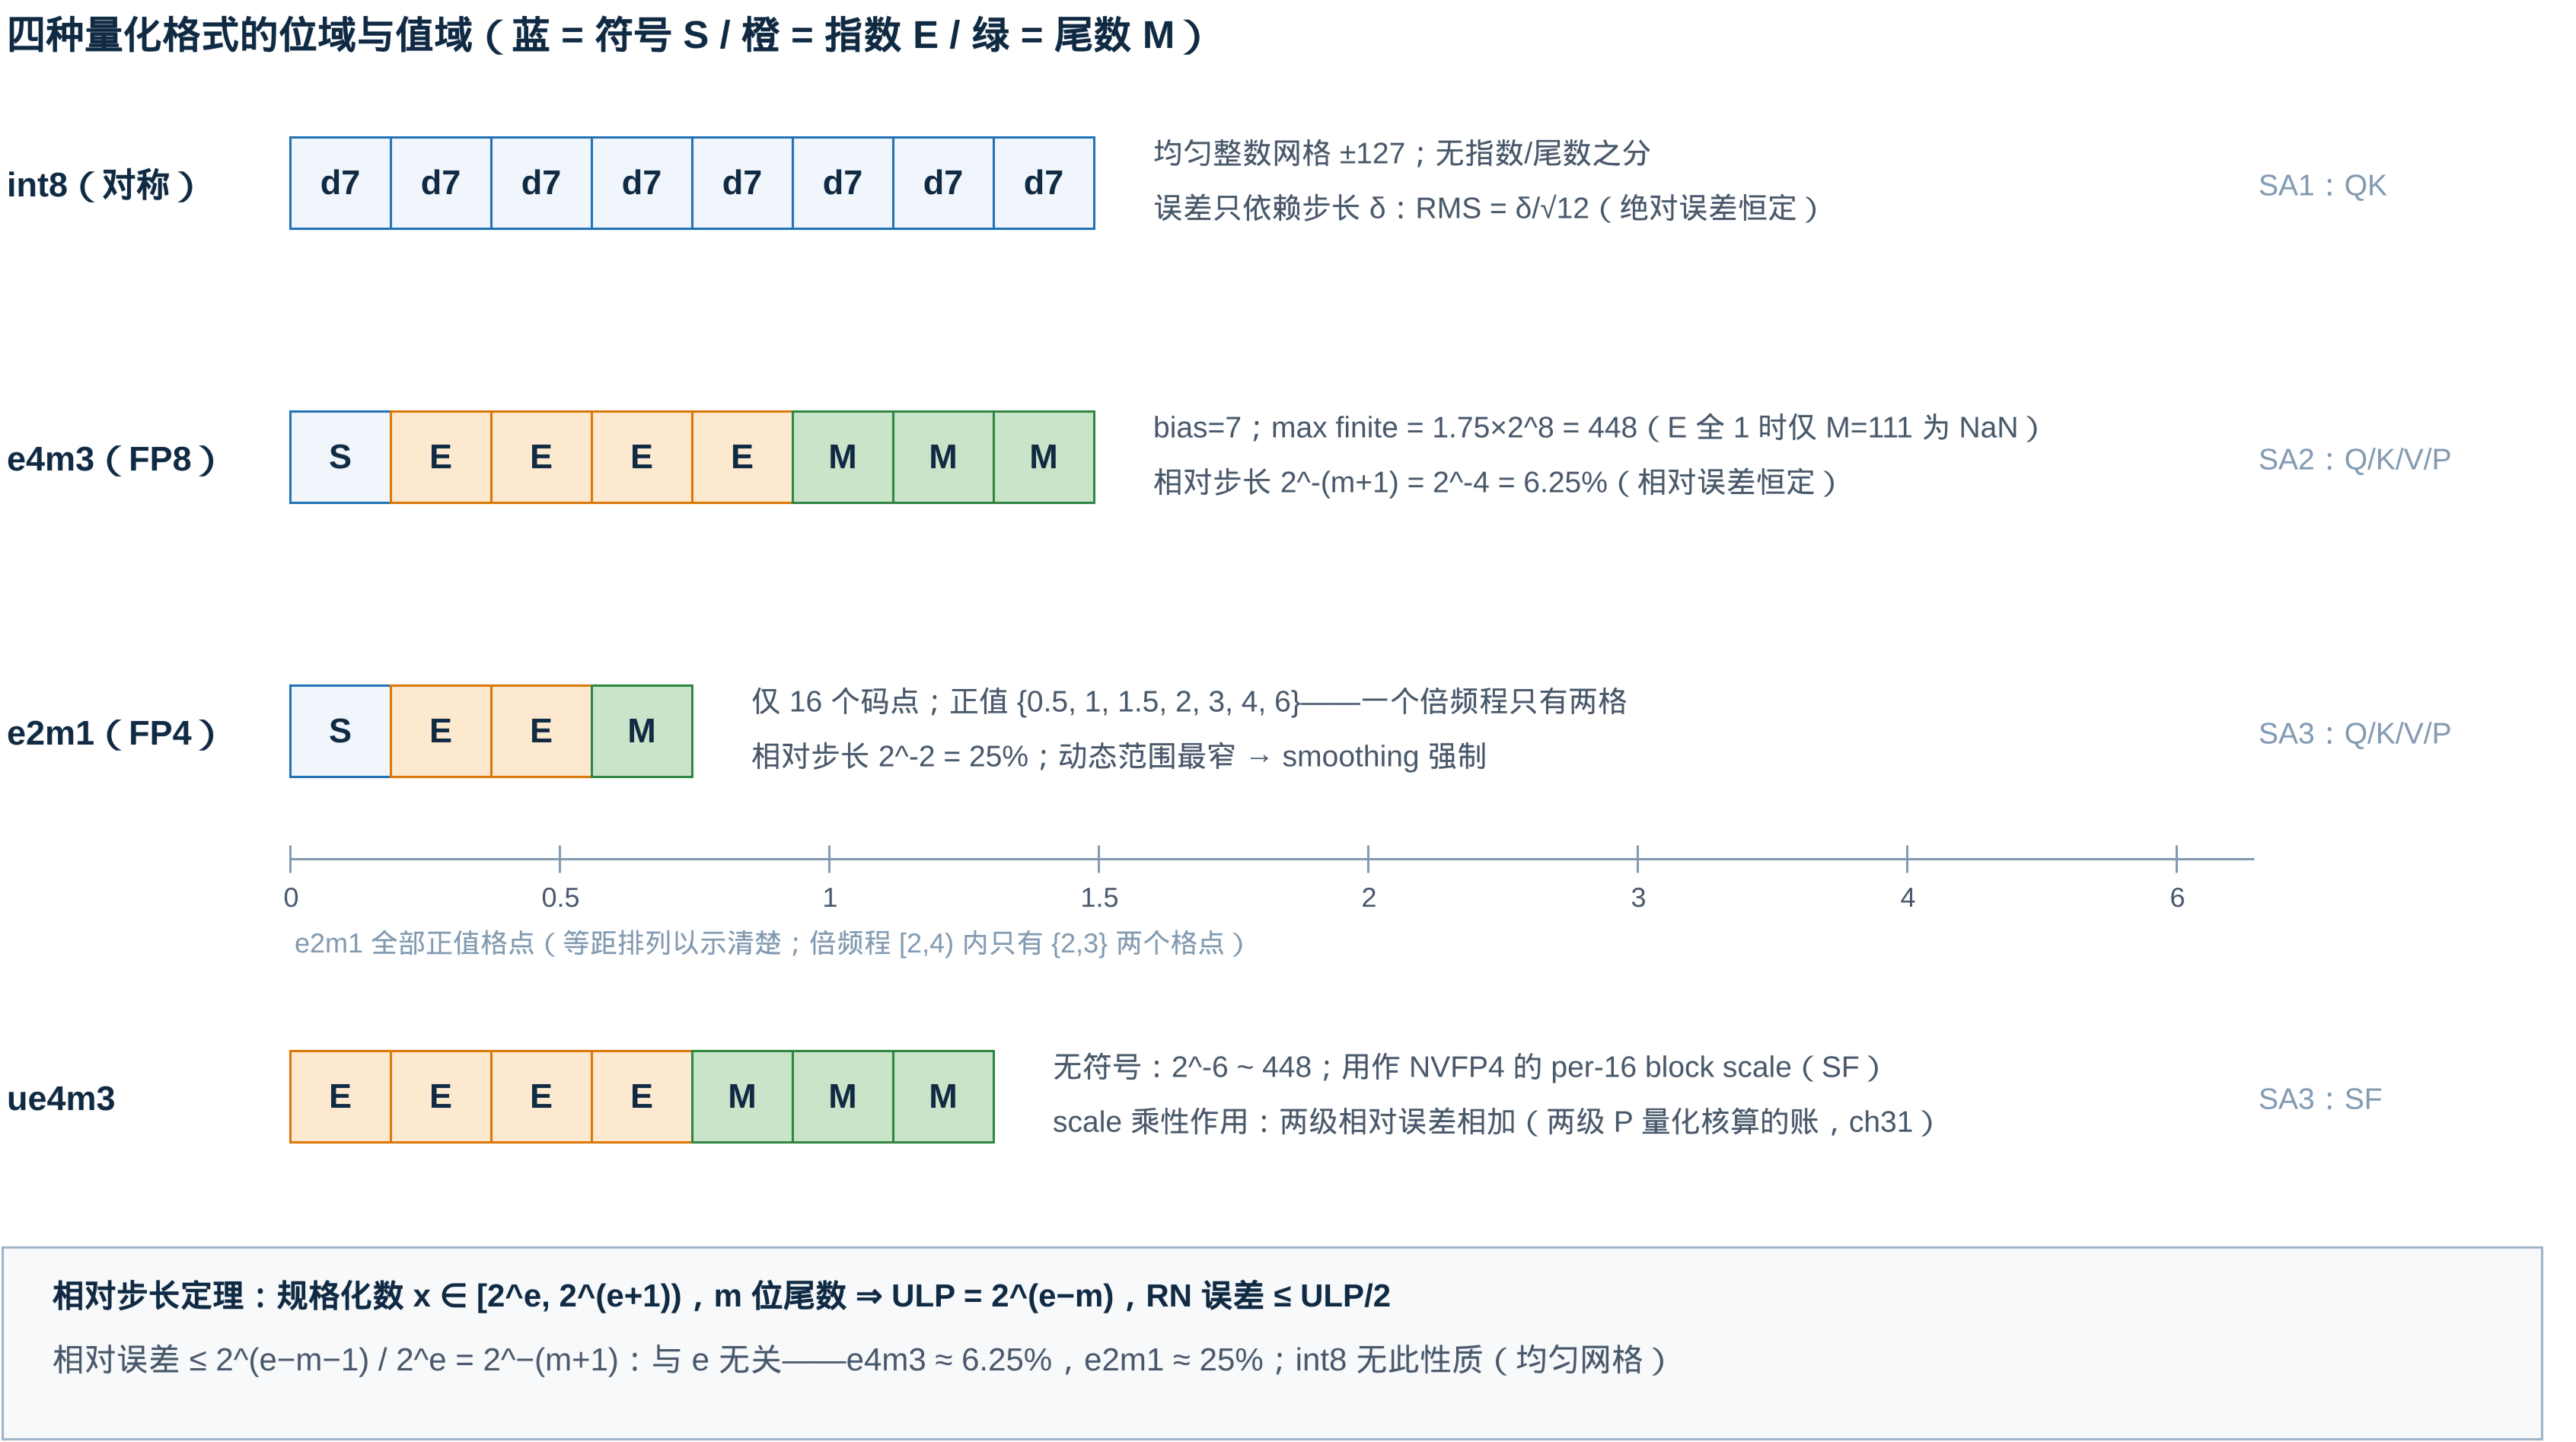
\includegraphics[width=0.92\textwidth]{figures/drawio/fig-27-1-fp-bitfield/fig-27-1-fp-bitfield.png}
  \begin{tikzpicture}[font=\tiny, >=Stealth,
    rl/.style={anchor=east, font=\bfseries\fontsize{4.8}{5.4}\selectfont, inner sep=1pt},
    bc/.style={draw, align=center, inner sep=1pt, minimum width=0.62cm,
      minimum height=0.50cm, font=\bfseries\fontsize{4.6}{5.2}\selectfont},
    an/.style={anchor=west, align=left, inner sep=1pt,
      font=\fontsize{4.2}{5.4}\selectfont, text width=6.60cm},
    sa/.style={anchor=west, font=\fontsize{4.2}{4.8}\selectfont, inner sep=1pt},
  ]
    % int8：均匀整数网格（8 位同权，无 S/E/M 之分）
    \node[rl] at (1.85,-0.29) {int8（对称）};
    \foreach \bb in {0,...,7} {
      \pgfmathtruncatemacro{\dg}{7-\bb}
      \node[bc, draw=tkBlue, fill=tkFillBlue] at ({2.36+0.62*\bb},-0.29) {d\dg};
    }
    \node[an] at (7.15,-0.29)
      {均匀整数网格 $\pm 127$；无指数/尾数之分\\
       误差只依赖步长 $\delta$：RMS $=\delta/\sqrt{12}$（绝对误差恒定）};
    \node[sa] at (14.00,-0.29) {SA1：QK};
    % e4m3：1 符号 + 4 指数 + 3 尾数
    \node[rl] at (1.85,-1.16) {e4m3（FP8）};
    \node[bc, draw=tkBlue, fill=tkFillBlue] at (2.36,-1.16) {S};
    \foreach \bb in {0,...,3} {
      \node[bc, draw=tkOrange, fill=tkFillOrange] at ({2.98+0.62*\bb},-1.16) {E};
    }
    \foreach \bb in {0,...,2} {
      \node[bc, draw=tkGreen, fill=tkFillGreen] at ({5.46+0.62*\bb},-1.16) {M};
    }
    \node[an] at (7.15,-1.16)
      {bias$=7$；max finite $=1.75\times 2^8=448$（E 全 1 时仅 M$=111$ 为 NaN）\\
       相对误差上界 $2^{-(m+1)}=2^{-4}=6.25\%$};
    \node[sa] at (14.00,-1.16) {SA2：Q/K/V/P};
    % e2m1：1 符号 + 2 指数 + 1 尾数
    \node[rl] at (1.85,-2.03) {e2m1（FP4）};
    \node[bc, draw=tkBlue, fill=tkFillBlue] at (2.36,-2.03) {S};
    \foreach \bb in {0,...,1} {
      \node[bc, draw=tkOrange, fill=tkFillOrange] at ({2.98+0.62*\bb},-2.03) {E};
    }
    \node[bc, draw=tkRed, fill=tkFillRed] at (4.22,-2.03) {M};
    \node[an] at (7.15,-2.03)
      {仅 16 个码点；正值 $\{0.5, 1, 1.5, 2, 3, 4, 6\}$——一个倍频程只有两格\\
       \textcolor{tkRed}{规格化域相对误差 $\le 25\%$；非规格化区无统一相对上界}};
    % e2m1 全部正值格点（等距排列；注明非等比）
    \draw[gray!70, thin] (2.05,-2.75) -- (14.40,-2.75);
    \foreach \bb in {0,...,7} {
      \pgfmathsetmacro{\xv}{2.05+1.764*\bb}
      \draw[gray!70, thin] (\xv,-2.81) -- (\xv,-2.69);
    }
    \node[align=center, font=\fontsize{4}{4.5}\selectfont, inner sep=1pt] at (2.05,-2.90) {0};
    \node[align=center, font=\fontsize{4}{4.5}\selectfont, inner sep=1pt] at (3.81,-2.90) {0.5};
    \node[align=center, font=\fontsize{4}{4.5}\selectfont, inner sep=1pt] at (5.58,-2.90) {1};
    \node[align=center, font=\fontsize{4}{4.5}\selectfont, inner sep=1pt] at (7.34,-2.90) {1.5};
    \node[align=center, font=\fontsize{4}{4.5}\selectfont, inner sep=1pt] at (9.10,-2.90) {2};
    \node[align=center, font=\fontsize{4}{4.5}\selectfont, inner sep=1pt] at (10.87,-2.90) {3};
    \node[align=center, font=\fontsize{4}{4.5}\selectfont, inner sep=1pt] at (12.63,-2.90) {4};
    \node[align=center, font=\fontsize{4}{4.5}\selectfont, inner sep=1pt] at (14.40,-2.90) {6};
    \node[an] at (2.05,-3.16)
      {e2m1 全部正值格点（等距排列以示清楚；倍频程 $[2,4)$ 内只有 $\{2,3\}$ 两个格点）};
    % ue4m3：无符号，4 指数 + 3 尾数
    \node[rl] at (1.85,-3.59) {ue4m3};
    \foreach \bb in {0,...,3} {
      \node[bc, draw=tkOrange, fill=tkFillOrange] at ({2.36+0.62*\bb},-3.59) {E};
    }
    \foreach \bb in {0,...,2} {
      \node[bc, draw=tkGreen, fill=tkFillGreen] at ({4.84+0.62*\bb},-3.59) {M};
    }
    \node[an] at (7.15,-3.59)
      {无符号：$2^{-6} \sim 448$；用作 NVFP4 的 per-group (16) block scale（SF）\\
       \textcolor{tkOrange}{scale 乘性作用：两级相对误差相加（两级 P 量化核算见 ch31）}};
    \node[sa] at (14.00,-3.59) {SA3：SF};
    % 相对步长定理
    \node[draw=gray!60, fill=gray!10, align=left, inner sep=3pt,
      font=\fontsize{4.6}{5.2}\selectfont, text width=15.2cm] at (7.80,-4.85)
      {\textbf{相对误差上界定理：规格化数 $x \in [2^e, 2^{e+1})$，$m$ 位尾数 $\Rightarrow$
        ULP $= 2^{e-m}$，RN 误差 $\le$ ULP$/2$}\\
       相对误差 $\le 2^{e-m-1}/2^e = 2^{-(m+1)}$：与 $e$ 无关——%
       \textcolor{tkGreen}{e4m3 $\approx 6.25\%$}，\textcolor{tkRed}{e2m1 $\approx 25\%$}；%
       int8 无此性质（均匀网格）};
  \end{tikzpicture}
  \caption{四种量化格式的位域与值域对照（int8 / e4m3 / e2m1 / ue4m3）。e4m3 的
  指数全 1 时仅 $M{=}111$ 编码 NaN，故满量程 448；e2m1 正半轴的 8 个码点
  （0 与 7 个正值）在数轴上标出，负半轴镜像，共 16 个，直观呈现
  \textbf{一个倍频程内只有两格}。}
  \label{fig:27-1}
\end{figure}

\begin{figure}[H]
  \centering
  % was: 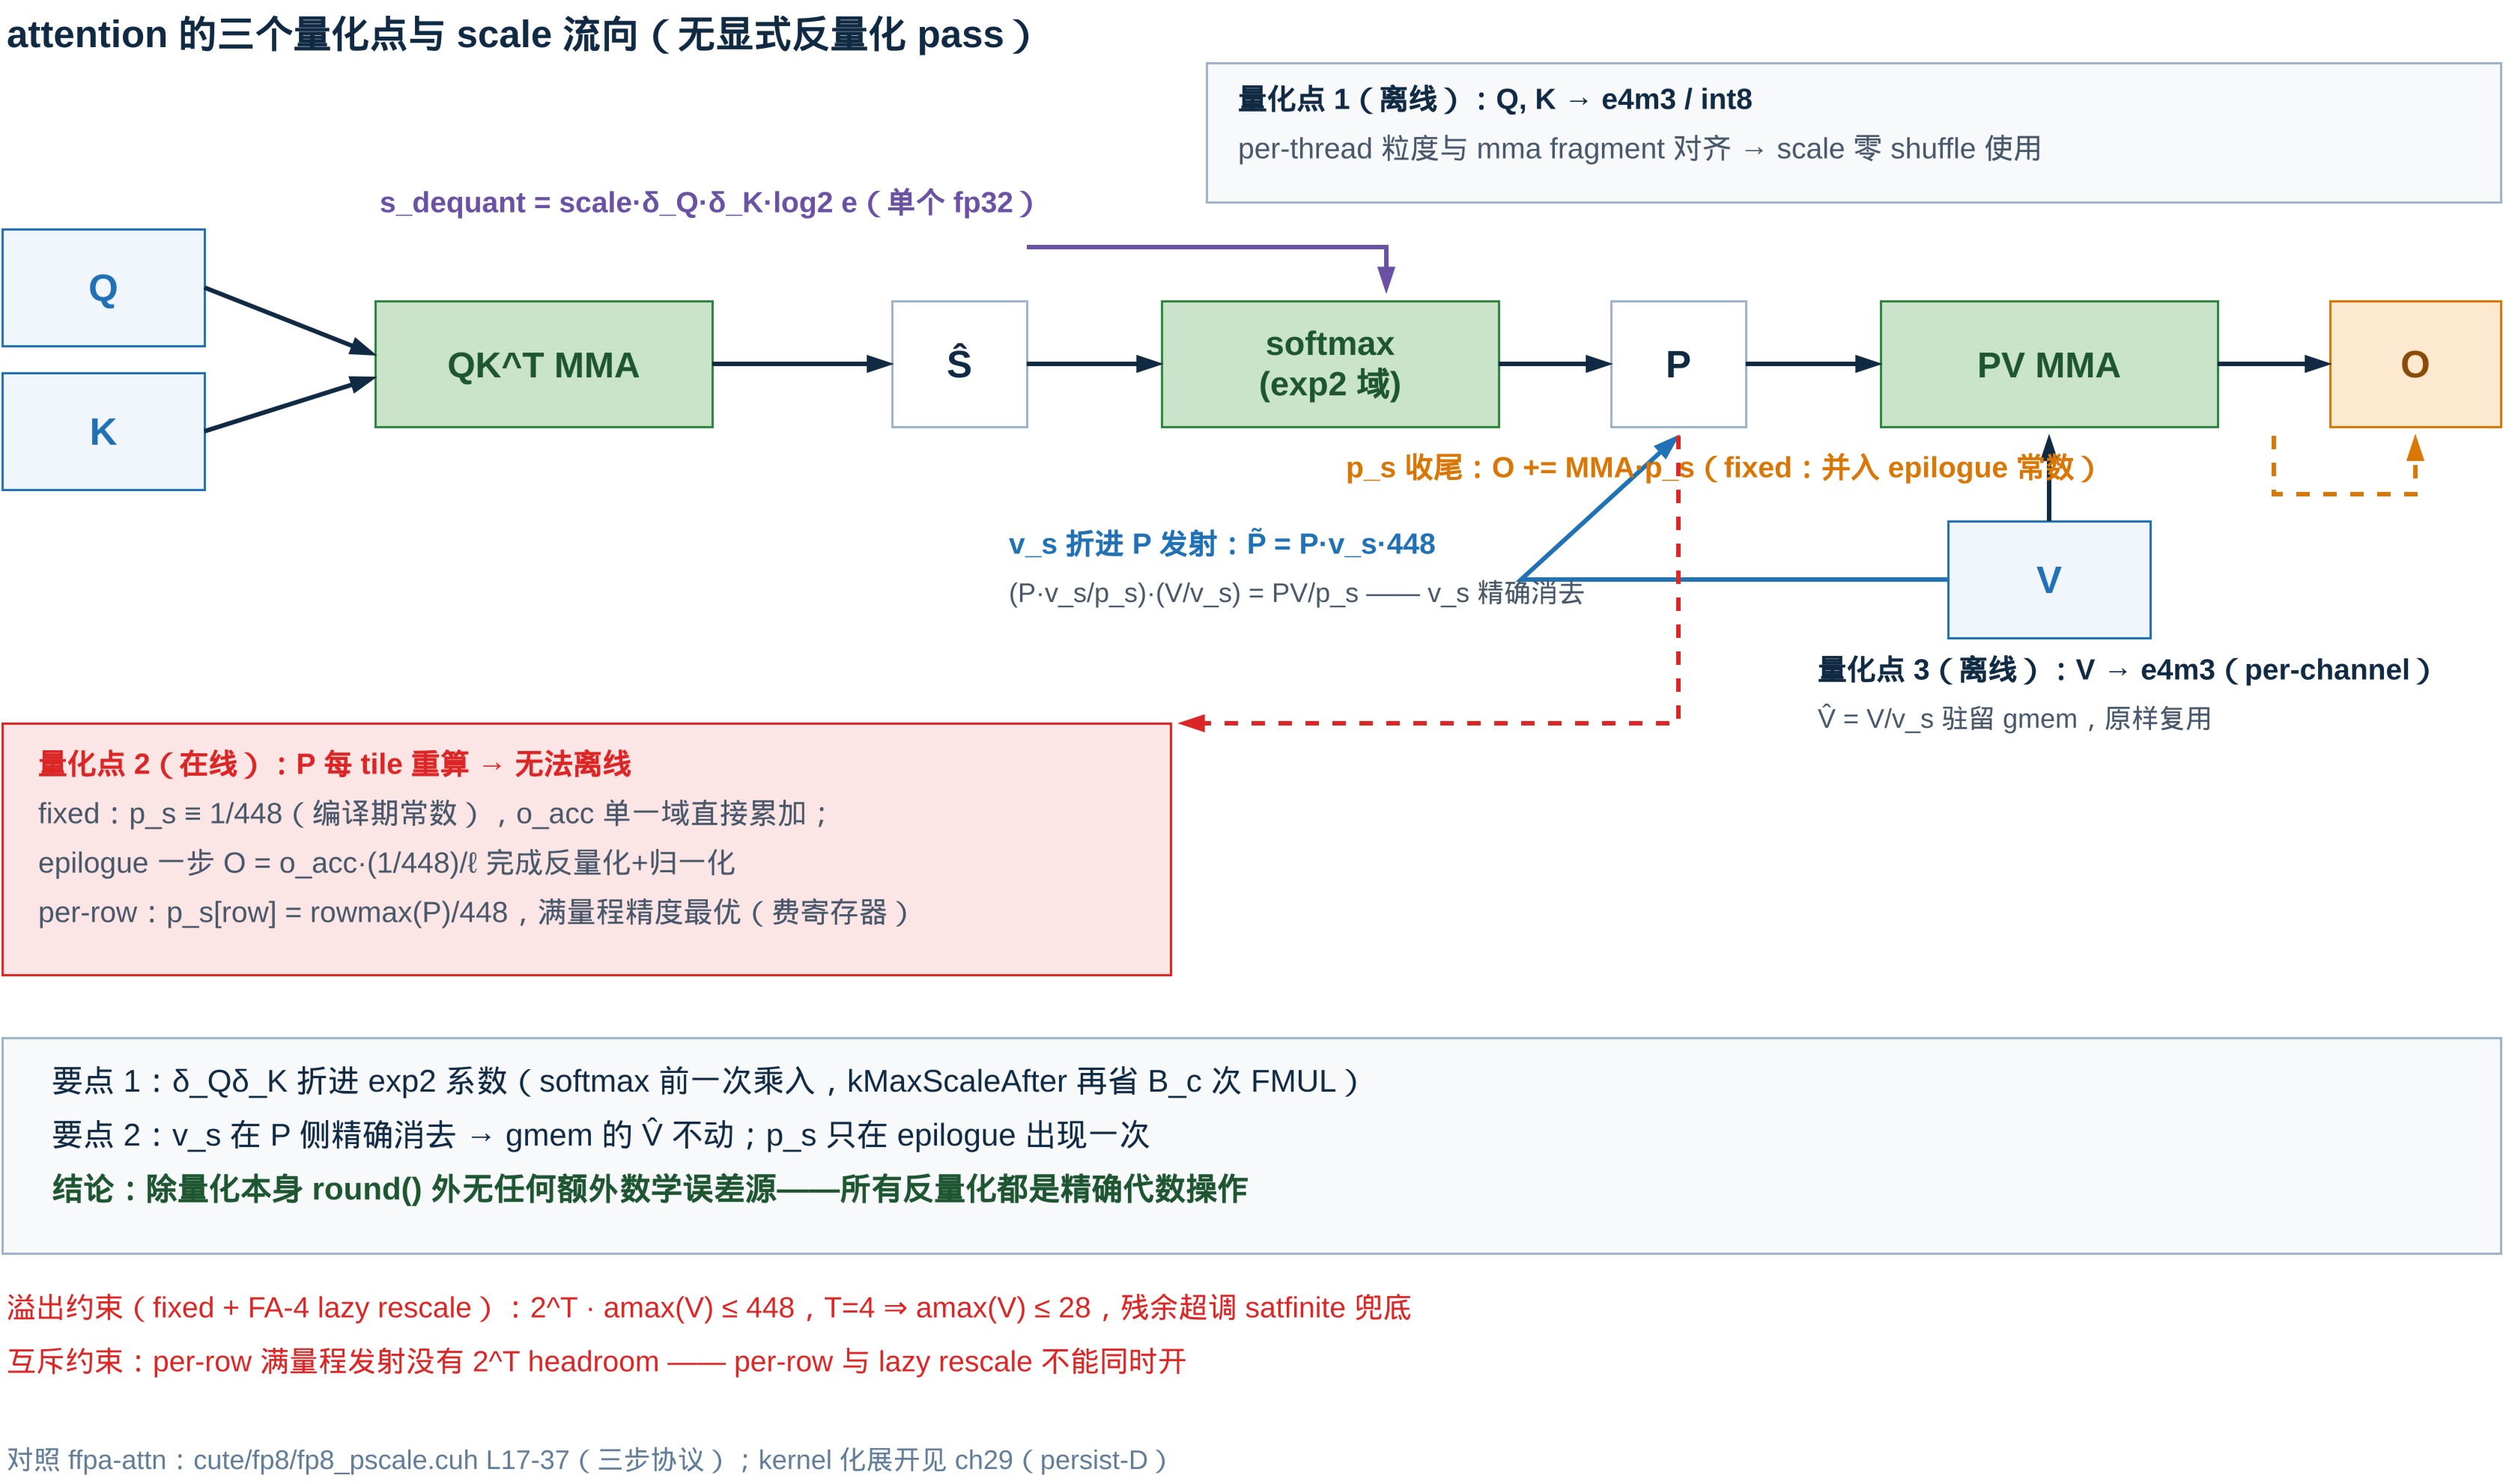
\includegraphics[width=0.95\textwidth]{figures/drawio/fig-27-2-quant-points/fig-27-2-quant-points.png}
  \begin{tikzpicture}[font=\tiny, >=Stealth,
    q/.style={draw=tkBlue, fill=tkFillBlue, text=tkBlue, align=center, inner sep=2pt,
      font=\bfseries\fontsize{5.4}{6}\selectfont},
    op/.style={draw=tkGreen, fill=tkFillGreen, text=tkGreen!75!black, align=center,
      inner sep=2pt, font=\bfseries\fontsize{4.6}{5.2}\selectfont},
    mid/.style={draw=gray!70, fill=white, align=center, inner sep=2pt,
      font=\bfseries\fontsize{5.4}{6}\selectfont},
    lit/.style={anchor=west, align=left, inner sep=1pt,
      font=\fontsize{4.2}{4.8}\selectfont},
    note/.style={anchor=west, align=left, inner sep=1pt,
      font=\fontsize{4.2}{4.8}\selectfont},
  ]
    % 主链：Q/K -> QK^T MMA -> S -> softmax -> P -> PV MMA -> O
    \node[q, text width=0.75cm] at (0.475,0.85) {Q};
    \node[q, text width=0.75cm] at (0.475,-0.35) {K};
    \node[op, text width=1.35cm] at (2.35,0.25) {QK$^{\top}$ MMA};
    \node[mid] at (4.125,0.25) {$\hat{S}$};
    \node[op, text width=1.35cm] at (5.90,0.25) {softmax\\(exp2 域)};
    \node[mid] at (7.675,0.25) {P};
    \node[op, text width=1.35cm] at (9.45,0.25) {PV MMA};
    \node[draw=tkOrange, fill=tkFillOrange, text=tkOrange!80!black, align=center,
      inner sep=2pt, font=\bfseries\fontsize{5.4}{6}\selectfont] at (11.30,0.25) {O};
    \draw[->, gray!80, semithick] (0.98,0.85) -- (1.52,0.46);
    \draw[->, gray!80, semithick] (0.98,-0.35) -- (1.52,0.06);
    \draw[->, gray!80, semithick] (3.17,0.25) -- (3.71,0.25);
    \draw[->, gray!80, semithick] (4.54,0.25) -- (5.06,0.25);
    \draw[->, gray!80, semithick] (6.74,0.25) -- (7.26,0.25);
    \draw[->, gray!80, semithick] (8.09,0.25) -- (8.61,0.25);
    \draw[->, gray!80, semithick] (10.29,0.25) -- (10.81,0.25);
    \node[q, text width=0.75cm] at (9.55,-1.05) {V};
    \draw[->, gray!80, semithick] (9.55,-0.72) -- (9.55,-0.09);
    % 量化点 1（离线 Q/K）
    \node[draw=gray!60, fill=gray!10, align=left, inner sep=3pt,
      font=\fontsize{4.4}{5}\selectfont, text width=7.6cm] at (11.00,1.72)
      {\textbf{量化点 1（离线）：Q, K $\to$ e4m3 / int8}\\
       per-thread 粒度与 mma fragment 对齐 $\to$ scale 零 shuffle 使用};
    % scale 流 1：delta_Q*delta_K 折进 exp2 系数
    \draw[->, tkPurple, semithick] (4.54,0.95) -- (5.90,0.95) -- (5.90,0.60);
    \node[lit, text=tkPurple] at (1.55,1.14)
      {$s_{\mathrm{dequant}} = \mathrm{scale}\cdot\delta_Q\delta_K\cdot\log_2 e$（单个 fp32）};
    % scale 流 2：v_s 折进 P 发射（V 的左侧），及量化点 3
    \draw[->, tkBlue, semithick] (9.55,-0.78) -- (7.90,-0.78) -- (7.90,-0.12);
    \node[lit, text=tkBlue] at (2.95,-1.02) {$v_s$ 折进 P 发射：$\tilde{P} = P\cdot v_s\cdot 448$};
    \node[lit] at (2.95,-1.30)
      {$(P\cdot v_s/p_s)\cdot(V/v_s) = PV/p_s$ —— 未舍入代数中 $v_s$ 精确消去};
    \node[lit, text=tkOrange!80!black] at (10.35,-1.05)
      {\textbf{量化点 3（离线）：V $\to$ e4m3（per-channel）}};
    \node[lit] at (10.35,-1.32) {$\hat{V} = V/v_s$ 驻留 gmem，原样复用};
    % scale 流 3：p_s 在 epilogue 收尾
    \draw[->, dashed, tkOrange, semithick]
      (11.05,-0.18) -- (11.05,-0.72) -- (11.75,-0.72) -- (11.75,-0.18);
    \node[lit, text=tkOrange!80!black] at (8.15,-0.45)
      {$p_s$ 收尾：$O \mathrel{+}=$ MMA$\cdot p_s$（fixed：并入 epilogue 常数）};
    % 量化点 2（在线 P）：每 tile 重算，无法离线
    \node[draw=tkRed, fill=tkFillRed, align=left, inner sep=3pt,
      font=\fontsize{4.2}{4.8}\selectfont, text width=7.5cm] at (4.00,-2.45)
      {\textbf{量化点 2（在线）：P 每 tile 重算 $\to$ 无法离线}\\
       fixed：$p_s \equiv 1/448$（编译期常数），o\_acc 单一域直接累加；\\
       epilogue 一步 $O = o\_acc\cdot(1/448)/\ell$ 完成反量化 $+$ 归一化\\
       per-row：$p_s[\mathrm{row}] = \mathrm{rowmax}(P)/448$，满量程精度最优（多占寄存器）};
    \draw[->, dashed, tkRed, semithick] (7.65,-0.05) -- (7.65,-1.80);
    % 底部要点与约束
    \node[draw=gray!60, fill=gray!10, align=left, inner sep=3pt,
      font=\fontsize{4.4}{5}\selectfont, text width=14.8cm] at (7.60,-3.90)
      {要点 1：$\delta_Q\delta_K$ 折进 exp2 系数（per-block 下 kMaxScaleAfter 再省 $B_c$ 次 FMUL）\\
       要点 2：$v_s$ 在未舍入代数中精确消去 $\to$ gmem 的 $\hat{V}$ 不动；$p_s$ 只在 epilogue 出现一次\\
       \textbf{\textcolor{tkGreen}{结论：实数代数下除 round() 外无额外误差源；浮点执行仍有乘加、exp2 与累加舍入}}};
    \node[note, text=tkRed] at (0.10,-4.72)
      {溢出约束（fixed $+$ FA-4 lazy rescale）：$2^T\cdot\mathrm{amax}(V) \le 448$，%
       $T=4 \Rightarrow \mathrm{amax}(V) \le 28$，残余超调 satfinite 兜底};
    \node[note, text=tkRed] at (0.10,-4.98)
      {互斥约束：per-row 满量程发射没有 $2^T$ headroom —— per-row 与 lazy rescale 不能同时开};
    \node[note, text=gray!80!black] at (0.10,-5.32)
      {对照 ffpa-attn：cute/fp8/fp8\_pscale.cuh L17-37（三步协议）；kernel 化展开见 ch29（persist-D）};
  \end{tikzpicture}
  \caption{attention 的三个量化点与 scale 流向：$\delta_Q\delta_K$ 折进 exp2
  系数（式~\ref{eq:27-qk-fold}）、$v_s$ 在未舍入代数中精确消去
  （式~\ref{eq:27-vs-cancel}）、$p_{scale}$ 在 epilogue 一步收尾。}
  \label{fig:27-2}
\end{figure}

\begin{figure}[H]
  \centering
  % was: 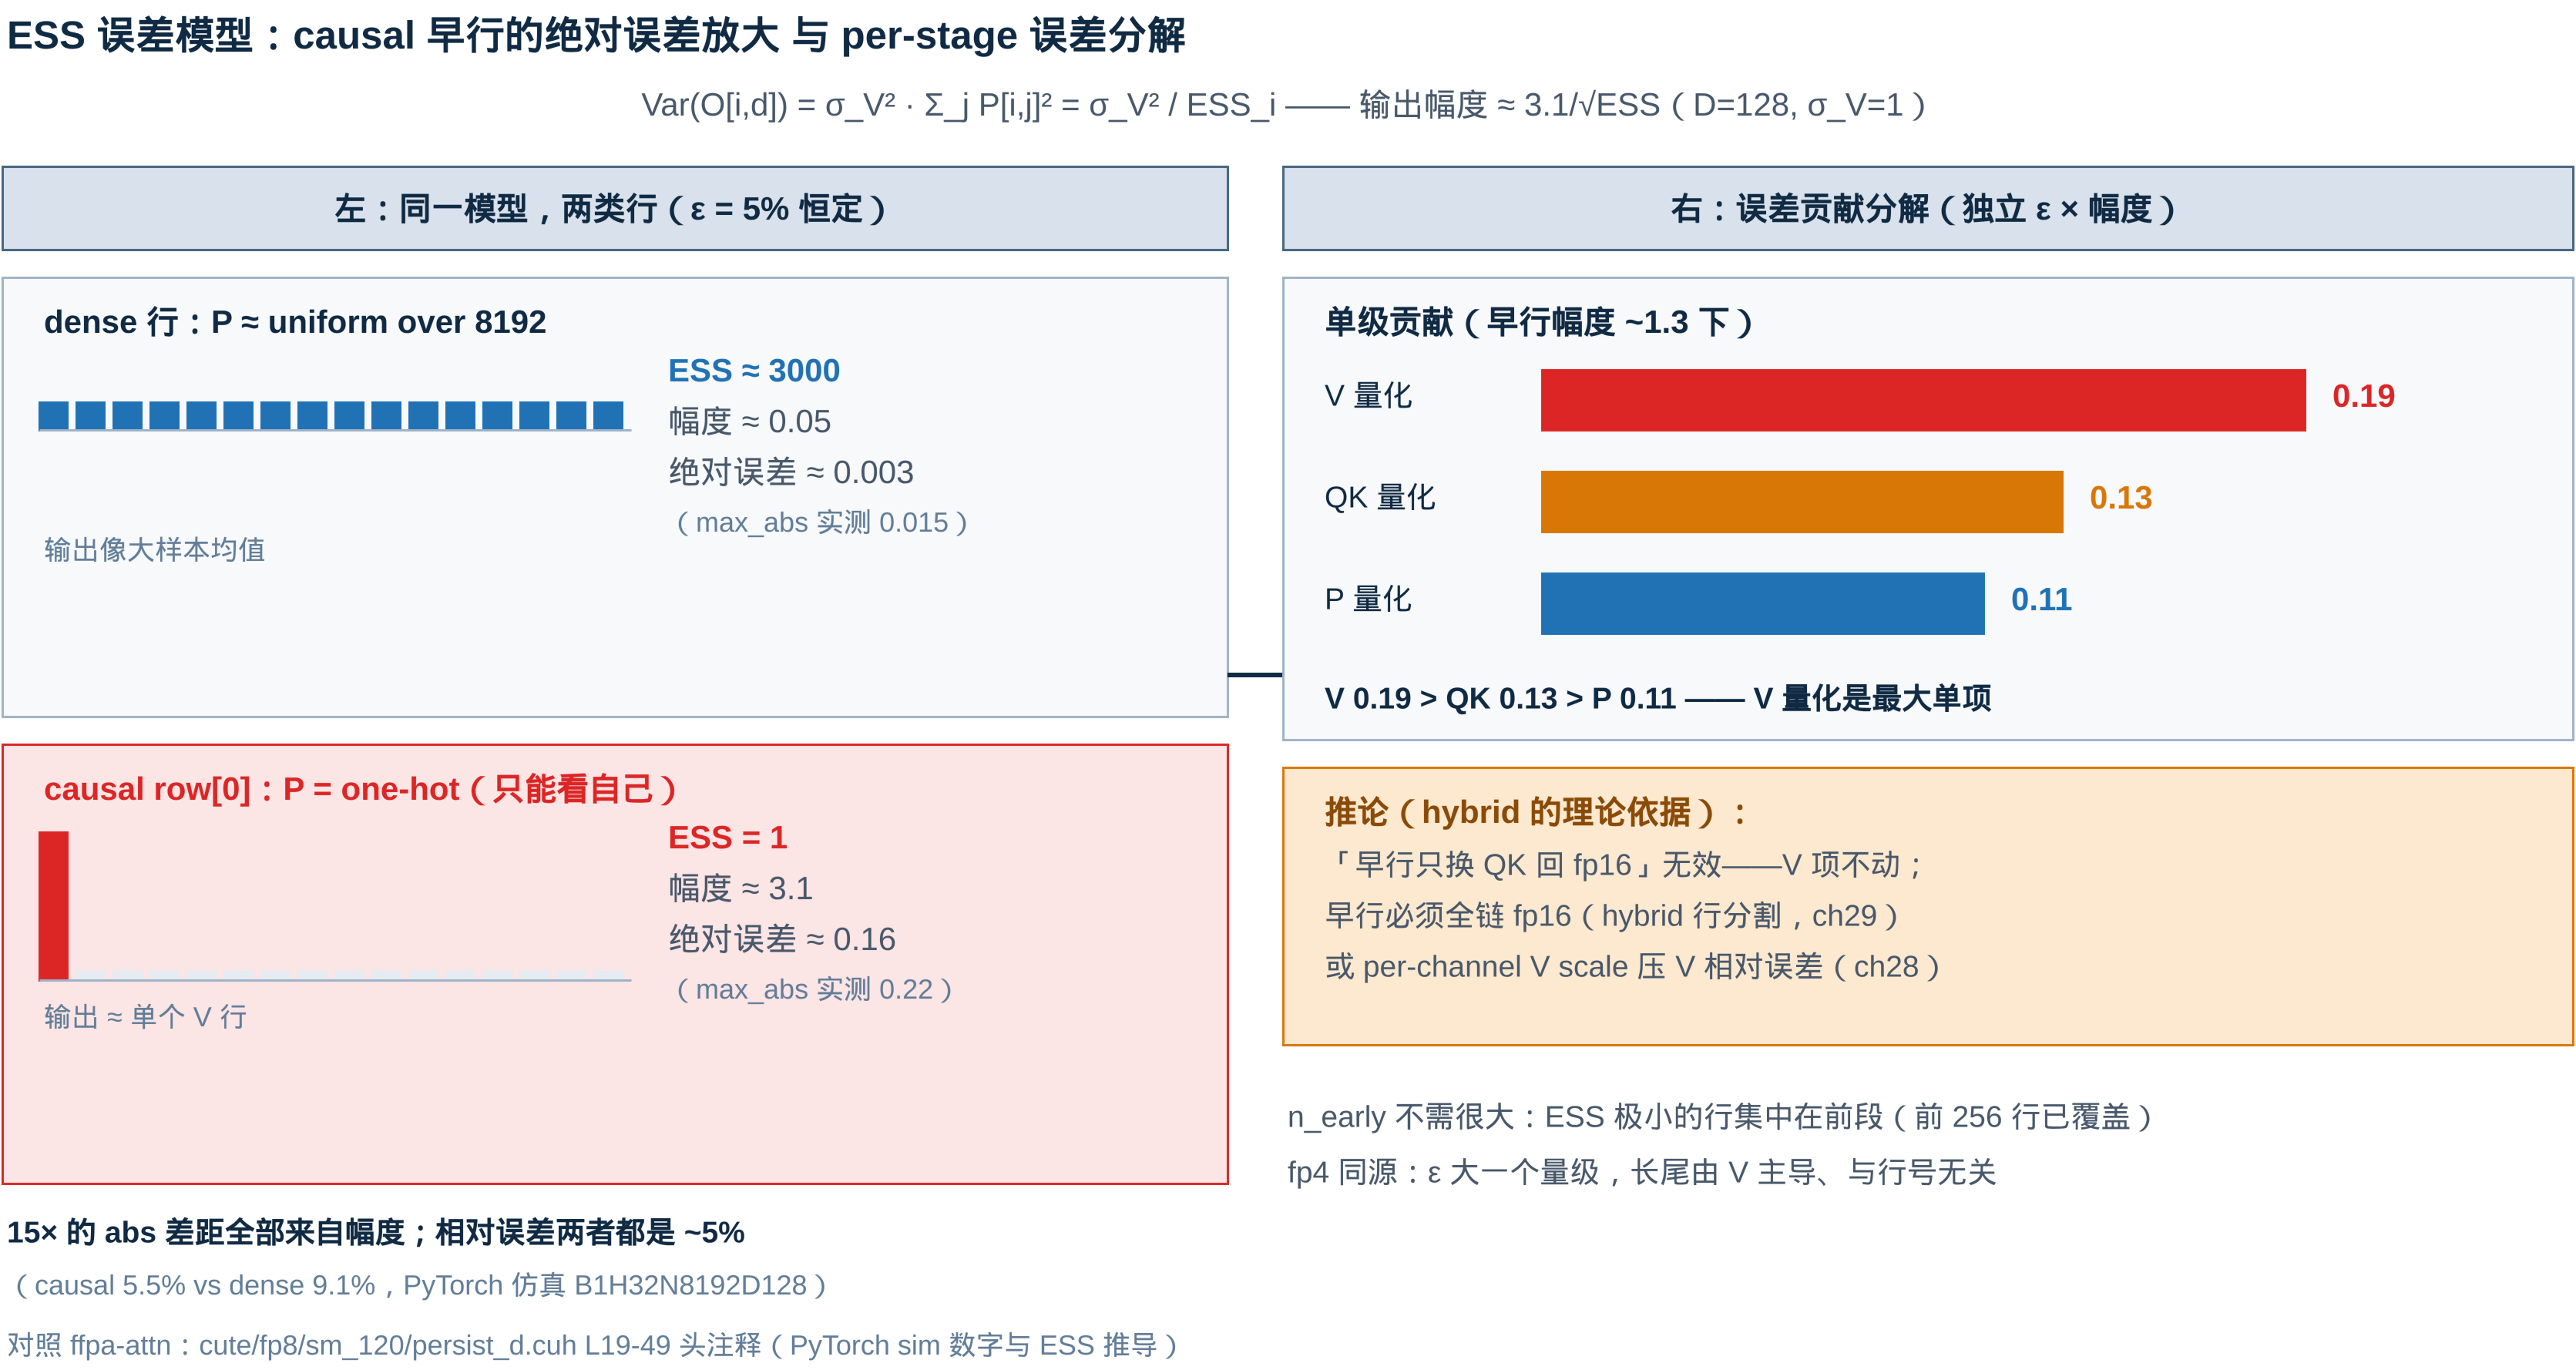
\includegraphics[width=0.9\textwidth]{figures/drawio/fig-27-3-ess-decompose/fig-27-3-ess-decompose.png}
  \begin{tikzpicture}[font=\tiny, >=Stealth,
    hd/.style={align=center, inner sep=2pt, font=\bfseries\fontsize{4.6}{5.2}\selectfont},
    card/.style={draw=gray!55, fill=gray!8},
    tl/.style={anchor=west, align=left, inner sep=1pt,
      font=\fontsize{4.4}{5}\selectfont},
    ax/.style={anchor=west, align=left, inner sep=1pt,
      font=\fontsize{4.2}{4.8}\selectfont},
  ]
    % 左半：dense 行与 causal 早行（同一 ε 下幅度差异）
    \node[hd, fill=gray!16, text width=7.10cm] at (3.70,-0.20)
      {左：同一模型，两类行（$\varepsilon = 5\%$ 恒定）};
    \draw[card] (0.15,-0.45) rectangle (7.25,-2.60);
    \node[tl, font=\bfseries\fontsize{4.6}{5.2}\selectfont] at (0.30,-0.62)
      {dense 行：P 非均匀，但 ESS 较大};
    \foreach \bb in {0,...,15} {
      \pgfmathsetmacro{\xb}{0.30+0.16*\bb}
      \pgfmathsetmacro{\hh}{0.10+0.20*mod(5*\bb+1,7)/6}
      \fill[tkBlue] (\xb,-1.95) rectangle ({\xb+0.12},{-1.95+\hh});
    }
    \draw[gray!60, thin] (0.30,-1.95) -- (2.86,-1.95);
    \node[tl, text=tkBlue, font=\bfseries\fontsize{4.6}{5.2}\selectfont] at (3.20,-0.95)
      {ESS $\approx$ 3000};
    \node[tl] at (3.20,-1.20) {幅度 $\approx$ 0.05};
    \node[tl] at (3.20,-1.45) {绝对误差 $\approx$ 0.003};
    \node[tl, text=gray!80!black] at (3.20,-1.70) {（max\_abs 实测 0.015）};
    \node[tl, text=gray!80!black] at (0.30,-2.28) {输出像大样本均值};
    \draw[card, draw=tkRed, fill=tkFillRed] (0.15,-2.80) rectangle (7.25,-5.20);
    \node[tl, text=tkRed, font=\bfseries\fontsize{4.6}{5.2}\selectfont] at (0.30,-2.97)
      {causal row[0]：P $=$ one-hot（只能看自己）};
    \foreach \bb in {0,...,15} {
      \pgfmathsetmacro{\xb}{0.30+0.16*\bb}
      \pgfmathsetmacro{\hh}{\bb == 0 ? 1.15 : 0.07}
      \ifnum\bb=0
        \fill[tkRed] (\xb,-4.55) rectangle ({\xb+0.12},{-4.55+\hh});
      \else
        \fill[gray!40] (\xb,-4.55) rectangle ({\xb+0.12},{-4.55+\hh});
      \fi
    }
    \draw[gray!60, thin] (0.30,-4.55) -- (2.86,-4.55);
    \node[tl, text=tkRed, font=\bfseries\fontsize{4.6}{5.2}\selectfont] at (3.20,-3.55)
      {ESS $=$ 1};
    \node[tl] at (3.20,-3.80) {幅度 $\approx$ 3.1};
    \node[tl] at (3.20,-4.05) {绝对误差 $\approx$ 0.16};
    \node[tl, text=gray!80!black] at (3.20,-4.30) {（max\_abs 实测 0.22）};
    \node[tl, text=gray!80!black] at (0.30,-4.88) {输出 $\approx$ 单个 V 行};
    \node[tl, font=\bfseries\fontsize{4.6}{5.2}\selectfont] at (0.25,-5.45)
      {$15\times$ 的 abs 差距主要来自早行幅度；相对误差同量级（causal 5.5\% vs dense 9.1\%，并不相等）};
    \node[tl, text=gray!80!black] at (0.25,-5.72)
      {（causal 5.5\% vs dense 9.1\%，PyTorch 仿真 B1H32N8192D128）};
    % 右半：per-stage 误差贡献（单级 ε × 幅度）
    \node[hd, fill=gray!16, text width=7.60cm] at (11.60,-0.20)
      {右：误差贡献分解（独立 $\varepsilon \times$ 幅度）};
    \draw[card] (7.80,-0.45) rectangle (15.40,-2.60);
    \node[tl, font=\bfseries\fontsize{4.6}{5.2}\selectfont] at (7.95,-0.62)
      {单级贡献（早行幅度 $\sim$3.1 下）};
    \node[ax] at (7.95,-0.95) {V 量化};
    \fill[tkRed] (9.15,-1.07) rectangle (13.15,-0.83);
    \node[ax, text=tkRed, font=\bfseries\fontsize{4.6}{5.2}\selectfont] at (13.25,-0.95) {0.19};
    \node[ax] at (7.95,-1.35) {QK 量化};
    \fill[tkOrange] (9.15,-1.47) rectangle (11.89,-1.23);
    \node[ax, text=tkOrange!80!black, font=\bfseries\fontsize{4.6}{5.2}\selectfont] at (11.99,-1.35) {0.13};
    \node[ax] at (7.95,-1.75) {P 量化};
    \fill[tkBlue] (9.15,-1.87) rectangle (11.47,-1.63);
    \node[ax, text=tkBlue, font=\bfseries\fontsize{4.6}{5.2}\selectfont] at (11.57,-1.75) {0.11};
    \node[tl, font=\bfseries\fontsize{4.6}{5.2}\selectfont] at (7.95,-2.20)
      {V 0.19 $>$ QK 0.13 $>$ P 0.11 —— V 量化是最大单项};
    \node[draw=tkOrange, fill=tkFillOrange, align=left, inner sep=3pt,
      font=\fontsize{4.4}{5}\selectfont, text width=7.30cm] at (11.60,-3.30)
      {\textbf{\textcolor{tkOrange!70!black}{推论（hybrid 的理论依据）：}}\\
       \textbf{早行只换 QK 回 fp16}不能消除主导误差——V 项不动；\\
       可选全链 fp16（hybrid 行分割，ch29）\\
       或 per-channel V scale 压 V 相对误差（ch28）};
    \node[ax] at (7.85,-4.75) {n\_early 不需很大：ESS 极小的行集中在前段（前 256 行已覆盖）};
    \node[ax] at (7.85,-5.00) {fp4 同源：$\varepsilon$ 大一个量级，长尾由 V 主导、与行号无关};
    \node[ax, text=gray!80!black] at (0.25,-6.05)
      {对照 ffpa-attn：cute/fp8/sm\_120/persist\_d.cuh L19-49 头注释（PyTorch sim 数字与 ESS 推导）};
  \end{tikzpicture}
  \caption{ESS 误差模型与 per-stage 误差分解：左半为 dense 行与 causal 早行的
  $P$ 分布/ESS/幅度对比（表~\ref{tab:27-ess} 的图形化），右半为
  V $>$ QK $>$ P 的误差贡献分解，以及全链 fp16 与 per-channel V 两条修正路径。}
  \label{fig:27-3}
\end{figure}

\section{性能分析}

量化的收益上限由 27.2.1 的精度阶梯给出。实际达成率取决于两个非理想因素：
量化前处理链的开销（第~\ref{ch:28}~章：kv\_mean / quantize / 转置链的
带宽需求，理想情况可用满 HBM 带宽、E2E 占比个位数百分比）与 softmax/CVT 等
非 MMA 指令的占比（第~\ref{ch:29}~章：persist-D 的流水线设计让 tensor pipe 占比
达 $\sim$77\%）。本机（RTX PRO 5000 72GB Blackwell，sm\_120）以
\texttt{ffpa\_attn.bench} 实测 fp8 路径基线：
\begin{lstlisting}[style=console]
$ FFPA_CUDA_ALLOW_SMALL_D=1 CUDA_VISIBLE_DEVICES=7 \
  python -m ffpa_attn.bench --fwd-backend cuda --cuda-impl fp8 \
  --tasks self-attn --D 128 --no-bwd --show-allclose
| self-attn | fp16 | 8192/8192 | allclose OK | 3.01 / 5.12 ms | 365T / 215T | 1.70x |
\end{lstlisting}
fp8 全链（含前处理）相对 SDPA fp16 加速 $1.70\times$，折合 365 TFLOPS
（同形状 fp16 kernel 的两倍量级，与 e4m3 吞吐阶梯一致）。D 与任务维度的完整
矩阵、knob 扫描与 5090 对照见第~\ref{ch:33}~章。

\section{实践经验}

\begin{itemize}[itemsep=2pt,topsep=2pt]
  \item \textbf{先定发射域，再写 kernel}：fp8/fp4 kernel 的第一份设计草图应该是
        每个 fragment 生命周期的值域区间图（$P \cdot v_s \cdot 448 \cdot
        2^{\tau}$ 类推），所有格式选择从这张图反推，本章 27.3.4--27.3.6 的顺序
        即是如此。
  \item \textbf{粒度对齐 fragment 是零成本精度}：per-thread/per-channel 的收益
        不止于更细的粒度：scale 恰好落在每 lane 私有或每行常数的零开销位置
        （式~\ref{eq:27-qk-fold} 折叠的前提）。
  \item \textbf{误差分析要分幅度与相对两层}：见到 causal 精度差 15 倍时，先查
        相对误差是否一致（式~\ref{eq:27-ess} 的 ESS 口径），再决定是降
        $\varepsilon$ 还是分割行。
\end{itemize}

\section{常见坑}

\begin{enumerate}[itemsep=2pt,topsep=2pt]
  \item \textbf{全零块的 $0/0$ NaN}：$\mathrm{amax} = 0 \Rightarrow \delta = 0$，
        式~\ref{eq:27-quant-op} 的除法产生 NaN。fp4 路径对 SF 域显式防护
        （$\mathrm{SF} = 0 \Rightarrow \mathrm{SF}^{-1} = 0$）；fp8 的
        per-row $p_{scale}$ 同样带零检查（27.4~节）。head\_dim padding 列
        是全零块最常见的来源。
  \item \textbf{per-row 满量程 + lazy rescale = 溢出}：满量程发射没有 $2^{\tau}$
        的 headroom（式~\ref{eq:27-overflow}），两者互斥是硬约束不是调参问题。
  \item \textbf{把 satfinite 当正确性保证}：satfinite 只是钳位，被钳的值已携带
        不可控误差；它的作用是钳住残余超调（$\mathrm{amax}(V)$ 刚好越过 28
        的边缘 case），不是精度修正手段。
  \item \textbf{混淆 fp16 家族与 fp8 家族的 $\tau$}：FA-4 对 BF16 取 $\tau = 8$
        （$2^8 = 256$ 在 fp16 域安全），fp8 发射域取 $T = 4$。跨家族直接沿用阈值会
        超出 e4m3 上限。
  \item \textbf{引用行号漂移}：ffpa-attn 是活跃仓库，本章行号锚定 commit
        \texttt{861d75e}（附录~\ref{app:D}）；升级仓库后需复核
        （\texttt{grep -n} 三步协议首行 "Why P needs"）。
\end{enumerate}

\section{面试要点速查}

\begin{itemize}[itemsep=1pt,topsep=2pt]
  \item Q：e4m3 与 int8 量化误差的本质区别？\\
        A：均匀网格与指数网格。int8 的绝对误差由量化步长决定；e4m3 在规格化域的
        相对误差上界为 $2^{-(m+1)}=6.25\%$（定理~\ref{thm:27-relstep}），
        非规格化区则没有统一的相对误差上界。值域横跨多倍频程用指数，
        幅度紧凑用均匀。
  \item Q：为什么 P 必须在线量化，Q/K/V 可以离线？\\
        A：Q/K/V 是前向输入侧的静态张量；P 每 tile 重算且依赖 softmax 状态，
        只能在寄存器 fragment 上就地量化（27.2.2）。
  \item Q：$v_s$ 如何消去？为什么 fold 进 P 而不是 V？\\
        A：$(P v_s / p_{scale}) \cdot (V / v_s) = PV / p_{scale}$ 在未舍入代数中精确成立
        （式~\ref{eq:27-vs-cancel}），量化舍入后乘积为近似；fold 进 P 侧使 gmem 的
        $\hat V$ 原样复用，无需重写。
  \item Q：fixed 与 per-row $p_{scale}$ 怎么选？\\
        A：fixed 编译期常数、单一累加域、可与 lazy rescale 组合，默认；per-row
        每行满量程精度最优，但要 rowmax 归约 + $o_{tile}$ 暂存 + 与 lazy rescale
        互斥（27.3.4）。
  \item Q：causal 前几行精度差 15 倍，是误差放大吗？\\
        A：绝对误差确实随输出幅度放大，但相对误差仍在同一量级（5.5\% vs 9.1\%，
        并非全行一致）。绝对误差 $= \varepsilon \times$ 幅度，早行 ESS 小、幅度大
        （式~\ref{eq:27-ess}）。可选 hybrid 全链 fp16 或降低 V 的相对误差；单换 QK
        不能消除主导的 V 误差（V 0.19 是最大单项）。
  \item Q：FA-4 lazy rescale 在量化域要额外考虑什么？\\
        A：发射值被 $2^{\tau}$ 膨胀，需核算格式上限
        $2^{\tau}\,\mathrm{amax}(V) \le 448$（式~\ref{eq:27-overflow}），
        fp8 取 $T{=}4$ 而非 BF16 的 8。
\end{itemize}

\section{最小测试与动手实验}

Part VI 不新增 \texttt{book/tests}，验证链路统一为 \texttt{ffpa\_attn.bench} CLI
（ffpa-attn 0.2.5.dev25 editable 安装，本机 PRO 5000，卡位 7）。本章实验只覆盖
fp8 基线口径：

\begin{lstlisting}[style=console]
# 前置：conda activate cdit；D<=256 需放开 small-D 门禁
$ export FFPA_CUDA_ALLOW_SMALL_D=1 CUDA_VISIBLE_DEVICES=7

# 实验 1：fp8 基线（self-attn D128，对照 SDPA，验证 allclose）
$ python -m ffpa_attn.bench --fwd-backend cuda --cuda-impl fp8 \
    --tasks self-attn --D 128 --no-bwd --show-allclose
# 预期：allclose 列 OK；speedup ~1.7x（365T vs 215T，本机 PRO 5000）

# 实验 2：fp4 同形状对照（e2m1 的精度与速度差）
$ python -m ffpa_attn.bench --fwd-backend cuda --cuda-impl fp4 \
    --tasks self-attn --D 128 --no-bwd --show-allclose

# 实验 3：causal 早行误差的直觉验证（ESS 模型，27.3.7）
$ python -m ffpa_attn.bench --fwd-backend cuda --cuda-impl fp8 \
    --tasks self-attn,causal --D 128 --no-bwd --show-allclose
\end{lstlisting}

实验 3 的观察点：causal 的绝对误差显著大于 dense（表~\ref{tab:27-ess}），
但任务耗时反而更短（半个三角）。数据落盘规范：\texttt{--save-path} 指向
\texttt{book/.tmp/book-bench/ch27/}，本章基线数据已归档于
\texttt{.tmp/book-bench/k0-smoke/}。

\section*{延伸阅读}

\begin{itemize}[itemsep=1pt,topsep=2pt]
  \item @DefTruth《WINT8/4 快速反量化系列（00)--(03)》：低比特数值格式与
        反量化的工程直觉（全书行文风格基线）；
  \item SageAttention 1/2/2++/3 四篇论文（arXiv:2410.02367 / 2411.10958 /
        2505.21136 / 2505.11594，附录~\ref{app:E}）：表~\ref{tab:27-sage} 的
        一手出处；
  \item FlashAttention-4（arXiv:2603.05451）\S 3.1.4：lazy rescale 的原始
        定义与 $\tau$ 选择。
\end{itemize}

% ch28-fp8-quant-aux.tex — FP8(一)：量化前处理链（RFC-K2）
% 源码：ffpa-attn(861d75e) cute/fp8/{smooth_k,smooth_v,quantize_fp8,prepare_inputs,input_layout}.cuh + cute/hadamard.cuh
\chapter{FP8（一）：量化前处理链}\label{ch:28}

\section{本章导读}

第~\ref{ch:27}~章给出了量化 attention 的数学；本章回答第一个工程问题：
$Q,K,V$ 的离线量化链本身怎么写。在第~\ref{ch:29}~章的 persist-D kernel 执行
之前，fp16/bf16 的输入张量要先经历一系列前处理 aux kernel：smooth-K 列均值统计、
可选的 Hadamard 预旋转、Q/K 的 e4m3/int8 量化、V 的转置量化（$V^{\top}$）与
per-channel scale 统计。这些 kernel 单个都不复杂，但它们决定了两件事：
\begin{enumerate}[itemsep=0pt,topsep=2pt]
  \item \textbf{精度上限}：量化前的 outlier 处理（smoothing / Hadamard 旋转）与
        量化粒度（per-block / per-thread / per-channel）直接决定进入 kernel 的量化
        数据质量。28.3~节的三个\textbf{不变变换}是全部精度的来源；
  \item \textbf{性能下界}：aux 链是一次额外的全量 DRAM 往返（读 fp16 写 fp8，
        字节量与主 kernel 同为 $O(BHND)$，但时间是 $O(N)$、主 kernel 是
        $O(N^2)$，占比随 $N$ 以 $1/N$ 衰减），在短序列 / 小批量场景会成为
        可观的开销；28.6~节的带宽需求分析说明它为什么必须达到带宽峰值。
\end{enumerate}

本章代码全部来自 ffpa-attn 仓库（commit \texttt{861d75e}）的
\texttt{cute/fp8/} 目录与 \texttt{cute/hadamard.cuh}，约 1600 行，被 persist-D、
split-D、M4N2 三个 fp8 主 kernel 家族共享（28.4.1~节的编排函数是唯一的
公共入口）。这批 aux kernel 的设计思路与 Part III--IV 的主 kernel 互补：
主 kernel 优化计算密度，aux kernel 优化每字节的搬运效率，两者的性能模型
是纯带宽模型（28.6~节）。

\textbf{前置章节}：第~\ref{ch:27}~章（量化数学，必须）、第~\ref{ch:11}~章
（MMA fragment 布局，per-thread 粒度必须回指 C-fragment）、第~\ref{ch:04}~章
（softmax 平移不变性）。
\textbf{源码区间}：\texttt{smooth\_k.cuh} L12--165、\texttt{smooth\_v.cuh}
L12--175、\texttt{quantize\_fp8.cuh} L29--201 与 L695--950、\texttt{hadamard.cuh}
全文、\texttt{prepare\_inputs.cuh}、\texttt{input\_layout.cuh}；完整行号以
附录~\ref{app:D}~的 commit permalink 为准。
\textbf{验证方式}：\texttt{ffpa\_attn.bench} CLI 的 knob A/B（28.10~节，
五组配置 allclose 全过）。

\section{问题与动机}

\subsection{前处理链在端到端里的位置}

回顾式~\ref{eq:27-quant-op} 的三量化点：$Q,K$ 与 $V$ 是 forward 开始前就绪的静态
张量，可以\textbf{离线}量化；$P$ 只能在线量化（第~\ref{ch:29}~章）。于是 fp8
attention 的完整调用形态是：

\begin{equation}
  \underbrace{\{Q,K,V\}_{\text{fp16}}}_{\text{用户输入}}
  \;\xrightarrow[\text{aux kernels}]{\text{smooth / WHT / quantize / 转置}}
  \underbrace{\{Q_8,K_8,V_8^{\top};\ \delta\}}_{\text{量化 workspace}}
  \;\xrightarrow[\text{persist-D}]{\text{第\ref{ch:29}章}}
  \{O,\text{lse}\}
\end{equation}

aux 链的输出是一套按主 kernel 的消费方式预先排布的 workspace，与 $Q,K,V$ 的
数值质量无关：$Q_8/K_8$ 保持 $(N,D)$ 行主序（TMA 按行块加载）；$V$ 被量化成
$(D,N)$ 列主序的 $V_8^{\top}$（PV MMA 的 B 操作数直接要列数据）；scale 张量按
kernel 内的 fragment 寻址模式排布（28.3.4~节）。前处理链的输出布局由主
kernel 的消费方式决定，这也是要与第~\ref{ch:29}~章对照阅读的原因。

\subsection{一次 forward 的 aux kernel 清单}

以默认配置（smooth-K 开、per-block QK、per-block V）为例，一次 forward 的前处理
链发射 3 个 kernel：
\begin{enumerate}[itemsep=0pt,topsep=2pt]
  \item \texttt{kv\_col\_sum\_kernel} + \texttt{kv\_mean\_finalize\_kernel}：
        K 的两阶段列均值（smooth-K 用，28.4.2~节）；
  \item \texttt{quantize\_fp8\_qkv\_fused\_kernel}：Q/K 量化 + V 的 per-block
        转置量化合并的 fused 形态（28.4.3~节）。
  \item 开 per-channel V 时另起三个 kernel（\texttt{v\_col\_stats} 列统计、
        \texttt{v\_stats\_finalize} 汇总、per-channel 转置量化，28.4.5~节）；
  \item 开 Hadamard 时（fp4/fp8 均需显式开启，fp4 收益更大）加
        \texttt{wht\_qk\_kernel} 的 Q、K 两次调用（28.4.6~节）。
\end{enumerate}
每个 kernel 都是读一遍、写一遍的流式形态，同泳道内的统计 $\to$ 量化
依赖必须串行（不能用 stream 重叠消除）；跨泳道（Q/K/V 三路互相独立）理论上可
多流重叠，当前实现使用单流，因此整链时间 $\approx$ 总搬运字节 / 有效带宽。

\subsection{三条不变变换的设计哲学}

aux 链里所有改数值的操作（smooth-K、smooth-V、Hadamard）共享同一个设计
约束：变换必须保持 attention 输出精确不变，或在可控的标量修正下不变。
这条约束由代数定理保证，28.3.1--28.3.3~节将逐条证明：
\begin{itemize}[itemsep=1pt,topsep=2pt]
  \item smooth-K 利用 softmax 的\textbf{行平移不变性}（logits 减一个行常数，
        概率不变，lse 需回加）。
  \item smooth-V 利用 softmax 的\textbf{行和恒为 1}（输出减均值行，精确可逆）。
  \item Hadamard 利用\textbf{正交矩阵的转置消去}（$(Q\hat H)(K\hat H)^{\top} =
        QK^{\top}$，连修正都不需要）。
\end{itemize}

三者目的相同：\textbf{在量化之前分散 outlier 的能量}，让 block scale 收敛、
量化步长的利用率最大化。它们在算法上是 SageAttention 系（smooth）与 QuaRot /
SpinQuant / FA-3 incoherent processing（旋转）两条线的交汇。

\section{数学原理}

\subsection{smooth-K：列均值平移与 LSE 修正}\label{sec:28-smk}

设 $K\in\mathbb{R}^{N\times d}$，定义列均值向量
$\bar k = \tfrac{1}{N}\sum_{i} K_{i,:}\in\mathbb{R}^{d}$，平滑后的
$K' = K - \mathbf{1}\bar k^{\top}$（每行减同一个均值向量）。则 logits 矩阵变为
\begin{equation}
  S' = QK'^{\top} = QK^{\top} - Q\bar k\,\mathbf{1}^{\top} = S - \Delta,
  \qquad \Delta \mathrel{:=} q_s \mathbf{1}^{\top},\quad q_s = Q\bar k .
  \label{eq:28-smk-shift}
\end{equation}
关键观察：$\Delta$ 的每一行是常数（第 $m$ 行恒为 $q_{s,m}$）。而 softmax
对行常数平移不变，分子分母同乘 $e^{q_{s,m}}$：
\begin{equation}
  \mathrm{softmax}\!\left(S'_{m,:}\right)
  = \frac{\exp(S_{m,:} - q_{s,m})}{\sum_j \exp(S_{m,j} - q_{s,m})}
  = \mathrm{softmax}\!\left(S_{m,:}\right).
  \label{eq:28-smk-invariant}
\end{equation}
所以 $P$ 与 $O = PV$ 在\textbf{实数域}精确相等（fp32 实现下末位会差若干 ULP；
量化后 $K'$ 与 $K$ 的码字不同，差异正是 smoothing 的精度收益）。唯一受影响的是返回给
上层的 lse：$\mathrm{lse}(S'_{m,:}) = \mathrm{lse}(S_{m,:}) - q_{s,m}$，epilogue
需要把 $\mathrm{scale}\cdot\delta_Q\cdot(\hat Q\cdot\bar k)_m$ 加回
（$\mathrm{scale}=1/\sqrt d$；$\bar k$ 不量化，故无 $\delta_K$ 项；$\delta_Q$ 是
27.3.4~节折进 exp2 的量化 scale）。这个行级标量点积 $q_s = Q\bar k$ 在 kernel 内用
\texttt{smooth\_k\_qk\_dot}（28.4.2~节末）从 Q 的 smem fragment 直接算出。

精度收益的来源：LLM 的 K 矩阵常有系统性的非零列均值（位置编码残余、
layer norm 偏置），减去后 $K'$ 的 per-block amax 显著下降且分布更对称，等价于
零代价收紧了量化步长。SageAttention 的实测里 smooth-K 是 fp8 QK 精度的显著
单项改善（arXiv:2410.02367）。

\subsection{smooth-V：行和不变量与均值剥离}\label{sec:28-smv}

对 $V$ 做同样的列均值剥离 $V' = V - \mathbf{1}\bar v^{\top}$，这次的不变量来自
softmax 输出的行和恒为 1：$P\mathbf{1} = \mathbf{1}$。于是
\begin{equation}
  O' = P V' = P V - P\,\mathbf{1}\bar v^{\top} = O - \mathbf{1}\bar v^{\top}
      = O - \bar v^{\top}\ \text{（每行减}\ \bar v\text{）},
  \label{eq:28-smv-invariant}
\end{equation}
即输出只需最后加回 $\bar v$（一个 $d$ 维行向量），中间全程使用 $V'$。
与 smooth-K 不同，这里\textbf{没有任何 lse 修正}，因为 $P$ 本身不变。

残差对称化：若不减均值、量化 scale 直接取 $\mathrm{colmax}(|V|)$，会
偏向原始分布的上侧。SageAttention 的 per-channel recipe（\texttt{smooth\_v.cuh}）在统计
阶段同时维护 $\mathrm{sum},\ \mathrm{max},\ \mathrm{min}$ 三列统计。finalize 时
\begin{equation}
  \text{mean} = \mathrm{sum}/N,\qquad
  \mathrm{amax} = \max\!\big(|\mathrm{max}-\mathrm{mean}|,\ |\mathrm{min}-\mathrm{mean}|\big),
  \label{eq:28-smv-amax}
\end{equation}
中心化后的残差近似对称分布，取双侧残差最大值能让 e4m3 的对称编码域
$[-448,448]$ 恰好被两侧同时铺满。

发射域系数 $v_s = \mathrm{amax}/v_{scale\_max}$ 中的 $v_{scale\_max}$ 默认
448（e4m3 满量程）。当 V 采用 per-channel 粒度且 PV 累加在 f16 域
（27.3.5~节的 SA2++ 路径）时，
launcher 把 $v_{scale\_max}$ 整个收紧为 2.25。量化后的 $V_8$ 幅度被压进
$[-2.25, 2.25]$、$v_s = \mathrm{amax}/2.25$，为 f16 累加域（$\pm 65504$）在
$kBc$ 块求和下留足裕量，防止长块累加溢出（kernel 侧有编译期检查
$kBc\cdot 448\cdot 2.25 \le 65504$；per-block 路径固定 amax/448，无此参数）。

\subsection{Hadamard 旋转：正交不变量与 outlier 扩散}\label{sec:28-wht}

第三条不变变换不依赖 softmax 的任何性质，而依赖正交性。归一化
Walsh-Hadamard 矩阵 $\hat H_n = H_n/\sqrt{n}$ 满足 $\hat H_n \hat H_n^{\top} = I$
（$H_n$ 按 $H_1=[1]$、$H_{2n} = \left[\begin{smallmatrix} H_n & H_n \\ H_n &
-H_n\end{smallmatrix}\right]$ 递归，元素全为 $\pm1$）。对 $Q,K$ 右乘同一个
$\hat H$：
\begin{equation}
  (Q\hat H)(K\hat H)^{\top} = Q \hat H \hat H^{\top} K^{\top} = Q K^{\top}
  \qquad\text{（逐元素精确，零修正项）}.
  \label{eq:28-wht-orth}
\end{equation}

旋转的作用：$\hat H$ 的每一列都是 $\pm1/\sqrt{n}$ 向量，乘完后
每个输出坐标都是全部输入坐标的带符号和。由中心极限定理，只要输入没有
极端的单坐标集中，输出幅度趋近均匀，这就是 Hadamard 的 whitening / Jackson
性质。对量化的意义：量化 scale 是按块共享的（fp8 的 per-block/per-thread、fp4 的
$1\times16$ 块），不旋转时一个 outlier 坐标会放大所在块的量化步长、降低其余数值的
分辨率；旋转后能量分散到所有坐标，块 scale 收敛，量化噪声整体下降。FA-3 的
incoherent processing（随机 $\pm1$ 对角 $\times$ Hadamard，与 RoPE 融合）实测
与分块量化联合可将 FP8 RMSE 降低 $2.6\times$（即降至 $1/2.6$，
arXiv:2407.08608 \S3.3）；QuaRot 与
SpinQuant 把同一思想推广到 LLM 权重激活的端到端量化。

宽度规则：全宽 WHT 要求 $D$ 为 2 的幂且 $D\le 512$（更大的全宽蝶形寄存器
开销过大）；否则用块对角 $\mathrm{blockdiag}(H_{64})$ 近似（fp4 路径的
$D$ 恒为 64 的倍数，天然适配）。块对角只是全宽旋转的近似：outlier 扩散仅发生
在 64 列块内、whitening 效果减弱；但块对角旋转矩阵本身精确正交，式
\ref{eq:28-wht-orth} 的收缩等式在每个 64 列块内逐块、进而全局精确成立。

pad 列的处理：当输入真实宽度 $d_{og} < kHeadDim$（headdim padding 路径），
pad 列以 0 参与旋转，且旋转后的 pad 列值被照常写出（不是丢掉）。下游
kernel 把 $d_{og}$ 当作 $kHeadDim$ 全宽读取，这样
$\sum_{d<kHeadDim} (Q\hat H)_{:,d}(K\hat H)_{:,d} = \sum_{d<d_{og}} Q_d K_d$
依然精确，pad 列贡献恰好为零。若旋转后丢弃 pad 列，被丢弃的列中会混入真实列的
能量，收缩值错误。

\subsection{量化粒度谱系：与 C-fragment 对齐}\label{sec:28-granularity}

第~\ref{ch:27}~章的表~\ref{tab:27-granularity} 列了粒度谱系；本节回答一个工程
问题：ffpa-attn 为什么在 Q 上选 per-thread（64 scale / 128 行）这个非常规粒度。
答案在 MMA 的 C-fragment 布局里（第~\ref{ch:11}~章图~\ref{fig:11-2a}）：
$m16n8k16$ 的 fp32 累加 fragment 中，\textbf{每个线程持有 2 行 $\times$ 1 个
列对（2 个相邻列元素）}，quad 内 4 个 lane 分摊 $n{=}8$ 列且持有相同的
2 行。反量化时若 scale 按行组织，同一线程的两行就要两个 scale；若 scale 按
C-fragment 行对组织（每 scale 覆盖 $\{r,\ r+8\}$ 两行，quad 共享），则每个
线程的所有累加值共享一个 scale，反量化变成 fragment 提升时直接乘一个寄存器
标量，零 shuffle。

具体排布（\texttt{quantize\_fp8\_perthread\_q\_kernel}）：每个 128 行的量化块
铺 $8\times 8 = 64$ 个 scale：行维按 16 行一组分 8 组，组内按
$\{r,r+8\}$ 行对分 8 档。代价是 amax 的归约树要跨行对组合：行内两半
（\texttt{shfl\_xor} 1）$\to$ 行对（\texttt{shfl\_xor} 16）。K 侧对应
per-thread 粒度是每 $kBc$ 块 4 个 scale（K 的 fragment 消费模式不同）。这给了
谱系的中间档：
\begin{equation}
  \underbrace{\text{per-token}}_{\text{128 scale/128 行}}
  \;\prec\;
  \underbrace{\text{per-thread（fragment 对齐，SA2）}}_{\text{64 scale/128 行，零 shuffle}}
  \;\prec\;
  \underbrace{\text{per-block}}_{\text{1 scale/128 行}}
\end{equation}
粒度越细精度越高，但 scale 寄存器与消去开销越大；per-thread 是精度贴近
per-token、消费成本贴近 per-block 的工程折中点。图~\ref{fig:28-perthread-slots}
把 64 槽位的排布与 quad 的消费视角合在一张图里：左列是 128 行块上 64 个
scale 的覆盖域，右侧放大一个 quad，看零 shuffle 是怎么来的。

\begin{figure}[H]
\centering
\begin{tikzpicture}[
  axl/.style={font=\scriptsize, inner sep=1pt},
  tnb/.style={font=\tiny, inner sep=0.5pt},
]
  % 左：128 行 x D 列缩略网格，64 个 scale 的覆盖域（行对 {r,r+8} 同色）
  \foreach \rr in {0,...,127} {
    \pgfmathtruncatemacro{\gra}{12+8*mod(\rr,8)}
    \fill[gray!\gra] (1.3,-0.052*\rr) rectangle (4.3,-0.052*\rr-0.052);
  }
  \draw[thick,tkBlue] (1.3,0) rectangle (4.3,-6.664);
  \foreach \gr in {16,32,48,64,80,96,112} {
    \draw[very thick,tkBlue] (1.3,-0.052*\gr) -- (4.3,-0.052*\gr);
  }
  \foreach \rr in {0,16,...,112} {
    \node[tnb,anchor=east] at (1.22,-0.052*\rr-0.026) {\rr};
  }
  \node[tnb,anchor=east] at (1.22,-6.638) {127};
  \node[axl,anchor=south] at (2.8,0.1) {128 行量化块（$B_r$ 方向）};
  \node[axl,anchor=north] at (2.8,-6.78) {$D$ 列方向：整行同一 scale 覆盖};
  \node[axl,anchor=south,rotate=90] at (0.78,-3.33) {行 $r$（灰度 = 行对档 $r \bmod 8$）};
  \node[tnb,anchor=west,align=left] at (1.5,-7.25)
    {16 行一组粗分 8 组；组内按行对 $\{r,r{+}8\}$ 分 8 档——\\每个色块 $=$ 一个 scale 的覆盖域，共 $8\times8=64$ 个};
  % 右上：quad 的 C-fragment 视图（2 行 x 8 列，lane = col/2）
  \node[axl,anchor=west] at (5.4,-0.05) {\textbf{放大：一个 quad 的 C-fragment 视图（$m16n8$ 累加器）}};
  \foreach \rq in {0,1} {
    \foreach \cq in {0,...,7} {
      \pgfmathtruncatemacro{\lane}{div(\cq,2)}
      \pgfmathtruncatemacro{\gra}{12+12*\lane}
      \fill[gray!\gra] (5.4+\cq*0.34,-0.55-\rq*0.34) rectangle (5.74+\cq*0.34,-0.89-\rq*0.34);
      \ifnum\gra>46
        \node[tnb,white] at (5.57+\cq*0.34,-0.72-\rq*0.34) {\lane};
      \else
        \node[tnb] at (5.57+\cq*0.34,-0.72-\rq*0.34) {\lane};
      \fi
      \draw[thin] (5.4+\cq*0.34,-0.55-\rq*0.34) rectangle (5.74+\cq*0.34,-0.89-\rq*0.34);
    }
  }
  \draw[very thick,tkGreen] (5.4,-0.55) rectangle (8.12,-1.23);
  \foreach \cq in {2,4,6} {
    \draw[semithick,tkGreen] (5.4+\cq*0.34,-0.55) -- (5.4+\cq*0.34,-1.23);
  }
  \node[tnb,anchor=east] at (5.32,-0.72) {行 $r$};
  \node[tnb,anchor=east] at (5.32,-1.06) {行 $r{+}8$};
  \node[tnb,anchor=north] at (6.76,-1.3) {8 列（$n{=}0..7$）：4 个 lane 各持一个列对};
  \node[tnb,anchor=west,align=left] at (8.5,-0.89)
    {4 个 lane 持有\textbf{相同的 2 行}（灰度 = lane）\\$\Rightarrow$ 整块共享 1 个 scale\\$\Rightarrow$ 反量化 $=$ 提升时乘一个寄存器标量，零 shuffle};
  % 右中：amax 归约树
  \node[axl,anchor=west] at (5.4,-2.05) {\textbf{amax 归约树（量化期代价）}};
  \node[tnb,anchor=west,align=left] at (5.4,-2.6)
    {行内两半（\texttt{shfl\_xor} 1）$\to$ 行对（\texttt{shfl\_xor} 16）\\
     写入下标 $g = (\text{seg\_row}/16)\cdot 8 + \text{seg\_row} \bmod 8$\\
     （\texttt{quantize\_\allowbreak{}fp8\_\allowbreak{}perthread\_\allowbreak{}q\_kernel}）};
  % 右下：谱系定位
  \node[axl,anchor=west] at (5.4,-3.5) {\textbf{谱系定位：per-thread 是中间档}};
  \foreach \nm/\ct/\dc/\fc/\bx in {per-token/128 scale/gray!55/gray!22/5.5,
                                  per-thread/64 scale/tkOrange!80!black/tkOrange!30/8.1,
                                  per-block/1 scale/gray!55/gray!22/10.7} {
    \draw[thick,draw=\dc,fill=\fc] (\bx,-3.85) rectangle (\bx+2.2,-4.55);
    \node[axl] at (\bx+1.1,-4.08) {\nm};
    \node[tnb] at (\bx+1.1,-4.38) {\ct};
  }
  \draw[-{Stealth},thick] (7.75,-4.2) -- (8.05,-4.2);
  \draw[-{Stealth},thick] (10.35,-4.2) -- (10.65,-4.2);
  \node[tnb,anchor=north] at (8.95,-4.62) {scale 数递减、粒度变粗};
  \node[tnb,anchor=west,align=left] at (5.4,-5.12)
    {per-token：精度基准（128 scale/128 行）\quad per-block：成本基准（1 scale/128 行）\\
     per-thread：精度贴近 per-token、消费成本贴近 per-block（SA2 的 fragment 对齐观察）};
\end{tikzpicture}
\caption{per-thread Q 量化的 64 槽位表与 quad 消费视角
（\texttt{quantize\_\allowbreak{}fp8\_\allowbreak{}perthread\_\allowbreak{}q\_kernel}，28.3.4 节）。左：128 行量化块
铺 $8\times8=64$ 个 scale——行维按 16 行一组粗分 8 组（粗边界），组内按行对
$\{r,r+8\}$ 分 8 档灰度（行 $r$ 与 $r{+}8$ 同色），每个色块就是一个 scale 的
覆盖域；写入下标 $g=(\text{seg\_row}/16)\cdot 8+\text{seg\_row}\bmod 8$。右上：放大一个
quad 的 $m16n8$ C-fragment——4 个 lane 持有相同的 2 行、各占一个列对，因此
整块共享一个 scale，反量化变成\textbf{fragment 提升时直接乘一个寄存器标量}，
\textbf{零 shuffle}；代价是 amax 归约树跨行对组合（行内两半 \texttt{shfl\_xor} 1、
行对 \texttt{shfl\_xor} 16）。下：谱系定位——per-thread 是 per-token（128）与
per-block（1）之间的工程折中点。}
\label{fig:28-perthread-slots}
\end{figure}

\subsection{V 的预转置与列置换}\label{sec:28-vtperm}

$V_8^{\top}$ 的存储布局是 flat $[B\cdot H_{kv}\cdot kD,\ N_{kv,pad}]$：行是
$(bh, d)$、列是 kv 位置，尾列 pad 到 $N_{kv,pad}$ 以满足 TMA 16B 对齐（gmem
列对齐与 28.4.5~节 smem staging 的 \texttt{kPad}=16 行内边距是两个独立的
常数，只是恰好都取 16）。persist-D / split-D 家族还默认开启一个更深度的
变换：\textbf{列置换}（M4N2 家族默认关）。动机简述
（完整推导在第~\ref{ch:30}~章）：attention kernel 需要把 softmax 的 P 字节
\textbf{不经任何跨 lane shuffle} 直接打包进 PV MMA 的 A 操作数，代价是 A 操作数
的 kv 下标带一个置换 $\pi$（槽位 $s$ 存真实列 $\pi(s)$）。于是 $V^{\top}$ 的
B 操作数必须携带同一个 $\pi$，保证槽位 $s$ 两侧对应同一 kv 位置。

置换的逆映射在量化期写进 $V^{\top}$ 的列排布：
\begin{equation}
  \pi^{-1}(j) = 16\cdot\big((j\!\gg\!4)\,\&\,1\big)
  + 4\cdot\big((j\!\gg\!1)\,\&\,3\big) + 2\cdot\big((j\!\gg\!3)\,\&\,1\big)
  + (j\,\&\,1),
  \label{eq:28-vtperm}
\end{equation}
置换被刻意限制在\textbf{每个 32 列组内}，warp 的转置写不跨 32B sector，访存
合并不受影响。前处理链的输出布局由主 kernel 的消费方式决定，这条主线在这里
体现得最直接：一个第~\ref{ch:30}~章的寄存器打包决策，提前在本章的量化 kernel 中完成。
图~\ref{fig:28-vtperm} 把 $\pi^{-1}$ 的位段重组画成双条带：上条是真实列序，
下条是存储槽位，连线束的交叉形态就是置换本身。

\begin{figure}[H]
\centering
\begin{tikzpicture}[
  axl/.style={font=\scriptsize, inner sep=1pt},
  tnb/.style={font=\tiny, inner sep=0.5pt},
]
  % 上条带：真实列 j（V^T 逻辑列），4 列组循环灰度
  \node[axl,anchor=east] at (0.92,-0.42) {真实列 $j$};
  \node[axl,anchor=south] at (7.56,0.32) {$V^{\top}$ 的 32 列组（量化输入的 kv 维；灰度按 $\lfloor j/4\rfloor \bmod 4$ 循环分组）};
  \foreach \jj in {0,...,31} {
    \pgfmathtruncatemacro{\grp}{mod(div(\jj,4),4)}
    \pgfmathtruncatemacro{\gra}{18+16*\grp}
    \fill[gray!\gra] (1.0+0.41*\jj,-0.15) rectangle (1.41+0.41*\jj,-0.66);
    \ifnum\gra>46
      \node[tnb,white] at (1.205+0.41*\jj,-0.405) {\jj};
    \else
      \node[tnb] at (1.205+0.41*\jj,-0.405) {\jj};
    \fi
  }
  \draw[thick] (1.0,-0.15) rectangle (14.12,-0.66);
  \draw[very thick] (7.56,-0.15) -- (7.56,-0.66);
  % 连线束：真实列 j 落到存储槽 VTPermInv32(j)
  \foreach \jj/\ss in {0/0, 1/1, 2/4, 3/5, 4/8, 5/9, 6/12, 7/13,
                       8/2, 9/3, 10/6, 11/7, 12/10, 13/11, 14/14, 15/15,
                       16/16, 17/17, 18/20, 19/21, 20/24, 21/25, 22/28, 23/29,
                       24/18, 25/19, 26/22, 27/23, 28/26, 29/27, 30/30, 31/31} {
    \pgfmathtruncatemacro{\grp}{mod(div(\jj,4),4)}
    \pgfmathtruncatemacro{\gln}{18+16*\grp}
    \draw[gray!\gln!black, thin]
      (1.205+0.41*\jj,-0.66) -- (1.205+0.41*\ss,-1.75);
  }
  % 下条带：存储槽 s，格内填 pi(s)（该槽存的真实列），颜色跟随来源组
  \node[axl,anchor=east] at (0.92,-2.0) {存储槽 $s$};
  \foreach \ss/\pv in {0/0, 1/1, 2/8, 3/9, 4/2, 5/3, 6/10, 7/11,
                       8/4, 9/5, 10/12, 11/13, 12/6, 13/7, 14/14, 15/15,
                       16/16, 17/17, 18/24, 19/25, 20/18, 21/19, 22/26, 23/27,
                       24/20, 25/21, 26/28, 27/29, 28/22, 29/23, 30/30, 31/31} {
    \pgfmathtruncatemacro{\grp}{mod(div(\pv,4),4)}
    \pgfmathtruncatemacro{\gra}{18+16*\grp}
    \fill[gray!\gra] (1.0+0.41*\ss,-1.75) rectangle (1.41+0.41*\ss,-2.26);
    \ifnum\gra>46
      \node[tnb,white] at (1.205+0.41*\ss,-2.005) {\pv};
    \else
      \node[tnb] at (1.205+0.41*\ss,-2.005) {\pv};
    \fi
  }
  \draw[thick] (1.0,-1.75) rectangle (14.12,-2.26);
  \draw[very thick] (7.56,-1.75) -- (7.56,-2.26);
  \foreach \ss in {0,4,...,28} {
    \node[tnb,anchor=north] at (1.205+0.41*\ss,-2.32) {\ss};
  }
  \node[tnb,anchor=north] at (13.9,-2.32) {31};
  \node[axl,anchor=north] at (7.56,-2.62)
    {槽 $s$ 存真实列 $\pi(s)$（格内数字），槽位刻度见下方};
  % sector 外框（32 列组 = 32B sector）
  \draw[very thick] (0.88,0.14) rectangle (14.24,-2.4);
  \node[axl,anchor=south] at (0.95,0.2) {32B sector 框};
  \node[axl,anchor=south west,align=left] at (0.95,0.94)
    {一个 32 列组 $=$ 32B sector（e4m3 每列 1B）；置换不跨组、warp 转置写不跨 sector，访存合并不受影响};
  % 位段律与坑四注记
  \node[axl,anchor=north west,align=left] at (1.0,-3.15)
    {位段重组（式~\eqref{eq:28-vtperm}）：槽位低 4 位 $=\;4\cdot\big((j{\gg}1)\,\&\,3\big)
     + 2\cdot\big((j{\gg}3)\,\&\,1\big) + (j\,\&\,1)$，bit4 原样保留——};
  \node[axl,anchor=north west,align=left] at (1.0,-3.62)
    {上下半组置换同构（$j$ 与 $j{+}16$ 的低 4 位走同一条重排），自检序列（$j=0..15$ 的落点）：
     $0,1,4,5,8,9,12,13,2,3,6,7,10,11,14,15$。};
  \node[axl,anchor=north west,align=left] at (1.0,-4.2)
    {匹配约束（坑四）：P 侧 \texttt{PackC8bitToA8bitPermVT} 与 $V^{\top}$ 侧必须携带
     \textbf{同一个} $\pi$——槽位 $s$ 两侧对上同一 kv 位置，任一侧缺失即静默错位。};
\end{tikzpicture}
\caption{$\texttt{VTPermInv32}$ 列置换的双条带视图（式~\eqref{eq:28-vtperm}，
\texttt{quantize\_fp8.cuh}）。上条带：$V^{\top}$ 组内的真实列序 $j=0..31$（4 列一组
循环灰度）；下条带：置换后的存储槽位，格内数字为槽 $s$ 存的真实列 $\pi(s)$，
灰度跟随数据来源组。连线束从列 $j$ 指向其落点槽 $\pi^{-1}(j)$——交叉形态即
置换本身：$j$ 的 bit1、bit2 移到槽位的高两位、bit3 移到 bit1、bit0 与 bit4 不动，
因此上下两个 16 列半组的置换同构。整个变换被限制在一个 32 列组（$=$ 一个 32B
sector）内：warp 的转置写不跨 sector，coalescing 不受影响；P 侧
\texttt{PackC8bitToA8bitPermVT} 与 $V^{\top}$ 侧必须携带同一个 $\pi$（坑四）。}
\label{fig:28-vtperm}
\end{figure}

\subsection{NHD 零拷贝寻址}\label{sec:28-nhd}

最后一个环节是输入布局。diffusers 等 HF 管线的 KV cache 形状是
$[B, N, H, D]$（NHD），而 kernel 语义视角是 $[B, H, N, D]$（BHND）。朴素做法是
\texttt{.permute(0,2,1,3).contiguous()} 物化一份，等于一次全量拷贝。ffpa-attn 的
选择是\textbf{零拷贝}：量化 kernel 接受一个五字段的布局描述符
（\texttt{Fp8InputLayout}，28.4.1~节），用式
\begin{equation}
  \mathrm{base}(bh) = \mathrm{NHD}\ ?\ \lfloor bh/H\rfloor\cdot s_{batch}
  + (bh \bmod H)\cdot s_{head}\ :\ bh\cdot s_{head}
  \label{eq:28-plane-base}
\end{equation}
直接在原始 gmem 上寻址（行 stride 相应变为 $H\cdot D_{og}$）。量化输出统一
物化为 BHND：主 kernel 的 TMA 与 smem 布局只支持一种格式，复杂度被前处理链
一次性吸收。

\section{设计与实现}

\subsection{前处理编排：一个函数，三个家族共享}\label{sec:28-prepare}

persist-D、split-D、M4N2 三个 fp8 主 kernel 的前处理完全一致，编排收敛在
\texttt{prepare\_fp8\_inputs} 一个函数（\texttt{prepare\_inputs.cuh}）：分配量化
workspace、按 knob 决定调用哪些统计 / 量化 kernel、返回持有全部张量的输出结构
\texttt{Fp8QuantizedInputs}。该函数按 $(\text{dtype}, kBr, kBc, kHeadDim,
kQKInt8)$ 显式实例化一次，供全部主 kernel TU 共享（extern-template），避免量化
kernel 家族被每个 stage 变体重复编译。

\begin{lstlisting}[
  caption={前处理编排与输出结构（\texttt{prepare\_inputs.cuh} L21--31，节选）},
  label={lst:28-prepare}]
struct Fp8QuantizedInputs {
  torch::Tensor q8, k8, vt8;              // e4m3/int8 workspace（vt8 已转置）
  torch::Tensor q_scale, k_scale, v_scale; // 粒度随 knob：per-block/per-thread/per-channel
  torch::Tensor km, km_f32;                // smooth-K 列均值（in-dtype + fp32）
  torch::Tensor vm;                        // per-channel V 均值
  const float* km_f32_ptr = nullptr;       // kernel 侧指针（关闭时为 null）
  const float* vm_kernel = nullptr;
};
\end{lstlisting}

\subsection{两阶段确定性列均值}\label{sec:28-kvmean}

smooth-K 需要的 $\bar k$ 是一个 $(bh, d)$ 规模的小统计，但实现上有两个坑：
\texttt{at::mean} 的库调用 + fp32 cast 要 $\sim$85us（B1 H32 N8192 D128）；
朴素地用 atomics 自写统计归约，结果又是非确定性的。\texttt{smooth\_k.cuh}
改用两阶段确定性方案：

\begin{lstlisting}[
  caption={smooth-K 列均值：两阶段确定性归约（\texttt{smooth\_k.cuh} L56--84）},
  label={lst:28-kvmean}]
// Smooth-K column mean, two stages, deterministic (no atomics/zero-init):
// stage 1 sums a (bh, row-chunk) slab of K into fp32 partials, stage 2
// reduces the chunks and divides by Nkv, emitting both the in-dtype mean and
// its fp32 copy (lse correction). Replaces at::mean + km.to(fp32) (~85us ->
// ~50us at B1 H32 N8192 D128): one coalesced DRAM pass with fp32 accumulate.
constexpr int kMeanRowsPerChunk = 512;

template <typename Element, int kD>
__global__ void kv_col_sum_kernel(const Element* __restrict__ k,
                                  float* __restrict__ partials, int Nkv,
                                  int rows_per_chunk, int D_og,
                                  ffpa_fp8::Fp8InputLayout L) {
  constexpr int kVec = 16 / sizeof(Element);  // 8 half/bf16 per 16B
  constexpr int kColsPerRow = kD / kVec;      // uint4s per row
  constexpr int kThreads = 256;
  // Ceil'd so headdims where kColsPerRow does not divide kThreads (e.g.
  // D=320/384/448) still map every thread to a valid row group.
  constexpr int kRowsPerIter = (kThreads + kColsPerRow - 1) / kColsPerRow;
\end{lstlisting}

stage 1 每 block 处理一个 512 行的 slab：每线程以 16B 向量累加一列的 fp32 partial，
块内经 smem 归约成每列一个值写出；stage 2（\texttt{kv\_mean\_finalize\_kernel}）
把 $\lceil N/512\rceil$ 份 partial 求和除 $N$，一次同时产出 in-dtype 均值（供量化
kernel 减）与 fp32 副本（供 epilogue 的 lse 修正）。无 atomics、无 zero-init、
逐 kernel 确定性。注意 \texttt{kRowsPerIter} 用向上取整的行组映射，
$D=320$ 这类 \texttt{kColsPerRow} 不整除 256 的 headdim 也能把每个线程映射到合法
行组，空槽在 kernel 体内显式清零避免污染列和。

lse 修正项 $q_s = Q\bar k$ 的计算在主 kernel 的 epilogue 侧（\texttt{smooth\_k\_qk\_dot}，
L10--54）：Q 的值就在 smem 里，每线程对自己 fragment 的 2 行做部分点积，
quad 内用 \texttt{\_\_shfl\_xor(1)} 与 \texttt{\_\_shfl\_xor(2)} 完成 4-lane 归约，
注意\textbf{不能用全 warp butterfly}，那会把 warp 的 8 个 fragment 行混在一起。
这条 scalar 冷路径刻意保持简单（注释原话：correctness-first），因为 lse 每个
输出行只算一次，profile 里从不可见。

\subsection{块级 QK 量化：寄存器驻留 amax}\label{sec:28-quant-block}

\begin{lstlisting}[
  caption={行主序块量化 kernel 头与签名（\texttt{quantize\_fp8.cuh} L56--79）},
  label={lst:28-quant-block}]
// Row-major blockwise e4m3 quantization of fp16/bf16 Q/K for the FP8
// persist-D kernel. Output keeps the (N, D) row-major layout; scales are
// amax/448 per (b, h, row-block). One block per (head, row-block).
// Requires D % 8 == 0. Memory accesses are fully vectorized: 128-bit (8-elem)
// loads, and 64-bit (8 x e4m3) stores whose 8B chunks never straddle a
// D-element row (D % 8 == 0), so every transaction is aligned and coalesced.
// The amax pass keeps the 8-elem chunks in registers, so the quantize pass
// converts straight from regs (no second global read).
// kQKInt8: symmetric int8 output (scale = amax/127) instead of e4m3.
// D_og: input row stride (real head_dim, may be < kD for pad path); output
// uses kD stride (compile-time, padded). c*kVec < D_og guards pad chunks.
template <typename Element, int kBlockRows, bool kQKInt8, int kD>
__global__ void quantize_fp8_kernel(
    const Element* __restrict__ X,    // (B, H, N, D_og) or NHD layout L
    QKOutT<kQKInt8>* __restrict__ Y,  // (B, H, N, kD)
    float* __restrict__ scale,        // (B, H, N/kBlockRows)
    int N, int H, int D_og, Fp8InputLayout L,
    const Element* __restrict__ km = nullptr,  // (B*H, kD) smooth-K col means
    float inv_n = 0.0f) {
\end{lstlisting}

设计上有三处要点。一是单遍寄存器驻留：8 元素（16B）向量读进寄存器后，
amax pass 与量化 pass 都在寄存器完成，全局内存只读一次，纯带宽 kernel 必须如此。
二是 smooth-K 融合：均值向量先经 smem 广播（\texttt{km\_sh}），量化前在 fp32
域减去，统计 kernel 与量化 kernel 之间\textbf{不落盘中间结果}
$K - \mathbf{1}\bar k^{\top}$，一次 DRAM 往返同时完成 smooth 与 quantize。
三是 e4m3 与 int8 的统一：\texttt{kQKInt8} 模板参切换输出类型与 scale 分母
（448 vs 127），其余代码路径零分叉：int8 对称量化（round-nearest-even、
clamp $[-127,127]$、留 $-128$ 不用）是 SageAttention 的 QK 精修方案
（\texttt{quant\_sym\_int8}，L29--34）。

\subsection{per-thread 量化：面向 fragment 的 scale 布局}\label{sec:28-quant-perthread}

28.3.4~节推导了粒度；实现上的关键在归约树的构造。\texttt{quantize\_fp8.cuh}
L695--741 的头注释先给布局：per-thread Q 量化按 fragment 对齐而非
per-token：每个 128 行块铺 64 个 scale，每组覆盖一个 C-fragment 行对
$\{r,\,r{+}8\}$（2 行），行对经 \texttt{shfl\_xor}(amax, 16) 合并（行内两半先用 1）。两个极端作
对照：per-token 要 128 个 scale（每行一个），per-block 只要 1 个；这个中间档
换来 zero-shuffle 反量化（每线程 C-frag 的两行共享一个 scale），代价是 amax
跨多行共享。行内再一分为二，每行两个线程各管半行，网格因此翻倍，冷输入的
DRAM 延迟靠更多 in-flight warp 隐藏；行内两半与行对分别用 \texttt{shfl\_xor}
1 与 16 合并成组 amax，组 amax 与每个量化字节都和 1-thread/row 形态逐 bit
一致，粒度变更不能隐式改变数值。

还有一个实现细节是 scale 的写入下标：
$g = (\text{seg\_row}/16)\cdot 8 + \text{seg\_row}\bmod 8$
把 $\{r, r+8\}$ 行对映射到 64 槽位表；段内行号还要按奇偶 launch block 折算
（每个 launch block 只覆盖 64 行，两个 block 合成一个 128 行 scale 段）。
K 侧的 per-thread 变体（\texttt{quantize\_fp8\_perthread\_k\_kernel}，L778 起）
每块只铺 4 个 scale，与 $kBc$ 块对齐。

\subsection{$V^{\top}$ 转置量化：smem staging}\label{sec:28-quant-vt}

V 的量化 kernel 多一个转置职责：读 $(N,D)$ 行主序、写 $(D,N)$ 列主序。若直接
全局转置，两侧必有一侧非合并访存。解法是经典 smem staging：

\begin{lstlisting}[
  caption={$V^{\top}$ 转置量化的 staging 结构（\texttt{quantize\_fp8.cuh} L173--207）},
  label={lst:28-quant-vt}]
// Transposed (D, N) V quantize staged through smem so BOTH the gmem read and
// the gmem write are fully coalesced. Grid: (Nkv/kBlockRows, B*Nh_kv); block
// covers one (bh, row-block) tile of (kBlockRows, D). Global reads are
// 128-bit vectorized; 8-elem runs land in smem as 2x uint32 (pad keeps bank
// conflicts low on the transposed read-out).
// kVTPerm: write V^T columns permuted for the reorg-free PV pack
// (VTPermInv32); must pair with PackC8bitToA8bitPermVT in the attention
// kernel (launcher-enforced pairing in launch/cute_fp8.cuh, on by default
// for the gated config).
template <typename Element, int kBlockRows, int kD, bool kVTPerm = false>
__global__ void quantize_fp8_vt_kernel(
    const Element* __restrict__ V,   // (B, H, N, D_og) or NHD layout L
    __nv_fp8_e4m3* __restrict__ VT,  // flat [B*Nh_kv*kD, Nkv_pad]
    float* __restrict__ scale,       // (B*Nh_kv, Nkv/kBlockRows)
    int N, int Nh_kv, int ldy, int D_og, Fp8InputLayout L) {
  constexpr int D = kD;
  constexpr int kPad = 16;
  constexpr int kVec = 8;
  constexpr int kThreads = 128;
  constexpr int dv = D / kVec;  // vector chunks per row
  static_assert(D % kVec == 0, "vt kernel requires D % 8 == 0");

  // VT staging tile lives in DYNAMIC smem (sized by the launcher). D is
  // tiled into kDChunk-wide columns so the staging tile fits the 48KB
  // static-smem cap (kBlockRows*(kDChunk+kPad)) even for large D.
  extern __shared__ __nv_fp8_e4m3 tile_sh[];
  constexpr int kDChunk = (D < 256) ? D : 256;
\end{lstlisting}

三个结构决策。kPad=16 是 staging tile 的行内边距，让转置读出的 32-bit 组
错开 bank，这是纯 smem 侧的 bank 错开；gmem $V^{\top}$ 的 TMA 16B 加载对齐由
行宽 $N_{kv,pad}$（launcher 传入）保证，与 \texttt{kPad} 无因果关系（另见
28.3.5~节的对比说明）。kDChunk=256 的动态 smem：大 headdim 的整 tile 会超出
48KB 静态上限，D 维分块后 staging 尺寸恒为 $kBlockRows\times(kDChunk+kPad)$，
动态 smem 按需分配。kVTPerm 置换写：写出列号经 \texttt{VTPermInv32}（式
\ref{eq:28-vtperm}）置换，与主 kernel 的 reorg-free 打包强制匹配：launcher
层面检查这对开关必须同开同关（注释：launcher-enforced pairing），错配即静默数值
错误。per-channel 变体（\texttt{quantize\_fp8\_vt\_perchannel\_kernel}，L555 起）
在同一框架下改用 28.3.2~节的 $(bh, D)$ scale 与均值剥离。图~\ref{fig:28-vt-staging}
把这条行主序读 $\to$ smem 转置 $\to$ 列主序写的数据通路画出来，
并标出两个同名却不同源的 16。

\begin{figure}[H]
\centering
\begin{tikzpicture}[
  axl/.style={font=\scriptsize, inner sep=1pt},
  nt/.style={font=\scriptsize, align=left, inner sep=1.5pt},
]
  % 左：gmem (N, D) 行主序 tile（hue 环按数据通路分段：蓝=输入 gmem）
  \foreach \rr in {0,...,4} {
    \foreach \cc in {0,...,5} {
      \fill[colorx6!12] (\cc*0.55,-\rr*0.55) rectangle (\cc*0.55+0.54,-\rr*0.55-0.54);
    }
  }
  \draw[thick] (0,0) rectangle (3.3,-2.75);
  \foreach \rr in {0,2,4} {
    \draw[-{Stealth},thick] (0.08,-\rr*0.55-0.275) -- (3.22,-\rr*0.55-0.275);
  }
  \node[axl,anchor=south] at (1.65,0.06) {gmem $(N,\,D)$ 行主序};
  \node[axl,anchor=north,text width=3.4cm,align=center] at (1.65,-2.85)
    {128-bit 向量载入（$kVec{=}8$ 个 fp16），行内连续};
  % 中：smem staging tile（青 = smem 转置段；数据列 + kPad 边距列）
  \foreach \rr in {0,...,4} {
    \foreach \cc in {0,...,4} {
      \fill[colorx5!12] (5.9+\cc*0.55,-\rr*0.55) rectangle (5.9+\cc*0.55+0.54,-\rr*0.55-0.54);
    }
    \fill[pattern=north east lines,pattern color=gray!70]
      (8.65,-\rr*0.55) rectangle (9.25,-\rr*0.55-0.54);
  }
  \draw[thick] (5.9,0) rectangle (9.25,-2.75);
  \draw[very thick] (8.65,0) -- (8.65,-2.75);
  \foreach \cc in {0,2,4} {
    \draw[-{Stealth},thick] (5.98+\cc*0.55,-0.08) -- (5.98+\cc*0.55,-2.67);
  }
  \node[axl,anchor=south] at (7.575,0.06) {smem staging $(kBlockRows,\ kDChunk{+}kPad)$};
  \node[axl,anchor=north,text width=4.4cm,align=center] at (7.575,-2.85)
    {写按行、读按列（转置落在 smem）；斜纹 $=kPad{=}16$ 的 16\,B 行内边距};
  % 右：gmem (D, N_{kv,pad}) 列主序（绿青 = 输出 gmem）
  \foreach \rr in {0,...,4} {
    \foreach \cc in {0,...,4} {
      \fill[colorx4!12] (11.9+\cc*0.55,-\rr*0.55) rectangle (11.9+\cc*0.55+0.54,-\rr*0.55-0.54);
    }
  }
  \foreach \rr in {0,...,4} {
    \fill[pattern=north east lines,pattern color=gray!70]
      (14.65,-\rr*0.55) rectangle (14.95,-\rr*0.55-0.54);
  }
  \draw[thick] (11.9,0) rectangle (14.95,-2.75);
  \draw[very thick] (14.65,0) -- (14.65,-2.75);
  \foreach \cc in {0,2,4} {
    \draw[-{Stealth},thick] (11.98+\cc*0.55,-0.08) -- (11.98+\cc*0.55,-2.67);
  }
  \node[axl,anchor=south] at (13.425,0.06) {gmem $(D,\,N_{kv,pad})$ 列主序};
  \node[axl,anchor=north,text width=4.4cm,align=center] at (13.425,-2.85)
    {列向量写出（$V^{\top}$ 的 fp8 列）；尾列 pad 供 TMA 16\,B 对齐};
  % 段间箭头（tkBlue = 数据流）
  \draw[-{Stealth},thick,tkBlue] (3.42,-1.375) -- (5.78,-1.375);
  \node[axl,anchor=south,align=center] at (4.6,-1.32) {128\,B 行 $\to$ 槽\\（含 pad 列）};
  \draw[-{Stealth},thick,tkBlue] (9.37,-1.375) -- (11.78,-1.375);
  \node[axl,anchor=south,align=center] at (10.575,-1.32) {32-bit 组转置读\\$\to$ 列向写出};
  % 底部注记
  \node[nt,anchor=north west,text width=15.6cm] at (0,-3.9)
    {\textbf{两个 16 不同源}：$kPad{=}16$ 是 smem staging 的行内边距——转置读出的
     32-bit（4 个 fp8）组因它错开 bank，是纯 smem 侧的考量；gmem $V^{\top}$ 的
     TMA 16\,B 加载对齐由行宽 $N_{kv,pad}$（launcher 传入）保证，与 $kPad$ 没有
     因果关系，两个 16 只是恰好同值。\\[2pt]
     \textbf{$kDChunk=\min(D,256)$}：大 headdim 的整 tile 会破 48\,KB 静态 smem
     上限，D 维分块后 staging 尺寸恒为 $kBlockRows\times(kDChunk+kPad)$，由 launcher
     走动态 smem 分配（\texttt{extern \_\_shared\_\_}）。};
\end{tikzpicture}
\caption{$V^{\top}$ 转置量化的 smem staging（\texttt{quantize\_fp8.cuh}
\texttt{quantize\_fp8\_vt\_kernel}）。左：gmem 上的 $(N,D)$ 行主序 tile 按 128-bit
向量载入；中：smem staging tile 写按行、读按列——转置只在 smem 内发生，两侧
gmem 访存都保持合并；斜纹是 $kPad{=}16$ 的行内边距，让转置读出的 32-bit 组
错开 bank；右：$(D,N_{kv,pad})$ 列主序写出，尾列 pad 为 TMA 16\,B 对齐服务。
\textbf{$kPad$ 与 $N_{kv,pad}$ 的 16 来源不同}：前者是 smem 侧的 bank 考量，
后者是 gmem 侧的对齐要求，恰好同值而非同一个量。}
\label{fig:28-vt-staging}
\end{figure}

\subsection{Hadamard butterfly kernel}\label{sec:28-wht-kernel}

头注释（\texttt{hadamard.cuh} L1--32）先给出数学。未归一化的 Walsh-Hadamard
矩阵递归定义：$H_1=[1]$，
$H_{2n}=\left[\begin{smallmatrix} H_n & H_n\\ H_n & -H_n\end{smallmatrix}\right]$，
元素全是 $\pm1$；归一化形式 $\hat H_n = H_n/\sqrt{n}$ 正交
（$\hat H_n\hat H_n^{\top}=I$），于是 $(Q\hat H)(K\hat H)^{\top}=QK^{\top}$
精确成立，softmax 的 logits 一个都不变。kernel 对每行施加 $\hat H$ 走
radix-2 蝶形：$(a,b)\to(a{+}b,\ a{-}b)$，每个 bit 一轮、无 bit-reversal，
$1/\sqrt{n}$ 的缩放折进 store。

旋转的机理与量化收益在 28.3.3~节推导。

\begin{lstlisting}[
  caption={radix-2 蝶形 kernel 主体（\texttt{hadamard.cuh} L40--92，节选）},
  label={lst:28-wht-kernel}]
// One warp per (row, kWhtWidth-block); lane l owns cols {base + l + 32*j}.
// Butterfly distances >= 32 swap register slots in-lane (bit lives in j),
// distances < 32 use __shfl_xor_sync (bit lives in the lane id). fp32
// accumulation, scale 1/sqrt(kWhtWidth), stores cover the whole block
// including rotated pad cols.
template <typename T, int kWhtWidth>
__global__ void wht_qk_kernel(const T* __restrict__ input,
                              T* __restrict__ output, long num_rows, int d_og,
                              long in_row_stride, long out_row_stride,
                              int blocks_per_row) {
  constexpr int kVec = kWhtWidth / 32;
  // ... 任务分解：row = task / blocks_per_row, col_base = 块内起点 ...
  float x[kVec];
#pragma unroll
  for (int j = 0; j < kVec; ++j) {
    const int col = lane + 32 * j;
    x[j] = col_base + col < d_og ? (float)src[col] : 0.f;   // pad 列读 0
  }
#pragma unroll
  for (int dist = kWhtWidth >> 1; dist >= 1; dist >>= 1) {
    if (dist >= 32) {            // 蝶形位在 j（寄存器内交换）
#pragma unroll
      for (int j = 0; j < kVec; ++j) {
        const int jj = j ^ (dist >> 5);
        if (j < jj) { const float a = x[j], b = x[jj];
                      x[j] = a + b; x[jj] = a - b; }
      }
    } else {                     // 蝶形位在 lane id（跨 lane 交换）
#pragma unroll
      for (int j = 0; j < kVec; ++j) {
        const float other = __shfl_xor_sync(0xffffffffu, x[j], dist);
        x[j] = (lane & dist) ? other - x[j] : x[j] + other;
      }
    }
  }
  const float s = rsqrtf((float)kWhtWidth);   // 1/sqrt(n) 折进 store
\end{lstlisting}

$D$ 维 WHT 的 $\log_2 D$ 轮蝶形按\textbf{蝶形距离}二分：距离 $\ge 32$ 时交换
发生在同一线程的寄存器槽位间（距离位属于 $j$ 的 bit）；距离 $<32$ 时落在 lane id
的 bit 上，用 \texttt{\_\_shfl\_xor\_sync} 跨 lane 交换。一个 warp 恰好持有
$kWhtWidth$ 列（lane $\times$ $kVec$），无需跨 warp 通信；$1/\sqrt{n}$ 归一化
折进 store 避免额外一轮乘法。launcher（\texttt{apply\_wht\_qk\_sm120}）按宽度规则
选 $kWhtWidth \in \{D, 64\}$，输出 $kHeadDim$ 宽的旋转副本，含旋转后的 pad 列
（28.3.3~节）。图~\ref{fig:28-wht-butterfly} 把 $D{=}128$ 的列归属与七轮蝶形的
距离二分画在一起。

\begin{figure}[H]
\centering
\begin{tikzpicture}[
  cfl/.style={font=\tiny, inner sep=0.2pt},
  axl/.style={font=\scriptsize, inner sep=1pt},
  nt/.style={font=\scriptsize, align=left, inner sep=1.5pt},
  bdg/.style={draw,circle,thick,font=\scriptsize,inner sep=1.2pt},
]
  % 列归属网格：4 个寄存器槽 j x 32 条 lane，格内 = col = lane + 32j
  % hue = 寄存器槽 j 身份（colorx1..x4），intensity 恒定
  \foreach \jj/\jcol in {0/colorx1,1/colorx2,2/colorx3,3/colorx4} {
    \foreach \ln in {0,...,31} {
      \pgfmathtruncatemacro{\colv}{\ln+32*\jj}
      \fill[\jcol!12] (\ln*0.44,-\jj*0.5) rectangle (\ln*0.44+0.43,-\jj*0.5-0.49);
      \node[cfl] at (\ln*0.44+0.215,-\jj*0.5-0.245) {\colv};
    }
  }
  \draw[thick] (0,0) rectangle (14.08,-2.0);
  \foreach \jj in {0,...,3} {
    \node[axl,anchor=east] at (-0.1,-\jj*0.5-0.25) {$j{=}\jj$};
  }
  \foreach \ln in {0,8,16,24,31} {
    \pgfmathsetmacro{\lx}{\ln*0.44+0.215}
    \node[axl,anchor=north] at (\lx,-2.06) {\ln};
  }
  \node[axl,anchor=south west] at (0,0.08) {lane $0..31$（一条 warp；格内数字 $=col=lane+32j$）};
  % 七轮蝶形：距离二分（寄存器槽交换 = tkBlue，跨 lane shfl = tkPurple）
  \node[axl,anchor=south,text=tkBlue] at (1.35,-2.88) {蝶形位在 $j$：同 lane 的寄存器槽交换（无通信）};
  \node[axl,anchor=south,text=tkPurple] at (8.35,-2.88) {蝶形位在 lane id：\texttt{\_\allowbreak{}\_\allowbreak{}shfl\_\allowbreak{}xor\_\allowbreak{}sync} 跨 lane};
  \draw[thick,tkBlue] (0.1,-3.06) -- (2.9,-3.06);
  \draw[thick,tkPurple] (4.2,-3.06) -- (12.4,-3.06);
  \foreach \ri/\rt in {0/{$64$}, 1/{$32$}, 2/{$16$}, 3/{$8$}, 4/{$4$}, 5/{$2$}, 6/{$1$}} {
    \pgfmathsetmacro{\bx}{0.1+\ri*2.05}
    \ifnum\ri<2
      \node[bdg,draw=tkBlue,text=tkBlue] at (\bx,-3.75) {\rt};
      \fill[tkFillBlue] (\bx+0.75,-3.42) rectangle (\bx+1.07,-3.74);
      \fill[tkFillBlue] (\bx+0.75,-3.76) rectangle (\bx+1.07,-4.08);
      \draw[<->,thick,tkBlue] (\bx+1.25,-3.58) -- (\bx+1.25,-3.92);
    \else
      \node[bdg,draw=tkPurple,text=tkPurple] at (\bx,-3.75) {\rt};
      \fill[tkFillPurple] (\bx+0.6,-3.6) rectangle (\bx+0.92,-3.92);
      \fill[tkFillPurple] (\bx+1.1,-3.6) rectangle (\bx+1.42,-3.92);
      \draw[<->,thick,tkPurple] (\bx+0.55,-4.08) -- (\bx+1.47,-4.08);
    \fi
  }
  \node[nt,anchor=north west,text width=15.6cm] at (0,-4.28)
    {每轮 $(a,b)\to(a{+}b,\ a{-}b)$：$dist\ge32$ 时 $jj=j\oplus(dist{\gg}5)$，两个寄存器槽
     在同一条 lane 内直接结算；$dist<32$ 时 \texttt{\_\_shfl\_xor\_sync(x[j],\,dist)} 取回伙伴值，
     $a{+}b$ 与 $b{-}a$ 由 $(lane\wedge dist)$ 选向。共 $\log_2 D=7$ 轮、无 bit-reversal；
     pad 列（$col\_base+col\ge d\_og$）读 $0$，旋转后的 pad 列照常写回；$1/\sqrt{n}$ 折进 store。
     一条 warp 恰好持有 $kWhtWidth$ 列（$kVec{=}kWhtWidth/32$，本例 $D{=}128\Rightarrow kVec{=}4$），
     \textbf{无跨 warp 通信}。};
\end{tikzpicture}
\caption{radix-2 蝶形的距离二分（本例 $D{=}128$、$kWhtWidth{=}D$）。
上：列归属——$j$ 是寄存器槽、lane 是 warp 内线程，格内数字 $col=lane+32j$ 满足索引律，
右下角 $127=\mathrm{size}-1$；一条 warp 覆盖整行 128 列。下：七轮的距离二分——
$dist\ge32$ 的 bit 落在 $j$ 上（同 lane 两个寄存器槽直接加减，无通信），$dist<32$ 的 bit
落在 lane id 上（\texttt{\_\_shfl\_xor\_sync} 跨 lane）；每轮一个 bit，$1/\sqrt n$ 折进
store。}
\label{fig:28-wht-butterfly}
\end{figure}

\section{图示}

本章的两张图分工明确。图~\ref{fig:28-pipeline} 是前处理链的总地图：三条
泳道（Q/K/V）从 fp16 输入出发，先取统计量（块 amax、两阶段列均值），再经
各自的变换（smooth-K/$V$、WHT 旋转），汇入量化 kernel 后输出 fp8 数据与
scale workspace（\texttt{q\_scale}/\texttt{k\_scale}/\texttt{v\_scale}，
布局随粒度 per-block / per-thread / per-channel 而定）。把它与
第~\ref{ch:29}~章的 persist-D 数据通路图叠起来，就是 fp8 attention 从输入到
输出的完整数据流。图~\ref{fig:28-invariants} 把~\ref{sec:28-smk}--\ref{sec:28-wht}~节
的三条不变变换定理画成一页速查：smooth-K 改 logits 不改概率、smooth-V 改
$V$ 不改 $O$、WHT 两端同乘正交阵；右侧的 outlier 幅度示意给出变换前后
块 scale 的收敛对比。

\begin{figure}[htbp]
  \centering
  % was: 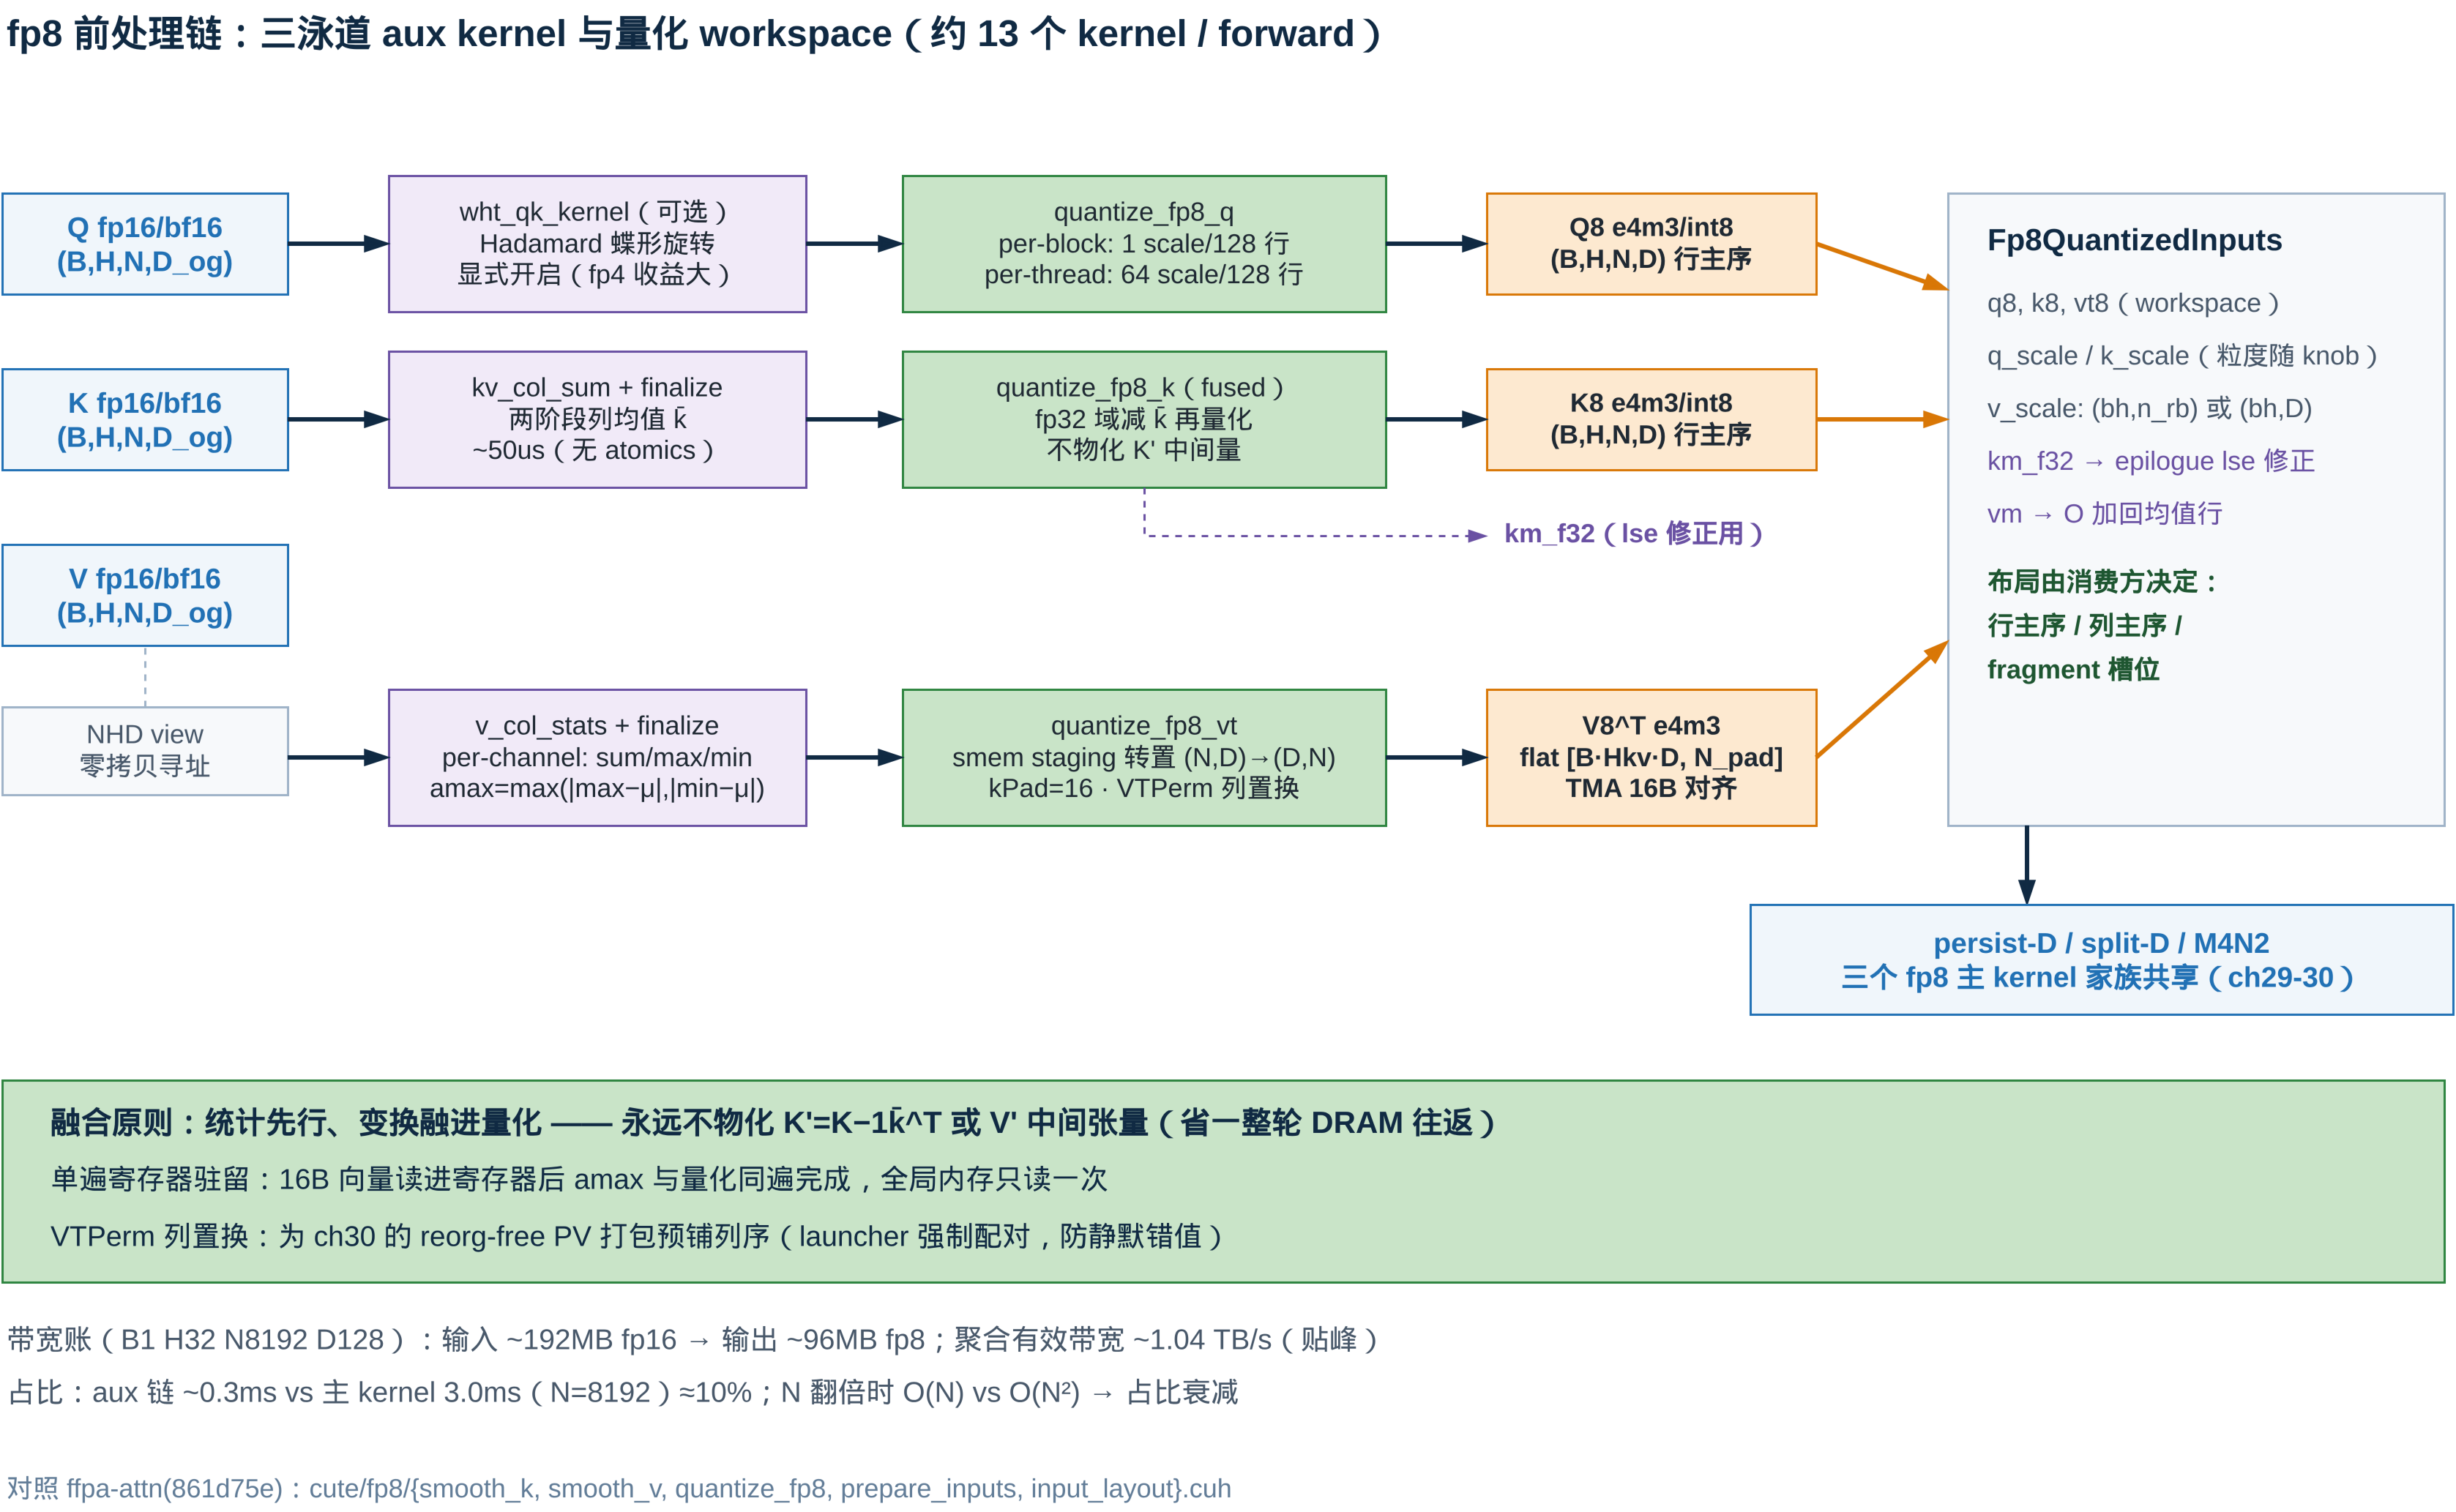
\includegraphics[width=0.98\textwidth]{figures/drawio/fig-28-1-quant-pipeline/fig-28-1-quant-pipeline.png}
  \begin{tikzpicture}[font=\tiny, >=Stealth,
    kin/.style={draw=tkBlue, fill=tkFillBlue, text=tkBlue, align=center, inner sep=2pt,
      font=\bfseries\fontsize{4.2}{4.8}\selectfont},
    kst/.style={draw=tkPurple, fill=tkFillPurple, align=center, inner sep=2pt,
      font=\fontsize{4.2}{4.8}\selectfont},
    kqu/.style={draw=tkGreen, fill=tkFillGreen, align=center, inner sep=2pt,
      font=\fontsize{4.2}{4.8}\selectfont},
    kout/.style={draw=tkOrange, fill=tkFillOrange, text=tkOrange!80!black, align=center,
      inner sep=2pt, font=\bfseries\fontsize{4.2}{4.8}\selectfont},
    pl/.style={anchor=west, align=left, inner sep=1pt,
      font=\fontsize{4.2}{4.8}\selectfont},
  ]
    % 输入列：Q/K/V 的 fp16 张量与 NHD 零拷贝视图
    \node[kin, text width=1.70cm] at (0.90,-0.55) {Q fp16/bf16\\(B,H,N,D\_og)};
    \node[kin, text width=1.70cm] at (0.90,-2.05) {K fp16/bf16\\(B,H,N,D\_og)};
    \node[kin, text width=1.70cm] at (0.90,-3.55) {V fp16/bf16\\(B,H,N,D\_og)};
    \node[draw=gray!60, fill=gray!10, align=center, inner sep=2pt,
      font=\fontsize{4.2}{4.8}\selectfont, text width=1.70cm] at (0.90,-4.45)
      {NHD view\\零拷贝寻址};
    \draw[dashed, gray!70, thin] (0.90,-4.16) -- (0.90,-4.00);
    % Q 泳道：可选旋转 + per-block/per-thread 量化
    \node[kst, text width=2.50cm] at (3.40,-0.55)
      {wht\_qk\_kernel（可选）\\Hadamard 蝶形旋转\\显式开启（fp4 收益大）};
    \node[kqu, text width=2.80cm] at (6.45,-0.55)
      {quantize\_fp8\_q\\per-block: 1 scale/128 行\\per-thread: 64 scale/128 行};
    \node[kout, text width=1.80cm] at (9.15,-0.55) {Q8 e4m3/int8\\(B,H,N,D) 行主序};
    \draw[->, gray!80, semithick] (1.78,-0.55) -- (2.12,-0.55);
    \draw[->, gray!80, semithick] (4.68,-0.55) -- (5.02,-0.55);
    \draw[->, gray!80, semithick] (7.88,-0.55) -- (8.22,-0.55);
    % K 泳道：两阶段列均值 + 融合量化
    \node[kst, text width=2.50cm] at (3.40,-2.05)
      {kv\_col\_sum $+$ finalize\\两阶段列均值 $\bar{k}$\\$\sim$50us（无 atomics）};
    \node[kqu, text width=2.80cm] at (6.45,-2.05)
      {quantize\_fp8\_k（fused）\\fp32 域减 $\bar{k}$ 再量化\\不物化 $K'$ 中间量};
    \node[kout, text width=1.80cm] at (9.15,-2.05) {K8 e4m3/int8\\(B,H,N,D) 行主序};
    \draw[->, gray!80, semithick] (1.78,-2.05) -- (2.12,-2.05);
    \draw[->, gray!80, semithick] (4.68,-2.05) -- (5.02,-2.05);
    \draw[->, gray!80, semithick] (7.88,-2.05) -- (8.22,-2.05);
    \draw[->, dashed, tkPurple, thin] (6.45,-2.48) -- (6.45,-2.78) -- (8.18,-2.78);
    \node[pl, text=tkPurple, font=\bfseries\fontsize{4.2}{4.8}\selectfont] at (8.25,-2.78)
      {km\_f32（lse 修正用）};
    % V 泳道：列统计 + smem 转置量化（列 pad + VTPerm）
    \node[kst, text width=2.50cm] at (3.40,-3.55)
      {v\_col\_stats $+$ finalize\\per-channel: sum/max/min\\
       amax$=\max(|\mathrm{max}-\mu|,\ |\mathrm{min}-\mu|)$};
    \node[kqu, text width=2.80cm] at (6.45,-3.55)
      {quantize\_fp8\_vt\\smem staging 转置 (N,D)$\to$(D,N)\\kPad$=$16 $\cdot$ VTPerm 列置换};
    \node[kout, text width=1.80cm] at (9.15,-3.55)
      {V8$^{\top}$ e4m3\\flat [B$\cdot$Hkv$\cdot$D, N\_pad]\\TMA 16B 对齐};
    \draw[->, gray!80, semithick] (1.78,-3.55) -- (2.12,-3.55);
    \draw[->, gray!80, semithick] (4.68,-3.55) -- (5.02,-3.55);
    \draw[->, gray!80, semithick] (7.88,-3.55) -- (8.22,-3.55);
    % 右侧 workspace 面板
    \node[draw=gray!60, fill=gray!10, align=left, inner sep=3pt,
      font=\fontsize{4.2}{4.8}\selectfont, text width=3.90cm] at (12.60,-2.30)
      {\textbf{Fp8QuantizedInputs}\\
       q8, k8, vt8（workspace）\\
       q\_scale / k\_scale（粒度随 knob）\\
       v\_scale: (bh,n\_rb) 或 (bh,D)\\
       \textcolor{tkPurple}{km\_f32 $\to$ epilogue lse 修正}\\
       \textcolor{tkPurple}{vm $\to$ O 加回均值行}\\
       \textcolor{tkGreen!80!black}{\textbf{布局由消费方决定：}}\\
       \textcolor{tkGreen!80!black}{\textbf{行主序 / 列主序 / fragment 槽位}}};
    \draw[->, tkOrange, semithick] (10.12,-0.55) -- (10.55,-1.10);
    \draw[->, tkOrange, semithick] (10.12,-2.05) -- (10.55,-2.05);
    \draw[->, tkOrange, semithick] (10.12,-3.55) -- (10.55,-3.10);
    % 三个 fp8 主 kernel 家族共享工作区
    \node[kin, text width=4.00cm, font=\bfseries\fontsize{4.4}{5}\selectfont] at (12.60,-5.05)
      {persist-D / split-D / M4N2\\三个 fp8 主 kernel 家族共享（ch29-30）};
    \draw[->, gray!80, semithick] (12.60,-4.35) -- (12.60,-4.72);
    % 融合原则与带宽需求
    \node[draw=tkGreen, fill=tkFillGreen, align=left, inner sep=3pt,
      font=\fontsize{4.4}{5}\selectfont, text width=14.6cm] at (7.55,-6.05)
      {\textbf{融合原则：统计先行、变换融进量化 —— 永远不物化 $K' = K - 1\bar{k}^{\top}$
        或 $V'$ 中间张量（省一整轮 DRAM 往返）}\\
       单遍寄存器驻留：16B 向量读进寄存器后 amax 与量化同遍完成，全局内存只读一次\\
       VTPerm 列置换：为 ch30 的 reorg-free PV 打包预铺列序（launcher 强制匹配，防静默错值）};
    \node[pl, font=\fontsize{4.2}{4.8}\selectfont] at (0.10,-6.90)
      {带宽需求（B1 H32 N8192 D128）：输入 $\sim$192MB fp16 $\to$ 输出 $\sim$96MB fp8；%
       聚合有效带宽 $\sim$1.04 TB/s（接近带宽峰值）};
    \node[pl, font=\fontsize{4.2}{4.8}\selectfont] at (0.10,-7.15)
      {占比：aux 链 $\sim$0.3ms vs 主 kernel 3.0ms（N=8192）$\approx$10\%；%
       N 翻倍时 O(N) vs O(N$^2$) $\to$ 占比衰减};
    \node[pl, text=gray!80!black, font=\fontsize{4.2}{4.8}\selectfont] at (0.10,-7.48)
      {对照 ffpa-attn(861d75e)：cute/fp8/\{smooth\_k, smooth\_v, quantize\_fp8, prepare\_inputs, input\_layout\}.cuh};
  \end{tikzpicture}
  \caption{fp8 前处理链全景：三泳道（Q/K/V）各自的统计 $\to$ 变换 $\to$ 量化
  kernel 与输出 workspace 布局。smoothing 与量化融合在同一 kernel 内（无中间
  落盘）；$V^{\top}$ 的列 pad 兼顾 TMA 16B 对齐与置换写。}
  \label{fig:28-pipeline}
\end{figure}

\begin{figure}[htbp]
  \centering
  % was: 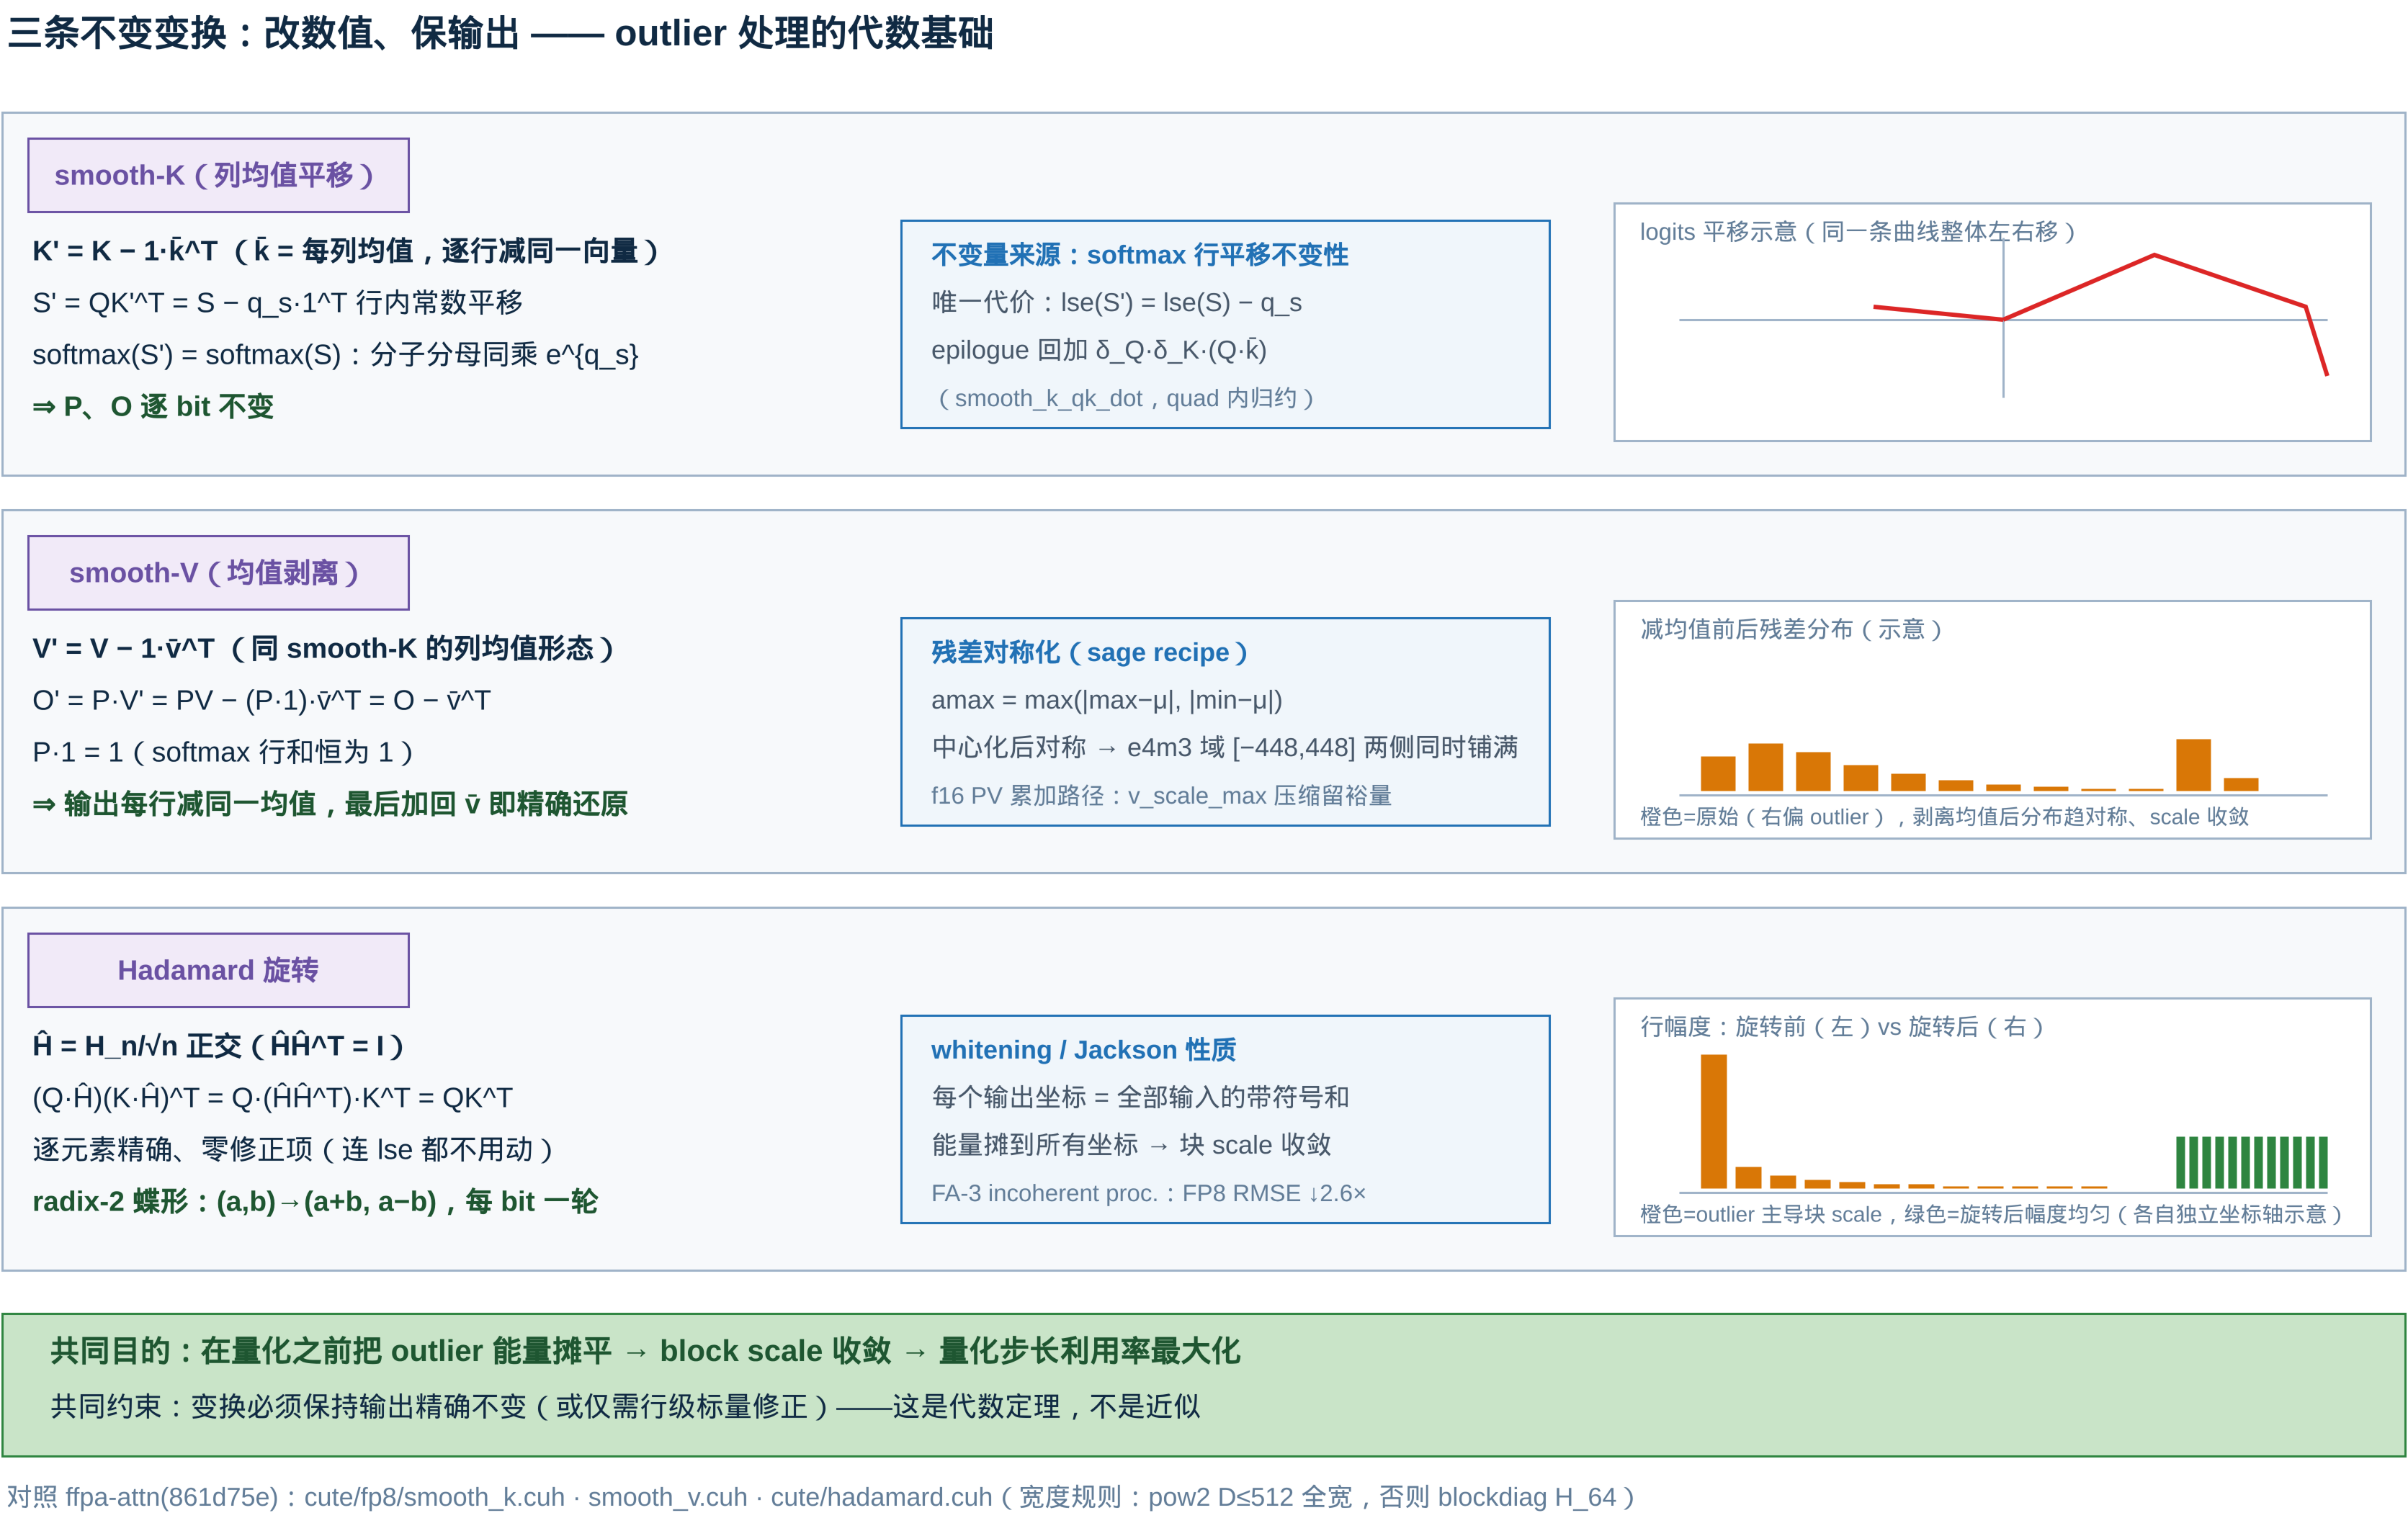
\includegraphics[width=0.98\textwidth]{figures/drawio/fig-28-2-invariants/fig-28-2-invariants.png}
  \begin{tikzpicture}[font=\tiny, >=Stealth,
    lbox/.style={draw=gray!55, fill=gray!8},
    ltag/.style={draw=tkPurple, fill=tkFillPurple, text=tkPurple, align=center, inner sep=2pt,
      font=\bfseries\fontsize{4.6}{5.2}\selectfont},
    tl/.style={anchor=west, align=left, inner sep=1pt,
      font=\fontsize{4.4}{5}\selectfont},
    ib/.style={draw=tkBlue, fill=tkFillBlue, align=left, inner sep=2pt,
      font=\fontsize{4.2}{4.8}\selectfont},
    mi/.style={draw=gray!55, fill=white, inner sep=2pt},
    mn/.style={anchor=west, align=left, inner sep=1pt, font=\fontsize{3.6}{4.2}\selectfont},
  ]
    \foreach \ttop/\tg in {{-0.05/{smooth-K（列均值平移）}},
                            {-2.55/{smooth-V（均值剥离）}},
                            {-5.05/{Hadamard 旋转}}} {
      \draw[lbox] (0.10,\ttop) rectangle (15.40,{\ttop-2.30});
      \node[ltag, text width=2.30cm] at (1.48,{\ttop-0.34}) {\tg};
    }
    % 泳道一：smooth-K —— softmax 行平移不变
    \node[tl, font=\bfseries\fontsize{4.6}{5.2}\selectfont] at (0.35,-0.80)
      {$K' = K - 1\cdot\bar{k}^{\top}$（$\bar{k} =$ 每列均值，逐行减同一向量）};
    \node[tl] at (0.35,-1.13) {$S' = QK'^{\top} = S - q_s\cdot 1^{\top}$\quad 行内常数平移};
    \node[tl] at (0.35,-1.46) {softmax($S'$) $=$ softmax($S$)：分子分母同乘 $e^{q_s}$};
    \node[tl, text=tkGreen!80!black, font=\bfseries\fontsize{4.6}{5.2}\selectfont] at (0.35,-1.82)
      {$\Rightarrow$ P、O 在实数域不变};
    \node[ib, text width=3.85cm] at (8.00,-1.20)
      {\textbf{\textcolor{tkBlue}{不变量来源：softmax 行平移不变性}}\\
       唯一代价：lse($S'$) $=$ lse($S$) $- q_s$\\
       epilogue 回加 scale$\cdot\delta_Q\cdot(\hat Q\cdot\bar{k})$\\
       \textcolor{gray!80!black}{（smooth\_k\_qk\_dot，quad 内归约）}};
    \draw[mi] (10.45,-0.63) rectangle (15.30,-2.20);
    \node[mn, text=gray!85!black] at (10.55,-0.76) {logits 平移示意（同一条曲线整体左右移）};
    \draw[gray!60, thin] (10.75,-1.88) -- (15.05,-1.88);
    \draw[gray!60, thin] (12.90,-1.00) -- (12.90,-2.02);
    \draw[tkRed, semithick] (10.95,-1.90) -- (12.20,-1.20) -- (13.10,-1.78) -- (14.00,-2.00);
    % 泳道二：smooth-V —— 行和为 1 的精确还原
    \node[tl, font=\bfseries\fontsize{4.6}{5.2}\selectfont] at (0.35,-3.30)
      {$V' = V - 1\cdot\bar{v}^{\top}$（同 smooth-K 的列均值形态）};
    \node[tl] at (0.35,-3.63) {$O' = P\cdot V' = PV - (P\cdot 1)\cdot\bar{v}^{\top} = O - \bar{v}^{\top}$};
    \node[tl] at (0.35,-3.96) {$P\cdot 1 = 1$（softmax 行和恒为 1）};
    \node[tl, text=tkGreen!80!black, font=\bfseries\fontsize{4.6}{5.2}\selectfont] at (0.35,-4.32)
      {$\Rightarrow$ 输出每行减同一均值，最后加回 $\bar{v}$ 即精确还原};
    \node[ib, text width=3.85cm] at (8.00,-3.70)
      {\textbf{\textcolor{tkBlue}{残差对称化（sage recipe）}}\\
       amax $=$ max$(|$max$-\mu|, |$min$-\mu|)$\\
       中心化后对称 $\to$ e4m3 域两侧同时铺满\\
       \textcolor{gray!80!black}{f16 PV 累加路径：v\_scale\_max 压缩留裕量}};
    \draw[mi] (10.45,-3.13) rectangle (15.30,-4.70);
    \node[mn, text=gray!85!black] at (10.55,-3.26) {减均值前后残差分布（示意）};
    \draw[gray!60, thin] (10.75,-4.30) -- (15.05,-4.30);
    \foreach \bb/\hh in {0/0.30, 1/0.42, 2/0.34, 3/0.24, 4/0.16, 5/0.10,
                          6/0.06, 7/0.05, 8/0.03, 9/0.03, 10/0.45, 11/0.12} {
      \pgfmathsetmacro{\xb}{10.85+0.16*\bb}
      \fill[tkOrange] (\xb,-4.30) rectangle ({\xb+0.12},{-4.30+\hh});
    }
    \node[mn, text=gray!85!black, text width=4.50cm] at (10.55,-4.52)
      {橙色 $=$ 原始（右偏 outlier）；剥离均值后分布趋对称、scale 收敛};
    % 泳道三：Hadamard 旋转 —— 两端同乘正交阵
    \node[tl, font=\bfseries\fontsize{4.6}{5.2}\selectfont] at (0.35,-5.80)
      {$\hat{H} = H_n/\sqrt{n}$ 正交（$\hat{H}\hat{H}^{\top} = I$）};
    \node[tl] at (0.35,-6.13)
      {$(Q\cdot\hat{H})(K\cdot\hat{H})^{\top} = Q\cdot(\hat{H}\hat{H}^{\top})\cdot K^{\top} = QK^{\top}$};
    \node[tl] at (0.35,-6.46) {逐元素精确、零修正项（连 lse 都不用动）};
    \node[tl, text=tkGreen!80!black, font=\bfseries\fontsize{4.6}{5.2}\selectfont] at (0.35,-6.82)
      {radix-2 蝶形：$(a,b) \to (a{+}b, a{-}b)$，每 bit 一轮};
    \node[ib, text width=3.85cm] at (8.00,-6.20)
      {\textbf{\textcolor{tkBlue}{whitening / Jackson 性质}}\\
       每个输出坐标 $=$ 全部输入的带符号和\\
       能量摊到所有坐标 $\to$ 块 scale 收敛\\
       \textcolor{gray!80!black}{FA-3 incoherent proc.：FP8 RMSE $\downarrow 2.6\times$}};
    \draw[mi] (10.45,-5.63) rectangle (15.30,-7.20);
    \node[mn, text=gray!85!black] at (10.55,-5.76) {行幅度：旋转前（左）vs 旋转后（右）};
    \draw[gray!60, thin] (10.75,-6.80) -- (15.05,-6.80);
    \foreach \bb/\hh in {0/1.00, 1/0.16, 2/0.10, 3/0.07, 4/0.05, 5/0.03,
                          6/0.03, 7/0.02, 8/0.02, 9/0.02, 10/0.02, 11/0.02} {
      \pgfmathsetmacro{\xb}{10.85+0.13*\bb}
      \fill[tkOrange] (\xb,-6.80) rectangle ({\xb+0.10},{-6.80+\hh});
    }
    \foreach \bb in {0,...,11} {
      \pgfmathsetmacro{\xb}{13.25+0.09*\bb}
      \fill[tkGreen] (\xb,-6.80) rectangle ({\xb+0.05},{-6.40});
    }
    \node[mn, text=gray!85!black, text width=4.50cm] at (10.55,-7.02)
      {橙色 $=$ outlier 主导块 scale，绿色 $=$ 旋转后幅度均匀（各自独立坐标轴示意）};
    % 结论
    \node[draw=tkGreen, fill=tkFillGreen, align=left, inner sep=3pt,
      font=\fontsize{4.4}{5}\selectfont, text width=14.6cm] at (7.75,-8.00)
      {\textbf{\textcolor{tkGreen!80!black}{共同目的：在量化之前把 outlier 能量摊平 $\to$
        block scale 收敛 $\to$ 量化步长利用率最大化}}\\
       共同约束：变换必须保持输出精确不变（或仅需行级标量修正）——这是代数定理，不是近似};
    \node[tl, text=gray!80!black] at (0.20,-8.60)
      {对照 ffpa-attn(861d75e)：cute/fp8/smooth\_k.cuh $\cdot$ smooth\_v.cuh $\cdot$
       cute/hadamard.cuh（宽度规则：pow2 $D \le 512$ 全宽，否则 blockdiag $H_{64}$）};
  \end{tikzpicture}
  \caption{三条不变变换的代数结构对比：smooth-K 改 logits 不改概率（lse 回加）、
  smooth-V 改 V 不改 O（行和为 1）、WHT 两端同乘正交阵（收缩逐元素精确）。
  右侧为 outlier 幅度在变换前后的示意（块 scale 收敛）。}
  \label{fig:28-invariants}
\end{figure}

\FloatBarrier

\section{性能分析}

\subsection{带宽需求：为什么 aux 链必须达到带宽峰值}

设 $B\cdot H = 32$、$N = 8192$、$D = 128$、fp16 输入。Q/K/V 总输入字节
$3\times32\times8192\times128\times2\,\mathrm{B} \approx 192\,\mathrm{MB}$；量化
输出（fp8 + scale）约 $96\,\mathrm{MB}$ 出 + $192\,\mathrm{MB}$ 入（若物化 smooth
中间量则为再加一轮 192MB 读 + 192MB 写）。本机（RTX PRO 5000，理论带宽
$\sim$1.34TB/s）实测 aux 链聚合有效带宽约 1.04TB/s，这是\textbf{纯带宽 kernel 的
第一验收指标}。对比 attention 主 kernel（$N=8192$ 时 3.0ms，365T FLOPS）：aux 链
约 0.3ms 量级，占端到端 $\sim$10\%；$N$ 翻倍时主 kernel 时间 $\times4$（$O(N^2)$）
而 aux 链只 $\times2$（$O(N)$），占比随序列长度衰减，所以 aux 优化的优先级
在短序列 / 小 batch 场景最高。

\subsection{每个 kernel 的实测要点}

\begin{itemize}[itemsep=1pt,topsep=2pt]
  \item \textbf{列均值}：库调用 $\sim$85us $\to$ 两阶段自研 $\sim$50us
        （B1 H32 N8192 D128，\texttt{smooth\_k.cuh} 注释实测），省掉 fp32 cast
        的额外往返，同时产出 fp32 副本。
  \item \textbf{per-thread QK}：$\sim$49us（$N=4608$ 量级，D128；数字出自 bench
        留档而非源码注释）。每行两线程
        的网格翻倍是关键（28.4.4~节），冷输入场景 in-flight warp 数直接决定吞吐。
  \item \textbf{fused QKV}：默认路径（\texttt{quantize\_fp8\_qkv\_fused\_kernel}）
        把 Q 量化、K 量化（含 smooth）、V 转置量化合进一个 kernel，三次读
        输入的启动开销与尾部浪费一并省掉。
  \item \textbf{WHT}：一次额外读 + 写（fp16 in-place 语义上），只开 $O(N D\log D)$
        计算，带宽主导，$\sim$数十 us 量级；fp4 块更小（$1\times16$）、outlier
        影响更大，旋转收益最高（bench 默认关，\texttt{--fp4-hadamard} 显式开）。
\end{itemize}

\subsection{粒度的性能代价与 knob 实测}

本章 28.10~节的 A/B（self-attn，D128，$N=8192$，本机 RTX PRO 5000）：基线 fp8
（per-block QK + smooth-K 默认）365T / 1.70$\times$；smooth-V per-channel 369T /
1.72$\times$；强制 per-thread QK 355T / 1.65$\times$。三组差异在 $\pm$2\% 量级
（与跑次间波动同阶）。量化粒度对速度的影响远小于对精度的影响，
knob 化设计建立在这个落差上：精度敏感场景上调粒度，几乎不付性能代价。

\section{实践经验}

\begin{itemize}[itemsep=1pt,topsep=2pt]
  \item \textbf{统计先行、量化融合}：先跑统计 kernel（均值 / 列 amax），再在量化
        kernel 里把变换（减均值）与量化合成一遍读写，不要物化
        $K'$ 或 $V'$ 中间张量，那等于多付一整轮 DRAM 往返。
  \item \textbf{scale 布局跟着消费方走}：per-thread 的 64 槽位表不是随意设定的，它
        精确等于 C-fragment 行对在 128 行块内的索引。任何为 kernel 消费方便
        而做的数据排布决策，都值得在前处理期一次做完。
  \item \textbf{确定性优先于最后一档速度}：列均值用两阶段而非 atomics，牺牲的
        微小速度换来的是数值可复现；精度回归排查（第~\ref{ch:27}~章 27.3.8
        节的 A/B 对比方法）依赖这一点。
  \item \textbf{headdim 泛化在行组映射上}：$D=320/384/448$ 这类非整除组合的坑
        全在 \texttt{kRowsPerIter} 的映射细节（28.4.2~节）；新 headdim 接入要先
        验证这一映射。
  \item \textbf{冷输入的延迟隐藏}：量化 kernel 的输入往往刚被上游 kernel 写出
        （cache 冷），每行两线程这类提高并发度的朴素手段收益显著，胜过任何
        复杂的访存模式。
\end{itemize}

\section{常见坑}

\begin{enumerate}[itemsep=1pt,topsep=2pt]
  \item \textbf{V 的独立布局描述符}：Q/K 与 V 可能来自不同布局（如 Q 是
        BHND、V 是 NHD view）。\texttt{prepare\_fp8\_inputs} 对三者各持一个
        \texttt{Fp8InputLayout}（\texttt{Lq/Lkv/Lv}）；早期版本 K/V 共用描述符，
        NHD 输入时 V 静默读错：数值错但形状合法，只有 allclose 能发现。
  \item \textbf{Hadamard 要求 BHND 物化输入}：
        \texttt{apply\_wht\_qk\_sm120} 假设 contiguous 输入（行 stride 即
        $d_{og}$）；对 NHD view 直接调用会按错误 stride 寻址。launcher 前置了
        物化，但自己复用时必须记得。
  \item \textbf{pad 列的 0/0}：列统计对 pad 列求均值会得 0/0 = NaN；
        \texttt{v\_stats\_finalize\_kernel} 对 pad 列强制 $v\_scale = 1$。所有
        统计与 pad 组合的路径都要过一遍这个检查。
  \item \textbf{kVTPerm 的匹配约束}：置换写只改 $V^{\top}$ 的列序，主 kernel 侧
        的 \texttt{PackC8bitToA8bitPermVT} 必须同开。launcher 做了强制检查，但
        绕过 launcher 直接调 kernel 就没有保护，错配是静默错值。
  \item \textbf{e4m3 的 448 与 f16 累加域}：$v_{scale\_max}$ 在 f16 PV 累加路径
        要压缩（28.3.2~节）；忘了压缩时 f16 域的多块累加会在长序列溢出，
        表现为短序列正确、长序列偶发 inf。
\end{enumerate}

\section{面试要点速查}

\begin{enumerate}[itemsep=1pt,topsep=2pt]
  \item smooth-K 为什么不改注意力输出？lse 要怎么修？
        （行平移不变性；$\mathrm{lse}$ 回加 $\delta_Q\delta_K\, q_{s,m}$，
        式~\ref{eq:28-smk-shift}--\ref{eq:28-smk-invariant}。）
  \item smooth-V 的均值剥离凭什么精确可逆？（$P\mathbf{1}=\mathbf{1}$，
        式~\ref{eq:28-smv-invariant}；输出加回 $\bar v$，无 lse 项。）
  \item Hadamard 旋转保持 $QK^{\top}$ 精确不变靠什么？为什么它能降量化误差？
        （正交消去式~\ref{eq:28-wht-orth}；whitening / Jackson 性质分散 outlier
        能量，块 scale 收敛。）
  \item per-thread 量化粒度为什么是 64 scale / 128 行？怎么来的？
        （C-fragment 行对 $\{r,r+8\}$ 在 128 行块内的 $8\times8$ 索引；
        零 shuffle 反量化，28.3.4~节。）
  \item $V^{\top}$ 量化为什么要 smem staging？pad 16 列起什么作用？
        （读行主序写列主序，两侧都要合并；TMA 16B 对齐 + bank 错开。）
  \item NHD 布局怎么零拷贝进量化 kernel？（布局描述符 + 平面基址式
        \ref{eq:28-plane-base}；输出统一 BHND。）
  \item 两阶段列均值相比 atomics 方案牺牲了什么、换来了什么？
        （多一次 partial 读写，换确定性与去掉 zero-init。）
\end{enumerate}

\section{最小测试与动手实验}

本章无独立 kernel 测试（Part VI 以 \texttt{ffpa\_attn.bench} CLI 为验收），全部
数据在 RTX PRO 5000（sm\_120）实测，命令在仓库根目录执行：

\begin{lstlisting}[style=console]
# 环境（Card 7，小 headdim 放行）
$ conda activate cdit
$ export CUDA_VISIBLE_DEVICES=7 FFPA_CUDA_ALLOW_SMALL_D=1

# [A] 基线：默认 fp8（per-block QK + smooth-K）
$ python -m ffpa_attn.bench --fwd-backend cuda --cuda-impl fp8 \
    --tasks self-attn --D 128 --no-bwd --show-allclose
# self-attn fp16  8192/8192  3.01ms  365T  1.70x  allclose OK

# [B] 强制 smooth-K（等价别名 --cuda-impl fp8_smk）
$ python -m ffpa_attn.bench --fwd-backend cuda --cuda-impl fp8 \
    --tasks self-attn --D 128 --no-bwd --show-allclose --fp8-smooth-k
# 3.02ms  365T  1.70x  allclose OK

# [C] smooth-V：per-channel V + 维度均值剥离
$ python -m ffpa_attn.bench --fwd-backend cuda --cuda-impl fp8_smv \
    --tasks self-attn --D 128 --no-bwd --show-allclose
# 2.98ms  369T  1.72x  allclose OK

# [D] per-thread QK 粒度
$ python -m ffpa_attn.bench --fwd-backend cuda --cuda-impl fp8 \
    --tasks self-attn --D 128 --no-bwd --show-allclose \
    --fp8-q-quant-method per-thread --fp8-k-quant-method per-thread
# 3.10ms  355T  1.65x  allclose OK
\end{lstlisting}

\textbf{实验 1（粒度谱系）}：固定 D128 self-attn，扫
\texttt{--fp8-q-quant-method} 三档（per-block / per-channel / per-thread），
记录每档速度与 \texttt{--show-allclose} 的最大误差档位；验证粒度升一档、
精度相应提升、速度几乎不变。
\textbf{实验 2（smooth 开关）}：对比 A/B/C 三组的 allclose 分布（不止看布尔值，
把 bench 的误差打印调出来），观察 smooth-K 对 QK 误差、smooth-V 对 PV 误差的
分别贡献。
\textbf{实验 3（aux 占比）}：把 \texttt{--tasks} 换成 \texttt{cross-attn} 并把
$N$ 从 1024 扫到 8192（\texttt{--seqlens}），观察 aux 链占比随 $N$ 的衰减，
验证 28.6.1~节的 $O(N)$ vs $O(N^2)$ 论断。
\textbf{实验 4（WHT）}：fp4 路径（\texttt{--cuda-impl fp4}）开关
\texttt{--fp4-hadamard}，对比精度：WHT 对 16 元素小块的 outlier 抑制在小 headdim
上最显著（第~\ref{ch:31}~章将回到这个实验）。

\section*{延伸阅读}
\begin{itemize}[itemsep=0pt,topsep=2pt]
  \item SageAttention（arXiv:2410.02367）\S3：smooth-K/V 的原始动机与精度消融。
  \item FlashAttention-3（arXiv:2407.08608）\S3.3：incoherent processing，
        Hadamard 旋转与分块量化联合降 FP8 RMSE $2.6\times$ 的出处。
  \item QuaRot（arXiv:2404.00456）：旋转扩散 outlier 到全坐标的端到端量化框架
        （比本章的单层 attention 旋转更一般化）。
  \item SageAttention2（arXiv:2411.10958）：per-thread 粒度与 fp8 PV 的工程组合。
  \item ffpa-attn \texttt{cute/fp8/quantize\_fp8.cuh} 头注释：int8 对称量化
        recipe 的代码级规范（SageAttention \texttt{qattn} 的实现对照）。
\end{itemize}

% ch29-fp8-persist-d.tex — FP8(二)：persist-D 主 kernel 与 scale 折叠代数（RFC-K3）★
% 源码：ffpa-attn(861d75e) cute/fp8/sm_120/persist_d.cuh(1036L) + fp8_pscale.cuh(304L)
%       + softmax.cuh(344L) + reg2reg_8b.cuh(163L) + attn_traits.cuh(313L)
\chapter{FP8（二）：persist-D 主 Kernel 与 Scale 折叠代数}\label{ch:29}

\section{本章导读}

第~\ref{ch:28}~章把 fp16 输入变成了量化 workspace（$Q_8,K_8,V_8^{\top}$ 与
scale 张量）；本章进入主 kernel，即文件 \texttt{sm\_120/persist\_d.cuh} 里的
\texttt{persist\_d\_ws\_fwd\allowbreak{}\_cute\_fp8\allowbreak{}\_sm120}（sm\_120 warp-specialized
persist-D，全文件 1036 行）。它是 ffpa-attn 全仓库实现最密集的单个文件，
也是 Part VI 的核心章：第~\ref{ch:30}~章的 split-D / M4N2 与
第~\ref{ch:31}--\ref{ch:32}~章的 fp4 家族都建立在它引入的机制之上。

本章的主线只有一条：让所有量化 scale 因子要么在未舍入代数中精确消去、
要么折进本来就要做的操作。理想目标是在实数代数模型下除 round() 外没有额外
代数误差源；浮点执行仍有乘加、exp2 与累加舍入。围绕这条主线展开五组机制：
\begin{enumerate}[itemsep=0pt,topsep=2pt]
  \item \textbf{QK scale 折进 exp2 系数}：$\delta_Q\delta_K$ 与 softmax scale
        融成单个 fp32 系数；per-block 下可在 tile max 归约后一次乘入（29.3.1~节）；
  \item \textbf{$v_s$ 在未舍入 scale 代数中精确消去}：P 发射
        $\tilde P = P\cdot v_s\cdot448$，gmem 中的 $\hat V = V/v_s$ 原样复用，
        $v_s$ 从 PV 的 scale 代数中消失（29.3.2~节的三步协议）；
  \item \textbf{归约轴置换不变性}：P fragment 打包零 SHFL，代价转移到
        $V^{\top}$ 的列置换（29.3.5~节，第~\ref{ch:28}~章预告内容的展开）；
  \item \textbf{WS persist-D 结构}：128 producer + 256 consumer、
        \texttt{setmaxnreg} 32/232、Q 的 s2r 常驻与 K 槽位 0（Q 区）复用给
        最后一个 K stage（29.4.2--29.4.3~节）；
  \item \textbf{发射域规则}：fixed 发射上界 $\mathrm{amax}(V)$ vs per-channel
        满量程发射 448、满量程发射与 lazy rescale 互斥、f16 PV 累加域整 tile
        预算 $kBc\cdot P_r\cdot V_r\le65504$（29.3.3--29.3.4~节）。
\end{enumerate}

\textbf{前置章节}：第~\ref{ch:17}~章（TMA+WS 双流水）、第~\ref{ch:22}~章
（TiledMMA 与 fragment）、第~\ref{ch:23}~章（swizzle）、第~\ref{ch:27}~章
（量化数学，必须）、第~\ref{ch:28}~章（前处理链，必须）。
\textbf{源码区间}：\texttt{sm\_120/persist\_d.cuh} 全文、
\texttt{fp8\_pscale.cuh} L72--300、\texttt{reg2reg\_8b.cuh} 全文、
\texttt{attn\_traits.cuh} L1--110、\texttt{softmax.cuh} L44--63；行号以
附录~\ref{app:D}~的 commit permalink 为准。
\textbf{验证方式}：\texttt{ffpa\_attn.bench} CLI，D=64/128 全绿；
D=192 本机实测发现正确性 bug，完整定位过程记在 29.7.1~节。

\section{问题与动机}

\subsection{主 kernel 的输入约定}

从第~\ref{ch:28}~章的 \texttt{Fp8QuantizedInputs} 出发，主 kernel 消费：
$Q_8\in$ e4m3/int8 $(N,kD)$ 行主序、$K_8$ 同构、$V_8^{\top}\in$ e4m3
逻辑 $(kD,N_{pad})$ 行主序，$N$ 维连续（含 \texttt{VTPerm} 置换与 16 列 TMA pad）、三组
scale（布局随粒度）、smooth-K 的 fp32 均值（lse 修正用）。主 kernel 的任务
是在 warp-specialized 流水线里完成 $O = \mathrm{softmax}(QK^{\top})V$ 的
分块在线计算，同时把 scale 的代数消去融进流水线的每个阶段，而不是
算完后统一反量化。

\subsection{为什么 scale 消去是核心矛盾}

低精度 MMA 对 e4m3/int8 等低位宽数值做乘累加（e4m3 仍是浮点语义，累加器可为 f32；int8 路径才是整数累加），而 attention 的
数学在实数域。朴素的每个操作数先乘回 scale 方案意味着每 tile 数千次
额外 FMUL 与中间张量往返，fp8 MMA 吞吐翻倍的收益会被反量化开销抵消大半。
第~\ref{ch:27}~章 27.3.4~节给过 scale 流向总览；本章把它们逐一落到代码：
每个 scale 在哪个寄存器、哪条指令上被消去，以及哪些组合会互相冲突
（如 lazy rescale 与满量程 P）。

\subsection{persist-D 的适用域与家族分工}

persist-D 服务 $D\in\{32,64,\dots,224\}$（32 的倍数）：Q tile 整块常驻、
K/V 沿序列方向分块流过。$D$ 更大时 Q tile 无法整块驻留寄存器，交给
split-D（M8N1，$224<D<768$）与 M4N2（$D\ge768$）：见第~\ref{ch:30}~章。
本机（RTX PRO 5000）编译的 headdim 集为 $\{64,128,192,256,320,512\}$，
本章 bench 覆盖 persist-D 域内的 64/128/192。

\section{数学原理}

\subsection{QK 反量化折进 log2 域 softmax}\label{sec:29-qk-fold}

$\hat S=\hat Q\hat K^{\top}$ 是量化域乘加：int8 路径为整数累加，e4m3 路径为浮点乘加以 f32 累加。
per-block 下真实 $S=\hat S\cdot\delta_Q\delta_K$；per-thread 下应逐元素写
$S_{ij}=\hat S_{ij}q_{s,i}k_{s,j}$，$q_s,k_s$ 分别随行与列组变化。softmax 需要的是
$\exp(\mathrm{scale}\cdot S)$。先把 per-block 的 $\delta_Q\delta_K$ 与 softmax scale、
$\log_2 e$ 融成单个 fp32 系数：
\begin{equation}
  \exp\big(\mathrm{scale}\cdot\delta_Q\delta_K\cdot\hat S\big)
  =\exp_2\!\big(\underbrace{\mathrm{scale}\cdot\delta_Q\delta_K\cdot\log_2 e}_{\text{单个
  fp32 系数}}\cdot\hat S\big),
  \label{eq:29-sdequant}
\end{equation}
per-block 下该系数对行内各列一致，可在 tile max 归约之后一次乘入
（\texttt{kMaxScaleAfter}：29.4.3~节），每元素省一次 FMUL。per-thread 则先逐元素乘
$q_s k_s$；即使 \texttt{kMaxScaleAfter} 为真，后移的也只含剩余 softmax scale。

int8 变体走 \texttt{s8xs8$\to$s32} MMA，s32 累加器原位 cast 到 f32 寄存器后同样处理。
int8 均匀步长使 $S$ 的绝对误差有均匀上界，在近 max（大 $|S|$）的 softmax
主导区相对误差更小，且 s32 累加精确（无 f8f8f32 累加舍入），这是 int8 QK 在
大 $N$ 下更优的根源。

\subsection{P 量化三步协议与 $v_s$ 的 scale 代数消去}\label{sec:29-pscale}

$P$ 只能在线量化（27.2.2~节 P 无法离线）。\texttt{fp8\_pscale.cuh} 的
三步协议把 $v_s$（V 的量化 scale）从 PV 的未舍入 scale 代数中精确消去。
\begin{equation}
  \hat P=\mathrm{round}\!\Big(\frac{P\cdot v_s}{p_{scale}}\Big),\qquad
  \frac{P\,v_s}{p_{scale}}\cdot\frac{V}{v_s}=\frac{PV}{p_{scale}},\qquad
  \mathrm{MMA}=\hat P\,\hat V\approx\frac{PV}{p_{scale}},\qquad
  O\mathrel{+}=\mathrm{MMA}\cdot p_{scale} \approx PV .
  \label{eq:29-threestep}
\end{equation}
中间的 scale 等式是实数代数恒等式；$\hat P,\hat V$ 的量化舍入仍保留。
$v_s$ 消去的直接推论：\textbf{gmem 中预量化的 $\hat V$ 原样复用}，主 kernel
从不需要 $V$ 的 fp16 原件。

$v_s$ 被折进 P 侧的发射域
$\tilde P = P\cdot v_s\cdot448$。fixed 模式下 $p_{scale}\equiv1/448$（编译期
常数），epilogue 用 $(1/448)/\mathrm{rowsum}$ 一步完成反量化与
归一化。

fixed vs per-row 的取舍：
\begin{itemize}[itemsep=1pt,topsep=2pt]
  \item \textbf{fixed（默认）}：$\tilde P = P\cdot v_s\cdot448$，per-block V 时
        $v_s=\mathrm{amax}(V)/448$，发射上界是 $\mathrm{amax}(V)$ 本身而非 448
        （留有 $448/\mathrm{amax}(V)$ 的 headroom，见 29.3.3）；$o\_acc$ 全程单一
        $448\times$ 域，rescale 可折进吸收 FFMA
        （29.4.3~节）。代价：$\max(P)\ll1$ 的平坦行（causal 顶部）只用发射域的
        一小部分。
  \item \textbf{per-row}（\texttt{FFPA\_FP8\_PQUANT\_PER\_ROW=1}）：
        $p_{scale}[row]=\mathrm{rowmax}(P)/448$ 按行自适应归一，每行铺满发射域，
        精度最优；代价是跨 lane rowmax 归约、64-float $o\_tile$ 暂存（寄存器
        压力），且\textbf{与 lazy rescale 互斥}（29.3.3，满量程发射零 headroom）。
\end{itemize}

\subsection{lazy rescale 的溢出约束与 fp8 的关闭}\label{sec:29-lazy}

FA-4 式 lazy rescale（27.3.6~节）允许 stale max 落后 $T$ 位才补 rescale，
期间发射的 $P$ 按 stale max 膨胀 $2^T$。fixed + per-block V 的发射上界是
$\mathrm{amax}(V)$（29.3.2），lazy 的安全条件是膨胀后不越 e4m3 上限：
\begin{equation}
  2^T\cdot\mathrm{amax}(V)\le448
  \;\Longrightarrow\;
  T=4\Rightarrow \mathrm{amax}(V)\le28 .
\end{equation}

但 ffpa 的 traits 把 fp8 的 \texttt{kLazyRescale} 直接置 \texttt{false}
（\texttt{attn\_traits.cuh} L31--37）。注释给的理由是：跳过 rescale 会让发射 P
以最高 $2^T$ 膨胀，而 per-channel V 路径（balanced narrowing）的发射
$P\cdot448$ 已铺满量程、零 headroom，膨胀必然触发 satfinite 钳位、破坏 PV
结果。f16 inst\_buf 路径则把 rescale 融进吸收 FFMA 后\textbf{立即 rescale 几乎零
开销}，lazy 的动机（省 rescale pass）本身就消失了。\textbf{满量程发射与延迟 rescale
不可兼得}，这是发射域规则的第一条。

\subsection{f16 PV 累加器的域约束}\label{sec:29-f16acc}

SA2++ 的 \texttt{mma.f16.f8.f8.f16} 让 PV 累加器走 f16 域（把 $o\_acc$
从 tensor-core 反馈链上移出来，避开 f8f8f32 累加器 22-bit 尾数损失）。
SA2++ 论文的核算口径是单条 MMA 指令：$m16n8k32$ 的 K 深度 32，逐元素
乘积需满足 $P_r\times V_r\le65504/32=2047$，两侧同收（$P_r=224,V_r=4.5$）。
ffpa 的累加结构不同：PV 经 \texttt{gemm\_rs} 跨整个 $kBc$ 块累进同一组 f16
\texttt{inst\_buf} 寄存器、之后才一次性 FFMA 吸收进 f32 $o\_acc$
（29.4.3~节 Phase 4），有效界是整 tile 累加：
\begin{equation}
  kBc\cdot P_r\cdot V_r \le 65504 .
  \label{eq:29-f16tile}
\end{equation}

ffpa 的分配\textbf{只收紧 V 侧}：per-channel V + f16 acc 时发射
$\hat V\in[-2.25,2.25]$（即 28.3.2~节的 $v_{scale\_max}=2.25$）。P 侧在
$kBc\le64$ 时保持 448 满量程（$64\times448\times2.25=64512\le65504$$\checkmark$），
$kBc=128$ 时预算超限，kernel 侧的编译期自动收窄
（\texttt{persist\_d.cuh} L723--732）把 P 域收到 224
（$128\times224\times2.25=64512$$\checkmark$）。f32 acc 时无 f16 溢出界，V 侧取满
448、P 侧恒 448 无约束。

\begin{figure}[H]
\centering
\begin{tikzpicture}[font=\scriptsize]
  \definecolor{budgetok}{RGB}{40,110,60}
  \definecolor{budgetbad}{RGB}{170,35,35}
  \def\yup{2.62}
  \draw[->] (0,0) -- (4.62,0);
  \draw[->] (0,0) -- (0,6.68);
  \foreach \yv/\yl in {0/0,1.6/40,3.2/80,4.8/120,6.4/160}{
    \draw (-0.07,\yv) -- (0.07,\yv);
    \node[left, font=\tiny, inner sep=1pt] at (-0.10,\yv) {\yl};
  }
  \node[anchor=south west, font=\tiny] at (0.03,6.44) {$\times10^3$};
  \foreach \xl/\xr in {0.12/0.50,1.45/1.75,2.50/3.00,3.75/4.34}{
    \draw[budgetbad, thick, densely dashed] (\xl,\yup) -- (\xr,\yup);
  }
  \node[budgetbad, anchor=west, font=\tiny, align=left] at (4.68,2.62)
    {f16 溢出上限\\65504};
  \fill[budgetok!16] (0.50,0) rectangle (1.45,2.58);
  \draw[thick] (0.50,0) rectangle (1.45,2.58);
  \fill[budgetbad!16] (1.75,0) rectangle (2.70,5.16);
  \draw[budgetbad, thick] (1.75,0) rectangle (2.70,5.16);
  \fill[budgetok!16] (3.00,0) rectangle (3.95,2.58);
  \draw[thick] (3.00,0) rectangle (3.95,2.58);
  \node[font=\tiny] at (0.975,2.08) {64512};
  \node[font=\tiny] at (2.225,4.62) {129024};
  \node[font=\tiny] at (3.475,2.08) {64512};
  \node[budgetok, font=\scriptsize] at (0.975,3.02) {$\checkmark$};
  \node[budgetbad, font=\scriptsize] at (2.225,5.62) {$\times$};
  \node[budgetok, font=\scriptsize] at (3.475,3.02) {$\checkmark$};
  \node[below, font=\tiny, align=center, inner sep=1pt] at (0.975,-0.10)
    {$k_{Bc}{=}64$\\P 域 448};
  \node[below, font=\tiny, align=center, inner sep=1pt] at (2.225,-0.10)
    {$k_{Bc}{=}128$\\P 域 448};
  \node[below, font=\tiny, align=center, inner sep=1pt] at (3.475,-0.10)
    {$k_{Bc}{=}128$\\P 域 224};
  \begin{scope}[xshift=7.30cm]
    \draw[->] (0,0) -- (2.85,0);
    \draw[->] (0,0) -- (0,3.42);
    \foreach \yv/\yl in {0/0,0.68/500,1.37/1000,2.05/1500,2.73/2000}{
      \draw (-0.07,\yv) -- (0.07,\yv);
      \node[left, font=\tiny, inner sep=1pt] at (-0.10,\yv) {\yl};
    }
    \fill[budgetok!16] (0.45,0) rectangle (1.25,1.37);
    \draw[thick] (0.45,0) rectangle (1.25,1.37);
    \node[font=\tiny] at (0.85,0.56) {1008};
    \node[budgetok, font=\scriptsize] at (0.85,1.62) {$\checkmark$};
    \draw[budgetbad, thick, densely dashed] (0.08,2.79) -- (2.60,2.79);
    \node[budgetbad, anchor=south west, font=\tiny] at (0.12,2.84) {2047};
    \node[below, font=\tiny, align=center, inner sep=1pt] at (0.85,-0.10)
      {$P_r{\times}V_r$\\$224{\times}4.5$};
    \node[anchor=south, font=\tiny, align=center] at (1.45,3.50)
      {SA2++ 单指令口径\\($K$ 深度 32)};
  \end{scope}
  \node[anchor=north west, align=left, text width=10.6cm, font=\tiny] at (-0.55,-1.30)
    {ffpa 的界是\textbf{整 tile 累加}：PV 经 \texttt{gemm\_rs} 跨整个 $kBc$ 块累进同一组
     f16 \texttt{inst\_buf}（之后才 FFMA 吸收进 f32 $o\_acc$），条件为
     $kBc\cdot P_r\cdot V_r\le65504$——$kBc{=}64$ 等效 $P_r{\times}V_r\le1023$，
     $448\times2.25=1008$ 恰好在上限内；$kBc{=}128$ 装不下，编译期把 P 域收窄到 224
     （\texttt{persist\_d.cuh} L723--732）。SA2++ 的单指令界（$65504/32=2047$，$K$ 深度更小）
     更松。f32 acc 无 f16 溢出界：V 侧取满 448、P 侧恒 448。};
\end{tikzpicture}
\caption{f16 PV 累加器的整 tile 域预算（式~\ref{eq:29-f16tile}）。条形为
$kBc\times P_r\times V_r$：$k_{Bc}{=}64$ 与\textbf{$k_{Bc}{=}128$ + P 域自动收窄到 224}
都恰为 64512，接近 65504 上限；$k_{Bc}{=}128$ 且 P 仍 448 则 129024 约 2 倍超限。
右：SA2++ 按单条 MMA（$K{=}32$）核算的界 2047 更松（$P_r{=}224,V_r{=}4.5$ 双侧收窄）。
f32 acc 路径无此约束。}
\label{fig:29-f16-budget}
\end{figure}

\subsection{归约轴置换不变性与 reorg-free 打包}\label{sec:29-perm}

softmax 产出的 $P$ fragment（QK MMA 的 C 布局）与 PV MMA 的 A 操作数布局
不一致（29.4.4~节有完整布局推导）。传统解法是按每 128 列 tile、每线程
16 SHFL + 32 PRMT 的跨 lane 重排。

数学出路是归约轴双射不变性。
\begin{equation}
  \sum_k P[m,k]V[k,n]=\sum_k P[m,\pi(k)]\,V[\pi(k),n]
  \qquad(\pi\ \text{任意双射}) .
  \label{eq:29-perm-inv}
\end{equation}
既然 $\pi$ 任意，就让 P 留在本 lane、按本 lane 已持有的字节就地打包：
每个 $K{=}32$ 组 4 条 lane 无关 PRMT，128 列共 16 条，零 SHFL。
A 操作数携带一个置换的 k 索引 $\pi$。V 侧
在量化期按 $\pi^{-1}$ 预置换列序（\texttt{VTPermInv32}，式~\ref{eq:28-vtperm}），
两侧槽位对应同一真实 kv 位置即可。

row-sum MMA（B 为全 1）在双射下也
精确。这条原则落到实现上就是一次等价替换：kernel 内的 16 次跨 lane shuffle
换成了量化期的列置换。

\section{设计与实现}

\subsection{traits：把配置变成类型}

\begin{lstlisting}[
  caption={persist-D fp8 traits 的关键常量（\texttt{attn\_traits.cuh} L9--42，节选）},
  label={lst:29-traits}]
// Persist-D FP8 traits: fp8 e4m3 Q/K/V via SM89 m16n8k32 mma.sync.
// V is pre-transposed by the quantize pre-kernel and stored (D x N), so the PV
// B-operand loads with the same non-transposed LDSM_N atom as Q/K; there is no
// SmemCopyAtomTransposed for fp8. TiledMma K-tile is 32 (atom K), not 16.
// kQKInt8: Q/K become symmetric int8 and QK runs SM80 m16n8k32 s8xs8->s32
// (A/B operand layouts identical to the fp8 atom; acc is s32, cast in-kernel);
// V/PV stay fp8 e4m3.
template <int kHeadDim_, typename ElementO_, int kBr_ = 128, int kBc_ = 64,
          int kStagesK_ = 2, int kStagesV_ = 2, bool kQKInt8_ = false>
struct FFPAAttnCuTePersistDFP8Traits {
  // Lazy (FA-4 deferred) rescale is OFF for fp8 precision: skipping a rescale
  // leaves the running max stale, so emitted P is inflated by up to
  // 2^FFPA_RESCALE_THRESHOLD_FP8 against that stale max; with P spanning the
  // e4m3 range (balanced narrowing) the inflation hits satfinite and corrupts
  // the PV result.
  static constexpr bool kLazyRescale = false;
  static constexpr int kSmemElems =
      kBr * kHeadDim + kStagesK * kBc * kHeadDim + kStagesV * kBc * kHeadDim;
\end{lstlisting}

traits 里有四处类型决策。$V^{\top}$ 的 B 操作数用与 Q/K 相同的非转置
LDSM\_N atom，因为 V 已在 gmem 里转置好，kernel 里没有转置视角。
TiledMma 的 K-tile 是 32，对应的 fp8 atom 本身就是 $K{=}32$（m16n8k32），
不是 fp16 的 k16 atom；fp16 家族的 K-tile 是 16。swizzle atom 按行字节选（L45--50）：Q/K 行 $D$ 字节、
$V^{\top}$ 行 $kBc$ 字节，各自落 SW128/SW64/SW32：同一张 smem 图、两类
行宽分别选择各自的 swizzle atom。

kBc 随 D 切换：launcher 对 $D\le128$ 实例化 $kBc{=}128$、
$D>128$ 用 64（smem 预算）。

\subsection{WS 骨架与 smem 复用}

128 线程 producer（TMA 装载）+ 256 线程 consumer（全部计算），
\texttt{\_\_launch\_bounds\_\_(384,1)}；寄存器经 \texttt{setmaxnreg}
重分配：producer 释放到 32，consumer 得到 232。fp8 路径的 consumer
无条件使用 232（fp16 版在 D=128 时只需 170）：P 量化 + row-sum + rescale
状态推高了寄存器压力，注释记录\textbf{静态 170 上限会 spill 约 60 个寄存器}。

\begin{lstlisting}[
  caption={Q smem 复用与槽位轮转（\texttt{persist\_d.cuh} L193--215，节选）},
  label={lst:29-smem}]
  // SMEM: [Q | K stages | V stages], 1B per elem (int8 or e4m3). With
  // kPersistQs2r the Q tile is read into regs once before the kv loop, so
  // its 16KB area (slot 0 of the K region) is reused by the LAST K stage
  // and the Q bytes drop out of the allocation: smem = (kStagesK +
  // kStagesV) K/V tiles, e.g. stages 2 -> 64KB (vs 80KB keeping a dead Q
  // tile). The saving buys L1, not occupancy: smem/L1 share one pool per SM
  // (~4-5us per 16KB), and residency stays register-limited (1 CTA/SM)
  // either way.
  // kPersistQs2r slot rotation: logical stage s -> physical slot (s+1) %
  // kStagesK, so the Q area (slot 0) hosts the LAST stage. That stage's
  // first TMA issue happens in steady state (k_tile == kStagesK-1) and its
  // first consume is tile kStagesK-1, hiding the q_consumed wait behind a
  // full tile of compute; the prologue stages (slots 1..) never touch the
  // Q area and issue with no Q dependency at all.
  constexpr auto kKSlot = [](int s) {
    return kPersistQs2r ? (s + 1) % kStagesK : s;
  };
\end{lstlisting}

两层设计叠加。Q 的 s2r 常驻（\texttt{kPersistQs2r} 默认 true）：
Q 在 kv 循环前一次性读进寄存器，之后 QK 步骤全是 gemm\_rs（K-only smem 读）：
D=128 实测 $-8\mu s$、零 spill；Q 的 smem 区（slot 0）随即空闲。
槽位轮转让复用区承接最后一个 K stage 而非第一个：它的首次 TMA
发射与首次消费都发生在稳态（隔着一整 tile 计算），\texttt{q\_consumed} 的
等待被完全隐藏。省下的 16KB smem 换来的是 L1 容量而非 occupancy：smem/L1
共池，实测每 16KB $\approx$ 4--5$\mu s$，而 CTA 驻留本就被寄存器限制在
1/SM。

producer 的装载序还有两处细节：\texttt{V prologue 先于 K}（V0 只在
QK0+softmax 之后才被消费，提前发射是安全的）；consumer 在等 Q 之前先
\texttt{arrive} 全部初始 \texttt{k\_empty}/\texttt{v\_empty}（这些 arrive
不依赖 Q 数据，提前放行让 K(0)/V(0) 的 TMA 与 Q 的 TMA 在传输中重叠）。

\subsection{主循环：五个 Phase 的数据通路}

consumer 的 kv 循环（\texttt{\#pragma unroll 1}，逐 tile）：

\textbf{Phase 1 -- QK GEMM}（L583--601）：等 \texttt{k\_full}、fence、
\texttt{gemm\_rs(tCrS, tCrQ, tCrK, ...)}：Q 在寄存器、K 从 smem 流入。
int8 变体把 s32 累加器\textbf{原位} cast 成 f32（复用同一组 4B 寄存器），
零额外寄存器。scale 粒度在读取处分叉：per-block 的 $k_s$ 是每 tile 一个
标量；per-thread 的 $k_s$ 按
\texttt{(wg\_tid\%32)\%4} 列组查表（4 scale/块，SM80\_16x8 C-fragment 的
lane$\to$列对映射），$q_s$ 按行查 \texttt{qs\_arr[row]}
（$\{r,r{+}8\}$ 行对共享）。

\textbf{Phase 2 -- log2 域 softmax}（L649--790）：mask（causal
tail-aligned 的 \texttt{mask\_start\_tile}/\texttt{Tc\_eff} 两级剪枝，
尾 tile 内逐元素 $-\infty$）；随后
\texttt{online\_softmax\_fp8\_fixed} 以 $\log_2(p\_quant\_scale)$ 为
exp2 偏移，softmax \textbf{直接发射} $\tilde P = P\cdot v_s\cdot448$，即
式~\ref{eq:29-threestep} 的 (1) 步折进 softmax 本身。\texttt{kMaxScaleAfter}
（int8+f16acc 配置）的效果按 QK 粒度分叉：per-block 的 tile max 直接归约原始
scores，跨 lane 归约后一次乘 $\delta_Q\delta_K\cdot$scale；per-thread 则在进入
softmax 前逐元素乘回 $q_sk_s$，tile max 已含这层反量化，后移的只是剩余
softmax scale。两种路径都把 max 的乘入放在跨 lane 归约后。

\textbf{Phase 3 -- P 打包}（L813--831）：

\begin{lstlisting}[
  caption={P$\to$e4m3 A 操作数的双路径（\texttt{persist\_d.cuh} L813--831）},
  label={lst:29-pack}]
    // P -> e4m3 A operand (see fp8_pscale.cuh). Per-row mode needs the row
    // max first, then scales+converts; fixed mode was pre-scaled by the
    // softmax and only converts (packed e4m3x2) + reorgs. kReorgFree swaps
    // the cross-lane reorg for the shuffle-free perm pack (paired with the
    // permuted V^T written by the quantize pre-kernel).
    if constexpr (kReorgFree) {
      PackC8bitToA8bitPermVT perm_pack;
      if constexpr (kPQuantPerRow) {
        pscale_per_row(scores, p_scale);
        quantize_p_frag<true>(scores, tCrSf, vs, p_scale, perm_pack);
      } else {
        quantize_p_frag_prescaled(tCrSf, perm_pack);
      }
    } else if constexpr (kPQuantPerRow) {
\end{lstlisting}

fixed 模式下 softmax 已经发射满量程值，pack 只做 f32$\to$e4m3x2 打包 +
寄存器重排：\texttt{kReorgFree} 选择 29.3.5~节的置换打包（每 $K{=}32$ 组
4 PRMT，零 SHFL），fallback 的跨 lane \texttt{ReorgC8bitToA8bit} 保留编译。
两条路径都在 split-D 家族中可选，由同一开关决定，不能把 split-D 全归为 fallback。

\textbf{Phase 4 -- row-sum 与 PV GEMM}（L833--903）：先在 tensor core 上
跑 \texttt{pscale\_rowsum\_mma}（B 操作数全 1 的 MMA 求行和，NCU 显示它
藏进 PV 的 tensor pipe 气泡，CUDA-core FADD/shfl 版本实测更慢）。PV 主体
分三路：f32 acc 直接 \texttt{gemm\_rs(o\_acc, tCrP, tCrV, ...)}。
\textbf{f16 acc} 路线是本章指令级融合的关键。PV 先累进 f16
\texttt{inst\_buf}（把 $o\_acc$ 移出 tensor-core 反馈链），随后吸收回
f32 $o\_acc$ 时用 FFMA 把 online-softmax 的 rescale 一起折进去：
\begin{equation}
  o\_acc \leftarrow \mathrm{FFMA}(o\_acc,\ row\_scale,\ float(inst\_buf)),
\end{equation}
\texttt{row\_scale} 恰为 1.0 的行（阈值跳过）免乘，不再需要独立的 rescale pass。

\textbf{Phase 5 -- epilogue}（L904--1031）：$O = o\_acc\cdot(1/448)/
\mathrm{rowsum}$（fixed 单步反量化+归一化）；per-channel V 按 D 列查
$v_{s,d}$ 逐列消去、smooth-V 加回 $\bar v_d$；lse $=$
$(\mathrm{rowmax}+\log_2\mathrm{rowsum})\ln2$，smooth-K 的修正
$+\mathrm{scale}\cdot q_s\cdot q_{km}$（28.4.2~节的点积在循环外预先计算；
$q_s \equiv \delta_Q$，$q_{km} = (\hat Q\cdot\bar k)_m$，与 28.3.1 的写法同源）。
输出走 \textbf{STSM 进已释放的 smem（Q/K/V 全部消费完）再 TMA store}，
一次合并写出；尾 tile（不满 128 行）退化为带行守卫的直接 R$\to$G 写。

\subsection{reorg-free 打包的布局推导}

\texttt{reg2reg\_8b.cuh} L14--34 的头注释先回答 C$\to$A 重排为什么必要：
QK 的 C-fragment 与 PV 的 A-fragment 把同一个 16$\times$32 tile 分给 warp 的
方式不同（PTX ISA\textbf{Matrix Fragments for mma.m16n8k32}，记 $g=$ lane$\gg$2、
$t=$ lane$\&$3）。C fragment 有 4 个寄存器 $c_0..c_3$，每寄存器 1 个值、每行
2 列：$c_0,c_1$ 落在行 $g$ 的列 $\{2t,2t{+}1\}$，$c_2,c_3$ 落在行 $g{+}8$ 的
同一列对。A fragment 有 4 个寄存器 $a_0..a_3$，每寄存器 4 个 8-bit 元素、
每行 4 个 k 列：$a_0$ 取行 $g$ 的 $k=4t..4t{+}3$，$a_1$ 取行 $g{+}8$ 的同段，
$a_2$、$a_3$ 分别取行 $g$、$g{+}8$ 的 $k=16{+}4t..16{+}4t{+}3$。这样线程 $t$
需要的 k 列 $\{4t..4t{+}3\}$，换算成 C tile 的列对 $\{2t',2t'{+}1\}$ 后落在
别的 lane（比如 $t{=}1$ 需要的是 $t{=}2$、$t{=}3$ 持有的字节），纯 lane 内
置换无法得到自然 A 布局（\texttt{.tmp/fp8\_persist\_d/verify\_layouts.py} 数值
证明），因此需要跨 lane 的 \texttt{ReorgC8bitToA8bit}。

\begin{figure}[H]
\centering
\begin{tikzpicture}[font=\tiny]
  \def\cwd{0.52}
  \def\chd{0.38}
  \def\cx{6.8}
  \foreach \r in {0,...,15}{
    \pgfmathtruncatemacro{\rg}{int(22+7*mod(\r,8))}
    \foreach \c in {0,...,7}{
      \pgfmathtruncatemacro{\lan}{4*mod(\r,8)+int(\c/2)}
      \node[fill=gray!\rg, minimum width=\cwd cm, minimum height=\chd cm, inner sep=0pt]
        at ({(\c+0.5)*\cwd},{-(\r+0.5)*\chd}) {T\lan};
    }
  }
  \draw[thin] (0,0) grid[xstep=0.52cm, ystep=0.38cm] ({8*\cwd},{-16*\chd});
  \draw[tkBlue, very thick] (0,0) rectangle ({8*\cwd},{-16*\chd});
  \draw[tkBlue!55, thick, dashed] (0,{-8*\chd}) -- ({8*\cwd},{-8*\chd});
  \foreach \c in {0,...,7}{
    \node[anchor=south] at ({(\c+0.5)*\cwd},0.06) {\c};
  }
  \node[anchor=south, font=\scriptsize\bfseries\color{tkBlue}] at ({4*\cwd},0.60) {QK C fragment（m16n8）};
  \node[anchor=south] at ({4*\cwd},0.38) {kv 列（atom 内）};
  \foreach \r in {0,...,15}{
    \node[anchor=east] at (-0.06,{-\r*\chd-0.19}) {\r};
  }
  \node[anchor=east, rotate=90] at (-0.40,{-8*\chd}) {行 $m$};
  \draw[tkBlue, very thick] (1.04,-0.76) rectangle (2.08,-0.38);
  \draw[tkBlue, very thick] (1.04,-3.80) rectangle (2.08,-3.42);
  \draw[tkOrange, thick, densely dashed] (2.08,-0.76) rectangle (4.16,-0.38);
  \draw[tkOrange, thick, densely dashed] (2.08,-3.80) rectangle (4.16,-3.42);
  \node[anchor=north, fill=white, draw=tkBlue!60, inner sep=0.5pt] at (1.56,-0.42) {T5 的 $c_0,c_1$};
  \node[anchor=north, fill=white, draw=tkOrange!60, inner sep=0.5pt] at (3.12,-0.42) {T6/T7（T5 要的）};
  \node[anchor=north, fill=white, draw=tkBlue!60, inner sep=0.5pt] at (1.56,-3.46) {T5 的 $c_2,c_3$};
  \node[anchor=north, fill=white, draw=tkOrange!60, inner sep=0.5pt] at (3.12,-3.46) {T6/T7};
  \node[anchor=north, align=center] at ({4*\cwd},{-16*\chd-0.10})
    {一个 atom（$k_{Bc}{=}64$ 时 8 个并排）；\\$k{=}20..23$ 在 atom 2 的同款格};
  \foreach \r in {0,...,15}{
    \pgfmathtruncatemacro{\rg}{int(22+7*mod(\r,8))}
    \foreach \s in {0,...,15}{
      \pgfmathtruncatemacro{\ai}{2*int(\r/8)+4*int(\s/8)+int(mod(\s,2))}
      \node[fill=gray!\rg, minimum width=\cwd cm, minimum height=\chd cm, inner sep=0pt]
        at ({\cx+(\s+0.5)*\cwd},{-(\r+0.5)*\chd}) {a\ai};
    }
  }
  \draw[thin] (\cx,0) grid[xstep=0.52cm, ystep=0.38cm] ({\cx+16*\cwd},{-16*\chd});
  \draw[tkBlue, very thick] (\cx,0) rectangle ({\cx+16*\cwd},{-16*\chd});
  \draw[tkBlue!55, thick, dashed] (\cx,{-8*\chd}) -- ({\cx+16*\cwd},{-8*\chd});
  \draw[tkBlue!55, thick, dashed] ({\cx+8*\cwd},0) -- ({\cx+8*\cwd},{-16*\chd});
  \foreach \sx/\kl in {0.5/0,4.5/8,8.5/16,12.5/24}{
    \node[anchor=south] at ({\cx+\sx*\cwd},0.06) {$k{=}\kl$};
  }
  \node[anchor=south, font=\scriptsize\bfseries\color{tkBlue}] at ({\cx+8*\cwd},0.60)
    {PV A fragment（m16n8k32）：16$\times$16 半字视图};
  \node[anchor=south] at ({\cx+8*\cwd},0.38) {槽 $s\leftrightarrow k\in\{2s,2s{+}1\}$};
  \draw[tkOrange, very thick] (7.84,-0.76) rectangle (8.88,-0.38);
  \draw[tkOrange, very thick] (7.84,-3.80) rectangle (8.88,-3.42);
  \draw[tkOrange, very thick] (12.00,-0.76) rectangle (13.04,-0.38);
  \draw[tkOrange, very thick] (12.00,-3.80) rectangle (13.04,-3.42);
  \node[anchor=west] at (15.18,-0.57) {T5};
  \node[anchor=north west] at (\cx,{-16*\chd-0.10})
    {上行 = 行 $g$、下行 = 行 $g{+}8$；左半 $k\,0..15$（.b32 $a_0$ 区/$a_1$ 区）、右半 $k\,16..31$（$a_2$/$a_3$ 区）};
  \draw[->, tkOrange, thick] (4.24,-0.57) -- (6.74,-0.57);
  \node[anchor=south, fill=white, inner sep=0.5pt] at (5.5,-0.54) {T6/T7 $\to$ T5：$a_0/a_1$};
  \draw[->, tkOrange, thick] (4.24,-3.61) -- (6.74,-3.61);
  \node[anchor=south, fill=white, inner sep=0.5pt] at (5.5,-3.58) {T6/T7 $\to$ T5：$a_2/a_3$};
  \draw[->, tkPurple, densely dashed] (4.24,-1.02) to[bend left=14] (6.74,-0.32);
  \node[anchor=north, fill=white, inner sep=0.5pt, align=center] at (5.5,-1.12)
    {T5 自己的字节\\也要传给 T4};
  \node[anchor=north, align=center] at (5.5,-4.75) {$k{=}20..23$（atom 2）\\同理 $\to a_4..a_7$};
  \foreach \gl in {0,...,7}{
    \pgfmathtruncatemacro{\gr}{int(22+7*\gl)}
    \node[fill=gray!\gr, draw=gray!55, thin, minimum width=0.30cm, minimum height=0.30cm, inner sep=0pt]
      at ({0.15+0.36*\gl},-6.90) {};
  }
  \node[anchor=west] at (0.00,-7.30) {灰度 = lane 组 $g=$lane$\gg$2（T$4g$--T$4g{+}3$，8 档）};
  \draw[tkPurple, thick] (6.80,-7.30) rectangle (7.75,-6.90);
  \draw[tkPurple, thick] (7.75,-7.30) rectangle (8.70,-6.90);
  \draw[tkPurple, thick] (8.70,-7.30) rectangle (9.65,-6.90);
  \draw[tkPurple, thick] (9.65,-7.30) rectangle (10.60,-6.90);
  \node at (7.275,-7.10) {0,1};
  \node at (8.225,-7.10) {8,9};
  \node at (9.175,-7.10) {2,3};
  \node at (10.125,-7.10) {10,11};
  \node[anchor=north] at (7.275,-7.34) {$s{=}0$};
  \node[anchor=north] at (8.225,-7.34) {$s{=}1$};
  \node[anchor=north] at (9.175,-7.34) {$s{=}2$};
  \node[anchor=north] at (10.125,-7.34) {$s{=}3$};
  \node[anchor=east, text=tkPurple] at (6.70,-7.10) {A 槽位 $s\to\pi(s)$：};
  \node[anchor=west] at (10.75,-7.10) {（列号续排，每 32 列周期）};
  \node[anchor=north west, align=left, text width=16.6cm] at (0,-7.80)
    {kReorgFree（\texttt{PackC8bitToA8bitPermVT}）：A 槽位 $s$ 持真实列 $\pi(s)$
     （$\pi=[0,1,8,9,2,3,10,11,\dots]$），$V^{\top}$ 由量化期按 $\pi^{-1}$ 预置换
     （\texttt{VTPermInv32}）——槽位与真实列脱钩后无需跨 lane 借字节：每 $K{=}32$ 组
     4 条 lane 无关 \texttt{\_\_byte\_perm}
     （\texttt{0x5410}/\texttt{0x7632}/\texttt{0xDC98}/\texttt{0xFEBA}）、
     零 SHFL；CONTRACT：绝不许对未置换的 $V^{\top}$ 运行（launcher 编译期强制匹配）。};
\end{tikzpicture}
\caption{C$\to$A fragment 的 lane$\to$值映射。左：QK C
fragment（m16n8），每 lane 4 值 $c_0$--$c_3$ 落在行 $g$/$g{+}8$ 的列对
$\{2t,2t{+}1\}$；右：PV A fragment（m16n8k32）的 16$\times$16 半字视图，格值
a0--a7 为 e4m3x2 半字寄存器，四象限对应源码 .b32 $a_0$--$a_3$；两面板灰度同语义
（lane 组 $g=$lane$\gg$2，8 档）。中：$t{=}1$（T5）的自然 A 需要
$k\in\{4..7\}\cup\{20..23\}$（行 $g$ 与 $g{+}8$），在 C 视图里属 T6/T7——纯 lane 内
置换无法拼出，即 16 SHFL + 32 PRMT（\texttt{ReorgC8bitToA8bit}）的根源。下：kReorgFree
的出路——槽位持 $\pi(s)$、$V^{\top}$ 预置换，每 $K{=}32$ 组 4 条 lane 无关
\texttt{\_\_byte\_perm}、零 SHFL。}
\label{fig:29-frag-map}
\end{figure}

C fragment 里 lane $t$ 持列对 $\{2t,2t{+}1\}$，A fragment 却要列
$\{4t,\dots,4t{+}3\}$，后者横跨多个 lane 的字节。\texttt{ReorgC8bitToA8bit}
用 16 SHFL + 32 PRMT 的跨 lane 交换解决；而 \texttt{PackC8bitToA8bitPermVT}
（L96--141）换了一个思路：无需构造自然布局，就地打包后 A 槽位
$s$ 持真实列 $\pi(s)$（$\pi = [0,1,8,9, 2,3,10,11,\dots]$，每 32 列周期），
V$^{\top}$ 列按 $\pi^{-1}$ 预置换即可。四个 \texttt{\_\_byte\_perm}
选择器（0x5410/0x7632/0xDC98/0xFEBA）与 lane 无关：没有构造器
状态、没有分支，且与 \texttt{ReorgC8bitToA8bit} 的对照已用 pycute 数值
验证布局等价。注释末尾的 CONTRACT 加了感叹号：\textit{this pack must
NEVER run against an unpermuted V\^{}T}；匹配由 launcher 的单一
\texttt{reorg\_free} 编译期常量强制，两侧永不发散。

\section{图示}

三张图对应本章的三条主线。图~\ref{fig:29-scale-folding} 是数学层的总览：
scale 从显式乘法变成折叠：$\delta_Q\delta_K$ 折进 exp2 系数、
$v_s$ 在 P 的发射域消去、$p_{scale}$ 收在 epilogue，在实数代数下除
round() 外不引入额外代数误差源；浮点执行仍有乘加、exp2 与累加舍入。
图~\ref{fig:29-persist-d-ws} 是这套数学的宿主结构：
128 producer + 256 consumer 的 warp specialization、\texttt{setmaxnreg}
32/232 的寄存器再分配、Q 的 s2r 常驻与 K 槽位 0（Q 区）复用给最后一个
K stage 的槽位轮转，最后经
STSM + TMA 输出。图~\ref{fig:29-reorg-free} 则是 epilogue 侧的布局技巧：
跨 lane 重排（16 SHFL + 32 PRMT）与就地打包（每 K32 组 4 PRMT，128 列
共 16 PRMT、零 SHFL）+ $V^{\top}$ 列置换的对照，归约轴双射不变性保证两者精确等价。

\begin{figure}[htbp]
  \centering
  % was: 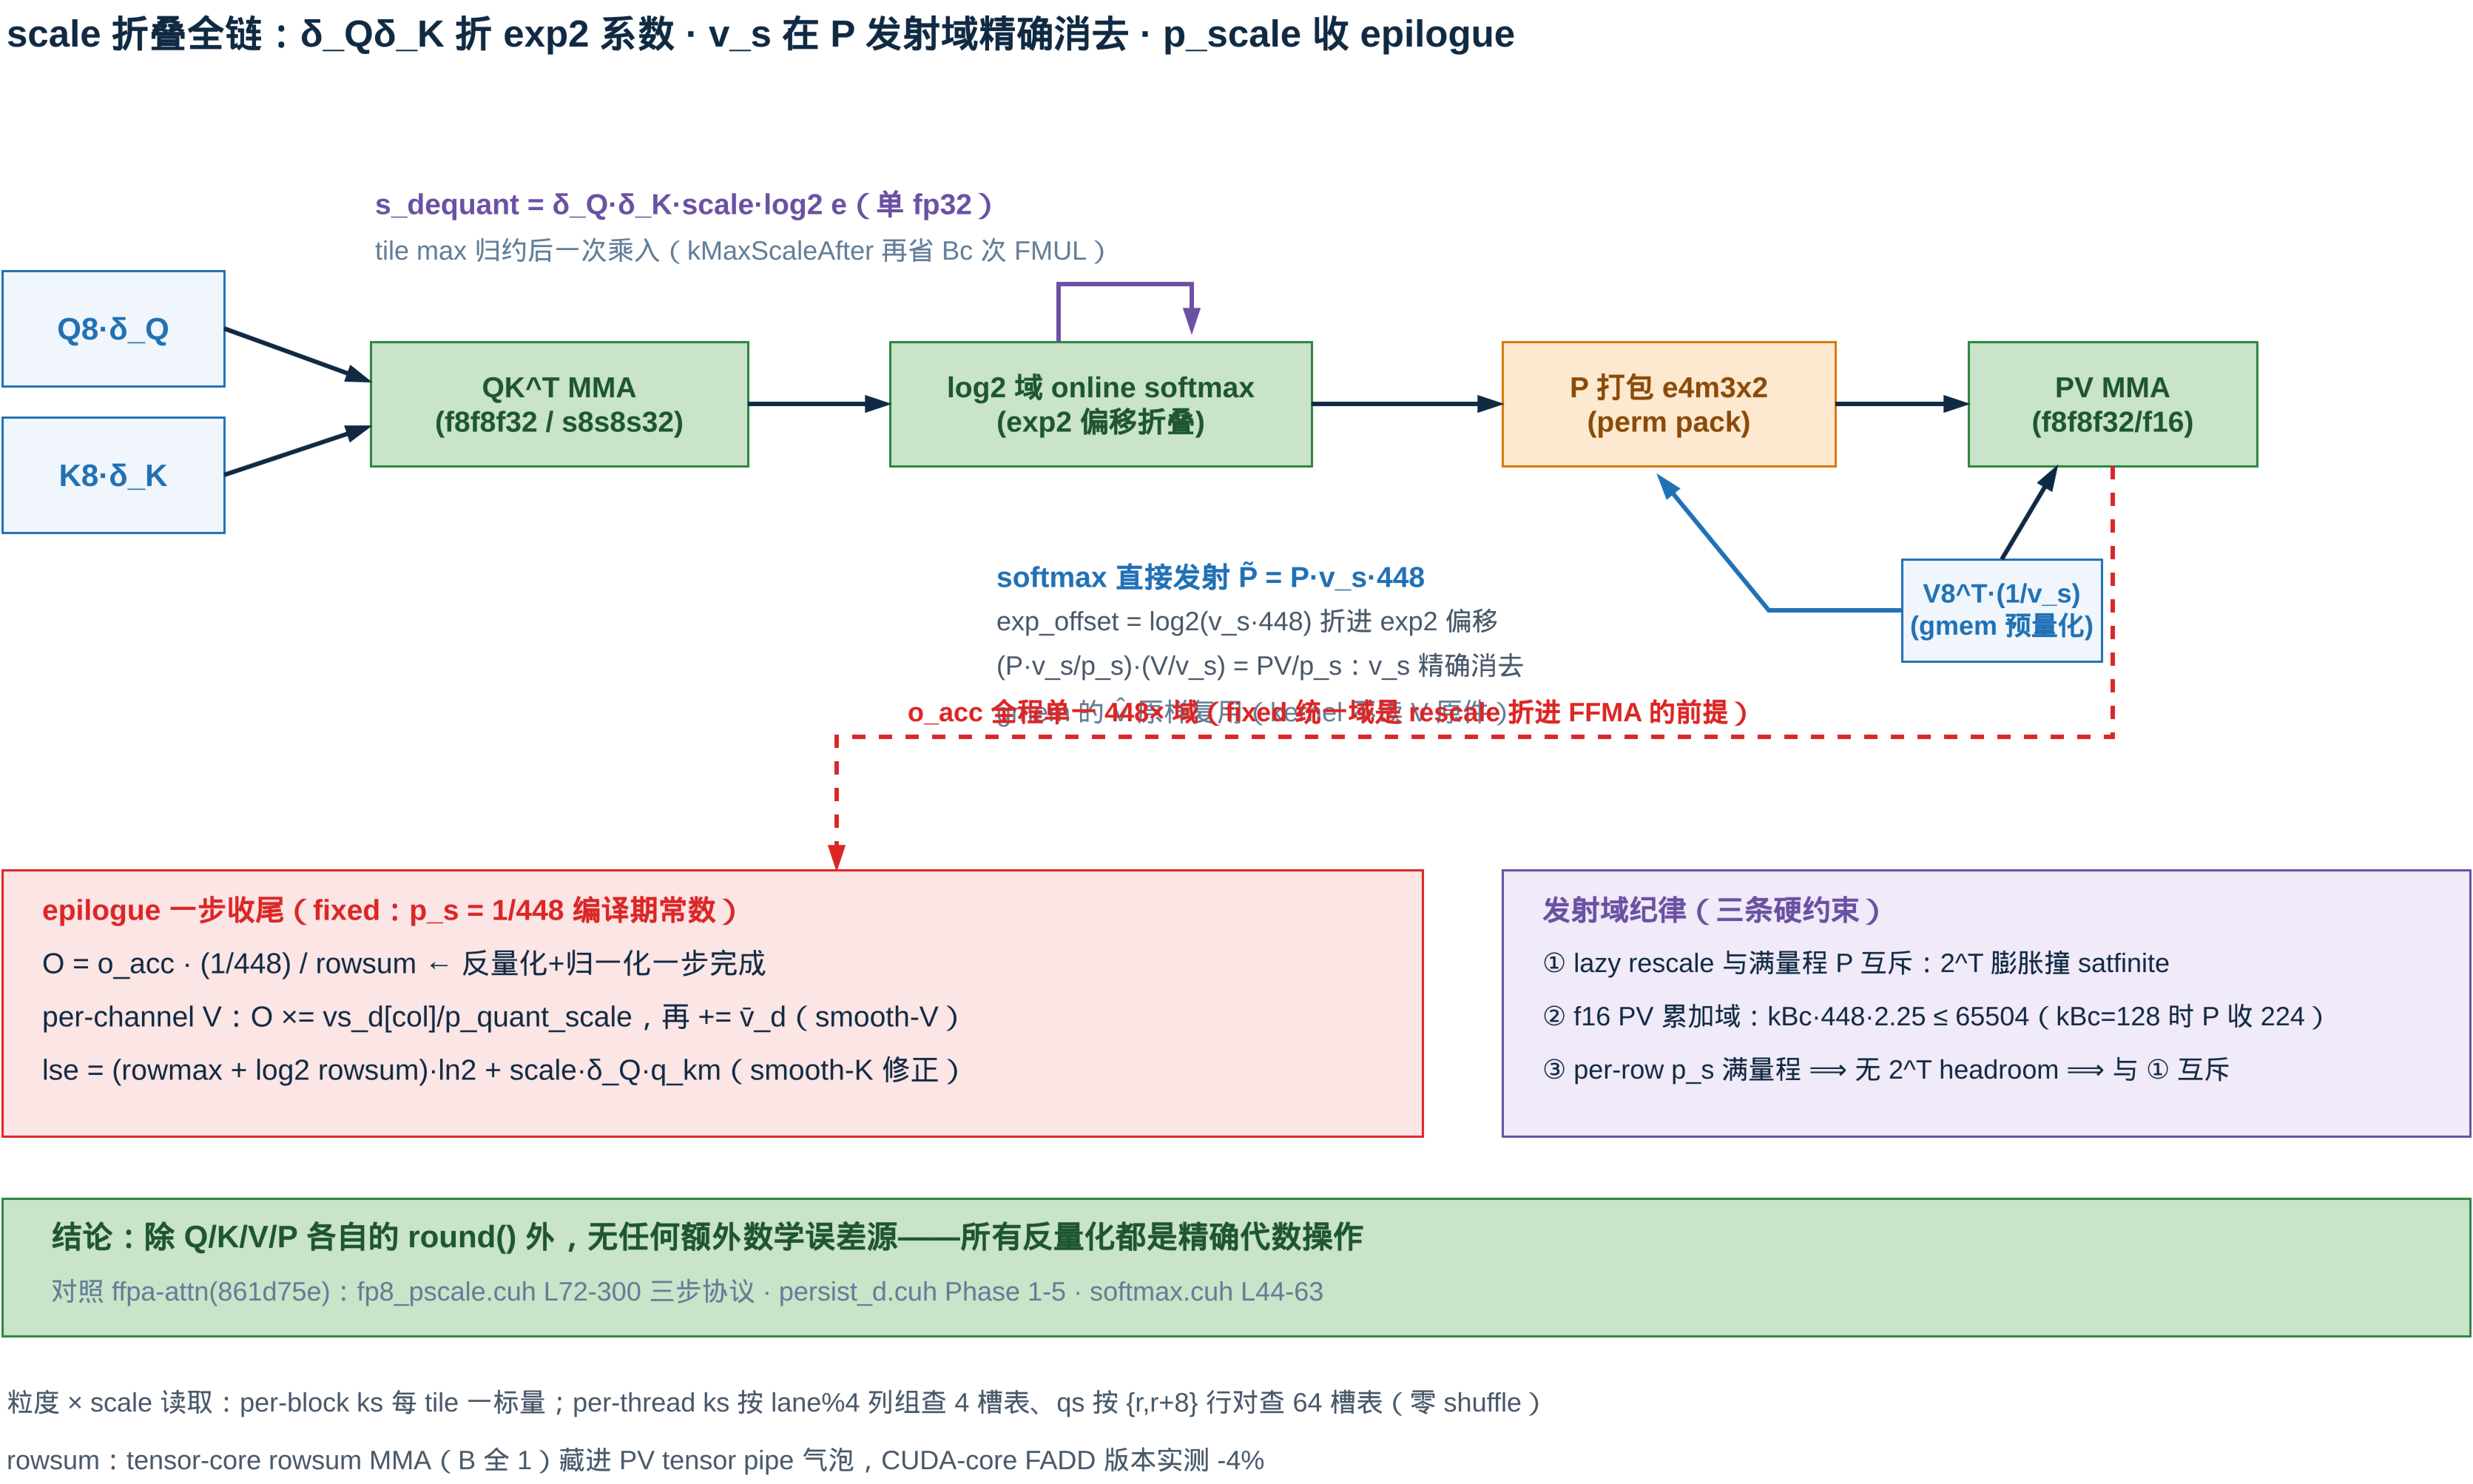
\includegraphics[width=0.98\textwidth]{figures/drawio/fig-29-1-scale-folding/fig-29-1-scale-folding.png}
  \begin{tikzpicture}
    \node[anchor=west, inner sep=0pt, align=left, font={\fontsize{7.4}{9.3}\selectfont \bfseries }] at (0.37,-0.354) {scale 折叠全链：$\delta$\_Q$\delta$\_K 折 exp2 系数 $\cdot$ v\_s 在未舍入代数中消去 $\cdot$ p\_scale 收 epilogue};% w=17.125
    \node[draw=tkBlue, fill=tkFillBlue, line width=0.5pt, minimum width=1.54cm, minimum height=0.80cm, inner sep=1pt, align=center, text width=1.48cm, font={\fontsize{6.1}{7.7}\selectfont \bfseries \color{tkBlue} }] at (1.14,-2.402) {Q8$\cdot$$\delta$\_Q};
    \node[draw=tkBlue, fill=tkFillBlue, line width=0.5pt, minimum width=1.54cm, minimum height=0.80cm, inner sep=1pt, align=center, text width=1.48cm, font={\fontsize{6.1}{7.7}\selectfont \bfseries \color{tkBlue} }] at (1.14,-3.419) {K8$\cdot$$\delta$\_K};
    \node[draw=tkGreen, fill=tkFillGreen, line width=0.5pt, minimum width=2.62cm, minimum height=0.86cm, inner sep=1pt, align=center, text width=2.56cm, font={\fontsize{5.7}{7.1}\selectfont \bfseries \color{tkGreen!70!black} }] at (4.235,-2.926) {QK\^{}T MMA\\(f8f8f32 / s8s8s32)};
    \node[draw=tkGreen, fill=tkFillGreen, line width=0.5pt, minimum width=2.93cm, minimum height=0.86cm, inner sep=1pt, align=center, text width=2.86cm, font={\fontsize{5.7}{7.1}\selectfont \bfseries \color{tkGreen!70!black} }] at (7.993,-2.926) {log2 域 online softmax\\(exp2 偏移折叠)};
    \node[draw=tkOrange, fill=tkFillOrange, line width=0.5pt, minimum width=2.31cm, minimum height=0.86cm, inner sep=1pt, align=center, text width=2.25cm, font={\fontsize{5.7}{7.1}\selectfont \bfseries \color{tkOrange!75!black} }] at (11.935,-2.926) {P 打包 e4m3x2\\(perm pack)};
    \node[draw=tkGreen, fill=tkFillGreen, line width=0.5pt, minimum width=2.00cm, minimum height=0.86cm, inner sep=1pt, align=center, text width=1.94cm, font={\fontsize{5.7}{7.1}\selectfont \bfseries \color{tkGreen!70!black} }] at (15.015,-2.926) {PV MMA\\(f8f8f32/f16)};
    \node[draw=tkBlue, fill=tkFillBlue, line width=0.5pt, minimum width=1.39cm, minimum height=0.71cm, inner sep=1pt, align=center, text width=1.32cm, font={\fontsize{4.1}{5.1}\selectfont \bfseries \color{tkBlue} }] at (14.245,-4.358) {V8\^{}T$\cdot$(1/v\_s)\\(gmem 预量化)};
    \node[anchor=west, inner sep=0pt, align=left, font={\fontsize{5.7}{7.1}\selectfont \bfseries \color{tkPurple} }] at (2.926,-1.54) {s\_dequant = $\delta$\_Q$\cdot$$\delta$\_K$\cdot$scale$\cdot$log2 e（单 fp32）};% w=5.852
    \node[anchor=west, inner sep=0pt, align=left, font={\fontsize{4.8}{6.0}\selectfont \color{black!55} }] at (2.926,-1.863) {per-block：tile max 后乘入；per-thread：先乘 q\_s k\_s};% w=5.852
    \node[anchor=west, inner sep=0pt, align=left, font={\fontsize{5.7}{7.1}\selectfont \bfseries \color{tkBlue} }] at (7.238,-4.127) {softmax 直接发射 $\tilde{P}$ = P$\cdot$v\_s$\cdot$448};% w=5.082
    \node[anchor=west, inner sep=0pt, align=left, font={\fontsize{5.2}{6.6}\selectfont \color{black!65} }] at (7.238,-4.435) {exp\_offset = log2(v\_s$\cdot$448) 折进 exp2 偏移};% w=5.236
    \node[anchor=west, inner sep=0pt, align=left, font={\fontsize{5.2}{6.6}\selectfont \color{black!65} }] at (7.238,-4.743) {(P$\cdot$v\_s/p\_s)$\cdot$(V/v\_s) = PV/p\_s：未舍入代数中 v\_s 消去};% w=5.236
    \node[anchor=west, inner sep=0pt, align=left, font={\fontsize{5.2}{6.6}\selectfont \color{black!55} }] at (7.238,-5.067) {gmem 的 $\hat{V}$ 原样复用（kernel 不读 V 原件）};% w=5.544
    \node[draw=tkRed, fill=tkFillRed, line width=0.5pt, minimum width=9.86cm, minimum height=1.85cm, inner sep=1pt, align=center, text width=9.79cm, font={\fontsize{5.7}{7.1}\selectfont }] at (5.298,-7.084) {};
    \node[anchor=west, inner sep=0pt, align=left, font={\fontsize{5.7}{7.1}\selectfont \bfseries \color{tkRed} }] at (0.616,-6.437) {epilogue 一步收尾（fixed：p\_s = 1/448 编译期常数）};% w=9.363
    \node[anchor=west, inner sep=0pt, align=left, font={\fontsize{5.7}{7.1}\selectfont }] at (0.616,-6.807) {O = o\_acc $\cdot$ (1/448) / rowsum        $\leftarrow$ 反量化+归一化一步完成};% w=9.363
    \node[anchor=west, inner sep=0pt, align=left, font={\fontsize{5.7}{7.1}\selectfont }] at (0.616,-7.176) {per-channel V：O $\times$= vs\_d[col]/p\_quant\_scale，再 += $\bar{v}$\_d（smooth-V）};% w=9.363
    \node[anchor=west, inner sep=0pt, align=left, font={\fontsize{5.7}{7.1}\selectfont }] at (0.616,-7.546) {lse = (rowmax + log2 rowsum)$\cdot$ln2  +  scale$\cdot$$\delta$\_Q$\cdot$q\_km（smooth-K 修正）};% w=9.363
    \node[anchor=west, inner sep=0pt, align=left, font={\fontsize{4.6}{5.8}\selectfont \bfseries \color{tkRed} }] at (6.622,-5.452) {o\_acc 全程单一 448$\times$ 域（fixed 统一域是 rescale 折进 FFMA 的前提）};% w=6.468
    \node[draw=tkPurple, fill=tkFillPurple, line width=0.5pt, minimum width=6.71cm, minimum height=1.85cm, inner sep=1pt, align=center, text width=6.65cm, font={\fontsize{5.7}{7.1}\selectfont }] at (14.137,-7.084) {};
    \node[anchor=west, inner sep=0pt, align=left, font={\fontsize{5.7}{7.1}\selectfont \bfseries \color{tkPurple} }] at (11.026,-6.437) {发射域规则（三条硬约束）};% w=6.222
    \node[anchor=west, inner sep=0pt, align=left, font={\fontsize{5.2}{6.6}\selectfont }] at (11.026,-6.807) {(1) lazy rescale 与满量程 P 互斥：2\^{}T 膨胀撞 satfinite};% w=6.222
    \node[anchor=west, inner sep=0pt, align=left, font={\fontsize{4.6}{5.8}\selectfont }] at (11.026,-7.176) {(2) f16 PV 累加域：kBc$\cdot$448$\cdot$2.25 $\leq$ 65504（kBc=128 时 P 收 224）};% w=6.222
    \node[anchor=west, inner sep=0pt, align=left, font={\fontsize{5.2}{6.6}\selectfont }] at (11.026,-7.546) {(3) per-row p\_s 满量程 $\Longrightarrow$ 无 2\^{}T headroom $\Longrightarrow$ 与 (1) 互斥};% w=6.222
    \node[draw=tkGreen, fill=tkFillGreen, line width=0.5pt, minimum width=17.12cm, minimum height=0.95cm, inner sep=1pt, align=center, text width=17.06cm, font={\fontsize{5.7}{7.1}\selectfont }] at (8.932,-8.917) {};
    \node[anchor=west, inner sep=0pt, align=left, font={\fontsize{6.1}{7.7}\selectfont \bfseries \color{tkGreen!70!black} }] at (0.678,-8.701) {结论：实数代数下除 Q/K/V/P 的 round() 外无额外误差源；浮点执行仍有乘加、exp2 与累加舍入};% w=16.509
    \node[anchor=west, inner sep=0pt, align=left, font={\fontsize{5.2}{6.6}\selectfont \color{black!55} }] at (0.678,-9.086) {对照 ffpa-attn(861d75e)：fp8\_pscale.cuh L72-300 三步协议 $\cdot$ persist\_d.cuh Phase 1-5 $\cdot$ softmax.cuh L44-63};% w=16.509
    \node[anchor=west, inner sep=0pt, align=left, font={\fontsize{5.2}{6.6}\selectfont \color{black!65} }] at (0.37,-9.856) {粒度 $\times$ scale 读取：per-block ks 每 tile 一标量；per-thread ks 按 lane\%4 列组查 4 槽表、qs 按 {r,r+8} 行对查 64 槽表（零 shuffle）};% w=17.125
    \node[anchor=west, inner sep=0pt, align=left, font={\fontsize{5.2}{6.6}\selectfont \color{black!65} }] at (0.37,-10.256) {rowsum：tensor-core rowsum MMA（B 全 1）藏进 PV tensor pipe 气泡，CUDA-core FADD 版本实测 -4\%};% w=17.125
    \draw[black!75, line width=0.8pt, -{Stealth[length=2.2pt,width=1.8pt]}] (1.91,-2.402) -- (2.926,-2.772);
    \draw[black!75, line width=0.8pt, -{Stealth[length=2.2pt,width=1.8pt]}] (1.91,-3.419) -- (2.926,-3.08);
    \draw[black!75, line width=0.8pt, -{Stealth[length=2.2pt,width=1.8pt]}] (5.544,-2.926) -- (6.53,-2.926);
    \draw[black!75, line width=0.8pt, -{Stealth[length=2.2pt,width=1.8pt]}] (9.456,-2.926) -- (10.78,-2.926);
    \draw[black!75, line width=0.8pt, -{Stealth[length=2.2pt,width=1.8pt]}] (13.09,-2.926) -- (14.014,-2.926);
    \draw[black!75, line width=0.8pt, -{Stealth[length=2.2pt,width=1.8pt]}] (14.245,-4.004) -- (14.63,-3.357);
    \draw[tkPurple, line width=0.8pt, -{Stealth[length=2.2pt,width=1.8pt]}] (7.7,-2.495) -- (7.7,-2.094) -- (8.624,-2.094) -- (8.624,-2.433);
    \draw[tkBlue, line width=0.8pt, -{Stealth[length=2.2pt,width=1.8pt]}] (13.552,-4.358) -- (12.628,-4.358) -- (11.858,-3.419);
    \draw[tkRed, line width=0.8pt, dashed, -{Stealth[length=2.2pt,width=1.8pt]}] (15.015,-3.357) -- (15.015,-5.236) -- (6.16,-5.236) -- (6.16,-6.16);
  \end{tikzpicture}
  \caption{scale 折叠全链数据流：$\delta_Q\delta_K$ 折进 exp2 系数、$v_s$
  在 P 发射域消去、$p_{scale}$ 收在 epilogue——实数代数下除 round() 外无额外
  误差源；浮点执行仍有乘加、exp2 与累加舍入。}
  \label{fig:29-scale-folding}
\end{figure}

\begin{figure}[htbp]
  \centering
  % was: 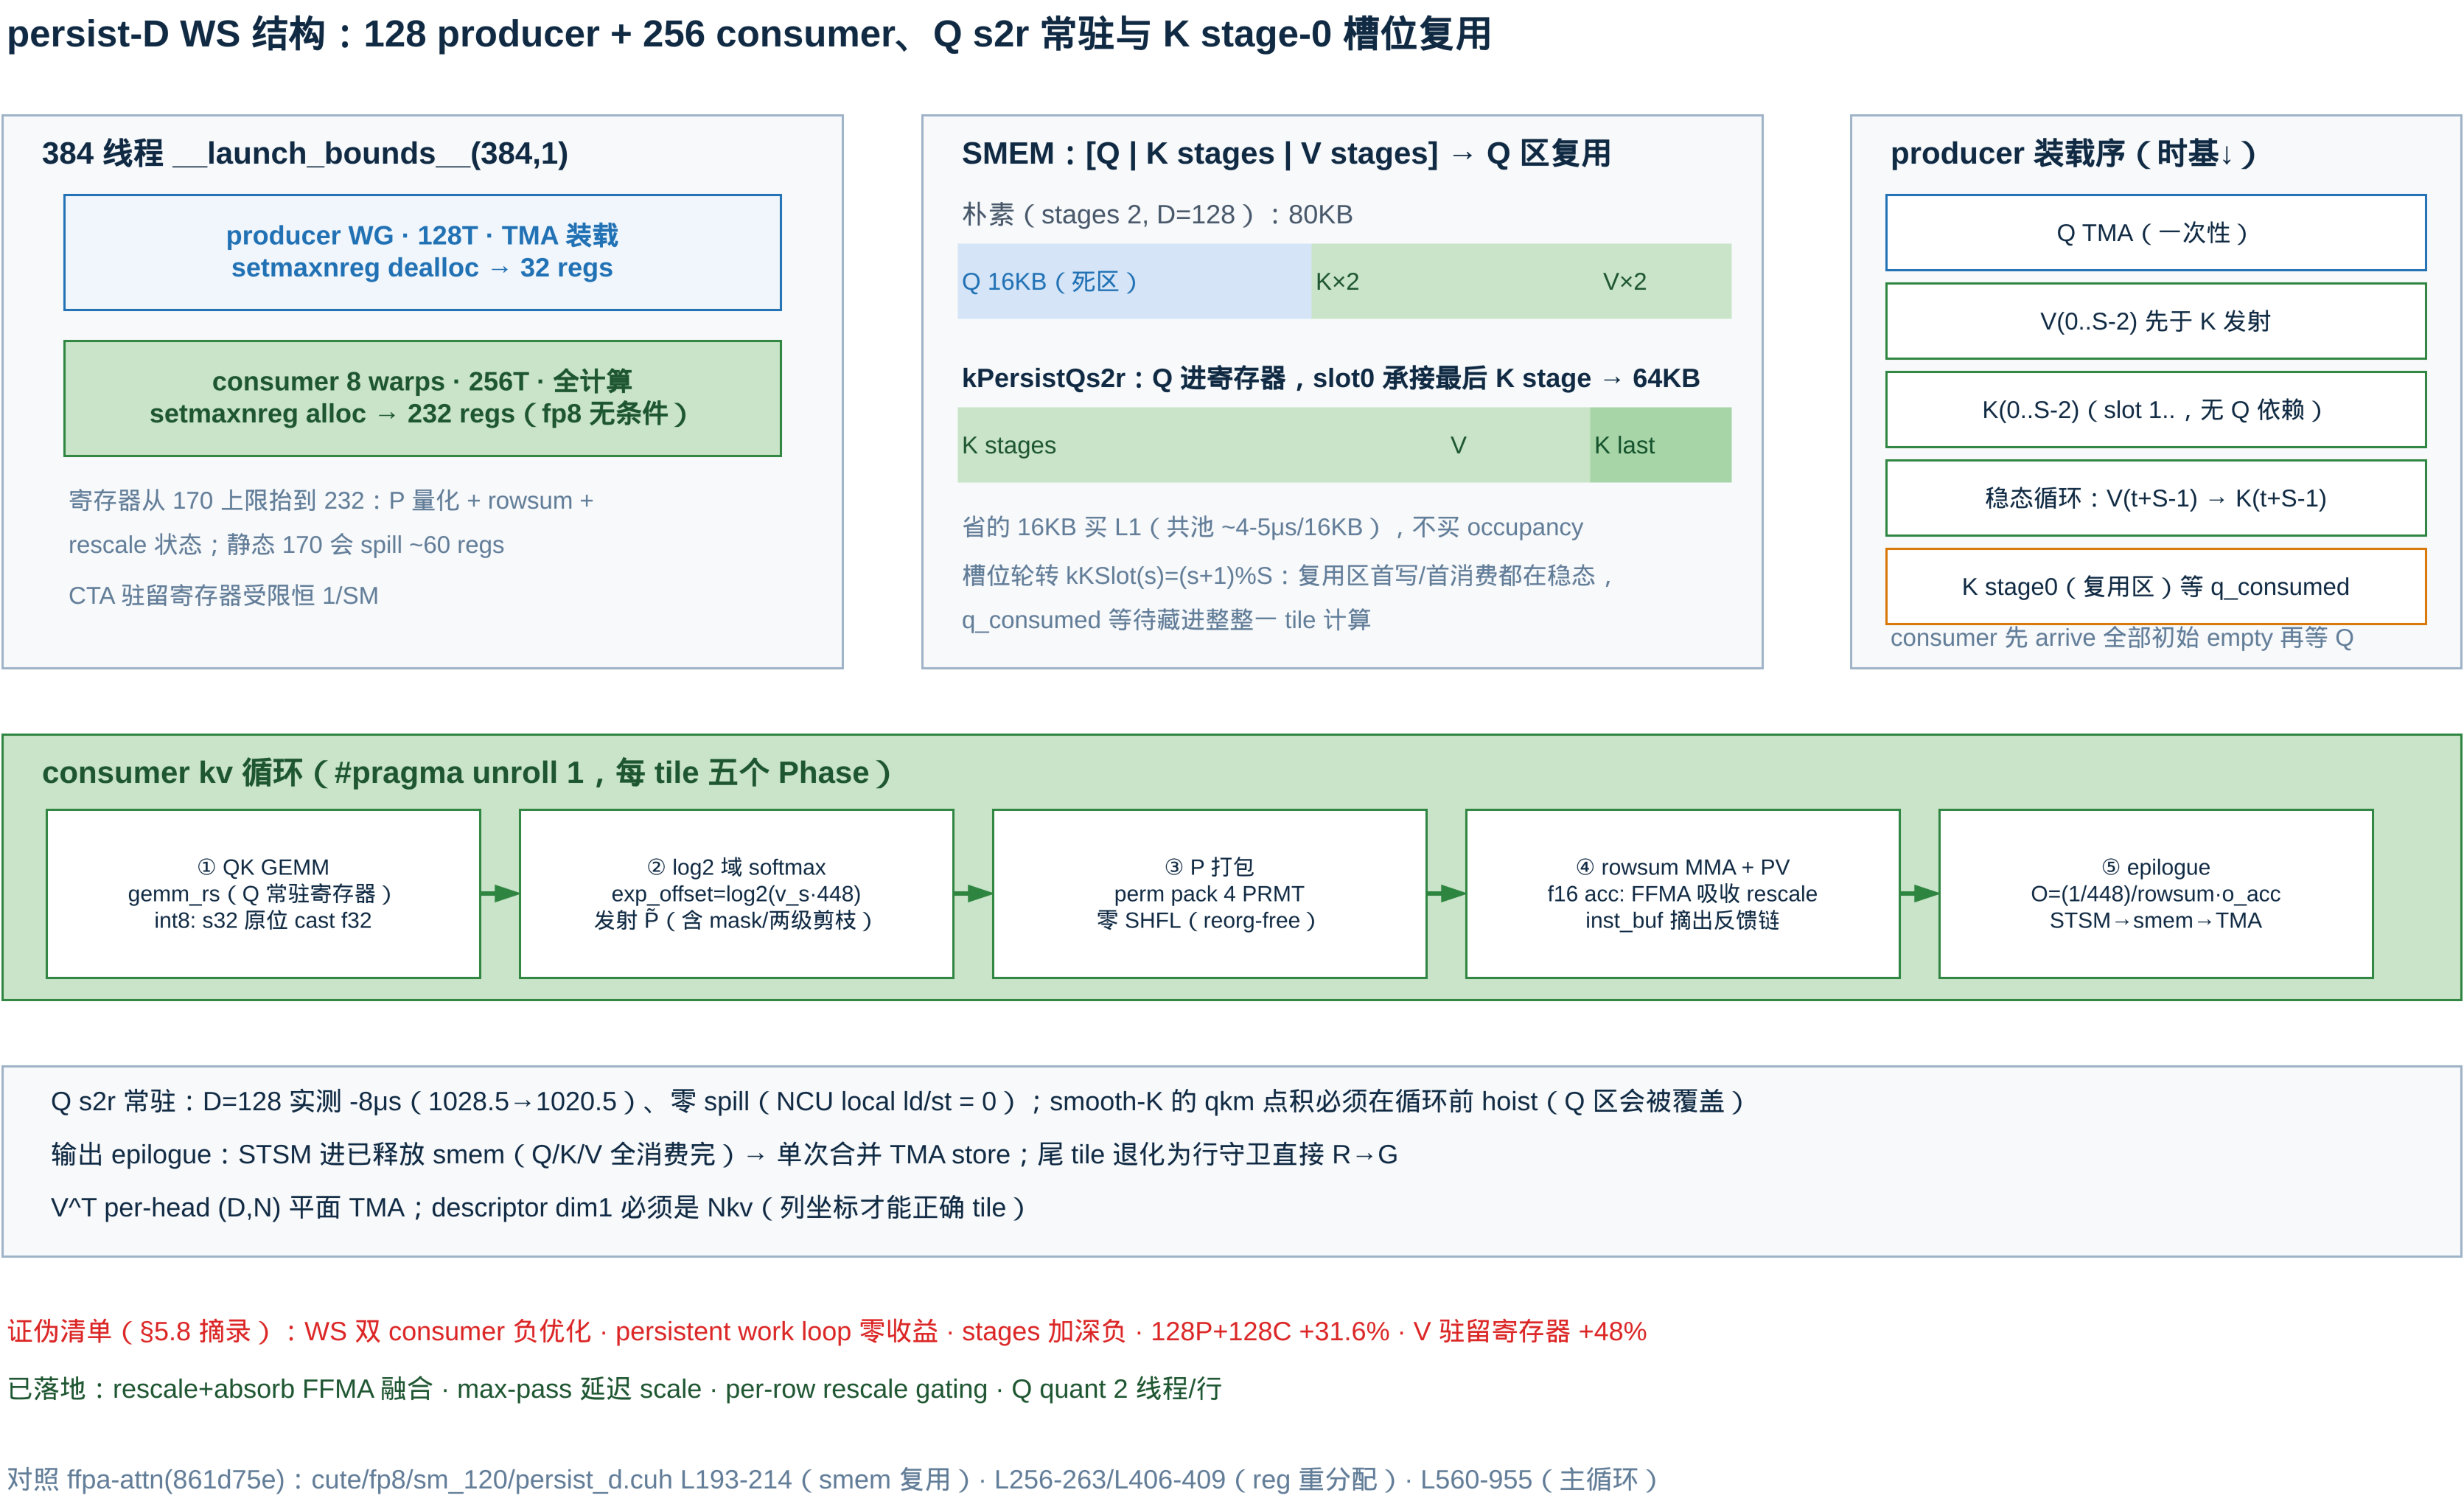
\includegraphics[width=0.98\textwidth]{figures/drawio/fig-29-2-persist-d-ws/fig-29-2-persist-d-ws.png}
  \begin{tikzpicture}
    \node[anchor=west, inner sep=0pt, align=left, font={\fontsize{7.4}{9.3}\selectfont \bfseries }] at (0.37,-0.354) {persist-D WS 结构：128 producer + 256 consumer、Q s2r 常驻与 K stage-0 槽位复用};% w=17.125
    \node[draw=gray!55, fill=black!3, line width=0.5pt, minimum width=5.85cm, minimum height=3.85cm, inner sep=1pt, align=center, text width=5.79cm, font={\fontsize{5.7}{7.1}\selectfont }] at (3.296,-2.849) {};
    \node[anchor=west, inner sep=0pt, align=left, font={\fontsize{6.1}{7.7}\selectfont \bfseries }] at (0.616,-1.186) {384 线程 \_\_launch\_bounds\_\_(384,1)};% w=5.359
    \node[draw=tkBlue, fill=tkFillBlue, line width=0.5pt, minimum width=4.99cm, minimum height=0.80cm, inner sep=1pt, align=center, text width=4.93cm, font={\fontsize{5.2}{6.6}\selectfont \bfseries \color{tkBlue} }] at (3.296,-1.879) {producer WG $\cdot$ 128T $\cdot$ TMA 装载\\setmaxnreg dealloc $\to$ 32 regs};
    \node[draw=tkGreen, fill=tkFillGreen, line width=0.5pt, minimum width=4.99cm, minimum height=0.80cm, inner sep=1pt, align=center, text width=4.93cm, font={\fontsize{5.2}{6.6}\selectfont \bfseries \color{tkGreen!70!black} }] at (3.296,-2.895) {consumer 8 warps $\cdot$ 256T $\cdot$ 全计算\\setmaxnreg alloc $\to$ 232 regs（fp8 无条件）};
    \node[anchor=west, inner sep=0pt, align=left, font={\fontsize{4.8}{6.0}\selectfont \color{black!55} }] at (0.801,-3.604) {寄存器从 170 上限抬到 232：P 量化 + rowsum +};% w=4.990
    \node[anchor=west, inner sep=0pt, align=left, font={\fontsize{4.8}{6.0}\selectfont \color{black!55} }] at (0.801,-3.912) {rescale 状态；静态 170 会 spill \textasciitilde{}60 regs};% w=4.990
    \node[anchor=west, inner sep=0pt, align=left, font={\fontsize{4.8}{6.0}\selectfont \color{black!55} }] at (0.801,-4.266) {CTA 驻留寄存器受限恒 1/SM};% w=4.990
    \node[draw=gray!55, fill=black!3, line width=0.5pt, minimum width=5.85cm, minimum height=3.85cm, inner sep=1pt, align=center, text width=5.79cm, font={\fontsize{5.7}{7.1}\selectfont }] at (9.702,-2.849) {};
    \node[anchor=west, inner sep=0pt, align=left, font={\fontsize{5.7}{7.1}\selectfont \bfseries }] at (7.022,-1.186) {SMEM：[Q | K stages | V stages] $\to$ Q 区复用};% w=5.359
    \node[anchor=west, inner sep=0pt, align=left, font={\fontsize{5.2}{6.6}\selectfont \color{black!65} }] at (7.022,-1.617) {朴素（stages 2, D=128）：80KB};% w=5.359
    \node[draw=none, fill=tkFillBlue, line width=0.5pt, minimum width=2.46cm, minimum height=0.52cm, inner sep=1pt, align=center, text width=2.40cm, font={\fontsize{5.7}{7.1}\selectfont \color{tkBlue} }] at (8.254,-2.079) {};
    \node[draw=none, fill=tkFillGreen, line width=0.5pt, minimum width=2.00cm, minimum height=0.52cm, inner sep=1pt, align=center, text width=1.94cm, font={\fontsize{5.7}{7.1}\selectfont \color{tkBlue} }] at (10.487,-2.079) {};
    \node[draw=none, fill=tkFillGreen, line width=0.5pt, minimum width=0.92cm, minimum height=0.52cm, inner sep=1pt, align=center, text width=0.86cm, font={\fontsize{5.7}{7.1}\selectfont \color{tkBlue} }] at (11.95,-2.079) {};
    \node[anchor=west, inner sep=0pt, align=left, font={\fontsize{4.8}{6.0}\selectfont \color{tkBlue} }] at (7.022,-2.079) {Q 16KB（死区）};% w=2.464
    \node[anchor=west, inner sep=0pt, align=left, font={\fontsize{4.8}{6.0}\selectfont \color{tkGreen!70!black} }] at (9.486,-2.079) {K$\times$2};% w=2.002
    \node[anchor=west, inner sep=0pt, align=left, font={\fontsize{4.8}{6.0}\selectfont \color{tkGreen!70!black} }] at (11.488,-2.079) {V$\times$2};% w=0.924
    \node[anchor=west, inner sep=0pt, align=left, font={\fontsize{4.3}{5.3}\selectfont \bfseries }] at (7.022,-2.757) {kPersistQs2r：Q 进寄存器，slot0 承接最后 K stage $\to$ 64KB};% w=5.359
    \node[draw=none, fill=tkFillGreen, line width=0.5pt, minimum width=3.40cm, minimum height=0.52cm, inner sep=1pt, align=center, text width=3.34cm, font={\fontsize{5.7}{7.1}\selectfont \color{tkBlue} }] at (8.724,-3.219) {};
    \node[draw=none, fill=tkFillGreen, line width=0.5pt, minimum width=1.00cm, minimum height=0.52cm, inner sep=1pt, align=center, text width=0.94cm, font={\fontsize{5.7}{7.1}\selectfont \color{tkBlue} }] at (10.926,-3.219) {};
    \node[draw=none, fill=tkFillGreen, line width=0.5pt, minimum width=0.99cm, minimum height=0.52cm, inner sep=1pt, align=center, text width=0.92cm, font={\fontsize{5.7}{7.1}\selectfont \color{tkBlue} }] at (11.92,-3.219) {};
    \node[anchor=west, inner sep=0pt, align=left, font={\fontsize{4.8}{6.0}\selectfont \color{tkGreen!70!black} }] at (7.022,-3.219) {K stages};% w=3.403
    \node[anchor=west, inner sep=0pt, align=left, font={\fontsize{4.8}{6.0}\selectfont \color{tkGreen!70!black} }] at (10.426,-3.219) {V};% w=1.001
    \node[anchor=west, inner sep=0pt, align=left, font={\fontsize{4.8}{6.0}\selectfont \color{tkGreen!70!black} }] at (11.427,-3.219) {K last};% w=0.986
    \node[anchor=west, inner sep=0pt, align=left, font={\fontsize{4.8}{6.0}\selectfont \color{black!55} }] at (7.022,-3.788) {省的 16KB 换 L1（共池 \textasciitilde{}4-5$\mu$s/16KB），不换 occupancy};% w=5.359
    \node[anchor=west, inner sep=0pt, align=left, font={\fontsize{4.8}{6.0}\selectfont \color{black!55} }] at (7.022,-4.127) {槽位轮转 kKSlot(s)=(s+1)\%S：复用区首写/首消费都在稳态，};% w=5.359
    \node[anchor=west, inner sep=0pt, align=left, font={\fontsize{4.8}{6.0}\selectfont \color{black!55} }] at (7.022,-4.435) {q\_consumed 等待藏进整整一 tile 计算};% w=5.359
    \node[draw=gray!55, fill=black!3, line width=0.5pt, minimum width=4.25cm, minimum height=3.85cm, inner sep=1pt, align=center, text width=4.19cm, font={\fontsize{5.7}{7.1}\selectfont }] at (15.369,-2.849) {};
    \node[anchor=west, inner sep=0pt, align=left, font={\fontsize{6.1}{7.7}\selectfont \bfseries }] at (13.49,-1.186) {producer 装载序（时基$\downarrow$）};% w=3.758
    \node[draw=tkBlue, fill=none, line width=0.5pt, minimum width=3.76cm, minimum height=0.52cm, inner sep=1pt, align=center, text width=3.70cm, font={\fontsize{4.8}{6.0}\selectfont }] at (15.369,-1.74) {Q TMA（一次性）};
    \node[draw=tkGreen, fill=none, line width=0.5pt, minimum width=3.76cm, minimum height=0.52cm, inner sep=1pt, align=center, text width=3.70cm, font={\fontsize{4.8}{6.0}\selectfont }] at (15.369,-2.356) {V(0..S-2) 先于 K 发射};
    \node[draw=tkGreen, fill=none, line width=0.5pt, minimum width=3.76cm, minimum height=0.52cm, inner sep=1pt, align=center, text width=3.70cm, font={\fontsize{4.8}{6.0}\selectfont }] at (15.369,-2.972) {K(0..S-2)（slot 1..，无 Q 依赖）};
    \node[draw=tkGreen, fill=none, line width=0.5pt, minimum width=3.76cm, minimum height=0.52cm, inner sep=1pt, align=center, text width=3.70cm, font={\fontsize{4.8}{6.0}\selectfont }] at (15.369,-3.588) {稳态循环：V(t+S-1) $\to$ K(t+S-1)};
    \node[draw=tkOrange, fill=none, line width=0.5pt, minimum width=3.76cm, minimum height=0.52cm, inner sep=1pt, align=center, text width=3.70cm, font={\fontsize{4.8}{6.0}\selectfont }] at (15.369,-4.204) {K stage0（复用区）等 q\_consumed};
    \node[anchor=west, inner sep=0pt, align=left, font={\fontsize{4.5}{5.6}\selectfont \color{black!55} }] at (13.49,-4.558) {consumer 先 arrive 全部初始 empty 再等 Q};% w=3.758
    \node[draw=tkGreen, fill=tkFillGreen, line width=0.5pt, minimum width=17.12cm, minimum height=1.85cm, inner sep=1pt, align=center, text width=17.06cm, font={\fontsize{5.7}{7.1}\selectfont }] at (8.932,-6.16) {};
    \node[anchor=west, inner sep=0pt, align=left, font={\fontsize{6.1}{7.7}\selectfont \bfseries \color{tkGreen!70!black} }] at (0.616,-5.498) {consumer kv 循环（\#pragma unroll 1，每 tile 五个 Phase）};% w=16.509
    \node[draw=tkGreen, fill=none, line width=0.5pt, minimum width=3.02cm, minimum height=1.17cm, inner sep=1pt, align=center, text width=2.96cm, font={\fontsize{4.4}{5.5}\selectfont }] at (2.187,-6.345) {(1) QK GEMM\\gemm\_rs（Q 常驻寄存器）\\int8: s32 原位 cast f32};
    \node[draw=tkGreen, fill=none, line width=0.5pt, minimum width=3.02cm, minimum height=1.17cm, inner sep=1pt, align=center, text width=2.96cm, font={\fontsize{4.4}{5.5}\selectfont }] at (5.482,-6.345) {(2) log2 域 softmax\\exp\_offset=log2(v\_s$\cdot$448)\\发射 $\tilde{P}$（含 mask/两级剪枝）};
    \node[draw=tkGreen, fill=none, line width=0.5pt, minimum width=3.02cm, minimum height=1.17cm, inner sep=1pt, align=center, text width=2.96cm, font={\fontsize{4.4}{5.5}\selectfont }] at (8.778,-6.345) {(3) P 打包\\每 K32 组 4 PRMT\\零 SHFL（reorg-free）};
    \node[draw=tkGreen, fill=none, line width=0.5pt, minimum width=3.02cm, minimum height=1.17cm, inner sep=1pt, align=center, text width=2.96cm, font={\fontsize{4.4}{5.5}\selectfont }] at (12.074,-6.345) {(4) rowsum MMA + PV\\f16 acc: FFMA 吸收 rescale\\inst\_buf 摘出反馈链};
    \node[draw=tkGreen, fill=none, line width=0.5pt, minimum width=3.02cm, minimum height=1.17cm, inner sep=1pt, align=center, text width=2.96cm, font={\fontsize{4.4}{5.5}\selectfont }] at (15.369,-6.345) {(5) epilogue\\O=(1/448)/rowsum$\cdot$o\_acc\\STSM$\to$smem$\to$TMA};
    \node[draw=gray!55, fill=black!3, line width=0.5pt, minimum width=17.12cm, minimum height=1.32cm, inner sep=1pt, align=center, text width=17.06cm, font={\fontsize{5.7}{7.1}\selectfont }] at (8.932,-8.208) {};
    \node[anchor=west, inner sep=0pt, align=left, font={\fontsize{5.2}{6.6}\selectfont }] at (0.678,-7.792) {Q s2r 常驻：D=128 实测 -8$\mu$s（1028.5$\to$1020.5）、零 spill（NCU local ld/st = 0）；smooth-K 的 qkm 点积必须在循环前 hoist（Q 区会被覆盖）};% w=16.509
    \node[anchor=west, inner sep=0pt, align=left, font={\fontsize{5.2}{6.6}\selectfont }] at (0.678,-8.162) {输出 epilogue：STSM 进已释放 smem（Q/K/V 全消费完）$\to$ 单次合并 TMA store；尾 tile 退化为行守卫直接 R$\to$G};% w=16.509
    \node[anchor=west, inner sep=0pt, align=left, font={\fontsize{5.2}{6.6}\selectfont }] at (0.678,-8.532) {V\^{}T per-head (D,N) 平面 TMA；descriptor dim1 必须是 Nkv（列坐标才能正确 tile）};% w=16.509
    \node[anchor=west, inner sep=0pt, align=left, font={\fontsize{5.2}{6.6}\selectfont \color{tkRed} }] at (0.37,-9.394) {证伪清单（\S{}5.8 摘录）：WS 双 consumer 负优化 $\cdot$ persistent work loop 零收益 $\cdot$ stages 加深负 $\cdot$ 128P+128C +31.6\% $\cdot$ V 驻留寄存器 +48\%};% w=17.125
    \node[anchor=west, inner sep=0pt, align=left, font={\fontsize{5.2}{6.6}\selectfont \color{tkGreen!70!black} }] at (0.37,-9.794) {已落地：rescale+absorb FFMA 融合 $\cdot$ max-pass 延迟 scale $\cdot$ per-row rescale gating $\cdot$ Q quant 2 线程/行};% w=17.125
    \node[anchor=west, inner sep=0pt, align=left, font={\fontsize{5.2}{6.6}\selectfont \color{black!55} }] at (0.37,-10.426) {对照 ffpa-attn(861d75e)：cute/fp8/sm\_120/persist\_d.cuh L193-214（smem 复用）$\cdot$ L256-263/L406-409（reg 重分配）$\cdot$ L560-955（主循环）};% w=17.125
    \draw[tkGreen, line width=0.8pt, -{Stealth[length=2.2pt,width=1.8pt]}] (3.696,-6.345) -- (3.973,-6.345);
    \draw[tkGreen, line width=0.8pt, -{Stealth[length=2.2pt,width=1.8pt]}] (6.992,-6.345) -- (7.269,-6.345);
    \draw[tkGreen, line width=0.8pt, -{Stealth[length=2.2pt,width=1.8pt]}] (10.287,-6.345) -- (10.564,-6.345);
    \draw[tkGreen, line width=0.8pt, -{Stealth[length=2.2pt,width=1.8pt]}] (13.583,-6.345) -- (13.86,-6.345);
  \end{tikzpicture}
  \caption{persist-D WS 结构：128P+256C、setmaxnreg 32/232、Q s2r 常驻与
  K 槽位 0（Q 区）复用给最后一个 K stage 的 smem 复用、STSM+TMA 输出。}
  \label{fig:29-persist-d-ws}
\end{figure}

\begin{figure}[htbp]
  \centering
  % was: 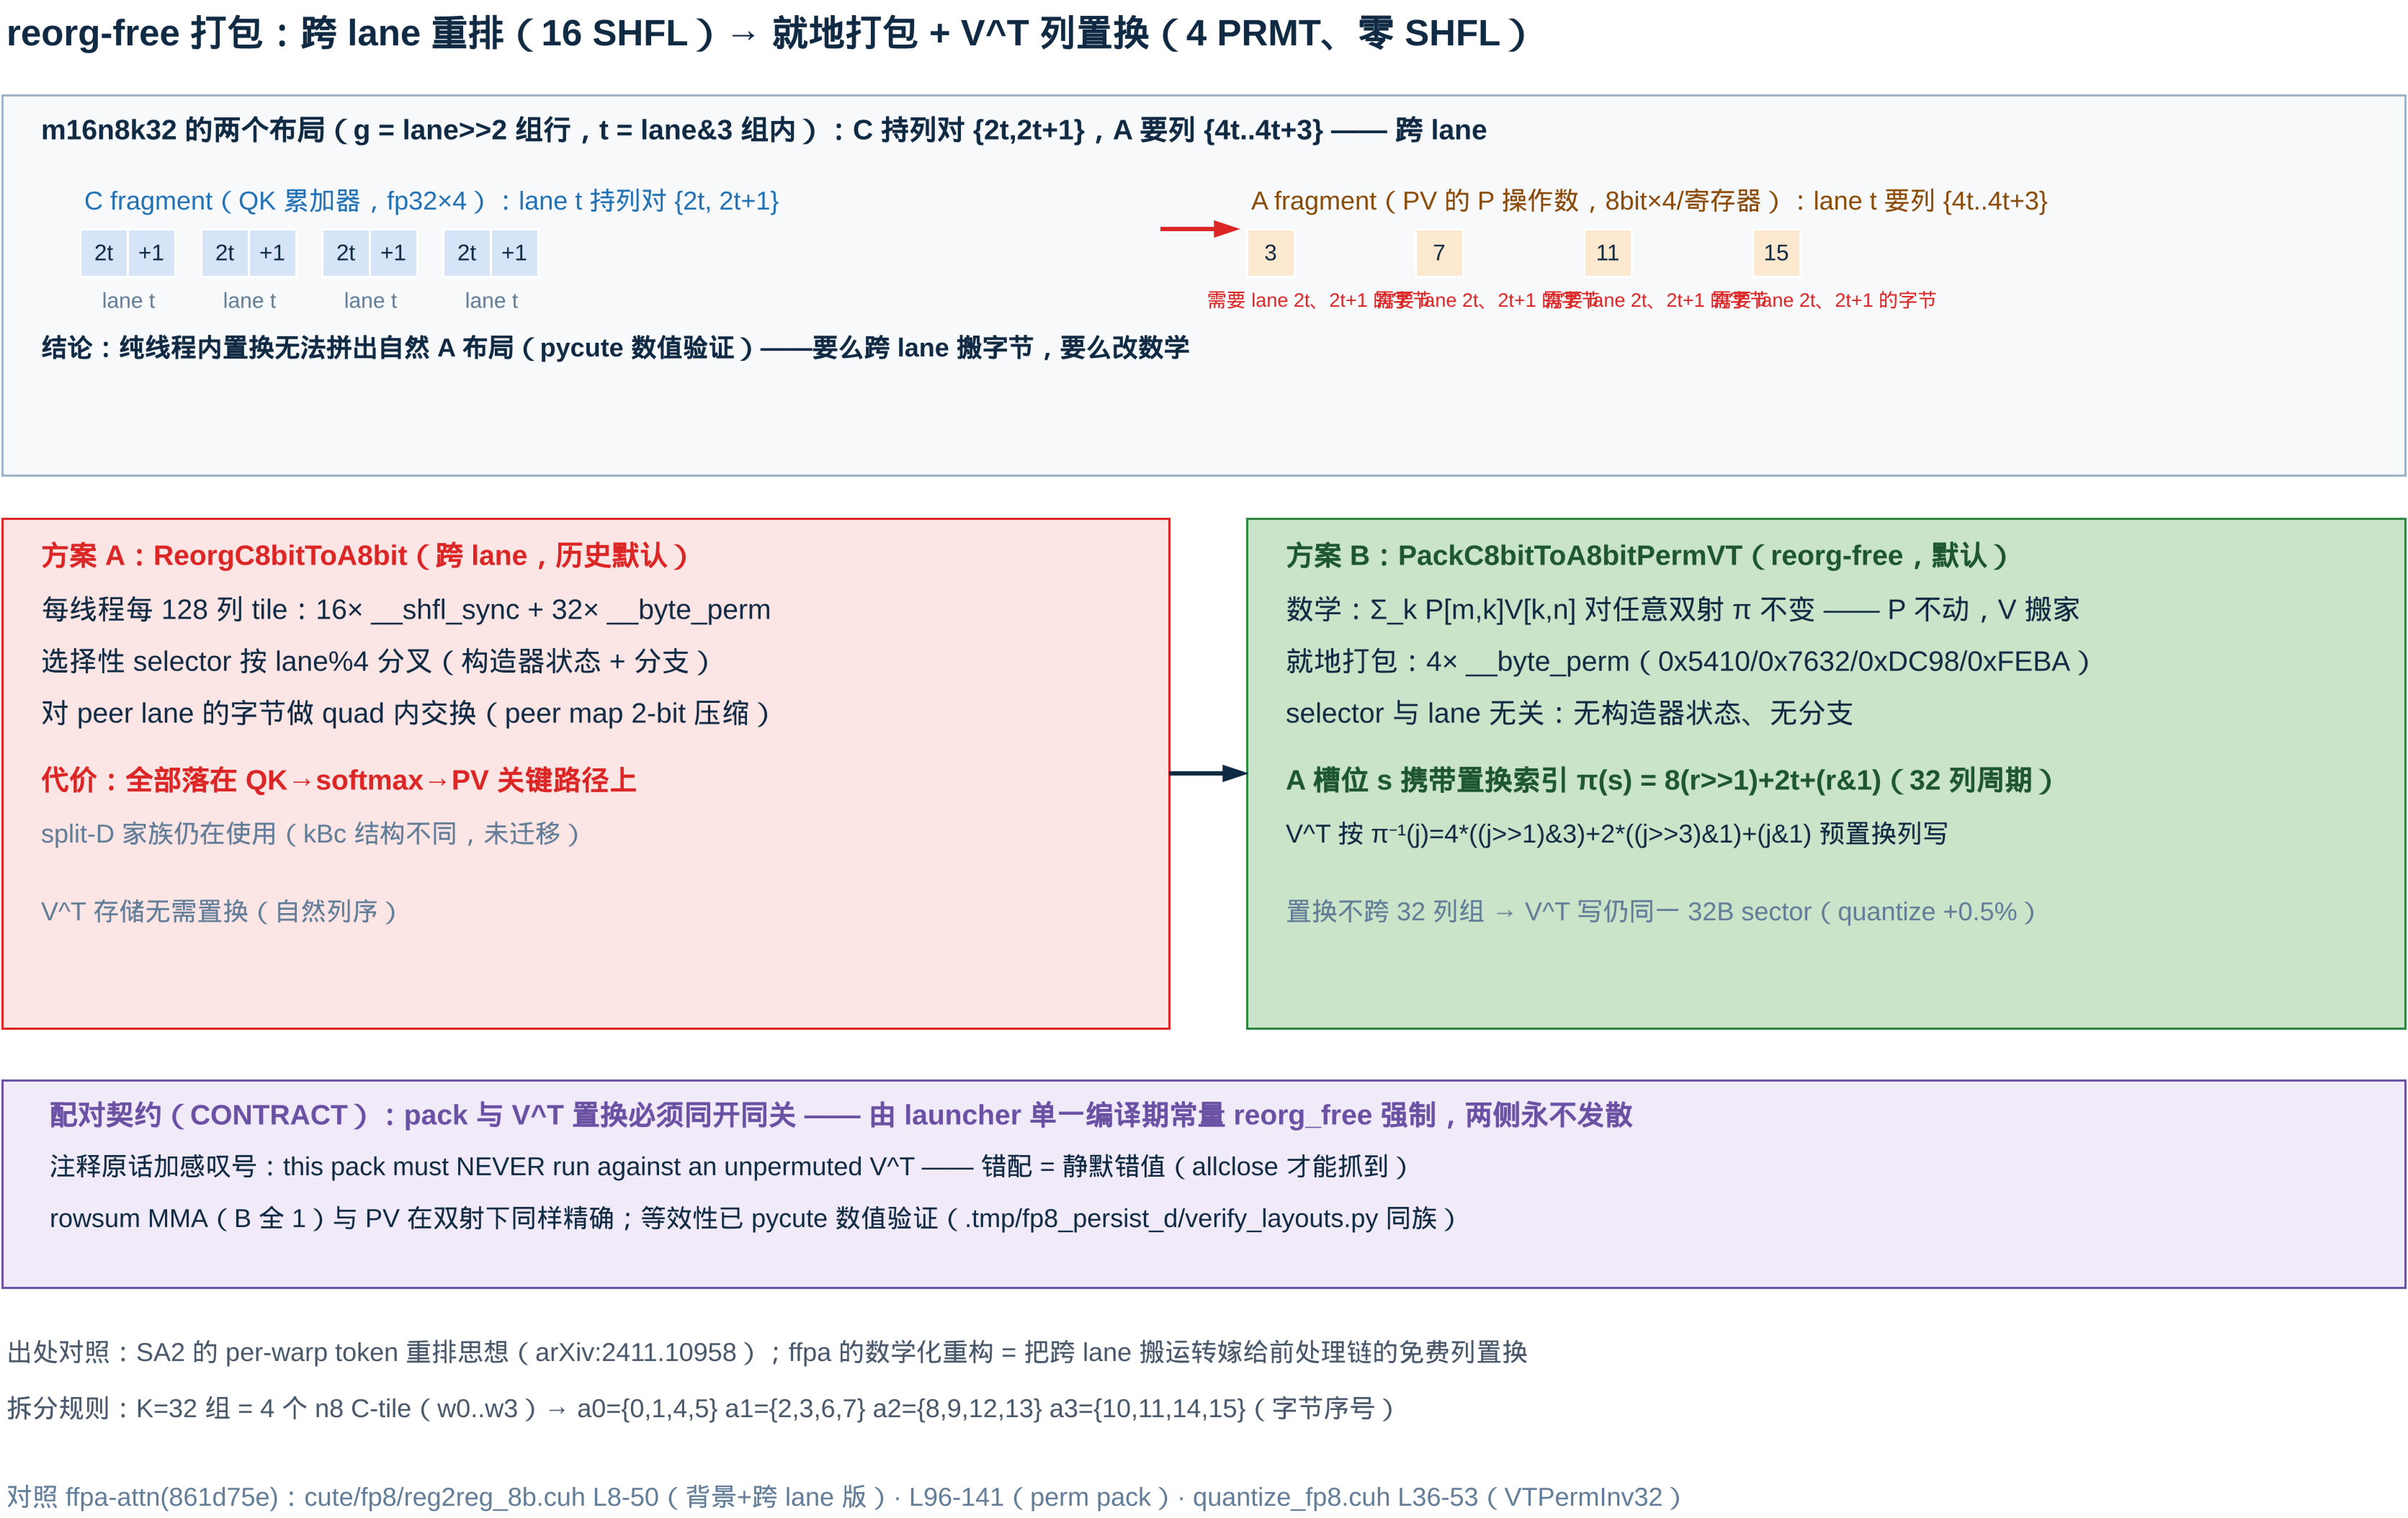
\includegraphics[width=0.98\textwidth]{figures/drawio/fig-29-3-reorg-free/fig-29-3-reorg-free.png}
  \begin{tikzpicture}
    \node[anchor=west, inner sep=0pt, align=left, font={\fontsize{7.4}{9.3}\selectfont \bfseries }] at (0.37,-0.354) {reorg-free 打包（每 128 列）：16 SHFL+32 PRMT $\to$ 16 PRMT、零 SHFL + V\^{}T 列置换};% w=17.125
    \node[draw=gray!55, fill=black!3, line width=0.5pt, minimum width=17.12cm, minimum height=2.71cm, inner sep=1pt, align=center, text width=17.06cm, font={\fontsize{5.7}{7.1}\selectfont }] at (8.932,-2.156) {};
    \node[anchor=west, inner sep=0pt, align=left, font={\fontsize{5.7}{7.1}\selectfont \bfseries }] at (0.616,-1.047) {m16n8k32 的两个布局（g = lane$>$$>$2 组行，t = lane\&3 组内）：C 持列对 {2t,2t+1}，A 要列 {4t..4t+3} ------ 跨 lane};% w=16.509
    \node[anchor=west, inner sep=0pt, align=left, font={\fontsize{5.2}{6.6}\selectfont \color{tkBlue} }] at (0.924,-1.555) {C fragment（QK 累加器，fp32$\times$4）：lane t 持列对 {2t, 2t+1}};% w=7.700
    \node[draw=none, fill=tkFillBlue, line width=0.5pt, minimum width=0.34cm, minimum height=0.34cm, inner sep=1pt, align=center, text width=0.28cm, font={\fontsize{4.6}{5.7}\selectfont }] at (1.093,-1.925) {2t};
    \node[draw=none, fill=tkFillBlue, line width=0.5pt, minimum width=0.34cm, minimum height=0.34cm, inner sep=1pt, align=center, text width=0.28cm, font={\fontsize{4.6}{5.7}\selectfont }] at (1.432,-1.925) {+1};
    \node[anchor=center, inner sep=0pt, align=center, font={\fontsize{4.4}{5.5}\selectfont \color{black!55} }] at (1.263,-2.264) {lane t};% w=0.678
    \node[draw=none, fill=tkFillBlue, line width=0.5pt, minimum width=0.34cm, minimum height=0.34cm, inner sep=1pt, align=center, text width=0.28cm, font={\fontsize{4.6}{5.7}\selectfont }] at (1.956,-1.925) {2t};
    \node[draw=none, fill=tkFillBlue, line width=0.5pt, minimum width=0.34cm, minimum height=0.34cm, inner sep=1pt, align=center, text width=0.28cm, font={\fontsize{4.6}{5.7}\selectfont }] at (2.295,-1.925) {+1};
    \node[anchor=center, inner sep=0pt, align=center, font={\fontsize{4.4}{5.5}\selectfont \color{black!55} }] at (2.125,-2.264) {lane t};% w=0.678
    \node[draw=none, fill=tkFillBlue, line width=0.5pt, minimum width=0.34cm, minimum height=0.34cm, inner sep=1pt, align=center, text width=0.28cm, font={\fontsize{4.6}{5.7}\selectfont }] at (2.818,-1.925) {2t};
    \node[draw=none, fill=tkFillBlue, line width=0.5pt, minimum width=0.34cm, minimum height=0.34cm, inner sep=1pt, align=center, text width=0.28cm, font={\fontsize{4.6}{5.7}\selectfont }] at (3.157,-1.925) {+1};
    \node[anchor=center, inner sep=0pt, align=center, font={\fontsize{4.4}{5.5}\selectfont \color{black!55} }] at (2.988,-2.264) {lane t};% w=0.678
    \node[draw=none, fill=tkFillBlue, line width=0.5pt, minimum width=0.34cm, minimum height=0.34cm, inner sep=1pt, align=center, text width=0.28cm, font={\fontsize{4.6}{5.7}\selectfont }] at (3.681,-1.925) {2t};
    \node[draw=none, fill=tkFillBlue, line width=0.5pt, minimum width=0.34cm, minimum height=0.34cm, inner sep=1pt, align=center, text width=0.28cm, font={\fontsize{4.6}{5.7}\selectfont }] at (4.019,-1.925) {+1};
    \node[anchor=center, inner sep=0pt, align=center, font={\fontsize{4.4}{5.5}\selectfont \color{black!55} }] at (3.85,-2.264) {lane t};% w=0.678
    \node[anchor=west, inner sep=0pt, align=left, font={\fontsize{5.2}{6.6}\selectfont \color{tkOrange!75!black} }] at (9.24,-1.555) {A fragment（PV 的 P 操作数，8bit$\times$4/寄存器）：lane t 要列 {4t..4t+3}};% w=7.700
    \node[draw=none, fill=tkFillOrange, line width=0.5pt, minimum width=1.00cm, minimum height=0.34cm, inner sep=1pt, align=center, text width=0.94cm, font={\fontsize{4.2}{5.2}\selectfont }] at (9.409,-1.925) {$(0\ldots3)$};
    \node[anchor=center, inner sep=0pt, align=center, font={\fontsize{3.9}{4.9}\selectfont \color{tkRed} }] at (9.748,-2.264) {需要 lane 2t、2t+1 的字节};% w=1.016
    \node[draw=none, fill=tkFillOrange, line width=0.5pt, minimum width=1.00cm, minimum height=0.34cm, inner sep=1pt, align=center, text width=0.94cm, font={\fontsize{4.2}{5.2}\selectfont }] at (10.611,-1.925) {$(4\ldots7)$};
    \node[anchor=center, inner sep=0pt, align=center, font={\fontsize{3.9}{4.9}\selectfont \color{tkRed} }] at (10.949,-2.541) {需要 lane 2t、2t+1 的字节};% w=1.016
    \node[draw=none, fill=tkFillOrange, line width=0.5pt, minimum width=1.00cm, minimum height=0.34cm, inner sep=1pt, align=center, text width=0.94cm, font={\fontsize{4.2}{5.2}\selectfont }] at (11.812,-1.925) {$(8\ldots11)$};
    \node[anchor=center, inner sep=0pt, align=center, font={\fontsize{3.9}{4.9}\selectfont \color{tkRed} }] at (12.151,-2.264) {需要 lane 2t、2t+1 的字节};% w=1.016
    \node[draw=none, fill=tkFillOrange, line width=0.5pt, minimum width=1.00cm, minimum height=0.34cm, inner sep=1pt, align=center, text width=0.94cm, font={\fontsize{4.2}{5.2}\selectfont }] at (13.013,-1.925) {$(12\ldots15)$};
    \node[anchor=center, inner sep=0pt, align=center, font={\fontsize{3.9}{4.9}\selectfont \color{tkRed} }] at (13.352,-2.541) {需要 lane 2t、2t+1 的字节};% w=1.016
    \node[anchor=west, inner sep=0pt, align=left, font={\fontsize{5.2}{6.6}\selectfont \bfseries }] at (0.616,-2.603) {结论：纯线程内置换无法拼出自然 A 布局（pycute 数值验证）------要么跨 lane 搬字节，要么改数学};% w=16.509
    \node[draw=tkRed, fill=tkFillRed, line width=0.5pt, minimum width=8.32cm, minimum height=3.63cm, inner sep=1pt, align=center, text width=8.25cm, font={\fontsize{5.7}{7.1}\selectfont }] at (4.528,-5.636) {};
    \node[anchor=west, inner sep=0pt, align=left, font={\fontsize{5.7}{7.1}\selectfont \bfseries \color{tkRed} }] at (0.616,-4.081) {方案 A：ReorgC8bitToA8bit（跨 lane，历史默认）};% w=7.823
    \node[anchor=west, inner sep=0pt, align=left, font={\fontsize{5.7}{7.1}\selectfont }] at (0.616,-4.466) {每线程每 128 列 tile：16$\times$ \_\_shfl\_sync + 32$\times$ \_\_byte\_perm};% w=7.823
    \node[anchor=west, inner sep=0pt, align=left, font={\fontsize{5.7}{7.1}\selectfont }] at (0.616,-4.836) {选择性 selector 按 lane\%4 分叉（构造器状态 + 分支）};% w=7.823
    \node[anchor=west, inner sep=0pt, align=left, font={\fontsize{5.7}{7.1}\selectfont }] at (0.616,-5.205) {对 peer lane 的字节做 quad 内交换（peer map 2-bit 压缩）};% w=7.823
    \node[anchor=west, inner sep=0pt, align=left, font={\fontsize{5.7}{7.1}\selectfont \bfseries \color{tkRed} }] at (0.616,-5.683) {代价：全部落在 QK$\to$softmax$\to$PV 关键路径上};% w=7.823
    \node[anchor=west, inner sep=0pt, align=left, font={\fontsize{5.2}{6.6}\selectfont \color{black!55} }] at (0.616,-6.068) {split-D 也可选此 fallback；reorg-free 同样受支持};% w=7.823
    \node[anchor=west, inner sep=0pt, align=left, font={\fontsize{5.2}{6.6}\selectfont \color{black!55} }] at (0.616,-6.622) {V\^{}T 存储无需置换（自然列序）};% w=7.823
    \node[draw=tkGreen, fill=tkFillGreen, line width=0.5pt, minimum width=8.25cm, minimum height=3.63cm, inner sep=1pt, align=center, text width=8.19cm, font={\fontsize{5.7}{7.1}\selectfont }] at (13.367,-5.636) {};
    \node[anchor=west, inner sep=0pt, align=left, font={\fontsize{5.7}{7.1}\selectfont \bfseries \color{tkGreen!70!black} }] at (9.486,-4.081) {方案 B：PackC8bitToA8bitPermVT（reorg-free，默认）};% w=7.762
    \node[anchor=west, inner sep=0pt, align=left, font={\fontsize{5.7}{7.1}\selectfont }] at (9.486,-4.466) {数学：$\Sigma$\_k P[m,k]V[k,n] 对任意双射 $\pi$ 不变 ------ P 不动，V 换列};% w=7.762
    \node[anchor=west, inner sep=0pt, align=left, font={\fontsize{5.7}{7.1}\selectfont }] at (9.486,-4.836) {每 K32 组 4$\times$ \_\_byte\_perm；128 列共 16 次};% w=7.762
    \node[anchor=west, inner sep=0pt, align=left, font={\fontsize{5.7}{7.1}\selectfont }] at (9.486,-5.205) {selector 与 lane 无关：无构造器状态、无分支};% w=7.762
    \node[anchor=west, inner sep=0pt, align=left, font={\fontsize{5.7}{7.1}\selectfont \bfseries \color{tkGreen!70!black} }] at (9.486,-5.683) {A 槽位：$\pi$(s)=8((s$>$$>$1)\&1)+2(s$>$$>$2)+(s\&1)（s$<$16）；$\pi$(s+16)=16+$\pi$(s)};% w=7.762
    \node[anchor=west, inner sep=0pt, align=left, font={\fontsize{5.2}{6.6}\selectfont }] at (9.486,-6.068) {V\^{}T 预置换：$\pi$$^{-1}$(j)=16*((j$>$$>$4)\&1)\\$+$4*((j$>$$>$1)\&3)+2*((j$>$$>$3)\&1)+(j\&1)};% w=7.762
    \node[anchor=west, inner sep=0pt, align=left, font={\fontsize{5.2}{6.6}\selectfont \color{black!55} }] at (9.486,-6.622) {置换不跨 32 列组 $\to$ V\^{}T 写仍同一 32B sector（quantize +0.5\%）};% w=7.762
    \node[draw=tkPurple, fill=tkFillPurple, line width=0.5pt, minimum width=17.12cm, minimum height=1.48cm, inner sep=1pt, align=center, text width=17.06cm, font={\fontsize{5.7}{7.1}\selectfont }] at (8.932,-8.562) {};
    \node[anchor=west, inner sep=0pt, align=left, font={\fontsize{5.7}{7.1}\selectfont \bfseries \color{tkPurple} }] at (0.678,-8.07) {匹配约定（CONTRACT）：pack 与 V\^{}T 置换必须同开同关 ------ 由 launcher 单一编译期常量 reorg\_free 强制，两侧永不发散};% w=16.509
    \node[anchor=west, inner sep=0pt, align=left, font={\fontsize{5.2}{6.6}\selectfont }] at (0.678,-8.439) {注释原话加感叹号：this pack must NEVER run against an unpermuted V\^{}T ------ 错配 = 静默错值（allclose 才能抓到）};% w=16.509
    \node[anchor=west, inner sep=0pt, align=left, font={\fontsize{5.2}{6.6}\selectfont }] at (0.678,-8.809) {rowsum MMA（B 全 1）与 PV 在双射下同样精确；等效性已 pycute 数值验证（.tmp/fp8\_persist\_d/verify\_layouts.py 同族）};% w=16.509
    \node[anchor=west, inner sep=0pt, align=left, font={\fontsize{5.2}{6.6}\selectfont \color{black!65} }] at (0.37,-9.764) {出处对照：SA2 的 per-warp token 重排思想（arXiv:2411.10958）；ffpa 的数学化重构 = 把跨 lane 搬运转嫁给前处理链的顺带列置换};% w=17.125
    \node[anchor=west, inner sep=0pt, align=left, font={\fontsize{5.2}{6.6}\selectfont \color{black!65} }] at (0.37,-10.164) {拆分规则：K=32 组 = 4 个 n8 C-tile（w0..w3）$\to$ a0={0,1,4,5} a1={2,3,6,7} a2={8,9,12,13} a3={10,11,14,15}（字节序号）};% w=17.125
    \node[anchor=west, inner sep=0pt, align=left, font={\fontsize{5.2}{6.6}\selectfont \color{black!55} }] at (0.37,-10.795) {对照 ffpa-attn(861d75e)：cute/fp8/reg2reg\_8b.cuh L8-50（背景+跨 lane 版）$\cdot$ L96-141（perm pack）$\cdot$ quantize\_fp8.cuh L36-53（VTPermInv32）};% w=17.125
    \draw[tkRed, line width=0.8pt, -{Stealth[length=2.2pt,width=1.8pt]}] (8.624,-1.756) -- (9.178,-1.756);
    \draw[black!75, line width=0.8pt, -{Stealth[length=2.2pt,width=1.8pt]}] (8.686,-5.636) -- (9.24,-5.636);
  \end{tikzpicture}
  \caption{reorg-free 打包对照（每线程每 128 列）：跨 lane 重排
  16 SHFL + 32 PRMT vs 就地打包 16 PRMT、零 SHFL + $V^{\top}$ 列置换；
  每个 $K{=}32$ 组为 4 PRMT。归约轴双射不变性保证精确等价。}
  \label{fig:29-reorg-free}
\end{figure}

\section{性能分析}

\subsection{本机实测（RTX PRO 5000，B1 H32 N8192，bench 默认配置）}

\begin{center}
\begin{tabular}{llcccc}
\toprule
$D$ & task & FFPA & SDPA & TFLOPS & speedup \\
\midrule
64  & self-attn & 1.91ms & 2.40ms & 288T & 1.26$\times$ \\
64  & causal    & 1.16ms & 1.34ms & 237T & 1.16$\times$ \\
128 & self-attn & 3.02ms & 5.12ms & 365T & \textbf{1.70$\times$} \\
128 & causal    & 1.85ms & 2.68ms & 297T & 1.45$\times$ \\
192 & self-attn & 4.58ms & 7.27ms & 360T & 1.59$\times$$^{*}$ \\
\bottomrule
\end{tabular}
\end{center}
$^{*}$D=192 存在正确性 bug（29.7.1~节），速度数据仅供参考。D=64 的收益
小于 D=128 是因为 attention 的算术强度随 $D$ 下降、quantize aux 链占比
上升。kernel 级与 SageAttention 对比稳定 $+1.1\sim2.3\%$（仓库 nsys
per-kernel 记录）。

\subsection{微优化上限：证伪清单}

persist-D 的结构优化路线已被系统实测证伪（完整清单见仓库 RFC
\S5.8）：WS 双 consumer（FA3 式 2$\times$128T）负优化；persistent work
loop 零收益（tensor-bound 77\%）；stages 加深负（K2V2 预取已领先）。
v2/v3/v5（128P+128C、无 WS、V 驻留寄存器）分别 $+31.6\%$/$+1.4\%$/$+48\%$
（追平基线的是 v3 加 v\_full wait hoist，即 v4，$-0.1\%$）；
cluster 化无 DSMEM 需求、持平或更慢；CUDA-core row-sum 替代 tensor
rowsum MMA $-4\%$。已落地的优化（D=128）：rescale+absorb FFMA
融合、max-pass 延迟 scale、per-row rescale gating、Q quant 2 线程/行。
负结果把后续优化方向的搜索空间压缩到了 engine 层（aux 链 overlap）。

\subsection{带宽与算术的边界}

D=128、N=8192 时主 kernel 365T FLOPS 对应的 DRAM 流量很小（$O(N\cdot D)$
量级 workspace 单遍），瓶颈在 tensor pipe 与 softmax 的依赖链，与
fp16 家族同构；但 fp8 的 MMA 吞吐翻倍使 softmax/P 打包的相对占比上升，
这也是 \texttt{kMaxScaleAfter}、FFMA 吸收融合这类\textbf{指令级}优化
在此路径收益显著的原因。

\section{实践经验}

\subsection{案例：D=192 正确性 bug 的定位（定位实录）}\label{sec:29-d192}

写本章的 bench 验证时发现 \texttt{--cuda-impl fp8 --D 192}
allclose 失败（fp16/bf16 双双 $\times$），而 D=64/128 全绿。定位过程
记在这里，可作为同类问题的排查参考。

后续状态：该 bug 已由上游 \texttt{\#382} 修复（Q tile 区与 K stage 的 smem 复用
竞态，影响整个 $D>128$ 窗口，即 $D{=}160/192/224$），\texttt{\#385} 随后撤销了
警告，0.2.5 起不再复现。本节保留 861d75e 上的定位过程；下面\textbf{配置矩阵消去}
停在三选一嫌疑，已确证的根因是复用竞态，不是 $D{=}192$ 特有。
\begin{enumerate}[itemsep=1pt,topsep=2pt]
  \item \textbf{误差量级分类}：max\_abs=2.66 vs mean\_abs=0.011。均值是
        正常 fp8 精度，最大值远超正常量化误差 $\Rightarrow$ \textbf{正确性 bug}
        （个别行错），不是精度不足；
  \item \textbf{行模式定位}：per-row max 直方图显示坏行集中在
        $row\bmod128\in[64,127]$（每个 128 行 Q tile 的后半）；
  \item \textbf{N 缩放}：N=512 时几乎全错、N=8192 时只剩 11\% 行错，
        错误随 N 稀释，说明错的是\textbf{特定 (row, kv-tile) 组合}而非
        系统性索引错位；
  \item \textbf{配置矩阵消去}：默认/纯 fp8 f32acc/int8+f16acc/no-smK/
        per-thread/per-channel 全部 $\times$ $\Rightarrow$ 与量化 knob 无关，
        bug 在 D=192 特有的主 kernel 路径（$kBc{=}64$ 变体、SW64 swizzle、
        或 quantize 侧 kBlockRows 与 kBc 的一致性）；
  \item \textbf{fp16 对照}：fp16 CUTE 路径 D=192 完全正确
        （max=0.0001）$\Rightarrow$ 输入布局、TMA 与寻址层没有问题，问题范围缩小到
        fp8 专属代码。
\end{enumerate}

\begin{figure}[H]
\centering
\begin{tikzpicture}[font=\scriptsize]
  \definecolor{alertred}{RGB}{178,34,34}
  \def\gw{0.86}
  \def\gh{0.33}
  \foreach \rb in {0,...,15}{
    \foreach \c in {0,...,2}{
      \ifnum\rb<8
        \pgfmathtruncatemacro{\gr}{int(16+14*\c)}
        \fill[gray!\gr] ({\c*\gw},{-(\rb+1)*\gh}) rectangle ({(\c+1)*\gw},{-\rb*\gh});
      \else
        \fill[alertred!45] ({\c*\gw},{-(\rb+1)*\gh}) rectangle ({(\c+1)*\gw},{-\rb*\gh});
      \fi
    }
  }
  \draw[thin] (0,0) grid[xstep=0.86cm, ystep=0.33cm] ({3*\gw},{-16*\gh});
  \draw[very thick] (0,0) rectangle ({3*\gw},{-16*\gh});
  \draw[alertred, very thick, dashed] (-0.10,{-8*\gh}) -- ({3*\gw+0.10},{-8*\gh});
  \node[anchor=south] at ({0.5*\gw},0.06) {0--63};
  \node[anchor=south] at ({1.5*\gw},0.06) {64--127};
  \node[anchor=south] at ({2.5*\gw},0.06) {128--191};
  \node[anchor=south, font=\scriptsize\bfseries] at ({1.5*\gw},0.60) {O 列（$D{=}192=3\times64$ 拼接视图）};
  \node[anchor=south] at ({1.5*\gw},0.34) {persist-D，$k_{Bc}{=}64$ 变体};
  \foreach \rb/\rl in {0/0,4/32,8/64,12/96,16/128}{
    \node[anchor=east, font=\tiny] at (-0.08,{-\rb*\gh}) {\rl};
  }
  \node[anchor=east, font=\tiny, rotate=90] at (-0.52,{-8*\gh}) {row mod 128};
  \node[alertred, font=\tiny, anchor=west] at ({3*\gw+0.16},{-8*\gh}) {64};
  \node[anchor=west, align=left, text width=8.6cm] at ({3*\gw+0.85},-0.35)
    {$\bullet$~\textbf{坏行区}：row mod 128 $\in[64,127]$——每个 128 行 Q tile
     的后半（红色带，每带 = 8 行）；正常行灰度按 D chunk 区分。};
  \node[anchor=west, align=left, text width=8.6cm] at ({3*\gw+0.85},-1.85)
    {$\bullet$~\textbf{N 稀释}：N=512 几乎全错 $\to$ N=8192 仅 11\% 行错
     ——错误随 N 稀释，说明是特定 (row, kv-tile) 组合而非系统性索引错位。};
  \node[anchor=west, align=left, text width=8.6cm] at ({3*\gw+0.85},-3.35)
    {$\bullet$~\textbf{max/mean 分裂}：max\_abs=2.66 vs mean\_abs=0.011
     ——个别行严重错误 + 正常均值 $\Rightarrow$ 正确性 bug，非精度不足。};
  \node[anchor=west, align=left, text width=8.6cm] at ({3*\gw+0.85},-4.85)
    {$\bullet$~\textbf{嫌疑范围}（fp16 对照路径已排除）：$k_{Bc}{=}64$ 变体 /
     SW64 swizzle / 量化侧 kBlockRows 一致性。};
\end{tikzpicture}
\caption{D=192 正确性 bug 的坏行定位（29.7.1~节五步法的可视化）：把 $O$ 视为
3$\times$64 列拼接，坏行集中在 row mod 128 $\in[64,127]$（每个 128 行 Q tile 的
后半）；N=512 几乎全错而 N=8192 仅 11\% 行错（N 稀释 $\Rightarrow$ 特定
(row, kv-tile) 组合）；max\_abs=2.66 对 mean\_abs=0.011 的分裂说明错误集中在个别行。}
\label{fig:29-d192-rows}
\end{figure}

教训：速度好、均值好都不等于正确。bench 的 allclose 是唯一
硬门槛；误差的 max/mean 分裂是个别行错的强信号；行号模 tile 尺寸的
直方图能直接把 bug 锚到 tile 结构的哪一半。

\subsection{考据：sm\_89 的 cp.async 变体}

同文件名在 \texttt{cute/fp8/sm\_89/persist\_d.cuh} 有一个 Ada 变体：
无 TMA/mbarrier，用 sm80 装载协议（cp.async + \texttt{wait<2S-1>}）复用
sm120 的计算层（int8 QK / fixed p\_scale / f8f8f16 PV），256T non-WS。
其 NCU 结论（依赖链/发射受限，\texttt{math\_pipe\_throttle} 1.32 $\gg$
\texttt{wait} 0.82）与深流水零收益的证伪记录，正好构成同一算法在不同
装载协议下瓶颈迁移的对照。本节不展开，读者按需查阅仓库优化 RFC
（PC-16、附录 \#22）。

\section{常见坑}

\begin{enumerate}[itemsep=1pt,topsep=2pt]
  \item \textbf{P 是 online 量化，无法离线校准}：Q/K/V 都能离线 smoothing
        /per-channel 校准，P 每 tile 现算现量化，值域与分布逐行剧变
        （causal 早行近 one-hot、dense 行近均匀），只能选固定/保守发射域。
        这是量化 attention 精度损失的主要根源之一（实测 P 0.11 与 QK 0.13
        同量级、V 0.19 最大）。
  \item \textbf{满量程发射与 lazy rescale 互斥}：per-channel V 的发射
        $P\cdot448$ 铺满量程，stale max
        的 $2^T$ 膨胀必然 satfinite（29.3.3~节）；fp8 traits 直接关掉
        lazy rescale，且 f16 acc 路径把 rescale 融进吸收 FFMA 后延迟惩罚
        消失。
  \item \textbf{kVTPerm 的匹配是编译期规则}：\texttt{PackC8bitToA8bitPermVT}
        对未置换的 $V^{\top}$ 运行 = 静默错值。匹配由 launcher 单一常量
        强制；绕过 launcher 直接调 kernel 没有保护。
  \item \textbf{f16 PV 累加域}：$kBc\cdot448\cdot2.25\le65504$ 的编译期
        检查不过时 P 域自动收到 224。不理解这条约束，会以为 P 域有时
        448 有时 224 是随机行为。
  \item \textbf{early rows 的 ESS 幅度放大}（27.3.7~节）：causal 前几行
        ESS$\approx$1、幅度 $3.1\sigma$，fp8 每级 $\sim$5\% 相对误差换算
        成 15$\times$ 于 dense 的绝对误差；早行 fp16 QK 不能消除主导误差
        （V 量化是最大单项）。可选 hybrid 全链 fp16；若保留量化路径，
        则用 per-channel V scale 压 V 的相对误差（第~\ref{ch:28}~章）。
  \item \textbf{D=192（$kBc{=}64$ 变体）在 861d75e（$\le$0.2.4）上有正确性 bug}：
        Q tile 区与 K stage 的 smem 复用竞态，影响 $D>128$ 的整个窗口；
        0.2.5 起已修（上游 \texttt{\#382}/\texttt{\#385}），29.7.1~节记录的是旧版本现象。
\end{enumerate}

\section{面试要点速查}

\begin{enumerate}[itemsep=1pt,topsep=2pt]
  \item fp8 attention 的所有 scale 是如何消去的？
        （$\delta_Q\delta_K$ 折 exp2 系数；$v_s$ 折 P 发射域，在未舍入代数中消去；
        $p_{scale}$ 收 epilogue——式~\ref{eq:29-sdequant}--\ref{eq:29-threestep}。）
  \item 为什么 P 的量化只能 fixed/保守，不能离线校准？
        （P 每 tile 现算、分布逐行剧变；离线对象必须前向开始前存在。）
  \item lazy rescale 与满量程 P 为什么互斥？（$2^T$ 膨胀 vs 448 satfinite，
        29.3.3~节；f16 acc 路径 FFMA 吸收让 rescale 免费。）
  \item f16 PV 累加器的域怎么算？（ffpa 跨 $kBc$ 整 tile 累加：
        $kBc\cdot P_r\cdot V_r\le65504$，$V_r=2.25$ 时 $kBc{\le}64$ 装
        P 448、$kBc{=}128$ 收到 224；SA2++ 单指令口径 $65504/32=2047$、
        双侧收窄 $224\times4.5$。）
  \item reorg-free 打包省了什么、代价是什么？（每 128 列：16 SHFL+32 PRMT $\to$
        16 PRMT 零 SHFL；代价 $V^{\top}$ 列置换预写 + 编译期匹配规则，
        式~\ref{eq:29-perm-inv}。）
  \item Q 的 s2r 常驻为什么省钱？省的是 occupancy 吗？
        （不是。省 smem（16KB Q 区复用）$\to$ 买 L1 共池容量，
        $\sim$4--5$\mu s$/16KB；CTA 驻留本就寄存器受限。）
  \item fp8 persist-D 的 D 范围与家族分工？（$\le$224 %32；更大走
        split-D M8N1 / M4N2，第~\ref{ch:30}~章。）
\end{enumerate}

\section{最小测试与动手实验}

\begin{lstlisting}[style=console]
# 环境（Card 7，小 headdim 放行）
$ conda activate cdit
$ export CUDA_VISIBLE_DEVICES=7 FFPA_CUDA_ALLOW_SMALL_D=1

# [A] persist-D 域内全绿组合：D=64 / 128
$ python -m ffpa_attn.bench --fwd-backend cuda --cuda-impl fp8 \
    --tasks self-attn,causal --D 128 --no-bwd --show-allclose
# self-attn fp16  8192/8192  3.02ms  365T  1.70x  allclose OK
# causal    fp16  8192/8192  1.85ms  297T  1.45x  allclose OK

# [B] 配置显式声明（int8 QK + f16 PV acc）
$ python -m ffpa_attn.bench --fwd-backend cuda --cuda-impl fp8 \
    --tasks self-attn --D 128 --no-bwd --show-allclose \
    --fp8-qk-mm-type int8 --fp8-pv-acc-type f16
# 3.08ms  357T  1.67x  allclose OK

# [C] D=192：正确性 bug 复现（29.7.1 节）
$ python -m ffpa_attn.bench --fwd-backend cuda --cuda-impl fp8 \
    --tasks self-attn --D 192 --no-bwd --show-allclose
# allclose FAIL  ← 坏行集中在 row%128 ∈ [64,127]
\end{lstlisting}

\textbf{实验 1（scale 流向追踪）}：把 \texttt{persist\_d.cuh} 的
Phase 1--5 各自在纸上标出哪个 scale 在哪条指令上被乘或被消去，对照
图~\ref{fig:29-scale-folding}，练到能默写三步协议。
\textbf{实验 2（发射域 A/B）}：\texttt{FFPA\_FP8\_PQUANT\_PER\_ROW=1}
重跑 [A]，观察精度提升与速度代价（per-row 归约 + $o\_tile$ 暂存）。
\textbf{实验 3（bug 定位复演）}：按 29.7.1~节步骤用 PyTorch 复现 D=192
的行模式直方图（脚本思路：per-row max diff $>$ 0.1 统计
$row\bmod128$），把速度好、均值好不等于正确这条固化成检查习惯。
\textbf{实验 4（lazy rescale 证伪）}：读 \texttt{attn\_traits.cuh}
L31--37 注释，回答为什么 fp8 关掉 lazy rescale 而 fp16 开着。

\section*{延伸阅读}
\begin{itemize}[itemsep=0pt,topsep=2pt]
  \item SageAttention2（arXiv:2411.10958）：per-warp token 重排与 int8 QK
        的原始出处（reorg-free 打包的对照原型）。
  \item SageAttention2++（arXiv:2505.21136）\S3.1：f16 PV 累加域约束
        （$P_r\times V_r\le2047$）的推导。
  \item FlashAttention-4（arXiv:2603.05451）：lazy rescale 与量化域交互
        （本章 29.3.3~节的反例来源）。
  \item ffpa-attn \texttt{reg2reg\_8b.cuh} 头注释：C$\to$A fragment
        布局的 PTX 级推导与 pycute 数值验证记录。
  \item ffpa-attn 仓库 RFC \S5.8：persist-D 结构优化的完整证伪清单。
\end{itemize}

% ch30-fp8-split-d-m4n2.tex — FP8(三)：split-D 与 M4N2——大 D 的两个瓶颈（RFC-K4）
% 源码：ffpa-attn(861d75e) cute/fp8/sm_120/split_d.cuh(956L) + split_d_m4n2.cuh(989L)
%       + attn_traits.cuh(L109-311) + softmax.cuh(L74-231) + dispatch/cute_fp8.cuh
\chapter{FP8（三）：split-D 与 M4N2——大 $D$ 的两个瓶颈}\label{ch:30}

\section{本章导读}

第~\ref{ch:29}~章的 persist-D 把整个 $K$ tile（$B_c\times D$）一次装进
smem、让单个 warp 独占 $O$ 的全部 $D$ 列。这在 $D\le 224$ 时是最优解；
但 $D$ 继续增大，会同时遇到两个瓶颈：

\begin{enumerate}[itemsep=0pt,topsep=2pt]
  \item \textbf{smem 瓶颈}：$K$ tile 字节数 $O(D)$，99KB 预算装不下，
        由 \textbf{split-D}（D 维分块）解决；
  \item \textbf{寄存器瓶颈}：$O$ 累加器 $O(D)$ 个 f32 寄存器/线程，逼近
        255 上限，由 \textbf{M4N2 TiledMMA}（atom 布局重排）解决。
\end{enumerate}

两个瓶颈正交：只做 split-D，寄存器照旧 $O(D)$；只做 M4N2，smem 照旧装不下。
ffpa-attn 的 dispatch 按 $D$ 三分（\texttt{dispatch/\allowbreak{}cute\_fp8.cuh}
L60--64）：

\begin{center}
\begin{tabular}{@{}llll@{}}
\toprule
$D$ 范围 & kernel & atom 布局 & $O$ 寄存器/线程 \\
\midrule
$D\le 224$ & \texttt{persist\_d}（第~\ref{ch:29}~章） & M8N1 & $D/2$ \\
$224<D<768$ & \texttt{split\_d.cuh}（本章） & M8N1 & $D/2$ \\
$D\ge 768$ & \texttt{split\_d\_m4n2.cuh}（本章） & M4N2 & $D/4$ \\
\bottomrule
\end{tabular}
\end{center}

本章先推导 split-D 的分块恒等式（为什么它是精确变换，一个比特
都不差），再建立 M4N2 的寄存器压力模型（为什么 $N$ 维划分能压低每线程
累加器、而每 SM 的总量只由 $M_w$ 决定），最后走读两个 kernel 的实现差异，
特别是 M4N2 带来的多项新代价：
P 的 SMEM roundtrip、跨 N-warp softmax 归约、$k_{Br}$ 减半与量化块
错位等。所有机制均以
fp8 家族为主线；fp16 家族同构（第~\ref{ch:25}~章已见其 fp16 版），fp4
家族见第~\ref{ch:32}~章。

\section{问题与动机}

\subsection{两个瓶颈的数量级}

smem 瓶颈容易估算：fp8 下 1B/元素，$B_c=128$ 的 $K$ tile 在 $D=512$ 时是
64KB，加上 V stage 与 Q 就超 99KB 预算。persist-D 把 Q 区的槽位 0 复用给
最后一个 K stage，才能在 $D\le 224$ 时装下；$D$ 再大，唯一的办法是把 $D$ 切块流水。

寄存器瓶颈隐蔽一些。m16n8k32 atom 的 C-fragment 每 thread 持 4 个 f32；
M8N1 布局（8 个 M-warp、N 维单 warp 满编）让单 warp 独占输出的完整 $D$
列。$k_{Br}=128$ 时 $O$ 累加器寄存器数是
\begin{equation}\label{eq:30-oacc-m8n1}
O_{\text{acc}}=\frac{k_{Br}\cdot D}{256\ \text{threads}}=\frac{D}{2}
\quad(\text{f32 regs/thread},\ k_{Br}=128),
\end{equation}
$D=512$ 时 256 个寄存器超上限 1 个（255），属边缘 spill；
$D\ge 896$ 大量 spill，性能急剧下降。实测（5090，fp16 家族同构）：$D=1024$ 时 M8N1 的
$O_{\text{acc}}=512$ regs 溢出到 local memory，吞吐掉到 $\sim$100T；
而 M4N2 同 $D$ 边缘 spill 仍有 154T。

\subsection{split-D 与 M4N2 各解决一个瓶颈}

split-D 回答 smem 怎么装下：把 $D$ 切成 $D/k_{VDChunk}$ 个
chunk，K/V 的 TMA 与 MMA 都按 chunk 流水，smem 只需常驻
$(k_{Br}+k_{Bc})\times k_{QKDChunk}+k_{Bc}\times k_{VDChunk}$ 每 stage，
与总 $D$ 无关。M4N2 回答寄存器怎么装下：把 atom 布局从
$(8,1,1)$ 换成 $(4,2,1)$（4 个 M-warp 乘 2 个 N-warp），让每
thread 的 $O$ 列持有量减半（\ref{sec:30-regmodel}~节的推导）。

代价各自独立：split-D 多了每 chunk 一次 producer-consumer 握手；M4N2
使 $k_{Br}$ 从 128 减到 64（CTA 数翻倍）、P 必须走 SMEM roundtrip、
softmax 需要跨 N-warp 归约。交叉点在 $D=768$：之下 M8N1 更快（无
roundtrip 开销、$k_{Br}$ 大一倍），之上 M4N2 的寄存器收益开始占优
（30.6.2~节）。

\subsection{causal 精度的已知边界}

\texttt{split\_d.cuh} 的头注释（L40--43）声明了 causal 精度边界：
逐元素误差上界（causal 早期行 attend 的 key 少，
QK/P 量化误差无法被平均）：
$O$ 误差可保持在 $10^{-1}$ 量级但 lse 误差可达 $\sim 6\times10^{-2}$
（近 1 概率的 e4m3 舍入），dense 则 $\sim 4\times10^{-3}$（m4n2 头注释无相同
声明，但精度结构相同）。本机实测
（30.6~节）三个 $D$ 的 causal 误差模式完全一致：序列前
$\sim$30\% 的行误差大、其余干净、dense 全绿，这是 fp8 路径的
\textbf{已知特性}而非 bug，工程解法是 hybrid（前若干行走 fp16
stage-1，\texttt{dispatch/cute\_fp8.cuh} L55--58 的 FC-3 注释），
不在本章展开。

\section{数学原理}

\subsection{split-D 分块恒等式：精确，不是近似}\label{sec:30-identity}

设 $D=\mathcal{D}_0\cup\mathcal{D}_1\cup\cdots$ 按 chunk 划分。QK 侧
$D$ 是\textbf{归约维}：
\begin{equation}\label{eq:30-qk-split}
S=QK^{\top}=\sum_{c}Q_{:,\mathcal{D}_c}\,K^{\top}_{:,\mathcal{D}_c},
\end{equation}
每个 chunk 一次 MMA 累加进同一个 $S$ fragment。fp8 路径 f32
累加；int8 路径 s32 累加（精确，$\ll 2^{31}$）后一次性 cast（L495--503），
split 不引入任何新的舍入点。PV 侧 $D$ 是\textbf{输出列维}。用原始 $V(N,D)$ 写：
\begin{equation}\label{eq:30-pv-split}
O_{:,\mathcal{D}_c}=P\,V_{:,\mathcal{D}_c}
 =P\bigl(V^{\top}_{\mathcal{D}_c,:}\bigr)^{\top},
\end{equation}
各 chunk 的 $O$ 段\textbf{独立累加}，互不干扰。

关键观察：softmax 的行统计（$m_r$、$\ell_r$）是\textbf{KV 行维的量}，
与 $D$ 的切分完全无关：split-D 不产生每 chunk 各自的
row max/row sum，所有 chunk 共享同一组 $(m,\ell)$，rescale 因子天然
一致。这就是 \texttt{split\_d.cuh} 的结构（L440--443 注释）：QK chunk
循环在 softmax 之前全部完成（L446--483），softmax 之后 V
chunk 循环各自把 $P V_{:,\mathcal{D}_c}$ 加进
\texttt{o\_acc\_storage[c]}（L678--756）。

\begin{figure}[H]
\centering
\begin{tikzpicture}[font=\scriptsize, >=Stealth]
  \node[anchor=south, font=\scriptsize\bfseries] at (6.6,0.62)
    {split-D 分块恒等式：QK 归约维累加，PV 输出列维独立};
  \node[anchor=south, font=\tiny] at (6.6,0.38)
    {示例 $D{=}128$（$k_{VDChunk}{=}64\Rightarrow 2$ 个 chunk；通用 $D/k_{VDChunk}$ 个）};
  \draw[fill=gray!18] (0,-0.75) rectangle (1.5,-0.15);
  \draw[fill=gray!55] (0,-1.55) rectangle (1.5,-0.95);
  \draw[tkBlue, thick] (0,-0.75) rectangle (1.5,-0.15);
  \draw[tkBlue, thick] (0,-1.55) rectangle (1.5,-0.95);
  \node at (0.75,-0.45) {$Q_{:,\mathcal{D}_0}$};
  \node at (0.75,-1.25) {$Q_{:,\mathcal{D}_1}$};
  \node[anchor=east, font=\tiny] at (-0.12,-0.45) {$Q$};
  \node[anchor=east, font=\tiny] at (-0.12,-1.25) {（$M{\times}D$）};
  \draw[fill=gray!18] (0,-2.45) rectangle (1.5,-1.85);
  \draw[fill=gray!55] (0,-3.25) rectangle (1.5,-2.65);
  \draw[tkBlue, thick] (0,-2.45) rectangle (1.5,-1.85);
  \draw[tkBlue, thick] (0,-3.25) rectangle (1.5,-2.65);
  \node at (0.75,-2.15) {$K^{\top}_{\mathcal{D}_0,:}$};
  \node at (0.75,-3.0) {$K^{\top}_{\mathcal{D}_1,:}$};
  \node[anchor=east, font=\tiny] at (-0.12,-2.15) {$K^{\top}$};
  \node[anchor=east, font=\tiny] at (-0.12,-3.0) {（$D{\times}B_c$）};
  \draw[->, tkBlue] (1.55,-0.45) -- (2.42,-0.82);
  \draw[->, tkBlue] (1.55,-2.15) -- (2.42,-1.08);
  \draw[->, tkBlue] (1.55,-1.25) -- (2.42,-2.38);
  \draw[->, tkBlue] (1.55,-3.0) -- (2.42,-2.62);
  \draw[tkBlue, thick] (2.5,-0.95) circle (0.40);
  \node at (2.5,-0.95) {\tiny MMA};
  \draw[tkBlue, thick] (2.5,-2.55) circle (0.40);
  \node at (2.5,-2.55) {\tiny MMA};
  \draw[->, tkBlue] (2.9,-1.15) -- (3.28,-1.48);
  \draw[->, tkBlue] (2.9,-2.35) -- (3.28,-2.02);
  \draw[tkBlue, thick] (3.62,-1.75) circle (0.34);
  \node at (3.62,-1.75) {$\Sigma_c$};
  \draw[->, tkBlue] (3.96,-1.75) -- (4.45,-1.75);
  \draw[tkBlue, fill=white, thick] (4.5,-2.4) rectangle (6.0,-1.1);
  \node at (5.25,-1.62) {$S$ fragment};
  \node at (5.25,-2.12) {\tiny 同一 C 累加器};
  \node[anchor=south, font=\tiny, align=center] at (5.25,-1.02)
    {归约维：chunk 累加\\（式~\ref{eq:30-qk-split}，无新舍入点）};
  \draw[->, tkOrange] (6.05,-1.75) -- (6.55,-1.75);
  \node[above, font=\tiny, text=tkOrange] at (6.3,-1.68) {$P$};
  \draw[tkOrange, fill=white, thick] (6.6,-2.3) rectangle (8.0,-1.2);
  \node at (7.3,-1.62) {softmax};
  \node at (7.3,-2.10) {\tiny 全 $D$ 一次};
  \draw[->, tkOrange] (8.05,-1.6) -- (8.55,-1.08);
  \draw[->, tkOrange] (8.05,-1.9) -- (8.55,-2.42);
  \draw[tkOrange, thick] (8.95,-0.95) circle (0.40);
  \node at (8.95,-0.95) {\tiny MMA};
  \draw[tkOrange, thick] (8.95,-2.55) circle (0.40);
  \node at (8.95,-2.55) {\tiny MMA};
  \draw[fill=gray!18] (10.3,-0.85) rectangle (11.8,-0.25);
  \draw[fill=gray!55] (10.3,-3.5) rectangle (11.8,-2.9);
  \draw[tkOrange, thick] (10.3,-0.85) rectangle (11.8,-0.25);
  \draw[tkOrange, thick] (10.3,-3.5) rectangle (11.8,-2.9);
  \node at (11.05,-0.55) {$V_{:,\mathcal{D}_0}$};
  \node at (11.05,-3.2) {$V_{:,\mathcal{D}_1}$};
  \node[anchor=west, font=\tiny] at (11.92,-0.55) {原 $V$};
  \node[anchor=west, font=\tiny] at (11.92,-3.2) {（$B_c{\times}D$）};
  \draw[->, tkOrange] (10.25,-0.55) -- (9.38,-0.9);
  \draw[->, tkOrange] (10.25,-3.2) -- (9.38,-2.6);
  \draw[tkOrange, fill=white, thick] (12.5,-1.25) rectangle (13.9,-0.65);
  \node at (13.2,-0.95) {$O_{:,\mathcal{D}_0}$};
  \draw[tkOrange, fill=white, thick] (12.5,-3.1) rectangle (13.9,-2.5);
  \node at (13.2,-2.8) {$O_{:,\mathcal{D}_1}$};
  \draw[->, tkOrange] (9.35,-0.95) -- (12.45,-1.05);
  \draw[->, tkOrange] (9.35,-2.55) -- (12.45,-2.7);
  \node[anchor=north, font=\tiny, align=center] at (13.2,-3.15)
    {$O=[\,O_{:,\mathcal{D}_0}\mid O_{:,\mathcal{D}_1}\,]$：输出列维\\各 chunk 独立累加（式~\ref{eq:30-pv-split}）};
  \draw[tkPurple, fill=white, thick] (1.8,-5.30) rectangle (12.6,-4.46);
  \node[align=center] at (7.2,-4.88)
    {行统计 $(m_r,\ell_r)$：\textbf{KV 行维的量}——与 $D$ 切分完全无关\\所有 chunk 共享同一组（不产生 per-chunk 统计），rescale 因子天然一致};
  \draw[tkPurple, densely dashed] (7.3,-2.3) -- (7.3,-4.45);
  \draw[tkPurple, densely dashed] (8.95,-1.35) -- (8.95,-4.45);
  \draw[tkPurple, densely dashed] (8.95,-2.95) -- (8.95,-4.45);
\end{tikzpicture}
\caption{split-D 分块恒等式的数据流（30.3.1~节）。QK 侧：$D$ 是\textbf{归约维}，
各 chunk 的 $Q_{:,\mathcal{D}_c}K^{\top}_{\mathcal{D}_c,:}$ 累加进\textbf{同一个} $S$
fragment（式~\ref{eq:30-qk-split}，f32/s32 累加，不引入新舍入点）；PV 侧：$D$ 是
\textbf{输出列维}，各 chunk 独立累加出 $O_{:,\mathcal{D}_c}$ 列段
（式~\ref{eq:30-pv-split}），无任何合并。softmax 的行统计 $(m_r,\ell_r)$ 是 KV 行维
的量——与 $D$ 切分完全无关，所有 chunk 共享同一组（灰度 = chunk 身份，两图同语义）。}
\label{fig:30-split-identity}
\end{figure}

真正需要合并行统计的是 M4N2 的 N-warp 划分
（\ref{sec:30-m4n2softmax}~节）。

\subsection{M4N2 的 N-warp 划分与 softmax 合并协议}\label{sec:30-m4n2softmax}

M4N2 把 $B_c$（以及每个 $V$ chunk 的 $D$ 列）划分给 2 个 N-warp。于是
每行 softmax 的统计量只持有一半：
\begin{align}
m_r &= \max\bigl(m_r^{(C_0)},\ m_r^{(C_1)}\bigr),\label{eq:30-maxmerge}\\
\ell_r &= \ell_r^{(C_0)}+\ell_r^{(C_1)},\label{eq:30-summerge}
\end{align}
max 是 bitwise 与顺序无关的；sum 只有 fp32 舍入级差异。但两个 N-warp
交换后\textbf{必须持有相同的} $(m_r,\ell_r)$，否则后续 rescale 因子
不一致、$O$ 列段错位。

实现（\texttt{softmax.cuh} L74--231）用一块 1KB 的
\texttt{smem\_exchange}：布局 $[8\ \text{warps}][16\ \text{rows}]$ 两段
（max 段、sum 段），peer warp 是 $\texttt{warp\_id}\oplus 4$（翻转
N-warp 位）。协议刻意\textbf{只留一个 barrier}：

\begin{enumerate}[itemsep=0pt,topsep=2pt]
  \item 各 warp 算本 warp 的 tile max（warp 内 \texttt{shfl\_xor} 1/2
        归约），写 max 段，\texttt{\_\_syncthreads()}（L103--110）。
  \item 读自己与 peer 的 max 取全局，更新 $m$ 与 rescale 因子，
        发射 $P=\exp2(s\cdot\gamma-(m-\text{offset}))$，本 warp 的
        tile sum 写 sum 段——不再 barrier（L112--141）。
  \item 调用方紧接着的 P 写读 roundtrip 自带
        \texttt{\_\_syncthreads()}，一并发布 sum 写；
        \texttt{finalize\_row\_sum\_m4n2}（L147--163）在 barrier 之后
        读两 warp 的 sum 相加，折进全局 $\ell_r$（L700--704）。
\end{enumerate}

省掉的是 3-sync 版本里专门的 sum 交换 barrier（每 KV tile 净省一次
CTA sync，sum 写入的发布复用 P roundtrip 的 barrier）；代价是 max 段与 sum 段
\textbf{必须分开}，否则快 warp 可能在 peer 读走 max 之前用 sum 覆写它
（L92--95 的 RAW 注释）。fp8 变体 \texttt{online\_softmax\_fp8\_fixed\_m4n2}
（L174--239）在此基础上把第~\ref{ch:29}~章的
$\text{offset}=\log_2(v_s\cdot448)$ 折进 $\exp2$，tile sum 乘
$1/(v_s\cdot448)$ 后再写 sum 段，\texttt{finalize} 之后 $\ell_r$ 直接
落在真概率域。

lse 只由 \texttt{n\_warp==0} 写（两个 N-warp 共享同一批 Q 行，
\texttt{split\_d\_m4n2.cuh} L970）。

\subsection{寄存器压力模型：为什么只有减 $M_w$ 有效}\label{sec:30-regmodel}

m16n8k32 atom 每 warp 产 $[16,8]$ 的 C-fragment，每 thread 4 个 f32。
atom 布局 $(M_w,N_w,1)$ 下每 warp 沿 M 拿 $k_{Br}/(16M_w)$ 个 atom 行
片、沿 N 拿 $D/(8N_w)$ 列（跨 V chunk 累计）。逐 thread 的 $O$
寄存器数是
\begin{equation}\label{eq:30-regthread}
O_{\text{acc}}
=4\cdot\frac{k_{Br}}{16M_w}\cdot\frac{D}{8N_w}
=\frac{D}{2N_w}\quad(\text{f32 regs/thread}),
\end{equation}
（M8N1/M4N2 都满足 $k_{Br}=16M_w$，即每 warp 恰好一片 M 方向 atom，
第一个因子为 1。）M8N1 给 $D/2$、M4N2 给 $D/4$，与前面
估计一致。

每 thread 压力只取决于该 warp 分到的列数 $D/N_w$。

但真正的判据是 per-SM 寄存器池。每 SM 65536 个寄存器，CTA 内
$32M_wN_w$ 个 thread，单 CTA 独占 SM 时平均每线程预算为 $65536/(32M_wN_w)$
（这是占用估算，不是硬件 255 寄存器/线程的硬上限）。$O$ 累加器对这个预算的占比是
\begin{equation}\label{eq:30-smpool}
\frac{D/(2N_w)}{65536/(32M_wN_w)}=\frac{D\cdot M_w}{4096}.
\end{equation}
$N_w$ \textbf{精确消去}：把输出列划分给更多 N-warp，同时把每-thread 上限
等比例压低，per-SM 总占用保持不变（M4N4 与 M4N2 同为 $D/1024$ 占比）。
只有减 $M_w$ 有效；$M_w=2$（M2N4）时占比 $D/2048$，是 $D>1024$ 的正确选择。

根源在数学结构：$N=1$ 时列方向没有并行收益，与实现细节无关。

\begin{figure}[H]
\centering
\begin{tikzpicture}[font=\scriptsize]
  \definecolor{limitred}{RGB}{178,34,34}
  \draw[->] (0,0) -- (8.75,0);
  \node[below] at (8.45,-0.05) {$D$};
  \draw[->] (0,0) -- (0,8.75);
  \node[left] at (0.02,8.55) {$O_{\mathrm{acc}}$（regs/thread）};
  \foreach \dx/\dl in {0/64,0.533/128,1.067/192,1.6/256,2.667/384,3.733/512,5.867/768,6.933/896,8.0/1024}{
    \draw (\dx,0) -- (\dx,-0.07);
    \node[below, font=\tiny, inner sep=1pt] at (\dx,-0.08) {\dl};
  }
  \foreach \dy/\dl in {0/0,1.932/128,3.864/256,5.797/384,7.728/512}{
    \draw (0,\dy) -- (-0.07,\dy);
    \node[left, font=\tiny, inner sep=1pt] at (-0.08,\dy) {\dl};
  }
  \draw[limitred, thick, densely dashed] (0,3.849) -- (8.4,3.849);
  \node[limitred, above, font=\tiny] at (2.0,3.87) {255 regs/thread 上限};
  % M8N1 = 问题线（橙，spill/溢出），M4N2 = 解法线（绿，命中）
  \draw[very thick,tkOrange] (0,0.483) -- (8,7.728);
  \draw[thick,tkGreen] (0,0.242) -- (8,3.864);
  \foreach \px/\py in {0/0.483,0.533/0.966,1.067/1.449,1.6/1.932,2.667/2.898,3.733/3.864,5.867/5.797,6.933/6.755,8/7.728}{
    \fill[tkOrange] (\px,\py) circle (0.045);
  }
  \foreach \px/\py in {0/0.242,0.533/0.483,1.067/0.725,1.6/0.966,2.667/1.449,3.733/1.932,5.867/2.898,8/3.864}{
    \fill[tkGreen] (\px,\py) circle (0.045);
  }
  \node[anchor=west, font=\tiny, text=tkOrange] at (8.06,7.55) {M8N1（$D/2$）};
  \node[anchor=west, font=\tiny, text=tkGreen] at (8.06,3.55) {M4N2（$D/4$）};
  \node[above right=-1pt and 2pt, font=\tiny, align=left, text=tkOrange!85!black] at (3.733,3.864)
    {256：超上限 1 个\\（边缘 spill）};
  \node[above right=-1pt and 2pt, font=\tiny, text=tkOrange!85!black] at (6.933,6.755) {448：大量 spill};
  \node[left=2pt, font=\tiny, align=right, text=tkOrange!85!black] at (7.95,7.728) {512：溢出 local\\（$\sim$100T）};
  \node[below=3pt, font=\tiny, text=tkGreen!75!black] at (7.55,3.80) {256：边缘 spill（154T）};
  \node[anchor=south, font=\scriptsize\bfseries] at (4.3,8.95)
    {per-thread $O$ 累加器 $=D/(2N_w)$（式~\ref{eq:30-regthread}）};
  \begin{scope}[xshift=10.6cm]
    \draw[->] (0,0) -- (3.5,0);
    \node[below] at (3.2,-0.05) {$D{=}1024$};
    \draw[->] (0,0) -- (0,7.6);
    \node[left, font=\tiny] at (-0.05,7.4) {TFLOPS};
    \fill[tkOrange!22] (0.35,0) rectangle (1.45,4.50);
    \fill[tkGreen!30] (1.95,0) rectangle (3.05,6.93);
    \node[above, font=\tiny] at (0.9,4.55) {M8N1 $\sim$100T};
    \node[above, font=\tiny] at (2.5,6.98) {M4N2 154T};
    \node[below, font=\tiny, inner sep=1pt] at (0.9,-0.08) {$O_{\mathrm{acc}}{=}512$};
    \node[below, font=\tiny, inner sep=1pt] at (2.5,-0.08) {$O_{\mathrm{acc}}{=}256$};
    \draw[->, thick] (1.52,4.75) -- (1.88,6.55);
    \node[above, font=\tiny] at (1.55,6.15) {+55\%};
    \node[anchor=south, font=\scriptsize\bfseries] at (1.75,7.9) {5090：D=1024 吞吐};
  \end{scope}
  \node[anchor=north west, align=left, text width=13.8cm, font=\tiny] at (0,-1.30)
    {5090 实测（fp16 家族同构）：$D\le640$ 时 M8N1 快 2--16\%；$D\ge768$ 时 M4N2 快
     +7\%@768、+11\%@896、+55\%@1024——交叉点 $D{=}768$。per-SM 池占比
     $=D\cdot M_w/4096$（式~\ref{eq:30-smpool}）：$N_w$ 精确消去（M4N4$\equiv$M4N2），
     只有减 $M_w$ 有效——$D{>}1024$ 的正解是 M2N4（$D/2048$）。};
\end{tikzpicture}
\caption{寄存器瓶颈的定量视图。左：per-thread $O$ 累加器 $=D/(2N_w)$
（式~\ref{eq:30-regthread}）——M8N1 的 $D/2$ 在 $D{=}512$ 达 256（超 255 上限
1 个，边缘 spill）、$D\ge896$ 大量 spill、$D{=}1024$ 溢出 local memory
（$\sim$100T）；M4N2 的 $D/4$ 同点仅 256（154T）。右：5090 实测 D=1024 吞吐对比
（+55\%）。下：per-SM 池占比 $D\cdot M_w/4096$（式~\ref{eq:30-smpool}）中 $N_w$
精确消去——加 N-warp 不降总量，$D{>}1024$ 只能走 M2N4。}
\label{fig:30-reg-pressure}
\end{figure}

据此也排除了两条看似可行的捷径。QK 用 M8N1、PV 用 M4N2 的混合布局不成立：
QK/PV 共享同一 Q tile，M 维必须一致；$k_{Br}=128$ 强制下 PV M4N2 仍是
$D/2$，而 $k_{Br}=64$ 强制下 M8N1 的 8 个 M-warp 有 4 个在 PV 阶段空转
（QK 算力浪费 50\%）。WS（warp specialization）版 split-D 也不行：
consumer 的 \texttt{setmaxnreg} 上限 232 装不下 $D=512$ 的 256-reg $O$
累加器，所以 split-D 家族保持非 WS 结构（全体线程做 MMA，
\texttt{tid==0} 兼发 TMA，L28--30 注释），这与 persist-D 的 WS 选择
形成对照（29.4.2~节）。

\section{设计与实现}

\subsection{traits：两份预算表}

M8N1 的 traits 类与 M4N2 的 traits 类（前者
\texttt{FFPAAttnCuTeSplitDFP8Traits}，\texttt{attn\_traits.cuh}
L108--203；后者 \texttt{FFPAAttnCuTeSplitDM4N2FP8Traits}，L205--311）
共享同一套原子（\texttt{SM89\_16x8x32} f32 acc、\texttt{SM120\_16x8x32}
f16 acc、\texttt{U32x4\_LDSM\_N} smem 拷贝），差异全部来自几何：

\begin{center}
\begin{tabular}{@{}lll@{}}
\toprule
 & M8N1 & M4N2 \\
\midrule
$k_{Br}/k_{Bc}$ & 128/128（launcher L124--125） & 64/64（traits 断言强制） \\
$k_{QKDChunk}/k_{VDChunk}$ & 32/64 & 64/64 \\
线程数 & 256（$k_{Br}/16\times32$） & 256（固定 8 warps） \\
smem 组成 & $[Q|K|V]$ stages & $[Q|K|V|P|\text{exchange}]$ \\
每 stage 字节 & 16KB & 12KB（另加 $P$ 4KB + 交换区 1KB） \\
stage 上限 & 6（99KB/16KB） & 7（(99KB$-$5KB)/12KB） \\
\bottomrule
\end{tabular}
\end{center}

顺带记下两个工程细节。第一，swizzle atom 按行字节数选：1B
元素的 64 列行 = 64B $\to$ SW64（L152--157 的
\texttt{SmemAtomByBytes}），不硬编码。第二，O staging 预算换算：
\texttt{kSmemElems} 数的是 1B 元素（恰等于字节数），而 $O$ 是 2B 的
\texttt{ElementO}，epilogue 的批量 staging 断言必须显式乘
\texttt{sizeof(ElementO)}（\texttt{split\_d.cuh} L105--108、traits
L148--149 的 \texttt{compute\_vchunks\_per\_batch}）。

\subsection{M8N1 主循环：chunk 流水的相位规则}

\texttt{split\_d\_fwd\_cute\_fp8\_sm120}（956 行）是非 WS 结构：所有
256 线程做 MMA，\texttt{tid==0} 在恰当位置内联发 TMA。全局 chunk 计数
\begin{lstlisting}[aboveskip=4pt,belowskip=2pt]
chunk_index = kv_tile * kDChunks + chunk;   // 全局单调
stage = chunk_index % kStages;              // 环形槽位
phase = (chunk_index / kStages) & 1;        // 相位翻转
\end{lstlisting}
QK 与 V 两条流水独立计数（$k_{QKDChunk}=32$、$k_{VDChunk}=64$，QK 的 chunk
数是 V 的两倍，各自推进）。每 chunk 循环体的节奏是：等
\texttt{full[stage]} $\to$ fence $\to$ MMA $\to$ arrive
\texttt{empty[stage]} $\to$ \texttt{tid==0} 若
\texttt{chunk+kStages} 未越界则等 empty 后发下一 chunk 的 TMA
（Phase 1 L446--483、Phase 3 L678--756）。这与第~\ref{ch:25}~章
Flash Attention 的流水同构：多出来的只有一层嵌套，即一个 KV tile 内部
再分 chunk。

量化侧全部沿用第~\ref{ch:28}--\ref{ch:29}~章的机制，无新增数学：
per-thread Q/K scale 查表（L229--245）、smooth-K lse 修正只在
\texttt{kv\_tile==0} 逐 chunk 累积 \texttt{qkm}（L267--274、L465--469）、
P 的 reorg-free 打包与 \texttt{pscale\_rowsum\_mma}（L653--676）、
epilogue 的 $O=o_{\text{acc}}\cdot(1/448)/\ell$ 与批量
R$\to$S(STSM)$\to$TMA（L759--936）。split-D 域内
$k_{Bc}=128$，f16 PV acc 下 per-channel P 量化域
$128\times448\times2.25>65504$
会自动收窄到 224（29.3.4~节同机制 constexpr，L426--436；f32 PV acc
则恒为 448，不受此约束）。

\subsection{M4N2 的三项新代价}

\texttt{split\_d\_m4n2\_fwd\_cute\_fp8\_sm120}（989 行）的骨架与
M8N1 相同（\texttt{split\_d.cuh} 头注释 L28--29 明言沿其 M8N1 设计），
差异集中在三处：

P 的 SMEM roundtrip（L685--707）。M8N1 的 fallback 路径里 P fragment
在寄存器原地重排（16 SHFL + 32 PRMT，29.4.4~节）；reorg-free 路径则按
29.3.5~节就地置换打包。M4N2 每 N-warp 只持半行
$B_c$ 列，warp 内无法重建完整 A-operand，必须经 SMEM 中转
（stmatrix$\to$SMEM$\to$\texttt{LDSM\_N} 的骨架）。注意写侧用的是
\texttt{DefaultCopy}（向量化 store）而不是 \texttt{stmatrix}：
stmatrix 是 b16 操作，要 16B 向量化需 SW128，而 SW128 的 128 元素
atom 除不尽 64 列的 P tile（L685--688 注释）；smem 布局取 SW64 兼容
QK C-fragment 写侧与 PV A-fragment 读侧两个坐标系（traits L279--284）。

跨 N-warp softmax（L655--672 调用
\texttt{online\_softmax\allowbreak{}\_fp8\allowbreak{}\_fixed\allowbreak{}\_m4n2}）。协议已在
\ref{sec:30-m4n2softmax}~节拆解；\texttt{finalize\_row\_sum\allowbreak{}\_m4n2}
挂在 P roundtrip 的 barrier 之后（L700--704），一次
\texttt{\_\_syncthreads()} 服务两个用途。

量化块到注意块的对齐（L129、L300--307）。per-thread Q 量化的
group 按 128 行块编号（$g=(q_{\text{row}}/16)\cdot8+q_{\text{row}}\%8$），
但 M4N2 的 $k_{Br}=64$：奇数注意 tile 的行号要先加
\texttt{quant\_offset} 再查表，\texttt{quant\_rb} 单独换算块号。M8N1
的 $k_{Br}=128$ 恰好与量化块同宽，天然不存在此问题：这类两套块宽不一致
的坑在 fp8 体系里反复出现（第~\ref{ch:28}~章 per-thread 64-group 同理）。

\begin{figure}[H]
\centering
\begin{tikzpicture}[font=\scriptsize]
  \def\px{0.049}
  \begin{scope}[xshift=0.34cm]
    % 量化 128 行块 = 蓝族两档（块身份 colorx6，强度区分 quant_rb）
    \fill[colorx6!12] (0,0) rectangle ({128*\px},0.52);
    \fill[colorx6!28] ({128*\px},0) rectangle ({256*\px},0.52);
    \draw[thick] (0,0) rectangle ({256*\px},0.52);
    \draw[thick] ({128*\px},0) -- ({128*\px},0.52);
    \foreach \gx in {1,...,15}{
      \draw[gray!55, thin] ({\gx*16*\px},0) -- ({\gx*16*\px},0.52);
    }
    \node[font=\tiny] at ({64*\px},0.26) {\texttt{quant\_rb}${=}0$（128 行块）};
    \node[font=\tiny] at ({192*\px},0.26) {\texttt{quant\_rb}${=}1$（128 行块）};
    % 注意 tile：对齐（offset=0）= 绿，错位（offset=64）= 橙警示
    \foreach \t/\taln in {0/0,1/1,2/0,3/1}{
      \pgfmathsetmacro{\xa}{\t*64*\px}
      \ifnum\taln=0
        \fill[tkFillGreen] (\xa,-1.18) rectangle ({\xa+64*\px},-0.66);
        \draw[thick,tkGreen!70!black] (\xa,-1.18) rectangle ({\xa+64*\px},-0.66);
      \else
        \fill[tkFillOrange] (\xa,-1.18) rectangle ({\xa+64*\px},-0.66);
        \draw[thick,tkOrange] (\xa,-1.18) rectangle ({\xa+64*\px},-0.66);
      \fi
      \node[font=\tiny] at ({\xa+32*\px},-0.92) {tile \t};
    }
    \draw[->, thick] ({96*\px},-0.60) -- ({96*\px},-0.06);
    \node[anchor=west, font=\tiny, fill=white, inner sep=1pt] at ({98*\px},-0.33)
      {tile 内行号 $+64$ 再查表};
    \draw[->, thick] ({224*\px},-0.60) -- ({224*\px},-0.06);
    \node[anchor=west, font=\tiny, fill=white, inner sep=1pt] at ({226*\px},-0.33)
      {同一规则};
    \node[anchor=north, font=\tiny, align=center, inner sep=1pt] at ({32*\px},-1.24)
      {\texttt{quant\_offset}${}=0$};
    \node[anchor=north, font=\tiny, align=center, inner sep=1pt] at ({96*\px},-1.24)
      {\texttt{quant\_offset}${}=64$};
    \node[anchor=north, font=\tiny, align=center, inner sep=1pt] at ({160*\px},-1.24)
      {\texttt{quant\_offset}${}=0$};
    \node[anchor=north, font=\tiny, align=center, inner sep=1pt] at ({224*\px},-1.24)
      {\texttt{quant\_offset}${}=64$};
    \foreach \rv in {0,64,128,192,256}{
      \draw[thick] ({\rv*\px},-1.62) -- ({\rv*\px},-1.56);
      \node[below, font=\tiny, inner sep=1pt] at ({\rv*\px},-1.62) {\rv};
    }
    \node[below, font=\tiny, inner sep=2pt] at ({128*\px},-1.92)
      {q 行（相对 work 起始，128 对齐）};
  \end{scope}
  \node[anchor=north west, align=left, text width=16.0cm, font=\tiny] at (-0.34,-2.28)
    {M4N2 的注意 tile（$k_{Br}{=}64$）比量化块（128 行）窄：tile 起始行在块内的偏移
     \texttt{quant\_offset} 为 $0$ 或 $64$（源码 \texttt{split\_d\_m4n2.cuh} L301--307），
     tile 内行号必须先加它再代 $g=(q_{\text{row}}/16)\cdot8+q_{\text{row}}\%8$ 查
     scale 表（索引 $=\texttt{quant\_rb}\cdot64+g$）；块号 \texttt{quant\_rb} 由 tile 起始行单独
     换算。M8N1 的 $k_{Br}{=}128$ 与量化块同宽，\texttt{quant\_offset} 恒 $0$，
     天然无此事——两套块宽不一致时，错查邻块 scale 的误差温和、难肉眼发现。};
\end{tikzpicture}
\caption{量化 128 行块与 M4N2 注意 tile（$k_{Br}{=}64$）的错位关系。tile 1/3 的
起始行落在量化块内的偏移 64 处，其行号需先加 \texttt{quant\_offset} 再查 per-thread
scale 表；tile 0/2 偏移为 0。M8N1 的 $k_{Br}{=}128$ 与量化块同宽，不存在该映射。}
\label{fig:30-quant-align}
\end{figure}

\subsection{证伪记录与默认值}

split-D 域的 fused-rescale（rescale 折进吸收 FFMA）自 persist-D 迁移而来，
但 61d02c4 在 split-D 的 all-on 复测反而 $+8.2\%$ 变慢
（相对 81dbf75 基线，RTX PRO 5000）。复盘（PC-7）发现该结论捆绑了
reorg-free：reorg-free
单独开启是正收益（D=320 $-3.4\sim-3.9\%$、D=512
$-0.3\sim-0.4\%$，输出 bitwise 一致），现在 launcher 默认
\texttt{reorg\_free=true}（\texttt{cute\_fp8\_split\_d.cuh} L105--124）；
只有 fused-rescale 对保持关闭（\texttt{split\_d.cuh} L609--618 与
\texttt{split\_d\_m4n2.cuh} L638--641 的缩略注释）。这组 A/B 证明收益依赖配置，
但不能据此把差异归因于某一执行 pipe。split-D 单 CTA/SM（256 线程）与
persist-D 的 384 线程 WS 结构不同，具体瓶颈需分别用 NCU 取证。

stage 数的教训方向相反（PC-8）：m4n2 每级仅 12KB，99KB 容得下 7 级，
但实测 s2$\to$s3 e2e 快 $9\sim13\%$（D=768、N=4096$\sim$16384，
self+causal 合并口径），s4$\sim$s7 非单调更慢：launcher 的 stage 下限
从 2 抬到 3（\texttt{cute\_fp8\_split\_d\_m4n2.cuh} L127--133）。s2 的问题
是 K/V TMA 流水饥饿（NCU 里 \texttt{@BRA}+\texttt{@NANOSLEEP} barrier
自旋主导）。这与 persist-D 加深 stages 的证伪结论相反，根源在于
m4n2 的 occupancy 已被 255 寄存器上限限制在 1 CTA，加深 stage 没有 occupancy
代价，只剩 TMA 遮蔽收益。

\section{图示}

图~\ref{fig:30-walls} 是全章的路线图：大 $D$ 的两个瓶颈，smem 占用随 $D$
线性增长（$k_{Bc}\times D$ 字节）、per-thread 的 $O$ 寄存器随 $D$ 线性
增长，分别由 split-D
（chunk 流水，smem 与 $D$ 解耦）与 M4N2（$N_w=2$ 把每线程 $O$ 从 $D/2$
减到 $D/4$）解决。$D=768$ 是两者的实测交叉点，dispatch 据此三分路由。
图~\ref{fig:30-m4n2} 深入寄存器瓶颈解法的内部：$(4,2,1)$ atom 的线程-值
布局，以及跨 N-warp softmax 的单 barrier 协议：max 段与 sum 段分置
\texttt{smem\_exchange} 防 RAW，sum 写入的发布复用 P roundtrip 的 barrier。

\begin{figure}[htbp]
  \centering
  % was: 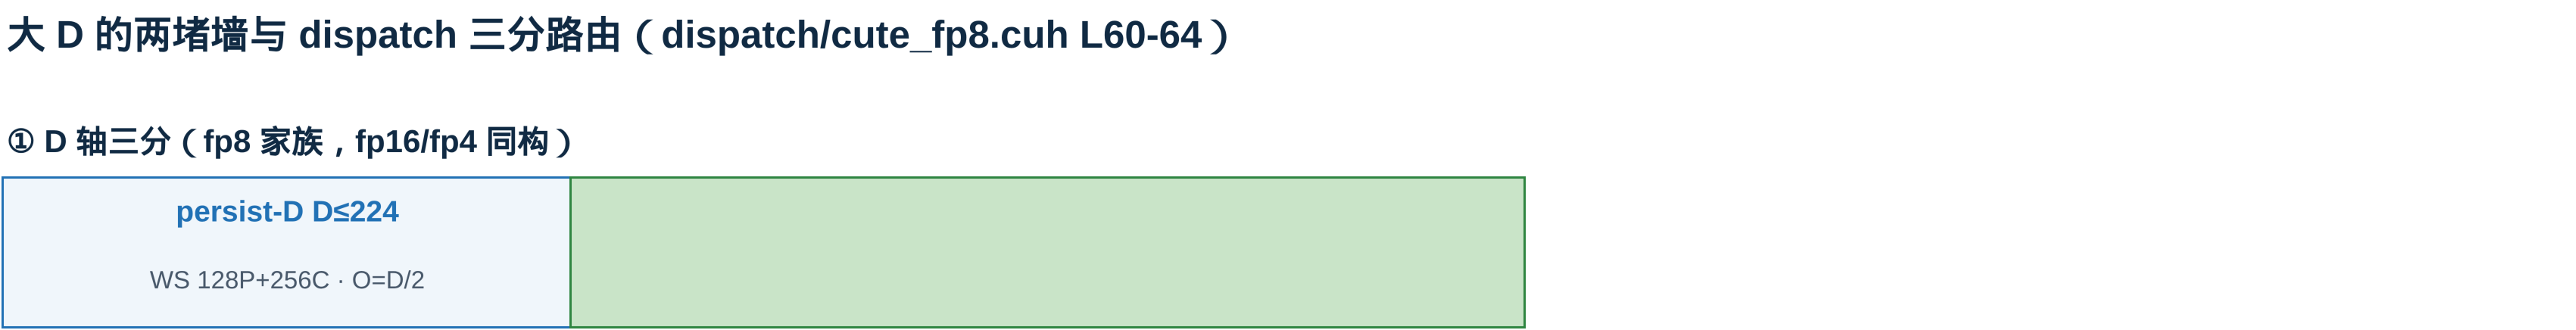
\includegraphics[width=0.98\textwidth]{figures/drawio/fig-30-1-split-d-walls/fig-30-1-split-d-walls.png}
  \begin{tikzpicture}
    \node[anchor=west, inner sep=0pt, align=left, font={\fontsize{7.4}{9.3}\selectfont \bfseries }] at (0.37,-0.354) {大 D 的两个瓶颈与 dispatch 三分路由（dispatch/cute\_fp8.cuh L60-64）};% w=17.433
    \node[anchor=west, inner sep=0pt, align=left, font={\fontsize{6.1}{7.7}\selectfont \bfseries }] at (0.37,-1.078) {(1) D 轴三分（fp8 家族，fp16/fp4 同构）};% w=4.620
    \node[draw=tkBlue, fill=tkFillBlue, line width=0.5pt, minimum width=3.85cm, minimum height=1.02cm, inner sep=1pt, align=center, text width=3.79cm, font={\fontsize{5.7}{7.1}\selectfont }] at (2.295,-1.833) {};
    \node[anchor=center, inner sep=0pt, align=center, font={\fontsize{5.7}{7.1}\selectfont \bfseries \color{tkBlue} }] at (2.295,-1.555) {persist-D  D$\leq$224};% w=3.665
    \node[anchor=center, inner sep=0pt, align=center, font={\fontsize{4.8}{6.0}\selectfont \color{black!65} }] at (2.295,-2.017) {WS 128P+256C $\cdot$ O=D/2};% w=3.665
    \node[draw=tkGreen, fill=tkFillGreen, line width=0.5pt, minimum width=6.47cm, minimum height=1.02cm, inner sep=1pt, align=center, text width=6.41cm, font={\fontsize{5.7}{7.1}\selectfont }] at (7.454,-1.833) {};
    \node[anchor=center, inner sep=0pt, align=center, font={\fontsize{5.7}{7.1}\selectfont \bfseries \color{tkGreen!70!black} }] at (7.454,-1.555) {split-D M8N1  224$<$D$<$768};% w=6.283
    \node[anchor=center, inner sep=0pt, align=center, font={\fontsize{4.8}{6.0}\selectfont \color{black!65} }] at (7.454,-2.017) {kBr/kBc=128/128 $\cdot$ non-WS 256T $\cdot$ O=D/2};% w=6.283
    \node[draw=tkOrange, fill=tkFillOrange, line width=0.5pt, minimum width=7.39cm, minimum height=1.02cm, inner sep=1pt, align=center, text width=7.33cm, font={\fontsize{5.7}{7.1}\selectfont }] at (13.614,-1.833) {};
    \node[anchor=center, inner sep=0pt, align=center, font={\fontsize{5.7}{7.1}\selectfont \bfseries \color{tkOrange} }] at (13.614,-1.555) {split-D M4N2  D$\geq$768};% w=7.207
    \node[anchor=center, inner sep=0pt, align=center, font={\fontsize{4.8}{6.0}\selectfont \color{black!65} }] at (13.614,-2.017) {kBr/kBc=64/64 $\cdot$ non-WS 256T $\cdot$ O=D/4};% w=7.207
    \node[anchor=center, inner sep=0pt, align=center, font={\fontsize{5.2}{6.6}\selectfont \bfseries }] at (11.15,-1.001) {交叉点 D=768};% w=2.464
    \node[draw=tkRed, fill=tkFillRed, line width=0.5pt, minimum width=8.32cm, minimum height=2.62cm, inner sep=1pt, align=center, text width=8.25cm, font={\fontsize{5.7}{7.1}\selectfont }] at (4.528,-4.235) {};
    \node[anchor=west, inner sep=0pt, align=left, font={\fontsize{6.1}{7.7}\selectfont \bfseries \color{tkRed} }] at (0.616,-3.219) {瓶颈一 smem：K tile 字节 = Bc$\times$D$\times$1B，O(D)};% w=7.823
    \node[anchor=west, inner sep=0pt, align=left, font={\fontsize{5.2}{6.6}\selectfont }] at (0.616,-3.634) {D=512、Bc=128 $\to$ K tile 64KB；加 V stage + Q 即超 99KB 预算};% w=7.823
    \node[anchor=west, inner sep=0pt, align=left, font={\fontsize{5.2}{6.6}\selectfont }] at (0.616,-4.004) {persist-D 的 K stage-0 复用只在 D$\leq$224 装得下};% w=7.823
    \node[draw=tkRed, fill=none, line width=0.5pt, minimum width=3.70cm, minimum height=0.95cm, inner sep=1pt, align=center, text width=3.63cm, font={\fontsize{5.2}{6.6}\selectfont }] at (2.464,-4.759) {整块 K tile 一次进 smem\\（persist-D：D$\leq$224 专属）};
    \node[draw=tkGreen, fill=none, line width=0.5pt, minimum width=3.70cm, minimum height=0.95cm, inner sep=1pt, align=center, text width=3.63cm, font={\fontsize{5.2}{6.6}\selectfont \bfseries \color{tkGreen!70!black} }] at (6.468,-4.759) {split-D：D 切 chunk 流水\\每 stage 与总 D 无关};
    \node[anchor=west, inner sep=0pt, align=left, font={\fontsize{4.8}{6.0}\selectfont \color{black!55} }] at (0.616,-5.405) {chunk\_index = kv\_tile$\cdot$kDChunks + c，stage/phase 环形推进};% w=7.823
    \node[draw=tkPurple, fill=tkFillPurple, line width=0.5pt, minimum width=8.62cm, minimum height=2.62cm, inner sep=1pt, align=center, text width=8.56cm, font={\fontsize{5.7}{7.1}\selectfont }] at (13.49,-4.235) {};
    \node[anchor=west, inner sep=0pt, align=left, font={\fontsize{6.1}{7.7}\selectfont \bfseries \color{tkPurple} }] at (9.425,-3.219) {瓶颈二 寄存器：O 累加器 = D/(2N\_w) f32/线程};% w=8.131
    \node[anchor=west, inner sep=0pt, align=left, font={\fontsize{5.2}{6.6}\selectfont }] at (9.425,-3.634) {M8N1 单 warp 独占整 D 列：D=512 $\to$ 256 regs 超上限（255）};% w=8.131
    \node[anchor=west, inner sep=0pt, align=left, font={\fontsize{5.2}{6.6}\selectfont }] at (9.425,-4.004) {D$\geq$896 大量 spill（D=1024 实测 \textasciitilde{}100T）};% w=8.131
    \node[draw=tkPurple, fill=none, line width=0.5pt, minimum width=3.85cm, minimum height=0.95cm, inner sep=1pt, align=center, text width=3.79cm, font={\fontsize{5.2}{6.6}\selectfont }] at (11.35,-4.759) {M8N1 (8,1,1)：O=D/2\\D=1024 $\to$ 512 regs 溢出};
    \node[draw=tkOrange, fill=none, line width=0.5pt, minimum width=3.85cm, minimum height=0.95cm, inner sep=1pt, align=center, text width=3.79cm, font={\fontsize{5.2}{6.6}\selectfont \bfseries \color{tkOrange!75!black} }] at (15.508,-4.759) {M4N2 (4,2,1)：O=D/4\\D=1024 $\to$ 256 regs 边缘 spill 154T};
    \node[draw=gray!55, fill=black!2, line width=0.5pt, minimum width=17.43cm, minimum height=2.31cm, inner sep=1pt, align=center, text width=17.37cm, font={\fontsize{5.7}{7.1}\selectfont }] at (9.086,-7.253) {};
    \node[anchor=west, inner sep=0pt, align=left, font={\fontsize{6.1}{7.7}\selectfont \bfseries }] at (0.616,-6.391) {(2) 寄存器压力模型：N\_w 消去，只有减 M\_w 有效};% w=16.940
    \node[anchor=west, inner sep=0pt, align=left, font={\fontsize{5.7}{7.1}\selectfont }] at (0.616,-6.868) {per-thread：O\_acc = 4$\cdot$(kBr/16M\_w)$\cdot$(D/8N\_w)/(kBr/16M\_w) = D/(2N\_w)};% w=9.856
    \node[anchor=west, inner sep=0pt, align=left, font={\fontsize{5.7}{7.1}\selectfont \bfseries \color{tkPurple} }] at (0.616,-7.269) {per-SM 池占比：[D/(2N\_w)] / [65536/(32M\_wN\_w)] = D$\cdot$M\_w/4096};% w=9.856
    \node[anchor=west, inner sep=0pt, align=left, font={\fontsize{5.2}{6.6}\selectfont \color{black!65} }] at (0.616,-7.669) {N\_w 精确消去：M4N4 $\equiv$ M4N2（同为 D/1024）；M2N4 $\to$ D/2048 是 D$>$1024 正解};% w=9.856
    \node[anchor=west, inner sep=0pt, align=left, font={\fontsize{5.2}{6.6}\selectfont \bfseries \color{tkRed} }] at (10.965,-7.099) {被否决的捷径(1)：QK M8N1 + PV M4N2 混合布局};% w=6.591
    \node[anchor=west, inner sep=0pt, align=left, font={\fontsize{4.8}{6.0}\selectfont }] at (10.965,-7.623) {QK/PV 共享 Q tile，M 维须一致：\\kBr=128 $\to$ PV 仍 D/2\\kBr=64 $\to$ M8N1 空 4 warp};% w=6.591
    \node[anchor=west, inner sep=0pt, align=left, font={\fontsize{5.2}{6.6}\selectfont \bfseries \color{tkRed} }] at (10.965,-8.177) {被否决的捷径(2)：WS 版 split-D};% w=6.591
    \node[anchor=west, inner sep=0pt, align=left, font={\fontsize{4.8}{6.0}\selectfont }] at (10.965,-8.747) {setmaxnreg 上限 232 装不下 D=512 的 256-reg O};% w=6.591
    \node[draw=tkGreen, fill=tkFillGreen, line width=0.5pt, minimum width=17.43cm, minimum height=2.31cm, inner sep=1pt, align=center, text width=17.37cm, font={\fontsize{5.7}{7.1}\selectfont }] at (9.086,-10.025) {};
    \node[anchor=west, inner sep=0pt, align=left, font={\fontsize{6.1}{7.7}\selectfont \bfseries \color{tkGreen!70!black} }] at (0.616,-9.163) {(3) 实测交叉点（5090，fp16 同构；PRO 5000 数据见正文 30.6）};% w=16.940
    \node[anchor=west, inner sep=0pt, align=left, font={\fontsize{5.2}{6.6}\selectfont }] at (0.616,-9.579) {D$\leq$640：M8N1 快 +2\textasciitilde{}16\%（无 P roundtrip、kBr 大一倍）};% w=8.316
    \node[anchor=west, inner sep=0pt, align=left, font={\fontsize{5.2}{6.6}\selectfont \bfseries }] at (0.616,-9.948) {D$\geq$768：M4N2 快 +7\%@768、+11\%@896、+55\%@1024};% w=8.316
    \node[anchor=west, inner sep=0pt, align=left, font={\fontsize{5.2}{6.6}\selectfont \color{black!55} }] at (0.616,-10.318) {FFPA\_FP8\_FORCE\_KERNEL=split\_d|m4n2（224$<$D$\leq$1024）可强制 A/B};% w=8.316
    \node[anchor=west, inner sep=0pt, align=left, font={\fontsize{5.2}{6.6}\selectfont \color{black!55} }] at (0.616,-10.688) {PRO 5000 实测（本机 headdim 止于 512）：D=512 self 203T / 2.98x};% w=8.316
    \node[anchor=west, inner sep=0pt, align=left, font={\fontsize{5.7}{7.1}\selectfont \bfseries \color{tkGreen!70!black} }] at (9.548,-9.579) {split-D 是精确变换：};% w=8.008
    \node[anchor=west, inner sep=0pt, align=left, font={\fontsize{5.2}{6.6}\selectfont }] at (9.548,-9.948) {QK 侧 D 是归约维：$\Sigma$\_c Q\_c K\_c\^{}T 累加进同一 S（无新舍入点）};% w=8.008
    \node[anchor=west, inner sep=0pt, align=left, font={\fontsize{5.2}{6.6}\selectfont }] at (9.548,-10.318) {PV 侧 D 是输出列维：各 chunk 的 O 段独立累加};% w=8.008
    \node[anchor=west, inner sep=0pt, align=left, font={\fontsize{5.2}{6.6}\selectfont \bfseries }] at (9.548,-10.688) {softmax 行统计 (m,$\ell$) 是 KV 行维的量------与 D 切分无关};% w=8.008
    \draw[black!75, line width=0.8pt, dashed] (9.918,-1.14) -- (9.918,-2.464);
    \draw[gray!55, line width=0.5pt, dashed] (4.22,-1.14) -- (4.22,-2.464);
    \draw[tkGreen, line width=0.8pt, -{Stealth[length=2.2pt,width=1.8pt]}] (4.312,-4.759) -- (4.62,-4.759);
    \draw[tkOrange, line width=0.8pt, -{Stealth[length=2.2pt,width=1.8pt]}] (13.275,-4.759) -- (13.583,-4.759);
    \draw[gray!55, line width=0.5pt] (10.718,-6.714) -- (10.718,-8.1);
    \draw[gray!55, line width=0.5pt] (9.302,-9.425) -- (9.302,-10.842);
  \end{tikzpicture}
  \caption{大 $D$ 的两个瓶颈与 dispatch 三分路由。smem 瓶颈由 split-D 解决
  （chunk 流水，smem 与 $D$ 解耦）；寄存器瓶颈由 M4N2 解决（$N_w=2$ 把
  per-thread $O$ 从 $D/2$ 减到 $D/4$）；$D=768$ 是实测交叉点。}
  \label{fig:30-walls}
\end{figure}

\begin{figure}[htbp]
  \centering
  % was: 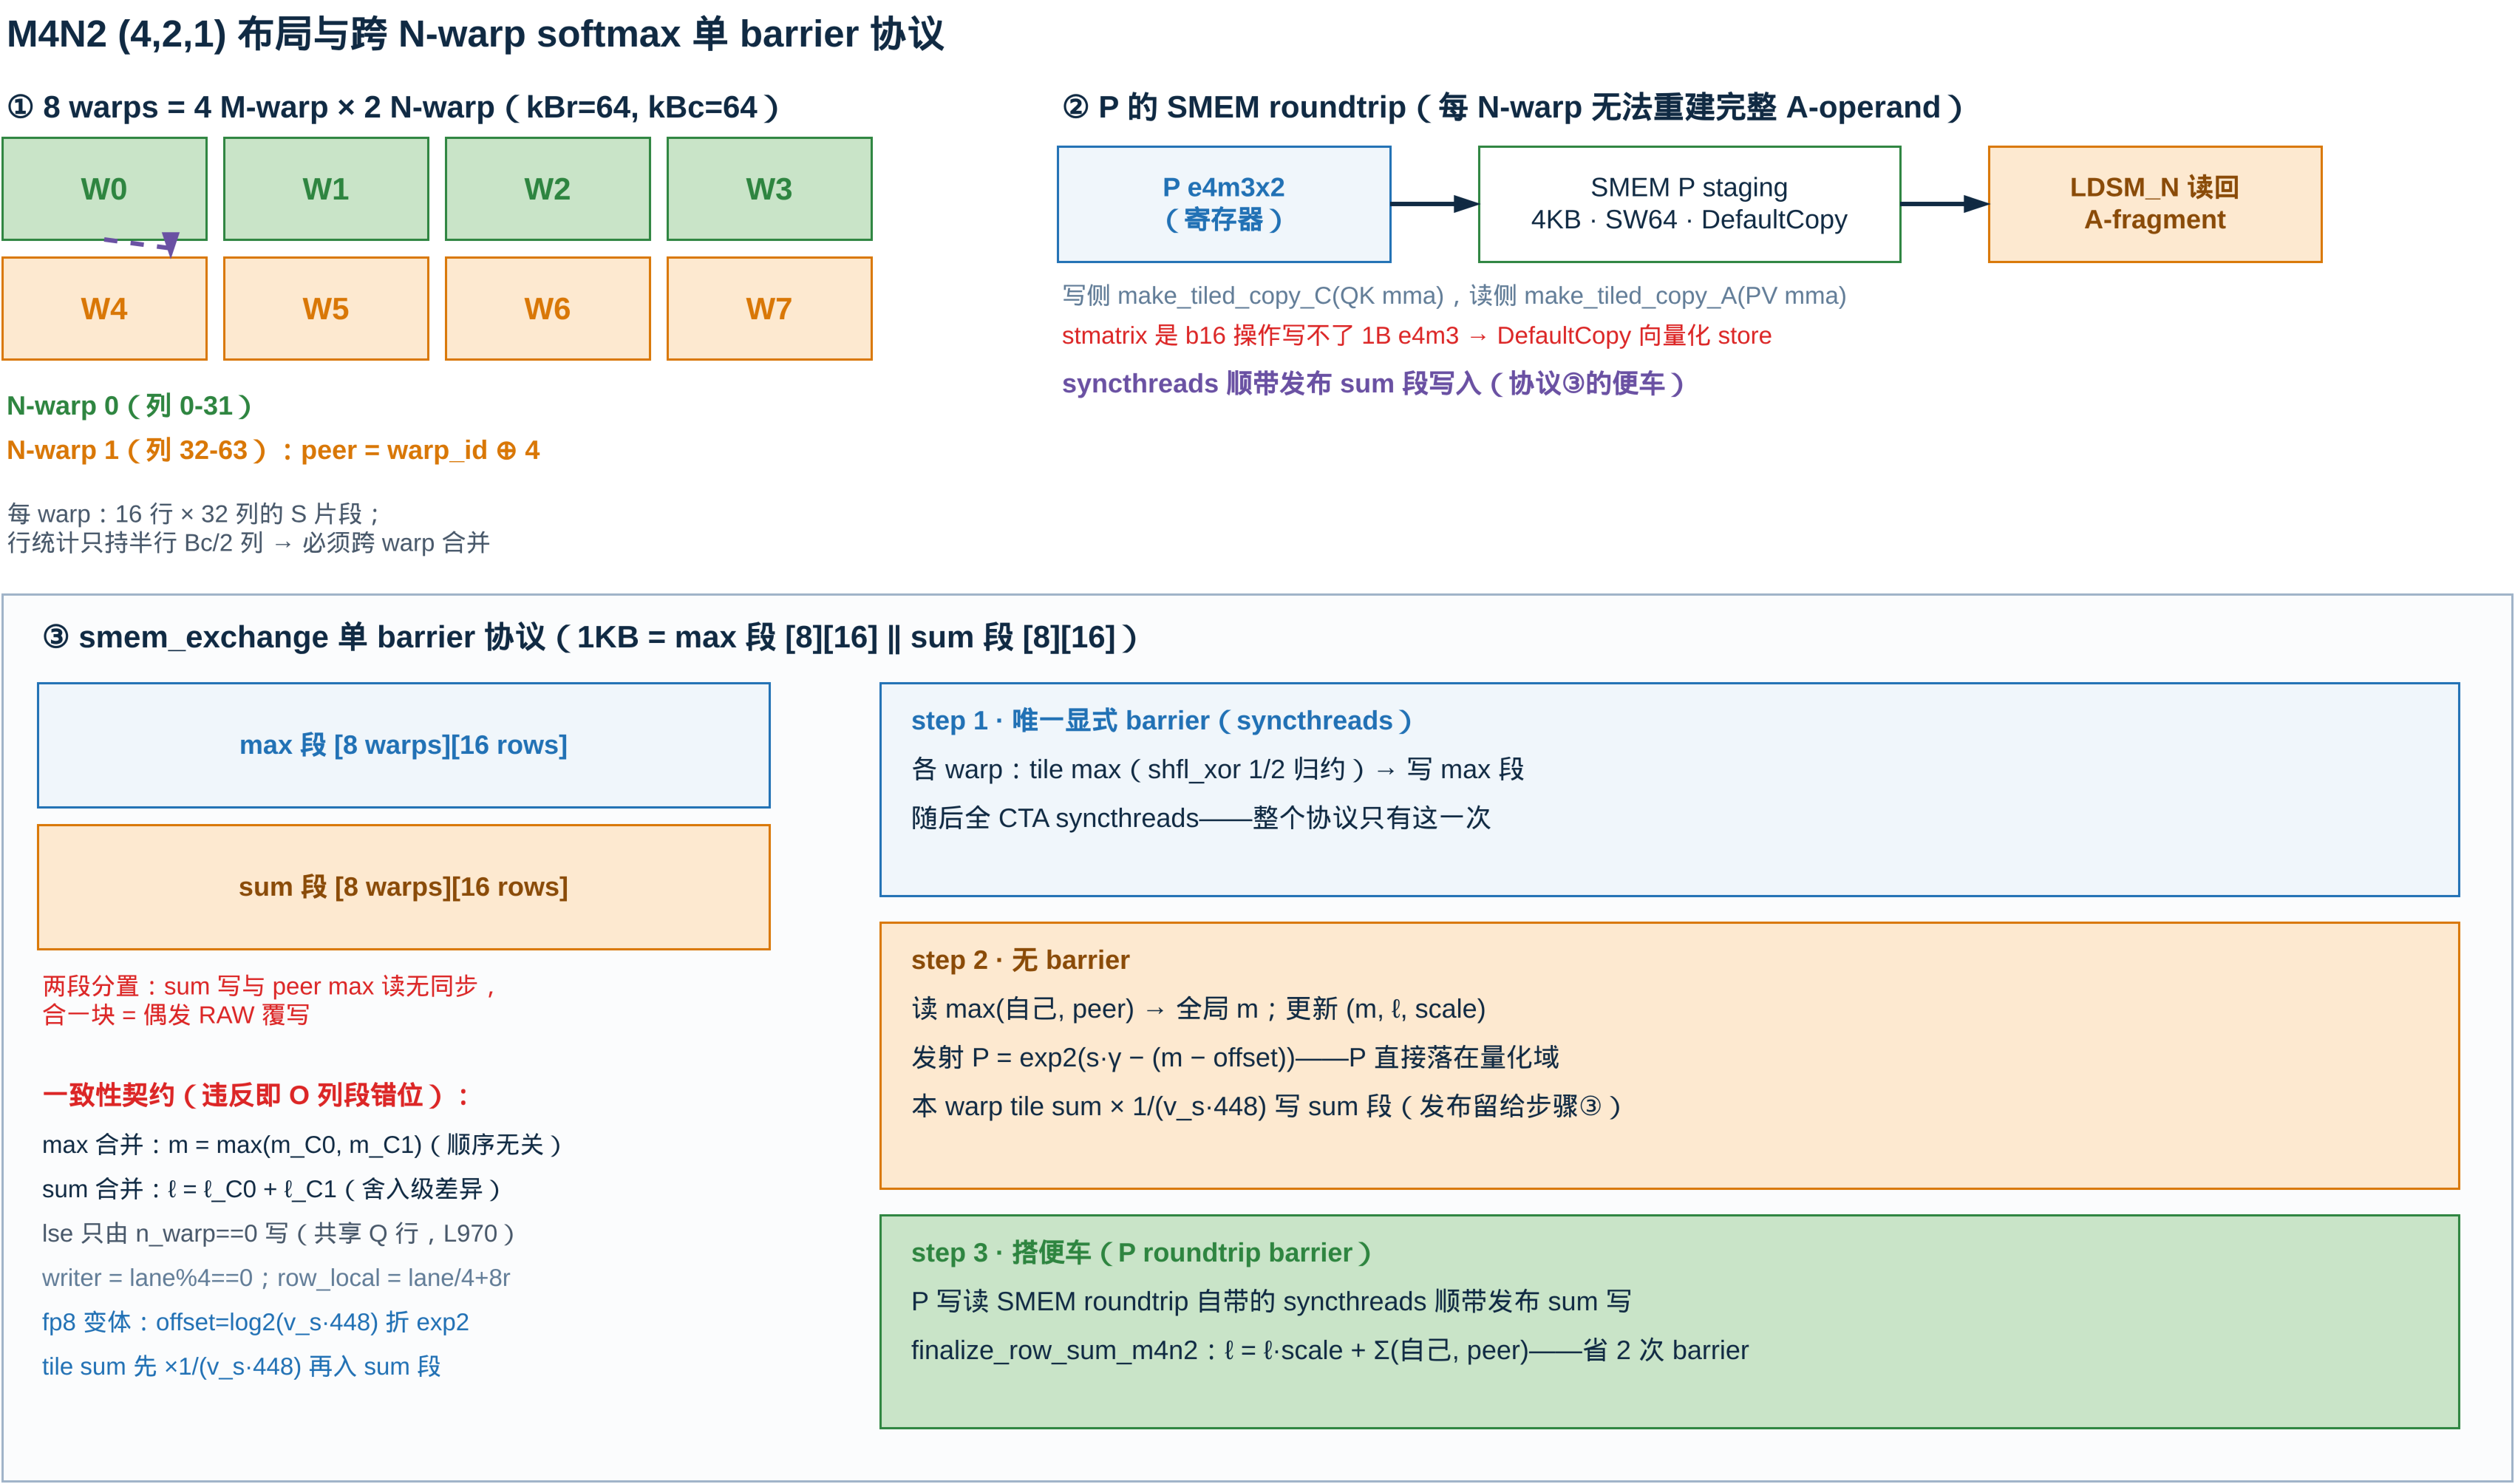
\includegraphics[width=0.98\textwidth]{figures/drawio/fig-30-2-m4n2-softmax/fig-30-2-m4n2-softmax.png}
  \begin{tikzpicture}
    \node[anchor=west, inner sep=0pt, align=left, font={\fontsize{7.4}{9.3}\selectfont \bfseries }] at (0.37,-0.354) {M4N2 (4,2,1) 布局与跨 N-warp softmax 单 barrier 协议};% w=17.433
    \node[anchor=west, inner sep=0pt, align=left, font={\fontsize{5.6}{7.0}\selectfont \bfseries }] at (0.37,-0.862) {(1) 8 warps = 4 M-warp $\times$ 2 N-warp（kBr=64, kBc=64）};% w=8.624
    \node[draw=tkGreen, fill=tkFillGreen, line width=0.5pt, minimum width=1.42cm, minimum height=0.71cm, inner sep=1pt, align=center, text width=1.36cm, font={\fontsize{6.1}{7.7}\selectfont \bfseries \color{tkGreen!70!black} }] at (1.078,-1.432) {W0};
    \node[draw=tkGreen, fill=tkFillGreen, line width=0.5pt, minimum width=1.42cm, minimum height=0.71cm, inner sep=1pt, align=center, text width=1.36cm, font={\fontsize{6.1}{7.7}\selectfont \bfseries \color{tkGreen!70!black} }] at (2.618,-1.432) {W1};
    \node[draw=tkGreen, fill=tkFillGreen, line width=0.5pt, minimum width=1.42cm, minimum height=0.71cm, inner sep=1pt, align=center, text width=1.36cm, font={\fontsize{6.1}{7.7}\selectfont \bfseries \color{tkGreen!70!black} }] at (4.158,-1.432) {W2};
    \node[draw=tkGreen, fill=tkFillGreen, line width=0.5pt, minimum width=1.42cm, minimum height=0.71cm, inner sep=1pt, align=center, text width=1.36cm, font={\fontsize{6.1}{7.7}\selectfont \bfseries \color{tkGreen!70!black} }] at (5.698,-1.432) {W3};
    \node[draw=tkOrange, fill=tkFillOrange, line width=0.5pt, minimum width=1.42cm, minimum height=0.71cm, inner sep=1pt, align=center, text width=1.36cm, font={\fontsize{6.1}{7.7}\selectfont \bfseries \color{tkOrange} }] at (1.078,-2.264) {W4};
    \node[draw=tkOrange, fill=tkFillOrange, line width=0.5pt, minimum width=1.42cm, minimum height=0.71cm, inner sep=1pt, align=center, text width=1.36cm, font={\fontsize{6.1}{7.7}\selectfont \bfseries \color{tkOrange} }] at (2.618,-2.264) {W5};
    \node[draw=tkOrange, fill=tkFillOrange, line width=0.5pt, minimum width=1.42cm, minimum height=0.71cm, inner sep=1pt, align=center, text width=1.36cm, font={\fontsize{6.1}{7.7}\selectfont \bfseries \color{tkOrange} }] at (4.158,-2.264) {W6};
    \node[draw=tkOrange, fill=tkFillOrange, line width=0.5pt, minimum width=1.42cm, minimum height=0.71cm, inner sep=1pt, align=center, text width=1.36cm, font={\fontsize{6.1}{7.7}\selectfont \bfseries \color{tkOrange} }] at (5.698,-2.264) {W7};
    \node[anchor=west, inner sep=0pt, align=left, font={\fontsize{5.2}{6.6}\selectfont \bfseries \color{tkGreen!70!black} }] at (0.37,-2.941) {N-warp 0（列 0-31）};% w=6.406
    \node[anchor=west, inner sep=0pt, align=left, font={\fontsize{5.2}{6.6}\selectfont \bfseries \color{tkOrange} }] at (0.37,-3.249) {N-warp 1（列 32-63）：peer = warp\_id $\oplus$ 4};% w=6.406
    \node[anchor=west, inner sep=0pt, align=left, font={\fontsize{4.8}{6.0}\selectfont \color{black!65} }] at (0.37,-3.788) {每 warp：16 行 $\times$ 32 列的 S 片段；\\行统计只持半行 Bc/2 列 $\to$ 必须跨 warp 合并};% w=6.622
    \node[anchor=west, inner sep=0pt, align=left, font={\fontsize{6.1}{7.7}\selectfont \bfseries }] at (7.7,-0.862) {(2) P 的 SMEM roundtrip（每 N-warp 无法重建完整 A-operand）};% w=10.102
    \node[draw=tkBlue, fill=tkFillBlue, line width=0.5pt, minimum width=2.31cm, minimum height=0.80cm, inner sep=1pt, align=center, text width=2.25cm, font={\fontsize{5.2}{6.6}\selectfont \bfseries \color{tkBlue} }] at (8.855,-1.54) {P e4m3x2\\（寄存器）};
    \node[draw=tkGreen, fill=none, line width=0.5pt, minimum width=2.93cm, minimum height=0.80cm, inner sep=1pt, align=center, text width=2.86cm, font={\fontsize{5.0}{6.3}\selectfont }] at (12.089,-1.54) {SMEM P staging\\4KB $\cdot$ SW64 $\cdot$ DefaultCopy};
    \node[draw=tkOrange, fill=tkFillOrange, line width=0.5pt, minimum width=2.31cm, minimum height=0.80cm, inner sep=1pt, align=center, text width=2.25cm, font={\fontsize{5.2}{6.6}\selectfont \bfseries \color{tkOrange!75!black} }] at (15.323,-1.54) {LDSM\_N 读回\\A-fragment};
    \node[anchor=west, inner sep=0pt, align=left, font={\fontsize{4.8}{6.0}\selectfont \color{black!55} }] at (7.7,-2.171) {写侧 make\_tiled\_copy\_C(QK mma)，读侧 make\_tiled\_copy\_A(PV mma)};% w=8.778
    \node[anchor=west, inner sep=0pt, align=left, font={\fontsize{4.8}{6.0}\selectfont \color{tkRed} }] at (7.7,-2.449) {stmatrix 是 b16 操作写不了 1B e4m3 $\to$ DefaultCopy 向量化 store};% w=8.778
    \node[anchor=west, inner sep=0pt, align=left, font={\fontsize{5.2}{6.6}\selectfont \bfseries \color{tkPurple} }] at (7.7,-2.787) {syncthreads 顺带发布 sum 段写入（复用协议(3) barrier）};% w=8.778
    \node[draw=gray!55, fill=black!2, line width=0.5pt, minimum width=17.43cm, minimum height=6.16cm, inner sep=1pt, align=center, text width=17.37cm, font={\fontsize{5.7}{7.1}\selectfont }] at (9.086,-7.33) {};
    \node[anchor=west, inner sep=0pt, align=left, font={\fontsize{6.1}{7.7}\selectfont \bfseries }] at (0.616,-4.543) {(3) smem\_exchange 单 barrier 协议（1KB = max 段 [8][16] $\|$ sum 段 [8][16]）};% w=16.940
    \node[draw=tkBlue, fill=tkFillBlue, line width=0.5pt, minimum width=5.08cm, minimum height=0.86cm, inner sep=1pt, align=center, text width=5.02cm, font={\fontsize{5.2}{6.6}\selectfont \bfseries \color{tkBlue} }] at (3.157,-5.298) {max 段 [8 warps][16 rows]};
    \node[draw=tkOrange, fill=tkFillOrange, line width=0.5pt, minimum width=5.08cm, minimum height=0.86cm, inner sep=1pt, align=center, text width=5.02cm, font={\fontsize{5.2}{6.6}\selectfont \bfseries \color{tkOrange!75!black} }] at (3.157,-6.283) {sum 段 [8 warps][16 rows]};
    \node[anchor=west, inner sep=0pt, align=left, font={\fontsize{4.8}{6.0}\selectfont \color{tkRed} }] at (0.616,-7.069) {两段分置：sum 写与 peer max 读无同步，\\合一块 = 偶发 RAW 覆写};% w=5.174
    \node[anchor=west, inner sep=0pt, align=left, font={\fontsize{5.2}{6.6}\selectfont \bfseries \color{tkRed} }] at (0.616,-7.731) {一致性约定（违反即 O 列段错位）：};% w=5.236
    \node[anchor=west, inner sep=0pt, align=left, font={\fontsize{4.8}{6.0}\selectfont }] at (0.616,-8.07) {max 合并：m = max(m\_C0, m\_C1)（顺序无关）};% w=5.236
    \node[anchor=west, inner sep=0pt, align=left, font={\fontsize{4.8}{6.0}\selectfont }] at (0.616,-8.378) {sum 合并：$\ell$ = $\ell$\_C0 + $\ell$\_C1（舍入级差异）};% w=5.236
    \node[anchor=west, inner sep=0pt, align=left, font={\fontsize{4.8}{6.0}\selectfont \color{black!65} }] at (0.616,-8.686) {lse 只由 n\_warp==0 写（共享 Q 行，L970）};% w=5.236
    \node[anchor=west, inner sep=0pt, align=left, font={\fontsize{4.8}{6.0}\selectfont \color{black!55} }] at (0.616,-8.994) {writer = lane\%4==0；row\_local = lane/4+8r};% w=5.236
    \node[anchor=west, inner sep=0pt, align=left, font={\fontsize{4.8}{6.0}\selectfont \color{tkBlue} }] at (0.616,-9.302) {fp8 变体：offset=log2(v\_s$\cdot$448) 折 exp2};% w=5.236
    \node[anchor=west, inner sep=0pt, align=left, font={\fontsize{4.8}{6.0}\selectfont \color{tkBlue} }] at (0.616,-9.61) {tile sum 先 $\times$1/(v\_s$\cdot$448) 再入 sum 段};% w=5.236
    \node[draw=tkBlue, fill=tkFillBlue, line width=0.5pt, minimum width=10.96cm, minimum height=1.48cm, inner sep=1pt, align=center, text width=10.90cm, font={\fontsize{5.7}{7.1}\selectfont }] at (11.95,-5.606) {};
    \node[anchor=west, inner sep=0pt, align=left, font={\fontsize{5.2}{6.6}\selectfont \bfseries \color{tkBlue} }] at (6.653,-5.128) {step 1 $\cdot$ 唯一显式 barrier（syncthreads）};% w=10.595
    \node[anchor=west, inner sep=0pt, align=left, font={\fontsize{5.2}{6.6}\selectfont }] at (6.653,-5.467) {各 warp：tile max（shfl\_xor 1/2 归约）$\to$ 写 max 段};% w=10.595
    \node[anchor=west, inner sep=0pt, align=left, font={\fontsize{5.2}{6.6}\selectfont }] at (6.653,-5.806) {随后全 CTA syncthreads------整个协议只有这一次};% w=10.595
    \node[draw=tkOrange, fill=tkFillOrange, line width=0.5pt, minimum width=10.96cm, minimum height=1.85cm, inner sep=1pt, align=center, text width=10.90cm, font={\fontsize{5.7}{7.1}\selectfont }] at (11.95,-7.454) {};
    \node[anchor=west, inner sep=0pt, align=left, font={\fontsize{5.2}{6.6}\selectfont \bfseries \color{tkOrange!75!black} }] at (6.653,-6.791) {step 2 $\cdot$ 无 barrier};% w=10.595
    \node[anchor=west, inner sep=0pt, align=left, font={\fontsize{5.2}{6.6}\selectfont }] at (6.653,-7.13) {读 max(自己, peer) $\to$ 全局 m；更新 (m, $\ell$, scale)};% w=10.595
    \node[anchor=west, inner sep=0pt, align=left, font={\fontsize{5.2}{6.6}\selectfont }] at (6.653,-7.469) {发射 P = exp2(s$\cdot$$\gamma$ $-$ (m $-$ offset))------P 直接落在量化域};% w=10.595
    \node[anchor=west, inner sep=0pt, align=left, font={\fontsize{5.2}{6.6}\selectfont }] at (6.653,-7.808) {本 warp tile sum $\times$ 1/(v\_s$\cdot$448) 写 sum 段（发布留给步骤(3)）};% w=10.595
    \node[draw=tkGreen, fill=tkFillGreen, line width=0.5pt, minimum width=10.96cm, minimum height=1.48cm, inner sep=1pt, align=center, text width=10.90cm, font={\fontsize{5.7}{7.1}\selectfont }] at (11.95,-9.302) {};
    \node[anchor=west, inner sep=0pt, align=left, font={\fontsize{5.2}{6.6}\selectfont \bfseries \color{tkGreen!70!black} }] at (6.653,-8.824) {step 3 $\cdot$ 复用 P roundtrip barrier};% w=10.595
    \node[anchor=west, inner sep=0pt, align=left, font={\fontsize{5.2}{6.6}\selectfont }] at (6.653,-9.163) {P 写读 SMEM roundtrip 自带的 syncthreads 顺带发布 sum 写};% w=10.595
    \node[anchor=west, inner sep=0pt, align=left, font={\fontsize{5.2}{6.6}\selectfont }] at (6.653,-9.502) {finalize\_row\_sum\_m4n2：$\ell$ = $\ell$$\cdot$scale + $\Sigma$(自己, peer)------复用后净省 1 次 barrier};% w=10.595
    \draw[tkPurple, line width=0.8pt, dashed, -{Stealth[length=2.2pt,width=1.8pt]}] (1.078,-1.786) -- (1.54,-1.848) -- (1.54,-1.91);
    \draw[black!75, line width=0.8pt, -{Stealth[length=2.2pt,width=1.8pt]}] (10.01,-1.54) -- (10.626,-1.54);
    \draw[black!75, line width=0.8pt, -{Stealth[length=2.2pt,width=1.8pt]}] (13.552,-1.54) -- (14.168,-1.54);
  \end{tikzpicture}
  \caption{M4N2 的 $(4,2,1)$ atom 布局与跨 N-warp softmax 单 barrier
  协议。max 段与 sum 段分置 \texttt{smem\_exchange} 防 RAW；sum 写入的
  发布复用 P roundtrip 的 barrier。}
  \label{fig:30-m4n2}
\end{figure}

\FloatBarrier

\section{性能分析}

\subsection{本机实测（RTX PRO 5000，B1 H32 N8192，bench 默认配置）}

命令：
\begin{lstlisting}[style=console,aboveskip=4pt,belowskip=2pt]
export CUDA_VISIBLE_DEVICES=7 FFPA_CUDA_ALLOW_SMALL_D=1
python -m ffpa_attn.bench --fwd-backend cuda --cuda-impl fp8 \
  --tasks self-attn,causal --D {256,320,512} --no-bwd --show-allclose
\end{lstlisting}

\begin{center}
\begin{tabular}{@{}llrrrl@{}}
\toprule
$D$ & task & FFPA ms & SDPA ms & TFLOPS & speedup \\
\midrule
256 & self   & 8.12  & 10.52 & 271T & 1.30x \\
256 & causal & 4.73  & 5.29  & 233T & 1.12x \\
320 & self   & 10.71 & 40.25 & 257T & 3.76x \\
320 & causal & 6.23  & 20.61 & 221T & 3.31x \\
512 & self   & 21.71 & 64.74 & 203T & 2.98x \\
512 & causal & 12.82 & 32.92 & 172T & 2.57x \\
\bottomrule
\end{tabular}
\end{center}

self-attn 的 speedup 从 $D=256$ 的 1.30x 跳到
$D=320$ 的 3.76x，拐点不在 kernel 而在参照系：SDPA 在
$D\notin\{64,128\}$ 时不再命中最优 kernel，fp8 的 1B 元素带宽优势
立即显现。TFLOPS 随 $D$ 单调下降（271$\to$203T），主要对应 $O$ 寄存器压力、
chunk 握手与 epilogue staging 开销。softmax 与 P 量化等 $O(B_c)$ 项成本不随
$D$ 增长，其相对占比反而下降，不能用来解释这一趋势。causal 的 allclose 在 D=320 bf16 与
D=512 fp16 两格临界失败（见 30.2.3~节的已知边界说明），dense 六格
全绿，数据落盘 \texttt{.tmp/book-bench/ch30/}。

\subsection{交叉点与 M4N2 的引用数据（本机无 $D\ge768$ 编译实例）}

本机 headdim 编译集止于 512，M4N2 只能引用 5090 数据（fp16 家族同构、
同一 dispatch 交叉点）：$D\le640$ 时 M8N1 快 $2\sim16\%$；
$D\ge768$ 时 M4N2 快 $+7\%@768$、$+11\%@896$、$+55\%@1024$。劣化一侧
的数字更说明问题：$D=1024$ 时 M8N1 的 $O_{\text{acc}}=512$ regs
溢出 local memory，吞吐 $\sim$100T；M4N2 同 $D$ 边缘 spill 仍有
154T。\texttt{FFPA\_FP8\_FORCE\_KERNEL=split\_d|m4n2}（$224<D\le1024$，
\texttt{dispatch/cute\_fp8.cuh} L24--33，仅在 \texttt{--debug-ext fp8}
的 debug 构建里生效）可在有 768+ 编译实例的
机器上强制 A/B 复现交叉点。

\subsection{roofline 视角}

fp8 split-D 在 $D=512$ 的 203T 大约是 fp8 persist-D 峰值（365T，
第~\ref{ch:29}~章 29.6 节实测表）的 56\%。差距的构成：$O$ 累加器随 $D$ 翻倍的寄存器开销
（occupancy 1 CTA）、chunk 循环多出的 barrier 握手、以及 epilogue
批量 staging 的 smem 往返。这并不构成 split-D 的失败：绝对吞吐仍高于
fp16 家族同 $D$ 量级，1B/元素也确实降低搬运压力。但表中 $D{=}320$ 的
3.76x 是相对本 bench 在该形状选择 SDPA-MATH 的端到端比值，不能全部归因于
FP8 带宽优势。

\section{实践经验}

\subsection{案例：causal allclose 临界失败的定位与定性}

30.6~节表格里有两格 \texttt{allclose} 失败：D=320（bf16）、
D=512（fp16）。

定性过程记录如下，脚本在 \texttt{.tmp/book-bench/ch30/}：

\begin{enumerate}[itemsep=0pt,topsep=2pt]
  \item 先看模式不看标量。对 $D\in\{256,320,512\}$ 各跑
        causal，逐 512-行块统计超阈行占比：三者模式完全一致，
        前 $\sim$30\% 块 100\% 超阈、后段 0\%，max $\sim$2、
        mean $\sim$0.007；
  \item dense 对照：self-attn 六格全绿 $\Rightarrow$ 公共 chunk 流水与
        epilogue 未见结构性错误；dense 不执行 causal mask，因此不能据此
        排除 mask 错位，mask 仍需独立边界用例；
  \item 对照头注释。L40--43 声明的\textbf{causal 早期行
        attend 少、误差不被平均}与实测模式吻合：早期行
        $P$ 分布尖，e4m3 的 $2^{-4}$（半格）相对舍入直接进 $O$；行号
        过半后 $P$ 足够平，误差被平均掉；
  \item \textbf{结论}：现象与该实现的已知 ESS 精度特性一致，但 dense
        对照本身不构成“非回归 bug”的证明。需要严格 causal 精度的场景可走
        hybrid（前若干行 fp16 stage-1）；要排除回归，先补 mask 单元测试。
\end{enumerate}

这套流程（模式 $\to$ dense 对照 $\to$ 对照声明 $\to$ 定性）与
29.7.1~节 D=192 的定位流程同构：先区分 mask 回归与已知数值特性，再决定
修 kernel 还是采用 hybrid。

\subsection{什么时候不该学本章}

split-D/M4N2 是 $D>224$ 的\textbf{被迫选择}，不是普适更优。三条负面
证据：WS 版 split-D 被 setmaxnreg 232 上限否决；QK/PV 混合 atom 布局
被 M 维一致性否决；fused-rescale 在 split-D 域实测为负收益。三条都是
在 persist-D 域成立的优化不能照搬的实例，迁移优化前先核对 occupancy
与寄存器结构是否相同；进一步定位 fused-rescale 的执行瓶颈需另做 NCU。

\section{常见坑}

\begin{enumerate}[itemsep=2pt,topsep=2pt]
  \item \textbf{P roundtrip 写侧坐标系}：写侧必须从 QK 的
        \texttt{tiled\_mma\_qk} 构造 \texttt{make\_tiled\_copy\_C}，
        读侧从 PV 的 \texttt{tiled\_mma\_pv} 构造
        \texttt{make\_tiled\_copy\_A}；手写 A-operand 映射与 LDSM
        读侧不对称会产生错误数值（sm80 家族的实测教训，L685--698 用
        \texttt{DefaultCopy} 规避向量化陷阱）。
  \item \textbf{max/sum 同区覆写}：单 barrier 协议里 sum 写与 peer
        max 读之间没有同步，两段必须分置；合成一块省下的 512B 换来
        偶发 RAW 错值（softmax.cuh L92--95）。
  \item \textbf{stmatrix 写不了 1B e4m3}：它是 b16 操作；1B 元素的
        P staging 退回 \texttt{DefaultCopy} 向量化 store（L685--688）。
  \item \textbf{两套块宽不一致}：$k_{Br}=64$ vs 量化 128 行块，奇数
        tile 需要 \texttt{quant\_offset}/\texttt{quant\_rb} 重映射
        （L129、L300--307）；漏掉的行查到邻块的 scale，误差温和到
        很难肉眼发现。
  \item \textbf{kSmemElems 的单位}：fp8 traits 里它数 1B 元素恰等于
        字节数；O staging 断言要乘 \texttt{sizeof(ElementO)}，否则
        预算虚大一倍（L105--108）。
  \item \textbf{stage 下限的家族差异}：persist-D 抬 stages 已证伪、
        m4n2 抬到 3 是全局最优——差别只在 occupancy 是否已被限制；
        跨家族照搬 stage 配置前先想清楚这一条。
\end{enumerate}

\section{面试要点速查}

\begin{enumerate}[itemsep=2pt,topsep=2pt]
  \item \textbf{split-D 为什么精确}？QK 侧 $D$ 是归约维，chunk 累加
        进同一 fragment（式~\ref{eq:30-qk-split}）；PV 侧是输出列维，
        各 chunk 独立（式~\ref{eq:30-pv-split}）；softmax 行统计与
        $D$ 切分无关，不产生 per-chunk 的 $(m,\ell)$。
  \item \textbf{M4N2 减的是哪一维}？$N$ 维（输出列划分给 2 个 warp），
        per-thread $O$ 从 $D/2$ 到 $D/4$；但 per-SM 池占比
        $D\cdot M_w/4096$ 里 $N_w$ 消去（式~\ref{eq:30-smpool}），
        只有减 $M_w$ 才降总量，所以 $D>1024$ 应选 M2N4。
  \item \textbf{跨 N-warp softmax 协议}？max 段交换 + 单 barrier；
        sum 写入的发布复用 P roundtrip 的 barrier，由 \texttt{finalize} 折叠；
        两 N-warp 必须持有相同 $(m,\ell)$ 否则 rescale 因子分裂。
  \item \textbf{P 为什么要过 SMEM}？M4N2 每 N-warp 只持半行
        $B_c$ 列，A-operand 无法 warp 内重建；roundtrip 4KB/tile。
  \item \textbf{交叉点为何在 $D=768$}？之下 M8N1 无 roundtrip 且
        $k_{Br}=128$ 效率高；之上 $D/2$ 逼近/超过 255 寄存器上限，
        M4N2 的 $D/4$ 开始占优（5090：+7\%@768 $\to$ +55\%@1024）。
  \item \textbf{split-D 为何非 WS}？setmaxnreg consumer 上限 232
        装不下 $D\ge512$ 的 256-reg $O$ 累加器；全线程 MMA +
        tid==0 发 TMA 既是被迫也是合理的。
  \item \textbf{fp8 causal 早期行为何误差大}？attend 的 key 少，
        $P$ 分布尖，e4m3 相对舍入不被平均；dense 无此问题；
        工程解法是 hybrid 前若干行 fp16。
\end{enumerate}

\section{最小测试与动手实验}

\begin{enumerate}[itemsep=2pt,topsep=2pt]
  \item \textbf{bench 复跑}（卡 7）：30.6~节命令逐 $D$ 复现表格；
        观察 self speedup 在 $D=256\to320$ 的跳变并解释参照系切换。
  \item \textbf{误差模式复现}：用 \texttt{CUDABackend(enable\_fp8=True)}
        直接调 \texttt{ffpa\_attn\_func}，对 causal 输出按 512-行块
        统计超阈行占比，画出前 30\% 块 100\% 的直方图
        （\texttt{.tmp/book-bench/ch30/d512\_causal\_check.py}）。
  \item \textbf{stage 扫描}：\texttt{FFPA\_FP8\_KV\_STAGES="K,V"} 组合
        重跑 $D=320$ self，验证 s3 附近的最优与 s4+ 的非单调。
  \item \textbf{A/B 强制}（需 768+ headdim 编译实例的机器，
        且需 \texttt{--debug-ext fp8} 的 debug 构建）：设
        \texttt{FFPA\_FP8\_\allowbreak FORCE\_KERNEL} 为
        \texttt{split\_d} 或 \texttt{m4n2}，
        跑 $D\in\{512,768,1024\}$，复现交叉点与 D=1024 的
        劣化/边缘 spill 对比。
\end{enumerate}

\section*{延伸阅读}
\addcontentsline{toc}{section}{延伸阅读}

\begin{itemize}[itemsep=0pt,topsep=2pt]
  \item \texttt{cute/fp8/sm\_120/split\_d.cuh} 头注释（L17--44）：
        non-WS 设计声明与 causal 精度边界。
  \item \texttt{cute/softmax.cuh} L74--163：单 barrier 协议与 RAW
        分区的原始注释。
  \item ffpa-cuda-understand skill \S11.3--\S11.4：双墙模型与
        寄存器压力表的完整版（含 fp4 家族对照）。
  \item \texttt{launch/cute\_fp8\_split\_d\_m4n2.cuh} L127--133 与
        PC-8 记录：stage floor 的 NCU 证据链。
\end{itemize}

% ch31-fp4-nvfp4-quant.tex — FP4(一)：NVFP4 格式与量化链（RFC-K5）
% 源码：ffpa-attn(861d75e) cute/fp4/{quantize_fp4(1642L),delta_s(451L),fp4_gemm(276L),attn_traits(658L)}.cuh
\chapter{FP4（一）：NVFP4 格式与量化链}\label{ch:31}

\section{本章导读}

第~\ref{ch:27}--\ref{ch:29}~章建立了量化注意力的数学与 fp8 实现链。
本章把数据格式降到 4 bit。NVFP4 不是把 fp8 的量化代码换个 dtype：
e2m1 只有 2 bit 指数 + 1 bit 尾数，可表示值只有
$\{0,\pm0.5,\pm1,\pm1.5,\pm2,\pm3,\pm4,\pm6\}$，正规数范围的相对误差通用上界约
25\%（fp8 e4m3 为 6.25\%；次正规与下溢不适用该相对误差模型）。在这样的格式上做出可用的 attention，靠的不是数据格式本身，
而是围绕它的一整套尺度处理：microscaling 块尺度（scale
factor）、强制 smoothing、rank-1 修正、列置换、以及把所有这些步骤
fused 进尽量少的 kernel。
\begin{figure}[H]
\centering
\begin{tikzpicture}[font=\scriptsize]
  \def\us{2.2}
  \node[anchor=east, align=right, text=tkBlue] at (-0.35,0.25) {e4m3\\{\tiny 4E+3M}};
  \draw[thick] (0,0) -- ({6*\us},0);
  \draw[thick, ->] ({6*\us},0) -- ({6*\us+0.45},0);
  \foreach \bi in {0,...,7}{
    \foreach \m in {0,...,7}{
      \pgfmathsetmacro{\vv}{2^(\bi-6)*(1+\m/8)}
      \draw[tkBlue!55] ({\vv*\us},0) -- ({\vv*\us},0.5);
    }
  }
  \foreach \m in {0,...,4}{
    \pgfmathsetmacro{\vv}{4+0.5*\m}
    \draw[tkBlue!55] ({\vv*\us},0) -- ({\vv*\us},0.5);
  }
  \foreach \vl/\xx in {0/0,1/2.2,2/4.4,4/8.8,6/13.2}{
    \draw[thick] (\xx,0) -- (\xx,-0.14);
    \node[below, font=\tiny, inner sep=1pt] at (\xx,-0.14) {$\vl$};
  }
  \node[anchor=west, font=\tiny] at ({6*\us+0.55},0.02) {$\to\ \cdots\ 448$（满量程）};
  \node[anchor=south, font=\tiny, align=center] at ({3*\us},0.58)
    {格点密（每 binade 8 点），相对误差上界 6.25\%；\\无 $\pm\infty$（\texttt{0x7F}=\texttt{NaN}），越界 \texttt{satfinite} 饱和};
  \begin{scope}[yshift=-2.4cm]
    \node[anchor=east, align=right, text=tkRed] at (-0.35,0.30) {e2m1\\{\tiny 2E+1M}};
    \draw[thick] (0,0) -- ({6*\us},0);
    \draw[thick, ->] ({6*\us},0) -- ({6*\us+0.45},0);
    \foreach \vl/\xx in {0/0,0.5/1.1,1/2.2,1.5/3.3,2/4.4,3/6.6,4/8.8,6/13.2}{
      \draw[very thick,tkRed] (\xx,0) -- (\xx,0.62);
      \node[above, font=\tiny, inner sep=1pt] at (\xx,0.64) {\vl};
    }
    \node[anchor=south, font=\tiny, align=center] at ({3*\us},0.78)
      {16 个码点中正半轴（含 0）仅 8 个，正规数相对误差通用上界 $\approx$25\%\\格距 0.5 连续 4 段、1 连续 2 段、最后为 2，并非逐段加倍};
    \foreach \gx/\gl in {0.55/0.5,1.65/0.5,2.75/0.5,3.85/0.5,5.5/1,7.7/1,11.0/2}{
      \node[below, font=\tiny, inner sep=1pt] at (\gx,-0.16) {\gl};
    }
    \draw[thick] (1.1,-0.74) -- (1.1,-0.90) -- (2.2,-0.90) -- (2.2,-0.74);
    \node[below, font=\tiny, inner sep=1pt] at (1.65,-0.92) {最大相对间距（0.5$\to$1，+100\%）};
  \end{scope}
  \node[anchor=north west, align=left, text width=15.2cm, font=\tiny] at (0,-4.15)
    {两格式均有 $\pm0$，负半轴镜像对称（图示正半轴 $[0,6]$）。e2m1 无
     \texttt{inf}/\texttt{NaN}，越界由 \texttt{cvt.rn.satfinite.e2m1x2.f32} 饱和到
     $\pm6$。格点稀疏度 25\% vs 6.25\% 正是 fp4 容差（dense 0.15 / causal 0.70）比
     fp8（5e-2）宽一个量级、以及 causal 尖峰行 max\_abs 0.5--0.75 的直接来源
     （第~\ref{ch:33}~章 33.3.3~节的 tol 分档依据）。};
\end{tikzpicture}
\caption{e2m1 vs e4m3 的格点数轴（同一 $[0,6]$ 区间）。上：e4m3 每个 binade 8 个
格点、相对误差上界 6.25\%，满量程 $\pm448$；下：e2m1 正半轴全部格点仅
$\{0,0.5,1,1.5,2,3,4,6\}$，正规数范围的相对误差通用上界约 25\%。全码点的最大
相对间距是 $0.5\to1$（+100\%）；若只看正规数，+50\% 在多个区间并列。
格式更稀疏意味着 fp4 通常需要更宽容差，具体阈值仍由数值分布与实测决定。}
\label{fig:31-e2m1-grid}
\end{figure}
ffpa-attn 的 fp4 路径移植自 SageAttention3 的 Blackwell kernel
（\texttt{quantize\_fp4.cuh} 头注释 L1--14），跑在自研的 persist-D 骨架
上。本章讲量化链：主 kernel 之前的前处理；第~\ref{ch:32}~章
讲主 kernel 与两级 P 量化。源码锚点：
\texttt{cute/fp4/quantize\_fp4.cuh}（1642 行）、
\texttt{delta\_s.cuh}（451 行）、\texttt{fp4\_gemm.cuh}（276 行）、
\texttt{attn\_traits.cuh}（658 行）。

\section{问题与动机}

e2m1 的动态范围限制分两层。fp8 路径里 per-block/per-thread scale 已经把
相对误差上界压到 6.25\%；e2m1 再把尾数从 3 位压到 1 位、指数从 4 位压到 2 位后，单块内
$\mathrm{amax}$ 与其余元素的分辨率差距被放大到无法忽略。更关键的是
分布中心：attention 的 Q/K 行向量常带系统性均值偏移（randn 输
入下均值不为零，真实模型里更明显），若直接量化
$Q\to\hat Q$，均值占据 $\mathrm{amax}$ 预算，把有效信息收进 1--2 个
码点。fp8 的 smooth-K 是可选参数（第~\ref{ch:28}~章），fp4 的
smooth-Q/K 是\textbf{强制开启，不是选项}：e2m1 的 ±6
动态范围使均值平滑成为精度必需。

ffpa 的答案是把三种尺度手段全部用上：
\begin{enumerate}[itemsep=0pt,topsep=2pt]
  \item \textbf{microscaling}：每 16 个元素共享一个 ue4m3 scale
        factor，块内 $\mathrm{amax}$ 归一到 e2m1 满量程 6。
  \item \textbf{smoothing}：Q 减 128 行块均值 $q_m$、K 减序列均值
        $\bar k$（强制），V 减列均值 $v_m$（可选），均值的影响走精确
        的 fp32 旁路（$\Delta S$ 修正项与 lse/epilogue 加回），不占
        量化预算。
  \item \textbf{hadamard 旋转}（可选）：行内 WHT 把通道间 outlier 方差
        摊平（第~\ref{ch:28}~章 \S\ref{sec:28-wht} 同机制，fp4 把它 fused 进量化
        kernel）。
\end{enumerate}

Q/K/V 都能离线校准，唯独 $P$ 是 kernel 内 softmax 现场产物，其 scale
只能在固定值域内设计：SA3 的两级 P 量化是 fp4 路径精度成立的关键，数学
与实现见第~\ref{ch:32}~章。

\section{数学原理}

\subsection{NVFP4：e2m1 数据 + ue4m3 块尺度}

microscaling 格式的量化算子 $\phi$ 作用于 $1\times16$ 的元素块：
\begin{equation}
  s_{block}=\frac{\mathrm{amax}(16\text{ 元素块})}{6},\qquad
  \hat x=\mathrm{round}\!\left(\frac{x}{s_{block}}\right)\in[-6,6]
  \label{eq:31-nvfp4-block}
\end{equation}
分母 6 是 e2m1 满量程；$s_{block}$ 编码为 \textbf{ue4m3}（无符号
e4m3，值域 $[0,448]$）。硬件 blockscale MMA 的语义是逐块
dequant 隐含在乘法里：
\begin{equation}
  \mathrm{FP4MM}(\hat A,s_A,\hat B,s_B)
  \;=\;\text{逐块}\;\bigl(\hat A\,s_A\bigr)\bigl(\hat B\,s_B\bigr)
  \label{eq:31-blockscale}
\end{equation}
即 SM120 的 \texttt{m16n8k64 kind::mxf4nvf4 ue4m3 scale\_vec::4X}
指令；CuTe 侧把 4 条该指令拼成 \texttt{16x32x64} 的 \texttt{MMA\_Atom}
（\texttt{attn\_traits.cuh} L30--37 注释、L77 的 \texttt{MMAAtom}）。MMA 读入的是 4 bit 数据 +
SF 旁路，累加时按块乘回尺度。MXFP4（e2m1 + ue8m0/32 块）在 SA3
Table 1 中精度低于 NVFP4（ue8m0 只有 8 bit 指数无尾数，SF 本身步长
100\%），ffpa 未采用。

$s_{block}$ 有双重身份：既是量化除数又是 dequant 乘数，
而 ue4m3 只有 3 bit 尾数，SF 自身的舍入误差（6.25\%）会整体作用于
16 个元素：若块 $\mathrm{amax}$ 落在 ue4m3 的窄域之外，或行内动态范围
极端（causal 早行 $P$ 近 one-hot），SF 编码误差就会放大。两级 P 量化
（下一章）正是 SA3 对 C2 挑战（$P$ 以小值为主的分布使块
$\mathrm{amax}$ 难利用组合数值域）的回答：先用全行尺度覆盖 $[0,448]\times[0,6]$，
再让各组按自身 $\mathrm{amax}$ 归一；并非每个 SF 都达到 448。

\subsection{smooth-Q/K 强制与 delta\_s 的 rank-1 恒等式}

Q 的中心化按 128 行块取均值：$q_m[b,h,m_b,:]=\mathrm{mean}(Q)$
（\texttt{fp4\_q\_block\_mean\_kernel}，L667--701）；K 平滑按序列均
值 $\bar k[b,h,:]=\mathrm{mean}(K)$。量化对象是残差
$\hat Q=\phi(Q-q_m)$、$\hat K=\phi(K-\bar k)$，score 的量化重构
需要补上均值项。先在未量化实数域展开：
\begin{equation}
  S=q\,k^\top=(q-q_m)\,(k-\bar k)^\top+q_m k^\top+q\bar k^\top
  -q_m\bar k^\top
\end{equation}
直接展开有四项。SA3 的改写是把它压成残差 MMA 加一个 rank-1 修正项：
\begin{equation}
  S^{\dagger}=\hat Q\hat K^\top+\Delta S\approx q(k-\bar k)^\top,\qquad
  \Delta S[b,h,m,n]=q_m[b,h,m,:]\cdot\bigl(K[b,h_{kv},n,:]-\bar k\bigr)
  \label{eq:31-deltas}
\end{equation}
（GQA 下 K/V 按 kv 头 $h_{kv}$ 索引，MHA 时退化为 $h_{kv}=h$。）记未量化
实数分解为 $S^{\dagger}_{\mathrm{ideal}}=q(k-\bar k)^\top$，则
$S=S^{\dagger}_{\mathrm{ideal}}+q\bar k^\top$ 精确成立；实际 $S^\dagger$
还含 $\hat Q,\hat K$ 的量化误差。对理想分解，$q\bar k^\top$ 与 $n$ 无关，
只平移 lse、不改变 $O$；实际 kernel 的 lse 修正须与量化域 Q 的重构一致
（32.3.4~节）。

而式~\ref{eq:31-deltas} 右边的 $K-\bar k$ 必须避免物化，它等于
\begin{equation}
  \Delta S=\underbrace{q_m K^\top}_{\text{低秩 GEMM}}
  -\underbrace{q_m\bar k}_{\text{每行常数 }q_{km}}
  \label{eq:31-deltas-id}
\end{equation}
\texttt{delta\_s.cuh} 头注释（L3--8）明确给出这个恒等式；在未量化实数分解中，
$S^{\dagger}_{\mathrm{ideal}}=q(k-\bar k)^\top$ 精确成立，实际 kernel 的
$S^{\dagger}=\hat Q\hat K^\top+\Delta S$ 只是其量化近似，量化误差仍然保留。
于是 lse 修正只需要 $scale\cdot\mathrm{dot}(q_{row},\bar k)$（任何多余
的行常数会平移 lse 但不改变 $O$）。$\Delta S$ 在量化链里一次算好
（fp32 物化，pad 列零填），主 kernel 每个 kv tile 加载即用。

\begin{figure}[H]
\centering
\begin{tikzpicture}[font=\scriptsize, >=Stealth]
  % 语义色：逐项展开（橙，朴素 before）→ SA3 改写（蓝，结构）→ ΔS 恒等式（绿，命中）
  \node[draw=tkOrange, thick, rounded corners=1pt, fill=tkFillOrange, align=center,
        text width=7.6cm, inner sep=3pt] (exp) at (0,0)
    {$S=q\,k^{\top}=(q-q_m)(k-\bar k)^{\top}+q_m k^{\top}+q\bar k^{\top}-q_m\bar k^{\top}$\\[1pt]
     {\tiny 逐项展开：$K-\bar k$ 中间项要求把平滑后的 K 物化出来}};
  \node[draw=tkBlue, thick, rounded corners=1pt, fill=tkFillBlue, align=center,
        text width=7.0cm, inner sep=3pt] (fold) at (0,-1.90)
    {$S^{\dagger}=\hat Q\hat K^{\top}+\Delta S\approx q(k-\bar k)^{\top}$\\[1pt]
     {\tiny 残差 MMA（主 kernel 的 QK）$+$ 一次算好的修正项；近似源于量化舍入}};
  \draw[->, thick,tkBlue] (exp) -- (fold)
    node[midway, fill=white, inner sep=1.5pt, font=\tiny] {SA3 改写：消掉 $K-\bar k$};
  \node[draw=tkGreen, thick, rounded corners=1pt, fill=tkFillGreen, align=center,
        text width=7.4cm, inner sep=3pt] (ds) at (0,-3.42)
    {$\Delta S=\underbrace{q_m K^{\top}}_{\text{低秩 GEMM}}-\underbrace{q_m\bar k}_{\text{每行常数 }q_{km}}$\\[1pt]
     {\tiny 左支 $\to$ fp32 物化、pad 列零填、量化链里一次算好；\\
      右支 $\to$ epilogue 逐元素减一次，不改变 $O$}};
  \draw[->, thick,tkBlue] (fold) -- (ds);
  \node[anchor=north, align=center, font=\tiny, text width=7.4cm] at (0,-4.72)
    {lse 修正与量化域 Q 的重构匹配（32.3.4~节）；主 kernel 每个 kv tile 把
     $\Delta S$ 预载进 C 累加器即用};
  \node[draw, dashed, thick, align=left, text width=4.9cm, inner sep=3pt, font=\tiny]
    at (6.78,-1.66)
    {\textbf{三条规则}\\ 1. $K-\bar k$ \textbf{必须避免物化}——$\Delta S$ 必须走
     $q_mK^{\top}-q_m\bar k$ 两支（\texttt{delta\_s.cuh} L3--8）；\\
     2. $S$ 上任何多余的行常数只\textbf{平移 lse}、不改变 $O$；\\
     3. 减除也可交换进旋转域：$\mathrm{dot}$ 用 $\bar k^{rot}$（31.3.5）。};
\end{tikzpicture}
\caption{$\Delta S$ 的 rank-1 恒等式。四项展开折叠为残差 MMA 加一个修正项：
$\Delta S$ 由低秩 GEMM $q_mK^{\top}$ 与每行常数 $q_m\bar k$ 两支等价构成，
$K-\bar k$ 永不物化；实数分解的行常数只平移 lse，实际残差 MMA 仍含量化误差。}
\label{fig:31-deltas}
\end{figure}

\subsection{smooth-V 的恒等式}

V 的列均值减除是数学精确的，不是近似：
$v_m[d]=\frac{1}{N_{kv}}\sum_n V[b,h,n,d]$（per-(b,hkv,d) 常数），
量化残差 $\hat V=\phi(V-v_m)$，epilogue 加回。因为 softmax 权重和为
1、$v_m$ 对所有列相同：
\begin{equation}
  O_i=\frac{\sum_j P_{ij}\bigl(\hat V_j+v_m\bigr)}{\sum_j P_{ij}}
  =\frac{\sum_j P_{ij}\hat V_j}{\sum_j P_{ij}}+v_m
  \label{eq:31-smoothv}
\end{equation}
（\texttt{quantize\_fp4.cuh} L437--455 的注释给出同一推导）。减除只缩
小残差动态范围，让 e2m1 块量化的相对分辨率更细。fp8 的 smooth-V 走
per-channel scale，fp4 因 e2m1 无 per-channel 余地，改用均值减除
形式（\texttt{--fp4-smooth-v}，Q/K/V 三段量化 kernel，含独立
$V^\top$、MXFP8 $V^\top$ 与 fused 单 launch 变体，均支持）。

\subsection{pad 零贡献与 hadamard 的线性性}

head\_dim pad 到 64 对齐后，任意 $D\%8=0$ 都可以支持
（$D_{pad}=(D+63)\&\sim63$）：量化 kernel 读原始宽度 $d_{og}$、pad 列
零填，Q/K/V 不物化 pad（仅输出 O pad 后切回）。pad 列的语义是
\textbf{data=0 且 SF=0}：ue4m3 的 bits-0 是合法编码，零数据乘任何
scale 仍是零，MMA 贡献恒为 0，QK 的 $D$ 归约与 PV 的 pad 行都不会引入
错误值（\texttt{quantize\_fp4.cuh} L158--172 的 guarded load + L10--12
注释）。workspace 另 pad 到 128 token 倍数（L10--12），tail 行同样零
填，TMA 加载永远合法。

hadamard 能融合进量化链，前提是 WHT 线性
（$\mathrm{mean}(Hq)=H\,\mathrm{mean}(q)$，$HH^\top=I$）$\Rightarrow$ 均值与旋转
可交换：$q_m$、$\Delta S$、$q_{km}$ 全部可以在\textbf{未旋转域}计算。
旋转域里需要替换的只有两处：Q 段量化 bias 的减除改用旋转副本
$q_m^{rot}$，lse 的 $\mathrm{dot}(q_{row},\bar k)$ 项用 $\bar
k^{rot}$（L101--108 注释）。于是 WHT 旋转可以 fused 进量化 kernel
的 load 路径（行内旋转零拷贝），量化链的 kernel 数不变。

\section{设计与实现}

\subsection{Q/K 量化 kernel：4 线程一 token}

\texttt{fp4\_quant\_kernel}（L109--320）的映射：每 token 4 个线程，
每线程持 $kHeadDim/4$ 个元素、$kHeadDim/64$ 个 16 元素向量迭代
（D=256 时恰 64 元素 = 一个 SF atom 的 4 列组）。四个模板 bool 各管
一件事：
\texttt{kPermute}（K 的列置换，见 31.4.5）、\texttt{kSubQm}/
\texttt{kSubKm}（bias 减除在 group max 之前原位完成）、
\texttt{kHadamard}（fused WHT，31.4.3 节）。

fp32$\to$e2m1 的打包以 \texttt{cvt.rn.satfinite.e2m1x2.f32} 为基本指令：
每条把相邻两个 float 转成一对 4 bit 码点；L32--56 的
\texttt{fp32\_vec\_to\_e2m1} 用 4 条该指令完成 8 float $\to$ 1 \texttt{uint32}；
\texttt{satfinite} 保证越界饱和到 ±6 而不是 NaN。SF 的编码同样走
饱和转换：NVFP4 的 SF 用 \texttt{\_\_nv\_fp8\_e4m3} 构造（L291、
L457），mxfp8 数据路径才用
\texttt{cvt.rn.satfinite.e4m3x2.f32}（L58--71）。

一个必须处理的边界：0 块。全零块（pad 列、全 masked 组）的
$s_{block}=0$，除法变 0/0。实现里是
\begin{lstlisting}[style=console]
float SFValueInv = (SFValue == 0.0f) ? 0.0f : 1.0f / SFValue;
\end{lstlisting}
（L293、L460）：倒数为 0 使数据也归零，SF 字节本身写 0，dequant 端
$0\times0=0$ 自洽。这个特判的覆盖面极小，却是全 masked 块不产 NaN 的唯
一守卫。

\subsection{V$^\top$ 量化：smem 转置 + SF atom 布局}

V 在主 kernel 里是 PV 的 B 操作数，需要 $(B,H,D,N/2)$ 的转置布局。
\texttt{fp4\_quant\_trans\_kernel}（L322--496）分两步：先按
token-major 协作读进 smem staging（每线程原 slice），同步后每线程改
持一个 $(d,16\text{-token})$ SF 组、按 $d$ 行迭代产出。staging 窗口
随 D 分档：$\le$128 用 128 token、$\le$768 用 64、更大 32
（L342--343），超过 48KB 静态上限（$D\ge512$）切换 dynamic smem
opt-in（L350--351 的 \texttt{kDynamicSmem}）。

SF 字节的写序不是朴素行主序，而是 \textbf{SfAtom 分块序}：MMA 的 SF
操作数按 64$\times$4 block 布局消费，写侧 offset 公式必须与
\texttt{BlockScaledConfig} 逐字节一致（头注释 L13--14、
L414 的 \texttt{sf\_col\_offset} 与 L482--485 的
\texttt{offset\_local} 公式）。
这与 fp8 的 VTPerm 是同一类问题：消费端的寄存器/smem 布局决
定生产端的写序，两头任一侧改动都要同步。

smooth-V 也 fused 在这里：$v_m$ 按 $d$ 减除发生在 smem 读出转 fp32
之后、group absmax 之前（L443--456），一遍数据完成转置、减均值、
量化与 SF 打包。

\begin{figure}[H]
\centering
\begin{tikzpicture}[font=\scriptsize]
  \def\cw{0.80}
  \def\rh{0.44}
  \foreach \r in {0,...,3}{
    \foreach \c in {0,...,3}{
      \pgfmathtruncatemacro{\idx}{int(\r*4+\c)}
      \node[fill=tkFillOrange, draw=tkOrange, thin, minimum width=\cw cm, minimum height=\rh cm, inner sep=0pt, font=\tiny]
        at ({\c*\cw+0.5*\cw},{-\r*\rh-0.5*\rh}) {\idx};
    }
  }
  \draw[thick] (0,0) rectangle ({4*\cw},{-4*\rh});
  \node[anchor=south, font=\tiny, align=center] at ({2*\cw},0.08)
    {若按行主序写（行 stride $=4$）};
  \node[anchor=north, font=\tiny, align=center] at ({2*\cw},{-4*\rh-0.08}) {列组 $c$};
  \node[anchor=east, font=\tiny, align=center] at (-0.08,{-2*\rh}) {行 $r$};
  \begin{scope}[xshift=5.30cm]
    \foreach \r in {0,...,3}{
      \foreach \c in {0,...,3}{
        \pgfmathtruncatemacro{\idxv}{int(\r*16+\c)}
        \node[fill=tkFillBlue, draw=tkBlue, thin, minimum width=\cw cm, minimum height=\rh cm, inner sep=0pt, font=\tiny]
          at ({\c*\cw+0.5*\cw},{-\r*\rh-0.5*\rh}) {\idxv};
      }
    }
    \draw[thick] (0,0) rectangle ({4*\cw},{-4*\rh});
    \node[anchor=south, font=\tiny, align=center] at ({2*\cw},0.08)
      {SfAtom 序（行 stride $=16$，实测写序）};
    \node[anchor=north, font=\tiny, align=center] at ({2*\cw},{-4*\rh-0.08}) {列组 $c$};
    \node[anchor=east, font=\tiny, align=center] at (-0.08,{-2*\rh}) {行 $r$};
  \end{scope}
  \begin{scope}[yshift=-3.30cm]
    \def\gw{0.46}
    \foreach \b/\ct in {0/30,1/30,2/30,3/30,4/45,5/45,6/45,7/45,
                        8/60,9/60,10/60,11/60,12/75,13/75,14/75,15/75}{
      \fill[tkBlue!\ct] ({\b*\gw},0) rectangle ({\b*\gw+\gw},0.40);
      \draw[tkBlue!80!black, thick] ({\b*\gw},0) rectangle ({\b*\gw+\gw},0.40);
      \node[font=\tiny] at ({\b*\gw+0.5*\gw},0.20) {\b};
    }
    \node[anchor=south west, font=\tiny] at (0,0.44)
      {gmem 线性字节 0--15（$64{\times}4$ atom 的前 16B）};
    \node[anchor=north west, font=\tiny] at (0,-0.04)
      {每 4 字节换一个 16 行子块（行 $0,16,32,48$），而不是换列组};
  \end{scope}
  \node[draw=tkBlue!60, fill=tkFillBlue, align=left, text width=5.2cm, inner sep=3pt, font=\tiny] at (11.40,-1.10)
    {\texttt{sf\_col\_offset}$=(c/4)\cdot256+(c\%4)$\\
     \texttt{offset\_local}$=$\texttt{sf\_col\_offset}$+(r/16)\cdot4+(r\%16)\cdot16$\\
     （\texttt{quantize\_fp4.cuh} L414/L482--485）\\[2pt]
     \textbf{消费端定写序}：MMA 的 SF 操作数按 $64{\times}4$ block 布局消费，
     写侧 offset 必须与 \texttt{BlockScaledConfig} 逐字节一致——两头任一侧
     改动都要同步（与 fp8 的 VTPerm 同类问题）。};
\end{tikzpicture}
\caption{SF 字节的写序由消费端决定（V$^\top$ 量化链）。同一 $(r,c)$ 单元格在
行主序假设下偏移 $4r+c$，在 SfAtom 序下偏移 $16r+c$：每 4 个列组构成
$64{\times}4$ 的 256B atom，atom 内按 16 行子块交错。写侧
（\texttt{sf\_col\_offset}/\texttt{offset\_local}）与 MMA 的
\texttt{BlockScaledConfig} 必须逐字节一致。}
\label{fig:31-sf-order}
\end{figure}

\subsection{fused 单 launch（$D\le128$）与 fused WHT}

小 D 场景把整条 Q/K/V 量化链合成一个 launch：
\texttt{fp4\_quant\_fused\_qkv\_kernel}（L1024 起）。grid 的
blockIdx.x 切成三段 [Q tiles | K tiles | V tiles]，Q 段同时产出
$q_m$：均值块恰等于量化 tile，归约是块内 smem 归约，原先整张量扫
一遍的 \texttt{q\_mean} pass 直接消失（L1026--1032 注释）。
\texttt{kHadamard} 下 Q 段还在 smem 里对 $q_m$ 做行内 WHT
（ping-pong 蝶形），预旋转 bias $q_m^{rot}$ 不再需要独立 launch；
$\bar k^{rot}$ 因输入 $\bar k$ 早已就绪，保留外部小 kernel
（L1032--1036）。

fused WHT 的蝶形拆分记在这里（L195--235）：token 的 4 个线程连续分布，
每线程 $k_E=kHeadDim/4$ 个元素，距离 $<k_E$ 的蝶形对全在
thread-local 数组里原地做（\texttt{dist} 从 $k_E/2$ 递减到 1）。
只剩距离 $k_E$ 与 $2k_E$ 的两级跨线程交换用
\texttt{shfl\_xor(1)}/\texttt{shfl\_xor(2)} 完成。源码对每级的
$j=0,\dots,k_E-1$ 都执行一次 shuffle，即每级 $k_E$ 次、两级共 $2k_E$ 次
（不是每级一次）。整行 WHT 零 smem、零额外寄存器数组。最后乘
$rsqrt(kHeadDim)$ 归一。

\begin{figure}[H]
\centering
\begin{tikzpicture}[font=\scriptsize, >=Stealth]
  \def\sw{3.05}
  % 4 个线程 slice = hue 环身份（colorx1..x4），下方放大条取 slice 0 同族色
  \foreach \t/\tcol in {0/colorx1,1/colorx2,2/colorx3,3/colorx4}{
    \pgfmathsetmacro{\xa}{\t*\sw}
    \fill[\tcol!14] (\xa,0) rectangle ({\xa+\sw},0.52);
    \draw[thick] (\xa,0) rectangle ({\xa+\sw},0.52);
    \node[font=\tiny] at ({\xa+\sw/2},0.26) {slice \t：$k_E{=}64$ 元素};
  }
  \node[anchor=south, font=\tiny, align=center] at (0,0.06) {};
  \draw[<->, thick] ({0.5*\sw},0.62) -- ({1.5*\sw},0.62);
  \node[above, font=\tiny] at ({\sw},0.62)
    {\texttt{shfl\_xor(1)}：dist $k_E{=}64$（slice$\,0{\leftrightarrow}1$、$2{\leftrightarrow}3$）};
  \draw[<->, thick] ({0.5*\sw},1.08) -- ({2.5*\sw},1.08);
  \node[above, font=\tiny] at ({1.5*\sw},1.08)
    {\texttt{shfl\_xor(2)}：dist $2k_E{=}128$（slice$\,0{\leftrightarrow}2$、$1{\leftrightarrow}3$）};
  \node[anchor=east, font=\tiny, align=right] at (-0.10,0.26) {整行\\$D{=}256$};
  \begin{scope}[yshift=-2.30cm]
    \def\gw{0.42}
    \foreach \c in {0,...,15}{
      \fill[colorx1!10] ({\c*\gw},0) rectangle ({\c*\gw+\gw},0.40);
      \draw[gray!45, thin] ({\c*\gw},0) rectangle ({\c*\gw+\gw},0.40);
    }
    \draw[thick] (0,0) rectangle ({16*\gw},0.40);
    \node[anchor=south west, font=\tiny] at (0,0.44)
      {slice 0 段内放大（$k_E{=}64$ 元素；一格 $=4$ 元素）};
    \draw[<->, thick] ({0.5*\gw},-0.22) -- ({8.5*\gw},-0.22);
    \node[below, font=\tiny] at ({4.5*\gw},-0.24) {dist 32};
    \draw[<->, thick] ({0.5*\gw},-0.62) -- ({4.5*\gw},-0.62);
    \node[below, font=\tiny] at ({2.5*\gw},-0.64) {dist 16};
    \draw[<->, thick] ({0.5*\gw},-1.02) -- ({2.5*\gw},-1.02);
    \node[below, font=\tiny] at ({1.5*\gw},-1.04) {dist 8};
    \draw[<->, thick] ({0.5*\gw},-1.42) -- ({1.5*\gw},-1.42);
    \node[below, font=\tiny] at ({1.0*\gw},-1.44) {dist 4};
    \node[anchor=west, font=\tiny, align=left] at ({2.2*\gw},-1.80)
      {dist 2、1：\\
       同一格内};
    \node[anchor=north west, align=left, text width=3.6cm, font=\tiny] at ({16*\gw+0.45},0.34)
      {dist $\le k_E/2$ 的 6 级蝶形全部 thread-local 原地做；\\
       dist $k_E$/$2k_E$ 两级跨线程，每级每线程 $k_E$ 次 \texttt{shfl\_xor}。};
  \end{scope}
  \node[anchor=north west, align=left, text width=16.0cm, font=\tiny] at (0.0,-4.30)
    {蝶形对 $(j,\,j\oplus\mathrm{dist})$ 的加减在 $k_E{=}kHeadDim/4$ 个元素内完成：
     6 级 thread-local（源码 \texttt{quantize\_fp4.cuh} L195--235 的 \texttt{dist} 循环）
     $+$ 2 级 \texttt{shfl\_xor}，每级每线程 $k_E$ 次；invalid token 装零，
     全 warp 在 shuffle 中保持收敛；末端统一乘 $rsqrt(kHeadDim)$ 归一。
     整行 WHT 零 smem、零额外寄存器数组。};
\end{tikzpicture}
\caption{fused WHT 的蝶形距离分层（$D{=}256$，4 线程一 token、每线程 $k_E{=}64$
连续元素）。距离 $<k_E$ 的 6 级蝶形全在 thread-local 数组内；dist $k_E$ 与
$2k_E$ 两级分别以 \texttt{shfl\_xor(1)}/\texttt{shfl\_xor(2)} 跨 slice 交换，
每级每线程 $k_E$ 次，共 $2k_E$ 次——零 smem、零额外寄存器数组。}
\label{fig:31-wht-butterfly}
\end{figure}

\subsection{delta\_s：wmma 版与 CuTe/TMA 版}

$\Delta S$ 的形状是 $[B,H,M_b,N_{kv}]$ 的 GEMM（$M_b$ 是 128 对齐
后的 Q 行数，代码标识符 \texttt{Mb}），ffpa 有两个实现，按 shape
dispatch（launcher
\texttt{launch\_fp4\_delta\_s\_sm120}）：

wmma 版（\texttt{delta\_s\_wmma\_kernel}，L37--161）：CTA
算一个 $(128,128)$ 输出 tile，8 warp 各持 16 行、8 个 wmma n-tile。
K 归约（$kHeadDim$）按 64 元素 chunk 分批 staging：全量 A/B 需要
$128\times(D{+}8)\times2\times2$ B，$D\ge192$ 时超出 99KB 预算；A/B 落在
$2\times128\times72\times2=36$KB 窗口，epilogue 时同一片 smem 复用为
$128\times136$ float 的 f32 累加器 staging（68KB，L40--46 注释）。
行/列越界零填（无 OOB gmem 读），epilogue 逐元素减一次 $q_{km}$、
tail 列混写零（L138--160）。MMA 用普通 fp16 wmma 而非
blockscale：该 kernel 是 memory-bound（SM 占用 $\sim$10\%），低精度
MMA 无收益（L10--13 注释）。

CuTe/TMA 版（\texttt{delta\_s\_cute\_kernel}，L163 起）：同
数学同 tiling，但 TMA 装载进 3-stage 流水、HMMA \texttt{m16n8k16}
atom，epilogue 保留 float4 union-staged 写。另有两个 TMA 细节：
超出 $d_{og}$ 的 K chunk 是全 OOB 的 TMA box，\textbf{TMA 单元内部零
填、零 DRAM 流量}（等价旧版的 guarded load）；A 侧用 3D
$(M_b,D,N_bN_h)$ descriptor，partial m-tile 的 tail 行按 (b,h) 精确
零填（L163--176 注释）。

性能动机写在头注释 L6--8：替换 host 侧 bmm + transpose copy +
epilogue cast 的 $\sim$1ms torch 链（$N{=}16384$）；实测大 $N$
1.4ms$\to$0.3ms（bench 记录，\texttt{.tmp/book-bench/} 历史数据，
31.6 节）。

\subsection{kv\_perm32 列置换与 perm-aware masking}

fp4 的 PV 有一个 fp8 没有的结构性错位：blockscale MMA 的
\textbf{C 累加器}布局（QK 产出 S 的列）与 P 作为 A 操作数的布局不同
（SA3 §3.3 "Permutation for K"）。fp8 用 16 SHFL + 32 PRMT 搬 P
（第~\ref{ch:29}~章 reorg）；SA3 的解法反过来，不搬 P，搬
K：把 K 的列（token 维）按 32 列窗口内的双射置换后存储，C fragment
的列布局就天然匹配 A 操作数。置换表
\begin{lstlisting}[style=console]
[0,1,8,9,16,17,24,25,2,3,10,11,18,19,26,27,
 4,5,12,13,20,21,28,29,6,7,14,15,22,23,30,31]
\end{lstlisting}
fused 进 K 量化 kernel 的写侧（\texttt{quantize\_fp4.cuh}
L135--141 的 \texttt{load\_token\_id}），闭式
$\pi(j)=(j\&\sim31)+(\mathrm{loc}/8)\cdot2+((\mathrm{loc}\%8)/2)\cdot8+
(\mathrm{loc}\%8)\%2$（\texttt{fp4\_gemm.cuh} L23--26）。注意
\textbf{V$^\top$ 不置换}，它的存储是自然序，P 打包侧按 A 槽位
$t\to t$ 直接对齐（\texttt{fp4\_pscale.cuh} L523--524）；置换补偿只
发生在 K 与 P 两侧。

置换只改存储位置，不改逻辑语义。按本章定义，$\pi(j)$ 就是存储列 $j$ 对应的原 token；
因此 mask/bias 要经 $\pi$ 恢复原 token 位置，而不是 $\pi^{-1}$：
\begin{itemize}[itemsep=0pt,topsep=2pt]
  \item \textbf{masking}：causal/kv-tail 谓词必须用
        $pos=kv\_tile\cdot B_c+kv\_perm32(col)$ 判定。上游 SA3 对原始
        列 index 做 mask，causal 直接算错（$N{=}512$ 时 max\_abs
        3.3）；ffpa 修复为 perm-aware。
  \item \textbf{attn\_bias 注入}：bias 列同样要过 $kv\_perm32(j)$
        （\texttt{fp4\_gemm.cuh} L55--60），gmem 与 smem 两个变体同样处理。
\end{itemize}

tile 级跳过（\texttt{mask\_start\_tile}/$T_{c,eff}$）不受影响：
$\pi$ 是每 32 列窗口内的双射，tile 粒度的 causal 边界公式保持原样。

\subsection{subbyte 寻址的陷阱}

e2m1 是 4 bit 类型。CuTe 里 e2m1 的 smem tensor 必须用
\texttt{make\_smem\_ptr<Element>(void*)} 构造：该重载包一个
\texttt{subbyte\_iterator}，tensor 切片按 bit 推进；若误写成
\texttt{reinterpret\_cast<Element*>}（对 1 字节指针语义取址），偏移按
\texttt{sizeof==1B} 缩放，\textbf{实际地址差 2 倍}，stage$\ge$1 的
TMA 访问越界直接 IMA（\texttt{sm\_120/persist\_d.cuh} L48--53 注
释）。

\section{图示}

三张图自底向上覆盖 fp4 的三个层面。图~\ref{fig:31-1} 是数据格式层：
NVFP4 的 $1\times16$ microscaling 块如何配平 e2m1 与 ue4m3 两级尺度。
图~\ref{fig:31-2} 是工程层：量化前处理链的数据流与 fused 融合点。
图~\ref{fig:31-3} 是布局层：kv\_perm32 的 32 列窗口双射带来的收益与
代价。

\begin{figure}[htbp]
  \centering
  % was: 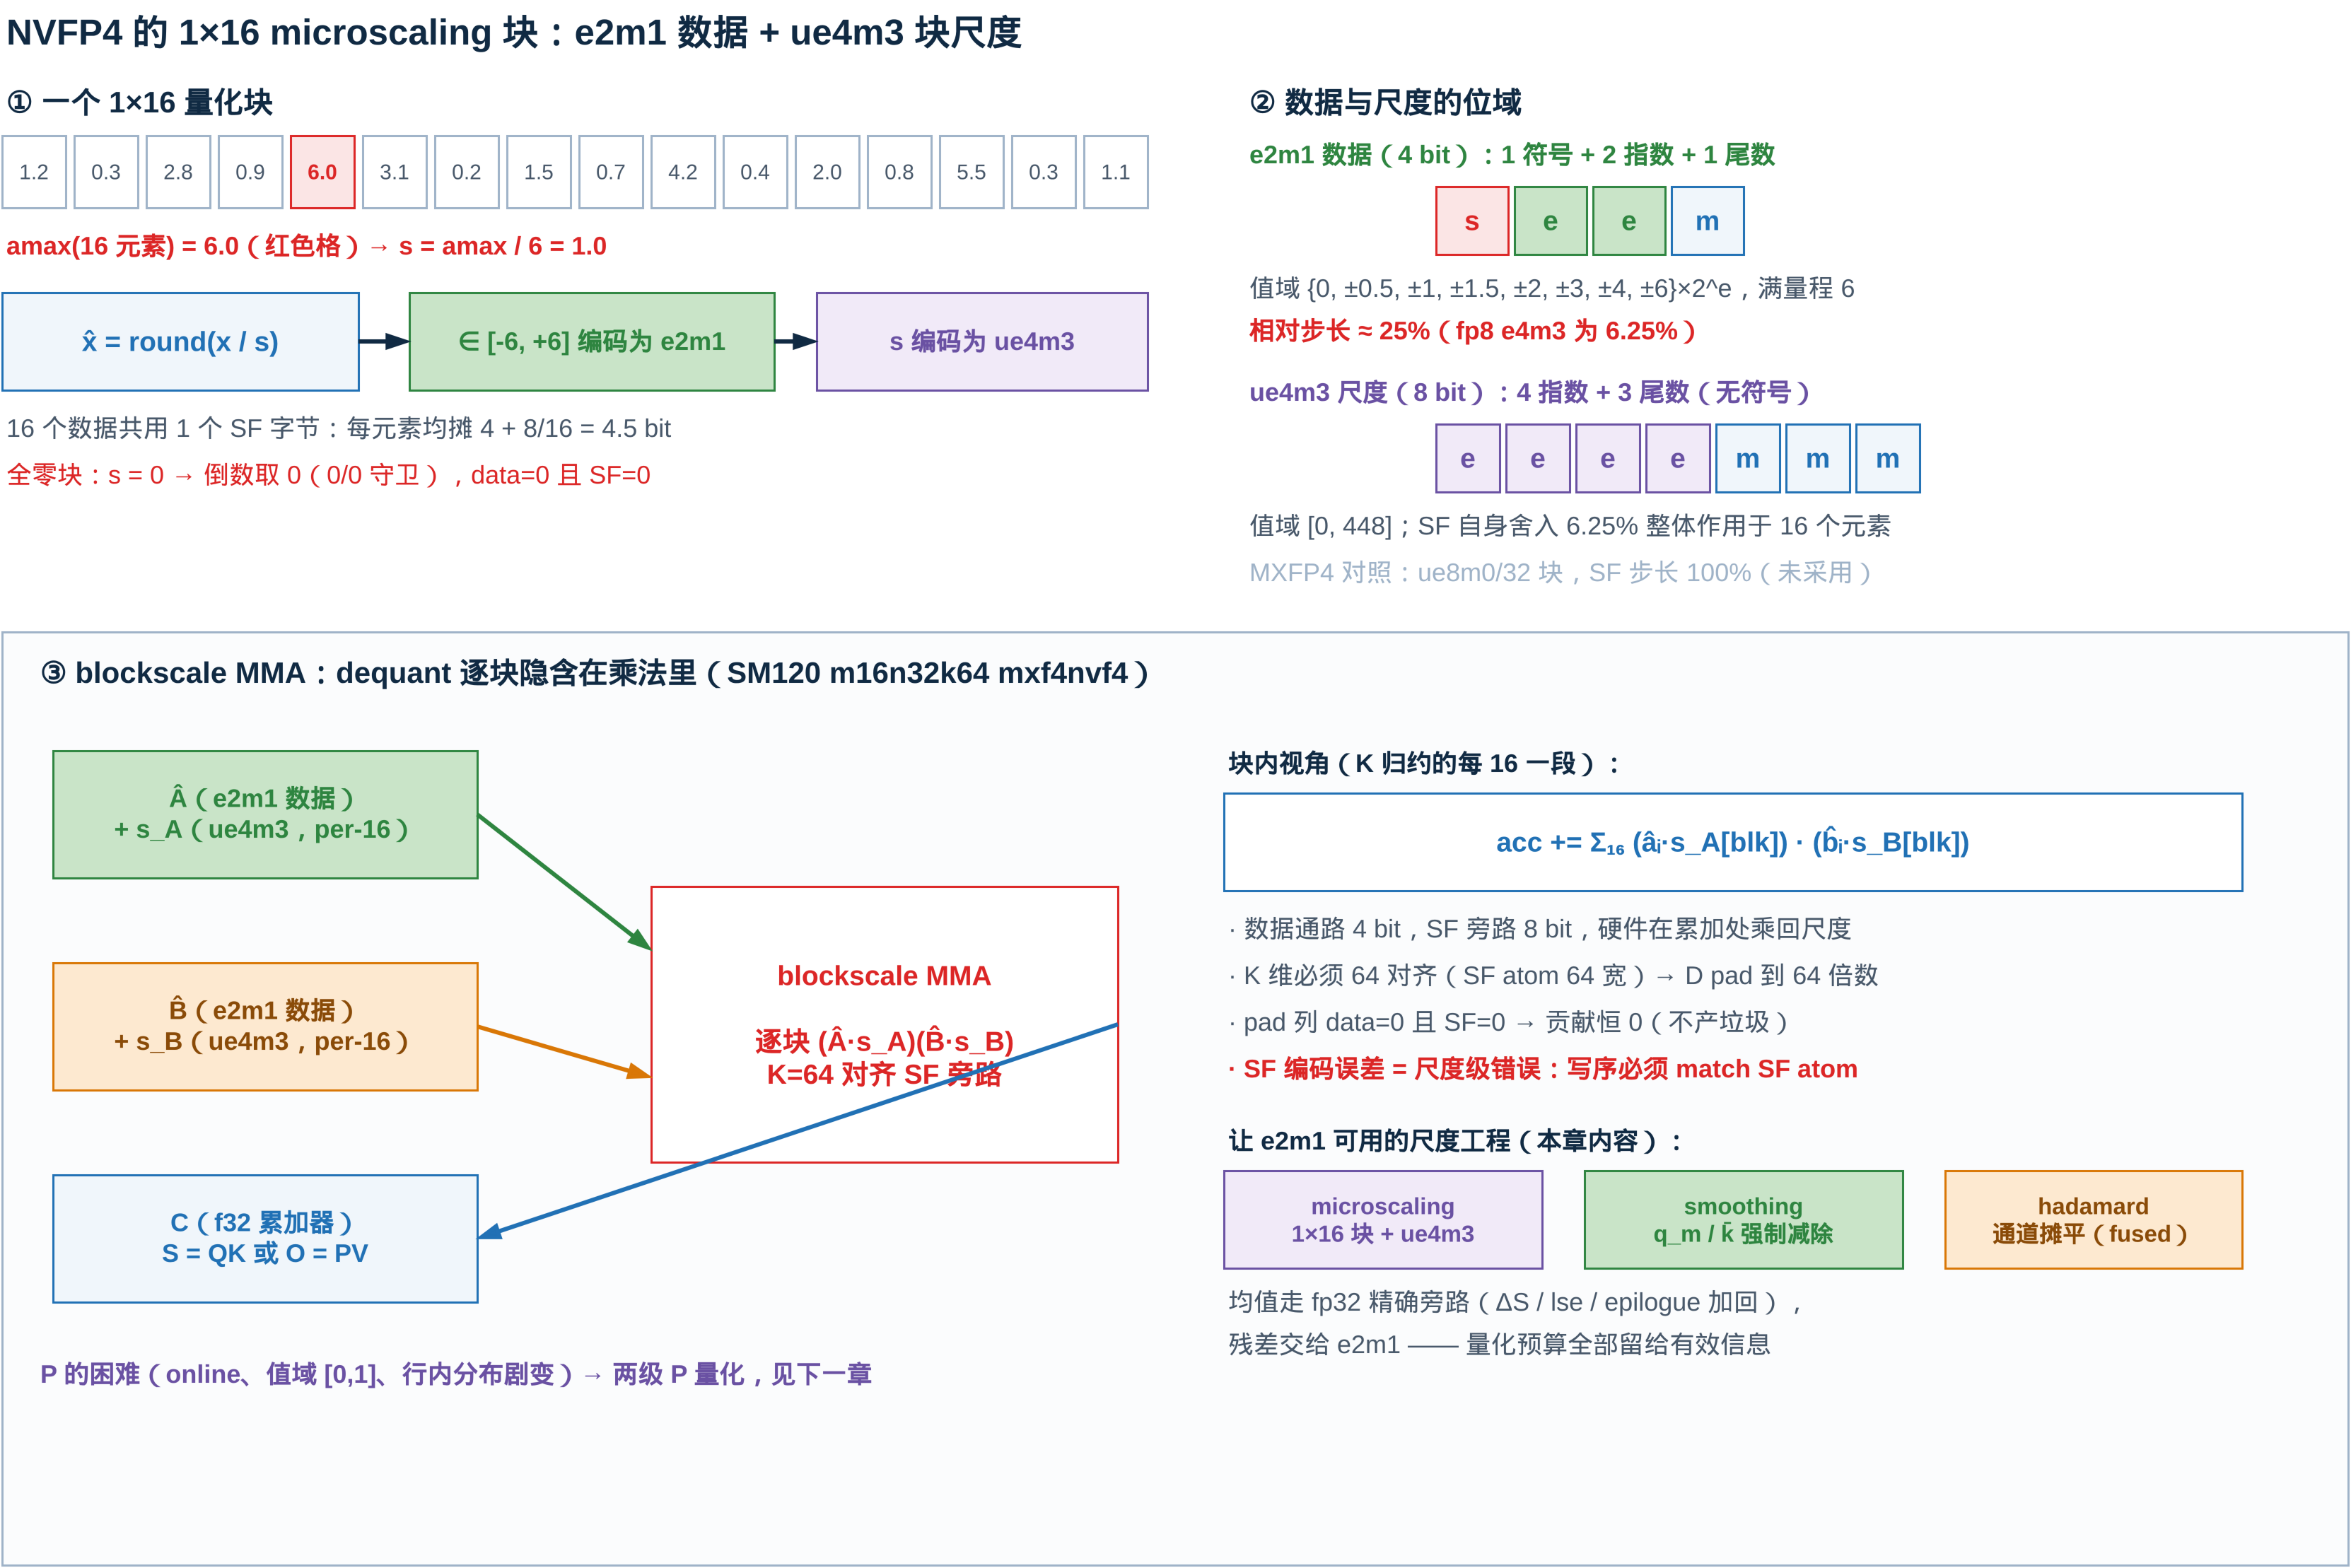
\includegraphics[width=0.98\textwidth]{figures/drawio/fig-31-1-nvfp4-block/fig-31-1-nvfp4-block.png}
  \begin{tikzpicture}
    \node[anchor=west, inner sep=0pt, align=left, font={\fontsize{7.4}{9.3}\selectfont \bfseries }] at (0.37,-0.354) {NVFP4 的 1$\times$16 microscaling 块：e2m1 数据 + ue4m3 块尺度};% w=16.940
    \node[anchor=west, inner sep=0pt, align=left, font={\fontsize{6.1}{7.7}\selectfont \bfseries }] at (0.37,-0.862) {(1) 一个 1$\times$16 量化块};% w=8.316
    \node[draw=gray!55, fill=none, line width=0.5pt, minimum width=0.46cm, minimum height=0.52cm, inner sep=1pt, align=center, text width=0.40cm, font={\fontsize{4.4}{5.5}\selectfont \color{black!65} }] at (0.601,-1.371) {1.2};
    \node[draw=gray!55, fill=none, line width=0.5pt, minimum width=0.46cm, minimum height=0.52cm, inner sep=1pt, align=center, text width=0.40cm, font={\fontsize{4.4}{5.5}\selectfont \color{black!65} }] at (1.124,-1.371) {0.3};
    \node[draw=gray!55, fill=none, line width=0.5pt, minimum width=0.46cm, minimum height=0.52cm, inner sep=1pt, align=center, text width=0.40cm, font={\fontsize{4.4}{5.5}\selectfont \color{black!65} }] at (1.648,-1.371) {2.8};
    \node[draw=gray!55, fill=none, line width=0.5pt, minimum width=0.46cm, minimum height=0.52cm, inner sep=1pt, align=center, text width=0.40cm, font={\fontsize{4.4}{5.5}\selectfont \color{black!65} }] at (2.171,-1.371) {0.9};
    \node[draw=tkRed, fill=tkFillRed, line width=0.5pt, minimum width=0.46cm, minimum height=0.52cm, inner sep=1pt, align=center, text width=0.40cm, font={\fontsize{4.4}{5.5}\selectfont \bfseries \color{tkRed} }] at (2.695,-1.371) {6.0};
    \node[draw=gray!55, fill=none, line width=0.5pt, minimum width=0.46cm, minimum height=0.52cm, inner sep=1pt, align=center, text width=0.40cm, font={\fontsize{4.4}{5.5}\selectfont \color{black!65} }] at (3.219,-1.371) {3.1};
    \node[draw=gray!55, fill=none, line width=0.5pt, minimum width=0.46cm, minimum height=0.52cm, inner sep=1pt, align=center, text width=0.40cm, font={\fontsize{4.4}{5.5}\selectfont \color{black!65} }] at (3.742,-1.371) {0.2};
    \node[draw=gray!55, fill=none, line width=0.5pt, minimum width=0.46cm, minimum height=0.52cm, inner sep=1pt, align=center, text width=0.40cm, font={\fontsize{4.4}{5.5}\selectfont \color{black!65} }] at (4.266,-1.371) {1.5};
    \node[draw=gray!55, fill=none, line width=0.5pt, minimum width=0.46cm, minimum height=0.52cm, inner sep=1pt, align=center, text width=0.40cm, font={\fontsize{4.4}{5.5}\selectfont \color{black!65} }] at (4.789,-1.371) {0.7};
    \node[draw=gray!55, fill=none, line width=0.5pt, minimum width=0.46cm, minimum height=0.52cm, inner sep=1pt, align=center, text width=0.40cm, font={\fontsize{4.4}{5.5}\selectfont \color{black!65} }] at (5.313,-1.371) {4.2};
    \node[draw=gray!55, fill=none, line width=0.5pt, minimum width=0.46cm, minimum height=0.52cm, inner sep=1pt, align=center, text width=0.40cm, font={\fontsize{4.4}{5.5}\selectfont \color{black!65} }] at (5.837,-1.371) {0.4};
    \node[draw=gray!55, fill=none, line width=0.5pt, minimum width=0.46cm, minimum height=0.52cm, inner sep=1pt, align=center, text width=0.40cm, font={\fontsize{4.4}{5.5}\selectfont \color{black!65} }] at (6.36,-1.371) {2.0};
    \node[draw=gray!55, fill=none, line width=0.5pt, minimum width=0.46cm, minimum height=0.52cm, inner sep=1pt, align=center, text width=0.40cm, font={\fontsize{4.4}{5.5}\selectfont \color{black!65} }] at (6.884,-1.371) {0.8};
    \node[draw=gray!55, fill=none, line width=0.5pt, minimum width=0.46cm, minimum height=0.52cm, inner sep=1pt, align=center, text width=0.40cm, font={\fontsize{4.4}{5.5}\selectfont \color{black!65} }] at (7.407,-1.371) {5.5};
    \node[draw=gray!55, fill=none, line width=0.5pt, minimum width=0.46cm, minimum height=0.52cm, inner sep=1pt, align=center, text width=0.40cm, font={\fontsize{4.4}{5.5}\selectfont \color{black!65} }] at (7.931,-1.371) {0.3};
    \node[draw=gray!55, fill=none, line width=0.5pt, minimum width=0.46cm, minimum height=0.52cm, inner sep=1pt, align=center, text width=0.40cm, font={\fontsize{4.4}{5.5}\selectfont \color{black!65} }] at (8.455,-1.371) {1.1};
    \node[anchor=west, inner sep=0pt, align=left, font={\fontsize{5.2}{6.6}\selectfont \bfseries \color{tkRed} }] at (0.37,-1.91) {amax(16 元素) = 6.0（红色格）$\to$ s = amax / 6 = 1.0};% w=8.393
    \node[draw=tkBlue, fill=tkFillBlue, line width=0.5pt, minimum width=2.59cm, minimum height=0.71cm, inner sep=1pt, align=center, text width=2.53cm, font={\fontsize{5.7}{7.1}\selectfont \bfseries \color{tkBlue} }] at (1.663,-2.603) {$\hat{x}$ = round(x / s)};
    \node[draw=tkGreen, fill=tkFillGreen, line width=0.5pt, minimum width=2.65cm, minimum height=0.71cm, inner sep=1pt, align=center, text width=2.59cm, font={\fontsize{5.2}{6.6}\selectfont \bfseries \color{tkGreen!70!black} }] at (4.651,-2.603) {$\in$ [-6, +6] 编码为 e2m1};
    \node[draw=tkPurple, fill=tkFillPurple, line width=0.5pt, minimum width=2.40cm, minimum height=0.71cm, inner sep=1pt, align=center, text width=2.34cm, font={\fontsize{5.2}{6.6}\selectfont \bfseries \color{tkPurple} }] at (7.484,-2.603) {s 编码为 ue4m3};
    \node[anchor=west, inner sep=0pt, align=left, font={\fontsize{5.2}{6.6}\selectfont \color{black!65} }] at (0.37,-3.234) {16 个数据共用 1 个 SF 字节：每元素均摊 4 + 8/16 = 4.5 bit};% w=8.393
    \node[anchor=west, inner sep=0pt, align=left, font={\fontsize{5.2}{6.6}\selectfont \color{tkRed} }] at (0.37,-3.573) {全零块：s = 0 $\to$ 倒数取 0（0/0 守卫），data=0 且 SF=0};% w=8.393
    \node[anchor=west, inner sep=0pt, align=left, font={\fontsize{6.1}{7.7}\selectfont \bfseries }] at (9.394,-0.862) {(2) 数据与尺度的位域};% w=8.008
    \node[anchor=west, inner sep=0pt, align=left, font={\fontsize{5.2}{6.6}\selectfont \bfseries \color{tkGreen!70!black} }] at (9.394,-1.247) {e2m1 数据（4 bit）：1 符号 + 2 指数 + 1 尾数};% w=8.008
    \node[draw=tkRed, fill=tkFillRed, line width=0.5pt, minimum width=0.52cm, minimum height=0.49cm, inner sep=1pt, align=center, text width=0.46cm, font={\fontsize{5.7}{7.1}\selectfont \bfseries \color{tkRed} }] at (11.042,-1.725) {s};
    \node[draw=tkGreen, fill=tkFillGreen, line width=0.5pt, minimum width=0.52cm, minimum height=0.49cm, inner sep=1pt, align=center, text width=0.46cm, font={\fontsize{5.7}{7.1}\selectfont \bfseries \color{tkGreen!70!black} }] at (11.612,-1.725) {e};
    \node[draw=tkGreen, fill=tkFillGreen, line width=0.5pt, minimum width=0.52cm, minimum height=0.49cm, inner sep=1pt, align=center, text width=0.46cm, font={\fontsize{5.7}{7.1}\selectfont \bfseries \color{tkGreen!70!black} }] at (12.181,-1.725) {e};
    \node[draw=tkBlue, fill=tkFillBlue, line width=0.5pt, minimum width=0.52cm, minimum height=0.49cm, inner sep=1pt, align=center, text width=0.46cm, font={\fontsize{5.7}{7.1}\selectfont \bfseries \color{tkBlue} }] at (12.751,-1.725) {m};
    \node[anchor=west, inner sep=0pt, align=left, font={\fontsize{5.2}{6.6}\selectfont \color{black!65} }] at (9.394,-2.218) {值域 $\{0,\pm0.5,\pm1,\pm1.5,\pm2,\pm3,\pm4,\pm6\}$，满量程 6};% w=8.008
    \node[anchor=west, inner sep=0pt, align=left, font={\fontsize{5.2}{6.6}\selectfont \bfseries \color{tkRed} }] at (9.394,-2.526) {正规数相对误差通用上界 $\approx$25\%（e4m3 为 6.25\%）};% w=8.008
    \node[anchor=west, inner sep=0pt, align=left, font={\fontsize{5.2}{6.6}\selectfont \bfseries \color{tkPurple} }] at (9.394,-2.972) {ue4m3 尺度（8 bit）：4 指数 + 3 尾数（无符号）};% w=8.008
    \node[draw=tkPurple, fill=tkFillPurple, line width=0.5pt, minimum width=0.46cm, minimum height=0.49cm, inner sep=1pt, align=center, text width=0.40cm, font={\fontsize{5.7}{7.1}\selectfont \bfseries \color{tkPurple} }] at (11.011,-3.45) {e};
    \node[draw=tkPurple, fill=tkFillPurple, line width=0.5pt, minimum width=0.46cm, minimum height=0.49cm, inner sep=1pt, align=center, text width=0.40cm, font={\fontsize{5.7}{7.1}\selectfont \bfseries \color{tkPurple} }] at (11.519,-3.45) {e};
    \node[draw=tkPurple, fill=tkFillPurple, line width=0.5pt, minimum width=0.46cm, minimum height=0.49cm, inner sep=1pt, align=center, text width=0.40cm, font={\fontsize{5.7}{7.1}\selectfont \bfseries \color{tkPurple} }] at (12.027,-3.45) {e};
    \node[draw=tkPurple, fill=tkFillPurple, line width=0.5pt, minimum width=0.46cm, minimum height=0.49cm, inner sep=1pt, align=center, text width=0.40cm, font={\fontsize{5.7}{7.1}\selectfont \bfseries \color{tkPurple} }] at (12.536,-3.45) {e};
    \node[draw=tkBlue, fill=tkFillBlue, line width=0.5pt, minimum width=0.46cm, minimum height=0.49cm, inner sep=1pt, align=center, text width=0.40cm, font={\fontsize{5.7}{7.1}\selectfont \bfseries \color{tkBlue} }] at (13.044,-3.45) {m};
    \node[draw=tkBlue, fill=tkFillBlue, line width=0.5pt, minimum width=0.46cm, minimum height=0.49cm, inner sep=1pt, align=center, text width=0.40cm, font={\fontsize{5.7}{7.1}\selectfont \bfseries \color{tkBlue} }] at (13.552,-3.45) {m};
    \node[draw=tkBlue, fill=tkFillBlue, line width=0.5pt, minimum width=0.46cm, minimum height=0.49cm, inner sep=1pt, align=center, text width=0.40cm, font={\fontsize{5.7}{7.1}\selectfont \bfseries \color{tkBlue} }] at (14.06,-3.45) {m};
    \node[anchor=west, inner sep=0pt, align=left, font={\fontsize{5.2}{6.6}\selectfont \color{black!65} }] at (9.394,-3.942) {值域 [0, 448]；SF 自身舍入 6.25\% 整体作用于 16 个元素};% w=8.008
    \node[anchor=west, inner sep=0pt, align=left, font={\fontsize{5.2}{6.6}\selectfont \color{black!45} }] at (9.394,-4.281) {MXFP4 对照：ue8m0/32 块，SF 步长 100\%（未采用）};% w=8.008
    \node[draw=gray!55, fill=black!2, line width=0.5pt, minimum width=17.03cm, minimum height=6.78cm, inner sep=1pt, align=center, text width=16.97cm, font={\fontsize{5.7}{7.1}\selectfont }] at (8.886,-8.1) {};
    \node[anchor=west, inner sep=0pt, align=left, font={\fontsize{6.1}{7.7}\selectfont \bfseries }] at (0.616,-5.005) {(3) blockscale MMA：dequant 逐块隐含在乘法里（SM120 m16n32k64 mxf4nvf4）};% w=16.478
    \node[draw=tkGreen, fill=tkFillGreen, line width=0.5pt, minimum width=3.08cm, minimum height=0.92cm, inner sep=1pt, align=center, text width=3.02cm, font={\fontsize{5.2}{6.6}\selectfont \bfseries \color{tkGreen!70!black} }] at (2.279,-6.037) {$\hat{A}$（e2m1 数据）\\+ s\_A（ue4m3，per-group (16)）};
    \node[draw=tkOrange, fill=tkFillOrange, line width=0.5pt, minimum width=3.08cm, minimum height=0.92cm, inner sep=1pt, align=center, text width=3.02cm, font={\fontsize{5.2}{6.6}\selectfont \bfseries \color{tkOrange!75!black} }] at (2.279,-7.577) {$\hat{B}$（e2m1 数据）\\+ s\_B（ue4m3，per-group (16)）};
    \node[draw=tkBlue, fill=tkFillBlue, line width=0.5pt, minimum width=3.08cm, minimum height=0.92cm, inner sep=1pt, align=center, text width=3.02cm, font={\fontsize{5.2}{6.6}\selectfont \bfseries \color{tkBlue} }] at (2.279,-9.117) {C（f32 累加器）\\S = QK 或 O = PV};
    \node[draw=tkRed, fill=none, line width=0.5pt, minimum width=3.39cm, minimum height=2.00cm, inner sep=1pt, align=center, text width=3.33cm, font={\fontsize{5.7}{7.1}\selectfont \bfseries \color{tkRed} }] at (6.776,-7.561) {blockscale MMA\\逐块 ($\hat{A}$$\cdot$s\_A)($\hat{B}$$\cdot$s\_B)\\K=64 对齐 SF 旁路};
    \node[anchor=west, inner sep=0pt, align=left, font={\fontsize{5.2}{6.6}\selectfont \bfseries }] at (9.24,-5.667) {块内视角（K 归约的每 16 一段）：};% w=7.700
    \node[draw=tkBlue, fill=none, line width=0.5pt, minimum width=7.39cm, minimum height=0.71cm, inner sep=1pt, align=center, text width=7.33cm, font={\fontsize{5.7}{7.1}\selectfont \bfseries \color{tkBlue} }] at (12.936,-6.237) {acc += $\Sigma$$_1$$_6$ ($\hat{a}$$_i$$\cdot$s\_A[blk]) $\cdot$ ($\hat{b}$$_i$$\cdot$s\_B[blk])};
    \node[anchor=west, inner sep=0pt, align=left, font={\fontsize{5.2}{6.6}\selectfont \color{black!65} }] at (9.24,-6.868) {$\cdot$ 数据通路 4 bit，SF 旁路 8 bit，硬件在累加处乘回尺度};% w=7.700
    \node[anchor=west, inner sep=0pt, align=left, font={\fontsize{5.2}{6.6}\selectfont \color{black!65} }] at (9.24,-7.207) {$\cdot$ K 维必须 64 对齐（SF atom 64 宽）$\to$ D pad 到 64 倍数};% w=7.700
    \node[anchor=west, inner sep=0pt, align=left, font={\fontsize{5.2}{6.6}\selectfont \color{black!65} }] at (9.24,-7.546) {$\cdot$ pad 列 data=0 且 SF=0 $\to$ 贡献恒 0（不污染结果）};% w=7.700
    \node[anchor=west, inner sep=0pt, align=left, font={\fontsize{5.2}{6.6}\selectfont \bfseries \color{tkRed} }] at (9.24,-7.885) {$\cdot$ SF 编码误差 = 尺度级错误：写序必须 match SF atom};% w=7.700
    \node[anchor=west, inner sep=0pt, align=left, font={\fontsize{5.2}{6.6}\selectfont \bfseries }] at (9.24,-8.408) {让 e2m1 可用的尺度处理（本章内容）：};% w=7.700
    \node[draw=tkPurple, fill=tkFillPurple, line width=0.5pt, minimum width=2.31cm, minimum height=0.71cm, inner sep=1pt, align=center, text width=2.25cm, font={\fontsize{4.8}{6.0}\selectfont \bfseries \color{tkPurple} }] at (10.395,-8.978) {microscaling\\1$\times$16 块 + ue4m3};
    \node[draw=tkGreen, fill=tkFillGreen, line width=0.5pt, minimum width=2.31cm, minimum height=0.71cm, inner sep=1pt, align=center, text width=2.25cm, font={\fontsize{4.8}{6.0}\selectfont \bfseries \color{tkGreen!70!black} }] at (13.013,-8.978) {smoothing\\q\_m / $\bar{k}$ 强制减除};
    \node[draw=tkOrange, fill=tkFillOrange, line width=0.5pt, minimum width=2.16cm, minimum height=0.71cm, inner sep=1pt, align=center, text width=2.09cm, font={\fontsize{4.8}{6.0}\selectfont \bfseries \color{tkOrange!75!black} }] at (15.554,-8.978) {hadamard\\通道摊平（fused）};
    \node[anchor=west, inner sep=0pt, align=left, font={\fontsize{5.2}{6.6}\selectfont \color{black!65} }] at (9.24,-9.579) {均值走 fp32 精确旁路（$\Delta$S / lse / epilogue 加回），};% w=7.700
    \node[anchor=west, inner sep=0pt, align=left, font={\fontsize{5.2}{6.6}\selectfont \color{black!65} }] at (9.24,-9.887) {残差交给 e2m1 ------ 量化预算全部留给有效信息};% w=7.700
    \node[anchor=west, inner sep=0pt, align=left, font={\fontsize{5.2}{6.6}\selectfont \bfseries \color{tkPurple} }] at (0.616,-10.102) {P 的困难（online、值域 [0,1]、行内分布剧变）$\to$ 两级 P 量化，见下一章};% w=8.316
    \draw[black!75, line width=0.8pt, -{Stealth[length=2.2pt,width=1.8pt]}] (2.957,-2.603) -- (3.326,-2.603);
    \draw[black!75, line width=0.8pt, -{Stealth[length=2.2pt,width=1.8pt]}] (5.975,-2.603) -- (6.283,-2.603);
    \draw[tkGreen, line width=0.8pt, -{Stealth[length=2.2pt,width=1.8pt]}] (3.819,-6.037) -- (5.082,-7.022);
    \draw[tkOrange, line width=0.8pt, -{Stealth[length=2.2pt,width=1.8pt]}] (3.819,-7.577) -- (5.082,-7.946);
    \draw[tkBlue, line width=0.8pt, -{Stealth[length=2.2pt,width=1.8pt]}] (8.47,-7.561) -- (3.819,-9.117);
  \end{tikzpicture}
  \caption{NVFP4 的 $1\times16$ microscaling 块：e2m1 数据位域与
  ue4m3 块尺度。$s_{block}=\mathrm{amax}/6$ 除进数据、乘回在
  blockscale MMA 内逐块完成。}
  \label{fig:31-1}
\end{figure}

\begin{figure}[htbp]
  \centering
  % was: 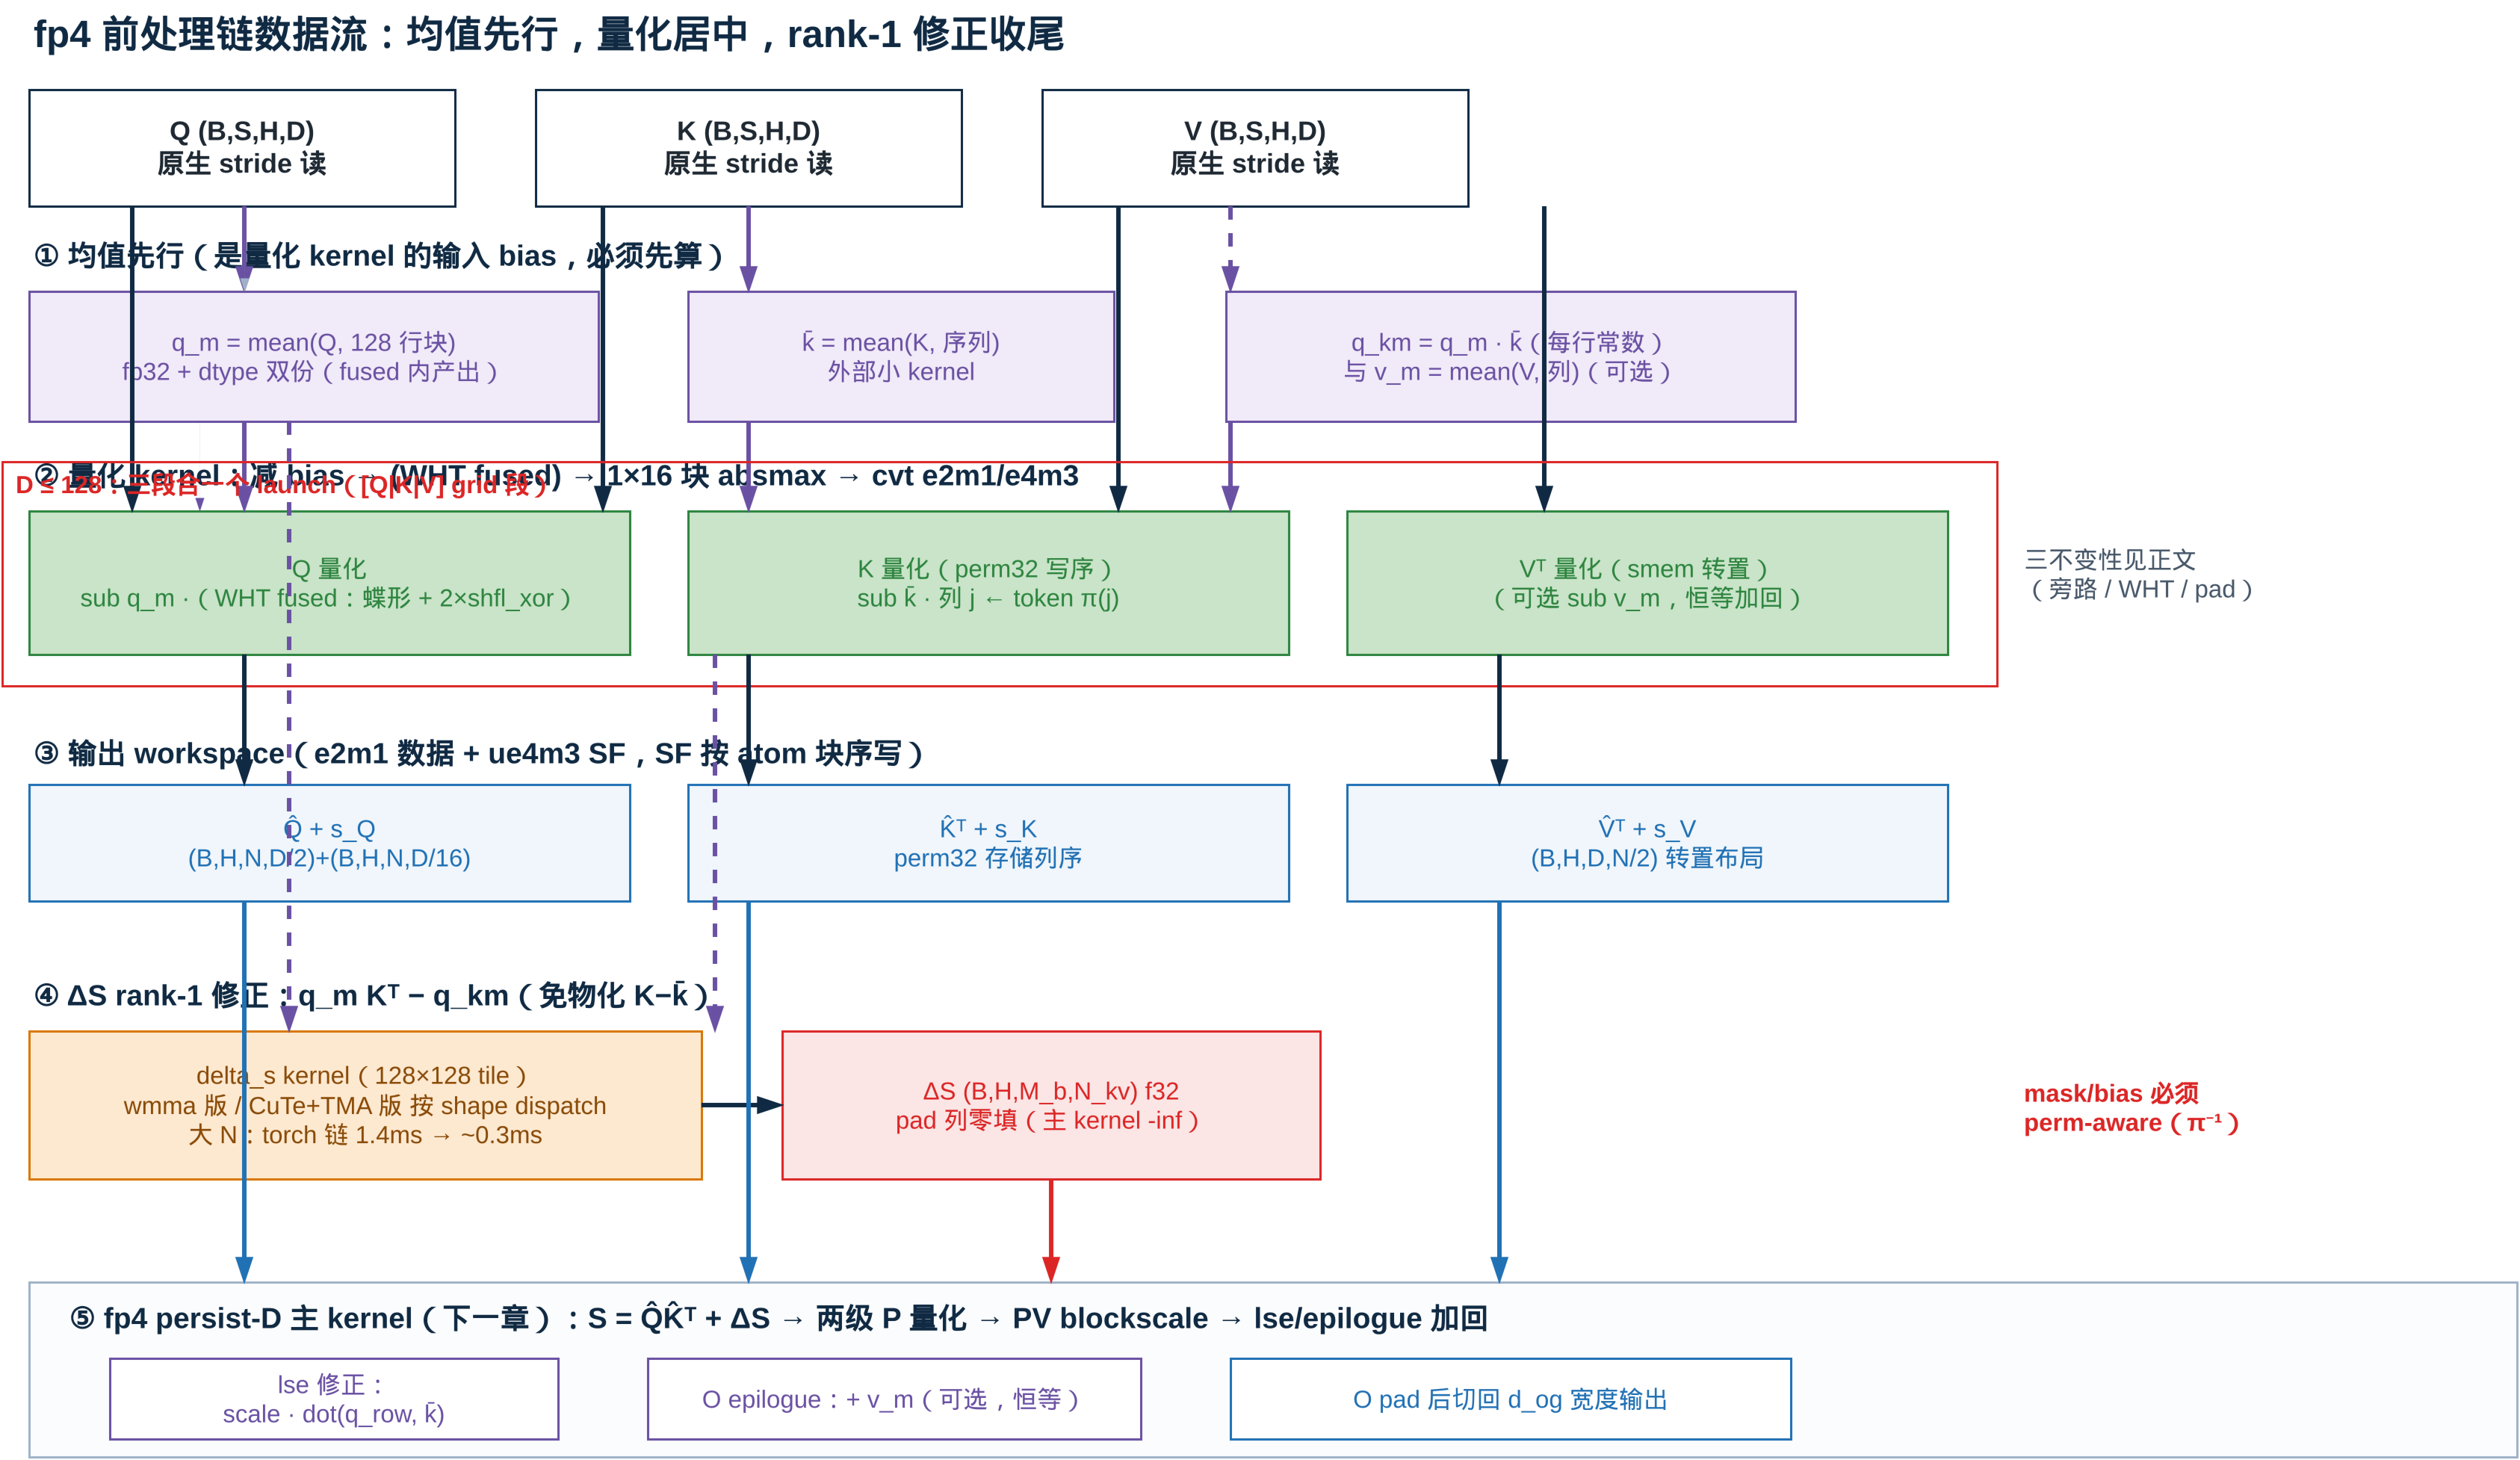
\includegraphics[width=0.98\textwidth]{figures/drawio/fig-31-2-fp4-pipeline/fig-31-2-fp4-pipeline.png}
  \begin{tikzpicture}
    \node[anchor=west, fill=white, inner sep=1pt, align=left, font={\fontsize{7.4}{9.3}\selectfont \bfseries }] at (0.37,-0.354) {fp4 前处理链数据流：均值先行，量化居中，rank-1 修正收尾};% w=17.094
    \node[draw=black!75, fill=none, line width=0.5pt, minimum width=2.93cm, minimum height=0.80cm, inner sep=1pt, align=center, text width=2.86cm, font={\fontsize{5.2}{6.6}\selectfont \bfseries }] at (1.833,-1.14) {Q (B,S,H,D)\\原生 stride 读};
    \node[draw=black!75, fill=none, line width=0.5pt, minimum width=2.93cm, minimum height=0.80cm, inner sep=1pt, align=center, text width=2.86cm, font={\fontsize{5.2}{6.6}\selectfont \bfseries }] at (5.313,-1.14) {K (B,S,H,D)\\原生 stride 读};
    \node[draw=black!75, fill=none, line width=0.5pt, minimum width=2.93cm, minimum height=0.80cm, inner sep=1pt, align=center, text width=2.86cm, font={\fontsize{5.2}{6.6}\selectfont \bfseries }] at (8.793,-1.14) {V (B,S,H,D)\\原生 stride 读};
    \node[draw=tkPurple, fill=tkFillPurple, line width=0.5pt, minimum width=3.91cm, minimum height=0.89cm, inner sep=1pt, align=center, text width=3.85cm, font={\fontsize{4.8}{6.0}\selectfont \color{tkPurple} }] at (2.325,-2.572) {q\_m = mean(Q, 128 行块)\\fp32 + dtype 双份（fused 内产出）};
    \node[draw=tkPurple, fill=tkFillPurple, line width=0.5pt, minimum width=2.93cm, minimum height=0.89cm, inner sep=1pt, align=center, text width=2.86cm, font={\fontsize{4.8}{6.0}\selectfont \color{tkPurple} }] at (6.36,-2.572) {$\bar{k}$ = mean(K, 序列)\\外部小 kernel};
    \node[draw=tkPurple, fill=tkFillPurple, line width=0.5pt, minimum width=3.91cm, minimum height=0.89cm, inner sep=1pt, align=center, text width=3.85cm, font={\fontsize{4.8}{6.0}\selectfont \color{tkPurple} }] at (10.549,-2.572) {q\_km = q\_m $\cdot$ $\bar{k}$（每行常数）\\与 v\_m = mean(V, 列)（可选）};
    \node[draw=tkGreen, fill=tkFillGreen, line width=0.5pt, minimum width=4.13cm, minimum height=0.99cm, inner sep=1pt, align=center, text width=4.07cm, font={\fontsize{4.8}{6.0}\selectfont \color{tkGreen!70!black} }] at (2.433,-4.127) {Q 量化\\sub q\_m $\cdot$（WHT fused：蝶形 + 2$\times$shfl\_xor）};
    \node[draw=tkGreen, fill=tkFillGreen, line width=0.5pt, minimum width=4.13cm, minimum height=0.99cm, inner sep=1pt, align=center, text width=4.07cm, font={\fontsize{4.8}{6.0}\selectfont \color{tkGreen!70!black} }] at (6.961,-4.127) {K 量化（perm32 写序）\\sub $\bar{k}$ $\cdot$ 列 j $\leftarrow$ token $\pi$(j)};
    \node[draw=tkGreen, fill=tkFillGreen, line width=0.5pt, minimum width=4.13cm, minimum height=0.99cm, inner sep=1pt, align=center, text width=4.07cm, font={\fontsize{4.8}{6.0}\selectfont \color{tkGreen!70!black} }] at (11.488,-4.127) {V$^{\top}$ 量化（smem 转置）\\（可选 sub v\_m，恒等加回）};
    \node[draw=tkRed, fill=none, line width=0.5pt, minimum width=13.71cm, minimum height=1.20cm, inner sep=1pt, align=center, text width=13.64cm, font={\fontsize{5.7}{7.1}\selectfont }] at (7.038,-4.150) {};
    \node[draw=tkBlue, fill=tkFillBlue, line width=0.5pt, minimum width=4.13cm, minimum height=0.80cm, inner sep=1pt, align=center, text width=4.07cm, font={\fontsize{4.8}{6.0}\selectfont \color{tkBlue} }] at (2.433,-5.914) {$\hat{Q}$ + s\_Q\\(B,H,N,D/2)+(B,H,N,D/16)};
    \node[draw=tkBlue, fill=tkFillBlue, line width=0.5pt, minimum width=4.13cm, minimum height=0.80cm, inner sep=1pt, align=center, text width=4.07cm, font={\fontsize{4.8}{6.0}\selectfont \color{tkBlue} }] at (6.961,-5.914) {$\hat{K}$$^{\top}$ + s\_K\\perm32 存储列序};
    \node[draw=tkBlue, fill=tkFillBlue, line width=0.5pt, minimum width=4.13cm, minimum height=0.80cm, inner sep=1pt, align=center, text width=4.07cm, font={\fontsize{4.8}{6.0}\selectfont \color{tkBlue} }] at (11.488,-5.914) {$\hat{V}$$^{\top}$ + s\_V\\(B,H,D,N/2) 转置布局};
    \node[draw=tkOrange, fill=tkFillOrange, line width=0.5pt, minimum width=4.62cm, minimum height=1.02cm, inner sep=1pt, align=center, text width=4.56cm, font={\fontsize{4.8}{6.0}\selectfont \color{tkOrange!75!black} }] at (2.68,-7.715) {delta\_s kernel（128$\times$128 tile）\\wmma 版 / CuTe+TMA 版 按 shape dispatch\\大 N：torch 链 1.4ms $\to$ \textasciitilde{}0.3ms};
    \node[draw=tkRed, fill=tkFillRed, line width=0.5pt, minimum width=3.70cm, minimum height=1.02cm, inner sep=1pt, align=center, text width=3.63cm, font={\fontsize{4.8}{6.0}\selectfont \color{tkRed} }] at (7.392,-7.715) {$\Delta$S (B,H,M\_b,N\_kv) f32\\pad 列零填（主 kernel -inf）};
    \node[draw=gray!55, fill=black!2, line width=0.5pt, minimum width=17.09cm, minimum height=1.20cm, inner sep=1pt, align=center, text width=17.03cm, font={\fontsize{5.7}{7.1}\selectfont }] at (8.917,-9.533) {};
    \node[draw=tkPurple, fill=none, line width=0.5pt, minimum width=3.08cm, minimum height=0.55cm, inner sep=1pt, align=center, text width=3.02cm, font={\fontsize{4.8}{6.0}\selectfont \color{tkPurple} }] at (2.464,-9.733) {lse 修正：\\scale $\cdot$ dot(q\_row, $\bar{k}$)};
    \node[draw=tkPurple, fill=none, line width=0.5pt, minimum width=3.39cm, minimum height=0.55cm, inner sep=1pt, align=center, text width=3.33cm, font={\fontsize{4.8}{6.0}\selectfont \color{tkPurple} }] at (6.314,-9.733) {O epilogue：+ v\_m（可选，恒等）};
    \node[draw=tkBlue, fill=none, line width=0.5pt, minimum width=3.85cm, minimum height=0.55cm, inner sep=1pt, align=center, text width=3.79cm, font={\fontsize{4.8}{6.0}\selectfont \color{tkBlue} }] at (10.549,-9.733) {O pad 后切回 d\_og 宽度输出};
    \node[anchor=west, inner sep=0pt, align=left, font={\fontsize{4.8}{6.0}\selectfont \color{black!65} }] at (14.045,-4.066) {三不变性见正文\\（旁路 / WHT / pad）};% w=3.388
    \node[anchor=west, inner sep=0pt, align=left, font={\fontsize{4.8}{6.0}\selectfont \bfseries \color{tkRed} }] at (14.045,-7.731) {mask/bias 必须\\perm-aware（$\pi$）};% w=3.388
    \draw[tkPurple, line width=0.8pt, -{Stealth[length=2.2pt,width=1.8pt]}] (1.848,-1.54) -- (1.848,-2.125);
    \draw[tkPurple, line width=0.8pt, -{Stealth[length=2.2pt,width=1.8pt]}] (5.313,-1.54) -- (5.313,-2.125);
    \draw[tkPurple, line width=0.8pt, dashed, -{Stealth[length=2.2pt,width=1.8pt]}] (8.624,-1.54) -- (8.624,-2.125);
    \draw[tkPurple, line width=0.8pt, -{Stealth[length=2.2pt,width=1.8pt]}] (1.848,-3.018) -- (1.848,-3.634);
    \draw[tkPurple, line width=0.8pt, -{Stealth[length=2.2pt,width=1.8pt]}] (5.313,-3.018) -- (5.313,-3.634);
    \draw[tkPurple, line width=0.8pt, -{Stealth[length=2.2pt,width=1.8pt]}] (8.624,-3.018) -- (8.624,-3.634);
    \draw[gray!55, line width=0.5pt, -{Stealth[length=2.2pt,width=1.8pt]}] (1.848,-1.54) -- (1.848,-2.125);
    \draw[black!75, line width=0.8pt, -{Stealth[length=2.2pt,width=1.8pt]}] (1.078,-1.54) -- (1.078,-3.634);
    \draw[black!75, line width=0.8pt, -{Stealth[length=2.2pt,width=1.8pt]}] (4.312,-1.54) -- (4.312,-3.634);
    \draw[black!75, line width=0.8pt, -{Stealth[length=2.2pt,width=1.8pt]}] (7.854,-1.54) -- (7.854,-3.634);
    \draw[black!75, line width=0.8pt, -{Stealth[length=2.2pt,width=1.8pt]}] (10.78,-1.54) -- (10.78,-3.634);
    \draw[black!75, line width=0.8pt, -{Stealth[length=2.2pt,width=1.8pt]}] (1.848,-4.62) -- (1.848,-5.513);
    \draw[black!75, line width=0.8pt, -{Stealth[length=2.2pt,width=1.8pt]}] (5.313,-4.62) -- (5.313,-5.513);
    \draw[black!75, line width=0.8pt, -{Stealth[length=2.2pt,width=1.8pt]}] (10.472,-4.62) -- (10.472,-5.513);
    \draw[black!75, line width=0.8pt, -{Stealth[length=2.2pt,width=1.8pt]}] (4.99,-7.715) -- (5.544,-7.715);
    \draw[tkPurple, line width=0.5pt, -{Stealth[length=2.2pt,width=1.8pt]}] (1.54,-3.018) -- (1.54,-3.634);
    \draw[tkPurple, line width=0.8pt, dashed, -{Stealth[length=2.2pt,width=1.8pt]}] (2.156,-3.018) -- (2.156,-4.558) -- (2.156,-7.207);
    \draw[tkPurple, line width=0.8pt, dashed, -{Stealth[length=2.2pt,width=1.8pt]}] (5.082,-4.62) -- (5.082,-6.314) -- (5.082,-7.207);
    \draw[tkBlue, line width=0.8pt, -{Stealth[length=2.2pt,width=1.8pt]}] (1.848,-6.314) -- (1.848,-8.932);
    \draw[tkBlue, line width=0.8pt, -{Stealth[length=2.2pt,width=1.8pt]}] (5.313,-6.314) -- (5.313,-8.932);
    \draw[tkBlue, line width=0.8pt, -{Stealth[length=2.2pt,width=1.8pt]}] (10.472,-6.314) -- (10.472,-8.932);
    \draw[tkRed, line width=0.8pt, -{Stealth[length=2.2pt,width=1.8pt]}] (7.392,-8.224) -- (7.392,-8.932);
    \node[anchor=west, fill=white, inner sep=1pt, align=left, font={\fontsize{5.7}{7.1}\selectfont \bfseries }] at (0.37,-1.879) {(1) 均值先行（是量化 kernel 的输入 bias，必须先算）};% w=17.094
    \node[anchor=west, fill=white, inner sep=1pt, align=left, font={\fontsize{5.7}{7.1}\selectfont \bfseries }] at (0.37,-3.388) {(2) 量化 kernel：减 bias $\to$ (WHT fused) $\to$ 1$\times$16 块 absmax $\to$ cvt e2m1/e4m3};% w=17.094
    \node[anchor=west, fill=white, inner sep=1pt, align=left, font={\fontsize{4.8}{6.0}\selectfont \bfseries \color{tkRed} }] at (0.246,-3.049) {D $\leq$ 128：三段合一个 launch（[Q|K|V] grid 段）};% w=6.160
    \node[anchor=west, fill=white, inner sep=1pt, align=left, font={\fontsize{5.7}{7.1}\selectfont \bfseries }] at (0.37,-5.298) {(3) 输出 workspace（e2m1 数据 + ue4m3 SF，SF 按 atom 块序写）};% w=17.094
    \node[anchor=west, fill=white, inner sep=1pt, align=left, font={\fontsize{5.7}{7.1}\selectfont \bfseries }] at (0.37,-6.961) {(4) $\Delta$S rank-1 修正：q\_m K$^{\top}$ $-$ q\_km（免物化 K$-$$\bar{k}$）};% w=17.094
    \node[anchor=west, fill=white, inner sep=1pt, align=left, font={\fontsize{5.7}{7.1}\selectfont \bfseries }] at (0.616,-9.178) {(5) fp4 persist-D 主 kernel（下一章）：S = $\hat{Q}$$\hat{K}$$^{\top}$ + $\Delta$S $\to$ 两级 P 量化 $\to$ PV blockscale $\to$ lse/epilogue 加回};% w=16.478
  \end{tikzpicture}
  \caption{fp4 前处理链数据流（$D\le128$ 走 fused 单 launch 路径）：
  $\bar k$/$q_m$ 均值先行的原因是它们是量化 kernel 的输入 bias；
  hadamard 下 $q_m^{rot}$ 在 fused kernel 内同时产出。}
  \label{fig:31-2}
\end{figure}

\begin{figure}[htbp]
  \centering
  % was: 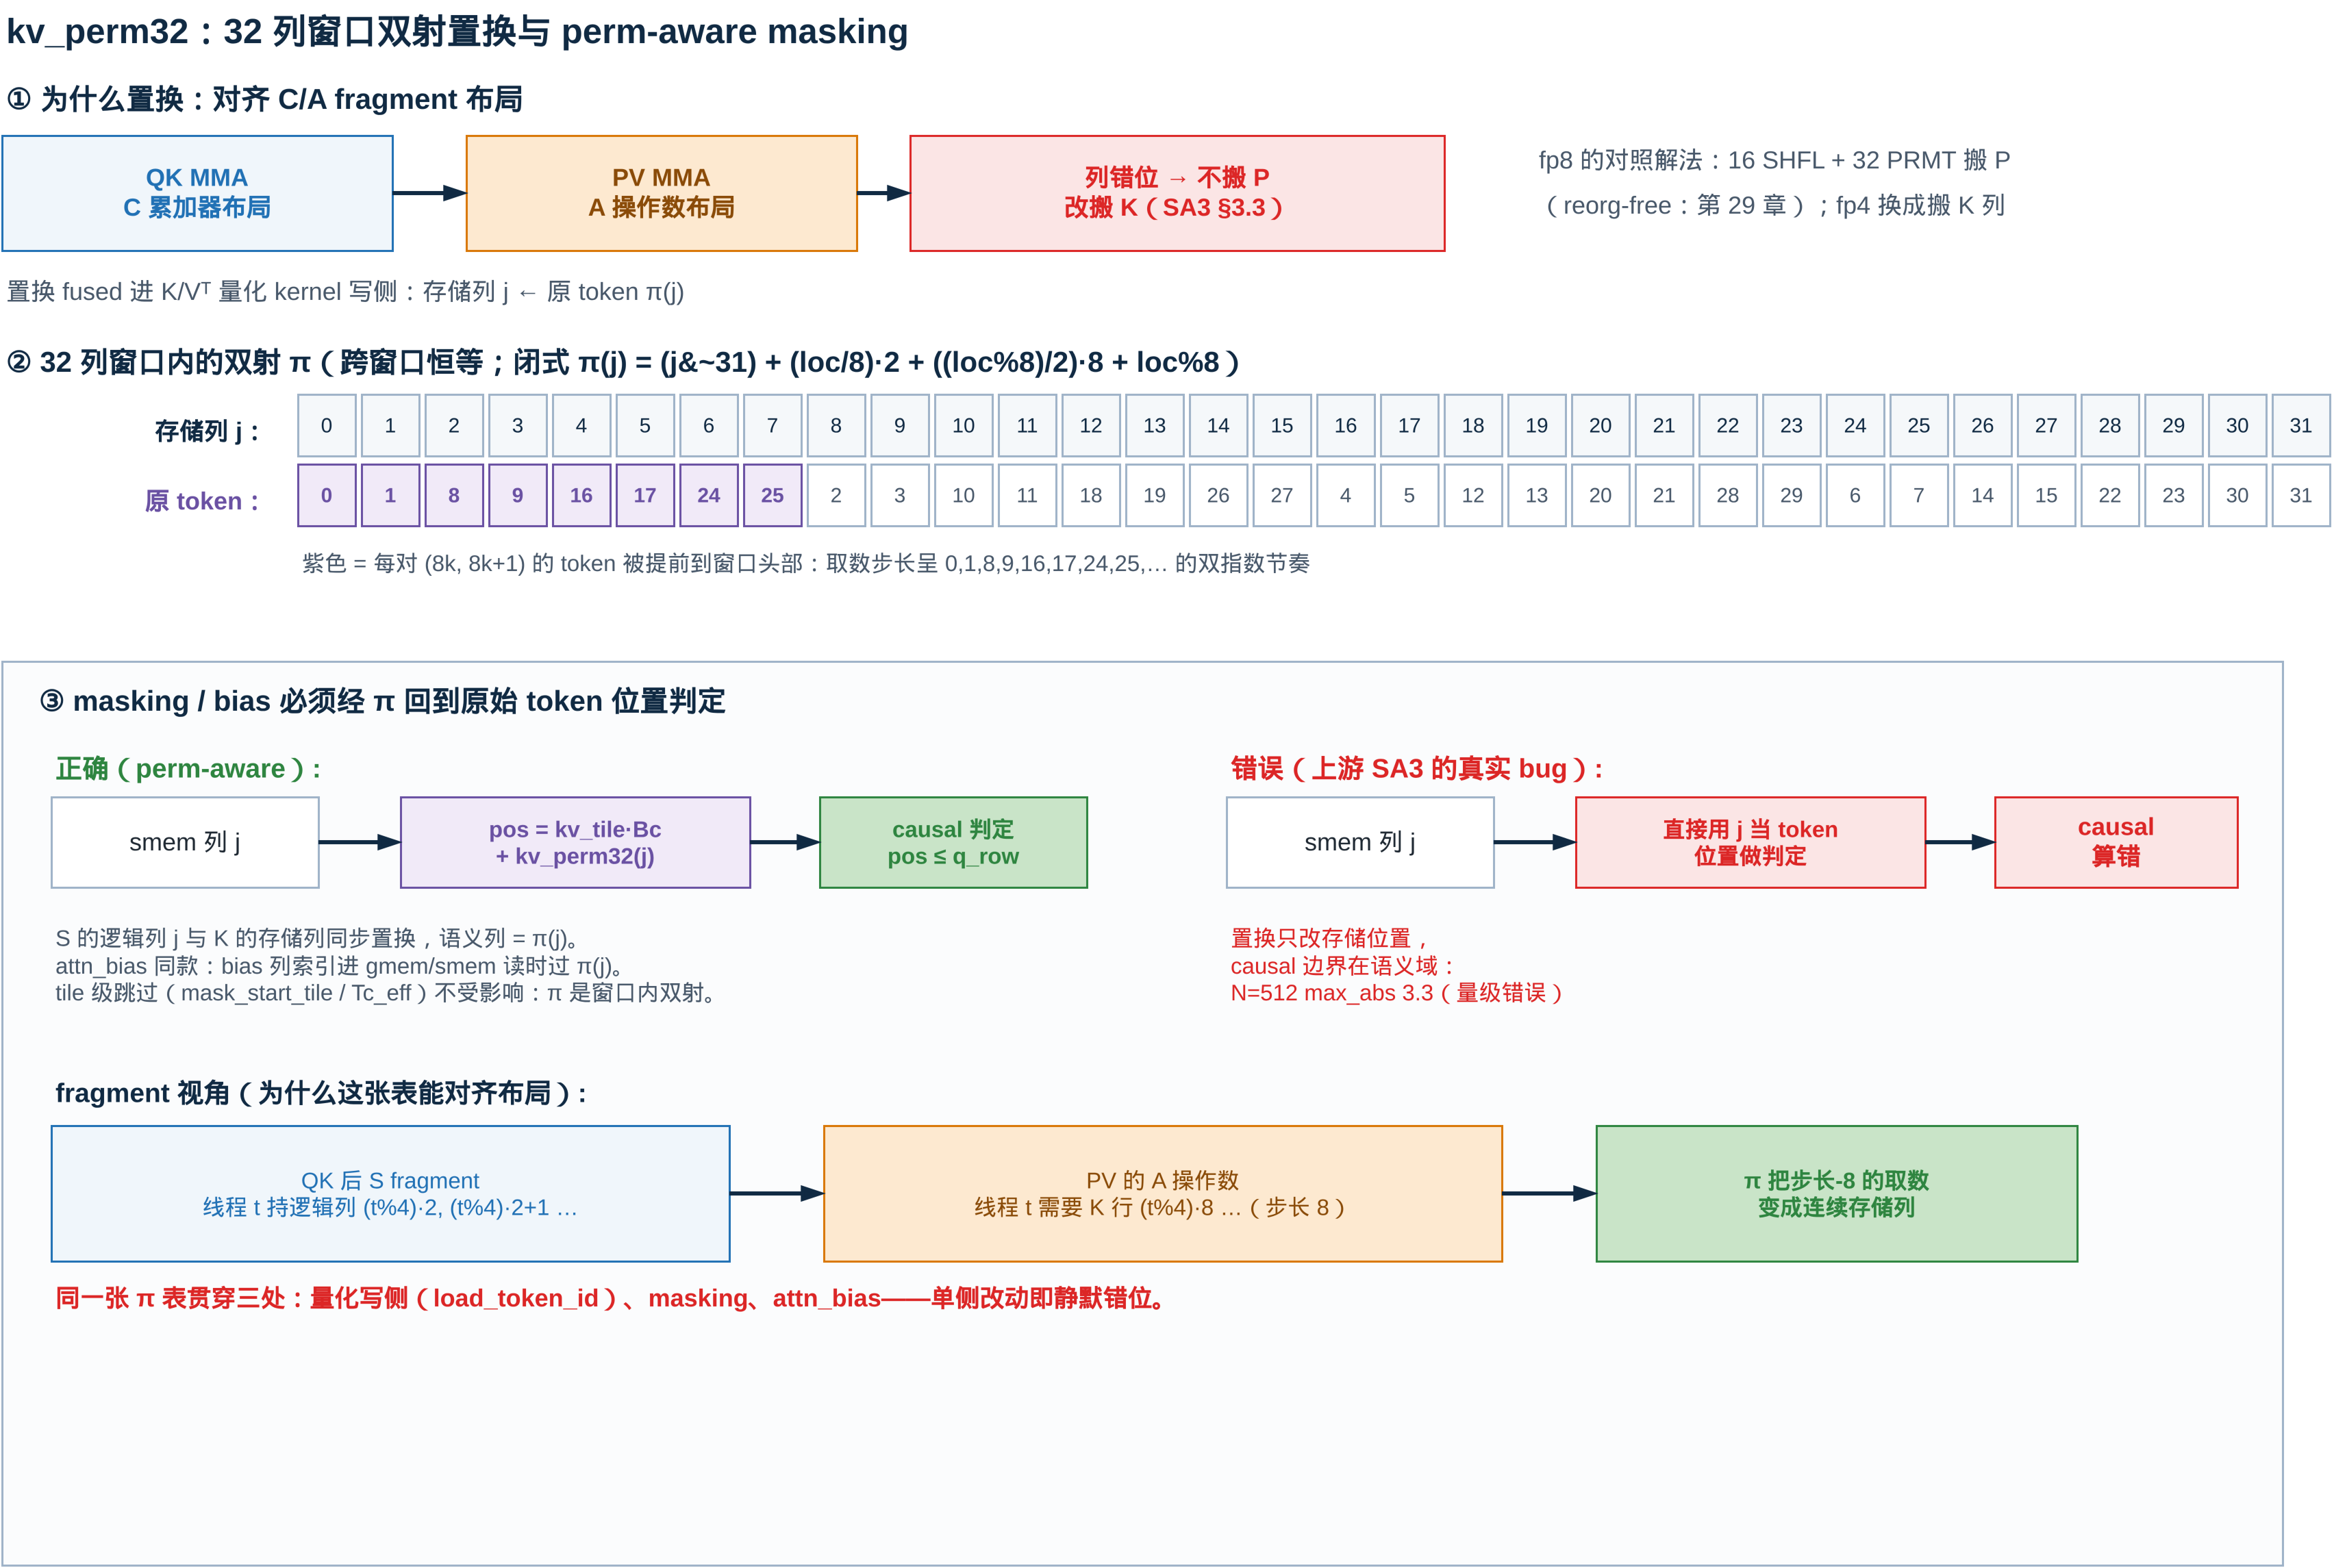
\includegraphics[width=0.98\textwidth]{figures/drawio/fig-31-3-kv-perm32/fig-31-3-kv-perm32.png}
  \begin{tikzpicture}
    \node[anchor=west, inner sep=0pt, align=left, font={\fontsize{7.4}{9.3}\selectfont \bfseries }] at (0.37,-0.354) {kv\_perm32：32 列窗口双射置换与 perm-aware masking};% w=17.094
    \node[anchor=west, inner sep=0pt, align=left, font={\fontsize{6.1}{7.7}\selectfont \bfseries }] at (0.37,-0.862) {(1) 为什么置换：对齐 C/A fragment 布局};% w=10.780
    \node[draw=tkBlue, fill=tkFillBlue, line width=0.5pt, minimum width=2.93cm, minimum height=0.86cm, inner sep=1pt, align=center, text width=2.86cm, font={\fontsize{5.2}{6.6}\selectfont \bfseries \color{tkBlue} }] at (1.833,-1.571) {QK MMA\\C 累加器布局};
    \node[draw=tkOrange, fill=tkFillOrange, line width=0.5pt, minimum width=2.93cm, minimum height=0.86cm, inner sep=1pt, align=center, text width=2.86cm, font={\fontsize{5.2}{6.6}\selectfont \bfseries \color{tkOrange!75!black} }] at (5.313,-1.571) {PV MMA\\A 操作数布局};
    \node[draw=tkRed, fill=tkFillRed, line width=0.5pt, minimum width=4.00cm, minimum height=0.86cm, inner sep=1pt, align=center, text width=3.94cm, font={\fontsize{5.2}{6.6}\selectfont \bfseries \color{tkRed} }] at (9.178,-1.571) {列错位 $\to$ 不搬 P\\改搬 K（SA3 \S{}3.3）};
    \node[anchor=west, inner sep=0pt, align=left, font={\fontsize{5.2}{6.6}\selectfont \color{black!65} }] at (11.858,-1.324) {fp8 的对照解法：16 SHFL + 32 PRMT 搬 P};% w=5.544
    \node[anchor=west, inner sep=0pt, align=left, font={\fontsize{5.2}{6.6}\selectfont \color{black!65} }] at (11.858,-1.663) {（reorg-free：第 \ref{ch:29} 章）；fp4 换成搬 K 列};% w=5.544
    \node[anchor=west, inner sep=0pt, align=left, font={\fontsize{5.2}{6.6}\selectfont \color{black!65} }] at (0.37,-2.31) {置换只 fused 进 K 量化 kernel 写侧：存储列 j $\leftarrow$ 原 token $\pi$(j)；$V^{\top}$ 保持自然序};% w=10.780
    \node[anchor=west, inner sep=0pt, align=left, font={\fontsize{6.1}{7.7}\selectfont \bfseries }] at (0.37,-2.834) {(2) 32 列窗口内的双射 $\pi$（跨窗口恒等；闭式 $\pi$(j) = (j\&\textasciitilde{}31) + (loc/8)$\cdot$2 + ((loc\%8)/2)$\cdot$8 + (loc\%8)\%2）};% w=17.094
    \node[anchor=east, inner sep=0pt, align=right, font={\fontsize{5.2}{6.6}\selectfont \bfseries }] at (2.372,-3.357) {存储列 j：};% w=2.002
    \node[anchor=east, inner sep=0pt, align=right, font={\fontsize{5.2}{6.6}\selectfont \bfseries \color{tkPurple} }] at (2.372,-3.881) {原 token：};% w=2.002
    \node[draw=gray!55, fill=black!4, line width=0.5pt, minimum width=0.43cm, minimum height=0.46cm, inner sep=1pt, align=center, text width=0.37cm, font={\fontsize{4.4}{5.5}\selectfont }] at (2.803,-3.311) {0};
    \node[draw=tkPurple, fill=tkFillPurple, line width=0.5pt, minimum width=0.43cm, minimum height=0.46cm, inner sep=1pt, align=center, text width=0.37cm, font={\fontsize{4.4}{5.5}\selectfont \bfseries \color{tkPurple} }] at (2.803,-3.835) {0};
    \node[draw=gray!55, fill=black!4, line width=0.5pt, minimum width=0.43cm, minimum height=0.46cm, inner sep=1pt, align=center, text width=0.37cm, font={\fontsize{4.4}{5.5}\selectfont }] at (3.28,-3.311) {1};
    \node[draw=tkPurple, fill=tkFillPurple, line width=0.5pt, minimum width=0.43cm, minimum height=0.46cm, inner sep=1pt, align=center, text width=0.37cm, font={\fontsize{4.4}{5.5}\selectfont \bfseries \color{tkPurple} }] at (3.28,-3.835) {1};
    \node[draw=gray!55, fill=black!4, line width=0.5pt, minimum width=0.43cm, minimum height=0.46cm, inner sep=1pt, align=center, text width=0.37cm, font={\fontsize{4.4}{5.5}\selectfont }] at (3.758,-3.311) {2};
    \node[draw=tkPurple, fill=tkFillPurple, line width=0.5pt, minimum width=0.43cm, minimum height=0.46cm, inner sep=1pt, align=center, text width=0.37cm, font={\fontsize{4.4}{5.5}\selectfont \bfseries \color{tkPurple} }] at (3.758,-3.835) {8};
    \node[draw=gray!55, fill=black!4, line width=0.5pt, minimum width=0.43cm, minimum height=0.46cm, inner sep=1pt, align=center, text width=0.37cm, font={\fontsize{4.4}{5.5}\selectfont }] at (4.235,-3.311) {3};
    \node[draw=tkPurple, fill=tkFillPurple, line width=0.5pt, minimum width=0.43cm, minimum height=0.46cm, inner sep=1pt, align=center, text width=0.37cm, font={\fontsize{4.4}{5.5}\selectfont \bfseries \color{tkPurple} }] at (4.235,-3.835) {9};
    \node[draw=gray!55, fill=black!4, line width=0.5pt, minimum width=0.43cm, minimum height=0.46cm, inner sep=1pt, align=center, text width=0.37cm, font={\fontsize{4.4}{5.5}\selectfont }] at (4.712,-3.311) {4};
    \node[draw=tkPurple, fill=tkFillPurple, line width=0.5pt, minimum width=0.43cm, minimum height=0.46cm, inner sep=1pt, align=center, text width=0.37cm, font={\fontsize{4.4}{5.5}\selectfont \bfseries \color{tkPurple} }] at (4.712,-3.835) {16};
    \node[draw=gray!55, fill=black!4, line width=0.5pt, minimum width=0.43cm, minimum height=0.46cm, inner sep=1pt, align=center, text width=0.37cm, font={\fontsize{4.4}{5.5}\selectfont }] at (5.19,-3.311) {5};
    \node[draw=tkPurple, fill=tkFillPurple, line width=0.5pt, minimum width=0.43cm, minimum height=0.46cm, inner sep=1pt, align=center, text width=0.37cm, font={\fontsize{4.4}{5.5}\selectfont \bfseries \color{tkPurple} }] at (5.19,-3.835) {17};
    \node[draw=gray!55, fill=black!4, line width=0.5pt, minimum width=0.43cm, minimum height=0.46cm, inner sep=1pt, align=center, text width=0.37cm, font={\fontsize{4.4}{5.5}\selectfont }] at (5.667,-3.311) {6};
    \node[draw=tkPurple, fill=tkFillPurple, line width=0.5pt, minimum width=0.43cm, minimum height=0.46cm, inner sep=1pt, align=center, text width=0.37cm, font={\fontsize{4.4}{5.5}\selectfont \bfseries \color{tkPurple} }] at (5.667,-3.835) {24};
    \node[draw=gray!55, fill=black!4, line width=0.5pt, minimum width=0.43cm, minimum height=0.46cm, inner sep=1pt, align=center, text width=0.37cm, font={\fontsize{4.4}{5.5}\selectfont }] at (6.145,-3.311) {7};
    \node[draw=tkPurple, fill=tkFillPurple, line width=0.5pt, minimum width=0.43cm, minimum height=0.46cm, inner sep=1pt, align=center, text width=0.37cm, font={\fontsize{4.4}{5.5}\selectfont \bfseries \color{tkPurple} }] at (6.145,-3.835) {25};
    \node[draw=gray!55, fill=black!4, line width=0.5pt, minimum width=0.43cm, minimum height=0.46cm, inner sep=1pt, align=center, text width=0.37cm, font={\fontsize{4.4}{5.5}\selectfont }] at (6.622,-3.311) {8};
    \node[draw=gray!55, fill=none, line width=0.5pt, minimum width=0.43cm, minimum height=0.46cm, inner sep=1pt, align=center, text width=0.37cm, font={\fontsize{4.4}{5.5}\selectfont \color{black!65} }] at (6.622,-3.835) {2};
    \node[draw=gray!55, fill=black!4, line width=0.5pt, minimum width=0.43cm, minimum height=0.46cm, inner sep=1pt, align=center, text width=0.37cm, font={\fontsize{4.4}{5.5}\selectfont }] at (7.099,-3.311) {9};
    \node[draw=gray!55, fill=none, line width=0.5pt, minimum width=0.43cm, minimum height=0.46cm, inner sep=1pt, align=center, text width=0.37cm, font={\fontsize{4.4}{5.5}\selectfont \color{black!65} }] at (7.099,-3.835) {3};
    \node[draw=gray!55, fill=black!4, line width=0.5pt, minimum width=0.43cm, minimum height=0.46cm, inner sep=1pt, align=center, text width=0.37cm, font={\fontsize{4.4}{5.5}\selectfont }] at (7.577,-3.311) {10};
    \node[draw=gray!55, fill=none, line width=0.5pt, minimum width=0.43cm, minimum height=0.46cm, inner sep=1pt, align=center, text width=0.37cm, font={\fontsize{4.4}{5.5}\selectfont \color{black!65} }] at (7.577,-3.835) {10};
    \node[draw=gray!55, fill=black!4, line width=0.5pt, minimum width=0.43cm, minimum height=0.46cm, inner sep=1pt, align=center, text width=0.37cm, font={\fontsize{4.4}{5.5}\selectfont }] at (8.054,-3.311) {11};
    \node[draw=gray!55, fill=none, line width=0.5pt, minimum width=0.43cm, minimum height=0.46cm, inner sep=1pt, align=center, text width=0.37cm, font={\fontsize{4.4}{5.5}\selectfont \color{black!65} }] at (8.054,-3.835) {11};
    \node[draw=gray!55, fill=black!4, line width=0.5pt, minimum width=0.43cm, minimum height=0.46cm, inner sep=1pt, align=center, text width=0.37cm, font={\fontsize{4.4}{5.5}\selectfont }] at (8.532,-3.311) {12};
    \node[draw=gray!55, fill=none, line width=0.5pt, minimum width=0.43cm, minimum height=0.46cm, inner sep=1pt, align=center, text width=0.37cm, font={\fontsize{4.4}{5.5}\selectfont \color{black!65} }] at (8.532,-3.835) {18};
    \node[draw=gray!55, fill=black!4, line width=0.5pt, minimum width=0.43cm, minimum height=0.46cm, inner sep=1pt, align=center, text width=0.37cm, font={\fontsize{4.4}{5.5}\selectfont }] at (9.009,-3.311) {13};
    \node[draw=gray!55, fill=none, line width=0.5pt, minimum width=0.43cm, minimum height=0.46cm, inner sep=1pt, align=center, text width=0.37cm, font={\fontsize{4.4}{5.5}\selectfont \color{black!65} }] at (9.009,-3.835) {19};
    \node[draw=gray!55, fill=black!4, line width=0.5pt, minimum width=0.43cm, minimum height=0.46cm, inner sep=1pt, align=center, text width=0.37cm, font={\fontsize{4.4}{5.5}\selectfont }] at (9.486,-3.311) {14};
    \node[draw=gray!55, fill=none, line width=0.5pt, minimum width=0.43cm, minimum height=0.46cm, inner sep=1pt, align=center, text width=0.37cm, font={\fontsize{4.4}{5.5}\selectfont \color{black!65} }] at (9.486,-3.835) {26};
    \node[draw=gray!55, fill=black!4, line width=0.5pt, minimum width=0.43cm, minimum height=0.46cm, inner sep=1pt, align=center, text width=0.37cm, font={\fontsize{4.4}{5.5}\selectfont }] at (9.964,-3.311) {15};
    \node[draw=gray!55, fill=none, line width=0.5pt, minimum width=0.43cm, minimum height=0.46cm, inner sep=1pt, align=center, text width=0.37cm, font={\fontsize{4.4}{5.5}\selectfont \color{black!65} }] at (9.964,-3.835) {27};
    \node[draw=gray!55, fill=black!4, line width=0.5pt, minimum width=0.43cm, minimum height=0.46cm, inner sep=1pt, align=center, text width=0.37cm, font={\fontsize{4.4}{5.5}\selectfont }] at (10.441,-3.311) {16};
    \node[draw=gray!55, fill=none, line width=0.5pt, minimum width=0.43cm, minimum height=0.46cm, inner sep=1pt, align=center, text width=0.37cm, font={\fontsize{4.4}{5.5}\selectfont \color{black!65} }] at (10.441,-3.835) {4};
    \node[draw=gray!55, fill=black!4, line width=0.5pt, minimum width=0.43cm, minimum height=0.46cm, inner sep=1pt, align=center, text width=0.37cm, font={\fontsize{4.4}{5.5}\selectfont }] at (10.919,-3.311) {17};
    \node[draw=gray!55, fill=none, line width=0.5pt, minimum width=0.43cm, minimum height=0.46cm, inner sep=1pt, align=center, text width=0.37cm, font={\fontsize{4.4}{5.5}\selectfont \color{black!65} }] at (10.919,-3.835) {5};
    \node[draw=gray!55, fill=black!4, line width=0.5pt, minimum width=0.43cm, minimum height=0.46cm, inner sep=1pt, align=center, text width=0.37cm, font={\fontsize{4.4}{5.5}\selectfont }] at (11.396,-3.311) {18};
    \node[draw=gray!55, fill=none, line width=0.5pt, minimum width=0.43cm, minimum height=0.46cm, inner sep=1pt, align=center, text width=0.37cm, font={\fontsize{4.4}{5.5}\selectfont \color{black!65} }] at (11.396,-3.835) {12};
    \node[draw=gray!55, fill=black!4, line width=0.5pt, minimum width=0.43cm, minimum height=0.46cm, inner sep=1pt, align=center, text width=0.37cm, font={\fontsize{4.4}{5.5}\selectfont }] at (11.873,-3.311) {19};
    \node[draw=gray!55, fill=none, line width=0.5pt, minimum width=0.43cm, minimum height=0.46cm, inner sep=1pt, align=center, text width=0.37cm, font={\fontsize{4.4}{5.5}\selectfont \color{black!65} }] at (11.873,-3.835) {13};
    \node[draw=gray!55, fill=black!4, line width=0.5pt, minimum width=0.43cm, minimum height=0.46cm, inner sep=1pt, align=center, text width=0.37cm, font={\fontsize{4.4}{5.5}\selectfont }] at (12.351,-3.311) {20};
    \node[draw=gray!55, fill=none, line width=0.5pt, minimum width=0.43cm, minimum height=0.46cm, inner sep=1pt, align=center, text width=0.37cm, font={\fontsize{4.4}{5.5}\selectfont \color{black!65} }] at (12.351,-3.835) {20};
    \node[draw=gray!55, fill=black!4, line width=0.5pt, minimum width=0.43cm, minimum height=0.46cm, inner sep=1pt, align=center, text width=0.37cm, font={\fontsize{4.4}{5.5}\selectfont }] at (12.828,-3.311) {21};
    \node[draw=gray!55, fill=none, line width=0.5pt, minimum width=0.43cm, minimum height=0.46cm, inner sep=1pt, align=center, text width=0.37cm, font={\fontsize{4.4}{5.5}\selectfont \color{black!65} }] at (12.828,-3.835) {21};
    \node[draw=gray!55, fill=black!4, line width=0.5pt, minimum width=0.43cm, minimum height=0.46cm, inner sep=1pt, align=center, text width=0.37cm, font={\fontsize{4.4}{5.5}\selectfont }] at (13.306,-3.311) {22};
    \node[draw=gray!55, fill=none, line width=0.5pt, minimum width=0.43cm, minimum height=0.46cm, inner sep=1pt, align=center, text width=0.37cm, font={\fontsize{4.4}{5.5}\selectfont \color{black!65} }] at (13.306,-3.835) {28};
    \node[draw=gray!55, fill=black!4, line width=0.5pt, minimum width=0.43cm, minimum height=0.46cm, inner sep=1pt, align=center, text width=0.37cm, font={\fontsize{4.4}{5.5}\selectfont }] at (13.783,-3.311) {23};
    \node[draw=gray!55, fill=none, line width=0.5pt, minimum width=0.43cm, minimum height=0.46cm, inner sep=1pt, align=center, text width=0.37cm, font={\fontsize{4.4}{5.5}\selectfont \color{black!65} }] at (13.783,-3.835) {29};
    \node[draw=gray!55, fill=black!4, line width=0.5pt, minimum width=0.43cm, minimum height=0.46cm, inner sep=1pt, align=center, text width=0.37cm, font={\fontsize{4.4}{5.5}\selectfont }] at (14.26,-3.311) {24};
    \node[draw=gray!55, fill=none, line width=0.5pt, minimum width=0.43cm, minimum height=0.46cm, inner sep=1pt, align=center, text width=0.37cm, font={\fontsize{4.4}{5.5}\selectfont \color{black!65} }] at (14.26,-3.835) {6};
    \node[draw=gray!55, fill=black!4, line width=0.5pt, minimum width=0.43cm, minimum height=0.46cm, inner sep=1pt, align=center, text width=0.37cm, font={\fontsize{4.4}{5.5}\selectfont }] at (14.738,-3.311) {25};
    \node[draw=gray!55, fill=none, line width=0.5pt, minimum width=0.43cm, minimum height=0.46cm, inner sep=1pt, align=center, text width=0.37cm, font={\fontsize{4.4}{5.5}\selectfont \color{black!65} }] at (14.738,-3.835) {7};
    \node[draw=gray!55, fill=black!4, line width=0.5pt, minimum width=0.43cm, minimum height=0.46cm, inner sep=1pt, align=center, text width=0.37cm, font={\fontsize{4.4}{5.5}\selectfont }] at (15.215,-3.311) {26};
    \node[draw=gray!55, fill=none, line width=0.5pt, minimum width=0.43cm, minimum height=0.46cm, inner sep=1pt, align=center, text width=0.37cm, font={\fontsize{4.4}{5.5}\selectfont \color{black!65} }] at (15.215,-3.835) {14};
    \node[draw=gray!55, fill=black!4, line width=0.5pt, minimum width=0.43cm, minimum height=0.46cm, inner sep=1pt, align=center, text width=0.37cm, font={\fontsize{4.4}{5.5}\selectfont }] at (15.693,-3.311) {27};
    \node[draw=gray!55, fill=none, line width=0.5pt, minimum width=0.43cm, minimum height=0.46cm, inner sep=1pt, align=center, text width=0.37cm, font={\fontsize{4.4}{5.5}\selectfont \color{black!65} }] at (15.693,-3.835) {15};
    \node[draw=gray!55, fill=black!4, line width=0.5pt, minimum width=0.43cm, minimum height=0.46cm, inner sep=1pt, align=center, text width=0.37cm, font={\fontsize{4.4}{5.5}\selectfont }] at (16.17,-3.311) {28};
    \node[draw=gray!55, fill=none, line width=0.5pt, minimum width=0.43cm, minimum height=0.46cm, inner sep=1pt, align=center, text width=0.37cm, font={\fontsize{4.4}{5.5}\selectfont \color{black!65} }] at (16.17,-3.835) {22};
    \node[draw=gray!55, fill=black!4, line width=0.5pt, minimum width=0.43cm, minimum height=0.46cm, inner sep=1pt, align=center, text width=0.37cm, font={\fontsize{4.4}{5.5}\selectfont }] at (16.647,-3.311) {29};
    \node[draw=gray!55, fill=none, line width=0.5pt, minimum width=0.43cm, minimum height=0.46cm, inner sep=1pt, align=center, text width=0.37cm, font={\fontsize{4.4}{5.5}\selectfont \color{black!65} }] at (16.647,-3.835) {23};
    \node[draw=gray!55, fill=black!4, line width=0.5pt, minimum width=0.43cm, minimum height=0.46cm, inner sep=1pt, align=center, text width=0.37cm, font={\fontsize{4.4}{5.5}\selectfont }] at (17.125,-3.311) {30};
    \node[draw=gray!55, fill=none, line width=0.5pt, minimum width=0.43cm, minimum height=0.46cm, inner sep=1pt, align=center, text width=0.37cm, font={\fontsize{4.4}{5.5}\selectfont \color{black!65} }] at (17.125,-3.835) {30};
    \node[draw=gray!55, fill=black!4, line width=0.5pt, minimum width=0.43cm, minimum height=0.46cm, inner sep=1pt, align=center, text width=0.37cm, font={\fontsize{4.4}{5.5}\selectfont }] at (17.602,-3.311) {31};
    \node[draw=gray!55, fill=none, line width=0.5pt, minimum width=0.43cm, minimum height=0.46cm, inner sep=1pt, align=center, text width=0.37cm, font={\fontsize{4.4}{5.5}\selectfont \color{black!65} }] at (17.602,-3.835) {31};
    \node[anchor=west, inner sep=0pt, align=left, font={\fontsize{4.8}{6.0}\selectfont \color{black!65} }] at (2.587,-4.343) {紫色 = 每对 (8k, 8k+1) 的 token 被提前到窗口头部：取数步长呈 0,1,8,9,16,17,24,25,\ldots{}（1 和 7 交替）};% w=15.246
    \node[draw=gray!55, fill=black!2, line width=0.5pt, minimum width=17.09cm, minimum height=6.78cm, inner sep=1pt, align=center, text width=17.03cm, font={\fontsize{5.7}{7.1}\selectfont }] at (8.917,-8.47) {};
    \node[anchor=west, inner sep=0pt, align=left, font={\fontsize{6.1}{7.7}\selectfont \bfseries }] at (0.616,-5.375) {(3) masking / bias 必须经 $\pi$ 回到原始 token 位置判定};% w=16.478
    \node[anchor=west, inner sep=0pt, align=left, font={\fontsize{5.7}{7.1}\selectfont \bfseries \color{tkGreen!70!black} }] at (0.739,-5.883) {正确（perm-aware）:};% w=7.700
    \node[draw=gray!55, fill=none, line width=0.5pt, minimum width=2.00cm, minimum height=0.68cm, inner sep=1pt, align=center, text width=1.94cm, font={\fontsize{5.2}{6.6}\selectfont }] at (1.74,-6.437) {smem 列 j};
    \node[draw=tkPurple, fill=tkFillPurple, line width=0.5pt, minimum width=2.62cm, minimum height=0.68cm, inner sep=1pt, align=center, text width=2.56cm, font={\fontsize{4.8}{6.0}\selectfont \bfseries \color{tkPurple} }] at (4.666,-6.437) {pos = kv\_tile$\cdot$Bc\\+ kv\_perm32(j)};
    \node[draw=tkGreen, fill=tkFillGreen, line width=0.5pt, minimum width=2.00cm, minimum height=0.68cm, inner sep=1pt, align=center, text width=1.94cm, font={\fontsize{4.8}{6.0}\selectfont \bfseries \color{tkGreen!70!black} }] at (7.5,-6.437) {causal 判定\\pos $\leq$ q\_row};
    \node[anchor=west, inner sep=0pt, align=left, font={\fontsize{4.8}{6.0}\selectfont \color{black!65} }] at (0.739,-7.361) {S 的逻辑列 j 与 K 的存储列同步置换，语义列 = $\pi$(j)。\\attn\_bias 同款：bias 列索引进 gmem/smem 读时过 $\pi$(j)。\\tile 级跳过（mask\_start\_tile / Tc\_eff）不受影响：$\pi$ 是窗口内双射。};% w=8.008
    \node[anchor=west, inner sep=0pt, align=left, font={\fontsize{5.7}{7.1}\selectfont \bfseries \color{tkRed} }] at (9.548,-5.883) {错误（上游 SA3 的真实 bug）:};% w=7.700
    \node[draw=gray!55, fill=none, line width=0.5pt, minimum width=2.00cm, minimum height=0.68cm, inner sep=1pt, align=center, text width=1.94cm, font={\fontsize{5.2}{6.6}\selectfont }] at (10.549,-6.437) {smem 列 j};
    \node[draw=tkRed, fill=tkFillRed, line width=0.5pt, minimum width=2.62cm, minimum height=0.68cm, inner sep=1pt, align=center, text width=2.56cm, font={\fontsize{4.8}{6.0}\selectfont \bfseries \color{tkRed} }] at (13.475,-6.437) {直接用 j 当 token\\位置做判定};
    \node[draw=tkRed, fill=tkFillRed, line width=0.5pt, minimum width=1.82cm, minimum height=0.68cm, inner sep=1pt, align=center, text width=1.76cm, font={\fontsize{5.2}{6.6}\selectfont \bfseries \color{tkRed} }] at (16.216,-6.437) {causal\\算错};
    \node[anchor=west, inner sep=0pt, align=left, font={\fontsize{4.8}{6.0}\selectfont \color{tkRed} }] at (9.548,-7.361) {置换只改存储位置，\\causal 边界在语义域：\\N=512 max\_abs 3.3（量级错误）};% w=7.700
    \node[anchor=west, inner sep=0pt, align=left, font={\fontsize{5.7}{7.1}\selectfont \bfseries }] at (0.739,-8.316) {fragment 视角（为什么这张表能对齐布局）:};% w=16.478
    \node[draw=tkBlue, fill=tkFillBlue, line width=0.5pt, minimum width=5.08cm, minimum height=1.02cm, inner sep=1pt, align=center, text width=5.02cm, font={\fontsize{4.8}{6.0}\selectfont \color{tkBlue} }] at (3.28,-9.071) {QK 后 S fragment\\线程 t 持逻辑列 (t\%4)$\cdot$2, (t\%4)$\cdot$2+1 \ldots{}};
    \node[draw=tkOrange, fill=tkFillOrange, line width=0.5pt, minimum width=5.08cm, minimum height=1.02cm, inner sep=1pt, align=center, text width=5.02cm, font={\fontsize{4.8}{6.0}\selectfont \color{tkOrange!75!black} }] at (9.071,-9.071) {PV 的 A 操作数\\线程 t 需要 K 行 (t\%4)$\cdot$8 \ldots{}（步长 8）};
    \node[draw=tkGreen, fill=tkFillGreen, line width=0.5pt, minimum width=3.60cm, minimum height=1.02cm, inner sep=1pt, align=center, text width=3.54cm, font={\fontsize{4.8}{6.0}\selectfont \bfseries \color{tkGreen!70!black} }] at (14.122,-9.071) {$\pi$ 把步长-8 的取数\\变成连续存储列};
    \node[anchor=west, inner sep=0pt, align=left, font={\fontsize{5.2}{6.6}\selectfont \bfseries \color{tkRed} }] at (0.739,-9.856) {同一张 $\pi$ 表贯穿三处：量化写侧（load\_token\_id）、masking、attn\_bias------单侧改动即静默错位。};% w=16.478
    \draw[black!75, line width=0.8pt, -{Stealth[length=2.2pt,width=1.8pt]}] (3.296,-1.571) -- (3.85,-1.571);
    \draw[black!75, line width=0.8pt, -{Stealth[length=2.2pt,width=1.8pt]}] (6.776,-1.571) -- (7.176,-1.571);
    \draw[black!75, line width=0.8pt, -{Stealth[length=2.2pt,width=1.8pt]}] (2.741,-6.437) -- (3.357,-6.437);
    \draw[black!75, line width=0.8pt, -{Stealth[length=2.2pt,width=1.8pt]}] (5.975,-6.437) -- (6.499,-6.437);
    \draw[black!75, line width=0.8pt, -{Stealth[length=2.2pt,width=1.8pt]}] (11.55,-6.437) -- (12.166,-6.437);
    \draw[black!75, line width=0.8pt, -{Stealth[length=2.2pt,width=1.8pt]}] (14.784,-6.437) -- (15.308,-6.437);
    \draw[black!75, line width=0.8pt, -{Stealth[length=2.2pt,width=1.8pt]}] (5.821,-9.071) -- (6.53,-9.071);
    \draw[black!75, line width=0.8pt, -{Stealth[length=2.2pt,width=1.8pt]}] (11.612,-9.071) -- (12.32,-9.071);
  \end{tikzpicture}
  \caption{kv\_perm32 的 32 列窗口双射与 perm-aware masking。置换让
  QK 的 C fragment 列直接匹配 PV 的 A 操作数布局；按本章“存储列 $j$ 对应原 token $\pi(j)$”的定义，
  mask/bias 必须经 $\pi$ 回到原始 token 位置判定。\label{fig:31-3}}
\end{figure}

\FloatBarrier

\section{性能分析}

\subsection{量化链本身的收益}

$\Delta S$ 的 wmma kernel 替换 torch 链（bmm + transpose copy +
epilogue cast）是主要收益项：$N{=}16384$ 级别从 $\sim$1.4ms 降到
$\sim$0.3ms（\texttt{.tmp/book-bench/} 历史记录；头注释 L6--8 只记
旧链 $\sim$1ms 量级）。
fused WHT 实测零开销：D=128 下
\texttt{--fp4-hadamard} 与基线 2.52/1.67ms 完全一致（表~\ref{tab:31-knobs}），旋转折进 load 路径后，
quantize kernel 的瓶颈（gmem 带宽）没有变。

\begin{table}[H]
  \centering
  \caption{fp4 量化链 knob A/B（PRO 5000，$B{=}1,H{=}32,N{=}8192,D{=}128$，
  self/causal，fp16 口径）}
  \label{tab:31-knobs}
  \begin{tabular}{@{}lllll@{}}
    \toprule
    配置 & self (ms) & causal (ms) & self vs 基线 & allclose \\
    \midrule
    基线（强制 smooth-Q/K） & 2.52 & 1.67 & --- & 全 $\checkmark$ \\
    \texttt{--fp4-hadamard} & 2.52 & 1.67 & $\pm$0\% & 全 $\checkmark$ \\
    \texttt{--fp4-smooth-v} 组合 & 2.59 & 1.75 & $+2.8\%$ & 全 $\checkmark$ \\
    \texttt{--fp4-pv-mm-type fp8} & 3.47 & 2.17 & $+37.7\%$ & 全 $\checkmark$ \\
    \bottomrule
  \end{tabular}
\end{table}

MXFP8 PV 变体（$V^\top$ 走 e4m3 + ue8m0/32，精度更高）付出 37.7\%
的 self 时间代价：V 侧数据带宽翻倍（8 bit vs 4 bit）、MMA atom 从
\texttt{m16n32k64} 换 \texttt{m16n8k128}，两者吞吐相近但带宽劣势
直接体现在 e2e。它存在的意义是提供精度兜底（$D\le192$ 才有 smem 预算，
\texttt{attn\_traits.cuh} L58--63），不是性能选项。

\subsection{e2e：fp4 persist-D 的 D 扫描}

\begin{table}[H]
  \centering
  \caption{fp4 persist-D e2e bench（PRO 5000，$B{=}1,H{=}32,N{=}8192$；
  tol：dense 0.15 / causal 0.70，16 格全绿）}
  \label{tab:31-bench}
  \begin{tabular}{@{}rlllll@{}}
    \toprule
    $D$ & self FFPA/SDPA (ms) & 吞吐 & causal FFPA/SDPA (ms) & 吞吐 & 加速比区间 \\
    \midrule
    64  & 1.61 / 2.40 & 341T & 1.08 / 1.35 & 255T & 1.25--1.49x \\
    128 & 2.52 / 5.11 & 437T & 1.67 / 2.68 & 330T & 1.61--2.03x \\
    192 & 3.48 / 7.14 & 474T & 2.40 / 3.81 & 344T & 1.59--2.05x \\
    256 & 4.97 / 10.46 & 443T & 3.54 / 5.27 & 311T & 1.49--2.11x \\
    \bottomrule
  \end{tabular}
\end{table}

三个观察：(1) fp4 的 e2e 加速比区间（1.2--2.1x）整体高于同机 fp8
persist-D（第~\ref{ch:29}~章 29.6 节实测表含 causal 的 1.16--1.70x），来源不在 MMA
吞吐（blockscale mxf4nvf4 的吞吐只与 fp8 dense 相当），而在
带宽：K/V/SF 的字节数减半以上，memory-bound 的 attention
直接受益（attn kernel 本身快 $\sim$23\%）。(2) D=192 的
474T 是全家族峰值，D=256 回落（kStages 从 3 降 2，L51--56）。(3)
$\sim$1ms 量级的前处理链意味着\textbf{小 $N_q$（cross/decode）结构
性不划算}：以 $D{=}192$（e2e 3.48ms）计占比约 30\%；$N_q$ 缩小
时主 kernel 按 $N_q\cdot N_{kv}$ 缩、前处理几乎不缩，占比急速恶
化。

\section{实践经验}

移植策略是逐字拷贝 fragment adapter。kv\_perm32 体系、SF atom 布局、
C/A fragment 映射这些内容是 SA3 在真实 hardware 上调试出来的位级布局
知识，重写极易引入静默错位。ffpa 的选择是逐字拷贝
adapter 层、自研外围（骨架/pipeline/dispatch），只修正确性 bug
（perm-aware masking）。这与第~\ref{ch:28}--\ref{ch:29}~章自研 fp8
链的策略不同：fp8 没有 SA3 级别的现成参照。

fp4 的 max\_abs 在 causal 尖峰行天然 0.5--0.75
（e2m1 的 25\% 步长 × 尖峰行 P 近 one-hot 的误差结构，probe sim 与
kernel 同级证明是格式固有），SA3 论文自身用 cosine 评估。工程验收
应该看 mean\_abs（0.014--0.03 是质量指标）与 allclose 容差
（dense 0.15 / causal 0.70），不要用 fp8 的 0.05 级容差去卡 fp4。

本节 bench 都是 $N_q{=}8192$；把 fp4 路径用在 decode/短序列上，前处理
链的固定成本会抵消全部收益。规划上应把
fp4 前处理与 prefill 阶段绑定，decode 回 fp8/fp16 路径。

\section{常见坑}

\begin{enumerate}[itemsep=2pt,topsep=2pt]
  \item \textbf{subbyte 指针}：\texttt{reinterpret\_cast<Element*>} 对
        4 bit 类型按 1B 缩放偏移，地址差 2 倍，TMA IMA 在
        stage$\ge$1 才出现，必须 \texttt{make\_smem\_ptr}（31.4.6 节）。
  \item \textbf{0/0 NaN}：全零块 $s=0$，除法前必须特判倒数取 0
        （L293/L460）；全 masked 组、pad 列都会触发。
  \item \textbf{masking 不 perm-aware}：置换存储后 causal 谓词把存储列 $j$ 直接当原 token，
        而不是按本章定义经 $\pi(j)$ 恢复，max\_abs 直接 3.3 级别（上游 SA3 的真实 bug）。
  \item \textbf{SF 写序不 match atom}：SF offset 公式与
        \texttt{BlockScaledConfig} 不一致时数据看起来\textbf{差不多对}但
        精度大幅劣化。SF 错位是尺度级错误，不是噪声级。
  \item \textbf{e2m1 的饱和语义}：\texttt{cvt.rn.satfinite.e2m1x2.f32}
        的 \texttt{.satfinite} 是 PTX 对 4 bit 目的端的强制修饰符（不
        存在非 satfinite 的裸变体），越界值饱和到 $\pm$6、NaN 转 $+6$，
        均不产 NaN；真正的风险在绕开 \texttt{cvt} 的手工编码（无饱和
        语义）与上游 0/0（见坑 2），不在 \texttt{cvt} 本身（L41/L64）。
  \item \textbf{mxfp8 的 stage 数的历史}：早期 build 因一次 3-stage
        D=128 NaN 把全部 D 固定在 2 stage；后来定位不复现（16 shape 组合
        + 5 次新数据复测全无 NaN），D=128 恢复 3 stage 换回 1.2\% kernel
        时间（\texttt{attn\_traits.cuh} L56--62）。教训：一次异常
        触发的保守回退要有复测机制，否则性能损失会永久化。
\end{enumerate}

\section{面试要点速查}

\begin{enumerate}[itemsep=2pt,topsep=2pt]
  \item NVFP4 vs MXFP4：同为 e2m1 数据，SF 分别是 ue4m3/16 块与
        ue8m0/32 块；SF 尾数位决定尺度精度，MXFP4 的整数 SF 步长
        100\%。
  \item blockscale MMA 语义：data+SF 双操作数，dequant 逐块隐含在
        累加里；SF 自身的 ue4m3 舍入（6.25\%）整体作用于块。
  \item 为什么 fp4 强制 smooth：e2m1 ±6 域下均值偏移消耗
        $\mathrm{amax}$ 预算；fp8 可以选、fp4 必须。
  \item $\Delta S$ 恒等式：$q_m(K-\bar k)^\top=q_mK^\top-q_{km}$，
        免物化 $K-\bar k$；多余行常数平移 lse 不改 $O$。
  \item smooth-V 精确性：softmax 权重和为 1 $\Rightarrow$ 减均值是恒等变换，
        只缩小动态范围。
  \item kv\_perm32：为对齐 C/A fragment 布局置换 K 列（32 列窗口双
        射）；mask/bias 必须 perm-aware，tile 级公式不受影响。
  \item fused WHT 的蝶形拆分：thread-local 对原地做，只剩两级
        \texttt{shfl\_xor}；均值/旋转可交换 $\Rightarrow$ $\Delta S$ 留在未旋转
        域。
\end{enumerate}

\section{最小测试与动手实验}

bench 环境沿用第~\ref{ch:28}~章约定（卡 7、\texttt{cdit} 环境，
小 D 需开环境变量），输出落盘 \texttt{.tmp/book-bench/ch31/}：

\begin{lstlisting}[style=console]
export CUDA_VISIBLE_DEVICES=7 FFPA_CUDA_ALLOW_SMALL_D=1
python -m ffpa_attn.bench --fwd-backend cuda --cuda-impl fp4 \
  --tasks self-attn causal --D 128 --no-bwd --show-allclose
# 变体：
#   --fp4-hadamard            # fused WHT（零开销验证）
#   --fp4-smooth-v            # V 均值减除
#   --fp4-pv-mm-type fp8      # MXFP8 PV（D<=192）
\end{lstlisting}

\begin{enumerate}[itemsep=2pt,topsep=2pt]
  \item \textbf{D 扫描复现}：$D\in\{64,128,192,256\}$ 复现
        表~\ref{tab:31-bench}；解释 D=256 吞吐回落（kStages 3$\to$2）。
  \item \textbf{hadamard 零开销}：A/B \texttt{--fp4-hadamard}，确认
        self/causal 时间在噪声内一致；再开非 pow2 D（如 192）观察它
        回退到独立 WHT kernel 后的额外成本。
  \item \textbf{MXFP8 PV 边界}：$D\in\{128,192,256\}$ 试
        \texttt{--fp4-pv-mm-type fp8}，验证 256 被 smem 预算拒绝。
  \item \textbf{读恒等式}：对照 \texttt{delta\_s.cuh} L3--8 与
        \texttt{quantize\_fp4.cuh} L437--455 的两段注释，手推
        式~\ref{eq:31-deltas-id} 与~\ref{eq:31-smoothv}。
\end{enumerate}

\section*{延伸阅读}
\addcontentsline{toc}{section}{延伸阅读}

\begin{itemize}[itemsep=0pt,topsep=2pt]
  \item \texttt{cute/fp4/quantize\_fp4.cuh} 头注释（L1--14）：SA3
        移植边界与 padding 约定。
  \item \texttt{cute/fp4/delta\_s.cuh} 头注释（L1--18）：rank-1 恒等式
        与 memory-bound 判断。
  \item \texttt{cute/fp4/fp4\_gemm.cuh}（L24--30）：kv\_perm32 闭式与
        perm-aware bias 注入。
  \item \texttt{cute/fp4/attn\_traits.cuh}（L51--63）：kStages 的 smem
        预算推导与 mxfp8 stage 史。
  \item SageAttention3 论文 §3.1--3.3（NVFP4 格式、两级 P 量化、K
        置换）；两级 P 量化的数学与实现见本书第~\ref{ch:32}~章。
\end{itemize}

% ch32-fp4-persist-d.tex — FP4(二)：persist-D 主 kernel 与两级 P 量化（RFC-K6）★
% 源码：ffpa-attn(861d75e) cute/fp4/sm_120/persist_d.cuh(1113L) + fp4_pscale.cuh(793L) + fp4_gemm.cuh(276L)
\chapter{FP4（二）：persist-D 主 Kernel 与两级 P 量化}\label{ch:32}

\section{本章导读}

第~\ref{ch:31}~章把 Q/K/V 送进了 e2m1 + ue4m3 的 workspace；本章讲
消费它们的主 kernel：
\texttt{persist\_d\_ws\_fwd\_}\allowbreak\texttt{cute\_fp4\_sm120}
（\texttt{sm\_120/persist\_d.cuh}，1113 行），跑在与 fp8 persist-D 相同的
128 线程 producer + 256 线程 consumer 的 warp-specialized 骨架上
（第~\ref{ch:29}~章），数据路径移植自 SageAttention3 的 NVFP4 kernel。

本章的核心内容是\textbf{两级 P 量化}：SA3 用来回答 $P$ 无法离线校准
这一挑战的方案，fp4 attention 的精度靠它成立。它与 online softmax
融合在一起（\texttt{fp4\_pscale.cuh} 的
\texttt{SoftmaxFused}），不走单独一遍：softmax 输出的
每个数直接落进第二级量化的域，$s_{P1}$ 的常数折进 \texttt{exp2} 的
shift，除法和归一化在到达寄存器之前就已经消失。

\section{问题与动机}

Q/K/V 的量化无论多粗，都可以离线统计（smooth、per-block scale）压动态
范围。$P$ 不行，困难有三条：
\begin{enumerate}[itemsep=0pt,topsep=2pt]
  \item \textbf{online}：$P$ 是 softmax 现场产物，kernel 内逐 tile 生成，
        没有第二遍数据。
  \item \textbf{值域窄}：$P\in[0,1]$，行内分布又剧变，causal 早期行
        近 one-hot（一个 1、其余 $\approx0$），dense 行近均匀且数值极小。
  \item \textbf{SF 格式自身的损耗}（SA3 的 C2 挑战）：若按块直接量化，
        $s_P=\mathrm{amax}(P_{\text{块}})/6\in[0,0.167]$，ue4m3 在这个窄域的
        有效位数被浪费——尺度因子自己先损失精度，再乘回 16
        个元素。
\end{enumerate}

两级量化的思路：先把整行线性拉伸到 NVFP4 的满量程（第一级，全局
常数），块内再用 e2m1 域归一（第二级，per-group (16) ue4m3），让块的
$\mathrm{amax}$ 恰好铺满 ue4m3 的域。

硬件侧的约束来自 blockscale MMA
（\texttt{m16n32k64 kind::mxf4nvf4}，\texttt{attn\_traits.cuh} L77）要
求 K 维 64 对齐、SF 以 \texttt{scale\_vec::4X} 旁路输入；P 作为 A 操作
数必须以 data+SF 的 zip 形式出现（\texttt{fp4\_pscale.cuh} L314--346 的
pack 注释）。这套约束决定了 P 量化必须发生在寄存器里、紧贴 MMA。

\section{数学原理}

\subsection{两级 P 量化：SA3 §3.2 的方案}

对 softmax 输出 $\tilde P$（已减行 max、未归一），两级量化定义为：
\begin{equation}
  s_{P1}[row]=\frac{\mathrm{rowmax}(\tilde P)}{448\times6},\qquad
  \tilde P_2=\frac{\tilde P}{s_{P1}}\in[0,\,2688],\qquad
  \hat P_2,s_{P2}=\phi(\tilde P_2)
  \label{eq:32-two-level}
\end{equation}
$2688=448\times6$：448 是 ue4m3 满量程（SF 域上限）、6 是 e2m1 满量程
（数据域上限）。乘积 2688 是 SF$\times$数据的乘积极限域，第一级把
行拉伸到这个域。dequant 端
$O=\mathrm{FP4MM}(\hat P_2,s_{P2},\hat V,s_V)\times s_{P1}$，常数
$s_{P1}$ 在 $O$ 与 row\_sum 中\textbf{同现同消}，finalize 相除后精确
抵消（\texttt{fp4\_pscale.cuh} L327--330 注释）。

\subsection{online softmax 下的退化：第一级变成常数}

ffpa 实现利用了 online softmax 的一条性质（\texttt{fp4\_pscale.cuh}
头注释 L2--5）：它对当前 tile 已经减去运行行 max，所以
$\mathrm{rowmax}(\tilde P)\equiv1$，逐行的 $s_{P1}$ \textbf{退化为全
局常数} $1/(448\times6)$，可以直接折进 \texttt{exp2} 的 shift。
\begin{equation}
  P_2=\exp_2\!\bigl(S\cdot L-m\cdot L+\log_2(448\cdot6)\bigr)
  \in[0,\,2688],\qquad
  s_{P2}=\exp_2\!\bigl(a\cdot L-m_{sc}+\log_2\tfrac{1}{6}\bigr)\in(0,\,448]
  \label{eq:32-p2-domain}
\end{equation}
其中 $L=\mathrm{scale}\cdot\log_2 e$，$a$ 是 16 元素组 absmax，$m_{sc}$
是含第一级常数的行 max（L117--119 注释与 L126--128 的三个编译期
常数：$\log_2(1/2688)=-11.3923$、$\log_2(1/6)=-2.5850$）。第一级量化
的除法、$s_{P1}$ 的存储与乘回全部消失。常数符号容易看错：
$m_{sc}=m\cdot L+\log_2\frac{1}{2688}$，减去它等效加上
$\log_2 2688$，所以 $s=m$ 时 $P_2$ 恰达 $2688$（源码注释 L118 把
shift 写作 $+\log_2(1/(448\cdot6))$，是同一类符号笔误，以代码与值域为
准）。

\subsection{归一化也折进 exp2}

第二级本需要 $q=\tilde P_2/s_{P2}$（数据除以组尺度才能落 e2m1 域）。
实现把这一步同样折进指数（L182--186 注释）：
\begin{equation}
  q=\exp_2\!\bigl((s-a)\cdot L+\log_2 6\bigr)\in(0,\,6]
\end{equation}
组 absmax 归一化在 \texttt{exp2} 参数里完成，rcp 与逐元素
FMUL 在 softmax 与 pack 之间整段消失；row\_sum 用 FMA 吸收 $s_{P2}$
因子（\texttt{row\_sum = fmaf(q, sfp2, row\_sum)}，L195）。硬件只要
一条 MUFU.EX2：\texttt{ex2.approx.ftz.f32} 的 \texttt{.ftz} 让 ptxas
不必包 range glue（L21--22 注释，非 ftz 形式每次调用要多出 FSETP/
FSEL/FMUL 链，实测 -5.9\%）。

同一条 shuffle 链做两个归约：C fragment 每 lane 持 8 元素，
$\texttt{shfl\_xor}(1)$ 合成 16 元素组 absmax，$\texttt{shfl\_xor}(2)$
完成 quad 内行 max（L160--167），组尺度和行 max 的冗余
归约减半。

全 masked 组的退化：$a=-\infty$ 时特判 $a\to0$（L187 的
\texttt{a\_arg} clamp），$q$ 与 row\_sum 贡献双双归 0 而不是 NaN；
\texttt{InfCheck} 模板参数处理整行有效列全部落在当前 tile 之外的
causal 左上角（L169--175、L219--221 的 \texttt{scores\_max\_cur} 守卫）。

\subsection{lazy rescale 与 lse 复合公式}

跨 tile 的行 max \textbf{每 tile 即时更新}（阈值恒 0；\texttt{fp4\_pscale.cuh:650}
的理由：只有用当前行 max 才能保证 $P_2\le2688$、$s_{P2}\le448$ 不饱和），
但 $O$ 的重缩放\textbf{延迟到下一 tile 的 PV 累加前}按行补乘
（记 \texttt{scores\_scale}，\texttt{rescale\_acc}，L299；PC-11 起为 per-row 守卫：
\texttt{scores\_scale(mi)<1.0f} 的行跳过 FMUL，
\texttt{persist\_d.cuh} L968--975 注释；dense 路径 96.5\% 命中
零开销为 bench 记录口径）。这与第~\ref{ch:29}~章的 fp8 不同：fp8 的
\texttt{kLazyRescale} 恒 \texttt{false}，fp4 的\textbf{lazy}只指 $O$ 的补乘，
指数值域本身必须 eager。

lse 的复合公式（每项都有出处）：
\begin{equation}
  \mathrm{lse}=\bigl(m\cdot L+\log_2(\mathrm{row\_sum})+
  \log_2\tfrac{1}{2688}\bigr)\ln 2+\mathrm{scale}\cdot q_{km}
  \label{eq:32-lse}
\end{equation}
第一项是 log2 域行 max 与 row\_sum，第三项是两级量化的 $1/2688$ 因子
（行和处于 $P\cdot2688$ 域，要除回来）。最后一项是 smooth-K 的修正
$\mathrm{dot}(q_{row},\bar k)$（第~\ref{ch:31}~章
式~\eqref{eq:31-deltas} 的对应项；\texttt{lse\_qkm\_dot} 在 Q 寄存器拷贝后、kv
循环之前算好，L583--591 与 \texttt{persist\_d.cuh} L757--758：Q 的
smem 在 \texttt{kQSmemReuse} 下会被 V stage 复用，点积必须提前）。

\subsection{MXFP8 PV 变体的数值约定}

\texttt{--fp4-pv-mm-type fp8} 把 $V^\top$ 换成 e4m3 + ue8m0（32 元素
组），P 侧同样换 32 粒度两级量化：域常量从 2688 换成 $448$（e4m3 满
量程，无第二级 e2m1 因子），SF 是 2 的幂
（\texttt{pow2\_to\_ue8m0}，L417；约定注释 L390--397）。SFA 的槽位排
布遵循 \texttt{SM120\_16x8x128\_TN\_VS\_MXFP8} atom 的 A 布局
（L501--535 的 probe 结论）。历史上 MXFP8 PV 的 lse 曾无条件沿用
2688 域，差 $\ln 6$ 的 latent bug，现按 \texttt{kPvMxfp8} 编译期分
流。

\section{设计与实现}

\subsection{骨架复用与 grid 调度约定}

WS 骨架与 fp8 persist-D 同构：128T producer（TMA 装载 K/V/SF/bias）+
256T consumer（8 warp MMA），4 组反向 barrier
（\texttt{k\_empty}/\texttt{v\_empty}/\texttt{q\_consumed}/
\texttt{epilogue\_done}，L200--213 注释）。fp4 特有的协议约束：所有
mbarrier \textbf{永不 re-initialize}：per-CTA 全局 kv-tile 计数器驱动
每个 barrier 的 stage/phase 跨 work 连续翻转（对活跃 mbarrier 的
re-init 是 UB，PTX ISA 9.7.13.15.9；L113--115、L316 注释）。

grid 调度约定是\textbf{单 kernel、单代码路径、runtime grid 定风格}
（L92--120 注释）：kernel 体是
\texttt{for (work\_id = blockIdx.x; work\_id < total\_work; work\_id +=
gridDim.x)} 的 strided work loop。dense 用
$\min(total\_work, SMs)$（persistent，流水 fill/drain 每 CTA 摊一次，
producer 可在 consumer 跑 epilogue 时预取下一个 work 的 K/V）；causal
用 \texttt{total\_work}（经典 block-per-work，短 work 早完早释放 SM，
HW 调度器负载均衡：多数 work 的 $T_{c,eff}\ll T_c$，persistent 的
每 work 固定开销会占主导）。barrier 协议对任意 gridDim 都成立，
non-persistent 只是每 barrier 只翻第一个 phase 的退化情形。

\begin{figure}[H]
\centering
\begin{tikzpicture}[font=\scriptsize, >=Stealth]
  \def\bw{1.18}
  \def\bh{0.30}
  \node[anchor=south west, font=\scriptsize\bfseries] at (0.62,0.34)
    {persistent（dense 默认）：gridDim $=\min(\text{total\_work},\text{SMs})$};
  % work 块按序号取 hue 环（colorx6/5/4/3），跨 SM 同列同色 = strided 认领
  \foreach \sm in {0,...,3}{
    \pgfmathsetmacro{\ya}{-\sm*0.375}
    \fill[gray!10] (0.62,\ya) rectangle (0.74,{\ya-\bh});
    \draw[gray!60, thin] (0.62,\ya) rectangle (0.74,{\ya-\bh});
    \foreach \w/\wcol in {0/colorx6,1/colorx5,2/colorx4,3/colorx3}{
      \pgfmathsetmacro{\xa}{0.74+\w*\bw}
      \fill[\wcol!24] (\xa,\ya) rectangle ({\xa+\bw-0.03},{\ya-\bh});
      \draw[thick] (\xa,\ya) rectangle ({\xa+\bw-0.03},{\ya-\bh});
    }
    \fill[gray!10] ({0.74+4*\bw-0.03},\ya) rectangle ({0.74+4*\bw+0.09},{\ya-\bh});
    \draw[gray!60, thin] ({0.74+4*\bw-0.03},\ya) rectangle ({0.74+4*\bw+0.09},{\ya-\bh});
    \node[left, font=\tiny] at (0.60,\ya-0.15) {SM \sm};
  }
  \fill[white, opacity=0.6] ({0.74+\bw-0.07},0) rectangle ({0.74+\bw+0.07},-0.30);
  \draw[gray!60, thick, densely dashed] ({0.74+\bw-0.07},0) -- ({0.74+\bw-0.07},-0.30);
  \foreach \w in {0,...,3}{
    \node[font=\tiny] at ({0.74+\w*\bw+0.5*\bw-0.015},-0.15) {work \w};
  }
  \node[anchor=west, align=left, text width=3.3cm, font=\tiny] at (5.66,-0.42)
    {白色窄带 $=$ producer 在 consumer 跑 epilogue 时预取下一 work 的 K/V；
     fill/drain 与 warm 状态每 CTA 只摊一次。};
  \node[anchor=north west, font=\scriptsize\bfseries] at (0.62,-1.52)
    {block-per-work（causal 默认）：gridDim $=$ \texttt{total\_work}};
  \foreach \sm/\wla in {0/1.15,1/0.92,2/0.70,3/0.50}{
    \pgfmathsetmacro{\ya}{-1.92-\sm*0.375}
    \pgfmathsetmacro{\xb}{0.74+\wla+0.10}
    \pgfmathsetmacro{\xc}{\xb+\wla*0.72}
    \fill[colorx6!24] (0.74,\ya) rectangle ({\xb-0.10},{\ya-\bh});
    \draw[thick] (0.74,\ya) rectangle ({\xb-0.10},{\ya-\bh});
    \fill[colorx5!24] (\xb,\ya) rectangle ({\xc},{\ya-\bh});
    \draw[thick] (\xb,\ya) rectangle ({\xc},{\ya-\bh});
    \draw[gray!45, densely dotted] ({\xc+0.04},{\ya-0.15}) -- (5.55,{\ya-0.15});
    \node[left, font=\tiny] at (0.60,\ya-0.15) {SM \sm};
  }
  \node[anchor=west, align=left, text width=3.3cm, font=\tiny] at (5.66,-2.55)
    {每 work 一个独立 CTA：块间 gap $=$ 每 work 的 setup；
     短 work 早完早释放 SM（虚线 $=$ 已空闲），HW 调度器做负载均衡。};
  \draw[->, thick] (0.62,-3.46) -- (5.72,-3.46);
  \node[anchor=north, font=\tiny] at (3.10,-3.48) {时间 $\to$};
  \node[anchor=north west, align=left, text width=16.1cm, font=\tiny] at (0.0,-3.70)
    {单 kernel、单代码路径（strided work loop，注释 L92--120）：dense 用
     $\min(total\_work,SMs)$ 的 persistent 风格，causal 用 $total\_work$ 的 classic
     block-per-work（短 work $T_{c,eff}\ll T_c$ 时 persistent 的每 work 固定开销占主导）。
     barrier phase 由 per-CTA 全局 kv-tile 计数器驱动、永不 re-init（PTX ISA
     9.7.13.15.9 对活跃 mbarrier 的 re-init 是 UB），non-persistent 只是每 barrier
     只翻第一个 phase 的退化情形。};
\end{tikzpicture}
\caption{dense persistent 与 causal block-per-work 的 grid 调度对比（同一
kernel、同一代码路径，runtime grid 定风格）。上：$\min(total\_work,SMs)$ 个 CTA
按 strided work loop 认领，fill/drain 每 CTA 摊一次，producer 在 epilogue
期间预取下一 work 的 K/V；下：每 work 一个 CTA，短 work 早完早释放 SM。}
\label{fig:32-grid-sched}
\end{figure}

\subsection{Q 的寄存器驻留与一个典型 bug}

Q/SFQ 是 per-work 常量：s2r 一次进 \texttt{tSrQ}/\texttt{tSrSFQ} 寄存
器，跨整个 kv 循环驻留，\texttt{gemm\_ss\_fp4} 把它们当 A 侧寄存器操
作数消费、不再每 tile 读 Q smem（L747--753 注释，fp8 的
\texttt{kPersistQs2r} 等价物，这里恒开）。这段注释同时记录了一个有教学
价值的 bug：没有寄存器驻留时，A/SFA 的 asm 操作数未初始化，
cicc 直接把它们折叠成 0，QK 退化成 $\Delta S$（rank-1 均值 attention），
probe 容差曾把它掩盖。教训：量化 kernel 输出恒为常数这类退化要靠数据
探针（输出对 K 的敏感性）而非容差判断。

\subsection{主循环五步}

consumer 的 kv 循环（L803--971）每 tile 依次：
\begin{enumerate}[itemsep=0pt,topsep=2pt]
  \item \texttt{add\_delta\_s}：把 $\Delta S$ 的 rank-1 项预载进 C 累
        加器（只写 \texttt{tSrS} 寄存器，与 B 侧操作数装载无重叠，
        L819--822）。
  \item \texttt{gemm\_ss\_fp4}：$S\mathrel{+}= (\hat Q\,s_Q)(\hat K\,s_K)$。
        A 侧驻留寄存器、B 侧（K/SFK）从当前 stage 流入，操作数是
        data+SF 的 \texttt{make\_zip\_tensor} 对（\texttt{fp4\_gemm.cuh}
        L131--132）；B 的下一个 k\_block 拷贝与当前 mma 交叠发出，链尾
        的 \texttt{k\_empty} arrive 让 producer 恰在 mma 消费完时看到
        stage 释放（L140）。
  \item masking：kv-tail + causal 谓词必须用
        $pos=kv\_tile\cdot B_c+kv\_perm32(j)$（L903--916，谓词在
        L911）；bias 注入
        在 dequant 域（除 \texttt{scale\_orig}），列同样过 $\pi$，tile
        化路径（PC-0-1）持有原始 token 序、注入时索引置换
        （L838--896）；$-\infty$ 赋值同时覆盖 masked 槽位上无效的
        $\Delta S$ 值。
  \item \texttt{online\_softmax\_with\_quant}：32.3 节的融合体，输出
        已在 $P_2$ 域的分数 + \texttt{AbsMaxP} 组尺度。
  \item \texttt{gemm\_rs\_fp4}：$O\mathrel{+}= (\hat P_2\,s_{P2})
        (\hat V\,s_V)$。A（P）不过 smem：\texttt{quantize\_and\_pack\_p}
        刚在寄存器里打包好；V 的 copy、量化、mma 按此顺序发出让 S2R
        与 mma 链重叠，链尾 \texttt{v\_empty} arrive 兼作无更多预取的
        分支（\texttt{fp4\_gemm.cuh} L171--180 注释）。
\end{enumerate}

V 的 \texttt{v\_full} 等待放在 softmax 之后（L937--940）：
QK 数学与 V 的 TMA 传输重叠。slot 轮转按 work 内 tile 索引、barrier
按全局序列（\texttt{v\_slot}/\texttt{v\_mem} 解耦，L811--814），
\texttt{kQSmemReuse} 下 V 的 slot 0 别名到 Q 区，轮转避开别名区
（\texttt{attn\_traits.cuh} L62--65）。

\subsection{epilogue：finalize、加回与批量 staging}

循环后 \texttt{finalize} 除以 row\_sum（0 行守卫）；smooth-V 的
$v_m$ 逐列加回（恒等推导见 \texttt{persist\_d.cuh} L981--1016 的完整
注释：softmax 权重和为 1，$v_m$ 对所有列相同，从列和里提出后与
归一化相消；masked 列 $P=0$ 不参与两个和，causal 下恒等式同样成立）。
然后是 O 的批量 staging：consumer named barrier（WAR fence，确认所有
PV 读与 lse dot 完成）$\to$ \texttt{SM90\_U32x2\_STSM\_N} 把
\texttt{tCrOHalf} 写进 SW128 smem（叠在被释放的 Q/K 区上）$\to$
单条 TMA store（L1018--1066）。tail Q tile 走 R$\to$G 带行守卫。
注意 STSM 用 \texttt{U32x2} 而非 fp8 的 \texttt{U32x4}：blockscale
PV 的 C fragment 每 lane 持数不同（头注释 L44--46）。

\section{图示}

两张图分别对应本章的数学与实现。图~\ref{fig:32-1} 是两级 P 量化的域
拉伸：两级 scale 折进 exp2 后，在数据通路里不占显式乘法。图~\ref{fig:32-2}
是主循环数据流：producer 与 consumer 围绕每个 kv tile 的五步协作，
展开与 barrier 约定见图注。

\begin{figure}[htbp]
  \centering
  % was: 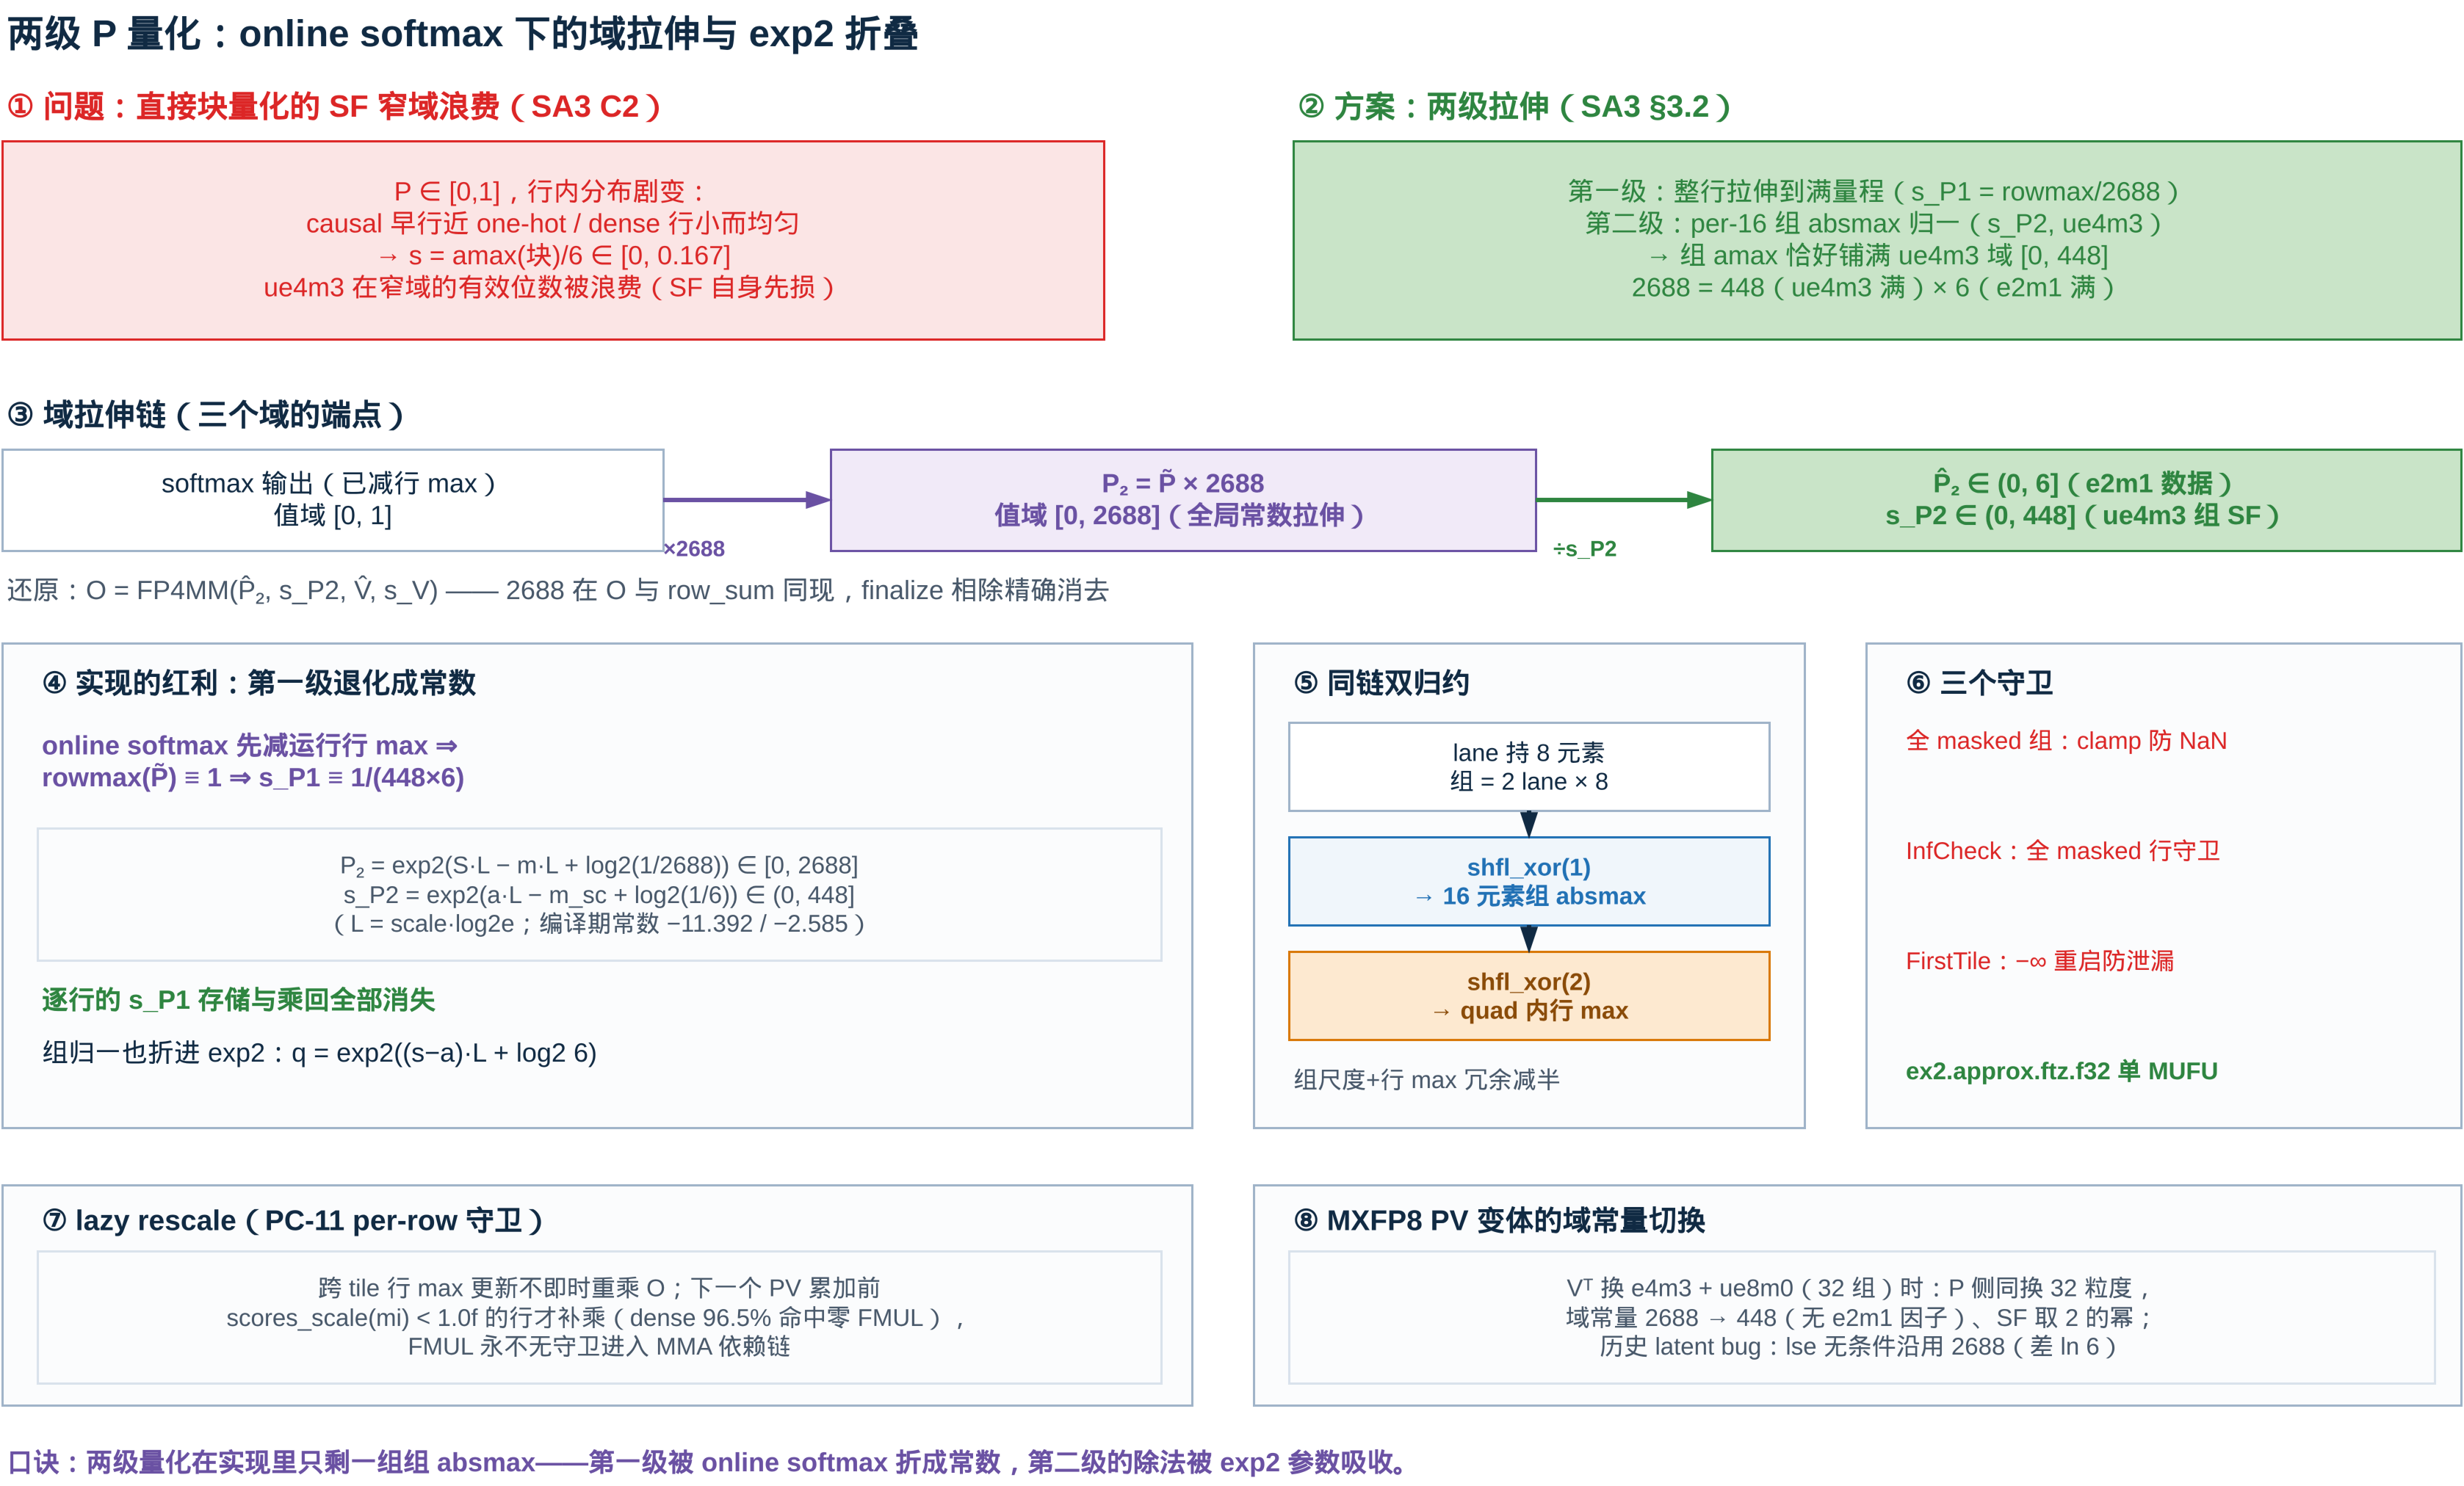
\includegraphics[width=0.98\textwidth]{figures/drawio/fig-32-1-two-level-p/fig-32-1-two-level-p.png}
  \begin{tikzpicture}
    \node[anchor=west, inner sep=0pt, align=left, font={\fontsize{7.4}{9.3}\selectfont \bfseries }] at (0.37,-0.354) {两级 P 量化：online softmax 下的域拉伸与 exp2 折叠};% w=17.094
    \node[anchor=west, inner sep=0pt, align=left, font={\fontsize{6.1}{7.7}\selectfont \bfseries \color{tkRed} }] at (0.37,-0.862) {(1) 问题：直接块量化的 SF 窄域浪费（SA3 C2）};% w=8.316
    \node[draw=tkRed, fill=tkFillRed, line width=0.5pt, minimum width=7.70cm, minimum height=1.39cm, inner sep=1pt, align=center, text width=7.64cm, font={\fontsize{5.2}{6.6}\selectfont \color{tkRed} }] at (4.22,-1.802) {P $\in$ [0,1]，行内分布剧变：\\causal 早行近 one-hot / dense 行小而均匀\\$\to$ s = amax(块)/6 $\in$ [0, 0.167]\\ue4m3 在窄域的有效位数被浪费（SF 自身先损）};
    \node[anchor=west, inner sep=0pt, align=left, font={\fontsize{6.1}{7.7}\selectfont \bfseries \color{tkGreen!70!black} }] at (9.394,-0.862) {(2) 方案：两级拉伸（SA3 \S{}3.2）};% w=8.162
    \node[draw=tkGreen, fill=tkFillGreen, line width=0.5pt, minimum width=8.16cm, minimum height=1.39cm, inner sep=1pt, align=center, text width=8.10cm, font={\fontsize{5.2}{6.6}\selectfont \color{tkGreen!70!black} }] at (13.475,-1.802) {第一级：整行拉伸到满量程（s\_P1 = rowmax/2688）\\第二级：per-group (16) absmax 归一（s\_P2, ue4m3）\\$\to$ 组 amax 恰好铺满 ue4m3 域 [0, 448]\\2688 = 448（ue4m3 满）$\times$ 6（e2m1 满）};
    \node[anchor=west, inner sep=0pt, align=left, font={\fontsize{6.1}{7.7}\selectfont \bfseries }] at (0.37,-3.018) {(3) 域拉伸链（三个域的端点）};% w=17.094
    \node[draw=gray!55, fill=none, line width=0.5pt, minimum width=4.62cm, minimum height=0.71cm, inner sep=1pt, align=center, text width=4.56cm, font={\fontsize{5.2}{6.6}\selectfont }] at (2.68,-3.619) {softmax 输出（已减行 max）\\值域 [0, 1]};
    \node[draw=tkPurple, fill=tkFillPurple, line width=0.5pt, minimum width=4.93cm, minimum height=0.71cm, inner sep=1pt, align=center, text width=4.87cm, font={\fontsize{5.2}{6.6}\selectfont \bfseries \color{tkPurple} }] at (8.624,-3.619) {P$_2$ = $\tilde{P}$ $\times$ 2688\\值域 [0, 2688]（全局常数拉伸）};
    \node[draw=tkGreen, fill=tkFillGreen, line width=0.5pt, minimum width=5.24cm, minimum height=0.71cm, inner sep=1pt, align=center, text width=5.17cm, font={\fontsize{5.2}{6.6}\selectfont \bfseries \color{tkGreen!70!black} }] at (14.938,-3.619) {$\hat{P}$$_2$ $\in$ (0, 6]（e2m1 数据）\\s\_P2 $\in$ (0, 448]（ue4m3 组 SF）};
    \node[anchor=west, inner sep=0pt, align=left, font={\fontsize{4.4}{5.5}\selectfont \bfseries \color{tkPurple} }] at (4.959,-3.958) {$\times$2688};% w=1.170
    \node[anchor=west, inner sep=0pt, align=left, font={\fontsize{4.4}{5.5}\selectfont \bfseries \color{tkGreen!70!black} }] at (11.18,-3.958) {$\div$s\_P2};% w=1.109
    \node[anchor=west, inner sep=0pt, align=left, font={\fontsize{5.2}{6.6}\selectfont \color{black!65} }] at (0.37,-4.25) {还原：O = FP4MM($\hat{P}$$_2$, s\_P2, $\hat{V}$, s\_V) ------ 2688 在 O 与 row\_sum 同现，finalize 相除精确消去};% w=17.094
    \node[draw=gray!55, fill=black!2, line width=0.5pt, minimum width=8.32cm, minimum height=3.39cm, inner sep=1pt, align=center, text width=8.25cm, font={\fontsize{5.7}{7.1}\selectfont }] at (4.528,-6.314) {};
    \node[anchor=west, inner sep=0pt, align=left, font={\fontsize{5.7}{7.1}\selectfont \bfseries }] at (0.616,-4.897) {(4) 实现的收益：第一级退化成常数};% w=7.854
    \node[anchor=west, inner sep=0pt, align=left, font={\fontsize{5.2}{6.6}\selectfont \bfseries \color{tkPurple} }] at (0.616,-5.452) {online softmax 先减运行行 max $\Rightarrow$\\rowmax($\tilde{P}$) $\equiv$ 1 $\Rightarrow$ s\_P1 $\equiv$ 1/(448$\times$6)};% w=7.854
    \node[draw=black!30, fill=black!2, line width=0.5pt, minimum width=7.85cm, minimum height=0.92cm, inner sep=1pt, align=center, text width=7.79cm, font={\fontsize{4.8}{6.0}\selectfont \color{black!65} }] at (4.543,-6.376) {P$_2$ = exp2(S$\cdot$L $-$ m$\cdot$L + log2(1/2688)) $\in$ [0, 2688]\\s\_P2 = exp2(a$\cdot$L $-$ m\_sc + log2(1/6)) $\in$ (0, 448]\\（L = scale$\cdot$log2e；编译期常数 $-$11.392 / $-$2.585）};
    \node[anchor=west, inner sep=0pt, align=left, font={\fontsize{5.2}{6.6}\selectfont \bfseries \color{tkGreen!70!black} }] at (0.616,-7.115) {逐行的 s\_P1 存储与乘回全部消失};% w=7.854
    \node[anchor=west, inner sep=0pt, align=left, font={\fontsize{5.2}{6.6}\selectfont }] at (0.616,-7.484) {组归一也折进 exp2：q = exp2((s$-$a)$\cdot$L + log2 6)};% w=7.854
    \node[draw=gray!55, fill=black!2, line width=0.5pt, minimum width=3.85cm, minimum height=3.39cm, inner sep=1pt, align=center, text width=3.79cm, font={\fontsize{5.7}{7.1}\selectfont }] at (11.042,-6.314) {};
    \node[anchor=west, inner sep=0pt, align=left, font={\fontsize{5.7}{7.1}\selectfont \bfseries }] at (9.363,-4.897) {(5) 同链双归约};% w=3.388
    \node[draw=gray!55, fill=none, line width=0.5pt, minimum width=3.36cm, minimum height=0.62cm, inner sep=1pt, align=center, text width=3.30cm, font={\fontsize{4.8}{6.0}\selectfont }] at (11.042,-5.482) {lane 持 8 元素\\组 = 2 lane $\times$ 8};
    \node[draw=tkBlue, fill=tkFillBlue, line width=0.5pt, minimum width=3.36cm, minimum height=0.62cm, inner sep=1pt, align=center, text width=3.30cm, font={\fontsize{4.8}{6.0}\selectfont \bfseries \color{tkBlue} }] at (11.042,-6.283) {shfl\_xor(1)\\$\to$ 16 元素组 absmax};
    \node[draw=tkOrange, fill=tkFillOrange, line width=0.5pt, minimum width=3.36cm, minimum height=0.62cm, inner sep=1pt, align=center, text width=3.30cm, font={\fontsize{4.8}{6.0}\selectfont \bfseries \color{tkOrange!75!black} }] at (11.042,-7.084) {shfl\_xor(2)\\$\to$ quad 内行 max};
    \node[anchor=west, inner sep=0pt, align=left, font={\fontsize{4.8}{6.0}\selectfont \color{black!65} }] at (9.363,-7.669) {组尺度+行 max 冗余减半};% w=3.388
    \node[draw=gray!55, fill=black!2, line width=0.5pt, minimum width=4.16cm, minimum height=3.39cm, inner sep=1pt, align=center, text width=4.10cm, font={\fontsize{5.7}{7.1}\selectfont }] at (15.477,-6.314) {};
    \node[anchor=west, inner sep=0pt, align=left, font={\fontsize{5.7}{7.1}\selectfont \bfseries }] at (13.644,-4.897) {(6) 三个守卫};% w=3.696
    \node[anchor=west, inner sep=0pt, align=left, font={\fontsize{4.8}{6.0}\selectfont \color{tkRed} }] at (13.644,-5.298) {全 masked 组：clamp 防 NaN};% w=3.696
    \node[anchor=west, inner sep=0pt, align=left, font={\fontsize{4.8}{6.0}\selectfont \color{tkRed} }] at (13.644,-6.068) {InfCheck：全 masked 行守卫};% w=3.696
    \node[anchor=west, inner sep=0pt, align=left, font={\fontsize{4.8}{6.0}\selectfont \color{tkRed} }] at (13.644,-6.838) {FirstTile：$-$$\infty$ 重启防泄漏};% w=3.696
    \node[anchor=west, inner sep=0pt, align=left, font={\fontsize{4.8}{6.0}\selectfont \bfseries \color{tkGreen!70!black} }] at (13.644,-7.608) {ex2.approx.ftz.f32 单 MUFU};% w=3.696
    \node[draw=gray!55, fill=black!2, line width=0.5pt, minimum width=8.32cm, minimum height=1.54cm, inner sep=1pt, align=center, text width=8.25cm, font={\fontsize{5.7}{7.1}\selectfont }] at (4.528,-9.178) {};
    \node[anchor=west, inner sep=0pt, align=left, font={\fontsize{5.7}{7.1}\selectfont \bfseries }] at (0.616,-8.655) {(7) lazy rescale（PC-11 per-row 守卫）};% w=7.854
    \node[draw=black!30, fill=black!2, line width=0.5pt, minimum width=7.85cm, minimum height=0.92cm, inner sep=1pt, align=center, text width=7.79cm, font={\fontsize{4.8}{6.0}\selectfont \color{black!65} }] at (4.543,-9.332) {跨 tile 行 max 更新不即时重乘 O；下一个 PV 累加前\\scores\_scale(mi) $<$ 1.0f 的行才补乘（dense 96.5\% 命中零 FMUL），\\FMUL 永不无守卫进入 MMA 依赖链};
    \node[draw=gray!55, fill=black!2, line width=0.5pt, minimum width=8.44cm, minimum height=1.54cm, inner sep=1pt, align=center, text width=8.38cm, font={\fontsize{5.7}{7.1}\selectfont }] at (13.336,-9.178) {};
    \node[anchor=west, inner sep=0pt, align=left, font={\fontsize{5.7}{7.1}\selectfont \bfseries }] at (9.363,-8.655) {(8) MXFP8 PV 变体的域常量切换};% w=8.008
    \node[draw=black!30, fill=black!2, line width=0.5pt, minimum width=8.01cm, minimum height=0.92cm, inner sep=1pt, align=center, text width=7.95cm, font={\fontsize{4.8}{6.0}\selectfont \color{black!65} }] at (13.367,-9.332) {V$^{\top}$ 换 e4m3 + ue8m0（32 组）时：P 侧同换 32 粒度，\\域常量 2688 $\to$ 448（无 e2m1 因子）、SF 取 2 的幂；\\历史 latent bug：lse 无条件沿用 2688（差 ln 6）};
    \node[anchor=west, inner sep=0pt, align=left, font={\fontsize{5.2}{6.6}\selectfont \bfseries \color{tkPurple} }] at (0.37,-10.349) {口诀：两级量化在实现里只剩一组组 absmax------第一级被 online softmax 折成常数，第二级的除法被 exp2 参数吸收。};% w=17.094
    \draw[tkPurple, line width=0.8pt, -{Stealth[length=2.2pt,width=1.8pt]}] (4.99,-3.619) -- (6.16,-3.619);
    \draw[tkGreen, line width=0.8pt, -{Stealth[length=2.2pt,width=1.8pt]}] (11.088,-3.619) -- (12.32,-3.619);
    \draw[black!75, line width=0.8pt, -{Stealth[length=2.2pt,width=1.8pt]}] (11.042,-5.79) -- (11.042,-5.975);
    \draw[black!75, line width=0.8pt, -{Stealth[length=2.2pt,width=1.8pt]}] (11.042,-6.591) -- (11.042,-6.776);
  \end{tikzpicture}
  \caption{两级 P 量化的域拉伸：online softmax 使第一级退化为全局常数
  $1/2688$ 并折进 exp2 shift；第二级 per-group (16) absmax 铺满 ue4m3 域，
  组归一化同样折进 exp2 参数。}
  \label{fig:32-1}
\end{figure}

\begin{figure}[htbp]
  \centering
  % was: 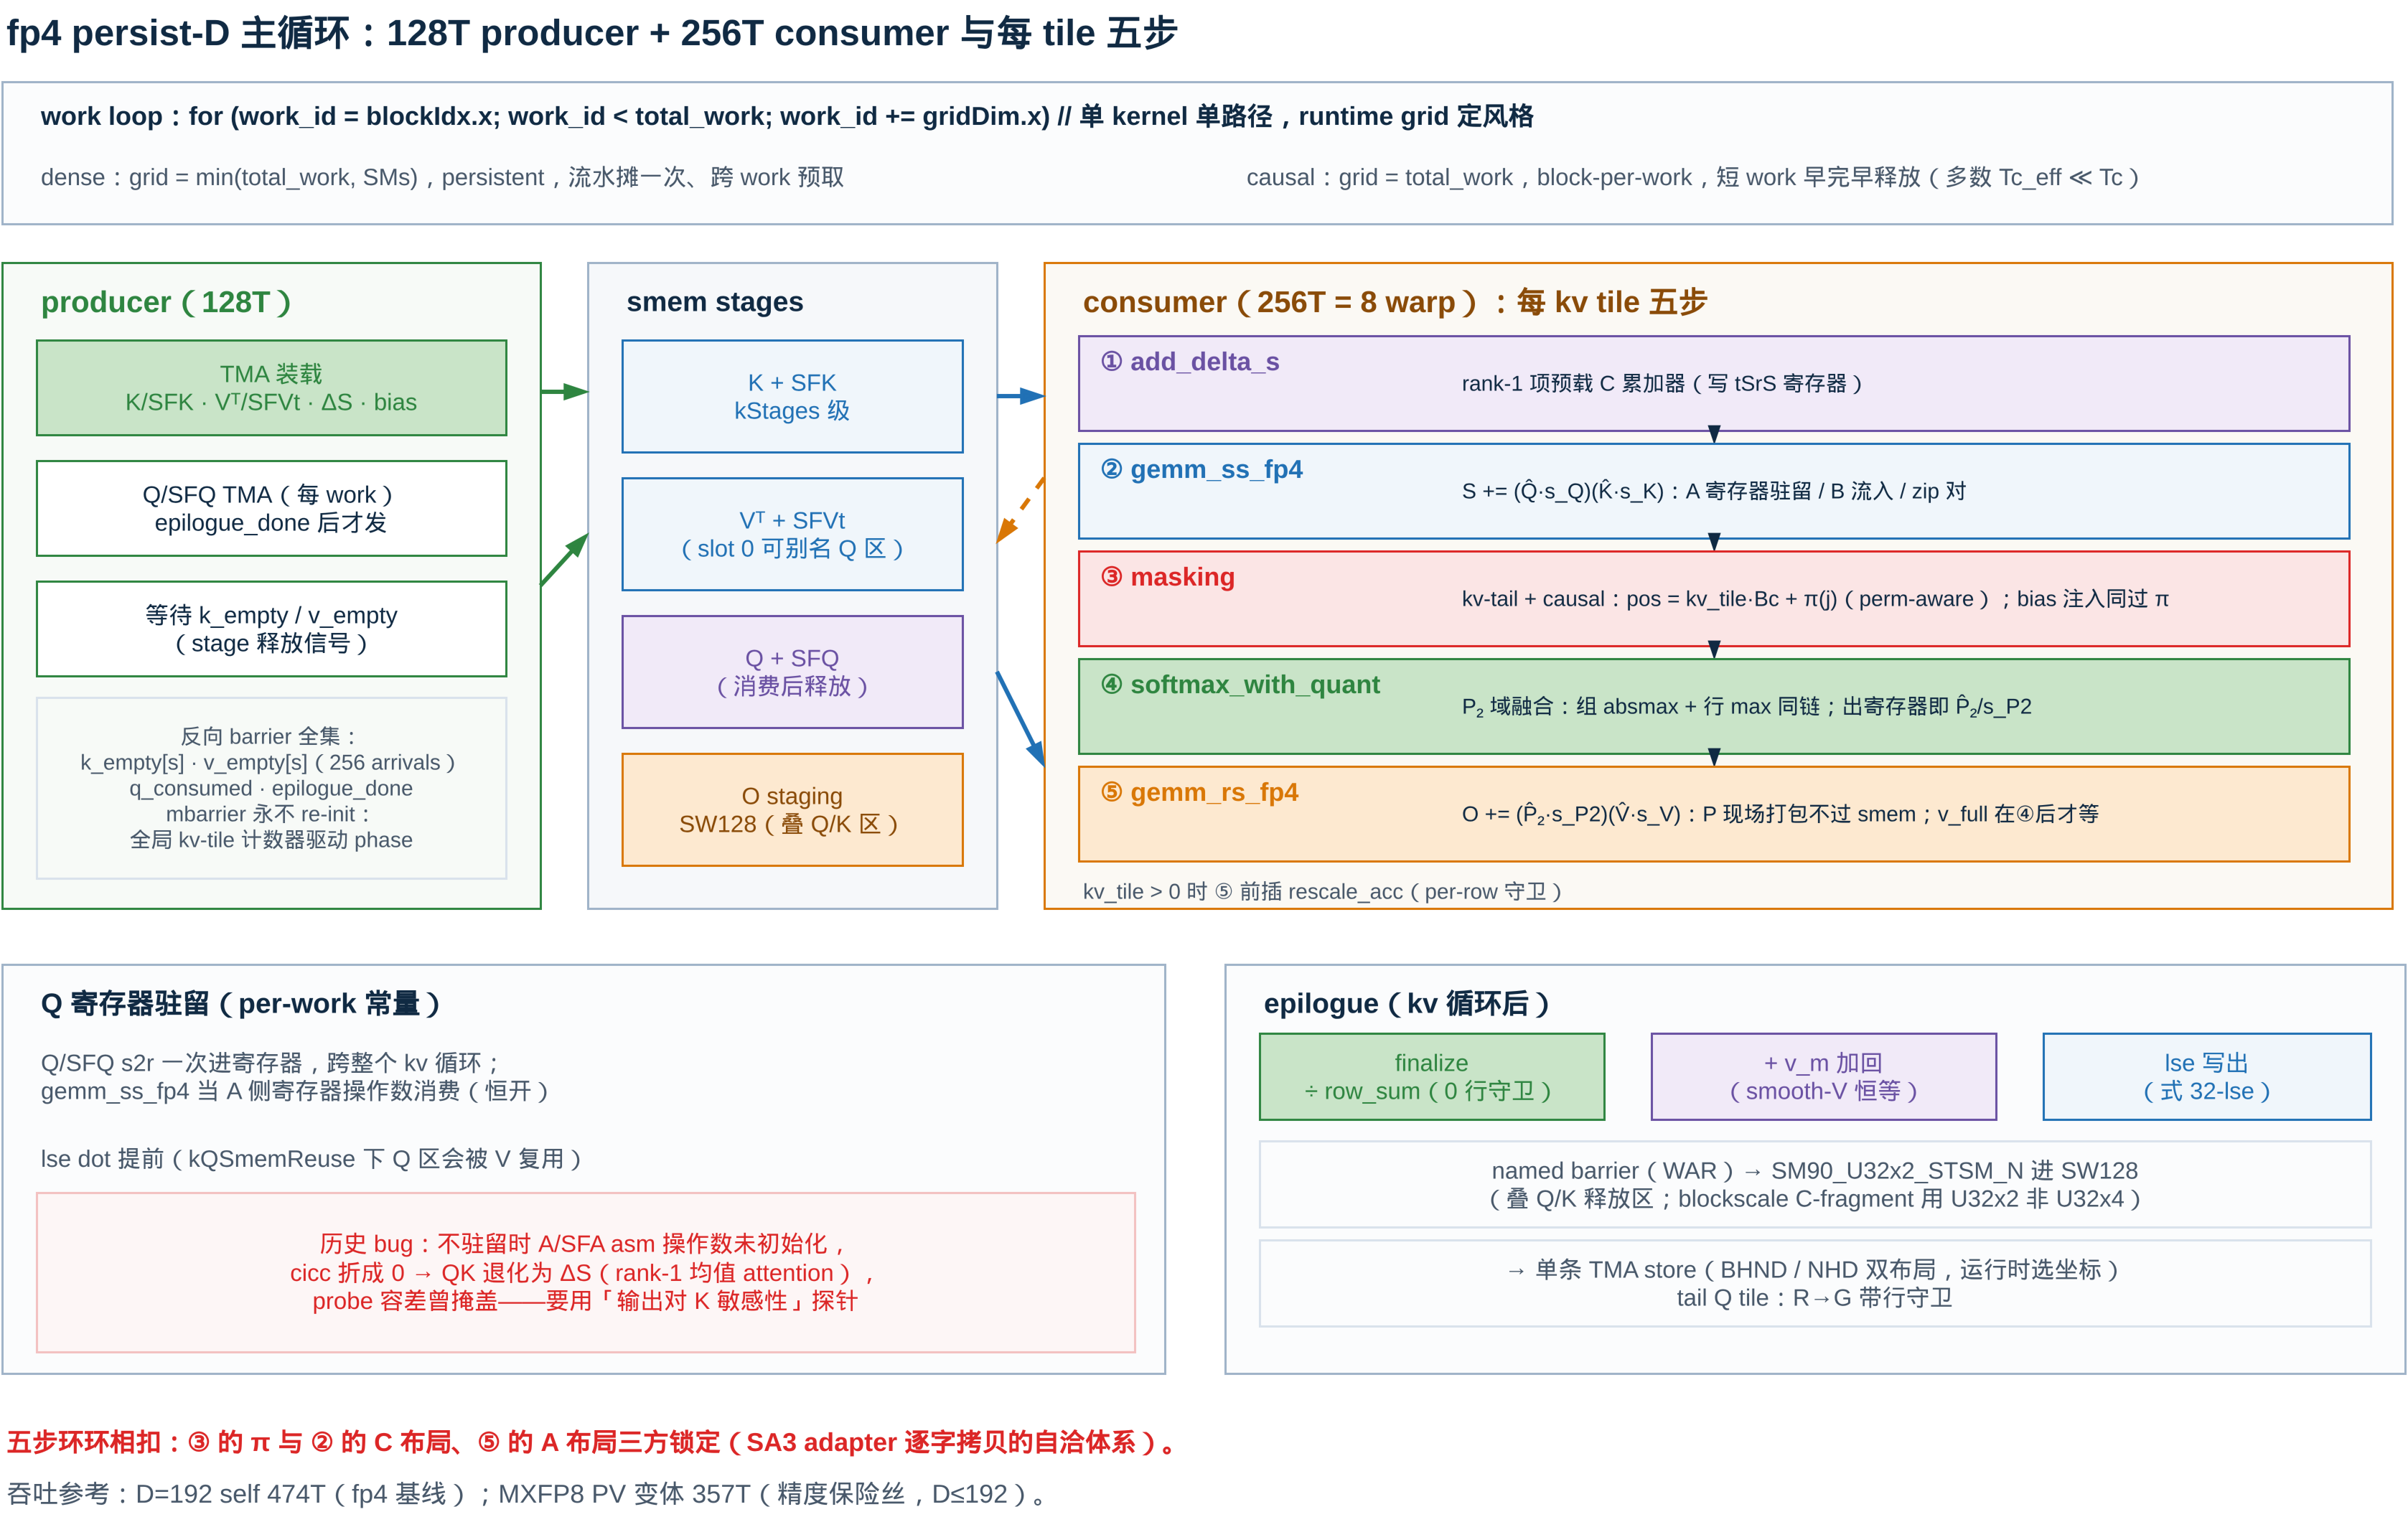
\includegraphics[width=0.98\textwidth]{figures/drawio/fig-32-2-persist-d-loop/fig-32-2-persist-d-loop.png}
  \begin{tikzpicture}
    \node[anchor=west, inner sep=0pt, align=left, font={\fontsize{7.4}{9.3}\selectfont \bfseries }] at (0.37,-0.354) {fp4 persist-D 主循环：128T producer + 256T consumer 与每 tile 五步};% w=17.094
    \node[draw=gray!55, fill=black!2, line width=0.5pt, minimum width=17.09cm, minimum height=1.02cm, inner sep=1pt, align=center, text width=17.03cm, font={\fontsize{5.7}{7.1}\selectfont }] at (8.917,-1.217) {};
    \node[anchor=west, inner sep=0pt, align=left, font={\fontsize{5.2}{6.6}\selectfont \bfseries }] at (0.616,-0.955) {work loop：for (work\_id = blockIdx.x; work\_id $<$ total\_work; work\_id += gridDim.x)   // 单 kernel 单路径，runtime grid 定风格};% w=16.478
    \node[anchor=west, inner sep=0pt, align=left, font={\fontsize{4.8}{6.0}\selectfont \color{black!65} }] at (0.616,-1.386) {dense：grid = min(total\_work, SMs)，persistent，流水摊一次、跨 work 预取};% w=8.008
    \node[anchor=west, inner sep=0pt, align=left, font={\fontsize{4.8}{6.0}\selectfont \color{black!65} }] at (9.24,-1.386) {causal：grid = total\_work，block-per-work，短 work 早完早释放（多数 Tc\_eff $\ll$ Tc）};% w=8.008
    \node[draw=tkGreen, fill=tkFillGreen!60!white, line width=0.5pt, minimum width=3.85cm, minimum height=4.62cm, inner sep=1pt, align=center, text width=3.79cm, font={\fontsize{5.7}{7.1}\selectfont }] at (2.295,-4.312) {};
    \node[anchor=west, inner sep=0pt, align=left, font={\fontsize{6.1}{7.7}\selectfont \bfseries \color{tkGreen!70!black} }] at (0.616,-2.279) {producer（128T）};% w=3.388
    \node[draw=tkGreen, fill=tkFillGreen, line width=0.5pt, minimum width=3.36cm, minimum height=0.68cm, inner sep=1pt, align=center, text width=3.30cm, font={\fontsize{4.8}{6.0}\selectfont \color{tkGreen!70!black} }] at (2.295,-2.895) {TMA 装载\\K/SFK $\cdot$ V$^{\top}$/SFVt $\cdot$ $\Delta$S $\cdot$ bias};
    \node[draw=tkGreen, fill=none, line width=0.5pt, minimum width=3.36cm, minimum height=0.68cm, inner sep=1pt, align=center, text width=3.30cm, font={\fontsize{4.8}{6.0}\selectfont }] at (2.295,-3.758) {Q/SFQ TMA（每 work）\\epilogue\_done 后才发};
    \node[draw=tkGreen, fill=none, line width=0.5pt, minimum width=3.36cm, minimum height=0.68cm, inner sep=1pt, align=center, text width=3.30cm, font={\fontsize{4.8}{6.0}\selectfont }] at (2.295,-4.62) {等待 k\_empty / v\_empty\\（stage 释放信号）};
    \node[draw=black!30, fill=tkFillGreen!60!white, line width=0.5pt, minimum width=3.36cm, minimum height=1.29cm, inner sep=1pt, align=center, text width=3.30cm, font={\fontsize{3.9}{4.9}\selectfont \color{black!65} }] at (2.295,-5.76) {反向 barrier 全集：\\k\_empty[s] $\cdot$ v\_empty[s]（256 arrivals）\\q\_consumed $\cdot$ epilogue\_done\\mbarrier 永不 re-init：\\全局 kv-tile 计数器驱动 phase};
    \node[draw=gray!55, fill=black!3, line width=0.5pt, minimum width=2.93cm, minimum height=4.62cm, inner sep=1pt, align=center, text width=2.86cm, font={\fontsize{5.7}{7.1}\selectfont }] at (6.021,-4.312) {};
    \node[anchor=west, inner sep=0pt, align=left, font={\fontsize{5.7}{7.1}\selectfont \bfseries }] at (4.805,-2.279) {smem stages};% w=2.464
    \node[draw=tkBlue, fill=tkFillBlue, line width=0.5pt, minimum width=2.43cm, minimum height=0.80cm, inner sep=1pt, align=center, text width=2.37cm, font={\fontsize{4.8}{6.0}\selectfont \color{tkBlue} }] at (6.021,-2.957) {K + SFK\\kStages 级};
    \node[draw=tkBlue, fill=tkFillBlue, line width=0.5pt, minimum width=2.43cm, minimum height=0.80cm, inner sep=1pt, align=center, text width=2.37cm, font={\fontsize{4.8}{6.0}\selectfont \color{tkBlue} }] at (6.021,-3.942) {V$^{\top}$ + SFVt\\（slot 0 可别名 Q 区）};
    \node[draw=tkPurple, fill=tkFillPurple, line width=0.5pt, minimum width=2.43cm, minimum height=0.80cm, inner sep=1pt, align=center, text width=2.37cm, font={\fontsize{4.8}{6.0}\selectfont \color{tkPurple} }] at (6.021,-4.928) {Q + SFQ\\（消费后释放）};
    \node[draw=tkOrange, fill=tkFillOrange, line width=0.5pt, minimum width=2.43cm, minimum height=0.80cm, inner sep=1pt, align=center, text width=2.37cm, font={\fontsize{4.8}{6.0}\selectfont \color{tkOrange!75!black} }] at (6.021,-5.914) {O staging\\SW128（叠 Q/K 区）};
    \node[draw=tkOrange, fill=tkFillOrange!60!white, line width=0.5pt, minimum width=9.64cm, minimum height=4.62cm, inner sep=1pt, align=center, text width=9.58cm, font={\fontsize{5.7}{7.1}\selectfont }] at (12.643,-4.312) {};
    \node[anchor=west, inner sep=0pt, align=left, font={\fontsize{6.1}{7.7}\selectfont \bfseries \color{tkOrange!75!black} }] at (8.07,-2.279) {consumer（256T = 8 warp）：每 kv tile 五步};% w=9.086
    \node[draw=tkPurple, fill=tkFillPurple, line width=0.5pt, minimum width=9.09cm, minimum height=0.68cm, inner sep=1pt, align=center, text width=9.02cm, font={\fontsize{5.7}{7.1}\selectfont }] at (12.613,-2.864) {};
    \node[anchor=west, inner sep=0pt, align=left, font={\fontsize{5.2}{6.6}\selectfont \bfseries \color{tkPurple} }] at (8.193,-2.71) {(1) add\_delta\_s};% w=2.618
    \node[anchor=west, inner sep=0pt, align=left, font={\fontsize{4.4}{5.5}\selectfont }] at (10.78,-2.864) {rank-1 项预载 C 累加器（写 tSrS 寄存器）};% w=6.314
    \node[draw=tkBlue, fill=tkFillBlue, line width=0.5pt, minimum width=9.09cm, minimum height=0.68cm, inner sep=1pt, align=center, text width=9.02cm, font={\fontsize{5.7}{7.1}\selectfont }] at (12.613,-3.634) {};
    \node[anchor=west, inner sep=0pt, align=left, font={\fontsize{5.2}{6.6}\selectfont \bfseries \color{tkBlue} }] at (8.193,-3.48) {(2) gemm\_ss\_fp4};% w=2.618
    \node[anchor=west, inner sep=0pt, align=left, font={\fontsize{4.4}{5.5}\selectfont }] at (10.78,-3.634) {S += ($\hat{Q}$$\cdot$s\_Q)($\hat{K}$$\cdot$s\_K)：A 寄存器驻留 / B 流入 / zip 对};% w=6.314
    \node[draw=tkRed, fill=tkFillRed, line width=0.5pt, minimum width=9.09cm, minimum height=0.68cm, inner sep=1pt, align=center, text width=9.02cm, font={\fontsize{5.7}{7.1}\selectfont }] at (12.613,-4.404) {};
    \node[anchor=west, inner sep=0pt, align=left, font={\fontsize{5.2}{6.6}\selectfont \bfseries \color{tkRed} }] at (8.193,-4.25) {(3) masking};% w=2.618
    \node[anchor=west, inner sep=0pt, align=left, font={\fontsize{4.1}{5.1}\selectfont }] at (10.78,-4.404) {kv-tail + causal：pos = kv\_tile$\cdot$Bc + $\pi$(j)（perm-aware）；bias 注入同过 $\pi$};% w=6.314
    \node[draw=tkGreen, fill=tkFillGreen, line width=0.5pt, minimum width=9.09cm, minimum height=0.68cm, inner sep=1pt, align=center, text width=9.02cm, font={\fontsize{5.7}{7.1}\selectfont }] at (12.613,-5.174) {};
    \node[anchor=west, inner sep=0pt, align=left, font={\fontsize{4.4}{5.5}\selectfont \bfseries \color{tkGreen!70!black} }] at (8.193,-5.02) {(4) softmax\_with\_quant};% w=2.618
    \node[anchor=west, inner sep=0pt, align=left, font={\fontsize{4.4}{5.5}\selectfont }] at (10.78,-5.174) {P$_2$ 域融合：组 absmax + 行 max 同链；出寄存器即 $\hat{P}$$_2$/s\_P2};% w=6.314
    \node[draw=tkOrange, fill=tkFillOrange, line width=0.5pt, minimum width=9.09cm, minimum height=0.68cm, inner sep=1pt, align=center, text width=9.02cm, font={\fontsize{5.7}{7.1}\selectfont }] at (12.613,-5.944) {};
    \node[anchor=west, inner sep=0pt, align=left, font={\fontsize{5.2}{6.6}\selectfont \bfseries \color{tkOrange} }] at (8.193,-5.79) {(5) gemm\_rs\_fp4};% w=2.618
    \node[anchor=west, inner sep=0pt, align=left, font={\fontsize{4.4}{5.5}\selectfont }] at (10.78,-5.944) {O += ($\hat{P}$$_2$$\cdot$s\_P2)($\hat{V}$$\cdot$s\_V)：P 现场打包不过 smem；v\_full 在(4)后才等};% w=6.314
    \node[anchor=west, inner sep=0pt, align=left, font={\fontsize{4.4}{5.5}\selectfont \color{black!65} }] at (8.07,-6.499) {kv\_tile $>$ 0 时 (5) 前插 rescale\_acc（per-row 守卫）};% w=9.086
    \node[draw=gray!55, fill=black!2, line width=0.5pt, minimum width=8.32cm, minimum height=2.93cm, inner sep=1pt, align=center, text width=8.25cm, font={\fontsize{5.7}{7.1}\selectfont }] at (4.528,-8.485) {};
    \node[anchor=west, inner sep=0pt, align=left, font={\fontsize{5.7}{7.1}\selectfont \bfseries }] at (0.616,-7.3) {Q 寄存器驻留（per-work 常量）};% w=7.854
    \node[anchor=west, inner sep=0pt, align=left, font={\fontsize{4.8}{6.0}\selectfont \color{black!65} }] at (0.616,-7.823) {Q/SFQ s2r 一次进寄存器，跨整个 kv 循环；\\gemm\_ss\_fp4 当 A 侧寄存器操作数消费（恒开）};% w=7.854
    \node[anchor=west, inner sep=0pt, align=left, font={\fontsize{4.8}{6.0}\selectfont \color{black!65} }] at (0.616,-8.408) {lse dot 提前（kQSmemReuse 下 Q 区会被 V 复用）};% w=7.854
    \node[draw=tkRed!45, fill=tkFillRed!60!white, line width=0.5pt, minimum width=7.85cm, minimum height=1.14cm, inner sep=1pt, align=center, text width=7.79cm, font={\fontsize{4.8}{6.0}\selectfont \color{tkRed} }] at (4.543,-9.225) {历史 bug：不驻留时 A/SFA asm 操作数未初始化，\\cicc 折成 0 $\to$ QK 退化为 $\Delta$S（rank-1 均值 attention），\\probe 容差曾掩盖------要用\textbf{输出对 K 敏感性}探针};
    \node[draw=gray!55, fill=black!2, line width=0.5pt, minimum width=8.44cm, minimum height=2.93cm, inner sep=1pt, align=center, text width=8.38cm, font={\fontsize{5.7}{7.1}\selectfont }] at (13.336,-8.485) {};
    \node[anchor=west, inner sep=0pt, align=left, font={\fontsize{5.7}{7.1}\selectfont \bfseries }] at (9.363,-7.3) {epilogue（kv 循环后）};% w=8.008
    \node[draw=tkGreen, fill=tkFillGreen, line width=0.5pt, minimum width=2.46cm, minimum height=0.62cm, inner sep=1pt, align=center, text width=2.40cm, font={\fontsize{4.8}{6.0}\selectfont \color{tkGreen!70!black} }] at (10.595,-7.823) {finalize\\$\div$ row\_sum（0 行守卫）};
    \node[draw=tkPurple, fill=tkFillPurple, line width=0.5pt, minimum width=2.46cm, minimum height=0.62cm, inner sep=1pt, align=center, text width=2.40cm, font={\fontsize{4.8}{6.0}\selectfont \color{tkPurple} }] at (13.398,-7.823) {+ v\_m 加回\\（smooth-V 恒等）};
    \node[draw=tkBlue, fill=tkFillBlue, line width=0.5pt, minimum width=2.34cm, minimum height=0.62cm, inner sep=1pt, align=center, text width=2.28cm, font={\fontsize{4.8}{6.0}\selectfont \color{tkBlue} }] at (16.139,-7.823) {lse 写出\\（式~\eqref{eq:32-lse}）};
    \node[draw=black!30, fill=black!2, line width=0.5pt, minimum width=7.95cm, minimum height=0.62cm, inner sep=1pt, align=center, text width=7.88cm, font={\fontsize{4.8}{6.0}\selectfont \color{black!65} }] at (13.336,-8.593) {named barrier（WAR）$\to$ SM90\_U32x2\_STSM\_N 进 SW128\\（叠 Q/K 释放区；blockscale C-fragment 用 U32x2 非 U32x4）};
    \node[draw=black!30, fill=black!2, line width=0.5pt, minimum width=7.95cm, minimum height=0.62cm, inner sep=1pt, align=center, text width=7.88cm, font={\fontsize{4.8}{6.0}\selectfont \color{black!65} }] at (13.336,-9.302) {$\to$ 单条 TMA store（BHND / NHD 双布局，运行时选坐标）\\tail Q tile：R$\to$G 带行守卫};
    \node[anchor=west, inner sep=0pt, align=left, font={\fontsize{5.2}{6.6}\selectfont \bfseries \color{tkRed} }] at (0.37,-10.441) {五步环环相扣：(3) 的 $\pi$ 与 (2) 的 C 布局、(5) 的 A 布局三方锁定（SA3 adapter 逐字拷贝的自洽体系）。};% w=17.094
    \node[anchor=west, inner sep=0pt, align=left, font={\fontsize{5.2}{6.6}\selectfont \color{black!65} }] at (0.37,-10.811) {吞吐参考：D=192 self 474T（fp4 基线）；MXFP8 PV 变体 357T（精度兜底，D$\leq$192）。};% w=17.094
    \draw[tkGreen, line width=0.8pt, -{Stealth[length=2.2pt,width=1.8pt]}] (4.22,-2.926) -- (4.558,-2.926);
    \draw[tkGreen, line width=0.8pt, -{Stealth[length=2.2pt,width=1.8pt]}] (4.22,-4.312) -- (4.558,-3.942);
    \draw[black!75, line width=0.5pt, -{Stealth[length=2.2pt,width=1.8pt]}] (12.613,-3.203) -- (12.613,-3.296);
    \draw[black!75, line width=0.5pt, -{Stealth[length=2.2pt,width=1.8pt]}] (12.613,-3.973) -- (12.613,-4.066);
    \draw[black!75, line width=0.5pt, -{Stealth[length=2.2pt,width=1.8pt]}] (12.613,-4.743) -- (12.613,-4.836);
    \draw[black!75, line width=0.5pt, -{Stealth[length=2.2pt,width=1.8pt]}] (12.613,-5.513) -- (12.613,-5.606);
    \draw[tkBlue, line width=0.8pt, -{Stealth[length=2.2pt,width=1.8pt]}] (7.484,-2.957) -- (7.823,-2.957);
    \draw[tkBlue, line width=0.8pt, -{Stealth[length=2.2pt,width=1.8pt]}] (7.484,-4.928) -- (7.823,-5.606);
    \draw[tkOrange, line width=0.8pt, dashed, -{Stealth[length=2.2pt,width=1.8pt]}] (7.823,-3.542) -- (7.484,-4.004);
  \end{tikzpicture}
  \caption{fp4 persist-D 主循环数据流（128T producer + 256T consumer）：
  每 kv tile 的五步（$\Delta S$ 预载 $\to$ QK $\to$ masking $\to$ 融合
  softmax/P 量化 $\to$ PV），barrier 永不 re-init，grid 由 runtime 定
  persistent 或 block-per-work。}
  \label{fig:32-2}
\end{figure}

\FloatBarrier

\section{性能分析}

\subsection{本机 e2e（fp4 vs SDPA）}

表~\ref{tab:32-mxfp8} 汇总 \texttt{--fp4-pv-mm-type fp8} 变体（数据落
盘 \texttt{.tmp/book-bench/ch32/}）；fp4 基线表见
第~\ref{ch:31}~章表~\ref{tab:31-bench}（self 1.49--2.11x、causal 1.25--1.61x，
16 格全绿）。

\begin{table}[H]
  \centering
  \caption{MXFP8 PV 变体 vs fp4 基线（PRO 5000，$B{=}1,H{=}32,N{=}8192$，
  fp16 口径，allclose 全绿；末列加速比为对 SDPA 的 $T_{\mathrm{SDPA}}/T_{\mathrm{mxfp8}}$，
  SDPA 时间见第~\ref{ch:31}~章表~\ref{tab:31-bench}）}
  \label{tab:32-mxfp8}
  \begin{tabular}{@{}rlllll@{}}
    \toprule
    $D$ & mxfp8 self (ms) & vs fp4 & mxfp8 causal (ms) & vs fp4 & 加速比
    (self/causal) \\
    \midrule
    64  & 2.24 & $+39\%$ & 1.41 & $+31\%$ & 1.07x / 0.96x \\
    128 & 3.47 & $+38\%$ & 2.17 & $+30\%$ & 1.47x / 1.24x \\
    192 & 4.62 & $+33\%$ & 3.06 & $+28\%$ & 1.55x / 1.25x \\
    \bottomrule
  \end{tabular}
\end{table}

MXFP8 PV 付出 28--39\% 的代价：$V^\top$ 数据 8 bit 带宽翻倍、atom 换
\texttt{m16n8k128}，两者吞吐相近但带宽直接体现在 e2e。它的定位是
\textbf{精度兜底}（$D\le192$ 的 smem 预算内），不是性能选项
（第~\ref{ch:31}~章 31.6 同结论）。

\subsection{fp4 对 fp8 的相对收益}

历史对照（RFC/skill 记录口径，非本机当日）：attn kernel 本身 fp4 比
fp8 快 $\sim$23\%：blockscale mxf4nvf4 吞吐与 fp8 dense 相当，收益
全部来自带宽（K/V/SF 字节减半以上）；D=192 的 e2e 比值
self 1.47x / causal 1.29x / gqa 1.50x。本机同日对照可复算：fp4 D=192
self 3.48ms（表~\ref{tab:31-bench}）对 fp8 persist-D 同 shape 的第~\ref{ch:29}~章 29.6 节实测表
数据（4.58\,ms）作比，得 1.32$\times$（该 shape 在 861d75e 上有正确性 bug、
速度仅供参考，见 29.7.1）。

\subsection{已落地与已证伪的微优化}

已落地：条件 rescale（PC-11 per-row 守卫，dense 96.5\% 命中，
-4.9\%；attn-mask 场景再 -3.7/-4.7\%）、\texttt{ex2.approx.ftz.f32}
（消 ptxas range 胶水，-5.9\%）、regalloc 按 D 门控（$D\le128$ 用
\texttt{alloc<224>}，$D\ge192$ 必须 232）。

已证伪（默认关闭/代码保留，勿重复）：Q smem 复用（fp4 的 L1TEX
sector hit 已 96.75\% 饱和，fp8 的前提不成立，实测 +1.8\% 回退，
\texttt{attn\_traits.cuh} L19--28 注释，与 fp8 章的同名机制结论相
反）。rescale merge in-place（把 FMUL 拉进 MMA 依赖
链，+1.7\%）。V/SFV 首块 s2r 提前藏进 softmax（PC-4：+1.3--1.7\% 净
负，LDSM 目的寄存器跨 softmax 链拉长 live-range；NCU 证实 B 供给非
瓶颈，wait 主体在 A 操作数串行链，也是 persist-D 微优化到顶的标志）。

\section{实践经验}

SA3 的 fragment adapter 是一块经验锁定的整体。kv\_perm32、$\Delta S$
槽位算术、\texttt{LayoutP}/\texttt{LayoutSFP} 打包、$V^\top$ 转置存储：
这些项相互补偿、自洽成体系（头注释 L25--37：empirical
lock 在 \texttt{.tmp} 的对齐探针里逐项验证过，dense e2e 与 dequant 仿真
一致）。逐字拷贝 + 只修 masking 是正确的移植方式；单独\textbf{改进}其中
一项会破坏补偿关系。

e2m1 的相对量化误差（主区间 $\sim$20\%、
0.75 中点最坏 $\sim$33\%）使 P/V 两级误差叠
加后 causal 尖峰行 max\_abs 天然 0.5--0.75（probe 仿真与 kernel 同
级，格式固有）；SA3 论文自身用 cosine 评估。工程验收看 mean\_abs
（0.014--0.03）与容差（dense 0.15 / causal 0.70），用 fp8 的容差卡
fp4 会全部不通过。hybrid（fp16 前 $n_{early}$ 行）是尖峰行的工程解法
（b0/b1 误差 2.6/0.99 $\to$ 0.000/0.001，剩余长尾由 V 量化主导）。

\section{常见坑}

\begin{enumerate}[itemsep=2pt,topsep=2pt]
  \item \textbf{masking 不 perm-aware}：causal 谓词按原始列 index 判
        定，$N{=}512$ max\_abs 3.3（上游 SA3 真实 bug；本章 32.4.3 的
        $pos$ 公式）。
  \item \textbf{mxfp8 域常量}：PV 换 mxfp8 后 lse 仍用 2688——差
        $\ln6$ 的 latent bug，按 \texttt{kPvMxfp8} 编译期分流域常量。
  \item \textbf{mbarrier re-init 是 UB}：跨 work 循环里对活跃 barrier
        re-initialize 行为未定义（PTX ISA 9.7.13.15.9），用全局 tile
        计数器驱动 phase。
  \item \textbf{stale AbsMaxP}：组 absmax 寄存器跨 tile/跨 work 复用，
        每 FirstTile 必须从 $-\infty$ 重新起步（L151--154 注释），
        否则上个 work 的尺度泄漏进当前行。
  \item \textbf{未初始化 asm 操作数被折叠}：Q 不驻留寄存器时 cicc 把
        A/SFA 操作数折成 0，QK 静默退化（32.4.2 的历史 bug）。
  \item \textbf{subbyte smem 指针}：e2m1 tensor 必须
        \texttt{make\_smem\_ptr}，裸 \texttt{reinterpret\_cast} 地址差
        2 倍、stage$\ge$1 TMA 越界（第~\ref{ch:31}~章 31.4.6）。
\end{enumerate}

\section{面试要点速查}

\begin{enumerate}[itemsep=2pt,topsep=2pt]
  \item 两级 P 量化：$s_{P1}=\mathrm{rowmax}/2688$、
        $\tilde P_2\in[0,2688]$、$s_{P2}$ per-group (16) ue4m3；2688 =
        448（ue4m3 满）$\times$ 6（e2m1 满）。
  \item online softmax 的退化收益：行 max 恒 1 $\Rightarrow$ 第一级变
        全局常数折进 exp2 shift——两级量化在实现里只剩一组 absmax。
  \item 组归一化折进 exp2 参数：$q=\exp_2((s-a)L+\log_2 6)$，rcp 与
        FMUL 段消失；row\_sum 用 FMA 吸收 $s_{P2}$。
  \item 2688 的消去：$O$ 与 row\_sum 同带常数，finalize 相除精确抵消。
  \item dense persistent / causal block-per-work：单 kernel 单路径，
        runtime grid 定风格；barrier phase 由全局 tile 计数器驱动。
  \item blockscale QK/PV 的 A 侧差异：Q 寄存器驻留（per-work 常量）、
        P 寄存器现场打包（quantize\_and\_pack\_p），B 侧才走 smem
        stage。
  \item fp4 vs fp8 的收益来源：MMA 吞吐持平、带宽减半——memory-bound
        attention 的收益逻辑。
\end{enumerate}

\section{最小测试与动手实验}

\begin{lstlisting}[style=console]
export CUDA_VISIBLE_DEVICES=7 FFPA_CUDA_ALLOW_SMALL_D=1
python -m ffpa_attn.bench --fwd-backend cuda --cuda-impl fp4 \
  --tasks self-attn causal --D 192 --no-bwd --show-allclose
# MXFP8 PV（精度保险丝，D<=192）：
python -m ffpa_attn.bench --fwd-backend cuda --cuda-impl fp4 \
  --tasks self-attn causal --D 192 --no-bwd --show-allclose \
  --fp4-pv-mm-type fp8
\end{lstlisting}

\begin{enumerate}[itemsep=2pt,topsep=2pt]
  \item \textbf{两级域验证}：读 \texttt{fp4\_pscale.cuh} L117--128 的
        三个编译期常数，手推
        式~\ref{eq:32-p2-domain} 的两个值域端点（$P_2=2688$ 当
        $s=m$；$s_{P2}=448$ 当组 absmax $=$ 行 max）。
  \item \textbf{mxfp8 A/B}：复现表~\ref{tab:32-mxfp8} 的三档 D，验证
        $D{=}256$ 被 traits 的 smem 断言拒绝。
  \item \textbf{causal 风格对照}：读 \texttt{launch/cute\_fp4\_persist\_d.cuh} 的
        grid 选择（\texttt{causal ? total\_work : min(...)}），解释为
        什么 causal 的多数 work 选 block-per-work。
  \item \textbf{InfCheck 场景}：构造 $N_q>N_{kv}$ 的 cross 输入跑
        causal，确认左上角全 masked 行的 lse/O 有限（无 NaN）。
\end{enumerate}

\section*{延伸阅读}
\addcontentsline{toc}{section}{延伸阅读}

\begin{itemize}[itemsep=0pt,topsep=2pt]
  \item \texttt{cute/fp4/sm\_120/persist\_d.cuh} 头注释（L1--55）：
        数学链、列对齐锁定、两级 P、subbyte。
  \item \texttt{cute/fp4/fp4\_pscale.cuh} L117--195：融合 softmax 的
        域折叠与 shuffle 链。
  \item \texttt{cute/fp4/fp4\_gemm.cuh} L91--218：\texttt{gemm\_ss\_fp4}
        与 \texttt{gemm\_rs\_fp4} 的流水与 barrier 协议。
  \item SageAttention3 论文 §3.2（两级量化）与 Algorithm 1（完整数值
        链）；sm\_120 split-D 与 M4N2 家族见第~\ref{ch:30}~章的 fp8
        同构实现。
\end{itemize}

% ch33-fp8-fp4-bench.tex — FP8/FP4 性能实战：bench、精度与生态（RFC-K7）
% 源码：ffpa-attn(861d75e) bench/bench_fp8.py(719L) + bench/bench_fp4.py(652L) + ffpa_attn.bench CLI
\chapter{FP8/FP4 性能实战：Bench、精度与生态}\label{ch:33}

\section{本章导读}

第~\ref{ch:29}--\ref{ch:32}~章讲完了 fp8/fp4 attention 的全部实现；
本章讲怎么度量与选用它们。这是量化 attention 的最后一步：
一个不公平的 bench 能把 2x 加速测成 0.5x（功耗墙、参照漂移、preset
隐藏成本），一个错误的容差能把好 kernel 判成精度不合格（用 fp8 的
容差去卡 fp4）。本章沿三条线索展开：
\begin{enumerate}[itemsep=0pt,topsep=2pt]
  \item \textbf{口径}：speedup 怎么算才公平（参照后端、min-of-N、
        pre-heat、no\_grad）；精度怎么报才有信息量（布尔 allclose 之外
        的 rel\_err/max\_abs 体系）；
  \item \textbf{矩阵}：bench CLI 的全 knob 空间与实测——fp8/fp4 在
        self/causal/gqa/cross $\times$ D$\in[64,512]$ 上的完整矩阵，
        knob（QK int8/fp8、PV f16/f32、量化粒度、hybrid）的边际效应；
  \item \textbf{生态}：Cache-DiT $\times$ FFPA 的端到端集成——量化
        attention 在真实扩散模型管线里怎么落地。
\end{enumerate}
素材锚定 ffpa-attn \texttt{861d75e} 的 \texttt{bench/bench\_fp8.py}、
\texttt{bench/bench\_fp4.py} 与 \texttt{ffpa\_attn.bench} CLI；本机
实测平台 RTX PRO 5000（sm\_120），5090 数据引自仓库
\texttt{docs/assets/perf/} 归档实测图。

\section{问题与动机}

度量陷阱一：参照系。speedup 是比值，分子分母任何一个漂移，
结论就作废。三个具体来源：

\begin{itemize}[itemsep=0pt,topsep=2pt]
  \item \textbf{本 bench 的 \texttt{auto} 参照随 D 换挡}：脚本在
        $D\le256$ 时选择 FA2，更大 D 选择 MATH（materialize 整个
        $N_q\times N_{kv}$ 矩阵），参照时间膨胀数倍：D=512 的 3x
        加速里有一大半是 MATH 慢，不是量化快（\texttt{bench\_fp8.py}
        L153--160 的 \texttt{resolve\_sdpa\_backend}）。这是
        \texttt{--sdpa-backend auto} 的显式解析规则，不是 PyTorch
        SDPA 的通用回退规则。
  \item \textbf{GPU 状态污染}：5090 类高功耗卡上，前一个高功耗负载
        会把后一个测试压进降频区（实测 FFPA kernel 撞功耗墙
        2932$\to$2445MHz，-17\%）；A/B 两轮的 SDPA 参照必须吻合
        （$\pm1\%$），否则整轮作废。
  \item \textbf{preset 隐藏成本}：对比双方的功能集不对齐时，\textbf{慢}
        可能只是\textbf{多做了事}：hybrid（fp16 前缀行）与 smooth-V
        都是 FFPA 独有的精度功能，开着测速度对 Sage 不公平，对
        用户也是误导。
\end{itemize}

\begin{figure}[H]
\centering
\begin{tikzpicture}[font=\scriptsize]
  \definecolor{gearred}{RGB}{178,34,34}
  \fill[gray!14] (0,0) rectangle (3.857,4.8);
  \fill[gray!32] (3.857,0) rectangle (9.0,4.8);
  \node[align=center, font=\tiny] at (1.95,4.42) {SDPA-FA2\\（融合 kernel）};
  \node[align=center, font=\tiny] at (6.45,4.42) {SDPA-MATH：materialize\\$N_q{\times}N_{kv}$（8192$^2$）矩阵};
  \draw[dashed, thick] (3.857,0) -- (3.857,4.8);
  \node[above, font=\tiny] at (3.857,4.82) {换挡点 $D{=}256$};
  \draw[->] (0,0) -- (9.6,0);
  \node[below] at (9.3,-0.05) {$D$};
  \draw[->] (0,0) -- (0,5.3);
  \node[left] at (0.03,5.15) {speedup};
  \foreach \dx/\dl in {0/64,1.286/128,3.857/256,9.0/512}{
    \draw (\dx,0) -- (\dx,-0.07);
    \node[below, font=\tiny, inner sep=1pt] at (\dx,-0.08) {\dl};
  }
  \foreach \dy/\dl in {0/1.0,1.091/1.5,2.182/2.0,3.273/2.5,4.364/3.0}{
    \draw (0,\dy) -- (-0.07,\dy);
    \node[left, font=\tiny, inner sep=1pt] at (-0.08,\dy) {\dl};
  }
  \draw[gray, thin] (0,0.567) -- (1.286,1.527) -- (3.857,0.655) -- (9.0,4.327);
  \fill (0,0.567) circle (0.05);
  \fill (1.286,1.527) circle (0.05);
  \fill (3.857,0.655) circle (0.05);
  \fill (9.0,4.327) circle (0.05);
  \node[above right=-1pt and 1pt, font=\tiny] at (0,0.567) {1.26$\times$};
  \node[above right=-1pt and 1pt, font=\tiny] at (1.286,1.527) {1.70$\times$};
  \node[below right=-1pt and 1pt, font=\tiny] at (3.857,0.655) {1.30$\times$};
  \node[above left=-1pt and 1pt, font=\tiny] at (9.0,4.327) {2.98$\times$};
  \draw[->, gearred, thick] (4.1,0.95) to[bend left=18] (8.75,4.05);
  \node[gearred, align=center, font=\tiny] at (6.35,2.1)
    {同为 split-D 家族（D=256/512）\\1.30$\to$2.98 的跳变主要来自\\参照换挡（右图分解）};
  \node[anchor=south, font=\scriptsize\bfseries] at (4.8,5.45)
    {本 bench \texttt{auto} 的 SDPA 参照换挡带（表~\ref{tab:33-fp8-matrix} self 行）};
  \begin{scope}[xshift=10.5cm]
    \draw[->] (0,0) -- (4.4,0);
    \draw[->] (0,0) -- (0,7.4);
    \node[left, font=\tiny] at (-0.05,7.2) {ms};
    \fill[gray!22] (0.40,0) rectangle (1.40,2.28);
    \fill[gray!45] (1.90,0) rectangle (2.90,2.96);
    \fill[gray!68] (3.40,0) rectangle (4.40,6.80);
    \node[above, font=\tiny] at (0.9,2.32) {21.71};
    \node[above, font=\tiny] at (2.4,3.00) {$\approx$28.2};
    \node[above, font=\tiny] at (3.9,6.84) {64.74};
    \node[below, font=\tiny, align=center, inner sep=1pt] at (0.9,-0.08) {FFPA\\split-D};
    \node[below, font=\tiny, align=center, inner sep=1pt] at (2.4,-0.08) {SDPA 若 FA2 级\\（外推）};
    \node[below, font=\tiny, align=center, inner sep=1pt] at (3.9,-0.08) {SDPA-MATH\\实测};
    \node[anchor=west, align=left, text width=1.6cm, font=\tiny] at (4.5,4.6)
      {$64.74/21.71$\\{$=$} 2.98$\times$\\{$=$} 1.30$\times$（真）\\{$\times$} 2.29$\times$（参照）};
    \node[anchor=south, font=\scriptsize\bfseries] at (2.2,7.7) {D=512 self 的 2.98$\times$ 归因};
  \end{scope}
  \node[anchor=north west, align=left, text width=14.5cm, font=\tiny] at (0,-1.20)
    {本 bench \texttt{auto} 口径下，\textbf{3$\times$}里一大半是 MATH 参照自身的低效，
     不是量化快（坑 6）——报告 $D{>}256$ 的 speedup 必须注明该参照换挡。外推口径：
     D=256 同为 split-D 家族且参照是 FA2，实测 1.30$\times$ 用作\textbf{真加速}估计；
     $21.71\times1.30\approx28.2$ms，$64.74/28.2\approx2.29\times$。};
\end{tikzpicture}
\caption{参照系视角看表~\ref{tab:33-fp8-matrix} 的 self 行。左：本 bench 的
\texttt{--sdpa-backend auto} 在 $D\le256$ 时选择 FA2，更大 $D$ 选择 MATH
（materialize $N_q\times N_{kv}$ 矩阵）；四个 speedup 点
（1.26/1.70/1.30/2.98$\times$）落在换挡带上，D=512 的跳变包含参照换挡的贡献。
右：D=512 的 $2.98\times$ 归因——以 D=256 同家族（split-D、FA2 参照）实测
1.30$\times$ 为真加速估计，MATH 参照自身再慢 $\times$2.29：
\textbf{3$\times$}的大头是参照低效（坑 6）。}
\label{fig:33-sdpa-gear}
\end{figure}

度量陷阱二：精度口径。allclose 是布尔值，信息量极低：

\begin{itemize}[itemsep=0pt,topsep=2pt]
  \item fp4 的 e2m1 网格噪声决定了它的容差天然比 fp8 宽一个量级
        （dense 0.15 / causal 0.70 vs fp8 的 0.05），拿错档的容差
        会把合格的实现误判为不合格。
  \item 只看均值不看 max 会漏掉 causal 早期行这类结构性
        误差（第~\ref{ch:27}~章 27.3.7 节的 e2m1 网格噪声）。
  \item 推理 bench 必须 \texttt{no\_grad}：grad-on 会强制走完整
        autograd 链（每调用多 $\sim$30$\mu$s Python 开销，
        \texttt{bench\_ms} 注释口径），测出的
        是训练链路而非 kernel。
\end{itemize}

\noindent{\footnotesize 注：本节与坑 3 的功耗墙频率（2932$\to$2445MHz）
及顺序差（466--491$\mu$s）为本机补充实测（2026-08，单卡 PRO 5000），
原始 stdout 未随书归档。\par}

\section{数学原理}

\subsection{speedup 与有效 TFLOPS}

kernel 级 speedup 定义为同形状下参照与被测的耗时比。
\begin{equation}
  S=\frac{T_{\mathrm{SDPA}}}{T_{\mathrm{FFPA}}},\qquad
  T=\min_{i\in[1,N]}\;t_i\;\;(\text{min-of-}N,\ N\ge5)
\end{equation}
本章用 min-of-N 而非均值做 kernel 对比，取较少受时钟迁移、后台进程等
毛刺影响的一次计时，估计当前形状下的可达耗时下界。它不是通用推理延迟
合同，也不能替代 median、p95 等稳态或尾延迟指标。

有效算力用 attention 前向 FLOPS 归一。
\begin{equation}
  \mathrm{FLOPs}=4\,N_qN_{kv}DH_q\cdot\delta_{\mathrm{causal}},\qquad
  \delta_{\mathrm{causal}}=
  \begin{cases}1 & \text{dense}\\[2pt] \tfrac{1}{2}+\tfrac{1}{2N_{kv}} & \text{causal}\end{cases}
\end{equation}
（QK$^\top$ 与 PV 各占 $2N_qN_{kv}DH_q$；causal 按三角 mask 减半。
此因子在方阵 $N_q=N_{kv}$ 下与 \texttt{\_flops.py} 的精确 tail 对齐
计数一致。FFPA 的非方阵 causal 将 query 行对齐 KV 尾部（mask 右下角对齐）；
当 $N_q\le N_{kv}$ 时，第 $i$ 行（从 0 开始）有 $N_{kv}-N_q+i+1$ 个有效位置，
故精确因子为 $1-(N_q-1)/(2N_{kv})$。本章 bench 的 causal 均为方阵。）
注意这是\textbf{数学} FLOPS：量化 kernel 实际吞吐的是低位宽 MMA，
$S>1$ 的来源是同样的数学量改由快得多的数据通路完成。

\subsection{端到端摊销}

单算子加速换算成管线加速要看占比。设管线总时 $T$，attention 占
$\alpha$，则端到端 speedup 上界为：
\begin{equation}
  S_{\mathrm{e2e}}=\frac{T}{T-\alpha T(1-1/S_{\mathrm{attn}})}
  \xrightarrow{\ \alpha\to1\ }S_{\mathrm{attn}}
  \label{eq:33-e2e}
\end{equation}
$\alpha=0.3$、$S_{\mathrm{attn}}=2.5$x 时 $S_{\mathrm{e2e}}\approx1.22$x：
attention 只省下 $0.3T\times0.6=0.18T$，总时从 $T$ 降到
$0.82T$。这解释了为什么扩散模型（attention 占比高、D 偏小）是量化 attention
的第一应用场景，也是 Cache-DiT 集成（33.7 节）的价值前提。

\begin{figure}[H]
\centering
\begin{tikzpicture}[font=\scriptsize]
  \def\axw{8.0}
  \def\aysc{2.909}
  \draw[->] (0,0) -- ({\axw+0.30},0);
  \draw[->] (0,0) -- (0,7.05);
  \node[left, font=\tiny, align=right] at (-0.05,6.95) {$S_{\mathrm{e2e}}$};
  \foreach \sv in {1.0,1.5,2.0,2.5,3.0}{
    \pgfmathsetmacro{\yv}{(\sv-1)*\aysc}
    \draw (-0.07,\yv) -- (0.07,\yv);
    \node[left, font=\tiny, inner sep=1pt] at (-0.10,\yv) {\sv};
  }
  \foreach \xt in {0.25,0.5,0.75}{
    \pgfmathsetmacro{\xv}{\xt*\axw}
    \draw (\xv,-0.07) -- (\xv,0.07);
    \node[below, font=\tiny, inner sep=1pt] at (\xv,-0.09) {\xt};
  }
  \node[below, font=\tiny, inner sep=1pt] at (0,-0.09) {0};
  \node[below, font=\tiny, inner sep=1pt] at (\axw,-0.09) {1};
  \node[anchor=north east, font=\tiny] at ({\axw+0.28},-0.02) {$\alpha$};
  \foreach \Sa/\gs in {1.5/16,2/34,2.5/52,3/72}{
    \draw[gray!\gs, very thick, samples=100, domain=0:0.995]
      plot ({\x*\axw},{(1/(1-\x*(1-1/\Sa))-1)*\aysc});
  }
  \node[anchor=west, font=\tiny] at (8.06,1.32) {$1.5\times$};
  \node[anchor=west, font=\tiny] at (8.06,2.62) {$2\times$};
  \node[anchor=west, font=\tiny] at (8.06,3.86) {$2.5\times$};
  \node[anchor=west, font=\tiny] at (8.06,5.06) {$3\times$};
  \node[anchor=west, font=\tiny, align=left] at (8.06,6.30)
    {右端渐近\\$S_{\mathrm{attn}}$};
  \fill (2.40,0.639) circle (0.05);
  \draw[gray!60, thick, densely dashed] (2.40,0.72) -- (2.40,1.48);
  \node[anchor=south west, align=left, font=\tiny] at (0.36,1.52)
    {$\alpha{=}0.3$、$S_{\mathrm{attn}}{=}2.5$\\ $\Rightarrow S_{\mathrm{e2e}}{\approx}1.22\times$（总时 $0.82T$）};
  \node[anchor=north west, align=left, text width=9.7cm, font=\tiny] at (-0.75,-0.60)
    {曲线族 $S_{\mathrm{attn}}\in\{1.5,2,2.5,3\}$：attention 只省下
     $\alpha(1-1/S_{\mathrm{attn}})$ 的比例，$\alpha\to1$ 时 $S_{\mathrm{e2e}}\to S_{\mathrm{attn}}$
     （上界）。扩散模型（attention 占比高、D 偏小）是量化 attention 的第一应用场景；
     NeMo Automodel 案例（$D{=}512$、全注意力层 10/60、训练 e2e $1.4\times$--$1.5\times$）
     是同一公式在训练侧的实例。};
\end{tikzpicture}
\caption{端到端摊销曲线族（式~\ref{eq:33-e2e}）：单算子 $S_{\mathrm{attn}}$ 换算到
管线收益由 attention 占比 $\alpha$ 决定上界。$\alpha{=}0.3$、$S_{\mathrm{attn}}{=}2.5\times$
时只剩 $1.22\times$；$\alpha\to1$ 的渐近线即 $S_{\mathrm{attn}}$。}
\label{fig:33-e2e-amortize}
\end{figure}

\subsection{精度指标体系}

bench 输出三层指标，各有分工：
\begin{itemize}[itemsep=0pt,topsep=2pt]
  \item \texttt{rel\_err} $=\lVert O-\tilde O\rVert_2/\lVert
        \tilde O\rVert_2$（\texttt{bench\_fp8.py} L270--274）：能量级
        偏差，衡量整体偏了多少。
  \item \texttt{max\_abs}（\texttt{max|diff|}）：最坏单点
        偏差，捕捉结构性误差（causal 早期行、坏行 bug）。

  \item \texttt{allclose(atol=tol, rtol=tol)}：CI 门禁布尔量，tol 按
        精度分档（\texttt{\_runner\_fwd.py} L413--419）：
        fp16/bf16-fp8 路径 5e-2，纯 fp16 2e-2。fp4 dense 0.15、
        causal 0.70，依据是 e2m1 网格噪声（第~\ref{ch:27}~章 27.3.7 节的
        ESS 模型按 $\varepsilon\approx25\%$ 外推得 dense 绝对误差 $\approx10^{-2}$ 级，
        与第~\ref{ch:31}~章 31.7 节实测 mean\_abs 0.014--0.03 一致；0.15 留出
        约 5--10 倍余量。causal 尖峰行天然 0.5--0.75 级（第~\ref{ch:31}~章
        31.7~节实测），0.70 按无 hybrid 抑制的地板量级取上界）。
\end{itemize}

读数规则：\textbf{速度看 min、能量看 rel\_err、结构看 max\_abs、
门禁看 allclose}。四项都要看。第~\ref{ch:29}~章 29.7.1 的正确性
bug 就是速度正常 + 均值正常 + max\_abs 结构性坏行的组合。

\section{设计与实现}

\subsection{两套 bench，两个层次}

\texttt{ffpa\_attn.bench} CLI（\texttt{\_bench.py}）是矩阵层：
固定形状族（B1 H32 Hkv8 N8192），扫 task $\times$ dtype $\times$
\texttt{--cuda-impl} 全 knob，输出 markdown 表 + speedup/TFLOPS 图，
适合回归与横向选型。\texttt{bench/bench\_fp8.py}（719 行）与
\texttt{bench/bench\_fp4.py}（652 行）是对照层：多 N 扫描
（默认 \texttt{--N 8192,16384}）+ 非 32 倍数对齐场景 + SageAttention
竞品同场，preset
体系（\texttt{bench\_fp8.py} L57：\texttt{default}/\texttt{cache-dit}/
\texttt{perblock}）把部署形态编码进配置：\texttt{cache-dit} 预设
\texttt{hybrid\_n\_early}=256，\texttt{perblock} 预设
sm89 cp.async 路径的 per-block 量化。NHD 零拷贝（diffusers E2E 布局）
由独立的 \texttt{--with-permute} 启用，与 preset 正交。

\subsection{测量规则的代码化}

公平测量的每条规则都落在代码里（\texttt{bench\_fp8.py}）：
\begin{itemize}[itemsep=0pt,topsep=2pt]
  \item \texttt{bench\_ms} L125--140：\texttt{no\_grad} 上下文 +
        warmup 3 + iters 5 取 min。
  \item L344--347：SDPA pre-heat 5 次（不计入）拉稳时钟，随后按
        FFPA $\to$ Sage $\to$ SDPA 顺序测量。功耗墙下谁排后面谁
        吃亏，固定顺序 + pre-heat 把它变成可复现的偏置。

  \item L79--122 \texttt{fp8\_backend} 加 \texttt{@lru\_cache}：
        每次构造触发两次 \texttt{get\_device\_capability}（实测
        重建一次 $\sim$7$\mu$s），每 iter 重建会把 Python 开销算进
        kernel 时间。
  \item 精度参照统一为 \texttt{ref\_bf16}（bf16 SDPA-FA2）：融合
        kernel 内部本就 fp32 累加，bf16 指数域比 fp16 宽，fp32 SDPA
        在大 N 会因 MATH materialize 全矩阵而 OOM（L256--259 注释）。
\end{itemize}

\subsection{CLI knob 全集}

\texttt{\_bench.py} 的 \texttt{--cuda-impl}（L347--386）是一棵别名
树：\texttt{fp8} = \texttt{cute\_tma\_fp8}，\texttt{fp8\_smk} 名义上
加 smooth-K（但 plain \texttt{fp8} 的 smooth-K 本就默认开，两者实际
同配置），\texttt{fp8\_smv}/\texttt{fp8\_smkv} 才真正改变配置（开
smooth-V、V 换 per-channel），
\texttt{\_qk\_i8} 后缀强制 int8 QK MMA；\texttt{fp4} =
\texttt{cute\_tma\_fp4}。

细粒度 knob（L387--490）分三组：

\begin{itemize}[itemsep=0pt,topsep=2pt]
  \item fp8 数值通路：\texttt{--fp8-qk-mm-type} $\in$
        \{fp8, int8\}（e4m3 vs s8xs8$\to$s32）、
        \texttt{--fp8-pv-acc-type} $\in$ \{f32, f16\}（PV 累加精度）。
  \item 量化粒度：CUDA 后端可运行 \texttt{--fp8-\{q,k\}-quant-method} $\in$
        \{per-block, per-thread\}；CLI choices 虽还列 per-channel，但 861d75e 的
        \texttt{functional.py} 对 Q/K 明确断言只接受前两者。
        \texttt{--fp8-v-quant-method} $\in$ \{per-block, per-channel\}
        （per-channel 即 Sage 式 per-D scale）。
  \item hybrid：\texttt{--fp8-hybrid}/\texttt{--fp4-hybrid} 让 fp16
        persist-D 算前 \texttt{n\_early} 行、量化 kernel 算余下
        （零冗余拼接，\texttt{q\_start\_row} 偏移实现）；causal 下
        默认自动开启以保护早期行精度，Nq$\ge$
        \texttt{n\_early}（默认 256）。
\end{itemize}

fp4 侧另有 \texttt{--fp4-pv-mm-type} $\in$ \{fp4, fp8\}（第~\ref{ch:32}~
章的 mxfp8 变体）、\texttt{--fp4-hadamard}、\texttt{--fp4-smooth-v}。
CLI 默认值即推荐值：纯 fp8 QK + f32 累加 + Q/K/V 全 per-block
（\texttt{--cuda-impl fp8} 的解析分支，\texttt{\_bench.py} L648--650
显式设 V=per-block、L690--694 的 q/k fallback 同为 per-block）；注意
\texttt{bench\_fp8.py} 脚本 default preset 用的是 per-thread/per-channel
（更细粒度、对齐 Sage 配置），两套默认不同：对比数据时必须对齐
preset。knob 的边际效应见 33.6.3。

\section{实测数据总览}

三张表分两个平台。表~\ref{tab:33-5090} 是 RTX 5090（B1 H64
N16384 D128）的对照：fp8 1.9$\sim$3.0x、fp4 2.0$\sim$4.0x，
用于建立大卡上能到多少的量级预期。表~\ref{tab:33-pro5000-fp8}
与表~\ref{tab:33-pro5000-fp4} 是本机 PRO 5000 的复测（H32/Hkv8，
bench 脚本默认 preset，2026-09-21）：fp8 与 Sage2 总体打平、互有
胜负（差距 $\pm$4\% 内），fp4 全场景领先。参照系、preset 与 GPU
状态是三个最常见的失真源。

\begin{table}[!htbp]
  \centering\small
  \caption{RTX 5090 对照（B1 H64 N16384 D128；FWD TFLOPS；数值取自
  仓库归档实测图）}\label{tab:33-5090}
  \begin{tabular}{lccccc}
    \toprule
    场景 & SDPA (BF16) & FFPA-FP8 & FP8/SDPA & FFPA-FP4 & FP4/SDPA \\
    \midrule
    self-attn  & 214 & 611 & 2.86x & 819 & 3.83x \\
    cross-attn & 165 & 306 & 1.85x & 322 & 1.95x \\
    gqa        & 214 & 637 & 2.98x & 862 & 4.03x \\
    causal     & 212 & 552 & 2.60x & 669 & 3.16x \\
    \bottomrule
  \end{tabular}

  \par\vspace{4pt}
  {\footnotesize 数据源：ffpa-attn 仓库
  \texttt{docs/\allowbreak{}assets/\allowbreak{}perf/} 下 fp8/fp4 两组
  5090 speedup 图（B1 H64 N16384 D128），数值取自图上标注；两图的
  SDPA 参照各有 $\le$1T 漂移（fp8 图读数 215/166/215/212），本表
  SDPA 列取 fp4 图口径，比值随之有 $\le$0.5\% 差异。\par}
\end{table}

\begin{table}[!htbp]
  \centering\small
  \caption{本机 PRO 5000 fp8 复测（D=128 fp16，H32/Hkv8，
  \texttt{bench\_fp8.py} 默认 preset，2026-09-21，TFLOPS；FFPA/Sage 为
  两者 TFLOPS 之比，$\pm$4\% 内互有胜负）}\label{tab:33-pro5000-fp8}
  \begin{tabular}{lcccccc}
    \toprule
    场景 & Nq & FFPA-FP8 & Sage2 & SDPA-FA2 & FFPA/SDPA & FFPA/Sage \\
    \midrule
    self               & 8192  & 354.5 & 345.8 & 213.8 & 1.66x & 1.025 \\
    causal             & 8192  & 286.6 & 283.5 & 203.9 & 1.41x & 1.011 \\
    gqa                & 8192  & 385.0 & 379.0 & 213.8 & 1.80x & 1.016 \\
    gqa-causal         & 8192  & 327.1 & 329.0 & 204.2 & 1.60x & 0.994 \\
    cross-dense        & 8192  & 365.3 & 351.3 & 215.8 & 1.69x & 1.040 \\
    non-aligned-dense  & 8192  & 341.1 & 342.3 & 220.1 & 1.55x & 0.996 \\
    non-aligned-causal & 8192  & 278.7 & 277.5 & 195.9 & 1.42x & 1.004 \\
    \midrule
    self               & 16384 & 382.1 & 375.7 & 216.3 & 1.77x & 1.017 \\
    causal             & 16384 & 336.9 & 329.9 & 216.3 & 1.56x & 1.021 \\
    gqa                & 16384 & 397.6 & 392.9 & 216.4 & 1.84x & 1.012 \\
    gqa-causal         & 16384 & 364.9 & 362.2 & 216.4 & 1.69x & 1.007 \\
    cross-dense        & 16384 & 378.5 & 377.9 & 215.9 & 1.75x & 1.002 \\
    non-aligned-dense  & 16384 & 368.9 & 373.3 & 223.1 & 1.65x & 0.988 \\
    non-aligned-causal & 16384 & 334.9 & 329.6 & 209.2 & 1.60x & 1.016 \\
    \bottomrule
  \end{tabular}
\end{table}

\begin{table}[!htbp]
  \centering\small
  \caption{本机 PRO 5000 fp4 复测（D=128，\texttt{bench\_fp4.py}，
  2026-09-21，TFLOPS；Sage3 不支持 gqa，该行无数据，其 causal 类行
  rel\_err 达 0.57--0.59（早期行 e2m1 噪声无 hybrid 抑制），FFPA-FP4
  为 0.14--0.15；FFPA-FP8 列为同轮 \texttt{bench\_fp4.py} 内的参照，
  与表~\ref{tab:33-pro5000-fp8} 的 \texttt{bench\_fp8.py} 独立复测互差
  最高约 4.1\%（仅 Nq${=}16384$ 七行可比））}\label{tab:33-pro5000-fp4}
  \begin{tabular}{lccccccc}
    \toprule
    场景 & Nq & FFPA-FP4 & FFPA-FP8 & Sage3 & SDPA-FA2 & FP4/SDPA & FP4/FP8 \\
    \midrule
    self               & 16384 & 528.7 & 382.1 & 411.7 & 216.6 & 2.44x & 1.38x \\
    causal             & 16384 & 444.6 & 348.7 & 307.5 & 216.4 & 2.05x & 1.28x \\
    gqa                & 16384 & 556.7 & 397.8 & ---   & 216.2 & 2.58x & 1.40x \\
    gqa-causal         & 16384 & 480.7 & 368.0 & ---   & 216.4 & 2.22x & 1.31x \\
    cross-dense        & 16384 & 553.9 & 378.5 & 421.6 & 217.5 & 2.55x & 1.46x \\
    non-aligned-dense  & 16384 & 524.8 & 376.4 & 363.2 & 223.4 & 2.35x & 1.39x \\
    non-aligned-causal & 16384 & 443.7 & 348.5 & 256.1 & 209.3 & 2.12x & 1.27x \\
    \midrule
    self               & 32768 & 570.1 & 390.8 & 443.7 & 219.4 & 2.60x & 1.46x \\
    causal             & 32768 & 515.4 & 371.2 & 340.9 & 222.7 & 2.31x & 1.39x \\
    gqa                & 32768 & 581.1 & 397.2 & ---   & 216.7 & 2.68x & 1.46x \\
    gqa-causal         & 32768 & 530.7 & 385.6 & ---   & 219.9 & 2.41x & 1.38x \\
    cross-dense        & 32768 & 578.0 & 391.3 & 447.5 & 214.4 & 2.70x & 1.48x \\
    non-aligned-dense  & 32768 & 564.4 & 387.2 & 413.4 & 224.6 & 2.51x & 1.46x \\
    non-aligned-causal & 32768 & 505.5 & 368.0 & 306.1 & 215.6 & 2.34x & 1.37x \\
    \bottomrule
  \end{tabular}
\end{table}

\FloatBarrier

\section{性能分析}

\subsection{fp8 矩阵：D 的三段形态}

表~\ref{tab:33-fp8-matrix} 是 CLI 矩阵实测（PRO 5000，fp16 行；
每格左为 FFPA/SDPA ms，右为 speedup 与 allclose）：

\begin{table}[!htbp]
  \centering\small
  \caption{fp8 CLI 矩阵（\texttt{--cuda-impl fp8}，B1 H32 Hkv8
  N8192，fp16；causal 默认自动 hybrid）}\label{tab:33-fp8-matrix}
  \begin{tabular}{lcccccccc}
    \toprule
    & \multicolumn{2}{c}{D=64} & \multicolumn{2}{c}{D=128} & \multicolumn{2}{c}{D=256} & \multicolumn{2}{c}{D=512$^{\dagger}$} \\
    \cmidrule(lr){2-3}\cmidrule(lr){4-5}\cmidrule(lr){6-7}\cmidrule(lr){8-9}
    task & FFPA/SDPA & speedup & FFPA/SDPA & speedup & FFPA/SDPA & speedup & FFPA/SDPA & speedup \\
    \midrule
    self  & 1.91/2.40 & 1.26x\,\checkmark & 3.01/5.12 & 1.70x\,\checkmark & 8.12/10.52 & 1.30x\,\checkmark & 21.71/64.74 & 2.98x\,\checkmark \\
    causal& 1.17/1.35 & 1.16x\,\checkmark & 1.85/2.68 & 1.45x\,\checkmark & 4.73/5.29 & 1.12x\,\checkmark & 12.82/32.92 & 2.57x\,$\ast$ \\
    gqa   & 1.79/2.40 & 1.35x\,\checkmark & 2.81/5.15 & 1.83x\,\checkmark & 7.34/10.62 & 1.45x\,\checkmark & 20.46/64.73 & 3.16x\,\checkmark \\
    cross & 0.39/0.40 & 1.01x\,\checkmark & 0.68/0.82 & 1.21x\,\checkmark & 1.83/1.39 & 0.76x\,\checkmark & 4.59/8.73 & 1.90x\,\checkmark \\
    \bottomrule
  \end{tabular}

  \par\vspace{4pt}
  {\footnotesize $\dagger$ D=512 的本 bench \texttt{auto} 参照为
  SDPA-MATH；$\ast$ fp16 因已知 ESS causal 特性临界失败，bf16
  2.56x 通过（第~\ref{ch:30}~章 30.7.1 节定性）。self/causal 行与
  第~\ref{ch:29}--\ref{ch:30}~章同一轮 bench（第~\ref{ch:29}~章 29.6 节实测表）；gqa/cross 行为本机补充实测
  （2026-08，单卡 PRO 5000），原始 stdout 未随书归档。\par}
\end{table}

三个形态段：
\begin{itemize}[itemsep=0pt,topsep=2pt]
  \item \textbf{D$\le$128 优势区}：1.01x--1.83x（self/gqa 为 1.26--1.83）。量化 kernel 占满
        tensor pipe，aux 链被主 kernel 遮蔽。
  \item \textbf{D=256 交叉点区}：fp8 split-D 掉到 1.12x--1.45x
        （smem 压力 + fp4 家族在此开始占优：同点 fp4 2.11x，见
        表~\ref{tab:33-fp4-matrix}；第~\ref{ch:30}~章的 dispatch
        三分在此切换）；cross 甚至 0.76x：Nq=1024 小 Q 场景下
        \textbf{aux 链占比}反超主 kernel（整条前处理链的聚合
        吞吐上限 $\approx$1.04TB/s，第~\ref{ch:28}~章 28.6 节）。

  \item \textbf{D=512 大 D 区}：本 bench \texttt{auto} 参照换
        SDPA-MATH，2.98x--3.16x。
        数字大但要正确归因：一半来自 FFPA split-D 真加速
        （第~\ref{ch:30}~章），一半来自 MATH 参照自身的低效。
\end{itemize}

\subsection{fp4 矩阵：D$\ge$128 稳定 2x 级}

\begin{table}[!htbp]
  \centering\small
  \caption{fp4 CLI 矩阵（\texttt{--cuda-impl fp4}，同形状，fp16；
  16 格 allclose 全绿，tol dense 0.15 / causal 0.70）}
  \label{tab:33-fp4-matrix}
  \begin{tabular}{lcccccccc}
    \toprule
    & \multicolumn{2}{c}{D=64} & \multicolumn{2}{c}{D=128} & \multicolumn{2}{c}{D=192} & \multicolumn{2}{c}{D=256} \\
    \cmidrule(lr){2-3}\cmidrule(lr){4-5}\cmidrule(lr){6-7}\cmidrule(lr){8-9}
    task & FFPA/SDPA & speedup & FFPA/SDPA & speedup & FFPA/SDPA & speedup & FFPA/SDPA & speedup \\
    \midrule
    self  & 1.61/2.40 & 1.49x\,\checkmark & 2.52/5.11 & 2.03x\,\checkmark & 3.48/7.14 & 2.05x\,\checkmark & 4.97/10.46 & 2.11x\,\checkmark \\
    causal& 1.08/1.35 & 1.25x\,\checkmark & 1.67/2.68 & 1.61x\,\checkmark & 2.40/3.81 & 1.59x\,\checkmark & 3.54/5.27 & 1.49x\,\checkmark \\
    gqa   & 1.53/2.41 & 1.58x\,\checkmark & 2.32/5.13 & 2.21x\,\checkmark & 3.17/7.26 & 2.29x\,\checkmark & 4.50/10.50 & 2.33x\,\checkmark \\
    cross & 0.36/0.40 & 1.10x\,\checkmark & 0.68/0.82 & 1.21x\,\checkmark & 1.02/1.16 & 1.14x\,\checkmark & 1.41/1.40 & 0.99x\,\checkmark \\
    \bottomrule
  \end{tabular}

  \par\vspace{4pt}
  {\footnotesize self/causal 行取自第~\ref{ch:31}~章同轮 fp16 记录；
  gqa/cross 行为本机补充实测（2026-08，单卡 PRO 5000），原始 stdout
  未随书归档。\par}
\end{table}

与 fp8 对照，差别集中在三处：D$\ge$128 后 self/gqa 的 fp4 稳定在 2x 级并随 D
上升，causal 与 cross 则分别回落（blockscale MMA 无 fp8 的 smem 交叉点问题）；D=256 同点
fp4 比 fp8 快 1.64x（4.96 vs 8.13ms），对应第~\ref{ch:30}~章 dispatch
表；cross 小 Q 场景两者受同样限制（aux 链占比），fp4 也只有 0.99x--1.21x。

\subsection{knob 矩阵：数值通路中性，粒度有代价}

表~\ref{tab:33-knobs} 在 fp8 D=128 self（优势区中心）逐 knob 实测：

\begin{table}[htbp]
  \centering\small
  \caption{fp8 knob 矩阵（D=128 self-attn，fp16，其余同 CLI 默认；
  基线即 CLI 默认配置：qk=fp8、pv=f32、Q/K/V 全 per-block）}
  \label{tab:33-knobs}
  \begin{tabular}{lccc}
    \toprule
    配置 & FFPA ms & TFLOPS & vs 基线 \\
    \midrule
    基线（CLI 默认）           & 3.01 & 365T & --- \\
    \quad qk=int8               & 3.06 & 359T & $-1.7\%$ \\
    \quad pv-acc=f16            & 3.01 & 365T & $\pm0\%$ \\
    \quad qk=int8 + pv=f16      & 3.08 & 357T & $-2.3\%$ \\
    \quad q/k per-thread        & 3.10 & 355T & $-2.7\%$ \\
    \quad v per-channel         & 3.07 & 359T & $-1.7\%$ \\
    \quad smooth-v（fp8\_smv）  & 2.98 & 369T & $+1.0\%$ \\
    \bottomrule
  \end{tabular}

  \par\vspace{4pt}
  {\footnotesize 本表部分数值（int8/pv-f16 行）为本机补充实测（2026-08，
  单卡 PRO 5000），原始 stdout 未随书归档；基线与 per-thread/smooth-v
  行同表 33.4 口径。\par}
\end{table}

读数：优势区里 kernel 主体是 QK+PV tensor pipe（占 77\%，第~\ref{ch:29}~
章 29.6 节），数值通路 knob 全部落在 $\pm2.3\%$ 内，\textbf{精度
选择可以按需开，速度代价可忽略}（int8 QK 略慢是 s8 通路 scale 折叠
多一层）。粒度 knob 则有真实方向：默认的 per-block 恰是最快档
（量化 kernel 的向量化收益，第~\ref{ch:28}~章），升到 per-thread
（Q/K）或 per-channel（V），粒度升级的净代价即这 1.7--2.7\%。
smooth-v 的 $+1.0\%$ 只是本轮测量结果；没有重缩放计数或 NCU 对照，
不能据此归因为 PV 溢出重缩放减少。knob 的杠杆在两端：causal 精度
（hybrid）与大 D dispatch（第~\ref{ch:30}~章），不在优势区的数值通路。

\subsection{竞品对照}

\texttt{bench\_fp4.py}（16K，fp16，H32/Hkv8）同场四个 backend：
self 场景 FFPA-FP4 528.7T（2.44x）$>$ Sage3 411.7T（1.90x）$>$
FFPA-FP8 382.1T（1.76x）$>$ SDPA 216.6T；causal 场景 Sage3 的
rel\_err 0.59/max 1.0（早期行 e2m1 噪声无 hybrid 抑制，
\texttt{bench\_fp4.py} 头注释 L8--10 记录其量级 $\sim$1.2），FFPA
的 fp4-hybrid 把 max 压到 0.28；GQA 场景 Sage3 未支持（无数据）。fp8 侧
\texttt{bench\_fp8.py} 与 Sage2 总体打平互有胜负（多数 $\pm$1.5\% 内，
表内最大胜差为 cross-dense 8K 的 $+4.0\%$；non-aligned-dense
两档 FFPA 分别慢 0.4\%/1.2\%），
这是 preset 公平化的结果：2026-08 之前 cachedit preset 默认开
hybrid+smooth-v，dense 场景慢 3--8.7\% 全是功能成本，对齐后
反超。除表~\ref{tab:33-5090} 的 5090 引用外，本章数字均出自本机
PRO 5000（sm\_120）实测——\textbf{形态结论（谁快谁慢、随 D 怎么
走）跨设备可迁移，绝对数字不可}，引用这类比值时必须带上设备名。

\noindent{\footnotesize 注：本节 Sage3 对照的 rel\_err/max\_abs（0.59/1.0
与 0.28/0.14）为本机补充实测（2026-08，单卡 PRO 5000），原始 stdout
未随书归档。\par}

\section{实践经验}

选用决策树（dense 优先快、causal 先保精度）：
\begin{enumerate}[itemsep=0pt,topsep=2pt]
  \item D$\le$192 且精度预算允许 $\Rightarrow$ fp4（2x 级 + tol
        0.15 内）；精度敏感行（早期行/高对比度）开 fp4-hybrid。
  \item D=256 区间 $\Rightarrow$ fp4（fp8 split-D 在此有 smem
        交叉点，1.3x vs fp4 的 2.1x）。
  \item D$>$256 $\Rightarrow$ fp8 split-D/M4N2（fp4 大 D 依赖
        split-D 家族，按第~\ref{ch:30}~章 dispatch 表选）。

  \item 小 Nq（decode/cross 小 Q）$\Rightarrow$ 先量 aux 链占比，
        量化的收益可能被前处理抵消，此时 fp16 persist-D 或 SDPA
        反而合理。
  \item causal 一律确认 hybrid 已开（CLI 默认自动），并按 bf16
        口径复核 allclose。
\end{enumerate}

量化 attention 进入扩散模型管线，在 Cache-DiT 侧要处理三件事。
布局上，diffusers 上游产 NHD [B,N,H,D]，FFPA 的
\texttt{tensor\_layout="NHD"} 走零拷贝 fast path（第~\ref{ch:28}~章~\ref{sec:28-nhd}~节），
省掉两侧 permute。占比上，按式~\ref{eq:33-e2e}，attention 占比决定端到端
收益上限，视频扩散（长序列、双流块）是最佳场景。

cache-dit 还允许按层选 backend：因果块用 hybrid、双向块用纯
fp4，精度损失只在最敏感的位置修正。README 引用的 NeMo Automodel
案例（D=512 全注意力层 10/60，训练 e2e 1.4x--1.5x）是同一公式在
训练侧的实例。

\section{常见坑}

\begin{enumerate}[itemsep=0pt,topsep=2pt]
  \item \textbf{A/B 不校验 SDPA 参照}：两轮 bench 的 SDPA 时间差
        $>1\%$ 即作废重测（GPU 级污染会同时抬高 FFPA 与 SDPA，
        制造全面 2x 的假象）；
  \item \textbf{小 D 静默回退}：D$\le$256 不设
        \texttt{FFPA\_CUDA\_ALLOW\_SMALL\_D=1} 时 FFPA 静默走
        SDPA fallback：看到 TFLOPS 只有 200T 级、profiler 里是
        \texttt{flash\_fwd\_kernel} 就是静默回退的表现；
  \item \textbf{功耗墙顺序偏置}：高功耗卡上单顺序 bench 谁排后面
        谁吃亏（实测差 466--491$\mu$s）；必须 pre-heat + 固定顺序，
        关键结论用匹配窗口交替复核；
  \item \textbf{grad-on 测推理}：autograd 链每调用多 $\sim$30$\mu$s
        Python 开销，且 fast path 永不命中，推理 bench 必须
        \texttt{no\_grad}；
  \item \textbf{容差档位错配}：fp4 用 fp8 的 5e-2 去卡必然全红；
        反过来 fp8 用 0.7 会让真 bug（坏行、读错布局）漏检，
        tol 必须按 impl 分档（\texttt{\_runner\_fwd.py} L413--419 的
        分流就是为此）；
  \item \textbf{D=512 speedup 的参照陷阱}：本 bench \texttt{auto}
        选择的 MATH 后端 materialize $N_q\times N_{kv}$ 矩阵，报告里
        必须注明参照换挡，否则 3x 里近半是参照自身的低效。
\end{enumerate}

\section{面试要点速查}

\begin{enumerate}[itemsep=0pt,topsep=2pt]
  \item min-of-N + no\_grad + pre-heat + 固定顺序：推理 bench 四
        条规则，各自防什么坑；
  \item speedup 口径三要素：本 bench \texttt{auto} 的参照后端
        （FA2/MATH 随 D 换挡）、min-of-N、E2E 摊销公式（占比
        $\alpha$ 决定上界）；
  \item 精度四指标：rel\_err（能量）/max\_abs（结构）/allclose
        （门禁）/tol 分档（fp8 5e-2、fp4 0.15/0.7，依据 e2m1
        噪声地板）；
  \item knob 空间三层：数值通路（QK/PV dtype）、量化粒度
        （per-block/channel/thread）、hybrid（前缀行 fp16 零冗余
        拼接）；优势区数值通路 knob 中性（$\pm2.3\%$）、粒度升级
        1.7--2.7\%，杠杆在 dispatch
        与 hybrid；
  \item fp4 vs fp8 的性能形态差：blockscale MMA 让 fp4 无 fp8 式 smem
        交叉点，self/gqa 在 D$\ge$128 保持 2x 级（causal/cross 另有回落）；fp8 在 D=256 有交叉点、大 D 靠
        split-D；
  \item 竞品对照的公平性：preset 对齐（hybrid/smooth-v 是功能
        不是负担）、Sage3 对 GQA 未支持与 causal 噪声地板；
  \item 小 Q 场景（decode/cross）的 aux 链占比问题：量化收益的
        边界在哪里。
\end{enumerate}

\section{最小测试与动手实验}

\begin{lstlisting}[style=console]
# 实验 1：fp8 全 D 矩阵（表 33.4 口径）
export CUDA_VISIBLE_DEVICES=7 FFPA_CUDA_ALLOW_SMALL_D=1
for D in 64 128 256 512; do
  python -m ffpa_attn.bench --fwd-backend cuda --cuda-impl fp8 \
    --tasks self-attn,causal,gqa,cross-attn --D $D --no-bwd --show-allclose
done
# 预期：D=128 self 1.70x；D=512 默认 auto 参照为 MATH（注意归因）

# 实验 2：fp4 全 D 矩阵（表 33.5 口径）
for D in 64 128 192 256; do
  python -m ffpa_attn.bench --fwd-backend cuda --cuda-impl fp4 \
    --tasks self-attn,causal,gqa,cross-attn --D $D --no-bwd --show-allclose
done
# 预期：16 格全绿；D=256 self 2.11x（对照 fp8 同点 1.30x）

# 实验 3：knob 矩阵（表 33.6 口径，fp8 D=128 self）
python -m ffpa_attn.bench --fwd-backend cuda --cuda-impl fp8 \
  --fp8-qk-mm-type int8 --tasks self-attn --D 128 --no-bwd
python -m ffpa_attn.bench --fwd-backend cuda --cuda-impl fp8 \
  --fp8-q-quant-method per-thread --fp8-k-quant-method per-thread \
  --tasks self-attn --D 128 --no-bwd
# 预期：数值通路 knob 基线 ±2.3% 内；粒度升 per-thread -2.7%

# 实验 4：竞品对照 + plot 落盘（表 33.2/33.3 口径）
python bench/bench_fp8.py --dtype fp16   # 输出 bench/.tmp/*.png
python bench/bench_fp4.py --dtype fp16
# 预期：FFPA vs Sage 总体打平（最差差 2.6%）；fp4 causal 行
# Sage3 rel_err ~0.59 vs FFPA 0.14（hybrid 的作用）
\end{lstlisting}

\section*{延伸阅读}
\begin{itemize}[itemsep=0pt,topsep=2pt]
  \item \texttt{bench/bench\_fp8.py} L1--20（口径 docstring）与
        L344--347（pre-heat 顺序）、\texttt{bench/bench\_fp4.py}
        L1--14（Sage3 对照口径）；
  \item \texttt{cli/\_bench.py} L347--386（\texttt{--cuda-impl}
        别名树）、L387--490（fp8/fp4 knob 全集）与 L648--694
        （\texttt{--cuda-impl} 解析出的默认量化配置）；
  \item \texttt{cli/\_runner\_fwd.py} L413--419（tol 分档依据）；
  \item ffpa-attn README\textbf{Performance / End-to-End Inference}节
        （Cache-DiT 集成入口）；
  \item 瓶颈归因方法见第~\ref{ch:28}--\ref{ch:30}~章（aux 链
        1.04TB/s、tensor pipe 77\%、dispatch 三分）。
\end{itemize}


\part{SVDQuant 篇：W4A4/W8A8 低秩残差量化的数学与 Kernel 工程}
% ch38-svdq-math.tex — SVDQuant(一)：从 SmoothQuant 到 SVDQuant 的数学原理（RFC-P1）
% 纯数学章，无源码；ch39/ch40 的工程讲解以本章公式编号为锚点。
% 推导按 SmoothQuant / SVDQuant / TurboQuant / DVD-Quant 原论文逐条核对
\chapter{SVDQuant（一）：从 SmoothQuant 到 SVDQuant 的数学原理}\label{ch:38}

\section{本章导读}

本部分进入全书最后一块量化主题：\textbf{残差量化与低秩残差修正}。
第~\ref{ch:34}--\ref{ch:37}~章已经把两侧分别压到 FP8 与 FP4（$A_8B_8$ 与
$A_4B_4$），回答的是"量化矩阵乘怎么算得快"；第~\ref{ch:27}--\ref{ch:33}~章
（第六部分）把精度换速度的目标限定在 attention 算子内部。本部分换一个问题：
\textbf{当 4 bit 的码点本身装不下某个权重或激活的分布时，怎么把装不下的部分
搬到别处}。答案是三件配套的机制——通道缩放平滑把激活的持续通道异常值迁进
权重、低秩分支把权重里的大奇异方向搬进 bf16、残差只留 4 bit 码，再叠上
LoRA 融合让低秩分支近乎免费。对象是扩散模型里占比最大的\textbf{普通 Linear
层}，且不需要量化感知训练（post-training 即可）。
按惯例本部分开篇导语放在本章：三件事必须先讲清。

\textbf{（1）符号方向}。SVDQuant 原文使用 $W\in\mathbb{R}^{m\times n}$ 与
$Y=XW$；本书全篇采用 PyTorch 权重方向（与第~\ref{ch:27}~章一致）：
\begin{equation}
  X\in\mathbb{R}^{M\times K},\qquad
  W\in\mathbb{R}^{N\times K},\qquad
  Y=XW^{\top}\in\mathbb{R}^{M\times N}.
  \label{eq:38-direction}
\end{equation}
一个必须提前交代的陷阱：原文的低秩因子 $L_1$ 是 down 投影、$L_2$ 是 up 投影；
按式~\ref{eq:38-direction} 转置后角色对调，本书的 $L_1\in\mathbb{R}^{N\times r}$
是 up 因子、$L_2\in\mathbb{R}^{r\times K}$ 是 down 因子。后文第~\ref{ch:39}--\ref{ch:40}~章代码里的
\texttt{lora\_down}/\texttt{lora\_up} 命名与本书记号一致，但与论文原文
交叉阅读时不能只换矩阵形状、不换因子角色。

\textbf{（2）术语消歧}。本书已出现过两个"平滑"：第~\ref{ch:28}~章的
smooth-K/smooth-V 利用 softmax 的\textbf{行平移不变性}与\textbf{行和恒为 1}，
是不动网络输出的不变变换；本章的平滑（smoothing）是 SmoothQuant 意义的
\textbf{逐输入通道对角缩放} $\widehat X=XS^{-1}$、$\widehat W=WS$，它改变参与
量化的数值、不改变数学输出。两者除名字外没有共同数学结构，本章统一称
\textbf{通道缩放平滑}。

\textbf{（3）素材与验证方式}。本章是纯数学章，无源码区间；实现讲解拆成两章：
第~\ref{ch:39}~章讲 cache-dit 的量化 producer（fuse LoRA-down 的激活量化），
第~\ref{ch:40}~章讲 W4A4 GEMM（NVFP4 MMA 与 BF16 LoRA-up 融合）。源码锚定
cache-dit commit \texttt{eced0158}，完整代码入口见附录~\ref{app:D}。
\textbf{前置章节}：第~\ref{ch:27}~章（量化数学，必须）、第~\ref{ch:31}~章
（NVFP4 格式与两级 scale，第~\ref{ch:39}~章直接复用其记号）、第~\ref{ch:34}~章
（量化 GEMM 的误差模型）。预计篇幅：数学主线四节，扩展阅读两节。

\section{问题与动机}

\subsection{W4A4 要解决的矛盾}

扩散模型推理的显存大头是 Linear 层权重。BF16 权重降到 4 bit，参数显存理论上
缩小 4 倍；但权重变便宜的前提是激活也能便宜——推理框架希望把激活同样量化到
4 bit，让 GEMM 的两端都吃低比特码，这就是 W4A4。麻烦在于：激活的数值分布比
权重差得多。

SmoothQuant 对 LLM 激活的观察（本书转述其 §2 的实验结论）是：激活异常值
\textbf{持续出现在固定的少数输入通道}上，而不是随机散布在各 token。对
per-tensor 对称量化，设第 $j$ 个输入通道在校准数据上的最大幅值为 $m_j$，
整张量的最大幅值为 $m$，原文用下式估计该通道的有效量化级数：
\begin{equation}
  \text{effective levels}_j \approx 2^{b}\,\frac{m_j}{m},
  \label{eq:38-levels}
\end{equation}
$b$ 为位宽。异常通道把 $m$ 抬高一个数量级后，普通通道的有效级数从数百掉到
个位数，大部分元素被量化成同一个码点。第~\ref{ch:31}~章已经见过 fp4 的量化
格点只有 8 个正码值，有效级数再打折后信息所剩无几。

\subsection{为什么 per-token scale 救不了}

最直接的修复是按行（per-token）取 scale：每行各自 absmax 归一，行内的幅值
差异被步长吃掉。但式~\ref{eq:38-levels} 的分母换成行 absmax 后，同一行内
通道之间的差异仍在——异常通道照常拉高整行的步长。真正对症的粒度是
\textbf{逐输入通道} scale：每个通道一个归一系数，通道间不可比性被彻底拆掉。

问题在于量化粒度也是数学问题。回顾第~\ref{ch:27}~章的 scale 消去：
激活按 token、权重按输出通道时，scale 都挂在 GEMM 外面，
$Y\approx\mathrm{diag}(\Delta_X)\,(\bar q_X\bar q_W^{\top})\,\mathrm{diag}(\Delta_W)$
可以在矩阵乘之后统一回乘。逐输入通道 scale 挂在归约轴 $K$ 上：
\begin{equation}
  Y_{mn}=\sum_{k}X_{mk}W_{nk},
  \label{eq:38-reduce}
\end{equation}
第 $k$ 项的缩放没法提到 $\sum$ 外面。SmoothQuant 的时代背景是传统 INT8 kernel
不支持归约轴内部 scale；现代 group-wise W4A4 kernel 能在归约过程中按组乘
scale，但组大小、布局和指令仍受硬件约束。\textbf{数学上可分解不等于现有 kernel
可直接执行}，这句判断贯穿本部分三章。

\section{数学原理}

\subsection{符号、矩阵方向与量化器}\label{sec:38-notation}

沿用式~\ref{eq:38-direction} 的方向。令 $s\in\mathbb{R}_{>0}^{K}$，
$S=\mathrm{diag}(s)$。与第~\ref{ch:27}~章一致，区分三个对象：低比特码
$\bar q$（存储）、量化步长 $\Delta$（标量或分组张量）、反量化张量
$\mathcal Q(X)=\Delta\bar q$（与 $X$ 同形）。signed $b$-bit absmax 对称量化为
\begin{equation}
  q_{\max}=2^{b-1}-1,\qquad
  \Delta_X=\frac{\max|X|}{q_{\max}},\qquad
  \bar q_X=\mathrm{round}\!\left(\frac{X}{\Delta_X}\right),\qquad
  \mathcal Q(X)=\Delta_X\bar q_X.
  \label{eq:38-absmax}
\end{equation}
实际 kernel 还有 clamp、非均匀 FP4 码本、group scale 与不同舍入规则；
\textbf{离线平滑因子 $s_j$ 与运行时量化步长 $\Delta$ 不是一回事}：前者是逐输入
通道的离线重参数化，后者是量化器的动态或静态参数。第~\ref{ch:39}~章会看到
cache-dit 的 producer 里两者同时出现，分别走不同的寄存器与存储路径。

\subsection{SmoothQuant：逐通道等价迁移}\label{sec:38-smq}

SmoothQuant 的变换是全精度代数中的严格恒等式，不是近似：
\begin{equation}
  Y=XW^{\top}=(XS^{-1})(WS)^{\top}=\widehat X\widehat W^{\top}.
  \label{eq:38-smq-equiv}
\end{equation}
逐元素看，第 $j$ 个输入通道满足
\begin{equation}
  \widehat X_{ij}=\frac{X_{ij}}{s_j},\qquad
  \widehat W_{nj}=s_jW_{nj},
  \label{eq:38-smq-elem}
\end{equation}
即一个通道上的幅值在激活与权重之间按 $s_j$ 互相转移。误差只来自随后分别量化
$\widehat X$ 和 $\widehat W$，变换本身不产生误差。工程上 $S^{-1}$ 可折入前一层，
残差分支必须同步缩放，否则式~\ref{eq:38-smq-equiv} 的等价性被破坏。

$s_j$ 怎么取？定义校准数据上的逐输入通道幅值与权重通道幅值：
\begin{equation}
  m_j^X=\max_{\text{calib},\,i}|X_{ij}|,\qquad
  m_j^W=\max_{n}|W_{nj}|,
  \label{eq:38-mj}
\end{equation}
SmoothQuant 取迁移强度 $\alpha\in[0,1]$：
\begin{equation}
  \boxed{\,s_j=\frac{(m_j^X)^{\alpha}}{(m_j^W)^{1-\alpha}}\,}
  \label{eq:38-alpha}
\end{equation}
代入式~\ref{eq:38-smq-elem} 得两侧的逐通道最大幅值：
\begin{equation}
  \max|\widehat X_j|=\frac{m_j^X}{s_j}=(m_j^Xm_j^W)^{1-\alpha},\qquad
  \max|\widehat W_j|=s_jm_j^W=(m_j^Xm_j^W)^{\alpha}.
  \label{eq:38-split}
\end{equation}
两式相乘有
\begin{equation}
  \max|\widehat X_j|\cdot\max|\widehat W_j|=m_j^Xm_j^W,
  \label{eq:38-product}
\end{equation}
与 $\alpha$ 无关——$\alpha$ 只是在对数域重新分配两侧的幅值范围。特别地，
\begin{equation}
  \alpha=\tfrac12
  \;\Longrightarrow\;
  \max|\widehat X_j|=\max|\widehat W_j|=\sqrt{m_j^Xm_j^W}.
  \label{eq:38-half}
\end{equation}
所以 $\alpha=0.5$ 的精确含义是\textbf{两侧逐通道最大幅值相等}。它不是"量化误差
各减少一半"，更不是理论最优点；两个端点可用来检查公式方向：$\alpha=1$ 时
$s_j=m_j^X$，激活被完全归一、难度全部迁给权重；$\alpha=0$ 时 $s_j=1/m_j^W$，
难度全部留在激活。原文报告多数模型在 $0.4$--$0.6$ 附近较稳，但 GLM-130B 用了
$0.75$；正确做法是按模型、按层校准。

\begin{figure}[H]
\centering
\begin{tikzpicture}[font=\scriptsize,
  panel/.style={draw=black!35, line width=0.3pt}]
  % ============ (a) 原始 ============
  % (a1) |X|：per-tensor 步长小，一根 outlier 冲出
  \begin{scope}[xshift=0.5cm]
    \fill[tkGreen!20] (0,0) rectangle (1.65,0.38);
    \fill[tkRed!10]   (0,0.38) rectangle (1.65,2.0);
    \draw[panel] (0,0) rectangle (1.65,2.0);
    \foreach \i in {0,...,29}{
      \pgfmathsetmacro{\h}{0.07+0.11*abs(sin(\i*47.3+5))}
      \fill[tkBlue!65] ({0.055*\i},0) rectangle ++(0.047,\h);
    }
    \fill[tkRed] ({0.055*6},0) rectangle ++(0.047,1.80);
    \node[font=\tiny, anchor=north east] at (1.60,1.97) {10};
    \node[font=\tiny, anchor=north east] at (1.60,0.10) {0};
    \node[font=\tiny, anchor=south] at (0.82,2.09) {$|X|$};
    \node[font=\tiny, text=tkRed, anchor=west] at (1.08,1.55) {outlier};
    \draw[-{Stealth}, tkRed, thick] (1.06,1.55) -- (0.44,1.55);
    \node[font=\tiny, text=tkRed, anchor=north] at (0.82,-0.16) {Very Hard};
  \end{scope}
  % (a2) |W|
  \begin{scope}[xshift=2.45cm]
    \fill[tkGreen!20] (0,0) rectangle (1.65,0.72);
    \fill[tkRed!10]   (0,0.72) rectangle (1.65,2.0);
    \draw[panel] (0,0) rectangle (1.65,2.0);
    \foreach \i in {0,...,29}{
      \pgfmathsetmacro{\h}{0.42+0.20*abs(sin(\i*31.7+11))}
      \fill[tkBlue!65] ({0.055*\i},0) rectangle ++(0.047,\h);
    }
    \foreach \i in {3,22}{
      \fill[tkRed] ({0.055*\i},0) rectangle ++(0.047,1.40);
    }
    \node[font=\tiny, anchor=north east] at (1.60,1.97) {2};
    \node[font=\tiny, anchor=north east] at (1.60,0.10) {0};
    \node[font=\tiny, anchor=south] at (0.82,2.09) {$|W|$};
    \node[font=\tiny, text=tkRed, anchor=north] at (0.82,-0.16) {Hard};
  \end{scope}
  % 迁移箭头 1
  \draw[-{Stealth}, thick, tkOrange] (4.30,1.35) -- (5.05,1.35)
    node[midway, below=1pt, font=\tiny, text=tkOrange] {$S$};
  % ============ (b) 平滑后 ============
  % (b1) |X̂|：整段落进绿区
  \begin{scope}[xshift=5.05cm]
    \fill[tkGreen!20] (0,0) rectangle (1.65,2.0);
    \draw[panel] (0,0) rectangle (1.65,2.0);
    \foreach \i in {0,...,29}{
      \pgfmathsetmacro{\h}{1.16+0.24*abs(sin(\i*29.3+7))}
      \fill[tkGreen!65!black] ({0.055*\i},0) rectangle ++(0.047,\h);
    }
    \node[font=\tiny, anchor=north east] at (1.60,1.97) {2};
    \node[font=\tiny, anchor=north east] at (1.60,0.10) {0};
    \node[font=\tiny, anchor=south] at (0.82,2.09) {$|\widehat X|$};
    \node[font=\tiny, text=tkGreen!45!black, anchor=north] at (0.82,-0.16) {Easy};
  \end{scope}
  % (b2) |Ŵ|：outlier 更尖
  \begin{scope}[xshift=7.00cm]
    \fill[tkGreen!20] (0,0) rectangle (1.65,0.72);
    \fill[tkRed!10]   (0,0.72) rectangle (1.65,2.0);
    \draw[panel] (0,0) rectangle (1.65,2.0);
    \foreach \i in {0,...,29}{
      \pgfmathsetmacro{\h}{0.46+0.18*abs(sin(\i*37.9+13))}
      \fill[tkBlue!65] ({0.055*\i},0) rectangle ++(0.047,\h);
    }
    \fill[tkRed] ({0.055*9},0) rectangle ++(0.047,1.80);
    \node[font=\tiny, anchor=north east] at (1.60,1.97) {4.5};
    \node[font=\tiny, anchor=north east] at (1.60,0.10) {0};
    \node[font=\tiny, anchor=south] at (0.82,2.09) {$|\widehat W|$};
    \node[font=\tiny, text=tkRed, anchor=north] at (0.82,-0.16) {Harder};
  \end{scope}
  % 迁移箭头 2
  \draw[-{Stealth}, thick, tkOrange] (8.95,1.35) -- (9.70,1.35)
    node[midway, below=1pt, font=\tiny, text=tkOrange] {$r{=}32$};
  % ============ (c) SVDQuant ============
  % (c1) |X̂| 同 (b1)
  \begin{scope}[xshift=9.70cm]
    \fill[tkGreen!20] (0,0) rectangle (1.65,2.0);
    \draw[panel] (0,0) rectangle (1.65,2.0);
    \foreach \i in {0,...,29}{
      \pgfmathsetmacro{\h}{1.16+0.24*abs(sin(\i*29.3+7))}
      \fill[tkGreen!65!black] ({0.055*\i},0) rectangle ++(0.047,\h);
    }
    \node[font=\tiny, anchor=north east] at (1.60,1.97) {2};
    \node[font=\tiny, anchor=north east] at (1.60,0.10) {0};
    \node[font=\tiny, anchor=south] at (0.82,2.09) {$|\widehat X|$};
    \node[font=\tiny, text=tkGreen!45!black, anchor=north] at (0.82,-0.16) {Easy};
  \end{scope}
  % (c2) |R|：无 outlier、幅值范围压缩
  \begin{scope}[xshift=11.55cm]
    \fill[tkGreen!20] (0,0) rectangle (1.65,2.0);
    \draw[panel] (0,0) rectangle (1.65,2.0);
    \foreach \i in {0,...,29}{
      \pgfmathsetmacro{\h}{1.02+0.22*abs(sin(\i*41.3+3))}
      \fill[tkGreen!65!black] ({0.055*\i},0) rectangle ++(0.047,\h);
    }
    \node[font=\tiny, anchor=north east] at (1.60,1.97) {0.05};
    \node[font=\tiny, anchor=north east] at (1.60,0.10) {0};
    \node[font=\tiny, anchor=south] at (0.82,2.09) {$|R|$};
    \node[font=\tiny, text=tkGreen!45!black, anchor=north] at (0.82,-0.16) {Easy};
  \end{scope}
  % (c3) 低秩分支：16-bit，无需量化
  \begin{scope}[xshift=13.40cm]
    \fill[tkPurple!12] (0,0) rectangle (1.65,2.0);
    \draw[panel] (0,0) rectangle (1.65,2.0);
    \filldraw[fill=tkPurple!35, draw=tkPurple] (0.25,1.15) -- (1.4,1.15)
      -- (1.05,1.72) -- (0.6,1.72) -- cycle;
    \filldraw[fill=tkPurple!55, draw=tkPurple] (0.6,0.28) -- (1.05,0.28)
      -- (1.4,0.85) -- (0.25,0.85) -- cycle;
    \node[font=\tiny] at (0.82,1.40) {$\boldsymbol{L_1}$};
    \node[font=\tiny] at (0.82,0.57) {$\boldsymbol{L_2}$};
    \node[font=\tiny, anchor=south] at (0.82,2.09) {16-bit};
    \node[font=\tiny] at (0.82,1.0) {\textbf{+}};
    \node[font=\tiny, text=tkGreen!45!black, anchor=north, align=center]
      at (0.82,-0.16) {No Need to\\Quantize};
  \end{scope}
  % 段标题
  \node[font=\small\bfseries, anchor=north] at (1.85,2.98) {(a) 原始};
  \node[font=\small\bfseries, anchor=north] at (6.85,2.98) {(b) 平滑：难度迁到权重};
  \node[font=\small\bfseries, anchor=north] at (12.25,2.98)
    {(c) SVDQuant：难度交给低秩分支};
  % 注记
  \node[anchor=north west, align=left, text width=15.8cm, font=\tiny] at (0,-0.80)
    {柱高为逐通道幅值（示意，不按真实比例）；绿色背景是当前量化步长能覆盖的范围，
     柱顶冲出绿区的通道就是 outlier（红色）。左起三组面板：(a) 激活与权重各自带
     outlier，$|X|$ 的 per-tensor 量程被 outlier 抬到约 10、普通通道只剩个位数
     有效量化级；(b) 平滑把激活的 outlier 压进绿区，代价是权重的 outlier 更尖
     （y 轴从 2 抬到 4.5）；(c) SVD 把权重的尖峰整体搬进 16-bit 低秩分支，残差
     $|R|$ 的幅值范围从 $|\widehat W|$ 的 4.5 压到 0.05，整段落回绿区。逐输入通道
     scale 本可拆掉 (a) 的 outlier，但它落在 GEMM 归约轴 $K$ 上
     （式~\ref{eq:38-reduce}），这正是平滑必须存在的理由。};
\end{tikzpicture}
\caption{量化难度在激活与权重之间的两次迁移（示意复刻 SVDQuant 论文的分布图）。
(a) 两侧都难；(b) 平滑把难度搬到权重侧、激活归一；(c) SVD 把权重侧最难的尖峰
交给 16-bit 低秩分支，只剩幅值范围极窄的残差落 4 bit。}
\label{fig:38-smq-shift}
\end{figure}

\subsection{误差视角：为什么平滑到 4 bit 仍不够}\label{sec:38-error}

平滑把量化难度从激活迁到了权重。定量地看，定义线性层量化误差
\begin{equation}
  E(X,W)=\bigl\|XW^{\top}-\mathcal Q(X)\mathcal Q(W)^{\top}\bigr\|_F.
  \label{eq:38-exw}
\end{equation}
SVDQuant 的 Proposition 4.1（转述）给出对任意 $X,W$ 与任意反量化映射 $\mathcal Q$
都成立的确定性上界：
\begin{equation}
  \boxed{
  E(X,W)\le
  \|X\|_F\,\|W-\mathcal Q(W)\|_F
  +\|X-\mathcal Q(X)\|_F
   \left(\|W\|_F+\|W-\mathcal Q(W)\|_F\right)}
  \label{eq:38-prop41}
\end{equation}
证明只需插入中间项再用三角不等式与 Frobenius 范数次乘性
$\|AB^{\top}\|_F\le\|A\|_F\|B\|_F$：
\begin{align}
  E(X,W)
  &=\bigl\|X(W-\mathcal Q(W))^{\top}+(X-\mathcal Q(X))\mathcal Q(W)^{\top}\bigr\|_F \notag\\
  &\le\|X\|_F\|W-\mathcal Q(W)\|_F+\|X-\mathcal Q(X)\|_F\,\|\mathcal Q(W)\|_F,
  \label{eq:38-prop41-pf}
\end{align}
最后一步代入
$\|\mathcal Q(W)\|_F=\|W-(W-\mathcal Q(W))\|_F\le\|W\|_F+\|W-\mathcal Q(W)\|_F$。
它是弱上界，不是误差等式；但它把结构讲得很清楚：总误差由
\textbf{权重量化项}与\textbf{激活量化项}相加，且激活项的系数里含
$\|W\|_F$。

把 $X,W$ 换成平滑后的 $\widehat X,\widehat W$：激活侧
$\|\widehat X-\mathcal Q(\widehat X)\|_F$ 因通道归一而下降，但权重项
\begin{equation}
  \|\widehat X\|_F\,\|\widehat W-\mathcal Q(\widehat W)\|_F
  \label{eq:38-wterm}
\end{equation}
可能上升——$\widehat W$ 的异常通道幅值被 $s_j$ 放大（图~\ref{fig:38-smq-shift}
的 (b) 段右面板：$|\widehat W|$ 的尖峰比 (a) 段的 $|W|$ 更高），而
$\|\widehat X\|_F$ 并不守恒（其平方为 $\sum_j\|X_{:,j}\|_2^2/s_j^2$）；
它是否足以抵消权重项的增长取决于具体层。
W8A8 里权重还有 256 个码点，多出的幅值余量吸收得起；W4A4 里权重只有
8 个正码值（e2m1），权重侧自己的异常值同样会拉大量化步长，式~\ref{eq:38-wterm}
成为主导项。这解释了 SVDQuant 的下一步：\textbf{不是继续加大 $\alpha$ 把难度
全推给某一边，而是把平滑后权重里难以由 4 bit 表达的部分，整体转移到一个
高精度的低秩分支上}。

\begin{figure}[H]
\centering
\begin{tikzpicture}[font=\scriptsize]
  \draw[->, thick] (0,0) -- (10.8,0) node[anchor=west, font=\tiny]
    {迁移强度 $\alpha$};
  \draw[->, thick] (0,0) -- (0,3.3);
  \node[anchor=south, font=\tiny] at (0.35,3.22) {误差（示意）};
  % 激活项：随 alpha 递减
  \draw[thick, tkGreen!65!black] plot[smooth, tension=0.6]
    coordinates {(0.2,2.7) (3,1.95) (6,1.15) (9.8,0.5)};
  \node[font=\tiny, text=tkGreen!55!black, anchor=west] at (7.7,1.05) {激活项};
  % 权重项（W4A4）：随 alpha 递增
  \draw[thick, tkRed] plot[smooth, tension=0.6]
    coordinates {(0.2,0.4) (3,1.05) (6,1.75) (9.8,2.55)};
  \node[font=\tiny, text=tkRed, anchor=west] at (7.6,2.72) {权重项（W4A4）};
  % 权重项（W8A8）：低而平
  \draw[thick, dashed, tkRed!50] plot[smooth, tension=0.6]
    coordinates {(0.2,0.22) (5,0.42) (9.8,0.8)};
  \node[font=\tiny, text=tkRed!65, anchor=west] at (6.4,0.30) {权重项（W8A8）};
  % 总误差：U 形
  \draw[very thick, tkBlue] plot[smooth, tension=0.55]
    coordinates {(0.2,2.95) (2.4,2.25) (5,1.98) (7.6,2.18) (9.8,2.75)};
  \node[font=\tiny, text=tkBlue, anchor=south west] at (5.15,1.95) {总误差};
  \draw[dashed] (5,0.02) -- (5,1.92);
  \foreach \x/\t/\a in {0.2/{$\alpha{=}0$}/north, 5/{$\alpha{=}0.5$}/north, 9.8/{$\alpha{=}1$}/north}
    \node[font=\tiny, anchor=\a] at (\x,-0.05) {\t};
  \node[anchor=north west, align=left, text width=15.6cm, font=\tiny] at (0,-0.95)
    {曲线形状为示意：由式~\ref{eq:38-prop41} 的上界与两组量化器的有效级数定性画出。
     图中把总误差极小值画在 $\alpha\approx0.5$ 附近，实际极小位置仍按层校准；
     极小值的高度由权重项决定——W8A8 时
     权重项（虚线）压得很低，极小值足够小；W4A4 时权重项（实线）抬头，无论 $\alpha$
     取多少都压不到可用水平。低秩分支要解决的正是这条实线（\ref{sec:38-svdq}~节）。};
\end{tikzpicture}
\caption{平滑后的误差再分配。$\alpha$ 把量化难度在激活项与权重项之间搬移；
W4A4 抬高的是权重项那条曲线，因此调整 $\alpha$ 无法消除误差下限。}
\label{fig:38-error-split}
\end{figure}

\subsection{SVDQuant：高精度低秩分支加低比特残差}\label{sec:38-svdq}

对平滑后权重做秩 $r$ 分解：
\begin{equation}
  \widehat W=L_1L_2+R,\qquad
  L_1\in\mathbb{R}^{N\times r},\quad
  L_2\in\mathbb{R}^{r\times K},\quad
  r\ll\min(N,K).
  \label{eq:38-decomp}
\end{equation}
代入式~\ref{eq:38-smq-equiv}，前两步是恒等式：
\begin{equation}
  Y=XW^{\top}
   =\widehat X\widehat W^{\top}
   =\underbrace{\widehat XL_2^{\top}L_1^{\top}}_{\text{16-bit 低秩分支}}
   +\underbrace{\widehat XR^{\top}}_{\text{残差分支}}.
  \label{eq:38-branch}
\end{equation}
SVDQuant 只把残差分支替换成 W4A4：
\begin{equation}
  \boxed{
  Y\approx
  \widehat XL_2^{\top}L_1^{\top}
  +\mathcal Q(\widehat X)\,\mathcal Q(R)^{\top}}
  \label{eq:38-svdq}
\end{equation}
前两行是代数恒等式，只有最后的 $\mathcal Q$ 是近似。于是量化输出误差精确地
坍缩成残差分支的误差：
\begin{equation}
  \bigl\|\widehat X\widehat W^{\top}-\widehat XL_2^{\top}L_1^{\top}
        -\mathcal Q(\widehat X)\mathcal Q(R)^{\top}\bigr\|_F
  =\bigl\|\widehat XR^{\top}-\mathcal Q(\widehat X)\mathcal Q(R)^{\top}\bigr\|_F
  =E(\widehat X,R).
  \label{eq:38-residual-only}
\end{equation}
因为 $\widehat X$ 已平滑，设计目标进一步集中为：让 $\|R\|_F$ 与
$\|R-\mathcal Q(R)\|_F$ 都尽可能小——大幅值方向由 16-bit 低秩分支免费
（相对 4 bit 而言）承接，4-bit 码只面对一个幅值紧凑的残差。

\textbf{低秩分支的代价}。两次低秩 GEMM 的乘加量相对原 GEMM 的比例为
\begin{equation}
  \frac{MKr+MrN}{MKN}=\frac{r(K+N)}{KN},
  \label{eq:38-flops}
\end{equation}
与低秩参数占权重参数的比例相同。论文的经验取值是 $r\in\{16,32\}$
（$r\ll\min(N,K)$），取 $K=N=3072$、$r=32$ 时乘加量约占 $2.08\%$。
$r=32$ 不是玄学：论文 Fig.~5 观测到平滑后权重的前 32 个奇异值明显陡降、
其余平缓，截断点落在"肘部"（图~\ref{fig:38-tail} 画的是同一现象）。也要
注意这只是乘加量（未计位宽差）的比例，不是打包字节比例，更不是延迟比例：
小秩 GEMM 的额外输入读取、输出写入和 kernel launch 完全可能主导实际开销
（第~\ref{ch:40}~章性能节会给出融合前后的实测对比）。

\textbf{残差范数如何进入误差上界}。SVDQuant Proposition 4.2 的场景要限定死：
对含 $\mathcal N$ 个元素的单张量 $R$ 用\textbf{单一} absmax scale、
round-to-nearest、且存在常数 $c$ 使分布满足
$\mathbb E[\max|R|]\le c\,\mathbb E[\|R\|_F]$（正则性条件），则
\begin{equation}
  \mathbb E\|R-\mathcal Q(R)\|_F
  \le\frac{c\sqrt{\mathcal N}}{q_{\max}}\,\mathbb E\|R\|_F.
  \label{eq:38-prop42}
\end{equation}
推导：由 $\mathcal Q(R)=\Delta_R\mathrm{round}(R/\Delta_R)$ 与每元素不超过
一个 LSB 的宽松估计，
$\|R-\mathcal Q(R)\|_F\le\Delta_R\sqrt{\mathcal N}
=\frac{\sqrt{\mathcal N}}{q_{\max}}\max|R|$；两边取期望代入正则性条件即得。
若 $R$ 的元素服从正态分布，论文取
$c=\sqrt{\pi\log\mathcal N/\mathcal N}$（$\mathcal N=\text{size}(R)$）。
注意 $c$ 不是常数而是随张量大小缓慢变化的量，这也是"上界只给趋势、
不给具体误差"的原因之一。适用边界必须
原样保留：per-group scale 要按组重新分析；GPTQ 的误差反馈使 $\mathcal Q(R)$
不再是逐元素舍入结果，不能直接套；$c$ 依赖分布，改 rank 同时改变 $\|R\|_F$
与残差分布，不保证上界严格单调。

\textbf{Eckart--Young 与不能过度声称的部分}。对精确 SVD
$\widehat W=U\Sigma V^{\top}$ 取前 $r$ 个奇异三元组
$L_1=U_r\Sigma_r$、$L_2=V_r^{\top}$，Eckart--Young--Mirsky 定理给出
\begin{equation}
  \|R\|_F=\|\widehat W-L_1L_2\|_F=\sqrt{\sum_{i=r+1}^{\min(N,K)}\sigma_i^2},
  \label{eq:38-tail}
\end{equation}
即\textbf{尾奇异值平方和开根}（不是奇异值的几何平均）。它只保证无权
Frobenius 意义下的最优 rank-$r$ 近似；不能进一步
声称"SVD 使量化误差最小"，原因有三层：真实层输出误差是激活加权的
$\|\widehat X(\widehat W-L)^{\top}\|_F$；式~\ref{eq:38-prop42} 只是上界且常数
依赖分布；group scale、GPTQ、低精度累加都不在定理目标内。另外尾谱恒等式
只对\textbf{精确截断 SVD 的初始分解}成立——随机化近似 SVD 或 refine 之后，
$\|R\|_F$ 不再是原矩阵的尾奇异值和。图~\ref{fig:38-tail} 把这条恒等式与
"为什么先量化再用低秩补偿量化误差的收益有限"画在一起。

\begin{figure}[H]
\centering
\begin{tikzpicture}[font=\scriptsize]
  \draw[->, thick] (0,0) -- (12.6,0) node[anchor=west, font=\tiny]
    {奇异值序号 $i$（前 64 个）};
  \draw[->, thick] (0,0) -- (0,3.4) node[anchor=south, font=\tiny]
    {$\sigma_i$（示意）};
  % 尾谱区
  \fill[tkOrange!10] (6.0,0) rectangle (12.4,3.25);
  % 原始权重 W：平缓衰减
  \draw[thick, tkBlue!65] plot[smooth, tension=0.5]
    coordinates {(0.3,2.55) (2,2.3) (4,2.12) (6,1.96) (8,1.82) (10,1.70) (12,1.60)};
  \node[font=\tiny, text=tkBlue!65, anchor=south] at (10.6,1.72) {$W$};
  % 平滑后权重 Ŵ：前 32 陡降
  \draw[very thick, tkOrange] plot[smooth, tension=0.5]
    coordinates {(0.3,3.10) (1,2.75) (2,2.30) (3,1.72) (4,1.15) (5,0.70)
                 (6,0.50) (7,0.44) (8,0.40) (9,0.36) (10,0.32) (11,0.29) (12,0.26)};
  \node[font=\tiny, text=tkOrange, anchor=south west] at (0.4,3.12) {$\widehat W$};
  % 残差 R：整体很低
  \draw[thick, tkGreen!55!black] plot[smooth, tension=0.5]
    coordinates {(0.3,0.09) (2,0.08) (4,0.07) (6,0.06) (8,0.05) (10,0.04) (12,0.032)};
  \node[font=\tiny, text=tkGreen!45!black, anchor=north west] at (6.6,0.095)
    {$R=\widehat W-L_1L_2$};
  % 截断位置 r=32（x=6 对应第 32 个）
  \draw[dashed, very thick, tkRed] (6.0,0) -- (6.0,3.3)
    node[anchor=south, font=\tiny, text=tkRed] {$r{=}32$};
  \node[font=\tiny, text=tkOrange!70!black, align=center] at (9.6,2.9)
    {尾谱：$\|R\|_F=\sqrt{\sum_{i>r}\sigma_i^{2}}$};
  \node[anchor=north west, align=left, text width=15.8cm, font=\tiny] at (0,-0.85)
    {曲线为示意（对应论文 Fig.~5 的实测形态）。原始权重 $W$ 的奇异值本就不均衡；
     平滑之后 $\widehat W$ 的前 32 个奇异值出现明显陡降、其余平缓，截断点就落在
     这个"肘部"（$r=32$ 的经验来源）。去掉主导奇异值后，残差 $R$ 的谱整条压到
     很低——$\|R\|_F$ 由式~\ref{eq:38-tail} 只剩尾谱能量。反过来若先量化、再用
     低秩去补偿量化误差，面对的是一条平坦的谱，低秩只能砍掉很小的能量，所以
     "先平滑、再 SVD、最后量化"的顺序不可交换。};
\end{tikzpicture}
\caption{三条奇异值谱的对比（复刻论文 Fig.~5 的读数方式）。$W$ 平缓、$\widehat W$
前 32 个陡降、$R$ 整体压到很低；$r=32$ 取在肘部。}
\label{fig:38-tail}
\end{figure}

\textbf{迭代 refine}。初始 SVD 后论文继续迭代。记 $\mathcal P_r(Z)$ 为秩 $r$
截断分解，一种等价表述是
\begin{equation}
  R^{(t)}=\widehat W-L^{(t)},\qquad
  Z^{(t)}=\widehat W-\mathcal Q(R^{(t)}),\qquad
  L^{(t+1)}=\mathcal P_r(Z^{(t)}),\qquad
  R^{(t+1)}=\widehat W-L^{(t+1)}.
  \label{eq:38-refine}
\end{equation}
关键是最后的残差\textbf{始终相对原始 $\widehat W$ 重新锚定}，而不是相对
$Z^{(t)}$；否则量化误差会被重复扣除。运行时计算的是
$L^{(t+1)}+\mathcal Q(R^{(t+1)})$。论文的做法是迭代固定的小轮数，然后
\textbf{取误差最小的那一轮}作为最终权重——因为每轮都从 $\widehat W$ 重新
锚定，各轮结果互不污染，直接挑最优即可（不需要"最后一轮一定更好"的假设）。
这说明"闭式 SVD 就是完整 SVDQuant"并不准确：refine 让低秩分支进一步吸收
残差量化留下的误差结构。

\textbf{顺序的意义}。先平滑，把激活的持续通道异常值迁入权重，使高精度低秩
分支有机会同时承接两侧的量化难度；再 SVD，提取平滑后权重的主导奇异方向，
让残差幅值范围收窄；最后量化，只对 $R$ 与 $\widehat X$ 落 4 bit（可再叠
GPTQ 或 refine）。这与"先量化、再用低秩补偿量化误差"的 LoRC 路线不同：
量化误差的奇异值谱较平，低秩近似抓不住；平滑后权重的主奇异方向集中，
低秩才有效。低秩分支也不等于 LoRA：前者服务量化重构，后者服务任务适配，
只是两者可以共享融合 kernel 的骨架（第~\ref{ch:40}~章）。

\begin{figure}[H]
\centering
\begin{tikzpicture}[font=\scriptsize,
  stagebox/.style={draw, rounded corners=3pt, align=left, inner sep=4pt,
                   text width=6.6cm, minimum height=2.1cm},
  arr/.style={->, thick}]
  % 离线阶段
  \node[stagebox, fill=tkPurple!10] (off) at (4.1,4.7)
    {\textbf{离线（量化期一次，第~\ref{ch:39}~章的打包侧）}\\[2pt]
     $W\xrightarrow{\ \times S\ }$ 通道缩放平滑 $\to$ SVD + refine\\
     $\Rightarrow\ L_1\ (N{\times}r)$ bf16 up、$L_2\ (r{\times}K)$ bf16 down\\
     $\Rightarrow\ R=\widehat W-L_1L_2\ \to$ 4-bit 量化（RTN/GPTQ）};
  % 在线阶段
  \node[stagebox, fill=tkOrange!10] (on) at (4.1,1.9)
    {\textbf{在线（每个 forward，第~\ref{ch:39}~章的 producer）}\\[2pt]
     $X\xrightarrow{\ \times S^{-1}\ }$ 平滑 $\to$ NVFP4 量化\\
     $\Rightarrow\ \mathcal Q(\widehat X)$：e2m1 码 + native pack SFA\\
     $\Rightarrow\ D=\widehat XL_2^{\top}$（低秩 down，寄存器累加）};
  % 融合 GEMM
  \node[stagebox, fill=tkGreen!14, text width=5.0cm, minimum height=2.7cm] (gemm) at (12.4,3.3)
    {\textbf{一个 kernel、一个 FP32 accumulator}\\[2pt]
     $\mathcal Q(\widehat X)\mathcal Q(R)^{\top}$（NVFP4 MMA）\\
     $+\ DL_1^{\top}$（BF16 LoRA-up MMA）\\
     $\to\ \mathrm{BF16}\bigl(s\,P+L+\mathrm{bias}\bigr)$};
  \node[stagebox, fill=tkFillGreen, text width=5.0cm, minimum height=0.7cm,
        align=center] (y) at (12.4,1.35) {$Y$（bf16，单次舍入）};
  \draw[arr] (off.east) -- (gemm.north west)
    node[midway, above, font=\tiny, align=center] {$L_1$（up）\\$R$（4-bit）};
  \draw[arr] (on.east) -- (gemm.south west)
    node[midway, below, font=\tiny, align=center] {$\mathcal Q(\widehat X)$\\$D$};
  \draw[arr] (gemm) -- (y);
  \node[anchor=north west, align=left, text width=15.8cm, font=\tiny] at (0.1,-0.15)
    {与式~\ref{eq:38-svdq} 逐项对应：上排产出式~\ref{eq:38-decomp} 的 $L_1,L_2,R$；
     下排即第~\ref{ch:39}~章 producer 的三样输出（qact/ascales/$D$）；右侧是
     第~\ref{ch:40}~章的融合 kernel，两个 MMA 共享同一 FP32 accumulator，
     \texttt{alpha}/wcscales 只乘 NVFP4 主积。};
\end{tikzpicture}
\caption{SVDQuant 数据流总览。离线：$W$ 经通道缩放平滑后做 SVD（可 refine），
$L_1,L_2$ 保留 bf16，残差 $R$ 单独量化到 4 bit。在线：producer 对 $\widehat X$
做 NVFP4 量化并顺手算出 $D=\widehat XL_2^{\top}$（第~\ref{ch:39}~章）；
W4A4 GEMM 与 $DL_1^{\top}$ 融合成一个 kernel（第~\ref{ch:40}~章）。}
\label{fig:38-svdq-flow}
\end{figure}

\section{扩展阅读：TurboQuant}\label{sec:38-turbo}

TurboQuant（arXiv:2504.19874）处理单位向量
$x\in\mathbb S^{d-1}$ 的存储与内积估计，主要面向 KV cache 与最近邻检索。
它不是 W4A4 Linear 的权重量化算法，而是一套\textbf{数据无关的随机向量量化}：
先固定随机旋转与码本，随后对任意输入向量直接编码，不需要校准数据集。
本节关心它如何把“任意方向的向量”变成可预先求解的一维量化问题，以及为什么
重构误差最小还不能保证内积估计无偏。

\subsection{问题定义：重构 MSE 与内积失真是两个目标}

设量化器输出 $B=bd$ 个二进制位，$b$ 是平均每坐标位数，重建向量为
$\widetilde x=Q^{-1}(Q(x))$。对固定的 $x,y$，期望只对量化器自身的随机性取：
\begin{equation}
  D_{mse}=\mathbb E_Q\|x-\widetilde x\|_2^2,\qquad
  D_{prod}=\mathbb E_Q\bigl(\langle y,x\rangle-
  \langle y,\widetilde x\rangle\bigr)^2.
  \label{eq:38-tq-objectives}
\end{equation}
内积版本还额外要求
$\mathbb E_Q\langle y,\widetilde x\rangle=\langle y,x\rangle$。
这里 $y$ 是全精度查询向量，只有数据库侧或 KV cache 侧的 $x$ 被压缩。
单位范数不是功能限制：若 $\|x\|_2\ne1$，先保存 $\gamma_x=\|x\|_2$，
量化 $x/\gamma_x$，读取时再乘回 $\gamma_x$。这个标量与后面的 QJL 残差范数
都属于额外存储，不能只按 $bd$ bit 估算端到端压缩率。

\subsection{随机旋转：把任意输入变成已知坐标分布}

取 Haar 随机正交阵 $\Pi\in\mathbb R^{d\times d}$，计算 $z=\Pi x$。
对任意固定的单位向量 $x$，$z$ 都在单位球面上均匀分布；这正是“无需校准”的
来源：输入方向再特殊，旋转后的坐标分布也不再依赖它。任一坐标 $Z=Z_j$ 的
精确密度为
\begin{equation}
  f_Z(z)=\frac{\Gamma(d/2)}{\sqrt\pi\,\Gamma((d-1)/2)}
  (1-z^2)^{(d-3)/2},\qquad -1\le z\le1,
  \label{eq:38-tq-beta}
\end{equation}
并且 $\mathbb E[Z]=0$、$\operatorname{Var}(Z)=1/d$。高维时可用
$\mathcal N(0,1/d)$ 近似。不同坐标在有限维下受 $\sum_jZ_j^2=1$ 约束，
\textbf{并不严格独立}；“近独立”是高维渐近性质。后文把总 MSE 写成各坐标
误差之和只需要期望的线性与同分布，不需要独立性；近独立主要用于解释为什么
逐坐标标量量化能接近向量量化的信息论极限。

\begin{figure}[H]
\centering
\begin{tikzpicture}[font=\scriptsize,
  box/.style={draw, rounded corners=2pt, align=center, inner sep=4pt,
              text width=3.8cm, minimum height=1.35cm},
  arr/.style={->, thick}]
  \node[box, fill=tkFillBlue] (x) at (2.2,4.5)
    {任意固定 $x$\\$\|x\|_2=1$，方向可任意差};
  \node[box, fill=tkOrange!22] (rot) at (7.4,4.5)
    {Haar 旋转 $z=\Pi x$\\$z$ 在球面上均匀};
  \node[box, fill=tkGreen!22] (dist) at (12.6,4.5)
    {坐标分布固定\\Beta $\to\mathcal N(0,1/d)$};
  \draw[arr] (x) -- (rot);
  \draw[arr] (rot) -- (dist);
  \node[font=\tiny, anchor=north] at (2.2,3.55) {不需要校准集};
  \node[font=\tiny, anchor=north] at (7.4,3.55) {正交变换保持范数};
  \node[font=\tiny, anchor=north] at (12.6,3.55) {所有坐标共用码本};

  \node[font=\tiny, anchor=west] at (0.0,2.65) {(a) 单坐标密度（高维近似，示意）};
  \draw[->] (0.4,0.25) -- (0.4,2.35);
  \draw[->] (0.4,0.25) -- (6.2,0.25) node[anchor=west, font=\tiny] {$z$};
  \draw[thick, tkBlue] plot[smooth, tension=0.65] coordinates
    {(0.65,0.32) (1.4,0.55) (2.2,1.25) (3.0,2.12)
     (3.8,1.25) (4.6,0.55) (5.4,0.32)};
  \draw[dashed] (3.0,0.25) -- (3.0,2.12);
  \node[font=\tiny, anchor=north] at (3.0,0.18) {$0$};
  \node[font=\tiny, text=tkBlue!70!black] at (4.55,1.55) {$\mathcal N(0,1/d)$};

  \node[font=\tiny, anchor=west] at (7.2,2.65) {(b) 对称 Lloyd--Max 码点};
  \draw[->] (7.4,1.45) -- (15.1,1.45);
  \foreach \x/\lab in {8.2/{$-c$}, 13.8/{$+c$}}{
    \draw[tkOrange, very thick] (\x,1.25) -- (\x,1.65);
    \node[font=\tiny, anchor=south] at (\x,1.67) {\lab};
  }
  \draw[dashed] (11.0,1.10) -- (11.0,1.82);
  \node[font=\tiny, anchor=north] at (11.0,1.05) {$\tau=0$};
  \node[font=\tiny, anchor=west] at (7.4,0.62)
    {$b=1$：$c=\sqrt{2/(\pi d)}$，两个区间、两个码点};
  \node[anchor=north west, align=left, text width=15.8cm, font=\tiny] at (0,-0.15)
    {旋转把“输入任意性”转移到共享随机阵 $\Pi$ 上。对每个坐标只需按已知密度
     求最近码点；读取时先查表得到 $\widetilde z$，再算 $\Pi^{\top}\widetilde z$。
     码本与 $\Pi$ 可由整组向量共享，不是每个向量各存一份。};
\end{tikzpicture}
\caption{TurboQuant 的随机旋转与逐坐标量化。任意单位向量经 Haar 旋转后具有
相同坐标分布，因而可离线预求一维码本；图中密度曲线仅作形状示意。}
\label{fig:38-tq-rotation}
\end{figure}

\subsection{Lloyd--Max 码本：一维连续 k-means}

设 $b$ bit 码本有 $L=2^b$ 个有序码点 $c_1<\cdots<c_L$，区间边界为
$\tau_0=-1$、$\tau_L=1$、$\tau_i=(c_i+c_{i+1})/2$。最近邻编码把
$z\in[\tau_{i-1},\tau_i)$ 映射到 $c_i$。最优标量码本最小化
\begin{equation}
  \mathcal C(f_Z,b)=
  \min_{c_1,\ldots,c_L}\sum_{i=1}^{L}
  \int_{\tau_{i-1}}^{\tau_i}(z-c_i)^2f_Z(z)\,\mathrm dz.
  \label{eq:38-tq-lloyd-cost}
\end{equation}
对码点求导得到两个交替更新条件：
\begin{equation}
  \tau_i=\frac{c_i+c_{i+1}}2,\qquad
  c_i=\mathbb E[Z\mid Z\in(\tau_{i-1},\tau_i)]
      =\frac{\int_{\tau_{i-1}}^{\tau_i}z f_Z(z)\,\mathrm dz}
             {\int_{\tau_{i-1}}^{\tau_i}  f_Z(z)\,\mathrm dz}.
  \label{eq:38-tq-lloyd-update}
\end{equation}
第一式选择最近码点，第二式把码点移到本区间质心；反复执行直到失真收敛。
由于 $f_Z$ 只依赖维度与位宽，码本可离线计算一次并全局复用。高维近似下，
论文给出的两组对称码点是
\begin{equation}
  b=1:\ c_\pm=\pm\sqrt{\frac{2}{\pi d}},\qquad
  b=2:\ c\in\left\{\pm\frac{0.453}{\sqrt d},
                    \pm\frac{1.51}{\sqrt d}\right\}.
  \label{eq:38-tq-codebooks}
\end{equation}

编码过程只有三步：$z=\Pi x$；每坐标查最近码点并保存 $b$-bit 索引；
读取时查表得 $\widetilde z$，再算 $\widetilde x=\Pi^{\top}\widetilde z$。
正交性给出 $\|x-\widetilde x\|_2^2=\|z-\widetilde z\|_2^2$，所以
\begin{equation}
  D_{mse}=\sum_{j=1}^{d}\mathbb E|Z_j-\widetilde Z_j|^2
  =d\,\mathcal C(f_Z,b).
  \label{eq:38-tq-mse-identity}
\end{equation}
这条等式解释了为什么一个一维码本可以直接控制整个向量的重构误差。

\subsection{MSE 上界与信息论下界}

小位宽可数值求解式~\ref{eq:38-tq-lloyd-cost}；大位宽则用
Panter--Dite 高分辨率近似：
\begin{equation}
  \mathcal C(f_Z,b)\le\frac1{12}
  \left(\int f_Z(z)^{1/3}\,\mathrm dz\right)^3 4^{-b}
  \approx\frac{\sqrt3\,\pi}{2d}\,4^{-b}.
  \label{eq:38-tq-panter}
\end{equation}
以高维正态近似为例，代入
$f_Z(z)=\sqrt{d/(2\pi)}\exp(-dz^2/2)$，有
$\int f_Z^{1/3}\mathrm dz=(d/(2\pi))^{1/6}\sqrt{6\pi/d}$；
立方后再除以 12 正好得到 $\sqrt3\pi/(2d)$。注意根号只覆盖 3，
常数是 $\sqrt3\,\pi/2\approx2.7207$，不是 $\sqrt{3\pi}/2$。
结合式~\ref{eq:38-tq-mse-identity} 与 Shannon lower bound，论文得到
\begin{equation}
  4^{-b}\le D_{mse}\le\frac{\sqrt3\,\pi}{2}\,4^{-b}.
  \label{eq:38-tq-mse-bounds}
\end{equation}
因此上界与信息论下界只差常数因子 $2.7207$，而随 $b$ 增加的衰减速率都是
$4^{-b}$。这里的“近优”指失真率量级，不是说每个有限维码本都达到全局最优。

\subsection{为什么 MSE 最优仍会有内积偏置}

用 $b=1$ 可以直接算出这个问题。由对称正态分布的条件均值，
$c_+=\mathbb E[Z\mid Z>0]=\sqrt{2/(\pi d)}$。单坐标失真为
\begin{equation}
  \mathbb E[(Z-c_{\operatorname{sign}(Z)})^2]
  =\mathbb E[Z^2]-c_+^2=\frac1d\left(1-\frac2\pi\right),
  \label{eq:38-tq-1bit-mse}
\end{equation}
故向量 MSE 为 $1-2/\pi\approx0.3634$。但对内积估计，1-bit 重建是
$\widetilde x=c_+\Pi^{\top}\operatorname{sign}(\Pi x)$。
利用旋转不变性以及高维近似 $\mathbb E|Z_1|\approx c_+$，论文得到
\begin{equation}
  \mathbb E_\Pi\langle y,\widetilde x\rangle
  =c_+d\,\mathbb E|Z_1|\,\langle y,x\rangle
  \approx d c_+^2\langle y,x\rangle
  =\frac2\pi\langle y,x\rangle.
  \label{eq:38-tq-bias}
\end{equation}
也就是说，条件均值码点让“向量离原向量最近”，却让内积系统性地缩小到
$2/\pi$。偏置不是舍入 bug，而是优化目标不同：MSE 只约束重建位置，
不约束重建方向与查询向量的协方差。

\subsection{QJL：用随机符号投影构造无偏内积估计}

Quantized Johnson--Lindenstrauss（QJL）取随机矩阵
$S\in\mathbb R^{d\times d}$，各元素独立服从 $\mathcal N(0,1)$，定义
\begin{equation}
  Q_{qjl}(u)=\operatorname{sign}(Su),\qquad
  Q_{qjl}^{-1}(v)=\frac{\sqrt{\pi/2}}dS^{\top}v.
  \label{eq:38-tq-qjl}
\end{equation}
对单位向量 $u$，每一行 $s_i$ 满足
$\mathbb E[s_i\operatorname{sign}(s_i^{\top}u)]=\sqrt{2/\pi}\,u$。
对 $d$ 行求和，前面的 $1/d$ 正好消去行数，因此
$\mathbb E[Q_{qjl}^{-1}(Q_{qjl}(u))]=u$，对任意查询 $y$ 都有内积无偏性。
再写成一个查询估计量：
\begin{equation}
  \widehat I_y=\frac1d\sum_{i=1}^{d}\sqrt{\pi/2}\,
  (s_i^{\top}y)\operatorname{sign}(s_i^{\top}u),\qquad
  \operatorname{Var}(\widehat I_y)
  \le\frac{\pi}{2d}\|y\|_2^2.
  \label{eq:38-tq-qjl-var}
\end{equation}
证明方差界只需注意求和项相互独立，并用
$\operatorname{Var}(Z)\le\mathbb E[Z^2]$ 与
$\mathbb E[(s_i^{\top}y)^2]=\|y\|_2^2$。QJL 的码只有每坐标一个符号位，
它不追求最小向量 MSE；它服务的是无偏内积估计。

\subsection{两阶段 TurboQuant：MSE 主项加 QJL 残差项}

最终算法先把总预算拆成 $b-1$ bit 的 Lloyd--Max 主项和 1 bit 的 QJL 残差项。
令主项重建为 $\widetilde x_{mse}$，残差及其范数为
\begin{equation}
  r=x-\widetilde x_{mse},\qquad \gamma=\|r\|_2.
  \label{eq:38-tq-residual}
\end{equation}
存储 $(\mathrm{idx},\operatorname{sign}(Sr),\gamma)$，重建为
\begin{equation}
  \widetilde x=\widetilde x_{mse}+
  \gamma\frac{\sqrt{\pi/2}}dS^{\top}\operatorname{sign}(Sr).
  \label{eq:38-tq-two-stage}
\end{equation}
当 $r\ne0$ 时，$\operatorname{sign}(Sr)=
\operatorname{sign}(S(r/\gamma))$，所以 QJL 实际作用于单位残差方向，
$\gamma$ 负责恢复长度；$r=0$ 时令残差修正项为 0。条件于第一阶段，
QJL 的无偏性给出
$\mathbb E[\widetilde x\mid\widetilde x_{mse}]
=\widetilde x_{mse}+r=x$；再用全期望公式即得无偏内积估计。
失真则为
\begin{equation}
  D_{prod}\le\frac{\pi}{2d}\|y\|_2^2\,\mathbb E\|r\|_2^2
  =\frac{\pi}{2d}\|y\|_2^2D_{mse}^{(b-1)}
  \le\frac{\sqrt3\,\pi^2\|y\|_2^2}{d}\,4^{-b}.
  \label{eq:38-tq-prod-bound}
\end{equation}
第一处不等式来自 QJL 方差，第二步来自残差定义，最后把主项位宽
$b-1$ 代入上界，并将 $4^{-(b-1)}$ 写成 $4\cdot4^{-b}$；常数合并后正是
$\sqrt3\,\pi^2$。信息论下界为
$D_{prod}\ge\|y\|_2^2 4^{-b}/d$（单位查询时 $\|y\|_2=1$）。

\begin{figure}[H]
\centering
\begin{tikzpicture}[font=\scriptsize,
  box/.style={draw, rounded corners=2pt, align=center, inner sep=4pt,
              text width=3.5cm, minimum height=1.3cm},
  arr/.style={->, thick}]
  \node[box, fill=tkFillBlue] (x) at (1.55,2.45) {$x$（单位向量）};
  \node[box, fill=tkGreen!22] (mse) at (5.75,4.35)
    {Lloyd--Max 主项\\$b-1$ bit/坐标};
  \node[box, fill=tkGreen!22] (xm) at (9.85,4.35)
    {$\widetilde x_{mse}$\\查表 + $\Pi^{\top}$};
  \node[box, fill=tkOrange!22] (res) at (5.75,0.65)
    {$r=x-\widetilde x_{mse}$\\$\gamma=\|r\|_2$};
  \node[box, fill=tkOrange!22] (qjl) at (9.85,0.65)
    {QJL 残差项\\$\operatorname{sign}(Sr)$，1 bit/坐标};
  \node[box, fill=tkPurple!18, text width=2.7cm] (sum) at (14.25,2.50)
    {$\widetilde x$\\主项 + $\gamma$·QJL};
  \draw[arr] (x.east) -- (mse.west);
  \draw[arr] (x.east) -- (res.west);
  \draw[arr] (mse.east) -- (xm.west);
  \draw[arr] (xm.south) -- ++(0,-0.9) -| (res.north);
  \draw[arr] (res.east) -- (qjl.west);
  \draw[arr] (qjl.east) -- (sum.south west);
  \draw[arr] (xm.east) -- (sum.north west);
  \node[font=\tiny, text=tkGreen!45!black, anchor=south] at (7.80,5.30)
    {压低 $\mathbb E\|r\|_2^2$};
  \node[font=\tiny, text=tkOrange!75!black, anchor=north] at (7.80,-0.25)
    {对残差方向无偏，$\gamma$ 恢复残差长度};
  \node[anchor=north west, align=left, text width=15.8cm, font=\tiny] at (0,-0.85)
    {存储为 $b-1$ bit 索引 + 1 bit 符号 + 浮点 $\gamma$；若非单位输入还要保存输入范数。
     共享的 $\Pi$、$S$ 与码本不计入单向量位数，但端到端压缩率必须把 $\gamma$ 与输入范数计入。
     第一阶段只负责减小残差能量，第二阶段负责消除内积偏置，两者不能互换目标。};
\end{tikzpicture}
\caption{内积版 TurboQuant 的两阶段结构。$b-1$ bit Lloyd--Max 主项降低残差
能量，1 bit QJL 对残差方向作无偏估计，浮点范数恢复其长度。}
\label{fig:38-tq-two-stage}
\end{figure}

论文给出的低比特参考值如下。$D_{prod}$ 一列写成
$dD_{prod}/\|y\|_2^2$，从而去掉维度与查询范数；这些是小位宽数值结果，
不要拿式~\ref{eq:38-tq-panter} 的大位宽近似逐位反推。
\begin{center}\small
\begin{tabular}{@{}lcccc@{}}
\toprule
总位宽 $b$ & 1 & 2 & 3 & 4 \\
\midrule
$D_{mse}$（约） & 0.363 & 0.117 & 0.030 & 0.009 \\
$dD_{prod}/\|y\|_2^2$（约） & 1.571 & 0.560 & 0.180 & 0.047 \\
\bottomrule
\end{tabular}
\end{center}
$b=1$ 时主项为 0 bit，全部预算用于 QJL，故第一列近似为 $\pi/2$；
$b=2$ 时上界公式给 $\frac\pi2(1-2/\pi)\approx0.571$，
与论文更精细的 0.56 一致。端到端 KV cache 实验还可把异常通道与普通通道
分配不同位宽，例如 128 通道中 32 个用 3 bit、96 个用 2 bit，平均正是
$(32\cdot3+96\cdot2)/128=2.5$ bit；这属于通道分组策略，不改变两阶段推导。

\begin{kaogu}[F3]{TurboQuant 与 SVDQuant：能借视角，不能直接搬算法}
\begin{itemize}[itemsep=0.5pt,topsep=1pt]
  \item \textbf{目标不同}：TurboQuant 量化单位向量并估计内积；SVDQuant 同时量化
        Linear 的激活与权重，目标是层输出误差与 W4A4 kernel 吞吐。
  \item \textbf{旋转不同}：Haar 旋转用稠密正交阵把任意向量变成已知坐标分布；
        SmoothQuant 的对角缩放只重分配各输入通道幅值，两者不能混称“平滑”。
  \item \textbf{码本不同}：Lloyd--Max 是非均匀浮点码点，不是 E2M1/INT4 的硬件码本；
        QJL 还要随机投影、符号位与浮点残差范数，不能伪装成一次 NVFP4 MMA。
  \item \textbf{保证不同}：$D_{prod}$ 的无偏性来自 QJL 的条件无偏，普通 RTN、GPTQ
        与 NVFP4 都没有这条前提；信息论上下界也不能直接变成 Linear 层精度承诺。
  \item \textbf{可借方法}：把重构 MSE、下游内积误差与系统开销分开评估；用随机旋转
        替代逐层校准时，必须另算旋转、范数和随机矩阵的时间与存储成本。
\end{itemize}
\end{kaogu}

\section{扩展阅读：DVD-Quant}\label{sec:38-dvd}

DVD-Quant（arXiv:2505.18663）面向视频 DiT 的低比特后训练量化，由三项机制
组成：BGR 在离线侧精修权重量化网格，ARQ 在在线侧处理随时间步变化的激活，
$\delta$-GBS 再按特征变化速度分配每步位宽。先澄清“data-free”：它指
\textbf{不依赖离线校准数据集}，不是推理时无统计、无额外计算。ARQ 要在
forward 中做旋转与 absmax，$\delta$-GBS 要读取相邻时间步特征并累计变化量，
二者都有在线成本。

\subsection{BGR：有界初始化加量化网格坐标下降}

\subsubsection{从 MinMax 到逐通道优化目标}

对一个权重输出行 $W$，$b$-bit 非对称量化写成
\begin{equation}
  q=\operatorname{clamp}\!\left(
  \operatorname{round}(W/\Delta)+z,\ 0,\ q_{max}\right),\qquad
  \widehat W=\Delta(q-z),\qquad q_{max}=2^b-1,
  \label{eq:38-dvd-minmax}
\end{equation}
其中步长 $\Delta$ 与整数 zero-point $z$ 按行独立。普通 MinMax 取
$\Delta=(W_{max}-W_{min})/q_{max}$、
$z=-\operatorname{round}(W_{min}/\Delta)$。当权重近似零均值高斯分布时，
极少数远离主体的值会把整个网格拉宽：大量码字落在稀疏尾部，高密度中心区
反而只剩很粗的间隔。

BGR 直接以重建误差为目标：
\begin{equation}
  \min_{\Delta,z,q}\|W-\Delta(q-z)\|_2^2,
  \qquad q\in\{0,\ldots,q_{max}\}^K,\quad z\in\{0,\ldots,q_{max}\}.
  \label{eq:38-dvd-bgr-objective}
\end{equation}
$\Delta$ 是连续变量，$z,q$ 是离散变量，联合求解困难，因此采用
“外层选初始边界、内层交替精修”的结构。

\subsubsection{外层 bounded search：clamp 只决定网格，不训练权重}

外层逐步收紧下界 $\ell$ 与上界 $u$，构造
$W_c=\operatorname{clamp}(W,\ell,u)$，再用 $W_c$ 的 MinMax 产生初始
$\Delta^{(0)},z^{(0)}$。关键是有两处仍使用\textbf{原始} $W$：
\begin{equation}
  q^{(0)}=\operatorname{clamp}\!\left(
  \operatorname{round}(W/\Delta^{(0)})+z^{(0)},0,q_{max}\right),
  \qquad
  \mathcal E=\|W-\Delta^{(0)}(q^{(0)}-z^{(0)})\|_2^2.
  \label{eq:38-dvd-bgr-outer}
\end{equation}
因此 clamp 不是把异常权重永久截掉，而是在探索“牺牲多少尾部重建误差，
换取主体区域更细的网格”。每个候选边界都经过内层精修并重新计算原始权重
误差，最后保留误差最小的一组。这也解释了为什么不能只按 clipped 张量的
误差选边界：那会漏掉被截尾值本身的代价。

\subsubsection{内层三步：$\Delta$、$z$、$q$ 交替更新}

固定 $q,z$，令 $c=q-z$。目标 $\|W-\Delta c\|_2^2$ 对 $\Delta$ 求导：
\begin{equation}
  \frac{\mathrm d}{\mathrm d\Delta}
  \sum_i(W_i-\Delta c_i)^2
  =-2\sum_ic_i(W_i-\Delta c_i)=0
  \;\Longrightarrow\;
  \boxed{\Delta'=\frac{\langle q-z,W\rangle}
                         {\langle q-z,q-z\rangle}}.
  \label{eq:38-bgr}
\end{equation}
若某一行 $\sum_ic_i^2=0$，闭式分母为零，实现必须保留旧步长或跳过该行，
不能照公式产生 NaN。固定 $\Delta,q$，对 $z$ 做连续松弛并逐元素求导，得到
\begin{equation}
  z'=\operatorname{clamp}\!\left(
  \operatorname{round}\!\left(\overline q-
  \overline{W/\Delta'}\right),0,q_{max}\right),
  \label{eq:38-dvd-bgr-z}
\end{equation}
其中横线表示该行均值。最后按新网格重取码：
\begin{equation}
  q'=\operatorname{clamp}\!\left(
  \operatorname{round}(W/\Delta')+z',0,q_{max}\right).
  \label{eq:38-dvd-bgr-q}
\end{equation}
重复式~\ref{eq:38-bgr}--\ref{eq:38-dvd-bgr-q}，直到误差改善小于阈值。
由于取整和 clamp 会破坏纯坐标下降的单调性，外层始终保存当前最优误差及
对应参数；工程实现还可在内层只接受实际降低误差的候选。

一个最小数值例可以直接复算式~\ref{eq:38-bgr}。固定
$c=q-z=(-1,0,2)$、$W=(-0.9,0.1,1.8)$，初始 $\Delta=1$ 时平方误差为
$(0.1)^2+(0.1)^2+(-0.2)^2=0.06$；闭式更新给
\begin{equation}
  \Delta'=\frac{(-1)(-0.9)+0\cdot0.1+2\cdot1.8}{(-1)^2+0^2+2^2}
  =0.9,
  \label{eq:38-dvd-bgr-example}
\end{equation}
新重建为 $(-0.9,0,1.8)$，平方误差降为 $0.01$。随后仍要更新 $z,q$ 并重新
评分，不能把一次 $\Delta$ 更新当成整个 BGR 已完成。

\begin{figure}[H]
\centering
\begin{tikzpicture}[font=\scriptsize,
  box/.style={draw, rounded corners=2pt, align=center, inner sep=3pt,
              text width=3.4cm, minimum height=1.05cm},
  arr/.style={->, thick}]
  \node[font=\tiny, anchor=west] at (0,4.35)
    {(a) 外层：为高密度主体寻找更合适的初始网格（示意）};
  \draw[thick, tkBlue] plot[smooth, tension=0.65] coordinates
    {(0.3,1.05) (1.1,1.15) (2.0,1.55) (3.0,3.45)
     (4.0,1.55) (4.9,1.15) (5.7,1.05)};
  \draw[->] (0.2,0.85) -- (6.1,0.85);
  \foreach \x in {0.55,1.30,2.05,2.80,3.55,4.30,5.05,5.80}
    \draw[black!45] (\x,0.65) -- (\x,0.90);
  \foreach \x in {1.65,2.40,3.15,3.90,4.65}
    \draw[tkOrange, thick] (\x,0.50) -- (\x,1.00);
  \node[font=\tiny, text=black!60] at (1.0,0.15) {MinMax：网格被尾部拉宽};
  \node[font=\tiny, text=tkOrange!75!black] at (4.0,0.15) {bounded init：主体更密};
  \fill[tkRed] (5.65,1.06) circle (1.2pt);
  \node[font=\tiny, text=tkRed, anchor=south east] at (5.55,1.32) {少量尾部值};

  \node[font=\tiny, anchor=west] at (7.2,4.35)
    {(b) 内层：交替精修并保留最优};
  \node[box, fill=tkFillBlue] (init) at (9.1,3.05)
    {$\Delta^{(0)},z^{(0)},q^{(0)}$};
  \node[box, fill=tkGreen!22] (delta) at (13.2,3.70)
    {固定 $q,z$\\最小二乘求 $\Delta'$};
  \node[box, fill=tkGreen!22] (zero) at (13.2,1.95)
    {固定 $\Delta,q$\\均值近似求 $z'$};
  \node[box, fill=tkOrange!22] (code) at (9.1,1.15)
    {重算 $q'$\\按原始 $W$ 评分};
  \draw[arr] (init.east) -- (11.20,3.05) |- (delta.west);
  \draw[arr] (delta.south) -- (zero.north);
  \draw[arr] (zero.west) -- (11.20,1.95) |- (code.east);
  \draw[arr] (code.south) -- (9.10,0.35) -- (15.45,0.35) --
    (15.45,4.70) -- (13.20,4.70) -- (delta.north);
  \node[font=\tiny, text=tkPurple!70!black] at (9.10,2.10)
    {$\mathcal E^*\gets\min$ 候选误差};
  \node[anchor=north west, align=left, text width=15.8cm, font=\tiny] at (0,-0.55)
    {外层每次收紧边界都重新进入右侧循环；原始 $W$ 始终用于取码与评分。
     左侧竖线仅表示网格相对疏密，不代表真实权重数据。BGR 全部在离线量化期完成，
     推理时仍只读一组 $\Delta,z,q$，不会增加一次 GEMM 的在线迭代。};
\end{tikzpicture}
\caption{BGR 的两层结构。外层用有界搜索提供初始网格，内层依次更新步长、
zero-point 与码字，并按原始权重误差保留最优候选。}
\label{fig:38-dvd-bgr}
\end{figure}

论文在 HunyuanVideo 的权重量级实验中报告 BGR 相对 MinMax 可显著降低重建
误差（约 $86\%$，本书未复测）。这个数只针对其模型、层与评价口径；
它能说明网格精修的潜力，不能直接外推为 SVDQuant 残差的收益。

\subsection{ARQ：Hadamard 旋转与在线逐通道缩放}

\subsubsection{代数恒等式与在线计算位置}

令归一化 Hadamard 阵 $H\in\mathbb R^{K\times K}$ 满足 $HH^{\top}=I$。
沿用本书 $Y=XW^{\top}$ 的方向，有
\begin{equation}
  XW^{\top}=XHH^{\top}W^{\top}=(XH)(WH)^{\top}.
  \label{eq:38-dvd-arq-equiv}
\end{equation}
旋转把单个极大值分散到更多坐标，但不能保证每个输出通道都不再出现异常值；
ARQ 因而在旋转后、当前 forward 内重新计算
\begin{equation}
  U=XH,\qquad
  \lambda_j=\max_i|U_{ij}|,\qquad
  \Lambda=\operatorname{diag}(\lambda_1,\ldots,\lambda_K).
  \label{eq:38-dvd-arq-lambda}
\end{equation}
激活量化与权重离线处理分别为
\begin{equation}
  \widetilde X=\mathcal Q(U\Lambda^{-1}),\qquad
  \widetilde W=\operatorname{BGR}(WH),
  \label{eq:38-dvd-arq-quant}
\end{equation}
求值时把 $\Lambda$ 放回激活反量化侧：
\begin{equation}
  Y\approx\widetilde X\Lambda\widetilde W^{\top}
  \approx U\Lambda^{-1}\Lambda(WH)^{\top}
  =XW^{\top}.
  \label{eq:38-dvd-arq-output}
\end{equation}
这与 SmoothQuant 的离线 $\widehat X=XS^{-1}$ 看似相似，实则有三点不同：
$S$ 来自校准数据且折进权重，$\Lambda$ 来自当前输入且保留在在线反量化侧；
ARQ 还多了旋转 $H$；最后，$\Lambda$ 随 denoising timestep 变化，可处理视频
DiT 各步激活量程不一致的问题。

\begin{figure}[H]
\centering
\begin{tikzpicture}[font=\scriptsize,
  box/.style={draw, rounded corners=2pt, align=center, inner sep=4pt,
              text width=3.4cm, minimum height=1.25cm},
  arr/.style={->, thick}]
  \node[box, fill=tkFillBlue] (x) at (1.8,3.65) {$X$（当前时间步）};
  \node[box, fill=tkOrange!22] (rot) at (5.7,3.65) {$U=XH$\\快速 Hadamard};
  \node[box, fill=tkOrange!22] (scale) at (9.7,3.65)
    {在线 absmax\\$\Lambda=\operatorname{diag}(\lambda_j)$};
  \node[box, fill=tkGreen!22] (qx) at (13.7,3.65)
    {$\mathcal Q(U\Lambda^{-1})$\\低位激活码};
  \draw[arr] (x) -- (rot);
  \draw[arr] (rot) -- (scale);
  \draw[arr] (scale) -- (qx);
  \node[box, fill=tkPurple!18] (w) at (2.7,0.95) {$W$（离线）};
  \node[box, fill=tkPurple!18] (qw) at (7.0,0.95) {$\operatorname{BGR}(WH)$\\离线权重码};
  \node[box, fill=tkFillGreen, text width=4.1cm] (y) at (12.1,0.95)
    {$\widetilde X\Lambda\widetilde W^{\top}$\\$\Lambda$ 在反量化侧回乘};
  \draw[arr] (w) -- (qw);
  \draw[arr] (qw) -- (y);
  \draw[arr] (qx.south) -- (y.north);
  \node[font=\tiny, text=tkOrange!75!black, anchor=north] at (7.7,2.35)
    {旋转分散 massive outlier；在线缩放再处理 channel-wise outlier};
  \node[anchor=north west, align=left, text width=15.8cm, font=\tiny] at (0,-0.55)
    {快速 Hadamard 变换为 $O(K\log K)$，在线 absmax 还要读当前 $U$。
     论文理论式按通道写 $\Lambda$，实际实验 kernel 使用与 Tensor Core GEMM
     粒度对齐的 block-wise 版本；不能把逐通道公式直接当成现有 NVFP4 kernel 的输入约定。};
\end{tikzpicture}
\caption{ARQ 的在线激活路径与离线路径。旋转后的激活在每次 forward 重新计算
缩放因子，权重则离线旋转并用 BGR 量化；$\Lambda$ 不折入权重。}
\label{fig:38-dvd-arq}
\end{figure}

ARQ 的成本与边界必须和精度收益一起写：快速 Hadamard 变换把旋转从稠密矩阵的
$O(K^2)$ 降为 $O(K\log K)$，但 absmax 仍需 $O(MK)$ 读取；$\Lambda$ 位于归约轴
$K$ 上，必须在反量化或分组 MMA 的明确位置回乘；零幅值通道还要定义保护规则。
论文也明确说明，理论节展示 per-channel 形式，实际性能与精度实验使用
hardware-aligned 的 block-wise ARQ。因此“代数上可乘回”不等于第~\ref{ch:40}~章
的现有 native pack 与 block-scaled MMA 无需修改即可消费。

\subsection{$\delta$-GBS：按特征变化分配时间步位宽}

\subsubsection{因果累计、切档与重置}

设 $F_t$ 是第 $t$ 个 denoising step 的模型输出特征，相邻变化量为
\begin{equation}
  \ell_1(F,t)=\frac{\|F_t-F_{t-1}\|_1}{\|F_{t-1}\|_1}.
  \label{eq:38-dvd-gbs-l1}
\end{equation}
分母用于消除不同特征整体尺度的影响。令 $t_p$ 为最近一次切到高位宽并重置的
时间步，在第 $t_i$ 步只用已经观察到的历史：
\begin{equation}
  C_i=\sum_{t=t_p}^{t_{i-1}}\ell_1(F,t),\qquad
  b_i=\begin{cases}
    b_{low}, & C_i<\delta,\\
    b_{high}, & C_i\ge\delta.
  \end{cases}
  \label{eq:38-dvd-gbs-rule}
\end{equation}
达到阈值时，本步使用 $b_{high}$，随后把累计量清零，再从本步变化量开始新一段。
决策不读未来特征。这里累计的是\textbf{特征变化量}，不是严格的量化误差；
“变化慢就可以用低位宽”是需要按模型验证的启发式假设。

一个 $\delta=0.20$、$b_{low}=4$、$b_{high}=8$ 的例子如下。初始累计量为 0，
前五步新增 $\ell_1$ 分别为 $0.08,0.07,0.06,0.05,0.04$：
\begin{center}\small
\begin{tabular}{@{}lccccc@{}}
\toprule
步骤 $t_i$ & 1 & 2 & 3 & 4 & 5 \\
\midrule
决策前累计 $C_i$ & 0 & 0.08 & 0.15 & 0.21 & 0.05 \\
位宽 $b_i$ & 4 & 4 & 4 & 8 & 4 \\
本步新增 $\ell_1$ & 0.08 & 0.07 & 0.06 & 0.05 & 0.04 \\
\bottomrule
\end{tabular}
\end{center}
第 3 步决策时累计值仍为 $0.15$，所以仍用 4 bit；第 4 步看到 $0.21\ge0.20$，
用 8 bit 并重置，再把第 4 步自身的 $0.05$ 计入下一段。平均位宽是
$(4+4+4+8+4)/5=4.8$ bit。

\begin{figure}[H]
\centering
\begin{tikzpicture}[font=\scriptsize,
  low/.style={draw, fill=tkGreen!24, minimum width=2.25cm, minimum height=0.85cm,
              align=center, font=\tiny},
  high/.style={draw, fill=tkOrange!35, minimum width=2.25cm, minimum height=0.85cm,
               align=center, font=\tiny}]
  \foreach \x/\t/\c/\b/\kind in {
    1.5/1/{0}/{4}/low,
    4.5/2/{0.08}/{4}/low,
    7.5/3/{0.15}/{4}/low,
    10.5/4/{0.21}/{8}/high,
    13.5/5/{0.05}/{4}/low}{
    \node[font=\tiny] at (\x,3.55) {$t_{\t}$};
    \node[font=\tiny, anchor=east] at (0.15,2.95) {};
    \node[\kind] at (\x,2.70) {$b=\b$ bit};
    \node[font=\tiny] at (\x,1.90) {$C=\c$};
  }
  \node[font=\tiny, anchor=east] at (0.1,2.70) {位宽};
  \node[font=\tiny, anchor=east] at (0.1,1.90) {决策前累计};
  \foreach \x/\v in {1.5/0.08,4.5/0.07,7.5/0.06,10.5/0.05,13.5/0.04}{
    \draw[->, thick] (\x,1.55) -- (\x,0.85);
    \node[font=\tiny, anchor=north] at (\x,0.72) {$+\v$};
  }
  \draw[very thick, tkRed] (10.5,3.95) -- (10.5,3.25);
  \node[font=\tiny, text=tkRed, anchor=south] at (10.5,3.98) {达到 $\delta=0.20$};
  \node[font=\tiny, text=tkRed, anchor=west] at (11.0,3.35) {高位宽后重置};
  \node[anchor=north west, align=left, text width=15.8cm, font=\tiny] at (0,-0.05)
    {本例平均位宽为 $4.8$ bit。绿色低精度段持续累计特征变化，橙色步触发高精度与重置；
     每步自身的增量在该步计算完成后才进入下一段累计。};
\end{tikzpicture}
\caption{$\delta$-GBS 的累计、切档与重置示例（$\delta=0.20$）。阈值控制的是
高精度段的触发频率，进而决定平均位宽。}
\label{fig:38-dvd-gbs}
\end{figure}

\subsubsection{平均位宽、阈值方向与系统边界}

若总步数为 $T$，高位宽步数为 $T_{high}$，平均激活位宽为
\begin{equation}
  \bar b=\frac{(T-T_{high})b_{low}+T_{high}b_{high}}T.
  \label{eq:38-dvd-gbs-average}
\end{equation}
论文的 W4A6 实验是约一半时间步 W4A4、另一半 W4A8，因而
$\bar b\approx(4+8)/2=6$；它不是 $\delta$-GBS 自动保证的固定档。
$\delta$ 越小，越容易触发高位宽，平均位宽与质量通常越高；$\delta\to0$ 时趋近
全 W4A8，$\delta\to\infty$ 时趋近全 W4A4。实际部署需要同时准备 W4A4 与 W4A8
kernel，不必开发一个逐元素可变的“W4A6 kernel”。

与 cache 调度联用时还要把两种决策分开：$\delta$-GBS 改变本步数值精度，
TeaCache 等机制决定本步是否复用旧特征。论文把二者组合报告了额外加速，但这不是
“同一个阈值同时控制量化与缓存”的证明。借到 SVDQuant 或 cache-dit 时，必须分别
验证双位宽算子、阈值、调度状态和精度，不能直接照搬论文的 $\delta$。

\begin{kaogu}[F3/F4]{把 BGR 移植到 SVDQuant 残差时，必须改写的五件事}
\begin{itemize}[itemsep=0.5pt,topsep=1pt]
  \item \textbf{粒度}：DVD-Quant 原文按权重输出行精修；SVDQuant 的 NVFP4 以 16 元素
        为一组，不能直接套用 per-row zero-point。
  \item \textbf{对象}：精修目标是分解后的残差 $R$，不是原始 $W$，也不是低秩因子
        $L_1,L_2$；目标函数仍应含当前低秩分支的总重构误差。
  \item \textbf{码本与两级 scale}：NVFP4 码是 E2M1 值，候选 group scale 还要模拟
        FP8 E4M3 舍入与全局 scale 的共同作用，不能只优化浮点 $\Delta$。
  \item \textbf{接受准则}：对称无 zero-point 时可写
        $\Delta'=\sum_{i\in g}q_iR_i/\sum_{i\in g}q_i^2$，但分母为零要跳过；
        重新取整、clamp 并序列化后，只有总误差实际下降才接受。
  \item \textbf{验证边界}：BGR 离线迭代本身不增加推理时间，但收益必须在目标模型、
        目标 kernel 与图像/视频指标上重新验证；目前只能视为原型方向，不能写成
        SVDQuant 已获得的改进。
\end{itemize}
\end{kaogu}

\section{性能分析}

本节以下数字转述自 SVDQuant 论文（arXiv:2411.05007，Table 4 与 Fig.~6/8），
\textbf{本书未复测}；前两节 TurboQuant 与 DVD-Quant 的数值另按各自论文标明。

\textbf{（1）为什么必须融合 kernel}。低秩分支的算力只占
$r(K+N)/(KN)$（式~\ref{eq:38-flops}），但算力不等于延迟。论文 Fig.~6(a)
把 QKV projection 的延迟拆成四段（图~\ref{fig:38-latency}）：down/up
projection 作为独立 kernel 时，图注按\textbf{不含低秩分支的 4-bit 基线}
报告 rank-32 分支带来 $57\%$ 额外延迟；图中两根柱则是未融合
$461\,\mu s$ 与融合后 $322\,\mu s$，二者之比为 $1.43\times$，并不是
$57\%$ 的分母。原因不在算力而在访存——down projection 要\textbf{额外读
一遍 16-bit 输入}，up projection 要\textbf{额外写一遍 16-bit 输出}，而
rank 很小时这两个张量的尺寸并不随 $r$ 缩小，瓶颈于是从计算转到访存；
激活放不进 L2 cache 时更糟：DiT 块里 QKV 的 up projection 输出超过
L2 容量，额外读写直接打到 DRAM。

\begin{figure}[H]
\centering
\begin{tikzpicture}[font=\scriptsize]
  \begin{scope}[xshift=4.4cm]
  \draw[->, thick] (0,0) -- (0,4.35);
  \node[font=\tiny, anchor=south west] at (0.1,3.95) {延迟（$\mu$s）};
  \draw[thick] (0,0) -- (5.7,0);
  % naive 柱
  \fill[tkRed!75]    (1.1,0)     rectangle ++(1.15,0.06);
  \fill[black!30]   (1.1,0.06)  rectangle ++(1.15,0.14);
  \fill[tkGreen!60]  (1.1,0.20)  rectangle ++(1.15,2.41);
  \fill[tkOrange!70] (1.1,2.61)  rectangle ++(1.15,1.26);
  \node[font=\tiny, text=tkRed!80!black, anchor=west] at (2.3,0.28) {7};
  \node[font=\tiny, text=black!70, anchor=west] at (2.3,0.62) {17};
  \node[font=\tiny, text=tkGreen!35!black, anchor=west] at (2.3,1.5) {287};
  \node[font=\tiny, text=tkOrange!45!black, anchor=west] at (2.3,3.35) {150};
  \node[font=\tiny, anchor=south] at (1.67,3.92) {461};
  % nunchaku 柱
  \fill[black!30]   (4.4,0)    rectangle ++(1.15,0.185);
  \fill[tkGreen!60]  (4.4,0.185) rectangle ++(1.15,2.52);
  \node[font=\tiny, text=black!70, anchor=west] at (5.6,0.55) {22};
  \node[font=\tiny, text=tkGreen!35!black, anchor=west] at (5.6,1.6) {300};
  \node[font=\tiny, anchor=south east] at (4.85,2.73) {322};
  % 1.43x 标注
  \draw[dashed, thick, tkPurple] (1.67,4.02) -- (4.97,4.02);
  \draw[dashed, thick, tkPurple] (4.97,2.76) -- (4.97,4.02);
  \node[font=\tiny, text=tkPurple!85!black, anchor=south] at (3.32,4.04)
    {$1.43\times$};
  % 轴标签
  \node[font=\tiny, anchor=north] at (1.67,-0.08) {naive（独立 kernel）};
  \node[font=\tiny, anchor=north] at (4.97,-0.08) {Nunchaku（融合后）};
  % 图例（右侧空白区，竖排）
  \foreach \y/\c/\t in {3.55/tkRed!75/{Down Proj}, 3.18/tkOrange!70/{Up Proj},
                        2.81/tkGreen!60/{4-Bit Compute}, 2.44/black!30/{Quantize}}{
    \fill[\c] (6.4,\y) rectangle ++(0.22,0.16);
    \node[font=\tiny, anchor=west] at (6.7,\y+0.08) {\t};
  }
  \end{scope}
  \node[anchor=north west, align=left, text width=15.8cm, font=\tiny] at (0,-0.42)
    {数值取自论文 Fig.~6(a) 的延迟分解（rank 32，$1.43\times$ 标注为原文）。
     融合后 up projection（150）与 down projection（7）两段整段消失，4-bit
     compute 从 287 涨到 300、quantize 从 17 涨到 22——多出来的部分是融合
     kernel 内部承担低秩分支的代价，合计仅 $+18\,\mu s$。};
\end{tikzpicture}
\caption{QKV projection 的延迟分解（$1.43\times$ 是未融合/融合之比）。
论文图注另按不含低秩分支的 4-bit 基线报告未融合开销 $57\%$；融合后两段
独立的 16-bit 读写整段消失。}
\label{fig:38-latency}
\end{figure}

\textbf{（2）融合沿"共享张量"的边界切}。图~\ref{fig:38-fusion} 是论文给出的
分界：down projection 与 quantize 共享同一个输入 $\widehat X$，up projection
与 4-bit compute 共享同一个输出。于是前两者可以合成一个 kernel（读一遍
$\widehat X$，同时产出低秩中间量与 4-bit 量化码），后两者合成另一个 kernel
（低秩 up 结果与 4-bit 结果在片上直接相加，只写一遍输出）。这样低秩分支
只增加 $5\%$--$10\%$ 的延迟，kernel 调用次数也减半。

\begin{figure}[H]
\centering
\begin{tikzpicture}[font=\scriptsize,
  blk/.style={draw, rounded corners=2pt, align=center, inner sep=3pt,
              minimum height=0.7cm},
  grp/.style={draw, dashed, rounded corners=4pt, inner sep=6pt}]
  % Fused Kernel 1
  \node[blk, fill=tkFillGreen, minimum width=2.4cm] (in) at (2.2,1.5)
    {$\widehat X$（bf16）};
  \node[blk, fill=tkRed!30, text width=2.0cm] (down) at (5.6,2.4)
    {Down Proj\\$\boldsymbol{L_2}$};
  \node[blk, fill=black!15, text width=1.8cm] (quant) at (5.6,0.6)
    {Quantize};
  \node[blk, fill=tkFillBlue, minimum width=1.9cm] (o1) at (8.9,2.4)
    {$\widehat X\boldsymbol{L_2}^{\top}$};
  \node[blk, fill=tkFillBlue, minimum width=1.9cm] (o2) at (8.9,0.6)
    {$\mathcal Q(\widehat X)\,s_X$};
  \draw[-{Stealth}, thick] (in.east) -- (down.west);
  \draw[-{Stealth}, thick] (in.east) -- (quant.west);
  \draw[-{Stealth}, thick] (down) -- (o1);
  \draw[-{Stealth}, thick] (quant) -- (o2);
  \node[grp, fit=(down)(quant)(o1)(o2), label={[font=\tiny, text=tkGreen!45!black]above:Fused Kernel 1（共享输入）}] {};
  \node[font=\tiny, text=tkRed, anchor=north] at (2.2,0.95) {shared input};
  % Fused Kernel 2
  \node[blk, fill=tkFillBlue, minimum width=1.9cm] (i1) at (12.0,2.4)
    {$\widehat X\boldsymbol{L_2}^{\top}$};
  \node[blk, fill=tkFillBlue, minimum width=1.9cm] (i2) at (12.0,0.6)
    {$\mathcal Q(\widehat X)\,s_X$};
  \node[blk, fill=tkOrange!35, text width=2.0cm] (up) at (15.2,2.4)
    {Up Proj\\$\boldsymbol{L_1}$};
  \node[blk, fill=tkGreen!35, text width=2.0cm] (comp) at (15.2,0.6)
    {4-Bit 乘加\\$\mathcal Q_R s_R$};
  \node[blk, fill=tkFillGreen, minimum width=1.0cm] (add) at (17.6,1.5) {$\oplus$};
  \draw[-{Stealth}, thick] (i1) -- (up);
  \draw[-{Stealth}, thick] (i2) -- (comp);
  \draw[-{Stealth}, thick] (up.east) -- (add.north west);
  \draw[-{Stealth}, thick] (comp.east) -- (add.south west);
  \node[grp, fit=(up)(comp)(add), label={[font=\tiny, text=tkGreen!45!black]above:Fused Kernel 2（共享输出）}] {};
  \node[font=\tiny, text=tkRed, anchor=north] at (17.6,0.75) {shared output};
\end{tikzpicture}
\caption{kernel 融合的两个边界（复刻论文 Fig.~6(b)；标号按本书约定，论文以
$L_1$ 为 down）。左：$L_2$（down）与量化共享输入 $\widehat X$；右：$L_1$（up）
与 4-bit 乘加共享输出。图中 $s_X$、$s_R$ 分别为激活与残差权重的量化尺度，
码乘尺度即反量化。融合把低秩分支的额外 16-bit 读写整段消掉。}
\label{fig:38-fusion}
\end{figure}

\textbf{（3）端到端数字}。FLUX 单步（RTX 4090）：

\begin{center}\small
\begin{tabular}{@{}lccc@{}}
\toprule
FLUX 单步（RTX 4090） & BF16 & naive INT4 & SVDQuant+Nunchaku \\
\midrule
延迟 & 657 ms & 212 ms & 218 ms \\
\bottomrule
\end{tabular}
\end{center}

SVDQuant 的 218 ms 相对 naive INT4 的 212 ms 只差 $3\%$——这是融合后的
端到端代价。图~\ref{fig:38-latency} 里 $57\%$ 与 $1.43\times$ 的分母也不同：
前者对无低秩分支的 4-bit 基线，后者对未融合版本；这里则是整步端到端，
三者共同说明\textbf{FLOPs 占比 $2\%$ 不等于免费，融合才是答案}。

\textbf{（4）显存与加速口径}。FLUX 的模型体积从 $22.2$ GiB 降到 $6.1$ GiB
（低秩分支额外约 $0.3$ GiB，ratio $3.6\times$）；摘要与正文的 $3.5\times$
对应另一个指标：DiT 推理显存从 $24.4$ GiB 降到 $6.9$ GiB（Fig.~8(b)，
$24.4/6.9\approx3.54$）。两者都相对 BF16，但一个是模型体积、一个是推理
显存，不能按四舍五入合并。"相对 16-bit 模型 $8.7\times$"的前提是
\textbf{消除 CPU offloading}（16 GB 的 4090 上 BF16 放不下，必须 offload），
"相对 NF4 W4A16 基线 $3.0\times$"是另一条延迟基线——引用任何一组都必须
带指标与基线。
\textbf{（5）配置一致性}：论文 4-bit 主结果的残差量化用了 GPTQ 而非纯 RTN；
拿纯 RTN 实现对比论文主表属于配置不一致。cache-dit 默认路径
（第~\ref{ch:39}~章）是 RTN 加可选 refine，与论文主表的差异在对比数字时
要显式声明。

\section{实践经验}

\begin{kaogu}[F3]{SVDQuant 常见误读}
\begin{itemize}[itemsep=0.5pt,topsep=1pt]
  \item "$\alpha=0.5$ 理论最优"——只表示式~\ref{eq:38-half} 下两侧通道最大幅值
        相等；实际按模型/层校准；
  \item "SVD 使端到端量化误差最小"——Eckart--Young 只保证无权 Frobenius 的
        rank-$r$ 最优（式~\ref{eq:38-tail}），不含激活加权与量化器；
  \item "尾奇异值的几何平均"——是尾奇异值平方和开根；
  \item "refine 后残差仍等于原矩阵尾谱"——尾谱恒等式只属于精确初始截断；
  \item "低秩分支几乎无开销"——未融合时论文实测 $57\%$ 延迟开销（相对无
        低秩分支的 4-bit 基线）；
  \item "论文主结果就是纯 RTN"——主结果含 GPTQ；
  \item "TurboQuant 的误差界可直接用于 SVDQ"——其界依赖 QJL 条件无偏性；
        上界常数是 $\sqrt3\,\pi/2$，且 $bd$ bit 之外还有浮点范数；
  \item "DVD-Quant 的 data-free $=$ 运行时无统计"——ARQ/$\delta$-GBS 都用
        运行时统计；W4A6 是高低位宽步数形成的平均值，不是固定 kernel 档位；
  \item "$3.6\times$/$3.5\times$/$3\times$ 可脱离口径引用"——前两者分别是
        模型体积与推理显存，第三者是相对 NF4 W4A16 的延迟，详见性能分析节。
\end{itemize}
\end{kaogu}

\section{常见坑}

\begin{itemize}[itemsep=1pt,topsep=2pt]
  \item \textbf{转置陷阱}：原文 $L_1$ 是 down 因子，本书（与 cache-dit 代码）
        $L_1$ 是 up 因子。交叉阅读论文、nunchaku 源码与本书时先确认方向
        （式~\ref{eq:38-direction}）再谈公式。
  \item \textbf{$S$ 的重复乘除}：实现里存储的 down 因子已经含 $S^{-1}$
        （$\widetilde L_2=L_2S^{-1}$，低秩分支因此直接消费原始 $X$，
        第~\ref{ch:39}~章）；谁在什么地方乘了 $s_j$，最容易在这里算两遍。
  \item \textbf{数学可分解 $\ne$ kernel 可执行}：归约轴上的 scale（逐输入
        通道、ARQ 的 $\Lambda$）要组内回乘，先确认目标 kernel 的组粒度与
        MMA 语义再吃进去。
  \item \textbf{Prop.~4.2 的适用边界}：单 scale、逐元素舍入、分布正则三条
        前提缺一就不能引用该上界；group-wise 与 GPTQ 都要重新分析。
  \item \textbf{默认 SVD 不是精确 SVD}：cache-dit 默认 \texttt{calibrate\_precision=low}
        走随机化 \texttt{torch.svd\_lowrank}，不保证精确 Eckart--Young 最优，
        尾谱恒等式不适用。
\end{itemize}

\section{面试要点速查}

\begin{itemize}[itemsep=1pt,topsep=2pt]
  \item Q：SmoothQuant 的平滑为什么是全精度等价的？代价去了哪？\\
        A：$\widehat X\widehat W^{\top}=XS^{-1}SW^{\top}=XW^{\top}$
        （式~\ref{eq:38-smq-equiv}），恒等；代价是权重侧 $\widehat W=WS$
        继承放大的通道幅值，W4A4 下权重自己量化变差（式~\ref{eq:38-wterm}）。
  \item Q：$\alpha$ 的意义？$\alpha=0.5$ 为什么常被误读？\\
        A：对数域重新分配两侧幅值范围（式~\ref{eq:38-split}），乘积与 $\alpha$
        无关（式~\ref{eq:38-product}）；$0.5$ 只表示两侧逐通道 max 幅值相等
        （式~\ref{eq:38-half}），不是误差减半也不是理论最优。
  \item Q：SVDQuant 的误差为什么只剩残差分支？\\
        A：低秩分支是精确恒等式（式~\ref{eq:38-branch}），量化近似只加在
        $\mathcal Q(\widehat X)\mathcal Q(R)^{\top}$ 上
        （式~\ref{eq:38-residual-only}）。
  \item Q：低秩分解为什么用 SVD？为什么不能声称"SVD 最优"？\\
        A：Eckart--Young 给无权 Frobenius 最优（式~\ref{eq:38-tail}）；真实
        目标是激活加权输出误差且含量化器，三层都超出定理范围。
  \item Q：为什么顺序是先平滑、再 SVD、最后量化？反过来为什么差？\\
        A：量化误差的奇异谱平，低秩抓不住；平滑后权重主奇异方向集中，低秩
        才有效（\ref{sec:38-svdq}~节）。
  \item Q：refine 的残差为什么要相对 $\widehat W$ 重锚定？\\
        A：相对 $Z^{(t)}$ 会重复扣除上一次校正（式~\ref{eq:38-refine}）。
  \item Q：TurboQuant/DVD-Quant 里有什么能直接搬进 SVDQ？\\
        A：视角层面——区分重构 MSE 与内积/层输出误差（TurboQuant）、scale
        的交替最小二乘精修（BGR，式~\ref{eq:38-bgr}）；算子与精度结论都不能搬。
  \item Q：W4A4 的"4"对硬件意味着什么？\\
        A：激活权重要变成 tensor core 可消费的 E2M1/INT4 码加 group scale
        （第~\ref{ch:31}~章），归约轴 scale 要在 MMA 语义内回乘——这决定了
        第~\ref{ch:40}~章 kernel 的全部数据布局。
\end{itemize}

\section{最小测试与动手实验}

本章无 kernel 实验；以下七个数值实验在 CPU 上即可验证主线结论（numpy，
本书未作为门禁执行，读者可自行复算）：

\begin{lstlisting}[style=console]
# 实验 1：平滑等价性。任意 X,W,s>0：
#   norm(X @ W.T - (X/s) @ (W*s).T) == 0（浮点舍入级）
# 实验 2：alpha 的乘积不变量。逐通道
#   max|X_hat_j| * max|W_hat_j| == max|X_j| * max|W_j|（乘积不变量一节）
# 实验 3：低秩吸收。对随机 W 做 SVD 截断 r=32：
#   ||W - L1 @ L2||_F == sqrt(sum(sigma[r:]**2))（尾谱恒等式一节）
#   再叠加 4-bit RTN：量化 R 的 rel-L2 明显小于量化 W 本身
#   另将 L1,L2 转为 bf16，单独记录低秩分支的存储舍入 rel-L2
# 实验 4：TurboQuant 1-bit。对多组 Haar 旋转估计 MSE 与内积均值，
#   分别逼近 1-2/pi 与 (2/pi)*<y,x>；同时核对 sqrt(3)*pi/2 的常数。
# 实验 5：QJL 两阶段。随机生成 S，检查内积估计均值无偏、方差随 d 下降；
#   分别覆盖 r!=0 与 r=0，保存 gamma=||r||。
# 实验 6：BGR 坐标更新。复算 c=(-1,0,2)、W=(-0.9,0.1,1.8)，
#   检查 Delta=0.9 使 SSE 从 0.06 降到 0.01；再加入 z/q 更新和零分母行。
# 实验 7：delta-GBS。输入增量 [0.08,0.07,0.06,0.05,0.04]、delta=0.20，
#   检查位宽序列 [4,4,4,8,4] 与平均 4.8 bit；另扫描 delta 观察平均位宽。
\end{lstlisting}

观察点：实验 3 要把三种误差分开：截断误差 $\|R\|_F/\|W\|_F$ 由式
\ref{eq:38-tail} 的尾谱决定；$R$ 的 4-bit 量化 rel-L2 由码点与分组决定；
$L_1,L_2$ 的 bf16 存储则只引入另一个舍入项。通常第三项明显小于第二项，
这才是"残差分支必须配 W4A4 专用 kernel、低秩分支必须高精度"的数值动机；
不能把截断误差说成由 bf16 精度决定。具体倍数随权重谱与 rank 变化，
读者可用自己的模型复算。实验 4--5 必须对旋转/投影的随机性取多样本平均，
不能用一次随机矩阵的偏差冒充理论偏置；实验 6 要单独检查零分母分支；
实验 7 则按“先用历史累计量决策、再计入本步增量”的顺序实现，避免用到未来信息。

\section*{延伸阅读}

\begin{itemize}[itemsep=1pt,topsep=2pt]
  \item SmoothQuant（arXiv:2211.10438）：通道缩放平滑与 $\alpha$ 消融的原始出处；
  \item SVDQuant（arXiv:2411.05007）：Prop.~4.1/4.2 证明见 Appendix A，
        逐层配置见 Appendix D，论文数字口径见 Appendix E；
  \item nunchaku（SVDQuant 官方引擎）：producer/GEMM 融合形态的一手实现，
        可与第~\ref{ch:39}~章的 cache-dit 实现对照；
  \item TurboQuant（arXiv:2504.19874）Theorem 1--2 与 DVD-Quant
        （arXiv:2505.18663）Algorithm 1：两节扩展阅读的一手出处。
\end{itemize}

% ch39-svdq-quant-producer.tex — SVDQuant(二)：量化 producer（RFC-P2）
% 源码：cache-dit(eced0158) csrc/kernels/svdq/cute/fp4/quantize/ + gemm/ + svdq.cpp
% 公式锚点一律回指 ch38（sec:38-*），本章不重推。
\chapter{SVDQuant（二）：量化 producer——融合 LoRA-down 的激活量化}\label{ch:39}

\section{本章导读}

第~\ref{ch:38}~章的式~\ref{eq:38-svdq} 说，SVDQuant 在线侧要做两次计算：
激活量化 $\mathcal Q(\widehat X)$ 与低秩 down 投影
$D=\widehat XL_2^{\top}=X(L_2S^{-1})^{\top}$。两者读的是同一份输入
$X$，朴素写法会把它变成多条独立的 kernel 链，引入额外中间张量的 DRAM
读写。本章讲 cache-dit 的\textbf{融合 producer}：在同一个公共算子内共享
激活装载，同时产出 GEMM 的激活码、scale 与 LoRA-down 结果。当前实现有
fused 与 split-K 两种调度；前者用单个 kernel 完成，后者还需要一次 BF16
finalize，不能再把整条链概括成“永远只有一个 kernel”。

\textbf{源码区间}：cache-dit 仓库 commit \texttt{eced0158} 的
\texttt{csrc/}\allowbreak\texttt{kernels/}\allowbreak\texttt{svdq/}%
\allowbreak\texttt{cute/}\allowbreak\texttt{fp4/}\allowbreak\texttt{quantize/}。

\texttt{quantize\_uni.cu} 是通用实现；\texttt{quantize\_impl.cuh} 是 rank
特化的 CuTe \texttt{TiledMMA}/\allowbreak\texttt{TiledCopy} 实现。
\texttt{quantize\_r32.cu}、\texttt{quantize\_r64.cu} 与
\texttt{quantize\_r128.cu} 分别只实例化一个 rank；公共声明在
\texttt{quantize.h}。实际选择还取决于
\texttt{csrc/kernels/svdq/}\allowbreak\texttt{svdq.cpp}，不能仅凭文件存在就推断
默认路径。GEMM 的消费约定在
\texttt{cute/fp4/gemm/}\allowbreak\texttt{gemm\_w4a4.h}，\texttt{LoraLayout}
枚举统一放在 \texttt{svdq/runtime.h}。完整代码入口见附录~\ref{app:D}。

\textbf{架构限定}：device 分支要求
\texttt{\_\_CUDA\_ARCH\_\_ >= 1200}，否则落入 \texttt{asm volatile("trap;")}。
这与 FP4 量化指令 \texttt{cvt.rn.satfinite.e2m1x2.f32} 的硬件门槛一致
（第~\ref{ch:31}~章）。producer 的 host \texttt{require} 链本身不查询设备，
能力检查不能靠这段校验代替。

\textbf{能力边界}：输入与 \texttt{smooth} 必须 BF16 且 contiguous；
\texttt{qact} 必须 INT8、\texttt{ascales} 必须 FP8\_E4M3；
$M\equiv0\pmod{256}$，$K\equiv0\pmod{64}$。通用实现接受 rank 0 或不超过
128 的 16 的倍数，\texttt{lora\_scales} 长度为 $\max(1,\mathrm{rank}/16)$；
rank 特化入口只接受与 TU 相符的 32/64/128，scale 数分别为 2/4/8。
split-K 还要求至少 $M\times R$ 个元素的 FP32 scratch。

\textbf{验证方式}：cache-dit 的 \texttt{tests/kernels/test\_svdquant\_cute.py}
（SM120 门控，非 SM120 自动 skip；本书未复跑），本章最小测试节另给出
CPU 侧的 pack 复算思路。

\section{问题与动机}

\subsection{在线侧两次计算，一份输入}

把式~\ref{eq:38-svdq} 的在线部分展开成数据流：每个 forward，
$X$ 先被逐通道缩放平滑除一次得到 $\widehat X$，随后一路做 NVFP4 量化
（第~\ref{ch:31}~章的两级 scale：每 16 元素一个 e2m1 块配一个 ue4m3
SFA），另一路乘低秩 down 因子得到 $D$（$M\times r$ 的 bf16）。
\textbf{关键实现事实}：离线打包时 $L_2$ 已经被预乘了 $S^{-1}$
（$\widetilde L_2=L_2S^{-1}$，cache-dit 的 packing 代码写作
\texttt{lora\_down /= smooth}），所以
\begin{equation}
  D=X\widetilde L_2^{\top}=XS^{-1}L_2^{\top}=\widehat XL_2^{\top},
  \label{eq:39-d}
\end{equation}
LoRA 路径可以直接消费\textbf{原始} $X$，与理论式完全一致。这正是
第~\ref{ch:38}~章“常见坑”里“S 最容易重复乘除”的具体体现：量化路径只对
临时副本除 \texttt{smooth}，LoRA 路径继续使用原始 A fragment，两边各自
正确、互为镜像。

\subsection{朴素方案与融合方案}

朴素方案按算子逐个实现：smooth kernel 读 $X$ 写 $\widehat X$；量化
kernel 读 $\widehat X$ 写码与 SFA；LoRA-down GEMM 读 $X$（或
$\widehat X$）写 $D$；如果 GEMM 要的 D 布局与 GEMM 的输入布局不一致，
再来一个 finalize/repack kernel。SVDQuant 论文 Fig.~6 的融合原则
（第~\ref{ch:38}~章性能节引用过）要求 down projection 与 activation
quantize \textbf{共享同一份输入}。当前 fused 调度用一个 kernel 产出三项
输出；split-K 也让量化与 LoRA-down 共享 A 装载，只是额外经过内部 FP32
scratch 和 finalize：
\begin{center}\small
\begin{tabular}{@{}lll@{}}
\toprule
输出 & 形状/格式 & 消费者 \\
\midrule
\texttt{qact} & $[M,K/2]$ INT8，native 256 行交织 E2M1 pack & GEMM 的 A 操作数（G2R）\\
\texttt{ascales} & 与 native pack 对齐的 ue4m3 SFA & GEMM 的 SFA（G2R）\\
\texttt{lora\_act}（即 $D$） & $[M,R]$ row-major BF16，scale 已折入 & GEMM 的 LoRA 输入（TMA）\\
\bottomrule
\end{tabular}
\end{center}
scratch 是 split-K 的内部中间态，不是公共输出。第三项输出的布局选择就是
下一节的主角：\texttt{LoraLayout}。

\subsection{两种 LoRA 输入 layout（约定层对比）}

\texttt{svdq/runtime.h} 定义 \texttt{LoraLayout\{kNative,kRowMajor\}}，
描述的是\textbf{$D$ 以什么形态到达 GEMM}；\texttt{gemm/gemm\_w4a4.h}
L32--42 进一步给出两条消费路径：

\begin{itemize}[itemsep=1pt,topsep=2pt]
  \item \texttt{kNative}：$D$ 是 native producer 输出的 \textbf{FP32
        MMA-fragment pack}；GEMM 把它从 gmem gather 进寄存器，并在读取时
        施加 \texttt{lora\_scales[i]}（每 16 rank 一组）。$D$ 不进 TMA
        stage，LoRA 项只能在 NVFP4 mainloop 后执行（第~\ref{ch:40}~章细讲）。
  \item \texttt{kRowMajor}：$D$ 是\textbf{普通 row-major BF16}
        $[M,R]$，per-rank scale 已在 producer 里折入；GEMM 用 TMA 加载它，
        复用 A/B 的 stage 存储，因此 LoRA 项可以在 mainloop 前执行。
\end{itemize}

两个 layout 算的是同一个数学对象，但浮点舍入路径不同。
\texttt{kRowMajor} 在 producer 折入 \texttt{lora\_scales} 后把结果舍入成
BF16；\texttt{kNative} 把 FP32 的 $D$ 留到 GEMM 侧，gather 时乘完
\texttt{lora\_scales} 再转 BF16。因此“数学等价”不等于两条路径逐位相同。

本章讨论的是 \texttt{kRowMajor} 输出。公共 Python 入口仍是
\texttt{svdq\_}\allowbreak\texttt{quantize\_}\allowbreak\texttt{w4a4}，传入
\texttt{lora\_layout=}\allowbreak\texttt{"row\_major"} 后，host 入口
再选择 \texttt{quantize\_uni} 或某个 rank 特化实现。native producer 在
\texttt{csrc/kernels/svdq/}\allowbreak\texttt{native/}，本章只使用它的输出约定。
图~\ref{fig:39-lora-layout} 把两种形态画在一起。

\section{数学原理到变量的映射}

第~\ref{ch:38}~章的公式在本 kernel 里各有一个实体，先把映射表立起来，
后文逐段讲代码时直接引用：

\begin{center}\small
\begin{tabular}{@{}llll@{}}
\toprule
数学量 & kernel 变量 & 形状/类型 & 当前代码位置 \\
\midrule
$X$ & \texttt{input} & $[M,K]$ BF16 & \texttt{quantize\_cute}/\texttt{quantize\_uni} 参数 \\
$S$ & \texttt{smooth} & $[K]$ BF16 & \texttt{smooth\_fragment} 的输入 \\
$\widehat X=X/S$ & 临时 \texttt{PackedBF16} & fragment & 只改临时副本，保留原始 A \\
$\bar q,\Delta$（e2m1 码 + SFA） & \texttt{qact}/\texttt{ascales} & INT8 / ue4m3 & \texttt{quantize\_group} \\
$\widetilde L_2=L_2S^{-1}$ & \texttt{lora\_down} & $[K,R]$ BF16 & 逻辑 B 视图 stride $(1,R)$ \\
$D$ & \texttt{lora\_act} & $[M,R]$ BF16 & fused epilogue 或 split-K finalize \\
per-16-rank 折叠系数 & \texttt{lora\_scales} & 每 R16 一个 FP32 & 特化 \texttt{float[8]}；通用 \texttt{float[64]} \\
\bottomrule
\end{tabular}
\end{center}

两处值得停一下。第一，量化步长按第~\ref{ch:31}~章的 NVFP4 语义：
\begin{equation}
  \Delta_{block}=\min\!\left(\frac{\mathrm{amax}(16\text{ 元素块})}{6},\;448\right),
  \qquad \bar q=\mathrm{round}\!\left(x\cdot\mathrm{rcp\_approx}(\Delta)\right),
  \label{eq:39-scale}
\end{equation}
除以 6 是 e2m1 满量程，clamp 到 448 是 ue4m3（无符号 e4m3）的值域上限。
当前 producer 的若干注释写“per-K32 scale”，但 host 校验要求
\texttt{ascales} 至少容纳 $MK/16$ 字节，GEMM 约定也明确每 16 个 K 元素
共享一个 FP8\_E4M3 scale。本文按实现与消费约定采用 \textbf{per-16}，不把
寄存器重组时的 K32 面板误当成 scale 粒度。

这里还有两处舍入要分清：量化侧乘浮点 $\Delta$ 的\textbf{近似倒数}
（\texttt{rcp.approx.ftz.f32}），反量化侧乘\textbf{打包进 SFA 的 e4m3
舍入之后的 $\Delta$}。$\bar q$ 的落点按 $1/\Delta_{\text{float}}$ 算，
回读时按 $\Delta_{\text{e4m3}}$ 乘，两者相差一次 e4m3 舍入（相对误差
量级 $2^{-4}$）。这是 NVFP4 语义的固有部分，不是 kernel 的宽容。
第二，\texttt{lora\_scales} 在每 16 个 rank 列上共享一个折叠系数：
$D\leftarrow\mathrm{bf16}(\mathrm{fp32}(D)\cdot
s_{\text{lora}}[\lfloor\mathrm{col}/16\rfloor])$。fused 在协作 epilogue
中执行这一步；split-K 把它推迟到 finalize，二者都只在最终写 $D$ 时转
BF16。

\section{设计与实现}

\subsection{两套实现、两种调度与实际 dispatch}\label{sec:39-structure}

当前 producer 不是一份 kernel 的局部改版，而是两套实现共享一套输出约定。
\texttt{quantize\_uni.cu} 保留手写 \texttt{ldmatrix/mma} 的通用路径，覆盖
rank 0、非特化 rank，以及 $R=32,K\le3072$；\texttt{quantize\_impl.cuh}
用 CuTe 描述 rank 32/64/128 的特化路径。三个很短的
\texttt{quantize\_r32/64/128.cu} 分别调用 \texttt{quantize\_cute<2/4/8>}，
让每个 TU 只实例化一个 rank，编译可以并行，调参也不会把另外两个 rank 的
模板实例一起拖进来。

\texttt{svdq.cpp} L120--160 汇集实现与调度选择。rank 与 $K$ 决定实现，
是否分配 \texttt{lora\_scratch} 决定调度；源码先计算 scratch，再选择具体入口。有效 scratch 是 split-K 的显式
选择器，不是可随意忽略的优化提示。当前默认规则如下：

\begin{center}\small
\begin{tabular}{@{}lllll@{}}
\toprule
rank & 形状条件 & 实现 & 调度 & K chunk / A copy \\
\midrule
0 或非特化 rank & 任意 & \texttt{quantize\_uni} & fused & warp 切 K64 \\
32 & $K\le3072,M\le8192$ & \texttt{quantize\_uni} & split-K & K128，同步 \\
32 & $K\le3072,M>8192$ & \texttt{quantize\_uni} & fused & warp 切 K64 \\
32 & $K>3072,M\le8192$ & \texttt{quantize\_r32} & split-K & K128，双 stage 异步 A \\
32 & $K>3072,M>8192$ & \texttt{quantize\_r32} & fused & warp 切 K64 \\
64 & $K\le3072$ & \texttt{quantize\_r64} & split-K & K256，同步 A \\
64 & $K>3072$ & \texttt{quantize\_r64} & split-K & K128，双 stage 异步 A \\
128 & 任意 & \texttt{quantize\_r128} & split-K & K256，同步 A \\
\bottomrule
\end{tabular}
\end{center}

这些阈值是当前 PRO 5000 上调好的工程选择，不是由 CuTe 或硬件推导出的
普遍定律。直接调用 rank 入口时仍能选择 rank64/128 的 fused 实例；只是当前
\texttt{ops} 对它们总是提供 scratch，所以默认进入 split-K。还要区分两种
“split”：fused 内部的 \texttt{kRankSplits} 把 rank 列分给不同 CTA，以增加
小 $M$ 下的 grid 并行度；split-K 则把归约轴 $K$ 分给不同 CTA，并用全局
scratch 合并部分积。前者只让 \texttt{blockIdx.y==0} 写 qact/ascales，后者
的每个 $(\text{row panel},K64)$ 也只有一个激活写者。

\begin{figure}[H]
\centering
\begin{tikzpicture}[font=\scriptsize,
  box/.style={draw, rounded corners=2pt, align=center, inner sep=3pt},
  arr/.style={->, thick}]
  \node[box, fill=tkFillBlue] (in) at (0,2.0) {$X\ [M,K]$ BF16};
  \node[box, fill=tkFillGreen, text width=3.1cm] (copya) at (3.5,3.1)
    {A：TiledCopy / cp.async\\SW128 smem $\to$ LDSM\_N};
  \node[box, fill=tkFillGreen, text width=3.1cm] (copyb) at (3.5,0.9)
    {B：TiledCopy / cp.async\\SW32 smem $\to$ LDSM\_T};
  \node[box, fill=tkBlue!18] (raw) at (7.0,3.1) {原始 A fragment};
  \node[box, fill=tkPurple!18] (bf) at (7.0,0.9) {B fragment};
  \draw[arr] (in.north east) -- (copya.west);
  \draw[arr] (in.south east) -- (copyb.west);
  \draw[arr] (copya) -- (raw);
  \draw[arr] (copyb) -- (bf);
  \node[box, fill=tkOrange!22, text width=2.6cm] (quant) at (10.3,4.0)
    {临时副本除 \texttt{smooth}\\\texttt{quantize\_group}};
  \node[box, fill=tkGreen!30, text width=2.6cm] (qout) at (14.1,4.0)
    {qact + ascales\\native 256 行 pack};
  \draw[arr] (raw) -- (quant);
  \draw[arr] (quant) -- (qout);
  \node[box, fill=tkPurple!25] (mma) at (10.3,1.4)
    {TiledMMA\\$32{\times}16$ / R16 chunk\\FP32 累加};
  \draw[arr] (raw.south) -- (mma.north west);
  \draw[arr] (bf) -- (mma);
  \node[box, fill=tkFillBlue, text width=2.6cm] (fused) at (8.3,-0.6)
    {fused\\warp 切 K\\shared 归约};
  \node[box, fill=tkFillBlue, text width=3.0cm] (split) at (13.0,-0.6)
    {split-K\\K CTA $\to$ FP32 scratch\\relaxed atomic + finalize};
  \draw[arr] (mma.south west) -- (fused.north);
  \draw[arr] (mma.south east) -- (split.north);
  \node[box, fill=tkBlue!30] (D) at (10.7,-2.1)
    {$D\ [M,R]$ row-major BF16\\最终一次舍入};
  \draw[arr] (fused.south) -- (D.north west);
  \draw[arr] (split.south) -- (D.north east);
  \node[anchor=north west, align=left, text width=15.8cm, font=\tiny] at (-0.8,-3.0)
    {量化支路只修改 A 的临时副本，LoRA 支路继续消费原始 A。fused 在 CTA 内
     归约；split-K 跨 K CTA 累加 FP32 scratch，再由同一 stream 上的 finalize
     折入 R16 scale 并写 BF16。};
\end{tikzpicture}
\caption{rank 特化 producer 的数据通路。TiledMMA/TiledCopy 改变的是装载与
LoRA 计算的组织方式，qact/ascales 的 native pack 和 $D$ 的 row-major BF16
约定保持不变；fused 与 split-K 的差别集中在 $D$ 的归约位置。}
\label{fig:39-producer-flow}
\end{figure}

\subsection{rank 特化路径：用 TiledMMA/TiledCopy 组织装载}

\texttt{QuantizeTraits} 把 fused 与 split-K 共用的 CuTe 几何集中在一处。
下面 39 行是理解当前实现的入口：

\begin{lstinputlisting}[linerange={62-100},firstnumber=auto,
  title={quantize\_impl.cuh L62-100（MMA、shared layout 与 Copy atom）}]{../../../../cache-dit/csrc/kernels/svdq/cute/fp4/quantize/quantize_impl.cuh}
\end{lstinputlisting}

MMA 使用 \texttt{SM80\_16x8x16\_F32BF16BF16F32\_TN}，
\texttt{Tile<\_32,\_16,\_16>} 把逻辑计算面扩到 $32\times16$。这里的
atom 布局是 $(1,1,1)$，线程切片按 \texttt{threadIdx.x\%32} 取得，因此它是
\textbf{单 warp} 的计算描述，不是四个 warp 拼出一个 tile。一个 K64 切片
拆成四个 K16 atom；split-K 每次只保留一个 R16 的 FP32 accumulator，避免
rank128 常驻完整的 $32\times128$ 寄存器累加面。

A 的逻辑 tile 是 $32\times64$，K 维连续，shared 使用
\texttt{Layout\_K\_SW128\_Atom}；B 虽在 gmem 中是 row-major $[K,R]$，逻辑上
却按 $[N=16,K=64]$ 建立 stride $(1,R)$ 的视图，shared 使用
\texttt{Layout\_MN\_SW32\_Atom}。G2S 的 Copy atom 都是 128-bit；S2R 则分别选
\texttt{LDSM\_N} 与转置形式 \texttt{LDSM\_T}。B 的转置 copy 直接生成 BF16
MMA 所需的 K-paired fragment，不再逐标量拼凑。

同步 A 装载把 TiledCopy 的分区、shared 写、LDSM 读串成一条明确顺序：

\begin{lstinputlisting}[linerange={280-306},firstnumber=auto,
  title={quantize\_impl.cuh L280-306（A 的 G2S、LDSM 与 warp 同步）}]{../../../../cache-dit/csrc/kernels/svdq/cute/fp4/quantize/quantize_impl.cuh}
\end{lstinputlisting}

第一个 \texttt{\_\_syncwarp} 发布 shared 写，第二个防止下一轮复用 stage
时覆盖尚未读完的数据。split-K 的异步变体为 A 准备双 stage：
\texttt{cp\_async\_wait<1>} 只等待较早的 A 组，让后发射的 B 组仍在飞行；
量化完成后才用 \texttt{cp\_async\_wait<0>} 与 \texttt{\_\_syncthreads}
发布全部 B tile。$K256$ 配置使用同步 A；源码的 \texttt{static\_assert}
要求双 stage 异步 A 只用于 $kMaxSlices\le2$，即最多两个 K64 切片。

通用 \texttt{quantize\_uni.cu} 仍是另一套结构：$16\times72$ 手写 staging、
显式 \texttt{ldmatrix.x4} 与手写 \texttt{mma}。它没有被这些 Traits 替换；
当前 dispatch 之所以保留它，是因为 rank32、$K\le3072$ 的实测仍由它占优。

\subsection{量化支路：\texttt{quantize\_group} 的四个阶段}

量化支路的核心仍是一个共享的 \texttt{quantize\_group}。rank 特化路径把
\texttt{smooth\_fragment} 作用于 A 的临时副本，再将四个 K16 fragment 传入；
LoRA MMA 继续持有未经 smooth 的原始 A。一次调用覆盖 M16$\times$K64，外层
$j=0,1$ 选择两个 8 行半，每行有四个 K16 组。

\textbf{第一阶段：寄存器重排与 amax 归约}。fragment 寄存器顺序是 MMA 布局，
不是普通行布局。代码先把四个 \texttt{PackedBF16} 重组为 \texttt{input[8]}，
再对每个 K16 组求绝对值最大值；同一行组跨四个 lane，用两轮
\texttt{shfl\_xor}（mask 2、1）得到共同 amax，不需要 shared 归约。

\begin{lstinputlisting}[linerange={185-223},firstnumber=auto,
  title={quantize\_impl.cuh L185-223（寄存器重排、amax 与四个 per-16 scale）}]{../../../../cache-dit/csrc/kernels/svdq/cute/fp4/quantize/quantize_impl.cuh}
\end{lstinputlisting}

这里还要校正一处注释：L173--175 把 $j$ 称为“K32 panel”，但 L247 的
行号只随 $j$ 增加 8，两个 $j$ 的 \texttt{dst[0/4/8/12]} 写地址相同；
$j$ 实际选择行半，不是新的 K32 面板。

\textbf{第二阶段：步长与 SFA}。按式~\ref{eq:39-scale} 求 $\Delta$ 与近似
倒数 \texttt{rscale}；四个 K16 组的 $\Delta$ 经两条
\texttt{cvt.rn.satfinite.}\allowbreak\texttt{e4m3x2.f32} 打成一个
4 字节 scale 字。这里再次看到
per-16 粒度：一个 scale 字正好对应当前 K64 的四个组。

\textbf{第三阶段：e2m1 量化与跨 lane 归并}。每个 lane 把本地 BF16 对乘上
\texttt{rscale}，用 \texttt{cvt.rn.satfinite.}\allowbreak\texttt{e2m1x2.f32}
转成字节，再左移
$(\mathrm{lane}\bmod4)\times8$ 位落入字节槽。两轮 \texttt{shfl\_xor}
（mask 1、2）把四份字节贡献或在一起，得到完整的 u32；一个 u32 装 8 个
e2m1，所以它是 \textbf{K8 码字}。归并后四 lane 都有副本，实际写回只让
$\mathrm{lane}\bmod4<2$ 的两个 lane 落笔。

\begin{lstinputlisting}[linerange={224-263},firstnumber=auto,
  title={quantize\_impl.cuh L224-263（E2M1 归并与 native pack 的 qact 写出）}]{../../../../cache-dit/csrc/kernels/svdq/cute/fp4/quantize/quantize_impl.cuh}
\end{lstinputlisting}

\textbf{第四阶段：写 native 256 行交织 pack}。\texttt{qact} 不是普通行主序
$[M,K/2]$，而是把 256 行作为块，按 SM120 MMA 的 A-operand fragment 位置，
用 \texttt{base}、\texttt{local} 与 writer lane 的 \texttt{i*2} 三层偏移
排布。每个 lane 在归并后持有 8 个 u32 的副本，writer lane 0/1 分别写其中
4 个，\texttt{dst[0/4/8/12]} 对应四个 K16 组。

SFA 由 $\mathrm{lane}\bmod4=0$ 的 lane 写出：\texttt{base*32+scale\_lane}
选中与 qact 对应的位置，一个 u32 装四个 per-16 FP8 scale。通用与 rank 特化
producer 都遵守这份布局；qact 与 native 逐字节一致，ascales 也按同一映射
写出，但现有测试仅比较排序后的值集合，不能把它当作顺序逐位断言。第~\ref{ch:40}~章的 GEMM 因而不需要激活 repack，
直接用 G2R 将 A/SFA 装进寄存器，不经过 TMA 或 shared staging。

\begin{figure}[H]
\centering
\begin{tikzpicture}[font=\scriptsize,
  cell/.style={draw, minimum height=0.44cm, inner sep=1.5pt}]
  % (a) 256 行块面板
  \node[anchor=west, font=\small\bfseries] at (0,4.3)
    {(a) 一个 256 行块的 \texttt{qact} 面板};
  \foreach \c/\lab in {0/{k 块 0}, 1/{k 块 1}, 2/{$\cdots$}}
    \node[font=\tiny] at ({1.4+1.78*\c},3.92) {\lab};
  \foreach \r in {0,1,2,3,4,5,6,7}{
    \node[font=\tiny, anchor=east] at (-0.08,{3.45-0.48*\r}) {panel \r};
    \foreach \c in {0,1,2}
      \node[cell, fill=tkGreen!22, minimum width=1.58cm]
        at ({1.4+1.78*\c},{3.45-0.48*\r}) {32 行};
  }
  % (b) lane 归并与写回
  \node[anchor=west, font=\small\bfseries] at (8.5,4.3)
    {(b) 一个 M16$\times$K64 量化组的写回};
  \foreach \l in {0,1,2,3}{
    \node[font=\tiny, anchor=east] at (8.25,{3.45-0.62*\l}) {lane \l};
    \node[cell, fill=tkOrange!22, minimum width=5.4cm]
      at (12.1,{3.45-0.62*\l}) {8 个 K8 码字的完整副本};
  }
  \node[font=\tiny, anchor=west, text=tkOrange!75!black, text width=6.6cm] at (8.3,0.42)
    {仅 lane 0/1 各写 4 个 u32；lane 2/3 保留归并副本但不落笔};
  % 注记
  \node[anchor=north west, align=left, text width=15.8cm, font=\tiny] at (0,-0.25)
    {(a) 每一列是一个 K64 块（每行占其中 32 B 码），每格是 32 行
     $\times$ 32 B $=1$ KiB；行是 8 个 32 行面板，面板号
     $p=\lfloor(\mathrm{row}\bmod256)/32\rfloor$ 进入 \texttt{base}，不在
     \texttt{local}。面板内再由 \texttt{local}$=16(\mathrm{row}\bmod 8)
     +\lfloor(\mathrm{row}\bmod 16)/8\rfloor+128\lfloor(\mathrm{row}\bmod 32)/16\rfloor$
     交织出 32 个槽位；\texttt{base} 同时按 $\lfloor\mathrm{row}/256\rfloor$、
     k 块号与 $p$ 推进（\texttt{quantize\_impl.cuh} L249--252）。顺序与 SM120
     MMA 的 A-operand fragment 位置一致，所以第~\ref{ch:40}~章的 G2R 能逐字
     直读。(b) 的两轮 \texttt{shfl\_xor}（mask 1、2）把四片字节或成 u32
     （K8 码字）；每行 8 个 u32 拼满 K64，即 32 B 码。};
\end{tikzpicture}
\caption{native 激活 pack 的两级结构。(a) 行维：256 行一块、8 个 32 行面板；
(b) 写回：四个 lane 先获得相同的 K8 码字副本，再由其中两个 lane 落笔。}
\label{fig:39-native-pack}
\end{figure}

\subsection{LoRA 支路：从标量 B 加载到 \texttt{LDSM\_T}}\label{sec:39-lora-b}

通用实现最能说明 B 操作数的布局陷阱。它用 \texttt{load\_lora\_frags}
把原始 $X$ 与 \texttt{lora\_down} 累乘进 FP32 \texttt{acc}，其中
\texttt{load\_lora\_pair} 必须显式跨行取值：

\begin{lstinputlisting}[linerange={87-113},firstnumber=auto,
  title={quantize\_uni.cu L87-113（通用路径的 BLayout 与标量加载）}]{../../../../cache-dit/csrc/kernels/svdq/cute/fp4/quantize/quantize_uni.cu}
\end{lstinputlisting}

\texttt{SM80\_16x8x16\_F32BF16BF16F32\_TN} 的 BLayout 是
$((4,8),(2,2)):((16,1),(8,64))$：每个 32-bit 寄存器装的是同一 N/rank
列上、K 方向相邻的两个 BF16。而 \texttt{lora\_down} 是 row-major
$[K,R]$，这两个值在内存里相隔 $R$ 个元素。若直接读
\texttt{ptr[0],ptr[1]}，拿到的是相邻 rank 列的同 K 值，会产生静默的
even/odd 列置换。通用路径的两条标量 load 既对上布局，也避开奇数 rank
列的 4 字节对齐假设。uni 的 rank128 是例外：L459--468 改用四次对齐
32-bit load 加 \texttt{movmatrix.trans}，得到的 K-paired 寄存器顺序与标量
版本相同；rank 不超过 64 时仍保留标量路径。

rank 特化路径不再复制这套标量过程。\texttt{issue\_b\_warp} 或
\texttt{issue\_b\_cta} 先用 TiledCopy 把逻辑 $[N,K]$ 视图放进 SW32 shared
布局；随后 \texttt{mma\_b\_chunk} 通过 \texttt{LDSM\_T} 形成四个 K16 的
B fragment，并逐个调用 \texttt{cute::gemm}：

\begin{lstinputlisting}[linerange={405-423},firstnumber=auto,
  title={quantize\_impl.cuh L405-423（LDSM\_T 形成 B fragment 并交给 TiledMMA）}]{../../../../cache-dit/csrc/kernels/svdq/cute/fp4/quantize/quantize_impl.cuh}
\end{lstinputlisting}

这里的改进不只是少了几次 load 指令。布局转换由 shared layout、Copy atom
与 MMA partition 共同表达，B 的坐标映射不再需要散落在手写索引公式里。
fused 在 warp 内双缓冲 B stage；split-K 则由 128 线程 copy team 预取 CTA
所需的全部 R16$\times$K64 tile，量化完成后再统一进入 LoRA MMA。

\subsection{fused：CTA 内归约与一次性舍入}

fused 调度中，一个 CTA 拥有 32 行，warp 沿 K64 切片循环。K 循环结束后，
每个 warp 持有自己那段 K 的 FP32 \texttt{acc}。
\texttt{convert\_acc\_rowcol} 只做布局代数，把 MMA accumulator 重解释为
逻辑 $(\text{row},\text{col})$ 视图；数值仍留在原 fragment 中。

归约写入 \texttt{kReductionBuffers} 个 shared buffer。buffer 少于 warp 时，
各组通过 CTA barrier 串行复用；buffer 与 warp 等数时，每个 warp 直接写一份。
rank32 使用 \texttt{col\^{}row} 与 4 列附加间距，其他 rank 使用一列保护间距。
最后的协作 epilogue 才跨 buffer 求和、折入 R16 scale 并转 BF16：

\begin{lstinputlisting}[linerange={730-745},firstnumber=auto,
  title={quantize\_impl.cuh L730-745（fused epilogue：归约、scale 与单次 BF16 舍入）}]{../../../../cache-dit/csrc/kernels/svdq/cute/fp4/quantize/quantize_impl.cuh}
\end{lstinputlisting}

因此 fused 仍然满足四条简化：没有全局 FP32 LoRA scratch、没有跨 K CTA
atomic、没有 finalize kernel、没有额外激活 repack。$D$ 只在最终写出时
舍入一次，符合低秩分支保持高精度累加的设计目标。

\subsection{split-K：FP32 scratch、relaxed atomics 与 finalize}

split-K 改变的是 $D$ 的归约位置。一个 CTA 覆盖 \texttt{kWarps*32} 行和一个
K128/K256 chunk；当前 \texttt{kWarps=8}，所以行块是 256 行。grid.x 为
$M/256$，grid.y 为 $\lceil K/(64\cdot\texttt{kMaxSlices})\rceil$。每个 warp
仍计算 32 行，但 rank 按 R16 流式处理，只保留一个 R16 的 FP32 accumulator。

部分积按 fragment-major 顺序写入 scratch：
$(\text{row block},\text{rank tile},\text{warp},\text{atom})$ 之后是 32 个
lane，每个 lane 再用 \texttt{red.relaxed.gpu.global.add.v2.f32} 累加相邻两列。
launch 的三个阶段在同一 stream 上依次排列：

\begin{lstinputlisting}[linerange={821-845},firstnumber=auto,
  title={quantize\_impl.cuh L821-845（split-K 的清零、producer 与 finalize）}]{../../../../cache-dit/csrc/kernels/svdq/cute/fp4/quantize/quantize_impl.cuh}
\end{lstinputlisting}

先清零 $M\times R$ 个 FP32 元素，再启动 producer，最后由
\texttt{finalize\_lora\_bf16\_kernel} 解码 scratch。finalize 每线程处理 8 个
相邻 rank 列，用两次 \texttt{float4} 读和一次 \texttt{uint4} 写；R16 scale
在此时折入，每个输出元素只做一次 BF16 舍入。K64 尾部由 predicate 处理，
不要求 $K$ 是 128 或 256 的倍数，只要求公共约定中的 $K\equiv0\pmod{64}$。

数值边界也随之改变：qact/ascales 的每个位置仍只有一个写者，可以保持确定性；
不同 K CTA 对 $D$ 的 relaxed FP32 加法次序不固定，因此 split-K 的 $D$
不保证逐次运行逐位相同，比较时应使用数值误差门槛。于是“无 scratch、
atomic、finalize”只能用于 fused；split-K 有意引入前三者，但仍不需要
额外的激活 repack。

\section{图示}

\begin{figure}[H]
\centering
\begin{tikzpicture}[font=\scriptsize,
  box/.style={draw, rounded corners=2pt, align=center, inner sep=3pt},
  arr/.style={->, thick}]
  % kNative
  \node[anchor=west, font=\small\bfseries] at (0,3.1) {(a) \texttt{kNative}：FP32 fragment pack};
  \node[box, fill=tkOrange!22] (nprod) at (1.6,1.7) {native producer\\（另一个代码族）};
  \node[box, fill=tkFillBlue] (nd) at (5.0,1.7) {$D$：FP32\\MMA-fragment pack};
  \node[box, fill=tkFillBlue] (ng) at (8.6,1.7) {GEMM gather\\gmem$\to$register};
  \node[box, fill=tkPurple!18] (nsc) at (8.6,0.3) {在线乘 \texttt{lora\_scales[i]}};
  \node[box, fill=tkFillGreen] (nep) at (11.9,1.7) {LoRA-up MMA\\必须 mainloop 之后};
  \draw[arr] (nprod) -- (nd);
  \draw[arr] (nd) -- (ng);
  \draw[arr] (ng) -- (nep);
  \draw[arr] (nsc) -- (nep);
  % kRowMajor
  \node[anchor=west, font=\small\bfseries] at (0,-0.9) {(b) \texttt{kRowMajor}：row-major BF16（本章 producer）};
  \node[box, fill=tkGreen!25, text width=2.7cm] (rprod) at (1.7,-2.3) {CuTe producer\\uni / r32 / r64 / r128};
  \node[box, fill=tkGreen!25, text width=2.4cm] (rd) at (5.2,-2.3) {$D$：[M,R] BF16\\scale 已折入};
  \node[box, fill=tkFillGreen] (rtma) at (8.6,-2.2) {TMA 加载\\复用 A/B stage};
  \node[box, fill=tkFillGreen] (rep) at (11.9,-2.2) {LoRA-up MMA\\可 mainloop 之前};
  \draw[arr] (rprod) -- (rd);
  \draw[arr] (rd) -- (rtma);
  \draw[arr] (rtma) -- (rep);
  % 注释
  \node[anchor=north west, align=left, text width=16.2cm, font=\tiny] at (0,-3.1)
    {(a) 的 $D$ 不进 TMA stage，gather 直读 gmem，主循环结束后才能起 LoRA 项；
     (b) 的 $D$ 是普通行主序张量，与权重 tile 一样走 TMA 流水线，stage 复用
     使 LoRA 项可与 NVFP4 主积重叠（第~\ref{ch:40}~章）。两者数学等价
     （\texttt{gemm/gemm\_w4a4.h} L32），差别只在 $D$ 到达 MMA 的路径。};
\end{tikzpicture}
\caption{两种 LoRA 输入 layout 及其下游消费方式。(a) native：FP32 fragment
pack + gmem gather + 在线 scale；(b) row-major：BF16 普通张量 + TMA +
stage 复用。}
\label{fig:39-lora-layout}
\end{figure}

图~\ref{fig:39-lora-layout} 说明，选择 layout 时实际在选择
\textbf{$D$ 的精度、搬运路径与 LoRA 项的调度位置}。\texttt{kNative} 的
per-group scale 使用定长 \texttt{float[8]} 表，因此限 $R\le128$；
\texttt{kRowMajor} 不受这张表限制。不过当前 producer 自身仍只接受到 128
的特定 rank，默认 BN=256/BK=128 GEMM tile 还要求 $R\equiv0\pmod{32}$。
“没有 \texttt{float[8]} 限制”不能扩写成“任意 rank 都可运行”。

\section{性能分析}

当前记录来自 cache-dit 在 2026-11-11 的 RTX PRO 5000 单会话测量。
复测入口为 \texttt{bench/kernels/}\allowbreak\texttt{bench\_svdquant.py}；
5 个 shape 与 rank32/64/128 组成 15 格，warmup 10、iters 50、median，
同机三轮再取 median-of-3。\textbf{本书未复测}，这些数字也不能替代
跨会话稳定验收。

\begin{center}\small
\begin{tabular}{@{}lll@{}}
\toprule
观察层 & 当前记录 & 正确读法 \\
\midrule
producer 算子级 Event & geomean $1.1088\times$ & native/CuTe 延迟比，15/15 快 \\
15 格范围 & $1.037\times$--$1.213\times$ & 不是每种 shape 都获得相同收益 \\
NCU：uni split-K（4 格） & kernel 约 $1.17\times$ & 仍是手写实现 \\
NCU：特化 fused（1 格） & kernel 约 $1.30\times$ & rank32、16K，接近 DRAM 带宽墙 \\
NCU：特化 split-K（10 格） & kernel 约 $1.08\times$ & rank64/128，仍有 shared 冲突 \\
split-K e2e 的 producer 段 & native $94.4\,\mu s$ / CuTe $101.0\,\mu s$ & kernel 更快不保证整段更快 \\
\bottomrule
\end{tabular}
\end{center}

这里不能把 $1.1088\times$ 全部归因于 TiledMMA/TiledCopy。15 格中有 4 格仍走
uni split-K，1 格走特化 fused，10 格走特化 split-K；rank 特化主要扭转了
rank64/128 的旧回退。NCU 行用于解释路径差异，Event 行用于报告算子延迟，
两类指标不能拼接成同一条时间线。split-K 的 finalize 中位约 $2\,\mu s$，
但 e2e 还包括 scratch 分配、清零、launch 与 allocator 上下文，所以最后一行
特意保留了“kernel 快、producer 段总时间反而慢”的反例。

作为历史对照，2026-11-05 的旧手写 fused 实现曾在
$M=4096,N=K=3072,R=32$ 上记录 CuTe $32.19\,\mu s$、native
$31.94\,\mu s$（nsys kernel-only），只能称为当时接近持平。它既不代表当前
split-K 调度，也不能与上面的 Event geomean 逐格比较。早期从单 warp 全 K 到
多 warp 切 K 的优化仍说明并行度的重要性，但旧行主序 qact 写回等数据已不再
对应当前 native pack，本文不再用它们解释现行实现。

\section{实践经验}

\begin{kaogu}[F4]{当前 producer 的优化边界（cache-dit 的调优结论）}
\begin{itemize}[itemsep=0.5pt,topsep=1pt]
  \item 不要为了“统一实现”替换 uni：rank32、$K\le3072$ 的四格仍由它占优；
  \item 不要恢复 \texttt{lora\_act\_to\_bf16} 适配层：当前 producer 直接输出
        row-major BF16 D，额外 launch 与流量只会抵消收益；
  \item 不要把 rank32 fused 的 \texttt{col\^{}row} 归约布局推广到 split-K：
        后者根本不经 shared D buffer；
  \item 不要用 isolated kernel 推断 e2e：scratch、清零、finalize 和 allocator
        上下文必须进入同一条 trace。
\end{itemize}
\end{kaogu}

旧源码曾把 CuTe \texttt{TiledMMA/TiledCopy} 重写列为 TODO；当前
\texttt{quantize\_impl.cuh} 已经落地，而 \textbf{native A/SFA pack 与
row-major BF16 D 的约定没有改变}。稳定的外部约定让实现可以替换，也让
qact bitwise 校验成为回归门。

当前尚未解决的主矛盾转移到特化 split-K：2026-11-11 的 NCU 记录给出约
380.9K 次 shared bank conflict、16.6\% occupancy、198 registers 与
91 KiB smem；native 对照的 conflict 约 1.9K。与此同时，特化 fused 的
DRAM 利用已到 90.2\%。因此后续优化应先定位 split-K 的具体冲突指令，
而不是重新扫描已定下的 rank/M 阈值；这些是 cache-dit 的单会话记录，
本书未复测。

\section{常见坑}

\begin{itemize}[itemsep=1pt,topsep=2pt]
  \item \textbf{S 重复乘除}：量化路径除 \texttt{smooth}，LoRA 路径用原始
        A fragment，因为 \texttt{lora\_down} 已含 $S^{-1}$
        （式~\ref{eq:39-d}）。改动前先确认离线 pack 是否又除了一次 $S$。
  \item \textbf{B fragment 的 even/odd 置换}：通用路径的
        \texttt{load\_lora\_pair} 明示了“相邻 K 不是相邻内存”；特化路径用
        SW32 shared layout 与 \texttt{LDSM\_T} 表达同一转换，不能混用两者的
        索引推导。
  \item \textbf{native pack 不是行主序}：\texttt{local/base} 按 256 行块交织；
        直接按 $[M,K/2]$ 索引 \texttt{qact} 会读错。
  \item \textbf{scale 粒度不是 per-K32}：尽管部分注释这样写，存储大小和 GEMM
        消费约定都是每 16 个 K 元素一个 SFA。
  \item \textbf{SFA 写不能简单合并成 16B}：当前映射每行每个 K64 只写一个
        u32 scale 字；split-K 虽让 CTA 覆盖 256 行，也不会把交织地址变成
        普通连续行。强转 \texttt{uint4} 会写到其他逻辑位置。
  \item \textbf{scratch 就是调度开关}：给 rank 特化入口传有效 FP32 scratch
        必然选择 split-K；要 fused 必须传无效 tensor。只改 grid 或 rank 参数
        不能绕过这条约定。
  \item \textbf{split-K 的 D 不做 bitwise 断言}：跨 K CTA 的 relaxed FP32
        加法次序不固定；qact/ascales 的确定性与 D 的误差门槛要分开验收。
  \item \textbf{shared 与架构边界}：特化 launch 静态限制
        \texttt{kSmemBytes<=101376}，超过默认 48 KiB 时还要 opt-in；producer
        的 host 校验不检查设备，非 SM120 的 device 兜底是 trap。
\end{itemize}

\section{面试要点速查}

\begin{itemize}[itemsep=1pt,topsep=2pt]
  \item Q：为什么量化 producer 里会出现 LoRA-down 的 GEMM？\\
        A：两者共享输入 $X$，同一批原始 A fragment 同时服务
        $\mathcal Q(\widehat X)$ 与 $D$；分开做会增加输入读取和中间张量往返。
  \item Q：LoRA 路径为什么能用原始 $X$ 而不是 $\widehat X$？\\
        A：离线打包时 $\widetilde L_2=L_2S^{-1}$，数学上
        $X\widetilde L_2^{\top}=\widehat XL_2^{\top}$（式~\ref{eq:39-d}）。
  \item Q：为什么有了 rank 特化实现还保留 uni？\\
        A：uni 覆盖 rank 0 与非特化 rank，并在 rank32、$K\le3072$ 的当前
        测量中仍更快；“存在特化实现”不等于“所有 shape 都应选它”。
  \item Q：TiledMMA/TiledCopy 改版改变了哪些约定？\\
        A：改变 A/B 的 shared layout、G2S/S2R copy 与 LoRA fragment 生成方式；
        native qact/ascales pack、原始 A 供 LoRA、row-major BF16 D 都没变。
  \item Q：fused 与 split-K 的核心差别是什么？\\
        A：fused 在 CTA 内用 shared 归约；split-K 跨 K CTA 写 FP32 scratch，
        再 finalize。后者增加中间态与原子累加，也失去 D 的逐位可复现性。
  \item Q：native pack 为什么长成那个样子？\\
        A：它按 SM120 MMA 的 A/SFA fragment 位置交织，让 GEMM 可以 G2R
        直读而不过 TMA/smem；布局由消费者决定。
  \item Q：两种 lora layout 怎么选？\\
        A：row-major BF16 D 可走 TMA 并允许 LoRA-first，是当前 CuTe 默认形态；
        native FP32 fragment D 适合复用既有 native 输出，但只能 main-first。
        具体性能仍按 GPU、shape 与 rank 实测，不能沿用旧 rank128 禁令。
\end{itemize}

\section{最小测试与动手实验}

\begin{lstlisting}[style=console]
# 读者侧验证（cache-dit 仓库，SM120 卡；本书未复跑）：
$ python -m pytest tests/kernels/test_svdquant_cute.py -q
# _require_sm120() 门控：非 SM120 自动 skip（输出 SKIP）
# 覆盖：rank 32/64/128 的 producer 数值、native qact 逐字节一致
#       （torch.equal）、ascales 校验、uni/特化与 fused/split-K 分派、
#       K64 尾块、量化 Linear 的 native/cute parity、非法 M 被拒绝

# CPU 侧观察实验（native pack 映射的复算，numpy）：
# 用 numpy 模拟 base/local 与 writer-lane 偏移，确认按 256 行块交织的
# qact 展开后与 [M,K/2] 行主序重排的 E2M1 码逐元素一致（不需要 GPU）。
# 另用同一组输入比较 fused 与 split-K：qact/ascales 可逐位比，D 用误差门槛。
\end{lstlisting}

\section*{延伸阅读}

\begin{itemize}[itemsep=1pt,topsep=2pt]
  \item nunchaku 的对应 producer：同一融合形态在 SVDQuant 官方引擎里的写法；
  \item SVDQuant 论文（arXiv:2411.05007）Fig.~6：融合原则与
        未融合低秩分支的 57\% 开销测量；
  \item cache-dit \texttt{docs/user\_guide/QUANTIZATION.md}：独立 CuTe 工作流、
        当前 producer dispatch 与读者侧 benchmark 入口；
  \item 本部分另两章：第~\ref{ch:38}~章（数学主线）、第~\ref{ch:40}~章
        （消费本章三种输出的 GEMM）。
\end{itemize}

% ch40-svdq-gemm-w4a4.tex — SVDQuant(三)：W4A4 GEMM（RFC-P3）
% 源码：cache-dit(eced0158) csrc/kernels/svdq/cute/fp4/gemm/gemm_w4a4.{cuh,cu,h}
% 与 ch37 分工：ch37 = LeetCUDA 自研 fp4_gemm.cuh（attention 内外积，non-WS/WS 双路径）；
% 本章 = cache-dit gemm_w4a4（Linear W4A4 + 低秩修正，G2R/TMA hybrid + overlay + LoRA 调度）。
\chapter{SVDQuant（三）：W4A4 GEMM——FP4 MMA 与 BF16 LoRA-up 融合}\label{ch:40}

\section{本章导读}

本章讲 SVDQuant 在线侧的 GEMM kernel：消费第~\ref{ch:39}~章 producer 的
三种输出，算出式~\ref{eq:38-svdq} 的完整结果。它是全书最“杂”的一个
GEMM：NVFP4 主积、BF16 低秩修正、两类 TMA 数据、一条 warp-specialized
流水全在一个 CTA 里。

\textbf{与第~\ref{ch:37}~章的分工}（两章同题于 TMA/WS/SF，读者请对照阅读）：
第~\ref{ch:37}~章讲 LeetCUDA 自研 \texttt{fp4\_gemm.cuh}——attention
内积的量化 GEMM，四路 TMA + non-WS/WS 双路径，重点是 block-scale MMA
的通用流水骨架；本章讲 cache-dit 的 \texttt{gemm\_w4a4}——Linear 的
W4A4 GEMM，\textbf{hybrid 搬运}（A/SFA 走 G2R、B/SFB/D/L1 走 TMA）、
\textbf{stage overlay}（D/L1 与 O 复用 A/B 的 smem 配额）与
\textbf{LoRA 项调度}（LoRA-first/main-first 两种合法时序及其代数补偿），
重点是“一个 accumulator 装两个不同 MMA 的积”。

\textbf{源码区间}：cache-dit commit \texttt{eced0158} 的
\texttt{csrc/kernels/svdq/cute/fp4/gemm/}\texttt{gemm\_w4a4.cuh}（1331 行，
kernel 主体）、\texttt{gemm\_w4a4.cu}（177 行，host 约定与派发）、
\texttt{gemm\_w4a4.h}（55 行，公共约定）；\texttt{LoraLayout} 的枚举定义已
上移到 \texttt{csrc/kernels/svdq/runtime.h}。完整代码入口见附录~\ref{app:D}。

\textbf{架构与配置限定}：sm\_120a 及以上（\texttt{\_\_CUDA\_ARCH\_\_ >= 1200}，
非 SM120 分支为 \texttt{trap}，host 另有设备门禁）。编译两套 tile 配置：
BN=256/stages=3/BK=128（N、K 对齐允许时的默认；rank tile 32 列，
\textbf{额外要求 rank 是 32 的倍数}）与 BN=128/stages=4/BK=64（窄几何
fallback，rank tile 16 列）。

\textbf{能力边界}（host 校验，\texttt{gemm\_w4a4.cu} L69--147）：
act/wgt 为 packed INT8、ascales/wscales 为 FP8\_E4M3、out 为 BF16；
$M\equiv0\pmod{256}$（native 激活 pack）、$N\equiv0\pmod{128}$（CUTLASS
128 行 SF atom）、$K\equiv0\pmod{64}$；ascales/wscales 字节数必须精确
等于 \texttt{sf\_buffer\_bytes}；rank $>0$ 时 LoRA 张量为
\texttt{lora\_up[N,R]} BF16、\texttt{lora\_act\_in[M,R]}（layout 决定
FP32 还是 BF16）；\texttt{kNative} 要求 rank $\le128$（定长
\texttt{float[8]} scale 表）。

\textbf{验证方式}：cache-dit 的 \texttt{tests/kernels/} 下两个文件：
\texttt{test\_svdquant\_cute.py}（SM120 门控）；\newline
\texttt{test\_svdquant\_runtime.py}（CUDA + extension 门控；本书未复跑）。

\section{问题与动机}

式~\ref{eq:38-svdq} 的求值侧有两个矩阵乘：残差积
$\mathcal Q(\widehat X)\mathcal Q(R)^{\top}$（NVFP4）与低秩修正
$DL_1^{\top}$（BF16）。把它们装进一个 kernel，要同时回答三个工程问题：

\begin{enumerate}[itemsep=0pt,topsep=2pt]
  \item \textbf{两个乘积怎么共享一个 accumulator}？NVFP4 MMA 与 BF16
        MMA 是两种 atom、两种 K 粒度，但输出必须是同一个 FP32 张量
        $s\cdot P+L+\mathrm{bias}$（$s=\alpha\cdot\mathrm{wcscales}$）。
        若两个乘积分属不同 warpgroup，就需要跨 warpgroup 的 FP32 归约；
  \item \textbf{$D$ 与 $L_1$ 怎么进流水而不爆 shared memory}？主循环
        的 stage ring 已占掉 SM120 的 99 KiB 预算大头，再给 LoRA 开
        独立缓冲，stage 数会被迫下降；
  \item \textbf{LoRA 项与主循环谁先谁后}？$D$ 要等 producer 跑完，
        但 $L_1$ 是静态权重；先算 LoRA 可以让它的 TMA 与首个 K tile
        的激活加载重叠，反过来先跑主循环则没有调度风险。
\end{enumerate}

本章的答案是：\textbf{同构 C partition 让两个 MMA 直接共享寄存器
accumulator（问题 1）；D/L1 按字节精确覆盖 A/B 的 stage 配额、输出
tile 最后整片覆盖（问题 2）；两种时序都实现，用一个代数补偿项互换
（问题 3）}。

\section{数学原理（约定层）}

kernel 头注释（\texttt{gemm\_w4a4.cuh} L56--76）把求值约定固定成一套
紧凑的记法，本章全文以它为准。设 $P=\mathcal Q(\widehat X)\mathcal
Q(R)^{\top}$ 为 NVFP4 主积、$L=DL_1^{\top}$ 为低秩修正，输出为
\begin{equation}
  \mathrm{out}=\mathrm{BF16}\bigl(\alpha\,P\,\mathrm{wcscales}
  +\mathrm{bias}+L\bigr),
  \label{eq:40-contract}
\end{equation}
其中 \texttt{alpha} 是标量、\texttt{wcscales} 是逐输出列（$[N]$）的
权重 scale，两者\textbf{只乘主积}。反量化语义按每个 16 元素的 K 组
\texttt{dequant(code[k]) = E2M1(code[k]) * FP8\_E4M3(scale[k/16])}，
与第~\ref{ch:31}~章一致；UE4M3 是\textbf{无符号} e4m3（scale 非负），
CUTLASS 按 128 行 $\times$ 4 factor 的 512 B atom 存储，恰好一个
BK=64 步一盒。物理输入张量沿用 producer 的约定：act 是 $[M,K/2]$ 的
native pack（低 nibble 存偶数 K 元素）、wgt 是 $[N,K/2]$ 行主序 pack、
ascales/wscales 都是 FP8\_E4M3。

两条约定决定了后文所有设计。其一，\texttt{alpha} 与 \texttt{wcscales}
\textbf{不能碰 LoRA 项}——低秩分支是高精度修正，乘上残差量化侧的
scale 就破坏了第~\ref{ch:38}~章"低秩分支免费承接大幅值方向"的前提。
其二，两个乘积在同一个 FP32 C fragment 里累加、最后\textbf{统一转
BF16 一次}；这与第~\ref{ch:39}~章 producer 里 $D$ 的单次舍入配对，
构成在线路径中 $D$ 与最终输出各一次 BF16 舍入的预算。数据流方面的约定同样写在这段
注释里：A/SFA 保持在 producer 输出的 native 布局里直读，避免运行期转置
或 repack；B 走 shared memory，消除旧实现中每个 warp 重复读权重的
开销；两个 CuTe TiledMMA 的输入类型与 K 长度不同，但 C partition
静态相同——这是下一节"共享 accumulator"的前提。

\textbf{LoRA-first 的代数补偿}。设 $s[n]=\alpha\cdot\mathrm{wcscales}[n]$。
若调度上想让 LoRA 项先算（让它的 TMA/加载与主循环首个 K tile 的激活
预取重叠），则累加器先装 $L=DL_1^{\top}$，而此时残差 scale 还没乘。
kernel 的做法是先把累加器\textbf{除以} $s$（\texttt{apply\_inverse\_scale}），
主积累加后统一乘回并加 bias（\texttt{apply\_residual\_scale}）：
\begin{equation}
  s\cdot\bigl(P + L/s\bigr) + \mathrm{bias} = s\cdot P + L + \mathrm{bias}.
  \label{eq:40-lorafirst}
\end{equation}
补偿的代价分两笔：$\texttt{inv\_scale}[c]=1.0/\texttt{scale}$ 是
\textbf{每列一次除法}（L790--801），随后
$\texttt{tCrC\_rc}(r,c)\;\texttt{*}=\;\texttt{inv\_scale}[c]$ 是
\textbf{每个 accumulator 元素一次乘法}——不是每列一次乘法。换来的
是 LoRA 项与主循环的完全重叠资格。这里没有零保护：若
\texttt{wcscales}$[n]=0$ 或 \texttt{alpha}$=0$，$1/s$ 直接产生
\texttt{inf}/\texttt{NaN} 并污染整个累加器，而 \texttt{main-first}
路径完全不碰这个除法（见本章“常见坑”）。bias 不在这一步参与，只由
\texttt{apply\_residual\_scale} 在最后统一加上：\texttt{tCrC} 先由
\texttt{apply\_inverse\_scale} 从 $L$ 变成 $L/s$，主积累加后是
$P+L/s$，收尾乘 $s$ 恰好得到 $s\cdot P+L$。

\section{设计与实现}

\subsection{数据流总览：hybrid G2R + TMA}

实现刻意混用两条输入路径（头注释 L69--72）：
\begin{center}\small
\begin{tabular}{@{}llll@{}}
\toprule
数据 & 路径 & 说明 \\
\midrule
B/SFB（权重+权 scale） & gmem $\to$ TMA $\to$ smem $\to$ RF & 8 个 consumer warp 共享 \\
A/SFA（激活+激活 scale） & native pack G2R 直读 & 不过 smem/TMA/mbarrier \\
D/L1（低秩两项） & row-major BF16 $\to$ TMA $\to$ overlay & 复用 A/B 字节配额 \\
\bottomrule
\end{tabular}
\end{center}

\begin{figure}[H]
\centering
\begin{tikzpicture}[font=\scriptsize,
  box/.style={draw, rounded corners=2pt, align=center, inner sep=3pt,
              minimum height=0.95cm},
  arr/.style={->, thick}]
  % 列标题
  \node[font=\tiny, text=tkBlue!80!black] at (2.3,5.2) {gmem 数据源};
  \node[font=\tiny, text=tkBlue!80!black] at (7.9,5.2) {搬运与暂存（producer WG 128T，仅 tid 0 发 TMA）};
  \node[font=\tiny, text=tkBlue!80!black] at (13.2,5.2) {consumer（256T，8 warps，setmaxnreg 224）};
  % 行 1：B/SFB
  \node[box, fill=tkFillBlue, text width=3.3cm] (b) at (2.3,4.2)
    {B/SFB：E2M1 码\\+ ue4m3 SF atom};
  \node[box, fill=tkBlue!18, text width=4.1cm] (sb) at (7.9,4.2)
    {stage ring：$sB+sSFB$\\（S3/S4 轮转）};
  \node[box, fill=tkGreen!25, text width=4.1cm] (ldsm) at (13.2,4.2)
    {LDSM（B）+ 标量 LDS（SFB）\\$\to$ $tCrB$/$tCrSFB$};
  \draw[arr] (b) -- node[above,font=\tiny]{TMA} (sb);
  \draw[arr] (sb) -- node[above,font=\tiny]{LDSM/LDS} (ldsm);
  % 行 2：A/SFA
  \node[box, fill=tkOrange!22, text width=3.3cm] (a) at (2.3,2.7)
    {A/SFA：native 256 行\\MMA-fragment pack};
  \node[box, fill=tkOrange!22, text width=4.1cm] (g2r) at (7.9,2.7)
    {G2R 直读（\_\_ldg，\\无 smem/mbarrier）};
  \draw[arr] (a) -- node[above,font=\tiny]{不经 smem} (g2r);
  \node[box, fill=tkFillGreen, text width=4.1cm] (mma) at (13.2,1.5)
    {NVFP4 MMA + BF16 LoRA MMA\\共享 $tCrC$（FP32，单次舍入）};
  \draw[arr] (ldsm) -- (mma);
  \draw[arr] (g2r.east) -- ++(0.55,0) |- (mma.west);
  % 行 3：D/L1
  \node[box, fill=tkPurple!18, text width=3.3cm] (dl) at (2.3,1.1)
    {D $[M,R]$ / L1 $[N,R]$\\BF16 行主序};
  \node[box, fill=tkPurple!25, text width=4.1cm] (ov) at (7.9,1.1)
    {overlay：按字节复用\\A/B stage 配额};
  \draw[arr] (dl) -- node[above,font=\tiny]{TMA} (ov);
  \draw[arr] (ov.east) -- ++(0.55,0) |- (mma.west);
  % 行 4：输出
  \node[box, fill=tkFillBlue, text width=4.1cm] (o) at (13.2,0.1)
    {$O$ tile 覆盖 ring\\STSM $\to$ TMA store};
  \draw[arr] (mma) -- (o);
  % 注记
  \node[anchor=north west, align=left, text width=15.6cm, font=\tiny] at (0,-0.55)
    {A/SFA 不进 barrier；B/SFB 与 D/L1 共用同一组 \texttt{full[s]}/\texttt{empty[s]}，
     只按阶段切换 TMA 事务字节数。D/L1 覆盖前由 producer 等待 \texttt{empty[s]}；
     $O$ 覆盖则另由 epilogue 开头的 \texttt{\_\_syncthreads()} 保证
     （第~\ref{ch:39}~章图~\ref{fig:39-lora-layout} 给出两种 $D$ 形态的对照）。};
\end{tikzpicture}
\caption{gemm\_w4a4 的 hybrid 数据流。B/SFB 与 D/L1 由 producer warpgroup
经 TMA 送入 stage ring（D/L1 按字节覆盖 A/B 配额）；A/SFA 由 consumer
直接从 native pack G2R 进寄存器、不与 TMA barrier 交互；两个 MMA 共享
唯一 FP32 accumulator；输出 tile 最后整片覆盖 ring 经 TMA 写出。}
\label{fig:40-hybrid-flow}
\end{figure}

\textbf{为什么是 hybrid 而不是全 TMA}？全 TMA 版本（A/SFA 也走 smem）
在同 shape 的 NCU 对照里 shared 指令多 $22\%$、bank conflict 多
$29\%$、\texttt{math\_pipe\_throttle} 更高（cache-dit 的 NCU 归因，
2026-11-05）；拆掉 A/SFA 的 smem 中转后，相关指令与冲突开销随之下降。
代价是 A 的
\textbf{重复全局 load}：每个 CTA、每个 MMA 线程都按 fragment 位置直读
native pack，global 请求是全 TMA 的 4 倍——但这些流量 $87\%$ 命中 L2、
DRAM 吞吐不变，且 A/SFA 的 global 请求总量仍只有 native（每 warp 直读
全部 fragment）的 $41\%$。hybrid 同时避开"全 TMA 的 smem 税"与"native 的重复 weight
load + spill"，这是对第~\ref{ch:13}~章 TMA 收益边界的一次具体标定：
\textbf{TMA 的价值在共享与解耦，不在本身免费；每个操作数是否需要过
smem，要按它的复用结构与 barrier 成本单独核算}。

\subsection{两个 MMA，一个 accumulator}\label{sec:40-mma}

主积用 Blackwell 的 block-scaled atom；修正项复用 Ampere 时代的
BF16 atom，靠\textbf{同构的 C partition}焊进同一个 accumulator。

先看 tile 几何（源码 L285--301 的选型说明）。一个 CTA 拥有
$128\times$BN 的输出 tile：BM=128 按 32 宽的 N 置换映射成 4 个 M atom
与 2 个 N atom，即 \texttt{AtomLayoutMNK}$=(4,2,1)$，对应 8 个
consumer warp；BK=64 是一个 block-scaled MMA 的 K 长度，BK=128 则在
同一个 smem stage 里放两个独立的 K atom。默认配置是
BN=256/BK=128/stages=3，窄几何回退到 BN=128/BK=64/stages=4（本章 host
派发为此）。MmaAtom 的模板实参为
\texttt{SM120\_16x8x64\_TN\_VS<E2M1, E2M1, F32, UE4M3, 16>}；TN 表示
A、B 都是 K-major，B 的"转置"由 GEMM 语义完成、gmem 中并不转。
LoRA 侧保持同样的 atom layout 与 M/N 置换，只把 K 换成 $kRankTile$，
于是 \texttt{partition\_shape\_C} 逐类型相等，$DL_1^{\top}$ 可以直接
累加进 \texttt{tCrC}，不需要 retile、smem 归约或第二个 accumulator。
两个乘积放在同一批 consumer warp 上是刻意选择：拆成独立的
BF16/NVFP4 warpgroup 会引入跨 warpgroup 的 FP32 归约，还要重复一份
accumulator 存储。下面这段把上述布局固化成编译期常量：

\begin{lstinputlisting}[linerange={332-355},firstnumber=auto,
  title={gemm\_w4a4.cuh L332-355（NVFP4 TiledMMA、LoRA TiledMMA 与一致性 static\_assert）}]{../../../../cache-dit/csrc/kernels/svdq/cute/fp4/gemm/gemm_w4a4.cuh}
\end{lstinputlisting}

\texttt{scale\_vec::4X} 的作用是让一条 MMA 指令消费 4 个 FP8 scale
（$4\times16=64$ 个 K），与 BK=64 对齐。三个 \texttt{static\_assert}
（L348--355）把"两个 MMA 的线程数相同、C partition 一致、rank tile 由整数个
BF16 atom 拼成"在编译期固定。运行时体现为
\texttt{cute::gemm(lora\_mma, tCrD, tCrL1, tCrC)} 与
\texttt{cute::gemm(tiled\_mma, zip(A,SFA), zip(B,SFB), tCrC)} 写的是
\textbf{同一个} \texttt{tCrC}，无 retile、无 smem 中转、无跨
warpgroup 归约。

\subsection{stage overlay 的内存经济学}\label{sec:40-overlay}

smem 预算的 static\_assert 群（L439--445，其中三条讲 overlay、两条讲
对齐与总预算）是本章最浓缩的工程设计：

\begin{lstinputlisting}[linerange={375-393},firstnumber=auto,
  title={gemm\_w4a4.cuh L375-393（overlay 的字节论证与 D/L1 布局）}]{../../../../cache-dit/csrc/kernels/svdq/cute/fp4/gemm/gemm_w4a4.cuh}
\end{lstinputlisting}

\begin{lstinputlisting}[linerange={439-454},firstnumber=auto,
  title={gemm\_w4a4.cuh L439-454（overlay 与预算的 static\_assert + TMA 事务字节）}]{../../../../cache-dit/csrc/kernels/svdq/cute/fp4/gemm/gemm_w4a4.cuh}
\end{lstinputlisting}

overlay 的合法性来自位宽的精确互补：BF16 每元素 2 字节，packed E2M1
每元素 0.5 字节，所以一个 BM$\times$(BK/4) 的 BF16 rank tile 与
BM$\times$BK 的 E2M1 stage \textbf{字节数相等}（$BM\cdot BK/4\cdot2
=BM\cdot BK/2$），于是 \texttt{kRankTile = BK/4}（BK=128 时 32 列，
正好一个 SW64 atom 行）。注意 L383--384 的警告：\textbf{字节数匹配
不等于可以复用 A 的 swizzle 布局}——D/L1 有\textbf{自己}的 swizzle
atom（$kRankTile\ge32$ 用 SW64，否则 SW32，L385--389）与独立的 TMA
描述符，只共享存储地址与 stage 步长（L375 与 \texttt{gemm\_w4a4.h} L46
的“swizzle-free”是过时注释，按 L385--389 的代码读）；"the empty-stage barrier
proves all consumer warps finished it before L1 overwrites that stage"，
即复用 B 区的安全性由 empty barrier 的先行到达保证。输出 tile
$O$（BF16 SW128 atom）则在 mainloop 与 LoRA MMA 全部结束后整片
覆盖 ring（L443--444 的 static\_assert 要求
$\mathrm{cosize}(O)\cdot\operatorname{sizeof}(\mathrm{BF16})\le kSmemBytes$）。

代价同样写进了静态断言：BN=256/BK=128 时每 stage 27 KiB（A 8 + B 16 +
SFA 1 + SFB 2），于是 S=2 被输出 overlay（64 KiB $>$ 54 KiB pipeline）
拒绝、S=4 总字节 108 KiB 超 99 KiB 预算——\textbf{stage 数与 overlay 深度
是同一个 99 KiB 配额的两端}，S=3 的 81 KiB 是唯一同时过三条断言的深度；
想加 stage 必须先把 overlay 解耦（把 D/L1/O 挪去独立缓冲），这也是该实现
后续的改造方向。

\begin{figure}[H]
\centering
\begin{tikzpicture}[font=\scriptsize,
  seg/.style={draw, rounded corners=1pt, minimum height=0.75cm,
              inner sep=1.5pt, font=\tiny}]
  \node[anchor=west, font=\small\bfseries] at (0,4.4)
    {同一块 smem 的三次用途};
  % 主阶段
  \node[font=\tiny, anchor=east] at (1.32,3.62) {主阶段};
  \node[seg, fill=tkBlue!22, minimum width=3.9cm] at (3.35,3.62)
    {A 配额 + SFA 预留};
  \node[seg, fill=tkBlue!42, minimum width=5.55cm] at (8.2,3.62) {B/SFB};
  \node[font=\tiny, anchor=west] at (11.15,3.62) {$\times$\,\texttt{kStages}};
  % LoRA 阶段
  \node[font=\tiny, anchor=east] at (1.32,2.32) {LoRA 阶段};
  \node[seg, fill=tkPurple!25, minimum width=3.9cm] at (3.35,2.32)
    {D（BF16 rank tile）};
  \node[seg, fill=tkPurple!42, minimum width=5.55cm] at (8.2,2.32)
    {L1（BF16 rank tile）};
  \node[font=\tiny, anchor=west, text width=4.3cm] at (11.15,2.32)
    {D=A、L1=B；SFA/SFB 另计};
  % 输出
  \node[font=\tiny, anchor=east] at (1.32,1.02) {输出};
  \node[seg, fill=tkGreen!28, minimum width=8.9cm] at (6.05,1.02)
    {O tile（BF16 SW128）整片覆盖 ring};
  \node[font=\tiny, anchor=west, text width=4.3cm] at (11.15,1.02)
    {仅当 K 循环与 LoRA MMA 全部完成};
  % 覆盖箭头
  \foreach \x in {3.35,8.2}
    \draw[->, very thick, tkOrange] (\x,3.17) -- (\x,2.75);
  \draw[->, very thick, tkOrange] (5.8,1.87) -- (5.8,1.45);
  % 注记
  \node[anchor=north west, align=left, text width=15.8cm, font=\tiny] at (0,0.35)
    {三条 \texttt{static\_assert} 就是这张图：$\mathrm{kDStageBytes}=\mathrm{kAStageBytes}$、
     $\mathrm{kL1StageBytes}=\mathrm{kBStageBytes}$（BF16 每元素 2 B、E2M1 每元素 0.5 B，
     rank tile 取 BK/4 列，字节数恰好相等）、$\mathrm{cosize}(O)\cdot\operatorname{sizeof}(\mathrm{BF16})\le\mathrm{kSmemBytes}$。
     A/SFA 主值走 G2R，图中 A/SFA 区域只是供 D/O 复用的地址配额；B/SFB 才真正在主阶段写入。
     D/L1 用自己的 SW64/SW32 atom 与独立 TMA 描述符，只共享地址与 stage 步长；复用安全性
     由 empty barrier 先行到达保证。预算：每 stage 27 KiB，S=4 整环 108 KiB 超 99 KiB 上限；
     S=2 的 ring 只有 54 KiB，装不下 64 KiB 的输出 tile——这正是 S=3（81 KiB）成为唯一
     可行深度的原因。};
\end{tikzpicture}
\caption{stage ring 的三次复用。主阶段实际写入 B/SFB，A/SFA 配额为后续
D/O 预留；LoRA 阶段用同字节数的 D/L1 覆盖 A/B；输出阶段整片覆盖为 $O$ tile。
复用靠字节等式与 barrier 顺序，不靠额外缓冲。}
\label{fig:40-overlay}
\end{figure}

SFA 侧还有一个容易忽略的布局细节（L395--413 与 \texttt{filter\_zeros}）：
SF atom 的 K mode 里 16 个码共享 1 字节 scale，layout 含 stride-0
广播；往 atom 追加 stage 维时若按逻辑元素数（$16\times$）推步长会
把下一 stage 写到天上，必须用 \texttt{filter\_zeros} 先剥掉广播模式、
按真实分配字节推进。第~\ref{ch:21}~章 layout 代数的"logical size
与 physical size 分离"在这里是一个会写错内存的实例。

\subsection{warp specialization 与统一流水环}\label{sec:40-ws}

WS 结构（L481--495 注释）：384 线程 = 128 producer + 256 consumer；
只有 producer 的 tid 0 真正发 TMA，其余 127 个保留 warpgroup 身份
参与 \texttt{setmaxnreg}；寄存器预算 producer 32 / consumer 224，
把 384 线程的 CTA 压进 64K 寄存器的 SM（\texttt{warpgroup\_reg\_dealloc<32>}/
\texttt{warpgroup\_reg\_alloc<224>}，L1129/L1154）。

\begin{figure}[H]
\centering
\begin{tikzpicture}[font=\scriptsize]
  \def\cw{2.05}
  \def\topy{2.05}
  \def\boty{0.55}
  % 泳道标签
  \node[anchor=east, align=right, font=\tiny] at (1.32,{\topy+0.38}) {producer tid0\\(TMA)};
  \node[anchor=east, align=right, font=\tiny] at (1.32,{\boty+0.38}) {consumer\\(8 warps)};
  % 阶段标注
  \node[font=\tiny, text=tkPurple!80!black] at (3.2,3.55) {LoRA 阶段（nRt 步）};
  \node[font=\tiny, text=tkBlue!80!black] at (9.5,3.55) {主循环（nKt 步）};
  \draw[thick, tkPurple!70!black] (1.45,3.28) -- (4.95,3.28);
  \draw[thick, tkPurple!70!black] (1.45,3.22) -- (1.45,3.34);
  \draw[thick, tkPurple!70!black] (4.95,3.22) -- (4.95,3.34);
  \draw[thick, tkBlue!70!black] (5.15,3.28) -- (13.35,3.28);
  \draw[thick, tkBlue!70!black] (5.15,3.22) -- (5.15,3.34);
  \draw[thick, tkBlue!70!black] (13.35,3.22) -- (13.35,3.34);
  % 时间刻度
  \foreach \i/\lab in {0/{$g{=}0$}, 2/{$g{=}\mathrm{nRt}$}, 5/{$g{=}\mathrm{gTotal}{-}1$}}
    \node[font=\tiny, text=tkOrange!70!black] at ({1.45+\i*\cw+0.96},3.02) {\lab};
  % producer 泳道
  \foreach \i/\t/\c in {%
      0/{TMA D/L1}/tkGreen!45, 1/{$\cdots$}/tkGreen!18,
      2/{TMA B/SFB}/tkBlue!40, 3/{TMA B/SFB}/tkBlue!40,
      4/{$\cdots$}/tkBlue!18, 5/{TMA B/SFB}/tkBlue!40}{
    \fill[\c] ({1.45+\i*\cw},\topy) rectangle ++(1.92,0.75);
    \node[font=\tiny] at ({1.45+\i*\cw+0.96},{\topy+0.375}) {\t};
  }
  % consumer 泳道
  \foreach \i in {0,1}{
    \fill[tkPurple!30] ({1.45+\i*\cw},\boty) rectangle ++(1.92,0.75);
  }
  \node[font=\tiny] at ({1.45+0.96},{\boty+0.375}) {LoRA MMA};
  \node[font=\tiny] at ({1.45+\cw+0.96},{\boty+0.375}) {$\cdots$};
  \foreach \i in {2,3,4,5}{
    \fill[tkGreen!30] ({1.45+\i*\cw},\boty) rectangle ++(1.92,0.75);
  }
  \node[font=\tiny, align=center] at ({1.45+2*\cw+0.96},{\boty+0.375}) {G2R+LDSM\\+MMA};
  \node[font=\tiny, align=center] at ({1.45+3*\cw+0.96},{\boty+0.375}) {G2R+LDSM\\+MMA};
  \node[font=\tiny] at ({1.45+4*\cw+0.96},{\boty+0.375}) {$\cdots$};
  \node[font=\tiny, align=center] at ({1.45+5*\cw+0.96},{\boty+0.375}) {G2R+LDSM\\+MMA};
  % 泳道间 barrier 说明
  \node[anchor=west, font=\tiny, text=tkOrange!80!black] at (1.45,1.55)
    {每格一对 barrier：producer 按该阶段事务字节 arm full[s]；
     consumer warp leader 完成后 arrive empty[s]，phase $=(g/kStages)\&1$ 在 LoRA 边界不重置};
  % 注记
  \node[anchor=north west, align=left, text width=15.8cm, font=\tiny] at (0,-0.15)
    {LoRA-first 时序（\texttt{kLoRAFirst=true}）：$g$ 从 0 到 $\mathrm{gTotal}{-}1$ 单调推进，
     producer 在 $g<\mathrm{nRt}$ 时装 D/L1、之后装 B/SFB；consumer 先跑 LoRA MMA（此前已预取
     K tile 0 的 A/SFA，故主循环首格跳过重复 load），中间用式~\ref{eq:40-lorafirst} 除 $s$，
     主循环逐 K tile 等待 full[s] 后 G2R A/SFA、LDSM B + 标量 copy SFB、MMA，末段乘回 $s$ 加 bias 并一次性
     转 BF16。rank tile 最多提前 kStages 步进入 ring，消除串行的 LoRA 装载尾巴。};
\end{tikzpicture}
\caption{统一流水环的时序（LoRA-first）。stage 索引与 parity 在 LoRA
边界不重置；full/empty 两类 barrier 分别由 producer 布防字节、consumer
warp leader 到达。}
\label{fig:40-ws-timeline}
\end{figure}

调度上最关键的决定是\textbf{让 LoRA 与主循环共享同一个 step 计数器
g}（L492--495）：nKt 个主 K tile 与 nRt 个 rank tile 排成一个
$[0,\mathrm{nKt+nRt})$ 的全局步序列，stage 索引 $g\bmod kStages$、
parity $(g/kStages)\&1$ 在 LoRA 边界\textbf{不重置}，ring 因而最多容纳
$kStages$ 个在途 step。两种顺序的重叠位置不同：main-first 把 rank tile
排在主 K tile 后，D/L1 可随主循环尾部 stage 释放提前进 ring，缩短串行
尾巴；LoRA-first 把 rank tile 放在最前，与 K tile 0 的 A/SFA 预取重叠。
事务字节数按阶段类型
精确区分（L447--454）：主阶段
\texttt{kTxBytesMain = BN*BK/2 + SFB}（A/SFA 无 TMA 事务），LoRA 阶段
\texttt{kTxBytesLora = D+L1}（\texttt{kNative} 时只有 L1，因为 FP32
$D$ 根本不进 TMA）——注释 L449--450 警告：两类事务字节混在一个
barrier 上会"leave the full barrier waiting forever or release a
stage before its writes complete"。

LoRA 项排在哪里有两种合法选择（\texttt{gemm\_w4a4.cu} L41--47 的
派发）。图~\ref{fig:40-lora-schedule} 把两者的时间线画在一张图里：
\texttt{main-first} 把 rank tile 排在全部 K tile 之后，LoRA 的时间
是一段串行尾巴；\texttt{LoRA-first} 把它排在最前，于是 LoRA 的 TMA
可以与 K tile 0 的 A/SFA 预取重叠。后者需要第~\ref{eq:40-lorafirst}
式的代数补偿，代价是每列一次除法，再加每个 accumulator 元素一次乘法
（L790--801）。

\begin{figure}[H]
\centering
\begin{tikzpicture}[font=\scriptsize,
  blk/.style={draw, minimum height=0.6cm, inner sep=1.5pt, font=\tiny}]
  % main-first
  \node[font=\tiny, anchor=east] at (1.5,2.25) {\texttt{main-first}};
  \node[blk, fill=tkBlue!30, minimum width=1.5cm] at (2.3,2.25) {K tile 0};
  \node[blk, fill=tkBlue!30, minimum width=1.5cm] at (3.86,2.25) {K tile 1};
  \node[font=\tiny] at (5.1,2.25) {$\cdots$};
  \node[blk, fill=tkBlue!30, minimum width=1.85cm] at (6.6,2.25)
    {K tile $\mathrm{nKt}{-}1$};
  \node[blk, fill=tkPurple!35, minimum width=1.5cm] at (9.0,2.25) {D/L1};
  \node[blk, fill=tkPurple!55, minimum width=1.85cm] at (11.15,2.25) {LoRA MMA};
  \node[font=\tiny, text=tkPurple!70!black, anchor=south] at (10.07,2.62)
    {串行尾巴};
  % LoRA-first
  \node[font=\tiny, anchor=east] at (1.5,1.0) {\texttt{LoRA-first}};
  \node[blk, fill=tkPurple!35, minimum width=1.5cm] at (2.3,1.0) {D/L1};
  \node[blk, fill=tkPurple!55, minimum width=1.85cm] at (4.4,1.0) {LoRA MMA};
  \node[blk, fill=tkBlue!30, minimum width=1.5cm] at (6.6,1.0) {K tile 0};
  \node[blk, fill=tkBlue!30, minimum width=1.5cm] at (8.16,1.0) {K tile 1};
  \node[font=\tiny] at (9.4,1.0) {$\cdots$};
  \node[blk, fill=tkBlue!30, minimum width=1.85cm] at (10.9,1.0)
    {K tile $\mathrm{nKt}{-}1$};
  \node[font=\tiny, text=tkGreen!45!black, anchor=south] at (3.35,1.58)
    {LoRA TMA 与 K tile 0 的 A/SFA 预取重叠};
  % 注记
  \node[anchor=north west, align=left, text width=15.8cm, font=\tiny] at (0,0.35)
    {当前派发（\texttt{gemm\_w4a4.cu} L41--47）：\texttt{kNative} 恒
     \texttt{main-first}；\texttt{kRowMajor} 在 $M\ge16384$，或
     $M\ge8192$ 且 $N\ge6144$ 时用 \texttt{main-first}，其余用
     \texttt{LoRA-first}。阈值来自当前 PRO 5000 标定，BN=128 fallback 虽复用
     这条规则，但未包含在同一 A/B 矩阵里。};
\end{tikzpicture}
\caption{两种 LoRA 调度的时间线。\texttt{main-first} 的 LoRA 是串行尾巴；
\texttt{LoRA-first} 让 LoRA 的装载与首个 K tile 的激活预取重叠，代价是式~\ref{eq:40-lorafirst}
的除法补偿。}
\label{fig:40-lora-schedule}
\end{figure}

\subsection{A/SFA 的 G2R 逆映射与当前 mainloop}

consumer 侧每 K tile 先 \texttt{wait(full)}，随后逐 BK64 子块执行
“G2R A/SFA $\to$ LDSM B + 标量 copy SFB $\to$ MMA”。当前主循环直接用
\texttt{kt} 归纳，不再从 \texttt{g\_begin/g\_end} 反推：
\texttt{g\_offset=kLoRAFirst?nRt:0}，每轮令 $g=g\_offset+kt$，再计算
stage 与 phase。LoRA-first 的 \texttt{kt==0} 还复用 Stage 6 已预取的
A/SFA，跳过重复 G2R：

\begin{lstinputlisting}[linerange={838-857},firstnumber=auto,
  title={gemm\_w4a4.cuh L838-857（kt 归纳的 mainloop 与逐 k-block 交错）}]{../../../../cache-dit/csrc/kernels/svdq/cute/fp4/gemm/gemm_w4a4.cuh}
\end{lstinputlisting}

G2R 本身（\texttt{load\_act\_A\_g2r}，L625--645）是一段手写的 layout
映射：CuTe 的两个 M fragment 对应 $m$ 与 $m+64$，而 native pack
每个 256 行块存 8 个 32 行 warp 面板，于是用
\texttt{new\_m/old\_mt/old\_warp/old\_block} 四个量把线程坐标逆映射回
native 的块地址，SFA 还要再叠一层 \texttt{lane\^{}(2*old\_mt)} 的 XOR。
L1171--1172 的注释把后果说得很重：\textbf{省略这个 swap，形状仍然
对、数学静默错}。这与第~\ref{ch:39}~章 producer 的写出映射是同一
份映射的两端——写端按它排、读端按它解，第~\ref{ch:20}~章的
layout 代数在这里不是抽象审美，是跨 kernel 的接口约定。

\subsection{两条 LoRA 消费路径}\label{sec:40-lora-paths}

\texttt{kRowMajor} 走 \texttt{gemm\_bf16\_lora}（L729--761）：D/L1
经 TMA 进 overlay，LDSM 上寄存器，\texttt{cute::gemm} 直接累加进
\texttt{tCrC}，warp leader 到达 empty。这条路径没有任何逐元素 gather。

\texttt{kNative} 走 \texttt{gemm\_f32d\_lora}（L657--705），差别全在
$D$：FP32 fragment pack 没有 TMA 描述符，consumer 用 CuTe 的
identity-tensor partition（\texttt{partition\_A(cD)}）拿到每个
fragment 值对应的逻辑 $(\mathrm{row},\mathrm{col})$，再逆映射回
native pack 的线性地址逐元素 \texttt{\_\_ldg}，顺手乘上
\texttt{lora\_scales[rank16]} 并转 BF16：

\begin{lstinputlisting}[linerange={685-698},firstnumber=auto,
  title={gemm\_w4a4.cuh L685-698（native FP32 D 的 gather 逆映射）}]{../../../../cache-dit/csrc/kernels/svdq/cute/fp4/gemm/gemm_w4a4.cuh}
\end{lstinputlisting}

代价注释（\texttt{gemm\_w4a4.h} L32--36）说得明白：native $D$ 是 FP32、
不进 TMA stage，迫使 LoRA 项在 mainloop 之后执行。当前
\texttt{gemm\_w4a4.cu} L41--47 的完整规则是：\texttt{kNative} 恒
main-first；\texttt{kRowMajor} 在 $M\ge16384$，或 $M\ge8192$ 且
$N\ge6144$ 时选 main-first；其余 row-major 形状选 LoRA-first。

\subsection{epilogue：一次舍入与 TMA store}

\begin{lstinputlisting}[linerange={931-956},firstnumber=auto,
  title={gemm\_w4a4.cuh L931-956（单次 FP32$\to$BF16 + STSM + TMA store）}]{../../../../cache-dit/csrc/kernels/svdq/cute/fp4/gemm/gemm_w4a4.cuh}
\end{lstinputlisting}

协议四步（注释 L916--920）：\texttt{\_\_syncthreads()} 证明没有
mainloop stage 还在用这块 smem（overlay 的生命周期到此为止）；
STSM 把 BF16 fragment 写进 swizzled $O$ tile；
\texttt{fence\_view\_async\_shared} 让 generic store 对 TMA 引擎可见、
第二个 \texttt{\_\_syncthreads()} 证明全部 consumer 写完；tid 0 发
TMA store，\texttt{tma\_store\_wait<0>} 排空后才允许 CTA 退出或复用
overlay。

\subsection{host 约定、派发与运行时配对}

host 入口（\texttt{gemm\_w4a4.cu} L65--175）先做完整校验再 launch：
dtype/维度/contiguous/SF 字节数/\texttt{kNative} 的 rank $\le128$/
SM120 能力（L147），然后按几何选 tile 配置——

\begin{lstinputlisting}[linerange={156-173},firstnumber=auto,
  title={gemm\_w4a4.cu L156-173（两套 tile 配置的派发）}]{../../../../cache-dit/csrc/kernels/svdq/cute/fp4/gemm/gemm_w4a4.cu}
\end{lstinputlisting}

运行时维度上，两个高层公共入口仍是 \texttt{svdq\_gemm\_w4a4} 与
\texttt{svdq\_quantize\_w4a4}，由 runtime（native/cute）与
lora\_layout（native/row\_major）选择三种合法组合；\texttt{native+row\_major}
会被拒绝。布局匹配是硬约束：\texttt{row\_major} 的 $D$ 必须由公共 producer
入口在 \texttt{lora\_layout="row\_major"} 下产出，使用行主序的
\texttt{\_cute\_proj\_down} 与 \texttt{\_cute\_smooth}，再由 \texttt{svdq.cpp}
选择 uni 或 rank 特化实现；\texttt{native} 的 $D$ 必须由 native producer
产出，使用 checkpoint 里 fragment-packed 的
\texttt{proj\_down}/\texttt{smooth\_factor}。既有实测中，混用曾造成
$30\%$--$54\%$ 的结果误差；cache-dit 用
\texttt{test\_row\_major\_pipeline\_matches\_native\_runtime}
（rank 32/64/128 的端到端 parity）守住这对组合。

\subsection{forward 时序：从算子到工具}

把三章串起来，一个量化 Linear 层的前向是两个公共算子，但 kernel 数取决于
producer 调度：

\begin{center}\small
\begin{tabular}{@{}lll@{}}
\toprule
步骤 & kernel / 入口 & 产出 \\
\midrule
1 & \texttt{svdq\_quantize\_w4a4(row\_major)}（第~\ref{ch:39}~章）
    & qact、ascales（native pack）；fused 直接写 $D$ \\
1b & \texttt{finalize\_lora\_bf16\_kernel}（仅 split-K） & 由 FP32 scratch 写 BF16 $D$ \\
2 & \texttt{gemm\_w4a4(kRowMajor)}（本章） & $Y=\mathrm{BF16}(s\cdot P+L+\mathrm{bias})$ \\
\bottomrule
\end{tabular}
\end{center}

cache-dit 的量化链路（SVDQ PTQ 校准/DQ 无校准、\texttt{runtime\_kernel}
选择、\texttt{cache-dit-convert} 转换 CLI）负责离线产出权重侧输入并包装成
\texttt{SVDQW4A4Linear}。fused 是 producer + GEMM 两个计算 kernel；
split-K 还追加 finalize，并在 producer 前清零 scratch。$D$ 与 native pack
驻留显存，跨 kernel 的写出与读回仍然存在；融合消除的是额外算子及重复的
全精度激活读写，不能把整个层简化成“读 $X$、读权重、写 $Y$”三次 DRAM
往返。

\section{图示}

本章的设计图可以按三个问题来读：数据\textbf{从哪来}（图~\ref{fig:40-hybrid-flow}：
A/SFA 直读、B/SFB 与 D/L1 走 TMA）、放在\textbf{哪里}（图~\ref{fig:40-overlay}：
一块 smem 的三种用途）、什么\textbf{时候}算（图~\ref{fig:40-ws-timeline} 的
统一流水环与图~\ref{fig:40-lora-schedule} 的两种 LoRA 排法）。还有一层细节
没进那四幅图：A/SFA 既然不过 smem，consumer 线程就必须知道"我要的 fragment
落在 native pack 的哪个字节"——图~\ref{fig:40-g2r-map} 是这个逆映射的三段式。

\begin{figure}[H]
\centering
\begin{tikzpicture}[font=\scriptsize,
  box/.style={draw, rounded corners=2pt, align=center, inner sep=4pt,
              text width=4.3cm, minimum height=1.9cm},
  arr/.style={->, thick}]
  \node[box, fill=tkGreen!18] (cute) at (2.4,1.6)
    {\textbf{CuTe 的 fragment 下标}\\[2pt]
     每个 consumer warp 持 32 行 atom\\
     $\mathrm{mt}\in\{0,1\}$ 是两个 16 行半\\
     $\mathrm{tid}$ 给出 16 行组偏移 $m'$};
  \node[box, fill=tkOrange!18, text width=5.4cm] (inv) at (7.9,1.6)
    {\textbf{逆映射（源码 L625--645）}\\[2pt]
     $\mathrm{old\_block}=m_0/256$，$\mathrm{old\_mt}=(m'/16)\bmod2$\\
     $\mathrm{old\_warp}=(m_0\bmod256)/32$\\
     $\qquad+\,m'/32+2\,\mathrm{mt}$\\
     $\mathrm{lane}'=\mathrm{lane}\oplus(2\,\mathrm{old\_mt})$};
  \node[box, fill=tkBlue!18] (native) at (13.3,1.6)
    {\textbf{native pack 的字节地址}\\[2pt]
     $\mathrm{block\_base}\times1024+\mathrm{old\_mt}\times512$\\
     $\quad+\mathrm{lane}\times16$（字节）\\
     每 lane 一次 \texttt{\_\_ldg} 读 16 B};
  \draw[arr] (cute) -- (inv);
  \draw[arr] (inv) -- (native);
  \node[font=\tiny, text=tkGreen!55!black, anchor=north] at (2.4,0.35)
    {消费者视角};
  \node[font=\tiny, text=tkOrange!75!black, anchor=north] at (7.9,0.35)
    {换坐标系};
  \node[font=\tiny, text=tkBlue!70!black, anchor=north] at (13.3,0.35)
    {生产者视角};
  \node[anchor=north west, align=left, text width=15.6cm, font=\tiny] at (0,-0.5)
    {三段式的每一段都必须精确对齐（记 $m_0$ 为 CTA 的 128 行块首行、
     $m'=(\mathrm{tid}\bmod128)/32\cdot16$ 为该线程的 16 行组偏移）：
     \texttt{old\_warp} 决定"这个 fragment 属于哪个 32 行面板"，
     \texttt{old\_mt} 决定"面板里哪个 16 行半"，$\mathrm{lane}\oplus(2\,\mathrm{old\_mt})$
     负责修正第二半的 scale lane 交叉。右框的
     $\mathrm{block\_base}=(\lfloor m_0/256\rfloor\cdot K/64+\mathrm{old\_kt})\cdot8+\mathrm{old\_warp}$
     （$\mathrm{old\_kt}$ 为 K64 块号），一个 $\mathrm{block\_base}$ 步进即一块 32 行面板
     （1 KiB）。源码 L1171--1172 的警告是
     这条链上最贵的一句：省略这个 XOR 交换，\textbf{形状仍然对、数学静默错}——错误的数值
     不会崩溃，只会让结果在 PSNR 上静默掉几个 dB。};
\end{tikzpicture}
\caption{A/SFA 的 G2R 逆映射三段式。CuTe 的线程坐标（$\mathrm{tid}$、$\mathrm{mt}$）
先换成 producer 的 warp 面板与 16 行半，再用 lane 的 XOR 修正交叉，最后落到 native
pack 的字节地址。}
\label{fig:40-g2r-map}
\end{figure}

\section{性能分析}

当前数字取自 cache-dit 在 2026-11-11 的 RTX PRO 5000 单会话记录，
\textbf{本书未复测}。复测入口为
\texttt{bench/kernels/}\allowbreak\texttt{bench\_svdquant.py}。
测量使用 warmup 10、iters 50、median，同机三轮再取 median-of-3。
下表是比值口径，数值大于 1 表示相对 native 更快。NCU 只用于归因，
不与 Event 或 e2e 时间拼接。

\begin{center}\small
\begin{tabular}{@{}lll@{}}
\toprule
当前链路 & geomean / 覆盖 & 回退格（相对 native 的比值） \\
\midrule
row-major kernel-only GEMM & $1.0248\times$，12/15 快
  & $8192{\times}6144$/r32：0.971；r64：0.985；16K/r32：0.998 \\
row-major e2e & $1.0553\times$，14/15 快
  & $8192{\times}6144$/r64：0.999 \\
native-$D$ e2e & $1.0462\times$，14/15 快
  & $8192{\times}3072$/r64：0.990 \\
\bottomrule
\end{tabular}
\end{center}

这份当前记录没有公布 GEMM 的逐格绝对 $\mu s$，因此不根据比值反推时间。
mainloop 的 \texttt{kt} 归纳简化在固定输入下保持 15/15 GEMM bitwise；
它是循环元数据与索引结构的简化，不能把整矩阵收益都归给这一项。
当前 15 格 NCU 中位数为 Tensor 84.2\%、168 registers、85 KiB smem、
local load/store 为 0；主要 stall 是 math\_pipe\_throttle 36.2\%、wait
30.8\% 与 long\_scoreboard 18.4\%。这说明当前限制来自 MMA 发射、依赖与
G2R 延迟的组合，而不是 DRAM 带宽不足。

\textbf{历史对照：PRO 6000 四方对比}（2026-11-07，RTX PRO 6000
Blackwell SM120，CUDA 13.0.88 / torch 2.10.0+cu130，rank 特化 producer
与当前 mainloop 之前，\texttt{bench/kernels/bench\_svdquant.py}，warmup
10 / iters 50，CUDA Event median，单位 $\mu$s）：表~\ref{tab:40-pro6000}
是 kernel-only GEMM 的
15 格测量，列依次为 native、cute（native producer 的 $D$）、cute
（row-major producer 的 $D$）与 FlashInfer 0.7.3 的 cute-dsl 实现
（后者跑在自己的 $128\times4$ pack 上，cache-dit 各列共享 native
producer 的 pack、row-major 列除外）。

\begin{table}[H]
\centering\small
\caption{RTX PRO 6000 上 SVDQuant W4A4 kernel-only GEMM 的四方对比
（$\mu$s，median；加粗为每行最快）。数据取自 cache-dit 的仓库测量
（PR \#1259），本书未复测。}
\label{tab:40-pro6000}
\begin{tabular}{@{}lrrrrr@{}}
\toprule
$M,N,K$ & rank & native & cute (native $D$) & cute (row-major $D$) & FlashInfer cute-dsl \\
\midrule
$4096,3072,3072$   & 32  & 117.81 & 115.10 & \textbf{112.19} & 148.78 \\
                   & 64  & 121.50 & 118.19 & \textbf{114.00} & 149.58 \\
                   & 128 & 128.40 & 127.90 & \textbf{119.12} & 157.49 \\
$8192,3072,3072$   & 32  & 183.38 & 176.11 & \textbf{174.62} & 205.39 \\
                   & 64  & 188.64 & 183.38 & \textbf{178.10} & 207.14 \\
                   & 128 & 200.03 & 198.72 & \textbf{185.57} & 215.65 \\
$4096,6144,3072$   & 32  & 182.75 & 175.98 & \textbf{173.49} & 201.49 \\
                   & 64  & 189.30 & 184.26 & \textbf{177.23} & 207.90 \\
                   & 128 & 200.50 & 197.26 & \textbf{185.62} & 218.14 \\
$8192,6144,3072$   & 32  & 343.41 & 326.91 & \textbf{310.40} & 361.18 \\
                   & 64  & 337.57 & 321.63 & \textbf{305.90} & 327.41 \\
                   & 128 & 364.38 & 346.16 & \textbf{328.29} & 345.47 \\
$16384,8192,8192$  & 32  & 1590.74 & 1634.34 & 1600.50 & \textbf{1571.23} \\
                   & 64  & 1621.04 & 1654.27 & \textbf{1620.72} & 1658.22 \\
                   & 128 & 1682.77 & 1715.42 & \textbf{1660.46} & 1690.32 \\
\bottomrule
\end{tabular}
\end{table}

读表三条。其一，\texttt{kRowMajor} 的 $D$ 在 15 格中 14 格最快
（相对 native $-0.02\%$--$-9.9\%$），原因是 $D$ 走 TMA 而非 FP32
gather；唯一失手的是 $16384^2$ 的 rank32，被 FlashInfer 以 $1.9\%$
反超（相对 native 则快 $1.2\%$），同一格上 cute 的两种 $D$ 都慢于 native。其二，FlashInfer 的
cute-dsl kernel 在 11 格中最慢（$+2.3\%$--$+26.3\%$），说明同一硬件上
"W4A4 算子"的实现差异远大于算法差异——它用的是自己的 $128\times4$
pack，不能与 cache-dit 的 pack 互换。其三，三条 cache-dit 路径数值
一致：对 native 的 \texttt{rel\_l2} 在各种 shape 与 rank 上都是
$3.1$--$3.3\times10^{-3}$（kernel-only 与 e2e 同口径）。

这张历史表的 e2e 侧曾显示：rank $\le64$ 时
\texttt{cute}+\texttt{row\_major} 8/8 格最优；rank128 的旧 row-major
producer 退化 $22\%$--$45\%$，因此当时曾建议 rank128 改用 native-$D$。
这个前提已被第~\ref{ch:39}~章的 rank 特化 producer 改变：当前 CuTe 默认
row-major 不再按 rank128 设例外。历史表只能解释旧数据，不能继续充当现行
dispatch 规则，也不能与前面的 PRO 5000 单会话比值逐格拼接。

\textbf{LoRA-first 的收益边界}：2026-11-06 的记录中，$M\le4096$ 相对
main-first 受益约 $0.5\%$--$2.6\%$，16K 的 rank32/64 回退约 $1.4\%$。
2026-11-11 的受控七轮交错 A/B 又显示，main-first 只在 6/15 格胜出，不能
全局替换 LoRA-first。当前代码因此采用图~\ref{fig:40-lora-schedule} 的
复合条件：16K 全部 main-first，8K 且 $N\ge6144$ 也走 main-first，其余
row-major 形状保留 LoRA-first。

\textbf{hybrid 的机制归因}（NCU，2026-11-05）：相对全 TMA，
shared 指令 $-22\%$、wavefront $-18\%$、bank conflict $-29\%$、
静态 FENCE $9\to2$；代价 global 请求 $\times4$（L2 吸收 $87\%$）、
\texttt{long\_scoreboard}$\,2.9$/issue。相对 native，权重走 CTA 内
共享使全 kernel 的 global sectors 只有 $22\%$、无 spill（regs 168 vs 252）。

\section{实践经验}

\begin{kaogu}[F4]{gemm\_w4a4 的已证伪路线（cache-dit 的调优结论）}
\begin{itemize}[itemsep=0.5pt,topsep=1pt]
  \item 三方案主循环：A/SFA 前移有 9/12 格退化、最大 $+0.41\%$，改善格
        也不足 $0.5\%$，未达收益门槛；双缓冲跨 stage 预取 $+1.9\%$--$6.1\%$；BK64 的
        S5--S7 在 2048 上 $+4.6\%$--$7.1\%$、16K 上 $+26\%$--$27\%$。
        并集 $+0.4\%$--$27\%$，全部回退，勿重试；
  \item persistent CTA（grid-stride + epilogue 串行 store）：12 格慢
        $3.0\%$--$6.7\%$；light producer（288T）与 warpgroup 协议不
        兼容（setmaxnreg 死锁），均已回退；
  \item 8M$\times$1N 虽减少 A 的 global sectors，却因 B/SFB fragment 翻倍和
        local traffic 使纯 GEMM geomean 降到 $0.794\times$；main-first S4
        与独立 LoRA ring 也只带来约 1\% 回退，均已撤销；
  \item 盲目扫描 stages/tile 已经试过并确认\textbf{无效}：S2 被输出 overlay
        静态拒绝、S4 超 99 KiB；不重测 BN128 小 tile 的旧结论；
  \item direct G2R（全部操作数不过 smem）：对 native pack 仍不可行；
        当前 hybrid 只让 native A/SFA 走 G2R，B/SFB/D/L1 仍走 TMA+smem。
        pack 布局决定路线，不是 copy atom 问题。
\end{itemize}
\end{kaogu}

\section{常见坑}

\begin{itemize}[itemsep=1pt,topsep=2pt]
  \item \textbf{full barrier 字节数混配}：主阶段与 LoRA 阶段的
        \texttt{expect\_tx} 字节数不同，混用会死等或提前放行；
  \item \textbf{overlay 复用布局而非仅字节}：BF16 D/L1 不能直接复用
        A/B 的完整 \texttt{SmemLayout} 或 TMA 描述符，只能共享地址与 stage
        步长；fallback 的 D/L1 也用 SW32，但元素类型、逻辑 shape 与描述符仍独立
        （L357--393）；
  \item \textbf{G2R 逆映射的 lane XOR}：SFA 的第二 m-tile 需要
        \texttt{lane\^{}2}，省略则形状对、数值错；
  \item \textbf{SF stage 步长的 filter\_zeros}：stride-0 广播模式下
        按逻辑 size 推进 stage 会写飞，先剥广播再取真实字节；
  \item \textbf{e2e PSNR 判别不了 kernel 等价}：SVDQ 路径同配置两次
        出图仅 $34$--$36\,\mathrm{dB}$，与跨实现差异同量级；kernel
        等价性只能看 parity 用例（\texttt{test\_svdquant\_cute.py}）；
  \item \textbf{isolated 与 e2e 口径混用}：kernel-only 不计 producer 的
        scratch、清零、finalize 与 allocator 上下文；评估收益必须回到完整
        Linear 层，不能沿用旧 PRO 6000 的固定占比；
  \item \textbf{沿用旧 rank128 禁令}：旧 PRO 6000 的 row-major 退化发生在
        rank 特化之前；当前 r128 split-K 已改变该前提，不能再据此拒绝
        row-major；
  \item \textbf{LoRA-first 的 $1/s$ 没有零保护}：
        \texttt{apply\_inverse\_scale}（L790--795）直接算
        $1.0/\texttt{scale}$，\texttt{wcscales} 某列为 0 或
        \texttt{alpha}$=0$ 时产生 \texttt{inf}/\texttt{NaN} 并污染整个
        FP32 累加器；\texttt{main-first} 路径不碰这个除法，校准阶段若
        出现全零列可以切过去绕过。
\end{itemize}

\section{面试要点速查}

\begin{itemize}[itemsep=1pt,topsep=2pt]
  \item Q：两个不同 MMA（NVFP4/BF16）怎么共享 accumulator？\\
        A：AtomLayout 与 M/N permutation 同构使 \texttt{partition\_shape\_C}
        逐类型相等（static\_assert），\texttt{cute::gemm} 直接写同一
        \texttt{tCrC}（\ref{sec:40-mma}~节）。
  \item Q：D/L1 复用 A/B 的 stage 配额为什么合法？\\
        A：BF16 2B/elem vs E2M1 0.5B/elem，BM$\times$(BK/4) 的 BF16
        tile 与 BM$\times$BK 的 E2M1 stage 字节数相等；empty barrier
        保证消费者先撤（\ref{sec:40-overlay}~节）。
  \item Q：LoRA-first 的代数补偿是什么？\\
        A：先算 $L$ 时把累加器除以 $s=\alpha\cdot\mathrm{wcscales}$，
        主积后统一乘回：$s(P+L/s)+\mathrm{bias}=sP+L+\mathrm{bias}$
        （式~\ref{eq:40-lorafirst}）。
  \item Q：为什么 A/SFA 不走 TMA？\\
        A：native pack 按 fragment 交织，G2R 直读免 smem 中转与 barrier，
        shared 指令 $-22\%$；代价是重复 load，由 L2 $87\%$ 命中吸收。
  \item Q：kNative 与 kRowMajor 的 $D$ 路径差在哪？\\
        A：FP32 fragment + gather + 在线 scale，且强制 main-first；
        vs BF16 行主序 + TMA + 可 LoRA-first（图~\ref{fig:39-lora-layout}）。
  \item Q：这个 kernel 的 stage 数为什么卡在 3？\\
        A：99 KiB 预算内，S=4 总字节 108 KiB 超限，S=2 的 54 KiB ring
        装不下 64 KiB 的输出 tile；加 stage 须先解耦 overlay。
  \item Q：producer 与 layout 配对的坑？\\
        A：\texttt{row\_major} $D$ 只配 \texttt{\_cute\_proj\_down}/
        \texttt{\_cute\_smooth}，混用静默错 $30$--$54\%$，用端到端
        parity 测试覆盖。
\end{itemize}

\section{最小测试与动手实验}

\begin{lstlisting}[style=console]
# 读者侧验证（cache-dit 仓库，SM120 卡；本书未复跑）：
$ python -m pytest tests/kernels/test_svdquant_cute.py \
                   tests/kernels/test_svdquant_runtime.py -q
# 上面两个文件覆盖 producer 数值、rank 32/64/128 的 GEMM parity、
#   三种合法 runtime x lora_layout 组合、native x row_major 拒绝用例与
#   INT4 隔离回归；cache-dit 当前记录的 121 项回归还另含 ops 派发、
#   source manifest 与 quantize config（本书未执行）

# CPU 侧观察（layout 代数复算，PyCuTe 纯 host）：
# 用 PyCuTe 复算单 stage SmemLayoutA(SW32 atom, (BM,BK)) 与 SmemLayoutD
# (SW64 atom, (BM,BK/4)) 的 cosize，验证
#   cosize(D)*2B == cosize(A)/2*1B == kAStageBytes   （overlay 字节恒等式）
# 若布局保留 stages，右侧应为 kStages*kAStageBytes，而不是单 stage 字节数。
# 以及 sf_gmem_layout 的 512B atom 内偏移公式（L89-98）。
\end{lstlisting}

\section*{延伸阅读}

\begin{itemize}[itemsep=1pt,topsep=2pt]
  \item cache-dit \texttt{bench/kernels/bench\_svdquant.py}：
        本章性能数字的复测入口（SM120；本书未执行）；
  \item CUTLASS \texttt{Sm1xxBlockScaledConfig}：512 B SF atom 的
        布局定义与本章 \texttt{SfSmemAtom} 的对照；
  \item nunchaku 的 W4A4 kernel：同一数学约定的上游实现，G2R/TMA
        分工与本章相反（权重 fragment 直读），对照阅读可体会
        "谁过 smem"的权衡空间；
  \item 本部分另两章：第~\ref{ch:38}~章（数学主线）、第~\ref{ch:39}~章
        （本章 GEMM 的上游 producer）。
\end{itemize}

% ch40b-svdq-fp8.tex — SVDQuant(四)：W8A8——per-token E4M3 与低秩残差的融合 GEMM（RFC-S）
% 纯书稿章（不改 cache-dit、不跑 kernel）；源码引用 cache-dit commit fdf42708（PR #1384）。
% 图：全 TikZ inline；listing 走 anchors.yaml 登记的 linerange。
\chapter{SVDQuant（四）：W8A8——per-token E4M3 与低秩残差的融合 GEMM}\label{ch:40b}

\section{本章导读}

第~\ref{ch:38}~章建立了 SVDQuant 的数学主线：通道缩放平滑把激活异常值迁进权重、
低秩分支把平滑后权重里的大奇异方向搬进 BF16、残差只留低比特码；第~\ref{ch:39}~
与~\ref{ch:40}~章把这套机制落到 NVFP4 的 W4A4 实现上。本章回答一个自然的问题：
\textbf{残差码点从 4 bit 换成 8 bit（E4M3），同一套机制还成立吗}？cache-dit 在
PR \#1384（合并提交 \texttt{fdf42708}）里给出的答案是肯定的——SVDQuant-FP8
（W8A8，权重与激活同为 E4M3 加 per-token/per-row 标量尺度）在 SM120 上以两个
融合算子（producer 与 GEMM）落地，且 low-rank 分支的收益结构发生了有趣的变化：rank 128
时 PSNR 相对纯 FP8 提升超过 $5\,\mathrm{dB}$，而 rank 32/64 反而略有回退。

四条主线：

\begin{itemize}[itemsep=1pt,topsep=2pt]
  \item \textbf{扩展的数学条件}（\S\ref{sec:40b-motivation}）：SVDQuant 的分解
        与误差上界对\textbf{任意}反量化映射 $\mathcal Q$ 成立，把 $\mathcal Q$
        从 NVFP4 两级映射换成 per-row E4M3 映射后命题链原样有效；这是"能扩展"
        的全部数学前提，剩下的都是工程。
  \item \textbf{scale 的 K 不变性}（\S\ref{sec:40b-math}）：per-token 激活尺度
        与 per-row 权重尺度都沿归约轴 $K$ 恒定，可以把 scale 完全提出 GEMM
        归约（式~\ref{eq:34-fold-rc} 的特例），因此 W8A8 \textbf{不需要}
        block-scaled mainloop——这是它与 W4A4 在 kernel 结构上更简单的根因；
        但"更简单"不等于"没有新约束"，scale 的施加次序成为一个必须证明的性质。
  \item \textbf{两个融合 kernel}（\S\ref{sec:40b-design}）：producer 在
        一次对激活 tile 的读取里同时产出量化码与 LoRA-down 项 $D$；GEMM 把
        E4M3 主积与 BF16 LoRA-up 修正累进\textbf{同一个} FP32 accumulator，
        全链路没有独立的 BF16 GEMM，也没有对 $[M,N]$ dense 输出的第二次扫描。
  \item \textbf{性能与精度是 trade-off}（\S\ref{sec:40b-perf}）：W8A8 权重
        8 bit、无体积收益，它的定位是\textbf{精度档}：用 $11\%$--$24\%$ 的
        算子级耗时换 rank 128 时 $+5.6\,\mathrm{dB}$ 的 PSNR。
\end{itemize}

\textbf{前置章节}：第~\ref{ch:38}~章（数学主线与记号，必须）、第~\ref{ch:39}~章
（W4A4 的 producer 先例）、第~\ref{ch:40}~章（W4A4 GEMM 与 LoRA 融合先例）、
第~\ref{ch:31}~章（NVFP4 两级 scale 的格式定义）、第~\ref{ch:34}~章（量化 GEMM
的 scale 提出推导）。后续第~\ref{ch:41}~章讲原生 FP8（无低秩分支）的 CUTLASS
Collective 实现，可与本章对照阅读。

\textbf{源码区间与验证方式}：本章讲解 cache-dit 公开仓库 commit
\texttt{fdf42708} 新增的 \texttt{csrc/kernels/svdq/cute/fp8/}（GEMM
\texttt{gemm\_w8a8.*} 与 producer \texttt{quantize\_w8a8.*}）、
\texttt{src/cache\_dit/quantization/svdquant/fp8.py} 与
\texttt{src/cache\_dit/kernels/svdquant\_fp8.py}。纯书稿任务：不改 cache-dit
代码、不运行任何 kernel；数值断言以源码注释与 PR \#1384 的验收记录为准，
\textbf{本书未复测}。完整代码入口见附录~\ref{app:D}。

\section{问题与动机：命题与 $\mathcal Q$ 无关，FP8 残差合法}\label{sec:40b-motivation}

\subsection{从 W4A4 到 W8A8 只差一步映射替换}

回顾第~\ref{ch:38}~章的分解。给定通道缩放 $s\in\mathbb{R}_{>0}^{K}$，
平滑后权重 $\widetilde W = W\cdot\mathrm{diag}(s)$ 被拆成
\begin{equation}
  \widetilde W = L_1 L_2 + R,
  \qquad
  L_1\in\mathbb{R}^{N\times r},\quad L_2\in\mathbb{R}^{r\times K},
  \label{eq:40b-split}
\end{equation}
低秩因子 $L_1$（up）与 $L_2$（down）保留 BF16，残差 $R$ 交给低比特量化器。
第~\ref{ch:38}~章的 Proposition~4.1（转述）给出的误差上界对任意 $X,W$ 与
\textbf{任意}反量化映射 $\mathcal Q$ 成立：W4A4 里 $\mathcal Q$ 是 NVFP4 的
两级映射（E2M1 码字加 16 元素一组的 FP8 micro-scale，第~\ref{ch:31}~章），
W8A8 里它换成
\begin{equation}
  \mathcal Q_{\mathrm{fp8}}(R)_{n,k}
    = \mathrm{wscales}[n]\cdot\bar q_B[n,k],
  \qquad
  \mathrm{wscales}[n]=\frac{\max_k |R[n,:]|}{448},
  \label{eq:40b-wq}
\end{equation}
即每输出通道一个 FP32 尺度的 E4M3 对称量化（空行以 $10^{-12}$ 兜底，
避免零尺度）。映射换了，分解
\eqref{eq:40b-split}、低秩分支对大奇异方向的吸收、
Proposition~4.1 的上界结构\textbf{全部不变}。这就是"能扩展到 FP8"的数学
内容：它不需要新定理，只需要确认既有定理的量词确实覆盖新的 $\mathcal Q$。

工程上真正变化的是两件事，也正是本章的两条技术主线：其一，per-row 权重尺度
与 per-token 激活尺度都沿 $K$ 恒定，scale 可以完全退出 GEMM 归约
（\S\ref{sec:40b-math}）；其二，E4M3 是 8-bit 码点，残差占的字节数是 NVFP4
的约 $1.8$ 倍，W8A8 \textbf{不是压缩方案}——它不省权重显存，定位是花钱买
精度的档位（\S\ref{sec:40b-perf}）。

\subsection{FP8 已经很准，为什么还要低秩分支}\label{sec:40b-why-lora}

这是本章最该想明白的问题。E4M3 的最大有限值是 $448$（$127$ 个正码点），
RN 相对误差上界 $2^{-4}$（第~\ref{ch:27}~章的术语口径：这是误差上界，
binade 下沿的相对 ULP 是 $2^{-3}$），比 E2M1 的 RN 上界 $2^{-2}$ 小
$4$ 倍；看起来 per-token FP8 已经"够用了"。第~\ref{ch:38}~章的通道异常值
分析在这里仍然适用，区别只是打折的程度：激活的异常值固定在少数输入通道上，
per-token 的行 absmax 归一化只是把整行除以同一个数，行内元素之间的
\textbf{相对动态范围}不变，异常通道仍会抬高整行的量化步长、压缩普通通道的
有效级数。位宽从 4 提到 8 只是把"有效级数"的公式
\eqref{eq:38-levels} 里的 $2^b$ 乘了 $16$ 倍（把 $m_j,m$ 取成行内口径
即得行级版本），行内通道悬殊的结构没有变。

更直接的证据来自 PR \#1384 的精度表（\S\ref{sec:40b-perf}，本书未复测）：
rank 32/64 的 PSNR 在 eager 与 compile 四组比较里\textbf{全部}略低于纯 FP8
（$-0.4$--$-1.0\,\mathrm{dB}$），rank 128 才拉开 $+5.2$--$+5.6\,\mathrm{dB}$。
这个排序说明低秩分支要吸收的不是随机码点噪声（那种误差加低秩项只会更差），
而是 per-token FP8 残差里的\textbf{方向性成分}——按 Eckart--Young
（第~\ref{ch:38}~章），吸收方向性残差所需的秩就是残差谱的有效秩。本书的
推测是该有效秩落在百量级（可用 $\mathrm{diag}(\Sigma)$ 的参与比检验），
所以 rank 32/64 只吸走一小部分能量、抵不过码点噪声，rank 128 才跨过门槛；
PR 只给出“rank 128 是精度档”的结论，没有给出这一解释。W8A8 与 W4A4
在低秩分支的用法上由此出现
一个实用分野：W4A4 里 rank 32 是性价比档，W8A8 里 \textbf{rank 128 才是卖点}。

\subsection{W8A8 在 FP8 家族中的位置}

cache-dit 的原生 FP8（第~\ref{ch:41}~章，\texttt{csrc/kernels/fp8/} 族）已经
提供 per-row/per-tensor 粒度的 FP8 GEMM，数学形态是
$\mathrm{out}=(q_Aq_B^{\top})\cdot(\delta_a\delta_b)+\mathrm{bias}$。
W8A8 在它之上只多两样东西：离线阶段的低秩分解 \eqref{eq:40b-split}，与在线
阶段的两条低秩数据通路（$D=X\,(L_2/s)^{\top}$ 与 $D\,L_1^{\top}$）。把它
理解成"带低秩残差修正的 per-token FP8"，比理解成"另一种 FP8 格式"更接近
实现：scale、码点、MMA 全部沿用 FP8 的既有件，新增的只是 producer 里的
LoRA-down 累加与 GEMM 里的 LoRA-up 累加。

\section{数学原理：per-token 量化、scale 的 $K$ 不变性与施加次序}\label{sec:40b-math}

\subsection{记号与量化三式}

沿用第~\ref{ch:38}~章的符号方向：$X\in\mathbb{R}^{M\times K}$、
$W\in\mathbb{R}^{N\times K}$、$Y=XW^{\top}$；$L_1\in\mathbb{R}^{N\times r}$
是 up 因子、$L_2\in\mathbb{R}^{r\times K}$ 是 down 因子
（注意与论文原文的转置约定，第~\ref{ch:38}~章已交代）。实现里
\texttt{lora\_down} 存的是 $L_2/s$（已折入逆平滑）、\texttt{lora\_up} 存的
是 $L_1$，与本书记号一致。

\textbf{离线权重侧}。分解 \eqref{eq:40b-split} 之后，残差按
\eqref{eq:40b-wq} 量化；低秩因子里 $L_2$ 要除以平滑向量折回原始量纲：
\begin{equation}
  \texttt{lora\_down} = L_2 / s,
  \qquad
  \texttt{lora\_up} = L_1,
  \label{eq:40b-offline}
\end{equation}
这个除法在导出时用 float64 完成（与 W4A4 导出器同一约定），漏掉它整个低秩
分支会差一个因子 $s$。

\textbf{在线 producer 侧}。对每一行激活 $X_{m,:}$，先做逐输入通道平滑
$X/s$，再取行 absmax 定 per-token 尺度，量化码用 satfinite 舍入（溢出钉在
E4M3 最大有限值而不是刷成 inf）：
\begin{equation}
  \mathrm{sa}[m]
    = \frac{\max\bigl(\mathrm{amax}_k |X[m,k]/s[k]|,\ \varepsilon\bigr)}{448},
  \qquad
  \bar q_A[m,k]
    = \mathrm{satfinite\_e4m3}\!\left(\frac{X[m,k]/s[k]}{\mathrm{sa}[m]}\right),
  \label{eq:40b-aq}
\end{equation}
$\varepsilon=10^{-12}$ 防止全零行产生零尺度。同一趟对激活 tile 的读取还要
产出低秩 down 项：
\begin{equation}
  D[m,r] = \mathrm{BF16}\Bigl(\sum_{k} X[m,k]\cdot\texttt{lora\_down}[r,k]\Bigr),
  \label{eq:40b-d}
\end{equation}
\textbf{$D$ 消耗的是原始激活 $X$ 而不是平滑后的 $X/s$}。因为
\texttt{lora\_down} 里已经带着 $1/s$，乘积
$X\,(L_2/s)^{\top}=(X/s)\,L_2^{\top}=X\,\mathrm{diag}(1/s)\,L_2^{\top}$
直接就是低秩分支在原始量纲下的结果。这是本章
最容易写错的一处数据流：量化链与低秩链\textbf{消费的不是同一份数值}，只是
共用同一次访存。

\textbf{GEMM 侧}。两个乘积共用同一个 FP32 累加器，scale 与 bias 在它们之间
施加，最后只舍入一次：
\begin{equation}
  \mathrm{out}[m,n]
    = \mathrm{BF16}\Bigl(
        \underbrace{\Bigl(\sum_k \bar q_A[m,k]\,\bar q_B[n,k]\Bigr)}_{P_{m,n}}
        \cdot \mathrm{sa}[m]\,\mathrm{wscales}[n]
        + \mathrm{bias}[n]
        + \underbrace{\sum_r D[m,r]\,L_1[n,r]}_{G_{m,n}}
      \Bigr).
  \label{eq:40b-gemm}
\end{equation}

\subsection{scale 可以提出，但次序不能乱}

式~\eqref{eq:40b-gemm} 里 $\mathrm{sa}[m]$ 只随行、$\mathrm{wscales}[n]$ 只
随列，两者都沿 $K$ 恒定，于是
\begin{equation}
  \sum_k (\bar q_A\cdot\mathrm{sa})(\bar q_B\cdot\mathrm{wscales})
    = \mathrm{sa}\cdot\mathrm{wscales}\sum_k \bar q_A\,\bar q_B,
  \label{eq:40b-fold}
\end{equation}
这正是第~\ref{ch:34}~章式~\ref{eq:34-fold-rc} 的"scale 完全出括号"与
第~\ref{ch:41}~章式~\ref{eq:41-fp8-evt} 的 EVT 施加在 W8A8 语境下的重述：
$\mathrm{sa}$/$\mathrm{wscales}$ 就是那两个式子里的 $s_A$/$s_B$（亦即
第~\ref{ch:34}~章的 $\delta_{a,m}$/$\delta_{b,n}$）。
由此得到与 W4A4 的结构对照：NVFP4 的 micro-scale 是 16 元素一组、\textbf{沿
$K$ 变化}，提不出归约，只能在 mainloop 里逐 block 乘（block-scaled MMA，
第~\ref{ch:40}~章）；W8A8 的 scale 是行/列级、\textbf{沿 $K$ 不变}，整个
GEMM mainloop 是普通的 FP8 MMA，scale 全部推迟到 epilogue。这是 FP8 扩展在
kernel 上更简单的根因，也是图~\ref{fig:40b-format} 想传达的本质：
\textbf{差别的本质不是 scale 的层数，而是 scale 是否沿归约轴变化}。

出括号之后还剩一个 W4A4 没有的问题：式~\eqref{eq:40b-gemm} 里 scale 乘在
主积 $P$ 上，却\textbf{不能}乘到低秩项 $G$ 上。验证只差一行代数：若把次序
换一下、先累加再统一乘尺度，得到的会是
\begin{equation}
  \mathrm{sa}\cdot\mathrm{wscales}\cdot(P+G)
    \;=\; \underbrace{\mathrm{sa}\,\mathrm{wscales}\,P}_{\text{想要的}}
      + \underbrace{\mathrm{sa}\,\mathrm{wscales}\,G}_{\text{多出来的}},
  \label{eq:40b-leak}
\end{equation}
误差项是 $(\mathrm{sa}\cdot\mathrm{wscales}-1)\,G$。$\mathrm{sa}$ 与
$\mathrm{wscales}$ 都是 absmax 除以 448 的量级：残差 amax 远小于 448 是
常态（低秩分支刚把大奇异方向搬走），于是 $\mathrm{sa}\cdot\mathrm{wscales}$
通常\textbf{远小于} 1，后乘会把低秩项整体压到接近零，效果上等于丢掉 $G$、
退化为纯 FP8；只有两侧 amax 都接近 448 的极端情形才可能大于 1 而放大。
W4A4 没有这个问题是因为它的低秩项通过 LoRA-first 的代数补偿在
\textbf{同一个尺度约定}里归一（第~\ref{ch:40}~章式~\ref{eq:40-lorafirst}）；
在本 kernel 的单累加器设计下，W8A8 的低秩项直接以原始量纲参与，次序因此
固定为先乘 scale 再累加；等价的绕法是先把 $G$ 预除 $1/(\mathrm{sa}\cdot
\mathrm{wscales})$、最后再乘回，代价是每元素一次除法。实现里这条约束由
函数调用顺序固化：
\texttt{apply\_scales}（源码 gemm\_w8a8.cuh L261--286）就地改写 FP32
fragment，\texttt{gemm\_bf16\_lora}（L343--378）随后把 LoRA-up 积累进
\textbf{同一个} fragment：两个 MMA 的 C partition 在编译期被
static\_assert 锁成逐元素一致（L97--102），所以"累进同一累加器"在布局层面
是定理而不是巧合。

\subsection{与 W4A4 的三点区别}\label{sec:40b-compare}

\begin{table}[H]
\centering\small
\caption{SVDQuant 的两种残差格式对照。W4A4 列为第~\ref{ch:39}--\ref{ch:40}~章的
现状；W8A8 列为本章（cache-dit \texttt{fdf42708}）。}
\label{tab:40b-compare}
\begin{tabular}{@{}p{2.6cm}p{5.2cm}p{5.2cm}@{}}
\toprule
 & W4A4（NVFP4） & W8A8（E4M3） \\
\midrule
残差码点 & E2M1，4 bit，两码点 packed 一字节 & E4M3，8 bit，一码点一字节 \\
scale 结构 & UE4M3 micro（16 元素一组）+ FP32 标量 $\alpha$，
             视 runtime 另加逐列 \texttt{wcscales} & 每行（激活）/每输出通道
             （权重）一个 FP32 尺度，共一层 \\
\textbf{scale 是否沿 $K$ 变化} & \textbf{是}（micro-scale 按组沿 $K$ 分布） &
             \textbf{否}（行/列级标量） \\
scale 施加位置 & mainloop 内逐 block（block-scaled MMA） &
             epilogue，就地在 FP32 fragment 上 \texttt{fmaf} \\
激活量化 & NVFP4 per-token 两级（第~\ref{ch:39}~章） & E4M3 per-token 单级
             （式~\eqref{eq:40b-aq}） \\
权重视显存 & 约 $4.5$ bit/元素（码点 4 bit 加 scale 分摊） & $8$ bit/元素
             （加 scale 可忽略） \\
低秩分支收益档 & rank 32 即性价比档 & rank 128 才是精度档 \\
checkpoint 序列化 & 支持（native pack 格式） & 显式拒绝（格式未定型） \\
\bottomrule
\end{tabular}
\end{table}

三点区别按重要性排序。第一，\textbf{scale 与 $K$ 的关系}：这是 kernel 结构
差异的总开关——沿 $K$ 不变的 scale 可以退出 mainloop，沿 $K$ 变化的必须
留在 mainloop。第二，\textbf{量化粒度与格式复杂度}：W4A4 要维护两级 scale
的 pack 布局、SFA/SFB 的 smem atom 与 block-scaled MMA 指令（第~\ref{ch:40}~章
的大半篇幅）；W8A8 的 producer 与 GEMM  layouts 都是教科书式的行主序
E4M3，尺度是两个长度 $M$/$N$ 的 FP32 向量。第三，\textbf{经济模型}：W4A4 的
卖点是 $4.5$ bit/元素的权重视显存，W8A8 权重视显存约为其 $1.8$ 倍、没有
体积收益，它存在的理由是精度表上 rank 128 的那一列（\S\ref{sec:40b-perf}）。
换言之，W4A4 回答"怎么把 Linear 变便宜"，W8A8 回答"per-token FP8 还不够
准时怎么修"。

图~\ref{fig:40b-format} 把两个格式的位布局画在一起。读图注意：NVFP4 侧
画的是 micro 层（16 元素一组的 E4M3 尺度）与 global 层两层，W8A8 侧只有
per-row 一层；但本节的论点不依赖"几层"，而依赖"沿 $K$ 是否变化"；即便
把 W4A4 的 global 层去掉只剩 micro 层，它的 scale 依旧沿 $K$ 变化、依旧
需要 block-scaled mainloop。

\section{设计与实现}\label{sec:40b-design}

\subsection{fused producer：一次读取，两种产物}\label{sec:40b-producer}

producer 的数学契约是式~\eqref{eq:40b-aq} 与~\eqref{eq:40b-d}：从 BF16
激活 $X$ 产出 E4M3 码 $\bar q_A$、FP32 per-token 尺度 sa、BF16 低秩项 $D$。
cache-dit 把它拆成两个 kernel 共享一个入口（quantize\_w8a8.cuh），拆分的
理由是并行度：

\begin{itemize}[itemsep=1pt,topsep=2pt]
  \item \textbf{amax kernel}（L96--125）：\textbf{每行一个 CTA}，CTA 内 8 个
        warp 切 $K$，每个线程以 16 B（8 个 BF16）为单位向量化读取，先做
        逐通道平滑 $X/s$ 再取绝对值，warp 内 \texttt{shfl\_xor} 归约出行
        amax，最后 $\mathrm{sa}=\max(\mathrm{amax},\varepsilon)/448$ 写入
        gmem。行级 grid 提供足够多的独立 load 流来掩 HBM 延迟，
        128 行一 tile 的 CTA 自己做不到这一点（源码注释 L93--95 明说这是在
        镜像 cache-dit 原生 FP8 producer 的并行分解）。
  \item \textbf{主 kernel}（L127--292）：CTA 拥有 128 行与 $K$ 的一个连续
        分片（grid.y 是 split 维，分片大小由
        \texttt{w8a8\_\allowbreak{}quant\_\allowbreak{}k\_\allowbreak{}splits}
        决定，目标让总 CTA 数 $\ge256$），
        内部按 64 宽的 K tile 流水：先把当前 tile 从寄存器写进 smem，
        随即发起 tile $kt{+}1$ 的寄存器预取（\texttt{x\_regs}/\texttt{l\_regs}，
        各两份），屏障之后 LDSM 读出做 BF16 MMA 累加 $D$、再在
        \textbf{同一份寄存器副本}上逐元素 $X/s$、乘预计算的
        $\mathrm{sa}^{-1}$、satfinite 转成 E4M3 写回 gmem——预取与
        MMA、量化两步重叠。
\end{itemize}

amax kernel 本体（L96--125）：向量化的 8 元素读取、平滑后取绝对值、warp
内 \texttt{shfl\_xor} 归约、最后一行除以 448 得 sa。

\begin{lstinputlisting}[linerange={96-125},firstnumber=auto,
  title={quantize\_w8a8.cuh L96--125（amax kernel：每行一 CTA 的 per-token 尺度）}]{../../../../cache-dit/csrc/kernels/svdq/cute/fp8/quantize/quantize_w8a8.cuh}
\end{lstinputlisting}

量化与 $D$ 的累加共用同一批寄存器副本，是这段代码的关键安排：$X$ 从
gmem 只读一次（16 B 向量化），smem 只作 MMA 的暂存，E4M3 写回按
8 码点 8 B 一次写出、与读取同构地 coalesced。per-token 尺度用
\textbf{预计算倒数}（CTA 开头把 128 行的 $1/\mathrm{sa}$ 放进 smem，
L154--155），量化循环里对 sa 的除法因此变成乘法；逐输入通道的平滑
（$X/s[k]$）仍是一次除法。源码注释（L59--60）特意交代：倒数乘法与
fast-math 除法可能让 E4M3 翻一个 ULP，所以转换指令固定用 RTN 加 satfinite 的
\texttt{\_\_nv\_cvt\_float2\_to\_fp8x2}，与 \texttt{csrc/kernels/fp8} 的
producer 逐指令一致。

$D$ 的累加是 SM80 的 \texttt{16x8x16} BF16 MMA（E4M3 化之前先算出低秩项，
两者都以 BF16/FP32 语义工作），全 $K$ 循环只在 FP32 累加器里转，最后
\textbf{单次}舍入到 BF16；若 $K$ 被切成多个 split，各 split 的 FP32
partial fragment 用 relaxed 语义的 \texttt{atomicAdd} 归并进 scratch，
由一个 finalize kernel 做那次唯一的舍入（L275--303）。这套"并行度换
可复现性"的取舍与第~\ref{ch:40}~章 split-K 的约定一致：原子加不保证
逐位可复现，$D$ 的等价性判断用误差门槛而不是 bitwise。scratch 不在
Python 签名里——pybind 层（svdq.cpp 的 \texttt{quantize\_w8a8}，见
\texttt{fdf42708} 的 L214--235）检测到 $\mathrm{rank}>0$ 且 splits $>1$ 时用
\texttt{at::zeros} 分配 $[M,\mathrm{rank}]$ 的 FP32 缓冲，Python 侧完全不可见。
（附录~\ref{app:C} 的混合 checkout 里 \texttt{svdq.cpp} 取自
\texttt{eced0158}，不含该函数；查这段请直接看 \texttt{fdf42708}。）

两段关键代码。先是主 kernel 的处理核（process\_tile 上半，L213--246）：
寄存器到 smem 的 staging、下一片的预取、LDSM 与 BF16 MMA 都发生在这里。

\begin{lstinputlisting}[linerange={213-246},firstnumber=auto,
  title={quantize\_w8a8.cuh L213--246（process\_tile 上段：ST smem、双缓冲预取与 $D$ 的 MMA）}]{../../../../cache-dit/csrc/kernels/svdq/cute/fp8/quantize/quantize_w8a8.cuh}
\end{lstinputlisting}

再是量化写回（process\_tile 下半，L247--266）：同一份
\texttt{x\_regs} 副本上完成 $X/s$、乘倒数、satfinite 转换。

\begin{lstinputlisting}[linerange={247-266},firstnumber=auto,
  title={quantize\_w8a8.cuh L247--266（process\_tile 下段：量化写回）}]{../../../../cache-dit/csrc/kernels/svdq/cute/fp8/quantize/quantize_w8a8.cuh}
\end{lstinputlisting}

split-K 的写回与调度函数（L275--312）：

\begin{lstinputlisting}[linerange={275-312},firstnumber=auto,
  title={quantize\_w8a8.cuh L275--312（split-K 原子写回、finalize 与 k\_splits 目标）}]{../../../../cache-dit/csrc/kernels/svdq/cute/fp8/quantize/quantize_w8a8.cuh}
\end{lstinputlisting}

注意 \texttt{w8a8\_quant\_k\_splits} 的目标公式（L307--312）：以
$256$ 个 CTA 为目标反推 split 数，且不超过 K tile 总数；rank 0 没有
$D$ 要归约，总是按该目标选 split（L332--334 在 dispatcher 处决定；
K 很小时 split 退化为 1）。host 入口
的校验与 rank 分派（quantize\_w8a8.cu）：$M$ 是 128 的倍数、$K$ 是 64 的
倍数、rank $\in\{0,32,64,128\}$，rank 32/64/128 各一个实例化 TU 以并行
编译。

\begin{lstinputlisting}[linerange={52-64},firstnumber=auto,
  title={quantize\_w8a8.cu L52--64（host 几何与 dtype 约束）}]{../../../../cache-dit/csrc/kernels/svdq/cute/fp8/quantize/quantize_w8a8.cu}
\end{lstinputlisting}

\subsection{W8A8 GEMM：双乘积单累加器}\label{sec:40b-gemm}

GEMM 的数学契约是式~\eqref{eq:40b-gemm}。结构上它把第~\ref{ch:40}~章
W4A4 GEMM 的两条原则原样继承下来——\textbf{没有任何独立 BF16 GEMM、
没有对 dense 输出的二次扫描、FP32$\to$BF16 全 kernel 只发生一次}——
但 mainloop 本身反而\textbf{更常规}：没有 block-scaled MMA、没有 SFA/SFB
布局、没有 G2R 逆映射，只有 TMA 加 LDSM 加 SM120 FP8 MMA 的标准流水。
新增的复杂度全部集中在 LoRA 分支与它的调度上。

\textbf{traits 与双 MMA 布局契约}（gemm\_w8a8.cuh L84--102）。FP8 主积用
SM120 的 \texttt{16x8x32} E4M3 MMA atom，AtomLayout $4\times2\times1$、
Permutation $128\times32\times32$；LoRA-up 用 SM80 的
\texttt{16x8x16} BF16 MMA atom，M/N 完全相同、只有 K 维换成
\texttt{kRankTile}$=32$。两个 tiled MMA 的线程数与 C partition 被两条
static\_assert 锁死成逐类型相等：这就是两个乘积能共享
\texttt{tCrC} 的布局前提，第~\ref{ch:40}~章在 W4A4 里建立过同一结论。

\begin{lstinputlisting}[linerange={84-102},firstnumber=auto,
  title={gemm\_w8a8.cuh L84--102（E4M3/BF16 双 MMA atom 与共享累加器的 static\_assert）}]{../../../../cache-dit/csrc/kernels/svdq/cute/fp8/gemm/gemm_w8a8.cuh}
\end{lstinputlisting}

\textbf{smem 预算}（L127--144）。主流水两 stage，每 stage A（$128\times128$
E4M3）16 KiB 加 B 16 KiB；LoRA 专用 ring 也是两 stage，每 stage D
（$128\times32$ BF16）8 KiB 加 $L_1$ 8 KiB；合计 96 KiB，被
\texttt{kSmemBytes} $\le 99$ KiB 的静态断言守住。输出 staging tile
（$128\times128$ BF16，32 KiB）不复用 LoRA ring，而是叠在主流水的存储上
（断言 L138--139 要求 \texttt{SmemLayoutO} 字节数不超过主流水总量）；
epilogue 跑时主流水已排空，这是第~\ref{ch:40}~章 overlay 手法的简化版。
\textbf{注意实例化参数}：cuh 的模板形参默认 \texttt{kStages\_=3}，但 host
只实例化 \texttt{launch\_gemm\_w8a8<128,2,128>}（gemm\_w8a8.cu L76）；
smem 的账只按两 stage 成立，读代码以实例化为准。

\begin{lstinputlisting}[linerange={127-144},firstnumber=auto,
  title={gemm\_w8a8.cuh L127--144（两 stage 主流水加 LoRA ring 的 96 KiB 预算与 overlay 断言）}]{../../../../cache-dit/csrc/kernels/svdq/cute/fp8/gemm/gemm_w8a8.cuh}
\end{lstinputlisting}

\textbf{主循环}（L226--246）没有任何 scale：TMA barrier 等到 stage 满，
LDSM 逐 32 宽 k-block 读 fragment，MMA 写 \texttt{tCrC}，warp leader
释放 stage。

\begin{lstinputlisting}[linerange={226-246},firstnumber=auto,
  title={gemm\_w8a8.cuh L226--246（gemm\_fp8\_main：无 scale 的 E4M3 主循环）}]{../../../../cache-dit/csrc/kernels/svdq/cute/fp8/gemm/gemm_w8a8.cuh}
\end{lstinputlisting}

\textbf{scale 施加}（L261--286）是 §\ref{sec:40b-math} 那条次序约束的代码
形态：\texttt{acc = fmaf(acc * sa[m], sw[n], bias[n])} 就地改写
fragment，发生在 LoRA 累加\textbf{之前}。scale 的寻址依赖一个 regroup
助手 \texttt{w8a8\_acc\_rowcol}（L32--40）：SM120 atom 的 C 布局把两行
交错进一对寄存器，先把 fragment 重排成 (row, col) 两个独立 mode，才能
按行取 sa、按列取 sw 与 bias。

\begin{lstinputlisting}[linerange={261-286},firstnumber=auto,
  title={gemm\_w8a8.cuh L261--286（apply\_scales：先乘 sa 再 LoRA 累加的次序固化）}]{../../../../cache-dit/csrc/kernels/svdq/cute/fp8/gemm/gemm_w8a8.cuh}
\end{lstinputlisting}

\textbf{LoRA-up 累加}（L343--378）按 32 宽的 rank 切片循环（与 FP4 kernel
同粒度，每切片 $D$ 8 KiB、$L_1$ 8 KiB）。调度上做一个低开销重叠：
consumer 的第一个 warp（相对编号 \texttt{tid<32}）在 mainloop 开始前
用 \texttt{cp.async} 预取前 $\min(\mathrm{nRt},2)$ 个切片填 LoRA ring，
与主循环并行；rank 128 时 $\mathrm{nRt}=4$，超出预取 ring 的下标 2、3
（第 3、4 片）
在循环内用 NamedBarrier 保护按需 refill（L363--373）。SW64 的 smem atom
让 LDSM 读 32 宽 BF16 切片零 bank conflict（源码注释 L111--113：每行
64 B 恰是一个 atom）。

\begin{lstinputlisting}[linerange={343-378},firstnumber=auto,
  title={gemm\_w8a8.cuh L343--378（gemm\_bf16\_lora：rank 切片累加与 rank 128 的按需 refill）}]{../../../../cache-dit/csrc/kernels/svdq/cute/fp8/gemm/gemm_w8a8.cuh}
\end{lstinputlisting}

\textbf{warp specialization 与 epilogue}。kernel 共 384 线程：
\texttt{tid}<128 是 producer（\texttt{warpgroup\_reg\_dealloc<32>} 让出
寄存器，只有 tid 0 发 TMA，发完即 return）；其余 256 线程是 consumer
（\texttt{warpgroup\_reg\_alloc<224>}）。consumer 的调用链一句话：
预取 LoRA 切片 $\to$ \texttt{gemm\_fp8\_main} $\to$ \texttt{apply\_scales}
$\to$ \texttt{gemm\_bf16\_lora} $\to$ 单次 FP32$\to$BF16 $\to$ STSM 进
smem $\to$ TMA store。

\begin{lstinputlisting}[linerange={507-518},firstnumber=auto,
  title={gemm\_w8a8.cuh L507--518（producer 分派：reg\_dealloc 与 TMA 发射环）}]{../../../../cache-dit/csrc/kernels/svdq/cute/fp8/gemm/gemm_w8a8.cuh}
\end{lstinputlisting}

\begin{lstinputlisting}[linerange={520-545},firstnumber=auto,
  title={gemm\_w8a8.cuh L520--545（consumer 调用链：LoRA 预取到 TMA store 的五步）}]{../../../../cache-dit/csrc/kernels/svdq/cute/fp8/gemm/gemm_w8a8.cuh}
\end{lstinputlisting}

单次舍入的证据在 \texttt{stage\_output\_tile}（L388--405）：
\texttt{NumericArrayConverter} 对整个 fragment 只做一次
FP32$\to$BF16，之后的 STSM 与 TMA store 都搬的是 BF16。

\begin{lstinputlisting}[linerange={388-405},firstnumber=auto,
  title={gemm\_w8a8.cuh L388--405（stage\_output\_tile：全 kernel 唯一一次 FP32 到 BF16 转换）}]{../../../../cache-dit/csrc/kernels/svdq/cute/fp8/gemm/gemm_w8a8.cuh}
\end{lstinputlisting}

host 侧（gemm\_w8a8.cu）先做完整校验（E4M3 码、BF16 输出与 LoRA 张量、
FP32 尺度、$M/N/K$ 皆 128 的倍数、rank $\in\{0,32,64,128\}$），再取
实例化 \texttt{launch\_gemm\_w8a8<128,2,128>}；TMA 描述符按
"指针 $+$ shape $+$ rank" 作 key 缓存（上限 32 条，超出清空），因为描述符
只是拷贝配方。

\begin{lstinputlisting}[linerange={59-83},firstnumber=auto,
  title={gemm\_w8a8.cu L59--83（host 几何约束与 $<$128,2,128$>$ 实例化）}]{../../../../cache-dit/csrc/kernels/svdq/cute/fp8/gemm/gemm_w8a8.cu}
\end{lstinputlisting}

\subsection{Python 量化流程与显式拒绝}\label{sec:40b-python}

算子层之上，cache-dit 提供与 W4A4 平行的打包模块
\texttt{SVDQW8A8Linear}（文件 \texttt{fp8.py}，在
\texttt{src/cache\_dit/} 下的 \texttt{quantization/svdquant/} 中）。
buffers 按 kernel 的 128 宽几何 pad（输入与输出宽度各向上取 128 的
倍数，即 \texttt{quantized\_in\_features} 与
\texttt{quantized\_out\_features} 两个量），保留原始宽度供 forward
切片回去；\texttt{dequantize\_weight} 按 $(R+L_1L_2)/s$（即
$R/s+L_1(L_2/s)$）重建权重，是核对残差、尺度与低秩因子三者约定
没有互相拧的现成钩子。

\begin{lstinputlisting}[linerange={139-147},firstnumber=auto,
  title={fp8.py L139--147（残差 per-row 量化与 proj\_down 折逆平滑）}]{../../../../cache-dit/src/cache_dit/quantization/svdquant/fp8.py}
\end{lstinputlisting}

forward 走完整融合链：pad 到 128 行 $\to$ \texttt{svdq\_quantize\_w8a8}
（producer，\texttt{pad\_rows=True} 时保留 pad 供 GEMM 直接消费）
$\to$ \texttt{svdq\_gemm\_w8a8} $\to$ 切回 \texttt{out\_features}。
两个算子在 \texttt{svdquant\_fp8.py} 里注册成
\texttt{cache\_dit\_cuda\_ops} 下的 torch.library 算子，CUDA impl 与
fake 成对出现，fake 的 shape/dtype 与 impl 完全一致，这是
torch.compile 全图追踪不被打断的前提。

\begin{lstinputlisting}[linerange={48-71},firstnumber=auto,
  title={svdquant\_fp8.py L48--71（GEMM 算子的 define / CUDA impl / register\_fake）}]{../../../../cache-dit/src/cache_dit/kernels/svdquant_fp8.py}
\end{lstinputlisting}

\begin{lstinputlisting}[linerange={178-204},firstnumber=auto,
  title={fp8.py L178--204（SVDQW8A8Linear.forward：pad、融合 producer+GEMM、切片返回）}]{../../../../cache-dit/src/cache_dit/quantization/svdquant/fp8.py}
\end{lstinputlisting}

PTQ 入口 \texttt{quantize\_svdq\_fp8} 与 W4A4 共用校准框架：非 DQ 路径
要求 \texttt{calibrate\_fn} 并通过 forward pre-hook 捕获逐层激活 span，
\texttt{smooth\_strategy} 四分支（\texttt{activation} 用校准数据算
SmoothQuant 因子，\texttt{identity} 不平滑，\texttt{weight}/\texttt{
weight\_inv} 是无数据的 DQ 导出）。

\textbf{显式拒绝清单}（比"支持什么"更能说明设计边界）：
\begin{itemize}[itemsep=1pt,topsep=2pt]
  \item checkpoint 序列化：\texttt{serialize\_to} 非 None 即
        \texttt{NotImplementedError}：W4A4 的 save/load 格式描述的是
        NVFP4 pack 布局，与 E4M3 残差不兼容，宁可拒绝也不静默写错；
  \item \texttt{few\_shot} 平滑策略：显式 \texttt{ValueError}；
  \item SVDQ 通用校验（config.py）：\texttt{components\_to\_quantize}、
        \texttt{precision\_plan}、\texttt{per\_tensor\_fallback} 三项不支持；
        FP8 精度分支另要求 \texttt{svdq\_kwargs} 里\textbf{保持默认值}的恰有
        11 个键：\texttt{runtime\_kernel}、\texttt{lora\_layout}、
        \texttt{fused\_mlp}、\texttt{layerwise\_offload}、
        \path{offload_quantized_layers_to_cpu}、
        \path{defer_move_to_execution_device}、
        \path{few_shot_auto_compile}、
        \texttt{svd\_refine\_iters}、\texttt{streaming}、
        \path{activation_buffer_flush_sample_count}、
        \path{activation_buffer_flush_cpu_bytes}，
        任一取非默认值即 \texttt{ValueError}；其余键
        （\texttt{calibrate\_precision}、\texttt{quantize\_device}、
        \texttt{smooth\_strategy} 等）仍按通用校验生效；
  \item 非 BF16 的 \texttt{torch\_dtype}：模块构造即拒绝。
\end{itemize}
PR \#1384 的说明文字还把 tensor parallel 列入"不支持"，但代码层没有对应
校验（\texttt{svdquant/dtensor.py} 提供的是 W4A4 的 TP 包装）；按"每条
断言有代码锚点"的纪律，本章不把它写成代码断言，只记为 PR 文档的口径。

\section{图示}

本章设计图按四个问题读：数据\textbf{从哪来}（图~\ref{fig:40b-pipeline}：
一次读取双产物）、\textbf{格式差在哪}（图~\ref{fig:40b-format}：scale
是否沿 $K$ 变化）、\textbf{什么时候施加 scale}（图~\ref{fig:40b-acc-fusion}
的 accumulator 时序）、\textbf{代价是什么}（图~\ref{fig:40b-tradeoff}的
精度--耗时平面）。

\begin{figure}[H]
\centering
\begin{tikzpicture}[font=\scriptsize,
  box/.style={draw, rounded corners=2pt, align=center, inner sep=4pt},
  wide/.style={box, text width=5.0cm, minimum height=3.6cm},
  narr/.style={box, text width=1.7cm, minimum height=1.1cm},
  arr/.style={->, thick}]
  \node[narr, fill=tkGreen!18] (x) at (0.55,2.4) {$X$ $[M,K]$\\BF16};
  \node[wide, fill=tkOrange!18] (prod) at (4.7,2.4)
    {\textbf{fused producer（两个 launch）}\\[3pt]
     \texttt{amax} kernel：每行一 CTA，行 absmax $\to$ sa\\
     主 kernel：CTA $=$ 128 行 $\times$ $K$ 分片（split-K）\\[2pt]
     smem 写入 $\to$ 预取 tile $kt{+}1$ $\to$ LDSM\\
     \quad$\circ$ BF16 MMA 累加 $D$（FP32，单次舍入）\\
     \quad$\circ$ 同一份 \texttt{x\_regs}：$X/s\to\times\,\mathrm{sa}^{-1}$\\
     \qquad$\to$ satfinite E4M3 写回（8 码点 8 B）};
  \node[wide, fill=tkBlue!18] (gemm) at (11.2,2.4)
    {\textbf{W8A8 GEMM（一个 launch，384 线程）}\\[3pt]
     producer 128T：TMA 发射 A/B（tid 0，reg\_dealloc 32）\\
     consumer 256T（reg\_alloc 224）：\\[2pt]
     \quad$\circ$ E4M3 mainloop：TMA$\to$LDSM$\to$MMA $\to$ $P$\\
     \quad$\circ$ \texttt{apply\_scales}：$P\!\to\!\mathrm{sa}\!\cdot\!\mathrm{sw}P{+}\mathrm{bias}$\\
     \quad$\circ$ LoRA 切片（32 宽）BF16 MMA 累加 $G$\\
     \quad$\circ$ 单次 FP32$\to$BF16 $\to$ STSM $\to$ TMA store};
  \node[narr, fill=tkRed!18] (out) at (15.05,2.4) {out $[M,N]$\\BF16};
  \draw[arr] (x) -- (prod);
  \draw[arr] (prod) -- (gemm)
    node[midway, above=2pt, font=\tiny] {$\bar q_A$, sa, $D$};
  \draw[arr] (gemm) -- (out);
  \node[anchor=north west, align=left, text width=15.6cm, font=\tiny] at (-0.45,-0.6)
    {贯穿全链的三条不变量：量化链与低秩链消费\textbf{不同的数值}（$X/s$ 与 $X$，
     靠 lora\_down 里的 $1/s$ 对齐量纲）但共用同一次访存；$D$ 与 $\bar q_A$ 同kernel产出，
     \textbf{没有独立 BF16 GEMM}；LoRA 修正累进同一 FP32 fragment、输出只舍入一次，
     \textbf{没有对 $[M,N]$ dense 输出的二次扫描}。};
\end{tikzpicture}
\caption{W8A8 端到端数据流。producer 一次读取产出三种产物；GEMM 把 E4M3 主积、
scale、bias 与低秩修正排进同一个 FP32 累加器的生命周期的四段。}
\label{fig:40b-pipeline}
\end{figure}

\begin{figure}[H]
\centering
\begin{tikzpicture}[font=\scriptsize,
  byte/.style={draw, minimum height=0.62cm, inner sep=1.5pt, align=center},
  brace/.style={decorate,decoration={brace,amplitude=4pt}}]
  % NVFP4 行
  \node[byte, fill=tkOrange!18, minimum width=9.2cm, anchor=west] (codes)
    at (0.2,2.6) {E2M1 码点流：两码点 packed 一字节，$4$ bit/元素};
  \node[byte, fill=tkOrange!35, minimum width=3.1cm, anchor=west] (micro)
    at (9.9,2.6) {UE4M3 micro-scale，每 16 元素一个（沿 $K$ 分布）};
  \node[byte, fill=tkOrange!50, minimum width=2.2cm, anchor=west] (glob)
    at (13.6,2.6) {FP32 global/逐列层};
  \node[anchor=west, font=\scriptsize\bfseries] at (0.2,3.35) {W4A4（NVFP4，两级至三级）};
  \draw[tkOrange!75!black, thick]
    (9.9,2.24) -- (15.8,2.24) node[midway, below=3pt, font=\tiny, text=tkOrange!75!black]
    {scale 沿 $K$ 变化 $\Rightarrow$ 提不出归约，留在 block-scaled mainloop};
  % W8A8 行
  \node[byte, fill=tkBlue!18, minimum width=9.2cm, anchor=west] (acodes)
    at (0.2,0.9) {E4M3 码点流：一码点一字节，$8$ bit/元素};
  \node[byte, fill=tkBlue!35, minimum width=6.2cm, anchor=west] (as)
    at (9.95,0.9) {FP32 sa$[m]$（每 token）与 sw$[n]$（每输出通道）};
  \node[anchor=west, font=\scriptsize\bfseries] at (0.2,1.65) {W8A8（E4M3，一层）};
  \draw[tkBlue!70!black, thick]
    (9.95,0.54) -- (16.15,0.54) node[midway, below=3pt, font=\tiny, text=tkBlue!70!black]
    {scale 沿 $K$ 不变 $\Rightarrow$ 提出归约，epilogue 一次 fmaf};
\end{tikzpicture}
\caption{两种残差格式的位布局对照。W4A4 侧画出 micro 层与 global/逐列层
（两级，另加 runtime 可选的逐列层）
（W4A4 的 runtime 差异见第~\ref{ch:40}~章）；W8A8 侧只有行/列级一层。
本图只对照 micro 层与 per-row 层的粒度差异；层数不是本质，scale 是否沿
$K$ 变化才是。}
\label{fig:40b-format}
\end{figure}

\begin{figure}[H]
\centering
\begin{tikzpicture}[font=\scriptsize,
  stage/.style={draw, rounded corners=2pt, align=center, inner sep=3pt,
                minimum height=1.5cm, text width=3.2cm},
  arr/.style={->, thick}]
  \node[stage, fill=tkGreen!18] (main) at (1.85,1.4)
    {\textbf{(1) E4M3 mainloop}\\ $tCrC \mathrel{+}= \bar q_A\bar q_B^{\top}$\\
     两 stage TMA 流水\\（无任何 scale）};
  \node[stage, fill=tkOrange!25] (scale) at (5.55,1.4)
    {\textbf{(2) apply\_scales}\\ $tCrC \leftarrow \mathrm{fmaf}(tCrC\cdot\mathrm{sa}[m],$\\
     $\mathrm{sw}[n],\mathrm{bias}[n])$\\ 先乘 scale 的次序在此固化};
  \node[stage, fill=tkBlue!18] (lora) at (9.25,1.4)
    {\textbf{(3) gemm\_bf16\_lora}\\ $tCrC \mathrel{+}= D\,L_1^{\top}$，rank 切片 32 宽\\
     tid$<$32 预取前 2 片；rank 128 按需 refill};
  \node[stage, fill=tkRed!18] (out) at (12.95,1.4)
    {\textbf{(4) 单次舍入与写回}\\ NumericArrayConverter 一次\\
     FP32$\to$BF16 $\to$ STSM $\to$ TMA store};
  \draw[arr] (main) -- (scale);
  \draw[arr] (scale) -- (lora);
  \draw[arr] (lora) -- (out);
  \node[anchor=north west, align=left, text width=15.2cm, font=\tiny] at (0,-0.15)
    {四段共用同一个 \texttt{tCrC}（FP32 fragment）：(1)(3) 的两个 MMA 的 C partition
     被 static\_assert（gemm\_w8a8.cuh L97--102）锁成逐元素一致，跨乘积累加不需要
     retile；(2) 若挪到 (3) 之后，按式~\eqref{eq:40b-leak}，scale 会整体乘进低秩项
     $G$。(4) 是全 kernel 唯一一次 FP32 到 BF16 转换（L388--405）。};
\end{tikzpicture}
\caption{FP32 accumulator 的四段生命周期。scale 施加夹在两个乘积之间，
是这个 kernel 与普通 FP8 GEMM 唯一不能调换次序的地方。}
\label{fig:40b-acc-fusion}
\end{figure}

\section{性能分析}\label{sec:40b-perf}

本节数字全部取自 cache-dit PR \#1384 的验收记录（RTX PRO 5000，SM120，
2026-11-20；CUDA Event median），\textbf{本书未复测}。复测入口为
\texttt{bench/kernels/bench\_svdquant\_fp8.py}（默认 warmup 10、iters 30）。
\textbf{比值口径提醒}：下文所有"相对纯 FP8"的比值 $>1$ 表示\textbf{更慢}
（与第~\ref{ch:40}~章"相对 native 更快"的表相反，读表先看表头）。

\subsection{算子级：rank 越高越慢，且慢得有规律}

\begin{table}[H]
\centering\small
\caption{SVDQ-FP8 算子级耗时（$M{=}4096,N{=}12288,K{=}3072$，median CUDA
Event，含 producer 与 GEMM；数据取自 PR \#1384，本书未复测）。最后一列为
相对纯 FP8 的比值，$>1$ 表示更慢。}
\label{tab:40b-op}
\begin{tabular}{@{}lrrrr@{}}
\toprule
配置 & producer (ms) & GEMM (ms) & total (ms) & 相对纯 FP8 \\
\midrule
纯 FP8 per-row & --- & --- & 0.746 & $1.000\times$ \\
SVDQ-FP8 r32  & 0.046 & 0.781 & 0.827 & $1.108\times$ \\
SVDQ-FP8 r64  & 0.057 & 0.817 & 0.874 & $1.171\times$ \\
SVDQ-FP8 r128 & 0.074 & 0.851 & 0.925 & $1.239\times$ \\
\bottomrule
\end{tabular}
\end{table}

三个读表点。其一，开销大头在 GEMM 侧不在 producer：producer 只占
$0.046$--$0.074\,\mathrm{ms}$（含 pybind 层为 split-K $D$ 分配的
\texttt{at::zeros} scratch），随 rank 增长缓慢（amax 与量化写回与 rank
无关，随 rank 增长的只有 LoRA-down 分支：\texttt{lora\_down} 的装载与
BF16 MMA）。其二，GEMM 侧的增量是 LoRA-up：$\mathrm{nRt}=\mathrm{rank}/32$
在 rank 32/64/128 上取 1/2/4，BF16 MMA 累加与 cp.async 填环的字节量随
rank 线性增长，$0.781\to0.851\,\mathrm{ms}$ 的 $9\%$ 斜率与之吻合。
其三，"慢"是设计内代价——这张表买的是
表~\ref{tab:40b-acc} 的精度列。

\subsection{端到端：FLUX.1-dev}

\begin{table}[H]
\centering\small
\caption{FLUX.1-dev 端到端（默认 prompt/seed 与生成设置；SVDQ 预处理用
\texttt{--svdq-quantize-device cuda}，只计推理时间；数据取自 PR \#1384，
本书未复测）。最后一列为相对纯 FP8 的比值，$>1$ 表示更慢。}
\label{tab:40b-e2e}
\begin{tabular}{@{}llrrr@{}}
\toprule
模式 & 配置 & 推理 (s) & 相对 BF16 & 相对纯 FP8 \\
\midrule
eager   & BF16         & 17.00 & $1.00\times$ & --- \\
eager   & FP8 per-row  &  9.49 & $1.79\times$ & $1.00\times$ \\
eager   & SVDQ-FP8 r32 & 10.07 & $1.69\times$ & $1.06\times$ \\
eager   & SVDQ-FP8 r64 & 10.26 & $1.66\times$ & $1.08\times$ \\
eager   & SVDQ-FP8 r128& 10.62 & $1.60\times$ & $1.12\times$ \\
compile & BF16         & 14.85 & $1.00\times$ & --- \\
compile & FP8 per-row  &  7.14 & $2.08\times$ & $1.00\times$ \\
compile & SVDQ-FP8 r32 &  8.08 & $1.84\times$ & $1.13\times$ \\
compile & SVDQ-FP8 r64 &  8.29 & $1.79\times$ & $1.16\times$ \\
compile & SVDQ-FP8 r128&  8.65 & $1.72\times$ & $1.21\times$ \\
\bottomrule
\end{tabular}
\end{table}

e2e 把算子级的百分比稀释了约一半（Linear 之外的时间摊薄）：算子级慢
$11\%$--$24\%$，到 e2e 只剩 $6\%$--$21\%$；相对 BF16 仍保持
$1.60$--$1.84\times$ 的加速。也就是说，W8A8 落在"比 BF16 快近
一倍、比纯 FP8 慢一成"的窄带里，它的价值完全由精度表决定。

\subsection{精度：rank 128 才拉开差距}

\begin{table}[H]
\centering\small
\caption{FLUX.1-dev 精度（PSNR/SSIM 对各自 BF16 参考图；单 prompt/seed
参考测量，非统计质量门；数据取自 PR \#1384，本书未复测）。}
\label{tab:40b-acc}
\begin{tabular}{@{}llrr@{}}
\toprule
模式 & 配置 & PSNR (dB) & SSIM \\
\midrule
eager   & FP8 per-row  & 23.06 & 0.9215 \\
eager   & SVDQ-FP8 r32 & 22.18 & 0.9175 \\
eager   & SVDQ-FP8 r64 & 22.33 & 0.9202 \\
eager   & SVDQ-FP8 r128& \textbf{28.66} & \textbf{0.9713} \\
compile & FP8 per-row  & 22.07 & 0.9218 \\
compile & SVDQ-FP8 r32 & 21.63 & 0.9172 \\
compile & SVDQ-FP8 r64 & 21.05 & 0.9057 \\
compile & SVDQ-FP8 r128& \textbf{27.23} & \textbf{0.9645} \\
\bottomrule
\end{tabular}
\end{table}

结论分三层，每层都带上 PR 的限定语。第一，\textbf{rank 128 是唯一的
精度档}：eager $+5.60\,\mathrm{dB}$、compile $+5.16\,\mathrm{dB}$，SSIM
同步抬升约 $0.04$--$0.05$，PR 的目视检查（无结构损坏、无幻影物体、无
文字丢失）也指向 r128 最接近 BF16 参考。这个量级的差距远大于表内其它
任何两组之间的差，方向性可信。第二，\textbf{rank 32/64 不是精度档}：
四组比较全部略低于纯 FP8（$-0.44$--$-1.02\,\mathrm{dB}$），与作者
"The smaller ranks are not claimed to improve every end-to-end sample over
plain FP8" 一致；这两档只能理解为"为更高 rank 探路"或显存受限的妥协。
第三，\textbf{小于 $1\,\mathrm{dB}$ 的差距不下结论}：PR 声明 randomized
SVD 与 split-K 原子累加会造成 run-to-run 轨迹漂移，本书也未建立 SVDQ
的 PSNR 噪声带，r32/r64 与纯 FP8 之间的零点几分贝既可能是实现噪声、
也可能是真实小劣化。图~\ref{fig:40b-tradeoff} 把"花多少、买多少"画在
一张平面上：横轴向右是 rank 升高带来的耗时增加，纵轴向上是 PSNR，只有
r128 的点真正抬出了精度的台阶。

\begin{figure}[H]
\centering
\begin{tikzpicture}[font=\scriptsize,
  axis/.style={->, thick},
  bar/.style={draw, fill=tkBlue!25},
  dot/.style={circle, draw=tkRed!75!black, fill=tkRed!40, inner sep=1.6pt}]
  % 坐标轴：横轴 x=(t-9.4)*8.15（9.4..10.7 s -> 0..10.6），纵轴 y=(PSNR-21.5)/2
  \draw[axis] (0,0) -- (10.6,0);
  \node[below, font=\tiny] at (5.3,-1.05) {eager 推理耗时 (s) $\to$ 更慢};
  \draw[axis] (0,0) -- (0,4.4);
  \node[rotate=90, font=\tiny] at (-0.85,2.2) {PSNR (dB) $\to$ 更高};
  \foreach \x/\t in {0.73/9.49, 5.46/10.07, 7.01/10.26, 9.94/10.62}
    \node[below, font=\tiny] at (\x,0) {\t};
  \foreach \y/\t in {0.25/22, 1.25/24, 2.25/26, 3.25/28}
    \node[left, font=\tiny] at (0,\y) {\t};
  % 柱高 = (PSNR-21.5)/2：23.06 22.18 22.33 28.66 -> 0.78 0.34 0.415 3.58
  \draw[bar] (0.38,0) rectangle (1.08,0.78);
  \draw[bar] (5.11,0) rectangle (5.81,0.34);
  \draw[bar] (6.66,0) rectangle (7.36,0.415);
  \draw[bar] (9.59,0) rectangle (10.29,3.58);
  % 点（PSNR 值）
  \node[dot] (p0) at (0.73,0.78) {};
  \node[dot] (p1) at (5.46,0.34) {};
  \node[dot] (p2) at (7.01,0.415) {};
  \node[dot] (p3) at (9.94,3.58) {};
  \node[right=2pt, font=\tiny, text=tkRed!75!black] at (p0) {23.06};
  \node[right=2pt, font=\tiny, text=tkRed!75!black] at (p1) {22.18};
  \node[right=2pt, font=\tiny, text=tkRed!75!black] at (p2) {22.33};
  \node[left=2pt, font=\tiny, text=tkRed!75!black] at (p3) {28.66};
  % 配置标签
  \node[below, font=\tiny, align=center] at (0.73,-0.62) {纯 FP8\\per-row};
  \node[below, font=\tiny] at (5.46,-0.50) {r32};
  \node[below, font=\tiny] at (7.01,-0.50) {r64};
  \node[below, font=\tiny] at (9.94,-0.50) {r128};
\end{tikzpicture}
\caption{W8A8 的精度--耗时平面（eager 档；数据取自 PR \#1384，本书未复测）。
柱高与红点都是 PSNR（左轴刻度），横轴按表~\ref{tab:40b-e2e} 的耗时线性
摆放；纵轴自 $21.5\,\mathrm{dB}$ 起，柱高是截断后的差值。r32/r64 的点贴在
纯 FP8 之下，只有 r128 用 $+1.13\,\mathrm{s}$（相对纯 FP8）的耗时换来了
$+5.6\,\mathrm{dB}$ 的台阶。}
\label{fig:40b-tradeoff}
\end{figure}

与第~\ref{ch:40}~章 W4A4 的口径关系：W4A4 的性能叙事是"量化把 Linear
变便宜"（权重视显存 $4.5$ bit/元素，GEMM 两端吃低比特码），W8A8 没有
这条叙事，它只有"相对纯 FP8 多花 $11\%$--$24\%$ 算子时间、相对 BF16
仍快 $1.6$--$1.8\times$"的窄带——两章的加速比口径不可互相推导，也不
可拼接。

\section{实践经验}

\begin{itemize}[itemsep=1pt,topsep=2pt]
  \item \textbf{复用面比新增面大}。分解、平滑、LoRA 双分支数据流、
        epilogue 单次舍入协议，全部沿用 W4A4 的既有件；W8A8 真正新增的
        只有 amax kernel、split-K 的 $D$ 归约、以及 GEMM 里的 LoRA
        预取/refill 调度。从 W4A4 扩展到 FP8 的工作量主要花在
        \emph{删掉} block-scaled 那套布局上，而不是加新东西。
  \item \textbf{per-token 尺度的两个精度细节}。其一是 satfinite：E4M3
        转换溢出时钉在最大有限值，不刷 inf，下游 FP32 累加不会被污染；
        其二是倒数预计算：CTA 开头把 128 行的 $1/\mathrm{sa}$ 放进 smem，
        量化循环里对 sa 的除法变成乘法（逐输入通道的平滑仍是一次除法）；
        源码注释（quantize\_w8a8.cuh L59--60）特意
        交代，倒数乘法与 fast-math 除法可能让 E4M3 翻一个 ULP，所以转换
        指令固定为 RTN 加 satfinite 的
        \texttt{\_\_nv\_cvt\_float2\_to\_fp8x2}，与原生 FP8 producer 逐
        指令一致；想跨实现对拍数值时，这一条比任何容差都先决。
  \item \textbf{两档几何约束并存的原因}：producer 的 K tile 是 64
        （\texttt{kW8A8QuantBK}），所以 $K$ 只需 64 的倍数；GEMM 的
        K tile 是 128，所以合成链要求 $K$ 是 128 的倍数。模块路径下
        非 128 整数倍的几何由 buffer pad 与 \texttt{F.pad} 静默吸收，直调
        算子才会吃到 \texttt{ValueError}——排错时先确认走的是哪条路径。
  \item \textbf{rank 0 是合法的退化档}：低秩张量传 None 即退化为纯
        per-token FP8，producer 总是按 split 目标调度（没有 $D$ 需要归约，
        split 只为多造 CTA 掩延迟）。这给"同一 kernel 家族覆盖纯 FP8 与
        SVDQ"留下了一个开关位。
  \item \textbf{TMA 描述符缓存的 key 是}指针 $+$ shape $+$ rank
        （上限 32 条，超出整体清空）。描述符只是拷贝配方、不含数据，
        缓存它没有任何数值风险；但这也意味着换张量不换指针的复用
        场景通常会命中，排障时不要把它当成副作用怀疑对象。
  \item \textbf{显式拒绝优于静默回退}：序列化、few\_shot、非默认
        svdq\_kwargs、非 BF16 dtype 全部硬报错。W8A8 是精度档，用它
        的人对"配置没有生效"最敏感：静默忽略一个 knob 比直接报错
        的代价高得多。
\end{itemize}

\section{常见坑}

\begin{itemize}[itemsep=1pt,topsep=2pt]
  \item \textbf{把 W8A8 当压缩方案}：权重 8 bit/元素，权重视显存约为
        NVFP4 pack 的 $1.8$ 倍；它没有体积收益，只有精度收益。
  \item \textbf{用 W4A4 的格式存 FP8 artifact}：W4A4 的 save/load 描述
        的是 NVFP4 pack 布局，与 E4M3 残差互不兼容，代码已用
        \texttt{NotImplementedError} 焊死；自己写序列化前先想清楚要存
        的是哪一套约定。
  \item \textbf{把 scale 后乘到 dense 输出}：式~\eqref{eq:40b-leak} 的
        泄漏项是 $(\mathrm{sa}\cdot\mathrm{sw}-1)\,G$，量纲上 sa、sw 都
        是 absmax/448 量级，低秩项会被整体放大；\texttt{apply\_scales}
        必须先于 \texttt{gemm\_bf16\_lora}，这是次序约束不是风格偏好。
  \item \textbf{混淆两条消费链}：$\bar q_A$ 吃 $X/s$、$D$ 吃原始 $X$
        （lora\_down 自带 $1/s$）。两边都"碰一次 s"但位置不同，
        想重排任何一边前先按式~\eqref{eq:40b-offline} 核对量纲。
  \item \textbf{拿 cuh 模板默认值推 smem}：\texttt{kStages\_} 的默认是
        3，实际实例化是 \texttt{<128,2,128>}；96 KiB 的预算只按两
        stage 成立；改 stage 数前先重算这条静态断言。
  \item \textbf{读 r32/r64 的 PSNR}：PR 表里小 rank 略低于纯 FP8 是
        数据本身如此，不是实现坏了；$1\,\mathrm{dB}$ 以内的差距在
        run-to-run 漂移面前不下结论。
  \item \textbf{把 refill 的条件记成 rank $\ge$ 64}：触发条件是
        $\mathrm{rt}\ge\mathrm{kLoraStages}=2$，即 $\mathrm{nRt}>2$，
        \textbf{只有 rank 128}（nRt $=4$ 的下标 2、3，即第 3、4 片）会走到
        NamedBarrier 保护的按需补片路径。
  \item \textbf{E4M3 转换的 1 ULP 分歧}：普通转换路径与
        RTN$+$satfinite 路径在个别值上差一个码点；producer 为此固定
        用后者。任何"先除再转"的重写都可能引入跨实现的 1 ULP 级
        不一致。
\end{itemize}

\section{面试要点速查}

\begin{itemize}[itemsep=1pt,topsep=2pt]
  \item Q：SVDQuant 扩展到 FP8 需要什么数学条件？\\
        A：分解 $W s=L_1L_2+R$ 与误差上界对任意反量化映射 $\mathcal Q$
        成立（第~\ref{ch:38}~章 Proposition~4.1），把 $\mathcal Q$ 换成
        per-row E4M3 映射后命题链原样有效（\S\ref{sec:40b-motivation}~节）。
  \item Q：W8A8 与 W4A4 在 mainloop 上的本质差异是什么？\\
        A：不是码点位宽，而是 \textbf{scale 是否沿 $K$ 变化}：W4A4 的
        micro-scale 沿 $K$ 分布、提不出归约，必须 block-scaled MMA；
        W8A8 的行/列尺度沿 $K$ 不变，scale 全推到 epilogue 一次
        \texttt{fmaf}（式~\eqref{eq:40b-fold}，
        表~\ref{tab:40b-compare}）。
  \item Q：两个不同 MMA 怎么共享一个 FP32 accumulator？\\
        A：AtomLayout 与 M/N permutation 同构使 C partition 逐类型相等
        （gemm\_w8a8.cuh L97--102 的 static\_assert），两个
        \texttt{cute::gemm} 直接写同一个 \texttt{tCrC}，无需 retile
        （\S\ref{sec:40b-gemm}~节）。
  \item Q：为什么 scale 必须先乘再 LoRA 累加？\\
        A：后乘会把 sa$\cdot$sw 乘进低秩项，误差
        $(\mathrm{sa}\cdot\mathrm{sw}-1)\,G$（式~\eqref{eq:40b-leak}）；
        W4A4 靠 LoRA-first 的代数补偿规避，W8A8 的低秩项是原始量纲，
        只能由调用顺序保证。
  \item Q：producer 为什么拆成 amax 与主 kernel 两个 launch？\\
        A：per-token 尺度要等整行 amax，行级 grid（每行一 CTA）才有
        足够的独立 load 流掩 HBM 延迟；128 行一 tile 的 CTA 自己做
        不到（\S\ref{sec:40b-producer}~节）。
  \item Q：split-K 的 $D$ 为什么用 relaxed atomic 加 finalize？\\
        A：并行度换可复现性：多个 K 分片的 FP32 partial 原子归进
        scratch，finalize kernel 做唯一的 BF16 舍入；单次舍入保住了，
        逐位可复现放弃，等价性用误差门槛判。
  \item Q：rank 0 是干什么的？\\
        A：退化档：低秩张量传 None 即纯 per-token FP8，同一份 kernel 家族
        覆盖"无低秩修正"的基线。
\end{itemize}

\section{最小测试与动手实验}

下面的入口要在完整的 \texttt{fdf42708} 树上执行（附录~\ref{app:C} 的混合
checkout 只服务源码引用）。跑之前先重编扩展：

\begin{lstlisting}[style=console]
CACHE_DIT_BUILD_CUDA=1 CACHE_DIT_CUDA_ARCH_LIST=120a \
  bash tools/build_fast.sh install -e . --no-build-isolation --no-deps
\end{lstlisting}

\noindent PR \#1384 另报既有 SVDQ 回归 255 passed / 6 skipped。

\begin{lstlisting}[style=console]
# 读者侧验证（cache-dit 仓库，SM120 卡；本书未复跑）：
$ python -m pytest tests/kernels/test_svdquant_fp8.py \
                   tests/kernels/test_ops_dispatch.py \
                   tests/quantization/test_quantize_config.py -q
# PR #1384 自报这三个文件合计 164 passed；test_svdquant_fp8.py 单文件
# 含 18 个 test 函数（rank 0/32/64/128 x 多种 shape 参数化），覆盖数值
# 契约、split-K 路径、fake/compile 与拒绝用例。

# 性能复测（RTX PRO 5000，SM120）：
$ python bench/kernels/bench_svdquant_fp8.py        # 默认 warmup 10 / iters 30

# 动手实验：
# 1) rank 扫描：固定模型与 prompt，rank = 0/32/64/128 出精度-耗时曲线，
#    验证"只有 r128 抬出台阶"是否在你的模型上复现；
# 2) 关 LoRA：把 rank=0 的退化档与纯 FP8 对拍，分离"低秩分支"与
#    "per-token 量化本身"的贡献。
\end{lstlisting}

\section*{延伸阅读}

\begin{itemize}[itemsep=1pt,topsep=2pt]
  \item cache-dit PR \#1384（\texttt{vipshop/cache-dit}）：本章全部性能与
        精度数字的出处，含 eager/compile 两组对比图；
  \item 第~\ref{ch:38}~章：SVDQuant 数学主线（Proposition~4.1 与
        Eckart--Young 是 \S\ref{sec:40b-motivation} 的两处引用）；
  \item 第~\ref{ch:39}--\ref{ch:40}~章：W4A4 的 producer 与 GEMM，本章
        的对照基线；
  \item 第~\ref{ch:41}~章：原生 FP8（无低秩分支）的 CUTLASS Collective
        实现，式~\ref{eq:41-fp8-evt} 的 EVT 形态可与
        式~\eqref{eq:40b-fold} 对照；
  \item 第~\ref{ch:31}~章：NVFP4 两级 scale 的格式定义，理解
        表~\ref{tab:40b-compare} 的 scale 列的前提。
\end{itemize}


\part{CUTLASS Collective API：从常规 GEMM 到量化 GEMM}
% ch41-cutlass-collective-api.tex — CUTLASS Collective API：从常规 GEMM 到 FP8/FP4（RFC-Q）
% BF16：kernels/interview/collective_gemm.cuh（SM90 最小实现，新增后纳入 anchors）
% FP8/FP4：cache-dit(eced0158) csrc/kernels/{fp8,fp4}/，CUTLASS v4.8.1
\chapter{CUTLASS Collective API：从常规 GEMM 到 FP8/FP4}\label{ch:41}

\section{本章导读}

前面的 GEMM 章节把一条高性能路径拆到了很细：TMA descriptor、shared-memory
layout、stage ring、mbarrier、MMA atom、寄存器 fragment 和输出写回都要由调用者
逐项对齐。第~\ref{ch:24}~章说明 CuTe 如何复用这些构件，第~\ref{ch:35}~章与
第~\ref{ch:37}~章又分别给出了 FP8、NVFP4 的手写实现。本章换一个层次，直接
使用 CUTLASS 3.x 的 \textbf{Collective API}：调用者描述矩阵类型、布局、tile、
stage 策略和 epilogue 数学，库负责选出相匹配的 mainloop 与 epilogue。

这条路径不是把性能调优变成一句模板实例化。它把可复用的主流水收敛到库内，
同时把算子约定留给调用者。常规 GEMM 只需较少声明就能得到一条合理的 Tensor
Core 路径；量化 GEMM 还要说明 scale 的粒度、存放布局和施加位置。layout 或
scale 约定写错时，Builder 不会替调用者修正数学。

本章按四种复杂度递进：
\begin{enumerate}[itemsep=1pt,topsep=2pt]
  \item \textbf{BF16 常规 GEMM}：新增 \texttt{collective\_}\allowbreak\texttt{gemm.cuh}，用两个
        Builder 完成 $D=\alpha AB^{\top}+\beta C$。这是最小的 Collective API
        使用案例，目标架构为 SM90。
  \item \textbf{FP8 per-row/per-tensor}：普通 FP8 mainloop 先得到未缩放的
        FP32 accumulator，再在 EVT 中施加 activation/weight scale 和 bias。
  \item \textbf{FP8 per-block}：blockwise mainloop 在每个 K128 块内施加
        $1\times128$ activation scale 与 $128\times128$ weight scale，epilogue
        只加 bias。
  \item \textbf{NVFP4 两级量化}：block-scaled mainloop 消费 e2m1 数据与
        ue4m3 micro-scale，EVT 再折回两侧的 FP32 global scale 和 bias。
\end{enumerate}

\textbf{源码与版本}：BF16 示例位于本仓
\texttt{kernels/interview/collective\_gemm.cuh}；FP8/FP4 示例锚定 cache-dit
commit \texttt{eced0158} 的
\texttt{csrc/kernels/fp8/gemm/gemm.cuh}、
\texttt{csrc/kernels/fp4/gemm.cuh} 与
\texttt{csrc/kernels/fp4/quantize.cuh}。cache-dit 使用 CUTLASS v4.8.1。
完整代码入口见附录~\ref{app:D}。

\textbf{架构边界}：BF16 示例采用 \texttt{arch::Sm90}。CUTLASS 4.8.1 的 SM120
dense CollectiveBuilder 只支持 F8F6F4 TensorOp，因此不能把同一组 BF16 模板参数
机械地改为 \texttt{arch::Sm120}。本章 SM120 内容限定为 cache-dit 的 FP8/FP4
路径。测试与性能复测使用 RTX PRO 5000（SM120）、CUDA Event；BF16 示例另做
SM90A 编译验证，本机不执行 SM90 kernel。

\section{问题与动机：手写主循环与库主循环的分工}

一个 GEMM  kernel 可以粗略分成两层。第一层是数学约定：输入是什么 dtype，
$B$ 的物理布局是什么，是否量化，scale 属于哪个块，输出是否带 bias。第二层是
执行机制：怎样把 tile 从 global memory 搬到 shared memory，怎样让搬运与 MMA
重叠，怎样分配寄存器 fragment，怎样把 accumulator 写回。手写教学 kernel 需要
同时维护两层，因此一处 layout 改动往往会沿整条流水传播。

Collective API 把第二层的主要决策交给 Builder。调用者仍需理解第一层，也需要
给第二层足够的约束，例如 \texttt{TileShape} 和 alignment；但不必再为每一种
常规 GEMM 重写一套 TMA/mbarrier 代码。图~\ref{fig:41-api-stack} 展示了实际
调用链。两个 Builder 分别产生 mainloop 与 epilogue 类型，
\texttt{GemmUniversal} 把二者组合成 kernel，
\texttt{GemmUniversalAdapter} 再提供 host 侧的 \texttt{Arguments}、
\texttt{initialize}、workspace 和 \texttt{run} 接口。

\begin{figure}[H]
\centering
\begin{tikzpicture}[font=\scriptsize,
  box/.style={draw, rounded corners=2pt, align=center, inner sep=4pt,
              minimum width=3.0cm, minimum height=1.25cm},
  arr/.style={-{Stealth[length=2mm]}, thick, draw=tkBlue}]
\node[box, draw=tkBlue] (builders) at (0,0)
  {两个 CollectiveBuilder\\mainloop + epilogue};
\node[box, draw=tkGreen] (kernel) at (3.55,0)
  {GemmUniversal\\组合 kernel 类型};
\node[box, draw=tkPurple] (adapter) at (7.10,0)
  {GemmUniversalAdapter\\host 调用接口};
\node[box, draw=tkOrange] (run) at (10.65,0)
  {Arguments + workspace\\initialize / run};
\draw[arr] (builders) -- (kernel);
\draw[arr] (kernel) -- (adapter);
\draw[arr] (adapter) -- (run);
\node[align=center, text=tkBlue!75!black] at (5.3,-1.55)
  {调用者保留：dtype / layout / tile / scale / bias / stream};
\end{tikzpicture}
\caption{Collective API 的四个层次。Builder 生成执行构件，Adapter 负责 host
调用；矩阵与量化约定并没有从调用代码中消失。}
\label{fig:41-api-stack}
\end{figure}

这种分工有三个直接收益。其一，常规 GEMM 的默认路径已经足够完整，适合先做
正确且具备良好执行机制的基线。其二，tile、stage 与 epilogue schedule 成为
集中参数，后续调优不必改动一整套手写协议。其三，量化路径可以只替换需要的
部分：FP8 row/tensor 共用 mainloop，只改 EVT 的广播 stride；FP4 的 1x/2x
也共用 mainloop，只改 global-scale epilogue。

收益不等于无条件最优。库默认配置仍受架构、shared-memory 容量、tile 波次、
量化 rescale 成本和 host 封装开销影响。尤其在本章的 SM120 案例中，低精度
Builder 使用 warp 级 \texttt{mma.sync}，不是 SM100 的 tcgen05/TMEM 路径；
blockwise FP8 还需要每个 K128 块结束后 rescale。更准确的结论是：
\textbf{Collective API 提供的是一条高质量、可继续测量的实现起点，而不是
免测量的性能证明。}

\section{数学原理：把 GEMM 与 scale 放在正确的位置}

\subsection{常规 GEMM 与 K-tile 分解}

设 $A\in\mathbb R^{M\times K}$，物理 weight 为 $B\in\mathbb R^{N\times K}$，
$C,D\in\mathbb R^{M\times N}$。本章计算
\begin{equation}
  D=\alpha AB^{\top}+\beta C
   =\alpha\sum_{g=0}^{G-1}A_{:,\,gK_t:(g+1)K_t}
       B_{:,\,gK_t:(g+1)K_t}^{\top}+\beta C,
  \label{eq:41-gemm}
\end{equation}
其中 $K_t$ 是 mainloop 的 K-tile 宽度，$G=\lceil K/K_t\rceil$。Builder 管理
的是这个求和过程的执行方式。调用者提供的是矩阵元素的寻址方式与最终
$\alpha,\beta$ 的语义，不需要显式写出式~\ref{eq:41-gemm} 的循环。

$B$ 的布局最容易误读。\texttt{torch.nn.Linear.weight} 和普通 row-major
weight 都是 $[N,K]$。同一段内存若按 $[K,N]$ 的 column-major 解释，其
$(k,n)$ 元素仍位于 $nK+k$，恰好就是数学上的 $B^{\top}$。因此示例把
\texttt{LayoutB} 写成 \texttt{ColumnMajor}，但并没有做任何转置拷贝。

\subsection{FP8：单级 FP32 scale 的两种施加位置}

对一个量化单元 $U$，本章 FP8 约定为
\begin{equation}
  s_U=\frac{\max_{i\in U}|x_i|}{448},\qquad
  q_i=\operatorname{satfinite\_e4m3}(x_i/s_U),\qquad
  \hat x_i=s_Uq_i.
  \label{eq:41-fp8-quant}
\end{equation}
scale 是反量化乘子，不是量化时使用的倒数。per-row 对 activation 的每一行
和 weight 的每一个输出通道各给一个 FP32 scale；per-tensor 则整个矩阵共用一个
标量。未缩放 mainloop 先得到
$P_{m,n}=\sum_k q_A[m,k]q_B[n,k]$，EVT 再计算
\begin{equation}
  D_{m,n}=\operatorname{BF16}\!\left(
    s_B[n]\,(s_A[m]P_{m,n})+\mathrm{bias}[n]\right).
  \label{eq:41-fp8-evt}
\end{equation}
per-tensor 不需要把标量扩展成长度为 $M,N$ 的数组，只要把对应广播 stride
置零即可。

per-block 的 scale 依赖 K 块，不能等到完整 $P$ 算完后只乘一次。令第 $g$
个 K128 块的部分积为 $P^{(g)}$，则
\begin{equation}
  D_{m,n}=\operatorname{BF16}\!\left(
    \sum_g s_A[m,g]\,s_B[\lfloor n/128\rfloor,g]\,P^{(g)}_{m,n}
    +\mathrm{bias}[n]\right).
  \label{eq:41-fp8-block}
\end{equation}
这里 $s_A$ 是 $[M,K/128]$ 的 $1\times128$ scale 表，$s_B$ 是
$[N/128,K/128]$ 的 $128\times128$ scale 表。缩放发生在 mainloop 的块边界；
若 epilogue 再乘一次 $s_As_B$，就重复施加了 scale。

\subsection{NVFP4：micro-scale 与 global-scale 是两级对象}

NVFP4 不是把 FP8 的 e4m3 换成 e2m1。生产路径先按行求 FP32 global scale，
再对归一化后的每 16 个元素求 ue4m3 micro-scale。对一行 $r$，可写为
\begin{align}
  g_r &= \frac{\max_k|x_{r,k}|}{448\times6},\qquad x'_{r,k}=x_{r,k}/g_r,\\
  s_{r,u} &= \operatorname{UE4M3}\!\left(
    \frac{\max_{k\in u}|x'_{r,k}|}{6}\right),\qquad
  q_{r,k}=\operatorname{E2M1}\!\left(
    \frac{x'_{r,k}}{\operatorname{FP32}(s_{r,u})}\right).
  \label{eq:41-fp4-quant}
\end{align}
block-scaled MMA 消费 $q$ 与 $s$，得到已含 micro-scale 的 accumulator $P$；
EVT 再完成
\begin{equation}
  D_{m,n}=\operatorname{BF16}\!\left(
    g_B[n]\,(g_A[m]P_{m,n})+\mathrm{bias}[n]\right).
  \label{eq:41-fp4-evt}
\end{equation}
式~\ref{eq:41-fp8-evt} 与式~\ref{eq:41-fp4-evt} 形式相同，但 $P$ 的含义
不同：FP8 row/tensor 的 $P$ 是未缩放 FP8 点积，NVFP4 的 $P$ 已经过硬件
block-scaled MMA 的 micro-scale 处理。把两者混为一谈，就会漏乘或重乘一级
scale。

\section{设计与实现}

\subsection{常规 BF16：两个 Builder 就够启动一条 GEMM 路径}

本仓示例先声明
$128\times128\times64$ 的 CTA tile、$1\times1\times1$ cluster 和默认
\texttt{LinearCombination}。epilogue Builder 的参数顺序依次是 EpilogueTile、
accumulator、compute、C 类型与布局、D 类型与布局、schedule、fusion operation。alignment
以\textbf{元素数}计：BF16 的 8 个元素和 FP32 的 4 个元素都是 16\,B。

\begin{lstinputlisting}[linerange={31-53},firstnumber=auto,
  title={collective\_gemm.cuh L31--53（BF16 的两个 Builder）}]{../collective_gemm.cuh}
\end{lstinputlisting}

这里先构造 \texttt{CollectiveEpilogue}，再构造 mainloop。
\texttt{StageCountAuto}\allowbreak\texttt{Carveout} 接收的是需要从 shared-memory 预算中扣除的
epilogue 存储大小，\textbf{不是 stage 数}。Builder 在剩余预算内选择合法
stage 数。\texttt{KernelSchedule}\allowbreak\texttt{Auto} 与
\texttt{EpilogueSchedule}\allowbreak\texttt{Auto} 表示让库选择调度标签；它们是明确的配置输入，
不是跳过 schedule 设计审查的理由。

\texttt{GemmUniversal} 把 mainloop、epilogue 和 tile scheduler 组合为
kernel 类型，最后的 \texttt{void} 使用默认 scheduler 选择。
\texttt{GemmUniversalAdapter} 是 host 侧入口，负责参数、初始化和 launch。
调用者没有写 TMA descriptor、MMA atom、pipeline 或 mbarrier。

host 包装只需生成 packed stride、填充参数并处理 workspace。示例的 C 与 D
是不同缓冲区，$\beta=0$ 表示数学上不依赖 C 的值，是否发起读取由
epilogue 实现决定；cache-dit 的量化案例则让 C、D
指向同一输出，因为它们的语义是 $D=AB^{\top}+\mathrm{bias}$，不是
$D\leftarrow C+D$。

\begin{lstinputlisting}[linerange={65-89},firstnumber=auto,
  title={collective\_gemm.cuh L65--89（packed stride 与 Adapter launch）}]{../collective_gemm.cuh}
\end{lstinputlisting}

最小测试把输入先舍入到 BF16，再用这些已舍入值计算 FP64 参考，最后检查
FP32 输出。该测试的设计目标是核对 collective 的计算与 launch，不把“原始
FP32 输入到 BF16 输入的量化误差”误算成 GEMM 误差；本次只完成编译验证。

\subsection{FP8 row/tensor：把 scale 写成一棵 EVT}

EVT 是 \textbf{Epilogue Visitor Tree}。叶节点读取 accumulator 或广播输入，
内部节点执行乘加等逐元素操作，根节点产生输出 tile。它描述的是输出元素的
计算图，不是另一份手写 mainloop。cache-dit 的 FP8 row/tensor EVT 如下：

\begin{lstinputlisting}[linerange={111-121},firstnumber=auto,
  title={cache-dit fp8/gemm/gemm.cuh L111--121（scale + bias 的 EVT）}]{../../../../cache-dit/csrc/kernels/fp8/gemm/gemm.cuh}
\end{lstinputlisting}

按代码中的节点类型，\texttt{Sm90ColBroadcast} 读取随输出行 $m$ 变化的
$s_A[m]$，\texttt{Sm90RowBroadcast} 读取随输出列 $n$ 变化的 $s_B[n]$ 与
bias。内层 \texttt{multiplies} 先算 $s_A[m]P_{m,n}$，外层
\texttt{homogeneous\_multiply\_add} 再算
$s_B[n]\,(s_A[m]P_{m,n})+\mathrm{bias}[n]$，与式~\ref{eq:41-fp8-evt} 一致。
所有中间计算使用 FP32，最后才转 BF16。

mainloop 仍是普通 FP8 GEMM。A/B 都是 e4m3，alignment 为 16 个元素，即
16\,B；accumulator 是 FP32，CTA tile 为 $128\times128\times128$。

\begin{lstinputlisting}[linerange={214-227},firstnumber=auto,
  title={cache-dit fp8/gemm/gemm.cuh L214--227（FP8 row/tensor Builder）}]{../../../../cache-dit/csrc/kernels/fp8/gemm/gemm.cuh}
\end{lstinputlisting}

per-row 与 per-tensor 共用这份编译结果。per-tensor 仅在 host 侧把 scale
stride 改为零：同一地址上的标量被所有输出坐标复用，不需要分配两个向量。

\begin{lstinputlisting}[linerange={303-317},firstnumber=auto,
  title={cache-dit fp8/gemm/gemm.cuh L303--317（零 stride 广播与参数组装）}]{../../../../cache-dit/csrc/kernels/fp8/gemm/gemm.cuh}
\end{lstinputlisting}

这也是 Collective API 很有价值的一点：变化停留在参数层。库不需要为
“A scalar/B vector”“A vector/B scalar”等组合分别生成四份 kernel。

\subsection{FP8 per-block：scale layout 是 mainloop 的输入类型}

per-block 不能只改 EVT。A/B 的布局模板参数变为数据 layout 与 scale-factor
layout 的 \texttt{tuple}。这里把
\texttt{Sm120Blockwise}\allowbreak\texttt{ScaleConfig<1,128,128>} 作为简写；
完整模板还用两个 \texttt{UMMA::Major::K} 指定双方的 scale 主序。前三个数
描述 A 的 M 粒度 1、B 的 N 粒度 128、双方共同的 K 粒度 128。

\begin{lstinputlisting}[linerange={263-283},firstnumber=auto,
  title={cache-dit fp8/gemm/gemm.cuh L263--283（blockwise scale config 与 Builder）}]{../../../../cache-dit/csrc/kernels/fp8/gemm/gemm.cuh}
\end{lstinputlisting}

\texttt{deduce\_layoutSFA()} 出现在 \texttt{decltype} 中。它不会被运行时
执行，也不计算 scale，只产出一个包含静态粒度与动态占位的 layout
\textbf{类型}。Builder 从该类型读出 scale granularity，并检查 tile 是否
相容。对当前配置，K-tile 必须等于 128，而不只是“128 的倍数”。

实际的运行时布局由 \texttt{tile\_atom\_to\_shape\_SFA/SFB} 生成。设
$G=K/128$，cache-dit 的 SFA 是普通 row-major $[M,G]$，所以
\begin{equation}
  \operatorname{offset}_{SFA}(m,g)=mG+g;
  \label{eq:41-sfa-offset}
\end{equation}
SFB 是 row-major $[N/128,G]$，所以
$\operatorname{offset}_{SFB}(n_b,g)=n_bG+g$。这两个函数把实际的 $M,N,K$
填进动态 extent 和 stride，得到可寻址的 layout \textbf{值}。

\begin{lstinputlisting}[linerange={346-368},firstnumber=auto,
  title={cache-dit fp8/gemm/gemm.cuh L346--368（运行时 SFA/SFB layout 与 mainloop 参数）}]{../../../../cache-dit/csrc/kernels/fp8/gemm/gemm.cuh}
\end{lstinputlisting}

scale 表的生产者必须服从同一映射。若量化器按 $[G,M]$ 写出，而 GEMM
按 $[M,G]$ 读取，模板仍然可以编译，结果却会系统地读错 scale。Collective
API 能把布局检查提前到类型层，但不能替一段错误内存赋予正确语义。

\subsection{NVFP4：换 mainloop 类型，保留清晰的 EVT 分工}

FP4 路径使用 \texttt{OpClassBlockScaledTensorOp} 和
\texttt{nv\_float4\_t<float\_e2m1\_t>}。每个打包字节含两个 FP4 值，因此
alignment 取 32 个 FP4 元素，仍为 16\,B。K-tile 为 256，覆盖 16 个 K16
micro-scale 组。cache-dit 用 1x 表示只保留 micro-scale 的单级路径，用 2x
表示 micro-scale 再叠加 global-scale 的两级路径；生产 Linear 使用后者。
2x 版本的 Builder 如下：

\begin{lstinputlisting}[linerange={214-239},firstnumber=auto,
  title={cache-dit fp4/gemm.cuh L214--239（NVFP4 两级 collective）}]{../../../../cache-dit/csrc/kernels/fp4/gemm.cuh}
\end{lstinputlisting}

host 侧从打包字节宽恢复逻辑 $K=2\times\texttt{a.size(1)}$，通过
\texttt{Sm1xxBlkScaledConfig} 生成 SFA/SFB layout，并把 global-scale 指针
交给 EVT。micro-scale 指针进入 mainloop，global-scale 指针进入 epilogue，
两个对象不能交换。

\begin{lstinputlisting}[linerange={287-320},firstnumber=auto,
  title={cache-dit fp4/gemm.cuh L287--320（打包 K、scale layout 与 EVT 参数）}]{../../../../cache-dit/csrc/kernels/fp4/gemm.cuh}
\end{lstinputlisting}

NVFP4 的 canonical scale 存储也不是普通 $[M,K/16]$ 数组。一个 512\,B
原子覆盖 128 行和连续四个 K16 组，原子内按 32 行子块交错。cache-dit 用
下面的公式定位 scale 字节；padding 行的 scale 必须置零。

\begin{lstinputlisting}[linerange={69-82},firstnumber=auto,
  title={cache-dit fp4/quantize.cuh L69--82（NVFP4 的 512 B scale 原子）}]{../../../../cache-dit/csrc/kernels/fp4/quantize.cuh}
\end{lstinputlisting}

这段布局同时解释了为什么不能把量化输出直接当作普通矩阵传给另一个
block-scaled GEMM：双方不仅需要相同的 FP4 数值格式，还需要相同的 scale
atom、atom 遍历顺序和 padding 约定。

\subsection{workspace、stream 与 host ABI}

三种实现都遵循同一 launch 顺序：构造 problem shape 与 stride，生成运行时
scale layout，填充 mainloop/epilogue 参数，查询 workspace，初始化 Adapter，
最后在调用者的 stream 上 \texttt{run}。workspace 是否存在由
\texttt{get\_workspace\_size} 决定，不能凭经验假定恒为零。生产 runner 应
复用非零 workspace；本章 BF16 头文件为保持单函数示例，只在库显式请求时
临时分配。

cache-dit 还用 \texttt{gemm.h} 的 \texttt{void*} launch ABI 隔离 Torch
扩展入口与 CUTLASS/CuTe 头文件。实际的模板实例化留在
\texttt{gemm/per\_row.cu}、\texttt{per\_tensor.cu} 和
\texttt{per\_block.cu}。这种拆分不改变算法，却减少了 Torch TU 对大型模板
头文件的依赖，也避免多个 TU 重复实例化同一份 collective。

\section{图示：scale 的位置与 layout 的两个阶段}

图~\ref{fig:41-scale-placement} 把三种量化路径放在一起。判断 scale 该写在
mainloop 还是 epilogue，先看它是否随 K 块变化：row/tensor 可以等完整点积
结束后乘回；blockwise 必须在每个 K 块内折回；NVFP4 则同时存在 mainloop
micro-scale 与 epilogue global-scale。

\begin{figure}[H]
\centering
\begin{tikzpicture}[font=\scriptsize,
  box/.style={draw, rounded corners=2pt, align=center, inner sep=3pt,
              minimum height=0.95cm},
  arr/.style={-{Stealth[length=1.8mm]}, thick}]
\node[box, draw=tkBlue, minimum width=2.7cm] (r1a) at (0,2.4) {FP8 row/tensor\\未缩放 mainloop};
\node[box, draw=tkGreen, minimum width=3.5cm] (r1b) at (4.0,2.4) {EVT：$s_A,s_B$ + bias};
\node[box, draw=tkPurple, minimum width=2.0cm] (r1c) at (8.1,2.4) {BF16 D};
\draw[arr] (r1a) -- (r1b);
\draw[arr] (r1b) -- (r1c);

\node[box, draw=tkBlue, minimum width=2.7cm] (r2a) at (0,0.7) {FP8 blockwise\\K128 内施加 SFA/SFB};
\node[box, draw=tkGreen, minimum width=3.5cm] (r2b) at (4.0,0.7) {EVT：只加 bias};
\node[box, draw=tkPurple, minimum width=2.0cm] (r2c) at (8.1,0.7) {BF16 D};
\draw[arr] (r2a) -- (r2b);
\draw[arr] (r2b) -- (r2c);

\node[box, draw=tkBlue, minimum width=2.7cm] (r3a) at (0,-1.0) {NVFP4 MMA\\消费 micro-scale};
\node[box, draw=tkGreen, minimum width=3.5cm] (r3b) at (4.0,-1.0) {EVT：global-scale + bias};
\node[box, draw=tkPurple, minimum width=2.0cm] (r3c) at (8.1,-1.0) {BF16 D};
\draw[arr] (r3a) -- (r3b);
\draw[arr] (r3b) -- (r3c);
\end{tikzpicture}
\caption{三种量化 GEMM 的 scale 位置。中间的绿色 EVT 看似相似，输入
accumulator 已经经历的计算并不相同。}
\label{fig:41-scale-placement}
\end{figure}

图~\ref{fig:41-layout-types} 进一步区分 blockwise 中最容易混淆的两个函数。
左侧是类型系统，右侧是运行时内存寻址。二者必须来自同一个
\texttt{ScaleConfig}，但承担的工作完全不同。

\begin{figure}[H]
\centering
\begin{tikzpicture}[font=\scriptsize,
  panel/.style={draw, rounded corners=3pt, align=left, inner sep=5pt,
                minimum width=5.4cm, minimum height=3.2cm},
  lab/.style={font=\scriptsize\bfseries, text=tkBlue!80!black}]
\node[panel, draw=tkBlue] (left) at (0,0) {
  \textbf{编译期：deduce\_layoutSFA()}\\[3pt]
  \quad 只用于 decltype\\
  \quad 给出 $1\times128$ 粒度类型\\
  \quad Builder 检查 tile 约束\\[4pt]
  \quad 不读 scale、不分配内存};
\node[panel, draw=tkGreen] (right) at (6.7,0) {
  \textbf{运行期：tile\_atom\_to\_shape\_SFA()}\\[3pt]
  \quad 输入实际 $M,N,K$\\
  \quad 例：$M=256,K=512\Rightarrow G=4$\\
  \quad 得到 $[256,4]$ row-major layout\\[4pt]
  \quad offset$(m,g)=4m+g$};
\node[lab] at (0,-2.15) {类型 $\longrightarrow$ mainloop 选择};
\node[lab, text=tkGreen!70!black] at (6.7,-2.15) {值 $\longrightarrow$ scale 地址计算};
\end{tikzpicture}
\caption{SFA layout 的类型推导与运行时实例化。把 \texttt{deduce\_layoutSFA}
当成 scale 计算函数，会把整个调用链解释错。}
\label{fig:41-layout-types}
\end{figure}

\section{性能分析：默认配置之后还要看什么}

本章性能表区分两类入口。FP8 eager 取 \texttt{chain\_default}，FP4 eager 取
\texttt{chain\_native}（native collective 链），二者都包括在线 activation
量化、GEMM 和 scale/bias 处理，并分别对 TorchAO 的 \texttt{chain}。
\texttt{compile\_linear} 是完整 Linear 经 \texttt{torch.compile} 后的时延。

FP4 另有 \texttt{cache\_dit\_chain}（\texttt{use\_native=False} 的
\texttt{torch.\_scaled\_mm} 链），其六形状相对 TorchAO 的几何均值为 0.872，
作为非 collective 对照保留在 JSON 中。比值统一写成
$\texttt{cache\_dit}/\texttt{torchao}$，小于 1 表示 cache-dit 更快。
测试使用 RTX PRO 5000、六组 FLUX Linear 形状、CUDA Event median，warmup 3、
计时 10 次；FP4 另跑两轮取中位数。软件为 PyTorch 2.15.0+cu132、TorchAO
0.18.0，cache-dit commit \texttt{eced0158}。每个数字都来自本章复测日志。

\begin{table}[H]
\centering\small
\begin{tabular}{lccc}
\toprule
模式 & eager chain 几何均值 & compiled Linear 几何均值 & double\_attn 时延（ms） \\
\midrule
FP8 per-row    & 0.541 & 0.736 & 0.223 / 0.219 \\
FP8 per-tensor & 0.569 & 0.724 & 0.230 / 0.227 \\
FP8 per-block  & 0.385 & 0.457 & 0.239 / 0.315 \\
NVFP4 2x       & 0.539 & 0.710 & 0.153 / 0.227 \\
\bottomrule
\end{tabular}
\caption{cache-dit collective 相对 TorchAO 的时延比值。double\_attn 一列
保留两个实现的原始中位数，其余列为六形状几何均值。}
\label{tab:41-perf-summary}
\end{table}

表~\ref{tab:41-perf-summary} 同时给出支持与限制。eager 量化链在四种模式下
都体现出明显收益；compiled Linear 的 per-row/per-tensor 在第一个形状上则
与 TorchAO 接近，分别为 $1.020\times$ 和 $1.016\times$。这正说明不能从
eager chain 直接外推编译路径。per-block 与 NVFP4 在本组形状上的整体比值
更低，但也不能据此宣称所有模型、所有 shape 都占优。

\begin{table}[H]
\centering\small
\begin{tabular}{lcccc}
\toprule
形状（$M\times N\times K$） & per-row & per-tensor & per-block & NVFP4 \\
\midrule
$4096\times3072\times3072$   & 1.020 & 1.016 & 0.760 & 0.674 \\
$4096\times12288\times3072$  & 1.004 & 1.025 & 0.701 & 0.737 \\
$4096\times3072\times12288$  & 0.988 & 0.742 & 0.286 & 0.814 \\
$4608\times3072\times3072$   & 0.526 & 0.572 & 0.375 & 0.640 \\
$4608\times3072\times15360$  & 0.373 & 0.389 & 0.299 & 0.696 \\
$4608\times12288\times3072$  & 0.797 & 0.834 & 0.535 & 0.713 \\
\bottomrule
\end{tabular}
\caption{六组 FLUX 形状的 compiled Linear 时延比值（cache-dit/TorchAO）。}
\label{tab:41-perf-shapes}
\end{table}

复测还暴露了两类无效臂，均未进入表格：benchmark 中 72 个旧
\texttt{use\_ws} 臂在参数删除后报 \texttt{TypeError}；13 个独立量化 compile
臂触发 \texttt{FailOnRecompileLimitHit}。有效的 \texttt{chain\_default} 与
\texttt{compile\_linear} 覆盖全部表项。这里不能把脚本返回码 0 解读为
“所有臂都成功”，必须逐行检查 JSON 的 \texttt{error} 字段。

常规 BF16 示例没有在本机 SM120 上伪装成可运行配置，因此这里不列 BF16
性能数字。它证明的是常规 Collective API 的代码结构与 SM90A 可编译性。
FP8/FP4 表证明的是 SM120 低精度 collective 在真实量化链中的表现，三类
证据不能混写。

阅读结果时至少保留四个边界。第一，TorchAO 与 cache-dit 的量化粒度和
融合方式不完全相同，性能接近不意味着逐 bit 等价。第二，完整 Linear 还含
activation 量化与 Inductor 融合，不能只用 GEMM kernel 的峰值解释。第三，
blockwise FP8 需要按 K128 块 rescale，寄存器压力与额外计算可能抵消部分
主循环收益。第四，非对齐 shape 的 zero-pad/depad 保证数学有效区域不变，
但会增加拷贝和无效计算；原生对齐的 Linear 在性能上更有利。

因此，“直接使用 Collective API 获得合理性能基线”应落实为一套工作方法：先用默认
collective 建立正确基线，再分别测量量化、GEMM、epilogue 与 host 开销，
最后才调整 tile、stage 或融合边界。只比较一个孤立的 4096 立方 GEMM，不能
推出整条模型路径的收益。

\section{实践经验}

\begin{kaogu}[F3]{cache-dit 两处 EVT 注释把 row/column 写反}
cache-dit \texttt{fp8/gemm/gemm.cuh} 与 \texttt{fp4/gemm.cuh} 的局部注释
在 \texttt{eced0158} 处仍把 \texttt{ColBroadcast} 说成输出列 scale、把 \texttt{RowBroadcast}
说成输出行 scale。实际代码恰好相反：\texttt{ColBroadcast} 读取随 $m$
变化的 activation global scale，\texttt{RowBroadcast} 读取随 $n$ 变化的
weight global scale 与 bias。本章按节点类型和参数 stride 解释，不照抄
该注释；完整记录见 \texttt{book/CHECKLOG.md}。
\end{kaogu}

\begin{kaogu}[F2]{Auto 标签仍然具有具体语义}
\texttt{StageCountAuto}\allowbreak\texttt{Carveout} 是 shared-memory 预算扣除策略，
\texttt{EpilogueTile}\allowbreak\texttt{Auto} 是 epilogue 子 tile 的自动选择，
\texttt{KernelSchedule}\allowbreak\texttt{Auto} 则进入架构相关的 schedule 分派。把 Auto 读成
“参数不存在”会错过实际的性能旋钮。相反，看到 Auto 就宣称库已完成全局
最优搜索也没有依据；它选择合法且合理的实现，不负责证明当前模型与 shape
下的最优性。
\end{kaogu}

\section{常见坑}

\begin{enumerate}[itemsep=1pt,topsep=2pt]
  \item \textbf{把 SM90 BF16 配方直接改成 SM120}。CUTLASS 4.8.1 的 SM120
        dense Builder 只支持 F8F6F4，修改 \texttt{arch} 标签不会自动获得
        BF16 collective。
  \item \textbf{把 \texttt{ColumnMajor} 理解成一次转置拷贝}。本章的 B 仍是
        物理 row-major $[N,K]$；column-major 只是同一内存的数学 $[K,N]$
        解释。
  \item \textbf{alignment 写成字节数}。模板参数以元素数计。BF16=8、FP32=4、
        FP8=16、打包 FP4=32，在这些案例中都对应 16\,B。
  \item \textbf{epilogue 模板参数错位}。accumulator 与 compute 之后才是
        ElementC；把第三个 float 一概读成 C 类型，会误解整个 Builder。
  \item \textbf{blockwise 又在 EVT 乘 scale}。K 相关 scale 已在 mainloop
        施加，epilogue 只能加 bias，否则重复缩放。
  \item \textbf{把 \texttt{deduce\_}\allowbreak\texttt{layoutSFA} 当运行时函数}。
        它用于 \texttt{decltype} 的类型推导；实际寻址需要
        \texttt{tile\_atom\_to\_shape\_}\allowbreak\texttt{SFA} 的运行时 layout 值。
  \item \textbf{忽略量化 producer 的 scale 布局}。Builder 接受 layout 类型，
        却不能修正已经写错的 scale 表。SFA/SFB 必须与量化器共同审查。
  \item \textbf{把 zero-pad 当成零成本兼容}。零 qdata、零 scale 和零 bias
        让有效输出区域不变，但 pad/depad 仍有拷贝与额外 tile 开销。
  \item \textbf{忘记 workspace 与 stream}。\texttt{run} 必须进入调用者的
        stream；非零 workspace 必须在同一设备上有效，并活到 kernel 完成。
\end{enumerate}

\section{面试要点速查}

\textbf{Q1：CollectiveBuilder 与 GemmUniversalAdapter 各负责什么？}

Builder 在编译期生成 mainloop/epilogue 类型，决定数据搬运、MMA、流水和
输出构件。Adapter 在 host 侧接收 problem shape、指针、stride、fusion 参数
和 workspace，并执行 initialize/run。前者是类型构造，后者是调用接口。

\textbf{Q2：为什么常规 GEMM 用 Collective API 能显著减少代码？}

TMA、stage ring、MMA atom、寄存器 fragment 和默认 epilogue 都已有库实现。
调用者只需声明数学类型、布局、tile、alignment 与 schedule。减少的是执行
机制代码，不是数学约定和验证工作。

\textbf{Q3：per-row 与 per-tensor 为什么可以共用一份 kernel？}

两者的数学差别只是 scale 广播方式。per-row 的 scale stride 随 M/N 前进，
per-tensor 把 stride 置零，同一标量在所有坐标复用。mainloop 与 EVT 类型
不变，只改运行时参数。

\textbf{Q4：FP8 per-block 为什么不能沿用 rowwise epilogue？}

per-block scale 随 K 块变化。只有先对每个 K128 部分积施加对应 scale，再
累加，才能得到正确结果。完整 accumulator 形成后已无法恢复每个 K 块各自
的 scale 乘积。

\textbf{Q5：\texttt{deduce\_layoutSFA} 与
\texttt{tile\_atom\_to\_shape\_SFA} 有何区别？}

前者提供编译期 layout 类型，供 Builder 选择 mainloop 并检查 scale
granularity；后者用真实 M/N/K 生成运行时 layout 值，供 mainloop 计算
scale 地址。前者不求值、不读数据，后者才描述实际内存映射。

\textbf{Q6：NVFP4 的两级 scale 分别在哪里处理？}

每 16 元素的 ue4m3 micro-scale 由 block-scaled mainloop/MMA 消费；每行
activation 与每个输出通道 weight 的 FP32 global scale 由 EVT 折回，并在
同一 epilogue 中加 bias。两级 scale 的类型、粒度和消费者都不同。

\textbf{Q7：使用 Collective API 后还需要 NCU 吗？}

需要。Builder 能选择合理实现，却不能证明当前 shape 的最优 tile、stage 和
融合边界。NCU 用来判断 tensor pipe、DRAM/L2、shared memory、寄存器与
occupancy 的瓶颈；是否改配置应由测量决定。

\section{最小测试与动手实验}

\subsection{BF16 头文件测试}

测试文件 \texttt{book/tests/ch41\_cutlass\_collective.cu} 调用
\texttt{collective\_}\allowbreak\texttt{gemm.cuh}，输入规模 $M=N=K=128$，CPU FP64 参考直接使用
已经舍入到 BF16 的输入，输出保持 FP32，容差为 $10^{-3}$。SM90A 编译命令为：

\begin{lstlisting}[style=console]
cd kernels/interview/book/tests
mkdir -p .build/ch41
CUTLASS_HOME=${CUTLASS_HOME:-../../../../third-party/cutlass}
nvcc -gencode arch=compute_90a,code=sm_90a -std=c++20 -O2 \
  -I"$CUTLASS_HOME/include" -I../.. \
  -o .build/ch41/ch41_cutlass_collective_sm90a \
  ch41_cutlass_collective.cu
./.build/ch41/ch41_cutlass_collective_sm90a
# 也可将 CUTLASS_HOME 指向同级 cache-dit 的 CUTLASS 4.8.1；两版均已编译验证
\end{lstlisting}

本章构建环境没有 SM90 设备，因此完成 SM90A 编译验证但不执行该 kernel。
相同源码以 SM120A 构建后按约定输出 \texttt{SKIP(ch41)}。FP8/FP4 的真实
数值回归在 cache-dit 中运行：

\begin{lstlisting}[style=console]
cd ../../../../../cache-dit
python -m pytest -q \
  tests/kernels/test_fp8_ops.py tests/quantization/test_fp8_backend.py \
  tests/kernels/test_fp4_ops.py tests/quantization/test_fp4_backend.py
\end{lstlisting}

本次共 81 项通过。它覆盖三种 FP8 模式、FP4 1x/2x、非对齐形状的
pad/depad、fake/fullgraph 与 CUDA Graph 等路径；单个 BF16 示例的架构 SKIP
不计入这 81 项。

\subsection{动手实验}

\begin{enumerate}[itemsep=1pt,topsep=2pt]
  \item 把 BF16 的 \texttt{TileShape} 从 $128\times128\times64$ 改为
        $64\times128\times64$，比较编译期选择的 mainloop 与大 shape 下的
        CTA 波次，不预设较小 tile 一定更快。
  \item 将 per-tensor 的零 stride 改回 per-row stride，并传入全相同元素的
        scale 向量，检查输出是否一致，再解释为什么内存访问方式不同。
  \item 固定 $M=256,K=512$，用式~\ref{eq:41-sfa-offset} 手工计算
        $(m,g)=(17,3)$ 的 SFA offset，并与量化器的写入下标对照。
  \item 在 FP4 1x/2x 两条路径间只替换 epilogue，观察 mainloop 类型不变；
        再把 global scale 错传给 mainloop，分析为何类型系统已经阻止这种
        接法。
  \item 对一个非 128 对齐的 Linear 测量 pad/depad 前后的有效输出与总时延，
        将“结果数学等价”和“性能零开销”分开记录。
\end{enumerate}

\subsection{延伸阅读}

\begin{itemize}[itemsep=1pt,topsep=2pt]
  \item @BBuf《CUTLASS 2.x \& 3.x Intro 学习笔记》：模板参数与 GEMM 结构，
        \url{https://zhuanlan.zhihu.com/p/710516489}。
  \item @reed《cute 之 简单 GEMM 实现》：从 CuTe 构件手写 GEMM 的对照路径，
        \url{https://zhuanlan.zhihu.com/p/667521327}。
  \item @reed《cute 之 GEMM 流水线》：流水与数据搬运背景，
        \url{https://zhuanlan.zhihu.com/p/665082713}。
  \item @Titus《GEMM 流水线：single/multi-stage、pipeline》：stage 与调度
        概念，\url{https://zhuanlan.zhihu.com/p/712451053}。
  \item NVIDIA CUTLASS 4.8.x 文档与示例 49/79/87：CollectiveBuilder、
        Blackwell GeForce GEMM 与 blockwise GEMM，
        \url{https://github.com/NVIDIA/cutlass/tree/v4.8.1/examples}。
\end{itemize}


% 附录独立成第九部分：与正文八个部分并列，附录 A--E 挂在同一 part 下
\part{附录}
\appendix
% appA-common-toolbox.tex — 附录 A 全书通用工具箱：common.cuh 解析 v1（RFC-I.1）
% 行号按当前源码树（v4.0.0，803 行）核对；与旧冻结基线 1c2c1e0a 的差异
% 自 L366 起（重命名注释、C7506 NOTE 增补、cluster->cta、setmaxnreg 注释段
% 扩写），接口无变化。
\chapter{基础设施工具箱：common.cuh 解析}\label{app:A}

\section{这个文件在全书的角色}

正文的组织方式是「一章一个 kernel 家族，公共工具向 common.cuh 集中」：
cp.async 协议宏、ldmatrix/HMMA 指令封装、XOR swizzle、TMA/mbarrier helpers、
setmaxnreg 封装、WGMMA descriptor 编码——每一项都在某一章首次出现，
之后被后续章节直接复用。本附录把这个头文件按工具族拆开：读正文时想确认
某个宏的出处，或动手复现时想知道该 include 什么、能拿什么现成设施，都可以
从这里查起。工具族与章节的对应关系见表~\ref{tab:appA-map}；逐段的 permalink
源码区间见附录~\ref{app:D}。

\begin{table}[htbp]
\centering\small
\caption{common.cuh 工具族地图（行号按当前源码树核对）}\label{tab:appA-map}
\begin{tabular}{clp{4.9cm}c}
\toprule
段 & 行区间 & 内容 & 主要使用章 \\
\midrule
1 & L4--29 & 头文件、CUDART $\ge$13.0 门控（L21--23）、
  \texttt{INT4}/\texttt{FLOAT4}/\texttt{HALF2}（L25--27）、\texttt{kWarpSize} & 3、8、9 \\
2 & L31--105 & cp.async 宏（L41--49）、ldmatrix 宏（L56--72）、
  \texttt{HMMA16816}/\texttt{F32}（L81/L92）、\texttt{div\_ceil} & 9--12、16--18 \\
3 & L110--348 & swizzle 家族：\texttt{permuted}（L158）、
  \texttt{swizzle\_\allowbreak{}v1\_\allowbreak{}impl}（L235）、\texttt{SwizzleBMS}（L287）、
  \texttt{swizzle\_\allowbreak{}v2\_\allowbreak{}impl}（L326） & 12、14、23 \\
4 & L350--465 & TMA/mbarrier helpers（双实现门控 L353--364） & 13、14、17、18 \\
5 & L467--518 & setmaxnreg 封装：注释（L467--498）、宏门控（L499--505）、
  两个模板（L507--517） & 13、14 \\
6 & L520--712 & WGMMA 家族：异步三件套（L539--543）、
  \texttt{SMEM\_\allowbreak{}DESC\_\allowbreak{}ENCODE}（L552）、\texttt{make\_\allowbreak{}smem\_\allowbreak{}desc}（L588）、
  指令宏（L644）、\texttt{WgmmaSMem}（L702） & 13 \\
7 & L714--722 & SM120 适配：\texttt{Tma\allowbreak{}Mma\allowbreak{}WSSMem}（L717） & 14 \\
8 & L724--803 & host 侧 TMA descriptor：
  \texttt{create\_\allowbreak{}tensor\_\allowbreak{}map}（L765）、\texttt{allocate\_\allowbreak{}and\_\allowbreak{}create\_\allowbreak{}tensor\_\allowbreak{}map}（L791） & 13、14 \\
\bottomrule
\end{tabular}
\end{table}

第 4--8 段整体由编译宏门控：不定义 \texttt{NOTES\_\allowbreak{}V2\_\allowbreak{}ENABLE\_\allowbreak{}WGMMA} 或
\texttt{NOTES\_\allowbreak{}V2\_\allowbreak{}ENABLE\_\allowbreak{}TMA\_\allowbreak{}MA\_\allowbreak{}WS} 时，TMA/WGMMA 相关设施完全不参与编译——
这是「基础章构建保持轻量」的机制保证（各宏与架构的组合见附录~\ref{app:C}）。

\section{搬运原语：向量化宏与 cp.async}

\texttt{FLOAT4(v)}（L26）把任意左值重解释为 \texttt{float4} 引用，实现一条
128-bit 访存指令加载 4 个 float——第~\ref{ch:03}~章的向量化与
第~\ref{ch:08}~章 GEMV 的核心手段。Ampere 时代的异步全局到共享内存搬运则由
四个宏构成完整协议（第~\ref{ch:10}~章双缓冲首次使用）：

\lstinputlisting[linerange={41-49},firstnumber=auto,
  title={common.cuh L41-49（cp.async 协议宏：commit/wait 语义与 cg 粒度）}]{../common.cuh}

用法要点：\texttt{commit\_\allowbreak{}group} 把此前未提交的 \texttt{cp.async} 归入一个
async-group（per-thread）；\texttt{wait\_\allowbreak{}group~N} 阻塞到「未完成 group 数
$\le$ N」，N=0 即等全部落地——这与后面 WGMMA 的
\texttt{wgmma.\allowbreak{}wait\_\allowbreak{}group}（L542）语义完全同构，是贯穿第~\ref{ch:10}~、
\ref{ch:11}~、\ref{ch:13}~章的同一套「分组-等待」机制。
\texttt{cg} 只支持 16 字节粒度（\texttt{ca} 支持 4/8/16），与 \texttt{FLOAT4}
天然对齐。

\section{Tensor Core 入口：ldmatrix 与 HMMA 宏}

ldmatrix 家族（L56--72）把 smem 中 8$\times$8 的矩阵片段按 Tensor Core
fragment 布局装进寄存器：\texttt{LDMATRIX\_X4} 一次装 4 个片段，
\texttt{LDMATRIX\_\allowbreak{}X2\_\allowbreak{}T} 的 \texttt{.trans} 后缀做转置加载——FA 里 P@V 的
B 矩阵需要 col-major，而 V 在 smem 是 row-major，转置在这一步完成
（第~\ref{ch:16}~章）。计算侧是两个指令宏：\texttt{HMMA16816}（L81，
f16 累加）与 \texttt{HMMA16816\allowbreak{}F32}（L92，f32 累加），对应
\texttt{mma.\allowbreak{}sync.\allowbreak{}aligned.\allowbreak{}m16n8k16} 的两个变体。寄存器口径：16$\times$8=128
个输出元素由 32 线程分担，f16 变体每线程 2 个 \texttt{uint32}、f32 变体
4 个。使用者：hgemm 家族（第~\ref{ch:11}~、\ref{ch:12}~章）、FA2
（第~\ref{ch:16}~章）；第~\ref{ch:14}~章的 SM120 kernel 同样复用
ldmatrix + \texttt{HMMA16816\allowbreak{}F32}。

\section{smem swizzle 家族}

第 3 段（L110--348）是全书篇幅最大的工具族，动机、bank 分布表与
\texttt{Swizzle\allowbreak{}<B,\allowbreak{}M,\allowbreak{}S>} 位级语义的完整推导都在第~\ref{ch:12}~章，这里只给
接口速览。核心是按列宽模板化的 \texttt{permuted}——三档 TMA 硬件 swizzle
模式的手写 XOR 展开：

\lstinputlisting[linerange={171-183},firstnumber=auto,
  title={common.cuh L171-183（permuted：SWIZZLE\_32B/64B/128B 三档 XOR 分支）}]{../common.cuh}

族内四个实体的关系：\texttt{swizzle\_\allowbreak{}v1\_\allowbreak{}impl}（L235）就是
\texttt{permuted\allowbreak{}<k\allowbreak{}Col\allowbreak{}Stride,\allowbreak{}8>} 的别名；\texttt{Swizzle\allowbreak{}BMS\allowbreak{}<B,\allowbreak{}M,\allowbreak{}S>}（L287）
把 cute 的 \texttt{Swizzle\allowbreak{}<B,\allowbreak{}M,\allowbreak{}S>::\allowbreak{}apply} 位级公式独立实现（L287--320），
\texttt{swizzle\_\allowbreak{}v2\_\allowbreak{}impl}（L326）用它统一表达 16/32/64 三档，与 v1
bit-exact 等价（等价性证明注释在 L320--325，host 端
\texttt{test\_\allowbreak{}swizzle\_\allowbreak{}equiv} 可验证）。第~\ref{ch:23}~章讲 CuTe swizzle
时，\texttt{SwizzleBMS} 正是「脱离 cute 框架理解位级语义」的对照实现。
一个容易踩的坑：L344--348 的派发器注释描述的
\texttt{swizzle\allowbreak{}<k\allowbreak{}Col\allowbreak{}Stride>} 函数\textbf{实体在 hgemm.cuh}，common.cuh 只
提供 v1/v2 两个实现与注释（第~\ref{ch:12}~章考据框有记录）。

\section{TMA/mbarrier helpers 与 setmaxnreg}

第 4 段（L350--465）在 \texttt{NOTES\_\allowbreak{}V2\_\allowbreak{}FORCE\_\allowbreak{}INLINE\_\allowbreak{}ASYNC\_\allowbreak{}PROXY}
门控下提供两套等价实现：默认走 raw \texttt{asm volatile} PTX；未定义该宏
则走 \texttt{cuda::ptx} / \texttt{cuda::\allowbreak{}device} C++ 封装（L423 起）。
两套并存的原因是 ptxas 对 setmaxnreg 的 C7506 丢弃问题（下文）。raw 形式的
2D TMA 加载：

\lstinputlisting[linerange={385-407},firstnumber=auto,
  title={common.cuh L385-407（tma\_load\_2d：cp.async.bulk.tensor.2d raw PTX 形式）}]{../common.cuh}

要点：目的地址与 mbarrier 都是 32-bit smem 地址（\texttt{\_\allowbreak{}\_\allowbreak{}cvta\_\allowbreak{}generic\_\allowbreak{}to\_\allowbreak{}shared}
转换）；数据到齐由硬件对 mbarrier 做 complete-tx 计数，配合
\texttt{tma\_\allowbreak{}arrive\_\allowbreak{}expect\_\allowbreak{}tx}（声明期望字节数）构成第~\ref{ch:13}~、
\ref{ch:14}~、\ref{ch:17}~、\ref{ch:18}~章流水线的 full/empty 双屏障协议。
寄存器再分配封装则被 \texttt{NOTES\_\allowbreak{}V2\_\allowbreak{}ENABLE\_\allowbreak{}SETMAXNREGS} 独立门控：

\lstinputlisting[linerange={507-517},firstnumber=auto,
  title={common.cuh L507-517（warpgroup\_reg\_dealloc/alloc：setmaxnreg 指令模板）}]{../common.cuh}

用法要点（完整事实链见第~\ref{ch:14}~章考据框与坑二取证）：两条指令都要求
warpgroup 内全部 warp 同步执行，且 WS kernel 须声明
\texttt{\_\allowbreak{}\_\allowbreak{}launch\_\allowbreak{}bounds\_\allowbreak{}\_\allowbreak{}(N,\allowbreak{}1)}（否则 PTX 无
\texttt{.minnctapersm}，ptxas 以 C7508 丢弃）；sm\_120 上能否保留则取决于
TMA 的目的地址空间——dst 为 \texttt{shared::cluster} 时 ptxas 把它当作
隐式 call 边界、以 C7506 警告丢弃 setmaxnreg，dst 为 \texttt{shared::cta}
（common.cuh 现行实现，cute 在 SM120 门控下同款）则 sm\_120a/sm\_120f 均
保留生效（ffpa-attn 实测，详见附录~\ref{app:C} 的目标选择表）。默认构建里
宏展开为 \texttt{((void)0)}，调用点零成本。

\section{WGMMA 家族与 host 侧 TensorMap}

第 6 段（L520--712）是 Hopper 专用：\texttt{WGMMA\_\allowbreak{}FENCE/\allowbreak{}COMMIT\_\allowbreak{}GROUP/\allowbreak{}
WAIT\_\allowbreak{}GROUP}（L539--543）延续 cp.async 的分组-等待语义；
\texttt{make\_\allowbreak{}smem\_\allowbreak{}desc}（L588）把 smem 指针编码成 64-bit 矩阵描述符
（位域布局与 K-Major + 128B swizzle 的几何推导在第~\ref{ch:13}~章，
不重复）；\texttt{WGMMA\_\allowbreak{}M64\allowbreak{}N128\allowbreak{}K16\_\allowbreak{}F16\allowbreak{}F16\allowbreak{}F16}（L644）封装
\texttt{wgmma.\allowbreak{}mma\_\allowbreak{}async.\allowbreak{}m64n128k16}，一次发射计算 $64\times128\times16$。
配套的 \texttt{WgmmaSMem}（L702）与 SM120 的 \texttt{Tma\allowbreak{}Mma\allowbreak{}WSSMem}（L717）
只差 alignas：前者供 descriptor 硬件补偿 swizzle 相位，后者要求 consumer
（ldmatrix）用软件公式感知相位（第~\ref{ch:14}~章 14.4.2 节）。
host 侧创建 TMA descriptor 的入口：

\lstinputlisting[linerange={765-785},firstnumber=auto,
  title={common.cuh L765-785（create\_tensor\_map 核心：shape/stride/box 的 (minor,major) 顺序）}]{../common.cuh}

两个高频易错点（第~\ref{ch:13}~章展开）：TMA 的 shape 与 box 都按
(minor, major) 排列，row-major $[M,K]$ 矩阵要传 $(K,M)$；
\texttt{gmem\_\allowbreak{}prob\_\allowbreak{}stride + 1} 跳过隐式的最内维 stride（元素类型宽度），
API 只接收 rank$-1$ 个 stride。swizzle 模式固定选
\texttt{CU\_\allowbreak{}TENSOR\_\allowbreak{}MAP\_\allowbreak{}SWIZZLE\_\allowbreak{}128\allowbreak{}B} 与 \texttt{make\_\allowbreak{}smem\_\allowbreak{}desc} 的
layout\_type=1 匹配。

\section{写一个新教学 kernel 的最小 checklist}

从零加一个「正文可引用、测试可复现」的教学 kernel：

\begin{enumerate}
  \item \textbf{include}：kernel 头文件放 \texttt{kernels/\allowbreak{}interview/\allowbreak{}}，直接
        \texttt{\#include "common.\allowbreak{}cuh"}；需要归约/softmax/norm 等基础件则
        \texttt{\#include "base.cuh"}（测试侧以 \texttt{\#include ".\allowbreak{}.\allowbreak{}/\allowbreak{}.\allowbreak{}.\allowbreak{}/\allowbreak{}base.\allowbreak{}cuh"}
        相对路径引用，见 book/tests/README.md 约定）。
  \item \textbf{按目标代际选工具族}：sm\_89 走 \texttt{FLOAT4} + cp.async +
        ldmatrix + \texttt{HMMA16816}；sm\_90a 追加 TMA helpers +
        \texttt{make\_\allowbreak{}smem\_\allowbreak{}desc} + WGMMA 宏；sm\_120 用 TMA helpers +
        mma.sync 路径（WGMMA 不存在），swizzle 记得从 \texttt{<16>} 换
        \texttt{<64>} 档。
  \item \textbf{kernel 写作三件事}：\texttt{\_\allowbreak{}\_\allowbreak{}launch\_\allowbreak{}bounds\_\allowbreak{}\_\allowbreak{}} 写满；
        128B swizzle 路径的 smem 基址对齐 1024B（第~\ref{ch:14}~章坑三）；
        网格维度一律 \texttt{div\_ceil}（L104）。
  \item \textbf{对拍}：测试复用 \texttt{book/\allowbreak{}tests/\allowbreak{}common\_\allowbreak{}test.\allowbreak{}h}——
        \texttt{book\_\allowbreak{}fill\_\allowbreak{}rand} 造确定性输入，CPU fp64 写参考，
        \texttt{book\_check} 按三档容差判定（附录~\ref{app:C}）；
        规模不超过 \texttt{BOOK\_\allowbreak{}TEST\_\allowbreak{}MAX\_\allowbreak{}N}。
  \item \textbf{arch 门控}：普通特性用 \texttt{book\_\allowbreak{}require\_\allowbreak{}sm} 打 SKIP；
        家族特性（如 WGMMA）必须精确判断家族——\texttt{>=} 挡不住
        「sm\_120 $\ge$ sm\_90 但无 WGMMA」的假阳性（第~\ref{ch:13}~章教训）。
  \item \textbf{落盘验证}：单文件写 \texttt{book/\allowbreak{}tests/\allowbreak{}ch\allowbreak{}NN\_\allowbreak{}<slug>.\allowbreak{}cu}，
        \texttt{.\allowbreak{}/\allowbreak{}build\_\allowbreak{}tests.\allowbreak{}sh -{}-ch ch\allowbreak{}NN} 跑到尾行 \texttt{ALL OK}。
  \item \textbf{接回正文}：从 \texttt{chapters/\allowbreak{}\_\allowbreak{}template.\allowbreak{}tex} 起步写章稿，
        源码区间登记 \texttt{scripts/\allowbreak{}anchors.\allowbreak{}yaml}，进附录~\ref{app:D} 索引。
\end{enumerate}

% appB-perf-data.tex — 附录 B 性能数据汇总 v1（RFC-G / I.2）
% 全部数字转录自正文各章性能分析节，原始 bench 数据落盘 .tmp/book-bench/chNN/。
% 本地口径：RTX PRO 5000 72GB（sm_120a，110 SM，L2 96MB，CUDA 13.2，2026-09-11 复测）；
% 非本地口径（README 5090 / 论文 A100）逐行单独标注，不与本地数字混排换算。
\chapter{性能数据汇总}\label{app:B}

\section{口径与标尺}

除单独标注外，本附录所有数字都是本书复测：RTX PRO 5000 72GB（sm\_120a，110 SM，
L2 96MB，CUDA 13.2），计时与聚合方式以各章口径为准（基础复测多为 cudaEvent
取均值，FFPA bench 按第~\ref{ch:33}~章的 pre-heat 与 min-of-N）；第 04 章两行是
旧 bench 历史记录（修复 $S\cdot N$ 参数后未复测），不作为当前口径；roofline 标尺
取自第~\ref{ch:01}~章（GDDR7 理论带宽 1344~GB/s、FP32 峰值估算 66.9~TFLOPS、
ridge point $\approx 49.8$~FLOP/B）。读表先记三件事：（1）带宽型算子分 L2/HBM
两口径，工作集小于 96MB L2 时实测带宽可以超过 HBM 理论值（第~\ref{ch:03}~章
1862~GB/s 的来源）；（2）TFLOPS 跨形状不可直接比较，\textbf{形状}列必须一起读；
（3）FLOPS 统一按 GEMM $2MNK$、attention $4BHN^2D$ 折算。

\section{全书核心演进主线}

\begingroup\small
\begin{longtable}{cp{4.3cm}p{2.9cm}p{2.7cm}p{3.4cm}}
\toprule
章 & kernel & 形状 & 耗时/成绩 & 相对基线 \\
\midrule
\endfirsthead
\toprule
章 & kernel & 形状 & 耗时/成绩 & 相对基线 \\
\midrule
\endhead
\endfoot
\bottomrule
\endlastfoot
第02 & \texttt{dot} / \texttt{dot\_vec4} & $N{=}4.19\,$M & 0.042~ms；806 / 808 GB/s & 三版同为 42~$\mu$s：排除纯带宽模型；原子归因需减少 $G$ 的 A/B \\
第04 & \texttt{softmax}（online） & $S{=}4096$，$N{=}256$ & 0.0142~ms；591.6 GB/s & 历史旧 bench 口径；修复 S*N 后未复测 \\
第05 & \texttt{merge\_\allowbreak{}attn\_\allowbreak{}states} & $T{=}16384$，$H{=}32$，$D{=}128$ & 0.785~ms；1031.4 GB/s & HBM 理论带宽的 77\% \\
第07 & \texttt{mat\_\allowbreak{}transpose\_\allowbreak{}padded} & $2048^2$ & 0.0145~ms；2320 GB/s & 2.40$\times$ vs naive（L2 口径） \\
第08 & \texttt{sgemv} k128 & $M{=}8192$，$K{=}4096$ & 0.144~ms；934.2 GB/s & 全书实测带宽参照；较 k32 +5.2\% \\
第09 & \texttt{sgemm\_vec4} & $2048^3$ & 0.661~ms；25.97 T & 4.76$\times$ vs naive（3.145~ms，5.46 T） \\
第10 & \texttt{sgemm\_tf32} & $1024^3$ & 28.19 T & 换 Tensor Core 的第一步 \\
第11 & \texttt{hgemm\_\allowbreak{}mma\_\allowbreak{}stages\_\allowbreak{}tn} & $1024^3$ & 76.55 T（f16 acc） & 2.72$\times$ vs 第10章 TF32 \\
第12 & 7b-1（BK=16） & $4096^3$ & 124.7 T & 7b-3 反而 118.6--119.0 T \\
第14 & \texttt{hgemm\_\allowbreak{}tma\_\allowbreak{}mma\_\allowbreak{}ws\_\allowbreak{}tn} & $2048^3$ & 0.104~ms；164.64 T & 1.57$\times$ vs 第11章同形状 104.66 T \\
第16 & FA2 split-Q（F32Acc） & $B{=}1$，$H{=}32$，$N{=}4096$，$D{=}64$ & 0.781~ms；175.88 T & F16Acc 166.56 T（F32 反快 +5.6\%） \\
第17 & FA2 TMA+WS（F32Acc，Sk=2） & $N{=}16384$，$D{=}128$ & 195.2 T & 同口径 F16Acc 183.8 T \\
第18 & FA3 双 consumer（F32Acc，Sk=1） & $N{=}4096$，$D{=}128$ & 194.2 T & $D{=}64$ 上 159.8 vs FA2 的 141.8（+13\%） \\
第19 & FFPA TMA WS & $N{=}8192$，$D{=}512$ & 110.7 T vs cuDNN 57.2（1.94$\times$） & 注释口径（未复测）；README 5090：182.6 vs 83.1（2.20$\times$） \\
\end{longtable}
\endgroup

\section{Part I：带宽型算子明细}

有效带宽按各章声明的有效流量折算；L2/HBM 口径以工作集是否落入 96MB L2 划分。

\begingroup\small
\begin{longtable}{cp{3.7cm}p{2.9cm}p{2.3cm}p{2.0cm}p{2.9cm}}
\toprule
章 & kernel & 形状 & ms/iter & GB/s & 口径与备注 \\
\midrule
\endfirsthead
\toprule
章 & kernel & 形状 & ms/iter & GB/s & 口径与备注 \\
\midrule
\endhead
\endfoot
\bottomrule
\endlastfoot
第02 & \texttt{block\_\allowbreak{}reduce\_\allowbreak{}all} & $N{=}4.19\,$M & 0.0416 & 402.9 & $G{=}16384$ 次全局原子串行（2.6~ns/op） \\
第02 & \texttt{dot} / \texttt{dot\_vec4} & 同上 & 0.0416 & 806.2 / 807.5 & vec4 零收益：原子串行 \\
第03 & \texttt{relu}（\_vec4） & $N{=}4.19\,$M & 0.0180 & 1862 / 1866 & L2 口径（16~MB 工作集） \\
第03 & \texttt{elementwise\_\allowbreak{}add}（\_vec4） & 同上 & 0.0190 & 2653.7 / 2611.9 & L2 口径 \\
第03 & \texttt{histogram} 256 bins & 同上 & 0.6286 & 26.7 & 原子争用，慢两个数量级 \\
第04 & softmax naive / safe / online & $S{=}4096$，$N{=}256$ & 0.0121 / 0.0146 / 0.0142 & 690.6 / 572.9 / 591.6 & 历史旧 bench 口径；修复 S*N 后未复测 \\
第05 & \texttt{merge\_\allowbreak{}attn\_\allowbreak{}states} & $T{=}16384$，$H{=}32$，$D{=}128$ & 0.7849 & 1031.4 & HBM 口径 \\
第06 & \texttt{rms\_norm}（\_vec4） & $N{=}131072$，$K{=}128$ & 0.1289 / 0.1107 & 1041 / 1212 & L2 口径，vec4 +16\% \\
第06 & \texttt{layer\_norm}（\_vec4） & 同上 & 0.1384 / 0.1118 & 970 / 1201 & 1-pass 稳定省约 7\% \\
第06 & 四 kernel（HBM） & $N{=}524288$ & 0.50--0.54 & 1000--1070 & HBM 口径，vec4 收益被吸收 \\
第07 & transpose naive $\to$ padded & $2048^2$ & 0.0347 $\to$ 0.0145 & 966 $\to$ 2320 & L2 口径 2.40$\times$ \\
第07 & transpose padded & $8192^2$ & 0.5318 & 1010 & HBM 口径，收益缩至 1.11$\times$ \\
第08 & \texttt{sgemv} k32 / k128 & $M{=}8192$，$K{=}4096$ & 0.1512 / 0.1437 & 888.3 / 934.2 & k128 = 带宽参照 \\
第08 & \texttt{sgemv} k16 & $M{=}2^{20}$，$K{=}16$ & 0.1078 & 661.4 & 参照的 71\%（无 ILP 藏延迟） \\
\end{longtable}
\endgroup

\section{Part II：GEMM 阶梯与 bank conflict}

GEMM 的优化路线在三个形状上各取一段可受控对照的阶梯（T 为 TFLOPS）：

\begin{center}\small
\begin{tabular}{lp{5.2cm}rp{2.6cm}}
\toprule
形状 & 配置 & ms/iter & 相对基线 \\
\midrule
$1024^3$ & \texttt{sgemm\_tf32}（WMMA，$B_K{=}8$） & 28.19 T & 基线（第~\ref{ch:10}~章） \\
$1024^3$ & \texttt{hgemm\_\allowbreak{}mma\_\allowbreak{}stages\_\allowbreak{}tn}（HMMA，$B_K{=}16$，S=3） & 76.55 T & 2.71$\times$ \\
$2048^3$ & \texttt{hgemm\_\allowbreak{}mma\_\allowbreak{}stages\_\allowbreak{}tn}（cp.async，S=3） & 0.1641；104.66 T & 基线（第~\ref{ch:14}~章对照） \\
$2048^3$ & \texttt{hgemm\_\allowbreak{}tma\_\allowbreak{}mma\_\allowbreak{}ws\_\allowbreak{}tn}（TMA+WS，S=2） & 0.1043；164.64 T & 1.57$\times$ \\
$4096^3$ & 7b-1（BK=16，kS=3，无 swizzle） & 124.7 T & 基线（第~\ref{ch:12}~章） \\
$4096^3$ & 7b-3（BK=64，kS=2，BS=0/1） & 118.6 / 119.0 T & $-4\sim5\%$（4-way 冲突抵消同步收益） \\
$2048{\times}16384{\times}4096$ & 7b-3 BS=1 vs BS=0 & 122.9 vs 117.9 T & 宽 N 形状 block swizzle +4.2\% \\
\bottomrule
\end{tabular}
\end{center}

swizzle 降低 bank conflict 的微观证据（第~\ref{ch:12}~章 NCU 计数器，
$M{=}N{=}K{=}512$）：BK=16 基线 98{,}304 次冲突/launch、17.6~$\mu$s；BK=64 无
swizzle 691{,}067 次、30.2~$\mu$s；BK=64 + swizzle 297{,}628 次、20.7~$\mu$s
（8-way 降 4-way，1.46$\times$）。

\section{Part III：Attention 演进}

除标注外均为 $B{=}1, H{=}32$ 本书复测（T 为 TFLOPS）：

\begin{center}\small
\begin{tabular}{lp{3.4cm}rp{4.6cm}}
\toprule
配置 & 形状 & TFLOPS & 备注 \\
\midrule
FA2 split-Q F16Acc & $N{=}4096, D{=}64$ & 166.56 & 与源码注释 166.6 逐位吻合 \\
FA2 split-Q F32Acc & $N{=}4096, D{=}64$ & 175.88 & F32 累加反而更快 \\
FA2 compact XOR（消融） & $N{=}4096, D{=}64$ & 120.0 & 注释口径；写端 wavefront 2.26$\times$ \\
FA2 TMA WS Sk=2 F16Acc & $D{=}128$，$N{=}4096$ / $16384$ & 172.5 / 183.8 & Sk=2 即饱和（Sk=3 $<$0.5\%） \\
FA2 TMA WS Sk=2 F32Acc & $D{=}128$，$N{=}4096$ / $16384$ & 191.1 / 195.2 & \\
FA2 cp.async $\to$ TMA WS & $N{=}16384, D{=}128$ & 158.7 $\to$ 190.4 & 原版辅助工具对照，+20\% \\
FA3 Sk=1 F16Acc & $D{=}128$，$N{=}4096$ / $16384$ & 190.4 / 185.2 & 双 consumer，smem 限 Sk=1 \\
FA3 Sk=1 F32Acc & $D{=}128$，$N{=}4096$ / $16384$ & 194.2 / 189.7 & \\
FA3 vs FA2（$D{=}64$） & $N{=}4096$ & 159.8 vs 141.8 & +13\%（$B_r{=}64$ 小 tile 两条流） \\
FFPA TMA WS vs cuDNN & $N{=}8192, D{=}512$ & 110.7 vs 57.2 & 注释口径（PRO 5000，1.94$\times$） \\
FFPA Sk=Sv=1 $\to$ 2 & $N{=}16384, D{=}320$ & 127.2 $\to$ 182.6 & README 5090 口径（cuDNN 83.1） \\
FA2 论文锚点 & A100 前向 & 230（73\% 峰值） & 论文口径，供量级对照 \\
\bottomrule
\end{tabular}
\end{center}

第~\ref{ch:18}~章的 FA2/FA3 对照不是受控 A/B（$B_r$、Sk、网格形状均不同），
读作\textbf{两条路线在同一张卡上的量级对照}。

\section{Part IV：CuTe 对照口径}

CuTe 篇的核心结论是\textbf{抽象零开销}，对照维度因此不是 TFLOPS 而是
\textbf{同一份指令序列 + 更少的代码 + 可静态断言}（详见第~\ref{ch:24}~章）：

\begin{center}\small
\begin{tabular}{llp{6.2cm}}
\toprule
维度 & 手写 & CuTe \\
\midrule
swizzle kernel 代码量 & 235 行 & 118 行 + wrapper 86 行 \\
HGEMM kernel 代码量 & 151（7b）/ 235（7b-3）行 & 118 行 + wrapper 86 行 \\
寄存器（\texttt{ptxas -v}） & — & 254（$B_N{=}256$/F16）/ 226（$B_N{=}128$/F32），均 0 spill \\
SASS 指令序列 & LDGSTS + LDSM + HMMA & 同左；kernel 内联汇编 0 条 \\
swizzle 正确性 & v1/v2 30{,}720 点 bit-exact & \texttt{Swizzle\allowbreak{}<3,\allowbreak{}3,\allowbreak{}3>} 256 点 0 差异 \\
\bottomrule
\end{tabular}
\end{center}

\section{Part V：FP8 GEMM 明细}

Part V 的 fp8 部分（第~\ref{ch:34}--\ref{ch:35}~章）是量化矩阵乘的教学链：基准是
cuBLAS BF16 GEMM（\texttt{CUBLAS\_\allowbreak{}COMPUTE\_\allowbreak{}32F} 累加），数字为
\texttt{leetcuda\_bench\_sm120a.bin --bench --mnk M,N,K} 标准表复测
（PRO 5000，2026-09-24；输入均匀随机 $[-1,1]$，warmup 2 / repeat 3）。
kernel-only 行只循环 GEMM kernel，E2E 行含量化前处理（第~\ref{ch:34}~章
三个 kernel）。四种 scale 粒度组合差异 $<4\%$（2048$^3$），表取 per-row$\times$
per-col 代表，tile 取库默认档（$128\times256\times128$/s2，即 35.8.4 节的
扫描最快档）。基线口径注意：cuBLAS 在 sm\_120 的 32F-acc 档只有 sm\_80
旧 kernel（\texttt{nsys} 取证见第~\ref{ch:35}~章 35.8.1~节，cublasLt
heuristic top-8 最快也只有 191.7~T，未做完整算法池枚举），因此表中加速比是\textbf{库现状}口径；对手写
fp16 HGEMM 同吞吐 proxy（$\approx$243~T；不是 bf16 kernel）的口径为 1.81$\times$（4096$^3$）。

\begingroup\small
\begin{longtable}{p{1.6cm}p{3.4cm}p{2.4cm}p{3.2cm}p{3.0cm}}
\toprule
章 & kernel 家族 & 形状 & 成绩 & 备注 \\
\midrule
\endfirsthead
\toprule
章 & kernel 家族 & 形状 & 成绩 & 备注 \\
\midrule
\endhead
\endfoot
\bottomrule
\endlastfoot
第35 & fp8 量化前处理链 & $4096^3$（E2E 与 kernel-only 之差） & $\approx$424~$\mu$s/次 & 纯带宽工序；两遍读+staging 有 $\sim$2$\times$ 优化空间（35.8.2 习题） \\
第35 & fp8 GEMM CuTe NonWS & 2048$^3$/4096$^3$/8192$^3$ & 244/441/484~T（1.77/2.70/2.96$\times$） & kernel-only vs cuBLAS BF16；上限口径 1.81$\times$（4096$^3$）；WS 版 +0$\sim$0.9\% \\
第35 & fp8 GEMM+Quant E2E & 同上 & 76/187/315~T（0.55/1.14/1.93$\times$） & 量化开销随 shape 缩小占比放大；2048$^3$ 反而更慢 \\
第35 & fp8 GEMM+A-Quant E2E（$B$ 离线） & 同上 & 226/411/429~T（1.64/2.52/2.63$\times$） & 权重量化一次后落盘，每步只量化 A（$O(MK)$）；数值与全链路逐 bit 一致（35.8.3 节）；WS 版 +0.5$\sim$1.1\% \\
第35 & fp8 WS + setmaxnreg & 4096$^3$ & 440.9~T（2.70$\times$） & 直调 cutlass::arch API；SASS 4 实例 $\times$ 2 条 USETMAXREG 实证；sm\_120a/f 均可 \\
第35 & fp8 tile/深度扫描（non-WS） & 4096$^3$/8192$^3$ & 219$\sim$442 / 240$\sim$485~T & tile $\{64,128,256\}^2\times$ stages $\{2,3,4\}$：$BN$ 比 $BM$ 更有效（$128\times256$ vs $256\times128$ 两档都 $\approx+8.5\%$），s2/s3 在多数几何接近、$64\times128$ 等配置有例外，s4 无稳定收益，$256\times256$ 超 99\,KB 装不下（35.8.4 节）\\
第35 & fp8 最优 tile（ws 128$\times$256/s2） & 4096$^3$/8192$^3$ & 443.7/487.8~T（2.72/2.99$\times$） & 即库默认档（同时是大形状全场最优）；比 128$^3$/s3 快 7.7\%/5.9\%；$2048^3$ 上因波次量化反慢 17\%；NCU：pipe\_tensor 80.9\%（elapsed）、寄存器 168/线程、bank conflict 0、smem 读波前 $-5.6\%$（35.8.5 节） \\
\end{longtable}
\endgroup

\section{Part VI：FP8/FP4 量化 attention 明细}

Part VI（第~\ref{ch:27}--\ref{ch:33}~章）的性能口径与前三篇不同：基准是
PyTorch SDPA；本 bench 的 \texttt{--sdpa-backend auto} 在 $D\le256$ 时选择
FA2，更大 $D$ 选择 MATH。数字为 \texttt{ffpa\_attn.bench} CLI 复测
（B1 H32 Hkv8 N=8192，fp16，PRO 5000，2026-09-16；tol 分档
fp8 5e-2 / fp4 dense 0.15、causal 0.70）。speedup 一律对 SDPA 同形状。
列内数字取自各自所在章节的原始记录，跨章对比时注意口径。

第七部分（第~\ref{ch:38}--\ref{ch:40}、\ref{ch:40b}~章，SVDQuant 篇）\textbf{无本书复测
数据}：该四章讲解 cache-dit 仓库的外部 kernel，其性能数字全部转述自
cache-dit 开发记录（各表已注明来源/日期/口径，CUDA Event 或 nsys，
RTX PRO 5000/PRO 6000），本书未执行复测；读者侧复测入口见
第~\ref{ch:40}、\ref{ch:40b}~章的最小测试节与附录~\ref{app:C}。
第~\ref{ch:40b}~章的 SVDQuant-FP8（W8A8）明细单列在本附录后面的
「Part VII 增补」节。

\begingroup\small
\begin{longtable}{p{1.6cm}p{3.6cm}p{2.6cm}p{3.0cm}p{3.0cm}}
\toprule
章 & kernel 家族 & 形状 & 成绩 & 备注 \\
\midrule
\endfirsthead
\toprule
章 & kernel 家族 & 形状 & 成绩 & 备注 \\
\midrule
\endhead
\endfoot
\bottomrule
\endlastfoot
第28 & fp8 aux 链（quantize/smooth） & D=128, N=8192 & 聚合带宽 $\approx$1.04~TB/s & 纯带宽接近峰值（HBM 78\%）；smk/smv 零开销 \\
第29 & fp8 persist-D & self D$\in$[64,224] & 1.26--1.70$\times$ & D=192 正确性 bug 见 29.7.1；tensor pipe 77\% \\
第30 & fp8 split-D / M4N2 & D=320 self / causal & 3.76$\times$ / 3.31$\times$ & D=320/D=512 参照均换 MATH（本 bench auto，归因见 33.6.1）；causal 大 D allclose 临界失败为已知 ESS 特性（hybrid 解法） \\
第31 & fp4 $\Delta S$（wmma） & D=128 N=16384 & 1.4$\to$0.3~ms（历史口径） & $\Delta S$ 替换 bmm、transpose、cast 的 torch 链；不是 fused 单 launch 的测量 \\
第32 & fp4 persist-D & self D$\in$[64,256] & 1.49--2.11$\times$ & 同点 D=256 比 fp8 快 1.64$\times$（对照见 33.6.2）；mxfp8 PV 变体时间代价 +28--39\%（精度兜底） \\
第33 & bench 矩阵与 knob & D=128 self & fp4 528.7~T（2.44$\times$） & fp4 vs fp8 1.38$\times$；粒度 knob 代价 1.7--2.7\%；Sage3 对照 causal rel\_err 0.59 vs hybrid 0.14（528.7T 为 \texttt{bench\_fp4.py} 16K 口径，非 CLI N=8192） \\
\end{longtable}
\endgroup

\noindent 非本地口径（ffpa-attn README，RTX 5090，引用不复测）：fp8
D=128 FFPA-FP8 441~T vs Sage2 394~T vs SDPA 291~T；fp4 D=128
FFPA-FP4 804~T（2.60$\times$）。同 sm\_120 微架构下 PRO 5000 绝对值低
$\sim$15\%（fp8）/$\sim$35\%（fp4），形态结论可迁移、绝对数字不可
（第~\ref{ch:33}~章 33.6.4）。

\section{Part VII 增补：SVDQuant-FP8 明细}

第~\ref{ch:40b}~章（cache-dit PR \#1384，commit \texttt{fdf42708}）的数字
取自 cache-dit 的验收记录（RTX PRO 5000、SM120、2026-11-20、CUDA Event
median），\textbf{本书未复测}。下表算子级口径为 $M{=}4096$、$N{=}12288$、
$K{=}3072$，含 producer 与 GEMM；比值列 $>1$ 表示相对纯 FP8 更慢。

\begin{center}\small
\begin{tabular}{lrrrr}
\toprule
配置 & producer (ms) & GEMM (ms) & total (ms) & 相对纯 FP8 \\
\midrule
纯 FP8 per-row & --- & --- & 0.746 & $1.000\times$ \\
SVDQ-FP8 r32 & 0.046 & 0.781 & 0.827 & $1.108\times$ \\
SVDQ-FP8 r64 & 0.057 & 0.817 & 0.874 & $1.171\times$ \\
SVDQ-FP8 r128 & 0.074 & 0.851 & 0.925 & $1.239\times$ \\
\bottomrule
\end{tabular}
\end{center}

FLUX.1-dev 端到端（默认 prompt/seed 与生成设置，只计推理时间）与精度
（PSNR/SSIM 对 BF16 参考图，单 prompt 参考测量，非统计质量门）：

\begin{center}\small
\begin{tabular}{llrrrr}
\toprule
模式 & 配置 & 推理 (s) & PSNR (dB) & SSIM & 相对纯 FP8 \\
\midrule
eager & BF16 & 17.00 & --- & --- & --- \\
eager & FP8 per-row & 9.49 & 23.06 & 0.9215 & $1.00\times$ \\
eager & SVDQ-FP8 r32 & 10.07 & 22.18 & 0.9175 & $1.06\times$ \\
eager & SVDQ-FP8 r64 & 10.26 & 22.33 & 0.9202 & $1.08\times$ \\
eager & SVDQ-FP8 r128 & 10.62 & 28.66 & 0.9713 & $1.12\times$ \\
compile & BF16 & 14.85 & --- & --- & --- \\
compile & FP8 per-row & 7.14 & 22.07 & 0.9218 & $1.00\times$ \\
compile & SVDQ-FP8 r32 & 8.08 & 21.63 & 0.9172 & $1.13\times$ \\
compile & SVDQ-FP8 r64 & 8.29 & 21.05 & 0.9057 & $1.16\times$ \\
compile & SVDQ-FP8 r128 & 8.65 & 27.23 & 0.9645 & $1.21\times$ \\
\bottomrule
\end{tabular}
\end{center}

r32/r64 的 PSNR 在四组比较中均略低于纯 FP8，只有 r128 抬出
$+5.2$--$+5.6\,\mathrm{dB}$ 的台阶；小于 $1\,\mathrm{dB}$ 的差异在
run-to-run 漂移（randomized SVD 与 split-K 原子累加）面前不作优劣结论。
PR 未列明分辨率与采样步数，本表与后面 Part VIII 明细表（$1024\times1024$、
28 步）不是同一批测量，数字不可混用。逐项说明见第~\ref{ch:40b}~章。

\section{Part VIII：CUTLASS Collective API 明细}

第~\ref{ch:41}~章在 2026-11-16 使用 RTX PRO 5000、cache-dit
\texttt{eced0158}、PyTorch 2.15.0+cu132 与 TorchAO 0.18.0 复测六组 FLUX
Linear 形状。下表为 cache-dit/TorchAO 的时延几何均值，小于 1 表示
cache-dit 更快；eager chain 与 compiled Linear 分开，不与本书其它章节
的 TFLOPS 直接比较。FP8 的旧 \texttt{use\_ws} 臂与触发重编译上限的独立
量化 compile 臂已排除，所有表项均有有效时延。

\begin{center}\small
\begin{tabular}{lcc}
\toprule
模式 & eager chain & compiled Linear \\
\midrule
FP8 per-row & 0.541 & 0.736 \\
FP8 per-tensor & 0.569 & 0.724 \\
FP8 per-block & 0.385 & 0.457 \\
NVFP4 2x & 0.539 & 0.710 \\
\bottomrule
\end{tabular}
\end{center}

FP8 eager 使用 \texttt{chain\_default}，FP4 eager 使用
\texttt{chain\_native}；后者另有 \texttt{cache\_dit\_chain}（scaled\_mm）
对照臂，几何均值 0.872，未混入表中的 collective 数据。常规 BF16 示例只完成
SM90A 编译验证，本机无 SM90 设备，未列性能数字。逐形状比值、
warmup/iterations 与无效臂说明见第~\ref{ch:41}~章性能节。

融合 MLP 的两组数字单列。它们取自 cache-dit PR \#1371 的验收记录，口径同为
RTX PRO 5000、CUDA Event（warmup 10、计时 50 次取中位数）与
PyTorch 2.15.0+cu132，但\textbf{本书修订环境没有 SM120 设备与 FP8 扩展，未
复测}。

\begin{center}\small
\begin{tabular}{lcccc}
\toprule
链路（$4096\times12288\times3072$） & unfused & fused & 加速比 & rel-L2 \\
\midrule
GELU MLP   & 1.7031 ms & 1.5420 ms & $1.10\times$ & $5.547\times10^{-4}$ \\
SwiGLU MLP & 2.7356 ms & 2.3862 ms & $1.15\times$ & $0$ \\
\bottomrule
\end{tabular}
\end{center}

FLUX.1-dev 端到端（1024$\times$1024、28 步、seed 42）依次为 BF16、FP8
unfused、FP8 fused：eager 16.88/9.53/9.27\,s，compile 14.82/7.18/7.11\,s。
融合在整条模型上只有 1\%--3\%，因为 GEMM 与 attention 仍占主要时间。GELU 一行
的 rel-L2 不是零，SwiGLU 是零，两条链的等价强度不同，不能合并成一句
「融合前后逐 bit 相同」。

\section{四条性能主线}

\textbf{主线一：带宽（合并访问与向量化）。}\allowbreak{}Part I 的全部算子 $AI \le 0.625$，
成绩就是有效带宽。这条线的三个阶段：先把原子/同步移出关键路径（第~\ref{ch:02}~章
42~$\mu$s 三行全同排除纯带宽模型；全局原子归因还需减少 $G$ 的 A/B 闭合）。再做合并访问与
向量化（\texttt{sgemv} k128 拿到 934~GB/s 的全书带宽参照）。最后认清收益边界——
vec4 只在 L2 口径显现（第~\ref{ch:06}~章 +16--24\%），HBM 口径下被 DRAM 带宽
吸收（第~\ref{ch:03}、\ref{ch:07}~章）。\textbf{先定层级，再选方法}。

\textbf{主线二：计算（MMA 流水）。}\allowbreak{}GEMM 从 CUDA Core 的 25.97~T（vec4 已是
该路径的 87\% 带宽上限）起步，换 HMMA 与 $B_K{=}16$ 后到 76.55~T，加深流水与
统一 tile 到 124.7~T，TMA+warp specialization 后 164.64~T。attention 走完
同一条路：166.6 $\to$ 195.2~T。共同规律是\textbf{流水深度很快饱和}（FA2 的
Sk=2 即饱和、FA3 的 Sk=1 即饱和）——装载一旦退出关键路径，剩下的增益只能从
结构上找。

\textbf{主线三：结构（warp specialization 与 CuTe 抽象零开销）。}第~\ref{ch:14}~章
把搬运端换成 TMA + mbarrier + 双角色 warp，保持同一 mma 指令族并同时调整 BK/stage/warp 组织，整体得 1.57$\times$；
第~\ref{ch:17}~章在 attention 上复现同样的 +20\%。CuTe 把这套结构变成类型：
layout/TiledCopy/TiledMMA 全部编译期折叠，SASS 与手写同构、寄存器 0 spill、
代码量约减半——它不直接产生加速，但让 swizzle 档位、tile 形状、流水深度这些
真正带来加速的算法级决策更容易被表达、被检查、被复用。

\textbf{主线四：量化（低位宽数据通路）。}\allowbreak{}Part V 先在矩阵乘上
打通\textbf{量化数学 $\to$ 前处理 kernel $\to$ 主 kernel 折叠 $\to$ BF16 输出}
的完整链路（fp8 GEMM 对 cuBLAS BF16 最高 2.99$\times$），Part VI 把
attention 的
数据通路从 fp16 一路降到 fp8/fp4：fp8 persist-D 1.70$\times$（D=128）起步，
fp4 同点 2.03$\times$、大 D 靠 split-D/M4N2 3$\times$ 级。这条线的规律与
前三条不同——收益不来自新结构，而来自\textbf{同样的数学量换更宽的通路}
（blockscale MMA）；代价是精度管理（smooth、两级 P、hybrid），而度量本身
也需要专门处理（第~\ref{ch:33}~章）。

% appC-build-guide.tex — 附录 C 构建与运行指南 v1（RFC-I.3）
% 报错文本均为真实编译器输出（probe 复现，2026-09-14，CUDA 13.2 nvcc/ptxas）。
\chapter{构建、运行与最小测试指南}\label{app:C}

\section{两套构建入口的分工}

仓库里有两个构建入口，角色不同、不要混用：

\begin{itemize}
  \item \texttt{kernels/\allowbreak{}interview/\allowbreak{}build.\allowbreak{}sh}——编译集成 bench 辅助工具
        （多 TU：\texttt{bench/bench\_leetcuda.cu} 总装 $+$ \texttt{bench/} 模块 .cu，带 cuBLAS/cuDNN 对照
        与性能计时）。检测到
        ccache 时走两段式：\texttt{ccache nvcc -c} 产 \texttt{.o}（可缓存），
        再裸 \texttt{nvcc} 链接产 \texttt{leetcuda\_\allowbreak{}bench\_\allowbreak{}<arch>.\allowbreak{}bin}（不缓存）。
        公共 flags：\texttt{-std=\allowbreak{}c++20 -O3 --expt-relaxed-constexpr
        --use\_\allowbreak{}fast\_\allowbreak{}math} + cutlass/cudnn-frontend include。
  \item \texttt{book/\allowbreak{}tests/\allowbreak{}build\_\allowbreak{}tests.\allowbreak{}sh}——编译并运行每章最小正确性测试。
        本书的作用是取代集成辅助工具的正确性验证角色：对拍一律
        CPU fp64，无 cuBLAS/cuDNN 依赖，可在任何机器复现。辅助工具保留为
        集成 bench：\texttt{bench/bench\_leetcuda.cu}（440 行）只剩 main 与
        CLI 解析，host 侧 test/bench 拆到 \texttt{bench/} 下 base/sgemv/sgemm/hgemm/
        fp8\_gemm/fp4\_gemm/flash\_attn/ffpa\_attn 八个模块 .cu 与
        \texttt{bench/utils.cu} 共享工具。
\end{itemize}

\noindent build.sh 的架构 $\times$ 编译宏矩阵（决定 common.cuh 哪些段参与
编译，见附录~\ref{app:A}）：

\begin{table}[htbp]
\centering\small
\caption{build.sh 架构配置与产物}\label{tab:appC-archdef}
\begin{tabular}{lll}
\toprule
\texttt{-{}-arch} & 编译宏 & 产物 \\
\midrule
sm\_86 & CUTE, CUDNN & leetcuda\_bench\_sm86.bin \\
sm\_89 & CUTE, CUDNN & leetcuda\_bench\_sm89.bin \\
sm\_90a & WGMMA, CUTE, TMA\_MMA\_WS, CUDNN & leetcuda\_bench\_sm90a.bin \\
sm\_120a & CUTE, TMA\_MMA\_WS, CUDNN & leetcuda\_bench\_sm120a.bin \\
\bottomrule
\end{tabular}
\end{table}

\section{ffpa-attn（Part VI 源码仓）安装与 bench}

Part VI（第~\ref{ch:27}--\ref{ch:33}~章）的源码在独立仓库
\texttt{ffpa-attn}（锚定 commit \texttt{861d75e}，与 LeetCUDA 同 checkout
于 monorepo）。两种安装形态：

\begin{lstlisting}[style=console]
# 仅 Python 侧（Triton/CuTeDSL 开发，跳过 CUDA kernel 编译）
pip uninstall ffpa-attn -y && pip install -e . --no-build-isolation

# 完整 CUDA kernel 编译（本地 PRO 5000 是 sm_120a，用 sm_120f family 目标
# 构建以覆盖 SM12x family（sm_120/sm_121），不覆盖 SM100/SM103；setmaxnreg 的保留条件是 TMA dst 用
# shared::cta（cute 在 SM120 下即如此），见第~\ref{ch:14}~章坑二取证）
bash ./build.sh --arch sm_120f --headdim default --ext all --jobs 64
\end{lstlisting}

\noindent bench 验收用 \texttt{ffpa\_attn.bench} CLI（第~\ref{ch:33}~章的
矩阵与 knob 口径）。小 headdim 必须先放开环境变量，否则 FFPA
\textbf{静默回退 SDPA}（TFLOPS 掉到 200T 级说明已回退）：

\begin{lstlisting}[style=console]
export CUDA_VISIBLE_DEVICES=7 FFPA_CUDA_ALLOW_SMALL_D=1
python -m ffpa_attn.bench --fwd-backend cuda --cuda-impl fp8 \
  --tasks self-attn,causal --D 128 --no-bwd --show-allclose
python -m ffpa_attn.bench --fwd-backend cuda --cuda-impl fp4 \
  --tasks self-attn,causal --D 128 --no-bwd --show-allclose
# 竞品对照层（Sage2/3 同场，生成 TFLOPS plot）：
python bench/bench_fp8.py --dtype fp16    # 输出 bench/.tmp/*.png
python bench/bench_fp4.py --dtype fp16
\end{lstlisting}

\section{cache-dit（Part VII/VIII 源码仓）同级 checkout}

Part VII（第~\ref{ch:38}--\ref{ch:40}~章）与 Part VIII（第~\ref{ch:41}~章）
都引用独立仓库 \texttt{cache-dit}。SVDQuant 与 FP4 部分锚定
\texttt{eced0158}，第~\ref{ch:41}~章的 FP8 部分（含融合 MLP 一节）锚定
\texttt{453c1b05}，即 PR \#1371 的合并提交；该 PR 未改动
\texttt{csrc/kernels/fp4/} 与 \texttt{csrc/kernels/svdq/}。
附录~\ref{app:D} 的 permalink 固定到各自 commit。\textbf{构建本书的前置条件}：与 LeetCUDA 同级存在
\texttt{cache-dit/} checkout，正文的
\texttt{\textbackslash lstinputlisting} 会从该目录读取源文件。两处行锚点均已
复核通过，可按下面命令准备同级 checkout（FP8 清单需要
\texttt{453c1b05}）：

\begin{lstlisting}[style=console]
git clone https://github.com/vipshop/cache-dit.git
cd cache-dit && git checkout 453c1b05
# 若只复核 Part VII 与 FP4：git checkout eced0158 亦可
\end{lstlisting}

\noindent 第~\ref{ch:39}--\ref{ch:40}~章的 SVDQuant 验证入口为：

\begin{lstlisting}[style=console]
python -m pytest tests/kernels/test_svdquant_cute.py \
                 tests/kernels/test_svdquant_runtime.py -q
python bench/kernels/bench_svdquant.py
\end{lstlisting}

\noindent 第~\ref{ch:41}~章的 FP8/FP4 验证与六形状复测入口为：

\begin{lstlisting}[style=console]
python -m pytest -q tests/kernels/test_fp8_ops.py \
  tests/quantization/test_fp8_backend.py tests/kernels/test_fp4_ops.py \
  tests/quantization/test_fp4_backend.py
python bench/kernels/bench_fp8.py --suite flux \
  --modes per_row per_tensor per_block --warmup 3 --iters 10
python bench/kernels/bench_fp4.py --warmup 3 --iters 10 --rounds 2
\end{lstlisting}

\noindent 融合 MLP 一节另有一组入口。算子链基准用
\texttt{--fused-mlp} 与 \texttt{--fused-swiglu} 两个互斥开关；结构化 pass 的
用例在量化测试目录里：

\begin{lstlisting}[style=console]
python -m pytest -q tests/quantization/test_fp8_backend.py \
  tests/quantization/test_fp8_cli.py tests/quantization/test_quantize_config.py
python bench/kernels/bench_fp8.py --fused-mlp \
  --shapes 4096:12288:3072:ff_up --modes per_row --warmup 10 --iters 50
python bench/kernels/bench_fp8.py --fused-swiglu \
  --shapes 4096:12288:3072:ff_up --modes per_row --warmup 10 --iters 50
\end{lstlisting}

这组用例要求 SM100 以上的设备与已编译的 \texttt{\_C\_ops}，否则整组
\texttt{skip}。第~\ref{ch:41}~章的融合 MLP 数据取自 PR \#1371 的验收记录，
本书未在无 SM120 的环境里复跑。

\section{book/tests/build\_tests.sh 用法}

\begin{lstlisting}[style=console]
cd kernels/interview/book/tests
./build_tests.sh --arch sm_120a --all   # 构建运行全部已存在测试
./build_tests.sh --ch ch04              # 单章
./build_tests.sh --ch ch13 --no-run     # 只编译不运行（远端无 H800 时）
\end{lstlisting}

行为细节（对应脚本 L13/L47--51/L58/L65）：\texttt{-{}-arch} 默认
\texttt{sm\_120a}（验收机 RTX PRO 5000），\texttt{NVCC} 可用环境变量覆盖；
ch13（WGMMA）在非 \texttt{sm\_90a} 目标下从源列表剔除；ch41 仍编译
fallback，并在非 SM90 设备侧输出 SKIP。ch41 另在 cache-dit 中执行
SM120 FP8/FP4 回归。每个测试用
\texttt{-std=c++20 -O2} + cutlass include 单文件编译。全部成功时末行
\texttt{ALL~OK}、退出码 0，任一编译或运行失败输出 \texttt{FAILURES~PRESENT}
并返回非 0。生成物在 \texttt{.build/} 下：与源文件同名的可执行文件
（无扩展名，如 \texttt{.\allowbreak{}build/\allowbreak{}ch01\_\allowbreak{}roofline}）与逐源的
\texttt{\allowbreak{}<name>.\allowbreak{}buildlog}。

\section{公共对拍头 common\_test.h}

所有章测试共享 \texttt{book/\allowbreak{}tests/\allowbreak{}common\_\allowbreak{}test.\allowbreak{}h}（72 行）：
三档容差 \texttt{TOL\_F32ACC}=1e-3 / \texttt{TOL\_F16ACC}=5e-2 /
\texttt{TOL\_TF32}=1e-2（L14--16）；测试规模上限
\texttt{BOOK\_\allowbreak{}TEST\_\allowbreak{}MAX\_\allowbreak{}N}=512（L19，CPU fp64 三重循环的时限约束）。
\texttt{book\_\allowbreak{}require\_\allowbreak{}sm}（L32）arch 不在位时打印 \texttt{SKIP(chNN)} 并
正常退出；\texttt{BOOK\_\allowbreak{}CUDA\_\allowbreak{}CHECK}（L39）统一 CUDA 错误拦截。
\texttt{book\_check}（L51）打印 \texttt{max\_abs\_err} 与首个超差下标；
\texttt{book\_\allowbreak{}fill\_\allowbreak{}rand}（L69）以固定种子 0xA5A5 造确定性输入。

\section{-{}-arch 目标选择}

\begin{table}[htbp]
\centering\small
\caption{-{}-arch 目标选择表}\label{tab:appC-arch}
\begin{tabular}{lp{8.6cm}}
\toprule
目标 & 适用场景 \\
\midrule
sm\_89 & Ada Lovelace（RTX 40 / L20）。基础章至 GEMM 章的通用目标。 \\
sm\_90a & Hopper（H100/H200/H800）。WGMMA 章必需：build\_tests.sh 在其它
  目标下自动跳过 ch13；完整编译须用 \texttt{-gencode
  arch=\allowbreak{}compute\_\allowbreak{}90a,\allowbreak{}code=\allowbreak{}sm\_\allowbreak{}90a} 形式（\texttt{-arch sm\_90a} 会退化为
  compute\_90，第~\ref{ch:13}~章 13.7 节勘误）。 \\
sm\_120a & Blackwell（RTX 5090 / PRO 5000/6000），build\_tests.sh 与本书
  验收机的默认目标：ch14/ch17/ch18 的 TMA+mbarrier 路径直接可跑。 \\
sm\_120f & family-specific 目标（CUDA 13.2+），build.sh 的 setmaxnreg
  实验目标（预设 \texttt{NOTES\_\allowbreak{}V2\_\allowbreak{}ENABLE\_\allowbreak{}SETMAXNREGS} 与
  raw-PTX/cta TMA 路径）。\textbf{保留 setmaxnreg 的真正条件是 TMA dst 用
  \texttt{shared::cta}}：dst 为 \texttt{shared::cluster} 时 ptxas 以 C7506
  静默丢弃（与 arch 后缀无关，sm\_120a/sm\_120f 都丢；修复后两者都 112/112
  保留，第~\ref{ch:14}~章坑二取证）。sm\_120f 额外的好处是同一 SM12x
  family（sm\_120/sm\_121）内二进制兼容；它不覆盖 SM100/SM103 等其它 Blackwell 计算能力。 \\
\bottomrule
\end{tabular}
\end{table}

工具链门槛：TMA 相关章硬性要求 CUDA $\ge$ 13.0（common.cuh L21--23 直接
\texttt{\#error}）；sm\_89/sm\_90a/sm\_120a 后缀目标与 sm\_120f 建议
CUDA 13.2+。

\section{常见编译与运行错误速查}

以下报错均为真实编译器输出照录（探针最小复现，CUDA 13.2）：

\begin{lstlisting}[style=console]
# 1. WGMMA 用在非 sm_90a 目标上（忘了换 -arch，或误在 sm_89/sm_120 上编 ch13）
ptxas ... error : Instruction 'wgmma.commit_group' not supported on .target 'sm_89'
# -> WGMMA 仅 sm_90a 存在；sm_120 改用 mma.sync 路径（ch14）

# 2. smem 超过 sm_90a 单 block 上限（227 KB = 0x38c00 = 232448 B）
ptxas error : Entry function '_Z1kPf' uses too much shared data (0x40000 bytes, 0x38c00 max)
# -> 减 kStages 或缩小 tile；多级流水先算 smem 预算

# 3. smem 超过 sm_120a 单 block 上限（99 KB = 0x18c00 = 101376 B）
ptxas error : Entry function '_Z1kPf' uses too much shared data (0x28000 bytes, 0x18c00 max)
# -> SM120 统一 L1/smem 128 KB，其中 smem 每 SM 上限 100 KB（102400 B），
#    单 block opt-in 上限 101376 B（ch17 实测口径）

# 4. setmaxnreg 被 ptxas 静默丢弃（warning，不是 error）
#    ... C7506: ... ignored to maintain compatibility into 'extern' call ...
# -> TMA dst 写成了 shared::cluster（隐式 call 边界触发，与 arch 后缀
#    无关）；改成 shared::cta 即保留（第~\ref{ch:14}~章坑二取证）。
#    另一类触发：__launch_bounds__(N) 缺第二参数 -> C7508，补 (N, 1)。

# 5. CUDA Toolkit 版本不足（common.cuh L21--23 门控）
#error "NOTES_V2_ENABLE_TMA_MMA_WS requires CUDA Toolkit 13.0 or newer"
# -> 升级工具链，或改用 raw PTX 分支并降级宏组合
\end{lstlisting}

另一类\textbf{不报错但全错}的运行期坑（系统性错值而非随机数）见第~\ref{ch:14}~章
常见坑一节：smem 基址未对齐 1024B、swizzle 档位选错、期望字节数没传给
mbarrier。

\section{全书 218 个测试：运行与期望输出}

一条命令跑全书最小测试（验收机口径）：

\begin{lstlisting}[style=console]
cd kernels/interview/book/tests
./build_tests.sh --arch sm_120a --all
\end{lstlisting}

\noindent 实测输出摘录（RTX PRO 5000，2026-09-24；全书 30 个测试可执行
——ch13 在 sm\_120a 下自动跳过、ch15 原理章无测试；含 ch26b/ch26c 与 ch34--37，
共 218 条 \texttt{PASS}、0 条 \texttt{FAIL}，末行 \texttt{ALL~OK}、退出码 0）：

\begin{lstlisting}[style=console]
(ch13 skipped: requires -arch sm_90a; see ch13 §13.10 for explicit build)
== ch01_roofline.cu (sm_120a)
PASS GEMM     FLOPs=1.3744e+11 Bytes=2.0133e+08 AI= 682.6667 (expect  682.6667, rel_err=4.9e-08)
PASS softmax  FLOPs=2.0480e+04 Bytes=3.2768e+04 AI=  0.6250 (expect    0.6250, rel_err=0.0e+00)
...（ch02--ch26 依次构建运行；各章输出行格式一致）...
PASS ffpa split-d cute D=128 N=128 Sk=2 Sv=2 B=1 H=2: max_abs_err=8.084e-05 (tol=5.0e-02)
ALL OK
\end{lstlisting}

\noindent 判定行格式统一为
\texttt{PASS/\allowbreak{}FAIL \allowbreak{}<name>: max\_\allowbreak{}abs\_\allowbreak{}err=\allowbreak{}<e> \allowbreak{}(tol=\allowbreak{}<e>)}，超差时追加
\texttt{first\_\allowbreak{}bad\_\allowbreak{}index}；arch 不在位输出 \texttt{SKIP(chNN): requires
sm\_XX, device is sm\_YY} 且退出码 0（不视为失败）。逐章测试的设计口径
（规模、容差档、K-tile 回绕覆盖）见各章\textbf{最小测试与动手实验}节；
ch13 的 Hopper 复现命令见第~\ref{ch:13}~章 13.10 节。

% appD-source-index.tex — 附录 D 源码索引（RFC-A.5；2026-11 扩至 Part VII/VIII）
% permalink 基准：老章行 6cd32de（tag v4.0.0，2026-09-17）；ch26b/ch26c 用 1932ac2；ch41 用 5b618f2；
% Part VI 各章 ffpa-attn 861d75e；Part VII/VIII 的 cache-dit 源码 eced0158
% anchors.yaml 现为 repo_commit 5b618f2、frozen_at 2026-11-16（Part VII/VIII 只登记 chapters 行锚点，不冻结 SHA256）
\chapter{源码索引}\label{app:D}

正文关键代码段的完整实现入口如下。
行区间与 \texttt{scripts/\allowbreak{}anchors.\allowbreak{}yaml} 的
\texttt{chapters} 登记逐条一致，由 \texttt{verify\_\allowbreak{}anchors.\allowbreak{}py}
校验文件 SHA256、区间首末行锚点与 \texttt{\#if}/\texttt{\#endif} 配对；
链接为 GitHub commit permalink（防 branch 漂移）。

\begin{longtable}{llp{7.2cm}}
\toprule
章 & 主题 & 源码区间（permalink） \\
\midrule
\endfirsthead
\toprule
章 & 主题 & 源码区间（permalink） \\
\midrule
\endhead
A & common.cuh 工具箱 & \href{https://github.com/xlite-dev/LeetCUDA/blob/6cd32deca683d6c4aae2011988c9f4a35bc5f528/kernels/interview/common.cuh#L1-L803}{common.cuh L1--L803} \\
第01 & GPU 架构/Roofline 速查 & \href{https://github.com/xlite-dev/LeetCUDA/blob/6cd32deca683d6c4aae2011988c9f4a35bc5f528/kernels/interview/base.cuh#L1-L86}{base.cuh L1--L86} \\
第02 & warp/block 归约与 dot & \href{https://github.com/xlite-dev/LeetCUDA/blob/6cd32deca683d6c4aae2011988c9f4a35bc5f528/kernels/interview/base.cuh#L87-L305}{base.cuh L87--L305} \\
第03 & 向量化与原子操作 & \href{https://github.com/xlite-dev/LeetCUDA/blob/6cd32deca683d6c4aae2011988c9f4a35bc5f528/kernels/interview/base.cuh#L306-L386}{base.cuh L306--L386} \\
第04 & softmax 三级递进 & \href{https://github.com/xlite-dev/LeetCUDA/blob/6cd32deca683d6c4aae2011988c9f4a35bc5f528/kernels/interview/base.cuh#L520-L665}{base.cuh L520--L665} \\
第05 & merge\_attn\_states & \href{https://github.com/xlite-dev/LeetCUDA/blob/6cd32deca683d6c4aae2011988c9f4a35bc5f528/kernels/interview/base.cuh#L387-L519}{base.cuh L387--L519} \\
第06 & RMSNorm/LayerNorm & \href{https://github.com/xlite-dev/LeetCUDA/blob/6cd32deca683d6c4aae2011988c9f4a35bc5f528/kernels/interview/base.cuh#L666-L801}{base.cuh L666--L801} \\
第07 & RoPE 与转置 & \href{https://github.com/xlite-dev/LeetCUDA/blob/6cd32deca683d6c4aae2011988c9f4a35bc5f528/kernels/interview/base.cuh#L802-L909}{base.cuh L802--L909} \\
第08 & sgemv 三种划分 & \href{https://github.com/xlite-dev/LeetCUDA/blob/6cd32deca683d6c4aae2011988c9f4a35bc5f528/kernels/interview/sgemv.cuh#L1-L102}{sgemv.cuh L1--L102} \\
第09 & sgemm 阶梯一 & \href{https://github.com/xlite-dev/LeetCUDA/blob/6cd32deca683d6c4aae2011988c9f4a35bc5f528/kernels/interview/sgemm.cuh#L6-L183}{sgemm.cuh L6--L183} \\
第10 & sgemm TF32/WMMA & \href{https://github.com/xlite-dev/LeetCUDA/blob/6cd32deca683d6c4aae2011988c9f4a35bc5f528/kernels/interview/sgemm.cuh#L184-L434}{sgemm.cuh L184--L434} \\
第11 & hgemm mma.sync & \href{https://github.com/xlite-dev/LeetCUDA/blob/6cd32deca683d6c4aae2011988c9f4a35bc5f528/kernels/interview/hgemm.cuh#L3-L397}{hgemm.cuh L3--L397} \\
第12 & hgemm swizzle & \href{https://github.com/xlite-dev/LeetCUDA/blob/6cd32deca683d6c4aae2011988c9f4a35bc5f528/kernels/interview/hgemm.cuh#L399-L716}{hgemm.cuh L399--L716}, \href{https://github.com/xlite-dev/LeetCUDA/blob/6cd32deca683d6c4aae2011988c9f4a35bc5f528/kernels/interview/common.cuh#L110-L348}{common.cuh L110--L348} \\
第13 & WGMMA/TMA/mbarrier & \href{https://github.com/xlite-dev/LeetCUDA/blob/6cd32deca683d6c4aae2011988c9f4a35bc5f528/kernels/interview/hgemm.cuh#L1428-L1857}{hgemm.cuh L1428--L1857}, \href{https://github.com/xlite-dev/LeetCUDA/blob/6cd32deca683d6c4aae2011988c9f4a35bc5f528/kernels/interview/common.cuh#L350-L803}{common.cuh L350--L803} \\
第14 & SM120 TMA+WS & \href{https://github.com/xlite-dev/LeetCUDA/blob/6cd32deca683d6c4aae2011988c9f4a35bc5f528/kernels/interview/hgemm.cuh#L1859-L2100}{hgemm.cuh L1859--L2100}, \href{https://github.com/xlite-dev/LeetCUDA/blob/6cd32deca683d6c4aae2011988c9f4a35bc5f528/kernels/interview/common.cuh#L467-L517}{common.cuh L467--L517} \\
第15 & FA 原理（头注释） & \href{https://github.com/xlite-dev/LeetCUDA/blob/6cd32deca683d6c4aae2011988c9f4a35bc5f528/kernels/interview/flash_attn.cuh#L5-L110}{flash\_attn.cuh L5--L110} \\
第16 & FA2 split-Q+MMA & \href{https://github.com/xlite-dev/LeetCUDA/blob/6cd32deca683d6c4aae2011988c9f4a35bc5f528/kernels/interview/flash_attn.cuh#L5-L790}{flash\_attn.cuh L5--L790} \\
第17 & FA2 TMA+WS & \href{https://github.com/xlite-dev/LeetCUDA/blob/6cd32deca683d6c4aae2011988c9f4a35bc5f528/kernels/interview/flash_attn.cuh#L792-L1440}{flash\_attn.cuh L792--L1440} \\
第18 & FA3 双 consumer & \href{https://github.com/xlite-dev/LeetCUDA/blob/6cd32deca683d6c4aae2011988c9f4a35bc5f528/kernels/interview/flash_attn.cuh#L1441-L2192}{flash\_attn.cuh L1441--L2192} \\
第19 & FFPA split-D 全篇 & \href{https://github.com/xlite-dev/LeetCUDA/blob/6cd32deca683d6c4aae2011988c9f4a35bc5f528/kernels/interview/ffpa_attn.cuh#L1-L641}{ffpa\_attn.cuh L1--L641} \\
第20 & CuTe Layout 对照 & \href{https://github.com/xlite-dev/LeetCUDA/blob/6cd32deca683d6c4aae2011988c9f4a35bc5f528/kernels/interview/hgemm.cuh#L788-L820}{hgemm.cuh L788--L820} \\
第21 & CuTe TiledCopy 对照 & \href{https://github.com/xlite-dev/LeetCUDA/blob/6cd32deca683d6c4aae2011988c9f4a35bc5f528/kernels/interview/hgemm.cuh#L821-L1196}{hgemm.cuh L821--L1196} \\
第22 & CuTe TiledMMA 对照 & \href{https://github.com/xlite-dev/LeetCUDA/blob/6cd32deca683d6c4aae2011988c9f4a35bc5f528/kernels/interview/ffpa_attn.cuh#L31-L79}{ffpa\_attn.cuh L31--L79} \\
第23 & CuTe SW128 atom 对照 & \href{https://github.com/xlite-dev/LeetCUDA/blob/6cd32deca683d6c4aae2011988c9f4a35bc5f528/kernels/interview/hgemm.cuh#L1232-L1270}{hgemm.cuh L1232--L1270} \\
第24 & CuTe HGEMM & \href{https://github.com/xlite-dev/LeetCUDA/blob/6cd32deca683d6c4aae2011988c9f4a35bc5f528/kernels/interview/hgemm.cuh#L718-L1427}{hgemm.cuh L718--L1427} \\
第25 & CuTe FA 三实现 & \href{https://github.com/xlite-dev/LeetCUDA/blob/6cd32deca683d6c4aae2011988c9f4a35bc5f528/kernels/interview/flash_attn.cuh#L2196-L3488}{flash\_attn.cuh L2196--L3488} \\
第26 & CuTe FFPA 双 TiledMMA & \href{https://github.com/xlite-dev/LeetCUDA/blob/6cd32deca683d6c4aae2011988c9f4a35bc5f528/kernels/interview/ffpa_attn.cuh#L30-L65}{ffpa\_attn.cuh L30--L65}, \href{https://github.com/xlite-dev/LeetCUDA/blob/6cd32deca683d6c4aae2011988c9f4a35bc5f528/kernels/interview/ffpa_attn.cuh#L79-L375}{ffpa\_attn.cuh L79--L375}, \href{https://github.com/xlite-dev/LeetCUDA/blob/6cd32deca683d6c4aae2011988c9f4a35bc5f528/kernels/interview/ffpa_attn.cuh#L377-L640}{ffpa\_attn.cuh L377--L640}, \href{https://github.com/xlite-dev/LeetCUDA/blob/1932ac2972a71abdde7d9a36a3687485f2a7944b/kernels/interview/flash_attn.cuh#L3490-L4177}{flash\_attn.cuh L3490--L4177}（第 26b 章，1932ac2）, \href{https://github.com/xlite-dev/LeetCUDA/blob/1932ac2972a71abdde7d9a36a3687485f2a7944b/kernels/interview/bench/ffpa_attn.cu#L136-L268}{bench/ffpa\_attn.cu L136--L268}（第 26c 章 bench，1932ac2） \\
\multicolumn{3}{l}{\footnotesize 集成辅助工具多 TU 拆分（host 侧 test/bench 接线，源码在 \texttt{bench/} 子目录；kernel 与 host 封装仍在上方各 .cuh，构建与角色见附录~\ref{app:C}）：} \\
H & main $+$ CLI 总装 & bench/bench\_leetcuda.cu L1--L440 \\
H & 基础算子 test 家族 & bench/base.cu L1--L730 \\
H & 各级 GEMM test/bench & bench/sgemv.cu L1--L117, bench/sgemm.cu L1--L145, bench/hgemm.cu L1--L1187 \\
H & FP8/FP4 GEMM test/bench/sweep & bench/fp8\_gemm.cu L1--L466, bench/fp4\_gemm.cu L1--L594 \\
H & FA1/2/3 $+$ persist-D test/bench & bench/flash\_attn.cu L1--L2695 \\
H & split-D test/bench & bench/ffpa\_attn.cu L1--L415 \\
H & 跨模块共享 check/bench 参照工具 & bench/utils.cu L1--L83 \\
\multicolumn{3}{l}{\footnotesize 增补章（ch26b/ch26c/ch34--ch37）源码为本仓新增/追加区间（ffpa\_attn.cuh L643--L1306、} \\
\multicolumn{3}{l}{\footnotesize fp8\_gemm.cuh L1--L958、fp4\_gemm.cuh L55--L1297、集成辅助工具模块 .cu），随增补 commit 在 anchors.yaml 冻结} \\
\multicolumn{3}{l}{\footnotesize 以下 Part VI（第27--33 章）源码在 \texttt{ffpa-attn} 仓（commit \texttt{861d75e}），路径前缀以 \texttt{csrc/cuffpa/} 为主（bench 与 CLI 见第33章）} \\
第27 & 量化注意力数学 & \href{https://github.com/vipshop/ffpa-attn/blob/861d75ee87824a14a9ebfe295d54c7dac3e3cabc/csrc/cuffpa/cute/fp8/fp8_pscale.cuh#L17-L37}{cute/fp8/fp8\_pscale.cuh L17--L37}, \href{https://github.com/vipshop/ffpa-attn/blob/861d75ee87824a14a9ebfe295d54c7dac3e3cabc/csrc/cuffpa/cute/fp8/fp8_pscale.cuh#L111-L138}{L111--L138} \\
第28 & fp8 量化前处理链 & \href{https://github.com/vipshop/ffpa-attn/blob/861d75ee87824a14a9ebfe295d54c7dac3e3cabc/csrc/cuffpa/cute/fp8/smooth_k.cuh#L12-L84}{cute/fp8/smooth\_k.cuh L12--L84}, \href{https://github.com/vipshop/ffpa-attn/blob/861d75ee87824a14a9ebfe295d54c7dac3e3cabc/csrc/cuffpa/cute/fp8/quantize_fp8.cuh#L29-L201}{cute/fp8/quantize\_fp8.cuh L29--L201}, \href{https://github.com/vipshop/ffpa-attn/blob/861d75ee87824a14a9ebfe295d54c7dac3e3cabc/csrc/cuffpa/cute/hadamard.cuh#L1-L92}{cute/hadamard.cuh L1--L92} \\
第29 & fp8 persist-D & \href{https://github.com/vipshop/ffpa-attn/blob/861d75ee87824a14a9ebfe295d54c7dac3e3cabc/csrc/cuffpa/cute/fp8/sm_120/persist_d.cuh#L37-L215}{cute/fp8/sm\_120/persist\_d.cuh L37--L215}, \href{https://github.com/vipshop/ffpa-attn/blob/861d75ee87824a14a9ebfe295d54c7dac3e3cabc/csrc/cuffpa/cute/fp8/sm_120/persist_d.cuh#L583-L1031}{L583--L1031}, \href{https://github.com/vipshop/ffpa-attn/blob/861d75ee87824a14a9ebfe295d54c7dac3e3cabc/csrc/cuffpa/cute/fp8/reg2reg_8b.cuh#L14-L141}{cute/fp8/reg2reg\_8b.cuh L14--L141} \\
第30 & fp8 split-D/M4N2 & \href{https://github.com/vipshop/ffpa-attn/blob/861d75ee87824a14a9ebfe295d54c7dac3e3cabc/csrc/cuffpa/cute/fp8/sm_120/split_d.cuh#L39-L245}{cute/fp8/sm\_120/split\_d.cuh L39--L245}, \href{https://github.com/vipshop/ffpa-attn/blob/861d75ee87824a14a9ebfe295d54c7dac3e3cabc/csrc/cuffpa/cute/fp8/sm_120/split_d.cuh#L446-L756}{L446--L756}, \href{https://github.com/vipshop/ffpa-attn/blob/861d75ee87824a14a9ebfe295d54c7dac3e3cabc/csrc/cuffpa/cute/fp8/sm_120/split_d_m4n2.cuh#L300-L970}{split\_d\_m4n2.cuh L300--L970} \\
第31 & fp4 量化链 & \href{https://github.com/vipshop/ffpa-attn/blob/861d75ee87824a14a9ebfe295d54c7dac3e3cabc/csrc/cuffpa/cute/fp4/quantize_fp4.cuh#L32-L320}{cute/fp4/quantize\_fp4.cuh L32--L320}, \href{https://github.com/vipshop/ffpa-attn/blob/861d75ee87824a14a9ebfe295d54c7dac3e3cabc/csrc/cuffpa/cute/fp4/quantize_fp4.cuh#L322-L496}{L322--L496}, \href{https://github.com/vipshop/ffpa-attn/blob/861d75ee87824a14a9ebfe295d54c7dac3e3cabc/csrc/cuffpa/cute/fp4/delta_s.cuh#L2-L161}{cute/fp4/delta\_s.cuh L2--L161} \\
第32 & fp4 persist-D & \href{https://github.com/vipshop/ffpa-attn/blob/861d75ee87824a14a9ebfe295d54c7dac3e3cabc/csrc/cuffpa/cute/fp4/sm_120/persist_d.cuh#L1-L120}{cute/fp4/sm\_120/persist\_d.cuh L1--L120}, \href{https://github.com/vipshop/ffpa-attn/blob/861d75ee87824a14a9ebfe295d54c7dac3e3cabc/csrc/cuffpa/cute/fp4/sm_120/persist_d.cuh#L722-L1066}{L722--L1066}, \href{https://github.com/vipshop/ffpa-attn/blob/861d75ee87824a14a9ebfe295d54c7dac3e3cabc/csrc/cuffpa/cute/fp4/fp4_pscale.cuh#L117-L346}{cute/fp4/fp4\_pscale.cuh L117--L346} \\
第33 & bench 与 CLI & \href{https://github.com/vipshop/ffpa-attn/blob/861d75ee87824a14a9ebfe295d54c7dac3e3cabc/bench/bench_fp8.py#L1-L140}{bench/bench\_fp8.py L1--L140}, \href{https://github.com/vipshop/ffpa-attn/blob/861d75ee87824a14a9ebfe295d54c7dac3e3cabc/src/ffpa_attn/cli/_bench.py#L347-L490}{src/ffpa\_attn/cli/\_bench.py L347--L490} \\
\multicolumn{3}{l}{\footnotesize 第38--40 章（Part VII）源码在 \texttt{cache-dit} 仓（commit \texttt{eced0158}），路径前缀 \texttt{csrc/kernels/svdq/}} \\
第38 & SVDQuant 数学原理 & 无源码（纯数学章，式~\ref{eq:38-svdq} 为纲；推导素材经原论文逐条核对） \\
第39 & SVDQuant 量化 producer & 公共约定 \href{https://github.com/vipshop/cache-dit/blob/eced0158b25e597aa629e6ce6551397359d65afe/csrc/kernels/svdq/cute/fp4/quantize/quantize.h#L9-L59}{quantize.h L9--L59}；rank 特化 \href{https://github.com/vipshop/cache-dit/blob/eced0158b25e597aa629e6ce6551397359d65afe/csrc/kernels/svdq/cute/fp4/quantize/quantize_impl.cuh#L62-L100}{quantize\_impl.cuh L62--L100}, \href{https://github.com/vipshop/cache-dit/blob/eced0158b25e597aa629e6ce6551397359d65afe/csrc/kernels/svdq/cute/fp4/quantize/quantize_impl.cuh#L185-L263}{L185--L263}, \href{https://github.com/vipshop/cache-dit/blob/eced0158b25e597aa629e6ce6551397359d65afe/csrc/kernels/svdq/cute/fp4/quantize/quantize_impl.cuh#L280-L306}{L280--L306}, \href{https://github.com/vipshop/cache-dit/blob/eced0158b25e597aa629e6ce6551397359d65afe/csrc/kernels/svdq/cute/fp4/quantize/quantize_impl.cuh#L405-L423}{L405--L423}, \href{https://github.com/vipshop/cache-dit/blob/eced0158b25e597aa629e6ce6551397359d65afe/csrc/kernels/svdq/cute/fp4/quantize/quantize_impl.cuh#L730-L745}{L730--L745}, \href{https://github.com/vipshop/cache-dit/blob/eced0158b25e597aa629e6ce6551397359d65afe/csrc/kernels/svdq/cute/fp4/quantize/quantize_impl.cuh#L821-L845}{L821--L845}；通用路径 \href{https://github.com/vipshop/cache-dit/blob/eced0158b25e597aa629e6ce6551397359d65afe/csrc/kernels/svdq/cute/fp4/quantize/quantize_uni.cu#L87-L113}{quantize\_uni.cu L87--L113}；rank TU 示例 \href{https://github.com/vipshop/cache-dit/blob/eced0158b25e597aa629e6ce6551397359d65afe/csrc/kernels/svdq/cute/fp4/quantize/quantize_r32.cu#L1-L12}{quantize\_r32.cu L1--L12} \\
第40 & SVDQuant W4A4 GEMM & \href{https://github.com/vipshop/cache-dit/blob/eced0158b25e597aa629e6ce6551397359d65afe/csrc/kernels/svdq/cute/fp4/gemm/gemm_w4a4.cuh#L55-L80}{gemm/gemm\_w4a4.cuh L55--L80}, \href{https://github.com/vipshop/cache-dit/blob/eced0158b25e597aa629e6ce6551397359d65afe/csrc/kernels/svdq/cute/fp4/gemm/gemm_w4a4.cuh#L332-L355}{L332--L355}, \href{https://github.com/vipshop/cache-dit/blob/eced0158b25e597aa629e6ce6551397359d65afe/csrc/kernels/svdq/cute/fp4/gemm/gemm_w4a4.cuh#L375-L454}{L375--L454}, \href{https://github.com/vipshop/cache-dit/blob/eced0158b25e597aa629e6ce6551397359d65afe/csrc/kernels/svdq/cute/fp4/gemm/gemm_w4a4.cuh#L838-L857}{L838--L857}, \href{https://github.com/vipshop/cache-dit/blob/eced0158b25e597aa629e6ce6551397359d65afe/csrc/kernels/svdq/cute/fp4/gemm/gemm_w4a4.cuh#L685-L698}{L685--L698}, \href{https://github.com/vipshop/cache-dit/blob/eced0158b25e597aa629e6ce6551397359d65afe/csrc/kernels/svdq/cute/fp4/gemm/gemm_w4a4.cuh#L931-L956}{L931--L956}；host 契约 \href{https://github.com/vipshop/cache-dit/blob/eced0158b25e597aa629e6ce6551397359d65afe/csrc/kernels/svdq/cute/fp4/gemm/gemm_w4a4.cu#L65-L175}{gemm\_w4a4.cu L65--L175}；layout 枚举 \href{https://github.com/vipshop/cache-dit/blob/eced0158b25e597aa629e6ce6551397359d65afe/csrc/kernels/svdq/runtime.h#L20-L29}{runtime.h L20--L29} \\
\multicolumn{3}{l}{\footnotesize 第41 章（Part VIII）BF16 示例为本仓新增 \texttt{collective\_gemm.cuh}；FP8 源码在 \texttt{cache-dit} 仓（\texttt{453c1b05}）} \\
\multicolumn{3}{l}{\footnotesize FP4 源码仍在 \texttt{eced0158}（该 PR 未改动 \texttt{csrc/kernels/fp4/}）；融合 MLP 的增补区间见表末行} \\
第41（打印第44章） & CUTLASS Collective API & \href{https://github.com/xlite-dev/LeetCUDA/blob/5b618f24651d764fb6cd9d162f1ecf75318aeece/kernels/interview/collective_gemm.cuh#L31-L89}{本仓 collective\_gemm.cuh L31--L89}；FP8 \href{https://github.com/vipshop/cache-dit/blob/453c1b05f9578cfe2a89c4d3e2840cc38439bf5a/csrc/kernels/fp8/gemm/gemm.cuh#L145-L155}{gemm.cuh L145--L155}, \href{https://github.com/vipshop/cache-dit/blob/453c1b05f9578cfe2a89c4d3e2840cc38439bf5a/csrc/kernels/fp8/gemm/gemm.cuh#L363-L376}{L363--L376}, \href{https://github.com/vipshop/cache-dit/blob/453c1b05f9578cfe2a89c4d3e2840cc38439bf5a/csrc/kernels/fp8/gemm/gemm.cuh#L438-L458}{L438--L458}, \href{https://github.com/vipshop/cache-dit/blob/453c1b05f9578cfe2a89c4d3e2840cc38439bf5a/csrc/kernels/fp8/gemm/gemm.cuh#L504-L518}{L504--L518}, \href{https://github.com/vipshop/cache-dit/blob/453c1b05f9578cfe2a89c4d3e2840cc38439bf5a/csrc/kernels/fp8/gemm/gemm.cuh#L547-L569}{L547--L569}；FP4 \href{https://github.com/vipshop/cache-dit/blob/eced0158b25e597aa629e6ce6551397359d65afe/csrc/kernels/fp4/gemm.cuh#L214-L239}{gemm.cuh L214--L239}, \href{https://github.com/vipshop/cache-dit/blob/eced0158b25e597aa629e6ce6551397359d65afe/csrc/kernels/fp4/gemm.cuh#L287-L320}{L287--L320}；\href{https://github.com/vipshop/cache-dit/blob/eced0158b25e597aa629e6ce6551397359d65afe/csrc/kernels/fp4/quantize.cuh#L69-L82}{quantize.cuh L69--L82} \\
第41（融合 MLP） & 融合 MLP 增补 & \href{https://github.com/vipshop/cache-dit/blob/453c1b05f9578cfe2a89c4d3e2840cc38439bf5a/csrc/kernels/fp8/gemm/gemm.cuh#L94-L122}{gemm.cuh L94--L122}, \href{https://github.com/vipshop/cache-dit/blob/453c1b05f9578cfe2a89c4d3e2840cc38439bf5a/csrc/kernels/fp8/gemm/gemm.cuh#L192-L214}{L192--L214}, \href{https://github.com/vipshop/cache-dit/blob/453c1b05f9578cfe2a89c4d3e2840cc38439bf5a/csrc/kernels/fp8/gemm/gemm.cuh#L378-L402}{L378--L402}；\href{https://github.com/vipshop/cache-dit/blob/453c1b05f9578cfe2a89c4d3e2840cc38439bf5a/csrc/kernels/fp8/gemm/per_row.cu#L14-L27}{per\_row.cu L14--L27}；\href{https://github.com/vipshop/cache-dit/blob/453c1b05f9578cfe2a89c4d3e2840cc38439bf5a/csrc/kernels/fp8/quantize.cu#L382-L404}{quantize.cu L382--L404}, \href{https://github.com/vipshop/cache-dit/blob/453c1b05f9578cfe2a89c4d3e2840cc38439bf5a/csrc/kernels/fp8/quantize.cu#L406-L434}{L406--L434}, \href{https://github.com/vipshop/cache-dit/blob/453c1b05f9578cfe2a89c4d3e2840cc38439bf5a/csrc/kernels/fp8/quantize.cu#L448-L463}{L448--L463}；\href{https://github.com/vipshop/cache-dit/blob/453c1b05f9578cfe2a89c4d3e2840cc38439bf5a/src/cache_dit/quantization/fp8/fused.py#L73-L104}{fused.py L73--L104} \\
\bottomrule
\end{longtable}

基准 commit：LeetCUDA \texttt{6cd32de}（v4.0.0，2026-09-17 冻结）；第 26b/26c 两条增补章链接改用
\texttt{1932ac2}，因为对应文件/行区间在该快照尚不存在。\texttt{anchors.yaml} 的 frozen\_at 为 2026-11-16，repo\_commit 为 \texttt{5b618f2}，新增 BF16 文件的 permalink 已冻结到该提交；
Part VI 各章 ffpa-attn \texttt{861d75e}（2026-09-16 锚定）；Part V 四章
（第~\ref{ch:34}--\ref{ch:37}）与增补章（ch26b/ch26c）为本仓新增区间，
随增补 commit 在 \texttt{anchors.yaml} 冻结。行号漂移由
\texttt{verify\_\allowbreak{}anchors.\allowbreak{}py} 兜底：SHA256 + 首末行锚点双重校验。

第~\ref{ch:39}--\ref{ch:40}~章 cache-dit \texttt{eced0158}（2026-11-16 锚定）：
按 Part VII 特化先例\textbf{只登记 anchors.yaml 的 chapters 锚点}
（linerange 首末行文本匹配），\textbf{不冻结 SHA256}——cache-dit 是
活跃开发仓库，其冻结权在该仓库自身；\texttt{files} 段不含其条目。
第~\ref{ch:41}~章的 FP8 部分于 2026-11-19 前移到 \texttt{453c1b05}
（PR \#1371 合并提交），同样只登记 chapters 锚点；FP4 与 \texttt{svdq/} 下的
文件在该 PR 中零改动，仍沿用 \texttt{eced0158} 的 permalink。

% appE-references.tex — 附录 E 参考文献与延伸阅读 v1（RFC-B / I.5）
% 知乎条目全部来自 book/references/zhihu-inventory.md（2026-09-11 入册，
% 【已核】= 开放平台检索接口核验存在；URL 取规范链接、不带 utm 参数；
% README 源= LeetCUDA README 推荐表第一手清单）。括号内为主要对应章。
\chapter{参考文献与延伸阅读}\label{app:E}

% 本附录 URL 密集且数字段长，放宽断行容忍度；文末复原，不影响主书其它部分。
\sloppy
\emergencystretch=3em

\section{官方文档与仓库}

\begin{itemize}
  \item NVIDIA PTX ISA（\emph{Parallel Thread Execution}）\\
        \url{https://docs.nvidia.com/cuda/parallel-thread-execution/}\\
        正文考据框的核查基准：mma/ldmatrix（§9.7.14.5）、mbarrier
        （§9.7.13.15）、cp.async.bulk.tensor 与 tensor map 位域
        （§9.7.9.25/§9.7.9.26）、WGMMA（§9.7.15.5）、setmaxnreg
        （第~\ref{ch:13}、\ref{ch:14}~章）；
  \item CUDA C++ Programming Guide\\
        \url{https://docs.nvidia.com/cuda/cuda-c-programming-guide/}\\
        shuffle 掩码语义（第~\ref{ch:08}~章坑二）、异步执行与内存模型；
  \item CUTLASS 功能文档（media/docs/cpp）\\
        \url{https://github.com/NVIDIA/cutlass/tree/main/media/docs/cpp}\\
        swizzle 模式、TMA descriptor 与 Blackwell/sm120 相关功能文档——
        第~\ref{ch:12}、\ref{ch:14}~章与 CuTe 篇（第~\ref{ch:20}--\ref{ch:26}~章）
        类型系统的上游依据；
  \item FlashAttention 仓库\\
        \url{https://github.com/Dao-AILab/flash-attention}\\
        FA2/FA3 参考实现（第~\ref{ch:16}--\ref{ch:18}~章的对照对象）；
  \item ffpa-attn 仓库（Part VI 代码链路，源码索引锚定 commit \texttt{861d75e}，
        permalink 见附录~\ref{app:D}）\\
        \url{https://github.com/vipshop/ffpa-attn}\\
        SageAttention 2/3 思想的 CuTe 高效复现：fp8/fp4 量化前处理链
        + persist-D/split-D/M4N2 kernel 家族
        （第~\ref{ch:19}、\ref{ch:26}、\ref{ch:27}--\ref{ch:33}~章）；
  \item cache-dit 仓库（Part VII 与 Part VIII 的 FP4 链路锚定
        \texttt{eced0158}；Part VIII 的 FP8 链路（含融合 MLP 一节）锚定
        \texttt{453c1b05}；Part VII 的 SVDQuant-FP8（W8A8）链路锚定
        \texttt{fdf42708}，即 PR \#1384 的合并提交，permalink 见
        附录~\ref{app:D}）\\
        \url{https://github.com/vipshop/cache-dit}\\
        SVDQuant W4A4 的独立 CuTe 实现、W8A8（per-token E4M3 残差加低秩
        分支）的融合 CuTe 实现，以及 FP8/FP4 的 CUTLASS
        CollectiveBuilder 实现（第~\ref{ch:38}--\ref{ch:41}~章）；
  \item Nsight Compute 文档\\
        \url{https://docs.nvidia.com/nsight-compute/}\\
        bank conflict 计数器与 stall 指标（第~\ref{ch:12}、\ref{ch:16}~章
        profile 口径）；
  \item LeetCUDA 仓库（本书源码，冻结 commit 的 permalink 见附录~\ref{app:D}）\\
        \url{https://github.com/xlite-dev/LeetCUDA}
\end{itemize}

\section{论文}

\begin{itemize}
  \item T. Dao et al. FlashAttention: Fast and Memory-Efficient Exact
        Attention with IO-Awareness. NeurIPS 2022, arXiv:2205.14135
        （第~\ref{ch:15}~章）；
  \item T. Dao. FlashAttention-2: Faster Attention with Better Parallelism
        and Work Partitioning. arXiv:2307.08691, 2023
        （第~\ref{ch:15}--\ref{ch:17}~章）；
  \item J. Shah, G. Bikshandi, Y. Zhang, V. Thakkar, P. Ramani, T. Dao.
        FlashAttention-3: Fast and Accurate Attention with Asynchrony and
        Low-precision. arXiv:2407.08608, 2024
        （第~\ref{ch:15}、\ref{ch:18}、\ref{ch:28}~章）；
  \item M. Milakov, N. Gimelshein. Online normalizer calculation for
        softmax. arXiv:1805.02867, 2018（NVIDIA 内部技术报告；online
        softmax 递推与二元合并的原始出处，第~\ref{ch:04}~章；第~\ref{ch:05}~章
        主题相关——merge 公式同源）；
  \item J. Zhang et al. SageAttention: Accurate 8-bit Attention for
        Plug-and-play Inference Acceleration. arXiv:2410.02367, 2024
        （第一个端到端指标近无损、损失可忽略的量化 attention：int8 QK +
        fp16 PV、smooth-K，第~\ref{ch:27}、\ref{ch:28}~章）；
  \item J. Zhang et al. SageAttention2: Efficient Attention with Thorough
        Outlier Smoothing and Per-thread INT8 Quantization. arXiv:2411.10958,
        2024（int4/int8 QK + fp8 PV、per-thread 粒度对齐 MMA fragment，
        第~\ref{ch:27}--\ref{ch:29}~章）；
  \item J. Zhang et al. SageAttention2++: A More Efficient Implementation
        of SageAttention2. arXiv:2505.21136, 2025（fp8-f16acc MMA 与
        值域约束 $448\times2.25\le2047$，第~\ref{ch:27}、\ref{ch:29}~章）；
  \item J. Zhang et al. SageAttention3: Microscaling FP4 Attention for
        Inference and An Exploration of 8-bit Training. arXiv:2505.11594,
        2025（Blackwell FP4：NVFP4 microscaling + 两级 P 量化，
        第~\ref{ch:27}、\ref{ch:31}、\ref{ch:32}~章）；
  \item T. Zadouri, M. Hoehnerbach, J. Shah, et al. FlashAttention-4:
        Algorithm and Kernel Pipelining Co-Design for Asymmetric Hardware
        Scaling. arXiv:2603.05451, 2026（lazy rescale / conditional
        rescaling 的原始出处，第~\ref{ch:27}、\ref{ch:29}、\ref{ch:32}~章）；
  \item FlashInfer: Efficient and Customizable Attention Engine for LLM
        Inference Serving. arXiv:2501.01005, 2025（\texttt{merge\_\allowbreak{}attn\_\allowbreak{}states}
        的论文出处，第~\ref{ch:05}~章）；
  \item J. Su, Y. Lu, S. Pan, A. Murtadha, B. Wen, Y. Liu. RoFormer:
        Enhanced Transformer with Rotary Position Embedding.
        arXiv:2104.09864, 2021（RoPE 旋转位置编码的原始出处，
        第~\ref{ch:07}~章）；
  \item G. Xiao et al. SmoothQuant: Accurate and Efficient Post-Training
        Quantization for Large Language Models. ICML 2023,
        arXiv:2211.10438（通道缩放平滑与迁移强度 $\alpha$ 的原始出处，
        第~\ref{ch:38}~章）；
  \item M. Li et al. SVDQuant: Absorbing Outliers by Low-Rank Components
        for 4-Bit Diffusion Models. ICLR 2025, arXiv:2411.05007
        （W4A4 + 低秩残差分解与融合 kernel 的原始出处，
        第~\ref{ch:38}--\ref{ch:40}~章）；
  \item A. Zandieh et al. TurboQuant: Online Vector Quantization with
        Near-optimal Distortion Rate. arXiv:2504.19874, 2025（随机旋转 +
        Lloyd--Max + QJL 残差修正，第~\ref{ch:38}~章扩展阅读）；
  \item Z. Li et al. DVD-Quant: Data-free Video Diffusion Transformers
        Quantization. arXiv:2505.18663, 2025（BGR 网格精修 / ARQ 在线
        旋转缩放 / $\delta$-GBS 位宽切换，第~\ref{ch:38}~章扩展阅读）。
\end{itemize}

\section{知乎系列（按主题）}

正文各章末\textbf{延伸阅读}给出当章主参考；本节按主题汇总全集。系列文章以首篇
URL + \textbf{系列}标注，避免逐篇罗列。

\subsection{GPU 架构与指令集（第 1 章）}

\begin{itemize}
  \item @reed《GPU 指令集架构》系列八篇：前言 \url{https://zhuanlan.zhihu.com/p/686198447}、
        寄存器 \url{https://zhuanlan.zhihu.com/p/688616037}、
        Load 和 Cache \url{https://zhuanlan.zhihu.com/p/692445145}、
        浮点运算 \url{https://zhuanlan.zhihu.com/p/695667044}、
        整数运算 \url{https://zhuanlan.zhihu.com/p/700921948}、
        比特和逻辑操作 \url{https://zhuanlan.zhihu.com/p/712356884}、
        Warp 级和 Uniform 操作 \url{https://zhuanlan.zhihu.com/p/712357647}、
        程序控制和原子操作 \url{https://zhuanlan.zhihu.com/p/712357443}
        （第 1 章；Load/Cache 兼第 11 章、原子兼第 3 章）；
  \item @紫气东来《CUDA》系列三篇（编程基础/内存体系/GEMM 从入门到熟练）：
        \url{https://zhuanlan.zhihu.com/p/645330027}、
        \url{https://zhuanlan.zhihu.com/p/654027980}、
        \url{https://zhuanlan.zhihu.com/p/657632577}（第 1、9 章）。
\end{itemize}

\subsection{基础算子优化（第 2--9 章）}

\begin{itemize}
  \item @懒蚂蚁呀不嘿《CUDA 算子详解》三篇：element-wise
        \url{https://zhuanlan.zhihu.com/p/1888630735520391519}、
        transpose \url{https://zhuanlan.zhihu.com/p/1899760505733756129}、
        reduce \url{https://zhuanlan.zhihu.com/p/1905661893739283464}
        （第 3、7、2 章）；
  \item @紫气东来《CUDA 算子系列》：ops(1) LayerNorm
        \url{https://zhuanlan.zhihu.com/p/694974164}、
        ops(2) SoftMax \url{https://zhuanlan.zhihu.com/p/695307283}、
        ops(5) 激活与残差 \url{https://zhuanlan.zhihu.com/p/695703671}、
        ops(7)(8) self-attention 上/下
        \url{https://zhuanlan.zhihu.com/p/695898274}、
        \url{https://zhuanlan.zhihu.com/p/696197013}
        （第 6、4、3、15 章）；
  \item 《[CUDA 优化实战] RoPE：手写算子的作用之 kernel fusion》
        \url{https://zhuanlan.zhihu.com/p/2011045579652895890}（第 7 章）；
  \item @有了琦琦的棍子《深入浅出 GPU 优化系列：gemv 优化》
        \url{https://zhuanlan.zhihu.com/p/494144694}（第 8 章）；
  \item @白牛《CUDA 入门的正确姿势：how-to-optimize-gemm》
        \url{https://zhuanlan.zhihu.com/p/478846788}（第 9 章，README 源）。
\end{itemize}

\subsection{Tensor Core 与 MMA 编程（第 10--11 章）}

\begin{itemize}
  \item @木子知《Nvidia Tensor Core 初探》\url{https://zhuanlan.zhihu.com/p/620185229}、
        《WMMA API》\url{https://zhuanlan.zhihu.com/p/620766588}、
        《MMA PTX 编程入门》\url{https://zhuanlan.zhihu.com/p/621855199}
        （第 10、11 章）；
  \item @Anonymous《GEMM 细节分析(一)：ldmatrix 的选择》
        \url{https://zhuanlan.zhihu.com/p/702818267}（第 11 章）；
  \item @WingEdge777《[CUDA 优化实战] hgemm：超越 cuBLAS 之 Tensor-core、
        cp.async、ldmatrix》\url{https://zhuanlan.zhihu.com/p/2017717179840214041}
        （第 11 章）；
  \item @nicholaswilde《CUDA Ampere Tensor Core HGEMM 优化》
        \url{https://zhuanlan.zhihu.com/p/555339335}（第 11 章）。
\end{itemize}

\subsection{Swizzle 与 bank conflict（第 12、23 章）}

\begin{itemize}
  \item @frankshi《CUDA shared memory 避免 bank conflict 的 swizzling 机制解析》
        \url{https://zhuanlan.zhihu.com/p/4746910252}（第 12 章主参考，README 源）；
  \item @reed《cute 之 Swizzle》\url{https://zhuanlan.zhihu.com/p/671419093}；
  \item @melonedo《布局代数实战：Swizzle 自动推导》
        \url{https://zhuanlan.zhihu.com/p/1941306442683515068}、
        《Swizzle 布局的直观解释和推导》
        \url{https://zhuanlan.zhihu.com/p/1935799939990008359}；
  \item @进击的Killua《cute Swizzle 细谈》
        \url{https://zhuanlan.zhihu.com/p/684250988}；
  \item @Anonymous《GEMM 细节分析(三)：Swizzle$\langle$B,M,S$\rangle$ 参数取值》
        \url{https://zhuanlan.zhihu.com/p/713713957}；
  \item @Titus《cutlass swizzle 机制解析（一）（二）》
        \url{https://zhuanlan.zhihu.com/p/710337546}、
        \url{https://zhuanlan.zhihu.com/p/711398930}；
  \item @JoeNomad《cutlass block swizzle 和 tile iterator》
        \url{https://zhuanlan.zhihu.com/p/679929705}、
        《cutlass bank conflict free 的 smem layout》
        \url{https://zhuanlan.zhihu.com/p/681966685}；
  \item @皓月争曦《动手 Attention 优化 3：理解 Bank Conflict 及 Cutlass Swizzle》
        \url{https://zhuanlan.zhihu.com/p/9840919069}；
  \item @德布劳钦《从一个反直觉的 Case 说起：A Deep Dive into CUDA Shared
        Memory Bank Conflict》\url{https://zhuanlan.zhihu.com/p/1990531281377833323}；
  \item @zzk again《DeepGEMM transpose swizzle 推导》
        \url{https://zhuanlan.zhihu.com/p/2031778895150720504}；
  \item @韭浪《Optimal Generic Swizzling》
        \url{https://zhuanlan.zhihu.com/p/2005574080691185656}；
  \item @Arthur《Bank Conflict 自动消除：Swizzle 技术原理解析》
        \url{https://zhuanlan.zhihu.com/p/2042049499263136652}；
  \item @北漂小菜鸡《Swizzle 工作原理》
        \url{https://zhuanlan.zhihu.com/p/1996740631024924636}；
  \item @Hardy《CUDA Kernel：Tile、Layout 与 Swizzle》
        \url{https://zhuanlan.zhihu.com/p/2065840973092067294}（兼第 20 章）。
\end{itemize}

\subsection{异步搬运：cp.async / mbarrier / TMA / WGMMA（第 10、13、14、17 章）}

\begin{itemize}
  \item @Frank Wang《Async Copy 及 Memory Barrier 指令的功能与实现》
        \url{https://zhuanlan.zhihu.com/p/685168850}；
  \item @reed《cute 之 TMA Descriptor 编码与隐藏的第 21bit》
        \url{https://zhuanlan.zhihu.com/p/2037200219700449995}（第 13 章主参考）；
  \item @竹熙佳处《CuTe 教程：TMA Copy》
        \url{https://zhuanlan.zhihu.com/p/2003198909405763007}；
  \item @郑思泽《[施工中] 在 Hopper GPU 上实现 CuBLAS 90\% 性能的 GEMM》
        \url{https://zhuanlan.zhihu.com/p/695589046}（兼第 24 章）。
\end{itemize}

\subsection{CuTe：Layout 与代数（第 20 章）}

\begin{itemize}
  \item @reed《cute 之 Layout》\url{https://zhuanlan.zhihu.com/p/661182311}、
        《cute Layout 的代数和几何解释》
        \url{https://zhuanlan.zhihu.com/p/662089556}（第 20 章主参考）；
  \item @竹熙佳处《CuTe 教程：Layout Compose \& Inverse》
        \url{https://zhuanlan.zhihu.com/p/1962625273636845008}、
        《Layout Product \& Divide》
        \url{https://zhuanlan.zhihu.com/p/1971945267294111573}；
  \item @melonedo《Cute 布局代数实战：除法》
        \url{https://zhuanlan.zhihu.com/p/1970274785691936058}、
        《从线性布局的视角看 CuTe 布局》
        \url{https://zhuanlan.zhihu.com/p/1937977743569577920}；
  \item @Anonymous《介绍一个关于 CuTe Layout 变换的小技巧》
        \url{https://zhuanlan.zhihu.com/p/2006000375463961170}；
  \item @朱小霖《cutlass cute 101》
        \url{https://zhuanlan.zhihu.com/p/660379052}（兼第 24 章）；
  \item @可怕的杰瑞《Cute 极简教程》
        \url{https://zhuanlan.zhihu.com/p/1991248525925819668}（第 20--22 章导览）；
  \item @DeclK《CUTLASS CUTE 系列 1--5》
        \url{https://zhuanlan.zhihu.com/p/1983922984805742098}
        （Layout 代数/MMA \& COPY 抽象/GEMM 优化/Hopper TMA \& WGMMA，
        第 20--24 章系统性读物）；
  \item @北漂小菜鸡《CuTe 教程：Layout》
        \url{https://zhuanlan.zhihu.com/p/1997872253799519607}。
\end{itemize}

\subsection{CuTe：TiledCopy 与 TiledMMA（第 21、22 章）}

\begin{itemize}
  \item @竹熙佳处《写给大家看的 CuTe 教程：tiled copy》
        \url{https://zhuanlan.zhihu.com/p/1930389542784964333}（第 21 章主参考）、
        《写给大家看的 CuTe 教程：tiled mma》
        \url{https://zhuanlan.zhihu.com/p/1937145378446226159}（第 22 章主参考）；
  \item @reed《cute 之 Tensor》\url{https://zhuanlan.zhihu.com/p/663093816}、
        《cute 之 Copy 抽象》\url{https://zhuanlan.zhihu.com/p/666232173}、
        《cute 之 MMA 抽象》\url{https://zhuanlan.zhihu.com/p/663092747}；
  \item @Anonymous《GEMM 细节分析(二)：TiledCopy 与 cp.async》
        \url{https://zhuanlan.zhihu.com/p/703560147}；
  \item @水木皇工仔《基于 CuTe 理解 swizzle, LDSM, MMA》
        \url{https://zhuanlan.zhihu.com/p/934430036}；
  \item @可怕的杰瑞《Cute TiledMMA 简单理解（一）》
        \url{https://zhuanlan.zhihu.com/p/1991908850132088026}、
        《Cute TiledMMA 极简理解（二）》
        \url{https://zhuanlan.zhihu.com/p/1992328297888126320}；
  \item @weishengying《cute swizzle》
        \url{https://zhuanlan.zhihu.com/p/706796240}（第 23 章）。
\end{itemize}

\subsection{CuTe GEMM 与流水线（第 24、25 章）}

\begin{itemize}
  \item @reed《cute 之 简单 GEMM 实现》
        \url{https://zhuanlan.zhihu.com/p/667521327}、
        《cute 之 GEMM 流水线》
        \url{https://zhuanlan.zhihu.com/p/665082713}、
        《cute 之 高效 GEMM 实现》
        \url{https://zhuanlan.zhihu.com/p/675308830}（第 24 章主参考三篇）；
  \item @竹熙佳处《CuTe 笔记：permutationMNK 参数》
        \url{https://zhuanlan.zhihu.com/p/1973526710105419953}、
        《写给大家看的 CuTe 教程：async pipeline》
        \url{https://zhuanlan.zhihu.com/p/2024832248386528275}（兼第 25 章）；
  \item @进击的Killua《CUTLASS CuTe 实战（一）基础》
        \url{https://zhuanlan.zhihu.com/p/690703999}、
        《（二）应用》\url{https://zhuanlan.zhihu.com/p/692078624}；
  \item @BBuf《CUTLASS 2.x \& 3.x Intro 学习笔记》
        \url{https://zhuanlan.zhihu.com/p/710516489}、
        《Hopper Mixed GEMM 的 CUTLASS 实现笔记》
        \url{https://zhuanlan.zhihu.com/p/714378343}；
  \item @水木皇工仔《基于 CUTE 的 GEMM 优化【2】——高效 GEMM 实现，超越
        Cublas 20\%》\url{https://zhuanlan.zhihu.com/p/696028389}；
  \item @哈密瓜《cutlass cute 中 GEMM 的理解和使用》
        \url{https://zhuanlan.zhihu.com/p/1892237069151085950}；
  \item @JoeNomad《cutlass 多级流水线》
        \url{https://zhuanlan.zhihu.com/p/687397095}；
  \item @Titus《GEMM 流水线：single/multi-stage、pipeline》
        \url{https://zhuanlan.zhihu.com/p/712451053}（兼第 25 章）。
\end{itemize}

\subsection{FlashAttention 与 FFPA（第 15--19、25、26 章）}

\begin{itemize}
  \item @DefTruth《图解：从 Online-Softmax 到 FlashAttention V1/V2/V3》
        \url{https://zhuanlan.zhihu.com/p/668888063}（第 15 章主参考，
        亦是全书行文风格基线之一）；
  \item @DefTruth《FFPA(Split-D)：FA2 无限 HeadDim 扩展》
        \url{https://zhuanlan.zhihu.com/p/13975660308}（第 19、26 章主参考）；
  \item @DefTruth《vLLM Triton Merge Attention States Kernel 详解》
        \url{https://zhuanlan.zhihu.com/p/1904937907703243110}（第 5 章）；
  \item @DefTruth《LeetCUDA v3.0 大升级（项目自述）》
        \url{https://zhuanlan.zhihu.com/p/19862356369}（全书项目背景）；
  \item @66RING《使用 cutlass cute 复现 flash attention》
        \url{https://zhuanlan.zhihu.com/p/696323042}（第 25 章主参考）；
  \item @shengying.wei《FlashAttention 笔记：tiny-flash-attention 解读》
        \url{https://zhuanlan.zhihu.com/p/708867810}、
        《FlashAttention fp8 实现（ada 架构）》
        \url{https://zhuanlan.zhihu.com/p/712314257}（第 25 章）。
\end{itemize}

以上知乎条目的存在性分别于入册时经知乎开放平台检索接口核验（首批
2026-09-11；后补条目随 \texttt{zhihu-inventory.md} 增补时核验；
标记\textbf{README 源}的两篇来自 LeetCUDA README 作者自校清单）；完整字段（对应章、
核验状态、图片引用）见 \texttt{book/\allowbreak{}references/\allowbreak{}zhihu-inventory.\allowbreak{}md}。

\emergencystretch=0pt
\fussy


\backmatter
\end{document}
